\chapter{p4 = 38 (1566 graphs)}
\newpage\begin{figure}
  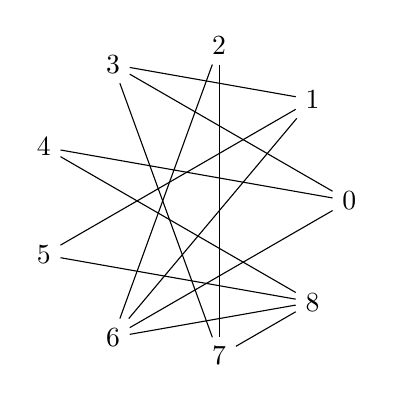
\begin{tikzpicture}
      \draw
        (0.0:2) node (0){0}
        (40.0:2) node (1){1}
        (80.0:2) node (2){2}
        (120.0:2) node (3){3}
        (160.0:2) node (4){4}
        (200.0:2) node (5){5}
        (240.0:2) node (6){6}
        (280.0:2) node (7){7}
        (320.0:2) node (8){8};
      \begin{scope}[-]
        \draw (0) to (3);
        \draw (0) to (4);
        \draw (0) to (6);
        \draw (1) to (3);
        \draw (1) to (5);
        \draw (1) to (6);
        \draw (2) to (6);
        \draw (2) to (7);
        \draw (3) to (7);
        \draw (4) to (8);
        \draw (5) to (8);
        \draw (6) to (8);
        \draw (7) to (8);
      \end{scope}
    \end{tikzpicture}
\end{figure}
\begin{itemize}
\item signature: 001101000101100000110000100001001011
\item g: Graph with 9 nodes and 13 edges
\item order: 9
\item size: 13
\item max degree: 4
\item degrees: 2,2,2,3,3,3,3,4,4
\item is tree: 0
\item is bipartite: 0
\item has bridge: 0
\item is chordal: 0
\item is complete: 0
\item min cycle basis weight: 21
\item min cycle basis size: 5
\item diameter: 3
\item radius: 2
\item is eulerian: 0
\item is planar: 0
\item number of faces: 6
\item is regular: 0
\item p3: 27
\item p4: 38
\item property hash: c61b606fe101446420ebfe3c2c86e05eae35c9b0a26446fb6b42f8f6d8fa0bff
\end{itemize}
\newpage
\begin{figure}
  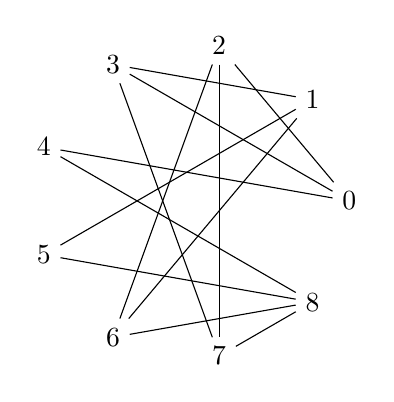
\begin{tikzpicture}
      \draw
        (0.0:2) node (0){0}
        (40.0:2) node (1){1}
        (80.0:2) node (2){2}
        (120.0:2) node (3){3}
        (160.0:2) node (4){4}
        (200.0:2) node (5){5}
        (240.0:2) node (6){6}
        (280.0:2) node (7){7}
        (320.0:2) node (8){8};
      \begin{scope}[-]
        \draw (0) to (2);
        \draw (0) to (3);
        \draw (0) to (4);
        \draw (1) to (3);
        \draw (1) to (5);
        \draw (1) to (6);
        \draw (2) to (6);
        \draw (2) to (7);
        \draw (3) to (7);
        \draw (4) to (8);
        \draw (5) to (8);
        \draw (6) to (8);
        \draw (7) to (8);
      \end{scope}
    \end{tikzpicture}
\end{figure}
\begin{itemize}
\item signature: 011100000101100000110000100001001011
\item g: Graph with 9 nodes and 13 edges
\item order: 9
\item size: 13
\item max degree: 4
\item degrees: 2,2,3,3,3,3,3,3,4
\item is tree: 0
\item is bipartite: 0
\item has bridge: 0
\item is chordal: 0
\item is complete: 0
\item min cycle basis weight: 22
\item min cycle basis size: 5
\item diameter: 3
\item radius: 2
\item is eulerian: 0
\item is planar: 0
\item number of faces: 6
\item is regular: 0
\item p3: 26
\item p4: 38
\item property hash: b0ab4585cd08b45834245812951546a171acdfd90ec8ce7e188be9f9a98ed7e8
\end{itemize}
\newpage
\begin{figure}
  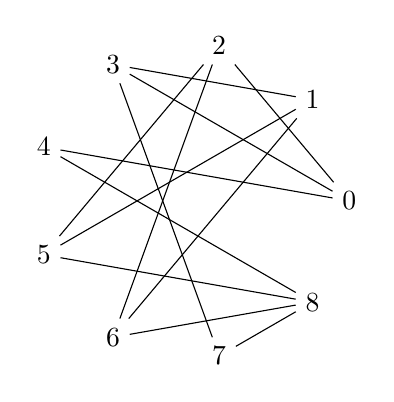
\begin{tikzpicture}
      \draw
        (0.0:2) node (0){0}
        (40.0:2) node (1){1}
        (80.0:2) node (2){2}
        (120.0:2) node (3){3}
        (160.0:2) node (4){4}
        (200.0:2) node (5){5}
        (240.0:2) node (6){6}
        (280.0:2) node (7){7}
        (320.0:2) node (8){8};
      \begin{scope}[-]
        \draw (0) to (2);
        \draw (0) to (3);
        \draw (0) to (4);
        \draw (1) to (3);
        \draw (1) to (5);
        \draw (1) to (6);
        \draw (2) to (5);
        \draw (2) to (6);
        \draw (3) to (7);
        \draw (4) to (8);
        \draw (5) to (8);
        \draw (6) to (8);
        \draw (7) to (8);
      \end{scope}
    \end{tikzpicture}
\end{figure}
\begin{itemize}
\item signature: 011100000101100001100000100001001011
\item g: Graph with 9 nodes and 13 edges
\item order: 9
\item size: 13
\item max degree: 4
\item degrees: 2,2,3,3,3,3,3,3,4
\item is tree: 0
\item is bipartite: 0
\item has bridge: 0
\item is chordal: 0
\item is complete: 0
\item min cycle basis weight: 23
\item min cycle basis size: 5
\item diameter: 3
\item radius: 2
\item is eulerian: 0
\item is planar: 0
\item number of faces: 6
\item is regular: 0
\item p3: 26
\item p4: 38
\item property hash: 229ecfa802bf007eb70ffe8b0f6bd86508514b291fcdadc4aa9e10aeba1522dd
\end{itemize}
\newpage
\begin{figure}
  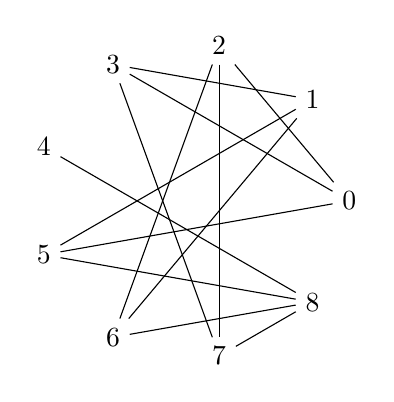
\begin{tikzpicture}
      \draw
        (0.0:2) node (0){0}
        (40.0:2) node (1){1}
        (80.0:2) node (2){2}
        (120.0:2) node (3){3}
        (160.0:2) node (4){4}
        (200.0:2) node (5){5}
        (240.0:2) node (6){6}
        (280.0:2) node (7){7}
        (320.0:2) node (8){8};
      \begin{scope}[-]
        \draw (0) to (2);
        \draw (0) to (3);
        \draw (0) to (5);
        \draw (1) to (3);
        \draw (1) to (5);
        \draw (1) to (6);
        \draw (2) to (6);
        \draw (2) to (7);
        \draw (3) to (7);
        \draw (4) to (8);
        \draw (5) to (8);
        \draw (6) to (8);
        \draw (7) to (8);
      \end{scope}
    \end{tikzpicture}
\end{figure}
\begin{itemize}
\item signature: 011010000101100000110000100001001011
\item g: Graph with 9 nodes and 13 edges
\item order: 9
\item size: 13
\item max degree: 4
\item degrees: 1,3,3,3,3,3,3,3,4
\item is tree: 0
\item is bipartite: 0
\item has bridge: 1
\item is chordal: 0
\item is complete: 0
\item min cycle basis weight: 21
\item min cycle basis size: 5
\item diameter: 3
\item radius: 2
\item is eulerian: 0
\item is planar: 0
\item number of faces: 6
\item is regular: 0
\item p3: 27
\item p4: 38
\item property hash: 9dd97fc66e0706f8984929e8c1bc9e691571a273c3d967cc118bd0bf6128c8cd
\end{itemize}
\newpage
\begin{figure}
  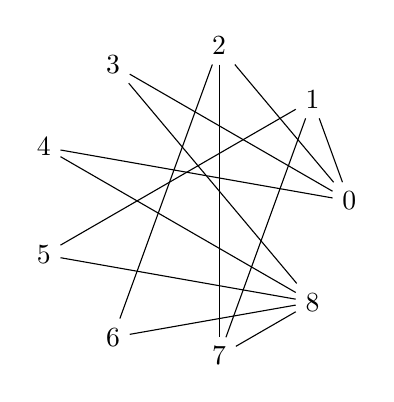
\begin{tikzpicture}
      \draw
        (0.0:2) node (0){0}
        (40.0:2) node (1){1}
        (80.0:2) node (2){2}
        (120.0:2) node (3){3}
        (160.0:2) node (4){4}
        (200.0:2) node (5){5}
        (240.0:2) node (6){6}
        (280.0:2) node (7){7}
        (320.0:2) node (8){8};
      \begin{scope}[-]
        \draw (0) to (1);
        \draw (0) to (2);
        \draw (0) to (3);
        \draw (0) to (4);
        \draw (1) to (5);
        \draw (1) to (7);
        \draw (2) to (6);
        \draw (2) to (7);
        \draw (3) to (8);
        \draw (4) to (8);
        \draw (5) to (8);
        \draw (6) to (8);
        \draw (7) to (8);
      \end{scope}
    \end{tikzpicture}
\end{figure}
\begin{itemize}
\item signature: 111100000001010000110000010001001011
\item g: Graph with 9 nodes and 13 edges
\item order: 9
\item size: 13
\item max degree: 5
\item degrees: 2,2,2,2,3,3,3,4,5
\item is tree: 0
\item is bipartite: 0
\item has bridge: 0
\item is chordal: 0
\item is complete: 0
\item min cycle basis weight: 21
\item min cycle basis size: 5
\item diameter: 3
\item radius: 2
\item is eulerian: 0
\item is planar: 1
\item number of faces: 6
\item is regular: 0
\item p3: 29
\item p4: 38
\item property hash: d09760e56c9183e185e67515b94dcf6b921ca9f20dbed017b01580c591923ac8
\end{itemize}
\newpage
\begin{figure}
  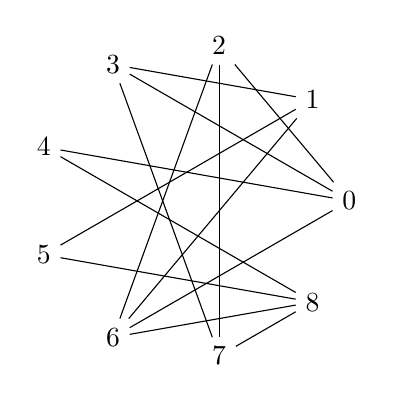
\begin{tikzpicture}
      \draw
        (0.0:2) node (0){0}
        (40.0:2) node (1){1}
        (80.0:2) node (2){2}
        (120.0:2) node (3){3}
        (160.0:2) node (4){4}
        (200.0:2) node (5){5}
        (240.0:2) node (6){6}
        (280.0:2) node (7){7}
        (320.0:2) node (8){8};
      \begin{scope}[-]
        \draw (0) to (2);
        \draw (0) to (3);
        \draw (0) to (4);
        \draw (0) to (6);
        \draw (1) to (3);
        \draw (1) to (5);
        \draw (1) to (6);
        \draw (2) to (6);
        \draw (2) to (7);
        \draw (3) to (7);
        \draw (4) to (8);
        \draw (5) to (8);
        \draw (6) to (8);
        \draw (7) to (8);
      \end{scope}
    \end{tikzpicture}
\end{figure}
\begin{itemize}
\item signature: 011101000101100000110000100001001011
\item g: Graph with 9 nodes and 14 edges
\item order: 9
\item size: 14
\item max degree: 4
\item degrees: 2,2,3,3,3,3,4,4,4
\item is tree: 0
\item is bipartite: 0
\item has bridge: 0
\item is chordal: 0
\item is complete: 0
\item min cycle basis weight: 23
\item min cycle basis size: 6
\item diameter: 3
\item radius: 2
\item is eulerian: 0
\item is planar: 0
\item number of faces: 7
\item is regular: 0
\item p3: 29
\item p4: 38
\item property hash: d2c4d7a10dba283f32035475437eb3c9881d1030559533a7869d41759890f743
\end{itemize}
\newpage
\begin{figure}
  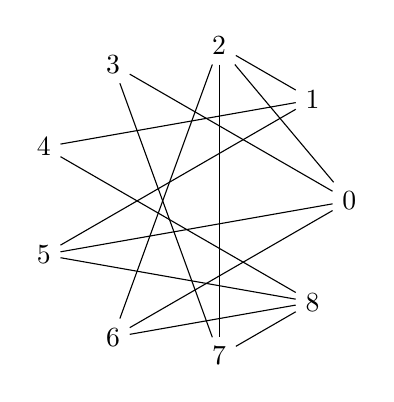
\begin{tikzpicture}
      \draw
        (0.0:2) node (0){0}
        (40.0:2) node (1){1}
        (80.0:2) node (2){2}
        (120.0:2) node (3){3}
        (160.0:2) node (4){4}
        (200.0:2) node (5){5}
        (240.0:2) node (6){6}
        (280.0:2) node (7){7}
        (320.0:2) node (8){8};
      \begin{scope}[-]
        \draw (0) to (2);
        \draw (0) to (3);
        \draw (0) to (5);
        \draw (0) to (6);
        \draw (1) to (2);
        \draw (1) to (4);
        \draw (1) to (5);
        \draw (2) to (6);
        \draw (2) to (7);
        \draw (3) to (7);
        \draw (4) to (8);
        \draw (5) to (8);
        \draw (6) to (8);
        \draw (7) to (8);
      \end{scope}
    \end{tikzpicture}
\end{figure}
\begin{itemize}
\item signature: 011011001011000000110000100001001011
\item g: Graph with 9 nodes and 14 edges
\item order: 9
\item size: 14
\item max degree: 4
\item degrees: 2,2,3,3,3,3,4,4,4
\item is tree: 0
\item is bipartite: 0
\item has bridge: 0
\item is chordal: 0
\item is complete: 0
\item min cycle basis weight: 23
\item min cycle basis size: 6
\item diameter: 3
\item radius: 2
\item is eulerian: 0
\item is planar: 0
\item number of faces: 7
\item is regular: 0
\item p3: 29
\item p4: 38
\item property hash: d2c4d7a10dba283f32035475437eb3c9881d1030559533a7869d41759890f743
\end{itemize}
\newpage
\begin{figure}
  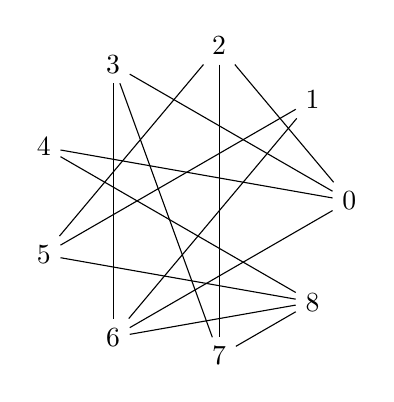
\begin{tikzpicture}
      \draw
        (0.0:2) node (0){0}
        (40.0:2) node (1){1}
        (80.0:2) node (2){2}
        (120.0:2) node (3){3}
        (160.0:2) node (4){4}
        (200.0:2) node (5){5}
        (240.0:2) node (6){6}
        (280.0:2) node (7){7}
        (320.0:2) node (8){8};
      \begin{scope}[-]
        \draw (0) to (2);
        \draw (0) to (3);
        \draw (0) to (4);
        \draw (0) to (6);
        \draw (1) to (5);
        \draw (1) to (6);
        \draw (2) to (5);
        \draw (2) to (7);
        \draw (3) to (6);
        \draw (3) to (7);
        \draw (4) to (8);
        \draw (5) to (8);
        \draw (6) to (8);
        \draw (7) to (8);
      \end{scope}
    \end{tikzpicture}
\end{figure}
\begin{itemize}
\item signature: 011101000001100001010001100001001011
\item g: Graph with 9 nodes and 14 edges
\item order: 9
\item size: 14
\item max degree: 4
\item degrees: 2,2,3,3,3,3,4,4,4
\item is tree: 0
\item is bipartite: 0
\item has bridge: 0
\item is chordal: 0
\item is complete: 0
\item min cycle basis weight: 23
\item min cycle basis size: 6
\item diameter: 3
\item radius: 2
\item is eulerian: 0
\item is planar: 0
\item number of faces: 7
\item is regular: 0
\item p3: 29
\item p4: 38
\item property hash: d2c4d7a10dba283f32035475437eb3c9881d1030559533a7869d41759890f743
\end{itemize}
\newpage
\begin{figure}
  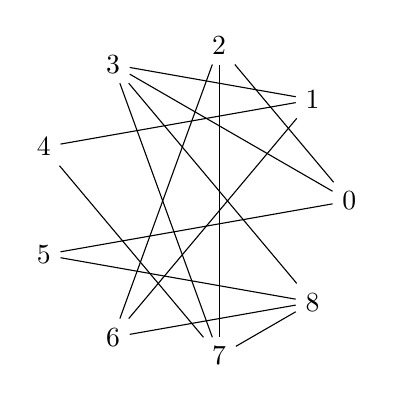
\begin{tikzpicture}
      \draw
        (0.0:2) node (0){0}
        (40.0:2) node (1){1}
        (80.0:2) node (2){2}
        (120.0:2) node (3){3}
        (160.0:2) node (4){4}
        (200.0:2) node (5){5}
        (240.0:2) node (6){6}
        (280.0:2) node (7){7}
        (320.0:2) node (8){8};
      \begin{scope}[-]
        \draw (0) to (2);
        \draw (0) to (3);
        \draw (0) to (5);
        \draw (1) to (3);
        \draw (1) to (4);
        \draw (1) to (6);
        \draw (2) to (6);
        \draw (2) to (7);
        \draw (3) to (7);
        \draw (3) to (8);
        \draw (4) to (7);
        \draw (5) to (8);
        \draw (6) to (8);
        \draw (7) to (8);
      \end{scope}
    \end{tikzpicture}
\end{figure}
\begin{itemize}
\item signature: 011010000110100000110000110010001011
\item g: Graph with 9 nodes and 14 edges
\item order: 9
\item size: 14
\item max degree: 4
\item degrees: 2,2,3,3,3,3,4,4,4
\item is tree: 0
\item is bipartite: 0
\item has bridge: 0
\item is chordal: 0
\item is complete: 0
\item min cycle basis weight: 23
\item min cycle basis size: 6
\item diameter: 3
\item radius: 2
\item is eulerian: 0
\item is planar: 0
\item number of faces: 7
\item is regular: 0
\item p3: 29
\item p4: 38
\item property hash: d2c4d7a10dba283f32035475437eb3c9881d1030559533a7869d41759890f743
\end{itemize}
\newpage
\begin{figure}
  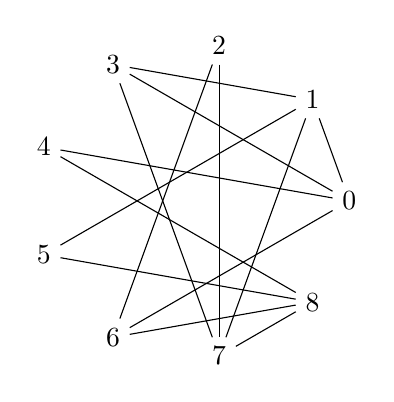
\begin{tikzpicture}
      \draw
        (0.0:2) node (0){0}
        (40.0:2) node (1){1}
        (80.0:2) node (2){2}
        (120.0:2) node (3){3}
        (160.0:2) node (4){4}
        (200.0:2) node (5){5}
        (240.0:2) node (6){6}
        (280.0:2) node (7){7}
        (320.0:2) node (8){8};
      \begin{scope}[-]
        \draw (0) to (1);
        \draw (0) to (3);
        \draw (0) to (4);
        \draw (0) to (6);
        \draw (1) to (3);
        \draw (1) to (5);
        \draw (1) to (7);
        \draw (2) to (6);
        \draw (2) to (7);
        \draw (3) to (7);
        \draw (4) to (8);
        \draw (5) to (8);
        \draw (6) to (8);
        \draw (7) to (8);
      \end{scope}
    \end{tikzpicture}
\end{figure}
\begin{itemize}
\item signature: 101101000101010000110000100001001011
\item g: Graph with 9 nodes and 14 edges
\item order: 9
\item size: 14
\item max degree: 4
\item degrees: 2,2,2,3,3,4,4,4,4
\item is tree: 0
\item is bipartite: 0
\item has bridge: 0
\item is chordal: 0
\item is complete: 0
\item min cycle basis weight: 23
\item min cycle basis size: 6
\item diameter: 3
\item radius: 2
\item is eulerian: 0
\item is planar: 1
\item number of faces: 7
\item is regular: 0
\item p3: 27
\item p4: 38
\item property hash: dfee29c3f8e7c1a634a7df5fdd6aafa54232f38793dd9d5e99ec2c7f0342bd31
\end{itemize}
\newpage
\begin{figure}
  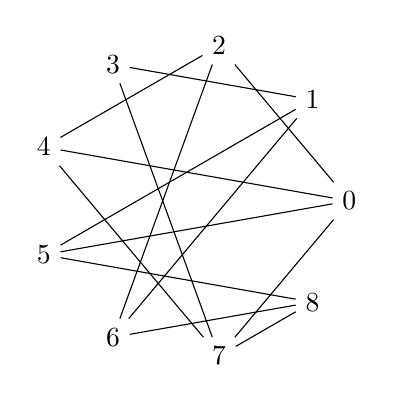
\begin{tikzpicture}
      \draw
        (0.0:2) node (0){0}
        (40.0:2) node (1){1}
        (80.0:2) node (2){2}
        (120.0:2) node (3){3}
        (160.0:2) node (4){4}
        (200.0:2) node (5){5}
        (240.0:2) node (6){6}
        (280.0:2) node (7){7}
        (320.0:2) node (8){8};
      \begin{scope}[-]
        \draw (0) to (2);
        \draw (0) to (4);
        \draw (0) to (5);
        \draw (0) to (7);
        \draw (1) to (3);
        \draw (1) to (5);
        \draw (1) to (6);
        \draw (2) to (4);
        \draw (2) to (6);
        \draw (3) to (7);
        \draw (4) to (7);
        \draw (5) to (8);
        \draw (6) to (8);
        \draw (7) to (8);
      \end{scope}
    \end{tikzpicture}
\end{figure}
\begin{itemize}
\item signature: 010110100101100010100000100010001011
\item g: Graph with 9 nodes and 14 edges
\item order: 9
\item size: 14
\item max degree: 4
\item degrees: 2,3,3,3,3,3,3,4,4
\item is tree: 0
\item is bipartite: 0
\item has bridge: 0
\item is chordal: 0
\item is complete: 0
\item min cycle basis weight: 24
\item min cycle basis size: 6
\item diameter: 3
\item radius: 2
\item is eulerian: 0
\item is planar: 0
\item number of faces: 7
\item is regular: 0
\item p3: 25
\item p4: 38
\item property hash: 6d8f0f6cfab470a0be5acb2fbc04cbdd7fa8358b0dceb04a20fa902b3298cdca
\end{itemize}
\newpage
\begin{figure}
  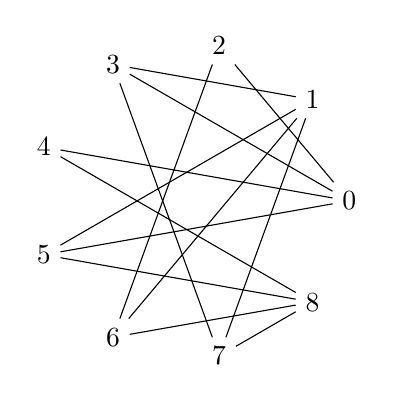
\begin{tikzpicture}
      \draw
        (0.0:2) node (0){0}
        (40.0:2) node (1){1}
        (80.0:2) node (2){2}
        (120.0:2) node (3){3}
        (160.0:2) node (4){4}
        (200.0:2) node (5){5}
        (240.0:2) node (6){6}
        (280.0:2) node (7){7}
        (320.0:2) node (8){8};
      \begin{scope}[-]
        \draw (0) to (2);
        \draw (0) to (3);
        \draw (0) to (4);
        \draw (0) to (5);
        \draw (1) to (3);
        \draw (1) to (5);
        \draw (1) to (6);
        \draw (1) to (7);
        \draw (2) to (6);
        \draw (3) to (7);
        \draw (4) to (8);
        \draw (5) to (8);
        \draw (6) to (8);
        \draw (7) to (8);
      \end{scope}
    \end{tikzpicture}
\end{figure}
\begin{itemize}
\item signature: 011110000101110000100000100001001011
\item g: Graph with 9 nodes and 14 edges
\item order: 9
\item size: 14
\item max degree: 4
\item degrees: 2,2,3,3,3,3,4,4,4
\item is tree: 0
\item is bipartite: 0
\item has bridge: 0
\item is chordal: 0
\item is complete: 0
\item min cycle basis weight: 24
\item min cycle basis size: 6
\item diameter: 3
\item radius: 2
\item is eulerian: 0
\item is planar: 0
\item number of faces: 7
\item is regular: 0
\item p3: 29
\item p4: 38
\item property hash: 1e73fe063a76a3b2c1a4bfba91b5c43ca7f0f9791c67f2c298b41464b5d42c96
\end{itemize}
\newpage
\begin{figure}
  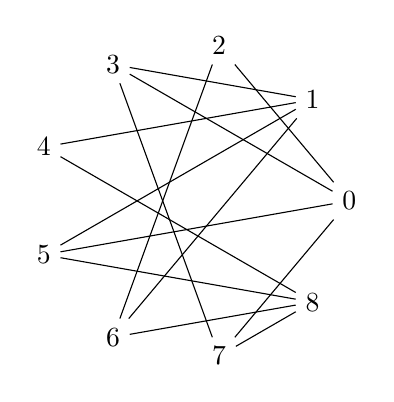
\begin{tikzpicture}
      \draw
        (0.0:2) node (0){0}
        (40.0:2) node (1){1}
        (80.0:2) node (2){2}
        (120.0:2) node (3){3}
        (160.0:2) node (4){4}
        (200.0:2) node (5){5}
        (240.0:2) node (6){6}
        (280.0:2) node (7){7}
        (320.0:2) node (8){8};
      \begin{scope}[-]
        \draw (0) to (2);
        \draw (0) to (3);
        \draw (0) to (5);
        \draw (0) to (7);
        \draw (1) to (3);
        \draw (1) to (4);
        \draw (1) to (5);
        \draw (1) to (6);
        \draw (2) to (6);
        \draw (3) to (7);
        \draw (4) to (8);
        \draw (5) to (8);
        \draw (6) to (8);
        \draw (7) to (8);
      \end{scope}
    \end{tikzpicture}
\end{figure}
\begin{itemize}
\item signature: 011010100111100000100000100001001011
\item g: Graph with 9 nodes and 14 edges
\item order: 9
\item size: 14
\item max degree: 4
\item degrees: 2,2,3,3,3,3,4,4,4
\item is tree: 0
\item is bipartite: 0
\item has bridge: 0
\item is chordal: 0
\item is complete: 0
\item min cycle basis weight: 24
\item min cycle basis size: 6
\item diameter: 3
\item radius: 2
\item is eulerian: 0
\item is planar: 0
\item number of faces: 7
\item is regular: 0
\item p3: 29
\item p4: 38
\item property hash: 1e73fe063a76a3b2c1a4bfba91b5c43ca7f0f9791c67f2c298b41464b5d42c96
\end{itemize}
\newpage
\begin{figure}
  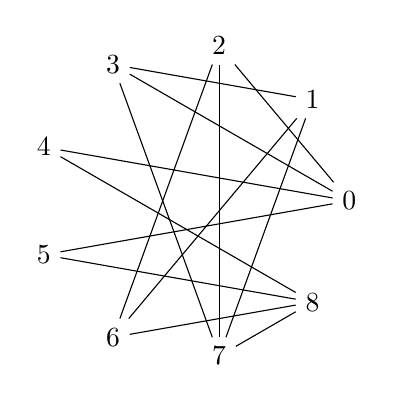
\begin{tikzpicture}
      \draw
        (0.0:2) node (0){0}
        (40.0:2) node (1){1}
        (80.0:2) node (2){2}
        (120.0:2) node (3){3}
        (160.0:2) node (4){4}
        (200.0:2) node (5){5}
        (240.0:2) node (6){6}
        (280.0:2) node (7){7}
        (320.0:2) node (8){8};
      \begin{scope}[-]
        \draw (0) to (2);
        \draw (0) to (3);
        \draw (0) to (4);
        \draw (0) to (5);
        \draw (1) to (3);
        \draw (1) to (6);
        \draw (1) to (7);
        \draw (2) to (6);
        \draw (2) to (7);
        \draw (3) to (7);
        \draw (4) to (8);
        \draw (5) to (8);
        \draw (6) to (8);
        \draw (7) to (8);
      \end{scope}
    \end{tikzpicture}
\end{figure}
\begin{itemize}
\item signature: 011110000100110000110000100001001011
\item g: Graph with 9 nodes and 14 edges
\item order: 9
\item size: 14
\item max degree: 4
\item degrees: 2,2,3,3,3,3,4,4,4
\item is tree: 0
\item is bipartite: 0
\item has bridge: 0
\item is chordal: 0
\item is complete: 0
\item min cycle basis weight: 24
\item min cycle basis size: 6
\item diameter: 3
\item radius: 2
\item is eulerian: 0
\item is planar: 0
\item number of faces: 7
\item is regular: 0
\item p3: 29
\item p4: 38
\item property hash: 1e73fe063a76a3b2c1a4bfba91b5c43ca7f0f9791c67f2c298b41464b5d42c96
\end{itemize}
\newpage
\begin{figure}
  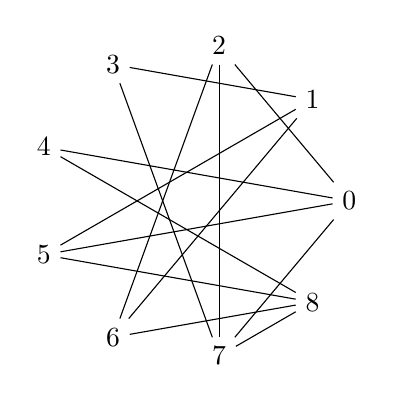
\begin{tikzpicture}
      \draw
        (0.0:2) node (0){0}
        (40.0:2) node (1){1}
        (80.0:2) node (2){2}
        (120.0:2) node (3){3}
        (160.0:2) node (4){4}
        (200.0:2) node (5){5}
        (240.0:2) node (6){6}
        (280.0:2) node (7){7}
        (320.0:2) node (8){8};
      \begin{scope}[-]
        \draw (0) to (2);
        \draw (0) to (4);
        \draw (0) to (5);
        \draw (0) to (7);
        \draw (1) to (3);
        \draw (1) to (5);
        \draw (1) to (6);
        \draw (2) to (6);
        \draw (2) to (7);
        \draw (3) to (7);
        \draw (4) to (8);
        \draw (5) to (8);
        \draw (6) to (8);
        \draw (7) to (8);
      \end{scope}
    \end{tikzpicture}
\end{figure}
\begin{itemize}
\item signature: 010110100101100000110000100001001011
\item g: Graph with 9 nodes and 14 edges
\item order: 9
\item size: 14
\item max degree: 4
\item degrees: 2,2,3,3,3,3,4,4,4
\item is tree: 0
\item is bipartite: 0
\item has bridge: 0
\item is chordal: 0
\item is complete: 0
\item min cycle basis weight: 24
\item min cycle basis size: 6
\item diameter: 3
\item radius: 2
\item is eulerian: 0
\item is planar: 0
\item number of faces: 7
\item is regular: 0
\item p3: 29
\item p4: 38
\item property hash: 1e73fe063a76a3b2c1a4bfba91b5c43ca7f0f9791c67f2c298b41464b5d42c96
\end{itemize}
\newpage
\begin{figure}
  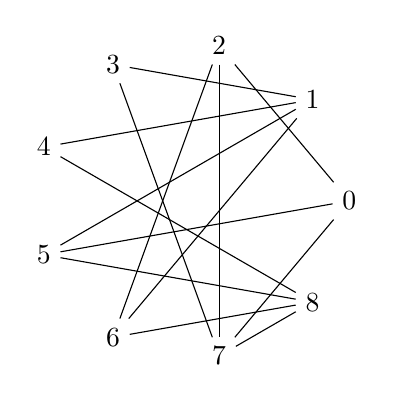
\begin{tikzpicture}
      \draw
        (0.0:2) node (0){0}
        (40.0:2) node (1){1}
        (80.0:2) node (2){2}
        (120.0:2) node (3){3}
        (160.0:2) node (4){4}
        (200.0:2) node (5){5}
        (240.0:2) node (6){6}
        (280.0:2) node (7){7}
        (320.0:2) node (8){8};
      \begin{scope}[-]
        \draw (0) to (2);
        \draw (0) to (5);
        \draw (0) to (7);
        \draw (1) to (3);
        \draw (1) to (4);
        \draw (1) to (5);
        \draw (1) to (6);
        \draw (2) to (6);
        \draw (2) to (7);
        \draw (3) to (7);
        \draw (4) to (8);
        \draw (5) to (8);
        \draw (6) to (8);
        \draw (7) to (8);
      \end{scope}
    \end{tikzpicture}
\end{figure}
\begin{itemize}
\item signature: 010010100111100000110000100001001011
\item g: Graph with 9 nodes and 14 edges
\item order: 9
\item size: 14
\item max degree: 4
\item degrees: 2,2,3,3,3,3,4,4,4
\item is tree: 0
\item is bipartite: 0
\item has bridge: 0
\item is chordal: 0
\item is complete: 0
\item min cycle basis weight: 24
\item min cycle basis size: 6
\item diameter: 3
\item radius: 2
\item is eulerian: 0
\item is planar: 0
\item number of faces: 7
\item is regular: 0
\item p3: 29
\item p4: 38
\item property hash: 1e73fe063a76a3b2c1a4bfba91b5c43ca7f0f9791c67f2c298b41464b5d42c96
\end{itemize}
\newpage
\begin{figure}
  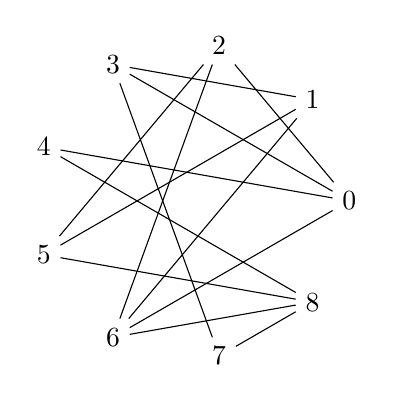
\begin{tikzpicture}
      \draw
        (0.0:2) node (0){0}
        (40.0:2) node (1){1}
        (80.0:2) node (2){2}
        (120.0:2) node (3){3}
        (160.0:2) node (4){4}
        (200.0:2) node (5){5}
        (240.0:2) node (6){6}
        (280.0:2) node (7){7}
        (320.0:2) node (8){8};
      \begin{scope}[-]
        \draw (0) to (2);
        \draw (0) to (3);
        \draw (0) to (4);
        \draw (0) to (6);
        \draw (1) to (3);
        \draw (1) to (5);
        \draw (1) to (6);
        \draw (2) to (5);
        \draw (2) to (6);
        \draw (3) to (7);
        \draw (4) to (8);
        \draw (5) to (8);
        \draw (6) to (8);
        \draw (7) to (8);
      \end{scope}
    \end{tikzpicture}
\end{figure}
\begin{itemize}
\item signature: 011101000101100001100000100001001011
\item g: Graph with 9 nodes and 14 edges
\item order: 9
\item size: 14
\item max degree: 4
\item degrees: 2,2,3,3,3,3,4,4,4
\item is tree: 0
\item is bipartite: 0
\item has bridge: 0
\item is chordal: 0
\item is complete: 0
\item min cycle basis weight: 24
\item min cycle basis size: 6
\item diameter: 3
\item radius: 2
\item is eulerian: 0
\item is planar: 0
\item number of faces: 7
\item is regular: 0
\item p3: 29
\item p4: 38
\item property hash: 1e73fe063a76a3b2c1a4bfba91b5c43ca7f0f9791c67f2c298b41464b5d42c96
\end{itemize}
\newpage
\begin{figure}
  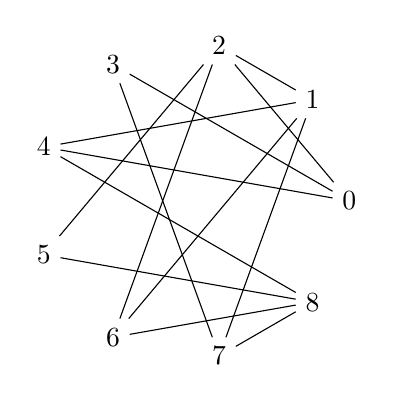
\begin{tikzpicture}
      \draw
        (0.0:2) node (0){0}
        (40.0:2) node (1){1}
        (80.0:2) node (2){2}
        (120.0:2) node (3){3}
        (160.0:2) node (4){4}
        (200.0:2) node (5){5}
        (240.0:2) node (6){6}
        (280.0:2) node (7){7}
        (320.0:2) node (8){8};
      \begin{scope}[-]
        \draw (0) to (2);
        \draw (0) to (3);
        \draw (0) to (4);
        \draw (1) to (2);
        \draw (1) to (4);
        \draw (1) to (6);
        \draw (1) to (7);
        \draw (2) to (5);
        \draw (2) to (6);
        \draw (3) to (7);
        \draw (4) to (8);
        \draw (5) to (8);
        \draw (6) to (8);
        \draw (7) to (8);
      \end{scope}
    \end{tikzpicture}
\end{figure}
\begin{itemize}
\item signature: 011100001010110001100000100001001011
\item g: Graph with 9 nodes and 14 edges
\item order: 9
\item size: 14
\item max degree: 4
\item degrees: 2,2,3,3,3,3,4,4,4
\item is tree: 0
\item is bipartite: 0
\item has bridge: 0
\item is chordal: 0
\item is complete: 0
\item min cycle basis weight: 24
\item min cycle basis size: 6
\item diameter: 3
\item radius: 2
\item is eulerian: 0
\item is planar: 0
\item number of faces: 7
\item is regular: 0
\item p3: 29
\item p4: 38
\item property hash: 1e73fe063a76a3b2c1a4bfba91b5c43ca7f0f9791c67f2c298b41464b5d42c96
\end{itemize}
\newpage
\begin{figure}
  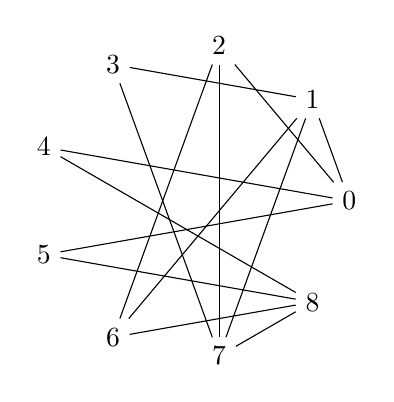
\begin{tikzpicture}
      \draw
        (0.0:2) node (0){0}
        (40.0:2) node (1){1}
        (80.0:2) node (2){2}
        (120.0:2) node (3){3}
        (160.0:2) node (4){4}
        (200.0:2) node (5){5}
        (240.0:2) node (6){6}
        (280.0:2) node (7){7}
        (320.0:2) node (8){8};
      \begin{scope}[-]
        \draw (0) to (1);
        \draw (0) to (2);
        \draw (0) to (4);
        \draw (0) to (5);
        \draw (1) to (3);
        \draw (1) to (6);
        \draw (1) to (7);
        \draw (2) to (6);
        \draw (2) to (7);
        \draw (3) to (7);
        \draw (4) to (8);
        \draw (5) to (8);
        \draw (6) to (8);
        \draw (7) to (8);
      \end{scope}
    \end{tikzpicture}
\end{figure}
\begin{itemize}
\item signature: 110110000100110000110000100001001011
\item g: Graph with 9 nodes and 14 edges
\item order: 9
\item size: 14
\item max degree: 4
\item degrees: 2,2,2,3,3,4,4,4,4
\item is tree: 0
\item is bipartite: 0
\item has bridge: 0
\item is chordal: 0
\item is complete: 0
\item min cycle basis weight: 24
\item min cycle basis size: 6
\item diameter: 3
\item radius: 2
\item is eulerian: 0
\item is planar: 0
\item number of faces: 7
\item is regular: 0
\item p3: 30
\item p4: 38
\item property hash: 8e2f63d413255e50986225c539e86bc4291d75cc4e66f85ac29ece5f43e16daa
\end{itemize}
\newpage
\begin{figure}
  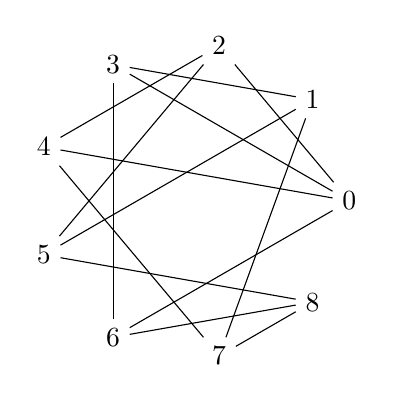
\begin{tikzpicture}
      \draw
        (0.0:2) node (0){0}
        (40.0:2) node (1){1}
        (80.0:2) node (2){2}
        (120.0:2) node (3){3}
        (160.0:2) node (4){4}
        (200.0:2) node (5){5}
        (240.0:2) node (6){6}
        (280.0:2) node (7){7}
        (320.0:2) node (8){8};
      \begin{scope}[-]
        \draw (0) to (2);
        \draw (0) to (3);
        \draw (0) to (4);
        \draw (0) to (6);
        \draw (1) to (3);
        \draw (1) to (5);
        \draw (1) to (7);
        \draw (2) to (4);
        \draw (2) to (5);
        \draw (3) to (6);
        \draw (4) to (7);
        \draw (5) to (8);
        \draw (6) to (8);
        \draw (7) to (8);
      \end{scope}
    \end{tikzpicture}
\end{figure}
\begin{itemize}
\item signature: 011101000101010011000001000010001011
\item g: Graph with 9 nodes and 14 edges
\item order: 9
\item size: 14
\item max degree: 4
\item degrees: 3,3,3,3,3,3,3,3,4
\item is tree: 0
\item is bipartite: 0
\item has bridge: 0
\item is chordal: 0
\item is complete: 0
\item min cycle basis weight: 25
\item min cycle basis size: 6
\item diameter: 2
\item radius: 2
\item is eulerian: 0
\item is planar: 0
\item number of faces: 7
\item is regular: 0
\item p3: 24
\item p4: 38
\item property hash: 406c413572f61640edf72c6b3d9c0624affd5f593370e23c7a89b87a17e2e680
\end{itemize}
\newpage
\begin{figure}
  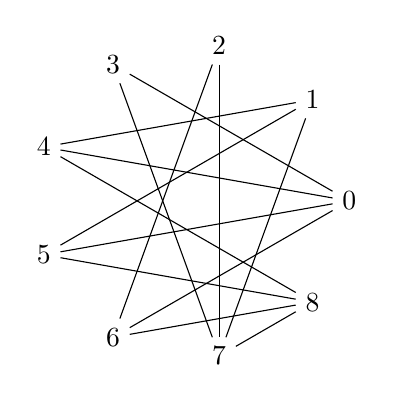
\begin{tikzpicture}
      \draw
        (0.0:2) node (0){0}
        (40.0:2) node (1){1}
        (80.0:2) node (2){2}
        (120.0:2) node (3){3}
        (160.0:2) node (4){4}
        (200.0:2) node (5){5}
        (240.0:2) node (6){6}
        (280.0:2) node (7){7}
        (320.0:2) node (8){8};
      \begin{scope}[-]
        \draw (0) to (3);
        \draw (0) to (4);
        \draw (0) to (5);
        \draw (0) to (6);
        \draw (1) to (4);
        \draw (1) to (5);
        \draw (1) to (7);
        \draw (2) to (6);
        \draw (2) to (7);
        \draw (3) to (7);
        \draw (4) to (8);
        \draw (5) to (8);
        \draw (6) to (8);
        \draw (7) to (8);
      \end{scope}
    \end{tikzpicture}
\end{figure}
\begin{itemize}
\item signature: 001111000011010000110000100001001011
\item g: Graph with 9 nodes and 14 edges
\item order: 9
\item size: 14
\item max degree: 4
\item degrees: 2,2,3,3,3,3,4,4,4
\item is tree: 0
\item is bipartite: 0
\item has bridge: 0
\item is chordal: 0
\item is complete: 0
\item min cycle basis weight: 25
\item min cycle basis size: 6
\item diameter: 3
\item radius: 2
\item is eulerian: 0
\item is planar: 0
\item number of faces: 7
\item is regular: 0
\item p3: 32
\item p4: 38
\item property hash: 96676ca1d896b13295aea7d66a2a89421b6edd99985c3d8a83f91889353cf116
\end{itemize}
\newpage
\begin{figure}
  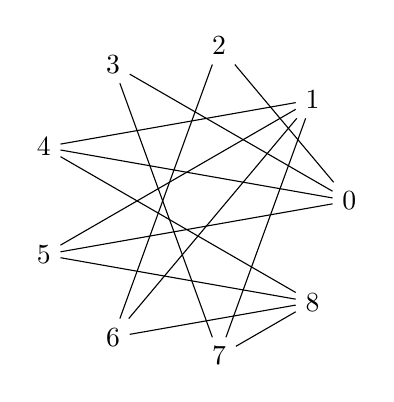
\begin{tikzpicture}
      \draw
        (0.0:2) node (0){0}
        (40.0:2) node (1){1}
        (80.0:2) node (2){2}
        (120.0:2) node (3){3}
        (160.0:2) node (4){4}
        (200.0:2) node (5){5}
        (240.0:2) node (6){6}
        (280.0:2) node (7){7}
        (320.0:2) node (8){8};
      \begin{scope}[-]
        \draw (0) to (2);
        \draw (0) to (3);
        \draw (0) to (4);
        \draw (0) to (5);
        \draw (1) to (4);
        \draw (1) to (5);
        \draw (1) to (6);
        \draw (1) to (7);
        \draw (2) to (6);
        \draw (3) to (7);
        \draw (4) to (8);
        \draw (5) to (8);
        \draw (6) to (8);
        \draw (7) to (8);
      \end{scope}
    \end{tikzpicture}
\end{figure}
\begin{itemize}
\item signature: 011110000011110000100000100001001011
\item g: Graph with 9 nodes and 14 edges
\item order: 9
\item size: 14
\item max degree: 4
\item degrees: 2,2,3,3,3,3,4,4,4
\item is tree: 0
\item is bipartite: 0
\item has bridge: 0
\item is chordal: 0
\item is complete: 0
\item min cycle basis weight: 26
\item min cycle basis size: 6
\item diameter: 3
\item radius: 2
\item is eulerian: 0
\item is planar: 0
\item number of faces: 7
\item is regular: 0
\item p3: 32
\item p4: 38
\item property hash: 0639c540c86ff654d0b3d1b4ba4ba029d5cb7744f5c77340400057dbf447a5b5
\end{itemize}
\newpage
\begin{figure}
  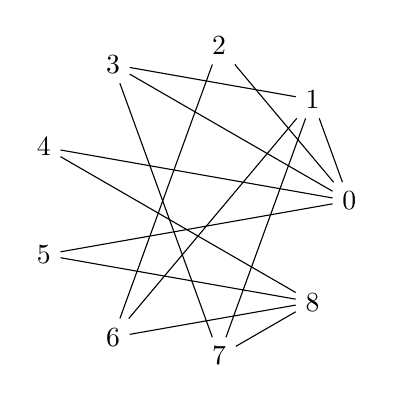
\begin{tikzpicture}
      \draw
        (0.0:2) node (0){0}
        (40.0:2) node (1){1}
        (80.0:2) node (2){2}
        (120.0:2) node (3){3}
        (160.0:2) node (4){4}
        (200.0:2) node (5){5}
        (240.0:2) node (6){6}
        (280.0:2) node (7){7}
        (320.0:2) node (8){8};
      \begin{scope}[-]
        \draw (0) to (1);
        \draw (0) to (2);
        \draw (0) to (3);
        \draw (0) to (4);
        \draw (0) to (5);
        \draw (1) to (3);
        \draw (1) to (6);
        \draw (1) to (7);
        \draw (2) to (6);
        \draw (3) to (7);
        \draw (4) to (8);
        \draw (5) to (8);
        \draw (6) to (8);
        \draw (7) to (8);
      \end{scope}
    \end{tikzpicture}
\end{figure}
\begin{itemize}
\item signature: 111110000100110000100000100001001011
\item g: Graph with 9 nodes and 14 edges
\item order: 9
\item size: 14
\item max degree: 5
\item degrees: 2,2,2,3,3,3,4,4,5
\item is tree: 0
\item is bipartite: 0
\item has bridge: 0
\item is chordal: 0
\item is complete: 0
\item min cycle basis weight: 23
\item min cycle basis size: 6
\item diameter: 3
\item radius: 2
\item is eulerian: 0
\item is planar: 1
\item number of faces: 7
\item is regular: 0
\item p3: 28
\item p4: 38
\item property hash: 55fcfe61ab4f159e5a7b9fd28cc53d802cc6c33580b5c613872f4a920d47db7d
\end{itemize}
\newpage
\begin{figure}
  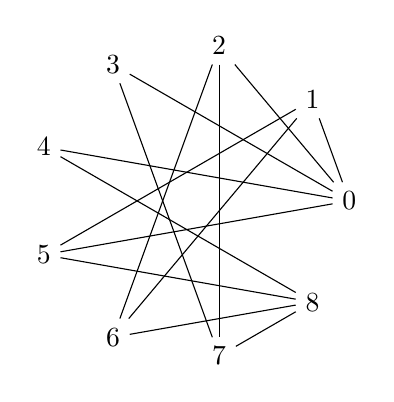
\begin{tikzpicture}
      \draw
        (0.0:2) node (0){0}
        (40.0:2) node (1){1}
        (80.0:2) node (2){2}
        (120.0:2) node (3){3}
        (160.0:2) node (4){4}
        (200.0:2) node (5){5}
        (240.0:2) node (6){6}
        (280.0:2) node (7){7}
        (320.0:2) node (8){8};
      \begin{scope}[-]
        \draw (0) to (1);
        \draw (0) to (2);
        \draw (0) to (3);
        \draw (0) to (4);
        \draw (0) to (5);
        \draw (1) to (5);
        \draw (1) to (6);
        \draw (2) to (6);
        \draw (2) to (7);
        \draw (3) to (7);
        \draw (4) to (8);
        \draw (5) to (8);
        \draw (6) to (8);
        \draw (7) to (8);
      \end{scope}
    \end{tikzpicture}
\end{figure}
\begin{itemize}
\item signature: 111110000001100000110000100001001011
\item g: Graph with 9 nodes and 14 edges
\item order: 9
\item size: 14
\item max degree: 5
\item degrees: 2,2,3,3,3,3,3,4,5
\item is tree: 0
\item is bipartite: 0
\item has bridge: 0
\item is chordal: 0
\item is complete: 0
\item min cycle basis weight: 23
\item min cycle basis size: 6
\item diameter: 3
\item radius: 2
\item is eulerian: 0
\item is planar: 1
\item number of faces: 7
\item is regular: 0
\item p3: 30
\item p4: 38
\item property hash: 9e161aa9aafd1a437273c0fe074486ef831ccc1b64923092e65bdc084dc8be2e
\end{itemize}
\newpage
\begin{figure}
  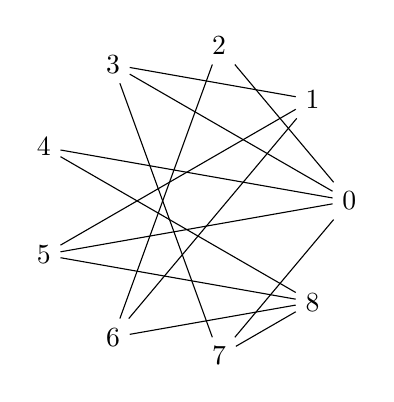
\begin{tikzpicture}
      \draw
        (0.0:2) node (0){0}
        (40.0:2) node (1){1}
        (80.0:2) node (2){2}
        (120.0:2) node (3){3}
        (160.0:2) node (4){4}
        (200.0:2) node (5){5}
        (240.0:2) node (6){6}
        (280.0:2) node (7){7}
        (320.0:2) node (8){8};
      \begin{scope}[-]
        \draw (0) to (2);
        \draw (0) to (3);
        \draw (0) to (4);
        \draw (0) to (5);
        \draw (0) to (7);
        \draw (1) to (3);
        \draw (1) to (5);
        \draw (1) to (6);
        \draw (2) to (6);
        \draw (3) to (7);
        \draw (4) to (8);
        \draw (5) to (8);
        \draw (6) to (8);
        \draw (7) to (8);
      \end{scope}
    \end{tikzpicture}
\end{figure}
\begin{itemize}
\item signature: 011110100101100000100000100001001011
\item g: Graph with 9 nodes and 14 edges
\item order: 9
\item size: 14
\item max degree: 5
\item degrees: 2,2,3,3,3,3,3,4,5
\item is tree: 0
\item is bipartite: 0
\item has bridge: 0
\item is chordal: 0
\item is complete: 0
\item min cycle basis weight: 24
\item min cycle basis size: 6
\item diameter: 3
\item radius: 2
\item is eulerian: 0
\item is planar: 0
\item number of faces: 7
\item is regular: 0
\item p3: 30
\item p4: 38
\item property hash: 789c5b494b46e9823caca4cde5a1d481b194960d898e99deab8a4bbb11fd2a30
\end{itemize}
\newpage
\begin{figure}
  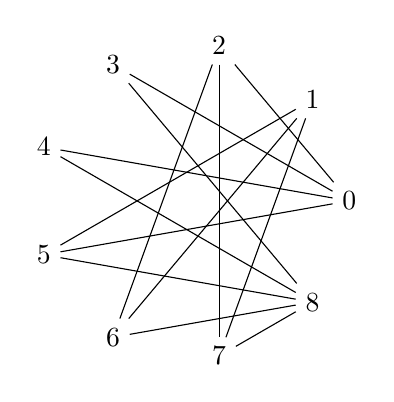
\begin{tikzpicture}
      \draw
        (0.0:2) node (0){0}
        (40.0:2) node (1){1}
        (80.0:2) node (2){2}
        (120.0:2) node (3){3}
        (160.0:2) node (4){4}
        (200.0:2) node (5){5}
        (240.0:2) node (6){6}
        (280.0:2) node (7){7}
        (320.0:2) node (8){8};
      \begin{scope}[-]
        \draw (0) to (2);
        \draw (0) to (3);
        \draw (0) to (4);
        \draw (0) to (5);
        \draw (1) to (5);
        \draw (1) to (6);
        \draw (1) to (7);
        \draw (2) to (6);
        \draw (2) to (7);
        \draw (3) to (8);
        \draw (4) to (8);
        \draw (5) to (8);
        \draw (6) to (8);
        \draw (7) to (8);
      \end{scope}
    \end{tikzpicture}
\end{figure}
\begin{itemize}
\item signature: 011110000001110000110000010001001011
\item g: Graph with 9 nodes and 14 edges
\item order: 9
\item size: 14
\item max degree: 5
\item degrees: 2,2,3,3,3,3,3,4,5
\item is tree: 0
\item is bipartite: 0
\item has bridge: 0
\item is chordal: 0
\item is complete: 0
\item min cycle basis weight: 25
\item min cycle basis size: 6
\item diameter: 3
\item radius: 2
\item is eulerian: 0
\item is planar: 0
\item number of faces: 7
\item is regular: 0
\item p3: 33
\item p4: 38
\item property hash: 51e558222fa54e9875e824650105f94cd545ffb33d07c5ef3b171ba34b57af58
\end{itemize}
\newpage
\begin{figure}
  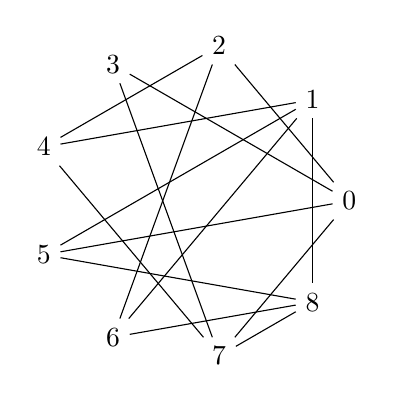
\begin{tikzpicture}
      \draw
        (0.0:2) node (0){0}
        (40.0:2) node (1){1}
        (80.0:2) node (2){2}
        (120.0:2) node (3){3}
        (160.0:2) node (4){4}
        (200.0:2) node (5){5}
        (240.0:2) node (6){6}
        (280.0:2) node (7){7}
        (320.0:2) node (8){8};
      \begin{scope}[-]
        \draw (0) to (2);
        \draw (0) to (3);
        \draw (0) to (5);
        \draw (0) to (7);
        \draw (1) to (4);
        \draw (1) to (5);
        \draw (1) to (6);
        \draw (1) to (8);
        \draw (2) to (4);
        \draw (2) to (6);
        \draw (3) to (7);
        \draw (4) to (7);
        \draw (5) to (8);
        \draw (6) to (8);
        \draw (7) to (8);
      \end{scope}
    \end{tikzpicture}
\end{figure}
\begin{itemize}
\item signature: 011010100011101010100000100010001011
\item g: Graph with 9 nodes and 15 edges
\item order: 9
\item size: 15
\item max degree: 4
\item degrees: 2,3,3,3,3,4,4,4,4
\item is tree: 0
\item is bipartite: 0
\item has bridge: 0
\item is chordal: 0
\item is complete: 0
\item min cycle basis weight: 25
\item min cycle basis size: 7
\item diameter: 3
\item radius: 2
\item is eulerian: 0
\item is planar: 0
\item number of faces: 8
\item is regular: 0
\item p3: 28
\item p4: 38
\item property hash: dadfbdacd8fc172611c69179dfd85a8244b9b873f8830df66b47c73156d3746c
\end{itemize}
\newpage
\begin{figure}
  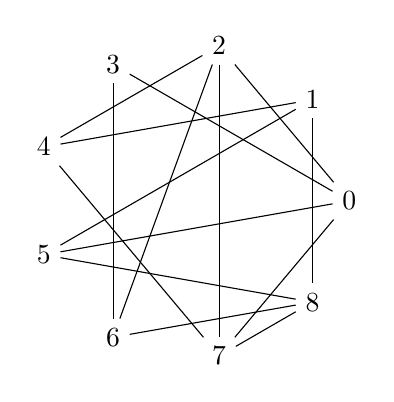
\begin{tikzpicture}
      \draw
        (0.0:2) node (0){0}
        (40.0:2) node (1){1}
        (80.0:2) node (2){2}
        (120.0:2) node (3){3}
        (160.0:2) node (4){4}
        (200.0:2) node (5){5}
        (240.0:2) node (6){6}
        (280.0:2) node (7){7}
        (320.0:2) node (8){8};
      \begin{scope}[-]
        \draw (0) to (2);
        \draw (0) to (3);
        \draw (0) to (5);
        \draw (0) to (7);
        \draw (1) to (4);
        \draw (1) to (5);
        \draw (1) to (8);
        \draw (2) to (4);
        \draw (2) to (6);
        \draw (2) to (7);
        \draw (3) to (6);
        \draw (4) to (7);
        \draw (5) to (8);
        \draw (6) to (8);
        \draw (7) to (8);
      \end{scope}
    \end{tikzpicture}
\end{figure}
\begin{itemize}
\item signature: 011010100011001010110001000010001011
\item g: Graph with 9 nodes and 15 edges
\item order: 9
\item size: 15
\item max degree: 4
\item degrees: 2,3,3,3,3,4,4,4,4
\item is tree: 0
\item is bipartite: 0
\item has bridge: 0
\item is chordal: 0
\item is complete: 0
\item min cycle basis weight: 25
\item min cycle basis size: 7
\item diameter: 3
\item radius: 2
\item is eulerian: 0
\item is planar: 0
\item number of faces: 8
\item is regular: 0
\item p3: 28
\item p4: 38
\item property hash: dadfbdacd8fc172611c69179dfd85a8244b9b873f8830df66b47c73156d3746c
\end{itemize}
\newpage
\begin{figure}
  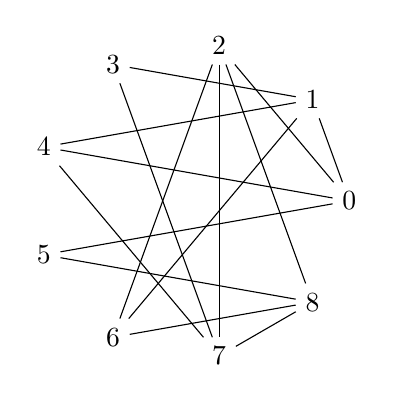
\begin{tikzpicture}
      \draw
        (0.0:2) node (0){0}
        (40.0:2) node (1){1}
        (80.0:2) node (2){2}
        (120.0:2) node (3){3}
        (160.0:2) node (4){4}
        (200.0:2) node (5){5}
        (240.0:2) node (6){6}
        (280.0:2) node (7){7}
        (320.0:2) node (8){8};
      \begin{scope}[-]
        \draw (0) to (1);
        \draw (0) to (2);
        \draw (0) to (4);
        \draw (0) to (5);
        \draw (1) to (3);
        \draw (1) to (4);
        \draw (1) to (6);
        \draw (2) to (6);
        \draw (2) to (7);
        \draw (2) to (8);
        \draw (3) to (7);
        \draw (4) to (7);
        \draw (5) to (8);
        \draw (6) to (8);
        \draw (7) to (8);
      \end{scope}
    \end{tikzpicture}
\end{figure}
\begin{itemize}
\item signature: 110110000110100000111000100010001011
\item g: Graph with 9 nodes and 15 edges
\item order: 9
\item size: 15
\item max degree: 4
\item degrees: 2,2,3,3,4,4,4,4,4
\item is tree: 0
\item is bipartite: 0
\item has bridge: 0
\item is chordal: 0
\item is complete: 0
\item min cycle basis weight: 25
\item min cycle basis size: 7
\item diameter: 3
\item radius: 2
\item is eulerian: 0
\item is planar: 0
\item number of faces: 8
\item is regular: 0
\item p3: 29
\item p4: 38
\item property hash: bd5d7669e360d6c8ca7563b0ab99968b611cf4a9810f007dbb1e4c3fd48f8851
\end{itemize}
\newpage
\begin{figure}
  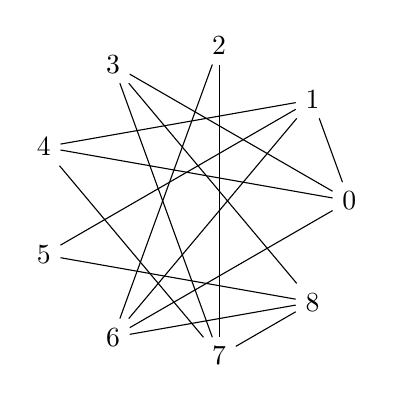
\begin{tikzpicture}
      \draw
        (0.0:2) node (0){0}
        (40.0:2) node (1){1}
        (80.0:2) node (2){2}
        (120.0:2) node (3){3}
        (160.0:2) node (4){4}
        (200.0:2) node (5){5}
        (240.0:2) node (6){6}
        (280.0:2) node (7){7}
        (320.0:2) node (8){8};
      \begin{scope}[-]
        \draw (0) to (1);
        \draw (0) to (3);
        \draw (0) to (4);
        \draw (0) to (6);
        \draw (1) to (4);
        \draw (1) to (5);
        \draw (1) to (6);
        \draw (2) to (6);
        \draw (2) to (7);
        \draw (3) to (7);
        \draw (3) to (8);
        \draw (4) to (7);
        \draw (5) to (8);
        \draw (6) to (8);
        \draw (7) to (8);
      \end{scope}
    \end{tikzpicture}
\end{figure}
\begin{itemize}
\item signature: 101101000011100000110000110010001011
\item g: Graph with 9 nodes and 15 edges
\item order: 9
\item size: 15
\item max degree: 4
\item degrees: 2,2,3,3,4,4,4,4,4
\item is tree: 0
\item is bipartite: 0
\item has bridge: 0
\item is chordal: 0
\item is complete: 0
\item min cycle basis weight: 25
\item min cycle basis size: 7
\item diameter: 3
\item radius: 2
\item is eulerian: 0
\item is planar: 0
\item number of faces: 8
\item is regular: 0
\item p3: 29
\item p4: 38
\item property hash: bd5d7669e360d6c8ca7563b0ab99968b611cf4a9810f007dbb1e4c3fd48f8851
\end{itemize}
\newpage
\begin{figure}
  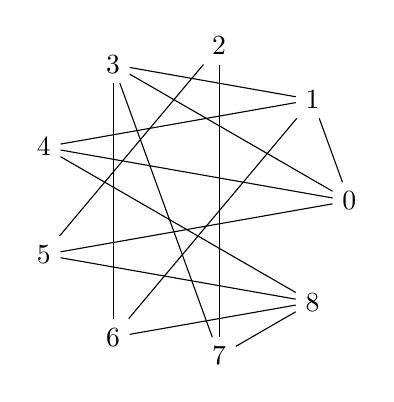
\begin{tikzpicture}
      \draw
        (0.0:2) node (0){0}
        (40.0:2) node (1){1}
        (80.0:2) node (2){2}
        (120.0:2) node (3){3}
        (160.0:2) node (4){4}
        (200.0:2) node (5){5}
        (240.0:2) node (6){6}
        (280.0:2) node (7){7}
        (320.0:2) node (8){8};
      \begin{scope}[-]
        \draw (0) to (1);
        \draw (0) to (3);
        \draw (0) to (4);
        \draw (0) to (5);
        \draw (1) to (3);
        \draw (1) to (4);
        \draw (1) to (6);
        \draw (2) to (5);
        \draw (2) to (7);
        \draw (3) to (6);
        \draw (3) to (7);
        \draw (4) to (8);
        \draw (5) to (8);
        \draw (6) to (8);
        \draw (7) to (8);
      \end{scope}
    \end{tikzpicture}
\end{figure}
\begin{itemize}
\item signature: 101110000110100001010001100001001011
\item g: Graph with 9 nodes and 15 edges
\item order: 9
\item size: 15
\item max degree: 4
\item degrees: 2,3,3,3,3,4,4,4,4
\item is tree: 0
\item is bipartite: 0
\item has bridge: 0
\item is chordal: 0
\item is complete: 0
\item min cycle basis weight: 25
\item min cycle basis size: 7
\item diameter: 3
\item radius: 2
\item is eulerian: 0
\item is planar: 1
\item number of faces: 8
\item is regular: 0
\item p3: 28
\item p4: 38
\item property hash: 2e8fb4d3ce47ffcad424ee3493a32300ddf2b0a30000d6cca5f4c1ecbfbf6ac4
\end{itemize}
\newpage
\begin{figure}
  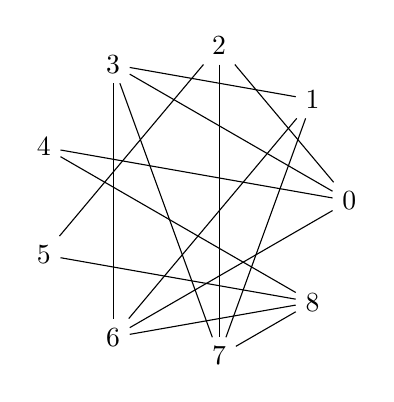
\begin{tikzpicture}
      \draw
        (0.0:2) node (0){0}
        (40.0:2) node (1){1}
        (80.0:2) node (2){2}
        (120.0:2) node (3){3}
        (160.0:2) node (4){4}
        (200.0:2) node (5){5}
        (240.0:2) node (6){6}
        (280.0:2) node (7){7}
        (320.0:2) node (8){8};
      \begin{scope}[-]
        \draw (0) to (2);
        \draw (0) to (3);
        \draw (0) to (4);
        \draw (0) to (6);
        \draw (1) to (3);
        \draw (1) to (6);
        \draw (1) to (7);
        \draw (2) to (5);
        \draw (2) to (7);
        \draw (3) to (6);
        \draw (3) to (7);
        \draw (4) to (8);
        \draw (5) to (8);
        \draw (6) to (8);
        \draw (7) to (8);
      \end{scope}
    \end{tikzpicture}
\end{figure}
\begin{itemize}
\item signature: 011101000100110001010001100001001011
\item g: Graph with 9 nodes and 15 edges
\item order: 9
\item size: 15
\item max degree: 4
\item degrees: 2,2,3,3,4,4,4,4,4
\item is tree: 0
\item is bipartite: 0
\item has bridge: 0
\item is chordal: 0
\item is complete: 0
\item min cycle basis weight: 25
\item min cycle basis size: 7
\item diameter: 3
\item radius: 2
\item is eulerian: 0
\item is planar: 1
\item number of faces: 8
\item is regular: 0
\item p3: 29
\item p4: 38
\item property hash: c89e0fd42a9fbb688918c92931e2f8b25d180c52aaf1d045ff9ed6d2624c10a8
\end{itemize}
\newpage
\begin{figure}
  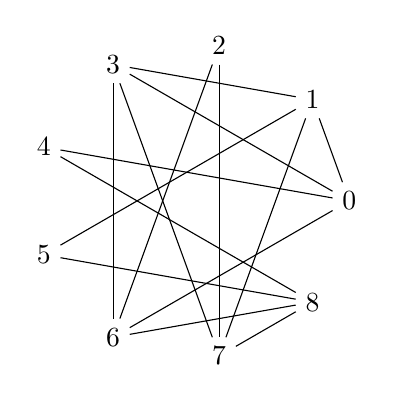
\begin{tikzpicture}
      \draw
        (0.0:2) node (0){0}
        (40.0:2) node (1){1}
        (80.0:2) node (2){2}
        (120.0:2) node (3){3}
        (160.0:2) node (4){4}
        (200.0:2) node (5){5}
        (240.0:2) node (6){6}
        (280.0:2) node (7){7}
        (320.0:2) node (8){8};
      \begin{scope}[-]
        \draw (0) to (1);
        \draw (0) to (3);
        \draw (0) to (4);
        \draw (0) to (6);
        \draw (1) to (3);
        \draw (1) to (5);
        \draw (1) to (7);
        \draw (2) to (6);
        \draw (2) to (7);
        \draw (3) to (6);
        \draw (3) to (7);
        \draw (4) to (8);
        \draw (5) to (8);
        \draw (6) to (8);
        \draw (7) to (8);
      \end{scope}
    \end{tikzpicture}
\end{figure}
\begin{itemize}
\item signature: 101101000101010000110001100001001011
\item g: Graph with 9 nodes and 15 edges
\item order: 9
\item size: 15
\item max degree: 4
\item degrees: 2,2,2,4,4,4,4,4,4
\item is tree: 0
\item is bipartite: 0
\item has bridge: 0
\item is chordal: 0
\item is complete: 0
\item min cycle basis weight: 25
\item min cycle basis size: 7
\item diameter: 3
\item radius: 2
\item is eulerian: 1
\item is planar: 1
\item number of faces: 8
\item is regular: 0
\item p3: 30
\item p4: 38
\item property hash: cf8aa3a58d4de10406b699b2b1d10fb3fddf33850786bc56a0190d087b39729f
\end{itemize}
\newpage
\begin{figure}
  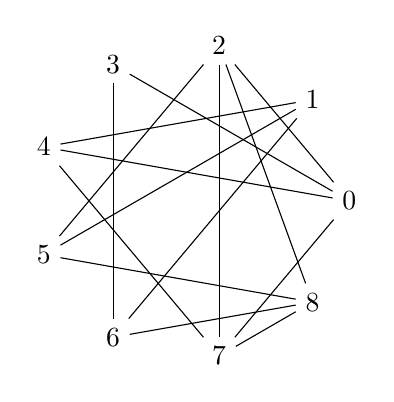
\begin{tikzpicture}
      \draw
        (0.0:2) node (0){0}
        (40.0:2) node (1){1}
        (80.0:2) node (2){2}
        (120.0:2) node (3){3}
        (160.0:2) node (4){4}
        (200.0:2) node (5){5}
        (240.0:2) node (6){6}
        (280.0:2) node (7){7}
        (320.0:2) node (8){8};
      \begin{scope}[-]
        \draw (0) to (2);
        \draw (0) to (3);
        \draw (0) to (4);
        \draw (0) to (7);
        \draw (1) to (4);
        \draw (1) to (5);
        \draw (1) to (6);
        \draw (2) to (5);
        \draw (2) to (7);
        \draw (2) to (8);
        \draw (3) to (6);
        \draw (4) to (7);
        \draw (5) to (8);
        \draw (6) to (8);
        \draw (7) to (8);
      \end{scope}
    \end{tikzpicture}
\end{figure}
\begin{itemize}
\item signature: 011100100011100001011001000010001011
\item g: Graph with 9 nodes and 15 edges
\item order: 9
\item size: 15
\item max degree: 4
\item degrees: 2,3,3,3,3,4,4,4,4
\item is tree: 0
\item is bipartite: 0
\item has bridge: 0
\item is chordal: 0
\item is complete: 0
\item min cycle basis weight: 26
\item min cycle basis size: 7
\item diameter: 3
\item radius: 2
\item is eulerian: 0
\item is planar: 0
\item number of faces: 8
\item is regular: 0
\item p3: 25
\item p4: 38
\item property hash: 80fe37187d3b923bb4b0f8534fafd79fbdf4d176272920ac0489ea59e5cacd05
\end{itemize}
\newpage
\begin{figure}
  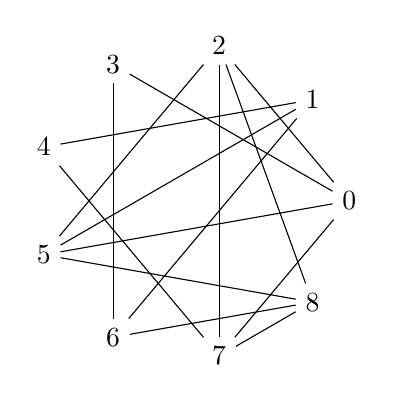
\begin{tikzpicture}
      \draw
        (0.0:2) node (0){0}
        (40.0:2) node (1){1}
        (80.0:2) node (2){2}
        (120.0:2) node (3){3}
        (160.0:2) node (4){4}
        (200.0:2) node (5){5}
        (240.0:2) node (6){6}
        (280.0:2) node (7){7}
        (320.0:2) node (8){8};
      \begin{scope}[-]
        \draw (0) to (2);
        \draw (0) to (3);
        \draw (0) to (5);
        \draw (0) to (7);
        \draw (1) to (4);
        \draw (1) to (5);
        \draw (1) to (6);
        \draw (2) to (5);
        \draw (2) to (7);
        \draw (2) to (8);
        \draw (3) to (6);
        \draw (4) to (7);
        \draw (5) to (8);
        \draw (6) to (8);
        \draw (7) to (8);
      \end{scope}
    \end{tikzpicture}
\end{figure}
\begin{itemize}
\item signature: 011010100011100001011001000010001011
\item g: Graph with 9 nodes and 15 edges
\item order: 9
\item size: 15
\item max degree: 4
\item degrees: 2,2,3,3,4,4,4,4,4
\item is tree: 0
\item is bipartite: 0
\item has bridge: 0
\item is chordal: 0
\item is complete: 0
\item min cycle basis weight: 26
\item min cycle basis size: 7
\item diameter: 3
\item radius: 2
\item is eulerian: 0
\item is planar: 0
\item number of faces: 8
\item is regular: 0
\item p3: 26
\item p4: 38
\item property hash: 0294b8663c15f806523acc7d4afdc914e724106d560f15d7588d90ce31460227
\end{itemize}
\newpage
\begin{figure}
  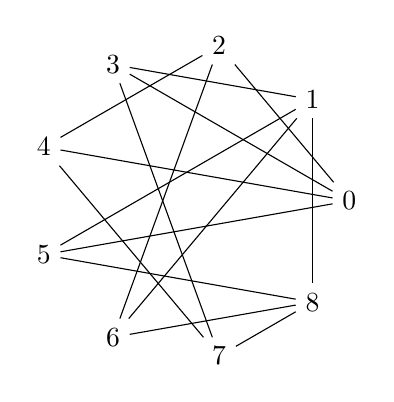
\begin{tikzpicture}
      \draw
        (0.0:2) node (0){0}
        (40.0:2) node (1){1}
        (80.0:2) node (2){2}
        (120.0:2) node (3){3}
        (160.0:2) node (4){4}
        (200.0:2) node (5){5}
        (240.0:2) node (6){6}
        (280.0:2) node (7){7}
        (320.0:2) node (8){8};
      \begin{scope}[-]
        \draw (0) to (2);
        \draw (0) to (3);
        \draw (0) to (4);
        \draw (0) to (5);
        \draw (1) to (3);
        \draw (1) to (5);
        \draw (1) to (6);
        \draw (1) to (8);
        \draw (2) to (4);
        \draw (2) to (6);
        \draw (3) to (7);
        \draw (4) to (7);
        \draw (5) to (8);
        \draw (6) to (8);
        \draw (7) to (8);
      \end{scope}
    \end{tikzpicture}
\end{figure}
\begin{itemize}
\item signature: 011110000101101010100000100010001011
\item g: Graph with 9 nodes and 15 edges
\item order: 9
\item size: 15
\item max degree: 4
\item degrees: 3,3,3,3,3,3,4,4,4
\item is tree: 0
\item is bipartite: 0
\item has bridge: 0
\item is chordal: 0
\item is complete: 0
\item min cycle basis weight: 26
\item min cycle basis size: 7
\item diameter: 3
\item radius: 2
\item is eulerian: 0
\item is planar: 0
\item number of faces: 8
\item is regular: 0
\item p3: 27
\item p4: 38
\item property hash: 5870bf19021d74c95162704bb5bd23e0eaf646bb74b2d40e7a305e46d6d0889a
\end{itemize}
\newpage
\begin{figure}
  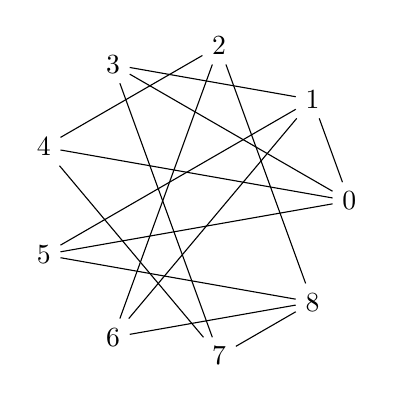
\begin{tikzpicture}
      \draw
        (0.0:2) node (0){0}
        (40.0:2) node (1){1}
        (80.0:2) node (2){2}
        (120.0:2) node (3){3}
        (160.0:2) node (4){4}
        (200.0:2) node (5){5}
        (240.0:2) node (6){6}
        (280.0:2) node (7){7}
        (320.0:2) node (8){8};
      \begin{scope}[-]
        \draw (0) to (1);
        \draw (0) to (3);
        \draw (0) to (4);
        \draw (0) to (5);
        \draw (1) to (3);
        \draw (1) to (5);
        \draw (1) to (6);
        \draw (2) to (4);
        \draw (2) to (6);
        \draw (2) to (8);
        \draw (3) to (7);
        \draw (4) to (7);
        \draw (5) to (8);
        \draw (6) to (8);
        \draw (7) to (8);
      \end{scope}
    \end{tikzpicture}
\end{figure}
\begin{itemize}
\item signature: 101110000101100010101000100010001011
\item g: Graph with 9 nodes and 15 edges
\item order: 9
\item size: 15
\item max degree: 4
\item degrees: 3,3,3,3,3,3,4,4,4
\item is tree: 0
\item is bipartite: 0
\item has bridge: 0
\item is chordal: 0
\item is complete: 0
\item min cycle basis weight: 26
\item min cycle basis size: 7
\item diameter: 3
\item radius: 2
\item is eulerian: 0
\item is planar: 0
\item number of faces: 8
\item is regular: 0
\item p3: 27
\item p4: 38
\item property hash: 5870bf19021d74c95162704bb5bd23e0eaf646bb74b2d40e7a305e46d6d0889a
\end{itemize}
\newpage
\begin{figure}
  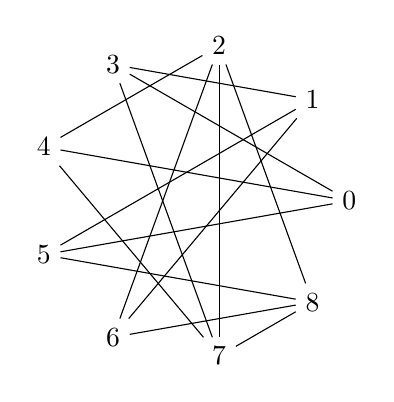
\begin{tikzpicture}
      \draw
        (0.0:2) node (0){0}
        (40.0:2) node (1){1}
        (80.0:2) node (2){2}
        (120.0:2) node (3){3}
        (160.0:2) node (4){4}
        (200.0:2) node (5){5}
        (240.0:2) node (6){6}
        (280.0:2) node (7){7}
        (320.0:2) node (8){8};
      \begin{scope}[-]
        \draw (0) to (3);
        \draw (0) to (4);
        \draw (0) to (5);
        \draw (1) to (3);
        \draw (1) to (5);
        \draw (1) to (6);
        \draw (2) to (4);
        \draw (2) to (6);
        \draw (2) to (7);
        \draw (2) to (8);
        \draw (3) to (7);
        \draw (4) to (7);
        \draw (5) to (8);
        \draw (6) to (8);
        \draw (7) to (8);
      \end{scope}
    \end{tikzpicture}
\end{figure}
\begin{itemize}
\item signature: 001110000101100010111000100010001011
\item g: Graph with 9 nodes and 15 edges
\item order: 9
\item size: 15
\item max degree: 4
\item degrees: 3,3,3,3,3,3,4,4,4
\item is tree: 0
\item is bipartite: 0
\item has bridge: 0
\item is chordal: 0
\item is complete: 0
\item min cycle basis weight: 26
\item min cycle basis size: 7
\item diameter: 3
\item radius: 2
\item is eulerian: 0
\item is planar: 0
\item number of faces: 8
\item is regular: 0
\item p3: 27
\item p4: 38
\item property hash: 5870bf19021d74c95162704bb5bd23e0eaf646bb74b2d40e7a305e46d6d0889a
\end{itemize}
\newpage
\begin{figure}
  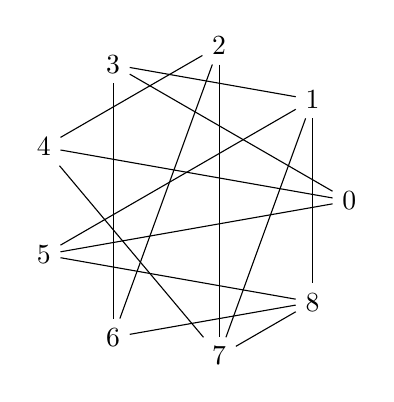
\begin{tikzpicture}
      \draw
        (0.0:2) node (0){0}
        (40.0:2) node (1){1}
        (80.0:2) node (2){2}
        (120.0:2) node (3){3}
        (160.0:2) node (4){4}
        (200.0:2) node (5){5}
        (240.0:2) node (6){6}
        (280.0:2) node (7){7}
        (320.0:2) node (8){8};
      \begin{scope}[-]
        \draw (0) to (3);
        \draw (0) to (4);
        \draw (0) to (5);
        \draw (1) to (3);
        \draw (1) to (5);
        \draw (1) to (7);
        \draw (1) to (8);
        \draw (2) to (4);
        \draw (2) to (6);
        \draw (2) to (7);
        \draw (3) to (6);
        \draw (4) to (7);
        \draw (5) to (8);
        \draw (6) to (8);
        \draw (7) to (8);
      \end{scope}
    \end{tikzpicture}
\end{figure}
\begin{itemize}
\item signature: 001110000101011010110001000010001011
\item g: Graph with 9 nodes and 15 edges
\item order: 9
\item size: 15
\item max degree: 4
\item degrees: 3,3,3,3,3,3,4,4,4
\item is tree: 0
\item is bipartite: 0
\item has bridge: 0
\item is chordal: 0
\item is complete: 0
\item min cycle basis weight: 26
\item min cycle basis size: 7
\item diameter: 3
\item radius: 2
\item is eulerian: 0
\item is planar: 0
\item number of faces: 8
\item is regular: 0
\item p3: 27
\item p4: 38
\item property hash: 5870bf19021d74c95162704bb5bd23e0eaf646bb74b2d40e7a305e46d6d0889a
\end{itemize}
\newpage
\begin{figure}
  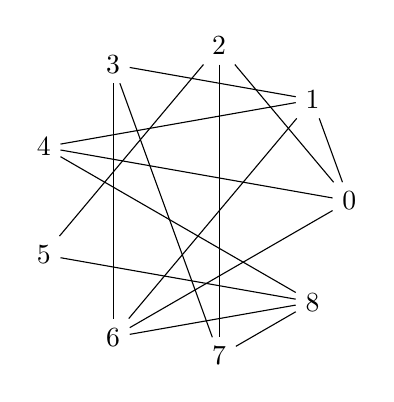
\begin{tikzpicture}
      \draw
        (0.0:2) node (0){0}
        (40.0:2) node (1){1}
        (80.0:2) node (2){2}
        (120.0:2) node (3){3}
        (160.0:2) node (4){4}
        (200.0:2) node (5){5}
        (240.0:2) node (6){6}
        (280.0:2) node (7){7}
        (320.0:2) node (8){8};
      \begin{scope}[-]
        \draw (0) to (1);
        \draw (0) to (2);
        \draw (0) to (4);
        \draw (0) to (6);
        \draw (1) to (3);
        \draw (1) to (4);
        \draw (1) to (6);
        \draw (2) to (5);
        \draw (2) to (7);
        \draw (3) to (6);
        \draw (3) to (7);
        \draw (4) to (8);
        \draw (5) to (8);
        \draw (6) to (8);
        \draw (7) to (8);
      \end{scope}
    \end{tikzpicture}
\end{figure}
\begin{itemize}
\item signature: 110101000110100001010001100001001011
\item g: Graph with 9 nodes and 15 edges
\item order: 9
\item size: 15
\item max degree: 4
\item degrees: 2,3,3,3,3,4,4,4,4
\item is tree: 0
\item is bipartite: 0
\item has bridge: 0
\item is chordal: 0
\item is complete: 0
\item min cycle basis weight: 26
\item min cycle basis size: 7
\item diameter: 3
\item radius: 2
\item is eulerian: 0
\item is planar: 0
\item number of faces: 8
\item is regular: 0
\item p3: 28
\item p4: 38
\item property hash: 28e5be1d3cffc9e665a481ab5ab0f04fb76b570011de23a07cfe2477e9bace79
\end{itemize}
\newpage
\begin{figure}
  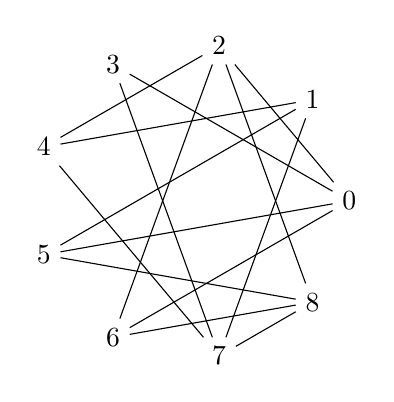
\begin{tikzpicture}
      \draw
        (0.0:2) node (0){0}
        (40.0:2) node (1){1}
        (80.0:2) node (2){2}
        (120.0:2) node (3){3}
        (160.0:2) node (4){4}
        (200.0:2) node (5){5}
        (240.0:2) node (6){6}
        (280.0:2) node (7){7}
        (320.0:2) node (8){8};
      \begin{scope}[-]
        \draw (0) to (2);
        \draw (0) to (3);
        \draw (0) to (5);
        \draw (0) to (6);
        \draw (1) to (4);
        \draw (1) to (5);
        \draw (1) to (7);
        \draw (2) to (4);
        \draw (2) to (6);
        \draw (2) to (8);
        \draw (3) to (7);
        \draw (4) to (7);
        \draw (5) to (8);
        \draw (6) to (8);
        \draw (7) to (8);
      \end{scope}
    \end{tikzpicture}
\end{figure}
\begin{itemize}
\item signature: 011011000011010010101000100010001011
\item g: Graph with 9 nodes and 15 edges
\item order: 9
\item size: 15
\item max degree: 4
\item degrees: 2,3,3,3,3,4,4,4,4
\item is tree: 0
\item is bipartite: 0
\item has bridge: 0
\item is chordal: 0
\item is complete: 0
\item min cycle basis weight: 26
\item min cycle basis size: 7
\item diameter: 3
\item radius: 2
\item is eulerian: 0
\item is planar: 0
\item number of faces: 8
\item is regular: 0
\item p3: 28
\item p4: 38
\item property hash: 28e5be1d3cffc9e665a481ab5ab0f04fb76b570011de23a07cfe2477e9bace79
\end{itemize}
\newpage
\begin{figure}
  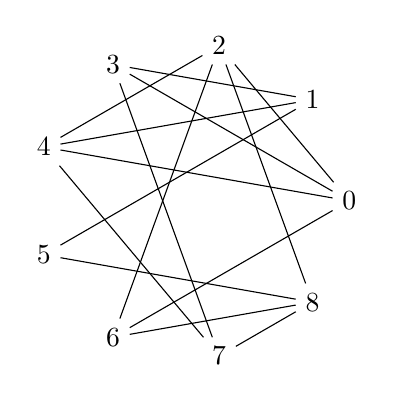
\begin{tikzpicture}
      \draw
        (0.0:2) node (0){0}
        (40.0:2) node (1){1}
        (80.0:2) node (2){2}
        (120.0:2) node (3){3}
        (160.0:2) node (4){4}
        (200.0:2) node (5){5}
        (240.0:2) node (6){6}
        (280.0:2) node (7){7}
        (320.0:2) node (8){8};
      \begin{scope}[-]
        \draw (0) to (2);
        \draw (0) to (3);
        \draw (0) to (4);
        \draw (0) to (6);
        \draw (1) to (3);
        \draw (1) to (4);
        \draw (1) to (5);
        \draw (2) to (4);
        \draw (2) to (6);
        \draw (2) to (8);
        \draw (3) to (7);
        \draw (4) to (7);
        \draw (5) to (8);
        \draw (6) to (8);
        \draw (7) to (8);
      \end{scope}
    \end{tikzpicture}
\end{figure}
\begin{itemize}
\item signature: 011101000111000010101000100010001011
\item g: Graph with 9 nodes and 15 edges
\item order: 9
\item size: 15
\item max degree: 4
\item degrees: 2,3,3,3,3,4,4,4,4
\item is tree: 0
\item is bipartite: 0
\item has bridge: 0
\item is chordal: 0
\item is complete: 0
\item min cycle basis weight: 26
\item min cycle basis size: 7
\item diameter: 3
\item radius: 2
\item is eulerian: 0
\item is planar: 0
\item number of faces: 8
\item is regular: 0
\item p3: 28
\item p4: 38
\item property hash: 28e5be1d3cffc9e665a481ab5ab0f04fb76b570011de23a07cfe2477e9bace79
\end{itemize}
\newpage
\begin{figure}
  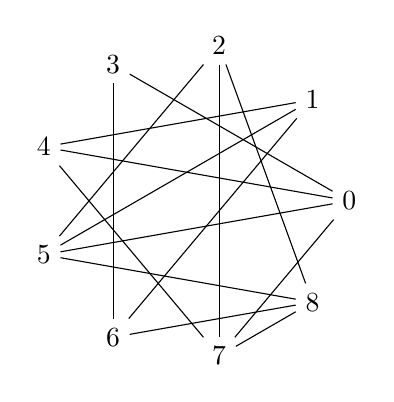
\begin{tikzpicture}
      \draw
        (0.0:2) node (0){0}
        (40.0:2) node (1){1}
        (80.0:2) node (2){2}
        (120.0:2) node (3){3}
        (160.0:2) node (4){4}
        (200.0:2) node (5){5}
        (240.0:2) node (6){6}
        (280.0:2) node (7){7}
        (320.0:2) node (8){8};
      \begin{scope}[-]
        \draw (0) to (3);
        \draw (0) to (4);
        \draw (0) to (5);
        \draw (0) to (7);
        \draw (1) to (4);
        \draw (1) to (5);
        \draw (1) to (6);
        \draw (2) to (5);
        \draw (2) to (7);
        \draw (2) to (8);
        \draw (3) to (6);
        \draw (4) to (7);
        \draw (5) to (8);
        \draw (6) to (8);
        \draw (7) to (8);
      \end{scope}
    \end{tikzpicture}
\end{figure}
\begin{itemize}
\item signature: 001110100011100001011001000010001011
\item g: Graph with 9 nodes and 15 edges
\item order: 9
\item size: 15
\item max degree: 4
\item degrees: 2,3,3,3,3,4,4,4,4
\item is tree: 0
\item is bipartite: 0
\item has bridge: 0
\item is chordal: 0
\item is complete: 0
\item min cycle basis weight: 26
\item min cycle basis size: 7
\item diameter: 3
\item radius: 2
\item is eulerian: 0
\item is planar: 0
\item number of faces: 8
\item is regular: 0
\item p3: 28
\item p4: 38
\item property hash: 28e5be1d3cffc9e665a481ab5ab0f04fb76b570011de23a07cfe2477e9bace79
\end{itemize}
\newpage
\begin{figure}
  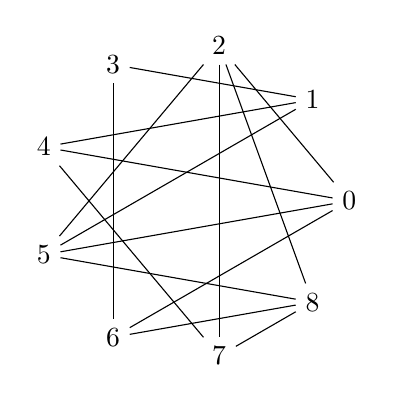
\begin{tikzpicture}
      \draw
        (0.0:2) node (0){0}
        (40.0:2) node (1){1}
        (80.0:2) node (2){2}
        (120.0:2) node (3){3}
        (160.0:2) node (4){4}
        (200.0:2) node (5){5}
        (240.0:2) node (6){6}
        (280.0:2) node (7){7}
        (320.0:2) node (8){8};
      \begin{scope}[-]
        \draw (0) to (2);
        \draw (0) to (4);
        \draw (0) to (5);
        \draw (0) to (6);
        \draw (1) to (3);
        \draw (1) to (4);
        \draw (1) to (5);
        \draw (2) to (5);
        \draw (2) to (7);
        \draw (2) to (8);
        \draw (3) to (6);
        \draw (4) to (7);
        \draw (5) to (8);
        \draw (6) to (8);
        \draw (7) to (8);
      \end{scope}
    \end{tikzpicture}
\end{figure}
\begin{itemize}
\item signature: 010111000111000001011001000010001011
\item g: Graph with 9 nodes and 15 edges
\item order: 9
\item size: 15
\item max degree: 4
\item degrees: 2,3,3,3,3,4,4,4,4
\item is tree: 0
\item is bipartite: 0
\item has bridge: 0
\item is chordal: 0
\item is complete: 0
\item min cycle basis weight: 26
\item min cycle basis size: 7
\item diameter: 3
\item radius: 2
\item is eulerian: 0
\item is planar: 0
\item number of faces: 8
\item is regular: 0
\item p3: 28
\item p4: 38
\item property hash: 28e5be1d3cffc9e665a481ab5ab0f04fb76b570011de23a07cfe2477e9bace79
\end{itemize}
\newpage
\begin{figure}
  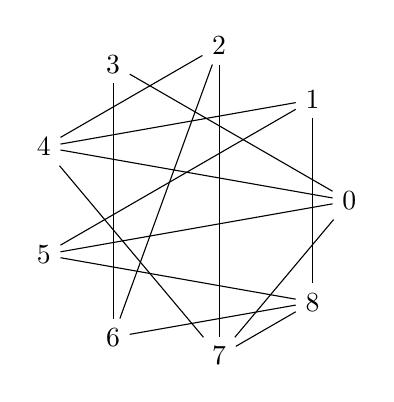
\begin{tikzpicture}
      \draw
        (0.0:2) node (0){0}
        (40.0:2) node (1){1}
        (80.0:2) node (2){2}
        (120.0:2) node (3){3}
        (160.0:2) node (4){4}
        (200.0:2) node (5){5}
        (240.0:2) node (6){6}
        (280.0:2) node (7){7}
        (320.0:2) node (8){8};
      \begin{scope}[-]
        \draw (0) to (3);
        \draw (0) to (4);
        \draw (0) to (5);
        \draw (0) to (7);
        \draw (1) to (4);
        \draw (1) to (5);
        \draw (1) to (8);
        \draw (2) to (4);
        \draw (2) to (6);
        \draw (2) to (7);
        \draw (3) to (6);
        \draw (4) to (7);
        \draw (5) to (8);
        \draw (6) to (8);
        \draw (7) to (8);
      \end{scope}
    \end{tikzpicture}
\end{figure}
\begin{itemize}
\item signature: 001110100011001010110001000010001011
\item g: Graph with 9 nodes and 15 edges
\item order: 9
\item size: 15
\item max degree: 4
\item degrees: 2,3,3,3,3,4,4,4,4
\item is tree: 0
\item is bipartite: 0
\item has bridge: 0
\item is chordal: 0
\item is complete: 0
\item min cycle basis weight: 26
\item min cycle basis size: 7
\item diameter: 3
\item radius: 2
\item is eulerian: 0
\item is planar: 0
\item number of faces: 8
\item is regular: 0
\item p3: 28
\item p4: 38
\item property hash: 28e5be1d3cffc9e665a481ab5ab0f04fb76b570011de23a07cfe2477e9bace79
\end{itemize}
\newpage
\begin{figure}
  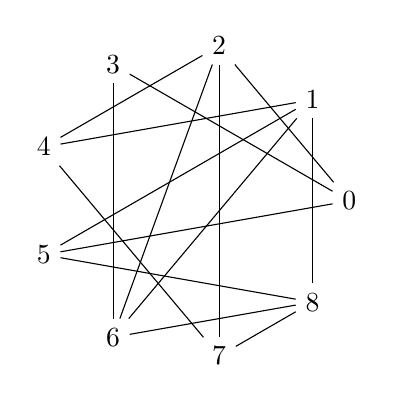
\begin{tikzpicture}
      \draw
        (0.0:2) node (0){0}
        (40.0:2) node (1){1}
        (80.0:2) node (2){2}
        (120.0:2) node (3){3}
        (160.0:2) node (4){4}
        (200.0:2) node (5){5}
        (240.0:2) node (6){6}
        (280.0:2) node (7){7}
        (320.0:2) node (8){8};
      \begin{scope}[-]
        \draw (0) to (2);
        \draw (0) to (3);
        \draw (0) to (5);
        \draw (1) to (4);
        \draw (1) to (5);
        \draw (1) to (6);
        \draw (1) to (8);
        \draw (2) to (4);
        \draw (2) to (6);
        \draw (2) to (7);
        \draw (3) to (6);
        \draw (4) to (7);
        \draw (5) to (8);
        \draw (6) to (8);
        \draw (7) to (8);
      \end{scope}
    \end{tikzpicture}
\end{figure}
\begin{itemize}
\item signature: 011010000011101010110001000010001011
\item g: Graph with 9 nodes and 15 edges
\item order: 9
\item size: 15
\item max degree: 4
\item degrees: 2,3,3,3,3,4,4,4,4
\item is tree: 0
\item is bipartite: 0
\item has bridge: 0
\item is chordal: 0
\item is complete: 0
\item min cycle basis weight: 26
\item min cycle basis size: 7
\item diameter: 3
\item radius: 2
\item is eulerian: 0
\item is planar: 0
\item number of faces: 8
\item is regular: 0
\item p3: 28
\item p4: 38
\item property hash: 28e5be1d3cffc9e665a481ab5ab0f04fb76b570011de23a07cfe2477e9bace79
\end{itemize}
\newpage
\begin{figure}
  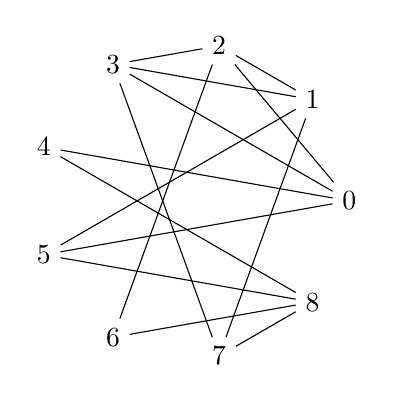
\begin{tikzpicture}
      \draw
        (0.0:2) node (0){0}
        (40.0:2) node (1){1}
        (80.0:2) node (2){2}
        (120.0:2) node (3){3}
        (160.0:2) node (4){4}
        (200.0:2) node (5){5}
        (240.0:2) node (6){6}
        (280.0:2) node (7){7}
        (320.0:2) node (8){8};
      \begin{scope}[-]
        \draw (0) to (2);
        \draw (0) to (3);
        \draw (0) to (4);
        \draw (0) to (5);
        \draw (1) to (2);
        \draw (1) to (3);
        \draw (1) to (5);
        \draw (1) to (7);
        \draw (2) to (3);
        \draw (2) to (6);
        \draw (3) to (7);
        \draw (4) to (8);
        \draw (5) to (8);
        \draw (6) to (8);
        \draw (7) to (8);
      \end{scope}
    \end{tikzpicture}
\end{figure}
\begin{itemize}
\item signature: 011110001101010100100000100001001011
\item g: Graph with 9 nodes and 15 edges
\item order: 9
\item size: 15
\item max degree: 4
\item degrees: 2,2,3,3,4,4,4,4,4
\item is tree: 0
\item is bipartite: 0
\item has bridge: 0
\item is chordal: 0
\item is complete: 0
\item min cycle basis weight: 26
\item min cycle basis size: 7
\item diameter: 3
\item radius: 2
\item is eulerian: 0
\item is planar: 0
\item number of faces: 8
\item is regular: 0
\item p3: 29
\item p4: 38
\item property hash: 0590187412025eb3a94580a51f11c618dca7b6f5400f5245eb1c1513c6524163
\end{itemize}
\newpage
\begin{figure}
  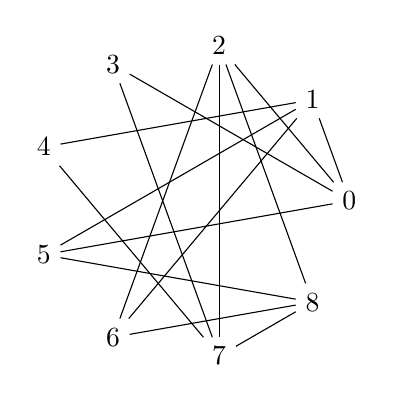
\begin{tikzpicture}
      \draw
        (0.0:2) node (0){0}
        (40.0:2) node (1){1}
        (80.0:2) node (2){2}
        (120.0:2) node (3){3}
        (160.0:2) node (4){4}
        (200.0:2) node (5){5}
        (240.0:2) node (6){6}
        (280.0:2) node (7){7}
        (320.0:2) node (8){8};
      \begin{scope}[-]
        \draw (0) to (1);
        \draw (0) to (2);
        \draw (0) to (3);
        \draw (0) to (5);
        \draw (1) to (4);
        \draw (1) to (5);
        \draw (1) to (6);
        \draw (2) to (6);
        \draw (2) to (7);
        \draw (2) to (8);
        \draw (3) to (7);
        \draw (4) to (7);
        \draw (5) to (8);
        \draw (6) to (8);
        \draw (7) to (8);
      \end{scope}
    \end{tikzpicture}
\end{figure}
\begin{itemize}
\item signature: 111010000011100000111000100010001011
\item g: Graph with 9 nodes and 15 edges
\item order: 9
\item size: 15
\item max degree: 4
\item degrees: 2,2,3,3,4,4,4,4,4
\item is tree: 0
\item is bipartite: 0
\item has bridge: 0
\item is chordal: 0
\item is complete: 0
\item min cycle basis weight: 26
\item min cycle basis size: 7
\item diameter: 3
\item radius: 2
\item is eulerian: 0
\item is planar: 0
\item number of faces: 8
\item is regular: 0
\item p3: 29
\item p4: 38
\item property hash: 0590187412025eb3a94580a51f11c618dca7b6f5400f5245eb1c1513c6524163
\end{itemize}
\newpage
\begin{figure}
  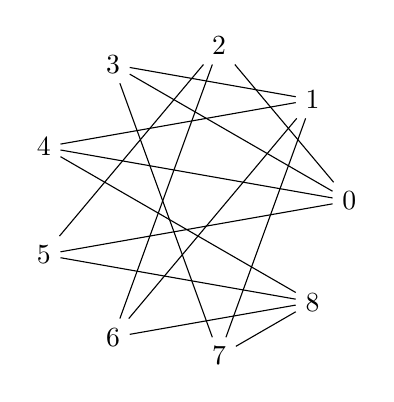
\begin{tikzpicture}
      \draw
        (0.0:2) node (0){0}
        (40.0:2) node (1){1}
        (80.0:2) node (2){2}
        (120.0:2) node (3){3}
        (160.0:2) node (4){4}
        (200.0:2) node (5){5}
        (240.0:2) node (6){6}
        (280.0:2) node (7){7}
        (320.0:2) node (8){8};
      \begin{scope}[-]
        \draw (0) to (2);
        \draw (0) to (3);
        \draw (0) to (4);
        \draw (0) to (5);
        \draw (1) to (3);
        \draw (1) to (4);
        \draw (1) to (6);
        \draw (1) to (7);
        \draw (2) to (5);
        \draw (2) to (6);
        \draw (3) to (7);
        \draw (4) to (8);
        \draw (5) to (8);
        \draw (6) to (8);
        \draw (7) to (8);
      \end{scope}
    \end{tikzpicture}
\end{figure}
\begin{itemize}
\item signature: 011110000110110001100000100001001011
\item g: Graph with 9 nodes and 15 edges
\item order: 9
\item size: 15
\item max degree: 4
\item degrees: 3,3,3,3,3,3,4,4,4
\item is tree: 0
\item is bipartite: 0
\item has bridge: 0
\item is chordal: 0
\item is complete: 0
\item min cycle basis weight: 26
\item min cycle basis size: 7
\item diameter: 3
\item radius: 2
\item is eulerian: 0
\item is planar: 0
\item number of faces: 8
\item is regular: 0
\item p3: 30
\item p4: 38
\item property hash: 8c7c5cc8232a058e5f462c6061cd4af67a4e4ed5c79fc5d60757065193654563
\end{itemize}
\newpage
\begin{figure}
  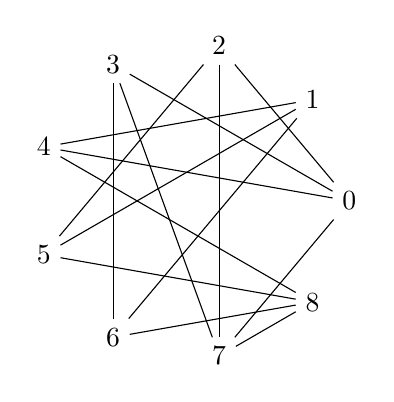
\begin{tikzpicture}
      \draw
        (0.0:2) node (0){0}
        (40.0:2) node (1){1}
        (80.0:2) node (2){2}
        (120.0:2) node (3){3}
        (160.0:2) node (4){4}
        (200.0:2) node (5){5}
        (240.0:2) node (6){6}
        (280.0:2) node (7){7}
        (320.0:2) node (8){8};
      \begin{scope}[-]
        \draw (0) to (2);
        \draw (0) to (3);
        \draw (0) to (4);
        \draw (0) to (7);
        \draw (1) to (4);
        \draw (1) to (5);
        \draw (1) to (6);
        \draw (2) to (5);
        \draw (2) to (7);
        \draw (3) to (6);
        \draw (3) to (7);
        \draw (4) to (8);
        \draw (5) to (8);
        \draw (6) to (8);
        \draw (7) to (8);
      \end{scope}
    \end{tikzpicture}
\end{figure}
\begin{itemize}
\item signature: 011100100011100001010001100001001011
\item g: Graph with 9 nodes and 15 edges
\item order: 9
\item size: 15
\item max degree: 4
\item degrees: 3,3,3,3,3,3,4,4,4
\item is tree: 0
\item is bipartite: 0
\item has bridge: 0
\item is chordal: 0
\item is complete: 0
\item min cycle basis weight: 26
\item min cycle basis size: 7
\item diameter: 3
\item radius: 2
\item is eulerian: 0
\item is planar: 0
\item number of faces: 8
\item is regular: 0
\item p3: 30
\item p4: 38
\item property hash: 8c7c5cc8232a058e5f462c6061cd4af67a4e4ed5c79fc5d60757065193654563
\end{itemize}
\newpage
\begin{figure}
  \begin{tikzpicture}
      \draw
        (0.0:2) node (0){0}
        (40.0:2) node (1){1}
        (80.0:2) node (2){2}
        (120.0:2) node (3){3}
        (160.0:2) node (4){4}
        (200.0:2) node (5){5}
        (240.0:2) node (6){6}
        (280.0:2) node (7){7}
        (320.0:2) node (8){8};
      \begin{scope}[-]
        \draw (0) to (3);
        \draw (0) to (4);
        \draw (0) to (5);
        \draw (1) to (3);
        \draw (1) to (5);
        \draw (1) to (6);
        \draw (1) to (7);
        \draw (2) to (4);
        \draw (2) to (6);
        \draw (2) to (8);
        \draw (3) to (7);
        \draw (4) to (7);
        \draw (5) to (8);
        \draw (6) to (8);
        \draw (7) to (8);
      \end{scope}
    \end{tikzpicture}
\end{figure}
\begin{itemize}
\item signature: 001110000101110010101000100010001011
\item g: Graph with 9 nodes and 15 edges
\item order: 9
\item size: 15
\item max degree: 4
\item degrees: 3,3,3,3,3,3,4,4,4
\item is tree: 0
\item is bipartite: 0
\item has bridge: 0
\item is chordal: 0
\item is complete: 0
\item min cycle basis weight: 26
\item min cycle basis size: 7
\item diameter: 3
\item radius: 2
\item is eulerian: 0
\item is planar: 0
\item number of faces: 8
\item is regular: 0
\item p3: 30
\item p4: 38
\item property hash: 8c7c5cc8232a058e5f462c6061cd4af67a4e4ed5c79fc5d60757065193654563
\end{itemize}
\newpage
\begin{figure}
  \begin{tikzpicture}
      \draw
        (0.0:2) node (0){0}
        (40.0:2) node (1){1}
        (80.0:2) node (2){2}
        (120.0:2) node (3){3}
        (160.0:2) node (4){4}
        (200.0:2) node (5){5}
        (240.0:2) node (6){6}
        (280.0:2) node (7){7}
        (320.0:2) node (8){8};
      \begin{scope}[-]
        \draw (0) to (2);
        \draw (0) to (3);
        \draw (0) to (4);
        \draw (0) to (6);
        \draw (1) to (4);
        \draw (1) to (5);
        \draw (1) to (6);
        \draw (2) to (5);
        \draw (2) to (6);
        \draw (3) to (7);
        \draw (3) to (8);
        \draw (4) to (7);
        \draw (5) to (8);
        \draw (6) to (8);
        \draw (7) to (8);
      \end{scope}
    \end{tikzpicture}
\end{figure}
\begin{itemize}
\item signature: 011101000011100001100000110010001011
\item g: Graph with 9 nodes and 15 edges
\item order: 9
\item size: 15
\item max degree: 4
\item degrees: 3,3,3,3,3,3,4,4,4
\item is tree: 0
\item is bipartite: 0
\item has bridge: 0
\item is chordal: 0
\item is complete: 0
\item min cycle basis weight: 26
\item min cycle basis size: 7
\item diameter: 3
\item radius: 2
\item is eulerian: 0
\item is planar: 0
\item number of faces: 8
\item is regular: 0
\item p3: 30
\item p4: 38
\item property hash: 8c7c5cc8232a058e5f462c6061cd4af67a4e4ed5c79fc5d60757065193654563
\end{itemize}
\newpage
\begin{figure}
  \begin{tikzpicture}
      \draw
        (0.0:2) node (0){0}
        (40.0:2) node (1){1}
        (80.0:2) node (2){2}
        (120.0:2) node (3){3}
        (160.0:2) node (4){4}
        (200.0:2) node (5){5}
        (240.0:2) node (6){6}
        (280.0:2) node (7){7}
        (320.0:2) node (8){8};
      \begin{scope}[-]
        \draw (0) to (1);
        \draw (0) to (2);
        \draw (0) to (3);
        \draw (0) to (5);
        \draw (1) to (3);
        \draw (1) to (4);
        \draw (1) to (6);
        \draw (2) to (5);
        \draw (2) to (6);
        \draw (2) to (7);
        \draw (3) to (7);
        \draw (4) to (8);
        \draw (5) to (8);
        \draw (6) to (8);
        \draw (7) to (8);
      \end{scope}
    \end{tikzpicture}
\end{figure}
\begin{itemize}
\item signature: 111010000110100001110000100001001011
\item g: Graph with 9 nodes and 15 edges
\item order: 9
\item size: 15
\item max degree: 4
\item degrees: 2,3,3,3,3,4,4,4,4
\item is tree: 0
\item is bipartite: 0
\item has bridge: 0
\item is chordal: 0
\item is complete: 0
\item min cycle basis weight: 26
\item min cycle basis size: 7
\item diameter: 3
\item radius: 2
\item is eulerian: 0
\item is planar: 0
\item number of faces: 8
\item is regular: 0
\item p3: 31
\item p4: 38
\item property hash: 701c0242bd57366f9df8b31767ab312b8952b7863b27ec3e601b92a69d1795e5
\end{itemize}
\newpage
\begin{figure}
  \begin{tikzpicture}
      \draw
        (0.0:2) node (0){0}
        (40.0:2) node (1){1}
        (80.0:2) node (2){2}
        (120.0:2) node (3){3}
        (160.0:2) node (4){4}
        (200.0:2) node (5){5}
        (240.0:2) node (6){6}
        (280.0:2) node (7){7}
        (320.0:2) node (8){8};
      \begin{scope}[-]
        \draw (0) to (2);
        \draw (0) to (4);
        \draw (0) to (6);
        \draw (0) to (7);
        \draw (1) to (3);
        \draw (1) to (5);
        \draw (1) to (6);
        \draw (2) to (5);
        \draw (2) to (7);
        \draw (3) to (6);
        \draw (3) to (7);
        \draw (4) to (8);
        \draw (5) to (8);
        \draw (6) to (8);
        \draw (7) to (8);
      \end{scope}
    \end{tikzpicture}
\end{figure}
\begin{itemize}
\item signature: 010101100101100001010001100001001011
\item g: Graph with 9 nodes and 15 edges
\item order: 9
\item size: 15
\item max degree: 4
\item degrees: 2,3,3,3,3,4,4,4,4
\item is tree: 0
\item is bipartite: 0
\item has bridge: 0
\item is chordal: 0
\item is complete: 0
\item min cycle basis weight: 26
\item min cycle basis size: 7
\item diameter: 3
\item radius: 2
\item is eulerian: 0
\item is planar: 0
\item number of faces: 8
\item is regular: 0
\item p3: 31
\item p4: 38
\item property hash: 701c0242bd57366f9df8b31767ab312b8952b7863b27ec3e601b92a69d1795e5
\end{itemize}
\newpage
\begin{figure}
  \begin{tikzpicture}
      \draw
        (0.0:2) node (0){0}
        (40.0:2) node (1){1}
        (80.0:2) node (2){2}
        (120.0:2) node (3){3}
        (160.0:2) node (4){4}
        (200.0:2) node (5){5}
        (240.0:2) node (6){6}
        (280.0:2) node (7){7}
        (320.0:2) node (8){8};
      \begin{scope}[-]
        \draw (0) to (2);
        \draw (0) to (3);
        \draw (0) to (4);
        \draw (0) to (5);
        \draw (1) to (4);
        \draw (1) to (5);
        \draw (1) to (6);
        \draw (1) to (7);
        \draw (2) to (4);
        \draw (2) to (6);
        \draw (3) to (7);
        \draw (4) to (7);
        \draw (5) to (8);
        \draw (6) to (8);
        \draw (7) to (8);
      \end{scope}
    \end{tikzpicture}
\end{figure}
\begin{itemize}
\item signature: 011110000011110010100000100010001011
\item g: Graph with 9 nodes and 15 edges
\item order: 9
\item size: 15
\item max degree: 4
\item degrees: 2,3,3,3,3,4,4,4,4
\item is tree: 0
\item is bipartite: 0
\item has bridge: 0
\item is chordal: 0
\item is complete: 0
\item min cycle basis weight: 26
\item min cycle basis size: 7
\item diameter: 3
\item radius: 2
\item is eulerian: 0
\item is planar: 0
\item number of faces: 8
\item is regular: 0
\item p3: 31
\item p4: 38
\item property hash: 701c0242bd57366f9df8b31767ab312b8952b7863b27ec3e601b92a69d1795e5
\end{itemize}
\newpage
\begin{figure}
  \begin{tikzpicture}
      \draw
        (0.0:2) node (0){0}
        (40.0:2) node (1){1}
        (80.0:2) node (2){2}
        (120.0:2) node (3){3}
        (160.0:2) node (4){4}
        (200.0:2) node (5){5}
        (240.0:2) node (6){6}
        (280.0:2) node (7){7}
        (320.0:2) node (8){8};
      \begin{scope}[-]
        \draw (0) to (3);
        \draw (0) to (5);
        \draw (0) to (6);
        \draw (0) to (7);
        \draw (1) to (4);
        \draw (1) to (5);
        \draw (1) to (6);
        \draw (2) to (4);
        \draw (2) to (6);
        \draw (2) to (8);
        \draw (3) to (7);
        \draw (4) to (7);
        \draw (5) to (8);
        \draw (6) to (8);
        \draw (7) to (8);
      \end{scope}
    \end{tikzpicture}
\end{figure}
\begin{itemize}
\item signature: 001011100011100010101000100010001011
\item g: Graph with 9 nodes and 15 edges
\item order: 9
\item size: 15
\item max degree: 4
\item degrees: 2,3,3,3,3,4,4,4,4
\item is tree: 0
\item is bipartite: 0
\item has bridge: 0
\item is chordal: 0
\item is complete: 0
\item min cycle basis weight: 26
\item min cycle basis size: 7
\item diameter: 3
\item radius: 2
\item is eulerian: 0
\item is planar: 0
\item number of faces: 8
\item is regular: 0
\item p3: 31
\item p4: 38
\item property hash: 701c0242bd57366f9df8b31767ab312b8952b7863b27ec3e601b92a69d1795e5
\end{itemize}
\newpage
\begin{figure}
  \begin{tikzpicture}
      \draw
        (0.0:2) node (0){0}
        (40.0:2) node (1){1}
        (80.0:2) node (2){2}
        (120.0:2) node (3){3}
        (160.0:2) node (4){4}
        (200.0:2) node (5){5}
        (240.0:2) node (6){6}
        (280.0:2) node (7){7}
        (320.0:2) node (8){8};
      \begin{scope}[-]
        \draw (0) to (2);
        \draw (0) to (3);
        \draw (0) to (5);
        \draw (0) to (7);
        \draw (1) to (4);
        \draw (1) to (5);
        \draw (1) to (6);
        \draw (2) to (4);
        \draw (2) to (6);
        \draw (2) to (8);
        \draw (3) to (7);
        \draw (4) to (7);
        \draw (5) to (8);
        \draw (6) to (8);
        \draw (7) to (8);
      \end{scope}
    \end{tikzpicture}
\end{figure}
\begin{itemize}
\item signature: 011010100011100010101000100010001011
\item g: Graph with 9 nodes and 15 edges
\item order: 9
\item size: 15
\item max degree: 4
\item degrees: 2,3,3,3,3,4,4,4,4
\item is tree: 0
\item is bipartite: 0
\item has bridge: 0
\item is chordal: 0
\item is complete: 0
\item min cycle basis weight: 26
\item min cycle basis size: 7
\item diameter: 3
\item radius: 2
\item is eulerian: 0
\item is planar: 0
\item number of faces: 8
\item is regular: 0
\item p3: 31
\item p4: 38
\item property hash: 701c0242bd57366f9df8b31767ab312b8952b7863b27ec3e601b92a69d1795e5
\end{itemize}
\newpage
\begin{figure}
  \begin{tikzpicture}
      \draw
        (0.0:2) node (0){0}
        (40.0:2) node (1){1}
        (80.0:2) node (2){2}
        (120.0:2) node (3){3}
        (160.0:2) node (4){4}
        (200.0:2) node (5){5}
        (240.0:2) node (6){6}
        (280.0:2) node (7){7}
        (320.0:2) node (8){8};
      \begin{scope}[-]
        \draw (0) to (1);
        \draw (0) to (2);
        \draw (0) to (3);
        \draw (0) to (4);
        \draw (1) to (4);
        \draw (1) to (5);
        \draw (1) to (6);
        \draw (2) to (6);
        \draw (2) to (7);
        \draw (3) to (7);
        \draw (3) to (8);
        \draw (4) to (7);
        \draw (5) to (8);
        \draw (6) to (8);
        \draw (7) to (8);
      \end{scope}
    \end{tikzpicture}
\end{figure}
\begin{itemize}
\item signature: 111100000011100000110000110010001011
\item g: Graph with 9 nodes and 15 edges
\item order: 9
\item size: 15
\item max degree: 4
\item degrees: 2,3,3,3,3,4,4,4,4
\item is tree: 0
\item is bipartite: 0
\item has bridge: 0
\item is chordal: 0
\item is complete: 0
\item min cycle basis weight: 26
\item min cycle basis size: 7
\item diameter: 3
\item radius: 2
\item is eulerian: 0
\item is planar: 0
\item number of faces: 8
\item is regular: 0
\item p3: 31
\item p4: 38
\item property hash: 701c0242bd57366f9df8b31767ab312b8952b7863b27ec3e601b92a69d1795e5
\end{itemize}
\newpage
\begin{figure}
  \begin{tikzpicture}
      \draw
        (0.0:2) node (0){0}
        (40.0:2) node (1){1}
        (80.0:2) node (2){2}
        (120.0:2) node (3){3}
        (160.0:2) node (4){4}
        (200.0:2) node (5){5}
        (240.0:2) node (6){6}
        (280.0:2) node (7){7}
        (320.0:2) node (8){8};
      \begin{scope}[-]
        \draw (0) to (2);
        \draw (0) to (3);
        \draw (0) to (4);
        \draw (0) to (6);
        \draw (1) to (2);
        \draw (1) to (3);
        \draw (1) to (5);
        \draw (1) to (6);
        \draw (2) to (6);
        \draw (2) to (7);
        \draw (3) to (7);
        \draw (4) to (8);
        \draw (5) to (8);
        \draw (6) to (8);
        \draw (7) to (8);
      \end{scope}
    \end{tikzpicture}
\end{figure}
\begin{itemize}
\item signature: 011101001101100000110000100001001011
\item g: Graph with 9 nodes and 15 edges
\item order: 9
\item size: 15
\item max degree: 4
\item degrees: 2,2,3,3,4,4,4,4,4
\item is tree: 0
\item is bipartite: 0
\item has bridge: 0
\item is chordal: 0
\item is complete: 0
\item min cycle basis weight: 26
\item min cycle basis size: 7
\item diameter: 3
\item radius: 2
\item is eulerian: 0
\item is planar: 0
\item number of faces: 8
\item is regular: 0
\item p3: 32
\item p4: 38
\item property hash: 57d326b814dbe8b31fcfa368375832aab30b33893b73ed6790c20bc7a77d31d3
\end{itemize}
\newpage
\begin{figure}
  \begin{tikzpicture}
      \draw
        (0.0:2) node (0){0}
        (40.0:2) node (1){1}
        (80.0:2) node (2){2}
        (120.0:2) node (3){3}
        (160.0:2) node (4){4}
        (200.0:2) node (5){5}
        (240.0:2) node (6){6}
        (280.0:2) node (7){7}
        (320.0:2) node (8){8};
      \begin{scope}[-]
        \draw (0) to (2);
        \draw (0) to (3);
        \draw (0) to (5);
        \draw (0) to (6);
        \draw (1) to (4);
        \draw (1) to (5);
        \draw (1) to (6);
        \draw (2) to (4);
        \draw (2) to (6);
        \draw (3) to (7);
        \draw (3) to (8);
        \draw (4) to (7);
        \draw (5) to (8);
        \draw (6) to (8);
        \draw (7) to (8);
      \end{scope}
    \end{tikzpicture}
\end{figure}
\begin{itemize}
\item signature: 011011000011100010100000110010001011
\item g: Graph with 9 nodes and 15 edges
\item order: 9
\item size: 15
\item max degree: 4
\item degrees: 3,3,3,3,3,3,4,4,4
\item is tree: 0
\item is bipartite: 0
\item has bridge: 0
\item is chordal: 0
\item is complete: 0
\item min cycle basis weight: 27
\item min cycle basis size: 7
\item diameter: 3
\item radius: 2
\item is eulerian: 0
\item is planar: 0
\item number of faces: 8
\item is regular: 0
\item p3: 30
\item p4: 38
\item property hash: bb5d56a439eb1da505304ee08808004d07ed2e3f54dbc0b52602095c9b5c9455
\end{itemize}
\newpage
\begin{figure}
  \begin{tikzpicture}
      \draw
        (0.0:2) node (0){0}
        (40.0:2) node (1){1}
        (80.0:2) node (2){2}
        (120.0:2) node (3){3}
        (160.0:2) node (4){4}
        (200.0:2) node (5){5}
        (240.0:2) node (6){6}
        (280.0:2) node (7){7}
        (320.0:2) node (8){8};
      \begin{scope}[-]
        \draw (0) to (2);
        \draw (0) to (3);
        \draw (0) to (4);
        \draw (0) to (5);
        \draw (1) to (3);
        \draw (1) to (5);
        \draw (1) to (6);
        \draw (2) to (4);
        \draw (2) to (6);
        \draw (3) to (7);
        \draw (3) to (8);
        \draw (4) to (7);
        \draw (5) to (8);
        \draw (6) to (8);
        \draw (7) to (8);
      \end{scope}
    \end{tikzpicture}
\end{figure}
\begin{itemize}
\item signature: 011110000101100010100000110010001011
\item g: Graph with 9 nodes and 15 edges
\item order: 9
\item size: 15
\item max degree: 4
\item degrees: 3,3,3,3,3,3,4,4,4
\item is tree: 0
\item is bipartite: 0
\item has bridge: 0
\item is chordal: 0
\item is complete: 0
\item min cycle basis weight: 27
\item min cycle basis size: 7
\item diameter: 3
\item radius: 2
\item is eulerian: 0
\item is planar: 0
\item number of faces: 8
\item is regular: 0
\item p3: 30
\item p4: 38
\item property hash: bb5d56a439eb1da505304ee08808004d07ed2e3f54dbc0b52602095c9b5c9455
\end{itemize}
\newpage
\begin{figure}
  \begin{tikzpicture}
      \draw
        (0.0:2) node (0){0}
        (40.0:2) node (1){1}
        (80.0:2) node (2){2}
        (120.0:2) node (3){3}
        (160.0:2) node (4){4}
        (200.0:2) node (5){5}
        (240.0:2) node (6){6}
        (280.0:2) node (7){7}
        (320.0:2) node (8){8};
      \begin{scope}[-]
        \draw (0) to (2);
        \draw (0) to (3);
        \draw (0) to (4);
        \draw (0) to (7);
        \draw (1) to (3);
        \draw (1) to (4);
        \draw (1) to (6);
        \draw (1) to (7);
        \draw (2) to (5);
        \draw (2) to (6);
        \draw (3) to (7);
        \draw (4) to (8);
        \draw (5) to (8);
        \draw (6) to (8);
        \draw (7) to (8);
      \end{scope}
    \end{tikzpicture}
\end{figure}
\begin{itemize}
\item signature: 011100100110110001100000100001001011
\item g: Graph with 9 nodes and 15 edges
\item order: 9
\item size: 15
\item max degree: 4
\item degrees: 2,3,3,3,3,4,4,4,4
\item is tree: 0
\item is bipartite: 0
\item has bridge: 0
\item is chordal: 0
\item is complete: 0
\item min cycle basis weight: 27
\item min cycle basis size: 7
\item diameter: 3
\item radius: 2
\item is eulerian: 0
\item is planar: 0
\item number of faces: 8
\item is regular: 0
\item p3: 31
\item p4: 38
\item property hash: 98eba25430a43f991981dc793e83c0b8929005668a1a8dcd0ea9e050bb2373fb
\end{itemize}
\newpage
\begin{figure}
  \begin{tikzpicture}
      \draw
        (0.0:2) node (0){0}
        (40.0:2) node (1){1}
        (80.0:2) node (2){2}
        (120.0:2) node (3){3}
        (160.0:2) node (4){4}
        (200.0:2) node (5){5}
        (240.0:2) node (6){6}
        (280.0:2) node (7){7}
        (320.0:2) node (8){8};
      \begin{scope}[-]
        \draw (0) to (2);
        \draw (0) to (3);
        \draw (0) to (7);
        \draw (1) to (3);
        \draw (1) to (4);
        \draw (1) to (5);
        \draw (1) to (6);
        \draw (2) to (5);
        \draw (2) to (6);
        \draw (2) to (7);
        \draw (3) to (7);
        \draw (4) to (8);
        \draw (5) to (8);
        \draw (6) to (8);
        \draw (7) to (8);
      \end{scope}
    \end{tikzpicture}
\end{figure}
\begin{itemize}
\item signature: 011000100111100001110000100001001011
\item g: Graph with 9 nodes and 15 edges
\item order: 9
\item size: 15
\item max degree: 4
\item degrees: 2,3,3,3,3,4,4,4,4
\item is tree: 0
\item is bipartite: 0
\item has bridge: 0
\item is chordal: 0
\item is complete: 0
\item min cycle basis weight: 27
\item min cycle basis size: 7
\item diameter: 3
\item radius: 2
\item is eulerian: 0
\item is planar: 0
\item number of faces: 8
\item is regular: 0
\item p3: 31
\item p4: 38
\item property hash: 98eba25430a43f991981dc793e83c0b8929005668a1a8dcd0ea9e050bb2373fb
\end{itemize}
\newpage
\begin{figure}
  \begin{tikzpicture}
      \draw
        (0.0:2) node (0){0}
        (40.0:2) node (1){1}
        (80.0:2) node (2){2}
        (120.0:2) node (3){3}
        (160.0:2) node (4){4}
        (200.0:2) node (5){5}
        (240.0:2) node (6){6}
        (280.0:2) node (7){7}
        (320.0:2) node (8){8};
      \begin{scope}[-]
        \draw (0) to (2);
        \draw (0) to (3);
        \draw (0) to (5);
        \draw (0) to (7);
        \draw (1) to (3);
        \draw (1) to (4);
        \draw (1) to (5);
        \draw (1) to (7);
        \draw (2) to (4);
        \draw (2) to (5);
        \draw (3) to (6);
        \draw (4) to (7);
        \draw (5) to (8);
        \draw (6) to (8);
        \draw (7) to (8);
      \end{scope}
    \end{tikzpicture}
\end{figure}
\begin{itemize}
\item signature: 011010100111010011000001000010001011
\item g: Graph with 9 nodes and 15 edges
\item order: 9
\item size: 15
\item max degree: 4
\item degrees: 2,3,3,3,3,4,4,4,4
\item is tree: 0
\item is bipartite: 0
\item has bridge: 0
\item is chordal: 0
\item is complete: 0
\item min cycle basis weight: 27
\item min cycle basis size: 7
\item diameter: 3
\item radius: 2
\item is eulerian: 0
\item is planar: 0
\item number of faces: 8
\item is regular: 0
\item p3: 31
\item p4: 38
\item property hash: 98eba25430a43f991981dc793e83c0b8929005668a1a8dcd0ea9e050bb2373fb
\end{itemize}
\newpage
\begin{figure}
  \begin{tikzpicture}
      \draw
        (0.0:2) node (0){0}
        (40.0:2) node (1){1}
        (80.0:2) node (2){2}
        (120.0:2) node (3){3}
        (160.0:2) node (4){4}
        (200.0:2) node (5){5}
        (240.0:2) node (6){6}
        (280.0:2) node (7){7}
        (320.0:2) node (8){8};
      \begin{scope}[-]
        \draw (0) to (2);
        \draw (0) to (3);
        \draw (0) to (4);
        \draw (0) to (6);
        \draw (1) to (3);
        \draw (1) to (5);
        \draw (1) to (6);
        \draw (2) to (3);
        \draw (2) to (5);
        \draw (2) to (6);
        \draw (3) to (7);
        \draw (4) to (8);
        \draw (5) to (8);
        \draw (6) to (8);
        \draw (7) to (8);
      \end{scope}
    \end{tikzpicture}
\end{figure}
\begin{itemize}
\item signature: 011101000101100101100000100001001011
\item g: Graph with 9 nodes and 15 edges
\item order: 9
\item size: 15
\item max degree: 4
\item degrees: 2,2,3,3,4,4,4,4,4
\item is tree: 0
\item is bipartite: 0
\item has bridge: 0
\item is chordal: 0
\item is complete: 0
\item min cycle basis weight: 27
\item min cycle basis size: 7
\item diameter: 3
\item radius: 2
\item is eulerian: 0
\item is planar: 0
\item number of faces: 8
\item is regular: 0
\item p3: 32
\item p4: 38
\item property hash: 7221662fc2e506eec554bda7cab4d8c4633c1e408701a58ffae95c854710e4b2
\end{itemize}
\newpage
\begin{figure}
  \begin{tikzpicture}
      \draw
        (0.0:2) node (0){0}
        (40.0:2) node (1){1}
        (80.0:2) node (2){2}
        (120.0:2) node (3){3}
        (160.0:2) node (4){4}
        (200.0:2) node (5){5}
        (240.0:2) node (6){6}
        (280.0:2) node (7){7}
        (320.0:2) node (8){8};
      \begin{scope}[-]
        \draw (0) to (3);
        \draw (0) to (4);
        \draw (0) to (5);
        \draw (0) to (6);
        \draw (1) to (3);
        \draw (1) to (4);
        \draw (1) to (7);
        \draw (2) to (5);
        \draw (2) to (6);
        \draw (2) to (7);
        \draw (3) to (7);
        \draw (4) to (8);
        \draw (5) to (8);
        \draw (6) to (8);
        \draw (7) to (8);
      \end{scope}
    \end{tikzpicture}
\end{figure}
\begin{itemize}
\item signature: 001111000110010001110000100001001011
\item g: Graph with 9 nodes and 15 edges
\item order: 9
\item size: 15
\item max degree: 4
\item degrees: 3,3,3,3,3,3,4,4,4
\item is tree: 0
\item is bipartite: 0
\item has bridge: 0
\item is chordal: 0
\item is complete: 0
\item min cycle basis weight: 27
\item min cycle basis size: 7
\item diameter: 3
\item radius: 2
\item is eulerian: 0
\item is planar: 0
\item number of faces: 8
\item is regular: 0
\item p3: 33
\item p4: 38
\item property hash: f40449108b595ac6d9dc394cbf0b7b4a90b5d359371ca4b91843d16ea6af8419
\end{itemize}
\newpage
\begin{figure}
  \begin{tikzpicture}
      \draw
        (0.0:2) node (0){0}
        (40.0:2) node (1){1}
        (80.0:2) node (2){2}
        (120.0:2) node (3){3}
        (160.0:2) node (4){4}
        (200.0:2) node (5){5}
        (240.0:2) node (6){6}
        (280.0:2) node (7){7}
        (320.0:2) node (8){8};
      \begin{scope}[-]
        \draw (0) to (3);
        \draw (0) to (4);
        \draw (0) to (5);
        \draw (0) to (6);
        \draw (1) to (3);
        \draw (1) to (6);
        \draw (1) to (7);
        \draw (2) to (5);
        \draw (2) to (6);
        \draw (2) to (7);
        \draw (3) to (7);
        \draw (4) to (8);
        \draw (5) to (8);
        \draw (6) to (8);
        \draw (7) to (8);
      \end{scope}
    \end{tikzpicture}
\end{figure}
\begin{itemize}
\item signature: 001111000100110001110000100001001011
\item g: Graph with 9 nodes and 15 edges
\item order: 9
\item size: 15
\item max degree: 4
\item degrees: 2,3,3,3,3,4,4,4,4
\item is tree: 0
\item is bipartite: 0
\item has bridge: 0
\item is chordal: 0
\item is complete: 0
\item min cycle basis weight: 27
\item min cycle basis size: 7
\item diameter: 3
\item radius: 2
\item is eulerian: 0
\item is planar: 0
\item number of faces: 8
\item is regular: 0
\item p3: 34
\item p4: 38
\item property hash: f9c73af5788230ec744b66b960a5be57f2566a5198116bbae6a9cfb4ef8fd35f
\end{itemize}
\newpage
\begin{figure}
  \begin{tikzpicture}
      \draw
        (0.0:2) node (0){0}
        (40.0:2) node (1){1}
        (80.0:2) node (2){2}
        (120.0:2) node (3){3}
        (160.0:2) node (4){4}
        (200.0:2) node (5){5}
        (240.0:2) node (6){6}
        (280.0:2) node (7){7}
        (320.0:2) node (8){8};
      \begin{scope}[-]
        \draw (0) to (1);
        \draw (0) to (2);
        \draw (0) to (3);
        \draw (1) to (3);
        \draw (1) to (4);
        \draw (1) to (5);
        \draw (2) to (5);
        \draw (2) to (6);
        \draw (2) to (7);
        \draw (3) to (6);
        \draw (3) to (7);
        \draw (4) to (8);
        \draw (5) to (8);
        \draw (6) to (8);
        \draw (7) to (8);
      \end{scope}
    \end{tikzpicture}
\end{figure}
\begin{itemize}
\item signature: 111000000111000001110001100001001011
\item g: Graph with 9 nodes and 15 edges
\item order: 9
\item size: 15
\item max degree: 4
\item degrees: 2,3,3,3,3,4,4,4,4
\item is tree: 0
\item is bipartite: 0
\item has bridge: 0
\item is chordal: 0
\item is complete: 0
\item min cycle basis weight: 27
\item min cycle basis size: 7
\item diameter: 3
\item radius: 2
\item is eulerian: 0
\item is planar: 0
\item number of faces: 8
\item is regular: 0
\item p3: 34
\item p4: 38
\item property hash: f9c73af5788230ec744b66b960a5be57f2566a5198116bbae6a9cfb4ef8fd35f
\end{itemize}
\newpage
\begin{figure}
  \begin{tikzpicture}
      \draw
        (0.0:2) node (0){0}
        (40.0:2) node (1){1}
        (80.0:2) node (2){2}
        (120.0:2) node (3){3}
        (160.0:2) node (4){4}
        (200.0:2) node (5){5}
        (240.0:2) node (6){6}
        (280.0:2) node (7){7}
        (320.0:2) node (8){8};
      \begin{scope}[-]
        \draw (0) to (2);
        \draw (0) to (3);
        \draw (0) to (4);
        \draw (0) to (7);
        \draw (1) to (4);
        \draw (1) to (5);
        \draw (1) to (6);
        \draw (1) to (7);
        \draw (2) to (5);
        \draw (2) to (6);
        \draw (3) to (7);
        \draw (4) to (8);
        \draw (5) to (8);
        \draw (6) to (8);
        \draw (7) to (8);
      \end{scope}
    \end{tikzpicture}
\end{figure}
\begin{itemize}
\item signature: 011100100011110001100000100001001011
\item g: Graph with 9 nodes and 15 edges
\item order: 9
\item size: 15
\item max degree: 4
\item degrees: 2,3,3,3,3,4,4,4,4
\item is tree: 0
\item is bipartite: 0
\item has bridge: 0
\item is chordal: 0
\item is complete: 0
\item min cycle basis weight: 28
\item min cycle basis size: 7
\item diameter: 3
\item radius: 2
\item is eulerian: 0
\item is planar: 0
\item number of faces: 8
\item is regular: 0
\item p3: 34
\item p4: 38
\item property hash: 7ae59c63600c4f985a7b9cecc47ea2245d3344a72f5884ad237412d0dd79b2aa
\end{itemize}
\newpage
\begin{figure}
  \begin{tikzpicture}
      \draw
        (0.0:2) node (0){0}
        (40.0:2) node (1){1}
        (80.0:2) node (2){2}
        (120.0:2) node (3){3}
        (160.0:2) node (4){4}
        (200.0:2) node (5){5}
        (240.0:2) node (6){6}
        (280.0:2) node (7){7}
        (320.0:2) node (8){8};
      \begin{scope}[-]
        \draw (0) to (3);
        \draw (0) to (4);
        \draw (0) to (5);
        \draw (0) to (6);
        \draw (1) to (3);
        \draw (1) to (4);
        \draw (1) to (5);
        \draw (1) to (6);
        \draw (2) to (6);
        \draw (2) to (7);
        \draw (3) to (7);
        \draw (4) to (8);
        \draw (5) to (8);
        \draw (6) to (8);
        \draw (7) to (8);
      \end{scope}
    \end{tikzpicture}
\end{figure}
\begin{itemize}
\item signature: 001111000111100000110000100001001011
\item g: Graph with 9 nodes and 15 edges
\item order: 9
\item size: 15
\item max degree: 4
\item degrees: 2,3,3,3,3,4,4,4,4
\item is tree: 0
\item is bipartite: 0
\item has bridge: 0
\item is chordal: 0
\item is complete: 0
\item min cycle basis weight: 29
\item min cycle basis size: 7
\item diameter: 3
\item radius: 2
\item is eulerian: 0
\item is planar: 0
\item number of faces: 8
\item is regular: 0
\item p3: 37
\item p4: 38
\item property hash: 8cd1203fe0bbe1dde44f8b523ab695c6e7ed8103cfb5e6819b9a6be7bf3650c1
\end{itemize}
\newpage
\begin{figure}
  \begin{tikzpicture}
      \draw
        (0.0:2) node (0){0}
        (40.0:2) node (1){1}
        (80.0:2) node (2){2}
        (120.0:2) node (3){3}
        (160.0:2) node (4){4}
        (200.0:2) node (5){5}
        (240.0:2) node (6){6}
        (280.0:2) node (7){7}
        (320.0:2) node (8){8};
      \begin{scope}[-]
        \draw (0) to (3);
        \draw (0) to (5);
        \draw (0) to (6);
        \draw (1) to (3);
        \draw (1) to (5);
        \draw (1) to (6);
        \draw (2) to (4);
        \draw (2) to (5);
        \draw (2) to (6);
        \draw (2) to (7);
        \draw (3) to (7);
        \draw (4) to (8);
        \draw (5) to (8);
        \draw (6) to (8);
        \draw (7) to (8);
      \end{scope}
    \end{tikzpicture}
\end{figure}
\begin{itemize}
\item signature: 001011000101100011110000100001001011
\item g: Graph with 9 nodes and 15 edges
\item order: 9
\item size: 15
\item max degree: 4
\item degrees: 2,3,3,3,3,4,4,4,4
\item is tree: 0
\item is bipartite: 0
\item has bridge: 0
\item is chordal: 0
\item is complete: 0
\item min cycle basis weight: 29
\item min cycle basis size: 7
\item diameter: 3
\item radius: 2
\item is eulerian: 0
\item is planar: 0
\item number of faces: 8
\item is regular: 0
\item p3: 37
\item p4: 38
\item property hash: 8cd1203fe0bbe1dde44f8b523ab695c6e7ed8103cfb5e6819b9a6be7bf3650c1
\end{itemize}
\newpage
\begin{figure}
  \begin{tikzpicture}
      \draw
        (0.0:2) node (0){0}
        (40.0:2) node (1){1}
        (80.0:2) node (2){2}
        (120.0:2) node (3){3}
        (160.0:2) node (4){4}
        (200.0:2) node (5){5}
        (240.0:2) node (6){6}
        (280.0:2) node (7){7}
        (320.0:2) node (8){8};
      \begin{scope}[-]
        \draw (0) to (1);
        \draw (0) to (3);
        \draw (0) to (4);
        \draw (0) to (5);
        \draw (1) to (3);
        \draw (1) to (6);
        \draw (1) to (7);
        \draw (2) to (3);
        \draw (2) to (7);
        \draw (2) to (8);
        \draw (3) to (7);
        \draw (4) to (8);
        \draw (5) to (8);
        \draw (6) to (8);
        \draw (7) to (8);
      \end{scope}
    \end{tikzpicture}
\end{figure}
\begin{itemize}
\item signature: 101110000100110100011000100001001011
\item g: Graph with 9 nodes and 15 edges
\item order: 9
\item size: 15
\item max degree: 5
\item degrees: 2,2,2,3,4,4,4,4,5
\item is tree: 0
\item is bipartite: 0
\item has bridge: 0
\item is chordal: 0
\item is complete: 0
\item min cycle basis weight: 25
\item min cycle basis size: 7
\item diameter: 2
\item radius: 2
\item is eulerian: 0
\item is planar: 1
\item number of faces: 8
\item is regular: 0
\item p3: 28
\item p4: 38
\item property hash: e040176d83d4d31484e8ad2d12ef341e867092f5594760d86c2c112240cfe225
\end{itemize}
\newpage
\begin{figure}
  \begin{tikzpicture}
      \draw
        (0.0:2) node (0){0}
        (40.0:2) node (1){1}
        (80.0:2) node (2){2}
        (120.0:2) node (3){3}
        (160.0:2) node (4){4}
        (200.0:2) node (5){5}
        (240.0:2) node (6){6}
        (280.0:2) node (7){7}
        (320.0:2) node (8){8};
      \begin{scope}[-]
        \draw (0) to (1);
        \draw (0) to (3);
        \draw (0) to (4);
        \draw (0) to (6);
        \draw (1) to (3);
        \draw (1) to (5);
        \draw (1) to (7);
        \draw (2) to (3);
        \draw (2) to (6);
        \draw (2) to (8);
        \draw (3) to (7);
        \draw (4) to (8);
        \draw (5) to (8);
        \draw (6) to (8);
        \draw (7) to (8);
      \end{scope}
    \end{tikzpicture}
\end{figure}
\begin{itemize}
\item signature: 101101000101010100101000100001001011
\item g: Graph with 9 nodes and 15 edges
\item order: 9
\item size: 15
\item max degree: 5
\item degrees: 2,2,3,3,3,4,4,4,5
\item is tree: 0
\item is bipartite: 0
\item has bridge: 0
\item is chordal: 0
\item is complete: 0
\item min cycle basis weight: 25
\item min cycle basis size: 7
\item diameter: 2
\item radius: 2
\item is eulerian: 0
\item is planar: 1
\item number of faces: 8
\item is regular: 0
\item p3: 30
\item p4: 38
\item property hash: 36f4d302675858419ed102b8242b2c2363ee0e1d27511d61f012e9754d355ed7
\end{itemize}
\newpage
\begin{figure}
  \begin{tikzpicture}
      \draw
        (0.0:2) node (0){0}
        (40.0:2) node (1){1}
        (80.0:2) node (2){2}
        (120.0:2) node (3){3}
        (160.0:2) node (4){4}
        (200.0:2) node (5){5}
        (240.0:2) node (6){6}
        (280.0:2) node (7){7}
        (320.0:2) node (8){8};
      \begin{scope}[-]
        \draw (0) to (1);
        \draw (0) to (3);
        \draw (0) to (5);
        \draw (0) to (8);
        \draw (1) to (4);
        \draw (1) to (6);
        \draw (2) to (5);
        \draw (2) to (6);
        \draw (2) to (7);
        \draw (2) to (8);
        \draw (3) to (7);
        \draw (4) to (7);
        \draw (5) to (8);
        \draw (6) to (8);
        \draw (7) to (8);
      \end{scope}
    \end{tikzpicture}
\end{figure}
\begin{itemize}
\item signature: 101010010010100001111000100010001011
\item g: Graph with 9 nodes and 15 edges
\item order: 9
\item size: 15
\item max degree: 5
\item degrees: 2,2,3,3,3,4,4,4,5
\item is tree: 0
\item is bipartite: 0
\item has bridge: 0
\item is chordal: 0
\item is complete: 0
\item min cycle basis weight: 25
\item min cycle basis size: 7
\item diameter: 3
\item radius: 2
\item is eulerian: 0
\item is planar: 0
\item number of faces: 8
\item is regular: 0
\item p3: 27
\item p4: 38
\item property hash: 28bfe7d70e86de6168dd5930c43dd01ea108d8a4b0632db9b22c7a87d8cd85f2
\end{itemize}
\newpage
\begin{figure}
  \begin{tikzpicture}
      \draw
        (0.0:2) node (0){0}
        (40.0:2) node (1){1}
        (80.0:2) node (2){2}
        (120.0:2) node (3){3}
        (160.0:2) node (4){4}
        (200.0:2) node (5){5}
        (240.0:2) node (6){6}
        (280.0:2) node (7){7}
        (320.0:2) node (8){8};
      \begin{scope}[-]
        \draw (0) to (1);
        \draw (0) to (2);
        \draw (0) to (3);
        \draw (0) to (4);
        \draw (0) to (7);
        \draw (1) to (3);
        \draw (1) to (4);
        \draw (1) to (6);
        \draw (2) to (5);
        \draw (2) to (6);
        \draw (3) to (7);
        \draw (4) to (8);
        \draw (5) to (8);
        \draw (6) to (8);
        \draw (7) to (8);
      \end{scope}
    \end{tikzpicture}
\end{figure}
\begin{itemize}
\item signature: 111100100110100001100000100001001011
\item g: Graph with 9 nodes and 15 edges
\item order: 9
\item size: 15
\item max degree: 5
\item degrees: 2,3,3,3,3,3,4,4,5
\item is tree: 0
\item is bipartite: 0
\item has bridge: 0
\item is chordal: 0
\item is complete: 0
\item min cycle basis weight: 25
\item min cycle basis size: 7
\item diameter: 3
\item radius: 2
\item is eulerian: 0
\item is planar: 0
\item number of faces: 8
\item is regular: 0
\item p3: 29
\item p4: 38
\item property hash: 39e6a1916ad508af6e20901a5789439ea219cb8f066d354b7c62a0619b8abacb
\end{itemize}
\newpage
\begin{figure}
  \begin{tikzpicture}
      \draw
        (0.0:2) node (0){0}
        (40.0:2) node (1){1}
        (80.0:2) node (2){2}
        (120.0:2) node (3){3}
        (160.0:2) node (4){4}
        (200.0:2) node (5){5}
        (240.0:2) node (6){6}
        (280.0:2) node (7){7}
        (320.0:2) node (8){8};
      \begin{scope}[-]
        \draw (0) to (2);
        \draw (0) to (3);
        \draw (0) to (5);
        \draw (0) to (8);
        \draw (1) to (4);
        \draw (1) to (5);
        \draw (1) to (6);
        \draw (1) to (8);
        \draw (2) to (4);
        \draw (2) to (6);
        \draw (3) to (7);
        \draw (4) to (7);
        \draw (5) to (8);
        \draw (6) to (8);
        \draw (7) to (8);
      \end{scope}
    \end{tikzpicture}
\end{figure}
\begin{itemize}
\item signature: 011010010011101010100000100010001011
\item g: Graph with 9 nodes and 15 edges
\item order: 9
\item size: 15
\item max degree: 5
\item degrees: 2,3,3,3,3,3,4,4,5
\item is tree: 0
\item is bipartite: 0
\item has bridge: 0
\item is chordal: 0
\item is complete: 0
\item min cycle basis weight: 25
\item min cycle basis size: 7
\item diameter: 3
\item radius: 2
\item is eulerian: 0
\item is planar: 0
\item number of faces: 8
\item is regular: 0
\item p3: 29
\item p4: 38
\item property hash: 39e6a1916ad508af6e20901a5789439ea219cb8f066d354b7c62a0619b8abacb
\end{itemize}
\newpage
\begin{figure}
  \begin{tikzpicture}
      \draw
        (0.0:2) node (0){0}
        (40.0:2) node (1){1}
        (80.0:2) node (2){2}
        (120.0:2) node (3){3}
        (160.0:2) node (4){4}
        (200.0:2) node (5){5}
        (240.0:2) node (6){6}
        (280.0:2) node (7){7}
        (320.0:2) node (8){8};
      \begin{scope}[-]
        \draw (0) to (1);
        \draw (0) to (2);
        \draw (0) to (3);
        \draw (0) to (4);
        \draw (0) to (6);
        \draw (1) to (3);
        \draw (1) to (5);
        \draw (1) to (6);
        \draw (2) to (6);
        \draw (2) to (7);
        \draw (3) to (7);
        \draw (4) to (8);
        \draw (5) to (8);
        \draw (6) to (8);
        \draw (7) to (8);
      \end{scope}
    \end{tikzpicture}
\end{figure}
\begin{itemize}
\item signature: 111101000101100000110000100001001011
\item g: Graph with 9 nodes and 15 edges
\item order: 9
\item size: 15
\item max degree: 5
\item degrees: 2,2,3,3,3,4,4,4,5
\item is tree: 0
\item is bipartite: 0
\item has bridge: 0
\item is chordal: 0
\item is complete: 0
\item min cycle basis weight: 25
\item min cycle basis size: 7
\item diameter: 3
\item radius: 2
\item is eulerian: 0
\item is planar: 0
\item number of faces: 8
\item is regular: 0
\item p3: 30
\item p4: 38
\item property hash: 397553e99b81dd06c65c84d3b8eb92bb444da5178e7c04df75762b7dc4209870
\end{itemize}
\newpage
\begin{figure}
  \begin{tikzpicture}
      \draw
        (0.0:2) node (0){0}
        (40.0:2) node (1){1}
        (80.0:2) node (2){2}
        (120.0:2) node (3){3}
        (160.0:2) node (4){4}
        (200.0:2) node (5){5}
        (240.0:2) node (6){6}
        (280.0:2) node (7){7}
        (320.0:2) node (8){8};
      \begin{scope}[-]
        \draw (0) to (1);
        \draw (0) to (2);
        \draw (0) to (3);
        \draw (0) to (5);
        \draw (0) to (6);
        \draw (1) to (2);
        \draw (1) to (4);
        \draw (1) to (5);
        \draw (2) to (6);
        \draw (2) to (7);
        \draw (3) to (7);
        \draw (4) to (8);
        \draw (5) to (8);
        \draw (6) to (8);
        \draw (7) to (8);
      \end{scope}
    \end{tikzpicture}
\end{figure}
\begin{itemize}
\item signature: 111011001011000000110000100001001011
\item g: Graph with 9 nodes and 15 edges
\item order: 9
\item size: 15
\item max degree: 5
\item degrees: 2,2,3,3,3,4,4,4,5
\item is tree: 0
\item is bipartite: 0
\item has bridge: 0
\item is chordal: 0
\item is complete: 0
\item min cycle basis weight: 25
\item min cycle basis size: 7
\item diameter: 3
\item radius: 2
\item is eulerian: 0
\item is planar: 0
\item number of faces: 8
\item is regular: 0
\item p3: 30
\item p4: 38
\item property hash: 397553e99b81dd06c65c84d3b8eb92bb444da5178e7c04df75762b7dc4209870
\end{itemize}
\newpage
\begin{figure}
  \begin{tikzpicture}
      \draw
        (0.0:2) node (0){0}
        (40.0:2) node (1){1}
        (80.0:2) node (2){2}
        (120.0:2) node (3){3}
        (160.0:2) node (4){4}
        (200.0:2) node (5){5}
        (240.0:2) node (6){6}
        (280.0:2) node (7){7}
        (320.0:2) node (8){8};
      \begin{scope}[-]
        \draw (0) to (1);
        \draw (0) to (3);
        \draw (0) to (4);
        \draw (0) to (5);
        \draw (1) to (4);
        \draw (1) to (7);
        \draw (1) to (8);
        \draw (2) to (5);
        \draw (2) to (7);
        \draw (3) to (6);
        \draw (3) to (7);
        \draw (4) to (8);
        \draw (5) to (8);
        \draw (6) to (8);
        \draw (7) to (8);
      \end{scope}
    \end{tikzpicture}
\end{figure}
\begin{itemize}
\item signature: 101110000010011001010001100001001011
\item g: Graph with 9 nodes and 15 edges
\item order: 9
\item size: 15
\item max degree: 5
\item degrees: 2,2,3,3,3,4,4,4,5
\item is tree: 0
\item is bipartite: 0
\item has bridge: 0
\item is chordal: 0
\item is complete: 0
\item min cycle basis weight: 25
\item min cycle basis size: 7
\item diameter: 3
\item radius: 2
\item is eulerian: 0
\item is planar: 0
\item number of faces: 8
\item is regular: 0
\item p3: 30
\item p4: 38
\item property hash: 397553e99b81dd06c65c84d3b8eb92bb444da5178e7c04df75762b7dc4209870
\end{itemize}
\newpage
\begin{figure}
  \begin{tikzpicture}
      \draw
        (0.0:2) node (0){0}
        (40.0:2) node (1){1}
        (80.0:2) node (2){2}
        (120.0:2) node (3){3}
        (160.0:2) node (4){4}
        (200.0:2) node (5){5}
        (240.0:2) node (6){6}
        (280.0:2) node (7){7}
        (320.0:2) node (8){8};
      \begin{scope}[-]
        \draw (0) to (1);
        \draw (0) to (2);
        \draw (0) to (3);
        \draw (0) to (4);
        \draw (0) to (5);
        \draw (1) to (3);
        \draw (1) to (6);
        \draw (1) to (7);
        \draw (2) to (5);
        \draw (2) to (6);
        \draw (3) to (7);
        \draw (4) to (8);
        \draw (5) to (8);
        \draw (6) to (8);
        \draw (7) to (8);
      \end{scope}
    \end{tikzpicture}
\end{figure}
\begin{itemize}
\item signature: 111110000100110001100000100001001011
\item g: Graph with 9 nodes and 15 edges
\item order: 9
\item size: 15
\item max degree: 5
\item degrees: 2,3,3,3,3,3,4,4,5
\item is tree: 0
\item is bipartite: 0
\item has bridge: 0
\item is chordal: 0
\item is complete: 0
\item min cycle basis weight: 25
\item min cycle basis size: 7
\item diameter: 3
\item radius: 2
\item is eulerian: 0
\item is planar: 1
\item number of faces: 8
\item is regular: 0
\item p3: 29
\item p4: 38
\item property hash: 20d40f9f7033947c7257743c6b89431eeae172c391eb579ccbcdeb132fbc6223
\end{itemize}
\newpage
\begin{figure}
  \begin{tikzpicture}
      \draw
        (0.0:2) node (0){0}
        (40.0:2) node (1){1}
        (80.0:2) node (2){2}
        (120.0:2) node (3){3}
        (160.0:2) node (4){4}
        (200.0:2) node (5){5}
        (240.0:2) node (6){6}
        (280.0:2) node (7){7}
        (320.0:2) node (8){8};
      \begin{scope}[-]
        \draw (0) to (3);
        \draw (0) to (4);
        \draw (0) to (5);
        \draw (1) to (3);
        \draw (1) to (5);
        \draw (1) to (6);
        \draw (2) to (3);
        \draw (2) to (6);
        \draw (2) to (7);
        \draw (2) to (8);
        \draw (3) to (7);
        \draw (4) to (8);
        \draw (5) to (8);
        \draw (6) to (8);
        \draw (7) to (8);
      \end{scope}
    \end{tikzpicture}
\end{figure}
\begin{itemize}
\item signature: 001110000101100100111000100001001011
\item g: Graph with 9 nodes and 15 edges
\item order: 9
\item size: 15
\item max degree: 5
\item degrees: 2,3,3,3,3,3,4,4,5
\item is tree: 0
\item is bipartite: 0
\item has bridge: 0
\item is chordal: 0
\item is complete: 0
\item min cycle basis weight: 25
\item min cycle basis size: 7
\item diameter: 3
\item radius: 2
\item is eulerian: 0
\item is planar: 1
\item number of faces: 8
\item is regular: 0
\item p3: 29
\item p4: 38
\item property hash: 20d40f9f7033947c7257743c6b89431eeae172c391eb579ccbcdeb132fbc6223
\end{itemize}
\newpage
\begin{figure}
  \begin{tikzpicture}
      \draw
        (0.0:2) node (0){0}
        (40.0:2) node (1){1}
        (80.0:2) node (2){2}
        (120.0:2) node (3){3}
        (160.0:2) node (4){4}
        (200.0:2) node (5){5}
        (240.0:2) node (6){6}
        (280.0:2) node (7){7}
        (320.0:2) node (8){8};
      \begin{scope}[-]
        \draw (0) to (1);
        \draw (0) to (2);
        \draw (0) to (3);
        \draw (0) to (5);
        \draw (0) to (6);
        \draw (1) to (4);
        \draw (1) to (5);
        \draw (1) to (8);
        \draw (2) to (4);
        \draw (2) to (6);
        \draw (3) to (7);
        \draw (4) to (7);
        \draw (5) to (8);
        \draw (6) to (8);
        \draw (7) to (8);
      \end{scope}
    \end{tikzpicture}
\end{figure}
\begin{itemize}
\item signature: 111011000011001010100000100010001011
\item g: Graph with 9 nodes and 15 edges
\item order: 9
\item size: 15
\item max degree: 5
\item degrees: 2,3,3,3,3,3,4,4,5
\item is tree: 0
\item is bipartite: 0
\item has bridge: 0
\item is chordal: 0
\item is complete: 0
\item min cycle basis weight: 26
\item min cycle basis size: 7
\item diameter: 2
\item radius: 2
\item is eulerian: 0
\item is planar: 0
\item number of faces: 8
\item is regular: 0
\item p3: 29
\item p4: 38
\item property hash: 25659db2f2a152866646e89c028c274cce136b187c7aa20ed62d41154c08a174
\end{itemize}
\newpage
\begin{figure}
  \begin{tikzpicture}
      \draw
        (0.0:2) node (0){0}
        (40.0:2) node (1){1}
        (80.0:2) node (2){2}
        (120.0:2) node (3){3}
        (160.0:2) node (4){4}
        (200.0:2) node (5){5}
        (240.0:2) node (6){6}
        (280.0:2) node (7){7}
        (320.0:2) node (8){8};
      \begin{scope}[-]
        \draw (0) to (2);
        \draw (0) to (3);
        \draw (0) to (4);
        \draw (0) to (5);
        \draw (1) to (3);
        \draw (1) to (6);
        \draw (1) to (7);
        \draw (1) to (8);
        \draw (2) to (6);
        \draw (2) to (7);
        \draw (3) to (7);
        \draw (4) to (8);
        \draw (5) to (8);
        \draw (6) to (8);
        \draw (7) to (8);
      \end{scope}
    \end{tikzpicture}
\end{figure}
\begin{itemize}
\item signature: 011110000100111000110000100001001011
\item g: Graph with 9 nodes and 15 edges
\item order: 9
\item size: 15
\item max degree: 5
\item degrees: 2,2,3,3,3,4,4,4,5
\item is tree: 0
\item is bipartite: 0
\item has bridge: 0
\item is chordal: 0
\item is complete: 0
\item min cycle basis weight: 26
\item min cycle basis size: 7
\item diameter: 2
\item radius: 2
\item is eulerian: 0
\item is planar: 0
\item number of faces: 8
\item is regular: 0
\item p3: 30
\item p4: 38
\item property hash: a10148355d37bb8c71cb9ee0000697789c8cd79fdb72a718b230c5047233a0a7
\end{itemize}
\newpage
\begin{figure}
  \begin{tikzpicture}
      \draw
        (0.0:2) node (0){0}
        (40.0:2) node (1){1}
        (80.0:2) node (2){2}
        (120.0:2) node (3){3}
        (160.0:2) node (4){4}
        (200.0:2) node (5){5}
        (240.0:2) node (6){6}
        (280.0:2) node (7){7}
        (320.0:2) node (8){8};
      \begin{scope}[-]
        \draw (0) to (1);
        \draw (0) to (3);
        \draw (0) to (4);
        \draw (0) to (5);
        \draw (1) to (3);
        \draw (1) to (6);
        \draw (1) to (7);
        \draw (2) to (3);
        \draw (2) to (6);
        \draw (2) to (8);
        \draw (3) to (7);
        \draw (4) to (8);
        \draw (5) to (8);
        \draw (6) to (8);
        \draw (7) to (8);
      \end{scope}
    \end{tikzpicture}
\end{figure}
\begin{itemize}
\item signature: 101110000100110100101000100001001011
\item g: Graph with 9 nodes and 15 edges
\item order: 9
\item size: 15
\item max degree: 5
\item degrees: 2,2,3,3,3,4,4,4,5
\item is tree: 0
\item is bipartite: 0
\item has bridge: 0
\item is chordal: 0
\item is complete: 0
\item min cycle basis weight: 26
\item min cycle basis size: 7
\item diameter: 2
\item radius: 2
\item is eulerian: 0
\item is planar: 0
\item number of faces: 8
\item is regular: 0
\item p3: 30
\item p4: 38
\item property hash: a10148355d37bb8c71cb9ee0000697789c8cd79fdb72a718b230c5047233a0a7
\end{itemize}
\newpage
\begin{figure}
  \begin{tikzpicture}
      \draw
        (0.0:2) node (0){0}
        (40.0:2) node (1){1}
        (80.0:2) node (2){2}
        (120.0:2) node (3){3}
        (160.0:2) node (4){4}
        (200.0:2) node (5){5}
        (240.0:2) node (6){6}
        (280.0:2) node (7){7}
        (320.0:2) node (8){8};
      \begin{scope}[-]
        \draw (0) to (1);
        \draw (0) to (2);
        \draw (0) to (3);
        \draw (0) to (4);
        \draw (1) to (2);
        \draw (1) to (5);
        \draw (1) to (6);
        \draw (1) to (7);
        \draw (2) to (6);
        \draw (2) to (7);
        \draw (3) to (8);
        \draw (4) to (8);
        \draw (5) to (8);
        \draw (6) to (8);
        \draw (7) to (8);
      \end{scope}
    \end{tikzpicture}
\end{figure}
\begin{itemize}
\item signature: 111100001001110000110000010001001011
\item g: Graph with 9 nodes and 15 edges
\item order: 9
\item size: 15
\item max degree: 5
\item degrees: 2,2,2,3,3,4,4,5,5
\item is tree: 0
\item is bipartite: 0
\item has bridge: 0
\item is chordal: 0
\item is complete: 0
\item min cycle basis weight: 26
\item min cycle basis size: 7
\item diameter: 2
\item radius: 2
\item is eulerian: 0
\item is planar: 0
\item number of faces: 8
\item is regular: 0
\item p3: 32
\item p4: 38
\item property hash: b82642c9dcfc3d0bbe169acda1148485e4def3beb87b5b8b33c174c1223d6b0b
\end{itemize}
\newpage
\begin{figure}
  \begin{tikzpicture}
      \draw
        (0.0:2) node (0){0}
        (40.0:2) node (1){1}
        (80.0:2) node (2){2}
        (120.0:2) node (3){3}
        (160.0:2) node (4){4}
        (200.0:2) node (5){5}
        (240.0:2) node (6){6}
        (280.0:2) node (7){7}
        (320.0:2) node (8){8};
      \begin{scope}[-]
        \draw (0) to (2);
        \draw (0) to (3);
        \draw (0) to (4);
        \draw (0) to (5);
        \draw (0) to (6);
        \draw (1) to (3);
        \draw (1) to (6);
        \draw (1) to (8);
        \draw (2) to (6);
        \draw (2) to (7);
        \draw (3) to (7);
        \draw (4) to (8);
        \draw (5) to (8);
        \draw (6) to (8);
        \draw (7) to (8);
      \end{scope}
    \end{tikzpicture}
\end{figure}
\begin{itemize}
\item signature: 011111000100101000110000100001001011
\item g: Graph with 9 nodes and 15 edges
\item order: 9
\item size: 15
\item max degree: 5
\item degrees: 2,2,3,3,3,3,4,5,5
\item is tree: 0
\item is bipartite: 0
\item has bridge: 0
\item is chordal: 0
\item is complete: 0
\item min cycle basis weight: 26
\item min cycle basis size: 7
\item diameter: 2
\item radius: 2
\item is eulerian: 0
\item is planar: 0
\item number of faces: 8
\item is regular: 0
\item p3: 34
\item p4: 38
\item property hash: 29491272a2ba6b58b3840f4e1970af5e8eb861b52b1c38da7d88bbf69cf41fa7
\end{itemize}
\newpage
\begin{figure}
  \begin{tikzpicture}
      \draw
        (0.0:2) node (0){0}
        (40.0:2) node (1){1}
        (80.0:2) node (2){2}
        (120.0:2) node (3){3}
        (160.0:2) node (4){4}
        (200.0:2) node (5){5}
        (240.0:2) node (6){6}
        (280.0:2) node (7){7}
        (320.0:2) node (8){8};
      \begin{scope}[-]
        \draw (0) to (2);
        \draw (0) to (3);
        \draw (0) to (5);
        \draw (1) to (4);
        \draw (1) to (5);
        \draw (1) to (6);
        \draw (1) to (7);
        \draw (1) to (8);
        \draw (2) to (4);
        \draw (2) to (6);
        \draw (3) to (7);
        \draw (4) to (7);
        \draw (5) to (8);
        \draw (6) to (8);
        \draw (7) to (8);
      \end{scope}
    \end{tikzpicture}
\end{figure}
\begin{itemize}
\item signature: 011010000011111010100000100010001011
\item g: Graph with 9 nodes and 15 edges
\item order: 9
\item size: 15
\item max degree: 5
\item degrees: 2,3,3,3,3,3,4,4,5
\item is tree: 0
\item is bipartite: 0
\item has bridge: 0
\item is chordal: 0
\item is complete: 0
\item min cycle basis weight: 26
\item min cycle basis size: 7
\item diameter: 3
\item radius: 2
\item is eulerian: 0
\item is planar: 0
\item number of faces: 8
\item is regular: 0
\item p3: 26
\item p4: 38
\item property hash: 3ecf1257f5e1cc256715cb044e00cd9bbf916126e86ed01ace636c83dc061980
\end{itemize}
\newpage
\begin{figure}
  \begin{tikzpicture}
      \draw
        (0.0:2) node (0){0}
        (40.0:2) node (1){1}
        (80.0:2) node (2){2}
        (120.0:2) node (3){3}
        (160.0:2) node (4){4}
        (200.0:2) node (5){5}
        (240.0:2) node (6){6}
        (280.0:2) node (7){7}
        (320.0:2) node (8){8};
      \begin{scope}[-]
        \draw (0) to (2);
        \draw (0) to (3);
        \draw (0) to (4);
        \draw (0) to (5);
        \draw (1) to (4);
        \draw (1) to (5);
        \draw (1) to (6);
        \draw (1) to (8);
        \draw (2) to (6);
        \draw (2) to (7);
        \draw (3) to (7);
        \draw (4) to (8);
        \draw (5) to (8);
        \draw (6) to (8);
        \draw (7) to (8);
      \end{scope}
    \end{tikzpicture}
\end{figure}
\begin{itemize}
\item signature: 011110000011101000110000100001001011
\item g: Graph with 9 nodes and 15 edges
\item order: 9
\item size: 15
\item max degree: 5
\item degrees: 2,3,3,3,3,3,4,4,5
\item is tree: 0
\item is bipartite: 0
\item has bridge: 0
\item is chordal: 0
\item is complete: 0
\item min cycle basis weight: 26
\item min cycle basis size: 7
\item diameter: 3
\item radius: 2
\item is eulerian: 0
\item is planar: 0
\item number of faces: 8
\item is regular: 0
\item p3: 29
\item p4: 38
\item property hash: 63f00d18161c20c8e10ab87b36913a35a4ecf2aa2d4df9857002e134e050189e
\end{itemize}
\newpage
\begin{figure}
  \begin{tikzpicture}
      \draw
        (0.0:2) node (0){0}
        (40.0:2) node (1){1}
        (80.0:2) node (2){2}
        (120.0:2) node (3){3}
        (160.0:2) node (4){4}
        (200.0:2) node (5){5}
        (240.0:2) node (6){6}
        (280.0:2) node (7){7}
        (320.0:2) node (8){8};
      \begin{scope}[-]
        \draw (0) to (2);
        \draw (0) to (3);
        \draw (0) to (4);
        \draw (0) to (5);
        \draw (1) to (3);
        \draw (1) to (4);
        \draw (1) to (6);
        \draw (2) to (5);
        \draw (2) to (6);
        \draw (2) to (8);
        \draw (3) to (7);
        \draw (4) to (8);
        \draw (5) to (8);
        \draw (6) to (8);
        \draw (7) to (8);
      \end{scope}
    \end{tikzpicture}
\end{figure}
\begin{itemize}
\item signature: 011110000110100001101000100001001011
\item g: Graph with 9 nodes and 15 edges
\item order: 9
\item size: 15
\item max degree: 5
\item degrees: 2,3,3,3,3,3,4,4,5
\item is tree: 0
\item is bipartite: 0
\item has bridge: 0
\item is chordal: 0
\item is complete: 0
\item min cycle basis weight: 26
\item min cycle basis size: 7
\item diameter: 3
\item radius: 2
\item is eulerian: 0
\item is planar: 0
\item number of faces: 8
\item is regular: 0
\item p3: 29
\item p4: 38
\item property hash: 63f00d18161c20c8e10ab87b36913a35a4ecf2aa2d4df9857002e134e050189e
\end{itemize}
\newpage
\begin{figure}
  \begin{tikzpicture}
      \draw
        (0.0:2) node (0){0}
        (40.0:2) node (1){1}
        (80.0:2) node (2){2}
        (120.0:2) node (3){3}
        (160.0:2) node (4){4}
        (200.0:2) node (5){5}
        (240.0:2) node (6){6}
        (280.0:2) node (7){7}
        (320.0:2) node (8){8};
      \begin{scope}[-]
        \draw (0) to (3);
        \draw (0) to (4);
        \draw (0) to (6);
        \draw (1) to (3);
        \draw (1) to (5);
        \draw (1) to (6);
        \draw (2) to (5);
        \draw (2) to (6);
        \draw (2) to (7);
        \draw (2) to (8);
        \draw (3) to (7);
        \draw (4) to (8);
        \draw (5) to (8);
        \draw (6) to (8);
        \draw (7) to (8);
      \end{scope}
    \end{tikzpicture}
\end{figure}
\begin{itemize}
\item signature: 001101000101100001111000100001001011
\item g: Graph with 9 nodes and 15 edges
\item order: 9
\item size: 15
\item max degree: 5
\item degrees: 2,3,3,3,3,3,4,4,5
\item is tree: 0
\item is bipartite: 0
\item has bridge: 0
\item is chordal: 0
\item is complete: 0
\item min cycle basis weight: 26
\item min cycle basis size: 7
\item diameter: 3
\item radius: 2
\item is eulerian: 0
\item is planar: 0
\item number of faces: 8
\item is regular: 0
\item p3: 29
\item p4: 38
\item property hash: 63f00d18161c20c8e10ab87b36913a35a4ecf2aa2d4df9857002e134e050189e
\end{itemize}
\newpage
\begin{figure}
  \begin{tikzpicture}
      \draw
        (0.0:2) node (0){0}
        (40.0:2) node (1){1}
        (80.0:2) node (2){2}
        (120.0:2) node (3){3}
        (160.0:2) node (4){4}
        (200.0:2) node (5){5}
        (240.0:2) node (6){6}
        (280.0:2) node (7){7}
        (320.0:2) node (8){8};
      \begin{scope}[-]
        \draw (0) to (2);
        \draw (0) to (4);
        \draw (0) to (6);
        \draw (1) to (3);
        \draw (1) to (5);
        \draw (1) to (6);
        \draw (1) to (8);
        \draw (2) to (5);
        \draw (2) to (7);
        \draw (3) to (6);
        \draw (3) to (7);
        \draw (4) to (8);
        \draw (5) to (8);
        \draw (6) to (8);
        \draw (7) to (8);
      \end{scope}
    \end{tikzpicture}
\end{figure}
\begin{itemize}
\item signature: 010101000101101001010001100001001011
\item g: Graph with 9 nodes and 15 edges
\item order: 9
\item size: 15
\item max degree: 5
\item degrees: 2,3,3,3,3,3,4,4,5
\item is tree: 0
\item is bipartite: 0
\item has bridge: 0
\item is chordal: 0
\item is complete: 0
\item min cycle basis weight: 26
\item min cycle basis size: 7
\item diameter: 3
\item radius: 2
\item is eulerian: 0
\item is planar: 0
\item number of faces: 8
\item is regular: 0
\item p3: 29
\item p4: 38
\item property hash: 63f00d18161c20c8e10ab87b36913a35a4ecf2aa2d4df9857002e134e050189e
\end{itemize}
\newpage
\begin{figure}
  \begin{tikzpicture}
      \draw
        (0.0:2) node (0){0}
        (40.0:2) node (1){1}
        (80.0:2) node (2){2}
        (120.0:2) node (3){3}
        (160.0:2) node (4){4}
        (200.0:2) node (5){5}
        (240.0:2) node (6){6}
        (280.0:2) node (7){7}
        (320.0:2) node (8){8};
      \begin{scope}[-]
        \draw (0) to (1);
        \draw (0) to (2);
        \draw (0) to (3);
        \draw (0) to (5);
        \draw (1) to (4);
        \draw (1) to (5);
        \draw (1) to (6);
        \draw (1) to (8);
        \draw (2) to (4);
        \draw (2) to (6);
        \draw (3) to (7);
        \draw (4) to (7);
        \draw (5) to (8);
        \draw (6) to (8);
        \draw (7) to (8);
      \end{scope}
    \end{tikzpicture}
\end{figure}
\begin{itemize}
\item signature: 111010000011101010100000100010001011
\item g: Graph with 9 nodes and 15 edges
\item order: 9
\item size: 15
\item max degree: 5
\item degrees: 2,3,3,3,3,3,4,4,5
\item is tree: 0
\item is bipartite: 0
\item has bridge: 0
\item is chordal: 0
\item is complete: 0
\item min cycle basis weight: 26
\item min cycle basis size: 7
\item diameter: 3
\item radius: 2
\item is eulerian: 0
\item is planar: 0
\item number of faces: 8
\item is regular: 0
\item p3: 29
\item p4: 38
\item property hash: 63f00d18161c20c8e10ab87b36913a35a4ecf2aa2d4df9857002e134e050189e
\end{itemize}
\newpage
\begin{figure}
  \begin{tikzpicture}
      \draw
        (0.0:2) node (0){0}
        (40.0:2) node (1){1}
        (80.0:2) node (2){2}
        (120.0:2) node (3){3}
        (160.0:2) node (4){4}
        (200.0:2) node (5){5}
        (240.0:2) node (6){6}
        (280.0:2) node (7){7}
        (320.0:2) node (8){8};
      \begin{scope}[-]
        \draw (0) to (2);
        \draw (0) to (3);
        \draw (0) to (4);
        \draw (0) to (5);
        \draw (0) to (7);
        \draw (1) to (3);
        \draw (1) to (4);
        \draw (1) to (6);
        \draw (2) to (5);
        \draw (2) to (6);
        \draw (3) to (7);
        \draw (4) to (8);
        \draw (5) to (8);
        \draw (6) to (8);
        \draw (7) to (8);
      \end{scope}
    \end{tikzpicture}
\end{figure}
\begin{itemize}
\item signature: 011110100110100001100000100001001011
\item g: Graph with 9 nodes and 15 edges
\item order: 9
\item size: 15
\item max degree: 5
\item degrees: 3,3,3,3,3,3,3,4,5
\item is tree: 0
\item is bipartite: 0
\item has bridge: 0
\item is chordal: 0
\item is complete: 0
\item min cycle basis weight: 26
\item min cycle basis size: 7
\item diameter: 3
\item radius: 2
\item is eulerian: 0
\item is planar: 0
\item number of faces: 8
\item is regular: 0
\item p3: 31
\item p4: 38
\item property hash: 3506c36d92ba38d770c3c0ae1b4654b944919041e6abf520a73d651bc4908d4a
\end{itemize}
\newpage
\begin{figure}
  \begin{tikzpicture}
      \draw
        (0.0:2) node (0){0}
        (40.0:2) node (1){1}
        (80.0:2) node (2){2}
        (120.0:2) node (3){3}
        (160.0:2) node (4){4}
        (200.0:2) node (5){5}
        (240.0:2) node (6){6}
        (280.0:2) node (7){7}
        (320.0:2) node (8){8};
      \begin{scope}[-]
        \draw (0) to (3);
        \draw (0) to (4);
        \draw (0) to (5);
        \draw (0) to (8);
        \draw (1) to (3);
        \draw (1) to (4);
        \draw (1) to (6);
        \draw (2) to (5);
        \draw (2) to (6);
        \draw (2) to (7);
        \draw (3) to (7);
        \draw (4) to (8);
        \draw (5) to (8);
        \draw (6) to (8);
        \draw (7) to (8);
      \end{scope}
    \end{tikzpicture}
\end{figure}
\begin{itemize}
\item signature: 001110010110100001110000100001001011
\item g: Graph with 9 nodes and 15 edges
\item order: 9
\item size: 15
\item max degree: 5
\item degrees: 3,3,3,3,3,3,3,4,5
\item is tree: 0
\item is bipartite: 0
\item has bridge: 0
\item is chordal: 0
\item is complete: 0
\item min cycle basis weight: 26
\item min cycle basis size: 7
\item diameter: 3
\item radius: 2
\item is eulerian: 0
\item is planar: 0
\item number of faces: 8
\item is regular: 0
\item p3: 31
\item p4: 38
\item property hash: 3506c36d92ba38d770c3c0ae1b4654b944919041e6abf520a73d651bc4908d4a
\end{itemize}
\newpage
\begin{figure}
  \begin{tikzpicture}
      \draw
        (0.0:2) node (0){0}
        (40.0:2) node (1){1}
        (80.0:2) node (2){2}
        (120.0:2) node (3){3}
        (160.0:2) node (4){4}
        (200.0:2) node (5){5}
        (240.0:2) node (6){6}
        (280.0:2) node (7){7}
        (320.0:2) node (8){8};
      \begin{scope}[-]
        \draw (0) to (2);
        \draw (0) to (3);
        \draw (0) to (4);
        \draw (0) to (5);
        \draw (0) to (8);
        \draw (1) to (3);
        \draw (1) to (5);
        \draw (1) to (6);
        \draw (2) to (4);
        \draw (2) to (6);
        \draw (3) to (7);
        \draw (4) to (7);
        \draw (5) to (8);
        \draw (6) to (8);
        \draw (7) to (8);
      \end{scope}
    \end{tikzpicture}
\end{figure}
\begin{itemize}
\item signature: 011110010101100010100000100010001011
\item g: Graph with 9 nodes and 15 edges
\item order: 9
\item size: 15
\item max degree: 5
\item degrees: 3,3,3,3,3,3,3,4,5
\item is tree: 0
\item is bipartite: 0
\item has bridge: 0
\item is chordal: 0
\item is complete: 0
\item min cycle basis weight: 26
\item min cycle basis size: 7
\item diameter: 3
\item radius: 2
\item is eulerian: 0
\item is planar: 0
\item number of faces: 8
\item is regular: 0
\item p3: 31
\item p4: 38
\item property hash: 3506c36d92ba38d770c3c0ae1b4654b944919041e6abf520a73d651bc4908d4a
\end{itemize}
\newpage
\begin{figure}
  \begin{tikzpicture}
      \draw
        (0.0:2) node (0){0}
        (40.0:2) node (1){1}
        (80.0:2) node (2){2}
        (120.0:2) node (3){3}
        (160.0:2) node (4){4}
        (200.0:2) node (5){5}
        (240.0:2) node (6){6}
        (280.0:2) node (7){7}
        (320.0:2) node (8){8};
      \begin{scope}[-]
        \draw (0) to (3);
        \draw (0) to (4);
        \draw (0) to (6);
        \draw (0) to (8);
        \draw (1) to (3);
        \draw (1) to (5);
        \draw (1) to (6);
        \draw (2) to (5);
        \draw (2) to (6);
        \draw (2) to (7);
        \draw (3) to (7);
        \draw (4) to (8);
        \draw (5) to (8);
        \draw (6) to (8);
        \draw (7) to (8);
      \end{scope}
    \end{tikzpicture}
\end{figure}
\begin{itemize}
\item signature: 001101010101100001110000100001001011
\item g: Graph with 9 nodes and 15 edges
\item order: 9
\item size: 15
\item max degree: 5
\item degrees: 2,3,3,3,3,3,4,4,5
\item is tree: 0
\item is bipartite: 0
\item has bridge: 0
\item is chordal: 0
\item is complete: 0
\item min cycle basis weight: 26
\item min cycle basis size: 7
\item diameter: 3
\item radius: 2
\item is eulerian: 0
\item is planar: 0
\item number of faces: 8
\item is regular: 0
\item p3: 32
\item p4: 38
\item property hash: 1e9915d606dae434b9bee83830d85cf6135c598728758f0022f5d30291caa7b3
\end{itemize}
\newpage
\begin{figure}
  \begin{tikzpicture}
      \draw
        (0.0:2) node (0){0}
        (40.0:2) node (1){1}
        (80.0:2) node (2){2}
        (120.0:2) node (3){3}
        (160.0:2) node (4){4}
        (200.0:2) node (5){5}
        (240.0:2) node (6){6}
        (280.0:2) node (7){7}
        (320.0:2) node (8){8};
      \begin{scope}[-]
        \draw (0) to (2);
        \draw (0) to (3);
        \draw (0) to (4);
        \draw (0) to (5);
        \draw (0) to (6);
        \draw (1) to (4);
        \draw (1) to (7);
        \draw (2) to (5);
        \draw (2) to (7);
        \draw (3) to (6);
        \draw (3) to (7);
        \draw (4) to (8);
        \draw (5) to (8);
        \draw (6) to (8);
        \draw (7) to (8);
      \end{scope}
    \end{tikzpicture}
\end{figure}
\begin{itemize}
\item signature: 011111000010010001010001100001001011
\item g: Graph with 9 nodes and 15 edges
\item order: 9
\item size: 15
\item max degree: 5
\item degrees: 2,3,3,3,3,3,4,4,5
\item is tree: 0
\item is bipartite: 0
\item has bridge: 0
\item is chordal: 0
\item is complete: 0
\item min cycle basis weight: 26
\item min cycle basis size: 7
\item diameter: 3
\item radius: 2
\item is eulerian: 0
\item is planar: 0
\item number of faces: 8
\item is regular: 0
\item p3: 32
\item p4: 38
\item property hash: 1e9915d606dae434b9bee83830d85cf6135c598728758f0022f5d30291caa7b3
\end{itemize}
\newpage
\begin{figure}
  \begin{tikzpicture}
      \draw
        (0.0:2) node (0){0}
        (40.0:2) node (1){1}
        (80.0:2) node (2){2}
        (120.0:2) node (3){3}
        (160.0:2) node (4){4}
        (200.0:2) node (5){5}
        (240.0:2) node (6){6}
        (280.0:2) node (7){7}
        (320.0:2) node (8){8};
      \begin{scope}[-]
        \draw (0) to (2);
        \draw (0) to (3);
        \draw (0) to (4);
        \draw (0) to (5);
        \draw (0) to (8);
        \draw (1) to (3);
        \draw (1) to (5);
        \draw (1) to (6);
        \draw (2) to (6);
        \draw (2) to (7);
        \draw (3) to (7);
        \draw (4) to (8);
        \draw (5) to (8);
        \draw (6) to (8);
        \draw (7) to (8);
      \end{scope}
    \end{tikzpicture}
\end{figure}
\begin{itemize}
\item signature: 011110010101100000110000100001001011
\item g: Graph with 9 nodes and 15 edges
\item order: 9
\item size: 15
\item max degree: 5
\item degrees: 2,3,3,3,3,3,3,5,5
\item is tree: 0
\item is bipartite: 0
\item has bridge: 0
\item is chordal: 0
\item is complete: 0
\item min cycle basis weight: 26
\item min cycle basis size: 7
\item diameter: 3
\item radius: 2
\item is eulerian: 0
\item is planar: 0
\item number of faces: 8
\item is regular: 0
\item p3: 33
\item p4: 38
\item property hash: 488cbe3296d98cd64b6772b768ae8a3ca542342a707ffeebb5581e060473fcbd
\end{itemize}
\newpage
\begin{figure}
  \begin{tikzpicture}
      \draw
        (0.0:2) node (0){0}
        (40.0:2) node (1){1}
        (80.0:2) node (2){2}
        (120.0:2) node (3){3}
        (160.0:2) node (4){4}
        (200.0:2) node (5){5}
        (240.0:2) node (6){6}
        (280.0:2) node (7){7}
        (320.0:2) node (8){8};
      \begin{scope}[-]
        \draw (0) to (1);
        \draw (0) to (2);
        \draw (0) to (4);
        \draw (0) to (5);
        \draw (0) to (7);
        \draw (1) to (3);
        \draw (1) to (5);
        \draw (1) to (6);
        \draw (2) to (6);
        \draw (2) to (7);
        \draw (3) to (7);
        \draw (4) to (8);
        \draw (5) to (8);
        \draw (6) to (8);
        \draw (7) to (8);
      \end{scope}
    \end{tikzpicture}
\end{figure}
\begin{itemize}
\item signature: 110110100101100000110000100001001011
\item g: Graph with 9 nodes and 15 edges
\item order: 9
\item size: 15
\item max degree: 5
\item degrees: 2,2,3,3,3,4,4,4,5
\item is tree: 0
\item is bipartite: 0
\item has bridge: 0
\item is chordal: 0
\item is complete: 0
\item min cycle basis weight: 26
\item min cycle basis size: 7
\item diameter: 3
\item radius: 2
\item is eulerian: 0
\item is planar: 0
\item number of faces: 8
\item is regular: 0
\item p3: 33
\item p4: 38
\item property hash: 7e46b9aaa64e91fc03c485953e520b62b5de64ad29fc19d4fe191c5b82732c51
\end{itemize}
\newpage
\begin{figure}
  \begin{tikzpicture}
      \draw
        (0.0:2) node (0){0}
        (40.0:2) node (1){1}
        (80.0:2) node (2){2}
        (120.0:2) node (3){3}
        (160.0:2) node (4){4}
        (200.0:2) node (5){5}
        (240.0:2) node (6){6}
        (280.0:2) node (7){7}
        (320.0:2) node (8){8};
      \begin{scope}[-]
        \draw (0) to (1);
        \draw (0) to (2);
        \draw (0) to (5);
        \draw (0) to (7);
        \draw (1) to (3);
        \draw (1) to (4);
        \draw (1) to (5);
        \draw (1) to (6);
        \draw (2) to (6);
        \draw (2) to (7);
        \draw (3) to (7);
        \draw (4) to (8);
        \draw (5) to (8);
        \draw (6) to (8);
        \draw (7) to (8);
      \end{scope}
    \end{tikzpicture}
\end{figure}
\begin{itemize}
\item signature: 110010100111100000110000100001001011
\item g: Graph with 9 nodes and 15 edges
\item order: 9
\item size: 15
\item max degree: 5
\item degrees: 2,2,3,3,3,4,4,4,5
\item is tree: 0
\item is bipartite: 0
\item has bridge: 0
\item is chordal: 0
\item is complete: 0
\item min cycle basis weight: 26
\item min cycle basis size: 7
\item diameter: 3
\item radius: 2
\item is eulerian: 0
\item is planar: 0
\item number of faces: 8
\item is regular: 0
\item p3: 33
\item p4: 38
\item property hash: 7e46b9aaa64e91fc03c485953e520b62b5de64ad29fc19d4fe191c5b82732c51
\end{itemize}
\newpage
\begin{figure}
  \begin{tikzpicture}
      \draw
        (0.0:2) node (0){0}
        (40.0:2) node (1){1}
        (80.0:2) node (2){2}
        (120.0:2) node (3){3}
        (160.0:2) node (4){4}
        (200.0:2) node (5){5}
        (240.0:2) node (6){6}
        (280.0:2) node (7){7}
        (320.0:2) node (8){8};
      \begin{scope}[-]
        \draw (0) to (1);
        \draw (0) to (2);
        \draw (0) to (3);
        \draw (0) to (4);
        \draw (0) to (5);
        \draw (1) to (4);
        \draw (1) to (6);
        \draw (2) to (5);
        \draw (2) to (7);
        \draw (3) to (6);
        \draw (3) to (7);
        \draw (4) to (8);
        \draw (5) to (8);
        \draw (6) to (8);
        \draw (7) to (8);
      \end{scope}
    \end{tikzpicture}
\end{figure}
\begin{itemize}
\item signature: 111110000010100001010001100001001011
\item g: Graph with 9 nodes and 15 edges
\item order: 9
\item size: 15
\item max degree: 5
\item degrees: 3,3,3,3,3,3,3,4,5
\item is tree: 0
\item is bipartite: 0
\item has bridge: 0
\item is chordal: 0
\item is complete: 0
\item min cycle basis weight: 26
\item min cycle basis size: 7
\item diameter: 3
\item radius: 2
\item is eulerian: 0
\item is planar: 1
\item number of faces: 8
\item is regular: 0
\item p3: 31
\item p4: 38
\item property hash: c6b909813d4040d025de56d10e129349cde123d1fb1195d76f9d41cb94eb993d
\end{itemize}
\newpage
\begin{figure}
  \begin{tikzpicture}
      \draw
        (0.0:2) node (0){0}
        (40.0:2) node (1){1}
        (80.0:2) node (2){2}
        (120.0:2) node (3){3}
        (160.0:2) node (4){4}
        (200.0:2) node (5){5}
        (240.0:2) node (6){6}
        (280.0:2) node (7){7}
        (320.0:2) node (8){8};
      \begin{scope}[-]
        \draw (0) to (2);
        \draw (0) to (3);
        \draw (0) to (4);
        \draw (0) to (5);
        \draw (0) to (6);
        \draw (1) to (3);
        \draw (1) to (5);
        \draw (1) to (7);
        \draw (2) to (6);
        \draw (2) to (7);
        \draw (3) to (7);
        \draw (4) to (8);
        \draw (5) to (8);
        \draw (6) to (8);
        \draw (7) to (8);
      \end{scope}
    \end{tikzpicture}
\end{figure}
\begin{itemize}
\item signature: 011111000101010000110000100001001011
\item g: Graph with 9 nodes and 15 edges
\item order: 9
\item size: 15
\item max degree: 5
\item degrees: 2,3,3,3,3,3,4,4,5
\item is tree: 0
\item is bipartite: 0
\item has bridge: 0
\item is chordal: 0
\item is complete: 0
\item min cycle basis weight: 26
\item min cycle basis size: 7
\item diameter: 3
\item radius: 2
\item is eulerian: 0
\item is planar: 1
\item number of faces: 8
\item is regular: 0
\item p3: 32
\item p4: 38
\item property hash: 83d50a5b3448b47bb0c279a317b53c8c480be3e89b44c47a9fcdf95b8a40bd32
\end{itemize}
\newpage
\begin{figure}
  \begin{tikzpicture}
      \draw
        (0.0:2) node (0){0}
        (40.0:2) node (1){1}
        (80.0:2) node (2){2}
        (120.0:2) node (3){3}
        (160.0:2) node (4){4}
        (200.0:2) node (5){5}
        (240.0:2) node (6){6}
        (280.0:2) node (7){7}
        (320.0:2) node (8){8};
      \begin{scope}[-]
        \draw (0) to (2);
        \draw (0) to (3);
        \draw (0) to (4);
        \draw (0) to (5);
        \draw (0) to (6);
        \draw (1) to (3);
        \draw (1) to (5);
        \draw (1) to (8);
        \draw (2) to (6);
        \draw (2) to (7);
        \draw (3) to (7);
        \draw (4) to (8);
        \draw (5) to (8);
        \draw (6) to (8);
        \draw (7) to (8);
      \end{scope}
    \end{tikzpicture}
\end{figure}
\begin{itemize}
\item signature: 011111000101001000110000100001001011
\item g: Graph with 9 nodes and 15 edges
\item order: 9
\item size: 15
\item max degree: 5
\item degrees: 2,3,3,3,3,3,3,5,5
\item is tree: 0
\item is bipartite: 0
\item has bridge: 0
\item is chordal: 0
\item is complete: 0
\item min cycle basis weight: 26
\item min cycle basis size: 7
\item diameter: 3
\item radius: 2
\item is eulerian: 0
\item is planar: 1
\item number of faces: 8
\item is regular: 0
\item p3: 33
\item p4: 38
\item property hash: d9d4968caf23b425b840c71f638496a1d3c24b230b795e42cc2ceeae188d98fa
\end{itemize}
\newpage
\begin{figure}
  \begin{tikzpicture}
      \draw
        (0.0:2) node (0){0}
        (40.0:2) node (1){1}
        (80.0:2) node (2){2}
        (120.0:2) node (3){3}
        (160.0:2) node (4){4}
        (200.0:2) node (5){5}
        (240.0:2) node (6){6}
        (280.0:2) node (7){7}
        (320.0:2) node (8){8};
      \begin{scope}[-]
        \draw (0) to (3);
        \draw (0) to (4);
        \draw (0) to (5);
        \draw (0) to (6);
        \draw (1) to (4);
        \draw (1) to (5);
        \draw (1) to (7);
        \draw (2) to (6);
        \draw (2) to (7);
        \draw (2) to (8);
        \draw (3) to (7);
        \draw (4) to (8);
        \draw (5) to (8);
        \draw (6) to (8);
        \draw (7) to (8);
      \end{scope}
    \end{tikzpicture}
\end{figure}
\begin{itemize}
\item signature: 001111000011010000111000100001001011
\item g: Graph with 9 nodes and 15 edges
\item order: 9
\item size: 15
\item max degree: 5
\item degrees: 2,3,3,3,3,3,4,4,5
\item is tree: 0
\item is bipartite: 0
\item has bridge: 0
\item is chordal: 0
\item is complete: 0
\item min cycle basis weight: 27
\item min cycle basis size: 7
\item diameter: 3
\item radius: 2
\item is eulerian: 0
\item is planar: 0
\item number of faces: 8
\item is regular: 0
\item p3: 32
\item p4: 38
\item property hash: 7979a40ca7f6a94d80efe4b3ad5a336746b076ec4cd40699a6a2ecb54de5c310
\end{itemize}
\newpage
\begin{figure}
  \begin{tikzpicture}
      \draw
        (0.0:2) node (0){0}
        (40.0:2) node (1){1}
        (80.0:2) node (2){2}
        (120.0:2) node (3){3}
        (160.0:2) node (4){4}
        (200.0:2) node (5){5}
        (240.0:2) node (6){6}
        (280.0:2) node (7){7}
        (320.0:2) node (8){8};
      \begin{scope}[-]
        \draw (0) to (3);
        \draw (0) to (4);
        \draw (0) to (5);
        \draw (0) to (6);
        \draw (1) to (3);
        \draw (1) to (5);
        \draw (1) to (6);
        \draw (2) to (6);
        \draw (2) to (7);
        \draw (2) to (8);
        \draw (3) to (7);
        \draw (4) to (8);
        \draw (5) to (8);
        \draw (6) to (8);
        \draw (7) to (8);
      \end{scope}
    \end{tikzpicture}
\end{figure}
\begin{itemize}
\item signature: 001111000101100000111000100001001011
\item g: Graph with 9 nodes and 15 edges
\item order: 9
\item size: 15
\item max degree: 5
\item degrees: 2,3,3,3,3,3,4,4,5
\item is tree: 0
\item is bipartite: 0
\item has bridge: 0
\item is chordal: 0
\item is complete: 0
\item min cycle basis weight: 27
\item min cycle basis size: 7
\item diameter: 3
\item radius: 2
\item is eulerian: 0
\item is planar: 0
\item number of faces: 8
\item is regular: 0
\item p3: 32
\item p4: 38
\item property hash: 7979a40ca7f6a94d80efe4b3ad5a336746b076ec4cd40699a6a2ecb54de5c310
\end{itemize}
\newpage
\begin{figure}
  \begin{tikzpicture}
      \draw
        (0.0:2) node (0){0}
        (40.0:2) node (1){1}
        (80.0:2) node (2){2}
        (120.0:2) node (3){3}
        (160.0:2) node (4){4}
        (200.0:2) node (5){5}
        (240.0:2) node (6){6}
        (280.0:2) node (7){7}
        (320.0:2) node (8){8};
      \begin{scope}[-]
        \draw (0) to (2);
        \draw (0) to (3);
        \draw (0) to (4);
        \draw (0) to (7);
        \draw (1) to (5);
        \draw (1) to (6);
        \draw (1) to (7);
        \draw (2) to (5);
        \draw (2) to (6);
        \draw (3) to (7);
        \draw (3) to (8);
        \draw (4) to (8);
        \draw (5) to (8);
        \draw (6) to (8);
        \draw (7) to (8);
      \end{scope}
    \end{tikzpicture}
\end{figure}
\begin{itemize}
\item signature: 011100100001110001100000110001001011
\item g: Graph with 9 nodes and 15 edges
\item order: 9
\item size: 15
\item max degree: 5
\item degrees: 2,3,3,3,3,3,4,4,5
\item is tree: 0
\item is bipartite: 0
\item has bridge: 0
\item is chordal: 0
\item is complete: 0
\item min cycle basis weight: 27
\item min cycle basis size: 7
\item diameter: 3
\item radius: 2
\item is eulerian: 0
\item is planar: 0
\item number of faces: 8
\item is regular: 0
\item p3: 32
\item p4: 38
\item property hash: 7979a40ca7f6a94d80efe4b3ad5a336746b076ec4cd40699a6a2ecb54de5c310
\end{itemize}
\newpage
\begin{figure}
  \begin{tikzpicture}
      \draw
        (0.0:2) node (0){0}
        (40.0:2) node (1){1}
        (80.0:2) node (2){2}
        (120.0:2) node (3){3}
        (160.0:2) node (4){4}
        (200.0:2) node (5){5}
        (240.0:2) node (6){6}
        (280.0:2) node (7){7}
        (320.0:2) node (8){8};
      \begin{scope}[-]
        \draw (0) to (3);
        \draw (0) to (4);
        \draw (0) to (5);
        \draw (1) to (5);
        \draw (1) to (6);
        \draw (1) to (7);
        \draw (2) to (5);
        \draw (2) to (7);
        \draw (2) to (8);
        \draw (3) to (6);
        \draw (3) to (7);
        \draw (4) to (8);
        \draw (5) to (8);
        \draw (6) to (8);
        \draw (7) to (8);
      \end{scope}
    \end{tikzpicture}
\end{figure}
\begin{itemize}
\item signature: 001110000001110001011001100001001011
\item g: Graph with 9 nodes and 15 edges
\item order: 9
\item size: 15
\item max degree: 5
\item degrees: 2,3,3,3,3,3,4,4,5
\item is tree: 0
\item is bipartite: 0
\item has bridge: 0
\item is chordal: 0
\item is complete: 0
\item min cycle basis weight: 27
\item min cycle basis size: 7
\item diameter: 3
\item radius: 2
\item is eulerian: 0
\item is planar: 0
\item number of faces: 8
\item is regular: 0
\item p3: 32
\item p4: 38
\item property hash: 7979a40ca7f6a94d80efe4b3ad5a336746b076ec4cd40699a6a2ecb54de5c310
\end{itemize}
\newpage
\begin{figure}
  \begin{tikzpicture}
      \draw
        (0.0:2) node (0){0}
        (40.0:2) node (1){1}
        (80.0:2) node (2){2}
        (120.0:2) node (3){3}
        (160.0:2) node (4){4}
        (200.0:2) node (5){5}
        (240.0:2) node (6){6}
        (280.0:2) node (7){7}
        (320.0:2) node (8){8};
      \begin{scope}[-]
        \draw (0) to (2);
        \draw (0) to (3);
        \draw (0) to (4);
        \draw (0) to (5);
        \draw (1) to (3);
        \draw (1) to (4);
        \draw (1) to (5);
        \draw (1) to (6);
        \draw (1) to (7);
        \draw (2) to (6);
        \draw (3) to (7);
        \draw (4) to (8);
        \draw (5) to (8);
        \draw (6) to (8);
        \draw (7) to (8);
      \end{scope}
    \end{tikzpicture}
\end{figure}
\begin{itemize}
\item signature: 011110000111110000100000100001001011
\item g: Graph with 9 nodes and 15 edges
\item order: 9
\item size: 15
\item max degree: 5
\item degrees: 2,3,3,3,3,3,4,4,5
\item is tree: 0
\item is bipartite: 0
\item has bridge: 0
\item is chordal: 0
\item is complete: 0
\item min cycle basis weight: 28
\item min cycle basis size: 7
\item diameter: 3
\item radius: 2
\item is eulerian: 0
\item is planar: 0
\item number of faces: 8
\item is regular: 0
\item p3: 35
\item p4: 38
\item property hash: d219cfe3b95a962cbb0328704ec9dcfe338e3e99ecf16c6e0fd5b3d602e1839e
\end{itemize}
\newpage
\begin{figure}
  \begin{tikzpicture}
      \draw
        (0.0:2) node (0){0}
        (40.0:2) node (1){1}
        (80.0:2) node (2){2}
        (120.0:2) node (3){3}
        (160.0:2) node (4){4}
        (200.0:2) node (5){5}
        (240.0:2) node (6){6}
        (280.0:2) node (7){7}
        (320.0:2) node (8){8};
      \begin{scope}[-]
        \draw (0) to (2);
        \draw (0) to (3);
        \draw (0) to (4);
        \draw (0) to (5);
        \draw (1) to (3);
        \draw (1) to (4);
        \draw (1) to (5);
        \draw (1) to (7);
        \draw (2) to (6);
        \draw (2) to (7);
        \draw (3) to (8);
        \draw (4) to (8);
        \draw (5) to (8);
        \draw (6) to (8);
        \draw (7) to (8);
      \end{scope}
    \end{tikzpicture}
\end{figure}
\begin{itemize}
\item signature: 011110000111010000110000010001001011
\item g: Graph with 9 nodes and 15 edges
\item order: 9
\item size: 15
\item max degree: 5
\item degrees: 2,3,3,3,3,3,4,4,5
\item is tree: 0
\item is bipartite: 0
\item has bridge: 0
\item is chordal: 0
\item is complete: 0
\item min cycle basis weight: 29
\item min cycle basis size: 7
\item diameter: 3
\item radius: 2
\item is eulerian: 0
\item is planar: 0
\item number of faces: 8
\item is regular: 0
\item p3: 38
\item p4: 38
\item property hash: 66c6c68562398d2811ace44bb412173abdb0d04573ae635d51e4bd8023a486db
\end{itemize}
\newpage
\begin{figure}
  \begin{tikzpicture}
      \draw
        (0.0:2) node (0){0}
        (40.0:2) node (1){1}
        (80.0:2) node (2){2}
        (120.0:2) node (3){3}
        (160.0:2) node (4){4}
        (200.0:2) node (5){5}
        (240.0:2) node (6){6}
        (280.0:2) node (7){7}
        (320.0:2) node (8){8};
      \begin{scope}[-]
        \draw (0) to (3);
        \draw (0) to (4);
        \draw (0) to (5);
        \draw (0) to (6);
        \draw (1) to (3);
        \draw (1) to (4);
        \draw (1) to (7);
        \draw (2) to (4);
        \draw (2) to (6);
        \draw (2) to (7);
        \draw (2) to (8);
        \draw (3) to (6);
        \draw (4) to (7);
        \draw (5) to (8);
        \draw (6) to (8);
        \draw (7) to (8);
      \end{scope}
    \end{tikzpicture}
\end{figure}
\begin{itemize}
\item signature: 001111000110010010111001000010001011
\item g: Graph with 9 nodes and 16 edges
\item order: 9
\item size: 16
\item max degree: 4
\item degrees: 2,3,3,4,4,4,4,4,4
\item is tree: 0
\item is bipartite: 0
\item has bridge: 0
\item is chordal: 0
\item is complete: 0
\item min cycle basis weight: 27
\item min cycle basis size: 8
\item diameter: 3
\item radius: 2
\item is eulerian: 0
\item is planar: 0
\item number of faces: 9
\item is regular: 0
\item p3: 28
\item p4: 38
\item property hash: d37173d0b45bce8cfd39052bc37d76d704186495b9832994b4d7d47b059f05bb
\end{itemize}
\newpage
\begin{figure}
  \begin{tikzpicture}
      \draw
        (0.0:2) node (0){0}
        (40.0:2) node (1){1}
        (80.0:2) node (2){2}
        (120.0:2) node (3){3}
        (160.0:2) node (4){4}
        (200.0:2) node (5){5}
        (240.0:2) node (6){6}
        (280.0:2) node (7){7}
        (320.0:2) node (8){8};
      \begin{scope}[-]
        \draw (0) to (3);
        \draw (0) to (4);
        \draw (0) to (5);
        \draw (0) to (7);
        \draw (1) to (3);
        \draw (1) to (5);
        \draw (1) to (6);
        \draw (1) to (8);
        \draw (2) to (4);
        \draw (2) to (6);
        \draw (2) to (7);
        \draw (3) to (6);
        \draw (4) to (7);
        \draw (5) to (8);
        \draw (6) to (8);
        \draw (7) to (8);
      \end{scope}
    \end{tikzpicture}
\end{figure}
\begin{itemize}
\item signature: 001110100101101010110001000010001011
\item g: Graph with 9 nodes and 16 edges
\item order: 9
\item size: 16
\item max degree: 4
\item degrees: 3,3,3,3,4,4,4,4,4
\item is tree: 0
\item is bipartite: 0
\item has bridge: 0
\item is chordal: 0
\item is complete: 0
\item min cycle basis weight: 27
\item min cycle basis size: 8
\item diameter: 3
\item radius: 2
\item is eulerian: 0
\item is planar: 1
\item number of faces: 9
\item is regular: 0
\item p3: 27
\item p4: 38
\item property hash: 6ef7da68caee67e545553b4313ec1d108d9bed1cf4bf1fc16e24b7ec54001cc2
\end{itemize}
\newpage
\begin{figure}
  \begin{tikzpicture}
      \draw
        (0.0:2) node (0){0}
        (40.0:2) node (1){1}
        (80.0:2) node (2){2}
        (120.0:2) node (3){3}
        (160.0:2) node (4){4}
        (200.0:2) node (5){5}
        (240.0:2) node (6){6}
        (280.0:2) node (7){7}
        (320.0:2) node (8){8};
      \begin{scope}[-]
        \draw (0) to (2);
        \draw (0) to (3);
        \draw (0) to (4);
        \draw (0) to (5);
        \draw (1) to (3);
        \draw (1) to (4);
        \draw (1) to (6);
        \draw (1) to (7);
        \draw (2) to (4);
        \draw (2) to (7);
        \draw (2) to (8);
        \draw (3) to (6);
        \draw (4) to (7);
        \draw (5) to (8);
        \draw (6) to (8);
        \draw (7) to (8);
      \end{scope}
    \end{tikzpicture}
\end{figure}
\begin{itemize}
\item signature: 011110000110110010011001000010001011
\item g: Graph with 9 nodes and 16 edges
\item order: 9
\item size: 16
\item max degree: 4
\item degrees: 2,3,3,4,4,4,4,4,4
\item is tree: 0
\item is bipartite: 0
\item has bridge: 0
\item is chordal: 0
\item is complete: 0
\item min cycle basis weight: 27
\item min cycle basis size: 8
\item diameter: 3
\item radius: 2
\item is eulerian: 0
\item is planar: 1
\item number of faces: 9
\item is regular: 0
\item p3: 28
\item p4: 38
\item property hash: a83b6f9523b209abc022987b5bcbb4c9603bf429cdcab2ec671a81bfe28b320a
\end{itemize}
\newpage
\begin{figure}
  \begin{tikzpicture}
      \draw
        (0.0:2) node (0){0}
        (40.0:2) node (1){1}
        (80.0:2) node (2){2}
        (120.0:2) node (3){3}
        (160.0:2) node (4){4}
        (200.0:2) node (5){5}
        (240.0:2) node (6){6}
        (280.0:2) node (7){7}
        (320.0:2) node (8){8};
      \begin{scope}[-]
        \draw (0) to (3);
        \draw (0) to (4);
        \draw (0) to (5);
        \draw (0) to (7);
        \draw (1) to (3);
        \draw (1) to (4);
        \draw (1) to (6);
        \draw (2) to (4);
        \draw (2) to (6);
        \draw (2) to (7);
        \draw (2) to (8);
        \draw (3) to (6);
        \draw (4) to (7);
        \draw (5) to (8);
        \draw (6) to (8);
        \draw (7) to (8);
      \end{scope}
    \end{tikzpicture}
\end{figure}
\begin{itemize}
\item signature: 001110100110100010111001000010001011
\item g: Graph with 9 nodes and 16 edges
\item order: 9
\item size: 16
\item max degree: 4
\item degrees: 2,3,3,4,4,4,4,4,4
\item is tree: 0
\item is bipartite: 0
\item has bridge: 0
\item is chordal: 0
\item is complete: 0
\item min cycle basis weight: 27
\item min cycle basis size: 8
\item diameter: 3
\item radius: 2
\item is eulerian: 0
\item is planar: 1
\item number of faces: 9
\item is regular: 0
\item p3: 28
\item p4: 38
\item property hash: a83b6f9523b209abc022987b5bcbb4c9603bf429cdcab2ec671a81bfe28b320a
\end{itemize}
\newpage
\begin{figure}
  \begin{tikzpicture}
      \draw
        (0.0:2) node (0){0}
        (40.0:2) node (1){1}
        (80.0:2) node (2){2}
        (120.0:2) node (3){3}
        (160.0:2) node (4){4}
        (200.0:2) node (5){5}
        (240.0:2) node (6){6}
        (280.0:2) node (7){7}
        (320.0:2) node (8){8};
      \begin{scope}[-]
        \draw (0) to (2);
        \draw (0) to (3);
        \draw (0) to (5);
        \draw (0) to (6);
        \draw (1) to (2);
        \draw (1) to (4);
        \draw (1) to (5);
        \draw (1) to (7);
        \draw (2) to (4);
        \draw (2) to (6);
        \draw (3) to (7);
        \draw (3) to (8);
        \draw (4) to (7);
        \draw (5) to (8);
        \draw (6) to (8);
        \draw (7) to (8);
      \end{scope}
    \end{tikzpicture}
\end{figure}
\begin{itemize}
\item signature: 011011001011010010100000110010001011
\item g: Graph with 9 nodes and 16 edges
\item order: 9
\item size: 16
\item max degree: 4
\item degrees: 3,3,3,3,4,4,4,4,4
\item is tree: 0
\item is bipartite: 0
\item has bridge: 0
\item is chordal: 0
\item is complete: 0
\item min cycle basis weight: 28
\item min cycle basis size: 8
\item diameter: 2
\item radius: 2
\item is eulerian: 0
\item is planar: 0
\item number of faces: 9
\item is regular: 0
\item p3: 30
\item p4: 38
\item property hash: c46ac33061fb637e28925415899a376274bf877d75184aa69afe826c5e736f24
\end{itemize}
\newpage
\begin{figure}
  \begin{tikzpicture}
      \draw
        (0.0:2) node (0){0}
        (40.0:2) node (1){1}
        (80.0:2) node (2){2}
        (120.0:2) node (3){3}
        (160.0:2) node (4){4}
        (200.0:2) node (5){5}
        (240.0:2) node (6){6}
        (280.0:2) node (7){7}
        (320.0:2) node (8){8};
      \begin{scope}[-]
        \draw (0) to (2);
        \draw (0) to (3);
        \draw (0) to (5);
        \draw (0) to (7);
        \draw (1) to (3);
        \draw (1) to (4);
        \draw (1) to (6);
        \draw (1) to (8);
        \draw (2) to (4);
        \draw (2) to (5);
        \draw (2) to (7);
        \draw (3) to (6);
        \draw (4) to (7);
        \draw (5) to (8);
        \draw (6) to (8);
        \draw (7) to (8);
      \end{scope}
    \end{tikzpicture}
\end{figure}
\begin{itemize}
\item signature: 011010100110101011010001000010001011
\item g: Graph with 9 nodes and 16 edges
\item order: 9
\item size: 16
\item max degree: 4
\item degrees: 3,3,3,3,4,4,4,4,4
\item is tree: 0
\item is bipartite: 0
\item has bridge: 0
\item is chordal: 0
\item is complete: 0
\item min cycle basis weight: 28
\item min cycle basis size: 8
\item diameter: 3
\item radius: 2
\item is eulerian: 0
\item is planar: 0
\item number of faces: 9
\item is regular: 0
\item p3: 27
\item p4: 38
\item property hash: d2859ff4ceab01864e5c76110fa667e8a7450fcab5fc035333245ee7c9868e5d
\end{itemize}
\newpage
\begin{figure}
  \begin{tikzpicture}
      \draw
        (0.0:2) node (0){0}
        (40.0:2) node (1){1}
        (80.0:2) node (2){2}
        (120.0:2) node (3){3}
        (160.0:2) node (4){4}
        (200.0:2) node (5){5}
        (240.0:2) node (6){6}
        (280.0:2) node (7){7}
        (320.0:2) node (8){8};
      \begin{scope}[-]
        \draw (0) to (2);
        \draw (0) to (3);
        \draw (0) to (4);
        \draw (0) to (6);
        \draw (1) to (3);
        \draw (1) to (5);
        \draw (1) to (6);
        \draw (1) to (8);
        \draw (2) to (4);
        \draw (2) to (5);
        \draw (2) to (6);
        \draw (3) to (7);
        \draw (4) to (7);
        \draw (5) to (8);
        \draw (6) to (8);
        \draw (7) to (8);
      \end{scope}
    \end{tikzpicture}
\end{figure}
\begin{itemize}
\item signature: 011101000101101011100000100010001011
\item g: Graph with 9 nodes and 16 edges
\item order: 9
\item size: 16
\item max degree: 4
\item degrees: 3,3,3,3,4,4,4,4,4
\item is tree: 0
\item is bipartite: 0
\item has bridge: 0
\item is chordal: 0
\item is complete: 0
\item min cycle basis weight: 28
\item min cycle basis size: 8
\item diameter: 3
\item radius: 2
\item is eulerian: 0
\item is planar: 0
\item number of faces: 9
\item is regular: 0
\item p3: 30
\item p4: 38
\item property hash: e82e24a7f0ae79482a008c78eb6eb9511d1aeebf6d8fbc738ae8c7529cd582d7
\end{itemize}
\newpage
\begin{figure}
  \begin{tikzpicture}
      \draw
        (0.0:2) node (0){0}
        (40.0:2) node (1){1}
        (80.0:2) node (2){2}
        (120.0:2) node (3){3}
        (160.0:2) node (4){4}
        (200.0:2) node (5){5}
        (240.0:2) node (6){6}
        (280.0:2) node (7){7}
        (320.0:2) node (8){8};
      \begin{scope}[-]
        \draw (0) to (3);
        \draw (0) to (4);
        \draw (0) to (6);
        \draw (0) to (8);
        \draw (1) to (3);
        \draw (1) to (5);
        \draw (1) to (6);
        \draw (1) to (7);
        \draw (2) to (4);
        \draw (2) to (5);
        \draw (2) to (7);
        \draw (3) to (6);
        \draw (4) to (7);
        \draw (5) to (8);
        \draw (6) to (8);
        \draw (7) to (8);
      \end{scope}
    \end{tikzpicture}
\end{figure}
\begin{itemize}
\item signature: 001101010101110011010001000010001011
\item g: Graph with 9 nodes and 16 edges
\item order: 9
\item size: 16
\item max degree: 4
\item degrees: 3,3,3,3,4,4,4,4,4
\item is tree: 0
\item is bipartite: 0
\item has bridge: 0
\item is chordal: 0
\item is complete: 0
\item min cycle basis weight: 28
\item min cycle basis size: 8
\item diameter: 3
\item radius: 2
\item is eulerian: 0
\item is planar: 0
\item number of faces: 9
\item is regular: 0
\item p3: 30
\item p4: 38
\item property hash: e82e24a7f0ae79482a008c78eb6eb9511d1aeebf6d8fbc738ae8c7529cd582d7
\end{itemize}
\newpage
\begin{figure}
  \begin{tikzpicture}
      \draw
        (0.0:2) node (0){0}
        (40.0:2) node (1){1}
        (80.0:2) node (2){2}
        (120.0:2) node (3){3}
        (160.0:2) node (4){4}
        (200.0:2) node (5){5}
        (240.0:2) node (6){6}
        (280.0:2) node (7){7}
        (320.0:2) node (8){8};
      \begin{scope}[-]
        \draw (0) to (3);
        \draw (0) to (4);
        \draw (0) to (5);
        \draw (0) to (7);
        \draw (1) to (3);
        \draw (1) to (4);
        \draw (1) to (6);
        \draw (1) to (8);
        \draw (2) to (4);
        \draw (2) to (5);
        \draw (2) to (7);
        \draw (3) to (6);
        \draw (4) to (7);
        \draw (5) to (8);
        \draw (6) to (8);
        \draw (7) to (8);
      \end{scope}
    \end{tikzpicture}
\end{figure}
\begin{itemize}
\item signature: 001110100110101011010001000010001011
\item g: Graph with 9 nodes and 16 edges
\item order: 9
\item size: 16
\item max degree: 4
\item degrees: 3,3,3,3,4,4,4,4,4
\item is tree: 0
\item is bipartite: 0
\item has bridge: 0
\item is chordal: 0
\item is complete: 0
\item min cycle basis weight: 28
\item min cycle basis size: 8
\item diameter: 3
\item radius: 2
\item is eulerian: 0
\item is planar: 0
\item number of faces: 9
\item is regular: 0
\item p3: 30
\item p4: 38
\item property hash: e82e24a7f0ae79482a008c78eb6eb9511d1aeebf6d8fbc738ae8c7529cd582d7
\end{itemize}
\newpage
\begin{figure}
  \begin{tikzpicture}
      \draw
        (0.0:2) node (0){0}
        (40.0:2) node (1){1}
        (80.0:2) node (2){2}
        (120.0:2) node (3){3}
        (160.0:2) node (4){4}
        (200.0:2) node (5){5}
        (240.0:2) node (6){6}
        (280.0:2) node (7){7}
        (320.0:2) node (8){8};
      \begin{scope}[-]
        \draw (0) to (3);
        \draw (0) to (4);
        \draw (0) to (6);
        \draw (0) to (7);
        \draw (1) to (3);
        \draw (1) to (5);
        \draw (1) to (7);
        \draw (1) to (8);
        \draw (2) to (4);
        \draw (2) to (5);
        \draw (2) to (6);
        \draw (3) to (6);
        \draw (4) to (7);
        \draw (5) to (8);
        \draw (6) to (8);
        \draw (7) to (8);
      \end{scope}
    \end{tikzpicture}
\end{figure}
\begin{itemize}
\item signature: 001101100101011011100001000010001011
\item g: Graph with 9 nodes and 16 edges
\item order: 9
\item size: 16
\item max degree: 4
\item degrees: 3,3,3,3,4,4,4,4,4
\item is tree: 0
\item is bipartite: 0
\item has bridge: 0
\item is chordal: 0
\item is complete: 0
\item min cycle basis weight: 28
\item min cycle basis size: 8
\item diameter: 3
\item radius: 2
\item is eulerian: 0
\item is planar: 0
\item number of faces: 9
\item is regular: 0
\item p3: 30
\item p4: 38
\item property hash: e82e24a7f0ae79482a008c78eb6eb9511d1aeebf6d8fbc738ae8c7529cd582d7
\end{itemize}
\newpage
\begin{figure}
  \begin{tikzpicture}
      \draw
        (0.0:2) node (0){0}
        (40.0:2) node (1){1}
        (80.0:2) node (2){2}
        (120.0:2) node (3){3}
        (160.0:2) node (4){4}
        (200.0:2) node (5){5}
        (240.0:2) node (6){6}
        (280.0:2) node (7){7}
        (320.0:2) node (8){8};
      \begin{scope}[-]
        \draw (0) to (3);
        \draw (0) to (4);
        \draw (0) to (5);
        \draw (0) to (7);
        \draw (1) to (3);
        \draw (1) to (5);
        \draw (1) to (6);
        \draw (2) to (4);
        \draw (2) to (6);
        \draw (2) to (8);
        \draw (3) to (6);
        \draw (3) to (7);
        \draw (4) to (7);
        \draw (5) to (8);
        \draw (6) to (8);
        \draw (7) to (8);
      \end{scope}
    \end{tikzpicture}
\end{figure}
\begin{itemize}
\item signature: 001110100101100010101001100010001011
\item g: Graph with 9 nodes and 16 edges
\item order: 9
\item size: 16
\item max degree: 4
\item degrees: 3,3,3,3,4,4,4,4,4
\item is tree: 0
\item is bipartite: 0
\item has bridge: 0
\item is chordal: 0
\item is complete: 0
\item min cycle basis weight: 28
\item min cycle basis size: 8
\item diameter: 3
\item radius: 2
\item is eulerian: 0
\item is planar: 0
\item number of faces: 9
\item is regular: 0
\item p3: 30
\item p4: 38
\item property hash: e82e24a7f0ae79482a008c78eb6eb9511d1aeebf6d8fbc738ae8c7529cd582d7
\end{itemize}
\newpage
\begin{figure}
  \begin{tikzpicture}
      \draw
        (0.0:2) node (0){0}
        (40.0:2) node (1){1}
        (80.0:2) node (2){2}
        (120.0:2) node (3){3}
        (160.0:2) node (4){4}
        (200.0:2) node (5){5}
        (240.0:2) node (6){6}
        (280.0:2) node (7){7}
        (320.0:2) node (8){8};
      \begin{scope}[-]
        \draw (0) to (2);
        \draw (0) to (3);
        \draw (0) to (4);
        \draw (0) to (5);
        \draw (1) to (2);
        \draw (1) to (3);
        \draw (1) to (6);
        \draw (1) to (7);
        \draw (2) to (5);
        \draw (2) to (7);
        \draw (3) to (6);
        \draw (3) to (7);
        \draw (4) to (8);
        \draw (5) to (8);
        \draw (6) to (8);
        \draw (7) to (8);
      \end{scope}
    \end{tikzpicture}
\end{figure}
\begin{itemize}
\item signature: 011110001100110001010001100001001011
\item g: Graph with 9 nodes and 16 edges
\item order: 9
\item size: 16
\item max degree: 4
\item degrees: 2,3,3,4,4,4,4,4,4
\item is tree: 0
\item is bipartite: 0
\item has bridge: 0
\item is chordal: 0
\item is complete: 0
\item min cycle basis weight: 28
\item min cycle basis size: 8
\item diameter: 3
\item radius: 2
\item is eulerian: 0
\item is planar: 0
\item number of faces: 9
\item is regular: 0
\item p3: 31
\item p4: 38
\item property hash: d42e1c5c8b5cace5336f1011702b7959d4194047f64940ba6f9c313bcbf1c688
\end{itemize}
\newpage
\begin{figure}
  \begin{tikzpicture}
      \draw
        (0.0:2) node (0){0}
        (40.0:2) node (1){1}
        (80.0:2) node (2){2}
        (120.0:2) node (3){3}
        (160.0:2) node (4){4}
        (200.0:2) node (5){5}
        (240.0:2) node (6){6}
        (280.0:2) node (7){7}
        (320.0:2) node (8){8};
      \begin{scope}[-]
        \draw (0) to (2);
        \draw (0) to (3);
        \draw (0) to (4);
        \draw (0) to (6);
        \draw (1) to (4);
        \draw (1) to (5);
        \draw (1) to (6);
        \draw (1) to (7);
        \draw (2) to (5);
        \draw (2) to (6);
        \draw (2) to (8);
        \draw (3) to (7);
        \draw (4) to (7);
        \draw (5) to (8);
        \draw (6) to (8);
        \draw (7) to (8);
      \end{scope}
    \end{tikzpicture}
\end{figure}
\begin{itemize}
\item signature: 011101000011110001101000100010001011
\item g: Graph with 9 nodes and 16 edges
\item order: 9
\item size: 16
\item max degree: 4
\item degrees: 2,3,3,4,4,4,4,4,4
\item is tree: 0
\item is bipartite: 0
\item has bridge: 0
\item is chordal: 0
\item is complete: 0
\item min cycle basis weight: 28
\item min cycle basis size: 8
\item diameter: 3
\item radius: 2
\item is eulerian: 0
\item is planar: 0
\item number of faces: 9
\item is regular: 0
\item p3: 31
\item p4: 38
\item property hash: d42e1c5c8b5cace5336f1011702b7959d4194047f64940ba6f9c313bcbf1c688
\end{itemize}
\newpage
\begin{figure}
  \begin{tikzpicture}
      \draw
        (0.0:2) node (0){0}
        (40.0:2) node (1){1}
        (80.0:2) node (2){2}
        (120.0:2) node (3){3}
        (160.0:2) node (4){4}
        (200.0:2) node (5){5}
        (240.0:2) node (6){6}
        (280.0:2) node (7){7}
        (320.0:2) node (8){8};
      \begin{scope}[-]
        \draw (0) to (2);
        \draw (0) to (3);
        \draw (0) to (5);
        \draw (0) to (6);
        \draw (1) to (3);
        \draw (1) to (4);
        \draw (1) to (6);
        \draw (1) to (7);
        \draw (2) to (4);
        \draw (2) to (6);
        \draw (2) to (8);
        \draw (3) to (7);
        \draw (4) to (7);
        \draw (5) to (8);
        \draw (6) to (8);
        \draw (7) to (8);
      \end{scope}
    \end{tikzpicture}
\end{figure}
\begin{itemize}
\item signature: 011011000110110010101000100010001011
\item g: Graph with 9 nodes and 16 edges
\item order: 9
\item size: 16
\item max degree: 4
\item degrees: 2,3,3,4,4,4,4,4,4
\item is tree: 0
\item is bipartite: 0
\item has bridge: 0
\item is chordal: 0
\item is complete: 0
\item min cycle basis weight: 28
\item min cycle basis size: 8
\item diameter: 3
\item radius: 2
\item is eulerian: 0
\item is planar: 0
\item number of faces: 9
\item is regular: 0
\item p3: 31
\item p4: 38
\item property hash: d42e1c5c8b5cace5336f1011702b7959d4194047f64940ba6f9c313bcbf1c688
\end{itemize}
\newpage
\begin{figure}
  \begin{tikzpicture}
      \draw
        (0.0:2) node (0){0}
        (40.0:2) node (1){1}
        (80.0:2) node (2){2}
        (120.0:2) node (3){3}
        (160.0:2) node (4){4}
        (200.0:2) node (5){5}
        (240.0:2) node (6){6}
        (280.0:2) node (7){7}
        (320.0:2) node (8){8};
      \begin{scope}[-]
        \draw (0) to (2);
        \draw (0) to (3);
        \draw (0) to (4);
        \draw (0) to (5);
        \draw (1) to (2);
        \draw (1) to (3);
        \draw (1) to (4);
        \draw (1) to (6);
        \draw (2) to (4);
        \draw (2) to (6);
        \draw (3) to (7);
        \draw (3) to (8);
        \draw (4) to (7);
        \draw (5) to (8);
        \draw (6) to (8);
        \draw (7) to (8);
      \end{scope}
    \end{tikzpicture}
\end{figure}
\begin{itemize}
\item signature: 011110001110100010100000110010001011
\item g: Graph with 9 nodes and 16 edges
\item order: 9
\item size: 16
\item max degree: 4
\item degrees: 2,3,3,4,4,4,4,4,4
\item is tree: 0
\item is bipartite: 0
\item has bridge: 0
\item is chordal: 0
\item is complete: 0
\item min cycle basis weight: 28
\item min cycle basis size: 8
\item diameter: 3
\item radius: 2
\item is eulerian: 0
\item is planar: 0
\item number of faces: 9
\item is regular: 0
\item p3: 31
\item p4: 38
\item property hash: d42e1c5c8b5cace5336f1011702b7959d4194047f64940ba6f9c313bcbf1c688
\end{itemize}
\newpage
\begin{figure}
  \begin{tikzpicture}
      \draw
        (0.0:2) node (0){0}
        (40.0:2) node (1){1}
        (80.0:2) node (2){2}
        (120.0:2) node (3){3}
        (160.0:2) node (4){4}
        (200.0:2) node (5){5}
        (240.0:2) node (6){6}
        (280.0:2) node (7){7}
        (320.0:2) node (8){8};
      \begin{scope}[-]
        \draw (0) to (2);
        \draw (0) to (3);
        \draw (0) to (4);
        \draw (0) to (6);
        \draw (1) to (3);
        \draw (1) to (6);
        \draw (1) to (7);
        \draw (2) to (4);
        \draw (2) to (5);
        \draw (2) to (6);
        \draw (3) to (7);
        \draw (3) to (8);
        \draw (4) to (7);
        \draw (5) to (8);
        \draw (6) to (8);
        \draw (7) to (8);
      \end{scope}
    \end{tikzpicture}
\end{figure}
\begin{itemize}
\item signature: 011101000100110011100000110010001011
\item g: Graph with 9 nodes and 16 edges
\item order: 9
\item size: 16
\item max degree: 4
\item degrees: 2,3,3,4,4,4,4,4,4
\item is tree: 0
\item is bipartite: 0
\item has bridge: 0
\item is chordal: 0
\item is complete: 0
\item min cycle basis weight: 28
\item min cycle basis size: 8
\item diameter: 3
\item radius: 2
\item is eulerian: 0
\item is planar: 0
\item number of faces: 9
\item is regular: 0
\item p3: 31
\item p4: 38
\item property hash: d42e1c5c8b5cace5336f1011702b7959d4194047f64940ba6f9c313bcbf1c688
\end{itemize}
\newpage
\begin{figure}
  \begin{tikzpicture}
      \draw
        (0.0:2) node (0){0}
        (40.0:2) node (1){1}
        (80.0:2) node (2){2}
        (120.0:2) node (3){3}
        (160.0:2) node (4){4}
        (200.0:2) node (5){5}
        (240.0:2) node (6){6}
        (280.0:2) node (7){7}
        (320.0:2) node (8){8};
      \begin{scope}[-]
        \draw (0) to (3);
        \draw (0) to (4);
        \draw (0) to (5);
        \draw (0) to (6);
        \draw (1) to (4);
        \draw (1) to (5);
        \draw (1) to (6);
        \draw (1) to (7);
        \draw (2) to (4);
        \draw (2) to (7);
        \draw (2) to (8);
        \draw (3) to (6);
        \draw (4) to (7);
        \draw (5) to (8);
        \draw (6) to (8);
        \draw (7) to (8);
      \end{scope}
    \end{tikzpicture}
\end{figure}
\begin{itemize}
\item signature: 001111000011110010011001000010001011
\item g: Graph with 9 nodes and 16 edges
\item order: 9
\item size: 16
\item max degree: 4
\item degrees: 2,3,3,4,4,4,4,4,4
\item is tree: 0
\item is bipartite: 0
\item has bridge: 0
\item is chordal: 0
\item is complete: 0
\item min cycle basis weight: 28
\item min cycle basis size: 8
\item diameter: 3
\item radius: 2
\item is eulerian: 0
\item is planar: 0
\item number of faces: 9
\item is regular: 0
\item p3: 31
\item p4: 38
\item property hash: d42e1c5c8b5cace5336f1011702b7959d4194047f64940ba6f9c313bcbf1c688
\end{itemize}
\newpage
\begin{figure}
  \begin{tikzpicture}
      \draw
        (0.0:2) node (0){0}
        (40.0:2) node (1){1}
        (80.0:2) node (2){2}
        (120.0:2) node (3){3}
        (160.0:2) node (4){4}
        (200.0:2) node (5){5}
        (240.0:2) node (6){6}
        (280.0:2) node (7){7}
        (320.0:2) node (8){8};
      \begin{scope}[-]
        \draw (0) to (2);
        \draw (0) to (3);
        \draw (0) to (4);
        \draw (0) to (6);
        \draw (1) to (3);
        \draw (1) to (4);
        \draw (1) to (5);
        \draw (1) to (6);
        \draw (2) to (4);
        \draw (2) to (5);
        \draw (2) to (8);
        \draw (3) to (6);
        \draw (4) to (7);
        \draw (5) to (8);
        \draw (6) to (8);
        \draw (7) to (8);
      \end{scope}
    \end{tikzpicture}
\end{figure}
\begin{itemize}
\item signature: 011101000111100011001001000010001011
\item g: Graph with 9 nodes and 16 edges
\item order: 9
\item size: 16
\item max degree: 4
\item degrees: 2,3,3,4,4,4,4,4,4
\item is tree: 0
\item is bipartite: 0
\item has bridge: 0
\item is chordal: 0
\item is complete: 0
\item min cycle basis weight: 28
\item min cycle basis size: 8
\item diameter: 3
\item radius: 2
\item is eulerian: 0
\item is planar: 0
\item number of faces: 9
\item is regular: 0
\item p3: 31
\item p4: 38
\item property hash: d42e1c5c8b5cace5336f1011702b7959d4194047f64940ba6f9c313bcbf1c688
\end{itemize}
\newpage
\begin{figure}
  \begin{tikzpicture}
      \draw
        (0.0:2) node (0){0}
        (40.0:2) node (1){1}
        (80.0:2) node (2){2}
        (120.0:2) node (3){3}
        (160.0:2) node (4){4}
        (200.0:2) node (5){5}
        (240.0:2) node (6){6}
        (280.0:2) node (7){7}
        (320.0:2) node (8){8};
      \begin{scope}[-]
        \draw (0) to (2);
        \draw (0) to (4);
        \draw (0) to (5);
        \draw (0) to (6);
        \draw (1) to (3);
        \draw (1) to (4);
        \draw (1) to (5);
        \draw (1) to (8);
        \draw (2) to (4);
        \draw (2) to (5);
        \draw (2) to (7);
        \draw (3) to (6);
        \draw (4) to (7);
        \draw (5) to (8);
        \draw (6) to (8);
        \draw (7) to (8);
      \end{scope}
    \end{tikzpicture}
\end{figure}
\begin{itemize}
\item signature: 010111000111001011010001000010001011
\item g: Graph with 9 nodes and 16 edges
\item order: 9
\item size: 16
\item max degree: 4
\item degrees: 2,3,3,4,4,4,4,4,4
\item is tree: 0
\item is bipartite: 0
\item has bridge: 0
\item is chordal: 0
\item is complete: 0
\item min cycle basis weight: 28
\item min cycle basis size: 8
\item diameter: 3
\item radius: 2
\item is eulerian: 0
\item is planar: 0
\item number of faces: 9
\item is regular: 0
\item p3: 31
\item p4: 38
\item property hash: d42e1c5c8b5cace5336f1011702b7959d4194047f64940ba6f9c313bcbf1c688
\end{itemize}
\newpage
\begin{figure}
  \begin{tikzpicture}
      \draw
        (0.0:2) node (0){0}
        (40.0:2) node (1){1}
        (80.0:2) node (2){2}
        (120.0:2) node (3){3}
        (160.0:2) node (4){4}
        (200.0:2) node (5){5}
        (240.0:2) node (6){6}
        (280.0:2) node (7){7}
        (320.0:2) node (8){8};
      \begin{scope}[-]
        \draw (0) to (3);
        \draw (0) to (4);
        \draw (0) to (6);
        \draw (0) to (7);
        \draw (1) to (3);
        \draw (1) to (4);
        \draw (1) to (7);
        \draw (1) to (8);
        \draw (2) to (4);
        \draw (2) to (5);
        \draw (2) to (6);
        \draw (3) to (6);
        \draw (4) to (7);
        \draw (5) to (8);
        \draw (6) to (8);
        \draw (7) to (8);
      \end{scope}
    \end{tikzpicture}
\end{figure}
\begin{itemize}
\item signature: 001101100110011011100001000010001011
\item g: Graph with 9 nodes and 16 edges
\item order: 9
\item size: 16
\item max degree: 4
\item degrees: 2,3,3,4,4,4,4,4,4
\item is tree: 0
\item is bipartite: 0
\item has bridge: 0
\item is chordal: 0
\item is complete: 0
\item min cycle basis weight: 28
\item min cycle basis size: 8
\item diameter: 3
\item radius: 2
\item is eulerian: 0
\item is planar: 0
\item number of faces: 9
\item is regular: 0
\item p3: 31
\item p4: 38
\item property hash: d42e1c5c8b5cace5336f1011702b7959d4194047f64940ba6f9c313bcbf1c688
\end{itemize}
\newpage
\begin{figure}
  \begin{tikzpicture}
      \draw
        (0.0:2) node (0){0}
        (40.0:2) node (1){1}
        (80.0:2) node (2){2}
        (120.0:2) node (3){3}
        (160.0:2) node (4){4}
        (200.0:2) node (5){5}
        (240.0:2) node (6){6}
        (280.0:2) node (7){7}
        (320.0:2) node (8){8};
      \begin{scope}[-]
        \draw (0) to (3);
        \draw (0) to (4);
        \draw (0) to (5);
        \draw (0) to (6);
        \draw (1) to (3);
        \draw (1) to (4);
        \draw (1) to (7);
        \draw (2) to (4);
        \draw (2) to (6);
        \draw (2) to (7);
        \draw (3) to (6);
        \draw (3) to (8);
        \draw (4) to (7);
        \draw (5) to (8);
        \draw (6) to (8);
        \draw (7) to (8);
      \end{scope}
    \end{tikzpicture}
\end{figure}
\begin{itemize}
\item signature: 001111000110010010110001010010001011
\item g: Graph with 9 nodes and 16 edges
\item order: 9
\item size: 16
\item max degree: 4
\item degrees: 2,3,3,4,4,4,4,4,4
\item is tree: 0
\item is bipartite: 0
\item has bridge: 0
\item is chordal: 0
\item is complete: 0
\item min cycle basis weight: 28
\item min cycle basis size: 8
\item diameter: 3
\item radius: 2
\item is eulerian: 0
\item is planar: 0
\item number of faces: 9
\item is regular: 0
\item p3: 31
\item p4: 38
\item property hash: d42e1c5c8b5cace5336f1011702b7959d4194047f64940ba6f9c313bcbf1c688
\end{itemize}
\newpage
\begin{figure}
  \begin{tikzpicture}
      \draw
        (0.0:2) node (0){0}
        (40.0:2) node (1){1}
        (80.0:2) node (2){2}
        (120.0:2) node (3){3}
        (160.0:2) node (4){4}
        (200.0:2) node (5){5}
        (240.0:2) node (6){6}
        (280.0:2) node (7){7}
        (320.0:2) node (8){8};
      \begin{scope}[-]
        \draw (0) to (2);
        \draw (0) to (4);
        \draw (0) to (5);
        \draw (0) to (6);
        \draw (1) to (3);
        \draw (1) to (4);
        \draw (1) to (5);
        \draw (2) to (4);
        \draw (2) to (6);
        \draw (2) to (7);
        \draw (3) to (7);
        \draw (3) to (8);
        \draw (4) to (7);
        \draw (5) to (8);
        \draw (6) to (8);
        \draw (7) to (8);
      \end{scope}
    \end{tikzpicture}
\end{figure}
\begin{itemize}
\item signature: 010111000111000010110000110010001011
\item g: Graph with 9 nodes and 16 edges
\item order: 9
\item size: 16
\item max degree: 4
\item degrees: 3,3,3,3,4,4,4,4,4
\item is tree: 0
\item is bipartite: 0
\item has bridge: 0
\item is chordal: 0
\item is complete: 0
\item min cycle basis weight: 28
\item min cycle basis size: 8
\item diameter: 3
\item radius: 2
\item is eulerian: 0
\item is planar: 1
\item number of faces: 9
\item is regular: 0
\item p3: 30
\item p4: 38
\item property hash: 935e0aafc3c7474ff9851683925b6665a59561558ee65057741037c843cb7ffb
\end{itemize}
\newpage
\begin{figure}
  \begin{tikzpicture}
      \draw
        (0.0:2) node (0){0}
        (40.0:2) node (1){1}
        (80.0:2) node (2){2}
        (120.0:2) node (3){3}
        (160.0:2) node (4){4}
        (200.0:2) node (5){5}
        (240.0:2) node (6){6}
        (280.0:2) node (7){7}
        (320.0:2) node (8){8};
      \begin{scope}[-]
        \draw (0) to (3);
        \draw (0) to (4);
        \draw (0) to (5);
        \draw (0) to (6);
        \draw (1) to (3);
        \draw (1) to (4);
        \draw (1) to (6);
        \draw (1) to (8);
        \draw (2) to (4);
        \draw (2) to (5);
        \draw (2) to (7);
        \draw (3) to (6);
        \draw (4) to (7);
        \draw (5) to (8);
        \draw (6) to (8);
        \draw (7) to (8);
      \end{scope}
    \end{tikzpicture}
\end{figure}
\begin{itemize}
\item signature: 001111000110101011010001000010001011
\item g: Graph with 9 nodes and 16 edges
\item order: 9
\item size: 16
\item max degree: 4
\item degrees: 3,3,3,3,4,4,4,4,4
\item is tree: 0
\item is bipartite: 0
\item has bridge: 0
\item is chordal: 0
\item is complete: 0
\item min cycle basis weight: 28
\item min cycle basis size: 8
\item diameter: 3
\item radius: 2
\item is eulerian: 0
\item is planar: 1
\item number of faces: 9
\item is regular: 0
\item p3: 30
\item p4: 38
\item property hash: 935e0aafc3c7474ff9851683925b6665a59561558ee65057741037c843cb7ffb
\end{itemize}
\newpage
\begin{figure}
  \begin{tikzpicture}
      \draw
        (0.0:2) node (0){0}
        (40.0:2) node (1){1}
        (80.0:2) node (2){2}
        (120.0:2) node (3){3}
        (160.0:2) node (4){4}
        (200.0:2) node (5){5}
        (240.0:2) node (6){6}
        (280.0:2) node (7){7}
        (320.0:2) node (8){8};
      \begin{scope}[-]
        \draw (0) to (2);
        \draw (0) to (3);
        \draw (0) to (5);
        \draw (0) to (6);
        \draw (1) to (3);
        \draw (1) to (4);
        \draw (1) to (5);
        \draw (1) to (7);
        \draw (2) to (3);
        \draw (2) to (6);
        \draw (2) to (7);
        \draw (3) to (7);
        \draw (4) to (8);
        \draw (5) to (8);
        \draw (6) to (8);
        \draw (7) to (8);
      \end{scope}
    \end{tikzpicture}
\end{figure}
\begin{itemize}
\item signature: 011011000111010100110000100001001011
\item g: Graph with 9 nodes and 16 edges
\item order: 9
\item size: 16
\item max degree: 4
\item degrees: 2,3,3,4,4,4,4,4,4
\item is tree: 0
\item is bipartite: 0
\item has bridge: 0
\item is chordal: 0
\item is complete: 0
\item min cycle basis weight: 28
\item min cycle basis size: 8
\item diameter: 3
\item radius: 2
\item is eulerian: 0
\item is planar: 1
\item number of faces: 9
\item is regular: 0
\item p3: 31
\item p4: 38
\item property hash: f23b78de8e257db5f0fce174a5cf42cd4b6636bcaedbd56e230fecdaed2a402e
\end{itemize}
\newpage
\begin{figure}
  \begin{tikzpicture}
      \draw
        (0.0:2) node (0){0}
        (40.0:2) node (1){1}
        (80.0:2) node (2){2}
        (120.0:2) node (3){3}
        (160.0:2) node (4){4}
        (200.0:2) node (5){5}
        (240.0:2) node (6){6}
        (280.0:2) node (7){7}
        (320.0:2) node (8){8};
      \begin{scope}[-]
        \draw (0) to (2);
        \draw (0) to (3);
        \draw (0) to (4);
        \draw (0) to (6);
        \draw (1) to (3);
        \draw (1) to (5);
        \draw (1) to (6);
        \draw (1) to (7);
        \draw (2) to (4);
        \draw (2) to (6);
        \draw (2) to (8);
        \draw (3) to (7);
        \draw (4) to (7);
        \draw (5) to (8);
        \draw (6) to (8);
        \draw (7) to (8);
      \end{scope}
    \end{tikzpicture}
\end{figure}
\begin{itemize}
\item signature: 011101000101110010101000100010001011
\item g: Graph with 9 nodes and 16 edges
\item order: 9
\item size: 16
\item max degree: 4
\item degrees: 2,3,3,4,4,4,4,4,4
\item is tree: 0
\item is bipartite: 0
\item has bridge: 0
\item is chordal: 0
\item is complete: 0
\item min cycle basis weight: 28
\item min cycle basis size: 8
\item diameter: 3
\item radius: 2
\item is eulerian: 0
\item is planar: 1
\item number of faces: 9
\item is regular: 0
\item p3: 31
\item p4: 38
\item property hash: f23b78de8e257db5f0fce174a5cf42cd4b6636bcaedbd56e230fecdaed2a402e
\end{itemize}
\newpage
\begin{figure}
  \begin{tikzpicture}
      \draw
        (0.0:2) node (0){0}
        (40.0:2) node (1){1}
        (80.0:2) node (2){2}
        (120.0:2) node (3){3}
        (160.0:2) node (4){4}
        (200.0:2) node (5){5}
        (240.0:2) node (6){6}
        (280.0:2) node (7){7}
        (320.0:2) node (8){8};
      \begin{scope}[-]
        \draw (0) to (2);
        \draw (0) to (3);
        \draw (0) to (4);
        \draw (0) to (6);
        \draw (1) to (3);
        \draw (1) to (4);
        \draw (1) to (7);
        \draw (1) to (8);
        \draw (2) to (5);
        \draw (2) to (6);
        \draw (2) to (7);
        \draw (3) to (6);
        \draw (4) to (7);
        \draw (5) to (8);
        \draw (6) to (8);
        \draw (7) to (8);
      \end{scope}
    \end{tikzpicture}
\end{figure}
\begin{itemize}
\item signature: 011101000110011001110001000010001011
\item g: Graph with 9 nodes and 16 edges
\item order: 9
\item size: 16
\item max degree: 4
\item degrees: 2,3,3,4,4,4,4,4,4
\item is tree: 0
\item is bipartite: 0
\item has bridge: 0
\item is chordal: 0
\item is complete: 0
\item min cycle basis weight: 28
\item min cycle basis size: 8
\item diameter: 3
\item radius: 2
\item is eulerian: 0
\item is planar: 1
\item number of faces: 9
\item is regular: 0
\item p3: 31
\item p4: 38
\item property hash: f23b78de8e257db5f0fce174a5cf42cd4b6636bcaedbd56e230fecdaed2a402e
\end{itemize}
\newpage
\begin{figure}
  \begin{tikzpicture}
      \draw
        (0.0:2) node (0){0}
        (40.0:2) node (1){1}
        (80.0:2) node (2){2}
        (120.0:2) node (3){3}
        (160.0:2) node (4){4}
        (200.0:2) node (5){5}
        (240.0:2) node (6){6}
        (280.0:2) node (7){7}
        (320.0:2) node (8){8};
      \begin{scope}[-]
        \draw (0) to (2);
        \draw (0) to (3);
        \draw (0) to (4);
        \draw (0) to (6);
        \draw (1) to (2);
        \draw (1) to (3);
        \draw (1) to (6);
        \draw (1) to (7);
        \draw (2) to (5);
        \draw (2) to (7);
        \draw (3) to (6);
        \draw (3) to (7);
        \draw (4) to (8);
        \draw (5) to (8);
        \draw (6) to (8);
        \draw (7) to (8);
      \end{scope}
    \end{tikzpicture}
\end{figure}
\begin{itemize}
\item signature: 011101001100110001010001100001001011
\item g: Graph with 9 nodes and 16 edges
\item order: 9
\item size: 16
\item max degree: 4
\item degrees: 2,2,4,4,4,4,4,4,4
\item is tree: 0
\item is bipartite: 0
\item has bridge: 0
\item is chordal: 0
\item is complete: 0
\item min cycle basis weight: 28
\item min cycle basis size: 8
\item diameter: 3
\item radius: 2
\item is eulerian: 1
\item is planar: 0
\item number of faces: 9
\item is regular: 0
\item p3: 32
\item p4: 38
\item property hash: 99af46edce283cb8f5ba3e00bb1e18c9c3e670986caaf20d458fbc1226ab2bfe
\end{itemize}
\newpage
\begin{figure}
  \begin{tikzpicture}
      \draw
        (0.0:2) node (0){0}
        (40.0:2) node (1){1}
        (80.0:2) node (2){2}
        (120.0:2) node (3){3}
        (160.0:2) node (4){4}
        (200.0:2) node (5){5}
        (240.0:2) node (6){6}
        (280.0:2) node (7){7}
        (320.0:2) node (8){8};
      \begin{scope}[-]
        \draw (0) to (2);
        \draw (0) to (3);
        \draw (0) to (5);
        \draw (0) to (6);
        \draw (1) to (4);
        \draw (1) to (5);
        \draw (1) to (6);
        \draw (1) to (7);
        \draw (2) to (4);
        \draw (2) to (6);
        \draw (3) to (7);
        \draw (3) to (8);
        \draw (4) to (7);
        \draw (5) to (8);
        \draw (6) to (8);
        \draw (7) to (8);
      \end{scope}
    \end{tikzpicture}
\end{figure}
\begin{itemize}
\item signature: 011011000011110010100000110010001011
\item g: Graph with 9 nodes and 16 edges
\item order: 9
\item size: 16
\item max degree: 4
\item degrees: 3,3,3,3,4,4,4,4,4
\item is tree: 0
\item is bipartite: 0
\item has bridge: 0
\item is chordal: 0
\item is complete: 0
\item min cycle basis weight: 29
\item min cycle basis size: 8
\item diameter: 2
\item radius: 2
\item is eulerian: 0
\item is planar: 0
\item number of faces: 9
\item is regular: 0
\item p3: 33
\item p4: 38
\item property hash: 818f164b52a8333f4cdc8786d527bcbe3014f6258ccd5d5b5e0d28b69f11ae4d
\end{itemize}
\newpage
\begin{figure}
  \begin{tikzpicture}
      \draw
        (0.0:2) node (0){0}
        (40.0:2) node (1){1}
        (80.0:2) node (2){2}
        (120.0:2) node (3){3}
        (160.0:2) node (4){4}
        (200.0:2) node (5){5}
        (240.0:2) node (6){6}
        (280.0:2) node (7){7}
        (320.0:2) node (8){8};
      \begin{scope}[-]
        \draw (0) to (2);
        \draw (0) to (3);
        \draw (0) to (5);
        \draw (0) to (7);
        \draw (1) to (3);
        \draw (1) to (4);
        \draw (1) to (5);
        \draw (1) to (6);
        \draw (2) to (3);
        \draw (2) to (6);
        \draw (2) to (7);
        \draw (3) to (7);
        \draw (4) to (8);
        \draw (5) to (8);
        \draw (6) to (8);
        \draw (7) to (8);
      \end{scope}
    \end{tikzpicture}
\end{figure}
\begin{itemize}
\item signature: 011010100111100100110000100001001011
\item g: Graph with 9 nodes and 16 edges
\item order: 9
\item size: 16
\item max degree: 4
\item degrees: 2,3,3,4,4,4,4,4,4
\item is tree: 0
\item is bipartite: 0
\item has bridge: 0
\item is chordal: 0
\item is complete: 0
\item min cycle basis weight: 29
\item min cycle basis size: 8
\item diameter: 3
\item radius: 2
\item is eulerian: 0
\item is planar: 0
\item number of faces: 9
\item is regular: 0
\item p3: 31
\item p4: 38
\item property hash: 97a1eef93b69ec42aa5b8f55f056fd1d825b2d5bd0c4d5ebb479b213387812ba
\end{itemize}
\newpage
\begin{figure}
  \begin{tikzpicture}
      \draw
        (0.0:2) node (0){0}
        (40.0:2) node (1){1}
        (80.0:2) node (2){2}
        (120.0:2) node (3){3}
        (160.0:2) node (4){4}
        (200.0:2) node (5){5}
        (240.0:2) node (6){6}
        (280.0:2) node (7){7}
        (320.0:2) node (8){8};
      \begin{scope}[-]
        \draw (0) to (2);
        \draw (0) to (3);
        \draw (0) to (4);
        \draw (0) to (5);
        \draw (1) to (4);
        \draw (1) to (5);
        \draw (1) to (6);
        \draw (1) to (7);
        \draw (2) to (5);
        \draw (2) to (7);
        \draw (2) to (8);
        \draw (3) to (6);
        \draw (4) to (7);
        \draw (5) to (8);
        \draw (6) to (8);
        \draw (7) to (8);
      \end{scope}
    \end{tikzpicture}
\end{figure}
\begin{itemize}
\item signature: 011110000011110001011001000010001011
\item g: Graph with 9 nodes and 16 edges
\item order: 9
\item size: 16
\item max degree: 4
\item degrees: 2,3,3,4,4,4,4,4,4
\item is tree: 0
\item is bipartite: 0
\item has bridge: 0
\item is chordal: 0
\item is complete: 0
\item min cycle basis weight: 29
\item min cycle basis size: 8
\item diameter: 3
\item radius: 2
\item is eulerian: 0
\item is planar: 0
\item number of faces: 9
\item is regular: 0
\item p3: 31
\item p4: 38
\item property hash: 97a1eef93b69ec42aa5b8f55f056fd1d825b2d5bd0c4d5ebb479b213387812ba
\end{itemize}
\newpage
\begin{figure}
  \begin{tikzpicture}
      \draw
        (0.0:2) node (0){0}
        (40.0:2) node (1){1}
        (80.0:2) node (2){2}
        (120.0:2) node (3){3}
        (160.0:2) node (4){4}
        (200.0:2) node (5){5}
        (240.0:2) node (6){6}
        (280.0:2) node (7){7}
        (320.0:2) node (8){8};
      \begin{scope}[-]
        \draw (0) to (3);
        \draw (0) to (4);
        \draw (0) to (5);
        \draw (0) to (6);
        \draw (1) to (3);
        \draw (1) to (5);
        \draw (1) to (6);
        \draw (1) to (7);
        \draw (2) to (5);
        \draw (2) to (7);
        \draw (2) to (8);
        \draw (3) to (6);
        \draw (4) to (7);
        \draw (5) to (8);
        \draw (6) to (8);
        \draw (7) to (8);
      \end{scope}
    \end{tikzpicture}
\end{figure}
\begin{itemize}
\item signature: 001111000101110001011001000010001011
\item g: Graph with 9 nodes and 16 edges
\item order: 9
\item size: 16
\item max degree: 4
\item degrees: 2,3,3,4,4,4,4,4,4
\item is tree: 0
\item is bipartite: 0
\item has bridge: 0
\item is chordal: 0
\item is complete: 0
\item min cycle basis weight: 29
\item min cycle basis size: 8
\item diameter: 3
\item radius: 2
\item is eulerian: 0
\item is planar: 0
\item number of faces: 9
\item is regular: 0
\item p3: 31
\item p4: 38
\item property hash: 97a1eef93b69ec42aa5b8f55f056fd1d825b2d5bd0c4d5ebb479b213387812ba
\end{itemize}
\newpage
\begin{figure}
  \begin{tikzpicture}
      \draw
        (0.0:2) node (0){0}
        (40.0:2) node (1){1}
        (80.0:2) node (2){2}
        (120.0:2) node (3){3}
        (160.0:2) node (4){4}
        (200.0:2) node (5){5}
        (240.0:2) node (6){6}
        (280.0:2) node (7){7}
        (320.0:2) node (8){8};
      \begin{scope}[-]
        \draw (0) to (2);
        \draw (0) to (4);
        \draw (0) to (5);
        \draw (0) to (6);
        \draw (1) to (3);
        \draw (1) to (4);
        \draw (1) to (5);
        \draw (1) to (7);
        \draw (2) to (5);
        \draw (2) to (7);
        \draw (2) to (8);
        \draw (3) to (6);
        \draw (4) to (7);
        \draw (5) to (8);
        \draw (6) to (8);
        \draw (7) to (8);
      \end{scope}
    \end{tikzpicture}
\end{figure}
\begin{itemize}
\item signature: 010111000111010001011001000010001011
\item g: Graph with 9 nodes and 16 edges
\item order: 9
\item size: 16
\item max degree: 4
\item degrees: 2,3,3,4,4,4,4,4,4
\item is tree: 0
\item is bipartite: 0
\item has bridge: 0
\item is chordal: 0
\item is complete: 0
\item min cycle basis weight: 29
\item min cycle basis size: 8
\item diameter: 3
\item radius: 2
\item is eulerian: 0
\item is planar: 0
\item number of faces: 9
\item is regular: 0
\item p3: 31
\item p4: 38
\item property hash: 97a1eef93b69ec42aa5b8f55f056fd1d825b2d5bd0c4d5ebb479b213387812ba
\end{itemize}
\newpage
\begin{figure}
  \begin{tikzpicture}
      \draw
        (0.0:2) node (0){0}
        (40.0:2) node (1){1}
        (80.0:2) node (2){2}
        (120.0:2) node (3){3}
        (160.0:2) node (4){4}
        (200.0:2) node (5){5}
        (240.0:2) node (6){6}
        (280.0:2) node (7){7}
        (320.0:2) node (8){8};
      \begin{scope}[-]
        \draw (0) to (2);
        \draw (0) to (3);
        \draw (0) to (4);
        \draw (0) to (5);
        \draw (1) to (3);
        \draw (1) to (4);
        \draw (1) to (5);
        \draw (1) to (7);
        \draw (2) to (5);
        \draw (2) to (7);
        \draw (2) to (8);
        \draw (3) to (6);
        \draw (4) to (7);
        \draw (5) to (8);
        \draw (6) to (8);
        \draw (7) to (8);
      \end{scope}
    \end{tikzpicture}
\end{figure}
\begin{itemize}
\item signature: 011110000111010001011001000010001011
\item g: Graph with 9 nodes and 16 edges
\item order: 9
\item size: 16
\item max degree: 4
\item degrees: 2,3,3,4,4,4,4,4,4
\item is tree: 0
\item is bipartite: 0
\item has bridge: 0
\item is chordal: 0
\item is complete: 0
\item min cycle basis weight: 29
\item min cycle basis size: 8
\item diameter: 3
\item radius: 2
\item is eulerian: 0
\item is planar: 0
\item number of faces: 9
\item is regular: 0
\item p3: 31
\item p4: 38
\item property hash: 97a1eef93b69ec42aa5b8f55f056fd1d825b2d5bd0c4d5ebb479b213387812ba
\end{itemize}
\newpage
\begin{figure}
  \begin{tikzpicture}
      \draw
        (0.0:2) node (0){0}
        (40.0:2) node (1){1}
        (80.0:2) node (2){2}
        (120.0:2) node (3){3}
        (160.0:2) node (4){4}
        (200.0:2) node (5){5}
        (240.0:2) node (6){6}
        (280.0:2) node (7){7}
        (320.0:2) node (8){8};
      \begin{scope}[-]
        \draw (0) to (2);
        \draw (0) to (4);
        \draw (0) to (5);
        \draw (0) to (6);
        \draw (1) to (3);
        \draw (1) to (4);
        \draw (1) to (6);
        \draw (1) to (7);
        \draw (2) to (5);
        \draw (2) to (7);
        \draw (3) to (6);
        \draw (3) to (7);
        \draw (4) to (8);
        \draw (5) to (8);
        \draw (6) to (8);
        \draw (7) to (8);
      \end{scope}
    \end{tikzpicture}
\end{figure}
\begin{itemize}
\item signature: 010111000110110001010001100001001011
\item g: Graph with 9 nodes and 16 edges
\item order: 9
\item size: 16
\item max degree: 4
\item degrees: 3,3,3,3,4,4,4,4,4
\item is tree: 0
\item is bipartite: 0
\item has bridge: 0
\item is chordal: 0
\item is complete: 0
\item min cycle basis weight: 29
\item min cycle basis size: 8
\item diameter: 3
\item radius: 2
\item is eulerian: 0
\item is planar: 0
\item number of faces: 9
\item is regular: 0
\item p3: 33
\item p4: 38
\item property hash: 8dd28c487febe68b743ad166fe64a208fc96eda8862d041f5b9e1cf402391f76
\end{itemize}
\newpage
\begin{figure}
  \begin{tikzpicture}
      \draw
        (0.0:2) node (0){0}
        (40.0:2) node (1){1}
        (80.0:2) node (2){2}
        (120.0:2) node (3){3}
        (160.0:2) node (4){4}
        (200.0:2) node (5){5}
        (240.0:2) node (6){6}
        (280.0:2) node (7){7}
        (320.0:2) node (8){8};
      \begin{scope}[-]
        \draw (0) to (1);
        \draw (0) to (2);
        \draw (0) to (4);
        \draw (0) to (5);
        \draw (1) to (3);
        \draw (1) to (4);
        \draw (1) to (7);
        \draw (2) to (5);
        \draw (2) to (6);
        \draw (2) to (7);
        \draw (3) to (6);
        \draw (3) to (7);
        \draw (4) to (8);
        \draw (5) to (8);
        \draw (6) to (8);
        \draw (7) to (8);
      \end{scope}
    \end{tikzpicture}
\end{figure}
\begin{itemize}
\item signature: 110110000110010001110001100001001011
\item g: Graph with 9 nodes and 16 edges
\item order: 9
\item size: 16
\item max degree: 4
\item degrees: 3,3,3,3,4,4,4,4,4
\item is tree: 0
\item is bipartite: 0
\item has bridge: 0
\item is chordal: 0
\item is complete: 0
\item min cycle basis weight: 29
\item min cycle basis size: 8
\item diameter: 3
\item radius: 2
\item is eulerian: 0
\item is planar: 0
\item number of faces: 9
\item is regular: 0
\item p3: 33
\item p4: 38
\item property hash: 8dd28c487febe68b743ad166fe64a208fc96eda8862d041f5b9e1cf402391f76
\end{itemize}
\newpage
\begin{figure}
  \begin{tikzpicture}
      \draw
        (0.0:2) node (0){0}
        (40.0:2) node (1){1}
        (80.0:2) node (2){2}
        (120.0:2) node (3){3}
        (160.0:2) node (4){4}
        (200.0:2) node (5){5}
        (240.0:2) node (6){6}
        (280.0:2) node (7){7}
        (320.0:2) node (8){8};
      \begin{scope}[-]
        \draw (0) to (2);
        \draw (0) to (3);
        \draw (0) to (4);
        \draw (0) to (6);
        \draw (1) to (4);
        \draw (1) to (5);
        \draw (1) to (6);
        \draw (1) to (7);
        \draw (2) to (5);
        \draw (2) to (6);
        \draw (3) to (7);
        \draw (3) to (8);
        \draw (4) to (7);
        \draw (5) to (8);
        \draw (6) to (8);
        \draw (7) to (8);
      \end{scope}
    \end{tikzpicture}
\end{figure}
\begin{itemize}
\item signature: 011101000011110001100000110010001011
\item g: Graph with 9 nodes and 16 edges
\item order: 9
\item size: 16
\item max degree: 4
\item degrees: 3,3,3,3,4,4,4,4,4
\item is tree: 0
\item is bipartite: 0
\item has bridge: 0
\item is chordal: 0
\item is complete: 0
\item min cycle basis weight: 29
\item min cycle basis size: 8
\item diameter: 3
\item radius: 2
\item is eulerian: 0
\item is planar: 0
\item number of faces: 9
\item is regular: 0
\item p3: 33
\item p4: 38
\item property hash: 8dd28c487febe68b743ad166fe64a208fc96eda8862d041f5b9e1cf402391f76
\end{itemize}
\newpage
\begin{figure}
  \begin{tikzpicture}
      \draw
        (0.0:2) node (0){0}
        (40.0:2) node (1){1}
        (80.0:2) node (2){2}
        (120.0:2) node (3){3}
        (160.0:2) node (4){4}
        (200.0:2) node (5){5}
        (240.0:2) node (6){6}
        (280.0:2) node (7){7}
        (320.0:2) node (8){8};
      \begin{scope}[-]
        \draw (0) to (1);
        \draw (0) to (3);
        \draw (0) to (4);
        \draw (0) to (6);
        \draw (1) to (3);
        \draw (1) to (5);
        \draw (1) to (6);
        \draw (2) to (4);
        \draw (2) to (5);
        \draw (2) to (6);
        \draw (3) to (7);
        \draw (3) to (8);
        \draw (4) to (7);
        \draw (5) to (8);
        \draw (6) to (8);
        \draw (7) to (8);
      \end{scope}
    \end{tikzpicture}
\end{figure}
\begin{itemize}
\item signature: 101101000101100011100000110010001011
\item g: Graph with 9 nodes and 16 edges
\item order: 9
\item size: 16
\item max degree: 4
\item degrees: 3,3,3,3,4,4,4,4,4
\item is tree: 0
\item is bipartite: 0
\item has bridge: 0
\item is chordal: 0
\item is complete: 0
\item min cycle basis weight: 29
\item min cycle basis size: 8
\item diameter: 3
\item radius: 2
\item is eulerian: 0
\item is planar: 0
\item number of faces: 9
\item is regular: 0
\item p3: 33
\item p4: 38
\item property hash: 8dd28c487febe68b743ad166fe64a208fc96eda8862d041f5b9e1cf402391f76
\end{itemize}
\newpage
\begin{figure}
  \begin{tikzpicture}
      \draw
        (0.0:2) node (0){0}
        (40.0:2) node (1){1}
        (80.0:2) node (2){2}
        (120.0:2) node (3){3}
        (160.0:2) node (4){4}
        (200.0:2) node (5){5}
        (240.0:2) node (6){6}
        (280.0:2) node (7){7}
        (320.0:2) node (8){8};
      \begin{scope}[-]
        \draw (0) to (3);
        \draw (0) to (4);
        \draw (0) to (5);
        \draw (0) to (7);
        \draw (1) to (3);
        \draw (1) to (4);
        \draw (1) to (6);
        \draw (2) to (4);
        \draw (2) to (5);
        \draw (2) to (6);
        \draw (3) to (7);
        \draw (3) to (8);
        \draw (4) to (7);
        \draw (5) to (8);
        \draw (6) to (8);
        \draw (7) to (8);
      \end{scope}
    \end{tikzpicture}
\end{figure}
\begin{itemize}
\item signature: 001110100110100011100000110010001011
\item g: Graph with 9 nodes and 16 edges
\item order: 9
\item size: 16
\item max degree: 4
\item degrees: 3,3,3,3,4,4,4,4,4
\item is tree: 0
\item is bipartite: 0
\item has bridge: 0
\item is chordal: 0
\item is complete: 0
\item min cycle basis weight: 29
\item min cycle basis size: 8
\item diameter: 3
\item radius: 2
\item is eulerian: 0
\item is planar: 0
\item number of faces: 9
\item is regular: 0
\item p3: 33
\item p4: 38
\item property hash: 8dd28c487febe68b743ad166fe64a208fc96eda8862d041f5b9e1cf402391f76
\end{itemize}
\newpage
\begin{figure}
  \begin{tikzpicture}
      \draw
        (0.0:2) node (0){0}
        (40.0:2) node (1){1}
        (80.0:2) node (2){2}
        (120.0:2) node (3){3}
        (160.0:2) node (4){4}
        (200.0:2) node (5){5}
        (240.0:2) node (6){6}
        (280.0:2) node (7){7}
        (320.0:2) node (8){8};
      \begin{scope}[-]
        \draw (0) to (2);
        \draw (0) to (3);
        \draw (0) to (5);
        \draw (0) to (6);
        \draw (1) to (3);
        \draw (1) to (4);
        \draw (1) to (5);
        \draw (1) to (6);
        \draw (2) to (5);
        \draw (2) to (7);
        \draw (3) to (6);
        \draw (3) to (7);
        \draw (4) to (8);
        \draw (5) to (8);
        \draw (6) to (8);
        \draw (7) to (8);
      \end{scope}
    \end{tikzpicture}
\end{figure}
\begin{itemize}
\item signature: 011011000111100001010001100001001011
\item g: Graph with 9 nodes and 16 edges
\item order: 9
\item size: 16
\item max degree: 4
\item degrees: 2,3,3,4,4,4,4,4,4
\item is tree: 0
\item is bipartite: 0
\item has bridge: 0
\item is chordal: 0
\item is complete: 0
\item min cycle basis weight: 29
\item min cycle basis size: 8
\item diameter: 3
\item radius: 2
\item is eulerian: 0
\item is planar: 0
\item number of faces: 9
\item is regular: 0
\item p3: 34
\item p4: 38
\item property hash: 0c973e469acaf24d3f3afd21a16eb8c3775385606f9f8b435a3867139b053c16
\end{itemize}
\newpage
\begin{figure}
  \begin{tikzpicture}
      \draw
        (0.0:2) node (0){0}
        (40.0:2) node (1){1}
        (80.0:2) node (2){2}
        (120.0:2) node (3){3}
        (160.0:2) node (4){4}
        (200.0:2) node (5){5}
        (240.0:2) node (6){6}
        (280.0:2) node (7){7}
        (320.0:2) node (8){8};
      \begin{scope}[-]
        \draw (0) to (2);
        \draw (0) to (3);
        \draw (0) to (4);
        \draw (0) to (6);
        \draw (1) to (3);
        \draw (1) to (5);
        \draw (1) to (7);
        \draw (2) to (5);
        \draw (2) to (6);
        \draw (2) to (7);
        \draw (3) to (6);
        \draw (3) to (7);
        \draw (4) to (8);
        \draw (5) to (8);
        \draw (6) to (8);
        \draw (7) to (8);
      \end{scope}
    \end{tikzpicture}
\end{figure}
\begin{itemize}
\item signature: 011101000101010001110001100001001011
\item g: Graph with 9 nodes and 16 edges
\item order: 9
\item size: 16
\item max degree: 4
\item degrees: 2,3,3,4,4,4,4,4,4
\item is tree: 0
\item is bipartite: 0
\item has bridge: 0
\item is chordal: 0
\item is complete: 0
\item min cycle basis weight: 29
\item min cycle basis size: 8
\item diameter: 3
\item radius: 2
\item is eulerian: 0
\item is planar: 0
\item number of faces: 9
\item is regular: 0
\item p3: 34
\item p4: 38
\item property hash: 0c973e469acaf24d3f3afd21a16eb8c3775385606f9f8b435a3867139b053c16
\end{itemize}
\newpage
\begin{figure}
  \begin{tikzpicture}
      \draw
        (0.0:2) node (0){0}
        (40.0:2) node (1){1}
        (80.0:2) node (2){2}
        (120.0:2) node (3){3}
        (160.0:2) node (4){4}
        (200.0:2) node (5){5}
        (240.0:2) node (6){6}
        (280.0:2) node (7){7}
        (320.0:2) node (8){8};
      \begin{scope}[-]
        \draw (0) to (1);
        \draw (0) to (2);
        \draw (0) to (3);
        \draw (0) to (4);
        \draw (1) to (4);
        \draw (1) to (5);
        \draw (1) to (6);
        \draw (2) to (4);
        \draw (2) to (5);
        \draw (2) to (6);
        \draw (3) to (7);
        \draw (3) to (8);
        \draw (4) to (7);
        \draw (5) to (8);
        \draw (6) to (8);
        \draw (7) to (8);
      \end{scope}
    \end{tikzpicture}
\end{figure}
\begin{itemize}
\item signature: 111100000011100011100000110010001011
\item g: Graph with 9 nodes and 16 edges
\item order: 9
\item size: 16
\item max degree: 4
\item degrees: 3,3,3,3,4,4,4,4,4
\item is tree: 0
\item is bipartite: 0
\item has bridge: 0
\item is chordal: 0
\item is complete: 0
\item min cycle basis weight: 30
\item min cycle basis size: 8
\item diameter: 2
\item radius: 2
\item is eulerian: 0
\item is planar: 0
\item number of faces: 9
\item is regular: 0
\item p3: 33
\item p4: 38
\item property hash: 0a2a2fadceb6acd9649f25023f9de6f46edb68aafb8e02a4a005af459f5be58c
\end{itemize}
\newpage
\begin{figure}
  \begin{tikzpicture}
      \draw
        (0.0:2) node (0){0}
        (40.0:2) node (1){1}
        (80.0:2) node (2){2}
        (120.0:2) node (3){3}
        (160.0:2) node (4){4}
        (200.0:2) node (5){5}
        (240.0:2) node (6){6}
        (280.0:2) node (7){7}
        (320.0:2) node (8){8};
      \begin{scope}[-]
        \draw (0) to (3);
        \draw (0) to (4);
        \draw (0) to (5);
        \draw (0) to (7);
        \draw (1) to (3);
        \draw (1) to (4);
        \draw (1) to (6);
        \draw (1) to (7);
        \draw (2) to (3);
        \draw (2) to (5);
        \draw (2) to (6);
        \draw (3) to (7);
        \draw (4) to (8);
        \draw (5) to (8);
        \draw (6) to (8);
        \draw (7) to (8);
      \end{scope}
    \end{tikzpicture}
\end{figure}
\begin{itemize}
\item signature: 001110100110110101100000100001001011
\item g: Graph with 9 nodes and 16 edges
\item order: 9
\item size: 16
\item max degree: 4
\item degrees: 3,3,3,3,4,4,4,4,4
\item is tree: 0
\item is bipartite: 0
\item has bridge: 0
\item is chordal: 0
\item is complete: 0
\item min cycle basis weight: 30
\item min cycle basis size: 8
\item diameter: 3
\item radius: 2
\item is eulerian: 0
\item is planar: 0
\item number of faces: 9
\item is regular: 0
\item p3: 36
\item p4: 38
\item property hash: faa2c981fdebe355144251aed318cc0f0910314b4964a430d355741d3b0dad6d
\end{itemize}
\newpage
\begin{figure}
  \begin{tikzpicture}
      \draw
        (0.0:2) node (0){0}
        (40.0:2) node (1){1}
        (80.0:2) node (2){2}
        (120.0:2) node (3){3}
        (160.0:2) node (4){4}
        (200.0:2) node (5){5}
        (240.0:2) node (6){6}
        (280.0:2) node (7){7}
        (320.0:2) node (8){8};
      \begin{scope}[-]
        \draw (0) to (3);
        \draw (0) to (4);
        \draw (0) to (5);
        \draw (0) to (6);
        \draw (1) to (3);
        \draw (1) to (4);
        \draw (1) to (7);
        \draw (2) to (5);
        \draw (2) to (6);
        \draw (2) to (7);
        \draw (3) to (6);
        \draw (3) to (7);
        \draw (4) to (8);
        \draw (5) to (8);
        \draw (6) to (8);
        \draw (7) to (8);
      \end{scope}
    \end{tikzpicture}
\end{figure}
\begin{itemize}
\item signature: 001111000110010001110001100001001011
\item g: Graph with 9 nodes and 16 edges
\item order: 9
\item size: 16
\item max degree: 4
\item degrees: 3,3,3,3,4,4,4,4,4
\item is tree: 0
\item is bipartite: 0
\item has bridge: 0
\item is chordal: 0
\item is complete: 0
\item min cycle basis weight: 30
\item min cycle basis size: 8
\item diameter: 3
\item radius: 2
\item is eulerian: 0
\item is planar: 0
\item number of faces: 9
\item is regular: 0
\item p3: 36
\item p4: 38
\item property hash: faa2c981fdebe355144251aed318cc0f0910314b4964a430d355741d3b0dad6d
\end{itemize}
\newpage
\begin{figure}
  \begin{tikzpicture}
      \draw
        (0.0:2) node (0){0}
        (40.0:2) node (1){1}
        (80.0:2) node (2){2}
        (120.0:2) node (3){3}
        (160.0:2) node (4){4}
        (200.0:2) node (5){5}
        (240.0:2) node (6){6}
        (280.0:2) node (7){7}
        (320.0:2) node (8){8};
      \begin{scope}[-]
        \draw (0) to (2);
        \draw (0) to (3);
        \draw (0) to (4);
        \draw (0) to (6);
        \draw (1) to (3);
        \draw (1) to (5);
        \draw (1) to (6);
        \draw (1) to (7);
        \draw (2) to (5);
        \draw (2) to (6);
        \draw (2) to (7);
        \draw (3) to (7);
        \draw (4) to (8);
        \draw (5) to (8);
        \draw (6) to (8);
        \draw (7) to (8);
      \end{scope}
    \end{tikzpicture}
\end{figure}
\begin{itemize}
\item signature: 011101000101110001110000100001001011
\item g: Graph with 9 nodes and 16 edges
\item order: 9
\item size: 16
\item max degree: 4
\item degrees: 2,3,3,4,4,4,4,4,4
\item is tree: 0
\item is bipartite: 0
\item has bridge: 0
\item is chordal: 0
\item is complete: 0
\item min cycle basis weight: 30
\item min cycle basis size: 8
\item diameter: 3
\item radius: 2
\item is eulerian: 0
\item is planar: 0
\item number of faces: 9
\item is regular: 0
\item p3: 37
\item p4: 38
\item property hash: 8362f2f7dc1e730ca1df70c4b62dedff1f0d3035fe51d94b0fe071d64689a560
\end{itemize}
\newpage
\begin{figure}
  \begin{tikzpicture}
      \draw
        (0.0:2) node (0){0}
        (40.0:2) node (1){1}
        (80.0:2) node (2){2}
        (120.0:2) node (3){3}
        (160.0:2) node (4){4}
        (200.0:2) node (5){5}
        (240.0:2) node (6){6}
        (280.0:2) node (7){7}
        (320.0:2) node (8){8};
      \begin{scope}[-]
        \draw (0) to (2);
        \draw (0) to (3);
        \draw (0) to (4);
        \draw (0) to (6);
        \draw (1) to (3);
        \draw (1) to (4);
        \draw (1) to (6);
        \draw (1) to (7);
        \draw (2) to (5);
        \draw (2) to (6);
        \draw (2) to (7);
        \draw (3) to (7);
        \draw (4) to (8);
        \draw (5) to (8);
        \draw (6) to (8);
        \draw (7) to (8);
      \end{scope}
    \end{tikzpicture}
\end{figure}
\begin{itemize}
\item signature: 011101000110110001110000100001001011
\item g: Graph with 9 nodes and 16 edges
\item order: 9
\item size: 16
\item max degree: 4
\item degrees: 2,3,3,4,4,4,4,4,4
\item is tree: 0
\item is bipartite: 0
\item has bridge: 0
\item is chordal: 0
\item is complete: 0
\item min cycle basis weight: 30
\item min cycle basis size: 8
\item diameter: 3
\item radius: 2
\item is eulerian: 0
\item is planar: 0
\item number of faces: 9
\item is regular: 0
\item p3: 37
\item p4: 38
\item property hash: 8362f2f7dc1e730ca1df70c4b62dedff1f0d3035fe51d94b0fe071d64689a560
\end{itemize}
\newpage
\begin{figure}
  \begin{tikzpicture}
      \draw
        (0.0:2) node (0){0}
        (40.0:2) node (1){1}
        (80.0:2) node (2){2}
        (120.0:2) node (3){3}
        (160.0:2) node (4){4}
        (200.0:2) node (5){5}
        (240.0:2) node (6){6}
        (280.0:2) node (7){7}
        (320.0:2) node (8){8};
      \begin{scope}[-]
        \draw (0) to (3);
        \draw (0) to (4);
        \draw (0) to (5);
        \draw (0) to (6);
        \draw (1) to (3);
        \draw (1) to (4);
        \draw (1) to (5);
        \draw (1) to (7);
        \draw (2) to (5);
        \draw (2) to (7);
        \draw (3) to (6);
        \draw (3) to (7);
        \draw (4) to (8);
        \draw (5) to (8);
        \draw (6) to (8);
        \draw (7) to (8);
      \end{scope}
    \end{tikzpicture}
\end{figure}
\begin{itemize}
\item signature: 001111000111010001010001100001001011
\item g: Graph with 9 nodes and 16 edges
\item order: 9
\item size: 16
\item max degree: 4
\item degrees: 2,3,3,4,4,4,4,4,4
\item is tree: 0
\item is bipartite: 0
\item has bridge: 0
\item is chordal: 0
\item is complete: 0
\item min cycle basis weight: 30
\item min cycle basis size: 8
\item diameter: 3
\item radius: 2
\item is eulerian: 0
\item is planar: 0
\item number of faces: 9
\item is regular: 0
\item p3: 37
\item p4: 38
\item property hash: 8362f2f7dc1e730ca1df70c4b62dedff1f0d3035fe51d94b0fe071d64689a560
\end{itemize}
\newpage
\begin{figure}
  \begin{tikzpicture}
      \draw
        (0.0:2) node (0){0}
        (40.0:2) node (1){1}
        (80.0:2) node (2){2}
        (120.0:2) node (3){3}
        (160.0:2) node (4){4}
        (200.0:2) node (5){5}
        (240.0:2) node (6){6}
        (280.0:2) node (7){7}
        (320.0:2) node (8){8};
      \begin{scope}[-]
        \draw (0) to (2);
        \draw (0) to (3);
        \draw (0) to (6);
        \draw (0) to (7);
        \draw (1) to (4);
        \draw (1) to (5);
        \draw (1) to (6);
        \draw (1) to (7);
        \draw (2) to (4);
        \draw (2) to (5);
        \draw (3) to (6);
        \draw (3) to (7);
        \draw (4) to (8);
        \draw (5) to (8);
        \draw (6) to (8);
        \draw (7) to (8);
      \end{scope}
    \end{tikzpicture}
\end{figure}
\begin{itemize}
\item signature: 011001100011110011000001100001001011
\item g: Graph with 9 nodes and 16 edges
\item order: 9
\item size: 16
\item max degree: 4
\item degrees: 3,3,3,3,4,4,4,4,4
\item is tree: 0
\item is bipartite: 0
\item has bridge: 0
\item is chordal: 0
\item is complete: 0
\item min cycle basis weight: 31
\item min cycle basis size: 8
\item diameter: 3
\item radius: 2
\item is eulerian: 0
\item is planar: 0
\item number of faces: 9
\item is regular: 0
\item p3: 36
\item p4: 38
\item property hash: 042614b5d084a8db6a95fd95988084308604525c2c277a23f4eb0c0c3911fa3b
\end{itemize}
\newpage
\begin{figure}
  \begin{tikzpicture}
      \draw
        (0.0:2) node (0){0}
        (40.0:2) node (1){1}
        (80.0:2) node (2){2}
        (120.0:2) node (3){3}
        (160.0:2) node (4){4}
        (200.0:2) node (5){5}
        (240.0:2) node (6){6}
        (280.0:2) node (7){7}
        (320.0:2) node (8){8};
      \begin{scope}[-]
        \draw (0) to (3);
        \draw (0) to (4);
        \draw (0) to (5);
        \draw (0) to (6);
        \draw (1) to (3);
        \draw (1) to (6);
        \draw (1) to (7);
        \draw (2) to (4);
        \draw (2) to (5);
        \draw (2) to (6);
        \draw (2) to (7);
        \draw (3) to (7);
        \draw (4) to (8);
        \draw (5) to (8);
        \draw (6) to (8);
        \draw (7) to (8);
      \end{scope}
    \end{tikzpicture}
\end{figure}
\begin{itemize}
\item signature: 001111000100110011110000100001001011
\item g: Graph with 9 nodes and 16 edges
\item order: 9
\item size: 16
\item max degree: 4
\item degrees: 3,3,3,3,4,4,4,4,4
\item is tree: 0
\item is bipartite: 0
\item has bridge: 0
\item is chordal: 0
\item is complete: 0
\item min cycle basis weight: 31
\item min cycle basis size: 8
\item diameter: 3
\item radius: 2
\item is eulerian: 0
\item is planar: 0
\item number of faces: 9
\item is regular: 0
\item p3: 39
\item p4: 38
\item property hash: 5a6fb0cb8e6af6b47843d339f66aa0399bfdc6a9a6b5e2ebef35790340ea1df9
\end{itemize}
\newpage
\begin{figure}
  \begin{tikzpicture}
      \draw
        (0.0:2) node (0){0}
        (40.0:2) node (1){1}
        (80.0:2) node (2){2}
        (120.0:2) node (3){3}
        (160.0:2) node (4){4}
        (200.0:2) node (5){5}
        (240.0:2) node (6){6}
        (280.0:2) node (7){7}
        (320.0:2) node (8){8};
      \begin{scope}[-]
        \draw (0) to (3);
        \draw (0) to (4);
        \draw (0) to (5);
        \draw (0) to (6);
        \draw (1) to (4);
        \draw (1) to (5);
        \draw (1) to (6);
        \draw (1) to (7);
        \draw (2) to (5);
        \draw (2) to (6);
        \draw (2) to (7);
        \draw (3) to (7);
        \draw (4) to (8);
        \draw (5) to (8);
        \draw (6) to (8);
        \draw (7) to (8);
      \end{scope}
    \end{tikzpicture}
\end{figure}
\begin{itemize}
\item signature: 001111000011110001110000100001001011
\item g: Graph with 9 nodes and 16 edges
\item order: 9
\item size: 16
\item max degree: 4
\item degrees: 2,3,3,4,4,4,4,4,4
\item is tree: 0
\item is bipartite: 0
\item has bridge: 0
\item is chordal: 0
\item is complete: 0
\item min cycle basis weight: 33
\item min cycle basis size: 8
\item diameter: 3
\item radius: 2
\item is eulerian: 0
\item is planar: 0
\item number of faces: 9
\item is regular: 0
\item p3: 43
\item p4: 38
\item property hash: 57f257c58f047d62112134c7ad8c4ca5e93b99747a3cc7c0ee8a0930ea302595
\end{itemize}
\newpage
\begin{figure}
  \begin{tikzpicture}
      \draw
        (0.0:2) node (0){0}
        (40.0:2) node (1){1}
        (80.0:2) node (2){2}
        (120.0:2) node (3){3}
        (160.0:2) node (4){4}
        (200.0:2) node (5){5}
        (240.0:2) node (6){6}
        (280.0:2) node (7){7}
        (320.0:2) node (8){8};
      \begin{scope}[-]
        \draw (0) to (2);
        \draw (0) to (3);
        \draw (0) to (4);
        \draw (0) to (5);
        \draw (1) to (3);
        \draw (1) to (6);
        \draw (1) to (7);
        \draw (1) to (8);
        \draw (2) to (4);
        \draw (2) to (6);
        \draw (2) to (8);
        \draw (3) to (7);
        \draw (4) to (7);
        \draw (5) to (8);
        \draw (6) to (8);
        \draw (7) to (8);
      \end{scope}
    \end{tikzpicture}
\end{figure}
\begin{itemize}
\item signature: 011110000100111010101000100010001011
\item g: Graph with 9 nodes and 16 edges
\item order: 9
\item size: 16
\item max degree: 5
\item degrees: 2,3,3,3,4,4,4,4,5
\item is tree: 0
\item is bipartite: 0
\item has bridge: 0
\item is chordal: 0
\item is complete: 0
\item min cycle basis weight: 27
\item min cycle basis size: 8
\item diameter: 2
\item radius: 2
\item is eulerian: 0
\item is planar: 0
\item number of faces: 9
\item is regular: 0
\item p3: 29
\item p4: 38
\item property hash: 7d206db15d44401c988642a9260c9e22e54e4c76a6da35d5dbb21ca00ba853d3
\end{itemize}
\newpage
\begin{figure}
  \begin{tikzpicture}
      \draw
        (0.0:2) node (0){0}
        (40.0:2) node (1){1}
        (80.0:2) node (2){2}
        (120.0:2) node (3){3}
        (160.0:2) node (4){4}
        (200.0:2) node (5){5}
        (240.0:2) node (6){6}
        (280.0:2) node (7){7}
        (320.0:2) node (8){8};
      \begin{scope}[-]
        \draw (0) to (2);
        \draw (0) to (3);
        \draw (0) to (4);
        \draw (0) to (5);
        \draw (1) to (2);
        \draw (1) to (3);
        \draw (1) to (6);
        \draw (1) to (8);
        \draw (2) to (4);
        \draw (2) to (6);
        \draw (3) to (7);
        \draw (3) to (8);
        \draw (4) to (7);
        \draw (5) to (8);
        \draw (6) to (8);
        \draw (7) to (8);
      \end{scope}
    \end{tikzpicture}
\end{figure}
\begin{itemize}
\item signature: 011110001100101010100000110010001011
\item g: Graph with 9 nodes and 16 edges
\item order: 9
\item size: 16
\item max degree: 5
\item degrees: 2,3,3,3,4,4,4,4,5
\item is tree: 0
\item is bipartite: 0
\item has bridge: 0
\item is chordal: 0
\item is complete: 0
\item min cycle basis weight: 27
\item min cycle basis size: 8
\item diameter: 2
\item radius: 2
\item is eulerian: 0
\item is planar: 0
\item number of faces: 9
\item is regular: 0
\item p3: 29
\item p4: 38
\item property hash: 7d206db15d44401c988642a9260c9e22e54e4c76a6da35d5dbb21ca00ba853d3
\end{itemize}
\newpage
\begin{figure}
  \begin{tikzpicture}
      \draw
        (0.0:2) node (0){0}
        (40.0:2) node (1){1}
        (80.0:2) node (2){2}
        (120.0:2) node (3){3}
        (160.0:2) node (4){4}
        (200.0:2) node (5){5}
        (240.0:2) node (6){6}
        (280.0:2) node (7){7}
        (320.0:2) node (8){8};
      \begin{scope}[-]
        \draw (0) to (1);
        \draw (0) to (2);
        \draw (0) to (3);
        \draw (0) to (5);
        \draw (0) to (6);
        \draw (1) to (2);
        \draw (1) to (4);
        \draw (1) to (5);
        \draw (1) to (7);
        \draw (2) to (4);
        \draw (2) to (6);
        \draw (3) to (7);
        \draw (4) to (7);
        \draw (5) to (8);
        \draw (6) to (8);
        \draw (7) to (8);
      \end{scope}
    \end{tikzpicture}
\end{figure}
\begin{itemize}
\item signature: 111011001011010010100000100010001011
\item g: Graph with 9 nodes and 16 edges
\item order: 9
\item size: 16
\item max degree: 5
\item degrees: 2,3,3,3,3,4,4,5,5
\item is tree: 0
\item is bipartite: 0
\item has bridge: 0
\item is chordal: 0
\item is complete: 0
\item min cycle basis weight: 27
\item min cycle basis size: 8
\item diameter: 2
\item radius: 2
\item is eulerian: 0
\item is planar: 0
\item number of faces: 9
\item is regular: 0
\item p3: 30
\item p4: 38
\item property hash: 0865abc405ca81ba5c73ffe6ac2ddf62fe230ae38c1dbf1a04599e3c281c6d89
\end{itemize}
\newpage
\begin{figure}
  \begin{tikzpicture}
      \draw
        (0.0:2) node (0){0}
        (40.0:2) node (1){1}
        (80.0:2) node (2){2}
        (120.0:2) node (3){3}
        (160.0:2) node (4){4}
        (200.0:2) node (5){5}
        (240.0:2) node (6){6}
        (280.0:2) node (7){7}
        (320.0:2) node (8){8};
      \begin{scope}[-]
        \draw (0) to (1);
        \draw (0) to (3);
        \draw (0) to (4);
        \draw (0) to (5);
        \draw (1) to (3);
        \draw (1) to (5);
        \draw (1) to (6);
        \draw (2) to (3);
        \draw (2) to (6);
        \draw (2) to (7);
        \draw (2) to (8);
        \draw (3) to (7);
        \draw (4) to (8);
        \draw (5) to (8);
        \draw (6) to (8);
        \draw (7) to (8);
      \end{scope}
    \end{tikzpicture}
\end{figure}
\begin{itemize}
\item signature: 101110000101100100111000100001001011
\item g: Graph with 9 nodes and 16 edges
\item order: 9
\item size: 16
\item max degree: 5
\item degrees: 2,3,3,3,4,4,4,4,5
\item is tree: 0
\item is bipartite: 0
\item has bridge: 0
\item is chordal: 0
\item is complete: 0
\item min cycle basis weight: 27
\item min cycle basis size: 8
\item diameter: 2
\item radius: 2
\item is eulerian: 0
\item is planar: 1
\item number of faces: 9
\item is regular: 0
\item p3: 29
\item p4: 38
\item property hash: e19a670c543863f43e653f36e48bf6ee799e14b3a4c1b3f9e08195c80d9ee9f0
\end{itemize}
\newpage
\begin{figure}
  \begin{tikzpicture}
      \draw
        (0.0:2) node (0){0}
        (40.0:2) node (1){1}
        (80.0:2) node (2){2}
        (120.0:2) node (3){3}
        (160.0:2) node (4){4}
        (200.0:2) node (5){5}
        (240.0:2) node (6){6}
        (280.0:2) node (7){7}
        (320.0:2) node (8){8};
      \begin{scope}[-]
        \draw (0) to (1);
        \draw (0) to (2);
        \draw (0) to (3);
        \draw (0) to (4);
        \draw (0) to (5);
        \draw (1) to (2);
        \draw (1) to (3);
        \draw (1) to (6);
        \draw (1) to (7);
        \draw (2) to (5);
        \draw (2) to (6);
        \draw (3) to (7);
        \draw (4) to (8);
        \draw (5) to (8);
        \draw (6) to (8);
        \draw (7) to (8);
      \end{scope}
    \end{tikzpicture}
\end{figure}
\begin{itemize}
\item signature: 111110001100110001100000100001001011
\item g: Graph with 9 nodes and 16 edges
\item order: 9
\item size: 16
\item max degree: 5
\item degrees: 2,3,3,3,3,4,4,5,5
\item is tree: 0
\item is bipartite: 0
\item has bridge: 0
\item is chordal: 0
\item is complete: 0
\item min cycle basis weight: 27
\item min cycle basis size: 8
\item diameter: 2
\item radius: 2
\item is eulerian: 0
\item is planar: 1
\item number of faces: 9
\item is regular: 0
\item p3: 30
\item p4: 38
\item property hash: 761e1549fc5f717436da1abbe94d1b0939e8588a6b2cf8b6d833f2cf11249728
\end{itemize}
\newpage
\begin{figure}
  \begin{tikzpicture}
      \draw
        (0.0:2) node (0){0}
        (40.0:2) node (1){1}
        (80.0:2) node (2){2}
        (120.0:2) node (3){3}
        (160.0:2) node (4){4}
        (200.0:2) node (5){5}
        (240.0:2) node (6){6}
        (280.0:2) node (7){7}
        (320.0:2) node (8){8};
      \begin{scope}[-]
        \draw (0) to (1);
        \draw (0) to (2);
        \draw (0) to (3);
        \draw (0) to (7);
        \draw (1) to (3);
        \draw (1) to (4);
        \draw (1) to (5);
        \draw (1) to (6);
        \draw (2) to (6);
        \draw (2) to (7);
        \draw (2) to (8);
        \draw (3) to (7);
        \draw (4) to (8);
        \draw (5) to (8);
        \draw (6) to (8);
        \draw (7) to (8);
      \end{scope}
    \end{tikzpicture}
\end{figure}
\begin{itemize}
\item signature: 111000100111100000111000100001001011
\item g: Graph with 9 nodes and 16 edges
\item order: 9
\item size: 16
\item max degree: 5
\item degrees: 2,2,3,3,4,4,4,5,5
\item is tree: 0
\item is bipartite: 0
\item has bridge: 0
\item is chordal: 0
\item is complete: 0
\item min cycle basis weight: 27
\item min cycle basis size: 8
\item diameter: 2
\item radius: 2
\item is eulerian: 0
\item is planar: 1
\item number of faces: 9
\item is regular: 0
\item p3: 31
\item p4: 38
\item property hash: 0894f41428ef48ba25c62cbc52127dffd0e2f5ec5129cbcd0237a5a7c4fb318b
\end{itemize}
\newpage
\begin{figure}
  \begin{tikzpicture}
      \draw
        (0.0:2) node (0){0}
        (40.0:2) node (1){1}
        (80.0:2) node (2){2}
        (120.0:2) node (3){3}
        (160.0:2) node (4){4}
        (200.0:2) node (5){5}
        (240.0:2) node (6){6}
        (280.0:2) node (7){7}
        (320.0:2) node (8){8};
      \begin{scope}[-]
        \draw (0) to (1);
        \draw (0) to (3);
        \draw (0) to (4);
        \draw (0) to (6);
        \draw (0) to (7);
        \draw (1) to (3);
        \draw (1) to (5);
        \draw (1) to (6);
        \draw (2) to (3);
        \draw (2) to (7);
        \draw (2) to (8);
        \draw (3) to (7);
        \draw (4) to (8);
        \draw (5) to (8);
        \draw (6) to (8);
        \draw (7) to (8);
      \end{scope}
    \end{tikzpicture}
\end{figure}
\begin{itemize}
\item signature: 101101100101100100011000100001001011
\item g: Graph with 9 nodes and 16 edges
\item order: 9
\item size: 16
\item max degree: 5
\item degrees: 2,2,3,3,4,4,4,5,5
\item is tree: 0
\item is bipartite: 0
\item has bridge: 0
\item is chordal: 0
\item is complete: 0
\item min cycle basis weight: 27
\item min cycle basis size: 8
\item diameter: 2
\item radius: 2
\item is eulerian: 0
\item is planar: 1
\item number of faces: 9
\item is regular: 0
\item p3: 31
\item p4: 38
\item property hash: 0894f41428ef48ba25c62cbc52127dffd0e2f5ec5129cbcd0237a5a7c4fb318b
\end{itemize}
\newpage
\begin{figure}
  \begin{tikzpicture}
      \draw
        (0.0:2) node (0){0}
        (40.0:2) node (1){1}
        (80.0:2) node (2){2}
        (120.0:2) node (3){3}
        (160.0:2) node (4){4}
        (200.0:2) node (5){5}
        (240.0:2) node (6){6}
        (280.0:2) node (7){7}
        (320.0:2) node (8){8};
      \begin{scope}[-]
        \draw (0) to (1);
        \draw (0) to (2);
        \draw (0) to (3);
        \draw (0) to (4);
        \draw (0) to (6);
        \draw (1) to (3);
        \draw (1) to (5);
        \draw (1) to (7);
        \draw (2) to (3);
        \draw (2) to (6);
        \draw (2) to (8);
        \draw (3) to (7);
        \draw (4) to (8);
        \draw (5) to (8);
        \draw (6) to (8);
        \draw (7) to (8);
      \end{scope}
    \end{tikzpicture}
\end{figure}
\begin{itemize}
\item signature: 111101000101010100101000100001001011
\item g: Graph with 9 nodes and 16 edges
\item order: 9
\item size: 16
\item max degree: 5
\item degrees: 2,2,3,3,4,4,4,5,5
\item is tree: 0
\item is bipartite: 0
\item has bridge: 0
\item is chordal: 0
\item is complete: 0
\item min cycle basis weight: 27
\item min cycle basis size: 8
\item diameter: 2
\item radius: 2
\item is eulerian: 0
\item is planar: 1
\item number of faces: 9
\item is regular: 0
\item p3: 31
\item p4: 38
\item property hash: 0894f41428ef48ba25c62cbc52127dffd0e2f5ec5129cbcd0237a5a7c4fb318b
\end{itemize}
\newpage
\begin{figure}
  \begin{tikzpicture}
      \draw
        (0.0:2) node (0){0}
        (40.0:2) node (1){1}
        (80.0:2) node (2){2}
        (120.0:2) node (3){3}
        (160.0:2) node (4){4}
        (200.0:2) node (5){5}
        (240.0:2) node (6){6}
        (280.0:2) node (7){7}
        (320.0:2) node (8){8};
      \begin{scope}[-]
        \draw (0) to (2);
        \draw (0) to (3);
        \draw (0) to (6);
        \draw (0) to (8);
        \draw (1) to (3);
        \draw (1) to (4);
        \draw (1) to (5);
        \draw (1) to (6);
        \draw (2) to (5);
        \draw (2) to (7);
        \draw (2) to (8);
        \draw (3) to (6);
        \draw (4) to (7);
        \draw (5) to (8);
        \draw (6) to (8);
        \draw (7) to (8);
      \end{scope}
    \end{tikzpicture}
\end{figure}
\begin{itemize}
\item signature: 011001010111100001011001000010001011
\item g: Graph with 9 nodes and 16 edges
\item order: 9
\item size: 16
\item max degree: 5
\item degrees: 2,3,3,3,4,4,4,4,5
\item is tree: 0
\item is bipartite: 0
\item has bridge: 0
\item is chordal: 0
\item is complete: 0
\item min cycle basis weight: 27
\item min cycle basis size: 8
\item diameter: 3
\item radius: 2
\item is eulerian: 0
\item is planar: 0
\item number of faces: 9
\item is regular: 0
\item p3: 26
\item p4: 38
\item property hash: 94d899d54243c2bf2e5db53ff7a4a94bb6e28650c28058143107f28fd14748c2
\end{itemize}
\newpage
\begin{figure}
  \begin{tikzpicture}
      \draw
        (0.0:2) node (0){0}
        (40.0:2) node (1){1}
        (80.0:2) node (2){2}
        (120.0:2) node (3){3}
        (160.0:2) node (4){4}
        (200.0:2) node (5){5}
        (240.0:2) node (6){6}
        (280.0:2) node (7){7}
        (320.0:2) node (8){8};
      \begin{scope}[-]
        \draw (0) to (2);
        \draw (0) to (3);
        \draw (0) to (4);
        \draw (0) to (7);
        \draw (1) to (4);
        \draw (1) to (5);
        \draw (1) to (6);
        \draw (1) to (7);
        \draw (1) to (8);
        \draw (2) to (5);
        \draw (2) to (8);
        \draw (3) to (6);
        \draw (4) to (7);
        \draw (5) to (8);
        \draw (6) to (8);
        \draw (7) to (8);
      \end{scope}
    \end{tikzpicture}
\end{figure}
\begin{itemize}
\item signature: 011100100011111001001001000010001011
\item g: Graph with 9 nodes and 16 edges
\item order: 9
\item size: 16
\item max degree: 5
\item degrees: 2,3,3,3,3,4,4,5,5
\item is tree: 0
\item is bipartite: 0
\item has bridge: 0
\item is chordal: 0
\item is complete: 0
\item min cycle basis weight: 27
\item min cycle basis size: 8
\item diameter: 3
\item radius: 2
\item is eulerian: 0
\item is planar: 0
\item number of faces: 9
\item is regular: 0
\item p3: 27
\item p4: 38
\item property hash: afac1d6ff913a512b2633e881a041f86c45c673ae962d52cf82b67285eab3d56
\end{itemize}
\newpage
\begin{figure}
  \begin{tikzpicture}
      \draw
        (0.0:2) node (0){0}
        (40.0:2) node (1){1}
        (80.0:2) node (2){2}
        (120.0:2) node (3){3}
        (160.0:2) node (4){4}
        (200.0:2) node (5){5}
        (240.0:2) node (6){6}
        (280.0:2) node (7){7}
        (320.0:2) node (8){8};
      \begin{scope}[-]
        \draw (0) to (2);
        \draw (0) to (3);
        \draw (0) to (4);
        \draw (0) to (7);
        \draw (1) to (4);
        \draw (1) to (5);
        \draw (1) to (6);
        \draw (1) to (8);
        \draw (2) to (5);
        \draw (2) to (7);
        \draw (3) to (6);
        \draw (3) to (7);
        \draw (4) to (8);
        \draw (5) to (8);
        \draw (6) to (8);
        \draw (7) to (8);
      \end{scope}
    \end{tikzpicture}
\end{figure}
\begin{itemize}
\item signature: 011100100011101001010001100001001011
\item g: Graph with 9 nodes and 16 edges
\item order: 9
\item size: 16
\item max degree: 5
\item degrees: 3,3,3,3,3,4,4,4,5
\item is tree: 0
\item is bipartite: 0
\item has bridge: 0
\item is chordal: 0
\item is complete: 0
\item min cycle basis weight: 27
\item min cycle basis size: 8
\item diameter: 3
\item radius: 2
\item is eulerian: 0
\item is planar: 0
\item number of faces: 9
\item is regular: 0
\item p3: 28
\item p4: 38
\item property hash: 3db8fae1b625f8e95d0e4979651991aa1173370f27146ddd0b3bdfe2a497b965
\end{itemize}
\newpage
\begin{figure}
  \begin{tikzpicture}
      \draw
        (0.0:2) node (0){0}
        (40.0:2) node (1){1}
        (80.0:2) node (2){2}
        (120.0:2) node (3){3}
        (160.0:2) node (4){4}
        (200.0:2) node (5){5}
        (240.0:2) node (6){6}
        (280.0:2) node (7){7}
        (320.0:2) node (8){8};
      \begin{scope}[-]
        \draw (0) to (1);
        \draw (0) to (2);
        \draw (0) to (3);
        \draw (0) to (4);
        \draw (0) to (6);
        \draw (1) to (3);
        \draw (1) to (4);
        \draw (1) to (5);
        \draw (2) to (5);
        \draw (2) to (7);
        \draw (2) to (8);
        \draw (3) to (6);
        \draw (4) to (7);
        \draw (5) to (8);
        \draw (6) to (8);
        \draw (7) to (8);
      \end{scope}
    \end{tikzpicture}
\end{figure}
\begin{itemize}
\item signature: 111101000111000001011001000010001011
\item g: Graph with 9 nodes and 16 edges
\item order: 9
\item size: 16
\item max degree: 5
\item degrees: 3,3,3,3,3,4,4,4,5
\item is tree: 0
\item is bipartite: 0
\item has bridge: 0
\item is chordal: 0
\item is complete: 0
\item min cycle basis weight: 27
\item min cycle basis size: 8
\item diameter: 3
\item radius: 2
\item is eulerian: 0
\item is planar: 0
\item number of faces: 9
\item is regular: 0
\item p3: 28
\item p4: 38
\item property hash: 3db8fae1b625f8e95d0e4979651991aa1173370f27146ddd0b3bdfe2a497b965
\end{itemize}
\newpage
\begin{figure}
  \begin{tikzpicture}
      \draw
        (0.0:2) node (0){0}
        (40.0:2) node (1){1}
        (80.0:2) node (2){2}
        (120.0:2) node (3){3}
        (160.0:2) node (4){4}
        (200.0:2) node (5){5}
        (240.0:2) node (6){6}
        (280.0:2) node (7){7}
        (320.0:2) node (8){8};
      \begin{scope}[-]
        \draw (0) to (3);
        \draw (0) to (4);
        \draw (0) to (5);
        \draw (0) to (8);
        \draw (1) to (3);
        \draw (1) to (4);
        \draw (1) to (7);
        \draw (2) to (5);
        \draw (2) to (6);
        \draw (2) to (7);
        \draw (2) to (8);
        \draw (3) to (6);
        \draw (4) to (7);
        \draw (5) to (8);
        \draw (6) to (8);
        \draw (7) to (8);
      \end{scope}
    \end{tikzpicture}
\end{figure}
\begin{itemize}
\item signature: 001110010110010001111001000010001011
\item g: Graph with 9 nodes and 16 edges
\item order: 9
\item size: 16
\item max degree: 5
\item degrees: 3,3,3,3,3,4,4,4,5
\item is tree: 0
\item is bipartite: 0
\item has bridge: 0
\item is chordal: 0
\item is complete: 0
\item min cycle basis weight: 27
\item min cycle basis size: 8
\item diameter: 3
\item radius: 2
\item is eulerian: 0
\item is planar: 0
\item number of faces: 9
\item is regular: 0
\item p3: 28
\item p4: 38
\item property hash: 3db8fae1b625f8e95d0e4979651991aa1173370f27146ddd0b3bdfe2a497b965
\end{itemize}
\newpage
\begin{figure}
  \begin{tikzpicture}
      \draw
        (0.0:2) node (0){0}
        (40.0:2) node (1){1}
        (80.0:2) node (2){2}
        (120.0:2) node (3){3}
        (160.0:2) node (4){4}
        (200.0:2) node (5){5}
        (240.0:2) node (6){6}
        (280.0:2) node (7){7}
        (320.0:2) node (8){8};
      \begin{scope}[-]
        \draw (0) to (2);
        \draw (0) to (3);
        \draw (0) to (4);
        \draw (0) to (5);
        \draw (1) to (4);
        \draw (1) to (5);
        \draw (1) to (6);
        \draw (1) to (7);
        \draw (1) to (8);
        \draw (2) to (4);
        \draw (2) to (6);
        \draw (3) to (7);
        \draw (4) to (7);
        \draw (5) to (8);
        \draw (6) to (8);
        \draw (7) to (8);
      \end{scope}
    \end{tikzpicture}
\end{figure}
\begin{itemize}
\item signature: 011110000011111010100000100010001011
\item g: Graph with 9 nodes and 16 edges
\item order: 9
\item size: 16
\item max degree: 5
\item degrees: 2,3,3,3,4,4,4,4,5
\item is tree: 0
\item is bipartite: 0
\item has bridge: 0
\item is chordal: 0
\item is complete: 0
\item min cycle basis weight: 27
\item min cycle basis size: 8
\item diameter: 3
\item radius: 2
\item is eulerian: 0
\item is planar: 0
\item number of faces: 9
\item is regular: 0
\item p3: 29
\item p4: 38
\item property hash: 538527aa459bfb99e70f8cbbd7645e421614a01303c3be286cb1e854eaf12a78
\end{itemize}
\newpage
\begin{figure}
  \begin{tikzpicture}
      \draw
        (0.0:2) node (0){0}
        (40.0:2) node (1){1}
        (80.0:2) node (2){2}
        (120.0:2) node (3){3}
        (160.0:2) node (4){4}
        (200.0:2) node (5){5}
        (240.0:2) node (6){6}
        (280.0:2) node (7){7}
        (320.0:2) node (8){8};
      \begin{scope}[-]
        \draw (0) to (1);
        \draw (0) to (3);
        \draw (0) to (4);
        \draw (0) to (5);
        \draw (1) to (3);
        \draw (1) to (4);
        \draw (1) to (7);
        \draw (1) to (8);
        \draw (2) to (4);
        \draw (2) to (6);
        \draw (2) to (7);
        \draw (3) to (6);
        \draw (4) to (7);
        \draw (5) to (8);
        \draw (6) to (8);
        \draw (7) to (8);
      \end{scope}
    \end{tikzpicture}
\end{figure}
\begin{itemize}
\item signature: 101110000110011010110001000010001011
\item g: Graph with 9 nodes and 16 edges
\item order: 9
\item size: 16
\item max degree: 5
\item degrees: 2,3,3,3,4,4,4,4,5
\item is tree: 0
\item is bipartite: 0
\item has bridge: 0
\item is chordal: 0
\item is complete: 0
\item min cycle basis weight: 27
\item min cycle basis size: 8
\item diameter: 3
\item radius: 2
\item is eulerian: 0
\item is planar: 0
\item number of faces: 9
\item is regular: 0
\item p3: 29
\item p4: 38
\item property hash: 538527aa459bfb99e70f8cbbd7645e421614a01303c3be286cb1e854eaf12a78
\end{itemize}
\newpage
\begin{figure}
  \begin{tikzpicture}
      \draw
        (0.0:2) node (0){0}
        (40.0:2) node (1){1}
        (80.0:2) node (2){2}
        (120.0:2) node (3){3}
        (160.0:2) node (4){4}
        (200.0:2) node (5){5}
        (240.0:2) node (6){6}
        (280.0:2) node (7){7}
        (320.0:2) node (8){8};
      \begin{scope}[-]
        \draw (0) to (2);
        \draw (0) to (3);
        \draw (0) to (4);
        \draw (0) to (6);
        \draw (1) to (2);
        \draw (1) to (3);
        \draw (1) to (5);
        \draw (1) to (6);
        \draw (2) to (3);
        \draw (2) to (6);
        \draw (2) to (7);
        \draw (3) to (7);
        \draw (4) to (8);
        \draw (5) to (8);
        \draw (6) to (8);
        \draw (7) to (8);
      \end{scope}
    \end{tikzpicture}
\end{figure}
\begin{itemize}
\item signature: 011101001101100100110000100001001011
\item g: Graph with 9 nodes and 16 edges
\item order: 9
\item size: 16
\item max degree: 5
\item degrees: 2,2,3,4,4,4,4,4,5
\item is tree: 0
\item is bipartite: 0
\item has bridge: 0
\item is chordal: 0
\item is complete: 0
\item min cycle basis weight: 27
\item min cycle basis size: 8
\item diameter: 3
\item radius: 2
\item is eulerian: 0
\item is planar: 0
\item number of faces: 9
\item is regular: 0
\item p3: 30
\item p4: 38
\item property hash: 9d0d2254aa95023dd6d6ff27278a85ef8d6dc114f3533ce8e03ce50e31c59b58
\end{itemize}
\newpage
\begin{figure}
  \begin{tikzpicture}
      \draw
        (0.0:2) node (0){0}
        (40.0:2) node (1){1}
        (80.0:2) node (2){2}
        (120.0:2) node (3){3}
        (160.0:2) node (4){4}
        (200.0:2) node (5){5}
        (240.0:2) node (6){6}
        (280.0:2) node (7){7}
        (320.0:2) node (8){8};
      \begin{scope}[-]
        \draw (0) to (1);
        \draw (0) to (2);
        \draw (0) to (3);
        \draw (0) to (4);
        \draw (0) to (6);
        \draw (1) to (4);
        \draw (1) to (5);
        \draw (1) to (7);
        \draw (2) to (4);
        \draw (2) to (6);
        \draw (2) to (8);
        \draw (3) to (7);
        \draw (4) to (7);
        \draw (5) to (8);
        \draw (6) to (8);
        \draw (7) to (8);
      \end{scope}
    \end{tikzpicture}
\end{figure}
\begin{itemize}
\item signature: 111101000011010010101000100010001011
\item g: Graph with 9 nodes and 16 edges
\item order: 9
\item size: 16
\item max degree: 5
\item degrees: 2,2,3,4,4,4,4,4,5
\item is tree: 0
\item is bipartite: 0
\item has bridge: 0
\item is chordal: 0
\item is complete: 0
\item min cycle basis weight: 27
\item min cycle basis size: 8
\item diameter: 3
\item radius: 2
\item is eulerian: 0
\item is planar: 0
\item number of faces: 9
\item is regular: 0
\item p3: 30
\item p4: 38
\item property hash: 9d0d2254aa95023dd6d6ff27278a85ef8d6dc114f3533ce8e03ce50e31c59b58
\end{itemize}
\newpage
\begin{figure}
  \begin{tikzpicture}
      \draw
        (0.0:2) node (0){0}
        (40.0:2) node (1){1}
        (80.0:2) node (2){2}
        (120.0:2) node (3){3}
        (160.0:2) node (4){4}
        (200.0:2) node (5){5}
        (240.0:2) node (6){6}
        (280.0:2) node (7){7}
        (320.0:2) node (8){8};
      \begin{scope}[-]
        \draw (0) to (2);
        \draw (0) to (3);
        \draw (0) to (4);
        \draw (0) to (7);
        \draw (0) to (8);
        \draw (1) to (4);
        \draw (1) to (5);
        \draw (1) to (6);
        \draw (1) to (7);
        \draw (2) to (5);
        \draw (2) to (8);
        \draw (3) to (6);
        \draw (4) to (7);
        \draw (5) to (8);
        \draw (6) to (8);
        \draw (7) to (8);
      \end{scope}
    \end{tikzpicture}
\end{figure}
\begin{itemize}
\item signature: 011100110011110001001001000010001011
\item g: Graph with 9 nodes and 16 edges
\item order: 9
\item size: 16
\item max degree: 5
\item degrees: 2,3,3,3,3,4,4,5,5
\item is tree: 0
\item is bipartite: 0
\item has bridge: 0
\item is chordal: 0
\item is complete: 0
\item min cycle basis weight: 27
\item min cycle basis size: 8
\item diameter: 3
\item radius: 2
\item is eulerian: 0
\item is planar: 0
\item number of faces: 9
\item is regular: 0
\item p3: 30
\item p4: 38
\item property hash: 862b12ace0a7866838e146084d007a14591a61013c8b61e7fcaa24cc6e753293
\end{itemize}
\newpage
\begin{figure}
  \begin{tikzpicture}
      \draw
        (0.0:2) node (0){0}
        (40.0:2) node (1){1}
        (80.0:2) node (2){2}
        (120.0:2) node (3){3}
        (160.0:2) node (4){4}
        (200.0:2) node (5){5}
        (240.0:2) node (6){6}
        (280.0:2) node (7){7}
        (320.0:2) node (8){8};
      \begin{scope}[-]
        \draw (0) to (2);
        \draw (0) to (3);
        \draw (0) to (4);
        \draw (0) to (7);
        \draw (0) to (8);
        \draw (1) to (3);
        \draw (1) to (4);
        \draw (1) to (5);
        \draw (1) to (7);
        \draw (2) to (5);
        \draw (2) to (8);
        \draw (3) to (6);
        \draw (4) to (7);
        \draw (5) to (8);
        \draw (6) to (8);
        \draw (7) to (8);
      \end{scope}
    \end{tikzpicture}
\end{figure}
\begin{itemize}
\item signature: 011100110111010001001001000010001011
\item g: Graph with 9 nodes and 16 edges
\item order: 9
\item size: 16
\item max degree: 5
\item degrees: 2,3,3,3,3,4,4,5,5
\item is tree: 0
\item is bipartite: 0
\item has bridge: 0
\item is chordal: 0
\item is complete: 0
\item min cycle basis weight: 27
\item min cycle basis size: 8
\item diameter: 3
\item radius: 2
\item is eulerian: 0
\item is planar: 0
\item number of faces: 9
\item is regular: 0
\item p3: 30
\item p4: 38
\item property hash: 862b12ace0a7866838e146084d007a14591a61013c8b61e7fcaa24cc6e753293
\end{itemize}
\newpage
\begin{figure}
  \begin{tikzpicture}
      \draw
        (0.0:2) node (0){0}
        (40.0:2) node (1){1}
        (80.0:2) node (2){2}
        (120.0:2) node (3){3}
        (160.0:2) node (4){4}
        (200.0:2) node (5){5}
        (240.0:2) node (6){6}
        (280.0:2) node (7){7}
        (320.0:2) node (8){8};
      \begin{scope}[-]
        \draw (0) to (2);
        \draw (0) to (3);
        \draw (0) to (4);
        \draw (0) to (6);
        \draw (0) to (8);
        \draw (1) to (4);
        \draw (1) to (5);
        \draw (1) to (6);
        \draw (2) to (5);
        \draw (2) to (7);
        \draw (2) to (8);
        \draw (3) to (6);
        \draw (4) to (7);
        \draw (5) to (8);
        \draw (6) to (8);
        \draw (7) to (8);
      \end{scope}
    \end{tikzpicture}
\end{figure}
\begin{itemize}
\item signature: 011101010011100001011001000010001011
\item g: Graph with 9 nodes and 16 edges
\item order: 9
\item size: 16
\item max degree: 5
\item degrees: 2,3,3,3,3,4,4,5,5
\item is tree: 0
\item is bipartite: 0
\item has bridge: 0
\item is chordal: 0
\item is complete: 0
\item min cycle basis weight: 27
\item min cycle basis size: 8
\item diameter: 3
\item radius: 2
\item is eulerian: 0
\item is planar: 0
\item number of faces: 9
\item is regular: 0
\item p3: 30
\item p4: 38
\item property hash: 862b12ace0a7866838e146084d007a14591a61013c8b61e7fcaa24cc6e753293
\end{itemize}
\newpage
\begin{figure}
  \begin{tikzpicture}
      \draw
        (0.0:2) node (0){0}
        (40.0:2) node (1){1}
        (80.0:2) node (2){2}
        (120.0:2) node (3){3}
        (160.0:2) node (4){4}
        (200.0:2) node (5){5}
        (240.0:2) node (6){6}
        (280.0:2) node (7){7}
        (320.0:2) node (8){8};
      \begin{scope}[-]
        \draw (0) to (1);
        \draw (0) to (2);
        \draw (0) to (4);
        \draw (0) to (5);
        \draw (0) to (6);
        \draw (1) to (3);
        \draw (1) to (4);
        \draw (1) to (5);
        \draw (1) to (7);
        \draw (2) to (4);
        \draw (2) to (7);
        \draw (3) to (6);
        \draw (4) to (7);
        \draw (5) to (8);
        \draw (6) to (8);
        \draw (7) to (8);
      \end{scope}
    \end{tikzpicture}
\end{figure}
\begin{itemize}
\item signature: 110111000111010010010001000010001011
\item g: Graph with 9 nodes and 16 edges
\item order: 9
\item size: 16
\item max degree: 5
\item degrees: 2,3,3,3,3,4,4,5,5
\item is tree: 0
\item is bipartite: 0
\item has bridge: 0
\item is chordal: 0
\item is complete: 0
\item min cycle basis weight: 27
\item min cycle basis size: 8
\item diameter: 3
\item radius: 2
\item is eulerian: 0
\item is planar: 0
\item number of faces: 9
\item is regular: 0
\item p3: 30
\item p4: 38
\item property hash: 862b12ace0a7866838e146084d007a14591a61013c8b61e7fcaa24cc6e753293
\end{itemize}
\newpage
\begin{figure}
  \begin{tikzpicture}
      \draw
        (0.0:2) node (0){0}
        (40.0:2) node (1){1}
        (80.0:2) node (2){2}
        (120.0:2) node (3){3}
        (160.0:2) node (4){4}
        (200.0:2) node (5){5}
        (240.0:2) node (6){6}
        (280.0:2) node (7){7}
        (320.0:2) node (8){8};
      \begin{scope}[-]
        \draw (0) to (2);
        \draw (0) to (3);
        \draw (0) to (4);
        \draw (0) to (5);
        \draw (1) to (2);
        \draw (1) to (5);
        \draw (1) to (6);
        \draw (1) to (7);
        \draw (1) to (8);
        \draw (2) to (6);
        \draw (2) to (7);
        \draw (3) to (7);
        \draw (4) to (8);
        \draw (5) to (8);
        \draw (6) to (8);
        \draw (7) to (8);
      \end{scope}
    \end{tikzpicture}
\end{figure}
\begin{itemize}
\item signature: 011110001001111000110000100001001011
\item g: Graph with 9 nodes and 16 edges
\item order: 9
\item size: 16
\item max degree: 5
\item degrees: 2,2,3,3,4,4,4,5,5
\item is tree: 0
\item is bipartite: 0
\item has bridge: 0
\item is chordal: 0
\item is complete: 0
\item min cycle basis weight: 27
\item min cycle basis size: 8
\item diameter: 3
\item radius: 2
\item is eulerian: 0
\item is planar: 0
\item number of faces: 9
\item is regular: 0
\item p3: 31
\item p4: 38
\item property hash: dced35c4eb0958a39fb42eff46c2267b8f6b30e331ae320ad5eed00331449160
\end{itemize}
\newpage
\begin{figure}
  \begin{tikzpicture}
      \draw
        (0.0:2) node (0){0}
        (40.0:2) node (1){1}
        (80.0:2) node (2){2}
        (120.0:2) node (3){3}
        (160.0:2) node (4){4}
        (200.0:2) node (5){5}
        (240.0:2) node (6){6}
        (280.0:2) node (7){7}
        (320.0:2) node (8){8};
      \begin{scope}[-]
        \draw (0) to (3);
        \draw (0) to (4);
        \draw (0) to (5);
        \draw (0) to (6);
        \draw (1) to (3);
        \draw (1) to (6);
        \draw (1) to (7);
        \draw (1) to (8);
        \draw (2) to (4);
        \draw (2) to (7);
        \draw (2) to (8);
        \draw (3) to (6);
        \draw (4) to (7);
        \draw (5) to (8);
        \draw (6) to (8);
        \draw (7) to (8);
      \end{scope}
    \end{tikzpicture}
\end{figure}
\begin{itemize}
\item signature: 001111000100111010011001000010001011
\item g: Graph with 9 nodes and 16 edges
\item order: 9
\item size: 16
\item max degree: 5
\item degrees: 2,3,3,3,4,4,4,4,5
\item is tree: 0
\item is bipartite: 0
\item has bridge: 0
\item is chordal: 0
\item is complete: 0
\item min cycle basis weight: 27
\item min cycle basis size: 8
\item diameter: 3
\item radius: 2
\item is eulerian: 0
\item is planar: 1
\item number of faces: 9
\item is regular: 0
\item p3: 26
\item p4: 38
\item property hash: 3e609ee0c4e8a1ec233ac65d168ea2c890be88861229a567cc1f8f46d45b825d
\end{itemize}
\newpage
\begin{figure}
  \begin{tikzpicture}
      \draw
        (0.0:2) node (0){0}
        (40.0:2) node (1){1}
        (80.0:2) node (2){2}
        (120.0:2) node (3){3}
        (160.0:2) node (4){4}
        (200.0:2) node (5){5}
        (240.0:2) node (6){6}
        (280.0:2) node (7){7}
        (320.0:2) node (8){8};
      \begin{scope}[-]
        \draw (0) to (1);
        \draw (0) to (3);
        \draw (0) to (4);
        \draw (0) to (5);
        \draw (1) to (3);
        \draw (1) to (4);
        \draw (1) to (6);
        \draw (2) to (5);
        \draw (2) to (7);
        \draw (2) to (8);
        \draw (3) to (6);
        \draw (3) to (7);
        \draw (4) to (8);
        \draw (5) to (8);
        \draw (6) to (8);
        \draw (7) to (8);
      \end{scope}
    \end{tikzpicture}
\end{figure}
\begin{itemize}
\item signature: 101110000110100001011001100001001011
\item g: Graph with 9 nodes and 16 edges
\item order: 9
\item size: 16
\item max degree: 5
\item degrees: 3,3,3,3,3,4,4,4,5
\item is tree: 0
\item is bipartite: 0
\item has bridge: 0
\item is chordal: 0
\item is complete: 0
\item min cycle basis weight: 27
\item min cycle basis size: 8
\item diameter: 3
\item radius: 2
\item is eulerian: 0
\item is planar: 1
\item number of faces: 9
\item is regular: 0
\item p3: 28
\item p4: 38
\item property hash: fe5ae9e7e6149442b8df81c6fc6f96a91669e6bb5cb2517d905bd2f28a356b62
\end{itemize}
\newpage
\begin{figure}
  \begin{tikzpicture}
      \draw
        (0.0:2) node (0){0}
        (40.0:2) node (1){1}
        (80.0:2) node (2){2}
        (120.0:2) node (3){3}
        (160.0:2) node (4){4}
        (200.0:2) node (5){5}
        (240.0:2) node (6){6}
        (280.0:2) node (7){7}
        (320.0:2) node (8){8};
      \begin{scope}[-]
        \draw (0) to (3);
        \draw (0) to (4);
        \draw (0) to (5);
        \draw (0) to (6);
        \draw (1) to (3);
        \draw (1) to (4);
        \draw (1) to (7);
        \draw (1) to (8);
        \draw (2) to (5);
        \draw (2) to (7);
        \draw (2) to (8);
        \draw (3) to (6);
        \draw (4) to (7);
        \draw (5) to (8);
        \draw (6) to (8);
        \draw (7) to (8);
      \end{scope}
    \end{tikzpicture}
\end{figure}
\begin{itemize}
\item signature: 001111000110011001011001000010001011
\item g: Graph with 9 nodes and 16 edges
\item order: 9
\item size: 16
\item max degree: 5
\item degrees: 3,3,3,3,3,4,4,4,5
\item is tree: 0
\item is bipartite: 0
\item has bridge: 0
\item is chordal: 0
\item is complete: 0
\item min cycle basis weight: 27
\item min cycle basis size: 8
\item diameter: 3
\item radius: 2
\item is eulerian: 0
\item is planar: 1
\item number of faces: 9
\item is regular: 0
\item p3: 28
\item p4: 38
\item property hash: fe5ae9e7e6149442b8df81c6fc6f96a91669e6bb5cb2517d905bd2f28a356b62
\end{itemize}
\newpage
\begin{figure}
  \begin{tikzpicture}
      \draw
        (0.0:2) node (0){0}
        (40.0:2) node (1){1}
        (80.0:2) node (2){2}
        (120.0:2) node (3){3}
        (160.0:2) node (4){4}
        (200.0:2) node (5){5}
        (240.0:2) node (6){6}
        (280.0:2) node (7){7}
        (320.0:2) node (8){8};
      \begin{scope}[-]
        \draw (0) to (2);
        \draw (0) to (3);
        \draw (0) to (4);
        \draw (0) to (5);
        \draw (1) to (3);
        \draw (1) to (4);
        \draw (1) to (6);
        \draw (1) to (8);
        \draw (2) to (5);
        \draw (2) to (7);
        \draw (2) to (8);
        \draw (3) to (6);
        \draw (4) to (7);
        \draw (5) to (8);
        \draw (6) to (8);
        \draw (7) to (8);
      \end{scope}
    \end{tikzpicture}
\end{figure}
\begin{itemize}
\item signature: 011110000110101001011001000010001011
\item g: Graph with 9 nodes and 16 edges
\item order: 9
\item size: 16
\item max degree: 5
\item degrees: 3,3,3,3,3,4,4,4,5
\item is tree: 0
\item is bipartite: 0
\item has bridge: 0
\item is chordal: 0
\item is complete: 0
\item min cycle basis weight: 27
\item min cycle basis size: 8
\item diameter: 3
\item radius: 2
\item is eulerian: 0
\item is planar: 1
\item number of faces: 9
\item is regular: 0
\item p3: 28
\item p4: 38
\item property hash: fe5ae9e7e6149442b8df81c6fc6f96a91669e6bb5cb2517d905bd2f28a356b62
\end{itemize}
\newpage
\begin{figure}
  \begin{tikzpicture}
      \draw
        (0.0:2) node (0){0}
        (40.0:2) node (1){1}
        (80.0:2) node (2){2}
        (120.0:2) node (3){3}
        (160.0:2) node (4){4}
        (200.0:2) node (5){5}
        (240.0:2) node (6){6}
        (280.0:2) node (7){7}
        (320.0:2) node (8){8};
      \begin{scope}[-]
        \draw (0) to (1);
        \draw (0) to (3);
        \draw (0) to (4);
        \draw (0) to (5);
        \draw (0) to (6);
        \draw (1) to (3);
        \draw (1) to (4);
        \draw (1) to (7);
        \draw (2) to (4);
        \draw (2) to (5);
        \draw (2) to (7);
        \draw (3) to (6);
        \draw (4) to (7);
        \draw (5) to (8);
        \draw (6) to (8);
        \draw (7) to (8);
      \end{scope}
    \end{tikzpicture}
\end{figure}
\begin{itemize}
\item signature: 101111000110010011010001000010001011
\item g: Graph with 9 nodes and 16 edges
\item order: 9
\item size: 16
\item max degree: 5
\item degrees: 3,3,3,3,3,4,4,4,5
\item is tree: 0
\item is bipartite: 0
\item has bridge: 0
\item is chordal: 0
\item is complete: 0
\item min cycle basis weight: 27
\item min cycle basis size: 8
\item diameter: 3
\item radius: 2
\item is eulerian: 0
\item is planar: 1
\item number of faces: 9
\item is regular: 0
\item p3: 28
\item p4: 38
\item property hash: fe5ae9e7e6149442b8df81c6fc6f96a91669e6bb5cb2517d905bd2f28a356b62
\end{itemize}
\newpage
\begin{figure}
  \begin{tikzpicture}
      \draw
        (0.0:2) node (0){0}
        (40.0:2) node (1){1}
        (80.0:2) node (2){2}
        (120.0:2) node (3){3}
        (160.0:2) node (4){4}
        (200.0:2) node (5){5}
        (240.0:2) node (6){6}
        (280.0:2) node (7){7}
        (320.0:2) node (8){8};
      \begin{scope}[-]
        \draw (0) to (2);
        \draw (0) to (3);
        \draw (0) to (4);
        \draw (0) to (5);
        \draw (1) to (3);
        \draw (1) to (6);
        \draw (1) to (7);
        \draw (1) to (8);
        \draw (2) to (5);
        \draw (2) to (7);
        \draw (3) to (6);
        \draw (3) to (7);
        \draw (4) to (8);
        \draw (5) to (8);
        \draw (6) to (8);
        \draw (7) to (8);
      \end{scope}
    \end{tikzpicture}
\end{figure}
\begin{itemize}
\item signature: 011110000100111001010001100001001011
\item g: Graph with 9 nodes and 16 edges
\item order: 9
\item size: 16
\item max degree: 5
\item degrees: 2,3,3,3,4,4,4,4,5
\item is tree: 0
\item is bipartite: 0
\item has bridge: 0
\item is chordal: 0
\item is complete: 0
\item min cycle basis weight: 27
\item min cycle basis size: 8
\item diameter: 3
\item radius: 2
\item is eulerian: 0
\item is planar: 1
\item number of faces: 9
\item is regular: 0
\item p3: 29
\item p4: 38
\item property hash: df41b95772b5e3ec8a0c4622c7585bc9f9f4ae4c78677df42d77156b250bf6d9
\end{itemize}
\newpage
\begin{figure}
  \begin{tikzpicture}
      \draw
        (0.0:2) node (0){0}
        (40.0:2) node (1){1}
        (80.0:2) node (2){2}
        (120.0:2) node (3){3}
        (160.0:2) node (4){4}
        (200.0:2) node (5){5}
        (240.0:2) node (6){6}
        (280.0:2) node (7){7}
        (320.0:2) node (8){8};
      \begin{scope}[-]
        \draw (0) to (1);
        \draw (0) to (3);
        \draw (0) to (4);
        \draw (0) to (7);
        \draw (1) to (4);
        \draw (1) to (5);
        \draw (1) to (6);
        \draw (2) to (4);
        \draw (2) to (6);
        \draw (2) to (7);
        \draw (3) to (7);
        \draw (3) to (8);
        \draw (4) to (7);
        \draw (5) to (8);
        \draw (6) to (8);
        \draw (7) to (8);
      \end{scope}
    \end{tikzpicture}
\end{figure}
\begin{itemize}
\item signature: 101100100011100010110000110010001011
\item g: Graph with 9 nodes and 16 edges
\item order: 9
\item size: 16
\item max degree: 5
\item degrees: 2,3,3,3,4,4,4,4,5
\item is tree: 0
\item is bipartite: 0
\item has bridge: 0
\item is chordal: 0
\item is complete: 0
\item min cycle basis weight: 27
\item min cycle basis size: 8
\item diameter: 3
\item radius: 2
\item is eulerian: 0
\item is planar: 1
\item number of faces: 9
\item is regular: 0
\item p3: 29
\item p4: 38
\item property hash: df41b95772b5e3ec8a0c4622c7585bc9f9f4ae4c78677df42d77156b250bf6d9
\end{itemize}
\newpage
\begin{figure}
  \begin{tikzpicture}
      \draw
        (0.0:2) node (0){0}
        (40.0:2) node (1){1}
        (80.0:2) node (2){2}
        (120.0:2) node (3){3}
        (160.0:2) node (4){4}
        (200.0:2) node (5){5}
        (240.0:2) node (6){6}
        (280.0:2) node (7){7}
        (320.0:2) node (8){8};
      \begin{scope}[-]
        \draw (0) to (2);
        \draw (0) to (3);
        \draw (0) to (4);
        \draw (0) to (5);
        \draw (0) to (6);
        \draw (1) to (3);
        \draw (1) to (6);
        \draw (1) to (7);
        \draw (2) to (5);
        \draw (2) to (7);
        \draw (2) to (8);
        \draw (3) to (6);
        \draw (4) to (7);
        \draw (5) to (8);
        \draw (6) to (8);
        \draw (7) to (8);
      \end{scope}
    \end{tikzpicture}
\end{figure}
\begin{itemize}
\item signature: 011111000100110001011001000010001011
\item g: Graph with 9 nodes and 16 edges
\item order: 9
\item size: 16
\item max degree: 5
\item degrees: 2,3,3,3,4,4,4,4,5
\item is tree: 0
\item is bipartite: 0
\item has bridge: 0
\item is chordal: 0
\item is complete: 0
\item min cycle basis weight: 27
\item min cycle basis size: 8
\item diameter: 3
\item radius: 2
\item is eulerian: 0
\item is planar: 1
\item number of faces: 9
\item is regular: 0
\item p3: 29
\item p4: 38
\item property hash: df41b95772b5e3ec8a0c4622c7585bc9f9f4ae4c78677df42d77156b250bf6d9
\end{itemize}
\newpage
\begin{figure}
  \begin{tikzpicture}
      \draw
        (0.0:2) node (0){0}
        (40.0:2) node (1){1}
        (80.0:2) node (2){2}
        (120.0:2) node (3){3}
        (160.0:2) node (4){4}
        (200.0:2) node (5){5}
        (240.0:2) node (6){6}
        (280.0:2) node (7){7}
        (320.0:2) node (8){8};
      \begin{scope}[-]
        \draw (0) to (1);
        \draw (0) to (2);
        \draw (0) to (3);
        \draw (0) to (4);
        \draw (0) to (5);
        \draw (1) to (3);
        \draw (1) to (6);
        \draw (1) to (7);
        \draw (2) to (5);
        \draw (2) to (7);
        \draw (2) to (8);
        \draw (3) to (6);
        \draw (4) to (7);
        \draw (5) to (8);
        \draw (6) to (8);
        \draw (7) to (8);
      \end{scope}
    \end{tikzpicture}
\end{figure}
\begin{itemize}
\item signature: 111110000100110001011001000010001011
\item g: Graph with 9 nodes and 16 edges
\item order: 9
\item size: 16
\item max degree: 5
\item degrees: 2,3,3,3,4,4,4,4,5
\item is tree: 0
\item is bipartite: 0
\item has bridge: 0
\item is chordal: 0
\item is complete: 0
\item min cycle basis weight: 27
\item min cycle basis size: 8
\item diameter: 3
\item radius: 2
\item is eulerian: 0
\item is planar: 1
\item number of faces: 9
\item is regular: 0
\item p3: 29
\item p4: 38
\item property hash: df41b95772b5e3ec8a0c4622c7585bc9f9f4ae4c78677df42d77156b250bf6d9
\end{itemize}
\newpage
\begin{figure}
  \begin{tikzpicture}
      \draw
        (0.0:2) node (0){0}
        (40.0:2) node (1){1}
        (80.0:2) node (2){2}
        (120.0:2) node (3){3}
        (160.0:2) node (4){4}
        (200.0:2) node (5){5}
        (240.0:2) node (6){6}
        (280.0:2) node (7){7}
        (320.0:2) node (8){8};
      \begin{scope}[-]
        \draw (0) to (1);
        \draw (0) to (3);
        \draw (0) to (4);
        \draw (0) to (5);
        \draw (0) to (6);
        \draw (1) to (4);
        \draw (1) to (6);
        \draw (1) to (7);
        \draw (2) to (5);
        \draw (2) to (7);
        \draw (3) to (6);
        \draw (3) to (8);
        \draw (4) to (7);
        \draw (5) to (8);
        \draw (6) to (8);
        \draw (7) to (8);
      \end{scope}
    \end{tikzpicture}
\end{figure}
\begin{itemize}
\item signature: 101111000010110001010001010010001011
\item g: Graph with 9 nodes and 16 edges
\item order: 9
\item size: 16
\item max degree: 5
\item degrees: 2,3,3,3,4,4,4,4,5
\item is tree: 0
\item is bipartite: 0
\item has bridge: 0
\item is chordal: 0
\item is complete: 0
\item min cycle basis weight: 27
\item min cycle basis size: 8
\item diameter: 3
\item radius: 2
\item is eulerian: 0
\item is planar: 1
\item number of faces: 9
\item is regular: 0
\item p3: 29
\item p4: 38
\item property hash: df41b95772b5e3ec8a0c4622c7585bc9f9f4ae4c78677df42d77156b250bf6d9
\end{itemize}
\newpage
\begin{figure}
  \begin{tikzpicture}
      \draw
        (0.0:2) node (0){0}
        (40.0:2) node (1){1}
        (80.0:2) node (2){2}
        (120.0:2) node (3){3}
        (160.0:2) node (4){4}
        (200.0:2) node (5){5}
        (240.0:2) node (6){6}
        (280.0:2) node (7){7}
        (320.0:2) node (8){8};
      \begin{scope}[-]
        \draw (0) to (1);
        \draw (0) to (2);
        \draw (0) to (3);
        \draw (0) to (4);
        \draw (0) to (6);
        \draw (1) to (3);
        \draw (1) to (5);
        \draw (1) to (7);
        \draw (2) to (3);
        \draw (2) to (6);
        \draw (2) to (7);
        \draw (3) to (7);
        \draw (4) to (8);
        \draw (5) to (8);
        \draw (6) to (8);
        \draw (7) to (8);
      \end{scope}
    \end{tikzpicture}
\end{figure}
\begin{itemize}
\item signature: 111101000101010100110000100001001011
\item g: Graph with 9 nodes and 16 edges
\item order: 9
\item size: 16
\item max degree: 5
\item degrees: 2,2,3,4,4,4,4,4,5
\item is tree: 0
\item is bipartite: 0
\item has bridge: 0
\item is chordal: 0
\item is complete: 0
\item min cycle basis weight: 27
\item min cycle basis size: 8
\item diameter: 3
\item radius: 2
\item is eulerian: 0
\item is planar: 1
\item number of faces: 9
\item is regular: 0
\item p3: 30
\item p4: 38
\item property hash: 145577618fbf34a39d38f8d4668ac6097949464e392bb425db6435cf5cc8fe73
\end{itemize}
\newpage
\begin{figure}
  \begin{tikzpicture}
      \draw
        (0.0:2) node (0){0}
        (40.0:2) node (1){1}
        (80.0:2) node (2){2}
        (120.0:2) node (3){3}
        (160.0:2) node (4){4}
        (200.0:2) node (5){5}
        (240.0:2) node (6){6}
        (280.0:2) node (7){7}
        (320.0:2) node (8){8};
      \begin{scope}[-]
        \draw (0) to (1);
        \draw (0) to (2);
        \draw (0) to (3);
        \draw (0) to (4);
        \draw (0) to (6);
        \draw (1) to (4);
        \draw (1) to (6);
        \draw (1) to (8);
        \draw (2) to (5);
        \draw (2) to (7);
        \draw (3) to (6);
        \draw (3) to (7);
        \draw (4) to (8);
        \draw (5) to (8);
        \draw (6) to (8);
        \draw (7) to (8);
      \end{scope}
    \end{tikzpicture}
\end{figure}
\begin{itemize}
\item signature: 111101000010101001010001100001001011
\item g: Graph with 9 nodes and 16 edges
\item order: 9
\item size: 16
\item max degree: 5
\item degrees: 2,3,3,3,3,4,4,5,5
\item is tree: 0
\item is bipartite: 0
\item has bridge: 0
\item is chordal: 0
\item is complete: 0
\item min cycle basis weight: 27
\item min cycle basis size: 8
\item diameter: 3
\item radius: 2
\item is eulerian: 0
\item is planar: 1
\item number of faces: 9
\item is regular: 0
\item p3: 30
\item p4: 38
\item property hash: 4bd6fb31e531968f0ac8e5ae362134b5292f6c785055ad14fc20450b49f817d2
\end{itemize}
\newpage
\begin{figure}
  \begin{tikzpicture}
      \draw
        (0.0:2) node (0){0}
        (40.0:2) node (1){1}
        (80.0:2) node (2){2}
        (120.0:2) node (3){3}
        (160.0:2) node (4){4}
        (200.0:2) node (5){5}
        (240.0:2) node (6){6}
        (280.0:2) node (7){7}
        (320.0:2) node (8){8};
      \begin{scope}[-]
        \draw (0) to (1);
        \draw (0) to (2);
        \draw (0) to (3);
        \draw (0) to (5);
        \draw (0) to (7);
        \draw (1) to (3);
        \draw (1) to (4);
        \draw (1) to (5);
        \draw (2) to (5);
        \draw (2) to (7);
        \draw (3) to (6);
        \draw (3) to (7);
        \draw (4) to (8);
        \draw (5) to (8);
        \draw (6) to (8);
        \draw (7) to (8);
      \end{scope}
    \end{tikzpicture}
\end{figure}
\begin{itemize}
\item signature: 111010100111000001010001100001001011
\item g: Graph with 9 nodes and 16 edges
\item order: 9
\item size: 16
\item max degree: 5
\item degrees: 2,2,3,4,4,4,4,4,5
\item is tree: 0
\item is bipartite: 0
\item has bridge: 0
\item is chordal: 0
\item is complete: 0
\item min cycle basis weight: 27
\item min cycle basis size: 8
\item diameter: 3
\item radius: 2
\item is eulerian: 0
\item is planar: 1
\item number of faces: 9
\item is regular: 0
\item p3: 30
\item p4: 38
\item property hash: 145577618fbf34a39d38f8d4668ac6097949464e392bb425db6435cf5cc8fe73
\end{itemize}
\newpage
\begin{figure}
  \begin{tikzpicture}
      \draw
        (0.0:2) node (0){0}
        (40.0:2) node (1){1}
        (80.0:2) node (2){2}
        (120.0:2) node (3){3}
        (160.0:2) node (4){4}
        (200.0:2) node (5){5}
        (240.0:2) node (6){6}
        (280.0:2) node (7){7}
        (320.0:2) node (8){8};
      \begin{scope}[-]
        \draw (0) to (2);
        \draw (0) to (3);
        \draw (0) to (4);
        \draw (0) to (6);
        \draw (0) to (8);
        \draw (1) to (2);
        \draw (1) to (4);
        \draw (1) to (5);
        \draw (1) to (7);
        \draw (2) to (4);
        \draw (2) to (6);
        \draw (3) to (7);
        \draw (4) to (7);
        \draw (5) to (8);
        \draw (6) to (8);
        \draw (7) to (8);
      \end{scope}
    \end{tikzpicture}
\end{figure}
\begin{itemize}
\item signature: 011101011011010010100000100010001011
\item g: Graph with 9 nodes and 16 edges
\item order: 9
\item size: 16
\item max degree: 5
\item degrees: 2,2,3,4,4,4,4,4,5
\item is tree: 0
\item is bipartite: 0
\item has bridge: 0
\item is chordal: 0
\item is complete: 0
\item min cycle basis weight: 27
\item min cycle basis size: 8
\item diameter: 3
\item radius: 2
\item is eulerian: 0
\item is planar: 1
\item number of faces: 9
\item is regular: 0
\item p3: 30
\item p4: 38
\item property hash: 145577618fbf34a39d38f8d4668ac6097949464e392bb425db6435cf5cc8fe73
\end{itemize}
\newpage
\begin{figure}
  \begin{tikzpicture}
      \draw
        (0.0:2) node (0){0}
        (40.0:2) node (1){1}
        (80.0:2) node (2){2}
        (120.0:2) node (3){3}
        (160.0:2) node (4){4}
        (200.0:2) node (5){5}
        (240.0:2) node (6){6}
        (280.0:2) node (7){7}
        (320.0:2) node (8){8};
      \begin{scope}[-]
        \draw (0) to (2);
        \draw (0) to (3);
        \draw (0) to (4);
        \draw (0) to (6);
        \draw (1) to (3);
        \draw (1) to (5);
        \draw (1) to (6);
        \draw (1) to (7);
        \draw (1) to (8);
        \draw (2) to (4);
        \draw (2) to (5);
        \draw (3) to (6);
        \draw (4) to (7);
        \draw (5) to (8);
        \draw (6) to (8);
        \draw (7) to (8);
      \end{scope}
    \end{tikzpicture}
\end{figure}
\begin{itemize}
\item signature: 011101000101111011000001000010001011
\item g: Graph with 9 nodes and 16 edges
\item order: 9
\item size: 16
\item max degree: 5
\item degrees: 3,3,3,3,3,4,4,4,5
\item is tree: 0
\item is bipartite: 0
\item has bridge: 0
\item is chordal: 0
\item is complete: 0
\item min cycle basis weight: 28
\item min cycle basis size: 8
\item diameter: 2
\item radius: 2
\item is eulerian: 0
\item is planar: 0
\item number of faces: 9
\item is regular: 0
\item p3: 25
\item p4: 38
\item property hash: 3135e8c57e75e340bfb1eaecdabef0e2f57ae00ff93dedd8db87c284f520751b
\end{itemize}
\newpage
\begin{figure}
  \begin{tikzpicture}
      \draw
        (0.0:2) node (0){0}
        (40.0:2) node (1){1}
        (80.0:2) node (2){2}
        (120.0:2) node (3){3}
        (160.0:2) node (4){4}
        (200.0:2) node (5){5}
        (240.0:2) node (6){6}
        (280.0:2) node (7){7}
        (320.0:2) node (8){8};
      \begin{scope}[-]
        \draw (0) to (1);
        \draw (0) to (3);
        \draw (0) to (4);
        \draw (0) to (6);
        \draw (1) to (3);
        \draw (1) to (5);
        \draw (1) to (6);
        \draw (2) to (5);
        \draw (2) to (6);
        \draw (2) to (7);
        \draw (2) to (8);
        \draw (3) to (7);
        \draw (4) to (8);
        \draw (5) to (8);
        \draw (6) to (8);
        \draw (7) to (8);
      \end{scope}
    \end{tikzpicture}
\end{figure}
\begin{itemize}
\item signature: 101101000101100001111000100001001011
\item g: Graph with 9 nodes and 16 edges
\item order: 9
\item size: 16
\item max degree: 5
\item degrees: 2,3,3,3,4,4,4,4,5
\item is tree: 0
\item is bipartite: 0
\item has bridge: 0
\item is chordal: 0
\item is complete: 0
\item min cycle basis weight: 28
\item min cycle basis size: 8
\item diameter: 2
\item radius: 2
\item is eulerian: 0
\item is planar: 0
\item number of faces: 9
\item is regular: 0
\item p3: 29
\item p4: 38
\item property hash: 5fe80d1c9a0189d320240c5e029d167eb92576fa467516bf296705ecd42c3ccd
\end{itemize}
\newpage
\begin{figure}
  \begin{tikzpicture}
      \draw
        (0.0:2) node (0){0}
        (40.0:2) node (1){1}
        (80.0:2) node (2){2}
        (120.0:2) node (3){3}
        (160.0:2) node (4){4}
        (200.0:2) node (5){5}
        (240.0:2) node (6){6}
        (280.0:2) node (7){7}
        (320.0:2) node (8){8};
      \begin{scope}[-]
        \draw (0) to (2);
        \draw (0) to (3);
        \draw (0) to (5);
        \draw (0) to (6);
        \draw (1) to (4);
        \draw (1) to (5);
        \draw (1) to (6);
        \draw (1) to (7);
        \draw (1) to (8);
        \draw (2) to (4);
        \draw (2) to (6);
        \draw (3) to (7);
        \draw (4) to (7);
        \draw (5) to (8);
        \draw (6) to (8);
        \draw (7) to (8);
      \end{scope}
    \end{tikzpicture}
\end{figure}
\begin{itemize}
\item signature: 011011000011111010100000100010001011
\item g: Graph with 9 nodes and 16 edges
\item order: 9
\item size: 16
\item max degree: 5
\item degrees: 2,3,3,3,4,4,4,4,5
\item is tree: 0
\item is bipartite: 0
\item has bridge: 0
\item is chordal: 0
\item is complete: 0
\item min cycle basis weight: 28
\item min cycle basis size: 8
\item diameter: 2
\item radius: 2
\item is eulerian: 0
\item is planar: 0
\item number of faces: 9
\item is regular: 0
\item p3: 29
\item p4: 38
\item property hash: 5fe80d1c9a0189d320240c5e029d167eb92576fa467516bf296705ecd42c3ccd
\end{itemize}
\newpage
\begin{figure}
  \begin{tikzpicture}
      \draw
        (0.0:2) node (0){0}
        (40.0:2) node (1){1}
        (80.0:2) node (2){2}
        (120.0:2) node (3){3}
        (160.0:2) node (4){4}
        (200.0:2) node (5){5}
        (240.0:2) node (6){6}
        (280.0:2) node (7){7}
        (320.0:2) node (8){8};
      \begin{scope}[-]
        \draw (0) to (1);
        \draw (0) to (2);
        \draw (0) to (3);
        \draw (0) to (4);
        \draw (0) to (6);
        \draw (1) to (3);
        \draw (1) to (4);
        \draw (1) to (5);
        \draw (2) to (4);
        \draw (2) to (6);
        \draw (2) to (8);
        \draw (3) to (7);
        \draw (4) to (7);
        \draw (5) to (8);
        \draw (6) to (8);
        \draw (7) to (8);
      \end{scope}
    \end{tikzpicture}
\end{figure}
\begin{itemize}
\item signature: 111101000111000010101000100010001011
\item g: Graph with 9 nodes and 16 edges
\item order: 9
\item size: 16
\item max degree: 5
\item degrees: 2,3,3,3,4,4,4,4,5
\item is tree: 0
\item is bipartite: 0
\item has bridge: 0
\item is chordal: 0
\item is complete: 0
\item min cycle basis weight: 28
\item min cycle basis size: 8
\item diameter: 2
\item radius: 2
\item is eulerian: 0
\item is planar: 0
\item number of faces: 9
\item is regular: 0
\item p3: 29
\item p4: 38
\item property hash: 5fe80d1c9a0189d320240c5e029d167eb92576fa467516bf296705ecd42c3ccd
\end{itemize}
\newpage
\begin{figure}
  \begin{tikzpicture}
      \draw
        (0.0:2) node (0){0}
        (40.0:2) node (1){1}
        (80.0:2) node (2){2}
        (120.0:2) node (3){3}
        (160.0:2) node (4){4}
        (200.0:2) node (5){5}
        (240.0:2) node (6){6}
        (280.0:2) node (7){7}
        (320.0:2) node (8){8};
      \begin{scope}[-]
        \draw (0) to (2);
        \draw (0) to (3);
        \draw (0) to (4);
        \draw (0) to (5);
        \draw (1) to (4);
        \draw (1) to (5);
        \draw (1) to (6);
        \draw (1) to (8);
        \draw (2) to (4);
        \draw (2) to (6);
        \draw (3) to (7);
        \draw (3) to (8);
        \draw (4) to (7);
        \draw (5) to (8);
        \draw (6) to (8);
        \draw (7) to (8);
      \end{scope}
    \end{tikzpicture}
\end{figure}
\begin{itemize}
\item signature: 011110000011101010100000110010001011
\item g: Graph with 9 nodes and 16 edges
\item order: 9
\item size: 16
\item max degree: 5
\item degrees: 3,3,3,3,3,4,4,4,5
\item is tree: 0
\item is bipartite: 0
\item has bridge: 0
\item is chordal: 0
\item is complete: 0
\item min cycle basis weight: 28
\item min cycle basis size: 8
\item diameter: 2
\item radius: 2
\item is eulerian: 0
\item is planar: 0
\item number of faces: 9
\item is regular: 0
\item p3: 31
\item p4: 38
\item property hash: 667c56cc5d6e1cce6b11f4d29cdec7d22c6bd1192d4dbedac9914b806f10e70e
\end{itemize}
\newpage
\begin{figure}
  \begin{tikzpicture}
      \draw
        (0.0:2) node (0){0}
        (40.0:2) node (1){1}
        (80.0:2) node (2){2}
        (120.0:2) node (3){3}
        (160.0:2) node (4){4}
        (200.0:2) node (5){5}
        (240.0:2) node (6){6}
        (280.0:2) node (7){7}
        (320.0:2) node (8){8};
      \begin{scope}[-]
        \draw (0) to (2);
        \draw (0) to (3);
        \draw (0) to (4);
        \draw (0) to (6);
        \draw (0) to (7);
        \draw (1) to (3);
        \draw (1) to (4);
        \draw (1) to (5);
        \draw (1) to (7);
        \draw (2) to (5);
        \draw (2) to (8);
        \draw (3) to (6);
        \draw (4) to (7);
        \draw (5) to (8);
        \draw (6) to (8);
        \draw (7) to (8);
      \end{scope}
    \end{tikzpicture}
\end{figure}
\begin{itemize}
\item signature: 011101100111010001001001000010001011
\item g: Graph with 9 nodes and 16 edges
\item order: 9
\item size: 16
\item max degree: 5
\item degrees: 3,3,3,3,3,4,4,4,5
\item is tree: 0
\item is bipartite: 0
\item has bridge: 0
\item is chordal: 0
\item is complete: 0
\item min cycle basis weight: 28
\item min cycle basis size: 8
\item diameter: 2
\item radius: 2
\item is eulerian: 0
\item is planar: 0
\item number of faces: 9
\item is regular: 0
\item p3: 31
\item p4: 38
\item property hash: 667c56cc5d6e1cce6b11f4d29cdec7d22c6bd1192d4dbedac9914b806f10e70e
\end{itemize}
\newpage
\begin{figure}
  \begin{tikzpicture}
      \draw
        (0.0:2) node (0){0}
        (40.0:2) node (1){1}
        (80.0:2) node (2){2}
        (120.0:2) node (3){3}
        (160.0:2) node (4){4}
        (200.0:2) node (5){5}
        (240.0:2) node (6){6}
        (280.0:2) node (7){7}
        (320.0:2) node (8){8};
      \begin{scope}[-]
        \draw (0) to (2);
        \draw (0) to (3);
        \draw (0) to (4);
        \draw (0) to (5);
        \draw (1) to (3);
        \draw (1) to (4);
        \draw (1) to (5);
        \draw (1) to (6);
        \draw (1) to (7);
        \draw (2) to (5);
        \draw (2) to (8);
        \draw (3) to (6);
        \draw (4) to (7);
        \draw (5) to (8);
        \draw (6) to (8);
        \draw (7) to (8);
      \end{scope}
    \end{tikzpicture}
\end{figure}
\begin{itemize}
\item signature: 011110000111110001001001000010001011
\item g: Graph with 9 nodes and 16 edges
\item order: 9
\item size: 16
\item max degree: 5
\item degrees: 3,3,3,3,3,4,4,4,5
\item is tree: 0
\item is bipartite: 0
\item has bridge: 0
\item is chordal: 0
\item is complete: 0
\item min cycle basis weight: 28
\item min cycle basis size: 8
\item diameter: 2
\item radius: 2
\item is eulerian: 0
\item is planar: 0
\item number of faces: 9
\item is regular: 0
\item p3: 31
\item p4: 38
\item property hash: 667c56cc5d6e1cce6b11f4d29cdec7d22c6bd1192d4dbedac9914b806f10e70e
\end{itemize}
\newpage
\begin{figure}
  \begin{tikzpicture}
      \draw
        (0.0:2) node (0){0}
        (40.0:2) node (1){1}
        (80.0:2) node (2){2}
        (120.0:2) node (3){3}
        (160.0:2) node (4){4}
        (200.0:2) node (5){5}
        (240.0:2) node (6){6}
        (280.0:2) node (7){7}
        (320.0:2) node (8){8};
      \begin{scope}[-]
        \draw (0) to (2);
        \draw (0) to (3);
        \draw (0) to (4);
        \draw (0) to (5);
        \draw (1) to (3);
        \draw (1) to (6);
        \draw (1) to (7);
        \draw (1) to (8);
        \draw (2) to (5);
        \draw (2) to (6);
        \draw (2) to (7);
        \draw (3) to (7);
        \draw (4) to (8);
        \draw (5) to (8);
        \draw (6) to (8);
        \draw (7) to (8);
      \end{scope}
    \end{tikzpicture}
\end{figure}
\begin{itemize}
\item signature: 011110000100111001110000100001001011
\item g: Graph with 9 nodes and 16 edges
\item order: 9
\item size: 16
\item max degree: 5
\item degrees: 2,3,3,3,4,4,4,4,5
\item is tree: 0
\item is bipartite: 0
\item has bridge: 0
\item is chordal: 0
\item is complete: 0
\item min cycle basis weight: 28
\item min cycle basis size: 8
\item diameter: 2
\item radius: 2
\item is eulerian: 0
\item is planar: 0
\item number of faces: 9
\item is regular: 0
\item p3: 32
\item p4: 38
\item property hash: 7a4fda915098a8172c14f900d499822c250b5eb6056cc36c2be2558a1c4fa0c5
\end{itemize}
\newpage
\begin{figure}
  \begin{tikzpicture}
      \draw
        (0.0:2) node (0){0}
        (40.0:2) node (1){1}
        (80.0:2) node (2){2}
        (120.0:2) node (3){3}
        (160.0:2) node (4){4}
        (200.0:2) node (5){5}
        (240.0:2) node (6){6}
        (280.0:2) node (7){7}
        (320.0:2) node (8){8};
      \begin{scope}[-]
        \draw (0) to (2);
        \draw (0) to (3);
        \draw (0) to (4);
        \draw (0) to (7);
        \draw (1) to (3);
        \draw (1) to (5);
        \draw (1) to (6);
        \draw (1) to (8);
        \draw (2) to (5);
        \draw (2) to (6);
        \draw (2) to (7);
        \draw (3) to (7);
        \draw (4) to (8);
        \draw (5) to (8);
        \draw (6) to (8);
        \draw (7) to (8);
      \end{scope}
    \end{tikzpicture}
\end{figure}
\begin{itemize}
\item signature: 011100100101101001110000100001001011
\item g: Graph with 9 nodes and 16 edges
\item order: 9
\item size: 16
\item max degree: 5
\item degrees: 2,3,3,3,4,4,4,4,5
\item is tree: 0
\item is bipartite: 0
\item has bridge: 0
\item is chordal: 0
\item is complete: 0
\item min cycle basis weight: 28
\item min cycle basis size: 8
\item diameter: 2
\item radius: 2
\item is eulerian: 0
\item is planar: 0
\item number of faces: 9
\item is regular: 0
\item p3: 32
\item p4: 38
\item property hash: 7a4fda915098a8172c14f900d499822c250b5eb6056cc36c2be2558a1c4fa0c5
\end{itemize}
\newpage
\begin{figure}
  \begin{tikzpicture}
      \draw
        (0.0:2) node (0){0}
        (40.0:2) node (1){1}
        (80.0:2) node (2){2}
        (120.0:2) node (3){3}
        (160.0:2) node (4){4}
        (200.0:2) node (5){5}
        (240.0:2) node (6){6}
        (280.0:2) node (7){7}
        (320.0:2) node (8){8};
      \begin{scope}[-]
        \draw (0) to (2);
        \draw (0) to (3);
        \draw (0) to (4);
        \draw (0) to (5);
        \draw (0) to (6);
        \draw (1) to (4);
        \draw (1) to (7);
        \draw (1) to (8);
        \draw (2) to (5);
        \draw (2) to (7);
        \draw (3) to (6);
        \draw (3) to (7);
        \draw (4) to (8);
        \draw (5) to (8);
        \draw (6) to (8);
        \draw (7) to (8);
      \end{scope}
    \end{tikzpicture}
\end{figure}
\begin{itemize}
\item signature: 011111000010011001010001100001001011
\item g: Graph with 9 nodes and 16 edges
\item order: 9
\item size: 16
\item max degree: 5
\item degrees: 3,3,3,3,3,3,4,5,5
\item is tree: 0
\item is bipartite: 0
\item has bridge: 0
\item is chordal: 0
\item is complete: 0
\item min cycle basis weight: 28
\item min cycle basis size: 8
\item diameter: 2
\item radius: 2
\item is eulerian: 0
\item is planar: 0
\item number of faces: 9
\item is regular: 0
\item p3: 32
\item p4: 38
\item property hash: 4c6ec4b44aa5089d0208445f4bb00c32896b526ff31f7b5042444d1df62d5ea7
\end{itemize}
\newpage
\begin{figure}
  \begin{tikzpicture}
      \draw
        (0.0:2) node (0){0}
        (40.0:2) node (1){1}
        (80.0:2) node (2){2}
        (120.0:2) node (3){3}
        (160.0:2) node (4){4}
        (200.0:2) node (5){5}
        (240.0:2) node (6){6}
        (280.0:2) node (7){7}
        (320.0:2) node (8){8};
      \begin{scope}[-]
        \draw (0) to (1);
        \draw (0) to (2);
        \draw (0) to (3);
        \draw (0) to (5);
        \draw (0) to (6);
        \draw (1) to (4);
        \draw (1) to (5);
        \draw (1) to (7);
        \draw (2) to (4);
        \draw (2) to (6);
        \draw (2) to (8);
        \draw (3) to (7);
        \draw (4) to (7);
        \draw (5) to (8);
        \draw (6) to (8);
        \draw (7) to (8);
      \end{scope}
    \end{tikzpicture}
\end{figure}
\begin{itemize}
\item signature: 111011000011010010101000100010001011
\item g: Graph with 9 nodes and 16 edges
\item order: 9
\item size: 16
\item max degree: 5
\item degrees: 2,3,3,3,4,4,4,4,5
\item is tree: 0
\item is bipartite: 0
\item has bridge: 0
\item is chordal: 0
\item is complete: 0
\item min cycle basis weight: 28
\item min cycle basis size: 8
\item diameter: 2
\item radius: 2
\item is eulerian: 0
\item is planar: 0
\item number of faces: 9
\item is regular: 0
\item p3: 32
\item p4: 38
\item property hash: 7a4fda915098a8172c14f900d499822c250b5eb6056cc36c2be2558a1c4fa0c5
\end{itemize}
\newpage
\begin{figure}
  \begin{tikzpicture}
      \draw
        (0.0:2) node (0){0}
        (40.0:2) node (1){1}
        (80.0:2) node (2){2}
        (120.0:2) node (3){3}
        (160.0:2) node (4){4}
        (200.0:2) node (5){5}
        (240.0:2) node (6){6}
        (280.0:2) node (7){7}
        (320.0:2) node (8){8};
      \begin{scope}[-]
        \draw (0) to (1);
        \draw (0) to (2);
        \draw (0) to (3);
        \draw (0) to (4);
        \draw (0) to (5);
        \draw (1) to (3);
        \draw (1) to (6);
        \draw (1) to (7);
        \draw (2) to (4);
        \draw (2) to (6);
        \draw (3) to (7);
        \draw (3) to (8);
        \draw (4) to (7);
        \draw (5) to (8);
        \draw (6) to (8);
        \draw (7) to (8);
      \end{scope}
    \end{tikzpicture}
\end{figure}
\begin{itemize}
\item signature: 111110000100110010100000110010001011
\item g: Graph with 9 nodes and 16 edges
\item order: 9
\item size: 16
\item max degree: 5
\item degrees: 2,3,3,3,4,4,4,4,5
\item is tree: 0
\item is bipartite: 0
\item has bridge: 0
\item is chordal: 0
\item is complete: 0
\item min cycle basis weight: 28
\item min cycle basis size: 8
\item diameter: 2
\item radius: 2
\item is eulerian: 0
\item is planar: 0
\item number of faces: 9
\item is regular: 0
\item p3: 32
\item p4: 38
\item property hash: 7a4fda915098a8172c14f900d499822c250b5eb6056cc36c2be2558a1c4fa0c5
\end{itemize}
\newpage
\begin{figure}
  \begin{tikzpicture}
      \draw
        (0.0:2) node (0){0}
        (40.0:2) node (1){1}
        (80.0:2) node (2){2}
        (120.0:2) node (3){3}
        (160.0:2) node (4){4}
        (200.0:2) node (5){5}
        (240.0:2) node (6){6}
        (280.0:2) node (7){7}
        (320.0:2) node (8){8};
      \begin{scope}[-]
        \draw (0) to (2);
        \draw (0) to (3);
        \draw (0) to (4);
        \draw (0) to (5);
        \draw (0) to (7);
        \draw (1) to (3);
        \draw (1) to (5);
        \draw (1) to (6);
        \draw (1) to (8);
        \draw (2) to (6);
        \draw (2) to (7);
        \draw (3) to (7);
        \draw (4) to (8);
        \draw (5) to (8);
        \draw (6) to (8);
        \draw (7) to (8);
      \end{scope}
    \end{tikzpicture}
\end{figure}
\begin{itemize}
\item signature: 011110100101101000110000100001001011
\item g: Graph with 9 nodes and 16 edges
\item order: 9
\item size: 16
\item max degree: 5
\item degrees: 2,3,3,3,3,4,4,5,5
\item is tree: 0
\item is bipartite: 0
\item has bridge: 0
\item is chordal: 0
\item is complete: 0
\item min cycle basis weight: 28
\item min cycle basis size: 8
\item diameter: 2
\item radius: 2
\item is eulerian: 0
\item is planar: 0
\item number of faces: 9
\item is regular: 0
\item p3: 33
\item p4: 38
\item property hash: 46c32230ea1a59b778201233564f226f90e6f3161513495df2fb32fea1c55ddb
\end{itemize}
\newpage
\begin{figure}
  \begin{tikzpicture}
      \draw
        (0.0:2) node (0){0}
        (40.0:2) node (1){1}
        (80.0:2) node (2){2}
        (120.0:2) node (3){3}
        (160.0:2) node (4){4}
        (200.0:2) node (5){5}
        (240.0:2) node (6){6}
        (280.0:2) node (7){7}
        (320.0:2) node (8){8};
      \begin{scope}[-]
        \draw (0) to (2);
        \draw (0) to (4);
        \draw (0) to (5);
        \draw (0) to (7);
        \draw (1) to (3);
        \draw (1) to (4);
        \draw (1) to (5);
        \draw (1) to (6);
        \draw (1) to (8);
        \draw (2) to (6);
        \draw (2) to (7);
        \draw (3) to (7);
        \draw (4) to (8);
        \draw (5) to (8);
        \draw (6) to (8);
        \draw (7) to (8);
      \end{scope}
    \end{tikzpicture}
\end{figure}
\begin{itemize}
\item signature: 010110100111101000110000100001001011
\item g: Graph with 9 nodes and 16 edges
\item order: 9
\item size: 16
\item max degree: 5
\item degrees: 2,3,3,3,3,4,4,5,5
\item is tree: 0
\item is bipartite: 0
\item has bridge: 0
\item is chordal: 0
\item is complete: 0
\item min cycle basis weight: 28
\item min cycle basis size: 8
\item diameter: 2
\item radius: 2
\item is eulerian: 0
\item is planar: 0
\item number of faces: 9
\item is regular: 0
\item p3: 33
\item p4: 38
\item property hash: 46c32230ea1a59b778201233564f226f90e6f3161513495df2fb32fea1c55ddb
\end{itemize}
\newpage
\begin{figure}
  \begin{tikzpicture}
      \draw
        (0.0:2) node (0){0}
        (40.0:2) node (1){1}
        (80.0:2) node (2){2}
        (120.0:2) node (3){3}
        (160.0:2) node (4){4}
        (200.0:2) node (5){5}
        (240.0:2) node (6){6}
        (280.0:2) node (7){7}
        (320.0:2) node (8){8};
      \begin{scope}[-]
        \draw (0) to (1);
        \draw (0) to (3);
        \draw (0) to (4);
        \draw (0) to (5);
        \draw (1) to (3);
        \draw (1) to (5);
        \draw (1) to (6);
        \draw (1) to (7);
        \draw (2) to (3);
        \draw (2) to (6);
        \draw (2) to (8);
        \draw (3) to (7);
        \draw (4) to (8);
        \draw (5) to (8);
        \draw (6) to (8);
        \draw (7) to (8);
      \end{scope}
    \end{tikzpicture}
\end{figure}
\begin{itemize}
\item signature: 101110000101110100101000100001001011
\item g: Graph with 9 nodes and 16 edges
\item order: 9
\item size: 16
\item max degree: 5
\item degrees: 2,3,3,3,3,4,4,5,5
\item is tree: 0
\item is bipartite: 0
\item has bridge: 0
\item is chordal: 0
\item is complete: 0
\item min cycle basis weight: 28
\item min cycle basis size: 8
\item diameter: 2
\item radius: 2
\item is eulerian: 0
\item is planar: 0
\item number of faces: 9
\item is regular: 0
\item p3: 33
\item p4: 38
\item property hash: 46c32230ea1a59b778201233564f226f90e6f3161513495df2fb32fea1c55ddb
\end{itemize}
\newpage
\begin{figure}
  \begin{tikzpicture}
      \draw
        (0.0:2) node (0){0}
        (40.0:2) node (1){1}
        (80.0:2) node (2){2}
        (120.0:2) node (3){3}
        (160.0:2) node (4){4}
        (200.0:2) node (5){5}
        (240.0:2) node (6){6}
        (280.0:2) node (7){7}
        (320.0:2) node (8){8};
      \begin{scope}[-]
        \draw (0) to (1);
        \draw (0) to (2);
        \draw (0) to (3);
        \draw (0) to (4);
        \draw (0) to (5);
        \draw (1) to (3);
        \draw (1) to (5);
        \draw (1) to (6);
        \draw (1) to (8);
        \draw (2) to (6);
        \draw (2) to (7);
        \draw (3) to (7);
        \draw (4) to (8);
        \draw (5) to (8);
        \draw (6) to (8);
        \draw (7) to (8);
      \end{scope}
    \end{tikzpicture}
\end{figure}
\begin{itemize}
\item signature: 111110000101101000110000100001001011
\item g: Graph with 9 nodes and 16 edges
\item order: 9
\item size: 16
\item max degree: 5
\item degrees: 2,3,3,3,3,3,5,5,5
\item is tree: 0
\item is bipartite: 0
\item has bridge: 0
\item is chordal: 0
\item is complete: 0
\item min cycle basis weight: 28
\item min cycle basis size: 8
\item diameter: 2
\item radius: 2
\item is eulerian: 0
\item is planar: 0
\item number of faces: 9
\item is regular: 0
\item p3: 34
\item p4: 38
\item property hash: 4f0e5778e43ea1db11ff6874f11914da7d08e61e946fea7785dac558e55ca036
\end{itemize}
\newpage
\begin{figure}
  \begin{tikzpicture}
      \draw
        (0.0:2) node (0){0}
        (40.0:2) node (1){1}
        (80.0:2) node (2){2}
        (120.0:2) node (3){3}
        (160.0:2) node (4){4}
        (200.0:2) node (5){5}
        (240.0:2) node (6){6}
        (280.0:2) node (7){7}
        (320.0:2) node (8){8};
      \begin{scope}[-]
        \draw (0) to (1);
        \draw (0) to (2);
        \draw (0) to (3);
        \draw (0) to (4);
        \draw (0) to (5);
        \draw (1) to (2);
        \draw (1) to (5);
        \draw (1) to (6);
        \draw (1) to (7);
        \draw (2) to (6);
        \draw (2) to (7);
        \draw (3) to (8);
        \draw (4) to (8);
        \draw (5) to (8);
        \draw (6) to (8);
        \draw (7) to (8);
      \end{scope}
    \end{tikzpicture}
\end{figure}
\begin{itemize}
\item signature: 111110001001110000110000010001001011
\item g: Graph with 9 nodes and 16 edges
\item order: 9
\item size: 16
\item max degree: 5
\item degrees: 2,2,3,3,3,4,5,5,5
\item is tree: 0
\item is bipartite: 0
\item has bridge: 0
\item is chordal: 0
\item is complete: 0
\item min cycle basis weight: 28
\item min cycle basis size: 8
\item diameter: 2
\item radius: 2
\item is eulerian: 0
\item is planar: 0
\item number of faces: 9
\item is regular: 0
\item p3: 35
\item p4: 38
\item property hash: 53653a02ff9f09295fd3c3798104f3b7625a45facc9a1cf301f239ca4eb65fbe
\end{itemize}
\newpage
\begin{figure}
  \begin{tikzpicture}
      \draw
        (0.0:2) node (0){0}
        (40.0:2) node (1){1}
        (80.0:2) node (2){2}
        (120.0:2) node (3){3}
        (160.0:2) node (4){4}
        (200.0:2) node (5){5}
        (240.0:2) node (6){6}
        (280.0:2) node (7){7}
        (320.0:2) node (8){8};
      \begin{scope}[-]
        \draw (0) to (1);
        \draw (0) to (3);
        \draw (0) to (4);
        \draw (0) to (5);
        \draw (1) to (3);
        \draw (1) to (6);
        \draw (1) to (7);
        \draw (2) to (4);
        \draw (2) to (5);
        \draw (2) to (6);
        \draw (2) to (8);
        \draw (3) to (7);
        \draw (4) to (8);
        \draw (5) to (8);
        \draw (6) to (8);
        \draw (7) to (8);
      \end{scope}
    \end{tikzpicture}
\end{figure}
\begin{itemize}
\item signature: 101110000100110011101000100001001011
\item g: Graph with 9 nodes and 16 edges
\item order: 9
\item size: 16
\item max degree: 5
\item degrees: 3,3,3,3,3,4,4,4,5
\item is tree: 0
\item is bipartite: 0
\item has bridge: 0
\item is chordal: 0
\item is complete: 0
\item min cycle basis weight: 28
\item min cycle basis size: 8
\item diameter: 3
\item radius: 2
\item is eulerian: 0
\item is planar: 0
\item number of faces: 9
\item is regular: 0
\item p3: 28
\item p4: 38
\item property hash: efeb6503b34279db65f359e724e3c10426bcd851973840d5ec46d6e64e4f4d71
\end{itemize}
\newpage
\begin{figure}
  \begin{tikzpicture}
      \draw
        (0.0:2) node (0){0}
        (40.0:2) node (1){1}
        (80.0:2) node (2){2}
        (120.0:2) node (3){3}
        (160.0:2) node (4){4}
        (200.0:2) node (5){5}
        (240.0:2) node (6){6}
        (280.0:2) node (7){7}
        (320.0:2) node (8){8};
      \begin{scope}[-]
        \draw (0) to (2);
        \draw (0) to (3);
        \draw (0) to (5);
        \draw (0) to (6);
        \draw (1) to (3);
        \draw (1) to (4);
        \draw (1) to (5);
        \draw (1) to (7);
        \draw (1) to (8);
        \draw (2) to (4);
        \draw (2) to (7);
        \draw (3) to (6);
        \draw (4) to (7);
        \draw (5) to (8);
        \draw (6) to (8);
        \draw (7) to (8);
      \end{scope}
    \end{tikzpicture}
\end{figure}
\begin{itemize}
\item signature: 011011000111011010010001000010001011
\item g: Graph with 9 nodes and 16 edges
\item order: 9
\item size: 16
\item max degree: 5
\item degrees: 3,3,3,3,3,4,4,4,5
\item is tree: 0
\item is bipartite: 0
\item has bridge: 0
\item is chordal: 0
\item is complete: 0
\item min cycle basis weight: 28
\item min cycle basis size: 8
\item diameter: 3
\item radius: 2
\item is eulerian: 0
\item is planar: 0
\item number of faces: 9
\item is regular: 0
\item p3: 28
\item p4: 38
\item property hash: efeb6503b34279db65f359e724e3c10426bcd851973840d5ec46d6e64e4f4d71
\end{itemize}
\newpage
\begin{figure}
  \begin{tikzpicture}
      \draw
        (0.0:2) node (0){0}
        (40.0:2) node (1){1}
        (80.0:2) node (2){2}
        (120.0:2) node (3){3}
        (160.0:2) node (4){4}
        (200.0:2) node (5){5}
        (240.0:2) node (6){6}
        (280.0:2) node (7){7}
        (320.0:2) node (8){8};
      \begin{scope}[-]
        \draw (0) to (2);
        \draw (0) to (3);
        \draw (0) to (4);
        \draw (0) to (5);
        \draw (1) to (4);
        \draw (1) to (5);
        \draw (1) to (6);
        \draw (1) to (8);
        \draw (2) to (5);
        \draw (2) to (7);
        \draw (2) to (8);
        \draw (3) to (6);
        \draw (4) to (7);
        \draw (5) to (8);
        \draw (6) to (8);
        \draw (7) to (8);
      \end{scope}
    \end{tikzpicture}
\end{figure}
\begin{itemize}
\item signature: 011110000011101001011001000010001011
\item g: Graph with 9 nodes and 16 edges
\item order: 9
\item size: 16
\item max degree: 5
\item degrees: 2,3,3,3,4,4,4,4,5
\item is tree: 0
\item is bipartite: 0
\item has bridge: 0
\item is chordal: 0
\item is complete: 0
\item min cycle basis weight: 28
\item min cycle basis size: 8
\item diameter: 3
\item radius: 2
\item is eulerian: 0
\item is planar: 0
\item number of faces: 9
\item is regular: 0
\item p3: 29
\item p4: 38
\item property hash: f43e041543210529ae7f8832f09be3e1b31f803a722d9a2ecfe19a7f7c63a945
\end{itemize}
\newpage
\begin{figure}
  \begin{tikzpicture}
      \draw
        (0.0:2) node (0){0}
        (40.0:2) node (1){1}
        (80.0:2) node (2){2}
        (120.0:2) node (3){3}
        (160.0:2) node (4){4}
        (200.0:2) node (5){5}
        (240.0:2) node (6){6}
        (280.0:2) node (7){7}
        (320.0:2) node (8){8};
      \begin{scope}[-]
        \draw (0) to (2);
        \draw (0) to (3);
        \draw (0) to (5);
        \draw (1) to (4);
        \draw (1) to (5);
        \draw (1) to (6);
        \draw (1) to (7);
        \draw (1) to (8);
        \draw (2) to (4);
        \draw (2) to (6);
        \draw (2) to (7);
        \draw (3) to (6);
        \draw (4) to (7);
        \draw (5) to (8);
        \draw (6) to (8);
        \draw (7) to (8);
      \end{scope}
    \end{tikzpicture}
\end{figure}
\begin{itemize}
\item signature: 011010000011111010110001000010001011
\item g: Graph with 9 nodes and 16 edges
\item order: 9
\item size: 16
\item max degree: 5
\item degrees: 2,3,3,3,4,4,4,4,5
\item is tree: 0
\item is bipartite: 0
\item has bridge: 0
\item is chordal: 0
\item is complete: 0
\item min cycle basis weight: 28
\item min cycle basis size: 8
\item diameter: 3
\item radius: 2
\item is eulerian: 0
\item is planar: 0
\item number of faces: 9
\item is regular: 0
\item p3: 29
\item p4: 38
\item property hash: f43e041543210529ae7f8832f09be3e1b31f803a722d9a2ecfe19a7f7c63a945
\end{itemize}
\newpage
\begin{figure}
  \begin{tikzpicture}
      \draw
        (0.0:2) node (0){0}
        (40.0:2) node (1){1}
        (80.0:2) node (2){2}
        (120.0:2) node (3){3}
        (160.0:2) node (4){4}
        (200.0:2) node (5){5}
        (240.0:2) node (6){6}
        (280.0:2) node (7){7}
        (320.0:2) node (8){8};
      \begin{scope}[-]
        \draw (0) to (1);
        \draw (0) to (2);
        \draw (0) to (3);
        \draw (0) to (4);
        \draw (0) to (5);
        \draw (1) to (2);
        \draw (1) to (3);
        \draw (1) to (4);
        \draw (1) to (6);
        \draw (2) to (5);
        \draw (2) to (6);
        \draw (3) to (7);
        \draw (4) to (8);
        \draw (5) to (8);
        \draw (6) to (8);
        \draw (7) to (8);
      \end{scope}
    \end{tikzpicture}
\end{figure}
\begin{itemize}
\item signature: 111110001110100001100000100001001011
\item g: Graph with 9 nodes and 16 edges
\item order: 9
\item size: 16
\item max degree: 5
\item degrees: 2,3,3,3,3,4,4,5,5
\item is tree: 0
\item is bipartite: 0
\item has bridge: 0
\item is chordal: 0
\item is complete: 0
\item min cycle basis weight: 28
\item min cycle basis size: 8
\item diameter: 3
\item radius: 2
\item is eulerian: 0
\item is planar: 0
\item number of faces: 9
\item is regular: 0
\item p3: 30
\item p4: 38
\item property hash: 95c34d5beecfb6198bbbfecf4ae048bd794b35334260ac090c7dd0e1ae555803
\end{itemize}
\newpage
\begin{figure}
  \begin{tikzpicture}
      \draw
        (0.0:2) node (0){0}
        (40.0:2) node (1){1}
        (80.0:2) node (2){2}
        (120.0:2) node (3){3}
        (160.0:2) node (4){4}
        (200.0:2) node (5){5}
        (240.0:2) node (6){6}
        (280.0:2) node (7){7}
        (320.0:2) node (8){8};
      \begin{scope}[-]
        \draw (0) to (1);
        \draw (0) to (2);
        \draw (0) to (3);
        \draw (0) to (5);
        \draw (0) to (6);
        \draw (1) to (3);
        \draw (1) to (4);
        \draw (1) to (6);
        \draw (2) to (3);
        \draw (2) to (5);
        \draw (2) to (6);
        \draw (3) to (7);
        \draw (4) to (8);
        \draw (5) to (8);
        \draw (6) to (8);
        \draw (7) to (8);
      \end{scope}
    \end{tikzpicture}
\end{figure}
\begin{itemize}
\item signature: 111011000110100101100000100001001011
\item g: Graph with 9 nodes and 16 edges
\item order: 9
\item size: 16
\item max degree: 5
\item degrees: 2,2,3,4,4,4,4,4,5
\item is tree: 0
\item is bipartite: 0
\item has bridge: 0
\item is chordal: 0
\item is complete: 0
\item min cycle basis weight: 28
\item min cycle basis size: 8
\item diameter: 3
\item radius: 2
\item is eulerian: 0
\item is planar: 0
\item number of faces: 9
\item is regular: 0
\item p3: 30
\item p4: 38
\item property hash: 00d68f1881188a9e43ef0d224fd71385effcbdb48c7e18924f96c793ac06688c
\end{itemize}
\newpage
\begin{figure}
  \begin{tikzpicture}
      \draw
        (0.0:2) node (0){0}
        (40.0:2) node (1){1}
        (80.0:2) node (2){2}
        (120.0:2) node (3){3}
        (160.0:2) node (4){4}
        (200.0:2) node (5){5}
        (240.0:2) node (6){6}
        (280.0:2) node (7){7}
        (320.0:2) node (8){8};
      \begin{scope}[-]
        \draw (0) to (1);
        \draw (0) to (3);
        \draw (0) to (5);
        \draw (0) to (6);
        \draw (1) to (4);
        \draw (1) to (6);
        \draw (1) to (8);
        \draw (2) to (5);
        \draw (2) to (6);
        \draw (2) to (7);
        \draw (2) to (8);
        \draw (3) to (7);
        \draw (4) to (7);
        \draw (5) to (8);
        \draw (6) to (8);
        \draw (7) to (8);
      \end{scope}
    \end{tikzpicture}
\end{figure}
\begin{itemize}
\item signature: 101011000010101001111000100010001011
\item g: Graph with 9 nodes and 16 edges
\item order: 9
\item size: 16
\item max degree: 5
\item degrees: 2,2,3,4,4,4,4,4,5
\item is tree: 0
\item is bipartite: 0
\item has bridge: 0
\item is chordal: 0
\item is complete: 0
\item min cycle basis weight: 28
\item min cycle basis size: 8
\item diameter: 3
\item radius: 2
\item is eulerian: 0
\item is planar: 0
\item number of faces: 9
\item is regular: 0
\item p3: 30
\item p4: 38
\item property hash: 00d68f1881188a9e43ef0d224fd71385effcbdb48c7e18924f96c793ac06688c
\end{itemize}
\newpage
\begin{figure}
  \begin{tikzpicture}
      \draw
        (0.0:2) node (0){0}
        (40.0:2) node (1){1}
        (80.0:2) node (2){2}
        (120.0:2) node (3){3}
        (160.0:2) node (4){4}
        (200.0:2) node (5){5}
        (240.0:2) node (6){6}
        (280.0:2) node (7){7}
        (320.0:2) node (8){8};
      \begin{scope}[-]
        \draw (0) to (1);
        \draw (0) to (3);
        \draw (0) to (4);
        \draw (0) to (6);
        \draw (1) to (3);
        \draw (1) to (5);
        \draw (1) to (6);
        \draw (1) to (8);
        \draw (2) to (4);
        \draw (2) to (5);
        \draw (2) to (6);
        \draw (3) to (7);
        \draw (4) to (7);
        \draw (5) to (8);
        \draw (6) to (8);
        \draw (7) to (8);
      \end{scope}
    \end{tikzpicture}
\end{figure}
\begin{itemize}
\item signature: 101101000101101011100000100010001011
\item g: Graph with 9 nodes and 16 edges
\item order: 9
\item size: 16
\item max degree: 5
\item degrees: 3,3,3,3,3,4,4,4,5
\item is tree: 0
\item is bipartite: 0
\item has bridge: 0
\item is chordal: 0
\item is complete: 0
\item min cycle basis weight: 28
\item min cycle basis size: 8
\item diameter: 3
\item radius: 2
\item is eulerian: 0
\item is planar: 0
\item number of faces: 9
\item is regular: 0
\item p3: 31
\item p4: 38
\item property hash: f2b9882753971799b58557a38e7ff1360496b51df3f170fa8260a9e56ac4e349
\end{itemize}
\newpage
\begin{figure}
  \begin{tikzpicture}
      \draw
        (0.0:2) node (0){0}
        (40.0:2) node (1){1}
        (80.0:2) node (2){2}
        (120.0:2) node (3){3}
        (160.0:2) node (4){4}
        (200.0:2) node (5){5}
        (240.0:2) node (6){6}
        (280.0:2) node (7){7}
        (320.0:2) node (8){8};
      \begin{scope}[-]
        \draw (0) to (3);
        \draw (0) to (4);
        \draw (0) to (5);
        \draw (0) to (6);
        \draw (1) to (3);
        \draw (1) to (4);
        \draw (1) to (5);
        \draw (1) to (8);
        \draw (2) to (5);
        \draw (2) to (7);
        \draw (2) to (8);
        \draw (3) to (6);
        \draw (4) to (7);
        \draw (5) to (8);
        \draw (6) to (8);
        \draw (7) to (8);
      \end{scope}
    \end{tikzpicture}
\end{figure}
\begin{itemize}
\item signature: 001111000111001001011001000010001011
\item g: Graph with 9 nodes and 16 edges
\item order: 9
\item size: 16
\item max degree: 5
\item degrees: 3,3,3,3,3,4,4,4,5
\item is tree: 0
\item is bipartite: 0
\item has bridge: 0
\item is chordal: 0
\item is complete: 0
\item min cycle basis weight: 28
\item min cycle basis size: 8
\item diameter: 3
\item radius: 2
\item is eulerian: 0
\item is planar: 0
\item number of faces: 9
\item is regular: 0
\item p3: 31
\item p4: 38
\item property hash: f2b9882753971799b58557a38e7ff1360496b51df3f170fa8260a9e56ac4e349
\end{itemize}
\newpage
\begin{figure}
  \begin{tikzpicture}
      \draw
        (0.0:2) node (0){0}
        (40.0:2) node (1){1}
        (80.0:2) node (2){2}
        (120.0:2) node (3){3}
        (160.0:2) node (4){4}
        (200.0:2) node (5){5}
        (240.0:2) node (6){6}
        (280.0:2) node (7){7}
        (320.0:2) node (8){8};
      \begin{scope}[-]
        \draw (0) to (2);
        \draw (0) to (3);
        \draw (0) to (4);
        \draw (0) to (5);
        \draw (1) to (2);
        \draw (1) to (3);
        \draw (1) to (4);
        \draw (1) to (6);
        \draw (2) to (5);
        \draw (2) to (7);
        \draw (2) to (8);
        \draw (3) to (6);
        \draw (4) to (7);
        \draw (5) to (8);
        \draw (6) to (8);
        \draw (7) to (8);
      \end{scope}
    \end{tikzpicture}
\end{figure}
\begin{itemize}
\item signature: 011110001110100001011001000010001011
\item g: Graph with 9 nodes and 16 edges
\item order: 9
\item size: 16
\item max degree: 5
\item degrees: 3,3,3,3,3,4,4,4,5
\item is tree: 0
\item is bipartite: 0
\item has bridge: 0
\item is chordal: 0
\item is complete: 0
\item min cycle basis weight: 28
\item min cycle basis size: 8
\item diameter: 3
\item radius: 2
\item is eulerian: 0
\item is planar: 0
\item number of faces: 9
\item is regular: 0
\item p3: 31
\item p4: 38
\item property hash: f2b9882753971799b58557a38e7ff1360496b51df3f170fa8260a9e56ac4e349
\end{itemize}
\newpage
\begin{figure}
  \begin{tikzpicture}
      \draw
        (0.0:2) node (0){0}
        (40.0:2) node (1){1}
        (80.0:2) node (2){2}
        (120.0:2) node (3){3}
        (160.0:2) node (4){4}
        (200.0:2) node (5){5}
        (240.0:2) node (6){6}
        (280.0:2) node (7){7}
        (320.0:2) node (8){8};
      \begin{scope}[-]
        \draw (0) to (2);
        \draw (0) to (3);
        \draw (0) to (5);
        \draw (0) to (6);
        \draw (0) to (7);
        \draw (1) to (3);
        \draw (1) to (4);
        \draw (1) to (5);
        \draw (1) to (8);
        \draw (2) to (4);
        \draw (2) to (7);
        \draw (3) to (6);
        \draw (4) to (7);
        \draw (5) to (8);
        \draw (6) to (8);
        \draw (7) to (8);
      \end{scope}
    \end{tikzpicture}
\end{figure}
\begin{itemize}
\item signature: 011011100111001010010001000010001011
\item g: Graph with 9 nodes and 16 edges
\item order: 9
\item size: 16
\item max degree: 5
\item degrees: 3,3,3,3,3,4,4,4,5
\item is tree: 0
\item is bipartite: 0
\item has bridge: 0
\item is chordal: 0
\item is complete: 0
\item min cycle basis weight: 28
\item min cycle basis size: 8
\item diameter: 3
\item radius: 2
\item is eulerian: 0
\item is planar: 0
\item number of faces: 9
\item is regular: 0
\item p3: 31
\item p4: 38
\item property hash: f2b9882753971799b58557a38e7ff1360496b51df3f170fa8260a9e56ac4e349
\end{itemize}
\newpage
\begin{figure}
  \begin{tikzpicture}
      \draw
        (0.0:2) node (0){0}
        (40.0:2) node (1){1}
        (80.0:2) node (2){2}
        (120.0:2) node (3){3}
        (160.0:2) node (4){4}
        (200.0:2) node (5){5}
        (240.0:2) node (6){6}
        (280.0:2) node (7){7}
        (320.0:2) node (8){8};
      \begin{scope}[-]
        \draw (0) to (2);
        \draw (0) to (3);
        \draw (0) to (4);
        \draw (0) to (5);
        \draw (1) to (3);
        \draw (1) to (4);
        \draw (1) to (5);
        \draw (1) to (6);
        \draw (1) to (7);
        \draw (2) to (4);
        \draw (2) to (7);
        \draw (3) to (6);
        \draw (4) to (7);
        \draw (5) to (8);
        \draw (6) to (8);
        \draw (7) to (8);
      \end{scope}
    \end{tikzpicture}
\end{figure}
\begin{itemize}
\item signature: 011110000111110010010001000010001011
\item g: Graph with 9 nodes and 16 edges
\item order: 9
\item size: 16
\item max degree: 5
\item degrees: 3,3,3,3,3,4,4,4,5
\item is tree: 0
\item is bipartite: 0
\item has bridge: 0
\item is chordal: 0
\item is complete: 0
\item min cycle basis weight: 28
\item min cycle basis size: 8
\item diameter: 3
\item radius: 2
\item is eulerian: 0
\item is planar: 0
\item number of faces: 9
\item is regular: 0
\item p3: 31
\item p4: 38
\item property hash: f2b9882753971799b58557a38e7ff1360496b51df3f170fa8260a9e56ac4e349
\end{itemize}
\newpage
\begin{figure}
  \begin{tikzpicture}
      \draw
        (0.0:2) node (0){0}
        (40.0:2) node (1){1}
        (80.0:2) node (2){2}
        (120.0:2) node (3){3}
        (160.0:2) node (4){4}
        (200.0:2) node (5){5}
        (240.0:2) node (6){6}
        (280.0:2) node (7){7}
        (320.0:2) node (8){8};
      \begin{scope}[-]
        \draw (0) to (1);
        \draw (0) to (3);
        \draw (0) to (4);
        \draw (0) to (5);
        \draw (0) to (8);
        \draw (1) to (3);
        \draw (1) to (5);
        \draw (1) to (7);
        \draw (2) to (4);
        \draw (2) to (6);
        \draw (2) to (7);
        \draw (3) to (6);
        \draw (4) to (7);
        \draw (5) to (8);
        \draw (6) to (8);
        \draw (7) to (8);
      \end{scope}
    \end{tikzpicture}
\end{figure}
\begin{itemize}
\item signature: 101110010101010010110001000010001011
\item g: Graph with 9 nodes and 16 edges
\item order: 9
\item size: 16
\item max degree: 5
\item degrees: 3,3,3,3,3,4,4,4,5
\item is tree: 0
\item is bipartite: 0
\item has bridge: 0
\item is chordal: 0
\item is complete: 0
\item min cycle basis weight: 28
\item min cycle basis size: 8
\item diameter: 3
\item radius: 2
\item is eulerian: 0
\item is planar: 0
\item number of faces: 9
\item is regular: 0
\item p3: 31
\item p4: 38
\item property hash: f2b9882753971799b58557a38e7ff1360496b51df3f170fa8260a9e56ac4e349
\end{itemize}
\newpage
\begin{figure}
  \begin{tikzpicture}
      \draw
        (0.0:2) node (0){0}
        (40.0:2) node (1){1}
        (80.0:2) node (2){2}
        (120.0:2) node (3){3}
        (160.0:2) node (4){4}
        (200.0:2) node (5){5}
        (240.0:2) node (6){6}
        (280.0:2) node (7){7}
        (320.0:2) node (8){8};
      \begin{scope}[-]
        \draw (0) to (2);
        \draw (0) to (3);
        \draw (0) to (5);
        \draw (0) to (7);
        \draw (1) to (3);
        \draw (1) to (4);
        \draw (1) to (5);
        \draw (1) to (6);
        \draw (2) to (6);
        \draw (2) to (7);
        \draw (2) to (8);
        \draw (3) to (7);
        \draw (4) to (8);
        \draw (5) to (8);
        \draw (6) to (8);
        \draw (7) to (8);
      \end{scope}
    \end{tikzpicture}
\end{figure}
\begin{itemize}
\item signature: 011010100111100000111000100001001011
\item g: Graph with 9 nodes and 16 edges
\item order: 9
\item size: 16
\item max degree: 5
\item degrees: 2,3,3,3,4,4,4,4,5
\item is tree: 0
\item is bipartite: 0
\item has bridge: 0
\item is chordal: 0
\item is complete: 0
\item min cycle basis weight: 28
\item min cycle basis size: 8
\item diameter: 3
\item radius: 2
\item is eulerian: 0
\item is planar: 0
\item number of faces: 9
\item is regular: 0
\item p3: 32
\item p4: 38
\item property hash: 412bc9dce4e6c4fb6a8a6ada3a49de6131c1c53fef05c66c3012bb151ad4cc5f
\end{itemize}
\newpage
\begin{figure}
  \begin{tikzpicture}
      \draw
        (0.0:2) node (0){0}
        (40.0:2) node (1){1}
        (80.0:2) node (2){2}
        (120.0:2) node (3){3}
        (160.0:2) node (4){4}
        (200.0:2) node (5){5}
        (240.0:2) node (6){6}
        (280.0:2) node (7){7}
        (320.0:2) node (8){8};
      \begin{scope}[-]
        \draw (0) to (1);
        \draw (0) to (2);
        \draw (0) to (3);
        \draw (0) to (5);
        \draw (0) to (7);
        \draw (1) to (3);
        \draw (1) to (4);
        \draw (1) to (6);
        \draw (2) to (5);
        \draw (2) to (6);
        \draw (2) to (7);
        \draw (3) to (7);
        \draw (4) to (8);
        \draw (5) to (8);
        \draw (6) to (8);
        \draw (7) to (8);
      \end{scope}
    \end{tikzpicture}
\end{figure}
\begin{itemize}
\item signature: 111010100110100001110000100001001011
\item g: Graph with 9 nodes and 16 edges
\item order: 9
\item size: 16
\item max degree: 5
\item degrees: 2,3,3,3,4,4,4,4,5
\item is tree: 0
\item is bipartite: 0
\item has bridge: 0
\item is chordal: 0
\item is complete: 0
\item min cycle basis weight: 28
\item min cycle basis size: 8
\item diameter: 3
\item radius: 2
\item is eulerian: 0
\item is planar: 0
\item number of faces: 9
\item is regular: 0
\item p3: 32
\item p4: 38
\item property hash: 412bc9dce4e6c4fb6a8a6ada3a49de6131c1c53fef05c66c3012bb151ad4cc5f
\end{itemize}
\newpage
\begin{figure}
  \begin{tikzpicture}
      \draw
        (0.0:2) node (0){0}
        (40.0:2) node (1){1}
        (80.0:2) node (2){2}
        (120.0:2) node (3){3}
        (160.0:2) node (4){4}
        (200.0:2) node (5){5}
        (240.0:2) node (6){6}
        (280.0:2) node (7){7}
        (320.0:2) node (8){8};
      \begin{scope}[-]
        \draw (0) to (1);
        \draw (0) to (2);
        \draw (0) to (3);
        \draw (0) to (4);
        \draw (0) to (7);
        \draw (1) to (3);
        \draw (1) to (4);
        \draw (1) to (6);
        \draw (2) to (5);
        \draw (2) to (6);
        \draw (2) to (7);
        \draw (3) to (7);
        \draw (4) to (8);
        \draw (5) to (8);
        \draw (6) to (8);
        \draw (7) to (8);
      \end{scope}
    \end{tikzpicture}
\end{figure}
\begin{itemize}
\item signature: 111100100110100001110000100001001011
\item g: Graph with 9 nodes and 16 edges
\item order: 9
\item size: 16
\item max degree: 5
\item degrees: 2,3,3,3,4,4,4,4,5
\item is tree: 0
\item is bipartite: 0
\item has bridge: 0
\item is chordal: 0
\item is complete: 0
\item min cycle basis weight: 28
\item min cycle basis size: 8
\item diameter: 3
\item radius: 2
\item is eulerian: 0
\item is planar: 0
\item number of faces: 9
\item is regular: 0
\item p3: 32
\item p4: 38
\item property hash: 412bc9dce4e6c4fb6a8a6ada3a49de6131c1c53fef05c66c3012bb151ad4cc5f
\end{itemize}
\newpage
\begin{figure}
  \begin{tikzpicture}
      \draw
        (0.0:2) node (0){0}
        (40.0:2) node (1){1}
        (80.0:2) node (2){2}
        (120.0:2) node (3){3}
        (160.0:2) node (4){4}
        (200.0:2) node (5){5}
        (240.0:2) node (6){6}
        (280.0:2) node (7){7}
        (320.0:2) node (8){8};
      \begin{scope}[-]
        \draw (0) to (2);
        \draw (0) to (3);
        \draw (0) to (4);
        \draw (0) to (7);
        \draw (1) to (3);
        \draw (1) to (4);
        \draw (1) to (6);
        \draw (1) to (8);
        \draw (2) to (5);
        \draw (2) to (6);
        \draw (2) to (7);
        \draw (3) to (7);
        \draw (4) to (8);
        \draw (5) to (8);
        \draw (6) to (8);
        \draw (7) to (8);
      \end{scope}
    \end{tikzpicture}
\end{figure}
\begin{itemize}
\item signature: 011100100110101001110000100001001011
\item g: Graph with 9 nodes and 16 edges
\item order: 9
\item size: 16
\item max degree: 5
\item degrees: 2,3,3,3,4,4,4,4,5
\item is tree: 0
\item is bipartite: 0
\item has bridge: 0
\item is chordal: 0
\item is complete: 0
\item min cycle basis weight: 28
\item min cycle basis size: 8
\item diameter: 3
\item radius: 2
\item is eulerian: 0
\item is planar: 0
\item number of faces: 9
\item is regular: 0
\item p3: 32
\item p4: 38
\item property hash: 412bc9dce4e6c4fb6a8a6ada3a49de6131c1c53fef05c66c3012bb151ad4cc5f
\end{itemize}
\newpage
\begin{figure}
  \begin{tikzpicture}
      \draw
        (0.0:2) node (0){0}
        (40.0:2) node (1){1}
        (80.0:2) node (2){2}
        (120.0:2) node (3){3}
        (160.0:2) node (4){4}
        (200.0:2) node (5){5}
        (240.0:2) node (6){6}
        (280.0:2) node (7){7}
        (320.0:2) node (8){8};
      \begin{scope}[-]
        \draw (0) to (2);
        \draw (0) to (3);
        \draw (0) to (4);
        \draw (0) to (6);
        \draw (1) to (5);
        \draw (1) to (6);
        \draw (1) to (7);
        \draw (1) to (8);
        \draw (2) to (5);
        \draw (2) to (7);
        \draw (3) to (6);
        \draw (3) to (7);
        \draw (4) to (8);
        \draw (5) to (8);
        \draw (6) to (8);
        \draw (7) to (8);
      \end{scope}
    \end{tikzpicture}
\end{figure}
\begin{itemize}
\item signature: 011101000001111001010001100001001011
\item g: Graph with 9 nodes and 16 edges
\item order: 9
\item size: 16
\item max degree: 5
\item degrees: 2,3,3,3,4,4,4,4,5
\item is tree: 0
\item is bipartite: 0
\item has bridge: 0
\item is chordal: 0
\item is complete: 0
\item min cycle basis weight: 28
\item min cycle basis size: 8
\item diameter: 3
\item radius: 2
\item is eulerian: 0
\item is planar: 0
\item number of faces: 9
\item is regular: 0
\item p3: 32
\item p4: 38
\item property hash: 412bc9dce4e6c4fb6a8a6ada3a49de6131c1c53fef05c66c3012bb151ad4cc5f
\end{itemize}
\newpage
\begin{figure}
  \begin{tikzpicture}
      \draw
        (0.0:2) node (0){0}
        (40.0:2) node (1){1}
        (80.0:2) node (2){2}
        (120.0:2) node (3){3}
        (160.0:2) node (4){4}
        (200.0:2) node (5){5}
        (240.0:2) node (6){6}
        (280.0:2) node (7){7}
        (320.0:2) node (8){8};
      \begin{scope}[-]
        \draw (0) to (1);
        \draw (0) to (2);
        \draw (0) to (3);
        \draw (0) to (5);
        \draw (0) to (6);
        \draw (1) to (3);
        \draw (1) to (4);
        \draw (1) to (7);
        \draw (2) to (5);
        \draw (2) to (7);
        \draw (3) to (6);
        \draw (3) to (7);
        \draw (4) to (8);
        \draw (5) to (8);
        \draw (6) to (8);
        \draw (7) to (8);
      \end{scope}
    \end{tikzpicture}
\end{figure}
\begin{itemize}
\item signature: 111011000110010001010001100001001011
\item g: Graph with 9 nodes and 16 edges
\item order: 9
\item size: 16
\item max degree: 5
\item degrees: 2,3,3,3,4,4,4,4,5
\item is tree: 0
\item is bipartite: 0
\item has bridge: 0
\item is chordal: 0
\item is complete: 0
\item min cycle basis weight: 28
\item min cycle basis size: 8
\item diameter: 3
\item radius: 2
\item is eulerian: 0
\item is planar: 0
\item number of faces: 9
\item is regular: 0
\item p3: 32
\item p4: 38
\item property hash: 412bc9dce4e6c4fb6a8a6ada3a49de6131c1c53fef05c66c3012bb151ad4cc5f
\end{itemize}
\newpage
\begin{figure}
  \begin{tikzpicture}
      \draw
        (0.0:2) node (0){0}
        (40.0:2) node (1){1}
        (80.0:2) node (2){2}
        (120.0:2) node (3){3}
        (160.0:2) node (4){4}
        (200.0:2) node (5){5}
        (240.0:2) node (6){6}
        (280.0:2) node (7){7}
        (320.0:2) node (8){8};
      \begin{scope}[-]
        \draw (0) to (2);
        \draw (0) to (3);
        \draw (0) to (4);
        \draw (0) to (6);
        \draw (1) to (3);
        \draw (1) to (4);
        \draw (1) to (7);
        \draw (1) to (8);
        \draw (2) to (5);
        \draw (2) to (7);
        \draw (3) to (6);
        \draw (3) to (7);
        \draw (4) to (8);
        \draw (5) to (8);
        \draw (6) to (8);
        \draw (7) to (8);
      \end{scope}
    \end{tikzpicture}
\end{figure}
\begin{itemize}
\item signature: 011101000110011001010001100001001011
\item g: Graph with 9 nodes and 16 edges
\item order: 9
\item size: 16
\item max degree: 5
\item degrees: 2,3,3,3,4,4,4,4,5
\item is tree: 0
\item is bipartite: 0
\item has bridge: 0
\item is chordal: 0
\item is complete: 0
\item min cycle basis weight: 28
\item min cycle basis size: 8
\item diameter: 3
\item radius: 2
\item is eulerian: 0
\item is planar: 0
\item number of faces: 9
\item is regular: 0
\item p3: 32
\item p4: 38
\item property hash: 412bc9dce4e6c4fb6a8a6ada3a49de6131c1c53fef05c66c3012bb151ad4cc5f
\end{itemize}
\newpage
\begin{figure}
  \begin{tikzpicture}
      \draw
        (0.0:2) node (0){0}
        (40.0:2) node (1){1}
        (80.0:2) node (2){2}
        (120.0:2) node (3){3}
        (160.0:2) node (4){4}
        (200.0:2) node (5){5}
        (240.0:2) node (6){6}
        (280.0:2) node (7){7}
        (320.0:2) node (8){8};
      \begin{scope}[-]
        \draw (0) to (2);
        \draw (0) to (3);
        \draw (0) to (4);
        \draw (0) to (5);
        \draw (1) to (2);
        \draw (1) to (4);
        \draw (1) to (5);
        \draw (1) to (6);
        \draw (1) to (7);
        \draw (2) to (4);
        \draw (2) to (6);
        \draw (3) to (7);
        \draw (4) to (7);
        \draw (5) to (8);
        \draw (6) to (8);
        \draw (7) to (8);
      \end{scope}
    \end{tikzpicture}
\end{figure}
\begin{itemize}
\item signature: 011110001011110010100000100010001011
\item g: Graph with 9 nodes and 16 edges
\item order: 9
\item size: 16
\item max degree: 5
\item degrees: 2,3,3,3,4,4,4,4,5
\item is tree: 0
\item is bipartite: 0
\item has bridge: 0
\item is chordal: 0
\item is complete: 0
\item min cycle basis weight: 28
\item min cycle basis size: 8
\item diameter: 3
\item radius: 2
\item is eulerian: 0
\item is planar: 0
\item number of faces: 9
\item is regular: 0
\item p3: 32
\item p4: 38
\item property hash: 412bc9dce4e6c4fb6a8a6ada3a49de6131c1c53fef05c66c3012bb151ad4cc5f
\end{itemize}
\newpage
\begin{figure}
  \begin{tikzpicture}
      \draw
        (0.0:2) node (0){0}
        (40.0:2) node (1){1}
        (80.0:2) node (2){2}
        (120.0:2) node (3){3}
        (160.0:2) node (4){4}
        (200.0:2) node (5){5}
        (240.0:2) node (6){6}
        (280.0:2) node (7){7}
        (320.0:2) node (8){8};
      \begin{scope}[-]
        \draw (0) to (2);
        \draw (0) to (3);
        \draw (0) to (5);
        \draw (0) to (6);
        \draw (1) to (2);
        \draw (1) to (3);
        \draw (1) to (5);
        \draw (1) to (7);
        \draw (1) to (8);
        \draw (2) to (4);
        \draw (2) to (6);
        \draw (3) to (7);
        \draw (4) to (7);
        \draw (5) to (8);
        \draw (6) to (8);
        \draw (7) to (8);
      \end{scope}
    \end{tikzpicture}
\end{figure}
\begin{itemize}
\item signature: 011011001101011010100000100010001011
\item g: Graph with 9 nodes and 16 edges
\item order: 9
\item size: 16
\item max degree: 5
\item degrees: 2,3,3,3,4,4,4,4,5
\item is tree: 0
\item is bipartite: 0
\item has bridge: 0
\item is chordal: 0
\item is complete: 0
\item min cycle basis weight: 28
\item min cycle basis size: 8
\item diameter: 3
\item radius: 2
\item is eulerian: 0
\item is planar: 0
\item number of faces: 9
\item is regular: 0
\item p3: 32
\item p4: 38
\item property hash: 412bc9dce4e6c4fb6a8a6ada3a49de6131c1c53fef05c66c3012bb151ad4cc5f
\end{itemize}
\newpage
\begin{figure}
  \begin{tikzpicture}
      \draw
        (0.0:2) node (0){0}
        (40.0:2) node (1){1}
        (80.0:2) node (2){2}
        (120.0:2) node (3){3}
        (160.0:2) node (4){4}
        (200.0:2) node (5){5}
        (240.0:2) node (6){6}
        (280.0:2) node (7){7}
        (320.0:2) node (8){8};
      \begin{scope}[-]
        \draw (0) to (2);
        \draw (0) to (3);
        \draw (0) to (4);
        \draw (0) to (5);
        \draw (1) to (2);
        \draw (1) to (3);
        \draw (1) to (4);
        \draw (1) to (6);
        \draw (2) to (4);
        \draw (2) to (6);
        \draw (2) to (8);
        \draw (3) to (7);
        \draw (4) to (7);
        \draw (5) to (8);
        \draw (6) to (8);
        \draw (7) to (8);
      \end{scope}
    \end{tikzpicture}
\end{figure}
\begin{itemize}
\item signature: 011110001110100010101000100010001011
\item g: Graph with 9 nodes and 16 edges
\item order: 9
\item size: 16
\item max degree: 5
\item degrees: 2,3,3,3,4,4,4,4,5
\item is tree: 0
\item is bipartite: 0
\item has bridge: 0
\item is chordal: 0
\item is complete: 0
\item min cycle basis weight: 28
\item min cycle basis size: 8
\item diameter: 3
\item radius: 2
\item is eulerian: 0
\item is planar: 0
\item number of faces: 9
\item is regular: 0
\item p3: 32
\item p4: 38
\item property hash: 412bc9dce4e6c4fb6a8a6ada3a49de6131c1c53fef05c66c3012bb151ad4cc5f
\end{itemize}
\newpage
\begin{figure}
  \begin{tikzpicture}
      \draw
        (0.0:2) node (0){0}
        (40.0:2) node (1){1}
        (80.0:2) node (2){2}
        (120.0:2) node (3){3}
        (160.0:2) node (4){4}
        (200.0:2) node (5){5}
        (240.0:2) node (6){6}
        (280.0:2) node (7){7}
        (320.0:2) node (8){8};
      \begin{scope}[-]
        \draw (0) to (3);
        \draw (0) to (4);
        \draw (0) to (6);
        \draw (1) to (4);
        \draw (1) to (5);
        \draw (1) to (6);
        \draw (2) to (4);
        \draw (2) to (6);
        \draw (2) to (7);
        \draw (2) to (8);
        \draw (3) to (7);
        \draw (3) to (8);
        \draw (4) to (7);
        \draw (5) to (8);
        \draw (6) to (8);
        \draw (7) to (8);
      \end{scope}
    \end{tikzpicture}
\end{figure}
\begin{itemize}
\item signature: 001101000011100010111000110010001011
\item g: Graph with 9 nodes and 16 edges
\item order: 9
\item size: 16
\item max degree: 5
\item degrees: 2,3,3,3,4,4,4,4,5
\item is tree: 0
\item is bipartite: 0
\item has bridge: 0
\item is chordal: 0
\item is complete: 0
\item min cycle basis weight: 28
\item min cycle basis size: 8
\item diameter: 3
\item radius: 2
\item is eulerian: 0
\item is planar: 0
\item number of faces: 9
\item is regular: 0
\item p3: 32
\item p4: 38
\item property hash: 412bc9dce4e6c4fb6a8a6ada3a49de6131c1c53fef05c66c3012bb151ad4cc5f
\end{itemize}
\newpage
\begin{figure}
  \begin{tikzpicture}
      \draw
        (0.0:2) node (0){0}
        (40.0:2) node (1){1}
        (80.0:2) node (2){2}
        (120.0:2) node (3){3}
        (160.0:2) node (4){4}
        (200.0:2) node (5){5}
        (240.0:2) node (6){6}
        (280.0:2) node (7){7}
        (320.0:2) node (8){8};
      \begin{scope}[-]
        \draw (0) to (2);
        \draw (0) to (4);
        \draw (0) to (5);
        \draw (0) to (6);
        \draw (1) to (3);
        \draw (1) to (4);
        \draw (1) to (5);
        \draw (1) to (6);
        \draw (1) to (7);
        \draw (2) to (4);
        \draw (2) to (7);
        \draw (3) to (6);
        \draw (4) to (7);
        \draw (5) to (8);
        \draw (6) to (8);
        \draw (7) to (8);
      \end{scope}
    \end{tikzpicture}
\end{figure}
\begin{itemize}
\item signature: 010111000111110010010001000010001011
\item g: Graph with 9 nodes and 16 edges
\item order: 9
\item size: 16
\item max degree: 5
\item degrees: 2,3,3,3,4,4,4,4,5
\item is tree: 0
\item is bipartite: 0
\item has bridge: 0
\item is chordal: 0
\item is complete: 0
\item min cycle basis weight: 28
\item min cycle basis size: 8
\item diameter: 3
\item radius: 2
\item is eulerian: 0
\item is planar: 0
\item number of faces: 9
\item is regular: 0
\item p3: 32
\item p4: 38
\item property hash: 412bc9dce4e6c4fb6a8a6ada3a49de6131c1c53fef05c66c3012bb151ad4cc5f
\end{itemize}
\newpage
\begin{figure}
  \begin{tikzpicture}
      \draw
        (0.0:2) node (0){0}
        (40.0:2) node (1){1}
        (80.0:2) node (2){2}
        (120.0:2) node (3){3}
        (160.0:2) node (4){4}
        (200.0:2) node (5){5}
        (240.0:2) node (6){6}
        (280.0:2) node (7){7}
        (320.0:2) node (8){8};
      \begin{scope}[-]
        \draw (0) to (3);
        \draw (0) to (4);
        \draw (0) to (5);
        \draw (0) to (7);
        \draw (0) to (8);
        \draw (1) to (3);
        \draw (1) to (5);
        \draw (1) to (7);
        \draw (2) to (4);
        \draw (2) to (6);
        \draw (2) to (7);
        \draw (3) to (6);
        \draw (4) to (7);
        \draw (5) to (8);
        \draw (6) to (8);
        \draw (7) to (8);
      \end{scope}
    \end{tikzpicture}
\end{figure}
\begin{itemize}
\item signature: 001110110101010010110001000010001011
\item g: Graph with 9 nodes and 16 edges
\item order: 9
\item size: 16
\item max degree: 5
\item degrees: 3,3,3,3,3,3,4,5,5
\item is tree: 0
\item is bipartite: 0
\item has bridge: 0
\item is chordal: 0
\item is complete: 0
\item min cycle basis weight: 28
\item min cycle basis size: 8
\item diameter: 3
\item radius: 2
\item is eulerian: 0
\item is planar: 0
\item number of faces: 9
\item is regular: 0
\item p3: 32
\item p4: 38
\item property hash: c3ec54ad8cee28e0674701b955c8bf7aaf45b7f9c9b587360e6fdb3e2010685f
\end{itemize}
\newpage
\begin{figure}
  \begin{tikzpicture}
      \draw
        (0.0:2) node (0){0}
        (40.0:2) node (1){1}
        (80.0:2) node (2){2}
        (120.0:2) node (3){3}
        (160.0:2) node (4){4}
        (200.0:2) node (5){5}
        (240.0:2) node (6){6}
        (280.0:2) node (7){7}
        (320.0:2) node (8){8};
      \begin{scope}[-]
        \draw (0) to (2);
        \draw (0) to (3);
        \draw (0) to (4);
        \draw (0) to (5);
        \draw (1) to (3);
        \draw (1) to (4);
        \draw (1) to (5);
        \draw (1) to (7);
        \draw (1) to (8);
        \draw (2) to (6);
        \draw (2) to (7);
        \draw (3) to (7);
        \draw (4) to (8);
        \draw (5) to (8);
        \draw (6) to (8);
        \draw (7) to (8);
      \end{scope}
    \end{tikzpicture}
\end{figure}
\begin{itemize}
\item signature: 011110000111011000110000100001001011
\item g: Graph with 9 nodes and 16 edges
\item order: 9
\item size: 16
\item max degree: 5
\item degrees: 2,3,3,3,3,4,4,5,5
\item is tree: 0
\item is bipartite: 0
\item has bridge: 0
\item is chordal: 0
\item is complete: 0
\item min cycle basis weight: 28
\item min cycle basis size: 8
\item diameter: 3
\item radius: 2
\item is eulerian: 0
\item is planar: 0
\item number of faces: 9
\item is regular: 0
\item p3: 33
\item p4: 38
\item property hash: 14a4fb44b8049537e00a3b4fb6c196cdb6521548bb76bd1f16442b700b257dee
\end{itemize}
\newpage
\begin{figure}
  \begin{tikzpicture}
      \draw
        (0.0:2) node (0){0}
        (40.0:2) node (1){1}
        (80.0:2) node (2){2}
        (120.0:2) node (3){3}
        (160.0:2) node (4){4}
        (200.0:2) node (5){5}
        (240.0:2) node (6){6}
        (280.0:2) node (7){7}
        (320.0:2) node (8){8};
      \begin{scope}[-]
        \draw (0) to (1);
        \draw (0) to (2);
        \draw (0) to (3);
        \draw (0) to (5);
        \draw (0) to (7);
        \draw (1) to (3);
        \draw (1) to (4);
        \draw (1) to (5);
        \draw (1) to (6);
        \draw (2) to (6);
        \draw (2) to (7);
        \draw (3) to (7);
        \draw (4) to (8);
        \draw (5) to (8);
        \draw (6) to (8);
        \draw (7) to (8);
      \end{scope}
    \end{tikzpicture}
\end{figure}
\begin{itemize}
\item signature: 111010100111100000110000100001001011
\item g: Graph with 9 nodes and 16 edges
\item order: 9
\item size: 16
\item max degree: 5
\item degrees: 2,3,3,3,3,4,4,5,5
\item is tree: 0
\item is bipartite: 0
\item has bridge: 0
\item is chordal: 0
\item is complete: 0
\item min cycle basis weight: 28
\item min cycle basis size: 8
\item diameter: 3
\item radius: 2
\item is eulerian: 0
\item is planar: 0
\item number of faces: 9
\item is regular: 0
\item p3: 33
\item p4: 38
\item property hash: 14a4fb44b8049537e00a3b4fb6c196cdb6521548bb76bd1f16442b700b257dee
\end{itemize}
\newpage
\begin{figure}
  \begin{tikzpicture}
      \draw
        (0.0:2) node (0){0}
        (40.0:2) node (1){1}
        (80.0:2) node (2){2}
        (120.0:2) node (3){3}
        (160.0:2) node (4){4}
        (200.0:2) node (5){5}
        (240.0:2) node (6){6}
        (280.0:2) node (7){7}
        (320.0:2) node (8){8};
      \begin{scope}[-]
        \draw (0) to (1);
        \draw (0) to (2);
        \draw (0) to (3);
        \draw (0) to (5);
        \draw (0) to (6);
        \draw (1) to (3);
        \draw (1) to (4);
        \draw (1) to (5);
        \draw (1) to (6);
        \draw (2) to (6);
        \draw (2) to (7);
        \draw (3) to (7);
        \draw (4) to (8);
        \draw (5) to (8);
        \draw (6) to (8);
        \draw (7) to (8);
      \end{scope}
    \end{tikzpicture}
\end{figure}
\begin{itemize}
\item signature: 111011000111100000110000100001001011
\item g: Graph with 9 nodes and 16 edges
\item order: 9
\item size: 16
\item max degree: 5
\item degrees: 2,3,3,3,3,4,4,5,5
\item is tree: 0
\item is bipartite: 0
\item has bridge: 0
\item is chordal: 0
\item is complete: 0
\item min cycle basis weight: 28
\item min cycle basis size: 8
\item diameter: 3
\item radius: 2
\item is eulerian: 0
\item is planar: 0
\item number of faces: 9
\item is regular: 0
\item p3: 33
\item p4: 38
\item property hash: 14a4fb44b8049537e00a3b4fb6c196cdb6521548bb76bd1f16442b700b257dee
\end{itemize}
\newpage
\begin{figure}
  \begin{tikzpicture}
      \draw
        (0.0:2) node (0){0}
        (40.0:2) node (1){1}
        (80.0:2) node (2){2}
        (120.0:2) node (3){3}
        (160.0:2) node (4){4}
        (200.0:2) node (5){5}
        (240.0:2) node (6){6}
        (280.0:2) node (7){7}
        (320.0:2) node (8){8};
      \begin{scope}[-]
        \draw (0) to (1);
        \draw (0) to (2);
        \draw (0) to (3);
        \draw (0) to (4);
        \draw (0) to (5);
        \draw (1) to (2);
        \draw (1) to (4);
        \draw (1) to (6);
        \draw (1) to (7);
        \draw (2) to (5);
        \draw (2) to (6);
        \draw (3) to (7);
        \draw (4) to (8);
        \draw (5) to (8);
        \draw (6) to (8);
        \draw (7) to (8);
      \end{scope}
    \end{tikzpicture}
\end{figure}
\begin{itemize}
\item signature: 111110001010110001100000100001001011
\item g: Graph with 9 nodes and 16 edges
\item order: 9
\item size: 16
\item max degree: 5
\item degrees: 2,3,3,3,3,4,4,5,5
\item is tree: 0
\item is bipartite: 0
\item has bridge: 0
\item is chordal: 0
\item is complete: 0
\item min cycle basis weight: 28
\item min cycle basis size: 8
\item diameter: 3
\item radius: 2
\item is eulerian: 0
\item is planar: 0
\item number of faces: 9
\item is regular: 0
\item p3: 33
\item p4: 38
\item property hash: 14a4fb44b8049537e00a3b4fb6c196cdb6521548bb76bd1f16442b700b257dee
\end{itemize}
\newpage
\begin{figure}
  \begin{tikzpicture}
      \draw
        (0.0:2) node (0){0}
        (40.0:2) node (1){1}
        (80.0:2) node (2){2}
        (120.0:2) node (3){3}
        (160.0:2) node (4){4}
        (200.0:2) node (5){5}
        (240.0:2) node (6){6}
        (280.0:2) node (7){7}
        (320.0:2) node (8){8};
      \begin{scope}[-]
        \draw (0) to (2);
        \draw (0) to (3);
        \draw (0) to (4);
        \draw (0) to (6);
        \draw (1) to (3);
        \draw (1) to (5);
        \draw (1) to (6);
        \draw (2) to (5);
        \draw (2) to (6);
        \draw (2) to (7);
        \draw (2) to (8);
        \draw (3) to (7);
        \draw (4) to (8);
        \draw (5) to (8);
        \draw (6) to (8);
        \draw (7) to (8);
      \end{scope}
    \end{tikzpicture}
\end{figure}
\begin{itemize}
\item signature: 011101000101100001111000100001001011
\item g: Graph with 9 nodes and 16 edges
\item order: 9
\item size: 16
\item max degree: 5
\item degrees: 2,3,3,3,3,4,4,5,5
\item is tree: 0
\item is bipartite: 0
\item has bridge: 0
\item is chordal: 0
\item is complete: 0
\item min cycle basis weight: 28
\item min cycle basis size: 8
\item diameter: 3
\item radius: 2
\item is eulerian: 0
\item is planar: 0
\item number of faces: 9
\item is regular: 0
\item p3: 33
\item p4: 38
\item property hash: 14a4fb44b8049537e00a3b4fb6c196cdb6521548bb76bd1f16442b700b257dee
\end{itemize}
\newpage
\begin{figure}
  \begin{tikzpicture}
      \draw
        (0.0:2) node (0){0}
        (40.0:2) node (1){1}
        (80.0:2) node (2){2}
        (120.0:2) node (3){3}
        (160.0:2) node (4){4}
        (200.0:2) node (5){5}
        (240.0:2) node (6){6}
        (280.0:2) node (7){7}
        (320.0:2) node (8){8};
      \begin{scope}[-]
        \draw (0) to (2);
        \draw (0) to (3);
        \draw (0) to (4);
        \draw (0) to (5);
        \draw (1) to (3);
        \draw (1) to (5);
        \draw (1) to (6);
        \draw (2) to (3);
        \draw (2) to (6);
        \draw (2) to (7);
        \draw (2) to (8);
        \draw (3) to (7);
        \draw (4) to (8);
        \draw (5) to (8);
        \draw (6) to (8);
        \draw (7) to (8);
      \end{scope}
    \end{tikzpicture}
\end{figure}
\begin{itemize}
\item signature: 011110000101100100111000100001001011
\item g: Graph with 9 nodes and 16 edges
\item order: 9
\item size: 16
\item max degree: 5
\item degrees: 2,3,3,3,3,4,4,5,5
\item is tree: 0
\item is bipartite: 0
\item has bridge: 0
\item is chordal: 0
\item is complete: 0
\item min cycle basis weight: 28
\item min cycle basis size: 8
\item diameter: 3
\item radius: 2
\item is eulerian: 0
\item is planar: 0
\item number of faces: 9
\item is regular: 0
\item p3: 33
\item p4: 38
\item property hash: 14a4fb44b8049537e00a3b4fb6c196cdb6521548bb76bd1f16442b700b257dee
\end{itemize}
\newpage
\begin{figure}
  \begin{tikzpicture}
      \draw
        (0.0:2) node (0){0}
        (40.0:2) node (1){1}
        (80.0:2) node (2){2}
        (120.0:2) node (3){3}
        (160.0:2) node (4){4}
        (200.0:2) node (5){5}
        (240.0:2) node (6){6}
        (280.0:2) node (7){7}
        (320.0:2) node (8){8};
      \begin{scope}[-]
        \draw (0) to (2);
        \draw (0) to (3);
        \draw (0) to (4);
        \draw (0) to (5);
        \draw (0) to (8);
        \draw (1) to (3);
        \draw (1) to (4);
        \draw (1) to (6);
        \draw (2) to (3);
        \draw (2) to (5);
        \draw (2) to (6);
        \draw (3) to (7);
        \draw (4) to (8);
        \draw (5) to (8);
        \draw (6) to (8);
        \draw (7) to (8);
      \end{scope}
    \end{tikzpicture}
\end{figure}
\begin{itemize}
\item signature: 011110010110100101100000100001001011
\item g: Graph with 9 nodes and 16 edges
\item order: 9
\item size: 16
\item max degree: 5
\item degrees: 2,3,3,3,3,4,4,5,5
\item is tree: 0
\item is bipartite: 0
\item has bridge: 0
\item is chordal: 0
\item is complete: 0
\item min cycle basis weight: 28
\item min cycle basis size: 8
\item diameter: 3
\item radius: 2
\item is eulerian: 0
\item is planar: 0
\item number of faces: 9
\item is regular: 0
\item p3: 33
\item p4: 38
\item property hash: 14a4fb44b8049537e00a3b4fb6c196cdb6521548bb76bd1f16442b700b257dee
\end{itemize}
\newpage
\begin{figure}
  \begin{tikzpicture}
      \draw
        (0.0:2) node (0){0}
        (40.0:2) node (1){1}
        (80.0:2) node (2){2}
        (120.0:2) node (3){3}
        (160.0:2) node (4){4}
        (200.0:2) node (5){5}
        (240.0:2) node (6){6}
        (280.0:2) node (7){7}
        (320.0:2) node (8){8};
      \begin{scope}[-]
        \draw (0) to (1);
        \draw (0) to (3);
        \draw (0) to (4);
        \draw (0) to (5);
        \draw (0) to (7);
        \draw (1) to (3);
        \draw (1) to (5);
        \draw (1) to (6);
        \draw (2) to (5);
        \draw (2) to (7);
        \draw (3) to (6);
        \draw (3) to (7);
        \draw (4) to (8);
        \draw (5) to (8);
        \draw (6) to (8);
        \draw (7) to (8);
      \end{scope}
    \end{tikzpicture}
\end{figure}
\begin{itemize}
\item signature: 101110100101100001010001100001001011
\item g: Graph with 9 nodes and 16 edges
\item order: 9
\item size: 16
\item max degree: 5
\item degrees: 2,2,3,4,4,4,4,4,5
\item is tree: 0
\item is bipartite: 0
\item has bridge: 0
\item is chordal: 0
\item is complete: 0
\item min cycle basis weight: 28
\item min cycle basis size: 8
\item diameter: 3
\item radius: 2
\item is eulerian: 0
\item is planar: 0
\item number of faces: 9
\item is regular: 0
\item p3: 33
\item p4: 38
\item property hash: ea86acb8475521d22467cd25daa59ca9f071016dce9b08f8d03ca85e9054a950
\end{itemize}
\newpage
\begin{figure}
  \begin{tikzpicture}
      \draw
        (0.0:2) node (0){0}
        (40.0:2) node (1){1}
        (80.0:2) node (2){2}
        (120.0:2) node (3){3}
        (160.0:2) node (4){4}
        (200.0:2) node (5){5}
        (240.0:2) node (6){6}
        (280.0:2) node (7){7}
        (320.0:2) node (8){8};
      \begin{scope}[-]
        \draw (0) to (1);
        \draw (0) to (2);
        \draw (0) to (3);
        \draw (0) to (4);
        \draw (0) to (5);
        \draw (1) to (2);
        \draw (1) to (5);
        \draw (1) to (6);
        \draw (1) to (7);
        \draw (2) to (6);
        \draw (2) to (7);
        \draw (3) to (7);
        \draw (4) to (8);
        \draw (5) to (8);
        \draw (6) to (8);
        \draw (7) to (8);
      \end{scope}
    \end{tikzpicture}
\end{figure}
\begin{itemize}
\item signature: 111110001001110000110000100001001011
\item g: Graph with 9 nodes and 16 edges
\item order: 9
\item size: 16
\item max degree: 5
\item degrees: 2,2,3,3,4,4,4,5,5
\item is tree: 0
\item is bipartite: 0
\item has bridge: 0
\item is chordal: 0
\item is complete: 0
\item min cycle basis weight: 28
\item min cycle basis size: 8
\item diameter: 3
\item radius: 2
\item is eulerian: 0
\item is planar: 0
\item number of faces: 9
\item is regular: 0
\item p3: 34
\item p4: 38
\item property hash: 26f47e696e69f76db1195613bb882ed7e2fc68fbb69061075c64deb36e67cc48
\end{itemize}
\newpage
\begin{figure}
  \begin{tikzpicture}
      \draw
        (0.0:2) node (0){0}
        (40.0:2) node (1){1}
        (80.0:2) node (2){2}
        (120.0:2) node (3){3}
        (160.0:2) node (4){4}
        (200.0:2) node (5){5}
        (240.0:2) node (6){6}
        (280.0:2) node (7){7}
        (320.0:2) node (8){8};
      \begin{scope}[-]
        \draw (0) to (2);
        \draw (0) to (3);
        \draw (0) to (4);
        \draw (0) to (5);
        \draw (1) to (3);
        \draw (1) to (4);
        \draw (1) to (6);
        \draw (1) to (8);
        \draw (2) to (5);
        \draw (2) to (7);
        \draw (3) to (6);
        \draw (3) to (7);
        \draw (4) to (8);
        \draw (5) to (8);
        \draw (6) to (8);
        \draw (7) to (8);
      \end{scope}
    \end{tikzpicture}
\end{figure}
\begin{itemize}
\item signature: 011110000110101001010001100001001011
\item g: Graph with 9 nodes and 16 edges
\item order: 9
\item size: 16
\item max degree: 5
\item degrees: 3,3,3,3,3,4,4,4,5
\item is tree: 0
\item is bipartite: 0
\item has bridge: 0
\item is chordal: 0
\item is complete: 0
\item min cycle basis weight: 28
\item min cycle basis size: 8
\item diameter: 3
\item radius: 2
\item is eulerian: 0
\item is planar: 1
\item number of faces: 9
\item is regular: 0
\item p3: 31
\item p4: 38
\item property hash: 6344214c1859b8e4cf24b072523b5efc4f3d1e0665683063331057df6cf0acd7
\end{itemize}
\newpage
\begin{figure}
  \begin{tikzpicture}
      \draw
        (0.0:2) node (0){0}
        (40.0:2) node (1){1}
        (80.0:2) node (2){2}
        (120.0:2) node (3){3}
        (160.0:2) node (4){4}
        (200.0:2) node (5){5}
        (240.0:2) node (6){6}
        (280.0:2) node (7){7}
        (320.0:2) node (8){8};
      \begin{scope}[-]
        \draw (0) to (3);
        \draw (0) to (4);
        \draw (0) to (5);
        \draw (0) to (6);
        \draw (1) to (3);
        \draw (1) to (4);
        \draw (1) to (7);
        \draw (1) to (8);
        \draw (2) to (4);
        \draw (2) to (5);
        \draw (2) to (8);
        \draw (3) to (6);
        \draw (4) to (7);
        \draw (5) to (8);
        \draw (6) to (8);
        \draw (7) to (8);
      \end{scope}
    \end{tikzpicture}
\end{figure}
\begin{itemize}
\item signature: 001111000110011011001001000010001011
\item g: Graph with 9 nodes and 16 edges
\item order: 9
\item size: 16
\item max degree: 5
\item degrees: 3,3,3,3,3,4,4,4,5
\item is tree: 0
\item is bipartite: 0
\item has bridge: 0
\item is chordal: 0
\item is complete: 0
\item min cycle basis weight: 28
\item min cycle basis size: 8
\item diameter: 3
\item radius: 2
\item is eulerian: 0
\item is planar: 1
\item number of faces: 9
\item is regular: 0
\item p3: 31
\item p4: 38
\item property hash: 6344214c1859b8e4cf24b072523b5efc4f3d1e0665683063331057df6cf0acd7
\end{itemize}
\newpage
\begin{figure}
  \begin{tikzpicture}
      \draw
        (0.0:2) node (0){0}
        (40.0:2) node (1){1}
        (80.0:2) node (2){2}
        (120.0:2) node (3){3}
        (160.0:2) node (4){4}
        (200.0:2) node (5){5}
        (240.0:2) node (6){6}
        (280.0:2) node (7){7}
        (320.0:2) node (8){8};
      \begin{scope}[-]
        \draw (0) to (2);
        \draw (0) to (3);
        \draw (0) to (4);
        \draw (0) to (6);
        \draw (1) to (3);
        \draw (1) to (4);
        \draw (1) to (7);
        \draw (1) to (8);
        \draw (2) to (5);
        \draw (2) to (6);
        \draw (2) to (7);
        \draw (3) to (7);
        \draw (4) to (8);
        \draw (5) to (8);
        \draw (6) to (8);
        \draw (7) to (8);
      \end{scope}
    \end{tikzpicture}
\end{figure}
\begin{itemize}
\item signature: 011101000110011001110000100001001011
\item g: Graph with 9 nodes and 16 edges
\item order: 9
\item size: 16
\item max degree: 5
\item degrees: 2,3,3,3,4,4,4,4,5
\item is tree: 0
\item is bipartite: 0
\item has bridge: 0
\item is chordal: 0
\item is complete: 0
\item min cycle basis weight: 28
\item min cycle basis size: 8
\item diameter: 3
\item radius: 2
\item is eulerian: 0
\item is planar: 1
\item number of faces: 9
\item is regular: 0
\item p3: 32
\item p4: 38
\item property hash: 0231f4cd632e10a4f7df3a2a9922f9ee767455404c8f21f946dde29aab91855c
\end{itemize}
\newpage
\begin{figure}
  \begin{tikzpicture}
      \draw
        (0.0:2) node (0){0}
        (40.0:2) node (1){1}
        (80.0:2) node (2){2}
        (120.0:2) node (3){3}
        (160.0:2) node (4){4}
        (200.0:2) node (5){5}
        (240.0:2) node (6){6}
        (280.0:2) node (7){7}
        (320.0:2) node (8){8};
      \begin{scope}[-]
        \draw (0) to (1);
        \draw (0) to (3);
        \draw (0) to (4);
        \draw (0) to (5);
        \draw (0) to (7);
        \draw (1) to (3);
        \draw (1) to (5);
        \draw (1) to (6);
        \draw (2) to (3);
        \draw (2) to (6);
        \draw (2) to (7);
        \draw (3) to (7);
        \draw (4) to (8);
        \draw (5) to (8);
        \draw (6) to (8);
        \draw (7) to (8);
      \end{scope}
    \end{tikzpicture}
\end{figure}
\begin{itemize}
\item signature: 101110100101100100110000100001001011
\item g: Graph with 9 nodes and 16 edges
\item order: 9
\item size: 16
\item max degree: 5
\item degrees: 2,3,3,3,4,4,4,4,5
\item is tree: 0
\item is bipartite: 0
\item has bridge: 0
\item is chordal: 0
\item is complete: 0
\item min cycle basis weight: 28
\item min cycle basis size: 8
\item diameter: 3
\item radius: 2
\item is eulerian: 0
\item is planar: 1
\item number of faces: 9
\item is regular: 0
\item p3: 32
\item p4: 38
\item property hash: 0231f4cd632e10a4f7df3a2a9922f9ee767455404c8f21f946dde29aab91855c
\end{itemize}
\newpage
\begin{figure}
  \begin{tikzpicture}
      \draw
        (0.0:2) node (0){0}
        (40.0:2) node (1){1}
        (80.0:2) node (2){2}
        (120.0:2) node (3){3}
        (160.0:2) node (4){4}
        (200.0:2) node (5){5}
        (240.0:2) node (6){6}
        (280.0:2) node (7){7}
        (320.0:2) node (8){8};
      \begin{scope}[-]
        \draw (0) to (3);
        \draw (0) to (4);
        \draw (0) to (5);
        \draw (0) to (7);
        \draw (1) to (3);
        \draw (1) to (5);
        \draw (1) to (6);
        \draw (2) to (3);
        \draw (2) to (6);
        \draw (2) to (7);
        \draw (2) to (8);
        \draw (3) to (7);
        \draw (4) to (8);
        \draw (5) to (8);
        \draw (6) to (8);
        \draw (7) to (8);
      \end{scope}
    \end{tikzpicture}
\end{figure}
\begin{itemize}
\item signature: 001110100101100100111000100001001011
\item g: Graph with 9 nodes and 16 edges
\item order: 9
\item size: 16
\item max degree: 5
\item degrees: 2,3,3,3,4,4,4,4,5
\item is tree: 0
\item is bipartite: 0
\item has bridge: 0
\item is chordal: 0
\item is complete: 0
\item min cycle basis weight: 28
\item min cycle basis size: 8
\item diameter: 3
\item radius: 2
\item is eulerian: 0
\item is planar: 1
\item number of faces: 9
\item is regular: 0
\item p3: 32
\item p4: 38
\item property hash: 0231f4cd632e10a4f7df3a2a9922f9ee767455404c8f21f946dde29aab91855c
\end{itemize}
\newpage
\begin{figure}
  \begin{tikzpicture}
      \draw
        (0.0:2) node (0){0}
        (40.0:2) node (1){1}
        (80.0:2) node (2){2}
        (120.0:2) node (3){3}
        (160.0:2) node (4){4}
        (200.0:2) node (5){5}
        (240.0:2) node (6){6}
        (280.0:2) node (7){7}
        (320.0:2) node (8){8};
      \begin{scope}[-]
        \draw (0) to (1);
        \draw (0) to (2);
        \draw (0) to (3);
        \draw (0) to (4);
        \draw (0) to (5);
        \draw (1) to (4);
        \draw (1) to (6);
        \draw (1) to (8);
        \draw (2) to (5);
        \draw (2) to (7);
        \draw (3) to (6);
        \draw (3) to (7);
        \draw (4) to (8);
        \draw (5) to (8);
        \draw (6) to (8);
        \draw (7) to (8);
      \end{scope}
    \end{tikzpicture}
\end{figure}
\begin{itemize}
\item signature: 111110000010101001010001100001001011
\item g: Graph with 9 nodes and 16 edges
\item order: 9
\item size: 16
\item max degree: 5
\item degrees: 3,3,3,3,3,3,4,5,5
\item is tree: 0
\item is bipartite: 0
\item has bridge: 0
\item is chordal: 0
\item is complete: 0
\item min cycle basis weight: 28
\item min cycle basis size: 8
\item diameter: 3
\item radius: 2
\item is eulerian: 0
\item is planar: 1
\item number of faces: 9
\item is regular: 0
\item p3: 32
\item p4: 38
\item property hash: 891e5ae960f9e0430f99738aeb9a612685dc889fdbcf52fd4e2dc761aedbac7d
\end{itemize}
\newpage
\begin{figure}
  \begin{tikzpicture}
      \draw
        (0.0:2) node (0){0}
        (40.0:2) node (1){1}
        (80.0:2) node (2){2}
        (120.0:2) node (3){3}
        (160.0:2) node (4){4}
        (200.0:2) node (5){5}
        (240.0:2) node (6){6}
        (280.0:2) node (7){7}
        (320.0:2) node (8){8};
      \begin{scope}[-]
        \draw (0) to (1);
        \draw (0) to (2);
        \draw (0) to (3);
        \draw (0) to (4);
        \draw (0) to (6);
        \draw (1) to (3);
        \draw (1) to (5);
        \draw (1) to (6);
        \draw (2) to (4);
        \draw (2) to (5);
        \draw (2) to (6);
        \draw (3) to (7);
        \draw (4) to (7);
        \draw (5) to (8);
        \draw (6) to (8);
        \draw (7) to (8);
      \end{scope}
    \end{tikzpicture}
\end{figure}
\begin{itemize}
\item signature: 111101000101100011100000100010001011
\item g: Graph with 9 nodes and 16 edges
\item order: 9
\item size: 16
\item max degree: 5
\item degrees: 3,3,3,3,3,4,4,4,5
\item is tree: 0
\item is bipartite: 0
\item has bridge: 0
\item is chordal: 0
\item is complete: 0
\item min cycle basis weight: 29
\item min cycle basis size: 8
\item diameter: 2
\item radius: 2
\item is eulerian: 0
\item is planar: 0
\item number of faces: 9
\item is regular: 0
\item p3: 31
\item p4: 38
\item property hash: 466d812855d5f5062aa8502765298f4a2c265c5bc429f5b2c2ca4eec525aac28
\end{itemize}
\newpage
\begin{figure}
  \begin{tikzpicture}
      \draw
        (0.0:2) node (0){0}
        (40.0:2) node (1){1}
        (80.0:2) node (2){2}
        (120.0:2) node (3){3}
        (160.0:2) node (4){4}
        (200.0:2) node (5){5}
        (240.0:2) node (6){6}
        (280.0:2) node (7){7}
        (320.0:2) node (8){8};
      \begin{scope}[-]
        \draw (0) to (1);
        \draw (0) to (2);
        \draw (0) to (3);
        \draw (0) to (5);
        \draw (0) to (6);
        \draw (1) to (3);
        \draw (1) to (4);
        \draw (1) to (6);
        \draw (2) to (4);
        \draw (2) to (5);
        \draw (2) to (6);
        \draw (3) to (7);
        \draw (4) to (7);
        \draw (5) to (8);
        \draw (6) to (8);
        \draw (7) to (8);
      \end{scope}
    \end{tikzpicture}
\end{figure}
\begin{itemize}
\item signature: 111011000110100011100000100010001011
\item g: Graph with 9 nodes and 16 edges
\item order: 9
\item size: 16
\item max degree: 5
\item degrees: 3,3,3,3,3,4,4,4,5
\item is tree: 0
\item is bipartite: 0
\item has bridge: 0
\item is chordal: 0
\item is complete: 0
\item min cycle basis weight: 29
\item min cycle basis size: 8
\item diameter: 2
\item radius: 2
\item is eulerian: 0
\item is planar: 0
\item number of faces: 9
\item is regular: 0
\item p3: 31
\item p4: 38
\item property hash: 466d812855d5f5062aa8502765298f4a2c265c5bc429f5b2c2ca4eec525aac28
\end{itemize}
\newpage
\begin{figure}
  \begin{tikzpicture}
      \draw
        (0.0:2) node (0){0}
        (40.0:2) node (1){1}
        (80.0:2) node (2){2}
        (120.0:2) node (3){3}
        (160.0:2) node (4){4}
        (200.0:2) node (5){5}
        (240.0:2) node (6){6}
        (280.0:2) node (7){7}
        (320.0:2) node (8){8};
      \begin{scope}[-]
        \draw (0) to (2);
        \draw (0) to (3);
        \draw (0) to (4);
        \draw (0) to (6);
        \draw (0) to (7);
        \draw (1) to (3);
        \draw (1) to (5);
        \draw (1) to (6);
        \draw (1) to (7);
        \draw (2) to (4);
        \draw (2) to (5);
        \draw (3) to (6);
        \draw (4) to (7);
        \draw (5) to (8);
        \draw (6) to (8);
        \draw (7) to (8);
      \end{scope}
    \end{tikzpicture}
\end{figure}
\begin{itemize}
\item signature: 011101100101110011000001000010001011
\item g: Graph with 9 nodes and 16 edges
\item order: 9
\item size: 16
\item max degree: 5
\item degrees: 3,3,3,3,3,4,4,4,5
\item is tree: 0
\item is bipartite: 0
\item has bridge: 0
\item is chordal: 0
\item is complete: 0
\item min cycle basis weight: 29
\item min cycle basis size: 8
\item diameter: 2
\item radius: 2
\item is eulerian: 0
\item is planar: 0
\item number of faces: 9
\item is regular: 0
\item p3: 31
\item p4: 38
\item property hash: 466d812855d5f5062aa8502765298f4a2c265c5bc429f5b2c2ca4eec525aac28
\end{itemize}
\newpage
\begin{figure}
  \begin{tikzpicture}
      \draw
        (0.0:2) node (0){0}
        (40.0:2) node (1){1}
        (80.0:2) node (2){2}
        (120.0:2) node (3){3}
        (160.0:2) node (4){4}
        (200.0:2) node (5){5}
        (240.0:2) node (6){6}
        (280.0:2) node (7){7}
        (320.0:2) node (8){8};
      \begin{scope}[-]
        \draw (0) to (1);
        \draw (0) to (2);
        \draw (0) to (4);
        \draw (0) to (5);
        \draw (0) to (8);
        \draw (1) to (3);
        \draw (1) to (4);
        \draw (1) to (5);
        \draw (2) to (6);
        \draw (2) to (7);
        \draw (3) to (6);
        \draw (3) to (7);
        \draw (4) to (8);
        \draw (5) to (8);
        \draw (6) to (8);
        \draw (7) to (8);
      \end{scope}
    \end{tikzpicture}
\end{figure}
\begin{itemize}
\item signature: 110110010111000000110001100001001011
\item g: Graph with 9 nodes and 16 edges
\item order: 9
\item size: 16
\item max degree: 5
\item degrees: 3,3,3,3,3,3,4,5,5
\item is tree: 0
\item is bipartite: 0
\item has bridge: 0
\item is chordal: 0
\item is complete: 0
\item min cycle basis weight: 29
\item min cycle basis size: 8
\item diameter: 2
\item radius: 2
\item is eulerian: 0
\item is planar: 0
\item number of faces: 9
\item is regular: 0
\item p3: 32
\item p4: 38
\item property hash: c6ced318aa5883d99967f7d661be82ef8abb6b5c3c307b6f3e27d1786498fd8b
\end{itemize}
\newpage
\begin{figure}
  \begin{tikzpicture}
      \draw
        (0.0:2) node (0){0}
        (40.0:2) node (1){1}
        (80.0:2) node (2){2}
        (120.0:2) node (3){3}
        (160.0:2) node (4){4}
        (200.0:2) node (5){5}
        (240.0:2) node (6){6}
        (280.0:2) node (7){7}
        (320.0:2) node (8){8};
      \begin{scope}[-]
        \draw (0) to (2);
        \draw (0) to (3);
        \draw (0) to (4);
        \draw (0) to (5);
        \draw (0) to (7);
        \draw (1) to (3);
        \draw (1) to (5);
        \draw (1) to (6);
        \draw (1) to (7);
        \draw (2) to (4);
        \draw (2) to (6);
        \draw (3) to (7);
        \draw (4) to (7);
        \draw (5) to (8);
        \draw (6) to (8);
        \draw (7) to (8);
      \end{scope}
    \end{tikzpicture}
\end{figure}
\begin{itemize}
\item signature: 011110100101110010100000100010001011
\item g: Graph with 9 nodes and 16 edges
\item order: 9
\item size: 16
\item max degree: 5
\item degrees: 3,3,3,3,3,3,4,5,5
\item is tree: 0
\item is bipartite: 0
\item has bridge: 0
\item is chordal: 0
\item is complete: 0
\item min cycle basis weight: 29
\item min cycle basis size: 8
\item diameter: 2
\item radius: 2
\item is eulerian: 0
\item is planar: 0
\item number of faces: 9
\item is regular: 0
\item p3: 32
\item p4: 38
\item property hash: c6ced318aa5883d99967f7d661be82ef8abb6b5c3c307b6f3e27d1786498fd8b
\end{itemize}
\newpage
\begin{figure}
  \begin{tikzpicture}
      \draw
        (0.0:2) node (0){0}
        (40.0:2) node (1){1}
        (80.0:2) node (2){2}
        (120.0:2) node (3){3}
        (160.0:2) node (4){4}
        (200.0:2) node (5){5}
        (240.0:2) node (6){6}
        (280.0:2) node (7){7}
        (320.0:2) node (8){8};
      \begin{scope}[-]
        \draw (0) to (1);
        \draw (0) to (2);
        \draw (0) to (3);
        \draw (0) to (5);
        \draw (0) to (6);
        \draw (1) to (4);
        \draw (1) to (5);
        \draw (1) to (6);
        \draw (2) to (4);
        \draw (2) to (6);
        \draw (2) to (8);
        \draw (3) to (7);
        \draw (4) to (7);
        \draw (5) to (8);
        \draw (6) to (8);
        \draw (7) to (8);
      \end{scope}
    \end{tikzpicture}
\end{figure}
\begin{itemize}
\item signature: 111011000011100010101000100010001011
\item g: Graph with 9 nodes and 16 edges
\item order: 9
\item size: 16
\item max degree: 5
\item degrees: 2,3,3,3,4,4,4,4,5
\item is tree: 0
\item is bipartite: 0
\item has bridge: 0
\item is chordal: 0
\item is complete: 0
\item min cycle basis weight: 29
\item min cycle basis size: 8
\item diameter: 2
\item radius: 2
\item is eulerian: 0
\item is planar: 0
\item number of faces: 9
\item is regular: 0
\item p3: 32
\item p4: 38
\item property hash: d3db1747d06a9e65d25e99e8bf3410d2a965358e403a65c81e166c4798be402a
\end{itemize}
\newpage
\begin{figure}
  \begin{tikzpicture}
      \draw
        (0.0:2) node (0){0}
        (40.0:2) node (1){1}
        (80.0:2) node (2){2}
        (120.0:2) node (3){3}
        (160.0:2) node (4){4}
        (200.0:2) node (5){5}
        (240.0:2) node (6){6}
        (280.0:2) node (7){7}
        (320.0:2) node (8){8};
      \begin{scope}[-]
        \draw (0) to (2);
        \draw (0) to (3);
        \draw (0) to (4);
        \draw (0) to (5);
        \draw (0) to (7);
        \draw (1) to (4);
        \draw (1) to (5);
        \draw (1) to (6);
        \draw (1) to (7);
        \draw (2) to (5);
        \draw (2) to (8);
        \draw (3) to (6);
        \draw (4) to (7);
        \draw (5) to (8);
        \draw (6) to (8);
        \draw (7) to (8);
      \end{scope}
    \end{tikzpicture}
\end{figure}
\begin{itemize}
\item signature: 011110100011110001001001000010001011
\item g: Graph with 9 nodes and 16 edges
\item order: 9
\item size: 16
\item max degree: 5
\item degrees: 2,3,3,3,4,4,4,4,5
\item is tree: 0
\item is bipartite: 0
\item has bridge: 0
\item is chordal: 0
\item is complete: 0
\item min cycle basis weight: 29
\item min cycle basis size: 8
\item diameter: 2
\item radius: 2
\item is eulerian: 0
\item is planar: 0
\item number of faces: 9
\item is regular: 0
\item p3: 32
\item p4: 38
\item property hash: d3db1747d06a9e65d25e99e8bf3410d2a965358e403a65c81e166c4798be402a
\end{itemize}
\newpage
\begin{figure}
  \begin{tikzpicture}
      \draw
        (0.0:2) node (0){0}
        (40.0:2) node (1){1}
        (80.0:2) node (2){2}
        (120.0:2) node (3){3}
        (160.0:2) node (4){4}
        (200.0:2) node (5){5}
        (240.0:2) node (6){6}
        (280.0:2) node (7){7}
        (320.0:2) node (8){8};
      \begin{scope}[-]
        \draw (0) to (2);
        \draw (0) to (3);
        \draw (0) to (4);
        \draw (0) to (5);
        \draw (0) to (7);
        \draw (1) to (3);
        \draw (1) to (5);
        \draw (1) to (7);
        \draw (2) to (4);
        \draw (2) to (6);
        \draw (2) to (7);
        \draw (3) to (6);
        \draw (4) to (7);
        \draw (5) to (8);
        \draw (6) to (8);
        \draw (7) to (8);
      \end{scope}
    \end{tikzpicture}
\end{figure}
\begin{itemize}
\item signature: 011110100101010010110001000010001011
\item g: Graph with 9 nodes and 16 edges
\item order: 9
\item size: 16
\item max degree: 5
\item degrees: 3,3,3,3,3,3,4,5,5
\item is tree: 0
\item is bipartite: 0
\item has bridge: 0
\item is chordal: 0
\item is complete: 0
\item min cycle basis weight: 29
\item min cycle basis size: 8
\item diameter: 2
\item radius: 2
\item is eulerian: 0
\item is planar: 0
\item number of faces: 9
\item is regular: 0
\item p3: 32
\item p4: 38
\item property hash: c6ced318aa5883d99967f7d661be82ef8abb6b5c3c307b6f3e27d1786498fd8b
\end{itemize}
\newpage
\begin{figure}
  \begin{tikzpicture}
      \draw
        (0.0:2) node (0){0}
        (40.0:2) node (1){1}
        (80.0:2) node (2){2}
        (120.0:2) node (3){3}
        (160.0:2) node (4){4}
        (200.0:2) node (5){5}
        (240.0:2) node (6){6}
        (280.0:2) node (7){7}
        (320.0:2) node (8){8};
      \begin{scope}[-]
        \draw (0) to (2);
        \draw (0) to (4);
        \draw (0) to (5);
        \draw (0) to (7);
        \draw (0) to (8);
        \draw (1) to (3);
        \draw (1) to (4);
        \draw (1) to (5);
        \draw (1) to (6);
        \draw (2) to (6);
        \draw (2) to (7);
        \draw (3) to (7);
        \draw (4) to (8);
        \draw (5) to (8);
        \draw (6) to (8);
        \draw (7) to (8);
      \end{scope}
    \end{tikzpicture}
\end{figure}
\begin{itemize}
\item signature: 010110110111100000110000100001001011
\item g: Graph with 9 nodes and 16 edges
\item order: 9
\item size: 16
\item max degree: 5
\item degrees: 2,3,3,3,3,4,4,5,5
\item is tree: 0
\item is bipartite: 0
\item has bridge: 0
\item is chordal: 0
\item is complete: 0
\item min cycle basis weight: 29
\item min cycle basis size: 8
\item diameter: 2
\item radius: 2
\item is eulerian: 0
\item is planar: 0
\item number of faces: 9
\item is regular: 0
\item p3: 33
\item p4: 38
\item property hash: 1719d13a7d0712d9233ac86eb329aadc16917a471233c4c36b7d91032b33648c
\end{itemize}
\newpage
\begin{figure}
  \begin{tikzpicture}
      \draw
        (0.0:2) node (0){0}
        (40.0:2) node (1){1}
        (80.0:2) node (2){2}
        (120.0:2) node (3){3}
        (160.0:2) node (4){4}
        (200.0:2) node (5){5}
        (240.0:2) node (6){6}
        (280.0:2) node (7){7}
        (320.0:2) node (8){8};
      \begin{scope}[-]
        \draw (0) to (1);
        \draw (0) to (2);
        \draw (0) to (3);
        \draw (0) to (4);
        \draw (0) to (5);
        \draw (1) to (3);
        \draw (1) to (6);
        \draw (1) to (7);
        \draw (2) to (3);
        \draw (2) to (6);
        \draw (2) to (7);
        \draw (3) to (7);
        \draw (4) to (8);
        \draw (5) to (8);
        \draw (6) to (8);
        \draw (7) to (8);
      \end{scope}
    \end{tikzpicture}
\end{figure}
\begin{itemize}
\item signature: 111110000100110100110000100001001011
\item g: Graph with 9 nodes and 16 edges
\item order: 9
\item size: 16
\item max degree: 5
\item degrees: 2,2,3,4,4,4,4,4,5
\item is tree: 0
\item is bipartite: 0
\item has bridge: 0
\item is chordal: 0
\item is complete: 0
\item min cycle basis weight: 29
\item min cycle basis size: 8
\item diameter: 2
\item radius: 2
\item is eulerian: 0
\item is planar: 0
\item number of faces: 9
\item is regular: 0
\item p3: 33
\item p4: 38
\item property hash: a5abfaff7d5132d5e57ebc68d78175a93e40f827963bd0aea1c36670bb0dd65a
\end{itemize}
\newpage
\begin{figure}
  \begin{tikzpicture}
      \draw
        (0.0:2) node (0){0}
        (40.0:2) node (1){1}
        (80.0:2) node (2){2}
        (120.0:2) node (3){3}
        (160.0:2) node (4){4}
        (200.0:2) node (5){5}
        (240.0:2) node (6){6}
        (280.0:2) node (7){7}
        (320.0:2) node (8){8};
      \begin{scope}[-]
        \draw (0) to (2);
        \draw (0) to (3);
        \draw (0) to (4);
        \draw (0) to (5);
        \draw (0) to (7);
        \draw (1) to (2);
        \draw (1) to (3);
        \draw (1) to (4);
        \draw (1) to (6);
        \draw (2) to (5);
        \draw (2) to (6);
        \draw (3) to (7);
        \draw (4) to (8);
        \draw (5) to (8);
        \draw (6) to (8);
        \draw (7) to (8);
      \end{scope}
    \end{tikzpicture}
\end{figure}
\begin{itemize}
\item signature: 011110101110100001100000100001001011
\item g: Graph with 9 nodes and 16 edges
\item order: 9
\item size: 16
\item max degree: 5
\item degrees: 3,3,3,3,3,4,4,4,5
\item is tree: 0
\item is bipartite: 0
\item has bridge: 0
\item is chordal: 0
\item is complete: 0
\item min cycle basis weight: 29
\item min cycle basis size: 8
\item diameter: 2
\item radius: 2
\item is eulerian: 0
\item is planar: 0
\item number of faces: 9
\item is regular: 0
\item p3: 34
\item p4: 38
\item property hash: 710414f1b4318c76c547be95f851c99e373a457adbfdee131fd2e0039c6cd080
\end{itemize}
\newpage
\begin{figure}
  \begin{tikzpicture}
      \draw
        (0.0:2) node (0){0}
        (40.0:2) node (1){1}
        (80.0:2) node (2){2}
        (120.0:2) node (3){3}
        (160.0:2) node (4){4}
        (200.0:2) node (5){5}
        (240.0:2) node (6){6}
        (280.0:2) node (7){7}
        (320.0:2) node (8){8};
      \begin{scope}[-]
        \draw (0) to (1);
        \draw (0) to (2);
        \draw (0) to (4);
        \draw (0) to (5);
        \draw (0) to (7);
        \draw (1) to (3);
        \draw (1) to (4);
        \draw (1) to (5);
        \draw (2) to (6);
        \draw (2) to (7);
        \draw (3) to (6);
        \draw (3) to (7);
        \draw (4) to (8);
        \draw (5) to (8);
        \draw (6) to (8);
        \draw (7) to (8);
      \end{scope}
    \end{tikzpicture}
\end{figure}
\begin{itemize}
\item signature: 110110100111000000110001100001001011
\item g: Graph with 9 nodes and 16 edges
\item order: 9
\item size: 16
\item max degree: 5
\item degrees: 3,3,3,3,3,4,4,4,5
\item is tree: 0
\item is bipartite: 0
\item has bridge: 0
\item is chordal: 0
\item is complete: 0
\item min cycle basis weight: 29
\item min cycle basis size: 8
\item diameter: 2
\item radius: 2
\item is eulerian: 0
\item is planar: 0
\item number of faces: 9
\item is regular: 0
\item p3: 34
\item p4: 38
\item property hash: 710414f1b4318c76c547be95f851c99e373a457adbfdee131fd2e0039c6cd080
\end{itemize}
\newpage
\begin{figure}
  \begin{tikzpicture}
      \draw
        (0.0:2) node (0){0}
        (40.0:2) node (1){1}
        (80.0:2) node (2){2}
        (120.0:2) node (3){3}
        (160.0:2) node (4){4}
        (200.0:2) node (5){5}
        (240.0:2) node (6){6}
        (280.0:2) node (7){7}
        (320.0:2) node (8){8};
      \begin{scope}[-]
        \draw (0) to (2);
        \draw (0) to (3);
        \draw (0) to (4);
        \draw (0) to (5);
        \draw (0) to (8);
        \draw (1) to (2);
        \draw (1) to (3);
        \draw (1) to (5);
        \draw (1) to (6);
        \draw (2) to (4);
        \draw (2) to (6);
        \draw (3) to (7);
        \draw (4) to (7);
        \draw (5) to (8);
        \draw (6) to (8);
        \draw (7) to (8);
      \end{scope}
    \end{tikzpicture}
\end{figure}
\begin{itemize}
\item signature: 011110011101100010100000100010001011
\item g: Graph with 9 nodes and 16 edges
\item order: 9
\item size: 16
\item max degree: 5
\item degrees: 3,3,3,3,3,4,4,4,5
\item is tree: 0
\item is bipartite: 0
\item has bridge: 0
\item is chordal: 0
\item is complete: 0
\item min cycle basis weight: 29
\item min cycle basis size: 8
\item diameter: 2
\item radius: 2
\item is eulerian: 0
\item is planar: 0
\item number of faces: 9
\item is regular: 0
\item p3: 34
\item p4: 38
\item property hash: 710414f1b4318c76c547be95f851c99e373a457adbfdee131fd2e0039c6cd080
\end{itemize}
\newpage
\begin{figure}
  \begin{tikzpicture}
      \draw
        (0.0:2) node (0){0}
        (40.0:2) node (1){1}
        (80.0:2) node (2){2}
        (120.0:2) node (3){3}
        (160.0:2) node (4){4}
        (200.0:2) node (5){5}
        (240.0:2) node (6){6}
        (280.0:2) node (7){7}
        (320.0:2) node (8){8};
      \begin{scope}[-]
        \draw (0) to (1);
        \draw (0) to (3);
        \draw (0) to (4);
        \draw (0) to (5);
        \draw (1) to (5);
        \draw (1) to (6);
        \draw (1) to (7);
        \draw (2) to (5);
        \draw (2) to (7);
        \draw (2) to (8);
        \draw (3) to (6);
        \draw (3) to (7);
        \draw (4) to (8);
        \draw (5) to (8);
        \draw (6) to (8);
        \draw (7) to (8);
      \end{scope}
    \end{tikzpicture}
\end{figure}
\begin{itemize}
\item signature: 101110000001110001011001100001001011
\item g: Graph with 9 nodes and 16 edges
\item order: 9
\item size: 16
\item max degree: 5
\item degrees: 2,3,3,3,4,4,4,4,5
\item is tree: 0
\item is bipartite: 0
\item has bridge: 0
\item is chordal: 0
\item is complete: 0
\item min cycle basis weight: 29
\item min cycle basis size: 8
\item diameter: 2
\item radius: 2
\item is eulerian: 0
\item is planar: 0
\item number of faces: 9
\item is regular: 0
\item p3: 35
\item p4: 38
\item property hash: ca520dfb303bf66f98952691c4ee79f1ac6fb9268efae83a0c7a0992c5ea80f5
\end{itemize}
\newpage
\begin{figure}
  \begin{tikzpicture}
      \draw
        (0.0:2) node (0){0}
        (40.0:2) node (1){1}
        (80.0:2) node (2){2}
        (120.0:2) node (3){3}
        (160.0:2) node (4){4}
        (200.0:2) node (5){5}
        (240.0:2) node (6){6}
        (280.0:2) node (7){7}
        (320.0:2) node (8){8};
      \begin{scope}[-]
        \draw (0) to (2);
        \draw (0) to (3);
        \draw (0) to (4);
        \draw (0) to (5);
        \draw (0) to (6);
        \draw (1) to (3);
        \draw (1) to (5);
        \draw (1) to (6);
        \draw (1) to (8);
        \draw (2) to (6);
        \draw (2) to (7);
        \draw (3) to (7);
        \draw (4) to (8);
        \draw (5) to (8);
        \draw (6) to (8);
        \draw (7) to (8);
      \end{scope}
    \end{tikzpicture}
\end{figure}
\begin{itemize}
\item signature: 011111000101101000110000100001001011
\item g: Graph with 9 nodes and 16 edges
\item order: 9
\item size: 16
\item max degree: 5
\item degrees: 2,3,3,3,3,4,4,5,5
\item is tree: 0
\item is bipartite: 0
\item has bridge: 0
\item is chordal: 0
\item is complete: 0
\item min cycle basis weight: 29
\item min cycle basis size: 8
\item diameter: 2
\item radius: 2
\item is eulerian: 0
\item is planar: 0
\item number of faces: 9
\item is regular: 0
\item p3: 36
\item p4: 38
\item property hash: 3ab6527c55dc7225560aa7432f307eacfcd1a4f9e4cb7f56679fa69719e7090f
\end{itemize}
\newpage
\begin{figure}
  \begin{tikzpicture}
      \draw
        (0.0:2) node (0){0}
        (40.0:2) node (1){1}
        (80.0:2) node (2){2}
        (120.0:2) node (3){3}
        (160.0:2) node (4){4}
        (200.0:2) node (5){5}
        (240.0:2) node (6){6}
        (280.0:2) node (7){7}
        (320.0:2) node (8){8};
      \begin{scope}[-]
        \draw (0) to (2);
        \draw (0) to (3);
        \draw (0) to (4);
        \draw (0) to (5);
        \draw (0) to (6);
        \draw (1) to (2);
        \draw (1) to (3);
        \draw (1) to (6);
        \draw (1) to (8);
        \draw (2) to (6);
        \draw (2) to (7);
        \draw (3) to (7);
        \draw (4) to (8);
        \draw (5) to (8);
        \draw (6) to (8);
        \draw (7) to (8);
      \end{scope}
    \end{tikzpicture}
\end{figure}
\begin{itemize}
\item signature: 011111001100101000110000100001001011
\item g: Graph with 9 nodes and 16 edges
\item order: 9
\item size: 16
\item max degree: 5
\item degrees: 2,2,3,3,4,4,4,5,5
\item is tree: 0
\item is bipartite: 0
\item has bridge: 0
\item is chordal: 0
\item is complete: 0
\item min cycle basis weight: 29
\item min cycle basis size: 8
\item diameter: 2
\item radius: 2
\item is eulerian: 0
\item is planar: 0
\item number of faces: 9
\item is regular: 0
\item p3: 37
\item p4: 38
\item property hash: 6a10eb66eca61b11eb602c1c790b237062765bbc21d63500e0b17cb8636a3894
\end{itemize}
\newpage
\begin{figure}
  \begin{tikzpicture}
      \draw
        (0.0:2) node (0){0}
        (40.0:2) node (1){1}
        (80.0:2) node (2){2}
        (120.0:2) node (3){3}
        (160.0:2) node (4){4}
        (200.0:2) node (5){5}
        (240.0:2) node (6){6}
        (280.0:2) node (7){7}
        (320.0:2) node (8){8};
      \begin{scope}[-]
        \draw (0) to (2);
        \draw (0) to (3);
        \draw (0) to (4);
        \draw (0) to (7);
        \draw (1) to (4);
        \draw (1) to (5);
        \draw (1) to (6);
        \draw (2) to (5);
        \draw (2) to (6);
        \draw (2) to (7);
        \draw (3) to (7);
        \draw (3) to (8);
        \draw (4) to (8);
        \draw (5) to (8);
        \draw (6) to (8);
        \draw (7) to (8);
      \end{scope}
    \end{tikzpicture}
\end{figure}
\begin{itemize}
\item signature: 011100100011100001110000110001001011
\item g: Graph with 9 nodes and 16 edges
\item order: 9
\item size: 16
\item max degree: 5
\item degrees: 3,3,3,3,3,4,4,4,5
\item is tree: 0
\item is bipartite: 0
\item has bridge: 0
\item is chordal: 0
\item is complete: 0
\item min cycle basis weight: 29
\item min cycle basis size: 8
\item diameter: 3
\item radius: 2
\item is eulerian: 0
\item is planar: 0
\item number of faces: 9
\item is regular: 0
\item p3: 34
\item p4: 38
\item property hash: 650f2d5721211c22f50bc869002e6667fdfb0a136d1949033c525710e26cdc29
\end{itemize}
\newpage
\begin{figure}
  \begin{tikzpicture}
      \draw
        (0.0:2) node (0){0}
        (40.0:2) node (1){1}
        (80.0:2) node (2){2}
        (120.0:2) node (3){3}
        (160.0:2) node (4){4}
        (200.0:2) node (5){5}
        (240.0:2) node (6){6}
        (280.0:2) node (7){7}
        (320.0:2) node (8){8};
      \begin{scope}[-]
        \draw (0) to (1);
        \draw (0) to (2);
        \draw (0) to (3);
        \draw (0) to (4);
        \draw (0) to (7);
        \draw (1) to (4);
        \draw (1) to (5);
        \draw (1) to (6);
        \draw (2) to (5);
        \draw (2) to (7);
        \draw (3) to (6);
        \draw (3) to (7);
        \draw (4) to (8);
        \draw (5) to (8);
        \draw (6) to (8);
        \draw (7) to (8);
      \end{scope}
    \end{tikzpicture}
\end{figure}
\begin{itemize}
\item signature: 111100100011100001010001100001001011
\item g: Graph with 9 nodes and 16 edges
\item order: 9
\item size: 16
\item max degree: 5
\item degrees: 3,3,3,3,3,4,4,4,5
\item is tree: 0
\item is bipartite: 0
\item has bridge: 0
\item is chordal: 0
\item is complete: 0
\item min cycle basis weight: 29
\item min cycle basis size: 8
\item diameter: 3
\item radius: 2
\item is eulerian: 0
\item is planar: 0
\item number of faces: 9
\item is regular: 0
\item p3: 34
\item p4: 38
\item property hash: 650f2d5721211c22f50bc869002e6667fdfb0a136d1949033c525710e26cdc29
\end{itemize}
\newpage
\begin{figure}
  \begin{tikzpicture}
      \draw
        (0.0:2) node (0){0}
        (40.0:2) node (1){1}
        (80.0:2) node (2){2}
        (120.0:2) node (3){3}
        (160.0:2) node (4){4}
        (200.0:2) node (5){5}
        (240.0:2) node (6){6}
        (280.0:2) node (7){7}
        (320.0:2) node (8){8};
      \begin{scope}[-]
        \draw (0) to (3);
        \draw (0) to (4);
        \draw (0) to (5);
        \draw (0) to (6);
        \draw (1) to (4);
        \draw (1) to (6);
        \draw (1) to (7);
        \draw (2) to (5);
        \draw (2) to (7);
        \draw (2) to (8);
        \draw (3) to (6);
        \draw (3) to (7);
        \draw (4) to (8);
        \draw (5) to (8);
        \draw (6) to (8);
        \draw (7) to (8);
      \end{scope}
    \end{tikzpicture}
\end{figure}
\begin{itemize}
\item signature: 001111000010110001011001100001001011
\item g: Graph with 9 nodes and 16 edges
\item order: 9
\item size: 16
\item max degree: 5
\item degrees: 3,3,3,3,3,4,4,4,5
\item is tree: 0
\item is bipartite: 0
\item has bridge: 0
\item is chordal: 0
\item is complete: 0
\item min cycle basis weight: 29
\item min cycle basis size: 8
\item diameter: 3
\item radius: 2
\item is eulerian: 0
\item is planar: 0
\item number of faces: 9
\item is regular: 0
\item p3: 34
\item p4: 38
\item property hash: 650f2d5721211c22f50bc869002e6667fdfb0a136d1949033c525710e26cdc29
\end{itemize}
\newpage
\begin{figure}
  \begin{tikzpicture}
      \draw
        (0.0:2) node (0){0}
        (40.0:2) node (1){1}
        (80.0:2) node (2){2}
        (120.0:2) node (3){3}
        (160.0:2) node (4){4}
        (200.0:2) node (5){5}
        (240.0:2) node (6){6}
        (280.0:2) node (7){7}
        (320.0:2) node (8){8};
      \begin{scope}[-]
        \draw (0) to (3);
        \draw (0) to (4);
        \draw (0) to (5);
        \draw (0) to (6);
        \draw (1) to (4);
        \draw (1) to (5);
        \draw (1) to (7);
        \draw (2) to (5);
        \draw (2) to (7);
        \draw (2) to (8);
        \draw (3) to (6);
        \draw (3) to (7);
        \draw (4) to (8);
        \draw (5) to (8);
        \draw (6) to (8);
        \draw (7) to (8);
      \end{scope}
    \end{tikzpicture}
\end{figure}
\begin{itemize}
\item signature: 001111000011010001011001100001001011
\item g: Graph with 9 nodes and 16 edges
\item order: 9
\item size: 16
\item max degree: 5
\item degrees: 3,3,3,3,3,4,4,4,5
\item is tree: 0
\item is bipartite: 0
\item has bridge: 0
\item is chordal: 0
\item is complete: 0
\item min cycle basis weight: 29
\item min cycle basis size: 8
\item diameter: 3
\item radius: 2
\item is eulerian: 0
\item is planar: 0
\item number of faces: 9
\item is regular: 0
\item p3: 34
\item p4: 38
\item property hash: 650f2d5721211c22f50bc869002e6667fdfb0a136d1949033c525710e26cdc29
\end{itemize}
\newpage
\begin{figure}
  \begin{tikzpicture}
      \draw
        (0.0:2) node (0){0}
        (40.0:2) node (1){1}
        (80.0:2) node (2){2}
        (120.0:2) node (3){3}
        (160.0:2) node (4){4}
        (200.0:2) node (5){5}
        (240.0:2) node (6){6}
        (280.0:2) node (7){7}
        (320.0:2) node (8){8};
      \begin{scope}[-]
        \draw (0) to (2);
        \draw (0) to (3);
        \draw (0) to (5);
        \draw (0) to (6);
        \draw (0) to (7);
        \draw (1) to (3);
        \draw (1) to (4);
        \draw (1) to (6);
        \draw (2) to (4);
        \draw (2) to (5);
        \draw (2) to (6);
        \draw (3) to (7);
        \draw (4) to (7);
        \draw (5) to (8);
        \draw (6) to (8);
        \draw (7) to (8);
      \end{scope}
    \end{tikzpicture}
\end{figure}
\begin{itemize}
\item signature: 011011100110100011100000100010001011
\item g: Graph with 9 nodes and 16 edges
\item order: 9
\item size: 16
\item max degree: 5
\item degrees: 3,3,3,3,3,4,4,4,5
\item is tree: 0
\item is bipartite: 0
\item has bridge: 0
\item is chordal: 0
\item is complete: 0
\item min cycle basis weight: 29
\item min cycle basis size: 8
\item diameter: 3
\item radius: 2
\item is eulerian: 0
\item is planar: 0
\item number of faces: 9
\item is regular: 0
\item p3: 34
\item p4: 38
\item property hash: 650f2d5721211c22f50bc869002e6667fdfb0a136d1949033c525710e26cdc29
\end{itemize}
\newpage
\begin{figure}
  \begin{tikzpicture}
      \draw
        (0.0:2) node (0){0}
        (40.0:2) node (1){1}
        (80.0:2) node (2){2}
        (120.0:2) node (3){3}
        (160.0:2) node (4){4}
        (200.0:2) node (5){5}
        (240.0:2) node (6){6}
        (280.0:2) node (7){7}
        (320.0:2) node (8){8};
      \begin{scope}[-]
        \draw (0) to (2);
        \draw (0) to (3);
        \draw (0) to (4);
        \draw (0) to (5);
        \draw (1) to (4);
        \draw (1) to (5);
        \draw (1) to (6);
        \draw (2) to (4);
        \draw (2) to (6);
        \draw (2) to (8);
        \draw (3) to (7);
        \draw (3) to (8);
        \draw (4) to (7);
        \draw (5) to (8);
        \draw (6) to (8);
        \draw (7) to (8);
      \end{scope}
    \end{tikzpicture}
\end{figure}
\begin{itemize}
\item signature: 011110000011100010101000110010001011
\item g: Graph with 9 nodes and 16 edges
\item order: 9
\item size: 16
\item max degree: 5
\item degrees: 3,3,3,3,3,4,4,4,5
\item is tree: 0
\item is bipartite: 0
\item has bridge: 0
\item is chordal: 0
\item is complete: 0
\item min cycle basis weight: 29
\item min cycle basis size: 8
\item diameter: 3
\item radius: 2
\item is eulerian: 0
\item is planar: 0
\item number of faces: 9
\item is regular: 0
\item p3: 34
\item p4: 38
\item property hash: 650f2d5721211c22f50bc869002e6667fdfb0a136d1949033c525710e26cdc29
\end{itemize}
\newpage
\begin{figure}
  \begin{tikzpicture}
      \draw
        (0.0:2) node (0){0}
        (40.0:2) node (1){1}
        (80.0:2) node (2){2}
        (120.0:2) node (3){3}
        (160.0:2) node (4){4}
        (200.0:2) node (5){5}
        (240.0:2) node (6){6}
        (280.0:2) node (7){7}
        (320.0:2) node (8){8};
      \begin{scope}[-]
        \draw (0) to (2);
        \draw (0) to (3);
        \draw (0) to (4);
        \draw (0) to (5);
        \draw (0) to (6);
        \draw (1) to (2);
        \draw (1) to (3);
        \draw (1) to (5);
        \draw (1) to (7);
        \draw (2) to (6);
        \draw (2) to (7);
        \draw (3) to (7);
        \draw (4) to (8);
        \draw (5) to (8);
        \draw (6) to (8);
        \draw (7) to (8);
      \end{scope}
    \end{tikzpicture}
\end{figure}
\begin{itemize}
\item signature: 011111001101010000110000100001001011
\item g: Graph with 9 nodes and 16 edges
\item order: 9
\item size: 16
\item max degree: 5
\item degrees: 2,3,3,3,4,4,4,4,5
\item is tree: 0
\item is bipartite: 0
\item has bridge: 0
\item is chordal: 0
\item is complete: 0
\item min cycle basis weight: 29
\item min cycle basis size: 8
\item diameter: 3
\item radius: 2
\item is eulerian: 0
\item is planar: 0
\item number of faces: 9
\item is regular: 0
\item p3: 35
\item p4: 38
\item property hash: 56a68e4d2b2938a71ec41fa93d280e4ded72e9fac19565d930d5793284de6081
\end{itemize}
\newpage
\begin{figure}
  \begin{tikzpicture}
      \draw
        (0.0:2) node (0){0}
        (40.0:2) node (1){1}
        (80.0:2) node (2){2}
        (120.0:2) node (3){3}
        (160.0:2) node (4){4}
        (200.0:2) node (5){5}
        (240.0:2) node (6){6}
        (280.0:2) node (7){7}
        (320.0:2) node (8){8};
      \begin{scope}[-]
        \draw (0) to (2);
        \draw (0) to (3);
        \draw (0) to (4);
        \draw (0) to (5);
        \draw (1) to (2);
        \draw (1) to (3);
        \draw (1) to (5);
        \draw (1) to (6);
        \draw (1) to (7);
        \draw (2) to (6);
        \draw (2) to (7);
        \draw (3) to (7);
        \draw (4) to (8);
        \draw (5) to (8);
        \draw (6) to (8);
        \draw (7) to (8);
      \end{scope}
    \end{tikzpicture}
\end{figure}
\begin{itemize}
\item signature: 011110001101110000110000100001001011
\item g: Graph with 9 nodes and 16 edges
\item order: 9
\item size: 16
\item max degree: 5
\item degrees: 2,3,3,3,4,4,4,4,5
\item is tree: 0
\item is bipartite: 0
\item has bridge: 0
\item is chordal: 0
\item is complete: 0
\item min cycle basis weight: 29
\item min cycle basis size: 8
\item diameter: 3
\item radius: 2
\item is eulerian: 0
\item is planar: 0
\item number of faces: 9
\item is regular: 0
\item p3: 35
\item p4: 38
\item property hash: 56a68e4d2b2938a71ec41fa93d280e4ded72e9fac19565d930d5793284de6081
\end{itemize}
\newpage
\begin{figure}
  \begin{tikzpicture}
      \draw
        (0.0:2) node (0){0}
        (40.0:2) node (1){1}
        (80.0:2) node (2){2}
        (120.0:2) node (3){3}
        (160.0:2) node (4){4}
        (200.0:2) node (5){5}
        (240.0:2) node (6){6}
        (280.0:2) node (7){7}
        (320.0:2) node (8){8};
      \begin{scope}[-]
        \draw (0) to (2);
        \draw (0) to (3);
        \draw (0) to (5);
        \draw (0) to (6);
        \draw (1) to (3);
        \draw (1) to (4);
        \draw (1) to (5);
        \draw (1) to (6);
        \draw (2) to (6);
        \draw (2) to (7);
        \draw (2) to (8);
        \draw (3) to (7);
        \draw (4) to (8);
        \draw (5) to (8);
        \draw (6) to (8);
        \draw (7) to (8);
      \end{scope}
    \end{tikzpicture}
\end{figure}
\begin{itemize}
\item signature: 011011000111100000111000100001001011
\item g: Graph with 9 nodes and 16 edges
\item order: 9
\item size: 16
\item max degree: 5
\item degrees: 2,3,3,3,4,4,4,4,5
\item is tree: 0
\item is bipartite: 0
\item has bridge: 0
\item is chordal: 0
\item is complete: 0
\item min cycle basis weight: 29
\item min cycle basis size: 8
\item diameter: 3
\item radius: 2
\item is eulerian: 0
\item is planar: 0
\item number of faces: 9
\item is regular: 0
\item p3: 35
\item p4: 38
\item property hash: 56a68e4d2b2938a71ec41fa93d280e4ded72e9fac19565d930d5793284de6081
\end{itemize}
\newpage
\begin{figure}
  \begin{tikzpicture}
      \draw
        (0.0:2) node (0){0}
        (40.0:2) node (1){1}
        (80.0:2) node (2){2}
        (120.0:2) node (3){3}
        (160.0:2) node (4){4}
        (200.0:2) node (5){5}
        (240.0:2) node (6){6}
        (280.0:2) node (7){7}
        (320.0:2) node (8){8};
      \begin{scope}[-]
        \draw (0) to (2);
        \draw (0) to (3);
        \draw (0) to (4);
        \draw (0) to (6);
        \draw (0) to (7);
        \draw (1) to (3);
        \draw (1) to (5);
        \draw (1) to (6);
        \draw (2) to (5);
        \draw (2) to (6);
        \draw (2) to (7);
        \draw (3) to (7);
        \draw (4) to (8);
        \draw (5) to (8);
        \draw (6) to (8);
        \draw (7) to (8);
      \end{scope}
    \end{tikzpicture}
\end{figure}
\begin{itemize}
\item signature: 011101100101100001110000100001001011
\item g: Graph with 9 nodes and 16 edges
\item order: 9
\item size: 16
\item max degree: 5
\item degrees: 2,3,3,3,4,4,4,4,5
\item is tree: 0
\item is bipartite: 0
\item has bridge: 0
\item is chordal: 0
\item is complete: 0
\item min cycle basis weight: 29
\item min cycle basis size: 8
\item diameter: 3
\item radius: 2
\item is eulerian: 0
\item is planar: 0
\item number of faces: 9
\item is regular: 0
\item p3: 35
\item p4: 38
\item property hash: 56a68e4d2b2938a71ec41fa93d280e4ded72e9fac19565d930d5793284de6081
\end{itemize}
\newpage
\begin{figure}
  \begin{tikzpicture}
      \draw
        (0.0:2) node (0){0}
        (40.0:2) node (1){1}
        (80.0:2) node (2){2}
        (120.0:2) node (3){3}
        (160.0:2) node (4){4}
        (200.0:2) node (5){5}
        (240.0:2) node (6){6}
        (280.0:2) node (7){7}
        (320.0:2) node (8){8};
      \begin{scope}[-]
        \draw (0) to (2);
        \draw (0) to (3);
        \draw (0) to (4);
        \draw (0) to (6);
        \draw (1) to (2);
        \draw (1) to (3);
        \draw (1) to (5);
        \draw (1) to (6);
        \draw (2) to (5);
        \draw (2) to (6);
        \draw (2) to (7);
        \draw (3) to (7);
        \draw (4) to (8);
        \draw (5) to (8);
        \draw (6) to (8);
        \draw (7) to (8);
      \end{scope}
    \end{tikzpicture}
\end{figure}
\begin{itemize}
\item signature: 011101001101100001110000100001001011
\item g: Graph with 9 nodes and 16 edges
\item order: 9
\item size: 16
\item max degree: 5
\item degrees: 2,3,3,3,4,4,4,4,5
\item is tree: 0
\item is bipartite: 0
\item has bridge: 0
\item is chordal: 0
\item is complete: 0
\item min cycle basis weight: 29
\item min cycle basis size: 8
\item diameter: 3
\item radius: 2
\item is eulerian: 0
\item is planar: 0
\item number of faces: 9
\item is regular: 0
\item p3: 35
\item p4: 38
\item property hash: 56a68e4d2b2938a71ec41fa93d280e4ded72e9fac19565d930d5793284de6081
\end{itemize}
\newpage
\begin{figure}
  \begin{tikzpicture}
      \draw
        (0.0:2) node (0){0}
        (40.0:2) node (1){1}
        (80.0:2) node (2){2}
        (120.0:2) node (3){3}
        (160.0:2) node (4){4}
        (200.0:2) node (5){5}
        (240.0:2) node (6){6}
        (280.0:2) node (7){7}
        (320.0:2) node (8){8};
      \begin{scope}[-]
        \draw (0) to (2);
        \draw (0) to (3);
        \draw (0) to (4);
        \draw (0) to (6);
        \draw (1) to (2);
        \draw (1) to (3);
        \draw (1) to (4);
        \draw (1) to (7);
        \draw (2) to (5);
        \draw (2) to (6);
        \draw (2) to (7);
        \draw (3) to (7);
        \draw (4) to (8);
        \draw (5) to (8);
        \draw (6) to (8);
        \draw (7) to (8);
      \end{scope}
    \end{tikzpicture}
\end{figure}
\begin{itemize}
\item signature: 011101001110010001110000100001001011
\item g: Graph with 9 nodes and 16 edges
\item order: 9
\item size: 16
\item max degree: 5
\item degrees: 2,3,3,3,4,4,4,4,5
\item is tree: 0
\item is bipartite: 0
\item has bridge: 0
\item is chordal: 0
\item is complete: 0
\item min cycle basis weight: 29
\item min cycle basis size: 8
\item diameter: 3
\item radius: 2
\item is eulerian: 0
\item is planar: 0
\item number of faces: 9
\item is regular: 0
\item p3: 35
\item p4: 38
\item property hash: 56a68e4d2b2938a71ec41fa93d280e4ded72e9fac19565d930d5793284de6081
\end{itemize}
\newpage
\begin{figure}
  \begin{tikzpicture}
      \draw
        (0.0:2) node (0){0}
        (40.0:2) node (1){1}
        (80.0:2) node (2){2}
        (120.0:2) node (3){3}
        (160.0:2) node (4){4}
        (200.0:2) node (5){5}
        (240.0:2) node (6){6}
        (280.0:2) node (7){7}
        (320.0:2) node (8){8};
      \begin{scope}[-]
        \draw (0) to (1);
        \draw (0) to (3);
        \draw (0) to (4);
        \draw (0) to (6);
        \draw (1) to (3);
        \draw (1) to (5);
        \draw (1) to (6);
        \draw (1) to (7);
        \draw (2) to (3);
        \draw (2) to (5);
        \draw (2) to (6);
        \draw (3) to (7);
        \draw (4) to (8);
        \draw (5) to (8);
        \draw (6) to (8);
        \draw (7) to (8);
      \end{scope}
    \end{tikzpicture}
\end{figure}
\begin{itemize}
\item signature: 101101000101110101100000100001001011
\item g: Graph with 9 nodes and 16 edges
\item order: 9
\item size: 16
\item max degree: 5
\item degrees: 2,3,3,3,4,4,4,4,5
\item is tree: 0
\item is bipartite: 0
\item has bridge: 0
\item is chordal: 0
\item is complete: 0
\item min cycle basis weight: 29
\item min cycle basis size: 8
\item diameter: 3
\item radius: 2
\item is eulerian: 0
\item is planar: 0
\item number of faces: 9
\item is regular: 0
\item p3: 35
\item p4: 38
\item property hash: 56a68e4d2b2938a71ec41fa93d280e4ded72e9fac19565d930d5793284de6081
\end{itemize}
\newpage
\begin{figure}
  \begin{tikzpicture}
      \draw
        (0.0:2) node (0){0}
        (40.0:2) node (1){1}
        (80.0:2) node (2){2}
        (120.0:2) node (3){3}
        (160.0:2) node (4){4}
        (200.0:2) node (5){5}
        (240.0:2) node (6){6}
        (280.0:2) node (7){7}
        (320.0:2) node (8){8};
      \begin{scope}[-]
        \draw (0) to (2);
        \draw (0) to (3);
        \draw (0) to (4);
        \draw (0) to (5);
        \draw (0) to (6);
        \draw (1) to (3);
        \draw (1) to (5);
        \draw (1) to (7);
        \draw (2) to (6);
        \draw (2) to (7);
        \draw (3) to (6);
        \draw (3) to (7);
        \draw (4) to (8);
        \draw (5) to (8);
        \draw (6) to (8);
        \draw (7) to (8);
      \end{scope}
    \end{tikzpicture}
\end{figure}
\begin{itemize}
\item signature: 011111000101010000110001100001001011
\item g: Graph with 9 nodes and 16 edges
\item order: 9
\item size: 16
\item max degree: 5
\item degrees: 2,3,3,3,4,4,4,4,5
\item is tree: 0
\item is bipartite: 0
\item has bridge: 0
\item is chordal: 0
\item is complete: 0
\item min cycle basis weight: 29
\item min cycle basis size: 8
\item diameter: 3
\item radius: 2
\item is eulerian: 0
\item is planar: 0
\item number of faces: 9
\item is regular: 0
\item p3: 35
\item p4: 38
\item property hash: 56a68e4d2b2938a71ec41fa93d280e4ded72e9fac19565d930d5793284de6081
\end{itemize}
\newpage
\begin{figure}
  \begin{tikzpicture}
      \draw
        (0.0:2) node (0){0}
        (40.0:2) node (1){1}
        (80.0:2) node (2){2}
        (120.0:2) node (3){3}
        (160.0:2) node (4){4}
        (200.0:2) node (5){5}
        (240.0:2) node (6){6}
        (280.0:2) node (7){7}
        (320.0:2) node (8){8};
      \begin{scope}[-]
        \draw (0) to (2);
        \draw (0) to (3);
        \draw (0) to (4);
        \draw (0) to (5);
        \draw (1) to (5);
        \draw (1) to (6);
        \draw (1) to (7);
        \draw (2) to (5);
        \draw (2) to (7);
        \draw (2) to (8);
        \draw (3) to (6);
        \draw (3) to (7);
        \draw (4) to (8);
        \draw (5) to (8);
        \draw (6) to (8);
        \draw (7) to (8);
      \end{scope}
    \end{tikzpicture}
\end{figure}
\begin{itemize}
\item signature: 011110000001110001011001100001001011
\item g: Graph with 9 nodes and 16 edges
\item order: 9
\item size: 16
\item max degree: 5
\item degrees: 2,3,3,3,4,4,4,4,5
\item is tree: 0
\item is bipartite: 0
\item has bridge: 0
\item is chordal: 0
\item is complete: 0
\item min cycle basis weight: 29
\item min cycle basis size: 8
\item diameter: 3
\item radius: 2
\item is eulerian: 0
\item is planar: 0
\item number of faces: 9
\item is regular: 0
\item p3: 35
\item p4: 38
\item property hash: 56a68e4d2b2938a71ec41fa93d280e4ded72e9fac19565d930d5793284de6081
\end{itemize}
\newpage
\begin{figure}
  \begin{tikzpicture}
      \draw
        (0.0:2) node (0){0}
        (40.0:2) node (1){1}
        (80.0:2) node (2){2}
        (120.0:2) node (3){3}
        (160.0:2) node (4){4}
        (200.0:2) node (5){5}
        (240.0:2) node (6){6}
        (280.0:2) node (7){7}
        (320.0:2) node (8){8};
      \begin{scope}[-]
        \draw (0) to (2);
        \draw (0) to (3);
        \draw (0) to (5);
        \draw (0) to (6);
        \draw (0) to (7);
        \draw (1) to (2);
        \draw (1) to (3);
        \draw (1) to (5);
        \draw (1) to (8);
        \draw (2) to (4);
        \draw (2) to (6);
        \draw (3) to (7);
        \draw (4) to (7);
        \draw (5) to (8);
        \draw (6) to (8);
        \draw (7) to (8);
      \end{scope}
    \end{tikzpicture}
\end{figure}
\begin{itemize}
\item signature: 011011101101001010100000100010001011
\item g: Graph with 9 nodes and 16 edges
\item order: 9
\item size: 16
\item max degree: 5
\item degrees: 2,3,3,3,4,4,4,4,5
\item is tree: 0
\item is bipartite: 0
\item has bridge: 0
\item is chordal: 0
\item is complete: 0
\item min cycle basis weight: 29
\item min cycle basis size: 8
\item diameter: 3
\item radius: 2
\item is eulerian: 0
\item is planar: 0
\item number of faces: 9
\item is regular: 0
\item p3: 35
\item p4: 38
\item property hash: 56a68e4d2b2938a71ec41fa93d280e4ded72e9fac19565d930d5793284de6081
\end{itemize}
\newpage
\begin{figure}
  \begin{tikzpicture}
      \draw
        (0.0:2) node (0){0}
        (40.0:2) node (1){1}
        (80.0:2) node (2){2}
        (120.0:2) node (3){3}
        (160.0:2) node (4){4}
        (200.0:2) node (5){5}
        (240.0:2) node (6){6}
        (280.0:2) node (7){7}
        (320.0:2) node (8){8};
      \begin{scope}[-]
        \draw (0) to (2);
        \draw (0) to (3);
        \draw (0) to (4);
        \draw (0) to (5);
        \draw (1) to (3);
        \draw (1) to (4);
        \draw (1) to (6);
        \draw (2) to (3);
        \draw (2) to (6);
        \draw (2) to (7);
        \draw (3) to (7);
        \draw (3) to (8);
        \draw (4) to (7);
        \draw (5) to (8);
        \draw (6) to (8);
        \draw (7) to (8);
      \end{scope}
    \end{tikzpicture}
\end{figure}
\begin{itemize}
\item signature: 011110000110100100110000110010001011
\item g: Graph with 9 nodes and 16 edges
\item order: 9
\item size: 16
\item max degree: 5
\item degrees: 2,3,3,3,4,4,4,4,5
\item is tree: 0
\item is bipartite: 0
\item has bridge: 0
\item is chordal: 0
\item is complete: 0
\item min cycle basis weight: 29
\item min cycle basis size: 8
\item diameter: 3
\item radius: 2
\item is eulerian: 0
\item is planar: 0
\item number of faces: 9
\item is regular: 0
\item p3: 35
\item p4: 38
\item property hash: 56a68e4d2b2938a71ec41fa93d280e4ded72e9fac19565d930d5793284de6081
\end{itemize}
\newpage
\begin{figure}
  \begin{tikzpicture}
      \draw
        (0.0:2) node (0){0}
        (40.0:2) node (1){1}
        (80.0:2) node (2){2}
        (120.0:2) node (3){3}
        (160.0:2) node (4){4}
        (200.0:2) node (5){5}
        (240.0:2) node (6){6}
        (280.0:2) node (7){7}
        (320.0:2) node (8){8};
      \begin{scope}[-]
        \draw (0) to (2);
        \draw (0) to (3);
        \draw (0) to (4);
        \draw (0) to (5);
        \draw (0) to (6);
        \draw (1) to (2);
        \draw (1) to (5);
        \draw (1) to (6);
        \draw (1) to (7);
        \draw (2) to (6);
        \draw (2) to (7);
        \draw (3) to (7);
        \draw (4) to (8);
        \draw (5) to (8);
        \draw (6) to (8);
        \draw (7) to (8);
      \end{scope}
    \end{tikzpicture}
\end{figure}
\begin{itemize}
\item signature: 011111001001110000110000100001001011
\item g: Graph with 9 nodes and 16 edges
\item order: 9
\item size: 16
\item max degree: 5
\item degrees: 2,2,3,4,4,4,4,4,5
\item is tree: 0
\item is bipartite: 0
\item has bridge: 0
\item is chordal: 0
\item is complete: 0
\item min cycle basis weight: 29
\item min cycle basis size: 8
\item diameter: 3
\item radius: 2
\item is eulerian: 0
\item is planar: 0
\item number of faces: 9
\item is regular: 0
\item p3: 36
\item p4: 38
\item property hash: e71f56ec24f6f03c85a854c1d7bf97f00896ee42117f1ba990cc9700c4ebe028
\end{itemize}
\newpage
\begin{figure}
  \begin{tikzpicture}
      \draw
        (0.0:2) node (0){0}
        (40.0:2) node (1){1}
        (80.0:2) node (2){2}
        (120.0:2) node (3){3}
        (160.0:2) node (4){4}
        (200.0:2) node (5){5}
        (240.0:2) node (6){6}
        (280.0:2) node (7){7}
        (320.0:2) node (8){8};
      \begin{scope}[-]
        \draw (0) to (2);
        \draw (0) to (3);
        \draw (0) to (7);
        \draw (0) to (8);
        \draw (1) to (3);
        \draw (1) to (4);
        \draw (1) to (5);
        \draw (1) to (6);
        \draw (1) to (7);
        \draw (2) to (5);
        \draw (2) to (6);
        \draw (3) to (7);
        \draw (4) to (8);
        \draw (5) to (8);
        \draw (6) to (8);
        \draw (7) to (8);
      \end{scope}
    \end{tikzpicture}
\end{figure}
\begin{itemize}
\item signature: 011000110111110001100000100001001011
\item g: Graph with 9 nodes and 16 edges
\item order: 9
\item size: 16
\item max degree: 5
\item degrees: 2,3,3,3,3,4,4,5,5
\item is tree: 0
\item is bipartite: 0
\item has bridge: 0
\item is chordal: 0
\item is complete: 0
\item min cycle basis weight: 29
\item min cycle basis size: 8
\item diameter: 3
\item radius: 2
\item is eulerian: 0
\item is planar: 0
\item number of faces: 9
\item is regular: 0
\item p3: 36
\item p4: 38
\item property hash: 5049556831b72426cc9a705c2636d5399b19d3b8f0c4a5fe7b9df518ff1100c8
\end{itemize}
\newpage
\begin{figure}
  \begin{tikzpicture}
      \draw
        (0.0:2) node (0){0}
        (40.0:2) node (1){1}
        (80.0:2) node (2){2}
        (120.0:2) node (3){3}
        (160.0:2) node (4){4}
        (200.0:2) node (5){5}
        (240.0:2) node (6){6}
        (280.0:2) node (7){7}
        (320.0:2) node (8){8};
      \begin{scope}[-]
        \draw (0) to (2);
        \draw (0) to (4);
        \draw (0) to (5);
        \draw (0) to (7);
        \draw (1) to (3);
        \draw (1) to (4);
        \draw (1) to (5);
        \draw (1) to (6);
        \draw (2) to (6);
        \draw (2) to (7);
        \draw (2) to (8);
        \draw (3) to (7);
        \draw (4) to (8);
        \draw (5) to (8);
        \draw (6) to (8);
        \draw (7) to (8);
      \end{scope}
    \end{tikzpicture}
\end{figure}
\begin{itemize}
\item signature: 010110100111100000111000100001001011
\item g: Graph with 9 nodes and 16 edges
\item order: 9
\item size: 16
\item max degree: 5
\item degrees: 2,3,3,3,4,4,4,4,5
\item is tree: 0
\item is bipartite: 0
\item has bridge: 0
\item is chordal: 0
\item is complete: 0
\item min cycle basis weight: 30
\item min cycle basis size: 8
\item diameter: 2
\item radius: 2
\item is eulerian: 0
\item is planar: 0
\item number of faces: 9
\item is regular: 0
\item p3: 35
\item p4: 38
\item property hash: dc7f80cb07b42670b3cc5dadd943ecbe7ebfed177c62070c7b48a359d672adce
\end{itemize}
\newpage
\begin{figure}
  \begin{tikzpicture}
      \draw
        (0.0:2) node (0){0}
        (40.0:2) node (1){1}
        (80.0:2) node (2){2}
        (120.0:2) node (3){3}
        (160.0:2) node (4){4}
        (200.0:2) node (5){5}
        (240.0:2) node (6){6}
        (280.0:2) node (7){7}
        (320.0:2) node (8){8};
      \begin{scope}[-]
        \draw (0) to (2);
        \draw (0) to (3);
        \draw (0) to (4);
        \draw (0) to (5);
        \draw (0) to (6);
        \draw (1) to (2);
        \draw (1) to (3);
        \draw (1) to (4);
        \draw (1) to (5);
        \draw (1) to (7);
        \draw (2) to (6);
        \draw (3) to (7);
        \draw (4) to (8);
        \draw (5) to (8);
        \draw (6) to (8);
        \draw (7) to (8);
      \end{scope}
    \end{tikzpicture}
\end{figure}
\begin{itemize}
\item signature: 011111001111010000100000100001001011
\item g: Graph with 9 nodes and 16 edges
\item order: 9
\item size: 16
\item max degree: 5
\item degrees: 3,3,3,3,3,3,4,5,5
\item is tree: 0
\item is bipartite: 0
\item has bridge: 0
\item is chordal: 0
\item is complete: 0
\item min cycle basis weight: 30
\item min cycle basis size: 8
\item diameter: 2
\item radius: 2
\item is eulerian: 0
\item is planar: 0
\item number of faces: 9
\item is regular: 0
\item p3: 38
\item p4: 38
\item property hash: a5d02a9ad175de005f0553f6817bd17edae6e4f58ad695ef6cadacb9787d7d46
\end{itemize}
\newpage
\begin{figure}
  \begin{tikzpicture}
      \draw
        (0.0:2) node (0){0}
        (40.0:2) node (1){1}
        (80.0:2) node (2){2}
        (120.0:2) node (3){3}
        (160.0:2) node (4){4}
        (200.0:2) node (5){5}
        (240.0:2) node (6){6}
        (280.0:2) node (7){7}
        (320.0:2) node (8){8};
      \begin{scope}[-]
        \draw (0) to (1);
        \draw (0) to (2);
        \draw (0) to (3);
        \draw (0) to (4);
        \draw (0) to (5);
        \draw (1) to (4);
        \draw (1) to (6);
        \draw (1) to (7);
        \draw (2) to (5);
        \draw (2) to (6);
        \draw (2) to (7);
        \draw (3) to (8);
        \draw (4) to (8);
        \draw (5) to (8);
        \draw (6) to (8);
        \draw (7) to (8);
      \end{scope}
    \end{tikzpicture}
\end{figure}
\begin{itemize}
\item signature: 111110000010110001110000010001001011
\item g: Graph with 9 nodes and 16 edges
\item order: 9
\item size: 16
\item max degree: 5
\item degrees: 2,3,3,3,3,4,4,5,5
\item is tree: 0
\item is bipartite: 0
\item has bridge: 0
\item is chordal: 0
\item is complete: 0
\item min cycle basis weight: 30
\item min cycle basis size: 8
\item diameter: 2
\item radius: 2
\item is eulerian: 0
\item is planar: 0
\item number of faces: 9
\item is regular: 0
\item p3: 39
\item p4: 38
\item property hash: 8fcc89189090b08655380f60a68df851466cba14f275634d9507f5ba4e55b04d
\end{itemize}
\newpage
\begin{figure}
  \begin{tikzpicture}
      \draw
        (0.0:2) node (0){0}
        (40.0:2) node (1){1}
        (80.0:2) node (2){2}
        (120.0:2) node (3){3}
        (160.0:2) node (4){4}
        (200.0:2) node (5){5}
        (240.0:2) node (6){6}
        (280.0:2) node (7){7}
        (320.0:2) node (8){8};
      \begin{scope}[-]
        \draw (0) to (2);
        \draw (0) to (3);
        \draw (0) to (4);
        \draw (0) to (6);
        \draw (1) to (3);
        \draw (1) to (4);
        \draw (1) to (5);
        \draw (1) to (6);
        \draw (1) to (7);
        \draw (2) to (5);
        \draw (2) to (6);
        \draw (3) to (7);
        \draw (4) to (8);
        \draw (5) to (8);
        \draw (6) to (8);
        \draw (7) to (8);
      \end{scope}
    \end{tikzpicture}
\end{figure}
\begin{itemize}
\item signature: 011101000111110001100000100001001011
\item g: Graph with 9 nodes and 16 edges
\item order: 9
\item size: 16
\item max degree: 5
\item degrees: 3,3,3,3,3,4,4,4,5
\item is tree: 0
\item is bipartite: 0
\item has bridge: 0
\item is chordal: 0
\item is complete: 0
\item min cycle basis weight: 30
\item min cycle basis size: 8
\item diameter: 3
\item radius: 2
\item is eulerian: 0
\item is planar: 0
\item number of faces: 9
\item is regular: 0
\item p3: 37
\item p4: 38
\item property hash: 0a7732f2dab39fc395b63392722d3cdc49128b9db1ad39e29e0951414d28122b
\end{itemize}
\newpage
\begin{figure}
  \begin{tikzpicture}
      \draw
        (0.0:2) node (0){0}
        (40.0:2) node (1){1}
        (80.0:2) node (2){2}
        (120.0:2) node (3){3}
        (160.0:2) node (4){4}
        (200.0:2) node (5){5}
        (240.0:2) node (6){6}
        (280.0:2) node (7){7}
        (320.0:2) node (8){8};
      \begin{scope}[-]
        \draw (0) to (2);
        \draw (0) to (3);
        \draw (0) to (4);
        \draw (0) to (7);
        \draw (1) to (4);
        \draw (1) to (5);
        \draw (1) to (6);
        \draw (1) to (7);
        \draw (2) to (5);
        \draw (2) to (7);
        \draw (3) to (6);
        \draw (3) to (7);
        \draw (4) to (8);
        \draw (5) to (8);
        \draw (6) to (8);
        \draw (7) to (8);
      \end{scope}
    \end{tikzpicture}
\end{figure}
\begin{itemize}
\item signature: 011100100011110001010001100001001011
\item g: Graph with 9 nodes and 16 edges
\item order: 9
\item size: 16
\item max degree: 5
\item degrees: 3,3,3,3,3,4,4,4,5
\item is tree: 0
\item is bipartite: 0
\item has bridge: 0
\item is chordal: 0
\item is complete: 0
\item min cycle basis weight: 30
\item min cycle basis size: 8
\item diameter: 3
\item radius: 2
\item is eulerian: 0
\item is planar: 0
\item number of faces: 9
\item is regular: 0
\item p3: 37
\item p4: 38
\item property hash: 0a7732f2dab39fc395b63392722d3cdc49128b9db1ad39e29e0951414d28122b
\end{itemize}
\newpage
\begin{figure}
  \begin{tikzpicture}
      \draw
        (0.0:2) node (0){0}
        (40.0:2) node (1){1}
        (80.0:2) node (2){2}
        (120.0:2) node (3){3}
        (160.0:2) node (4){4}
        (200.0:2) node (5){5}
        (240.0:2) node (6){6}
        (280.0:2) node (7){7}
        (320.0:2) node (8){8};
      \begin{scope}[-]
        \draw (0) to (1);
        \draw (0) to (2);
        \draw (0) to (3);
        \draw (1) to (3);
        \draw (1) to (4);
        \draw (1) to (5);
        \draw (1) to (6);
        \draw (2) to (4);
        \draw (2) to (5);
        \draw (2) to (7);
        \draw (3) to (6);
        \draw (3) to (7);
        \draw (4) to (8);
        \draw (5) to (8);
        \draw (6) to (8);
        \draw (7) to (8);
      \end{scope}
    \end{tikzpicture}
\end{figure}
\begin{itemize}
\item signature: 111000000111100011010001100001001011
\item g: Graph with 9 nodes and 16 edges
\item order: 9
\item size: 16
\item max degree: 5
\item degrees: 3,3,3,3,3,4,4,4,5
\item is tree: 0
\item is bipartite: 0
\item has bridge: 0
\item is chordal: 0
\item is complete: 0
\item min cycle basis weight: 30
\item min cycle basis size: 8
\item diameter: 3
\item radius: 2
\item is eulerian: 0
\item is planar: 0
\item number of faces: 9
\item is regular: 0
\item p3: 37
\item p4: 38
\item property hash: 0a7732f2dab39fc395b63392722d3cdc49128b9db1ad39e29e0951414d28122b
\end{itemize}
\newpage
\begin{figure}
  \begin{tikzpicture}
      \draw
        (0.0:2) node (0){0}
        (40.0:2) node (1){1}
        (80.0:2) node (2){2}
        (120.0:2) node (3){3}
        (160.0:2) node (4){4}
        (200.0:2) node (5){5}
        (240.0:2) node (6){6}
        (280.0:2) node (7){7}
        (320.0:2) node (8){8};
      \begin{scope}[-]
        \draw (0) to (2);
        \draw (0) to (3);
        \draw (0) to (4);
        \draw (0) to (8);
        \draw (1) to (3);
        \draw (1) to (4);
        \draw (1) to (5);
        \draw (1) to (6);
        \draw (1) to (7);
        \draw (2) to (5);
        \draw (2) to (6);
        \draw (3) to (7);
        \draw (4) to (8);
        \draw (5) to (8);
        \draw (6) to (8);
        \draw (7) to (8);
      \end{scope}
    \end{tikzpicture}
\end{figure}
\begin{itemize}
\item signature: 011100010111110001100000100001001011
\item g: Graph with 9 nodes and 16 edges
\item order: 9
\item size: 16
\item max degree: 5
\item degrees: 3,3,3,3,3,3,4,5,5
\item is tree: 0
\item is bipartite: 0
\item has bridge: 0
\item is chordal: 0
\item is complete: 0
\item min cycle basis weight: 30
\item min cycle basis size: 8
\item diameter: 3
\item radius: 2
\item is eulerian: 0
\item is planar: 0
\item number of faces: 9
\item is regular: 0
\item p3: 38
\item p4: 38
\item property hash: 34c9788c52b40fe21b86c6ab7cb6d5a49734fb6f68b9e2418ba8e9268553fc55
\end{itemize}
\newpage
\begin{figure}
  \begin{tikzpicture}
      \draw
        (0.0:2) node (0){0}
        (40.0:2) node (1){1}
        (80.0:2) node (2){2}
        (120.0:2) node (3){3}
        (160.0:2) node (4){4}
        (200.0:2) node (5){5}
        (240.0:2) node (6){6}
        (280.0:2) node (7){7}
        (320.0:2) node (8){8};
      \begin{scope}[-]
        \draw (0) to (1);
        \draw (0) to (2);
        \draw (0) to (3);
        \draw (0) to (4);
        \draw (0) to (5);
        \draw (1) to (4);
        \draw (1) to (6);
        \draw (1) to (7);
        \draw (2) to (5);
        \draw (2) to (6);
        \draw (2) to (7);
        \draw (3) to (7);
        \draw (4) to (8);
        \draw (5) to (8);
        \draw (6) to (8);
        \draw (7) to (8);
      \end{scope}
    \end{tikzpicture}
\end{figure}
\begin{itemize}
\item signature: 111110000010110001110000100001001011
\item g: Graph with 9 nodes and 16 edges
\item order: 9
\item size: 16
\item max degree: 5
\item degrees: 2,3,3,3,4,4,4,4,5
\item is tree: 0
\item is bipartite: 0
\item has bridge: 0
\item is chordal: 0
\item is complete: 0
\item min cycle basis weight: 30
\item min cycle basis size: 8
\item diameter: 3
\item radius: 2
\item is eulerian: 0
\item is planar: 0
\item number of faces: 9
\item is regular: 0
\item p3: 38
\item p4: 38
\item property hash: 9745a8a3e8848c3c450b4dced24a76161e79505b9ec24cb8e848764ff2f36af1
\end{itemize}
\newpage
\begin{figure}
  \begin{tikzpicture}
      \draw
        (0.0:2) node (0){0}
        (40.0:2) node (1){1}
        (80.0:2) node (2){2}
        (120.0:2) node (3){3}
        (160.0:2) node (4){4}
        (200.0:2) node (5){5}
        (240.0:2) node (6){6}
        (280.0:2) node (7){7}
        (320.0:2) node (8){8};
      \begin{scope}[-]
        \draw (0) to (2);
        \draw (0) to (3);
        \draw (0) to (4);
        \draw (0) to (6);
        \draw (1) to (2);
        \draw (1) to (3);
        \draw (1) to (4);
        \draw (1) to (6);
        \draw (2) to (5);
        \draw (2) to (6);
        \draw (2) to (7);
        \draw (3) to (7);
        \draw (4) to (8);
        \draw (5) to (8);
        \draw (6) to (8);
        \draw (7) to (8);
      \end{scope}
    \end{tikzpicture}
\end{figure}
\begin{itemize}
\item signature: 011101001110100001110000100001001011
\item g: Graph with 9 nodes and 16 edges
\item order: 9
\item size: 16
\item max degree: 5
\item degrees: 2,3,3,3,4,4,4,4,5
\item is tree: 0
\item is bipartite: 0
\item has bridge: 0
\item is chordal: 0
\item is complete: 0
\item min cycle basis weight: 30
\item min cycle basis size: 8
\item diameter: 3
\item radius: 2
\item is eulerian: 0
\item is planar: 0
\item number of faces: 9
\item is regular: 0
\item p3: 38
\item p4: 38
\item property hash: 9745a8a3e8848c3c450b4dced24a76161e79505b9ec24cb8e848764ff2f36af1
\end{itemize}
\newpage
\begin{figure}
  \begin{tikzpicture}
      \draw
        (0.0:2) node (0){0}
        (40.0:2) node (1){1}
        (80.0:2) node (2){2}
        (120.0:2) node (3){3}
        (160.0:2) node (4){4}
        (200.0:2) node (5){5}
        (240.0:2) node (6){6}
        (280.0:2) node (7){7}
        (320.0:2) node (8){8};
      \begin{scope}[-]
        \draw (0) to (3);
        \draw (0) to (4);
        \draw (0) to (5);
        \draw (0) to (6);
        \draw (1) to (3);
        \draw (1) to (4);
        \draw (1) to (5);
        \draw (1) to (6);
        \draw (2) to (6);
        \draw (2) to (7);
        \draw (2) to (8);
        \draw (3) to (7);
        \draw (4) to (8);
        \draw (5) to (8);
        \draw (6) to (8);
        \draw (7) to (8);
      \end{scope}
    \end{tikzpicture}
\end{figure}
\begin{itemize}
\item signature: 001111000111100000111000100001001011
\item g: Graph with 9 nodes and 16 edges
\item order: 9
\item size: 16
\item max degree: 5
\item degrees: 3,3,3,3,3,4,4,4,5
\item is tree: 0
\item is bipartite: 0
\item has bridge: 0
\item is chordal: 0
\item is complete: 0
\item min cycle basis weight: 31
\item min cycle basis size: 8
\item diameter: 2
\item radius: 2
\item is eulerian: 0
\item is planar: 0
\item number of faces: 9
\item is regular: 0
\item p3: 37
\item p4: 38
\item property hash: 1d3a174e14e128dd725b402862de596c87886ca44641658c17a60984aa35a16d
\end{itemize}
\newpage
\begin{figure}
  \begin{tikzpicture}
      \draw
        (0.0:2) node (0){0}
        (40.0:2) node (1){1}
        (80.0:2) node (2){2}
        (120.0:2) node (3){3}
        (160.0:2) node (4){4}
        (200.0:2) node (5){5}
        (240.0:2) node (6){6}
        (280.0:2) node (7){7}
        (320.0:2) node (8){8};
      \begin{scope}[-]
        \draw (0) to (2);
        \draw (0) to (4);
        \draw (0) to (5);
        \draw (0) to (6);
        \draw (0) to (7);
        \draw (1) to (3);
        \draw (1) to (4);
        \draw (1) to (5);
        \draw (2) to (6);
        \draw (2) to (7);
        \draw (3) to (6);
        \draw (3) to (7);
        \draw (4) to (8);
        \draw (5) to (8);
        \draw (6) to (8);
        \draw (7) to (8);
      \end{scope}
    \end{tikzpicture}
\end{figure}
\begin{itemize}
\item signature: 010111100111000000110001100001001011
\item g: Graph with 9 nodes and 16 edges
\item order: 9
\item size: 16
\item max degree: 5
\item degrees: 3,3,3,3,3,4,4,4,5
\item is tree: 0
\item is bipartite: 0
\item has bridge: 0
\item is chordal: 0
\item is complete: 0
\item min cycle basis weight: 31
\item min cycle basis size: 8
\item diameter: 3
\item radius: 2
\item is eulerian: 0
\item is planar: 0
\item number of faces: 9
\item is regular: 0
\item p3: 37
\item p4: 38
\item property hash: f64380607d5bf3124099df96fa9697ea74671a714004c51bbfc3b0a974bd3620
\end{itemize}
\newpage
\begin{figure}
  \begin{tikzpicture}
      \draw
        (0.0:2) node (0){0}
        (40.0:2) node (1){1}
        (80.0:2) node (2){2}
        (120.0:2) node (3){3}
        (160.0:2) node (4){4}
        (200.0:2) node (5){5}
        (240.0:2) node (6){6}
        (280.0:2) node (7){7}
        (320.0:2) node (8){8};
      \begin{scope}[-]
        \draw (0) to (3);
        \draw (0) to (4);
        \draw (0) to (5);
        \draw (0) to (6);
        \draw (0) to (7);
        \draw (1) to (3);
        \draw (1) to (4);
        \draw (1) to (6);
        \draw (2) to (3);
        \draw (2) to (5);
        \draw (2) to (6);
        \draw (3) to (7);
        \draw (4) to (8);
        \draw (5) to (8);
        \draw (6) to (8);
        \draw (7) to (8);
      \end{scope}
    \end{tikzpicture}
\end{figure}
\begin{itemize}
\item signature: 001111100110100101100000100001001011
\item g: Graph with 9 nodes and 16 edges
\item order: 9
\item size: 16
\item max degree: 5
\item degrees: 3,3,3,3,3,4,4,4,5
\item is tree: 0
\item is bipartite: 0
\item has bridge: 0
\item is chordal: 0
\item is complete: 0
\item min cycle basis weight: 31
\item min cycle basis size: 8
\item diameter: 3
\item radius: 2
\item is eulerian: 0
\item is planar: 0
\item number of faces: 9
\item is regular: 0
\item p3: 40
\item p4: 38
\item property hash: dc5c36de84f1836f7f53028d99c07296fd46d96fe96d5dcda830793b4ef59762
\end{itemize}
\newpage
\begin{figure}
  \begin{tikzpicture}
      \draw
        (0.0:2) node (0){0}
        (40.0:2) node (1){1}
        (80.0:2) node (2){2}
        (120.0:2) node (3){3}
        (160.0:2) node (4){4}
        (200.0:2) node (5){5}
        (240.0:2) node (6){6}
        (280.0:2) node (7){7}
        (320.0:2) node (8){8};
      \begin{scope}[-]
        \draw (0) to (1);
        \draw (0) to (2);
        \draw (0) to (3);
        \draw (0) to (4);
        \draw (0) to (5);
        \draw (0) to (6);
        \draw (1) to (3);
        \draw (1) to (5);
        \draw (1) to (6);
        \draw (2) to (6);
        \draw (2) to (7);
        \draw (3) to (7);
        \draw (4) to (8);
        \draw (5) to (8);
        \draw (6) to (8);
        \draw (7) to (8);
      \end{scope}
    \end{tikzpicture}
\end{figure}
\begin{itemize}
\item signature: 111111000101100000110000100001001011
\item g: Graph with 9 nodes and 16 edges
\item order: 9
\item size: 16
\item max degree: 6
\item degrees: 2,3,3,3,3,4,4,4,6
\item is tree: 0
\item is bipartite: 0
\item has bridge: 0
\item is chordal: 0
\item is complete: 0
\item min cycle basis weight: 28
\item min cycle basis size: 8
\item diameter: 2
\item radius: 2
\item is eulerian: 0
\item is planar: 0
\item number of faces: 9
\item is regular: 0
\item p3: 34
\item p4: 38
\item property hash: ba5b9a46f55d3da5fd3b6210a96ed5467ca5c20b2e7747ad642de857b96d28a1
\end{itemize}
\newpage
\begin{figure}
  \begin{tikzpicture}
      \draw
        (0.0:2) node (0){0}
        (40.0:2) node (1){1}
        (80.0:2) node (2){2}
        (120.0:2) node (3){3}
        (160.0:2) node (4){4}
        (200.0:2) node (5){5}
        (240.0:2) node (6){6}
        (280.0:2) node (7){7}
        (320.0:2) node (8){8};
      \begin{scope}[-]
        \draw (0) to (1);
        \draw (0) to (2);
        \draw (0) to (3);
        \draw (0) to (4);
        \draw (0) to (5);
        \draw (0) to (6);
        \draw (1) to (2);
        \draw (1) to (4);
        \draw (1) to (5);
        \draw (2) to (6);
        \draw (2) to (7);
        \draw (3) to (7);
        \draw (4) to (8);
        \draw (5) to (8);
        \draw (6) to (8);
        \draw (7) to (8);
      \end{scope}
    \end{tikzpicture}
\end{figure}
\begin{itemize}
\item signature: 111111001011000000110000100001001011
\item g: Graph with 9 nodes and 16 edges
\item order: 9
\item size: 16
\item max degree: 6
\item degrees: 2,3,3,3,3,4,4,4,6
\item is tree: 0
\item is bipartite: 0
\item has bridge: 0
\item is chordal: 0
\item is complete: 0
\item min cycle basis weight: 28
\item min cycle basis size: 8
\item diameter: 2
\item radius: 2
\item is eulerian: 0
\item is planar: 0
\item number of faces: 9
\item is regular: 0
\item p3: 34
\item p4: 38
\item property hash: ba5b9a46f55d3da5fd3b6210a96ed5467ca5c20b2e7747ad642de857b96d28a1
\end{itemize}
\newpage
\begin{figure}
  \begin{tikzpicture}
      \draw
        (0.0:2) node (0){0}
        (40.0:2) node (1){1}
        (80.0:2) node (2){2}
        (120.0:2) node (3){3}
        (160.0:2) node (4){4}
        (200.0:2) node (5){5}
        (240.0:2) node (6){6}
        (280.0:2) node (7){7}
        (320.0:2) node (8){8};
      \begin{scope}[-]
        \draw (0) to (2);
        \draw (0) to (3);
        \draw (0) to (4);
        \draw (0) to (5);
        \draw (1) to (4);
        \draw (1) to (5);
        \draw (1) to (6);
        \draw (1) to (7);
        \draw (1) to (8);
        \draw (2) to (6);
        \draw (2) to (7);
        \draw (3) to (8);
        \draw (4) to (8);
        \draw (5) to (8);
        \draw (6) to (8);
        \draw (7) to (8);
      \end{scope}
    \end{tikzpicture}
\end{figure}
\begin{itemize}
\item signature: 011110000011111000110000010001001011
\item g: Graph with 9 nodes and 16 edges
\item order: 9
\item size: 16
\item max degree: 6
\item degrees: 2,3,3,3,3,3,4,5,6
\item is tree: 0
\item is bipartite: 0
\item has bridge: 0
\item is chordal: 0
\item is complete: 0
\item min cycle basis weight: 29
\item min cycle basis size: 8
\item diameter: 2
\item radius: 2
\item is eulerian: 0
\item is planar: 0
\item number of faces: 9
\item is regular: 0
\item p3: 35
\item p4: 38
\item property hash: 66a49dde1d2551b596479f231a91622da9ac636f20fa24e8430e0e3e0b2807aa
\end{itemize}
\newpage
\begin{figure}
  \begin{tikzpicture}
      \draw
        (0.0:2) node (0){0}
        (40.0:2) node (1){1}
        (80.0:2) node (2){2}
        (120.0:2) node (3){3}
        (160.0:2) node (4){4}
        (200.0:2) node (5){5}
        (240.0:2) node (6){6}
        (280.0:2) node (7){7}
        (320.0:2) node (8){8};
      \begin{scope}[-]
        \draw (0) to (2);
        \draw (0) to (3);
        \draw (0) to (4);
        \draw (0) to (6);
        \draw (1) to (2);
        \draw (1) to (4);
        \draw (1) to (5);
        \draw (1) to (7);
        \draw (2) to (4);
        \draw (2) to (5);
        \draw (3) to (6);
        \draw (3) to (7);
        \draw (3) to (8);
        \draw (4) to (7);
        \draw (5) to (8);
        \draw (6) to (8);
        \draw (7) to (8);
      \end{scope}
    \end{tikzpicture}
\end{figure}
\begin{itemize}
\item signature: 011101001011010011000001110010001011
\item g: Graph with 9 nodes and 17 edges
\item order: 9
\item size: 17
\item max degree: 4
\item degrees: 3,3,4,4,4,4,4,4,4
\item is tree: 0
\item is bipartite: 0
\item has bridge: 0
\item is chordal: 0
\item is complete: 0
\item min cycle basis weight: 29
\item min cycle basis size: 9
\item diameter: 3
\item radius: 2
\item is eulerian: 0
\item is planar: 1
\item number of faces: 10
\item is regular: 0
\item p3: 27
\item p4: 38
\item property hash: de4e4e6a3b86b8cf237d84cf06fdb9e2e74eb8799f2f04eb6e647f782178f1c2
\end{itemize}
\newpage
\begin{figure}
  \begin{tikzpicture}
      \draw
        (0.0:2) node (0){0}
        (40.0:2) node (1){1}
        (80.0:2) node (2){2}
        (120.0:2) node (3){3}
        (160.0:2) node (4){4}
        (200.0:2) node (5){5}
        (240.0:2) node (6){6}
        (280.0:2) node (7){7}
        (320.0:2) node (8){8};
      \begin{scope}[-]
        \draw (0) to (1);
        \draw (0) to (3);
        \draw (0) to (4);
        \draw (0) to (6);
        \draw (1) to (3);
        \draw (1) to (5);
        \draw (1) to (6);
        \draw (2) to (4);
        \draw (2) to (5);
        \draw (2) to (7);
        \draw (2) to (8);
        \draw (3) to (6);
        \draw (3) to (7);
        \draw (4) to (7);
        \draw (5) to (8);
        \draw (6) to (8);
        \draw (7) to (8);
      \end{scope}
    \end{tikzpicture}
\end{figure}
\begin{itemize}
\item signature: 101101000101100011011001100010001011
\item g: Graph with 9 nodes and 17 edges
\item order: 9
\item size: 17
\item max degree: 4
\item degrees: 3,3,4,4,4,4,4,4,4
\item is tree: 0
\item is bipartite: 0
\item has bridge: 0
\item is chordal: 0
\item is complete: 0
\item min cycle basis weight: 30
\item min cycle basis size: 9
\item diameter: 2
\item radius: 2
\item is eulerian: 0
\item is planar: 0
\item number of faces: 10
\item is regular: 0
\item p3: 27
\item p4: 38
\item property hash: 2ee0a48573102cb4fd60b81ed4cfbd652c928731f9eec0b74f29d30d7804d7ab
\end{itemize}
\newpage
\begin{figure}
  \begin{tikzpicture}
      \draw
        (0.0:2) node (0){0}
        (40.0:2) node (1){1}
        (80.0:2) node (2){2}
        (120.0:2) node (3){3}
        (160.0:2) node (4){4}
        (200.0:2) node (5){5}
        (240.0:2) node (6){6}
        (280.0:2) node (7){7}
        (320.0:2) node (8){8};
      \begin{scope}[-]
        \draw (0) to (1);
        \draw (0) to (3);
        \draw (0) to (5);
        \draw (0) to (6);
        \draw (1) to (4);
        \draw (1) to (5);
        \draw (1) to (6);
        \draw (2) to (4);
        \draw (2) to (5);
        \draw (2) to (7);
        \draw (3) to (6);
        \draw (3) to (7);
        \draw (3) to (8);
        \draw (4) to (7);
        \draw (5) to (8);
        \draw (6) to (8);
        \draw (7) to (8);
      \end{scope}
    \end{tikzpicture}
\end{figure}
\begin{itemize}
\item signature: 101011000011100011010001110010001011
\item g: Graph with 9 nodes and 17 edges
\item order: 9
\item size: 17
\item max degree: 4
\item degrees: 3,3,4,4,4,4,4,4,4
\item is tree: 0
\item is bipartite: 0
\item has bridge: 0
\item is chordal: 0
\item is complete: 0
\item min cycle basis weight: 30
\item min cycle basis size: 9
\item diameter: 3
\item radius: 2
\item is eulerian: 0
\item is planar: 0
\item number of faces: 10
\item is regular: 0
\item p3: 30
\item p4: 38
\item property hash: e8b41b87987b0e853ffc55f0e448a43cf4ca370e6ab8bf4b4f5a85de13319cf0
\end{itemize}
\newpage
\begin{figure}
  \begin{tikzpicture}
      \draw
        (0.0:2) node (0){0}
        (40.0:2) node (1){1}
        (80.0:2) node (2){2}
        (120.0:2) node (3){3}
        (160.0:2) node (4){4}
        (200.0:2) node (5){5}
        (240.0:2) node (6){6}
        (280.0:2) node (7){7}
        (320.0:2) node (8){8};
      \begin{scope}[-]
        \draw (0) to (2);
        \draw (0) to (3);
        \draw (0) to (5);
        \draw (0) to (6);
        \draw (1) to (2);
        \draw (1) to (4);
        \draw (1) to (5);
        \draw (1) to (6);
        \draw (2) to (4);
        \draw (2) to (5);
        \draw (3) to (6);
        \draw (3) to (7);
        \draw (3) to (8);
        \draw (4) to (7);
        \draw (5) to (8);
        \draw (6) to (8);
        \draw (7) to (8);
      \end{scope}
    \end{tikzpicture}
\end{figure}
\begin{itemize}
\item signature: 011011001011100011000001110010001011
\item g: Graph with 9 nodes and 17 edges
\item order: 9
\item size: 17
\item max degree: 4
\item degrees: 3,3,4,4,4,4,4,4,4
\item is tree: 0
\item is bipartite: 0
\item has bridge: 0
\item is chordal: 0
\item is complete: 0
\item min cycle basis weight: 31
\item min cycle basis size: 9
\item diameter: 2
\item radius: 2
\item is eulerian: 0
\item is planar: 0
\item number of faces: 10
\item is regular: 0
\item p3: 30
\item p4: 38
\item property hash: 1abe5fcc07eef06efa4f50813c90a8ded28523581bf387f5fce0ed9d2049da4f
\end{itemize}
\newpage
\begin{figure}
  \begin{tikzpicture}
      \draw
        (0.0:2) node (0){0}
        (40.0:2) node (1){1}
        (80.0:2) node (2){2}
        (120.0:2) node (3){3}
        (160.0:2) node (4){4}
        (200.0:2) node (5){5}
        (240.0:2) node (6){6}
        (280.0:2) node (7){7}
        (320.0:2) node (8){8};
      \begin{scope}[-]
        \draw (0) to (2);
        \draw (0) to (3);
        \draw (0) to (4);
        \draw (0) to (6);
        \draw (1) to (3);
        \draw (1) to (4);
        \draw (1) to (5);
        \draw (1) to (7);
        \draw (2) to (4);
        \draw (2) to (5);
        \draw (2) to (8);
        \draw (3) to (6);
        \draw (3) to (7);
        \draw (4) to (7);
        \draw (5) to (8);
        \draw (6) to (8);
        \draw (7) to (8);
      \end{scope}
    \end{tikzpicture}
\end{figure}
\begin{itemize}
\item signature: 011101000111010011001001100010001011
\item g: Graph with 9 nodes and 17 edges
\item order: 9
\item size: 17
\item max degree: 4
\item degrees: 3,3,4,4,4,4,4,4,4
\item is tree: 0
\item is bipartite: 0
\item has bridge: 0
\item is chordal: 0
\item is complete: 0
\item min cycle basis weight: 31
\item min cycle basis size: 9
\item diameter: 2
\item radius: 2
\item is eulerian: 0
\item is planar: 0
\item number of faces: 10
\item is regular: 0
\item p3: 33
\item p4: 38
\item property hash: 97e34c48a321fbfe046c63b0b289f0fddb1d385da0b11fe0217a198db8445376
\end{itemize}
\newpage
\begin{figure}
  \begin{tikzpicture}
      \draw
        (0.0:2) node (0){0}
        (40.0:2) node (1){1}
        (80.0:2) node (2){2}
        (120.0:2) node (3){3}
        (160.0:2) node (4){4}
        (200.0:2) node (5){5}
        (240.0:2) node (6){6}
        (280.0:2) node (7){7}
        (320.0:2) node (8){8};
      \begin{scope}[-]
        \draw (0) to (2);
        \draw (0) to (4);
        \draw (0) to (5);
        \draw (0) to (6);
        \draw (1) to (3);
        \draw (1) to (5);
        \draw (1) to (6);
        \draw (1) to (7);
        \draw (2) to (4);
        \draw (2) to (5);
        \draw (3) to (6);
        \draw (3) to (7);
        \draw (3) to (8);
        \draw (4) to (7);
        \draw (5) to (8);
        \draw (6) to (8);
        \draw (7) to (8);
      \end{scope}
    \end{tikzpicture}
\end{figure}
\begin{itemize}
\item signature: 010111000101110011000001110010001011
\item g: Graph with 9 nodes and 17 edges
\item order: 9
\item size: 17
\item max degree: 4
\item degrees: 3,3,4,4,4,4,4,4,4
\item is tree: 0
\item is bipartite: 0
\item has bridge: 0
\item is chordal: 0
\item is complete: 0
\item min cycle basis weight: 31
\item min cycle basis size: 9
\item diameter: 3
\item radius: 2
\item is eulerian: 0
\item is planar: 0
\item number of faces: 10
\item is regular: 0
\item p3: 30
\item p4: 38
\item property hash: a956655a5b7a4ba1108e1888a49aef04291bd2a3b71b0b46f1f48301fef16f6d
\end{itemize}
\newpage
\begin{figure}
  \begin{tikzpicture}
      \draw
        (0.0:2) node (0){0}
        (40.0:2) node (1){1}
        (80.0:2) node (2){2}
        (120.0:2) node (3){3}
        (160.0:2) node (4){4}
        (200.0:2) node (5){5}
        (240.0:2) node (6){6}
        (280.0:2) node (7){7}
        (320.0:2) node (8){8};
      \begin{scope}[-]
        \draw (0) to (2);
        \draw (0) to (3);
        \draw (0) to (4);
        \draw (0) to (7);
        \draw (1) to (4);
        \draw (1) to (5);
        \draw (1) to (6);
        \draw (1) to (8);
        \draw (2) to (4);
        \draw (2) to (6);
        \draw (2) to (7);
        \draw (3) to (5);
        \draw (3) to (6);
        \draw (4) to (7);
        \draw (5) to (8);
        \draw (6) to (8);
        \draw (7) to (8);
      \end{scope}
    \end{tikzpicture}
\end{figure}
\begin{itemize}
\item signature: 011100100011101010110011000010001011
\item g: Graph with 9 nodes and 17 edges
\item order: 9
\item size: 17
\item max degree: 4
\item degrees: 3,3,4,4,4,4,4,4,4
\item is tree: 0
\item is bipartite: 0
\item has bridge: 0
\item is chordal: 0
\item is complete: 0
\item min cycle basis weight: 31
\item min cycle basis size: 9
\item diameter: 3
\item radius: 2
\item is eulerian: 0
\item is planar: 0
\item number of faces: 10
\item is regular: 0
\item p3: 30
\item p4: 38
\item property hash: a956655a5b7a4ba1108e1888a49aef04291bd2a3b71b0b46f1f48301fef16f6d
\end{itemize}
\newpage
\begin{figure}
  \begin{tikzpicture}
      \draw
        (0.0:2) node (0){0}
        (40.0:2) node (1){1}
        (80.0:2) node (2){2}
        (120.0:2) node (3){3}
        (160.0:2) node (4){4}
        (200.0:2) node (5){5}
        (240.0:2) node (6){6}
        (280.0:2) node (7){7}
        (320.0:2) node (8){8};
      \begin{scope}[-]
        \draw (0) to (2);
        \draw (0) to (3);
        \draw (0) to (5);
        \draw (0) to (6);
        \draw (1) to (3);
        \draw (1) to (4);
        \draw (1) to (6);
        \draw (1) to (7);
        \draw (2) to (4);
        \draw (2) to (5);
        \draw (2) to (6);
        \draw (3) to (7);
        \draw (3) to (8);
        \draw (4) to (7);
        \draw (5) to (8);
        \draw (6) to (8);
        \draw (7) to (8);
      \end{scope}
    \end{tikzpicture}
\end{figure}
\begin{itemize}
\item signature: 011011000110110011100000110010001011
\item g: Graph with 9 nodes and 17 edges
\item order: 9
\item size: 17
\item max degree: 4
\item degrees: 3,3,4,4,4,4,4,4,4
\item is tree: 0
\item is bipartite: 0
\item has bridge: 0
\item is chordal: 0
\item is complete: 0
\item min cycle basis weight: 31
\item min cycle basis size: 9
\item diameter: 3
\item radius: 2
\item is eulerian: 0
\item is planar: 0
\item number of faces: 10
\item is regular: 0
\item p3: 33
\item p4: 38
\item property hash: aecf6333a589f8018a900f6dd8ca6c45c6f915cd09f7f781d37fc5f3247fad19
\end{itemize}
\newpage
\begin{figure}
  \begin{tikzpicture}
      \draw
        (0.0:2) node (0){0}
        (40.0:2) node (1){1}
        (80.0:2) node (2){2}
        (120.0:2) node (3){3}
        (160.0:2) node (4){4}
        (200.0:2) node (5){5}
        (240.0:2) node (6){6}
        (280.0:2) node (7){7}
        (320.0:2) node (8){8};
      \begin{scope}[-]
        \draw (0) to (3);
        \draw (0) to (4);
        \draw (0) to (5);
        \draw (0) to (6);
        \draw (1) to (3);
        \draw (1) to (4);
        \draw (1) to (5);
        \draw (1) to (6);
        \draw (2) to (4);
        \draw (2) to (5);
        \draw (2) to (7);
        \draw (2) to (8);
        \draw (3) to (6);
        \draw (4) to (7);
        \draw (5) to (8);
        \draw (6) to (8);
        \draw (7) to (8);
      \end{scope}
    \end{tikzpicture}
\end{figure}
\begin{itemize}
\item signature: 001111000111100011011001000010001011
\item g: Graph with 9 nodes and 17 edges
\item order: 9
\item size: 17
\item max degree: 4
\item degrees: 3,3,4,4,4,4,4,4,4
\item is tree: 0
\item is bipartite: 0
\item has bridge: 0
\item is chordal: 0
\item is complete: 0
\item min cycle basis weight: 31
\item min cycle basis size: 9
\item diameter: 3
\item radius: 2
\item is eulerian: 0
\item is planar: 0
\item number of faces: 10
\item is regular: 0
\item p3: 33
\item p4: 38
\item property hash: aecf6333a589f8018a900f6dd8ca6c45c6f915cd09f7f781d37fc5f3247fad19
\end{itemize}
\newpage
\begin{figure}
  \begin{tikzpicture}
      \draw
        (0.0:2) node (0){0}
        (40.0:2) node (1){1}
        (80.0:2) node (2){2}
        (120.0:2) node (3){3}
        (160.0:2) node (4){4}
        (200.0:2) node (5){5}
        (240.0:2) node (6){6}
        (280.0:2) node (7){7}
        (320.0:2) node (8){8};
      \begin{scope}[-]
        \draw (0) to (3);
        \draw (0) to (4);
        \draw (0) to (5);
        \draw (0) to (6);
        \draw (1) to (3);
        \draw (1) to (4);
        \draw (1) to (5);
        \draw (1) to (7);
        \draw (2) to (5);
        \draw (2) to (6);
        \draw (2) to (8);
        \draw (3) to (6);
        \draw (3) to (7);
        \draw (4) to (7);
        \draw (5) to (8);
        \draw (6) to (8);
        \draw (7) to (8);
      \end{scope}
    \end{tikzpicture}
\end{figure}
\begin{itemize}
\item signature: 001111000111010001101001100010001011
\item g: Graph with 9 nodes and 17 edges
\item order: 9
\item size: 17
\item max degree: 4
\item degrees: 3,3,4,4,4,4,4,4,4
\item is tree: 0
\item is bipartite: 0
\item has bridge: 0
\item is chordal: 0
\item is complete: 0
\item min cycle basis weight: 31
\item min cycle basis size: 9
\item diameter: 3
\item radius: 2
\item is eulerian: 0
\item is planar: 0
\item number of faces: 10
\item is regular: 0
\item p3: 33
\item p4: 38
\item property hash: aecf6333a589f8018a900f6dd8ca6c45c6f915cd09f7f781d37fc5f3247fad19
\end{itemize}
\newpage
\begin{figure}
  \begin{tikzpicture}
      \draw
        (0.0:2) node (0){0}
        (40.0:2) node (1){1}
        (80.0:2) node (2){2}
        (120.0:2) node (3){3}
        (160.0:2) node (4){4}
        (200.0:2) node (5){5}
        (240.0:2) node (6){6}
        (280.0:2) node (7){7}
        (320.0:2) node (8){8};
      \begin{scope}[-]
        \draw (0) to (2);
        \draw (0) to (3);
        \draw (0) to (5);
        \draw (0) to (7);
        \draw (1) to (3);
        \draw (1) to (4);
        \draw (1) to (5);
        \draw (1) to (6);
        \draw (2) to (5);
        \draw (2) to (6);
        \draw (2) to (8);
        \draw (3) to (6);
        \draw (3) to (7);
        \draw (4) to (7);
        \draw (5) to (8);
        \draw (6) to (8);
        \draw (7) to (8);
      \end{scope}
    \end{tikzpicture}
\end{figure}
\begin{itemize}
\item signature: 011010100111100001101001100010001011
\item g: Graph with 9 nodes and 17 edges
\item order: 9
\item size: 17
\item max degree: 4
\item degrees: 2,4,4,4,4,4,4,4,4
\item is tree: 0
\item is bipartite: 0
\item has bridge: 0
\item is chordal: 0
\item is complete: 0
\item min cycle basis weight: 31
\item min cycle basis size: 9
\item diameter: 3
\item radius: 2
\item is eulerian: 1
\item is planar: 0
\item number of faces: 10
\item is regular: 0
\item p3: 34
\item p4: 38
\item property hash: 212f78c548b248d4beeb409f52566b2d19003ad2d57fa4779d6918fbb030adb1
\end{itemize}
\newpage
\begin{figure}
  \begin{tikzpicture}
      \draw
        (0.0:2) node (0){0}
        (40.0:2) node (1){1}
        (80.0:2) node (2){2}
        (120.0:2) node (3){3}
        (160.0:2) node (4){4}
        (200.0:2) node (5){5}
        (240.0:2) node (6){6}
        (280.0:2) node (7){7}
        (320.0:2) node (8){8};
      \begin{scope}[-]
        \draw (0) to (2);
        \draw (0) to (3);
        \draw (0) to (4);
        \draw (0) to (5);
        \draw (1) to (3);
        \draw (1) to (5);
        \draw (1) to (6);
        \draw (1) to (7);
        \draw (2) to (5);
        \draw (2) to (6);
        \draw (2) to (7);
        \draw (3) to (6);
        \draw (3) to (7);
        \draw (4) to (8);
        \draw (5) to (8);
        \draw (6) to (8);
        \draw (7) to (8);
      \end{scope}
    \end{tikzpicture}
\end{figure}
\begin{itemize}
\item signature: 011110000101110001110001100001001011
\item g: Graph with 9 nodes and 17 edges
\item order: 9
\item size: 17
\item max degree: 4
\item degrees: 2,4,4,4,4,4,4,4,4
\item is tree: 0
\item is bipartite: 0
\item has bridge: 0
\item is chordal: 0
\item is complete: 0
\item min cycle basis weight: 33
\item min cycle basis size: 9
\item diameter: 3
\item radius: 2
\item is eulerian: 1
\item is planar: 0
\item number of faces: 10
\item is regular: 0
\item p3: 40
\item p4: 38
\item property hash: 878ad89487e866d4b34cc705ee5c6964a9801886369f91683d27cf1d1f52a3a3
\end{itemize}
\newpage
\begin{figure}
  \begin{tikzpicture}
      \draw
        (0.0:2) node (0){0}
        (40.0:2) node (1){1}
        (80.0:2) node (2){2}
        (120.0:2) node (3){3}
        (160.0:2) node (4){4}
        (200.0:2) node (5){5}
        (240.0:2) node (6){6}
        (280.0:2) node (7){7}
        (320.0:2) node (8){8};
      \begin{scope}[-]
        \draw (0) to (3);
        \draw (0) to (4);
        \draw (0) to (5);
        \draw (0) to (6);
        \draw (1) to (3);
        \draw (1) to (5);
        \draw (1) to (6);
        \draw (1) to (7);
        \draw (2) to (4);
        \draw (2) to (5);
        \draw (2) to (6);
        \draw (2) to (7);
        \draw (3) to (7);
        \draw (4) to (8);
        \draw (5) to (8);
        \draw (6) to (8);
        \draw (7) to (8);
      \end{scope}
    \end{tikzpicture}
\end{figure}
\begin{itemize}
\item signature: 001111000101110011110000100001001011
\item g: Graph with 9 nodes and 17 edges
\item order: 9
\item size: 17
\item max degree: 4
\item degrees: 3,3,4,4,4,4,4,4,4
\item is tree: 0
\item is bipartite: 0
\item has bridge: 0
\item is chordal: 0
\item is complete: 0
\item min cycle basis weight: 35
\item min cycle basis size: 9
\item diameter: 3
\item radius: 2
\item is eulerian: 0
\item is planar: 0
\item number of faces: 10
\item is regular: 0
\item p3: 45
\item p4: 38
\item property hash: c8766efbfb5280b9dc259886d944ad72bf74dc6fb3f738f09af23cad82521022
\end{itemize}
\newpage
\begin{figure}
  \begin{tikzpicture}
      \draw
        (0.0:2) node (0){0}
        (40.0:2) node (1){1}
        (80.0:2) node (2){2}
        (120.0:2) node (3){3}
        (160.0:2) node (4){4}
        (200.0:2) node (5){5}
        (240.0:2) node (6){6}
        (280.0:2) node (7){7}
        (320.0:2) node (8){8};
      \begin{scope}[-]
        \draw (0) to (1);
        \draw (0) to (3);
        \draw (0) to (4);
        \draw (0) to (5);
        \draw (0) to (7);
        \draw (1) to (3);
        \draw (1) to (5);
        \draw (1) to (6);
        \draw (2) to (4);
        \draw (2) to (6);
        \draw (2) to (7);
        \draw (2) to (8);
        \draw (3) to (7);
        \draw (4) to (7);
        \draw (5) to (8);
        \draw (6) to (8);
        \draw (7) to (8);
      \end{scope}
    \end{tikzpicture}
\end{figure}
\begin{itemize}
\item signature: 101110100101100010111000100010001011
\item g: Graph with 9 nodes and 17 edges
\item order: 9
\item size: 17
\item max degree: 5
\item degrees: 3,3,3,3,4,4,4,5,5
\item is tree: 0
\item is bipartite: 0
\item has bridge: 0
\item is chordal: 0
\item is complete: 0
\item min cycle basis weight: 29
\item min cycle basis size: 9
\item diameter: 2
\item radius: 2
\item is eulerian: 0
\item is planar: 0
\item number of faces: 10
\item is regular: 0
\item p3: 29
\item p4: 38
\item property hash: e16d7fc73c8880ad97e3aa7cbce04a9b9c3e2b00f8983726c8e5494315790bcd
\end{itemize}
\newpage
\begin{figure}
  \begin{tikzpicture}
      \draw
        (0.0:2) node (0){0}
        (40.0:2) node (1){1}
        (80.0:2) node (2){2}
        (120.0:2) node (3){3}
        (160.0:2) node (4){4}
        (200.0:2) node (5){5}
        (240.0:2) node (6){6}
        (280.0:2) node (7){7}
        (320.0:2) node (8){8};
      \begin{scope}[-]
        \draw (0) to (1);
        \draw (0) to (3);
        \draw (0) to (4);
        \draw (0) to (5);
        \draw (1) to (3);
        \draw (1) to (5);
        \draw (1) to (7);
        \draw (1) to (8);
        \draw (2) to (4);
        \draw (2) to (6);
        \draw (2) to (7);
        \draw (2) to (8);
        \draw (3) to (6);
        \draw (4) to (7);
        \draw (5) to (8);
        \draw (6) to (8);
        \draw (7) to (8);
      \end{scope}
    \end{tikzpicture}
\end{figure}
\begin{itemize}
\item signature: 101110000101011010111001000010001011
\item g: Graph with 9 nodes and 17 edges
\item order: 9
\item size: 17
\item max degree: 5
\item degrees: 3,3,3,3,4,4,4,5,5
\item is tree: 0
\item is bipartite: 0
\item has bridge: 0
\item is chordal: 0
\item is complete: 0
\item min cycle basis weight: 29
\item min cycle basis size: 9
\item diameter: 2
\item radius: 2
\item is eulerian: 0
\item is planar: 0
\item number of faces: 10
\item is regular: 0
\item p3: 29
\item p4: 38
\item property hash: e16d7fc73c8880ad97e3aa7cbce04a9b9c3e2b00f8983726c8e5494315790bcd
\end{itemize}
\newpage
\begin{figure}
  \begin{tikzpicture}
      \draw
        (0.0:2) node (0){0}
        (40.0:2) node (1){1}
        (80.0:2) node (2){2}
        (120.0:2) node (3){3}
        (160.0:2) node (4){4}
        (200.0:2) node (5){5}
        (240.0:2) node (6){6}
        (280.0:2) node (7){7}
        (320.0:2) node (8){8};
      \begin{scope}[-]
        \draw (0) to (1);
        \draw (0) to (2);
        \draw (0) to (3);
        \draw (0) to (4);
        \draw (0) to (6);
        \draw (1) to (3);
        \draw (1) to (4);
        \draw (1) to (5);
        \draw (1) to (7);
        \draw (2) to (4);
        \draw (2) to (6);
        \draw (2) to (8);
        \draw (3) to (7);
        \draw (4) to (7);
        \draw (5) to (8);
        \draw (6) to (8);
        \draw (7) to (8);
      \end{scope}
    \end{tikzpicture}
\end{figure}
\begin{itemize}
\item signature: 111101000111010010101000100010001011
\item g: Graph with 9 nodes and 17 edges
\item order: 9
\item size: 17
\item max degree: 5
\item degrees: 2,3,3,4,4,4,4,5,5
\item is tree: 0
\item is bipartite: 0
\item has bridge: 0
\item is chordal: 0
\item is complete: 0
\item min cycle basis weight: 29
\item min cycle basis size: 9
\item diameter: 2
\item radius: 2
\item is eulerian: 0
\item is planar: 0
\item number of faces: 10
\item is regular: 0
\item p3: 30
\item p4: 38
\item property hash: 6fb1871e48f67e68863242c9f9a7c0a65c01b0b7155cb2cf15a95a36c295d180
\end{itemize}
\newpage
\begin{figure}
  \begin{tikzpicture}
      \draw
        (0.0:2) node (0){0}
        (40.0:2) node (1){1}
        (80.0:2) node (2){2}
        (120.0:2) node (3){3}
        (160.0:2) node (4){4}
        (200.0:2) node (5){5}
        (240.0:2) node (6){6}
        (280.0:2) node (7){7}
        (320.0:2) node (8){8};
      \begin{scope}[-]
        \draw (0) to (2);
        \draw (0) to (3);
        \draw (0) to (4);
        \draw (0) to (5);
        \draw (0) to (7);
        \draw (1) to (2);
        \draw (1) to (3);
        \draw (1) to (6);
        \draw (1) to (8);
        \draw (2) to (4);
        \draw (2) to (6);
        \draw (3) to (7);
        \draw (3) to (8);
        \draw (4) to (7);
        \draw (5) to (8);
        \draw (6) to (8);
        \draw (7) to (8);
      \end{scope}
    \end{tikzpicture}
\end{figure}
\begin{itemize}
\item signature: 011110101100101010100000110010001011
\item g: Graph with 9 nodes and 17 edges
\item order: 9
\item size: 17
\item max degree: 5
\item degrees: 2,3,3,4,4,4,4,5,5
\item is tree: 0
\item is bipartite: 0
\item has bridge: 0
\item is chordal: 0
\item is complete: 0
\item min cycle basis weight: 29
\item min cycle basis size: 9
\item diameter: 2
\item radius: 2
\item is eulerian: 0
\item is planar: 0
\item number of faces: 10
\item is regular: 0
\item p3: 30
\item p4: 38
\item property hash: 6fb1871e48f67e68863242c9f9a7c0a65c01b0b7155cb2cf15a95a36c295d180
\end{itemize}
\newpage
\begin{figure}
  \begin{tikzpicture}
      \draw
        (0.0:2) node (0){0}
        (40.0:2) node (1){1}
        (80.0:2) node (2){2}
        (120.0:2) node (3){3}
        (160.0:2) node (4){4}
        (200.0:2) node (5){5}
        (240.0:2) node (6){6}
        (280.0:2) node (7){7}
        (320.0:2) node (8){8};
      \begin{scope}[-]
        \draw (0) to (2);
        \draw (0) to (3);
        \draw (0) to (6);
        \draw (0) to (7);
        \draw (1) to (3);
        \draw (1) to (4);
        \draw (1) to (5);
        \draw (1) to (6);
        \draw (1) to (8);
        \draw (2) to (5);
        \draw (2) to (7);
        \draw (2) to (8);
        \draw (3) to (6);
        \draw (4) to (7);
        \draw (5) to (8);
        \draw (6) to (8);
        \draw (7) to (8);
      \end{scope}
    \end{tikzpicture}
\end{figure}
\begin{itemize}
\item signature: 011001100111101001011001000010001011
\item g: Graph with 9 nodes and 17 edges
\item order: 9
\item size: 17
\item max degree: 5
\item degrees: 2,3,3,4,4,4,4,5,5
\item is tree: 0
\item is bipartite: 0
\item has bridge: 0
\item is chordal: 0
\item is complete: 0
\item min cycle basis weight: 29
\item min cycle basis size: 9
\item diameter: 2
\item radius: 2
\item is eulerian: 0
\item is planar: 0
\item number of faces: 10
\item is regular: 0
\item p3: 30
\item p4: 38
\item property hash: 6fb1871e48f67e68863242c9f9a7c0a65c01b0b7155cb2cf15a95a36c295d180
\end{itemize}
\newpage
\begin{figure}
  \begin{tikzpicture}
      \draw
        (0.0:2) node (0){0}
        (40.0:2) node (1){1}
        (80.0:2) node (2){2}
        (120.0:2) node (3){3}
        (160.0:2) node (4){4}
        (200.0:2) node (5){5}
        (240.0:2) node (6){6}
        (280.0:2) node (7){7}
        (320.0:2) node (8){8};
      \begin{scope}[-]
        \draw (0) to (3);
        \draw (0) to (4);
        \draw (0) to (5);
        \draw (0) to (7);
        \draw (1) to (3);
        \draw (1) to (6);
        \draw (1) to (7);
        \draw (1) to (8);
        \draw (2) to (4);
        \draw (2) to (6);
        \draw (2) to (7);
        \draw (2) to (8);
        \draw (3) to (6);
        \draw (4) to (7);
        \draw (5) to (8);
        \draw (6) to (8);
        \draw (7) to (8);
      \end{scope}
    \end{tikzpicture}
\end{figure}
\begin{itemize}
\item signature: 001110100100111010111001000010001011
\item g: Graph with 9 nodes and 17 edges
\item order: 9
\item size: 17
\item max degree: 5
\item degrees: 2,3,3,4,4,4,4,5,5
\item is tree: 0
\item is bipartite: 0
\item has bridge: 0
\item is chordal: 0
\item is complete: 0
\item min cycle basis weight: 29
\item min cycle basis size: 9
\item diameter: 2
\item radius: 2
\item is eulerian: 0
\item is planar: 0
\item number of faces: 10
\item is regular: 0
\item p3: 30
\item p4: 38
\item property hash: 6fb1871e48f67e68863242c9f9a7c0a65c01b0b7155cb2cf15a95a36c295d180
\end{itemize}
\newpage
\begin{figure}
  \begin{tikzpicture}
      \draw
        (0.0:2) node (0){0}
        (40.0:2) node (1){1}
        (80.0:2) node (2){2}
        (120.0:2) node (3){3}
        (160.0:2) node (4){4}
        (200.0:2) node (5){5}
        (240.0:2) node (6){6}
        (280.0:2) node (7){7}
        (320.0:2) node (8){8};
      \begin{scope}[-]
        \draw (0) to (1);
        \draw (0) to (2);
        \draw (0) to (3);
        \draw (0) to (4);
        \draw (0) to (5);
        \draw (1) to (3);
        \draw (1) to (4);
        \draw (1) to (7);
        \draw (2) to (4);
        \draw (2) to (6);
        \draw (2) to (7);
        \draw (2) to (8);
        \draw (3) to (6);
        \draw (4) to (7);
        \draw (5) to (8);
        \draw (6) to (8);
        \draw (7) to (8);
      \end{scope}
    \end{tikzpicture}
\end{figure}
\begin{itemize}
\item signature: 111110000110010010111001000010001011
\item g: Graph with 9 nodes and 17 edges
\item order: 9
\item size: 17
\item max degree: 5
\item degrees: 2,3,3,4,4,4,4,5,5
\item is tree: 0
\item is bipartite: 0
\item has bridge: 0
\item is chordal: 0
\item is complete: 0
\item min cycle basis weight: 29
\item min cycle basis size: 9
\item diameter: 2
\item radius: 2
\item is eulerian: 0
\item is planar: 0
\item number of faces: 10
\item is regular: 0
\item p3: 30
\item p4: 38
\item property hash: 6fb1871e48f67e68863242c9f9a7c0a65c01b0b7155cb2cf15a95a36c295d180
\end{itemize}
\newpage
\begin{figure}
  \begin{tikzpicture}
      \draw
        (0.0:2) node (0){0}
        (40.0:2) node (1){1}
        (80.0:2) node (2){2}
        (120.0:2) node (3){3}
        (160.0:2) node (4){4}
        (200.0:2) node (5){5}
        (240.0:2) node (6){6}
        (280.0:2) node (7){7}
        (320.0:2) node (8){8};
      \begin{scope}[-]
        \draw (0) to (1);
        \draw (0) to (2);
        \draw (0) to (3);
        \draw (0) to (5);
        \draw (0) to (7);
        \draw (1) to (3);
        \draw (1) to (4);
        \draw (1) to (6);
        \draw (2) to (5);
        \draw (2) to (6);
        \draw (2) to (7);
        \draw (2) to (8);
        \draw (3) to (7);
        \draw (4) to (8);
        \draw (5) to (8);
        \draw (6) to (8);
        \draw (7) to (8);
      \end{scope}
    \end{tikzpicture}
\end{figure}
\begin{itemize}
\item signature: 111010100110100001111000100001001011
\item g: Graph with 9 nodes and 17 edges
\item order: 9
\item size: 17
\item max degree: 5
\item degrees: 2,3,3,3,4,4,5,5,5
\item is tree: 0
\item is bipartite: 0
\item has bridge: 0
\item is chordal: 0
\item is complete: 0
\item min cycle basis weight: 29
\item min cycle basis size: 9
\item diameter: 2
\item radius: 2
\item is eulerian: 0
\item is planar: 0
\item number of faces: 10
\item is regular: 0
\item p3: 31
\item p4: 38
\item property hash: 152331d3b7fb92b8e6cb972043fc206154ea3bc77b64feffa83b7fc33e7c6280
\end{itemize}
\newpage
\begin{figure}
  \begin{tikzpicture}
      \draw
        (0.0:2) node (0){0}
        (40.0:2) node (1){1}
        (80.0:2) node (2){2}
        (120.0:2) node (3){3}
        (160.0:2) node (4){4}
        (200.0:2) node (5){5}
        (240.0:2) node (6){6}
        (280.0:2) node (7){7}
        (320.0:2) node (8){8};
      \begin{scope}[-]
        \draw (0) to (2);
        \draw (0) to (3);
        \draw (0) to (5);
        \draw (0) to (6);
        \draw (0) to (8);
        \draw (1) to (4);
        \draw (1) to (5);
        \draw (1) to (6);
        \draw (1) to (7);
        \draw (1) to (8);
        \draw (2) to (4);
        \draw (2) to (6);
        \draw (3) to (7);
        \draw (4) to (7);
        \draw (5) to (8);
        \draw (6) to (8);
        \draw (7) to (8);
      \end{scope}
    \end{tikzpicture}
\end{figure}
\begin{itemize}
\item signature: 011011010011111010100000100010001011
\item g: Graph with 9 nodes and 17 edges
\item order: 9
\item size: 17
\item max degree: 5
\item degrees: 2,3,3,3,4,4,5,5,5
\item is tree: 0
\item is bipartite: 0
\item has bridge: 0
\item is chordal: 0
\item is complete: 0
\item min cycle basis weight: 29
\item min cycle basis size: 9
\item diameter: 2
\item radius: 2
\item is eulerian: 0
\item is planar: 0
\item number of faces: 10
\item is regular: 0
\item p3: 31
\item p4: 38
\item property hash: 152331d3b7fb92b8e6cb972043fc206154ea3bc77b64feffa83b7fc33e7c6280
\end{itemize}
\newpage
\begin{figure}
  \begin{tikzpicture}
      \draw
        (0.0:2) node (0){0}
        (40.0:2) node (1){1}
        (80.0:2) node (2){2}
        (120.0:2) node (3){3}
        (160.0:2) node (4){4}
        (200.0:2) node (5){5}
        (240.0:2) node (6){6}
        (280.0:2) node (7){7}
        (320.0:2) node (8){8};
      \begin{scope}[-]
        \draw (0) to (1);
        \draw (0) to (2);
        \draw (0) to (4);
        \draw (0) to (5);
        \draw (0) to (6);
        \draw (1) to (3);
        \draw (1) to (5);
        \draw (1) to (6);
        \draw (1) to (8);
        \draw (2) to (6);
        \draw (2) to (7);
        \draw (3) to (7);
        \draw (3) to (8);
        \draw (4) to (7);
        \draw (5) to (8);
        \draw (6) to (8);
        \draw (7) to (8);
      \end{scope}
    \end{tikzpicture}
\end{figure}
\begin{itemize}
\item signature: 110111000101101000110000110010001011
\item g: Graph with 9 nodes and 17 edges
\item order: 9
\item size: 17
\item max degree: 5
\item degrees: 2,3,3,3,4,4,5,5,5
\item is tree: 0
\item is bipartite: 0
\item has bridge: 0
\item is chordal: 0
\item is complete: 0
\item min cycle basis weight: 29
\item min cycle basis size: 9
\item diameter: 2
\item radius: 2
\item is eulerian: 0
\item is planar: 0
\item number of faces: 10
\item is regular: 0
\item p3: 31
\item p4: 38
\item property hash: 152331d3b7fb92b8e6cb972043fc206154ea3bc77b64feffa83b7fc33e7c6280
\end{itemize}
\newpage
\begin{figure}
  \begin{tikzpicture}
      \draw
        (0.0:2) node (0){0}
        (40.0:2) node (1){1}
        (80.0:2) node (2){2}
        (120.0:2) node (3){3}
        (160.0:2) node (4){4}
        (200.0:2) node (5){5}
        (240.0:2) node (6){6}
        (280.0:2) node (7){7}
        (320.0:2) node (8){8};
      \begin{scope}[-]
        \draw (0) to (2);
        \draw (0) to (3);
        \draw (0) to (5);
        \draw (0) to (6);
        \draw (1) to (3);
        \draw (1) to (4);
        \draw (1) to (6);
        \draw (1) to (7);
        \draw (1) to (8);
        \draw (2) to (4);
        \draw (2) to (5);
        \draw (2) to (7);
        \draw (3) to (6);
        \draw (4) to (7);
        \draw (5) to (8);
        \draw (6) to (8);
        \draw (7) to (8);
      \end{scope}
    \end{tikzpicture}
\end{figure}
\begin{itemize}
\item signature: 011011000110111011010001000010001011
\item g: Graph with 9 nodes and 17 edges
\item order: 9
\item size: 17
\item max degree: 5
\item degrees: 3,3,3,4,4,4,4,4,5
\item is tree: 0
\item is bipartite: 0
\item has bridge: 0
\item is chordal: 0
\item is complete: 0
\item min cycle basis weight: 29
\item min cycle basis size: 9
\item diameter: 2
\item radius: 2
\item is eulerian: 0
\item is planar: 1
\item number of faces: 10
\item is regular: 0
\item p3: 28
\item p4: 38
\item property hash: c370c32d6be6692214faaab2282ce0c65a777042b188b967cf70bc58e46d6726
\end{itemize}
\newpage
\begin{figure}
  \begin{tikzpicture}
      \draw
        (0.0:2) node (0){0}
        (40.0:2) node (1){1}
        (80.0:2) node (2){2}
        (120.0:2) node (3){3}
        (160.0:2) node (4){4}
        (200.0:2) node (5){5}
        (240.0:2) node (6){6}
        (280.0:2) node (7){7}
        (320.0:2) node (8){8};
      \begin{scope}[-]
        \draw (0) to (1);
        \draw (0) to (2);
        \draw (0) to (4);
        \draw (0) to (5);
        \draw (0) to (7);
        \draw (1) to (2);
        \draw (1) to (4);
        \draw (1) to (6);
        \draw (2) to (5);
        \draw (2) to (6);
        \draw (3) to (6);
        \draw (3) to (7);
        \draw (3) to (8);
        \draw (4) to (7);
        \draw (5) to (8);
        \draw (6) to (8);
        \draw (7) to (8);
      \end{scope}
    \end{tikzpicture}
\end{figure}
\begin{itemize}
\item signature: 110110101010100001100001110010001011
\item g: Graph with 9 nodes and 17 edges
\item order: 9
\item size: 17
\item max degree: 5
\item degrees: 3,3,3,4,4,4,4,4,5
\item is tree: 0
\item is bipartite: 0
\item has bridge: 0
\item is chordal: 0
\item is complete: 0
\item min cycle basis weight: 29
\item min cycle basis size: 9
\item diameter: 2
\item radius: 2
\item is eulerian: 0
\item is planar: 1
\item number of faces: 10
\item is regular: 0
\item p3: 28
\item p4: 38
\item property hash: c370c32d6be6692214faaab2282ce0c65a777042b188b967cf70bc58e46d6726
\end{itemize}
\newpage
\begin{figure}
  \begin{tikzpicture}
      \draw
        (0.0:2) node (0){0}
        (40.0:2) node (1){1}
        (80.0:2) node (2){2}
        (120.0:2) node (3){3}
        (160.0:2) node (4){4}
        (200.0:2) node (5){5}
        (240.0:2) node (6){6}
        (280.0:2) node (7){7}
        (320.0:2) node (8){8};
      \begin{scope}[-]
        \draw (0) to (2);
        \draw (0) to (3);
        \draw (0) to (4);
        \draw (0) to (5);
        \draw (0) to (7);
        \draw (1) to (3);
        \draw (1) to (4);
        \draw (1) to (6);
        \draw (1) to (8);
        \draw (2) to (5);
        \draw (2) to (7);
        \draw (2) to (8);
        \draw (3) to (6);
        \draw (4) to (7);
        \draw (5) to (8);
        \draw (6) to (8);
        \draw (7) to (8);
      \end{scope}
    \end{tikzpicture}
\end{figure}
\begin{itemize}
\item signature: 011110100110101001011001000010001011
\item g: Graph with 9 nodes and 17 edges
\item order: 9
\item size: 17
\item max degree: 5
\item degrees: 3,3,3,3,4,4,4,5,5
\item is tree: 0
\item is bipartite: 0
\item has bridge: 0
\item is chordal: 0
\item is complete: 0
\item min cycle basis weight: 29
\item min cycle basis size: 9
\item diameter: 2
\item radius: 2
\item is eulerian: 0
\item is planar: 1
\item number of faces: 10
\item is regular: 0
\item p3: 29
\item p4: 38
\item property hash: abdd03c907206cd4237700fff5a2b2e4342ad61fb4a8cde99ba4f26cc1b98fb6
\end{itemize}
\newpage
\begin{figure}
  \begin{tikzpicture}
      \draw
        (0.0:2) node (0){0}
        (40.0:2) node (1){1}
        (80.0:2) node (2){2}
        (120.0:2) node (3){3}
        (160.0:2) node (4){4}
        (200.0:2) node (5){5}
        (240.0:2) node (6){6}
        (280.0:2) node (7){7}
        (320.0:2) node (8){8};
      \begin{scope}[-]
        \draw (0) to (2);
        \draw (0) to (3);
        \draw (0) to (6);
        \draw (0) to (8);
        \draw (1) to (2);
        \draw (1) to (4);
        \draw (1) to (5);
        \draw (1) to (6);
        \draw (1) to (7);
        \draw (2) to (4);
        \draw (2) to (6);
        \draw (3) to (7);
        \draw (3) to (8);
        \draw (4) to (7);
        \draw (5) to (8);
        \draw (6) to (8);
        \draw (7) to (8);
      \end{scope}
    \end{tikzpicture}
\end{figure}
\begin{itemize}
\item signature: 011001011011110010100000110010001011
\item g: Graph with 9 nodes and 17 edges
\item order: 9
\item size: 17
\item max degree: 5
\item degrees: 2,3,3,4,4,4,4,5,5
\item is tree: 0
\item is bipartite: 0
\item has bridge: 0
\item is chordal: 0
\item is complete: 0
\item min cycle basis weight: 29
\item min cycle basis size: 9
\item diameter: 2
\item radius: 2
\item is eulerian: 0
\item is planar: 1
\item number of faces: 10
\item is regular: 0
\item p3: 30
\item p4: 38
\item property hash: 16569536a7d638f1634a3d16faff073de217d2bdb257a31d759d534ee1995d8b
\end{itemize}
\newpage
\begin{figure}
  \begin{tikzpicture}
      \draw
        (0.0:2) node (0){0}
        (40.0:2) node (1){1}
        (80.0:2) node (2){2}
        (120.0:2) node (3){3}
        (160.0:2) node (4){4}
        (200.0:2) node (5){5}
        (240.0:2) node (6){6}
        (280.0:2) node (7){7}
        (320.0:2) node (8){8};
      \begin{scope}[-]
        \draw (0) to (1);
        \draw (0) to (2);
        \draw (0) to (4);
        \draw (0) to (5);
        \draw (0) to (6);
        \draw (1) to (3);
        \draw (1) to (4);
        \draw (1) to (7);
        \draw (2) to (4);
        \draw (2) to (6);
        \draw (2) to (7);
        \draw (3) to (7);
        \draw (3) to (8);
        \draw (4) to (7);
        \draw (5) to (8);
        \draw (6) to (8);
        \draw (7) to (8);
      \end{scope}
    \end{tikzpicture}
\end{figure}
\begin{itemize}
\item signature: 110111000110010010110000110010001011
\item g: Graph with 9 nodes and 17 edges
\item order: 9
\item size: 17
\item max degree: 5
\item degrees: 2,3,3,4,4,4,4,5,5
\item is tree: 0
\item is bipartite: 0
\item has bridge: 0
\item is chordal: 0
\item is complete: 0
\item min cycle basis weight: 29
\item min cycle basis size: 9
\item diameter: 2
\item radius: 2
\item is eulerian: 0
\item is planar: 1
\item number of faces: 10
\item is regular: 0
\item p3: 30
\item p4: 38
\item property hash: 16569536a7d638f1634a3d16faff073de217d2bdb257a31d759d534ee1995d8b
\end{itemize}
\newpage
\begin{figure}
  \begin{tikzpicture}
      \draw
        (0.0:2) node (0){0}
        (40.0:2) node (1){1}
        (80.0:2) node (2){2}
        (120.0:2) node (3){3}
        (160.0:2) node (4){4}
        (200.0:2) node (5){5}
        (240.0:2) node (6){6}
        (280.0:2) node (7){7}
        (320.0:2) node (8){8};
      \begin{scope}[-]
        \draw (0) to (1);
        \draw (0) to (3);
        \draw (0) to (4);
        \draw (0) to (5);
        \draw (0) to (7);
        \draw (1) to (3);
        \draw (1) to (4);
        \draw (1) to (5);
        \draw (2) to (5);
        \draw (2) to (6);
        \draw (2) to (8);
        \draw (3) to (6);
        \draw (3) to (7);
        \draw (4) to (7);
        \draw (5) to (8);
        \draw (6) to (8);
        \draw (7) to (8);
      \end{scope}
    \end{tikzpicture}
\end{figure}
\begin{itemize}
\item signature: 101110100111000001101001100010001011
\item g: Graph with 9 nodes and 17 edges
\item order: 9
\item size: 17
\item max degree: 5
\item degrees: 3,3,3,4,4,4,4,4,5
\item is tree: 0
\item is bipartite: 0
\item has bridge: 0
\item is chordal: 0
\item is complete: 0
\item min cycle basis weight: 29
\item min cycle basis size: 9
\item diameter: 3
\item radius: 2
\item is eulerian: 0
\item is planar: 0
\item number of faces: 10
\item is regular: 0
\item p3: 28
\item p4: 38
\item property hash: 99effb24a09583a6daac6e6b38e2b64f9688a9005cb93a046c7d64d318b40634
\end{itemize}
\newpage
\begin{figure}
  \begin{tikzpicture}
      \draw
        (0.0:2) node (0){0}
        (40.0:2) node (1){1}
        (80.0:2) node (2){2}
        (120.0:2) node (3){3}
        (160.0:2) node (4){4}
        (200.0:2) node (5){5}
        (240.0:2) node (6){6}
        (280.0:2) node (7){7}
        (320.0:2) node (8){8};
      \begin{scope}[-]
        \draw (0) to (1);
        \draw (0) to (3);
        \draw (0) to (4);
        \draw (0) to (5);
        \draw (0) to (7);
        \draw (1) to (3);
        \draw (1) to (4);
        \draw (1) to (6);
        \draw (2) to (5);
        \draw (2) to (6);
        \draw (2) to (8);
        \draw (3) to (6);
        \draw (3) to (8);
        \draw (4) to (7);
        \draw (5) to (8);
        \draw (6) to (8);
        \draw (7) to (8);
      \end{scope}
    \end{tikzpicture}
\end{figure}
\begin{itemize}
\item signature: 101110100110100001101001010010001011
\item g: Graph with 9 nodes and 17 edges
\item order: 9
\item size: 17
\item max degree: 5
\item degrees: 3,3,3,3,4,4,4,5,5
\item is tree: 0
\item is bipartite: 0
\item has bridge: 0
\item is chordal: 0
\item is complete: 0
\item min cycle basis weight: 29
\item min cycle basis size: 9
\item diameter: 3
\item radius: 2
\item is eulerian: 0
\item is planar: 0
\item number of faces: 10
\item is regular: 0
\item p3: 29
\item p4: 38
\item property hash: 35ded2779b14aee754752bac95b48df04122408f8b211329b5a18a4d45100528
\end{itemize}
\newpage
\begin{figure}
  \begin{tikzpicture}
      \draw
        (0.0:2) node (0){0}
        (40.0:2) node (1){1}
        (80.0:2) node (2){2}
        (120.0:2) node (3){3}
        (160.0:2) node (4){4}
        (200.0:2) node (5){5}
        (240.0:2) node (6){6}
        (280.0:2) node (7){7}
        (320.0:2) node (8){8};
      \begin{scope}[-]
        \draw (0) to (2);
        \draw (0) to (3);
        \draw (0) to (5);
        \draw (0) to (6);
        \draw (1) to (3);
        \draw (1) to (4);
        \draw (1) to (7);
        \draw (1) to (8);
        \draw (2) to (4);
        \draw (2) to (6);
        \draw (2) to (7);
        \draw (3) to (6);
        \draw (3) to (8);
        \draw (4) to (7);
        \draw (5) to (8);
        \draw (6) to (8);
        \draw (7) to (8);
      \end{scope}
    \end{tikzpicture}
\end{figure}
\begin{itemize}
\item signature: 011011000110011010110001010010001011
\item g: Graph with 9 nodes and 17 edges
\item order: 9
\item size: 17
\item max degree: 5
\item degrees: 2,3,4,4,4,4,4,4,5
\item is tree: 0
\item is bipartite: 0
\item has bridge: 0
\item is chordal: 0
\item is complete: 0
\item min cycle basis weight: 29
\item min cycle basis size: 9
\item diameter: 3
\item radius: 2
\item is eulerian: 0
\item is planar: 0
\item number of faces: 10
\item is regular: 0
\item p3: 29
\item p4: 38
\item property hash: 78eb3c180b7a207d929b0edff2e5f2d2306811df84f506ae0bf35a0d16bb050d
\end{itemize}
\newpage
\begin{figure}
  \begin{tikzpicture}
      \draw
        (0.0:2) node (0){0}
        (40.0:2) node (1){1}
        (80.0:2) node (2){2}
        (120.0:2) node (3){3}
        (160.0:2) node (4){4}
        (200.0:2) node (5){5}
        (240.0:2) node (6){6}
        (280.0:2) node (7){7}
        (320.0:2) node (8){8};
      \begin{scope}[-]
        \draw (0) to (2);
        \draw (0) to (3);
        \draw (0) to (4);
        \draw (0) to (6);
        \draw (1) to (4);
        \draw (1) to (5);
        \draw (1) to (6);
        \draw (1) to (7);
        \draw (1) to (8);
        \draw (2) to (5);
        \draw (2) to (6);
        \draw (2) to (8);
        \draw (3) to (7);
        \draw (4) to (7);
        \draw (5) to (8);
        \draw (6) to (8);
        \draw (7) to (8);
      \end{scope}
    \end{tikzpicture}
\end{figure}
\begin{itemize}
\item signature: 011101000011111001101000100010001011
\item g: Graph with 9 nodes and 17 edges
\item order: 9
\item size: 17
\item max degree: 5
\item degrees: 2,3,3,4,4,4,4,5,5
\item is tree: 0
\item is bipartite: 0
\item has bridge: 0
\item is chordal: 0
\item is complete: 0
\item min cycle basis weight: 29
\item min cycle basis size: 9
\item diameter: 3
\item radius: 2
\item is eulerian: 0
\item is planar: 0
\item number of faces: 10
\item is regular: 0
\item p3: 30
\item p4: 38
\item property hash: d9761026d79474dee942470db1333a3e24ad5217860df70a5e2fd93fb0e759d5
\end{itemize}
\newpage
\begin{figure}
  \begin{tikzpicture}
      \draw
        (0.0:2) node (0){0}
        (40.0:2) node (1){1}
        (80.0:2) node (2){2}
        (120.0:2) node (3){3}
        (160.0:2) node (4){4}
        (200.0:2) node (5){5}
        (240.0:2) node (6){6}
        (280.0:2) node (7){7}
        (320.0:2) node (8){8};
      \begin{scope}[-]
        \draw (0) to (1);
        \draw (0) to (3);
        \draw (0) to (4);
        \draw (0) to (6);
        \draw (1) to (4);
        \draw (1) to (5);
        \draw (1) to (6);
        \draw (1) to (8);
        \draw (2) to (5);
        \draw (2) to (6);
        \draw (2) to (7);
        \draw (2) to (8);
        \draw (3) to (7);
        \draw (4) to (7);
        \draw (5) to (8);
        \draw (6) to (8);
        \draw (7) to (8);
      \end{scope}
    \end{tikzpicture}
\end{figure}
\begin{itemize}
\item signature: 101101000011101001111000100010001011
\item g: Graph with 9 nodes and 17 edges
\item order: 9
\item size: 17
\item max degree: 5
\item degrees: 2,3,3,4,4,4,4,5,5
\item is tree: 0
\item is bipartite: 0
\item has bridge: 0
\item is chordal: 0
\item is complete: 0
\item min cycle basis weight: 29
\item min cycle basis size: 9
\item diameter: 3
\item radius: 2
\item is eulerian: 0
\item is planar: 0
\item number of faces: 10
\item is regular: 0
\item p3: 30
\item p4: 38
\item property hash: d9761026d79474dee942470db1333a3e24ad5217860df70a5e2fd93fb0e759d5
\end{itemize}
\newpage
\begin{figure}
  \begin{tikzpicture}
      \draw
        (0.0:2) node (0){0}
        (40.0:2) node (1){1}
        (80.0:2) node (2){2}
        (120.0:2) node (3){3}
        (160.0:2) node (4){4}
        (200.0:2) node (5){5}
        (240.0:2) node (6){6}
        (280.0:2) node (7){7}
        (320.0:2) node (8){8};
      \begin{scope}[-]
        \draw (0) to (1);
        \draw (0) to (3);
        \draw (0) to (4);
        \draw (0) to (5);
        \draw (1) to (4);
        \draw (1) to (5);
        \draw (1) to (6);
        \draw (1) to (8);
        \draw (2) to (5);
        \draw (2) to (6);
        \draw (2) to (7);
        \draw (2) to (8);
        \draw (3) to (6);
        \draw (4) to (7);
        \draw (5) to (8);
        \draw (6) to (8);
        \draw (7) to (8);
      \end{scope}
    \end{tikzpicture}
\end{figure}
\begin{itemize}
\item signature: 101110000011101001111001000010001011
\item g: Graph with 9 nodes and 17 edges
\item order: 9
\item size: 17
\item max degree: 5
\item degrees: 2,3,3,4,4,4,4,5,5
\item is tree: 0
\item is bipartite: 0
\item has bridge: 0
\item is chordal: 0
\item is complete: 0
\item min cycle basis weight: 29
\item min cycle basis size: 9
\item diameter: 3
\item radius: 2
\item is eulerian: 0
\item is planar: 0
\item number of faces: 10
\item is regular: 0
\item p3: 30
\item p4: 38
\item property hash: d9761026d79474dee942470db1333a3e24ad5217860df70a5e2fd93fb0e759d5
\end{itemize}
\newpage
\begin{figure}
  \begin{tikzpicture}
      \draw
        (0.0:2) node (0){0}
        (40.0:2) node (1){1}
        (80.0:2) node (2){2}
        (120.0:2) node (3){3}
        (160.0:2) node (4){4}
        (200.0:2) node (5){5}
        (240.0:2) node (6){6}
        (280.0:2) node (7){7}
        (320.0:2) node (8){8};
      \begin{scope}[-]
        \draw (0) to (2);
        \draw (0) to (3);
        \draw (0) to (5);
        \draw (0) to (7);
        \draw (0) to (8);
        \draw (1) to (2);
        \draw (1) to (4);
        \draw (1) to (5);
        \draw (1) to (6);
        \draw (2) to (4);
        \draw (2) to (5);
        \draw (2) to (7);
        \draw (3) to (6);
        \draw (4) to (7);
        \draw (5) to (8);
        \draw (6) to (8);
        \draw (7) to (8);
      \end{scope}
    \end{tikzpicture}
\end{figure}
\begin{itemize}
\item signature: 011010111011100011010001000010001011
\item g: Graph with 9 nodes and 17 edges
\item order: 9
\item size: 17
\item max degree: 5
\item degrees: 2,3,3,4,4,4,4,5,5
\item is tree: 0
\item is bipartite: 0
\item has bridge: 0
\item is chordal: 0
\item is complete: 0
\item min cycle basis weight: 29
\item min cycle basis size: 9
\item diameter: 3
\item radius: 2
\item is eulerian: 0
\item is planar: 0
\item number of faces: 10
\item is regular: 0
\item p3: 30
\item p4: 38
\item property hash: d9761026d79474dee942470db1333a3e24ad5217860df70a5e2fd93fb0e759d5
\end{itemize}
\newpage
\begin{figure}
  \begin{tikzpicture}
      \draw
        (0.0:2) node (0){0}
        (40.0:2) node (1){1}
        (80.0:2) node (2){2}
        (120.0:2) node (3){3}
        (160.0:2) node (4){4}
        (200.0:2) node (5){5}
        (240.0:2) node (6){6}
        (280.0:2) node (7){7}
        (320.0:2) node (8){8};
      \begin{scope}[-]
        \draw (0) to (1);
        \draw (0) to (2);
        \draw (0) to (3);
        \draw (0) to (4);
        \draw (0) to (6);
        \draw (1) to (3);
        \draw (1) to (4);
        \draw (1) to (5);
        \draw (2) to (4);
        \draw (2) to (6);
        \draw (2) to (7);
        \draw (2) to (8);
        \draw (3) to (6);
        \draw (4) to (7);
        \draw (5) to (8);
        \draw (6) to (8);
        \draw (7) to (8);
      \end{scope}
    \end{tikzpicture}
\end{figure}
\begin{itemize}
\item signature: 111101000111000010111001000010001011
\item g: Graph with 9 nodes and 17 edges
\item order: 9
\item size: 17
\item max degree: 5
\item degrees: 2,3,3,4,4,4,4,5,5
\item is tree: 0
\item is bipartite: 0
\item has bridge: 0
\item is chordal: 0
\item is complete: 0
\item min cycle basis weight: 29
\item min cycle basis size: 9
\item diameter: 3
\item radius: 2
\item is eulerian: 0
\item is planar: 1
\item number of faces: 10
\item is regular: 0
\item p3: 27
\item p4: 38
\item property hash: 51e85b67789f53f7e7b82e7bbbbb4a7b0683b3663e22edefccaab5844744483c
\end{itemize}
\newpage
\begin{figure}
  \begin{tikzpicture}
      \draw
        (0.0:2) node (0){0}
        (40.0:2) node (1){1}
        (80.0:2) node (2){2}
        (120.0:2) node (3){3}
        (160.0:2) node (4){4}
        (200.0:2) node (5){5}
        (240.0:2) node (6){6}
        (280.0:2) node (7){7}
        (320.0:2) node (8){8};
      \begin{scope}[-]
        \draw (0) to (2);
        \draw (0) to (3);
        \draw (0) to (4);
        \draw (0) to (5);
        \draw (1) to (3);
        \draw (1) to (4);
        \draw (1) to (6);
        \draw (1) to (7);
        \draw (2) to (4);
        \draw (2) to (5);
        \draw (2) to (7);
        \draw (2) to (8);
        \draw (3) to (6);
        \draw (4) to (7);
        \draw (5) to (8);
        \draw (6) to (8);
        \draw (7) to (8);
      \end{scope}
    \end{tikzpicture}
\end{figure}
\begin{itemize}
\item signature: 011110000110110011011001000010001011
\item g: Graph with 9 nodes and 17 edges
\item order: 9
\item size: 17
\item max degree: 5
\item degrees: 3,3,3,4,4,4,4,4,5
\item is tree: 0
\item is bipartite: 0
\item has bridge: 0
\item is chordal: 0
\item is complete: 0
\item min cycle basis weight: 29
\item min cycle basis size: 9
\item diameter: 3
\item radius: 2
\item is eulerian: 0
\item is planar: 1
\item number of faces: 10
\item is regular: 0
\item p3: 28
\item p4: 38
\item property hash: 3db4072d32bbd66ffcd92dc23a9a30e63ba3b2c49027aa4387780f7dd221fa83
\end{itemize}
\newpage
\begin{figure}
  \begin{tikzpicture}
      \draw
        (0.0:2) node (0){0}
        (40.0:2) node (1){1}
        (80.0:2) node (2){2}
        (120.0:2) node (3){3}
        (160.0:2) node (4){4}
        (200.0:2) node (5){5}
        (240.0:2) node (6){6}
        (280.0:2) node (7){7}
        (320.0:2) node (8){8};
      \begin{scope}[-]
        \draw (0) to (1);
        \draw (0) to (2);
        \draw (0) to (4);
        \draw (0) to (5);
        \draw (0) to (6);
        \draw (1) to (3);
        \draw (1) to (4);
        \draw (1) to (7);
        \draw (2) to (5);
        \draw (2) to (6);
        \draw (2) to (8);
        \draw (3) to (6);
        \draw (3) to (7);
        \draw (4) to (7);
        \draw (5) to (8);
        \draw (6) to (8);
        \draw (7) to (8);
      \end{scope}
    \end{tikzpicture}
\end{figure}
\begin{itemize}
\item signature: 110111000110010001101001100010001011
\item g: Graph with 9 nodes and 17 edges
\item order: 9
\item size: 17
\item max degree: 5
\item degrees: 3,3,3,4,4,4,4,4,5
\item is tree: 0
\item is bipartite: 0
\item has bridge: 0
\item is chordal: 0
\item is complete: 0
\item min cycle basis weight: 29
\item min cycle basis size: 9
\item diameter: 3
\item radius: 2
\item is eulerian: 0
\item is planar: 1
\item number of faces: 10
\item is regular: 0
\item p3: 28
\item p4: 38
\item property hash: 3db4072d32bbd66ffcd92dc23a9a30e63ba3b2c49027aa4387780f7dd221fa83
\end{itemize}
\newpage
\begin{figure}
  \begin{tikzpicture}
      \draw
        (0.0:2) node (0){0}
        (40.0:2) node (1){1}
        (80.0:2) node (2){2}
        (120.0:2) node (3){3}
        (160.0:2) node (4){4}
        (200.0:2) node (5){5}
        (240.0:2) node (6){6}
        (280.0:2) node (7){7}
        (320.0:2) node (8){8};
      \begin{scope}[-]
        \draw (0) to (2);
        \draw (0) to (3);
        \draw (0) to (5);
        \draw (0) to (6);
        \draw (1) to (2);
        \draw (1) to (4);
        \draw (1) to (5);
        \draw (1) to (7);
        \draw (1) to (8);
        \draw (2) to (4);
        \draw (2) to (5);
        \draw (3) to (6);
        \draw (3) to (7);
        \draw (4) to (7);
        \draw (5) to (8);
        \draw (6) to (8);
        \draw (7) to (8);
      \end{scope}
    \end{tikzpicture}
\end{figure}
\begin{itemize}
\item signature: 011011001011011011000001100010001011
\item g: Graph with 9 nodes and 17 edges
\item order: 9
\item size: 17
\item max degree: 5
\item degrees: 3,3,3,4,4,4,4,4,5
\item is tree: 0
\item is bipartite: 0
\item has bridge: 0
\item is chordal: 0
\item is complete: 0
\item min cycle basis weight: 29
\item min cycle basis size: 9
\item diameter: 3
\item radius: 2
\item is eulerian: 0
\item is planar: 1
\item number of faces: 10
\item is regular: 0
\item p3: 28
\item p4: 38
\item property hash: 3db4072d32bbd66ffcd92dc23a9a30e63ba3b2c49027aa4387780f7dd221fa83
\end{itemize}
\newpage
\begin{figure}
  \begin{tikzpicture}
      \draw
        (0.0:2) node (0){0}
        (40.0:2) node (1){1}
        (80.0:2) node (2){2}
        (120.0:2) node (3){3}
        (160.0:2) node (4){4}
        (200.0:2) node (5){5}
        (240.0:2) node (6){6}
        (280.0:2) node (7){7}
        (320.0:2) node (8){8};
      \begin{scope}[-]
        \draw (0) to (2);
        \draw (0) to (3);
        \draw (0) to (4);
        \draw (0) to (6);
        \draw (1) to (4);
        \draw (1) to (5);
        \draw (1) to (7);
        \draw (1) to (8);
        \draw (2) to (5);
        \draw (2) to (6);
        \draw (3) to (6);
        \draw (3) to (7);
        \draw (3) to (8);
        \draw (4) to (7);
        \draw (5) to (8);
        \draw (6) to (8);
        \draw (7) to (8);
      \end{scope}
    \end{tikzpicture}
\end{figure}
\begin{itemize}
\item signature: 011101000011011001100001110010001011
\item g: Graph with 9 nodes and 17 edges
\item order: 9
\item size: 17
\item max degree: 5
\item degrees: 3,3,3,4,4,4,4,4,5
\item is tree: 0
\item is bipartite: 0
\item has bridge: 0
\item is chordal: 0
\item is complete: 0
\item min cycle basis weight: 29
\item min cycle basis size: 9
\item diameter: 3
\item radius: 2
\item is eulerian: 0
\item is planar: 1
\item number of faces: 10
\item is regular: 0
\item p3: 28
\item p4: 38
\item property hash: 3db4072d32bbd66ffcd92dc23a9a30e63ba3b2c49027aa4387780f7dd221fa83
\end{itemize}
\newpage
\begin{figure}
  \begin{tikzpicture}
      \draw
        (0.0:2) node (0){0}
        (40.0:2) node (1){1}
        (80.0:2) node (2){2}
        (120.0:2) node (3){3}
        (160.0:2) node (4){4}
        (200.0:2) node (5){5}
        (240.0:2) node (6){6}
        (280.0:2) node (7){7}
        (320.0:2) node (8){8};
      \begin{scope}[-]
        \draw (0) to (1);
        \draw (0) to (3);
        \draw (0) to (4);
        \draw (0) to (5);
        \draw (1) to (4);
        \draw (1) to (5);
        \draw (1) to (7);
        \draw (1) to (8);
        \draw (2) to (4);
        \draw (2) to (6);
        \draw (2) to (7);
        \draw (3) to (5);
        \draw (3) to (6);
        \draw (4) to (7);
        \draw (5) to (8);
        \draw (6) to (8);
        \draw (7) to (8);
      \end{scope}
    \end{tikzpicture}
\end{figure}
\begin{itemize}
\item signature: 101110000011011010110011000010001011
\item g: Graph with 9 nodes and 17 edges
\item order: 9
\item size: 17
\item max degree: 5
\item degrees: 3,3,3,4,4,4,4,4,5
\item is tree: 0
\item is bipartite: 0
\item has bridge: 0
\item is chordal: 0
\item is complete: 0
\item min cycle basis weight: 29
\item min cycle basis size: 9
\item diameter: 3
\item radius: 2
\item is eulerian: 0
\item is planar: 1
\item number of faces: 10
\item is regular: 0
\item p3: 28
\item p4: 38
\item property hash: 3db4072d32bbd66ffcd92dc23a9a30e63ba3b2c49027aa4387780f7dd221fa83
\end{itemize}
\newpage
\begin{figure}
  \begin{tikzpicture}
      \draw
        (0.0:2) node (0){0}
        (40.0:2) node (1){1}
        (80.0:2) node (2){2}
        (120.0:2) node (3){3}
        (160.0:2) node (4){4}
        (200.0:2) node (5){5}
        (240.0:2) node (6){6}
        (280.0:2) node (7){7}
        (320.0:2) node (8){8};
      \begin{scope}[-]
        \draw (0) to (1);
        \draw (0) to (3);
        \draw (0) to (4);
        \draw (0) to (5);
        \draw (0) to (7);
        \draw (1) to (3);
        \draw (1) to (4);
        \draw (2) to (4);
        \draw (2) to (6);
        \draw (2) to (7);
        \draw (2) to (8);
        \draw (3) to (5);
        \draw (3) to (6);
        \draw (4) to (7);
        \draw (5) to (8);
        \draw (6) to (8);
        \draw (7) to (8);
      \end{scope}
    \end{tikzpicture}
\end{figure}
\begin{itemize}
\item signature: 101110100110000010111011000010001011
\item g: Graph with 9 nodes and 17 edges
\item order: 9
\item size: 17
\item max degree: 5
\item degrees: 3,3,3,4,4,4,4,4,5
\item is tree: 0
\item is bipartite: 0
\item has bridge: 0
\item is chordal: 0
\item is complete: 0
\item min cycle basis weight: 29
\item min cycle basis size: 9
\item diameter: 3
\item radius: 2
\item is eulerian: 0
\item is planar: 1
\item number of faces: 10
\item is regular: 0
\item p3: 28
\item p4: 38
\item property hash: 3db4072d32bbd66ffcd92dc23a9a30e63ba3b2c49027aa4387780f7dd221fa83
\end{itemize}
\newpage
\begin{figure}
  \begin{tikzpicture}
      \draw
        (0.0:2) node (0){0}
        (40.0:2) node (1){1}
        (80.0:2) node (2){2}
        (120.0:2) node (3){3}
        (160.0:2) node (4){4}
        (200.0:2) node (5){5}
        (240.0:2) node (6){6}
        (280.0:2) node (7){7}
        (320.0:2) node (8){8};
      \begin{scope}[-]
        \draw (0) to (2);
        \draw (0) to (4);
        \draw (0) to (5);
        \draw (0) to (6);
        \draw (1) to (3);
        \draw (1) to (4);
        \draw (1) to (6);
        \draw (1) to (7);
        \draw (1) to (8);
        \draw (2) to (4);
        \draw (2) to (5);
        \draw (2) to (7);
        \draw (3) to (6);
        \draw (4) to (7);
        \draw (5) to (8);
        \draw (6) to (8);
        \draw (7) to (8);
      \end{scope}
    \end{tikzpicture}
\end{figure}
\begin{itemize}
\item signature: 010111000110111011010001000010001011
\item g: Graph with 9 nodes and 17 edges
\item order: 9
\item size: 17
\item max degree: 5
\item degrees: 2,3,4,4,4,4,4,4,5
\item is tree: 0
\item is bipartite: 0
\item has bridge: 0
\item is chordal: 0
\item is complete: 0
\item min cycle basis weight: 29
\item min cycle basis size: 9
\item diameter: 3
\item radius: 2
\item is eulerian: 0
\item is planar: 1
\item number of faces: 10
\item is regular: 0
\item p3: 29
\item p4: 38
\item property hash: ab5de00784ab1d1904f5ddd26d44b1a4e629dd490a27c51fbee36b5d1fa8f37d
\end{itemize}
\newpage
\begin{figure}
  \begin{tikzpicture}
      \draw
        (0.0:2) node (0){0}
        (40.0:2) node (1){1}
        (80.0:2) node (2){2}
        (120.0:2) node (3){3}
        (160.0:2) node (4){4}
        (200.0:2) node (5){5}
        (240.0:2) node (6){6}
        (280.0:2) node (7){7}
        (320.0:2) node (8){8};
      \begin{scope}[-]
        \draw (0) to (2);
        \draw (0) to (4);
        \draw (0) to (5);
        \draw (0) to (6);
        \draw (1) to (4);
        \draw (1) to (5);
        \draw (1) to (7);
        \draw (1) to (8);
        \draw (2) to (5);
        \draw (2) to (6);
        \draw (2) to (8);
        \draw (3) to (6);
        \draw (3) to (7);
        \draw (4) to (7);
        \draw (5) to (8);
        \draw (6) to (8);
        \draw (7) to (8);
      \end{scope}
    \end{tikzpicture}
\end{figure}
\begin{itemize}
\item signature: 010111000011011001101001100010001011
\item g: Graph with 9 nodes and 17 edges
\item order: 9
\item size: 17
\item max degree: 5
\item degrees: 2,3,4,4,4,4,4,4,5
\item is tree: 0
\item is bipartite: 0
\item has bridge: 0
\item is chordal: 0
\item is complete: 0
\item min cycle basis weight: 29
\item min cycle basis size: 9
\item diameter: 3
\item radius: 2
\item is eulerian: 0
\item is planar: 1
\item number of faces: 10
\item is regular: 0
\item p3: 29
\item p4: 38
\item property hash: ab5de00784ab1d1904f5ddd26d44b1a4e629dd490a27c51fbee36b5d1fa8f37d
\end{itemize}
\newpage
\begin{figure}
  \begin{tikzpicture}
      \draw
        (0.0:2) node (0){0}
        (40.0:2) node (1){1}
        (80.0:2) node (2){2}
        (120.0:2) node (3){3}
        (160.0:2) node (4){4}
        (200.0:2) node (5){5}
        (240.0:2) node (6){6}
        (280.0:2) node (7){7}
        (320.0:2) node (8){8};
      \begin{scope}[-]
        \draw (0) to (1);
        \draw (0) to (2);
        \draw (0) to (3);
        \draw (0) to (5);
        \draw (0) to (6);
        \draw (1) to (3);
        \draw (1) to (4);
        \draw (1) to (5);
        \draw (2) to (5);
        \draw (2) to (6);
        \draw (2) to (8);
        \draw (3) to (6);
        \draw (3) to (7);
        \draw (4) to (7);
        \draw (5) to (8);
        \draw (6) to (8);
        \draw (7) to (8);
      \end{scope}
    \end{tikzpicture}
\end{figure}
\begin{itemize}
\item signature: 111011000111000001101001100010001011
\item g: Graph with 9 nodes and 17 edges
\item order: 9
\item size: 17
\item max degree: 5
\item degrees: 2,3,4,4,4,4,4,4,5
\item is tree: 0
\item is bipartite: 0
\item has bridge: 0
\item is chordal: 0
\item is complete: 0
\item min cycle basis weight: 29
\item min cycle basis size: 9
\item diameter: 3
\item radius: 2
\item is eulerian: 0
\item is planar: 1
\item number of faces: 10
\item is regular: 0
\item p3: 29
\item p4: 38
\item property hash: ab5de00784ab1d1904f5ddd26d44b1a4e629dd490a27c51fbee36b5d1fa8f37d
\end{itemize}
\newpage
\begin{figure}
  \begin{tikzpicture}
      \draw
        (0.0:2) node (0){0}
        (40.0:2) node (1){1}
        (80.0:2) node (2){2}
        (120.0:2) node (3){3}
        (160.0:2) node (4){4}
        (200.0:2) node (5){5}
        (240.0:2) node (6){6}
        (280.0:2) node (7){7}
        (320.0:2) node (8){8};
      \begin{scope}[-]
        \draw (0) to (1);
        \draw (0) to (2);
        \draw (0) to (3);
        \draw (0) to (4);
        \draw (0) to (6);
        \draw (1) to (2);
        \draw (1) to (4);
        \draw (1) to (5);
        \draw (2) to (5);
        \draw (2) to (6);
        \draw (2) to (8);
        \draw (3) to (6);
        \draw (3) to (7);
        \draw (4) to (7);
        \draw (5) to (8);
        \draw (6) to (8);
        \draw (7) to (8);
      \end{scope}
    \end{tikzpicture}
\end{figure}
\begin{itemize}
\item signature: 111101001011000001101001100010001011
\item g: Graph with 9 nodes and 17 edges
\item order: 9
\item size: 17
\item max degree: 5
\item degrees: 3,3,3,3,4,4,4,5,5
\item is tree: 0
\item is bipartite: 0
\item has bridge: 0
\item is chordal: 0
\item is complete: 0
\item min cycle basis weight: 29
\item min cycle basis size: 9
\item diameter: 3
\item radius: 2
\item is eulerian: 0
\item is planar: 1
\item number of faces: 10
\item is regular: 0
\item p3: 29
\item p4: 38
\item property hash: 06ae4f6fc47d11db987e8cfae09baa01ca1f70e97d0537c78368de77bdaab834
\end{itemize}
\newpage
\begin{figure}
  \begin{tikzpicture}
      \draw
        (0.0:2) node (0){0}
        (40.0:2) node (1){1}
        (80.0:2) node (2){2}
        (120.0:2) node (3){3}
        (160.0:2) node (4){4}
        (200.0:2) node (5){5}
        (240.0:2) node (6){6}
        (280.0:2) node (7){7}
        (320.0:2) node (8){8};
      \begin{scope}[-]
        \draw (0) to (2);
        \draw (0) to (3);
        \draw (0) to (5);
        \draw (0) to (6);
        \draw (1) to (3);
        \draw (1) to (4);
        \draw (1) to (5);
        \draw (1) to (7);
        \draw (1) to (8);
        \draw (2) to (3);
        \draw (2) to (6);
        \draw (2) to (7);
        \draw (3) to (7);
        \draw (4) to (8);
        \draw (5) to (8);
        \draw (6) to (8);
        \draw (7) to (8);
      \end{scope}
    \end{tikzpicture}
\end{figure}
\begin{itemize}
\item signature: 011011000111011100110000100001001011
\item g: Graph with 9 nodes and 17 edges
\item order: 9
\item size: 17
\item max degree: 5
\item degrees: 2,3,3,4,4,4,4,5,5
\item is tree: 0
\item is bipartite: 0
\item has bridge: 0
\item is chordal: 0
\item is complete: 0
\item min cycle basis weight: 29
\item min cycle basis size: 9
\item diameter: 3
\item radius: 2
\item is eulerian: 0
\item is planar: 1
\item number of faces: 10
\item is regular: 0
\item p3: 30
\item p4: 38
\item property hash: 89f15597e9dc8f647edf53261cf49e92c99fba724fbf39c490cc3498744f639b
\end{itemize}
\newpage
\begin{figure}
  \begin{tikzpicture}
      \draw
        (0.0:2) node (0){0}
        (40.0:2) node (1){1}
        (80.0:2) node (2){2}
        (120.0:2) node (3){3}
        (160.0:2) node (4){4}
        (200.0:2) node (5){5}
        (240.0:2) node (6){6}
        (280.0:2) node (7){7}
        (320.0:2) node (8){8};
      \begin{scope}[-]
        \draw (0) to (2);
        \draw (0) to (3);
        \draw (0) to (4);
        \draw (0) to (6);
        \draw (1) to (3);
        \draw (1) to (5);
        \draw (1) to (6);
        \draw (1) to (7);
        \draw (1) to (8);
        \draw (2) to (4);
        \draw (2) to (6);
        \draw (2) to (8);
        \draw (3) to (7);
        \draw (4) to (7);
        \draw (5) to (8);
        \draw (6) to (8);
        \draw (7) to (8);
      \end{scope}
    \end{tikzpicture}
\end{figure}
\begin{itemize}
\item signature: 011101000101111010101000100010001011
\item g: Graph with 9 nodes and 17 edges
\item order: 9
\item size: 17
\item max degree: 5
\item degrees: 2,3,3,4,4,4,4,5,5
\item is tree: 0
\item is bipartite: 0
\item has bridge: 0
\item is chordal: 0
\item is complete: 0
\item min cycle basis weight: 29
\item min cycle basis size: 9
\item diameter: 3
\item radius: 2
\item is eulerian: 0
\item is planar: 1
\item number of faces: 10
\item is regular: 0
\item p3: 30
\item p4: 38
\item property hash: 89f15597e9dc8f647edf53261cf49e92c99fba724fbf39c490cc3498744f639b
\end{itemize}
\newpage
\begin{figure}
  \begin{tikzpicture}
      \draw
        (0.0:2) node (0){0}
        (40.0:2) node (1){1}
        (80.0:2) node (2){2}
        (120.0:2) node (3){3}
        (160.0:2) node (4){4}
        (200.0:2) node (5){5}
        (240.0:2) node (6){6}
        (280.0:2) node (7){7}
        (320.0:2) node (8){8};
      \begin{scope}[-]
        \draw (0) to (1);
        \draw (0) to (2);
        \draw (0) to (3);
        \draw (0) to (4);
        \draw (0) to (6);
        \draw (1) to (3);
        \draw (1) to (5);
        \draw (1) to (7);
        \draw (2) to (4);
        \draw (2) to (6);
        \draw (2) to (7);
        \draw (2) to (8);
        \draw (3) to (6);
        \draw (4) to (7);
        \draw (5) to (8);
        \draw (6) to (8);
        \draw (7) to (8);
      \end{scope}
    \end{tikzpicture}
\end{figure}
\begin{itemize}
\item signature: 111101000101010010111001000010001011
\item g: Graph with 9 nodes and 17 edges
\item order: 9
\item size: 17
\item max degree: 5
\item degrees: 2,3,3,4,4,4,4,5,5
\item is tree: 0
\item is bipartite: 0
\item has bridge: 0
\item is chordal: 0
\item is complete: 0
\item min cycle basis weight: 29
\item min cycle basis size: 9
\item diameter: 3
\item radius: 2
\item is eulerian: 0
\item is planar: 1
\item number of faces: 10
\item is regular: 0
\item p3: 30
\item p4: 38
\item property hash: 89f15597e9dc8f647edf53261cf49e92c99fba724fbf39c490cc3498744f639b
\end{itemize}
\newpage
\begin{figure}
  \begin{tikzpicture}
      \draw
        (0.0:2) node (0){0}
        (40.0:2) node (1){1}
        (80.0:2) node (2){2}
        (120.0:2) node (3){3}
        (160.0:2) node (4){4}
        (200.0:2) node (5){5}
        (240.0:2) node (6){6}
        (280.0:2) node (7){7}
        (320.0:2) node (8){8};
      \begin{scope}[-]
        \draw (0) to (1);
        \draw (0) to (2);
        \draw (0) to (3);
        \draw (0) to (4);
        \draw (0) to (7);
        \draw (1) to (2);
        \draw (1) to (4);
        \draw (1) to (5);
        \draw (1) to (6);
        \draw (2) to (4);
        \draw (2) to (6);
        \draw (3) to (7);
        \draw (3) to (8);
        \draw (4) to (7);
        \draw (5) to (8);
        \draw (6) to (8);
        \draw (7) to (8);
      \end{scope}
    \end{tikzpicture}
\end{figure}
\begin{itemize}
\item signature: 111100101011100010100000110010001011
\item g: Graph with 9 nodes and 17 edges
\item order: 9
\item size: 17
\item max degree: 5
\item degrees: 2,3,3,4,4,4,4,5,5
\item is tree: 0
\item is bipartite: 0
\item has bridge: 0
\item is chordal: 0
\item is complete: 0
\item min cycle basis weight: 30
\item min cycle basis size: 9
\item diameter: 2
\item radius: 2
\item is eulerian: 0
\item is planar: 0
\item number of faces: 10
\item is regular: 0
\item p3: 27
\item p4: 38
\item property hash: 27a3e2b61ccf7b4220d63acb7fc70d3ff1e13d55d020465d58d822a2eb6aa2cd
\end{itemize}
\newpage
\begin{figure}
  \begin{tikzpicture}
      \draw
        (0.0:2) node (0){0}
        (40.0:2) node (1){1}
        (80.0:2) node (2){2}
        (120.0:2) node (3){3}
        (160.0:2) node (4){4}
        (200.0:2) node (5){5}
        (240.0:2) node (6){6}
        (280.0:2) node (7){7}
        (320.0:2) node (8){8};
      \begin{scope}[-]
        \draw (0) to (2);
        \draw (0) to (3);
        \draw (0) to (6);
        \draw (0) to (7);
        \draw (0) to (8);
        \draw (1) to (3);
        \draw (1) to (4);
        \draw (1) to (5);
        \draw (1) to (6);
        \draw (2) to (5);
        \draw (2) to (7);
        \draw (2) to (8);
        \draw (3) to (6);
        \draw (4) to (7);
        \draw (5) to (8);
        \draw (6) to (8);
        \draw (7) to (8);
      \end{scope}
    \end{tikzpicture}
\end{figure}
\begin{itemize}
\item signature: 011001110111100001011001000010001011
\item g: Graph with 9 nodes and 17 edges
\item order: 9
\item size: 17
\item max degree: 5
\item degrees: 2,3,3,4,4,4,4,5,5
\item is tree: 0
\item is bipartite: 0
\item has bridge: 0
\item is chordal: 0
\item is complete: 0
\item min cycle basis weight: 30
\item min cycle basis size: 9
\item diameter: 2
\item radius: 2
\item is eulerian: 0
\item is planar: 0
\item number of faces: 10
\item is regular: 0
\item p3: 27
\item p4: 38
\item property hash: 27a3e2b61ccf7b4220d63acb7fc70d3ff1e13d55d020465d58d822a2eb6aa2cd
\end{itemize}
\newpage
\begin{figure}
  \begin{tikzpicture}
      \draw
        (0.0:2) node (0){0}
        (40.0:2) node (1){1}
        (80.0:2) node (2){2}
        (120.0:2) node (3){3}
        (160.0:2) node (4){4}
        (200.0:2) node (5){5}
        (240.0:2) node (6){6}
        (280.0:2) node (7){7}
        (320.0:2) node (8){8};
      \begin{scope}[-]
        \draw (0) to (1);
        \draw (0) to (3);
        \draw (0) to (4);
        \draw (0) to (5);
        \draw (0) to (7);
        \draw (1) to (3);
        \draw (1) to (4);
        \draw (1) to (7);
        \draw (2) to (4);
        \draw (2) to (6);
        \draw (2) to (7);
        \draw (2) to (8);
        \draw (3) to (6);
        \draw (4) to (7);
        \draw (5) to (8);
        \draw (6) to (8);
        \draw (7) to (8);
      \end{scope}
    \end{tikzpicture}
\end{figure}
\begin{itemize}
\item signature: 101110100110010010111001000010001011
\item g: Graph with 9 nodes and 17 edges
\item order: 9
\item size: 17
\item max degree: 5
\item degrees: 2,3,3,4,4,4,4,5,5
\item is tree: 0
\item is bipartite: 0
\item has bridge: 0
\item is chordal: 0
\item is complete: 0
\item min cycle basis weight: 30
\item min cycle basis size: 9
\item diameter: 2
\item radius: 2
\item is eulerian: 0
\item is planar: 0
\item number of faces: 10
\item is regular: 0
\item p3: 27
\item p4: 38
\item property hash: 27a3e2b61ccf7b4220d63acb7fc70d3ff1e13d55d020465d58d822a2eb6aa2cd
\end{itemize}
\newpage
\begin{figure}
  \begin{tikzpicture}
      \draw
        (0.0:2) node (0){0}
        (40.0:2) node (1){1}
        (80.0:2) node (2){2}
        (120.0:2) node (3){3}
        (160.0:2) node (4){4}
        (200.0:2) node (5){5}
        (240.0:2) node (6){6}
        (280.0:2) node (7){7}
        (320.0:2) node (8){8};
      \begin{scope}[-]
        \draw (0) to (2);
        \draw (0) to (3);
        \draw (0) to (4);
        \draw (0) to (5);
        \draw (1) to (3);
        \draw (1) to (6);
        \draw (1) to (7);
        \draw (1) to (8);
        \draw (2) to (4);
        \draw (2) to (5);
        \draw (2) to (6);
        \draw (3) to (7);
        \draw (3) to (8);
        \draw (4) to (7);
        \draw (5) to (8);
        \draw (6) to (8);
        \draw (7) to (8);
      \end{scope}
    \end{tikzpicture}
\end{figure}
\begin{itemize}
\item signature: 011110000100111011100000110010001011
\item g: Graph with 9 nodes and 17 edges
\item order: 9
\item size: 17
\item max degree: 5
\item degrees: 3,3,3,4,4,4,4,4,5
\item is tree: 0
\item is bipartite: 0
\item has bridge: 0
\item is chordal: 0
\item is complete: 0
\item min cycle basis weight: 30
\item min cycle basis size: 9
\item diameter: 2
\item radius: 2
\item is eulerian: 0
\item is planar: 0
\item number of faces: 10
\item is regular: 0
\item p3: 28
\item p4: 38
\item property hash: 80e832d2fd01d6f61a11a2a4277710f299342661eb227a6fd6d46c0c03a410cd
\end{itemize}
\newpage
\begin{figure}
  \begin{tikzpicture}
      \draw
        (0.0:2) node (0){0}
        (40.0:2) node (1){1}
        (80.0:2) node (2){2}
        (120.0:2) node (3){3}
        (160.0:2) node (4){4}
        (200.0:2) node (5){5}
        (240.0:2) node (6){6}
        (280.0:2) node (7){7}
        (320.0:2) node (8){8};
      \begin{scope}[-]
        \draw (0) to (2);
        \draw (0) to (3);
        \draw (0) to (4);
        \draw (0) to (7);
        \draw (1) to (3);
        \draw (1) to (4);
        \draw (1) to (5);
        \draw (1) to (6);
        \draw (2) to (4);
        \draw (2) to (5);
        \draw (2) to (7);
        \draw (2) to (8);
        \draw (3) to (6);
        \draw (4) to (7);
        \draw (5) to (8);
        \draw (6) to (8);
        \draw (7) to (8);
      \end{scope}
    \end{tikzpicture}
\end{figure}
\begin{itemize}
\item signature: 011100100111100011011001000010001011
\item g: Graph with 9 nodes and 17 edges
\item order: 9
\item size: 17
\item max degree: 5
\item degrees: 3,3,3,4,4,4,4,4,5
\item is tree: 0
\item is bipartite: 0
\item has bridge: 0
\item is chordal: 0
\item is complete: 0
\item min cycle basis weight: 30
\item min cycle basis size: 9
\item diameter: 2
\item radius: 2
\item is eulerian: 0
\item is planar: 0
\item number of faces: 10
\item is regular: 0
\item p3: 28
\item p4: 38
\item property hash: 80e832d2fd01d6f61a11a2a4277710f299342661eb227a6fd6d46c0c03a410cd
\end{itemize}
\newpage
\begin{figure}
  \begin{tikzpicture}
      \draw
        (0.0:2) node (0){0}
        (40.0:2) node (1){1}
        (80.0:2) node (2){2}
        (120.0:2) node (3){3}
        (160.0:2) node (4){4}
        (200.0:2) node (5){5}
        (240.0:2) node (6){6}
        (280.0:2) node (7){7}
        (320.0:2) node (8){8};
      \begin{scope}[-]
        \draw (0) to (2);
        \draw (0) to (4);
        \draw (0) to (6);
        \draw (1) to (3);
        \draw (1) to (4);
        \draw (1) to (5);
        \draw (1) to (7);
        \draw (2) to (5);
        \draw (2) to (6);
        \draw (2) to (8);
        \draw (3) to (6);
        \draw (3) to (7);
        \draw (3) to (8);
        \draw (4) to (7);
        \draw (5) to (8);
        \draw (6) to (8);
        \draw (7) to (8);
      \end{scope}
    \end{tikzpicture}
\end{figure}
\begin{itemize}
\item signature: 010101000111010001101001110010001011
\item g: Graph with 9 nodes and 17 edges
\item order: 9
\item size: 17
\item max degree: 5
\item degrees: 3,3,3,4,4,4,4,4,5
\item is tree: 0
\item is bipartite: 0
\item has bridge: 0
\item is chordal: 0
\item is complete: 0
\item min cycle basis weight: 30
\item min cycle basis size: 9
\item diameter: 2
\item radius: 2
\item is eulerian: 0
\item is planar: 0
\item number of faces: 10
\item is regular: 0
\item p3: 28
\item p4: 38
\item property hash: 80e832d2fd01d6f61a11a2a4277710f299342661eb227a6fd6d46c0c03a410cd
\end{itemize}
\newpage
\begin{figure}
  \begin{tikzpicture}
      \draw
        (0.0:2) node (0){0}
        (40.0:2) node (1){1}
        (80.0:2) node (2){2}
        (120.0:2) node (3){3}
        (160.0:2) node (4){4}
        (200.0:2) node (5){5}
        (240.0:2) node (6){6}
        (280.0:2) node (7){7}
        (320.0:2) node (8){8};
      \begin{scope}[-]
        \draw (0) to (1);
        \draw (0) to (2);
        \draw (0) to (3);
        \draw (0) to (4);
        \draw (0) to (5);
        \draw (1) to (2);
        \draw (1) to (4);
        \draw (1) to (5);
        \draw (1) to (6);
        \draw (2) to (4);
        \draw (2) to (6);
        \draw (3) to (7);
        \draw (3) to (8);
        \draw (4) to (7);
        \draw (5) to (8);
        \draw (6) to (8);
        \draw (7) to (8);
      \end{scope}
    \end{tikzpicture}
\end{figure}
\begin{itemize}
\item signature: 111110001011100010100000110010001011
\item g: Graph with 9 nodes and 17 edges
\item order: 9
\item size: 17
\item max degree: 5
\item degrees: 3,3,3,3,4,4,4,5,5
\item is tree: 0
\item is bipartite: 0
\item has bridge: 0
\item is chordal: 0
\item is complete: 0
\item min cycle basis weight: 30
\item min cycle basis size: 9
\item diameter: 2
\item radius: 2
\item is eulerian: 0
\item is planar: 0
\item number of faces: 10
\item is regular: 0
\item p3: 29
\item p4: 38
\item property hash: c683db5b9a2c0d852adf7e756fe26195aab85f6ef09a1fa8791f01df1515ca23
\end{itemize}
\newpage
\begin{figure}
  \begin{tikzpicture}
      \draw
        (0.0:2) node (0){0}
        (40.0:2) node (1){1}
        (80.0:2) node (2){2}
        (120.0:2) node (3){3}
        (160.0:2) node (4){4}
        (200.0:2) node (5){5}
        (240.0:2) node (6){6}
        (280.0:2) node (7){7}
        (320.0:2) node (8){8};
      \begin{scope}[-]
        \draw (0) to (2);
        \draw (0) to (3);
        \draw (0) to (4);
        \draw (0) to (5);
        \draw (0) to (7);
        \draw (1) to (3);
        \draw (1) to (4);
        \draw (1) to (6);
        \draw (1) to (8);
        \draw (2) to (3);
        \draw (2) to (4);
        \draw (2) to (7);
        \draw (3) to (6);
        \draw (4) to (7);
        \draw (5) to (8);
        \draw (6) to (8);
        \draw (7) to (8);
      \end{scope}
    \end{tikzpicture}
\end{figure}
\begin{itemize}
\item signature: 011110100110101110010001000010001011
\item g: Graph with 9 nodes and 17 edges
\item order: 9
\item size: 17
\item max degree: 5
\item degrees: 2,3,4,4,4,4,4,4,5
\item is tree: 0
\item is bipartite: 0
\item has bridge: 0
\item is chordal: 0
\item is complete: 0
\item min cycle basis weight: 30
\item min cycle basis size: 9
\item diameter: 2
\item radius: 2
\item is eulerian: 0
\item is planar: 0
\item number of faces: 10
\item is regular: 0
\item p3: 29
\item p4: 38
\item property hash: 9a927bb9b98991dc67b0f1c98e5667836a174acdc3f8dca2072d08dada6bcaa7
\end{itemize}
\newpage
\begin{figure}
  \begin{tikzpicture}
      \draw
        (0.0:2) node (0){0}
        (40.0:2) node (1){1}
        (80.0:2) node (2){2}
        (120.0:2) node (3){3}
        (160.0:2) node (4){4}
        (200.0:2) node (5){5}
        (240.0:2) node (6){6}
        (280.0:2) node (7){7}
        (320.0:2) node (8){8};
      \begin{scope}[-]
        \draw (0) to (2);
        \draw (0) to (4);
        \draw (0) to (5);
        \draw (0) to (6);
        \draw (1) to (3);
        \draw (1) to (5);
        \draw (1) to (7);
        \draw (1) to (8);
        \draw (2) to (5);
        \draw (2) to (6);
        \draw (2) to (8);
        \draw (3) to (6);
        \draw (3) to (7);
        \draw (4) to (7);
        \draw (5) to (8);
        \draw (6) to (8);
        \draw (7) to (8);
      \end{scope}
    \end{tikzpicture}
\end{figure}
\begin{itemize}
\item signature: 010111000101011001101001100010001011
\item g: Graph with 9 nodes and 17 edges
\item order: 9
\item size: 17
\item max degree: 5
\item degrees: 2,3,4,4,4,4,4,4,5
\item is tree: 0
\item is bipartite: 0
\item has bridge: 0
\item is chordal: 0
\item is complete: 0
\item min cycle basis weight: 30
\item min cycle basis size: 9
\item diameter: 2
\item radius: 2
\item is eulerian: 0
\item is planar: 0
\item number of faces: 10
\item is regular: 0
\item p3: 29
\item p4: 38
\item property hash: 9a927bb9b98991dc67b0f1c98e5667836a174acdc3f8dca2072d08dada6bcaa7
\end{itemize}
\newpage
\begin{figure}
  \begin{tikzpicture}
      \draw
        (0.0:2) node (0){0}
        (40.0:2) node (1){1}
        (80.0:2) node (2){2}
        (120.0:2) node (3){3}
        (160.0:2) node (4){4}
        (200.0:2) node (5){5}
        (240.0:2) node (6){6}
        (280.0:2) node (7){7}
        (320.0:2) node (8){8};
      \begin{scope}[-]
        \draw (0) to (2);
        \draw (0) to (3);
        \draw (0) to (4);
        \draw (0) to (5);
        \draw (0) to (7);
        \draw (1) to (4);
        \draw (1) to (5);
        \draw (1) to (6);
        \draw (1) to (8);
        \draw (2) to (5);
        \draw (2) to (7);
        \draw (2) to (8);
        \draw (3) to (6);
        \draw (4) to (7);
        \draw (5) to (8);
        \draw (6) to (8);
        \draw (7) to (8);
      \end{scope}
    \end{tikzpicture}
\end{figure}
\begin{itemize}
\item signature: 011110100011101001011001000010001011
\item g: Graph with 9 nodes and 17 edges
\item order: 9
\item size: 17
\item max degree: 5
\item degrees: 2,3,3,4,4,4,4,5,5
\item is tree: 0
\item is bipartite: 0
\item has bridge: 0
\item is chordal: 0
\item is complete: 0
\item min cycle basis weight: 30
\item min cycle basis size: 9
\item diameter: 2
\item radius: 2
\item is eulerian: 0
\item is planar: 0
\item number of faces: 10
\item is regular: 0
\item p3: 30
\item p4: 38
\item property hash: 88b511e486c2e59f48bc682773fcbf3eb2e4901531c74c233fe225d58a391e7f
\end{itemize}
\newpage
\begin{figure}
  \begin{tikzpicture}
      \draw
        (0.0:2) node (0){0}
        (40.0:2) node (1){1}
        (80.0:2) node (2){2}
        (120.0:2) node (3){3}
        (160.0:2) node (4){4}
        (200.0:2) node (5){5}
        (240.0:2) node (6){6}
        (280.0:2) node (7){7}
        (320.0:2) node (8){8};
      \begin{scope}[-]
        \draw (0) to (1);
        \draw (0) to (2);
        \draw (0) to (3);
        \draw (0) to (6);
        \draw (0) to (7);
        \draw (1) to (3);
        \draw (1) to (4);
        \draw (1) to (5);
        \draw (2) to (6);
        \draw (2) to (7);
        \draw (2) to (8);
        \draw (3) to (6);
        \draw (3) to (7);
        \draw (4) to (8);
        \draw (5) to (8);
        \draw (6) to (8);
        \draw (7) to (8);
      \end{scope}
    \end{tikzpicture}
\end{figure}
\begin{itemize}
\item signature: 111001100111000000111001100001001011
\item g: Graph with 9 nodes and 17 edges
\item order: 9
\item size: 17
\item max degree: 5
\item degrees: 2,2,4,4,4,4,4,5,5
\item is tree: 0
\item is bipartite: 0
\item has bridge: 0
\item is chordal: 0
\item is complete: 0
\item min cycle basis weight: 30
\item min cycle basis size: 9
\item diameter: 2
\item radius: 2
\item is eulerian: 0
\item is planar: 0
\item number of faces: 10
\item is regular: 0
\item p3: 31
\item p4: 38
\item property hash: 92d5fe4e10ffc498b5d66bd9df59fb480989b119e5657942d68394d679ceeb6c
\end{itemize}
\newpage
\begin{figure}
  \begin{tikzpicture}
      \draw
        (0.0:2) node (0){0}
        (40.0:2) node (1){1}
        (80.0:2) node (2){2}
        (120.0:2) node (3){3}
        (160.0:2) node (4){4}
        (200.0:2) node (5){5}
        (240.0:2) node (6){6}
        (280.0:2) node (7){7}
        (320.0:2) node (8){8};
      \begin{scope}[-]
        \draw (0) to (2);
        \draw (0) to (3);
        \draw (0) to (4);
        \draw (0) to (7);
        \draw (1) to (4);
        \draw (1) to (5);
        \draw (1) to (6);
        \draw (1) to (8);
        \draw (2) to (4);
        \draw (2) to (5);
        \draw (2) to (6);
        \draw (3) to (7);
        \draw (3) to (8);
        \draw (4) to (7);
        \draw (5) to (8);
        \draw (6) to (8);
        \draw (7) to (8);
      \end{scope}
    \end{tikzpicture}
\end{figure}
\begin{itemize}
\item signature: 011100100011101011100000110010001011
\item g: Graph with 9 nodes and 17 edges
\item order: 9
\item size: 17
\item max degree: 5
\item degrees: 3,3,3,4,4,4,4,4,5
\item is tree: 0
\item is bipartite: 0
\item has bridge: 0
\item is chordal: 0
\item is complete: 0
\item min cycle basis weight: 30
\item min cycle basis size: 9
\item diameter: 2
\item radius: 2
\item is eulerian: 0
\item is planar: 0
\item number of faces: 10
\item is regular: 0
\item p3: 31
\item p4: 38
\item property hash: a1bbf8d6492b7241baa79f27962021a0aa8be0a46ac974f92fc56b42e5eb4587
\end{itemize}
\newpage
\begin{figure}
  \begin{tikzpicture}
      \draw
        (0.0:2) node (0){0}
        (40.0:2) node (1){1}
        (80.0:2) node (2){2}
        (120.0:2) node (3){3}
        (160.0:2) node (4){4}
        (200.0:2) node (5){5}
        (240.0:2) node (6){6}
        (280.0:2) node (7){7}
        (320.0:2) node (8){8};
      \begin{scope}[-]
        \draw (0) to (2);
        \draw (0) to (3);
        \draw (0) to (4);
        \draw (0) to (6);
        \draw (1) to (3);
        \draw (1) to (4);
        \draw (1) to (5);
        \draw (1) to (7);
        \draw (1) to (8);
        \draw (2) to (4);
        \draw (2) to (5);
        \draw (2) to (7);
        \draw (3) to (6);
        \draw (4) to (7);
        \draw (5) to (8);
        \draw (6) to (8);
        \draw (7) to (8);
      \end{scope}
    \end{tikzpicture}
\end{figure}
\begin{itemize}
\item signature: 011101000111011011010001000010001011
\item g: Graph with 9 nodes and 17 edges
\item order: 9
\item size: 17
\item max degree: 5
\item degrees: 3,3,3,4,4,4,4,4,5
\item is tree: 0
\item is bipartite: 0
\item has bridge: 0
\item is chordal: 0
\item is complete: 0
\item min cycle basis weight: 30
\item min cycle basis size: 9
\item diameter: 2
\item radius: 2
\item is eulerian: 0
\item is planar: 0
\item number of faces: 10
\item is regular: 0
\item p3: 31
\item p4: 38
\item property hash: a1bbf8d6492b7241baa79f27962021a0aa8be0a46ac974f92fc56b42e5eb4587
\end{itemize}
\newpage
\begin{figure}
  \begin{tikzpicture}
      \draw
        (0.0:2) node (0){0}
        (40.0:2) node (1){1}
        (80.0:2) node (2){2}
        (120.0:2) node (3){3}
        (160.0:2) node (4){4}
        (200.0:2) node (5){5}
        (240.0:2) node (6){6}
        (280.0:2) node (7){7}
        (320.0:2) node (8){8};
      \begin{scope}[-]
        \draw (0) to (1);
        \draw (0) to (2);
        \draw (0) to (3);
        \draw (0) to (4);
        \draw (0) to (5);
        \draw (1) to (3);
        \draw (1) to (4);
        \draw (1) to (6);
        \draw (2) to (5);
        \draw (2) to (6);
        \draw (2) to (8);
        \draw (3) to (6);
        \draw (3) to (7);
        \draw (4) to (7);
        \draw (5) to (8);
        \draw (6) to (8);
        \draw (7) to (8);
      \end{scope}
    \end{tikzpicture}
\end{figure}
\begin{itemize}
\item signature: 111110000110100001101001100010001011
\item g: Graph with 9 nodes and 17 edges
\item order: 9
\item size: 17
\item max degree: 5
\item degrees: 3,3,3,4,4,4,4,4,5
\item is tree: 0
\item is bipartite: 0
\item has bridge: 0
\item is chordal: 0
\item is complete: 0
\item min cycle basis weight: 30
\item min cycle basis size: 9
\item diameter: 2
\item radius: 2
\item is eulerian: 0
\item is planar: 0
\item number of faces: 10
\item is regular: 0
\item p3: 31
\item p4: 38
\item property hash: a1bbf8d6492b7241baa79f27962021a0aa8be0a46ac974f92fc56b42e5eb4587
\end{itemize}
\newpage
\begin{figure}
  \begin{tikzpicture}
      \draw
        (0.0:2) node (0){0}
        (40.0:2) node (1){1}
        (80.0:2) node (2){2}
        (120.0:2) node (3){3}
        (160.0:2) node (4){4}
        (200.0:2) node (5){5}
        (240.0:2) node (6){6}
        (280.0:2) node (7){7}
        (320.0:2) node (8){8};
      \begin{scope}[-]
        \draw (0) to (2);
        \draw (0) to (3);
        \draw (0) to (5);
        \draw (0) to (6);
        \draw (1) to (4);
        \draw (1) to (5);
        \draw (1) to (7);
        \draw (1) to (8);
        \draw (2) to (4);
        \draw (2) to (6);
        \draw (2) to (8);
        \draw (3) to (6);
        \draw (3) to (7);
        \draw (4) to (7);
        \draw (5) to (8);
        \draw (6) to (8);
        \draw (7) to (8);
      \end{scope}
    \end{tikzpicture}
\end{figure}
\begin{itemize}
\item signature: 011011000011011010101001100010001011
\item g: Graph with 9 nodes and 17 edges
\item order: 9
\item size: 17
\item max degree: 5
\item degrees: 3,3,3,4,4,4,4,4,5
\item is tree: 0
\item is bipartite: 0
\item has bridge: 0
\item is chordal: 0
\item is complete: 0
\item min cycle basis weight: 30
\item min cycle basis size: 9
\item diameter: 2
\item radius: 2
\item is eulerian: 0
\item is planar: 0
\item number of faces: 10
\item is regular: 0
\item p3: 31
\item p4: 38
\item property hash: a1bbf8d6492b7241baa79f27962021a0aa8be0a46ac974f92fc56b42e5eb4587
\end{itemize}
\newpage
\begin{figure}
  \begin{tikzpicture}
      \draw
        (0.0:2) node (0){0}
        (40.0:2) node (1){1}
        (80.0:2) node (2){2}
        (120.0:2) node (3){3}
        (160.0:2) node (4){4}
        (200.0:2) node (5){5}
        (240.0:2) node (6){6}
        (280.0:2) node (7){7}
        (320.0:2) node (8){8};
      \begin{scope}[-]
        \draw (0) to (2);
        \draw (0) to (3);
        \draw (0) to (4);
        \draw (0) to (7);
        \draw (1) to (3);
        \draw (1) to (5);
        \draw (1) to (6);
        \draw (1) to (7);
        \draw (1) to (8);
        \draw (2) to (4);
        \draw (2) to (5);
        \draw (2) to (6);
        \draw (3) to (7);
        \draw (4) to (8);
        \draw (5) to (8);
        \draw (6) to (8);
        \draw (7) to (8);
      \end{scope}
    \end{tikzpicture}
\end{figure}
\begin{itemize}
\item signature: 011100100101111011100000100001001011
\item g: Graph with 9 nodes and 17 edges
\item order: 9
\item size: 17
\item max degree: 5
\item degrees: 3,3,3,3,4,4,4,5,5
\item is tree: 0
\item is bipartite: 0
\item has bridge: 0
\item is chordal: 0
\item is complete: 0
\item min cycle basis weight: 30
\item min cycle basis size: 9
\item diameter: 2
\item radius: 2
\item is eulerian: 0
\item is planar: 0
\item number of faces: 10
\item is regular: 0
\item p3: 32
\item p4: 38
\item property hash: c690ee3b2dc95d63973ef1551056dfed216a043f61310a7c026d16a7a11687c0
\end{itemize}
\newpage
\begin{figure}
  \begin{tikzpicture}
      \draw
        (0.0:2) node (0){0}
        (40.0:2) node (1){1}
        (80.0:2) node (2){2}
        (120.0:2) node (3){3}
        (160.0:2) node (4){4}
        (200.0:2) node (5){5}
        (240.0:2) node (6){6}
        (280.0:2) node (7){7}
        (320.0:2) node (8){8};
      \begin{scope}[-]
        \draw (0) to (2);
        \draw (0) to (3);
        \draw (0) to (4);
        \draw (0) to (5);
        \draw (0) to (8);
        \draw (1) to (2);
        \draw (1) to (3);
        \draw (1) to (6);
        \draw (1) to (7);
        \draw (2) to (4);
        \draw (2) to (5);
        \draw (3) to (6);
        \draw (3) to (7);
        \draw (4) to (8);
        \draw (5) to (8);
        \draw (6) to (8);
        \draw (7) to (8);
      \end{scope}
    \end{tikzpicture}
\end{figure}
\begin{itemize}
\item signature: 011110011100110011000001100001001011
\item g: Graph with 9 nodes and 17 edges
\item order: 9
\item size: 17
\item max degree: 5
\item degrees: 3,3,3,3,4,4,4,5,5
\item is tree: 0
\item is bipartite: 0
\item has bridge: 0
\item is chordal: 0
\item is complete: 0
\item min cycle basis weight: 30
\item min cycle basis size: 9
\item diameter: 2
\item radius: 2
\item is eulerian: 0
\item is planar: 0
\item number of faces: 10
\item is regular: 0
\item p3: 32
\item p4: 38
\item property hash: c690ee3b2dc95d63973ef1551056dfed216a043f61310a7c026d16a7a11687c0
\end{itemize}
\newpage
\begin{figure}
  \begin{tikzpicture}
      \draw
        (0.0:2) node (0){0}
        (40.0:2) node (1){1}
        (80.0:2) node (2){2}
        (120.0:2) node (3){3}
        (160.0:2) node (4){4}
        (200.0:2) node (5){5}
        (240.0:2) node (6){6}
        (280.0:2) node (7){7}
        (320.0:2) node (8){8};
      \begin{scope}[-]
        \draw (0) to (1);
        \draw (0) to (2);
        \draw (0) to (3);
        \draw (0) to (5);
        \draw (0) to (6);
        \draw (1) to (3);
        \draw (1) to (4);
        \draw (1) to (5);
        \draw (1) to (7);
        \draw (2) to (4);
        \draw (2) to (6);
        \draw (2) to (8);
        \draw (3) to (7);
        \draw (4) to (7);
        \draw (5) to (8);
        \draw (6) to (8);
        \draw (7) to (8);
      \end{scope}
    \end{tikzpicture}
\end{figure}
\begin{itemize}
\item signature: 111011000111010010101000100010001011
\item g: Graph with 9 nodes and 17 edges
\item order: 9
\item size: 17
\item max degree: 5
\item degrees: 3,3,3,3,4,4,4,5,5
\item is tree: 0
\item is bipartite: 0
\item has bridge: 0
\item is chordal: 0
\item is complete: 0
\item min cycle basis weight: 30
\item min cycle basis size: 9
\item diameter: 2
\item radius: 2
\item is eulerian: 0
\item is planar: 0
\item number of faces: 10
\item is regular: 0
\item p3: 32
\item p4: 38
\item property hash: c690ee3b2dc95d63973ef1551056dfed216a043f61310a7c026d16a7a11687c0
\end{itemize}
\newpage
\begin{figure}
  \begin{tikzpicture}
      \draw
        (0.0:2) node (0){0}
        (40.0:2) node (1){1}
        (80.0:2) node (2){2}
        (120.0:2) node (3){3}
        (160.0:2) node (4){4}
        (200.0:2) node (5){5}
        (240.0:2) node (6){6}
        (280.0:2) node (7){7}
        (320.0:2) node (8){8};
      \begin{scope}[-]
        \draw (0) to (1);
        \draw (0) to (2);
        \draw (0) to (3);
        \draw (0) to (4);
        \draw (0) to (5);
        \draw (1) to (3);
        \draw (1) to (4);
        \draw (1) to (6);
        \draw (1) to (7);
        \draw (2) to (4);
        \draw (2) to (5);
        \draw (2) to (6);
        \draw (3) to (7);
        \draw (4) to (7);
        \draw (5) to (8);
        \draw (6) to (8);
        \draw (7) to (8);
      \end{scope}
    \end{tikzpicture}
\end{figure}
\begin{itemize}
\item signature: 111110000110110011100000100010001011
\item g: Graph with 9 nodes and 17 edges
\item order: 9
\item size: 17
\item max degree: 5
\item degrees: 3,3,3,3,4,4,4,5,5
\item is tree: 0
\item is bipartite: 0
\item has bridge: 0
\item is chordal: 0
\item is complete: 0
\item min cycle basis weight: 30
\item min cycle basis size: 9
\item diameter: 2
\item radius: 2
\item is eulerian: 0
\item is planar: 0
\item number of faces: 10
\item is regular: 0
\item p3: 32
\item p4: 38
\item property hash: c690ee3b2dc95d63973ef1551056dfed216a043f61310a7c026d16a7a11687c0
\end{itemize}
\newpage
\begin{figure}
  \begin{tikzpicture}
      \draw
        (0.0:2) node (0){0}
        (40.0:2) node (1){1}
        (80.0:2) node (2){2}
        (120.0:2) node (3){3}
        (160.0:2) node (4){4}
        (200.0:2) node (5){5}
        (240.0:2) node (6){6}
        (280.0:2) node (7){7}
        (320.0:2) node (8){8};
      \begin{scope}[-]
        \draw (0) to (2);
        \draw (0) to (3);
        \draw (0) to (4);
        \draw (0) to (5);
        \draw (0) to (7);
        \draw (1) to (4);
        \draw (1) to (5);
        \draw (1) to (6);
        \draw (1) to (8);
        \draw (2) to (4);
        \draw (2) to (6);
        \draw (3) to (7);
        \draw (3) to (8);
        \draw (4) to (7);
        \draw (5) to (8);
        \draw (6) to (8);
        \draw (7) to (8);
      \end{scope}
    \end{tikzpicture}
\end{figure}
\begin{itemize}
\item signature: 011110100011101010100000110010001011
\item g: Graph with 9 nodes and 17 edges
\item order: 9
\item size: 17
\item max degree: 5
\item degrees: 3,3,3,3,4,4,4,5,5
\item is tree: 0
\item is bipartite: 0
\item has bridge: 0
\item is chordal: 0
\item is complete: 0
\item min cycle basis weight: 30
\item min cycle basis size: 9
\item diameter: 2
\item radius: 2
\item is eulerian: 0
\item is planar: 0
\item number of faces: 10
\item is regular: 0
\item p3: 32
\item p4: 38
\item property hash: c690ee3b2dc95d63973ef1551056dfed216a043f61310a7c026d16a7a11687c0
\end{itemize}
\newpage
\begin{figure}
  \begin{tikzpicture}
      \draw
        (0.0:2) node (0){0}
        (40.0:2) node (1){1}
        (80.0:2) node (2){2}
        (120.0:2) node (3){3}
        (160.0:2) node (4){4}
        (200.0:2) node (5){5}
        (240.0:2) node (6){6}
        (280.0:2) node (7){7}
        (320.0:2) node (8){8};
      \begin{scope}[-]
        \draw (0) to (2);
        \draw (0) to (3);
        \draw (0) to (5);
        \draw (0) to (6);
        \draw (0) to (8);
        \draw (1) to (4);
        \draw (1) to (5);
        \draw (1) to (6);
        \draw (1) to (7);
        \draw (2) to (4);
        \draw (2) to (6);
        \draw (3) to (7);
        \draw (3) to (8);
        \draw (4) to (7);
        \draw (5) to (8);
        \draw (6) to (8);
        \draw (7) to (8);
      \end{scope}
    \end{tikzpicture}
\end{figure}
\begin{itemize}
\item signature: 011011010011110010100000110010001011
\item g: Graph with 9 nodes and 17 edges
\item order: 9
\item size: 17
\item max degree: 5
\item degrees: 3,3,3,3,4,4,4,5,5
\item is tree: 0
\item is bipartite: 0
\item has bridge: 0
\item is chordal: 0
\item is complete: 0
\item min cycle basis weight: 30
\item min cycle basis size: 9
\item diameter: 2
\item radius: 2
\item is eulerian: 0
\item is planar: 0
\item number of faces: 10
\item is regular: 0
\item p3: 32
\item p4: 38
\item property hash: c690ee3b2dc95d63973ef1551056dfed216a043f61310a7c026d16a7a11687c0
\end{itemize}
\newpage
\begin{figure}
  \begin{tikzpicture}
      \draw
        (0.0:2) node (0){0}
        (40.0:2) node (1){1}
        (80.0:2) node (2){2}
        (120.0:2) node (3){3}
        (160.0:2) node (4){4}
        (200.0:2) node (5){5}
        (240.0:2) node (6){6}
        (280.0:2) node (7){7}
        (320.0:2) node (8){8};
      \begin{scope}[-]
        \draw (0) to (1);
        \draw (0) to (3);
        \draw (0) to (4);
        \draw (0) to (6);
        \draw (1) to (4);
        \draw (1) to (5);
        \draw (1) to (6);
        \draw (2) to (4);
        \draw (2) to (6);
        \draw (2) to (7);
        \draw (2) to (8);
        \draw (3) to (7);
        \draw (3) to (8);
        \draw (4) to (7);
        \draw (5) to (8);
        \draw (6) to (8);
        \draw (7) to (8);
      \end{scope}
    \end{tikzpicture}
\end{figure}
\begin{itemize}
\item signature: 101101000011100010111000110010001011
\item g: Graph with 9 nodes and 17 edges
\item order: 9
\item size: 17
\item max degree: 5
\item degrees: 2,3,4,4,4,4,4,4,5
\item is tree: 0
\item is bipartite: 0
\item has bridge: 0
\item is chordal: 0
\item is complete: 0
\item min cycle basis weight: 30
\item min cycle basis size: 9
\item diameter: 2
\item radius: 2
\item is eulerian: 0
\item is planar: 0
\item number of faces: 10
\item is regular: 0
\item p3: 32
\item p4: 38
\item property hash: a70e6c1f941ad7c67ac73bc793369b36aa1f8426409fd8f9b70291cfd68072e5
\end{itemize}
\newpage
\begin{figure}
  \begin{tikzpicture}
      \draw
        (0.0:2) node (0){0}
        (40.0:2) node (1){1}
        (80.0:2) node (2){2}
        (120.0:2) node (3){3}
        (160.0:2) node (4){4}
        (200.0:2) node (5){5}
        (240.0:2) node (6){6}
        (280.0:2) node (7){7}
        (320.0:2) node (8){8};
      \begin{scope}[-]
        \draw (0) to (2);
        \draw (0) to (3);
        \draw (0) to (5);
        \draw (0) to (6);
        \draw (0) to (7);
        \draw (1) to (3);
        \draw (1) to (4);
        \draw (1) to (5);
        \draw (1) to (6);
        \draw (1) to (8);
        \draw (2) to (4);
        \draw (2) to (7);
        \draw (3) to (6);
        \draw (4) to (7);
        \draw (5) to (8);
        \draw (6) to (8);
        \draw (7) to (8);
      \end{scope}
    \end{tikzpicture}
\end{figure}
\begin{itemize}
\item signature: 011011100111101010010001000010001011
\item g: Graph with 9 nodes and 17 edges
\item order: 9
\item size: 17
\item max degree: 5
\item degrees: 3,3,3,3,4,4,4,5,5
\item is tree: 0
\item is bipartite: 0
\item has bridge: 0
\item is chordal: 0
\item is complete: 0
\item min cycle basis weight: 30
\item min cycle basis size: 9
\item diameter: 2
\item radius: 2
\item is eulerian: 0
\item is planar: 0
\item number of faces: 10
\item is regular: 0
\item p3: 32
\item p4: 38
\item property hash: c690ee3b2dc95d63973ef1551056dfed216a043f61310a7c026d16a7a11687c0
\end{itemize}
\newpage
\begin{figure}
  \begin{tikzpicture}
      \draw
        (0.0:2) node (0){0}
        (40.0:2) node (1){1}
        (80.0:2) node (2){2}
        (120.0:2) node (3){3}
        (160.0:2) node (4){4}
        (200.0:2) node (5){5}
        (240.0:2) node (6){6}
        (280.0:2) node (7){7}
        (320.0:2) node (8){8};
      \begin{scope}[-]
        \draw (0) to (1);
        \draw (0) to (2);
        \draw (0) to (3);
        \draw (0) to (4);
        \draw (0) to (5);
        \draw (1) to (3);
        \draw (1) to (5);
        \draw (1) to (7);
        \draw (1) to (8);
        \draw (2) to (4);
        \draw (2) to (6);
        \draw (2) to (7);
        \draw (3) to (6);
        \draw (4) to (7);
        \draw (5) to (8);
        \draw (6) to (8);
        \draw (7) to (8);
      \end{scope}
    \end{tikzpicture}
\end{figure}
\begin{itemize}
\item signature: 111110000101011010110001000010001011
\item g: Graph with 9 nodes and 17 edges
\item order: 9
\item size: 17
\item max degree: 5
\item degrees: 3,3,3,3,4,4,4,5,5
\item is tree: 0
\item is bipartite: 0
\item has bridge: 0
\item is chordal: 0
\item is complete: 0
\item min cycle basis weight: 30
\item min cycle basis size: 9
\item diameter: 2
\item radius: 2
\item is eulerian: 0
\item is planar: 0
\item number of faces: 10
\item is regular: 0
\item p3: 32
\item p4: 38
\item property hash: c690ee3b2dc95d63973ef1551056dfed216a043f61310a7c026d16a7a11687c0
\end{itemize}
\newpage
\begin{figure}
  \begin{tikzpicture}
      \draw
        (0.0:2) node (0){0}
        (40.0:2) node (1){1}
        (80.0:2) node (2){2}
        (120.0:2) node (3){3}
        (160.0:2) node (4){4}
        (200.0:2) node (5){5}
        (240.0:2) node (6){6}
        (280.0:2) node (7){7}
        (320.0:2) node (8){8};
      \begin{scope}[-]
        \draw (0) to (3);
        \draw (0) to (4);
        \draw (0) to (5);
        \draw (0) to (6);
        \draw (0) to (8);
        \draw (1) to (3);
        \draw (1) to (5);
        \draw (1) to (7);
        \draw (2) to (4);
        \draw (2) to (6);
        \draw (2) to (7);
        \draw (2) to (8);
        \draw (3) to (6);
        \draw (4) to (7);
        \draw (5) to (8);
        \draw (6) to (8);
        \draw (7) to (8);
      \end{scope}
    \end{tikzpicture}
\end{figure}
\begin{itemize}
\item signature: 001111010101010010111001000010001011
\item g: Graph with 9 nodes and 17 edges
\item order: 9
\item size: 17
\item max degree: 5
\item degrees: 3,3,3,3,4,4,4,5,5
\item is tree: 0
\item is bipartite: 0
\item has bridge: 0
\item is chordal: 0
\item is complete: 0
\item min cycle basis weight: 30
\item min cycle basis size: 9
\item diameter: 2
\item radius: 2
\item is eulerian: 0
\item is planar: 0
\item number of faces: 10
\item is regular: 0
\item p3: 32
\item p4: 38
\item property hash: c690ee3b2dc95d63973ef1551056dfed216a043f61310a7c026d16a7a11687c0
\end{itemize}
\newpage
\begin{figure}
  \begin{tikzpicture}
      \draw
        (0.0:2) node (0){0}
        (40.0:2) node (1){1}
        (80.0:2) node (2){2}
        (120.0:2) node (3){3}
        (160.0:2) node (4){4}
        (200.0:2) node (5){5}
        (240.0:2) node (6){6}
        (280.0:2) node (7){7}
        (320.0:2) node (8){8};
      \begin{scope}[-]
        \draw (0) to (1);
        \draw (0) to (2);
        \draw (0) to (3);
        \draw (0) to (4);
        \draw (0) to (5);
        \draw (1) to (3);
        \draw (1) to (5);
        \draw (1) to (7);
        \draw (2) to (4);
        \draw (2) to (6);
        \draw (2) to (7);
        \draw (2) to (8);
        \draw (3) to (6);
        \draw (4) to (7);
        \draw (5) to (8);
        \draw (6) to (8);
        \draw (7) to (8);
      \end{scope}
    \end{tikzpicture}
\end{figure}
\begin{itemize}
\item signature: 111110000101010010111001000010001011
\item g: Graph with 9 nodes and 17 edges
\item order: 9
\item size: 17
\item max degree: 5
\item degrees: 3,3,3,3,4,4,4,5,5
\item is tree: 0
\item is bipartite: 0
\item has bridge: 0
\item is chordal: 0
\item is complete: 0
\item min cycle basis weight: 30
\item min cycle basis size: 9
\item diameter: 2
\item radius: 2
\item is eulerian: 0
\item is planar: 0
\item number of faces: 10
\item is regular: 0
\item p3: 32
\item p4: 38
\item property hash: c690ee3b2dc95d63973ef1551056dfed216a043f61310a7c026d16a7a11687c0
\end{itemize}
\newpage
\begin{figure}
  \begin{tikzpicture}
      \draw
        (0.0:2) node (0){0}
        (40.0:2) node (1){1}
        (80.0:2) node (2){2}
        (120.0:2) node (3){3}
        (160.0:2) node (4){4}
        (200.0:2) node (5){5}
        (240.0:2) node (6){6}
        (280.0:2) node (7){7}
        (320.0:2) node (8){8};
      \begin{scope}[-]
        \draw (0) to (3);
        \draw (0) to (4);
        \draw (0) to (5);
        \draw (0) to (7);
        \draw (1) to (3);
        \draw (1) to (5);
        \draw (1) to (7);
        \draw (1) to (8);
        \draw (2) to (4);
        \draw (2) to (6);
        \draw (2) to (7);
        \draw (2) to (8);
        \draw (3) to (6);
        \draw (4) to (7);
        \draw (5) to (8);
        \draw (6) to (8);
        \draw (7) to (8);
      \end{scope}
    \end{tikzpicture}
\end{figure}
\begin{itemize}
\item signature: 001110100101011010111001000010001011
\item g: Graph with 9 nodes and 17 edges
\item order: 9
\item size: 17
\item max degree: 5
\item degrees: 3,3,3,3,4,4,4,5,5
\item is tree: 0
\item is bipartite: 0
\item has bridge: 0
\item is chordal: 0
\item is complete: 0
\item min cycle basis weight: 30
\item min cycle basis size: 9
\item diameter: 2
\item radius: 2
\item is eulerian: 0
\item is planar: 0
\item number of faces: 10
\item is regular: 0
\item p3: 32
\item p4: 38
\item property hash: c690ee3b2dc95d63973ef1551056dfed216a043f61310a7c026d16a7a11687c0
\end{itemize}
\newpage
\begin{figure}
  \begin{tikzpicture}
      \draw
        (0.0:2) node (0){0}
        (40.0:2) node (1){1}
        (80.0:2) node (2){2}
        (120.0:2) node (3){3}
        (160.0:2) node (4){4}
        (200.0:2) node (5){5}
        (240.0:2) node (6){6}
        (280.0:2) node (7){7}
        (320.0:2) node (8){8};
      \begin{scope}[-]
        \draw (0) to (2);
        \draw (0) to (3);
        \draw (0) to (4);
        \draw (0) to (6);
        \draw (0) to (7);
        \draw (1) to (3);
        \draw (1) to (4);
        \draw (1) to (5);
        \draw (1) to (7);
        \draw (1) to (8);
        \draw (2) to (4);
        \draw (2) to (5);
        \draw (3) to (6);
        \draw (4) to (7);
        \draw (5) to (8);
        \draw (6) to (8);
        \draw (7) to (8);
      \end{scope}
    \end{tikzpicture}
\end{figure}
\begin{itemize}
\item signature: 011101100111011011000001000010001011
\item g: Graph with 9 nodes and 17 edges
\item order: 9
\item size: 17
\item max degree: 5
\item degrees: 3,3,3,3,4,4,4,5,5
\item is tree: 0
\item is bipartite: 0
\item has bridge: 0
\item is chordal: 0
\item is complete: 0
\item min cycle basis weight: 30
\item min cycle basis size: 9
\item diameter: 2
\item radius: 2
\item is eulerian: 0
\item is planar: 0
\item number of faces: 10
\item is regular: 0
\item p3: 32
\item p4: 38
\item property hash: c690ee3b2dc95d63973ef1551056dfed216a043f61310a7c026d16a7a11687c0
\end{itemize}
\newpage
\begin{figure}
  \begin{tikzpicture}
      \draw
        (0.0:2) node (0){0}
        (40.0:2) node (1){1}
        (80.0:2) node (2){2}
        (120.0:2) node (3){3}
        (160.0:2) node (4){4}
        (200.0:2) node (5){5}
        (240.0:2) node (6){6}
        (280.0:2) node (7){7}
        (320.0:2) node (8){8};
      \begin{scope}[-]
        \draw (0) to (2);
        \draw (0) to (3);
        \draw (0) to (4);
        \draw (0) to (6);
        \draw (0) to (8);
        \draw (1) to (3);
        \draw (1) to (4);
        \draw (1) to (5);
        \draw (1) to (7);
        \draw (2) to (4);
        \draw (2) to (5);
        \draw (2) to (8);
        \draw (3) to (6);
        \draw (4) to (7);
        \draw (5) to (8);
        \draw (6) to (8);
        \draw (7) to (8);
      \end{scope}
    \end{tikzpicture}
\end{figure}
\begin{itemize}
\item signature: 011101010111010011001001000010001011
\item g: Graph with 9 nodes and 17 edges
\item order: 9
\item size: 17
\item max degree: 5
\item degrees: 3,3,3,3,4,4,4,5,5
\item is tree: 0
\item is bipartite: 0
\item has bridge: 0
\item is chordal: 0
\item is complete: 0
\item min cycle basis weight: 30
\item min cycle basis size: 9
\item diameter: 2
\item radius: 2
\item is eulerian: 0
\item is planar: 0
\item number of faces: 10
\item is regular: 0
\item p3: 32
\item p4: 38
\item property hash: c690ee3b2dc95d63973ef1551056dfed216a043f61310a7c026d16a7a11687c0
\end{itemize}
\newpage
\begin{figure}
  \begin{tikzpicture}
      \draw
        (0.0:2) node (0){0}
        (40.0:2) node (1){1}
        (80.0:2) node (2){2}
        (120.0:2) node (3){3}
        (160.0:2) node (4){4}
        (200.0:2) node (5){5}
        (240.0:2) node (6){6}
        (280.0:2) node (7){7}
        (320.0:2) node (8){8};
      \begin{scope}[-]
        \draw (0) to (2);
        \draw (0) to (3);
        \draw (0) to (4);
        \draw (0) to (5);
        \draw (0) to (6);
        \draw (1) to (2);
        \draw (1) to (3);
        \draw (1) to (5);
        \draw (1) to (7);
        \draw (2) to (4);
        \draw (2) to (5);
        \draw (2) to (7);
        \draw (3) to (6);
        \draw (4) to (7);
        \draw (5) to (8);
        \draw (6) to (8);
        \draw (7) to (8);
      \end{scope}
    \end{tikzpicture}
\end{figure}
\begin{itemize}
\item signature: 011111001101010011010001000010001011
\item g: Graph with 9 nodes and 17 edges
\item order: 9
\item size: 17
\item max degree: 5
\item degrees: 3,3,3,3,4,4,4,5,5
\item is tree: 0
\item is bipartite: 0
\item has bridge: 0
\item is chordal: 0
\item is complete: 0
\item min cycle basis weight: 30
\item min cycle basis size: 9
\item diameter: 2
\item radius: 2
\item is eulerian: 0
\item is planar: 0
\item number of faces: 10
\item is regular: 0
\item p3: 32
\item p4: 38
\item property hash: c690ee3b2dc95d63973ef1551056dfed216a043f61310a7c026d16a7a11687c0
\end{itemize}
\newpage
\begin{figure}
  \begin{tikzpicture}
      \draw
        (0.0:2) node (0){0}
        (40.0:2) node (1){1}
        (80.0:2) node (2){2}
        (120.0:2) node (3){3}
        (160.0:2) node (4){4}
        (200.0:2) node (5){5}
        (240.0:2) node (6){6}
        (280.0:2) node (7){7}
        (320.0:2) node (8){8};
      \begin{scope}[-]
        \draw (0) to (1);
        \draw (0) to (3);
        \draw (0) to (4);
        \draw (0) to (6);
        \draw (0) to (7);
        \draw (1) to (3);
        \draw (1) to (5);
        \draw (1) to (7);
        \draw (1) to (8);
        \draw (2) to (4);
        \draw (2) to (5);
        \draw (2) to (6);
        \draw (3) to (6);
        \draw (4) to (7);
        \draw (5) to (8);
        \draw (6) to (8);
        \draw (7) to (8);
      \end{scope}
    \end{tikzpicture}
\end{figure}
\begin{itemize}
\item signature: 101101100101011011100001000010001011
\item g: Graph with 9 nodes and 17 edges
\item order: 9
\item size: 17
\item max degree: 5
\item degrees: 3,3,3,3,4,4,4,5,5
\item is tree: 0
\item is bipartite: 0
\item has bridge: 0
\item is chordal: 0
\item is complete: 0
\item min cycle basis weight: 30
\item min cycle basis size: 9
\item diameter: 2
\item radius: 2
\item is eulerian: 0
\item is planar: 0
\item number of faces: 10
\item is regular: 0
\item p3: 32
\item p4: 38
\item property hash: c690ee3b2dc95d63973ef1551056dfed216a043f61310a7c026d16a7a11687c0
\end{itemize}
\newpage
\begin{figure}
  \begin{tikzpicture}
      \draw
        (0.0:2) node (0){0}
        (40.0:2) node (1){1}
        (80.0:2) node (2){2}
        (120.0:2) node (3){3}
        (160.0:2) node (4){4}
        (200.0:2) node (5){5}
        (240.0:2) node (6){6}
        (280.0:2) node (7){7}
        (320.0:2) node (8){8};
      \begin{scope}[-]
        \draw (0) to (3);
        \draw (0) to (4);
        \draw (0) to (5);
        \draw (1) to (4);
        \draw (1) to (5);
        \draw (1) to (7);
        \draw (1) to (8);
        \draw (2) to (4);
        \draw (2) to (6);
        \draw (2) to (7);
        \draw (2) to (8);
        \draw (3) to (6);
        \draw (3) to (7);
        \draw (4) to (7);
        \draw (5) to (8);
        \draw (6) to (8);
        \draw (7) to (8);
      \end{scope}
    \end{tikzpicture}
\end{figure}
\begin{itemize}
\item signature: 001110000011011010111001100010001011
\item g: Graph with 9 nodes and 17 edges
\item order: 9
\item size: 17
\item max degree: 5
\item degrees: 3,3,3,3,4,4,4,5,5
\item is tree: 0
\item is bipartite: 0
\item has bridge: 0
\item is chordal: 0
\item is complete: 0
\item min cycle basis weight: 30
\item min cycle basis size: 9
\item diameter: 2
\item radius: 2
\item is eulerian: 0
\item is planar: 0
\item number of faces: 10
\item is regular: 0
\item p3: 32
\item p4: 38
\item property hash: c690ee3b2dc95d63973ef1551056dfed216a043f61310a7c026d16a7a11687c0
\end{itemize}
\newpage
\begin{figure}
  \begin{tikzpicture}
      \draw
        (0.0:2) node (0){0}
        (40.0:2) node (1){1}
        (80.0:2) node (2){2}
        (120.0:2) node (3){3}
        (160.0:2) node (4){4}
        (200.0:2) node (5){5}
        (240.0:2) node (6){6}
        (280.0:2) node (7){7}
        (320.0:2) node (8){8};
      \begin{scope}[-]
        \draw (0) to (1);
        \draw (0) to (3);
        \draw (0) to (4);
        \draw (0) to (5);
        \draw (0) to (6);
        \draw (1) to (3);
        \draw (1) to (6);
        \draw (1) to (7);
        \draw (2) to (5);
        \draw (2) to (6);
        \draw (2) to (7);
        \draw (2) to (8);
        \draw (3) to (7);
        \draw (4) to (8);
        \draw (5) to (8);
        \draw (6) to (8);
        \draw (7) to (8);
      \end{scope}
    \end{tikzpicture}
\end{figure}
\begin{itemize}
\item signature: 101111000100110001111000100001001011
\item g: Graph with 9 nodes and 17 edges
\item order: 9
\item size: 17
\item max degree: 5
\item degrees: 2,3,3,4,4,4,4,5,5
\item is tree: 0
\item is bipartite: 0
\item has bridge: 0
\item is chordal: 0
\item is complete: 0
\item min cycle basis weight: 30
\item min cycle basis size: 9
\item diameter: 2
\item radius: 2
\item is eulerian: 0
\item is planar: 0
\item number of faces: 10
\item is regular: 0
\item p3: 33
\item p4: 38
\item property hash: 40e85198d05ecf681e8843fe2b202f69cab4fbfa71adbf0fbccc22153851570e
\end{itemize}
\newpage
\begin{figure}
  \begin{tikzpicture}
      \draw
        (0.0:2) node (0){0}
        (40.0:2) node (1){1}
        (80.0:2) node (2){2}
        (120.0:2) node (3){3}
        (160.0:2) node (4){4}
        (200.0:2) node (5){5}
        (240.0:2) node (6){6}
        (280.0:2) node (7){7}
        (320.0:2) node (8){8};
      \begin{scope}[-]
        \draw (0) to (1);
        \draw (0) to (2);
        \draw (0) to (3);
        \draw (0) to (4);
        \draw (0) to (5);
        \draw (1) to (3);
        \draw (1) to (4);
        \draw (1) to (6);
        \draw (2) to (5);
        \draw (2) to (6);
        \draw (2) to (7);
        \draw (2) to (8);
        \draw (3) to (7);
        \draw (4) to (8);
        \draw (5) to (8);
        \draw (6) to (8);
        \draw (7) to (8);
      \end{scope}
    \end{tikzpicture}
\end{figure}
\begin{itemize}
\item signature: 111110000110100001111000100001001011
\item g: Graph with 9 nodes and 17 edges
\item order: 9
\item size: 17
\item max degree: 5
\item degrees: 3,3,3,3,3,4,5,5,5
\item is tree: 0
\item is bipartite: 0
\item has bridge: 0
\item is chordal: 0
\item is complete: 0
\item min cycle basis weight: 30
\item min cycle basis size: 9
\item diameter: 2
\item radius: 2
\item is eulerian: 0
\item is planar: 0
\item number of faces: 10
\item is regular: 0
\item p3: 33
\item p4: 38
\item property hash: ea3a6678dfed5c158f88ab0daafb18e07015adaa0273d9c80bde88744c0ad6a0
\end{itemize}
\newpage
\begin{figure}
  \begin{tikzpicture}
      \draw
        (0.0:2) node (0){0}
        (40.0:2) node (1){1}
        (80.0:2) node (2){2}
        (120.0:2) node (3){3}
        (160.0:2) node (4){4}
        (200.0:2) node (5){5}
        (240.0:2) node (6){6}
        (280.0:2) node (7){7}
        (320.0:2) node (8){8};
      \begin{scope}[-]
        \draw (0) to (1);
        \draw (0) to (2);
        \draw (0) to (3);
        \draw (0) to (4);
        \draw (0) to (5);
        \draw (1) to (2);
        \draw (1) to (3);
        \draw (1) to (6);
        \draw (1) to (7);
        \draw (2) to (4);
        \draw (2) to (5);
        \draw (2) to (6);
        \draw (3) to (7);
        \draw (4) to (8);
        \draw (5) to (8);
        \draw (6) to (8);
        \draw (7) to (8);
      \end{scope}
    \end{tikzpicture}
\end{figure}
\begin{itemize}
\item signature: 111110001100110011100000100001001011
\item g: Graph with 9 nodes and 17 edges
\item order: 9
\item size: 17
\item max degree: 5
\item degrees: 3,3,3,3,3,4,5,5,5
\item is tree: 0
\item is bipartite: 0
\item has bridge: 0
\item is chordal: 0
\item is complete: 0
\item min cycle basis weight: 30
\item min cycle basis size: 9
\item diameter: 2
\item radius: 2
\item is eulerian: 0
\item is planar: 0
\item number of faces: 10
\item is regular: 0
\item p3: 33
\item p4: 38
\item property hash: ea3a6678dfed5c158f88ab0daafb18e07015adaa0273d9c80bde88744c0ad6a0
\end{itemize}
\newpage
\begin{figure}
  \begin{tikzpicture}
      \draw
        (0.0:2) node (0){0}
        (40.0:2) node (1){1}
        (80.0:2) node (2){2}
        (120.0:2) node (3){3}
        (160.0:2) node (4){4}
        (200.0:2) node (5){5}
        (240.0:2) node (6){6}
        (280.0:2) node (7){7}
        (320.0:2) node (8){8};
      \begin{scope}[-]
        \draw (0) to (2);
        \draw (0) to (3);
        \draw (0) to (4);
        \draw (0) to (6);
        \draw (0) to (7);
        \draw (1) to (3);
        \draw (1) to (5);
        \draw (1) to (6);
        \draw (1) to (8);
        \draw (2) to (5);
        \draw (2) to (7);
        \draw (3) to (6);
        \draw (3) to (7);
        \draw (4) to (8);
        \draw (5) to (8);
        \draw (6) to (8);
        \draw (7) to (8);
      \end{scope}
    \end{tikzpicture}
\end{figure}
\begin{itemize}
\item signature: 011101100101101001010001100001001011
\item g: Graph with 9 nodes and 17 edges
\item order: 9
\item size: 17
\item max degree: 5
\item degrees: 2,3,3,4,4,4,4,5,5
\item is tree: 0
\item is bipartite: 0
\item has bridge: 0
\item is chordal: 0
\item is complete: 0
\item min cycle basis weight: 30
\item min cycle basis size: 9
\item diameter: 2
\item radius: 2
\item is eulerian: 0
\item is planar: 0
\item number of faces: 10
\item is regular: 0
\item p3: 33
\item p4: 38
\item property hash: 40e85198d05ecf681e8843fe2b202f69cab4fbfa71adbf0fbccc22153851570e
\end{itemize}
\newpage
\begin{figure}
  \begin{tikzpicture}
      \draw
        (0.0:2) node (0){0}
        (40.0:2) node (1){1}
        (80.0:2) node (2){2}
        (120.0:2) node (3){3}
        (160.0:2) node (4){4}
        (200.0:2) node (5){5}
        (240.0:2) node (6){6}
        (280.0:2) node (7){7}
        (320.0:2) node (8){8};
      \begin{scope}[-]
        \draw (0) to (1);
        \draw (0) to (3);
        \draw (0) to (4);
        \draw (0) to (5);
        \draw (1) to (3);
        \draw (1) to (5);
        \draw (1) to (6);
        \draw (1) to (7);
        \draw (2) to (5);
        \draw (2) to (7);
        \draw (2) to (8);
        \draw (3) to (6);
        \draw (3) to (7);
        \draw (4) to (8);
        \draw (5) to (8);
        \draw (6) to (8);
        \draw (7) to (8);
      \end{scope}
    \end{tikzpicture}
\end{figure}
\begin{itemize}
\item signature: 101110000101110001011001100001001011
\item g: Graph with 9 nodes and 17 edges
\item order: 9
\item size: 17
\item max degree: 5
\item degrees: 2,3,3,4,4,4,4,5,5
\item is tree: 0
\item is bipartite: 0
\item has bridge: 0
\item is chordal: 0
\item is complete: 0
\item min cycle basis weight: 30
\item min cycle basis size: 9
\item diameter: 2
\item radius: 2
\item is eulerian: 0
\item is planar: 0
\item number of faces: 10
\item is regular: 0
\item p3: 33
\item p4: 38
\item property hash: 40e85198d05ecf681e8843fe2b202f69cab4fbfa71adbf0fbccc22153851570e
\end{itemize}
\newpage
\begin{figure}
  \begin{tikzpicture}
      \draw
        (0.0:2) node (0){0}
        (40.0:2) node (1){1}
        (80.0:2) node (2){2}
        (120.0:2) node (3){3}
        (160.0:2) node (4){4}
        (200.0:2) node (5){5}
        (240.0:2) node (6){6}
        (280.0:2) node (7){7}
        (320.0:2) node (8){8};
      \begin{scope}[-]
        \draw (0) to (2);
        \draw (0) to (3);
        \draw (0) to (5);
        \draw (0) to (6);
        \draw (0) to (8);
        \draw (1) to (2);
        \draw (1) to (4);
        \draw (1) to (5);
        \draw (1) to (6);
        \draw (1) to (7);
        \draw (2) to (4);
        \draw (2) to (6);
        \draw (3) to (7);
        \draw (4) to (7);
        \draw (5) to (8);
        \draw (6) to (8);
        \draw (7) to (8);
      \end{scope}
    \end{tikzpicture}
\end{figure}
\begin{itemize}
\item signature: 011011011011110010100000100010001011
\item g: Graph with 9 nodes and 17 edges
\item order: 9
\item size: 17
\item max degree: 5
\item degrees: 2,3,3,4,4,4,4,5,5
\item is tree: 0
\item is bipartite: 0
\item has bridge: 0
\item is chordal: 0
\item is complete: 0
\item min cycle basis weight: 30
\item min cycle basis size: 9
\item diameter: 2
\item radius: 2
\item is eulerian: 0
\item is planar: 0
\item number of faces: 10
\item is regular: 0
\item p3: 33
\item p4: 38
\item property hash: 40e85198d05ecf681e8843fe2b202f69cab4fbfa71adbf0fbccc22153851570e
\end{itemize}
\newpage
\begin{figure}
  \begin{tikzpicture}
      \draw
        (0.0:2) node (0){0}
        (40.0:2) node (1){1}
        (80.0:2) node (2){2}
        (120.0:2) node (3){3}
        (160.0:2) node (4){4}
        (200.0:2) node (5){5}
        (240.0:2) node (6){6}
        (280.0:2) node (7){7}
        (320.0:2) node (8){8};
      \begin{scope}[-]
        \draw (0) to (1);
        \draw (0) to (2);
        \draw (0) to (3);
        \draw (0) to (4);
        \draw (0) to (5);
        \draw (1) to (2);
        \draw (1) to (3);
        \draw (1) to (5);
        \draw (1) to (6);
        \draw (2) to (4);
        \draw (2) to (6);
        \draw (2) to (8);
        \draw (3) to (7);
        \draw (4) to (7);
        \draw (5) to (8);
        \draw (6) to (8);
        \draw (7) to (8);
      \end{scope}
    \end{tikzpicture}
\end{figure}
\begin{itemize}
\item signature: 111110001101100010101000100010001011
\item g: Graph with 9 nodes and 17 edges
\item order: 9
\item size: 17
\item max degree: 5
\item degrees: 3,3,3,3,3,4,5,5,5
\item is tree: 0
\item is bipartite: 0
\item has bridge: 0
\item is chordal: 0
\item is complete: 0
\item min cycle basis weight: 30
\item min cycle basis size: 9
\item diameter: 2
\item radius: 2
\item is eulerian: 0
\item is planar: 0
\item number of faces: 10
\item is regular: 0
\item p3: 33
\item p4: 38
\item property hash: ea3a6678dfed5c158f88ab0daafb18e07015adaa0273d9c80bde88744c0ad6a0
\end{itemize}
\newpage
\begin{figure}
  \begin{tikzpicture}
      \draw
        (0.0:2) node (0){0}
        (40.0:2) node (1){1}
        (80.0:2) node (2){2}
        (120.0:2) node (3){3}
        (160.0:2) node (4){4}
        (200.0:2) node (5){5}
        (240.0:2) node (6){6}
        (280.0:2) node (7){7}
        (320.0:2) node (8){8};
      \begin{scope}[-]
        \draw (0) to (1);
        \draw (0) to (2);
        \draw (0) to (3);
        \draw (0) to (4);
        \draw (0) to (7);
        \draw (1) to (4);
        \draw (1) to (5);
        \draw (1) to (6);
        \draw (2) to (4);
        \draw (2) to (6);
        \draw (2) to (8);
        \draw (3) to (7);
        \draw (3) to (8);
        \draw (4) to (7);
        \draw (5) to (8);
        \draw (6) to (8);
        \draw (7) to (8);
      \end{scope}
    \end{tikzpicture}
\end{figure}
\begin{itemize}
\item signature: 111100100011100010101000110010001011
\item g: Graph with 9 nodes and 17 edges
\item order: 9
\item size: 17
\item max degree: 5
\item degrees: 2,3,3,4,4,4,4,5,5
\item is tree: 0
\item is bipartite: 0
\item has bridge: 0
\item is chordal: 0
\item is complete: 0
\item min cycle basis weight: 30
\item min cycle basis size: 9
\item diameter: 2
\item radius: 2
\item is eulerian: 0
\item is planar: 0
\item number of faces: 10
\item is regular: 0
\item p3: 33
\item p4: 38
\item property hash: 40e85198d05ecf681e8843fe2b202f69cab4fbfa71adbf0fbccc22153851570e
\end{itemize}
\newpage
\begin{figure}
  \begin{tikzpicture}
      \draw
        (0.0:2) node (0){0}
        (40.0:2) node (1){1}
        (80.0:2) node (2){2}
        (120.0:2) node (3){3}
        (160.0:2) node (4){4}
        (200.0:2) node (5){5}
        (240.0:2) node (6){6}
        (280.0:2) node (7){7}
        (320.0:2) node (8){8};
      \begin{scope}[-]
        \draw (0) to (2);
        \draw (0) to (3);
        \draw (0) to (4);
        \draw (0) to (6);
        \draw (0) to (7);
        \draw (1) to (3);
        \draw (1) to (4);
        \draw (1) to (5);
        \draw (1) to (7);
        \draw (1) to (8);
        \draw (2) to (5);
        \draw (2) to (8);
        \draw (3) to (6);
        \draw (4) to (7);
        \draw (5) to (8);
        \draw (6) to (8);
        \draw (7) to (8);
      \end{scope}
    \end{tikzpicture}
\end{figure}
\begin{itemize}
\item signature: 011101100111011001001001000010001011
\item g: Graph with 9 nodes and 17 edges
\item order: 9
\item size: 17
\item max degree: 5
\item degrees: 3,3,3,3,3,4,5,5,5
\item is tree: 0
\item is bipartite: 0
\item has bridge: 0
\item is chordal: 0
\item is complete: 0
\item min cycle basis weight: 30
\item min cycle basis size: 9
\item diameter: 2
\item radius: 2
\item is eulerian: 0
\item is planar: 0
\item number of faces: 10
\item is regular: 0
\item p3: 33
\item p4: 38
\item property hash: ea3a6678dfed5c158f88ab0daafb18e07015adaa0273d9c80bde88744c0ad6a0
\end{itemize}
\newpage
\begin{figure}
  \begin{tikzpicture}
      \draw
        (0.0:2) node (0){0}
        (40.0:2) node (1){1}
        (80.0:2) node (2){2}
        (120.0:2) node (3){3}
        (160.0:2) node (4){4}
        (200.0:2) node (5){5}
        (240.0:2) node (6){6}
        (280.0:2) node (7){7}
        (320.0:2) node (8){8};
      \begin{scope}[-]
        \draw (0) to (1);
        \draw (0) to (2);
        \draw (0) to (3);
        \draw (0) to (4);
        \draw (0) to (5);
        \draw (1) to (2);
        \draw (1) to (3);
        \draw (1) to (6);
        \draw (1) to (7);
        \draw (2) to (5);
        \draw (2) to (6);
        \draw (2) to (7);
        \draw (3) to (7);
        \draw (4) to (8);
        \draw (5) to (8);
        \draw (6) to (8);
        \draw (7) to (8);
      \end{scope}
    \end{tikzpicture}
\end{figure}
\begin{itemize}
\item signature: 111110001100110001110000100001001011
\item g: Graph with 9 nodes and 17 edges
\item order: 9
\item size: 17
\item max degree: 5
\item degrees: 2,3,3,3,4,4,5,5,5
\item is tree: 0
\item is bipartite: 0
\item has bridge: 0
\item is chordal: 0
\item is complete: 0
\item min cycle basis weight: 30
\item min cycle basis size: 9
\item diameter: 2
\item radius: 2
\item is eulerian: 0
\item is planar: 0
\item number of faces: 10
\item is regular: 0
\item p3: 34
\item p4: 38
\item property hash: 421d99167dd4cddd49516c0ac8ae60824d98ad7178ab20095a6729f7e7fd0a88
\end{itemize}
\newpage
\begin{figure}
  \begin{tikzpicture}
      \draw
        (0.0:2) node (0){0}
        (40.0:2) node (1){1}
        (80.0:2) node (2){2}
        (120.0:2) node (3){3}
        (160.0:2) node (4){4}
        (200.0:2) node (5){5}
        (240.0:2) node (6){6}
        (280.0:2) node (7){7}
        (320.0:2) node (8){8};
      \begin{scope}[-]
        \draw (0) to (1);
        \draw (0) to (2);
        \draw (0) to (3);
        \draw (0) to (4);
        \draw (0) to (7);
        \draw (1) to (2);
        \draw (1) to (3);
        \draw (1) to (5);
        \draw (1) to (6);
        \draw (2) to (5);
        \draw (2) to (6);
        \draw (2) to (7);
        \draw (3) to (7);
        \draw (4) to (8);
        \draw (5) to (8);
        \draw (6) to (8);
        \draw (7) to (8);
      \end{scope}
    \end{tikzpicture}
\end{figure}
\begin{itemize}
\item signature: 111100101101100001110000100001001011
\item g: Graph with 9 nodes and 17 edges
\item order: 9
\item size: 17
\item max degree: 5
\item degrees: 2,3,3,3,4,4,5,5,5
\item is tree: 0
\item is bipartite: 0
\item has bridge: 0
\item is chordal: 0
\item is complete: 0
\item min cycle basis weight: 30
\item min cycle basis size: 9
\item diameter: 2
\item radius: 2
\item is eulerian: 0
\item is planar: 0
\item number of faces: 10
\item is regular: 0
\item p3: 34
\item p4: 38
\item property hash: 421d99167dd4cddd49516c0ac8ae60824d98ad7178ab20095a6729f7e7fd0a88
\end{itemize}
\newpage
\begin{figure}
  \begin{tikzpicture}
      \draw
        (0.0:2) node (0){0}
        (40.0:2) node (1){1}
        (80.0:2) node (2){2}
        (120.0:2) node (3){3}
        (160.0:2) node (4){4}
        (200.0:2) node (5){5}
        (240.0:2) node (6){6}
        (280.0:2) node (7){7}
        (320.0:2) node (8){8};
      \begin{scope}[-]
        \draw (0) to (1);
        \draw (0) to (2);
        \draw (0) to (3);
        \draw (0) to (4);
        \draw (0) to (7);
        \draw (1) to (3);
        \draw (1) to (5);
        \draw (1) to (6);
        \draw (2) to (5);
        \draw (2) to (6);
        \draw (2) to (7);
        \draw (2) to (8);
        \draw (3) to (7);
        \draw (4) to (8);
        \draw (5) to (8);
        \draw (6) to (8);
        \draw (7) to (8);
      \end{scope}
    \end{tikzpicture}
\end{figure}
\begin{itemize}
\item signature: 111100100101100001111000100001001011
\item g: Graph with 9 nodes and 17 edges
\item order: 9
\item size: 17
\item max degree: 5
\item degrees: 2,3,3,3,4,4,5,5,5
\item is tree: 0
\item is bipartite: 0
\item has bridge: 0
\item is chordal: 0
\item is complete: 0
\item min cycle basis weight: 30
\item min cycle basis size: 9
\item diameter: 2
\item radius: 2
\item is eulerian: 0
\item is planar: 0
\item number of faces: 10
\item is regular: 0
\item p3: 34
\item p4: 38
\item property hash: 421d99167dd4cddd49516c0ac8ae60824d98ad7178ab20095a6729f7e7fd0a88
\end{itemize}
\newpage
\begin{figure}
  \begin{tikzpicture}
      \draw
        (0.0:2) node (0){0}
        (40.0:2) node (1){1}
        (80.0:2) node (2){2}
        (120.0:2) node (3){3}
        (160.0:2) node (4){4}
        (200.0:2) node (5){5}
        (240.0:2) node (6){6}
        (280.0:2) node (7){7}
        (320.0:2) node (8){8};
      \begin{scope}[-]
        \draw (0) to (2);
        \draw (0) to (3);
        \draw (0) to (4);
        \draw (0) to (5);
        \draw (1) to (2);
        \draw (1) to (3);
        \draw (1) to (5);
        \draw (1) to (6);
        \draw (1) to (8);
        \draw (2) to (3);
        \draw (2) to (6);
        \draw (2) to (7);
        \draw (3) to (7);
        \draw (4) to (8);
        \draw (5) to (8);
        \draw (6) to (8);
        \draw (7) to (8);
      \end{scope}
    \end{tikzpicture}
\end{figure}
\begin{itemize}
\item signature: 011110001101101100110000100001001011
\item g: Graph with 9 nodes and 17 edges
\item order: 9
\item size: 17
\item max degree: 5
\item degrees: 2,3,3,3,4,4,5,5,5
\item is tree: 0
\item is bipartite: 0
\item has bridge: 0
\item is chordal: 0
\item is complete: 0
\item min cycle basis weight: 30
\item min cycle basis size: 9
\item diameter: 2
\item radius: 2
\item is eulerian: 0
\item is planar: 0
\item number of faces: 10
\item is regular: 0
\item p3: 34
\item p4: 38
\item property hash: 421d99167dd4cddd49516c0ac8ae60824d98ad7178ab20095a6729f7e7fd0a88
\end{itemize}
\newpage
\begin{figure}
  \begin{tikzpicture}
      \draw
        (0.0:2) node (0){0}
        (40.0:2) node (1){1}
        (80.0:2) node (2){2}
        (120.0:2) node (3){3}
        (160.0:2) node (4){4}
        (200.0:2) node (5){5}
        (240.0:2) node (6){6}
        (280.0:2) node (7){7}
        (320.0:2) node (8){8};
      \begin{scope}[-]
        \draw (0) to (2);
        \draw (0) to (3);
        \draw (0) to (4);
        \draw (0) to (5);
        \draw (0) to (6);
        \draw (1) to (2);
        \draw (1) to (3);
        \draw (1) to (6);
        \draw (1) to (7);
        \draw (1) to (8);
        \draw (2) to (6);
        \draw (2) to (7);
        \draw (3) to (7);
        \draw (4) to (8);
        \draw (5) to (8);
        \draw (6) to (8);
        \draw (7) to (8);
      \end{scope}
    \end{tikzpicture}
\end{figure}
\begin{itemize}
\item signature: 011111001100111000110000100001001011
\item g: Graph with 9 nodes and 17 edges
\item order: 9
\item size: 17
\item max degree: 5
\item degrees: 2,2,3,4,4,4,5,5,5
\item is tree: 0
\item is bipartite: 0
\item has bridge: 0
\item is chordal: 0
\item is complete: 0
\item min cycle basis weight: 30
\item min cycle basis size: 9
\item diameter: 2
\item radius: 2
\item is eulerian: 0
\item is planar: 0
\item number of faces: 10
\item is regular: 0
\item p3: 35
\item p4: 38
\item property hash: ebf9ff50dcf50093e92727235b48e6bbfbf150255a461c5f17d500e95eaea3de
\end{itemize}
\newpage
\begin{figure}
  \begin{tikzpicture}
      \draw
        (0.0:2) node (0){0}
        (40.0:2) node (1){1}
        (80.0:2) node (2){2}
        (120.0:2) node (3){3}
        (160.0:2) node (4){4}
        (200.0:2) node (5){5}
        (240.0:2) node (6){6}
        (280.0:2) node (7){7}
        (320.0:2) node (8){8};
      \begin{scope}[-]
        \draw (0) to (1);
        \draw (0) to (3);
        \draw (0) to (4);
        \draw (0) to (5);
        \draw (0) to (7);
        \draw (1) to (4);
        \draw (1) to (5);
        \draw (1) to (6);
        \draw (2) to (4);
        \draw (2) to (6);
        \draw (2) to (8);
        \draw (3) to (7);
        \draw (3) to (8);
        \draw (4) to (7);
        \draw (5) to (8);
        \draw (6) to (8);
        \draw (7) to (8);
      \end{scope}
    \end{tikzpicture}
\end{figure}
\begin{itemize}
\item signature: 101110100011100010101000110010001011
\item g: Graph with 9 nodes and 17 edges
\item order: 9
\item size: 17
\item max degree: 5
\item degrees: 3,3,3,3,4,4,4,5,5
\item is tree: 0
\item is bipartite: 0
\item has bridge: 0
\item is chordal: 0
\item is complete: 0
\item min cycle basis weight: 30
\item min cycle basis size: 9
\item diameter: 2
\item radius: 2
\item is eulerian: 0
\item is planar: 1
\item number of faces: 10
\item is regular: 0
\item p3: 32
\item p4: 38
\item property hash: 830d2557a49803b9272533ce16d7aca729af6e8b877f2c383b4eefab5caa854d
\end{itemize}
\newpage
\begin{figure}
  \begin{tikzpicture}
      \draw
        (0.0:2) node (0){0}
        (40.0:2) node (1){1}
        (80.0:2) node (2){2}
        (120.0:2) node (3){3}
        (160.0:2) node (4){4}
        (200.0:2) node (5){5}
        (240.0:2) node (6){6}
        (280.0:2) node (7){7}
        (320.0:2) node (8){8};
      \begin{scope}[-]
        \draw (0) to (1);
        \draw (0) to (2);
        \draw (0) to (3);
        \draw (0) to (5);
        \draw (0) to (7);
        \draw (1) to (2);
        \draw (1) to (4);
        \draw (1) to (6);
        \draw (1) to (7);
        \draw (2) to (5);
        \draw (2) to (6);
        \draw (3) to (7);
        \draw (3) to (8);
        \draw (4) to (8);
        \draw (5) to (8);
        \draw (6) to (8);
        \draw (7) to (8);
      \end{scope}
    \end{tikzpicture}
\end{figure}
\begin{itemize}
\item signature: 111010101010110001100000110001001011
\item g: Graph with 9 nodes and 17 edges
\item order: 9
\item size: 17
\item max degree: 5
\item degrees: 2,3,3,3,4,4,5,5,5
\item is tree: 0
\item is bipartite: 0
\item has bridge: 0
\item is chordal: 0
\item is complete: 0
\item min cycle basis weight: 30
\item min cycle basis size: 9
\item diameter: 2
\item radius: 2
\item is eulerian: 0
\item is planar: 1
\item number of faces: 10
\item is regular: 0
\item p3: 34
\item p4: 38
\item property hash: 1d3668199da2944a3c1948b7c56df0b88b5be005aa93c6fdc52d2f034de9f98b
\end{itemize}
\newpage
\begin{figure}
  \begin{tikzpicture}
      \draw
        (0.0:2) node (0){0}
        (40.0:2) node (1){1}
        (80.0:2) node (2){2}
        (120.0:2) node (3){3}
        (160.0:2) node (4){4}
        (200.0:2) node (5){5}
        (240.0:2) node (6){6}
        (280.0:2) node (7){7}
        (320.0:2) node (8){8};
      \begin{scope}[-]
        \draw (0) to (2);
        \draw (0) to (4);
        \draw (0) to (6);
        \draw (0) to (7);
        \draw (0) to (8);
        \draw (1) to (3);
        \draw (1) to (4);
        \draw (1) to (5);
        \draw (1) to (7);
        \draw (2) to (4);
        \draw (2) to (6);
        \draw (2) to (7);
        \draw (3) to (6);
        \draw (4) to (7);
        \draw (5) to (8);
        \draw (6) to (8);
        \draw (7) to (8);
      \end{scope}
    \end{tikzpicture}
\end{figure}
\begin{itemize}
\item signature: 010101110111010010110001000010001011
\item g: Graph with 9 nodes and 17 edges
\item order: 9
\item size: 17
\item max degree: 5
\item degrees: 2,2,4,4,4,4,4,5,5
\item is tree: 0
\item is bipartite: 0
\item has bridge: 0
\item is chordal: 0
\item is complete: 0
\item min cycle basis weight: 30
\item min cycle basis size: 9
\item diameter: 3
\item radius: 2
\item is eulerian: 0
\item is planar: 0
\item number of faces: 10
\item is regular: 0
\item p3: 28
\item p4: 38
\item property hash: 84b7e536ff13c6f27729adcd7c355dceeaa5f34a0394129a0ad2e10e2e14b14a
\end{itemize}
\newpage
\begin{figure}
  \begin{tikzpicture}
      \draw
        (0.0:2) node (0){0}
        (40.0:2) node (1){1}
        (80.0:2) node (2){2}
        (120.0:2) node (3){3}
        (160.0:2) node (4){4}
        (200.0:2) node (5){5}
        (240.0:2) node (6){6}
        (280.0:2) node (7){7}
        (320.0:2) node (8){8};
      \begin{scope}[-]
        \draw (0) to (2);
        \draw (0) to (3);
        \draw (0) to (4);
        \draw (0) to (7);
        \draw (1) to (4);
        \draw (1) to (5);
        \draw (1) to (6);
        \draw (2) to (4);
        \draw (2) to (5);
        \draw (2) to (7);
        \draw (3) to (6);
        \draw (3) to (7);
        \draw (3) to (8);
        \draw (4) to (7);
        \draw (5) to (8);
        \draw (6) to (8);
        \draw (7) to (8);
      \end{scope}
    \end{tikzpicture}
\end{figure}
\begin{itemize}
\item signature: 011100100011100011010001110010001011
\item g: Graph with 9 nodes and 17 edges
\item order: 9
\item size: 17
\item max degree: 5
\item degrees: 3,3,3,4,4,4,4,4,5
\item is tree: 0
\item is bipartite: 0
\item has bridge: 0
\item is chordal: 0
\item is complete: 0
\item min cycle basis weight: 30
\item min cycle basis size: 9
\item diameter: 3
\item radius: 2
\item is eulerian: 0
\item is planar: 0
\item number of faces: 10
\item is regular: 0
\item p3: 28
\item p4: 38
\item property hash: 06d3c5fbcc67c3ca9b4353c9c6014d99b02c88de5d51c580086e28b4971fc86e
\end{itemize}
\newpage
\begin{figure}
  \begin{tikzpicture}
      \draw
        (0.0:2) node (0){0}
        (40.0:2) node (1){1}
        (80.0:2) node (2){2}
        (120.0:2) node (3){3}
        (160.0:2) node (4){4}
        (200.0:2) node (5){5}
        (240.0:2) node (6){6}
        (280.0:2) node (7){7}
        (320.0:2) node (8){8};
      \begin{scope}[-]
        \draw (0) to (3);
        \draw (0) to (4);
        \draw (0) to (5);
        \draw (0) to (6);
        \draw (1) to (3);
        \draw (1) to (5);
        \draw (1) to (6);
        \draw (1) to (7);
        \draw (1) to (8);
        \draw (2) to (4);
        \draw (2) to (7);
        \draw (2) to (8);
        \draw (3) to (6);
        \draw (4) to (7);
        \draw (5) to (8);
        \draw (6) to (8);
        \draw (7) to (8);
      \end{scope}
    \end{tikzpicture}
\end{figure}
\begin{itemize}
\item signature: 001111000101111010011001000010001011
\item g: Graph with 9 nodes and 17 edges
\item order: 9
\item size: 17
\item max degree: 5
\item degrees: 3,3,3,3,4,4,4,5,5
\item is tree: 0
\item is bipartite: 0
\item has bridge: 0
\item is chordal: 0
\item is complete: 0
\item min cycle basis weight: 30
\item min cycle basis size: 9
\item diameter: 3
\item radius: 2
\item is eulerian: 0
\item is planar: 0
\item number of faces: 10
\item is regular: 0
\item p3: 29
\item p4: 38
\item property hash: 07517259879eaa62dcc9275f5b68f6d3c8d5bcc6f1080856b1b884ce4e85fa80
\end{itemize}
\newpage
\begin{figure}
  \begin{tikzpicture}
      \draw
        (0.0:2) node (0){0}
        (40.0:2) node (1){1}
        (80.0:2) node (2){2}
        (120.0:2) node (3){3}
        (160.0:2) node (4){4}
        (200.0:2) node (5){5}
        (240.0:2) node (6){6}
        (280.0:2) node (7){7}
        (320.0:2) node (8){8};
      \begin{scope}[-]
        \draw (0) to (2);
        \draw (0) to (3);
        \draw (0) to (4);
        \draw (0) to (7);
        \draw (0) to (8);
        \draw (1) to (3);
        \draw (1) to (4);
        \draw (1) to (5);
        \draw (1) to (6);
        \draw (2) to (3);
        \draw (2) to (4);
        \draw (2) to (7);
        \draw (3) to (6);
        \draw (4) to (7);
        \draw (5) to (8);
        \draw (6) to (8);
        \draw (7) to (8);
      \end{scope}
    \end{tikzpicture}
\end{figure}
\begin{itemize}
\item signature: 011100110111100110010001000010001011
\item g: Graph with 9 nodes and 17 edges
\item order: 9
\item size: 17
\item max degree: 5
\item degrees: 2,3,4,4,4,4,4,4,5
\item is tree: 0
\item is bipartite: 0
\item has bridge: 0
\item is chordal: 0
\item is complete: 0
\item min cycle basis weight: 30
\item min cycle basis size: 9
\item diameter: 3
\item radius: 2
\item is eulerian: 0
\item is planar: 0
\item number of faces: 10
\item is regular: 0
\item p3: 29
\item p4: 38
\item property hash: d5af7ce116b95f29887d671f5512c263e02cd4eda77cbe4e9028cb468317050c
\end{itemize}
\newpage
\begin{figure}
  \begin{tikzpicture}
      \draw
        (0.0:2) node (0){0}
        (40.0:2) node (1){1}
        (80.0:2) node (2){2}
        (120.0:2) node (3){3}
        (160.0:2) node (4){4}
        (200.0:2) node (5){5}
        (240.0:2) node (6){6}
        (280.0:2) node (7){7}
        (320.0:2) node (8){8};
      \begin{scope}[-]
        \draw (0) to (2);
        \draw (0) to (4);
        \draw (0) to (5);
        \draw (0) to (7);
        \draw (0) to (8);
        \draw (1) to (3);
        \draw (1) to (4);
        \draw (1) to (5);
        \draw (2) to (5);
        \draw (2) to (6);
        \draw (2) to (8);
        \draw (3) to (6);
        \draw (3) to (7);
        \draw (4) to (7);
        \draw (5) to (8);
        \draw (6) to (8);
        \draw (7) to (8);
      \end{scope}
    \end{tikzpicture}
\end{figure}
\begin{itemize}
\item signature: 010110110111000001101001100010001011
\item g: Graph with 9 nodes and 17 edges
\item order: 9
\item size: 17
\item max degree: 5
\item degrees: 3,3,3,3,4,4,4,5,5
\item is tree: 0
\item is bipartite: 0
\item has bridge: 0
\item is chordal: 0
\item is complete: 0
\item min cycle basis weight: 30
\item min cycle basis size: 9
\item diameter: 3
\item radius: 2
\item is eulerian: 0
\item is planar: 0
\item number of faces: 10
\item is regular: 0
\item p3: 29
\item p4: 38
\item property hash: 07517259879eaa62dcc9275f5b68f6d3c8d5bcc6f1080856b1b884ce4e85fa80
\end{itemize}
\newpage
\begin{figure}
  \begin{tikzpicture}
      \draw
        (0.0:2) node (0){0}
        (40.0:2) node (1){1}
        (80.0:2) node (2){2}
        (120.0:2) node (3){3}
        (160.0:2) node (4){4}
        (200.0:2) node (5){5}
        (240.0:2) node (6){6}
        (280.0:2) node (7){7}
        (320.0:2) node (8){8};
      \begin{scope}[-]
        \draw (0) to (2);
        \draw (0) to (3);
        \draw (0) to (4);
        \draw (0) to (5);
        \draw (1) to (4);
        \draw (1) to (5);
        \draw (1) to (6);
        \draw (1) to (7);
        \draw (1) to (8);
        \draw (2) to (5);
        \draw (2) to (7);
        \draw (2) to (8);
        \draw (3) to (6);
        \draw (4) to (7);
        \draw (5) to (8);
        \draw (6) to (8);
        \draw (7) to (8);
      \end{scope}
    \end{tikzpicture}
\end{figure}
\begin{itemize}
\item signature: 011110000011111001011001000010001011
\item g: Graph with 9 nodes and 17 edges
\item order: 9
\item size: 17
\item max degree: 5
\item degrees: 2,3,3,4,4,4,4,5,5
\item is tree: 0
\item is bipartite: 0
\item has bridge: 0
\item is chordal: 0
\item is complete: 0
\item min cycle basis weight: 30
\item min cycle basis size: 9
\item diameter: 3
\item radius: 2
\item is eulerian: 0
\item is planar: 0
\item number of faces: 10
\item is regular: 0
\item p3: 30
\item p4: 38
\item property hash: fe21bd1c9789e49c5a2a5fb6cf1bfe091a0fd7d8280a2f4b708a0cb18c666d02
\end{itemize}
\newpage
\begin{figure}
  \begin{tikzpicture}
      \draw
        (0.0:2) node (0){0}
        (40.0:2) node (1){1}
        (80.0:2) node (2){2}
        (120.0:2) node (3){3}
        (160.0:2) node (4){4}
        (200.0:2) node (5){5}
        (240.0:2) node (6){6}
        (280.0:2) node (7){7}
        (320.0:2) node (8){8};
      \begin{scope}[-]
        \draw (0) to (2);
        \draw (0) to (3);
        \draw (0) to (4);
        \draw (0) to (7);
        \draw (0) to (8);
        \draw (1) to (2);
        \draw (1) to (4);
        \draw (1) to (5);
        \draw (1) to (6);
        \draw (2) to (4);
        \draw (2) to (5);
        \draw (2) to (7);
        \draw (3) to (6);
        \draw (4) to (7);
        \draw (5) to (8);
        \draw (6) to (8);
        \draw (7) to (8);
      \end{scope}
    \end{tikzpicture}
\end{figure}
\begin{itemize}
\item signature: 011100111011100011010001000010001011
\item g: Graph with 9 nodes and 17 edges
\item order: 9
\item size: 17
\item max degree: 5
\item degrees: 2,3,3,4,4,4,4,5,5
\item is tree: 0
\item is bipartite: 0
\item has bridge: 0
\item is chordal: 0
\item is complete: 0
\item min cycle basis weight: 30
\item min cycle basis size: 9
\item diameter: 3
\item radius: 2
\item is eulerian: 0
\item is planar: 0
\item number of faces: 10
\item is regular: 0
\item p3: 30
\item p4: 38
\item property hash: fe21bd1c9789e49c5a2a5fb6cf1bfe091a0fd7d8280a2f4b708a0cb18c666d02
\end{itemize}
\newpage
\begin{figure}
  \begin{tikzpicture}
      \draw
        (0.0:2) node (0){0}
        (40.0:2) node (1){1}
        (80.0:2) node (2){2}
        (120.0:2) node (3){3}
        (160.0:2) node (4){4}
        (200.0:2) node (5){5}
        (240.0:2) node (6){6}
        (280.0:2) node (7){7}
        (320.0:2) node (8){8};
      \begin{scope}[-]
        \draw (0) to (2);
        \draw (0) to (3);
        \draw (0) to (4);
        \draw (0) to (5);
        \draw (1) to (3);
        \draw (1) to (5);
        \draw (1) to (6);
        \draw (1) to (7);
        \draw (2) to (4);
        \draw (2) to (5);
        \draw (2) to (8);
        \draw (3) to (6);
        \draw (3) to (7);
        \draw (4) to (8);
        \draw (5) to (8);
        \draw (6) to (8);
        \draw (7) to (8);
      \end{scope}
    \end{tikzpicture}
\end{figure}
\begin{itemize}
\item signature: 011110000101110011001001100001001011
\item g: Graph with 9 nodes and 17 edges
\item order: 9
\item size: 17
\item max degree: 5
\item degrees: 3,3,3,4,4,4,4,4,5
\item is tree: 0
\item is bipartite: 0
\item has bridge: 0
\item is chordal: 0
\item is complete: 0
\item min cycle basis weight: 30
\item min cycle basis size: 9
\item diameter: 3
\item radius: 2
\item is eulerian: 0
\item is planar: 0
\item number of faces: 10
\item is regular: 0
\item p3: 31
\item p4: 38
\item property hash: 34f98095677f233a65f19c8af225f8011f94b1240430072e297b6fa8de3c4322
\end{itemize}
\newpage
\begin{figure}
  \begin{tikzpicture}
      \draw
        (0.0:2) node (0){0}
        (40.0:2) node (1){1}
        (80.0:2) node (2){2}
        (120.0:2) node (3){3}
        (160.0:2) node (4){4}
        (200.0:2) node (5){5}
        (240.0:2) node (6){6}
        (280.0:2) node (7){7}
        (320.0:2) node (8){8};
      \begin{scope}[-]
        \draw (0) to (2);
        \draw (0) to (3);
        \draw (0) to (4);
        \draw (0) to (6);
        \draw (1) to (3);
        \draw (1) to (5);
        \draw (1) to (6);
        \draw (1) to (8);
        \draw (2) to (4);
        \draw (2) to (5);
        \draw (2) to (6);
        \draw (3) to (7);
        \draw (3) to (8);
        \draw (4) to (7);
        \draw (5) to (8);
        \draw (6) to (8);
        \draw (7) to (8);
      \end{scope}
    \end{tikzpicture}
\end{figure}
\begin{itemize}
\item signature: 011101000101101011100000110010001011
\item g: Graph with 9 nodes and 17 edges
\item order: 9
\item size: 17
\item max degree: 5
\item degrees: 3,3,3,4,4,4,4,4,5
\item is tree: 0
\item is bipartite: 0
\item has bridge: 0
\item is chordal: 0
\item is complete: 0
\item min cycle basis weight: 30
\item min cycle basis size: 9
\item diameter: 3
\item radius: 2
\item is eulerian: 0
\item is planar: 0
\item number of faces: 10
\item is regular: 0
\item p3: 31
\item p4: 38
\item property hash: 34f98095677f233a65f19c8af225f8011f94b1240430072e297b6fa8de3c4322
\end{itemize}
\newpage
\begin{figure}
  \begin{tikzpicture}
      \draw
        (0.0:2) node (0){0}
        (40.0:2) node (1){1}
        (80.0:2) node (2){2}
        (120.0:2) node (3){3}
        (160.0:2) node (4){4}
        (200.0:2) node (5){5}
        (240.0:2) node (6){6}
        (280.0:2) node (7){7}
        (320.0:2) node (8){8};
      \begin{scope}[-]
        \draw (0) to (3);
        \draw (0) to (4);
        \draw (0) to (5);
        \draw (0) to (8);
        \draw (1) to (3);
        \draw (1) to (4);
        \draw (1) to (6);
        \draw (1) to (7);
        \draw (2) to (5);
        \draw (2) to (6);
        \draw (2) to (7);
        \draw (2) to (8);
        \draw (3) to (6);
        \draw (4) to (7);
        \draw (5) to (8);
        \draw (6) to (8);
        \draw (7) to (8);
      \end{scope}
    \end{tikzpicture}
\end{figure}
\begin{itemize}
\item signature: 001110010110110001111001000010001011
\item g: Graph with 9 nodes and 17 edges
\item order: 9
\item size: 17
\item max degree: 5
\item degrees: 3,3,3,4,4,4,4,4,5
\item is tree: 0
\item is bipartite: 0
\item has bridge: 0
\item is chordal: 0
\item is complete: 0
\item min cycle basis weight: 30
\item min cycle basis size: 9
\item diameter: 3
\item radius: 2
\item is eulerian: 0
\item is planar: 0
\item number of faces: 10
\item is regular: 0
\item p3: 31
\item p4: 38
\item property hash: 34f98095677f233a65f19c8af225f8011f94b1240430072e297b6fa8de3c4322
\end{itemize}
\newpage
\begin{figure}
  \begin{tikzpicture}
      \draw
        (0.0:2) node (0){0}
        (40.0:2) node (1){1}
        (80.0:2) node (2){2}
        (120.0:2) node (3){3}
        (160.0:2) node (4){4}
        (200.0:2) node (5){5}
        (240.0:2) node (6){6}
        (280.0:2) node (7){7}
        (320.0:2) node (8){8};
      \begin{scope}[-]
        \draw (0) to (1);
        \draw (0) to (3);
        \draw (0) to (4);
        \draw (0) to (5);
        \draw (0) to (7);
        \draw (1) to (3);
        \draw (1) to (4);
        \draw (1) to (7);
        \draw (1) to (8);
        \draw (2) to (4);
        \draw (2) to (6);
        \draw (2) to (7);
        \draw (3) to (6);
        \draw (4) to (7);
        \draw (5) to (8);
        \draw (6) to (8);
        \draw (7) to (8);
      \end{scope}
    \end{tikzpicture}
\end{figure}
\begin{itemize}
\item signature: 101110100110011010110001000010001011
\item g: Graph with 9 nodes and 17 edges
\item order: 9
\item size: 17
\item max degree: 5
\item degrees: 2,3,3,3,4,4,5,5,5
\item is tree: 0
\item is bipartite: 0
\item has bridge: 0
\item is chordal: 0
\item is complete: 0
\item min cycle basis weight: 30
\item min cycle basis size: 9
\item diameter: 3
\item radius: 2
\item is eulerian: 0
\item is planar: 0
\item number of faces: 10
\item is regular: 0
\item p3: 31
\item p4: 38
\item property hash: 287a43fba5de2c95ad09fdbf95064abbef6c77eb51d05dbd1b2b6260c69312d1
\end{itemize}
\newpage
\begin{figure}
  \begin{tikzpicture}
      \draw
        (0.0:2) node (0){0}
        (40.0:2) node (1){1}
        (80.0:2) node (2){2}
        (120.0:2) node (3){3}
        (160.0:2) node (4){4}
        (200.0:2) node (5){5}
        (240.0:2) node (6){6}
        (280.0:2) node (7){7}
        (320.0:2) node (8){8};
      \begin{scope}[-]
        \draw (0) to (3);
        \draw (0) to (4);
        \draw (0) to (5);
        \draw (1) to (3);
        \draw (1) to (4);
        \draw (1) to (6);
        \draw (1) to (7);
        \draw (2) to (4);
        \draw (2) to (5);
        \draw (2) to (6);
        \draw (2) to (7);
        \draw (2) to (8);
        \draw (3) to (6);
        \draw (4) to (7);
        \draw (5) to (8);
        \draw (6) to (8);
        \draw (7) to (8);
      \end{scope}
    \end{tikzpicture}
\end{figure}
\begin{itemize}
\item signature: 001110000110110011111001000010001011
\item g: Graph with 9 nodes and 17 edges
\item order: 9
\item size: 17
\item max degree: 5
\item degrees: 3,3,3,4,4,4,4,4,5
\item is tree: 0
\item is bipartite: 0
\item has bridge: 0
\item is chordal: 0
\item is complete: 0
\item min cycle basis weight: 30
\item min cycle basis size: 9
\item diameter: 3
\item radius: 2
\item is eulerian: 0
\item is planar: 0
\item number of faces: 10
\item is regular: 0
\item p3: 31
\item p4: 38
\item property hash: 34f98095677f233a65f19c8af225f8011f94b1240430072e297b6fa8de3c4322
\end{itemize}
\newpage
\begin{figure}
  \begin{tikzpicture}
      \draw
        (0.0:2) node (0){0}
        (40.0:2) node (1){1}
        (80.0:2) node (2){2}
        (120.0:2) node (3){3}
        (160.0:2) node (4){4}
        (200.0:2) node (5){5}
        (240.0:2) node (6){6}
        (280.0:2) node (7){7}
        (320.0:2) node (8){8};
      \begin{scope}[-]
        \draw (0) to (1);
        \draw (0) to (3);
        \draw (0) to (4);
        \draw (0) to (6);
        \draw (1) to (4);
        \draw (1) to (5);
        \draw (1) to (8);
        \draw (2) to (5);
        \draw (2) to (6);
        \draw (2) to (7);
        \draw (2) to (8);
        \draw (3) to (6);
        \draw (3) to (7);
        \draw (4) to (7);
        \draw (5) to (8);
        \draw (6) to (8);
        \draw (7) to (8);
      \end{scope}
    \end{tikzpicture}
\end{figure}
\begin{itemize}
\item signature: 101101000011001001111001100010001011
\item g: Graph with 9 nodes and 17 edges
\item order: 9
\item size: 17
\item max degree: 5
\item degrees: 3,3,3,4,4,4,4,4,5
\item is tree: 0
\item is bipartite: 0
\item has bridge: 0
\item is chordal: 0
\item is complete: 0
\item min cycle basis weight: 30
\item min cycle basis size: 9
\item diameter: 3
\item radius: 2
\item is eulerian: 0
\item is planar: 0
\item number of faces: 10
\item is regular: 0
\item p3: 31
\item p4: 38
\item property hash: 34f98095677f233a65f19c8af225f8011f94b1240430072e297b6fa8de3c4322
\end{itemize}
\newpage
\begin{figure}
  \begin{tikzpicture}
      \draw
        (0.0:2) node (0){0}
        (40.0:2) node (1){1}
        (80.0:2) node (2){2}
        (120.0:2) node (3){3}
        (160.0:2) node (4){4}
        (200.0:2) node (5){5}
        (240.0:2) node (6){6}
        (280.0:2) node (7){7}
        (320.0:2) node (8){8};
      \begin{scope}[-]
        \draw (0) to (3);
        \draw (0) to (4);
        \draw (0) to (5);
        \draw (0) to (7);
        \draw (1) to (3);
        \draw (1) to (5);
        \draw (1) to (6);
        \draw (1) to (8);
        \draw (2) to (4);
        \draw (2) to (6);
        \draw (2) to (8);
        \draw (3) to (6);
        \draw (3) to (7);
        \draw (4) to (7);
        \draw (5) to (8);
        \draw (6) to (8);
        \draw (7) to (8);
      \end{scope}
    \end{tikzpicture}
\end{figure}
\begin{itemize}
\item signature: 001110100101101010101001100010001011
\item g: Graph with 9 nodes and 17 edges
\item order: 9
\item size: 17
\item max degree: 5
\item degrees: 3,3,3,4,4,4,4,4,5
\item is tree: 0
\item is bipartite: 0
\item has bridge: 0
\item is chordal: 0
\item is complete: 0
\item min cycle basis weight: 30
\item min cycle basis size: 9
\item diameter: 3
\item radius: 2
\item is eulerian: 0
\item is planar: 0
\item number of faces: 10
\item is regular: 0
\item p3: 31
\item p4: 38
\item property hash: 34f98095677f233a65f19c8af225f8011f94b1240430072e297b6fa8de3c4322
\end{itemize}
\newpage
\begin{figure}
  \begin{tikzpicture}
      \draw
        (0.0:2) node (0){0}
        (40.0:2) node (1){1}
        (80.0:2) node (2){2}
        (120.0:2) node (3){3}
        (160.0:2) node (4){4}
        (200.0:2) node (5){5}
        (240.0:2) node (6){6}
        (280.0:2) node (7){7}
        (320.0:2) node (8){8};
      \begin{scope}[-]
        \draw (0) to (3);
        \draw (0) to (4);
        \draw (0) to (5);
        \draw (1) to (3);
        \draw (1) to (5);
        \draw (1) to (6);
        \draw (1) to (8);
        \draw (2) to (4);
        \draw (2) to (6);
        \draw (2) to (7);
        \draw (2) to (8);
        \draw (3) to (6);
        \draw (3) to (7);
        \draw (4) to (7);
        \draw (5) to (8);
        \draw (6) to (8);
        \draw (7) to (8);
      \end{scope}
    \end{tikzpicture}
\end{figure}
\begin{itemize}
\item signature: 001110000101101010111001100010001011
\item g: Graph with 9 nodes and 17 edges
\item order: 9
\item size: 17
\item max degree: 5
\item degrees: 3,3,3,4,4,4,4,4,5
\item is tree: 0
\item is bipartite: 0
\item has bridge: 0
\item is chordal: 0
\item is complete: 0
\item min cycle basis weight: 30
\item min cycle basis size: 9
\item diameter: 3
\item radius: 2
\item is eulerian: 0
\item is planar: 0
\item number of faces: 10
\item is regular: 0
\item p3: 31
\item p4: 38
\item property hash: 34f98095677f233a65f19c8af225f8011f94b1240430072e297b6fa8de3c4322
\end{itemize}
\newpage
\begin{figure}
  \begin{tikzpicture}
      \draw
        (0.0:2) node (0){0}
        (40.0:2) node (1){1}
        (80.0:2) node (2){2}
        (120.0:2) node (3){3}
        (160.0:2) node (4){4}
        (200.0:2) node (5){5}
        (240.0:2) node (6){6}
        (280.0:2) node (7){7}
        (320.0:2) node (8){8};
      \begin{scope}[-]
        \draw (0) to (2);
        \draw (0) to (3);
        \draw (0) to (4);
        \draw (0) to (6);
        \draw (0) to (7);
        \draw (1) to (4);
        \draw (1) to (5);
        \draw (1) to (6);
        \draw (1) to (8);
        \draw (2) to (4);
        \draw (2) to (5);
        \draw (3) to (6);
        \draw (3) to (7);
        \draw (4) to (7);
        \draw (5) to (8);
        \draw (6) to (8);
        \draw (7) to (8);
      \end{scope}
    \end{tikzpicture}
\end{figure}
\begin{itemize}
\item signature: 011101100011101011000001100010001011
\item g: Graph with 9 nodes and 17 edges
\item order: 9
\item size: 17
\item max degree: 5
\item degrees: 3,3,3,4,4,4,4,4,5
\item is tree: 0
\item is bipartite: 0
\item has bridge: 0
\item is chordal: 0
\item is complete: 0
\item min cycle basis weight: 30
\item min cycle basis size: 9
\item diameter: 3
\item radius: 2
\item is eulerian: 0
\item is planar: 0
\item number of faces: 10
\item is regular: 0
\item p3: 31
\item p4: 38
\item property hash: 34f98095677f233a65f19c8af225f8011f94b1240430072e297b6fa8de3c4322
\end{itemize}
\newpage
\begin{figure}
  \begin{tikzpicture}
      \draw
        (0.0:2) node (0){0}
        (40.0:2) node (1){1}
        (80.0:2) node (2){2}
        (120.0:2) node (3){3}
        (160.0:2) node (4){4}
        (200.0:2) node (5){5}
        (240.0:2) node (6){6}
        (280.0:2) node (7){7}
        (320.0:2) node (8){8};
      \begin{scope}[-]
        \draw (0) to (2);
        \draw (0) to (3);
        \draw (0) to (4);
        \draw (0) to (6);
        \draw (1) to (3);
        \draw (1) to (5);
        \draw (1) to (6);
        \draw (1) to (8);
        \draw (2) to (4);
        \draw (2) to (5);
        \draw (2) to (8);
        \draw (3) to (6);
        \draw (3) to (7);
        \draw (4) to (7);
        \draw (5) to (8);
        \draw (6) to (8);
        \draw (7) to (8);
      \end{scope}
    \end{tikzpicture}
\end{figure}
\begin{itemize}
\item signature: 011101000101101011001001100010001011
\item g: Graph with 9 nodes and 17 edges
\item order: 9
\item size: 17
\item max degree: 5
\item degrees: 3,3,3,4,4,4,4,4,5
\item is tree: 0
\item is bipartite: 0
\item has bridge: 0
\item is chordal: 0
\item is complete: 0
\item min cycle basis weight: 30
\item min cycle basis size: 9
\item diameter: 3
\item radius: 2
\item is eulerian: 0
\item is planar: 0
\item number of faces: 10
\item is regular: 0
\item p3: 31
\item p4: 38
\item property hash: 34f98095677f233a65f19c8af225f8011f94b1240430072e297b6fa8de3c4322
\end{itemize}
\newpage
\begin{figure}
  \begin{tikzpicture}
      \draw
        (0.0:2) node (0){0}
        (40.0:2) node (1){1}
        (80.0:2) node (2){2}
        (120.0:2) node (3){3}
        (160.0:2) node (4){4}
        (200.0:2) node (5){5}
        (240.0:2) node (6){6}
        (280.0:2) node (7){7}
        (320.0:2) node (8){8};
      \begin{scope}[-]
        \draw (0) to (3);
        \draw (0) to (5);
        \draw (0) to (6);
        \draw (0) to (8);
        \draw (1) to (4);
        \draw (1) to (5);
        \draw (1) to (6);
        \draw (2) to (4);
        \draw (2) to (5);
        \draw (2) to (7);
        \draw (2) to (8);
        \draw (3) to (6);
        \draw (3) to (7);
        \draw (4) to (7);
        \draw (5) to (8);
        \draw (6) to (8);
        \draw (7) to (8);
      \end{scope}
    \end{tikzpicture}
\end{figure}
\begin{itemize}
\item signature: 001011010011100011011001100010001011
\item g: Graph with 9 nodes and 17 edges
\item order: 9
\item size: 17
\item max degree: 5
\item degrees: 3,3,3,4,4,4,4,4,5
\item is tree: 0
\item is bipartite: 0
\item has bridge: 0
\item is chordal: 0
\item is complete: 0
\item min cycle basis weight: 30
\item min cycle basis size: 9
\item diameter: 3
\item radius: 2
\item is eulerian: 0
\item is planar: 0
\item number of faces: 10
\item is regular: 0
\item p3: 31
\item p4: 38
\item property hash: 34f98095677f233a65f19c8af225f8011f94b1240430072e297b6fa8de3c4322
\end{itemize}
\newpage
\begin{figure}
  \begin{tikzpicture}
      \draw
        (0.0:2) node (0){0}
        (40.0:2) node (1){1}
        (80.0:2) node (2){2}
        (120.0:2) node (3){3}
        (160.0:2) node (4){4}
        (200.0:2) node (5){5}
        (240.0:2) node (6){6}
        (280.0:2) node (7){7}
        (320.0:2) node (8){8};
      \begin{scope}[-]
        \draw (0) to (2);
        \draw (0) to (3);
        \draw (0) to (4);
        \draw (0) to (7);
        \draw (1) to (4);
        \draw (1) to (5);
        \draw (1) to (6);
        \draw (1) to (7);
        \draw (2) to (4);
        \draw (2) to (5);
        \draw (3) to (6);
        \draw (3) to (7);
        \draw (3) to (8);
        \draw (4) to (7);
        \draw (5) to (8);
        \draw (6) to (8);
        \draw (7) to (8);
      \end{scope}
    \end{tikzpicture}
\end{figure}
\begin{itemize}
\item signature: 011100100011110011000001110010001011
\item g: Graph with 9 nodes and 17 edges
\item order: 9
\item size: 17
\item max degree: 5
\item degrees: 3,3,3,4,4,4,4,4,5
\item is tree: 0
\item is bipartite: 0
\item has bridge: 0
\item is chordal: 0
\item is complete: 0
\item min cycle basis weight: 30
\item min cycle basis size: 9
\item diameter: 3
\item radius: 2
\item is eulerian: 0
\item is planar: 0
\item number of faces: 10
\item is regular: 0
\item p3: 31
\item p4: 38
\item property hash: 34f98095677f233a65f19c8af225f8011f94b1240430072e297b6fa8de3c4322
\end{itemize}
\newpage
\begin{figure}
  \begin{tikzpicture}
      \draw
        (0.0:2) node (0){0}
        (40.0:2) node (1){1}
        (80.0:2) node (2){2}
        (120.0:2) node (3){3}
        (160.0:2) node (4){4}
        (200.0:2) node (5){5}
        (240.0:2) node (6){6}
        (280.0:2) node (7){7}
        (320.0:2) node (8){8};
      \begin{scope}[-]
        \draw (0) to (2);
        \draw (0) to (3);
        \draw (0) to (6);
        \draw (0) to (7);
        \draw (1) to (3);
        \draw (1) to (4);
        \draw (1) to (5);
        \draw (1) to (6);
        \draw (2) to (5);
        \draw (2) to (7);
        \draw (2) to (8);
        \draw (3) to (6);
        \draw (3) to (7);
        \draw (4) to (8);
        \draw (5) to (8);
        \draw (6) to (8);
        \draw (7) to (8);
      \end{scope}
    \end{tikzpicture}
\end{figure}
\begin{itemize}
\item signature: 011001100111100001011001100001001011
\item g: Graph with 9 nodes and 17 edges
\item order: 9
\item size: 17
\item max degree: 5
\item degrees: 2,3,4,4,4,4,4,4,5
\item is tree: 0
\item is bipartite: 0
\item has bridge: 0
\item is chordal: 0
\item is complete: 0
\item min cycle basis weight: 30
\item min cycle basis size: 9
\item diameter: 3
\item radius: 2
\item is eulerian: 0
\item is planar: 0
\item number of faces: 10
\item is regular: 0
\item p3: 32
\item p4: 38
\item property hash: 28964b6a833b895a79560abc7ce0bf220001626737d506839148fea88528e6aa
\end{itemize}
\newpage
\begin{figure}
  \begin{tikzpicture}
      \draw
        (0.0:2) node (0){0}
        (40.0:2) node (1){1}
        (80.0:2) node (2){2}
        (120.0:2) node (3){3}
        (160.0:2) node (4){4}
        (200.0:2) node (5){5}
        (240.0:2) node (6){6}
        (280.0:2) node (7){7}
        (320.0:2) node (8){8};
      \begin{scope}[-]
        \draw (0) to (2);
        \draw (0) to (3);
        \draw (0) to (4);
        \draw (0) to (5);
        \draw (1) to (3);
        \draw (1) to (5);
        \draw (1) to (6);
        \draw (1) to (8);
        \draw (2) to (4);
        \draw (2) to (6);
        \draw (2) to (7);
        \draw (2) to (8);
        \draw (3) to (7);
        \draw (4) to (7);
        \draw (5) to (8);
        \draw (6) to (8);
        \draw (7) to (8);
      \end{scope}
    \end{tikzpicture}
\end{figure}
\begin{itemize}
\item signature: 011110000101101010111000100010001011
\item g: Graph with 9 nodes and 17 edges
\item order: 9
\item size: 17
\item max degree: 5
\item degrees: 3,3,3,3,4,4,4,5,5
\item is tree: 0
\item is bipartite: 0
\item has bridge: 0
\item is chordal: 0
\item is complete: 0
\item min cycle basis weight: 30
\item min cycle basis size: 9
\item diameter: 3
\item radius: 2
\item is eulerian: 0
\item is planar: 0
\item number of faces: 10
\item is regular: 0
\item p3: 32
\item p4: 38
\item property hash: 022b4b69804d2400a3ee47060e2b9c93e2746a1075f1ac1ce9a5ae1b62222462
\end{itemize}
\newpage
\begin{figure}
  \begin{tikzpicture}
      \draw
        (0.0:2) node (0){0}
        (40.0:2) node (1){1}
        (80.0:2) node (2){2}
        (120.0:2) node (3){3}
        (160.0:2) node (4){4}
        (200.0:2) node (5){5}
        (240.0:2) node (6){6}
        (280.0:2) node (7){7}
        (320.0:2) node (8){8};
      \begin{scope}[-]
        \draw (0) to (2);
        \draw (0) to (3);
        \draw (0) to (4);
        \draw (0) to (5);
        \draw (0) to (7);
        \draw (1) to (3);
        \draw (1) to (4);
        \draw (1) to (6);
        \draw (1) to (7);
        \draw (2) to (4);
        \draw (2) to (5);
        \draw (2) to (6);
        \draw (3) to (7);
        \draw (4) to (7);
        \draw (5) to (8);
        \draw (6) to (8);
        \draw (7) to (8);
      \end{scope}
    \end{tikzpicture}
\end{figure}
\begin{itemize}
\item signature: 011110100110110011100000100010001011
\item g: Graph with 9 nodes and 17 edges
\item order: 9
\item size: 17
\item max degree: 5
\item degrees: 3,3,3,3,4,4,4,5,5
\item is tree: 0
\item is bipartite: 0
\item has bridge: 0
\item is chordal: 0
\item is complete: 0
\item min cycle basis weight: 30
\item min cycle basis size: 9
\item diameter: 3
\item radius: 2
\item is eulerian: 0
\item is planar: 0
\item number of faces: 10
\item is regular: 0
\item p3: 32
\item p4: 38
\item property hash: 022b4b69804d2400a3ee47060e2b9c93e2746a1075f1ac1ce9a5ae1b62222462
\end{itemize}
\newpage
\begin{figure}
  \begin{tikzpicture}
      \draw
        (0.0:2) node (0){0}
        (40.0:2) node (1){1}
        (80.0:2) node (2){2}
        (120.0:2) node (3){3}
        (160.0:2) node (4){4}
        (200.0:2) node (5){5}
        (240.0:2) node (6){6}
        (280.0:2) node (7){7}
        (320.0:2) node (8){8};
      \begin{scope}[-]
        \draw (0) to (1);
        \draw (0) to (3);
        \draw (0) to (4);
        \draw (0) to (6);
        \draw (1) to (3);
        \draw (1) to (5);
        \draw (1) to (6);
        \draw (1) to (8);
        \draw (2) to (4);
        \draw (2) to (5);
        \draw (2) to (6);
        \draw (3) to (7);
        \draw (3) to (8);
        \draw (4) to (7);
        \draw (5) to (8);
        \draw (6) to (8);
        \draw (7) to (8);
      \end{scope}
    \end{tikzpicture}
\end{figure}
\begin{itemize}
\item signature: 101101000101101011100000110010001011
\item g: Graph with 9 nodes and 17 edges
\item order: 9
\item size: 17
\item max degree: 5
\item degrees: 3,3,3,3,4,4,4,5,5
\item is tree: 0
\item is bipartite: 0
\item has bridge: 0
\item is chordal: 0
\item is complete: 0
\item min cycle basis weight: 30
\item min cycle basis size: 9
\item diameter: 3
\item radius: 2
\item is eulerian: 0
\item is planar: 0
\item number of faces: 10
\item is regular: 0
\item p3: 32
\item p4: 38
\item property hash: 022b4b69804d2400a3ee47060e2b9c93e2746a1075f1ac1ce9a5ae1b62222462
\end{itemize}
\newpage
\begin{figure}
  \begin{tikzpicture}
      \draw
        (0.0:2) node (0){0}
        (40.0:2) node (1){1}
        (80.0:2) node (2){2}
        (120.0:2) node (3){3}
        (160.0:2) node (4){4}
        (200.0:2) node (5){5}
        (240.0:2) node (6){6}
        (280.0:2) node (7){7}
        (320.0:2) node (8){8};
      \begin{scope}[-]
        \draw (0) to (2);
        \draw (0) to (3);
        \draw (0) to (4);
        \draw (0) to (5);
        \draw (0) to (8);
        \draw (1) to (3);
        \draw (1) to (5);
        \draw (1) to (6);
        \draw (1) to (7);
        \draw (2) to (4);
        \draw (2) to (7);
        \draw (2) to (8);
        \draw (3) to (6);
        \draw (4) to (7);
        \draw (5) to (8);
        \draw (6) to (8);
        \draw (7) to (8);
      \end{scope}
    \end{tikzpicture}
\end{figure}
\begin{itemize}
\item signature: 011110010101110010011001000010001011
\item g: Graph with 9 nodes and 17 edges
\item order: 9
\item size: 17
\item max degree: 5
\item degrees: 3,3,3,3,4,4,4,5,5
\item is tree: 0
\item is bipartite: 0
\item has bridge: 0
\item is chordal: 0
\item is complete: 0
\item min cycle basis weight: 30
\item min cycle basis size: 9
\item diameter: 3
\item radius: 2
\item is eulerian: 0
\item is planar: 0
\item number of faces: 10
\item is regular: 0
\item p3: 32
\item p4: 38
\item property hash: 022b4b69804d2400a3ee47060e2b9c93e2746a1075f1ac1ce9a5ae1b62222462
\end{itemize}
\newpage
\begin{figure}
  \begin{tikzpicture}
      \draw
        (0.0:2) node (0){0}
        (40.0:2) node (1){1}
        (80.0:2) node (2){2}
        (120.0:2) node (3){3}
        (160.0:2) node (4){4}
        (200.0:2) node (5){5}
        (240.0:2) node (6){6}
        (280.0:2) node (7){7}
        (320.0:2) node (8){8};
      \begin{scope}[-]
        \draw (0) to (1);
        \draw (0) to (3);
        \draw (0) to (4);
        \draw (0) to (5);
        \draw (1) to (4);
        \draw (1) to (5);
        \draw (1) to (6);
        \draw (1) to (7);
        \draw (2) to (4);
        \draw (2) to (6);
        \draw (2) to (7);
        \draw (2) to (8);
        \draw (3) to (6);
        \draw (4) to (7);
        \draw (5) to (8);
        \draw (6) to (8);
        \draw (7) to (8);
      \end{scope}
    \end{tikzpicture}
\end{figure}
\begin{itemize}
\item signature: 101110000011110010111001000010001011
\item g: Graph with 9 nodes and 17 edges
\item order: 9
\item size: 17
\item max degree: 5
\item degrees: 2,3,4,4,4,4,4,4,5
\item is tree: 0
\item is bipartite: 0
\item has bridge: 0
\item is chordal: 0
\item is complete: 0
\item min cycle basis weight: 30
\item min cycle basis size: 9
\item diameter: 3
\item radius: 2
\item is eulerian: 0
\item is planar: 0
\item number of faces: 10
\item is regular: 0
\item p3: 32
\item p4: 38
\item property hash: 28964b6a833b895a79560abc7ce0bf220001626737d506839148fea88528e6aa
\end{itemize}
\newpage
\begin{figure}
  \begin{tikzpicture}
      \draw
        (0.0:2) node (0){0}
        (40.0:2) node (1){1}
        (80.0:2) node (2){2}
        (120.0:2) node (3){3}
        (160.0:2) node (4){4}
        (200.0:2) node (5){5}
        (240.0:2) node (6){6}
        (280.0:2) node (7){7}
        (320.0:2) node (8){8};
      \begin{scope}[-]
        \draw (0) to (2);
        \draw (0) to (3);
        \draw (0) to (4);
        \draw (0) to (5);
        \draw (1) to (4);
        \draw (1) to (5);
        \draw (1) to (6);
        \draw (1) to (7);
        \draw (1) to (8);
        \draw (2) to (4);
        \draw (2) to (5);
        \draw (2) to (6);
        \draw (3) to (6);
        \draw (4) to (7);
        \draw (5) to (8);
        \draw (6) to (8);
        \draw (7) to (8);
      \end{scope}
    \end{tikzpicture}
\end{figure}
\begin{itemize}
\item signature: 011110000011111011100001000010001011
\item g: Graph with 9 nodes and 17 edges
\item order: 9
\item size: 17
\item max degree: 5
\item degrees: 2,3,4,4,4,4,4,4,5
\item is tree: 0
\item is bipartite: 0
\item has bridge: 0
\item is chordal: 0
\item is complete: 0
\item min cycle basis weight: 30
\item min cycle basis size: 9
\item diameter: 3
\item radius: 2
\item is eulerian: 0
\item is planar: 0
\item number of faces: 10
\item is regular: 0
\item p3: 32
\item p4: 38
\item property hash: 28964b6a833b895a79560abc7ce0bf220001626737d506839148fea88528e6aa
\end{itemize}
\newpage
\begin{figure}
  \begin{tikzpicture}
      \draw
        (0.0:2) node (0){0}
        (40.0:2) node (1){1}
        (80.0:2) node (2){2}
        (120.0:2) node (3){3}
        (160.0:2) node (4){4}
        (200.0:2) node (5){5}
        (240.0:2) node (6){6}
        (280.0:2) node (7){7}
        (320.0:2) node (8){8};
      \begin{scope}[-]
        \draw (0) to (1);
        \draw (0) to (3);
        \draw (0) to (4);
        \draw (0) to (6);
        \draw (0) to (8);
        \draw (1) to (3);
        \draw (1) to (4);
        \draw (1) to (7);
        \draw (2) to (4);
        \draw (2) to (5);
        \draw (2) to (6);
        \draw (2) to (7);
        \draw (3) to (6);
        \draw (4) to (7);
        \draw (5) to (8);
        \draw (6) to (8);
        \draw (7) to (8);
      \end{scope}
    \end{tikzpicture}
\end{figure}
\begin{itemize}
\item signature: 101101010110010011110001000010001011
\item g: Graph with 9 nodes and 17 edges
\item order: 9
\item size: 17
\item max degree: 5
\item degrees: 2,3,4,4,4,4,4,4,5
\item is tree: 0
\item is bipartite: 0
\item has bridge: 0
\item is chordal: 0
\item is complete: 0
\item min cycle basis weight: 30
\item min cycle basis size: 9
\item diameter: 3
\item radius: 2
\item is eulerian: 0
\item is planar: 0
\item number of faces: 10
\item is regular: 0
\item p3: 32
\item p4: 38
\item property hash: 28964b6a833b895a79560abc7ce0bf220001626737d506839148fea88528e6aa
\end{itemize}
\newpage
\begin{figure}
  \begin{tikzpicture}
      \draw
        (0.0:2) node (0){0}
        (40.0:2) node (1){1}
        (80.0:2) node (2){2}
        (120.0:2) node (3){3}
        (160.0:2) node (4){4}
        (200.0:2) node (5){5}
        (240.0:2) node (6){6}
        (280.0:2) node (7){7}
        (320.0:2) node (8){8};
      \begin{scope}[-]
        \draw (0) to (2);
        \draw (0) to (3);
        \draw (0) to (4);
        \draw (0) to (6);
        \draw (0) to (8);
        \draw (1) to (3);
        \draw (1) to (4);
        \draw (1) to (5);
        \draw (1) to (7);
        \draw (2) to (3);
        \draw (2) to (4);
        \draw (2) to (7);
        \draw (3) to (6);
        \draw (4) to (7);
        \draw (5) to (8);
        \draw (6) to (8);
        \draw (7) to (8);
      \end{scope}
    \end{tikzpicture}
\end{figure}
\begin{itemize}
\item signature: 011101010111010110010001000010001011
\item g: Graph with 9 nodes and 17 edges
\item order: 9
\item size: 17
\item max degree: 5
\item degrees: 2,3,4,4,4,4,4,4,5
\item is tree: 0
\item is bipartite: 0
\item has bridge: 0
\item is chordal: 0
\item is complete: 0
\item min cycle basis weight: 30
\item min cycle basis size: 9
\item diameter: 3
\item radius: 2
\item is eulerian: 0
\item is planar: 0
\item number of faces: 10
\item is regular: 0
\item p3: 32
\item p4: 38
\item property hash: 28964b6a833b895a79560abc7ce0bf220001626737d506839148fea88528e6aa
\end{itemize}
\newpage
\begin{figure}
  \begin{tikzpicture}
      \draw
        (0.0:2) node (0){0}
        (40.0:2) node (1){1}
        (80.0:2) node (2){2}
        (120.0:2) node (3){3}
        (160.0:2) node (4){4}
        (200.0:2) node (5){5}
        (240.0:2) node (6){6}
        (280.0:2) node (7){7}
        (320.0:2) node (8){8};
      \begin{scope}[-]
        \draw (0) to (3);
        \draw (0) to (4);
        \draw (0) to (5);
        \draw (0) to (7);
        \draw (1) to (4);
        \draw (1) to (5);
        \draw (1) to (7);
        \draw (2) to (4);
        \draw (2) to (6);
        \draw (2) to (7);
        \draw (2) to (8);
        \draw (3) to (6);
        \draw (3) to (8);
        \draw (4) to (7);
        \draw (5) to (8);
        \draw (6) to (8);
        \draw (7) to (8);
      \end{scope}
    \end{tikzpicture}
\end{figure}
\begin{itemize}
\item signature: 001110100011010010111001010010001011
\item g: Graph with 9 nodes and 17 edges
\item order: 9
\item size: 17
\item max degree: 5
\item degrees: 3,3,3,3,4,4,4,5,5
\item is tree: 0
\item is bipartite: 0
\item has bridge: 0
\item is chordal: 0
\item is complete: 0
\item min cycle basis weight: 30
\item min cycle basis size: 9
\item diameter: 3
\item radius: 2
\item is eulerian: 0
\item is planar: 0
\item number of faces: 10
\item is regular: 0
\item p3: 32
\item p4: 38
\item property hash: 022b4b69804d2400a3ee47060e2b9c93e2746a1075f1ac1ce9a5ae1b62222462
\end{itemize}
\newpage
\begin{figure}
  \begin{tikzpicture}
      \draw
        (0.0:2) node (0){0}
        (40.0:2) node (1){1}
        (80.0:2) node (2){2}
        (120.0:2) node (3){3}
        (160.0:2) node (4){4}
        (200.0:2) node (5){5}
        (240.0:2) node (6){6}
        (280.0:2) node (7){7}
        (320.0:2) node (8){8};
      \begin{scope}[-]
        \draw (0) to (2);
        \draw (0) to (3);
        \draw (0) to (4);
        \draw (0) to (5);
        \draw (1) to (3);
        \draw (1) to (5);
        \draw (1) to (6);
        \draw (1) to (8);
        \draw (2) to (5);
        \draw (2) to (6);
        \draw (2) to (8);
        \draw (3) to (6);
        \draw (3) to (7);
        \draw (4) to (7);
        \draw (5) to (8);
        \draw (6) to (8);
        \draw (7) to (8);
      \end{scope}
    \end{tikzpicture}
\end{figure}
\begin{itemize}
\item signature: 011110000101101001101001100010001011
\item g: Graph with 9 nodes and 17 edges
\item order: 9
\item size: 17
\item max degree: 5
\item degrees: 2,3,4,4,4,4,4,4,5
\item is tree: 0
\item is bipartite: 0
\item has bridge: 0
\item is chordal: 0
\item is complete: 0
\item min cycle basis weight: 30
\item min cycle basis size: 9
\item diameter: 3
\item radius: 2
\item is eulerian: 0
\item is planar: 0
\item number of faces: 10
\item is regular: 0
\item p3: 32
\item p4: 38
\item property hash: 28964b6a833b895a79560abc7ce0bf220001626737d506839148fea88528e6aa
\end{itemize}
\newpage
\begin{figure}
  \begin{tikzpicture}
      \draw
        (0.0:2) node (0){0}
        (40.0:2) node (1){1}
        (80.0:2) node (2){2}
        (120.0:2) node (3){3}
        (160.0:2) node (4){4}
        (200.0:2) node (5){5}
        (240.0:2) node (6){6}
        (280.0:2) node (7){7}
        (320.0:2) node (8){8};
      \begin{scope}[-]
        \draw (0) to (2);
        \draw (0) to (3);
        \draw (0) to (6);
        \draw (0) to (7);
        \draw (1) to (3);
        \draw (1) to (4);
        \draw (1) to (5);
        \draw (1) to (6);
        \draw (2) to (5);
        \draw (2) to (6);
        \draw (2) to (7);
        \draw (2) to (8);
        \draw (3) to (7);
        \draw (4) to (8);
        \draw (5) to (8);
        \draw (6) to (8);
        \draw (7) to (8);
      \end{scope}
    \end{tikzpicture}
\end{figure}
\begin{itemize}
\item signature: 011001100111100001111000100001001011
\item g: Graph with 9 nodes and 17 edges
\item order: 9
\item size: 17
\item max degree: 5
\item degrees: 2,3,3,4,4,4,4,5,5
\item is tree: 0
\item is bipartite: 0
\item has bridge: 0
\item is chordal: 0
\item is complete: 0
\item min cycle basis weight: 30
\item min cycle basis size: 9
\item diameter: 3
\item radius: 2
\item is eulerian: 0
\item is planar: 0
\item number of faces: 10
\item is regular: 0
\item p3: 33
\item p4: 38
\item property hash: 861e7f73392a2e4d0c1b30fdff588e18e82103d8ebaf5d371190f320811de39f
\end{itemize}
\newpage
\begin{figure}
  \begin{tikzpicture}
      \draw
        (0.0:2) node (0){0}
        (40.0:2) node (1){1}
        (80.0:2) node (2){2}
        (120.0:2) node (3){3}
        (160.0:2) node (4){4}
        (200.0:2) node (5){5}
        (240.0:2) node (6){6}
        (280.0:2) node (7){7}
        (320.0:2) node (8){8};
      \begin{scope}[-]
        \draw (0) to (1);
        \draw (0) to (2);
        \draw (0) to (3);
        \draw (0) to (4);
        \draw (0) to (5);
        \draw (1) to (3);
        \draw (1) to (4);
        \draw (1) to (5);
        \draw (1) to (7);
        \draw (2) to (3);
        \draw (2) to (6);
        \draw (2) to (7);
        \draw (3) to (7);
        \draw (4) to (8);
        \draw (5) to (8);
        \draw (6) to (8);
        \draw (7) to (8);
      \end{scope}
    \end{tikzpicture}
\end{figure}
\begin{itemize}
\item signature: 111110000111010100110000100001001011
\item g: Graph with 9 nodes and 17 edges
\item order: 9
\item size: 17
\item max degree: 5
\item degrees: 2,3,3,4,4,4,4,5,5
\item is tree: 0
\item is bipartite: 0
\item has bridge: 0
\item is chordal: 0
\item is complete: 0
\item min cycle basis weight: 30
\item min cycle basis size: 9
\item diameter: 3
\item radius: 2
\item is eulerian: 0
\item is planar: 0
\item number of faces: 10
\item is regular: 0
\item p3: 33
\item p4: 38
\item property hash: 861e7f73392a2e4d0c1b30fdff588e18e82103d8ebaf5d371190f320811de39f
\end{itemize}
\newpage
\begin{figure}
  \begin{tikzpicture}
      \draw
        (0.0:2) node (0){0}
        (40.0:2) node (1){1}
        (80.0:2) node (2){2}
        (120.0:2) node (3){3}
        (160.0:2) node (4){4}
        (200.0:2) node (5){5}
        (240.0:2) node (6){6}
        (280.0:2) node (7){7}
        (320.0:2) node (8){8};
      \begin{scope}[-]
        \draw (0) to (1);
        \draw (0) to (2);
        \draw (0) to (3);
        \draw (0) to (5);
        \draw (0) to (6);
        \draw (1) to (3);
        \draw (1) to (4);
        \draw (1) to (6);
        \draw (1) to (7);
        \draw (2) to (3);
        \draw (2) to (5);
        \draw (2) to (6);
        \draw (3) to (7);
        \draw (4) to (8);
        \draw (5) to (8);
        \draw (6) to (8);
        \draw (7) to (8);
      \end{scope}
    \end{tikzpicture}
\end{figure}
\begin{itemize}
\item signature: 111011000110110101100000100001001011
\item g: Graph with 9 nodes and 17 edges
\item order: 9
\item size: 17
\item max degree: 5
\item degrees: 2,3,3,4,4,4,4,5,5
\item is tree: 0
\item is bipartite: 0
\item has bridge: 0
\item is chordal: 0
\item is complete: 0
\item min cycle basis weight: 30
\item min cycle basis size: 9
\item diameter: 3
\item radius: 2
\item is eulerian: 0
\item is planar: 0
\item number of faces: 10
\item is regular: 0
\item p3: 33
\item p4: 38
\item property hash: 861e7f73392a2e4d0c1b30fdff588e18e82103d8ebaf5d371190f320811de39f
\end{itemize}
\newpage
\begin{figure}
  \begin{tikzpicture}
      \draw
        (0.0:2) node (0){0}
        (40.0:2) node (1){1}
        (80.0:2) node (2){2}
        (120.0:2) node (3){3}
        (160.0:2) node (4){4}
        (200.0:2) node (5){5}
        (240.0:2) node (6){6}
        (280.0:2) node (7){7}
        (320.0:2) node (8){8};
      \begin{scope}[-]
        \draw (0) to (2);
        \draw (0) to (3);
        \draw (0) to (4);
        \draw (0) to (5);
        \draw (1) to (3);
        \draw (1) to (5);
        \draw (1) to (6);
        \draw (1) to (7);
        \draw (1) to (8);
        \draw (2) to (5);
        \draw (2) to (7);
        \draw (3) to (6);
        \draw (3) to (7);
        \draw (4) to (8);
        \draw (5) to (8);
        \draw (6) to (8);
        \draw (7) to (8);
      \end{scope}
    \end{tikzpicture}
\end{figure}
\begin{itemize}
\item signature: 011110000101111001010001100001001011
\item g: Graph with 9 nodes and 17 edges
\item order: 9
\item size: 17
\item max degree: 5
\item degrees: 2,3,3,4,4,4,4,5,5
\item is tree: 0
\item is bipartite: 0
\item has bridge: 0
\item is chordal: 0
\item is complete: 0
\item min cycle basis weight: 30
\item min cycle basis size: 9
\item diameter: 3
\item radius: 2
\item is eulerian: 0
\item is planar: 0
\item number of faces: 10
\item is regular: 0
\item p3: 33
\item p4: 38
\item property hash: 861e7f73392a2e4d0c1b30fdff588e18e82103d8ebaf5d371190f320811de39f
\end{itemize}
\newpage
\begin{figure}
  \begin{tikzpicture}
      \draw
        (0.0:2) node (0){0}
        (40.0:2) node (1){1}
        (80.0:2) node (2){2}
        (120.0:2) node (3){3}
        (160.0:2) node (4){4}
        (200.0:2) node (5){5}
        (240.0:2) node (6){6}
        (280.0:2) node (7){7}
        (320.0:2) node (8){8};
      \begin{scope}[-]
        \draw (0) to (2);
        \draw (0) to (3);
        \draw (0) to (4);
        \draw (0) to (6);
        \draw (1) to (3);
        \draw (1) to (4);
        \draw (1) to (6);
        \draw (1) to (7);
        \draw (1) to (8);
        \draw (2) to (5);
        \draw (2) to (7);
        \draw (3) to (6);
        \draw (3) to (7);
        \draw (4) to (8);
        \draw (5) to (8);
        \draw (6) to (8);
        \draw (7) to (8);
      \end{scope}
    \end{tikzpicture}
\end{figure}
\begin{itemize}
\item signature: 011101000110111001010001100001001011
\item g: Graph with 9 nodes and 17 edges
\item order: 9
\item size: 17
\item max degree: 5
\item degrees: 2,3,3,4,4,4,4,5,5
\item is tree: 0
\item is bipartite: 0
\item has bridge: 0
\item is chordal: 0
\item is complete: 0
\item min cycle basis weight: 30
\item min cycle basis size: 9
\item diameter: 3
\item radius: 2
\item is eulerian: 0
\item is planar: 0
\item number of faces: 10
\item is regular: 0
\item p3: 33
\item p4: 38
\item property hash: 861e7f73392a2e4d0c1b30fdff588e18e82103d8ebaf5d371190f320811de39f
\end{itemize}
\newpage
\begin{figure}
  \begin{tikzpicture}
      \draw
        (0.0:2) node (0){0}
        (40.0:2) node (1){1}
        (80.0:2) node (2){2}
        (120.0:2) node (3){3}
        (160.0:2) node (4){4}
        (200.0:2) node (5){5}
        (240.0:2) node (6){6}
        (280.0:2) node (7){7}
        (320.0:2) node (8){8};
      \begin{scope}[-]
        \draw (0) to (1);
        \draw (0) to (3);
        \draw (0) to (4);
        \draw (0) to (6);
        \draw (0) to (8);
        \draw (1) to (4);
        \draw (1) to (5);
        \draw (1) to (6);
        \draw (2) to (5);
        \draw (2) to (6);
        \draw (2) to (7);
        \draw (2) to (8);
        \draw (3) to (7);
        \draw (4) to (7);
        \draw (5) to (8);
        \draw (6) to (8);
        \draw (7) to (8);
      \end{scope}
    \end{tikzpicture}
\end{figure}
\begin{itemize}
\item signature: 101101010011100001111000100010001011
\item g: Graph with 9 nodes and 17 edges
\item order: 9
\item size: 17
\item max degree: 5
\item degrees: 2,3,3,4,4,4,4,5,5
\item is tree: 0
\item is bipartite: 0
\item has bridge: 0
\item is chordal: 0
\item is complete: 0
\item min cycle basis weight: 30
\item min cycle basis size: 9
\item diameter: 3
\item radius: 2
\item is eulerian: 0
\item is planar: 0
\item number of faces: 10
\item is regular: 0
\item p3: 33
\item p4: 38
\item property hash: 861e7f73392a2e4d0c1b30fdff588e18e82103d8ebaf5d371190f320811de39f
\end{itemize}
\newpage
\begin{figure}
  \begin{tikzpicture}
      \draw
        (0.0:2) node (0){0}
        (40.0:2) node (1){1}
        (80.0:2) node (2){2}
        (120.0:2) node (3){3}
        (160.0:2) node (4){4}
        (200.0:2) node (5){5}
        (240.0:2) node (6){6}
        (280.0:2) node (7){7}
        (320.0:2) node (8){8};
      \begin{scope}[-]
        \draw (0) to (2);
        \draw (0) to (3);
        \draw (0) to (4);
        \draw (0) to (6);
        \draw (1) to (4);
        \draw (1) to (5);
        \draw (1) to (6);
        \draw (1) to (8);
        \draw (2) to (5);
        \draw (2) to (6);
        \draw (2) to (7);
        \draw (2) to (8);
        \draw (3) to (7);
        \draw (4) to (7);
        \draw (5) to (8);
        \draw (6) to (8);
        \draw (7) to (8);
      \end{scope}
    \end{tikzpicture}
\end{figure}
\begin{itemize}
\item signature: 011101000011101001111000100010001011
\item g: Graph with 9 nodes and 17 edges
\item order: 9
\item size: 17
\item max degree: 5
\item degrees: 2,3,3,4,4,4,4,5,5
\item is tree: 0
\item is bipartite: 0
\item has bridge: 0
\item is chordal: 0
\item is complete: 0
\item min cycle basis weight: 30
\item min cycle basis size: 9
\item diameter: 3
\item radius: 2
\item is eulerian: 0
\item is planar: 0
\item number of faces: 10
\item is regular: 0
\item p3: 33
\item p4: 38
\item property hash: 861e7f73392a2e4d0c1b30fdff588e18e82103d8ebaf5d371190f320811de39f
\end{itemize}
\newpage
\begin{figure}
  \begin{tikzpicture}
      \draw
        (0.0:2) node (0){0}
        (40.0:2) node (1){1}
        (80.0:2) node (2){2}
        (120.0:2) node (3){3}
        (160.0:2) node (4){4}
        (200.0:2) node (5){5}
        (240.0:2) node (6){6}
        (280.0:2) node (7){7}
        (320.0:2) node (8){8};
      \begin{scope}[-]
        \draw (0) to (1);
        \draw (0) to (2);
        \draw (0) to (3);
        \draw (0) to (5);
        \draw (0) to (6);
        \draw (1) to (3);
        \draw (1) to (5);
        \draw (1) to (6);
        \draw (1) to (7);
        \draw (2) to (4);
        \draw (2) to (6);
        \draw (2) to (8);
        \draw (3) to (7);
        \draw (4) to (7);
        \draw (5) to (8);
        \draw (6) to (8);
        \draw (7) to (8);
      \end{scope}
    \end{tikzpicture}
\end{figure}
\begin{itemize}
\item signature: 111011000101110010101000100010001011
\item g: Graph with 9 nodes and 17 edges
\item order: 9
\item size: 17
\item max degree: 5
\item degrees: 2,3,3,4,4,4,4,5,5
\item is tree: 0
\item is bipartite: 0
\item has bridge: 0
\item is chordal: 0
\item is complete: 0
\item min cycle basis weight: 30
\item min cycle basis size: 9
\item diameter: 3
\item radius: 2
\item is eulerian: 0
\item is planar: 0
\item number of faces: 10
\item is regular: 0
\item p3: 33
\item p4: 38
\item property hash: 861e7f73392a2e4d0c1b30fdff588e18e82103d8ebaf5d371190f320811de39f
\end{itemize}
\newpage
\begin{figure}
  \begin{tikzpicture}
      \draw
        (0.0:2) node (0){0}
        (40.0:2) node (1){1}
        (80.0:2) node (2){2}
        (120.0:2) node (3){3}
        (160.0:2) node (4){4}
        (200.0:2) node (5){5}
        (240.0:2) node (6){6}
        (280.0:2) node (7){7}
        (320.0:2) node (8){8};
      \begin{scope}[-]
        \draw (0) to (2);
        \draw (0) to (3);
        \draw (0) to (5);
        \draw (0) to (6);
        \draw (1) to (3);
        \draw (1) to (4);
        \draw (1) to (6);
        \draw (1) to (7);
        \draw (1) to (8);
        \draw (2) to (4);
        \draw (2) to (6);
        \draw (2) to (8);
        \draw (3) to (7);
        \draw (4) to (7);
        \draw (5) to (8);
        \draw (6) to (8);
        \draw (7) to (8);
      \end{scope}
    \end{tikzpicture}
\end{figure}
\begin{itemize}
\item signature: 011011000110111010101000100010001011
\item g: Graph with 9 nodes and 17 edges
\item order: 9
\item size: 17
\item max degree: 5
\item degrees: 2,3,3,4,4,4,4,5,5
\item is tree: 0
\item is bipartite: 0
\item has bridge: 0
\item is chordal: 0
\item is complete: 0
\item min cycle basis weight: 30
\item min cycle basis size: 9
\item diameter: 3
\item radius: 2
\item is eulerian: 0
\item is planar: 0
\item number of faces: 10
\item is regular: 0
\item p3: 33
\item p4: 38
\item property hash: 861e7f73392a2e4d0c1b30fdff588e18e82103d8ebaf5d371190f320811de39f
\end{itemize}
\newpage
\begin{figure}
  \begin{tikzpicture}
      \draw
        (0.0:2) node (0){0}
        (40.0:2) node (1){1}
        (80.0:2) node (2){2}
        (120.0:2) node (3){3}
        (160.0:2) node (4){4}
        (200.0:2) node (5){5}
        (240.0:2) node (6){6}
        (280.0:2) node (7){7}
        (320.0:2) node (8){8};
      \begin{scope}[-]
        \draw (0) to (2);
        \draw (0) to (3);
        \draw (0) to (4);
        \draw (0) to (5);
        \draw (0) to (7);
        \draw (1) to (3);
        \draw (1) to (4);
        \draw (1) to (6);
        \draw (1) to (7);
        \draw (2) to (4);
        \draw (2) to (6);
        \draw (3) to (7);
        \draw (3) to (8);
        \draw (4) to (7);
        \draw (5) to (8);
        \draw (6) to (8);
        \draw (7) to (8);
      \end{scope}
    \end{tikzpicture}
\end{figure}
\begin{itemize}
\item signature: 011110100110110010100000110010001011
\item g: Graph with 9 nodes and 17 edges
\item order: 9
\item size: 17
\item max degree: 5
\item degrees: 2,3,3,4,4,4,4,5,5
\item is tree: 0
\item is bipartite: 0
\item has bridge: 0
\item is chordal: 0
\item is complete: 0
\item min cycle basis weight: 30
\item min cycle basis size: 9
\item diameter: 3
\item radius: 2
\item is eulerian: 0
\item is planar: 0
\item number of faces: 10
\item is regular: 0
\item p3: 33
\item p4: 38
\item property hash: 861e7f73392a2e4d0c1b30fdff588e18e82103d8ebaf5d371190f320811de39f
\end{itemize}
\newpage
\begin{figure}
  \begin{tikzpicture}
      \draw
        (0.0:2) node (0){0}
        (40.0:2) node (1){1}
        (80.0:2) node (2){2}
        (120.0:2) node (3){3}
        (160.0:2) node (4){4}
        (200.0:2) node (5){5}
        (240.0:2) node (6){6}
        (280.0:2) node (7){7}
        (320.0:2) node (8){8};
      \begin{scope}[-]
        \draw (0) to (2);
        \draw (0) to (4);
        \draw (0) to (5);
        \draw (0) to (6);
        \draw (1) to (3);
        \draw (1) to (4);
        \draw (1) to (5);
        \draw (1) to (7);
        \draw (1) to (8);
        \draw (2) to (5);
        \draw (2) to (7);
        \draw (2) to (8);
        \draw (3) to (6);
        \draw (4) to (7);
        \draw (5) to (8);
        \draw (6) to (8);
        \draw (7) to (8);
      \end{scope}
    \end{tikzpicture}
\end{figure}
\begin{itemize}
\item signature: 010111000111011001011001000010001011
\item g: Graph with 9 nodes and 17 edges
\item order: 9
\item size: 17
\item max degree: 5
\item degrees: 2,3,3,4,4,4,4,5,5
\item is tree: 0
\item is bipartite: 0
\item has bridge: 0
\item is chordal: 0
\item is complete: 0
\item min cycle basis weight: 30
\item min cycle basis size: 9
\item diameter: 3
\item radius: 2
\item is eulerian: 0
\item is planar: 0
\item number of faces: 10
\item is regular: 0
\item p3: 33
\item p4: 38
\item property hash: 861e7f73392a2e4d0c1b30fdff588e18e82103d8ebaf5d371190f320811de39f
\end{itemize}
\newpage
\begin{figure}
  \begin{tikzpicture}
      \draw
        (0.0:2) node (0){0}
        (40.0:2) node (1){1}
        (80.0:2) node (2){2}
        (120.0:2) node (3){3}
        (160.0:2) node (4){4}
        (200.0:2) node (5){5}
        (240.0:2) node (6){6}
        (280.0:2) node (7){7}
        (320.0:2) node (8){8};
      \begin{scope}[-]
        \draw (0) to (2);
        \draw (0) to (3);
        \draw (0) to (4);
        \draw (0) to (5);
        \draw (1) to (3);
        \draw (1) to (4);
        \draw (1) to (5);
        \draw (1) to (7);
        \draw (1) to (8);
        \draw (2) to (5);
        \draw (2) to (7);
        \draw (2) to (8);
        \draw (3) to (6);
        \draw (4) to (7);
        \draw (5) to (8);
        \draw (6) to (8);
        \draw (7) to (8);
      \end{scope}
    \end{tikzpicture}
\end{figure}
\begin{itemize}
\item signature: 011110000111011001011001000010001011
\item g: Graph with 9 nodes and 17 edges
\item order: 9
\item size: 17
\item max degree: 5
\item degrees: 2,3,3,4,4,4,4,5,5
\item is tree: 0
\item is bipartite: 0
\item has bridge: 0
\item is chordal: 0
\item is complete: 0
\item min cycle basis weight: 30
\item min cycle basis size: 9
\item diameter: 3
\item radius: 2
\item is eulerian: 0
\item is planar: 0
\item number of faces: 10
\item is regular: 0
\item p3: 33
\item p4: 38
\item property hash: 861e7f73392a2e4d0c1b30fdff588e18e82103d8ebaf5d371190f320811de39f
\end{itemize}
\newpage
\begin{figure}
  \begin{tikzpicture}
      \draw
        (0.0:2) node (0){0}
        (40.0:2) node (1){1}
        (80.0:2) node (2){2}
        (120.0:2) node (3){3}
        (160.0:2) node (4){4}
        (200.0:2) node (5){5}
        (240.0:2) node (6){6}
        (280.0:2) node (7){7}
        (320.0:2) node (8){8};
      \begin{scope}[-]
        \draw (0) to (2);
        \draw (0) to (3);
        \draw (0) to (4);
        \draw (0) to (5);
        \draw (1) to (2);
        \draw (1) to (3);
        \draw (1) to (4);
        \draw (1) to (6);
        \draw (1) to (8);
        \draw (2) to (5);
        \draw (2) to (7);
        \draw (2) to (8);
        \draw (3) to (6);
        \draw (4) to (7);
        \draw (5) to (8);
        \draw (6) to (8);
        \draw (7) to (8);
      \end{scope}
    \end{tikzpicture}
\end{figure}
\begin{itemize}
\item signature: 011110001110101001011001000010001011
\item g: Graph with 9 nodes and 17 edges
\item order: 9
\item size: 17
\item max degree: 5
\item degrees: 3,3,3,3,3,4,5,5,5
\item is tree: 0
\item is bipartite: 0
\item has bridge: 0
\item is chordal: 0
\item is complete: 0
\item min cycle basis weight: 30
\item min cycle basis size: 9
\item diameter: 3
\item radius: 2
\item is eulerian: 0
\item is planar: 0
\item number of faces: 10
\item is regular: 0
\item p3: 33
\item p4: 38
\item property hash: a0d81b988bce5f920d3c92444c0b319e75e470a74a5036d20bc6403ea131f0ac
\end{itemize}
\newpage
\begin{figure}
  \begin{tikzpicture}
      \draw
        (0.0:2) node (0){0}
        (40.0:2) node (1){1}
        (80.0:2) node (2){2}
        (120.0:2) node (3){3}
        (160.0:2) node (4){4}
        (200.0:2) node (5){5}
        (240.0:2) node (6){6}
        (280.0:2) node (7){7}
        (320.0:2) node (8){8};
      \begin{scope}[-]
        \draw (0) to (3);
        \draw (0) to (4);
        \draw (0) to (5);
        \draw (0) to (7);
        \draw (0) to (8);
        \draw (1) to (4);
        \draw (1) to (5);
        \draw (1) to (6);
        \draw (1) to (8);
        \draw (2) to (4);
        \draw (2) to (6);
        \draw (2) to (7);
        \draw (3) to (6);
        \draw (4) to (7);
        \draw (5) to (8);
        \draw (6) to (8);
        \draw (7) to (8);
      \end{scope}
    \end{tikzpicture}
\end{figure}
\begin{itemize}
\item signature: 001110110011101010110001000010001011
\item g: Graph with 9 nodes and 17 edges
\item order: 9
\item size: 17
\item max degree: 5
\item degrees: 2,3,3,4,4,4,4,5,5
\item is tree: 0
\item is bipartite: 0
\item has bridge: 0
\item is chordal: 0
\item is complete: 0
\item min cycle basis weight: 30
\item min cycle basis size: 9
\item diameter: 3
\item radius: 2
\item is eulerian: 0
\item is planar: 0
\item number of faces: 10
\item is regular: 0
\item p3: 33
\item p4: 38
\item property hash: 861e7f73392a2e4d0c1b30fdff588e18e82103d8ebaf5d371190f320811de39f
\end{itemize}
\newpage
\begin{figure}
  \begin{tikzpicture}
      \draw
        (0.0:2) node (0){0}
        (40.0:2) node (1){1}
        (80.0:2) node (2){2}
        (120.0:2) node (3){3}
        (160.0:2) node (4){4}
        (200.0:2) node (5){5}
        (240.0:2) node (6){6}
        (280.0:2) node (7){7}
        (320.0:2) node (8){8};
      \begin{scope}[-]
        \draw (0) to (2);
        \draw (0) to (3);
        \draw (0) to (5);
        \draw (0) to (7);
        \draw (0) to (8);
        \draw (1) to (4);
        \draw (1) to (5);
        \draw (1) to (6);
        \draw (1) to (8);
        \draw (2) to (4);
        \draw (2) to (6);
        \draw (2) to (7);
        \draw (3) to (6);
        \draw (4) to (7);
        \draw (5) to (8);
        \draw (6) to (8);
        \draw (7) to (8);
      \end{scope}
    \end{tikzpicture}
\end{figure}
\begin{itemize}
\item signature: 011010110011101010110001000010001011
\item g: Graph with 9 nodes and 17 edges
\item order: 9
\item size: 17
\item max degree: 5
\item degrees: 2,3,3,4,4,4,4,5,5
\item is tree: 0
\item is bipartite: 0
\item has bridge: 0
\item is chordal: 0
\item is complete: 0
\item min cycle basis weight: 30
\item min cycle basis size: 9
\item diameter: 3
\item radius: 2
\item is eulerian: 0
\item is planar: 0
\item number of faces: 10
\item is regular: 0
\item p3: 33
\item p4: 38
\item property hash: 861e7f73392a2e4d0c1b30fdff588e18e82103d8ebaf5d371190f320811de39f
\end{itemize}
\newpage
\begin{figure}
  \begin{tikzpicture}
      \draw
        (0.0:2) node (0){0}
        (40.0:2) node (1){1}
        (80.0:2) node (2){2}
        (120.0:2) node (3){3}
        (160.0:2) node (4){4}
        (200.0:2) node (5){5}
        (240.0:2) node (6){6}
        (280.0:2) node (7){7}
        (320.0:2) node (8){8};
      \begin{scope}[-]
        \draw (0) to (2);
        \draw (0) to (3);
        \draw (0) to (5);
        \draw (0) to (6);
        \draw (0) to (7);
        \draw (1) to (3);
        \draw (1) to (4);
        \draw (1) to (7);
        \draw (1) to (8);
        \draw (2) to (4);
        \draw (2) to (6);
        \draw (2) to (7);
        \draw (3) to (6);
        \draw (4) to (7);
        \draw (5) to (8);
        \draw (6) to (8);
        \draw (7) to (8);
      \end{scope}
    \end{tikzpicture}
\end{figure}
\begin{itemize}
\item signature: 011011100110011010110001000010001011
\item g: Graph with 9 nodes and 17 edges
\item order: 9
\item size: 17
\item max degree: 5
\item degrees: 2,3,3,4,4,4,4,5,5
\item is tree: 0
\item is bipartite: 0
\item has bridge: 0
\item is chordal: 0
\item is complete: 0
\item min cycle basis weight: 30
\item min cycle basis size: 9
\item diameter: 3
\item radius: 2
\item is eulerian: 0
\item is planar: 0
\item number of faces: 10
\item is regular: 0
\item p3: 33
\item p4: 38
\item property hash: 861e7f73392a2e4d0c1b30fdff588e18e82103d8ebaf5d371190f320811de39f
\end{itemize}
\newpage
\begin{figure}
  \begin{tikzpicture}
      \draw
        (0.0:2) node (0){0}
        (40.0:2) node (1){1}
        (80.0:2) node (2){2}
        (120.0:2) node (3){3}
        (160.0:2) node (4){4}
        (200.0:2) node (5){5}
        (240.0:2) node (6){6}
        (280.0:2) node (7){7}
        (320.0:2) node (8){8};
      \begin{scope}[-]
        \draw (0) to (1);
        \draw (0) to (3);
        \draw (0) to (4);
        \draw (0) to (5);
        \draw (0) to (6);
        \draw (1) to (3);
        \draw (1) to (4);
        \draw (1) to (7);
        \draw (1) to (8);
        \draw (2) to (4);
        \draw (2) to (6);
        \draw (2) to (7);
        \draw (3) to (6);
        \draw (4) to (7);
        \draw (5) to (8);
        \draw (6) to (8);
        \draw (7) to (8);
      \end{scope}
    \end{tikzpicture}
\end{figure}
\begin{itemize}
\item signature: 101111000110011010110001000010001011
\item g: Graph with 9 nodes and 17 edges
\item order: 9
\item size: 17
\item max degree: 5
\item degrees: 2,3,3,4,4,4,4,5,5
\item is tree: 0
\item is bipartite: 0
\item has bridge: 0
\item is chordal: 0
\item is complete: 0
\item min cycle basis weight: 30
\item min cycle basis size: 9
\item diameter: 3
\item radius: 2
\item is eulerian: 0
\item is planar: 0
\item number of faces: 10
\item is regular: 0
\item p3: 33
\item p4: 38
\item property hash: 861e7f73392a2e4d0c1b30fdff588e18e82103d8ebaf5d371190f320811de39f
\end{itemize}
\newpage
\begin{figure}
  \begin{tikzpicture}
      \draw
        (0.0:2) node (0){0}
        (40.0:2) node (1){1}
        (80.0:2) node (2){2}
        (120.0:2) node (3){3}
        (160.0:2) node (4){4}
        (200.0:2) node (5){5}
        (240.0:2) node (6){6}
        (280.0:2) node (7){7}
        (320.0:2) node (8){8};
      \begin{scope}[-]
        \draw (0) to (3);
        \draw (0) to (4);
        \draw (0) to (5);
        \draw (0) to (7);
        \draw (1) to (3);
        \draw (1) to (4);
        \draw (1) to (6);
        \draw (1) to (7);
        \draw (1) to (8);
        \draw (2) to (4);
        \draw (2) to (6);
        \draw (2) to (7);
        \draw (3) to (6);
        \draw (4) to (7);
        \draw (5) to (8);
        \draw (6) to (8);
        \draw (7) to (8);
      \end{scope}
    \end{tikzpicture}
\end{figure}
\begin{itemize}
\item signature: 001110100110111010110001000010001011
\item g: Graph with 9 nodes and 17 edges
\item order: 9
\item size: 17
\item max degree: 5
\item degrees: 2,3,3,4,4,4,4,5,5
\item is tree: 0
\item is bipartite: 0
\item has bridge: 0
\item is chordal: 0
\item is complete: 0
\item min cycle basis weight: 30
\item min cycle basis size: 9
\item diameter: 3
\item radius: 2
\item is eulerian: 0
\item is planar: 0
\item number of faces: 10
\item is regular: 0
\item p3: 33
\item p4: 38
\item property hash: 861e7f73392a2e4d0c1b30fdff588e18e82103d8ebaf5d371190f320811de39f
\end{itemize}
\newpage
\begin{figure}
  \begin{tikzpicture}
      \draw
        (0.0:2) node (0){0}
        (40.0:2) node (1){1}
        (80.0:2) node (2){2}
        (120.0:2) node (3){3}
        (160.0:2) node (4){4}
        (200.0:2) node (5){5}
        (240.0:2) node (6){6}
        (280.0:2) node (7){7}
        (320.0:2) node (8){8};
      \begin{scope}[-]
        \draw (0) to (2);
        \draw (0) to (3);
        \draw (0) to (4);
        \draw (0) to (6);
        \draw (0) to (8);
        \draw (1) to (3);
        \draw (1) to (4);
        \draw (1) to (5);
        \draw (1) to (6);
        \draw (2) to (4);
        \draw (2) to (5);
        \draw (2) to (8);
        \draw (3) to (6);
        \draw (4) to (7);
        \draw (5) to (8);
        \draw (6) to (8);
        \draw (7) to (8);
      \end{scope}
    \end{tikzpicture}
\end{figure}
\begin{itemize}
\item signature: 011101010111100011001001000010001011
\item g: Graph with 9 nodes and 17 edges
\item order: 9
\item size: 17
\item max degree: 5
\item degrees: 2,3,3,4,4,4,4,5,5
\item is tree: 0
\item is bipartite: 0
\item has bridge: 0
\item is chordal: 0
\item is complete: 0
\item min cycle basis weight: 30
\item min cycle basis size: 9
\item diameter: 3
\item radius: 2
\item is eulerian: 0
\item is planar: 0
\item number of faces: 10
\item is regular: 0
\item p3: 33
\item p4: 38
\item property hash: 861e7f73392a2e4d0c1b30fdff588e18e82103d8ebaf5d371190f320811de39f
\end{itemize}
\newpage
\begin{figure}
  \begin{tikzpicture}
      \draw
        (0.0:2) node (0){0}
        (40.0:2) node (1){1}
        (80.0:2) node (2){2}
        (120.0:2) node (3){3}
        (160.0:2) node (4){4}
        (200.0:2) node (5){5}
        (240.0:2) node (6){6}
        (280.0:2) node (7){7}
        (320.0:2) node (8){8};
      \begin{scope}[-]
        \draw (0) to (3);
        \draw (0) to (5);
        \draw (0) to (7);
        \draw (0) to (8);
        \draw (1) to (4);
        \draw (1) to (5);
        \draw (1) to (6);
        \draw (1) to (7);
        \draw (1) to (8);
        \draw (2) to (4);
        \draw (2) to (5);
        \draw (2) to (6);
        \draw (3) to (6);
        \draw (4) to (7);
        \draw (5) to (8);
        \draw (6) to (8);
        \draw (7) to (8);
      \end{scope}
    \end{tikzpicture}
\end{figure}
\begin{itemize}
\item signature: 001010110011111011100001000010001011
\item g: Graph with 9 nodes and 17 edges
\item order: 9
\item size: 17
\item max degree: 5
\item degrees: 2,3,3,4,4,4,4,5,5
\item is tree: 0
\item is bipartite: 0
\item has bridge: 0
\item is chordal: 0
\item is complete: 0
\item min cycle basis weight: 30
\item min cycle basis size: 9
\item diameter: 3
\item radius: 2
\item is eulerian: 0
\item is planar: 0
\item number of faces: 10
\item is regular: 0
\item p3: 33
\item p4: 38
\item property hash: 861e7f73392a2e4d0c1b30fdff588e18e82103d8ebaf5d371190f320811de39f
\end{itemize}
\newpage
\begin{figure}
  \begin{tikzpicture}
      \draw
        (0.0:2) node (0){0}
        (40.0:2) node (1){1}
        (80.0:2) node (2){2}
        (120.0:2) node (3){3}
        (160.0:2) node (4){4}
        (200.0:2) node (5){5}
        (240.0:2) node (6){6}
        (280.0:2) node (7){7}
        (320.0:2) node (8){8};
      \begin{scope}[-]
        \draw (0) to (2);
        \draw (0) to (4);
        \draw (0) to (5);
        \draw (0) to (6);
        \draw (1) to (4);
        \draw (1) to (5);
        \draw (1) to (8);
        \draw (2) to (5);
        \draw (2) to (6);
        \draw (2) to (7);
        \draw (2) to (8);
        \draw (3) to (6);
        \draw (3) to (7);
        \draw (4) to (7);
        \draw (5) to (8);
        \draw (6) to (8);
        \draw (7) to (8);
      \end{scope}
    \end{tikzpicture}
\end{figure}
\begin{itemize}
\item signature: 010111000011001001111001100010001011
\item g: Graph with 9 nodes and 17 edges
\item order: 9
\item size: 17
\item max degree: 5
\item degrees: 2,3,3,4,4,4,4,5,5
\item is tree: 0
\item is bipartite: 0
\item has bridge: 0
\item is chordal: 0
\item is complete: 0
\item min cycle basis weight: 30
\item min cycle basis size: 9
\item diameter: 3
\item radius: 2
\item is eulerian: 0
\item is planar: 0
\item number of faces: 10
\item is regular: 0
\item p3: 33
\item p4: 38
\item property hash: 861e7f73392a2e4d0c1b30fdff588e18e82103d8ebaf5d371190f320811de39f
\end{itemize}
\newpage
\begin{figure}
  \begin{tikzpicture}
      \draw
        (0.0:2) node (0){0}
        (40.0:2) node (1){1}
        (80.0:2) node (2){2}
        (120.0:2) node (3){3}
        (160.0:2) node (4){4}
        (200.0:2) node (5){5}
        (240.0:2) node (6){6}
        (280.0:2) node (7){7}
        (320.0:2) node (8){8};
      \begin{scope}[-]
        \draw (0) to (1);
        \draw (0) to (2);
        \draw (0) to (3);
        \draw (0) to (4);
        \draw (0) to (6);
        \draw (1) to (3);
        \draw (1) to (4);
        \draw (1) to (6);
        \draw (1) to (8);
        \draw (2) to (5);
        \draw (2) to (6);
        \draw (2) to (7);
        \draw (3) to (7);
        \draw (4) to (8);
        \draw (5) to (8);
        \draw (6) to (8);
        \draw (7) to (8);
      \end{scope}
    \end{tikzpicture}
\end{figure}
\begin{itemize}
\item signature: 111101000110101001110000100001001011
\item g: Graph with 9 nodes and 17 edges
\item order: 9
\item size: 17
\item max degree: 5
\item degrees: 2,3,3,3,4,4,5,5,5
\item is tree: 0
\item is bipartite: 0
\item has bridge: 0
\item is chordal: 0
\item is complete: 0
\item min cycle basis weight: 30
\item min cycle basis size: 9
\item diameter: 3
\item radius: 2
\item is eulerian: 0
\item is planar: 0
\item number of faces: 10
\item is regular: 0
\item p3: 34
\item p4: 38
\item property hash: a6ec96edb258c14d17125597cda567624a6e893cf97b681080d151c90470ad57
\end{itemize}
\newpage
\begin{figure}
  \begin{tikzpicture}
      \draw
        (0.0:2) node (0){0}
        (40.0:2) node (1){1}
        (80.0:2) node (2){2}
        (120.0:2) node (3){3}
        (160.0:2) node (4){4}
        (200.0:2) node (5){5}
        (240.0:2) node (6){6}
        (280.0:2) node (7){7}
        (320.0:2) node (8){8};
      \begin{scope}[-]
        \draw (0) to (1);
        \draw (0) to (2);
        \draw (0) to (3);
        \draw (0) to (4);
        \draw (0) to (6);
        \draw (1) to (2);
        \draw (1) to (3);
        \draw (1) to (4);
        \draw (1) to (7);
        \draw (2) to (5);
        \draw (2) to (6);
        \draw (2) to (7);
        \draw (3) to (7);
        \draw (4) to (8);
        \draw (5) to (8);
        \draw (6) to (8);
        \draw (7) to (8);
      \end{scope}
    \end{tikzpicture}
\end{figure}
\begin{itemize}
\item signature: 111101001110010001110000100001001011
\item g: Graph with 9 nodes and 17 edges
\item order: 9
\item size: 17
\item max degree: 5
\item degrees: 2,3,3,3,4,4,5,5,5
\item is tree: 0
\item is bipartite: 0
\item has bridge: 0
\item is chordal: 0
\item is complete: 0
\item min cycle basis weight: 30
\item min cycle basis size: 9
\item diameter: 3
\item radius: 2
\item is eulerian: 0
\item is planar: 0
\item number of faces: 10
\item is regular: 0
\item p3: 34
\item p4: 38
\item property hash: a6ec96edb258c14d17125597cda567624a6e893cf97b681080d151c90470ad57
\end{itemize}
\newpage
\begin{figure}
  \begin{tikzpicture}
      \draw
        (0.0:2) node (0){0}
        (40.0:2) node (1){1}
        (80.0:2) node (2){2}
        (120.0:2) node (3){3}
        (160.0:2) node (4){4}
        (200.0:2) node (5){5}
        (240.0:2) node (6){6}
        (280.0:2) node (7){7}
        (320.0:2) node (8){8};
      \begin{scope}[-]
        \draw (0) to (1);
        \draw (0) to (2);
        \draw (0) to (3);
        \draw (0) to (4);
        \draw (0) to (5);
        \draw (1) to (3);
        \draw (1) to (5);
        \draw (1) to (6);
        \draw (1) to (8);
        \draw (2) to (5);
        \draw (2) to (7);
        \draw (3) to (6);
        \draw (3) to (7);
        \draw (4) to (8);
        \draw (5) to (8);
        \draw (6) to (8);
        \draw (7) to (8);
      \end{scope}
    \end{tikzpicture}
\end{figure}
\begin{itemize}
\item signature: 111110000101101001010001100001001011
\item g: Graph with 9 nodes and 17 edges
\item order: 9
\item size: 17
\item max degree: 5
\item degrees: 2,3,3,3,4,4,5,5,5
\item is tree: 0
\item is bipartite: 0
\item has bridge: 0
\item is chordal: 0
\item is complete: 0
\item min cycle basis weight: 30
\item min cycle basis size: 9
\item diameter: 3
\item radius: 2
\item is eulerian: 0
\item is planar: 0
\item number of faces: 10
\item is regular: 0
\item p3: 34
\item p4: 38
\item property hash: a6ec96edb258c14d17125597cda567624a6e893cf97b681080d151c90470ad57
\end{itemize}
\newpage
\begin{figure}
  \begin{tikzpicture}
      \draw
        (0.0:2) node (0){0}
        (40.0:2) node (1){1}
        (80.0:2) node (2){2}
        (120.0:2) node (3){3}
        (160.0:2) node (4){4}
        (200.0:2) node (5){5}
        (240.0:2) node (6){6}
        (280.0:2) node (7){7}
        (320.0:2) node (8){8};
      \begin{scope}[-]
        \draw (0) to (2);
        \draw (0) to (3);
        \draw (0) to (4);
        \draw (0) to (6);
        \draw (1) to (2);
        \draw (1) to (3);
        \draw (1) to (6);
        \draw (1) to (7);
        \draw (1) to (8);
        \draw (2) to (5);
        \draw (2) to (7);
        \draw (3) to (6);
        \draw (3) to (7);
        \draw (4) to (8);
        \draw (5) to (8);
        \draw (6) to (8);
        \draw (7) to (8);
      \end{scope}
    \end{tikzpicture}
\end{figure}
\begin{itemize}
\item signature: 011101001100111001010001100001001011
\item g: Graph with 9 nodes and 17 edges
\item order: 9
\item size: 17
\item max degree: 5
\item degrees: 2,2,4,4,4,4,4,5,5
\item is tree: 0
\item is bipartite: 0
\item has bridge: 0
\item is chordal: 0
\item is complete: 0
\item min cycle basis weight: 30
\item min cycle basis size: 9
\item diameter: 3
\item radius: 2
\item is eulerian: 0
\item is planar: 0
\item number of faces: 10
\item is regular: 0
\item p3: 34
\item p4: 38
\item property hash: b908c59fa3eb1c60964bef4193268bb4135f2533df81fd7d4a9779e80e162a41
\end{itemize}
\newpage
\begin{figure}
  \begin{tikzpicture}
      \draw
        (0.0:2) node (0){0}
        (40.0:2) node (1){1}
        (80.0:2) node (2){2}
        (120.0:2) node (3){3}
        (160.0:2) node (4){4}
        (200.0:2) node (5){5}
        (240.0:2) node (6){6}
        (280.0:2) node (7){7}
        (320.0:2) node (8){8};
      \begin{scope}[-]
        \draw (0) to (1);
        \draw (0) to (3);
        \draw (0) to (5);
        \draw (0) to (7);
        \draw (0) to (8);
        \draw (1) to (4);
        \draw (1) to (5);
        \draw (1) to (6);
        \draw (2) to (5);
        \draw (2) to (6);
        \draw (2) to (7);
        \draw (2) to (8);
        \draw (3) to (6);
        \draw (4) to (7);
        \draw (5) to (8);
        \draw (6) to (8);
        \draw (7) to (8);
      \end{scope}
    \end{tikzpicture}
\end{figure}
\begin{itemize}
\item signature: 101010110011100001111001000010001011
\item g: Graph with 9 nodes and 17 edges
\item order: 9
\item size: 17
\item max degree: 5
\item degrees: 2,2,4,4,4,4,4,5,5
\item is tree: 0
\item is bipartite: 0
\item has bridge: 0
\item is chordal: 0
\item is complete: 0
\item min cycle basis weight: 30
\item min cycle basis size: 9
\item diameter: 3
\item radius: 2
\item is eulerian: 0
\item is planar: 0
\item number of faces: 10
\item is regular: 0
\item p3: 34
\item p4: 38
\item property hash: b908c59fa3eb1c60964bef4193268bb4135f2533df81fd7d4a9779e80e162a41
\end{itemize}
\newpage
\begin{figure}
  \begin{tikzpicture}
      \draw
        (0.0:2) node (0){0}
        (40.0:2) node (1){1}
        (80.0:2) node (2){2}
        (120.0:2) node (3){3}
        (160.0:2) node (4){4}
        (200.0:2) node (5){5}
        (240.0:2) node (6){6}
        (280.0:2) node (7){7}
        (320.0:2) node (8){8};
      \begin{scope}[-]
        \draw (0) to (1);
        \draw (0) to (2);
        \draw (0) to (4);
        \draw (0) to (5);
        \draw (0) to (6);
        \draw (1) to (3);
        \draw (1) to (4);
        \draw (1) to (7);
        \draw (1) to (8);
        \draw (2) to (4);
        \draw (2) to (6);
        \draw (2) to (7);
        \draw (3) to (6);
        \draw (4) to (7);
        \draw (5) to (8);
        \draw (6) to (8);
        \draw (7) to (8);
      \end{scope}
    \end{tikzpicture}
\end{figure}
\begin{itemize}
\item signature: 110111000110011010110001000010001011
\item g: Graph with 9 nodes and 17 edges
\item order: 9
\item size: 17
\item max degree: 5
\item degrees: 2,2,4,4,4,4,4,5,5
\item is tree: 0
\item is bipartite: 0
\item has bridge: 0
\item is chordal: 0
\item is complete: 0
\item min cycle basis weight: 30
\item min cycle basis size: 9
\item diameter: 3
\item radius: 2
\item is eulerian: 0
\item is planar: 0
\item number of faces: 10
\item is regular: 0
\item p3: 34
\item p4: 38
\item property hash: b908c59fa3eb1c60964bef4193268bb4135f2533df81fd7d4a9779e80e162a41
\end{itemize}
\newpage
\begin{figure}
  \begin{tikzpicture}
      \draw
        (0.0:2) node (0){0}
        (40.0:2) node (1){1}
        (80.0:2) node (2){2}
        (120.0:2) node (3){3}
        (160.0:2) node (4){4}
        (200.0:2) node (5){5}
        (240.0:2) node (6){6}
        (280.0:2) node (7){7}
        (320.0:2) node (8){8};
      \begin{scope}[-]
        \draw (0) to (2);
        \draw (0) to (4);
        \draw (0) to (5);
        \draw (0) to (6);
        \draw (1) to (3);
        \draw (1) to (4);
        \draw (1) to (5);
        \draw (1) to (8);
        \draw (2) to (4);
        \draw (2) to (6);
        \draw (2) to (7);
        \draw (3) to (7);
        \draw (3) to (8);
        \draw (4) to (7);
        \draw (5) to (8);
        \draw (6) to (8);
        \draw (7) to (8);
      \end{scope}
    \end{tikzpicture}
\end{figure}
\begin{itemize}
\item signature: 010111000111001010110000110010001011
\item g: Graph with 9 nodes and 17 edges
\item order: 9
\item size: 17
\item max degree: 5
\item degrees: 3,3,3,4,4,4,4,4,5
\item is tree: 0
\item is bipartite: 0
\item has bridge: 0
\item is chordal: 0
\item is complete: 0
\item min cycle basis weight: 30
\item min cycle basis size: 9
\item diameter: 3
\item radius: 2
\item is eulerian: 0
\item is planar: 1
\item number of faces: 10
\item is regular: 0
\item p3: 31
\item p4: 38
\item property hash: 45dc4d1f33ea52f71ffc814603fad12f84a2397cf151b4d56137fbcb36b7548f
\end{itemize}
\newpage
\begin{figure}
  \begin{tikzpicture}
      \draw
        (0.0:2) node (0){0}
        (40.0:2) node (1){1}
        (80.0:2) node (2){2}
        (120.0:2) node (3){3}
        (160.0:2) node (4){4}
        (200.0:2) node (5){5}
        (240.0:2) node (6){6}
        (280.0:2) node (7){7}
        (320.0:2) node (8){8};
      \begin{scope}[-]
        \draw (0) to (2);
        \draw (0) to (4);
        \draw (0) to (5);
        \draw (0) to (6);
        \draw (1) to (3);
        \draw (1) to (4);
        \draw (1) to (5);
        \draw (1) to (7);
        \draw (2) to (4);
        \draw (2) to (6);
        \draw (2) to (7);
        \draw (3) to (7);
        \draw (3) to (8);
        \draw (4) to (7);
        \draw (5) to (8);
        \draw (6) to (8);
        \draw (7) to (8);
      \end{scope}
    \end{tikzpicture}
\end{figure}
\begin{itemize}
\item signature: 010111000111010010110000110010001011
\item g: Graph with 9 nodes and 17 edges
\item order: 9
\item size: 17
\item max degree: 5
\item degrees: 3,3,3,4,4,4,4,4,5
\item is tree: 0
\item is bipartite: 0
\item has bridge: 0
\item is chordal: 0
\item is complete: 0
\item min cycle basis weight: 30
\item min cycle basis size: 9
\item diameter: 3
\item radius: 2
\item is eulerian: 0
\item is planar: 1
\item number of faces: 10
\item is regular: 0
\item p3: 31
\item p4: 38
\item property hash: 45dc4d1f33ea52f71ffc814603fad12f84a2397cf151b4d56137fbcb36b7548f
\end{itemize}
\newpage
\begin{figure}
  \begin{tikzpicture}
      \draw
        (0.0:2) node (0){0}
        (40.0:2) node (1){1}
        (80.0:2) node (2){2}
        (120.0:2) node (3){3}
        (160.0:2) node (4){4}
        (200.0:2) node (5){5}
        (240.0:2) node (6){6}
        (280.0:2) node (7){7}
        (320.0:2) node (8){8};
      \begin{scope}[-]
        \draw (0) to (2);
        \draw (0) to (3);
        \draw (0) to (4);
        \draw (0) to (5);
        \draw (0) to (6);
        \draw (1) to (3);
        \draw (1) to (4);
        \draw (1) to (6);
        \draw (1) to (7);
        \draw (2) to (4);
        \draw (2) to (5);
        \draw (2) to (7);
        \draw (3) to (6);
        \draw (4) to (7);
        \draw (5) to (8);
        \draw (6) to (8);
        \draw (7) to (8);
      \end{scope}
    \end{tikzpicture}
\end{figure}
\begin{itemize}
\item signature: 011111000110110011010001000010001011
\item g: Graph with 9 nodes and 17 edges
\item order: 9
\item size: 17
\item max degree: 5
\item degrees: 3,3,3,4,4,4,4,4,5
\item is tree: 0
\item is bipartite: 0
\item has bridge: 0
\item is chordal: 0
\item is complete: 0
\item min cycle basis weight: 30
\item min cycle basis size: 9
\item diameter: 3
\item radius: 2
\item is eulerian: 0
\item is planar: 1
\item number of faces: 10
\item is regular: 0
\item p3: 31
\item p4: 38
\item property hash: 45dc4d1f33ea52f71ffc814603fad12f84a2397cf151b4d56137fbcb36b7548f
\end{itemize}
\newpage
\begin{figure}
  \begin{tikzpicture}
      \draw
        (0.0:2) node (0){0}
        (40.0:2) node (1){1}
        (80.0:2) node (2){2}
        (120.0:2) node (3){3}
        (160.0:2) node (4){4}
        (200.0:2) node (5){5}
        (240.0:2) node (6){6}
        (280.0:2) node (7){7}
        (320.0:2) node (8){8};
      \begin{scope}[-]
        \draw (0) to (3);
        \draw (0) to (4);
        \draw (0) to (5);
        \draw (0) to (6);
        \draw (1) to (4);
        \draw (1) to (5);
        \draw (1) to (7);
        \draw (1) to (8);
        \draw (2) to (5);
        \draw (2) to (6);
        \draw (2) to (8);
        \draw (3) to (6);
        \draw (3) to (7);
        \draw (4) to (7);
        \draw (5) to (8);
        \draw (6) to (8);
        \draw (7) to (8);
      \end{scope}
    \end{tikzpicture}
\end{figure}
\begin{itemize}
\item signature: 001111000011011001101001100010001011
\item g: Graph with 9 nodes and 17 edges
\item order: 9
\item size: 17
\item max degree: 5
\item degrees: 3,3,3,4,4,4,4,4,5
\item is tree: 0
\item is bipartite: 0
\item has bridge: 0
\item is chordal: 0
\item is complete: 0
\item min cycle basis weight: 30
\item min cycle basis size: 9
\item diameter: 3
\item radius: 2
\item is eulerian: 0
\item is planar: 1
\item number of faces: 10
\item is regular: 0
\item p3: 31
\item p4: 38
\item property hash: 45dc4d1f33ea52f71ffc814603fad12f84a2397cf151b4d56137fbcb36b7548f
\end{itemize}
\newpage
\begin{figure}
  \begin{tikzpicture}
      \draw
        (0.0:2) node (0){0}
        (40.0:2) node (1){1}
        (80.0:2) node (2){2}
        (120.0:2) node (3){3}
        (160.0:2) node (4){4}
        (200.0:2) node (5){5}
        (240.0:2) node (6){6}
        (280.0:2) node (7){7}
        (320.0:2) node (8){8};
      \begin{scope}[-]
        \draw (0) to (3);
        \draw (0) to (4);
        \draw (0) to (6);
        \draw (0) to (7);
        \draw (1) to (4);
        \draw (1) to (5);
        \draw (1) to (6);
        \draw (2) to (4);
        \draw (2) to (5);
        \draw (2) to (7);
        \draw (3) to (6);
        \draw (3) to (7);
        \draw (3) to (8);
        \draw (4) to (7);
        \draw (5) to (8);
        \draw (6) to (8);
        \draw (7) to (8);
      \end{scope}
    \end{tikzpicture}
\end{figure}
\begin{itemize}
\item signature: 001101100011100011010001110010001011
\item g: Graph with 9 nodes and 17 edges
\item order: 9
\item size: 17
\item max degree: 5
\item degrees: 3,3,3,4,4,4,4,4,5
\item is tree: 0
\item is bipartite: 0
\item has bridge: 0
\item is chordal: 0
\item is complete: 0
\item min cycle basis weight: 30
\item min cycle basis size: 9
\item diameter: 3
\item radius: 2
\item is eulerian: 0
\item is planar: 1
\item number of faces: 10
\item is regular: 0
\item p3: 31
\item p4: 38
\item property hash: 45dc4d1f33ea52f71ffc814603fad12f84a2397cf151b4d56137fbcb36b7548f
\end{itemize}
\newpage
\begin{figure}
  \begin{tikzpicture}
      \draw
        (0.0:2) node (0){0}
        (40.0:2) node (1){1}
        (80.0:2) node (2){2}
        (120.0:2) node (3){3}
        (160.0:2) node (4){4}
        (200.0:2) node (5){5}
        (240.0:2) node (6){6}
        (280.0:2) node (7){7}
        (320.0:2) node (8){8};
      \begin{scope}[-]
        \draw (0) to (2);
        \draw (0) to (3);
        \draw (0) to (5);
        \draw (0) to (7);
        \draw (1) to (3);
        \draw (1) to (4);
        \draw (1) to (5);
        \draw (1) to (6);
        \draw (2) to (5);
        \draw (2) to (7);
        \draw (2) to (8);
        \draw (3) to (6);
        \draw (3) to (7);
        \draw (4) to (8);
        \draw (5) to (8);
        \draw (6) to (8);
        \draw (7) to (8);
      \end{scope}
    \end{tikzpicture}
\end{figure}
\begin{itemize}
\item signature: 011010100111100001011001100001001011
\item g: Graph with 9 nodes and 17 edges
\item order: 9
\item size: 17
\item max degree: 5
\item degrees: 2,3,4,4,4,4,4,4,5
\item is tree: 0
\item is bipartite: 0
\item has bridge: 0
\item is chordal: 0
\item is complete: 0
\item min cycle basis weight: 30
\item min cycle basis size: 9
\item diameter: 3
\item radius: 2
\item is eulerian: 0
\item is planar: 1
\item number of faces: 10
\item is regular: 0
\item p3: 32
\item p4: 38
\item property hash: 1559562545d92752a7a2b0d40deaff1bde8063a3e75ab474fca0b8bb03f6c8cb
\end{itemize}
\newpage
\begin{figure}
  \begin{tikzpicture}
      \draw
        (0.0:2) node (0){0}
        (40.0:2) node (1){1}
        (80.0:2) node (2){2}
        (120.0:2) node (3){3}
        (160.0:2) node (4){4}
        (200.0:2) node (5){5}
        (240.0:2) node (6){6}
        (280.0:2) node (7){7}
        (320.0:2) node (8){8};
      \begin{scope}[-]
        \draw (0) to (3);
        \draw (0) to (4);
        \draw (0) to (5);
        \draw (0) to (7);
        \draw (1) to (4);
        \draw (1) to (5);
        \draw (1) to (6);
        \draw (2) to (4);
        \draw (2) to (6);
        \draw (2) to (7);
        \draw (2) to (8);
        \draw (3) to (7);
        \draw (3) to (8);
        \draw (4) to (7);
        \draw (5) to (8);
        \draw (6) to (8);
        \draw (7) to (8);
      \end{scope}
    \end{tikzpicture}
\end{figure}
\begin{itemize}
\item signature: 001110100011100010111000110010001011
\item g: Graph with 9 nodes and 17 edges
\item order: 9
\item size: 17
\item max degree: 5
\item degrees: 3,3,3,3,4,4,4,5,5
\item is tree: 0
\item is bipartite: 0
\item has bridge: 0
\item is chordal: 0
\item is complete: 0
\item min cycle basis weight: 30
\item min cycle basis size: 9
\item diameter: 3
\item radius: 2
\item is eulerian: 0
\item is planar: 1
\item number of faces: 10
\item is regular: 0
\item p3: 32
\item p4: 38
\item property hash: 49f7f84dcff200c229abbfc8d8a20235d35dee02107053b93923766dc57d40c4
\end{itemize}
\newpage
\begin{figure}
  \begin{tikzpicture}
      \draw
        (0.0:2) node (0){0}
        (40.0:2) node (1){1}
        (80.0:2) node (2){2}
        (120.0:2) node (3){3}
        (160.0:2) node (4){4}
        (200.0:2) node (5){5}
        (240.0:2) node (6){6}
        (280.0:2) node (7){7}
        (320.0:2) node (8){8};
      \begin{scope}[-]
        \draw (0) to (2);
        \draw (0) to (3);
        \draw (0) to (4);
        \draw (0) to (5);
        \draw (0) to (6);
        \draw (1) to (3);
        \draw (1) to (4);
        \draw (1) to (6);
        \draw (1) to (7);
        \draw (2) to (4);
        \draw (2) to (7);
        \draw (2) to (8);
        \draw (3) to (6);
        \draw (4) to (7);
        \draw (5) to (8);
        \draw (6) to (8);
        \draw (7) to (8);
      \end{scope}
    \end{tikzpicture}
\end{figure}
\begin{itemize}
\item signature: 011111000110110010011001000010001011
\item g: Graph with 9 nodes and 17 edges
\item order: 9
\item size: 17
\item max degree: 5
\item degrees: 2,3,4,4,4,4,4,4,5
\item is tree: 0
\item is bipartite: 0
\item has bridge: 0
\item is chordal: 0
\item is complete: 0
\item min cycle basis weight: 30
\item min cycle basis size: 9
\item diameter: 3
\item radius: 2
\item is eulerian: 0
\item is planar: 1
\item number of faces: 10
\item is regular: 0
\item p3: 32
\item p4: 38
\item property hash: 1559562545d92752a7a2b0d40deaff1bde8063a3e75ab474fca0b8bb03f6c8cb
\end{itemize}
\newpage
\begin{figure}
  \begin{tikzpicture}
      \draw
        (0.0:2) node (0){0}
        (40.0:2) node (1){1}
        (80.0:2) node (2){2}
        (120.0:2) node (3){3}
        (160.0:2) node (4){4}
        (200.0:2) node (5){5}
        (240.0:2) node (6){6}
        (280.0:2) node (7){7}
        (320.0:2) node (8){8};
      \begin{scope}[-]
        \draw (0) to (1);
        \draw (0) to (3);
        \draw (0) to (4);
        \draw (0) to (6);
        \draw (1) to (3);
        \draw (1) to (4);
        \draw (1) to (7);
        \draw (1) to (8);
        \draw (2) to (4);
        \draw (2) to (5);
        \draw (2) to (6);
        \draw (2) to (7);
        \draw (3) to (6);
        \draw (4) to (7);
        \draw (5) to (8);
        \draw (6) to (8);
        \draw (7) to (8);
      \end{scope}
    \end{tikzpicture}
\end{figure}
\begin{itemize}
\item signature: 101101000110011011110001000010001011
\item g: Graph with 9 nodes and 17 edges
\item order: 9
\item size: 17
\item max degree: 5
\item degrees: 2,3,4,4,4,4,4,4,5
\item is tree: 0
\item is bipartite: 0
\item has bridge: 0
\item is chordal: 0
\item is complete: 0
\item min cycle basis weight: 30
\item min cycle basis size: 9
\item diameter: 3
\item radius: 2
\item is eulerian: 0
\item is planar: 1
\item number of faces: 10
\item is regular: 0
\item p3: 32
\item p4: 38
\item property hash: 1559562545d92752a7a2b0d40deaff1bde8063a3e75ab474fca0b8bb03f6c8cb
\end{itemize}
\newpage
\begin{figure}
  \begin{tikzpicture}
      \draw
        (0.0:2) node (0){0}
        (40.0:2) node (1){1}
        (80.0:2) node (2){2}
        (120.0:2) node (3){3}
        (160.0:2) node (4){4}
        (200.0:2) node (5){5}
        (240.0:2) node (6){6}
        (280.0:2) node (7){7}
        (320.0:2) node (8){8};
      \begin{scope}[-]
        \draw (0) to (1);
        \draw (0) to (2);
        \draw (0) to (3);
        \draw (0) to (5);
        \draw (0) to (7);
        \draw (1) to (3);
        \draw (1) to (4);
        \draw (1) to (5);
        \draw (1) to (6);
        \draw (2) to (5);
        \draw (2) to (7);
        \draw (3) to (6);
        \draw (3) to (7);
        \draw (4) to (8);
        \draw (5) to (8);
        \draw (6) to (8);
        \draw (7) to (8);
      \end{scope}
    \end{tikzpicture}
\end{figure}
\begin{itemize}
\item signature: 111010100111100001010001100001001011
\item g: Graph with 9 nodes and 17 edges
\item order: 9
\item size: 17
\item max degree: 5
\item degrees: 2,3,3,4,4,4,4,5,5
\item is tree: 0
\item is bipartite: 0
\item has bridge: 0
\item is chordal: 0
\item is complete: 0
\item min cycle basis weight: 30
\item min cycle basis size: 9
\item diameter: 3
\item radius: 2
\item is eulerian: 0
\item is planar: 1
\item number of faces: 10
\item is regular: 0
\item p3: 33
\item p4: 38
\item property hash: 6f2c172b19bc9c1476c04a0002fcd9e60e3a03181a4a1bae4131bb25a95a2600
\end{itemize}
\newpage
\begin{figure}
  \begin{tikzpicture}
      \draw
        (0.0:2) node (0){0}
        (40.0:2) node (1){1}
        (80.0:2) node (2){2}
        (120.0:2) node (3){3}
        (160.0:2) node (4){4}
        (200.0:2) node (5){5}
        (240.0:2) node (6){6}
        (280.0:2) node (7){7}
        (320.0:2) node (8){8};
      \begin{scope}[-]
        \draw (0) to (1);
        \draw (0) to (2);
        \draw (0) to (3);
        \draw (0) to (5);
        \draw (0) to (7);
        \draw (1) to (4);
        \draw (1) to (5);
        \draw (1) to (6);
        \draw (2) to (5);
        \draw (2) to (7);
        \draw (2) to (8);
        \draw (3) to (6);
        \draw (3) to (7);
        \draw (4) to (8);
        \draw (5) to (8);
        \draw (6) to (8);
        \draw (7) to (8);
      \end{scope}
    \end{tikzpicture}
\end{figure}
\begin{itemize}
\item signature: 111010100011100001011001100001001011
\item g: Graph with 9 nodes and 17 edges
\item order: 9
\item size: 17
\item max degree: 5
\item degrees: 2,3,3,4,4,4,4,5,5
\item is tree: 0
\item is bipartite: 0
\item has bridge: 0
\item is chordal: 0
\item is complete: 0
\item min cycle basis weight: 30
\item min cycle basis size: 9
\item diameter: 3
\item radius: 2
\item is eulerian: 0
\item is planar: 1
\item number of faces: 10
\item is regular: 0
\item p3: 33
\item p4: 38
\item property hash: 6f2c172b19bc9c1476c04a0002fcd9e60e3a03181a4a1bae4131bb25a95a2600
\end{itemize}
\newpage
\begin{figure}
  \begin{tikzpicture}
      \draw
        (0.0:2) node (0){0}
        (40.0:2) node (1){1}
        (80.0:2) node (2){2}
        (120.0:2) node (3){3}
        (160.0:2) node (4){4}
        (200.0:2) node (5){5}
        (240.0:2) node (6){6}
        (280.0:2) node (7){7}
        (320.0:2) node (8){8};
      \begin{scope}[-]
        \draw (0) to (2);
        \draw (0) to (4);
        \draw (0) to (6);
        \draw (0) to (7);
        \draw (0) to (8);
        \draw (1) to (3);
        \draw (1) to (4);
        \draw (1) to (5);
        \draw (2) to (5);
        \draw (2) to (6);
        \draw (2) to (8);
        \draw (3) to (6);
        \draw (3) to (7);
        \draw (4) to (7);
        \draw (5) to (8);
        \draw (6) to (8);
        \draw (7) to (8);
      \end{scope}
    \end{tikzpicture}
\end{figure}
\begin{itemize}
\item signature: 010101110111000001101001100010001011
\item g: Graph with 9 nodes and 17 edges
\item order: 9
\item size: 17
\item max degree: 5
\item degrees: 3,3,3,3,4,4,4,5,5
\item is tree: 0
\item is bipartite: 0
\item has bridge: 0
\item is chordal: 0
\item is complete: 0
\item min cycle basis weight: 31
\item min cycle basis size: 9
\item diameter: 2
\item radius: 2
\item is eulerian: 0
\item is planar: 0
\item number of faces: 10
\item is regular: 0
\item p3: 29
\item p4: 38
\item property hash: 8b554747a345114c53b520454ce816cba7782e8c23916d9b57f9a30705087be6
\end{itemize}
\newpage
\begin{figure}
  \begin{tikzpicture}
      \draw
        (0.0:2) node (0){0}
        (40.0:2) node (1){1}
        (80.0:2) node (2){2}
        (120.0:2) node (3){3}
        (160.0:2) node (4){4}
        (200.0:2) node (5){5}
        (240.0:2) node (6){6}
        (280.0:2) node (7){7}
        (320.0:2) node (8){8};
      \begin{scope}[-]
        \draw (0) to (2);
        \draw (0) to (3);
        \draw (0) to (4);
        \draw (0) to (5);
        \draw (0) to (7);
        \draw (1) to (2);
        \draw (1) to (4);
        \draw (1) to (5);
        \draw (1) to (6);
        \draw (2) to (4);
        \draw (2) to (5);
        \draw (2) to (7);
        \draw (3) to (6);
        \draw (4) to (7);
        \draw (5) to (8);
        \draw (6) to (8);
        \draw (7) to (8);
      \end{scope}
    \end{tikzpicture}
\end{figure}
\begin{itemize}
\item signature: 011110101011100011010001000010001011
\item g: Graph with 9 nodes and 17 edges
\item order: 9
\item size: 17
\item max degree: 5
\item degrees: 2,3,3,4,4,4,4,5,5
\item is tree: 0
\item is bipartite: 0
\item has bridge: 0
\item is chordal: 0
\item is complete: 0
\item min cycle basis weight: 31
\item min cycle basis size: 9
\item diameter: 2
\item radius: 2
\item is eulerian: 0
\item is planar: 0
\item number of faces: 10
\item is regular: 0
\item p3: 30
\item p4: 38
\item property hash: 2b7e62082e671f4a0fa97874d2ee7f5b3e6333774d4d591ed42ae4fe5b20eee6
\end{itemize}
\newpage
\begin{figure}
  \begin{tikzpicture}
      \draw
        (0.0:2) node (0){0}
        (40.0:2) node (1){1}
        (80.0:2) node (2){2}
        (120.0:2) node (3){3}
        (160.0:2) node (4){4}
        (200.0:2) node (5){5}
        (240.0:2) node (6){6}
        (280.0:2) node (7){7}
        (320.0:2) node (8){8};
      \begin{scope}[-]
        \draw (0) to (2);
        \draw (0) to (3);
        \draw (0) to (4);
        \draw (0) to (5);
        \draw (0) to (7);
        \draw (1) to (3);
        \draw (1) to (4);
        \draw (1) to (5);
        \draw (1) to (6);
        \draw (2) to (3);
        \draw (2) to (4);
        \draw (2) to (7);
        \draw (3) to (6);
        \draw (4) to (7);
        \draw (5) to (8);
        \draw (6) to (8);
        \draw (7) to (8);
      \end{scope}
    \end{tikzpicture}
\end{figure}
\begin{itemize}
\item signature: 011110100111100110010001000010001011
\item g: Graph with 9 nodes and 17 edges
\item order: 9
\item size: 17
\item max degree: 5
\item degrees: 3,3,3,4,4,4,4,4,5
\item is tree: 0
\item is bipartite: 0
\item has bridge: 0
\item is chordal: 0
\item is complete: 0
\item min cycle basis weight: 31
\item min cycle basis size: 9
\item diameter: 2
\item radius: 2
\item is eulerian: 0
\item is planar: 0
\item number of faces: 10
\item is regular: 0
\item p3: 31
\item p4: 38
\item property hash: 2c9b735d42e13e0c8c6dc597b47e1835129ec16ec6e17274d4bd15de324e28c0
\end{itemize}
\newpage
\begin{figure}
  \begin{tikzpicture}
      \draw
        (0.0:2) node (0){0}
        (40.0:2) node (1){1}
        (80.0:2) node (2){2}
        (120.0:2) node (3){3}
        (160.0:2) node (4){4}
        (200.0:2) node (5){5}
        (240.0:2) node (6){6}
        (280.0:2) node (7){7}
        (320.0:2) node (8){8};
      \begin{scope}[-]
        \draw (0) to (2);
        \draw (0) to (3);
        \draw (0) to (4);
        \draw (0) to (6);
        \draw (0) to (7);
        \draw (1) to (3);
        \draw (1) to (4);
        \draw (1) to (5);
        \draw (2) to (5);
        \draw (2) to (6);
        \draw (2) to (8);
        \draw (3) to (6);
        \draw (3) to (7);
        \draw (4) to (7);
        \draw (5) to (8);
        \draw (6) to (8);
        \draw (7) to (8);
      \end{scope}
    \end{tikzpicture}
\end{figure}
\begin{itemize}
\item signature: 011101100111000001101001100010001011
\item g: Graph with 9 nodes and 17 edges
\item order: 9
\item size: 17
\item max degree: 5
\item degrees: 3,3,3,4,4,4,4,4,5
\item is tree: 0
\item is bipartite: 0
\item has bridge: 0
\item is chordal: 0
\item is complete: 0
\item min cycle basis weight: 31
\item min cycle basis size: 9
\item diameter: 2
\item radius: 2
\item is eulerian: 0
\item is planar: 0
\item number of faces: 10
\item is regular: 0
\item p3: 31
\item p4: 38
\item property hash: 2c9b735d42e13e0c8c6dc597b47e1835129ec16ec6e17274d4bd15de324e28c0
\end{itemize}
\newpage
\begin{figure}
  \begin{tikzpicture}
      \draw
        (0.0:2) node (0){0}
        (40.0:2) node (1){1}
        (80.0:2) node (2){2}
        (120.0:2) node (3){3}
        (160.0:2) node (4){4}
        (200.0:2) node (5){5}
        (240.0:2) node (6){6}
        (280.0:2) node (7){7}
        (320.0:2) node (8){8};
      \begin{scope}[-]
        \draw (0) to (2);
        \draw (0) to (4);
        \draw (0) to (5);
        \draw (0) to (7);
        \draw (1) to (3);
        \draw (1) to (4);
        \draw (1) to (5);
        \draw (1) to (7);
        \draw (2) to (4);
        \draw (2) to (6);
        \draw (3) to (6);
        \draw (3) to (7);
        \draw (3) to (8);
        \draw (4) to (7);
        \draw (5) to (8);
        \draw (6) to (8);
        \draw (7) to (8);
      \end{scope}
    \end{tikzpicture}
\end{figure}
\begin{itemize}
\item signature: 010110100111010010100001110010001011
\item g: Graph with 9 nodes and 17 edges
\item order: 9
\item size: 17
\item max degree: 5
\item degrees: 3,3,3,4,4,4,4,4,5
\item is tree: 0
\item is bipartite: 0
\item has bridge: 0
\item is chordal: 0
\item is complete: 0
\item min cycle basis weight: 31
\item min cycle basis size: 9
\item diameter: 2
\item radius: 2
\item is eulerian: 0
\item is planar: 0
\item number of faces: 10
\item is regular: 0
\item p3: 31
\item p4: 38
\item property hash: 2c9b735d42e13e0c8c6dc597b47e1835129ec16ec6e17274d4bd15de324e28c0
\end{itemize}
\newpage
\begin{figure}
  \begin{tikzpicture}
      \draw
        (0.0:2) node (0){0}
        (40.0:2) node (1){1}
        (80.0:2) node (2){2}
        (120.0:2) node (3){3}
        (160.0:2) node (4){4}
        (200.0:2) node (5){5}
        (240.0:2) node (6){6}
        (280.0:2) node (7){7}
        (320.0:2) node (8){8};
      \begin{scope}[-]
        \draw (0) to (2);
        \draw (0) to (3);
        \draw (0) to (4);
        \draw (0) to (5);
        \draw (0) to (7);
        \draw (1) to (3);
        \draw (1) to (4);
        \draw (1) to (5);
        \draw (2) to (4);
        \draw (2) to (6);
        \draw (2) to (7);
        \draw (2) to (8);
        \draw (3) to (6);
        \draw (4) to (7);
        \draw (5) to (8);
        \draw (6) to (8);
        \draw (7) to (8);
      \end{scope}
    \end{tikzpicture}
\end{figure}
\begin{itemize}
\item signature: 011110100111000010111001000010001011
\item g: Graph with 9 nodes and 17 edges
\item order: 9
\item size: 17
\item max degree: 5
\item degrees: 3,3,3,3,4,4,4,5,5
\item is tree: 0
\item is bipartite: 0
\item has bridge: 0
\item is chordal: 0
\item is complete: 0
\item min cycle basis weight: 31
\item min cycle basis size: 9
\item diameter: 2
\item radius: 2
\item is eulerian: 0
\item is planar: 0
\item number of faces: 10
\item is regular: 0
\item p3: 32
\item p4: 38
\item property hash: 29f48ca4f6ed697e0beef65bab531121f5b84a538dc1fa66737287e7efdeb2c9
\end{itemize}
\newpage
\begin{figure}
  \begin{tikzpicture}
      \draw
        (0.0:2) node (0){0}
        (40.0:2) node (1){1}
        (80.0:2) node (2){2}
        (120.0:2) node (3){3}
        (160.0:2) node (4){4}
        (200.0:2) node (5){5}
        (240.0:2) node (6){6}
        (280.0:2) node (7){7}
        (320.0:2) node (8){8};
      \begin{scope}[-]
        \draw (0) to (2);
        \draw (0) to (3);
        \draw (0) to (5);
        \draw (0) to (7);
        \draw (0) to (8);
        \draw (1) to (3);
        \draw (1) to (4);
        \draw (1) to (5);
        \draw (1) to (6);
        \draw (2) to (4);
        \draw (2) to (5);
        \draw (2) to (8);
        \draw (3) to (6);
        \draw (4) to (7);
        \draw (5) to (8);
        \draw (6) to (8);
        \draw (7) to (8);
      \end{scope}
    \end{tikzpicture}
\end{figure}
\begin{itemize}
\item signature: 011010110111100011001001000010001011
\item g: Graph with 9 nodes and 17 edges
\item order: 9
\item size: 17
\item max degree: 5
\item degrees: 3,3,3,3,4,4,4,5,5
\item is tree: 0
\item is bipartite: 0
\item has bridge: 0
\item is chordal: 0
\item is complete: 0
\item min cycle basis weight: 31
\item min cycle basis size: 9
\item diameter: 2
\item radius: 2
\item is eulerian: 0
\item is planar: 0
\item number of faces: 10
\item is regular: 0
\item p3: 32
\item p4: 38
\item property hash: 29f48ca4f6ed697e0beef65bab531121f5b84a538dc1fa66737287e7efdeb2c9
\end{itemize}
\newpage
\begin{figure}
  \begin{tikzpicture}
      \draw
        (0.0:2) node (0){0}
        (40.0:2) node (1){1}
        (80.0:2) node (2){2}
        (120.0:2) node (3){3}
        (160.0:2) node (4){4}
        (200.0:2) node (5){5}
        (240.0:2) node (6){6}
        (280.0:2) node (7){7}
        (320.0:2) node (8){8};
      \begin{scope}[-]
        \draw (0) to (1);
        \draw (0) to (3);
        \draw (0) to (4);
        \draw (0) to (5);
        \draw (0) to (6);
        \draw (1) to (3);
        \draw (1) to (5);
        \draw (1) to (6);
        \draw (2) to (5);
        \draw (2) to (6);
        \draw (2) to (7);
        \draw (2) to (8);
        \draw (3) to (7);
        \draw (4) to (8);
        \draw (5) to (8);
        \draw (6) to (8);
        \draw (7) to (8);
      \end{scope}
    \end{tikzpicture}
\end{figure}
\begin{itemize}
\item signature: 101111000101100001111000100001001011
\item g: Graph with 9 nodes and 17 edges
\item order: 9
\item size: 17
\item max degree: 5
\item degrees: 2,3,3,4,4,4,4,5,5
\item is tree: 0
\item is bipartite: 0
\item has bridge: 0
\item is chordal: 0
\item is complete: 0
\item min cycle basis weight: 31
\item min cycle basis size: 9
\item diameter: 2
\item radius: 2
\item is eulerian: 0
\item is planar: 0
\item number of faces: 10
\item is regular: 0
\item p3: 33
\item p4: 38
\item property hash: 48027f7a982c6c25d10fde25975d8f9d508d7cab818a27c7bf95a5a702bcfdb0
\end{itemize}
\newpage
\begin{figure}
  \begin{tikzpicture}
      \draw
        (0.0:2) node (0){0}
        (40.0:2) node (1){1}
        (80.0:2) node (2){2}
        (120.0:2) node (3){3}
        (160.0:2) node (4){4}
        (200.0:2) node (5){5}
        (240.0:2) node (6){6}
        (280.0:2) node (7){7}
        (320.0:2) node (8){8};
      \begin{scope}[-]
        \draw (0) to (1);
        \draw (0) to (2);
        \draw (0) to (3);
        \draw (0) to (5);
        \draw (0) to (6);
        \draw (1) to (3);
        \draw (1) to (5);
        \draw (1) to (6);
        \draw (1) to (7);
        \draw (2) to (4);
        \draw (2) to (5);
        \draw (2) to (6);
        \draw (3) to (7);
        \draw (4) to (7);
        \draw (5) to (8);
        \draw (6) to (8);
        \draw (7) to (8);
      \end{scope}
    \end{tikzpicture}
\end{figure}
\begin{itemize}
\item signature: 111011000101110011100000100010001011
\item g: Graph with 9 nodes and 17 edges
\item order: 9
\item size: 17
\item max degree: 5
\item degrees: 2,3,3,4,4,4,4,5,5
\item is tree: 0
\item is bipartite: 0
\item has bridge: 0
\item is chordal: 0
\item is complete: 0
\item min cycle basis weight: 31
\item min cycle basis size: 9
\item diameter: 2
\item radius: 2
\item is eulerian: 0
\item is planar: 0
\item number of faces: 10
\item is regular: 0
\item p3: 33
\item p4: 38
\item property hash: 48027f7a982c6c25d10fde25975d8f9d508d7cab818a27c7bf95a5a702bcfdb0
\end{itemize}
\newpage
\begin{figure}
  \begin{tikzpicture}
      \draw
        (0.0:2) node (0){0}
        (40.0:2) node (1){1}
        (80.0:2) node (2){2}
        (120.0:2) node (3){3}
        (160.0:2) node (4){4}
        (200.0:2) node (5){5}
        (240.0:2) node (6){6}
        (280.0:2) node (7){7}
        (320.0:2) node (8){8};
      \begin{scope}[-]
        \draw (0) to (1);
        \draw (0) to (3);
        \draw (0) to (4);
        \draw (0) to (5);
        \draw (0) to (8);
        \draw (1) to (3);
        \draw (1) to (5);
        \draw (1) to (7);
        \draw (1) to (8);
        \draw (2) to (4);
        \draw (2) to (5);
        \draw (2) to (6);
        \draw (3) to (6);
        \draw (4) to (7);
        \draw (5) to (8);
        \draw (6) to (8);
        \draw (7) to (8);
      \end{scope}
    \end{tikzpicture}
\end{figure}
\begin{itemize}
\item signature: 101110010101011011100001000010001011
\item g: Graph with 9 nodes and 17 edges
\item order: 9
\item size: 17
\item max degree: 5
\item degrees: 3,3,3,3,3,4,5,5,5
\item is tree: 0
\item is bipartite: 0
\item has bridge: 0
\item is chordal: 0
\item is complete: 0
\item min cycle basis weight: 31
\item min cycle basis size: 9
\item diameter: 2
\item radius: 2
\item is eulerian: 0
\item is planar: 0
\item number of faces: 10
\item is regular: 0
\item p3: 33
\item p4: 38
\item property hash: 3e0f88514482e61df68a1f04448bc66b4664905aa1444015ecadfb730595500a
\end{itemize}
\newpage
\begin{figure}
  \begin{tikzpicture}
      \draw
        (0.0:2) node (0){0}
        (40.0:2) node (1){1}
        (80.0:2) node (2){2}
        (120.0:2) node (3){3}
        (160.0:2) node (4){4}
        (200.0:2) node (5){5}
        (240.0:2) node (6){6}
        (280.0:2) node (7){7}
        (320.0:2) node (8){8};
      \begin{scope}[-]
        \draw (0) to (2);
        \draw (0) to (3);
        \draw (0) to (4);
        \draw (0) to (5);
        \draw (0) to (7);
        \draw (1) to (2);
        \draw (1) to (3);
        \draw (1) to (6);
        \draw (1) to (7);
        \draw (2) to (4);
        \draw (2) to (5);
        \draw (3) to (6);
        \draw (3) to (7);
        \draw (4) to (8);
        \draw (5) to (8);
        \draw (6) to (8);
        \draw (7) to (8);
      \end{scope}
    \end{tikzpicture}
\end{figure}
\begin{itemize}
\item signature: 011110101100110011000001100001001011
\item g: Graph with 9 nodes and 17 edges
\item order: 9
\item size: 17
\item max degree: 5
\item degrees: 3,3,3,4,4,4,4,4,5
\item is tree: 0
\item is bipartite: 0
\item has bridge: 0
\item is chordal: 0
\item is complete: 0
\item min cycle basis weight: 31
\item min cycle basis size: 9
\item diameter: 2
\item radius: 2
\item is eulerian: 0
\item is planar: 0
\item number of faces: 10
\item is regular: 0
\item p3: 34
\item p4: 38
\item property hash: 3387a622e57a3ae5939817636964db77dbac7bc7913d86a84b8bf3f004180670
\end{itemize}
\newpage
\begin{figure}
  \begin{tikzpicture}
      \draw
        (0.0:2) node (0){0}
        (40.0:2) node (1){1}
        (80.0:2) node (2){2}
        (120.0:2) node (3){3}
        (160.0:2) node (4){4}
        (200.0:2) node (5){5}
        (240.0:2) node (6){6}
        (280.0:2) node (7){7}
        (320.0:2) node (8){8};
      \begin{scope}[-]
        \draw (0) to (2);
        \draw (0) to (3);
        \draw (0) to (5);
        \draw (0) to (6);
        \draw (1) to (2);
        \draw (1) to (4);
        \draw (1) to (5);
        \draw (1) to (6);
        \draw (1) to (7);
        \draw (2) to (4);
        \draw (2) to (6);
        \draw (3) to (7);
        \draw (3) to (8);
        \draw (4) to (7);
        \draw (5) to (8);
        \draw (6) to (8);
        \draw (7) to (8);
      \end{scope}
    \end{tikzpicture}
\end{figure}
\begin{itemize}
\item signature: 011011001011110010100000110010001011
\item g: Graph with 9 nodes and 17 edges
\item order: 9
\item size: 17
\item max degree: 5
\item degrees: 3,3,3,4,4,4,4,4,5
\item is tree: 0
\item is bipartite: 0
\item has bridge: 0
\item is chordal: 0
\item is complete: 0
\item min cycle basis weight: 31
\item min cycle basis size: 9
\item diameter: 2
\item radius: 2
\item is eulerian: 0
\item is planar: 0
\item number of faces: 10
\item is regular: 0
\item p3: 34
\item p4: 38
\item property hash: 3387a622e57a3ae5939817636964db77dbac7bc7913d86a84b8bf3f004180670
\end{itemize}
\newpage
\begin{figure}
  \begin{tikzpicture}
      \draw
        (0.0:2) node (0){0}
        (40.0:2) node (1){1}
        (80.0:2) node (2){2}
        (120.0:2) node (3){3}
        (160.0:2) node (4){4}
        (200.0:2) node (5){5}
        (240.0:2) node (6){6}
        (280.0:2) node (7){7}
        (320.0:2) node (8){8};
      \begin{scope}[-]
        \draw (0) to (1);
        \draw (0) to (2);
        \draw (0) to (3);
        \draw (0) to (4);
        \draw (0) to (6);
        \draw (1) to (4);
        \draw (1) to (5);
        \draw (1) to (6);
        \draw (2) to (4);
        \draw (2) to (5);
        \draw (2) to (6);
        \draw (3) to (7);
        \draw (3) to (8);
        \draw (4) to (7);
        \draw (5) to (8);
        \draw (6) to (8);
        \draw (7) to (8);
      \end{scope}
    \end{tikzpicture}
\end{figure}
\begin{itemize}
\item signature: 111101000011100011100000110010001011
\item g: Graph with 9 nodes and 17 edges
\item order: 9
\item size: 17
\item max degree: 5
\item degrees: 3,3,3,4,4,4,4,4,5
\item is tree: 0
\item is bipartite: 0
\item has bridge: 0
\item is chordal: 0
\item is complete: 0
\item min cycle basis weight: 31
\item min cycle basis size: 9
\item diameter: 2
\item radius: 2
\item is eulerian: 0
\item is planar: 0
\item number of faces: 10
\item is regular: 0
\item p3: 34
\item p4: 38
\item property hash: 3387a622e57a3ae5939817636964db77dbac7bc7913d86a84b8bf3f004180670
\end{itemize}
\newpage
\begin{figure}
  \begin{tikzpicture}
      \draw
        (0.0:2) node (0){0}
        (40.0:2) node (1){1}
        (80.0:2) node (2){2}
        (120.0:2) node (3){3}
        (160.0:2) node (4){4}
        (200.0:2) node (5){5}
        (240.0:2) node (6){6}
        (280.0:2) node (7){7}
        (320.0:2) node (8){8};
      \begin{scope}[-]
        \draw (0) to (2);
        \draw (0) to (3);
        \draw (0) to (4);
        \draw (0) to (5);
        \draw (0) to (6);
        \draw (1) to (3);
        \draw (1) to (4);
        \draw (1) to (5);
        \draw (1) to (7);
        \draw (2) to (5);
        \draw (2) to (7);
        \draw (2) to (8);
        \draw (3) to (6);
        \draw (4) to (7);
        \draw (5) to (8);
        \draw (6) to (8);
        \draw (7) to (8);
      \end{scope}
    \end{tikzpicture}
\end{figure}
\begin{itemize}
\item signature: 011111000111010001011001000010001011
\item g: Graph with 9 nodes and 17 edges
\item order: 9
\item size: 17
\item max degree: 5
\item degrees: 3,3,3,4,4,4,4,4,5
\item is tree: 0
\item is bipartite: 0
\item has bridge: 0
\item is chordal: 0
\item is complete: 0
\item min cycle basis weight: 31
\item min cycle basis size: 9
\item diameter: 2
\item radius: 2
\item is eulerian: 0
\item is planar: 0
\item number of faces: 10
\item is regular: 0
\item p3: 34
\item p4: 38
\item property hash: 3387a622e57a3ae5939817636964db77dbac7bc7913d86a84b8bf3f004180670
\end{itemize}
\newpage
\begin{figure}
  \begin{tikzpicture}
      \draw
        (0.0:2) node (0){0}
        (40.0:2) node (1){1}
        (80.0:2) node (2){2}
        (120.0:2) node (3){3}
        (160.0:2) node (4){4}
        (200.0:2) node (5){5}
        (240.0:2) node (6){6}
        (280.0:2) node (7){7}
        (320.0:2) node (8){8};
      \begin{scope}[-]
        \draw (0) to (2);
        \draw (0) to (3);
        \draw (0) to (4);
        \draw (0) to (5);
        \draw (1) to (3);
        \draw (1) to (4);
        \draw (1) to (5);
        \draw (1) to (6);
        \draw (1) to (7);
        \draw (2) to (5);
        \draw (2) to (7);
        \draw (2) to (8);
        \draw (3) to (6);
        \draw (4) to (7);
        \draw (5) to (8);
        \draw (6) to (8);
        \draw (7) to (8);
      \end{scope}
    \end{tikzpicture}
\end{figure}
\begin{itemize}
\item signature: 011110000111110001011001000010001011
\item g: Graph with 9 nodes and 17 edges
\item order: 9
\item size: 17
\item max degree: 5
\item degrees: 3,3,3,4,4,4,4,4,5
\item is tree: 0
\item is bipartite: 0
\item has bridge: 0
\item is chordal: 0
\item is complete: 0
\item min cycle basis weight: 31
\item min cycle basis size: 9
\item diameter: 2
\item radius: 2
\item is eulerian: 0
\item is planar: 0
\item number of faces: 10
\item is regular: 0
\item p3: 34
\item p4: 38
\item property hash: 3387a622e57a3ae5939817636964db77dbac7bc7913d86a84b8bf3f004180670
\end{itemize}
\newpage
\begin{figure}
  \begin{tikzpicture}
      \draw
        (0.0:2) node (0){0}
        (40.0:2) node (1){1}
        (80.0:2) node (2){2}
        (120.0:2) node (3){3}
        (160.0:2) node (4){4}
        (200.0:2) node (5){5}
        (240.0:2) node (6){6}
        (280.0:2) node (7){7}
        (320.0:2) node (8){8};
      \begin{scope}[-]
        \draw (0) to (3);
        \draw (0) to (4);
        \draw (0) to (5);
        \draw (0) to (6);
        \draw (0) to (7);
        \draw (1) to (3);
        \draw (1) to (4);
        \draw (1) to (5);
        \draw (2) to (4);
        \draw (2) to (6);
        \draw (2) to (7);
        \draw (2) to (8);
        \draw (3) to (6);
        \draw (4) to (7);
        \draw (5) to (8);
        \draw (6) to (8);
        \draw (7) to (8);
      \end{scope}
    \end{tikzpicture}
\end{figure}
\begin{itemize}
\item signature: 001111100111000010111001000010001011
\item g: Graph with 9 nodes and 17 edges
\item order: 9
\item size: 17
\item max degree: 5
\item degrees: 3,3,3,4,4,4,4,4,5
\item is tree: 0
\item is bipartite: 0
\item has bridge: 0
\item is chordal: 0
\item is complete: 0
\item min cycle basis weight: 31
\item min cycle basis size: 9
\item diameter: 2
\item radius: 2
\item is eulerian: 0
\item is planar: 0
\item number of faces: 10
\item is regular: 0
\item p3: 34
\item p4: 38
\item property hash: 3387a622e57a3ae5939817636964db77dbac7bc7913d86a84b8bf3f004180670
\end{itemize}
\newpage
\begin{figure}
  \begin{tikzpicture}
      \draw
        (0.0:2) node (0){0}
        (40.0:2) node (1){1}
        (80.0:2) node (2){2}
        (120.0:2) node (3){3}
        (160.0:2) node (4){4}
        (200.0:2) node (5){5}
        (240.0:2) node (6){6}
        (280.0:2) node (7){7}
        (320.0:2) node (8){8};
      \begin{scope}[-]
        \draw (0) to (2);
        \draw (0) to (3);
        \draw (0) to (4);
        \draw (0) to (6);
        \draw (0) to (7);
        \draw (1) to (3);
        \draw (1) to (4);
        \draw (1) to (5);
        \draw (1) to (6);
        \draw (2) to (4);
        \draw (2) to (5);
        \draw (2) to (8);
        \draw (3) to (6);
        \draw (4) to (7);
        \draw (5) to (8);
        \draw (6) to (8);
        \draw (7) to (8);
      \end{scope}
    \end{tikzpicture}
\end{figure}
\begin{itemize}
\item signature: 011101100111100011001001000010001011
\item g: Graph with 9 nodes and 17 edges
\item order: 9
\item size: 17
\item max degree: 5
\item degrees: 3,3,3,4,4,4,4,4,5
\item is tree: 0
\item is bipartite: 0
\item has bridge: 0
\item is chordal: 0
\item is complete: 0
\item min cycle basis weight: 31
\item min cycle basis size: 9
\item diameter: 2
\item radius: 2
\item is eulerian: 0
\item is planar: 0
\item number of faces: 10
\item is regular: 0
\item p3: 34
\item p4: 38
\item property hash: 3387a622e57a3ae5939817636964db77dbac7bc7913d86a84b8bf3f004180670
\end{itemize}
\newpage
\begin{figure}
  \begin{tikzpicture}
      \draw
        (0.0:2) node (0){0}
        (40.0:2) node (1){1}
        (80.0:2) node (2){2}
        (120.0:2) node (3){3}
        (160.0:2) node (4){4}
        (200.0:2) node (5){5}
        (240.0:2) node (6){6}
        (280.0:2) node (7){7}
        (320.0:2) node (8){8};
      \begin{scope}[-]
        \draw (0) to (2);
        \draw (0) to (3);
        \draw (0) to (4);
        \draw (0) to (5);
        \draw (0) to (6);
        \draw (1) to (3);
        \draw (1) to (4);
        \draw (1) to (5);
        \draw (1) to (7);
        \draw (2) to (4);
        \draw (2) to (5);
        \draw (2) to (7);
        \draw (3) to (6);
        \draw (4) to (7);
        \draw (5) to (8);
        \draw (6) to (8);
        \draw (7) to (8);
      \end{scope}
    \end{tikzpicture}
\end{figure}
\begin{itemize}
\item signature: 011111000111010011010001000010001011
\item g: Graph with 9 nodes and 17 edges
\item order: 9
\item size: 17
\item max degree: 5
\item degrees: 3,3,3,4,4,4,4,4,5
\item is tree: 0
\item is bipartite: 0
\item has bridge: 0
\item is chordal: 0
\item is complete: 0
\item min cycle basis weight: 31
\item min cycle basis size: 9
\item diameter: 2
\item radius: 2
\item is eulerian: 0
\item is planar: 0
\item number of faces: 10
\item is regular: 0
\item p3: 34
\item p4: 38
\item property hash: 3387a622e57a3ae5939817636964db77dbac7bc7913d86a84b8bf3f004180670
\end{itemize}
\newpage
\begin{figure}
  \begin{tikzpicture}
      \draw
        (0.0:2) node (0){0}
        (40.0:2) node (1){1}
        (80.0:2) node (2){2}
        (120.0:2) node (3){3}
        (160.0:2) node (4){4}
        (200.0:2) node (5){5}
        (240.0:2) node (6){6}
        (280.0:2) node (7){7}
        (320.0:2) node (8){8};
      \begin{scope}[-]
        \draw (0) to (2);
        \draw (0) to (3);
        \draw (0) to (4);
        \draw (0) to (7);
        \draw (1) to (3);
        \draw (1) to (5);
        \draw (1) to (6);
        \draw (1) to (7);
        \draw (2) to (4);
        \draw (2) to (5);
        \draw (2) to (6);
        \draw (2) to (8);
        \draw (3) to (6);
        \draw (4) to (7);
        \draw (5) to (8);
        \draw (6) to (8);
        \draw (7) to (8);
      \end{scope}
    \end{tikzpicture}
\end{figure}
\begin{itemize}
\item signature: 011100100101110011101001000010001011
\item g: Graph with 9 nodes and 17 edges
\item order: 9
\item size: 17
\item max degree: 5
\item degrees: 3,3,3,4,4,4,4,4,5
\item is tree: 0
\item is bipartite: 0
\item has bridge: 0
\item is chordal: 0
\item is complete: 0
\item min cycle basis weight: 31
\item min cycle basis size: 9
\item diameter: 2
\item radius: 2
\item is eulerian: 0
\item is planar: 0
\item number of faces: 10
\item is regular: 0
\item p3: 34
\item p4: 38
\item property hash: 3387a622e57a3ae5939817636964db77dbac7bc7913d86a84b8bf3f004180670
\end{itemize}
\newpage
\begin{figure}
  \begin{tikzpicture}
      \draw
        (0.0:2) node (0){0}
        (40.0:2) node (1){1}
        (80.0:2) node (2){2}
        (120.0:2) node (3){3}
        (160.0:2) node (4){4}
        (200.0:2) node (5){5}
        (240.0:2) node (6){6}
        (280.0:2) node (7){7}
        (320.0:2) node (8){8};
      \begin{scope}[-]
        \draw (0) to (3);
        \draw (0) to (4);
        \draw (0) to (5);
        \draw (0) to (7);
        \draw (1) to (3);
        \draw (1) to (5);
        \draw (1) to (6);
        \draw (1) to (7);
        \draw (2) to (4);
        \draw (2) to (6);
        \draw (2) to (8);
        \draw (3) to (6);
        \draw (3) to (7);
        \draw (4) to (7);
        \draw (5) to (8);
        \draw (6) to (8);
        \draw (7) to (8);
      \end{scope}
    \end{tikzpicture}
\end{figure}
\begin{itemize}
\item signature: 001110100101110010101001100010001011
\item g: Graph with 9 nodes and 17 edges
\item order: 9
\item size: 17
\item max degree: 5
\item degrees: 3,3,3,4,4,4,4,4,5
\item is tree: 0
\item is bipartite: 0
\item has bridge: 0
\item is chordal: 0
\item is complete: 0
\item min cycle basis weight: 31
\item min cycle basis size: 9
\item diameter: 2
\item radius: 2
\item is eulerian: 0
\item is planar: 0
\item number of faces: 10
\item is regular: 0
\item p3: 34
\item p4: 38
\item property hash: 3387a622e57a3ae5939817636964db77dbac7bc7913d86a84b8bf3f004180670
\end{itemize}
\newpage
\begin{figure}
  \begin{tikzpicture}
      \draw
        (0.0:2) node (0){0}
        (40.0:2) node (1){1}
        (80.0:2) node (2){2}
        (120.0:2) node (3){3}
        (160.0:2) node (4){4}
        (200.0:2) node (5){5}
        (240.0:2) node (6){6}
        (280.0:2) node (7){7}
        (320.0:2) node (8){8};
      \begin{scope}[-]
        \draw (0) to (2);
        \draw (0) to (3);
        \draw (0) to (4);
        \draw (0) to (5);
        \draw (0) to (7);
        \draw (1) to (3);
        \draw (1) to (4);
        \draw (1) to (6);
        \draw (1) to (8);
        \draw (2) to (5);
        \draw (2) to (6);
        \draw (2) to (7);
        \draw (3) to (7);
        \draw (4) to (8);
        \draw (5) to (8);
        \draw (6) to (8);
        \draw (7) to (8);
      \end{scope}
    \end{tikzpicture}
\end{figure}
\begin{itemize}
\item signature: 011110100110101001110000100001001011
\item g: Graph with 9 nodes and 17 edges
\item order: 9
\item size: 17
\item max degree: 5
\item degrees: 3,3,3,3,4,4,4,5,5
\item is tree: 0
\item is bipartite: 0
\item has bridge: 0
\item is chordal: 0
\item is complete: 0
\item min cycle basis weight: 31
\item min cycle basis size: 9
\item diameter: 2
\item radius: 2
\item is eulerian: 0
\item is planar: 0
\item number of faces: 10
\item is regular: 0
\item p3: 35
\item p4: 38
\item property hash: 866b2ea8d895847190a86cec695ac19a2149339e579e027f4fc36bb687467b40
\end{itemize}
\newpage
\begin{figure}
  \begin{tikzpicture}
      \draw
        (0.0:2) node (0){0}
        (40.0:2) node (1){1}
        (80.0:2) node (2){2}
        (120.0:2) node (3){3}
        (160.0:2) node (4){4}
        (200.0:2) node (5){5}
        (240.0:2) node (6){6}
        (280.0:2) node (7){7}
        (320.0:2) node (8){8};
      \begin{scope}[-]
        \draw (0) to (2);
        \draw (0) to (4);
        \draw (0) to (5);
        \draw (0) to (6);
        \draw (0) to (8);
        \draw (1) to (3);
        \draw (1) to (4);
        \draw (1) to (5);
        \draw (1) to (7);
        \draw (2) to (6);
        \draw (2) to (7);
        \draw (3) to (6);
        \draw (3) to (7);
        \draw (4) to (8);
        \draw (5) to (8);
        \draw (6) to (8);
        \draw (7) to (8);
      \end{scope}
    \end{tikzpicture}
\end{figure}
\begin{itemize}
\item signature: 010111010111010000110001100001001011
\item g: Graph with 9 nodes and 17 edges
\item order: 9
\item size: 17
\item max degree: 5
\item degrees: 3,3,3,3,4,4,4,5,5
\item is tree: 0
\item is bipartite: 0
\item has bridge: 0
\item is chordal: 0
\item is complete: 0
\item min cycle basis weight: 31
\item min cycle basis size: 9
\item diameter: 2
\item radius: 2
\item is eulerian: 0
\item is planar: 0
\item number of faces: 10
\item is regular: 0
\item p3: 35
\item p4: 38
\item property hash: 866b2ea8d895847190a86cec695ac19a2149339e579e027f4fc36bb687467b40
\end{itemize}
\newpage
\begin{figure}
  \begin{tikzpicture}
      \draw
        (0.0:2) node (0){0}
        (40.0:2) node (1){1}
        (80.0:2) node (2){2}
        (120.0:2) node (3){3}
        (160.0:2) node (4){4}
        (200.0:2) node (5){5}
        (240.0:2) node (6){6}
        (280.0:2) node (7){7}
        (320.0:2) node (8){8};
      \begin{scope}[-]
        \draw (0) to (2);
        \draw (0) to (3);
        \draw (0) to (4);
        \draw (0) to (5);
        \draw (0) to (6);
        \draw (1) to (3);
        \draw (1) to (4);
        \draw (1) to (7);
        \draw (1) to (8);
        \draw (2) to (5);
        \draw (2) to (7);
        \draw (3) to (6);
        \draw (3) to (7);
        \draw (4) to (8);
        \draw (5) to (8);
        \draw (6) to (8);
        \draw (7) to (8);
      \end{scope}
    \end{tikzpicture}
\end{figure}
\begin{itemize}
\item signature: 011111000110011001010001100001001011
\item g: Graph with 9 nodes and 17 edges
\item order: 9
\item size: 17
\item max degree: 5
\item degrees: 3,3,3,3,4,4,4,5,5
\item is tree: 0
\item is bipartite: 0
\item has bridge: 0
\item is chordal: 0
\item is complete: 0
\item min cycle basis weight: 31
\item min cycle basis size: 9
\item diameter: 2
\item radius: 2
\item is eulerian: 0
\item is planar: 0
\item number of faces: 10
\item is regular: 0
\item p3: 35
\item p4: 38
\item property hash: 866b2ea8d895847190a86cec695ac19a2149339e579e027f4fc36bb687467b40
\end{itemize}
\newpage
\begin{figure}
  \begin{tikzpicture}
      \draw
        (0.0:2) node (0){0}
        (40.0:2) node (1){1}
        (80.0:2) node (2){2}
        (120.0:2) node (3){3}
        (160.0:2) node (4){4}
        (200.0:2) node (5){5}
        (240.0:2) node (6){6}
        (280.0:2) node (7){7}
        (320.0:2) node (8){8};
      \begin{scope}[-]
        \draw (0) to (2);
        \draw (0) to (4);
        \draw (0) to (5);
        \draw (0) to (6);
        \draw (1) to (3);
        \draw (1) to (4);
        \draw (1) to (5);
        \draw (1) to (7);
        \draw (1) to (8);
        \draw (2) to (5);
        \draw (2) to (7);
        \draw (3) to (6);
        \draw (3) to (7);
        \draw (4) to (8);
        \draw (5) to (8);
        \draw (6) to (8);
        \draw (7) to (8);
      \end{scope}
    \end{tikzpicture}
\end{figure}
\begin{itemize}
\item signature: 010111000111011001010001100001001011
\item g: Graph with 9 nodes and 17 edges
\item order: 9
\item size: 17
\item max degree: 5
\item degrees: 3,3,3,3,4,4,4,5,5
\item is tree: 0
\item is bipartite: 0
\item has bridge: 0
\item is chordal: 0
\item is complete: 0
\item min cycle basis weight: 31
\item min cycle basis size: 9
\item diameter: 2
\item radius: 2
\item is eulerian: 0
\item is planar: 0
\item number of faces: 10
\item is regular: 0
\item p3: 35
\item p4: 38
\item property hash: 866b2ea8d895847190a86cec695ac19a2149339e579e027f4fc36bb687467b40
\end{itemize}
\newpage
\begin{figure}
  \begin{tikzpicture}
      \draw
        (0.0:2) node (0){0}
        (40.0:2) node (1){1}
        (80.0:2) node (2){2}
        (120.0:2) node (3){3}
        (160.0:2) node (4){4}
        (200.0:2) node (5){5}
        (240.0:2) node (6){6}
        (280.0:2) node (7){7}
        (320.0:2) node (8){8};
      \begin{scope}[-]
        \draw (0) to (2);
        \draw (0) to (3);
        \draw (0) to (4);
        \draw (0) to (5);
        \draw (0) to (8);
        \draw (1) to (3);
        \draw (1) to (5);
        \draw (1) to (6);
        \draw (1) to (7);
        \draw (2) to (4);
        \draw (2) to (6);
        \draw (2) to (8);
        \draw (3) to (7);
        \draw (4) to (7);
        \draw (5) to (8);
        \draw (6) to (8);
        \draw (7) to (8);
      \end{scope}
    \end{tikzpicture}
\end{figure}
\begin{itemize}
\item signature: 011110010101110010101000100010001011
\item g: Graph with 9 nodes and 17 edges
\item order: 9
\item size: 17
\item max degree: 5
\item degrees: 3,3,3,3,4,4,4,5,5
\item is tree: 0
\item is bipartite: 0
\item has bridge: 0
\item is chordal: 0
\item is complete: 0
\item min cycle basis weight: 31
\item min cycle basis size: 9
\item diameter: 2
\item radius: 2
\item is eulerian: 0
\item is planar: 0
\item number of faces: 10
\item is regular: 0
\item p3: 35
\item p4: 38
\item property hash: 866b2ea8d895847190a86cec695ac19a2149339e579e027f4fc36bb687467b40
\end{itemize}
\newpage
\begin{figure}
  \begin{tikzpicture}
      \draw
        (0.0:2) node (0){0}
        (40.0:2) node (1){1}
        (80.0:2) node (2){2}
        (120.0:2) node (3){3}
        (160.0:2) node (4){4}
        (200.0:2) node (5){5}
        (240.0:2) node (6){6}
        (280.0:2) node (7){7}
        (320.0:2) node (8){8};
      \begin{scope}[-]
        \draw (0) to (1);
        \draw (0) to (2);
        \draw (0) to (3);
        \draw (0) to (4);
        \draw (0) to (6);
        \draw (1) to (3);
        \draw (1) to (5);
        \draw (1) to (6);
        \draw (1) to (7);
        \draw (2) to (4);
        \draw (2) to (5);
        \draw (2) to (6);
        \draw (3) to (7);
        \draw (4) to (7);
        \draw (5) to (8);
        \draw (6) to (8);
        \draw (7) to (8);
      \end{scope}
    \end{tikzpicture}
\end{figure}
\begin{itemize}
\item signature: 111101000101110011100000100010001011
\item g: Graph with 9 nodes and 17 edges
\item order: 9
\item size: 17
\item max degree: 5
\item degrees: 3,3,3,3,4,4,4,5,5
\item is tree: 0
\item is bipartite: 0
\item has bridge: 0
\item is chordal: 0
\item is complete: 0
\item min cycle basis weight: 31
\item min cycle basis size: 9
\item diameter: 2
\item radius: 2
\item is eulerian: 0
\item is planar: 0
\item number of faces: 10
\item is regular: 0
\item p3: 35
\item p4: 38
\item property hash: 866b2ea8d895847190a86cec695ac19a2149339e579e027f4fc36bb687467b40
\end{itemize}
\newpage
\begin{figure}
  \begin{tikzpicture}
      \draw
        (0.0:2) node (0){0}
        (40.0:2) node (1){1}
        (80.0:2) node (2){2}
        (120.0:2) node (3){3}
        (160.0:2) node (4){4}
        (200.0:2) node (5){5}
        (240.0:2) node (6){6}
        (280.0:2) node (7){7}
        (320.0:2) node (8){8};
      \begin{scope}[-]
        \draw (0) to (2);
        \draw (0) to (3);
        \draw (0) to (4);
        \draw (0) to (5);
        \draw (0) to (7);
        \draw (1) to (4);
        \draw (1) to (5);
        \draw (1) to (6);
        \draw (1) to (7);
        \draw (2) to (4);
        \draw (2) to (6);
        \draw (3) to (7);
        \draw (3) to (8);
        \draw (4) to (7);
        \draw (5) to (8);
        \draw (6) to (8);
        \draw (7) to (8);
      \end{scope}
    \end{tikzpicture}
\end{figure}
\begin{itemize}
\item signature: 011110100011110010100000110010001011
\item g: Graph with 9 nodes and 17 edges
\item order: 9
\item size: 17
\item max degree: 5
\item degrees: 3,3,3,3,4,4,4,5,5
\item is tree: 0
\item is bipartite: 0
\item has bridge: 0
\item is chordal: 0
\item is complete: 0
\item min cycle basis weight: 31
\item min cycle basis size: 9
\item diameter: 2
\item radius: 2
\item is eulerian: 0
\item is planar: 0
\item number of faces: 10
\item is regular: 0
\item p3: 35
\item p4: 38
\item property hash: 866b2ea8d895847190a86cec695ac19a2149339e579e027f4fc36bb687467b40
\end{itemize}
\newpage
\begin{figure}
  \begin{tikzpicture}
      \draw
        (0.0:2) node (0){0}
        (40.0:2) node (1){1}
        (80.0:2) node (2){2}
        (120.0:2) node (3){3}
        (160.0:2) node (4){4}
        (200.0:2) node (5){5}
        (240.0:2) node (6){6}
        (280.0:2) node (7){7}
        (320.0:2) node (8){8};
      \begin{scope}[-]
        \draw (0) to (1);
        \draw (0) to (2);
        \draw (0) to (3);
        \draw (0) to (4);
        \draw (0) to (5);
        \draw (1) to (3);
        \draw (1) to (4);
        \draw (1) to (6);
        \draw (2) to (4);
        \draw (2) to (6);
        \draw (2) to (7);
        \draw (3) to (7);
        \draw (3) to (8);
        \draw (4) to (7);
        \draw (5) to (8);
        \draw (6) to (8);
        \draw (7) to (8);
      \end{scope}
    \end{tikzpicture}
\end{figure}
\begin{itemize}
\item signature: 111110000110100010110000110010001011
\item g: Graph with 9 nodes and 17 edges
\item order: 9
\item size: 17
\item max degree: 5
\item degrees: 2,3,4,4,4,4,4,4,5
\item is tree: 0
\item is bipartite: 0
\item has bridge: 0
\item is chordal: 0
\item is complete: 0
\item min cycle basis weight: 31
\item min cycle basis size: 9
\item diameter: 2
\item radius: 2
\item is eulerian: 0
\item is planar: 0
\item number of faces: 10
\item is regular: 0
\item p3: 35
\item p4: 38
\item property hash: cda90505ab370c304c0b4f0b6d980e9917aaa88d60835b1e4475e4cf65bdf7b9
\end{itemize}
\newpage
\begin{figure}
  \begin{tikzpicture}
      \draw
        (0.0:2) node (0){0}
        (40.0:2) node (1){1}
        (80.0:2) node (2){2}
        (120.0:2) node (3){3}
        (160.0:2) node (4){4}
        (200.0:2) node (5){5}
        (240.0:2) node (6){6}
        (280.0:2) node (7){7}
        (320.0:2) node (8){8};
      \begin{scope}[-]
        \draw (0) to (2);
        \draw (0) to (3);
        \draw (0) to (4);
        \draw (0) to (5);
        \draw (0) to (6);
        \draw (1) to (3);
        \draw (1) to (4);
        \draw (1) to (5);
        \draw (1) to (6);
        \draw (1) to (7);
        \draw (2) to (4);
        \draw (2) to (7);
        \draw (3) to (6);
        \draw (4) to (7);
        \draw (5) to (8);
        \draw (6) to (8);
        \draw (7) to (8);
      \end{scope}
    \end{tikzpicture}
\end{figure}
\begin{itemize}
\item signature: 011111000111110010010001000010001011
\item g: Graph with 9 nodes and 17 edges
\item order: 9
\item size: 17
\item max degree: 5
\item degrees: 3,3,3,3,4,4,4,5,5
\item is tree: 0
\item is bipartite: 0
\item has bridge: 0
\item is chordal: 0
\item is complete: 0
\item min cycle basis weight: 31
\item min cycle basis size: 9
\item diameter: 2
\item radius: 2
\item is eulerian: 0
\item is planar: 0
\item number of faces: 10
\item is regular: 0
\item p3: 35
\item p4: 38
\item property hash: 866b2ea8d895847190a86cec695ac19a2149339e579e027f4fc36bb687467b40
\end{itemize}
\newpage
\begin{figure}
  \begin{tikzpicture}
      \draw
        (0.0:2) node (0){0}
        (40.0:2) node (1){1}
        (80.0:2) node (2){2}
        (120.0:2) node (3){3}
        (160.0:2) node (4){4}
        (200.0:2) node (5){5}
        (240.0:2) node (6){6}
        (280.0:2) node (7){7}
        (320.0:2) node (8){8};
      \begin{scope}[-]
        \draw (0) to (2);
        \draw (0) to (3);
        \draw (0) to (4);
        \draw (0) to (6);
        \draw (0) to (8);
        \draw (1) to (3);
        \draw (1) to (4);
        \draw (1) to (5);
        \draw (1) to (6);
        \draw (1) to (7);
        \draw (2) to (4);
        \draw (2) to (5);
        \draw (3) to (6);
        \draw (4) to (7);
        \draw (5) to (8);
        \draw (6) to (8);
        \draw (7) to (8);
      \end{scope}
    \end{tikzpicture}
\end{figure}
\begin{itemize}
\item signature: 011101010111110011000001000010001011
\item g: Graph with 9 nodes and 17 edges
\item order: 9
\item size: 17
\item max degree: 5
\item degrees: 3,3,3,3,4,4,4,5,5
\item is tree: 0
\item is bipartite: 0
\item has bridge: 0
\item is chordal: 0
\item is complete: 0
\item min cycle basis weight: 31
\item min cycle basis size: 9
\item diameter: 2
\item radius: 2
\item is eulerian: 0
\item is planar: 0
\item number of faces: 10
\item is regular: 0
\item p3: 35
\item p4: 38
\item property hash: 866b2ea8d895847190a86cec695ac19a2149339e579e027f4fc36bb687467b40
\end{itemize}
\newpage
\begin{figure}
  \begin{tikzpicture}
      \draw
        (0.0:2) node (0){0}
        (40.0:2) node (1){1}
        (80.0:2) node (2){2}
        (120.0:2) node (3){3}
        (160.0:2) node (4){4}
        (200.0:2) node (5){5}
        (240.0:2) node (6){6}
        (280.0:2) node (7){7}
        (320.0:2) node (8){8};
      \begin{scope}[-]
        \draw (0) to (3);
        \draw (0) to (4);
        \draw (0) to (5);
        \draw (0) to (6);
        \draw (0) to (8);
        \draw (1) to (3);
        \draw (1) to (5);
        \draw (1) to (7);
        \draw (1) to (8);
        \draw (2) to (4);
        \draw (2) to (5);
        \draw (2) to (6);
        \draw (3) to (6);
        \draw (4) to (7);
        \draw (5) to (8);
        \draw (6) to (8);
        \draw (7) to (8);
      \end{scope}
    \end{tikzpicture}
\end{figure}
\begin{itemize}
\item signature: 001111010101011011100001000010001011
\item g: Graph with 9 nodes and 17 edges
\item order: 9
\item size: 17
\item max degree: 5
\item degrees: 3,3,3,3,4,4,4,5,5
\item is tree: 0
\item is bipartite: 0
\item has bridge: 0
\item is chordal: 0
\item is complete: 0
\item min cycle basis weight: 31
\item min cycle basis size: 9
\item diameter: 2
\item radius: 2
\item is eulerian: 0
\item is planar: 0
\item number of faces: 10
\item is regular: 0
\item p3: 35
\item p4: 38
\item property hash: 866b2ea8d895847190a86cec695ac19a2149339e579e027f4fc36bb687467b40
\end{itemize}
\newpage
\begin{figure}
  \begin{tikzpicture}
      \draw
        (0.0:2) node (0){0}
        (40.0:2) node (1){1}
        (80.0:2) node (2){2}
        (120.0:2) node (3){3}
        (160.0:2) node (4){4}
        (200.0:2) node (5){5}
        (240.0:2) node (6){6}
        (280.0:2) node (7){7}
        (320.0:2) node (8){8};
      \begin{scope}[-]
        \draw (0) to (1);
        \draw (0) to (3);
        \draw (0) to (4);
        \draw (0) to (5);
        \draw (0) to (8);
        \draw (1) to (3);
        \draw (1) to (4);
        \draw (1) to (6);
        \draw (1) to (7);
        \draw (2) to (4);
        \draw (2) to (5);
        \draw (2) to (6);
        \draw (3) to (6);
        \draw (4) to (7);
        \draw (5) to (8);
        \draw (6) to (8);
        \draw (7) to (8);
      \end{scope}
    \end{tikzpicture}
\end{figure}
\begin{itemize}
\item signature: 101110010110110011100001000010001011
\item g: Graph with 9 nodes and 17 edges
\item order: 9
\item size: 17
\item max degree: 5
\item degrees: 3,3,3,3,4,4,4,5,5
\item is tree: 0
\item is bipartite: 0
\item has bridge: 0
\item is chordal: 0
\item is complete: 0
\item min cycle basis weight: 31
\item min cycle basis size: 9
\item diameter: 2
\item radius: 2
\item is eulerian: 0
\item is planar: 0
\item number of faces: 10
\item is regular: 0
\item p3: 35
\item p4: 38
\item property hash: 866b2ea8d895847190a86cec695ac19a2149339e579e027f4fc36bb687467b40
\end{itemize}
\newpage
\begin{figure}
  \begin{tikzpicture}
      \draw
        (0.0:2) node (0){0}
        (40.0:2) node (1){1}
        (80.0:2) node (2){2}
        (120.0:2) node (3){3}
        (160.0:2) node (4){4}
        (200.0:2) node (5){5}
        (240.0:2) node (6){6}
        (280.0:2) node (7){7}
        (320.0:2) node (8){8};
      \begin{scope}[-]
        \draw (0) to (2);
        \draw (0) to (3);
        \draw (0) to (4);
        \draw (0) to (6);
        \draw (1) to (3);
        \draw (1) to (5);
        \draw (1) to (6);
        \draw (1) to (7);
        \draw (2) to (4);
        \draw (2) to (5);
        \draw (2) to (6);
        \draw (2) to (7);
        \draw (3) to (6);
        \draw (4) to (7);
        \draw (5) to (8);
        \draw (6) to (8);
        \draw (7) to (8);
      \end{scope}
    \end{tikzpicture}
\end{figure}
\begin{itemize}
\item signature: 011101000101110011110001000010001011
\item g: Graph with 9 nodes and 17 edges
\item order: 9
\item size: 17
\item max degree: 5
\item degrees: 3,3,3,3,4,4,4,5,5
\item is tree: 0
\item is bipartite: 0
\item has bridge: 0
\item is chordal: 0
\item is complete: 0
\item min cycle basis weight: 31
\item min cycle basis size: 9
\item diameter: 2
\item radius: 2
\item is eulerian: 0
\item is planar: 0
\item number of faces: 10
\item is regular: 0
\item p3: 35
\item p4: 38
\item property hash: 866b2ea8d895847190a86cec695ac19a2149339e579e027f4fc36bb687467b40
\end{itemize}
\newpage
\begin{figure}
  \begin{tikzpicture}
      \draw
        (0.0:2) node (0){0}
        (40.0:2) node (1){1}
        (80.0:2) node (2){2}
        (120.0:2) node (3){3}
        (160.0:2) node (4){4}
        (200.0:2) node (5){5}
        (240.0:2) node (6){6}
        (280.0:2) node (7){7}
        (320.0:2) node (8){8};
      \begin{scope}[-]
        \draw (0) to (2);
        \draw (0) to (3);
        \draw (0) to (4);
        \draw (0) to (5);
        \draw (0) to (6);
        \draw (1) to (4);
        \draw (1) to (6);
        \draw (1) to (7);
        \draw (1) to (8);
        \draw (2) to (5);
        \draw (2) to (6);
        \draw (2) to (7);
        \draw (3) to (7);
        \draw (4) to (8);
        \draw (5) to (8);
        \draw (6) to (8);
        \draw (7) to (8);
      \end{scope}
    \end{tikzpicture}
\end{figure}
\begin{itemize}
\item signature: 011111000010111001110000100001001011
\item g: Graph with 9 nodes and 17 edges
\item order: 9
\item size: 17
\item max degree: 5
\item degrees: 2,3,3,4,4,4,4,5,5
\item is tree: 0
\item is bipartite: 0
\item has bridge: 0
\item is chordal: 0
\item is complete: 0
\item min cycle basis weight: 31
\item min cycle basis size: 9
\item diameter: 2
\item radius: 2
\item is eulerian: 0
\item is planar: 0
\item number of faces: 10
\item is regular: 0
\item p3: 36
\item p4: 38
\item property hash: 7d963ddb6afe1c827384d294e11383f66fe2171b59f8a8de03b24688994f4f6a
\end{itemize}
\newpage
\begin{figure}
  \begin{tikzpicture}
      \draw
        (0.0:2) node (0){0}
        (40.0:2) node (1){1}
        (80.0:2) node (2){2}
        (120.0:2) node (3){3}
        (160.0:2) node (4){4}
        (200.0:2) node (5){5}
        (240.0:2) node (6){6}
        (280.0:2) node (7){7}
        (320.0:2) node (8){8};
      \begin{scope}[-]
        \draw (0) to (1);
        \draw (0) to (2);
        \draw (0) to (3);
        \draw (0) to (4);
        \draw (0) to (5);
        \draw (1) to (3);
        \draw (1) to (5);
        \draw (1) to (6);
        \draw (1) to (7);
        \draw (2) to (3);
        \draw (2) to (6);
        \draw (2) to (7);
        \draw (3) to (7);
        \draw (4) to (8);
        \draw (5) to (8);
        \draw (6) to (8);
        \draw (7) to (8);
      \end{scope}
    \end{tikzpicture}
\end{figure}
\begin{itemize}
\item signature: 111110000101110100110000100001001011
\item g: Graph with 9 nodes and 17 edges
\item order: 9
\item size: 17
\item max degree: 5
\item degrees: 2,3,3,4,4,4,4,5,5
\item is tree: 0
\item is bipartite: 0
\item has bridge: 0
\item is chordal: 0
\item is complete: 0
\item min cycle basis weight: 31
\item min cycle basis size: 9
\item diameter: 2
\item radius: 2
\item is eulerian: 0
\item is planar: 0
\item number of faces: 10
\item is regular: 0
\item p3: 36
\item p4: 38
\item property hash: 7d963ddb6afe1c827384d294e11383f66fe2171b59f8a8de03b24688994f4f6a
\end{itemize}
\newpage
\begin{figure}
  \begin{tikzpicture}
      \draw
        (0.0:2) node (0){0}
        (40.0:2) node (1){1}
        (80.0:2) node (2){2}
        (120.0:2) node (3){3}
        (160.0:2) node (4){4}
        (200.0:2) node (5){5}
        (240.0:2) node (6){6}
        (280.0:2) node (7){7}
        (320.0:2) node (8){8};
      \begin{scope}[-]
        \draw (0) to (2);
        \draw (0) to (3);
        \draw (0) to (4);
        \draw (0) to (6);
        \draw (1) to (2);
        \draw (1) to (3);
        \draw (1) to (5);
        \draw (1) to (6);
        \draw (1) to (8);
        \draw (2) to (5);
        \draw (2) to (7);
        \draw (3) to (6);
        \draw (3) to (7);
        \draw (4) to (8);
        \draw (5) to (8);
        \draw (6) to (8);
        \draw (7) to (8);
      \end{scope}
    \end{tikzpicture}
\end{figure}
\begin{itemize}
\item signature: 011101001101101001010001100001001011
\item g: Graph with 9 nodes and 17 edges
\item order: 9
\item size: 17
\item max degree: 5
\item degrees: 2,3,3,4,4,4,4,5,5
\item is tree: 0
\item is bipartite: 0
\item has bridge: 0
\item is chordal: 0
\item is complete: 0
\item min cycle basis weight: 31
\item min cycle basis size: 9
\item diameter: 2
\item radius: 2
\item is eulerian: 0
\item is planar: 0
\item number of faces: 10
\item is regular: 0
\item p3: 36
\item p4: 38
\item property hash: 7d963ddb6afe1c827384d294e11383f66fe2171b59f8a8de03b24688994f4f6a
\end{itemize}
\newpage
\begin{figure}
  \begin{tikzpicture}
      \draw
        (0.0:2) node (0){0}
        (40.0:2) node (1){1}
        (80.0:2) node (2){2}
        (120.0:2) node (3){3}
        (160.0:2) node (4){4}
        (200.0:2) node (5){5}
        (240.0:2) node (6){6}
        (280.0:2) node (7){7}
        (320.0:2) node (8){8};
      \begin{scope}[-]
        \draw (0) to (2);
        \draw (0) to (3);
        \draw (0) to (4);
        \draw (0) to (5);
        \draw (0) to (6);
        \draw (1) to (2);
        \draw (1) to (3);
        \draw (1) to (5);
        \draw (1) to (7);
        \draw (1) to (8);
        \draw (2) to (6);
        \draw (2) to (7);
        \draw (3) to (7);
        \draw (4) to (8);
        \draw (5) to (8);
        \draw (6) to (8);
        \draw (7) to (8);
      \end{scope}
    \end{tikzpicture}
\end{figure}
\begin{itemize}
\item signature: 011111001101011000110000100001001011
\item g: Graph with 9 nodes and 17 edges
\item order: 9
\item size: 17
\item max degree: 5
\item degrees: 2,3,3,3,4,4,5,5,5
\item is tree: 0
\item is bipartite: 0
\item has bridge: 0
\item is chordal: 0
\item is complete: 0
\item min cycle basis weight: 31
\item min cycle basis size: 9
\item diameter: 2
\item radius: 2
\item is eulerian: 0
\item is planar: 0
\item number of faces: 10
\item is regular: 0
\item p3: 37
\item p4: 38
\item property hash: 5c3eca2ff833c5a6bd3a3c8fa2543fdbf405a95a051b12d2328942e64d399d64
\end{itemize}
\newpage
\begin{figure}
  \begin{tikzpicture}
      \draw
        (0.0:2) node (0){0}
        (40.0:2) node (1){1}
        (80.0:2) node (2){2}
        (120.0:2) node (3){3}
        (160.0:2) node (4){4}
        (200.0:2) node (5){5}
        (240.0:2) node (6){6}
        (280.0:2) node (7){7}
        (320.0:2) node (8){8};
      \begin{scope}[-]
        \draw (0) to (1);
        \draw (0) to (2);
        \draw (0) to (3);
        \draw (0) to (4);
        \draw (0) to (5);
        \draw (1) to (3);
        \draw (1) to (5);
        \draw (1) to (7);
        \draw (1) to (8);
        \draw (2) to (6);
        \draw (2) to (7);
        \draw (3) to (6);
        \draw (3) to (7);
        \draw (4) to (8);
        \draw (5) to (8);
        \draw (6) to (8);
        \draw (7) to (8);
      \end{scope}
    \end{tikzpicture}
\end{figure}
\begin{itemize}
\item signature: 111110000101011000110001100001001011
\item g: Graph with 9 nodes and 17 edges
\item order: 9
\item size: 17
\item max degree: 5
\item degrees: 2,3,3,3,4,4,5,5,5
\item is tree: 0
\item is bipartite: 0
\item has bridge: 0
\item is chordal: 0
\item is complete: 0
\item min cycle basis weight: 31
\item min cycle basis size: 9
\item diameter: 2
\item radius: 2
\item is eulerian: 0
\item is planar: 0
\item number of faces: 10
\item is regular: 0
\item p3: 37
\item p4: 38
\item property hash: 5c3eca2ff833c5a6bd3a3c8fa2543fdbf405a95a051b12d2328942e64d399d64
\end{itemize}
\newpage
\begin{figure}
  \begin{tikzpicture}
      \draw
        (0.0:2) node (0){0}
        (40.0:2) node (1){1}
        (80.0:2) node (2){2}
        (120.0:2) node (3){3}
        (160.0:2) node (4){4}
        (200.0:2) node (5){5}
        (240.0:2) node (6){6}
        (280.0:2) node (7){7}
        (320.0:2) node (8){8};
      \begin{scope}[-]
        \draw (0) to (2);
        \draw (0) to (4);
        \draw (0) to (5);
        \draw (0) to (8);
        \draw (1) to (3);
        \draw (1) to (4);
        \draw (1) to (5);
        \draw (1) to (6);
        \draw (2) to (5);
        \draw (2) to (6);
        \draw (2) to (8);
        \draw (3) to (6);
        \draw (3) to (7);
        \draw (4) to (7);
        \draw (5) to (8);
        \draw (6) to (8);
        \draw (7) to (8);
      \end{scope}
    \end{tikzpicture}
\end{figure}
\begin{itemize}
\item signature: 010110010111100001101001100010001011
\item g: Graph with 9 nodes and 17 edges
\item order: 9
\item size: 17
\item max degree: 5
\item degrees: 3,3,3,4,4,4,4,4,5
\item is tree: 0
\item is bipartite: 0
\item has bridge: 0
\item is chordal: 0
\item is complete: 0
\item min cycle basis weight: 31
\item min cycle basis size: 9
\item diameter: 3
\item radius: 2
\item is eulerian: 0
\item is planar: 0
\item number of faces: 10
\item is regular: 0
\item p3: 31
\item p4: 38
\item property hash: f00884c6ded4526a9c0329b9a9c6abfa63106edaac9483b47f2acb5c77b2c5cb
\end{itemize}
\newpage
\begin{figure}
  \begin{tikzpicture}
      \draw
        (0.0:2) node (0){0}
        (40.0:2) node (1){1}
        (80.0:2) node (2){2}
        (120.0:2) node (3){3}
        (160.0:2) node (4){4}
        (200.0:2) node (5){5}
        (240.0:2) node (6){6}
        (280.0:2) node (7){7}
        (320.0:2) node (8){8};
      \begin{scope}[-]
        \draw (0) to (1);
        \draw (0) to (3);
        \draw (0) to (4);
        \draw (0) to (5);
        \draw (0) to (7);
        \draw (1) to (3);
        \draw (1) to (6);
        \draw (1) to (7);
        \draw (2) to (4);
        \draw (2) to (5);
        \draw (2) to (6);
        \draw (3) to (7);
        \draw (3) to (8);
        \draw (4) to (7);
        \draw (5) to (8);
        \draw (6) to (8);
        \draw (7) to (8);
      \end{scope}
    \end{tikzpicture}
\end{figure}
\begin{itemize}
\item signature: 101110100100110011100000110010001011
\item g: Graph with 9 nodes and 17 edges
\item order: 9
\item size: 17
\item max degree: 5
\item degrees: 3,3,3,3,4,4,4,5,5
\item is tree: 0
\item is bipartite: 0
\item has bridge: 0
\item is chordal: 0
\item is complete: 0
\item min cycle basis weight: 31
\item min cycle basis size: 9
\item diameter: 3
\item radius: 2
\item is eulerian: 0
\item is planar: 0
\item number of faces: 10
\item is regular: 0
\item p3: 32
\item p4: 38
\item property hash: 2f9f55df8c41a45d8ba19cfb894a7600890685422db26e94c184b6da8e845a9d
\end{itemize}
\newpage
\begin{figure}
  \begin{tikzpicture}
      \draw
        (0.0:2) node (0){0}
        (40.0:2) node (1){1}
        (80.0:2) node (2){2}
        (120.0:2) node (3){3}
        (160.0:2) node (4){4}
        (200.0:2) node (5){5}
        (240.0:2) node (6){6}
        (280.0:2) node (7){7}
        (320.0:2) node (8){8};
      \begin{scope}[-]
        \draw (0) to (3);
        \draw (0) to (4);
        \draw (0) to (5);
        \draw (0) to (7);
        \draw (0) to (8);
        \draw (1) to (3);
        \draw (1) to (4);
        \draw (1) to (6);
        \draw (2) to (4);
        \draw (2) to (5);
        \draw (2) to (6);
        \draw (3) to (7);
        \draw (3) to (8);
        \draw (4) to (7);
        \draw (5) to (8);
        \draw (6) to (8);
        \draw (7) to (8);
      \end{scope}
    \end{tikzpicture}
\end{figure}
\begin{itemize}
\item signature: 001110110110100011100000110010001011
\item g: Graph with 9 nodes and 17 edges
\item order: 9
\item size: 17
\item max degree: 5
\item degrees: 3,3,3,3,4,4,4,5,5
\item is tree: 0
\item is bipartite: 0
\item has bridge: 0
\item is chordal: 0
\item is complete: 0
\item min cycle basis weight: 31
\item min cycle basis size: 9
\item diameter: 3
\item radius: 2
\item is eulerian: 0
\item is planar: 0
\item number of faces: 10
\item is regular: 0
\item p3: 32
\item p4: 38
\item property hash: 2f9f55df8c41a45d8ba19cfb894a7600890685422db26e94c184b6da8e845a9d
\end{itemize}
\newpage
\begin{figure}
  \begin{tikzpicture}
      \draw
        (0.0:2) node (0){0}
        (40.0:2) node (1){1}
        (80.0:2) node (2){2}
        (120.0:2) node (3){3}
        (160.0:2) node (4){4}
        (200.0:2) node (5){5}
        (240.0:2) node (6){6}
        (280.0:2) node (7){7}
        (320.0:2) node (8){8};
      \begin{scope}[-]
        \draw (0) to (2);
        \draw (0) to (4);
        \draw (0) to (5);
        \draw (0) to (6);
        \draw (0) to (7);
        \draw (1) to (3);
        \draw (1) to (4);
        \draw (1) to (5);
        \draw (1) to (8);
        \draw (2) to (4);
        \draw (2) to (6);
        \draw (2) to (7);
        \draw (3) to (6);
        \draw (4) to (7);
        \draw (5) to (8);
        \draw (6) to (8);
        \draw (7) to (8);
      \end{scope}
    \end{tikzpicture}
\end{figure}
\begin{itemize}
\item signature: 010111100111001010110001000010001011
\item g: Graph with 9 nodes and 17 edges
\item order: 9
\item size: 17
\item max degree: 5
\item degrees: 2,3,4,4,4,4,4,4,5
\item is tree: 0
\item is bipartite: 0
\item has bridge: 0
\item is chordal: 0
\item is complete: 0
\item min cycle basis weight: 31
\item min cycle basis size: 9
\item diameter: 3
\item radius: 2
\item is eulerian: 0
\item is planar: 0
\item number of faces: 10
\item is regular: 0
\item p3: 32
\item p4: 38
\item property hash: bab8805fc02dd75036efe19e893a71fbbfbe7a9b0dc26c7cb3a551d35856652b
\end{itemize}
\newpage
\begin{figure}
  \begin{tikzpicture}
      \draw
        (0.0:2) node (0){0}
        (40.0:2) node (1){1}
        (80.0:2) node (2){2}
        (120.0:2) node (3){3}
        (160.0:2) node (4){4}
        (200.0:2) node (5){5}
        (240.0:2) node (6){6}
        (280.0:2) node (7){7}
        (320.0:2) node (8){8};
      \begin{scope}[-]
        \draw (0) to (2);
        \draw (0) to (3);
        \draw (0) to (4);
        \draw (0) to (7);
        \draw (0) to (8);
        \draw (1) to (3);
        \draw (1) to (4);
        \draw (1) to (5);
        \draw (1) to (7);
        \draw (2) to (4);
        \draw (2) to (6);
        \draw (2) to (7);
        \draw (3) to (6);
        \draw (4) to (7);
        \draw (5) to (8);
        \draw (6) to (8);
        \draw (7) to (8);
      \end{scope}
    \end{tikzpicture}
\end{figure}
\begin{itemize}
\item signature: 011100110111010010110001000010001011
\item g: Graph with 9 nodes and 17 edges
\item order: 9
\item size: 17
\item max degree: 5
\item degrees: 2,3,3,4,4,4,4,5,5
\item is tree: 0
\item is bipartite: 0
\item has bridge: 0
\item is chordal: 0
\item is complete: 0
\item min cycle basis weight: 31
\item min cycle basis size: 9
\item diameter: 3
\item radius: 2
\item is eulerian: 0
\item is planar: 0
\item number of faces: 10
\item is regular: 0
\item p3: 33
\item p4: 38
\item property hash: 70d258e3af6bc833a3d446b12724839d6fbaa79413edb463ab08155f9cf9cf35
\end{itemize}
\newpage
\begin{figure}
  \begin{tikzpicture}
      \draw
        (0.0:2) node (0){0}
        (40.0:2) node (1){1}
        (80.0:2) node (2){2}
        (120.0:2) node (3){3}
        (160.0:2) node (4){4}
        (200.0:2) node (5){5}
        (240.0:2) node (6){6}
        (280.0:2) node (7){7}
        (320.0:2) node (8){8};
      \begin{scope}[-]
        \draw (0) to (1);
        \draw (0) to (3);
        \draw (0) to (4);
        \draw (0) to (6);
        \draw (1) to (4);
        \draw (1) to (5);
        \draw (1) to (7);
        \draw (2) to (5);
        \draw (2) to (6);
        \draw (2) to (7);
        \draw (2) to (8);
        \draw (3) to (6);
        \draw (3) to (7);
        \draw (4) to (8);
        \draw (5) to (8);
        \draw (6) to (8);
        \draw (7) to (8);
      \end{scope}
    \end{tikzpicture}
\end{figure}
\begin{itemize}
\item signature: 101101000011010001111001100001001011
\item g: Graph with 9 nodes and 17 edges
\item order: 9
\item size: 17
\item max degree: 5
\item degrees: 3,3,3,4,4,4,4,4,5
\item is tree: 0
\item is bipartite: 0
\item has bridge: 0
\item is chordal: 0
\item is complete: 0
\item min cycle basis weight: 31
\item min cycle basis size: 9
\item diameter: 3
\item radius: 2
\item is eulerian: 0
\item is planar: 0
\item number of faces: 10
\item is regular: 0
\item p3: 34
\item p4: 38
\item property hash: 17c32d199ef06f3e29297fcbf60652cd64a436888758512496daa47c93a4b5e9
\end{itemize}
\newpage
\begin{figure}
  \begin{tikzpicture}
      \draw
        (0.0:2) node (0){0}
        (40.0:2) node (1){1}
        (80.0:2) node (2){2}
        (120.0:2) node (3){3}
        (160.0:2) node (4){4}
        (200.0:2) node (5){5}
        (240.0:2) node (6){6}
        (280.0:2) node (7){7}
        (320.0:2) node (8){8};
      \begin{scope}[-]
        \draw (0) to (3);
        \draw (0) to (4);
        \draw (0) to (5);
        \draw (1) to (3);
        \draw (1) to (4);
        \draw (1) to (6);
        \draw (1) to (7);
        \draw (2) to (5);
        \draw (2) to (6);
        \draw (2) to (7);
        \draw (2) to (8);
        \draw (3) to (6);
        \draw (3) to (7);
        \draw (4) to (8);
        \draw (5) to (8);
        \draw (6) to (8);
        \draw (7) to (8);
      \end{scope}
    \end{tikzpicture}
\end{figure}
\begin{itemize}
\item signature: 001110000110110001111001100001001011
\item g: Graph with 9 nodes and 17 edges
\item order: 9
\item size: 17
\item max degree: 5
\item degrees: 3,3,3,4,4,4,4,4,5
\item is tree: 0
\item is bipartite: 0
\item has bridge: 0
\item is chordal: 0
\item is complete: 0
\item min cycle basis weight: 31
\item min cycle basis size: 9
\item diameter: 3
\item radius: 2
\item is eulerian: 0
\item is planar: 0
\item number of faces: 10
\item is regular: 0
\item p3: 34
\item p4: 38
\item property hash: 17c32d199ef06f3e29297fcbf60652cd64a436888758512496daa47c93a4b5e9
\end{itemize}
\newpage
\begin{figure}
  \begin{tikzpicture}
      \draw
        (0.0:2) node (0){0}
        (40.0:2) node (1){1}
        (80.0:2) node (2){2}
        (120.0:2) node (3){3}
        (160.0:2) node (4){4}
        (200.0:2) node (5){5}
        (240.0:2) node (6){6}
        (280.0:2) node (7){7}
        (320.0:2) node (8){8};
      \begin{scope}[-]
        \draw (0) to (2);
        \draw (0) to (3);
        \draw (0) to (4);
        \draw (0) to (6);
        \draw (0) to (7);
        \draw (1) to (3);
        \draw (1) to (5);
        \draw (1) to (6);
        \draw (2) to (4);
        \draw (2) to (5);
        \draw (2) to (7);
        \draw (3) to (6);
        \draw (3) to (7);
        \draw (4) to (8);
        \draw (5) to (8);
        \draw (6) to (8);
        \draw (7) to (8);
      \end{scope}
    \end{tikzpicture}
\end{figure}
\begin{itemize}
\item signature: 011101100101100011010001100001001011
\item g: Graph with 9 nodes and 17 edges
\item order: 9
\item size: 17
\item max degree: 5
\item degrees: 3,3,3,4,4,4,4,4,5
\item is tree: 0
\item is bipartite: 0
\item has bridge: 0
\item is chordal: 0
\item is complete: 0
\item min cycle basis weight: 31
\item min cycle basis size: 9
\item diameter: 3
\item radius: 2
\item is eulerian: 0
\item is planar: 0
\item number of faces: 10
\item is regular: 0
\item p3: 34
\item p4: 38
\item property hash: 17c32d199ef06f3e29297fcbf60652cd64a436888758512496daa47c93a4b5e9
\end{itemize}
\newpage
\begin{figure}
  \begin{tikzpicture}
      \draw
        (0.0:2) node (0){0}
        (40.0:2) node (1){1}
        (80.0:2) node (2){2}
        (120.0:2) node (3){3}
        (160.0:2) node (4){4}
        (200.0:2) node (5){5}
        (240.0:2) node (6){6}
        (280.0:2) node (7){7}
        (320.0:2) node (8){8};
      \begin{scope}[-]
        \draw (0) to (2);
        \draw (0) to (3);
        \draw (0) to (4);
        \draw (0) to (5);
        \draw (0) to (8);
        \draw (1) to (3);
        \draw (1) to (4);
        \draw (1) to (6);
        \draw (1) to (7);
        \draw (2) to (4);
        \draw (2) to (5);
        \draw (2) to (6);
        \draw (3) to (7);
        \draw (4) to (7);
        \draw (5) to (8);
        \draw (6) to (8);
        \draw (7) to (8);
      \end{scope}
    \end{tikzpicture}
\end{figure}
\begin{itemize}
\item signature: 011110010110110011100000100010001011
\item g: Graph with 9 nodes and 17 edges
\item order: 9
\item size: 17
\item max degree: 5
\item degrees: 3,3,3,4,4,4,4,4,5
\item is tree: 0
\item is bipartite: 0
\item has bridge: 0
\item is chordal: 0
\item is complete: 0
\item min cycle basis weight: 31
\item min cycle basis size: 9
\item diameter: 3
\item radius: 2
\item is eulerian: 0
\item is planar: 0
\item number of faces: 10
\item is regular: 0
\item p3: 34
\item p4: 38
\item property hash: 17c32d199ef06f3e29297fcbf60652cd64a436888758512496daa47c93a4b5e9
\end{itemize}
\newpage
\begin{figure}
  \begin{tikzpicture}
      \draw
        (0.0:2) node (0){0}
        (40.0:2) node (1){1}
        (80.0:2) node (2){2}
        (120.0:2) node (3){3}
        (160.0:2) node (4){4}
        (200.0:2) node (5){5}
        (240.0:2) node (6){6}
        (280.0:2) node (7){7}
        (320.0:2) node (8){8};
      \begin{scope}[-]
        \draw (0) to (2);
        \draw (0) to (3);
        \draw (0) to (4);
        \draw (0) to (6);
        \draw (0) to (7);
        \draw (1) to (4);
        \draw (1) to (5);
        \draw (1) to (6);
        \draw (2) to (4);
        \draw (2) to (5);
        \draw (2) to (6);
        \draw (3) to (7);
        \draw (3) to (8);
        \draw (4) to (7);
        \draw (5) to (8);
        \draw (6) to (8);
        \draw (7) to (8);
      \end{scope}
    \end{tikzpicture}
\end{figure}
\begin{itemize}
\item signature: 011101100011100011100000110010001011
\item g: Graph with 9 nodes and 17 edges
\item order: 9
\item size: 17
\item max degree: 5
\item degrees: 3,3,3,4,4,4,4,4,5
\item is tree: 0
\item is bipartite: 0
\item has bridge: 0
\item is chordal: 0
\item is complete: 0
\item min cycle basis weight: 31
\item min cycle basis size: 9
\item diameter: 3
\item radius: 2
\item is eulerian: 0
\item is planar: 0
\item number of faces: 10
\item is regular: 0
\item p3: 34
\item p4: 38
\item property hash: 17c32d199ef06f3e29297fcbf60652cd64a436888758512496daa47c93a4b5e9
\end{itemize}
\newpage
\begin{figure}
  \begin{tikzpicture}
      \draw
        (0.0:2) node (0){0}
        (40.0:2) node (1){1}
        (80.0:2) node (2){2}
        (120.0:2) node (3){3}
        (160.0:2) node (4){4}
        (200.0:2) node (5){5}
        (240.0:2) node (6){6}
        (280.0:2) node (7){7}
        (320.0:2) node (8){8};
      \begin{scope}[-]
        \draw (0) to (2);
        \draw (0) to (3);
        \draw (0) to (4);
        \draw (0) to (6);
        \draw (0) to (7);
        \draw (1) to (3);
        \draw (1) to (5);
        \draw (1) to (6);
        \draw (2) to (4);
        \draw (2) to (5);
        \draw (2) to (6);
        \draw (3) to (7);
        \draw (3) to (8);
        \draw (4) to (7);
        \draw (5) to (8);
        \draw (6) to (8);
        \draw (7) to (8);
      \end{scope}
    \end{tikzpicture}
\end{figure}
\begin{itemize}
\item signature: 011101100101100011100000110010001011
\item g: Graph with 9 nodes and 17 edges
\item order: 9
\item size: 17
\item max degree: 5
\item degrees: 3,3,3,4,4,4,4,4,5
\item is tree: 0
\item is bipartite: 0
\item has bridge: 0
\item is chordal: 0
\item is complete: 0
\item min cycle basis weight: 31
\item min cycle basis size: 9
\item diameter: 3
\item radius: 2
\item is eulerian: 0
\item is planar: 0
\item number of faces: 10
\item is regular: 0
\item p3: 34
\item p4: 38
\item property hash: 17c32d199ef06f3e29297fcbf60652cd64a436888758512496daa47c93a4b5e9
\end{itemize}
\newpage
\begin{figure}
  \begin{tikzpicture}
      \draw
        (0.0:2) node (0){0}
        (40.0:2) node (1){1}
        (80.0:2) node (2){2}
        (120.0:2) node (3){3}
        (160.0:2) node (4){4}
        (200.0:2) node (5){5}
        (240.0:2) node (6){6}
        (280.0:2) node (7){7}
        (320.0:2) node (8){8};
      \begin{scope}[-]
        \draw (0) to (2);
        \draw (0) to (4);
        \draw (0) to (5);
        \draw (0) to (6);
        \draw (0) to (7);
        \draw (1) to (3);
        \draw (1) to (4);
        \draw (1) to (6);
        \draw (2) to (4);
        \draw (2) to (5);
        \draw (2) to (6);
        \draw (3) to (7);
        \draw (3) to (8);
        \draw (4) to (7);
        \draw (5) to (8);
        \draw (6) to (8);
        \draw (7) to (8);
      \end{scope}
    \end{tikzpicture}
\end{figure}
\begin{itemize}
\item signature: 010111100110100011100000110010001011
\item g: Graph with 9 nodes and 17 edges
\item order: 9
\item size: 17
\item max degree: 5
\item degrees: 3,3,3,4,4,4,4,4,5
\item is tree: 0
\item is bipartite: 0
\item has bridge: 0
\item is chordal: 0
\item is complete: 0
\item min cycle basis weight: 31
\item min cycle basis size: 9
\item diameter: 3
\item radius: 2
\item is eulerian: 0
\item is planar: 0
\item number of faces: 10
\item is regular: 0
\item p3: 34
\item p4: 38
\item property hash: 17c32d199ef06f3e29297fcbf60652cd64a436888758512496daa47c93a4b5e9
\end{itemize}
\newpage
\begin{figure}
  \begin{tikzpicture}
      \draw
        (0.0:2) node (0){0}
        (40.0:2) node (1){1}
        (80.0:2) node (2){2}
        (120.0:2) node (3){3}
        (160.0:2) node (4){4}
        (200.0:2) node (5){5}
        (240.0:2) node (6){6}
        (280.0:2) node (7){7}
        (320.0:2) node (8){8};
      \begin{scope}[-]
        \draw (0) to (3);
        \draw (0) to (4);
        \draw (0) to (5);
        \draw (0) to (7);
        \draw (1) to (3);
        \draw (1) to (4);
        \draw (1) to (6);
        \draw (1) to (8);
        \draw (2) to (4);
        \draw (2) to (5);
        \draw (2) to (6);
        \draw (3) to (7);
        \draw (3) to (8);
        \draw (4) to (7);
        \draw (5) to (8);
        \draw (6) to (8);
        \draw (7) to (8);
      \end{scope}
    \end{tikzpicture}
\end{figure}
\begin{itemize}
\item signature: 001110100110101011100000110010001011
\item g: Graph with 9 nodes and 17 edges
\item order: 9
\item size: 17
\item max degree: 5
\item degrees: 3,3,3,4,4,4,4,4,5
\item is tree: 0
\item is bipartite: 0
\item has bridge: 0
\item is chordal: 0
\item is complete: 0
\item min cycle basis weight: 31
\item min cycle basis size: 9
\item diameter: 3
\item radius: 2
\item is eulerian: 0
\item is planar: 0
\item number of faces: 10
\item is regular: 0
\item p3: 34
\item p4: 38
\item property hash: 17c32d199ef06f3e29297fcbf60652cd64a436888758512496daa47c93a4b5e9
\end{itemize}
\newpage
\begin{figure}
  \begin{tikzpicture}
      \draw
        (0.0:2) node (0){0}
        (40.0:2) node (1){1}
        (80.0:2) node (2){2}
        (120.0:2) node (3){3}
        (160.0:2) node (4){4}
        (200.0:2) node (5){5}
        (240.0:2) node (6){6}
        (280.0:2) node (7){7}
        (320.0:2) node (8){8};
      \begin{scope}[-]
        \draw (0) to (3);
        \draw (0) to (4);
        \draw (0) to (5);
        \draw (0) to (7);
        \draw (1) to (3);
        \draw (1) to (4);
        \draw (1) to (6);
        \draw (1) to (7);
        \draw (2) to (4);
        \draw (2) to (5);
        \draw (2) to (6);
        \draw (3) to (7);
        \draw (3) to (8);
        \draw (4) to (7);
        \draw (5) to (8);
        \draw (6) to (8);
        \draw (7) to (8);
      \end{scope}
    \end{tikzpicture}
\end{figure}
\begin{itemize}
\item signature: 001110100110110011100000110010001011
\item g: Graph with 9 nodes and 17 edges
\item order: 9
\item size: 17
\item max degree: 5
\item degrees: 3,3,3,4,4,4,4,4,5
\item is tree: 0
\item is bipartite: 0
\item has bridge: 0
\item is chordal: 0
\item is complete: 0
\item min cycle basis weight: 31
\item min cycle basis size: 9
\item diameter: 3
\item radius: 2
\item is eulerian: 0
\item is planar: 0
\item number of faces: 10
\item is regular: 0
\item p3: 34
\item p4: 38
\item property hash: 17c32d199ef06f3e29297fcbf60652cd64a436888758512496daa47c93a4b5e9
\end{itemize}
\newpage
\begin{figure}
  \begin{tikzpicture}
      \draw
        (0.0:2) node (0){0}
        (40.0:2) node (1){1}
        (80.0:2) node (2){2}
        (120.0:2) node (3){3}
        (160.0:2) node (4){4}
        (200.0:2) node (5){5}
        (240.0:2) node (6){6}
        (280.0:2) node (7){7}
        (320.0:2) node (8){8};
      \begin{scope}[-]
        \draw (0) to (3);
        \draw (0) to (4);
        \draw (0) to (5);
        \draw (0) to (6);
        \draw (0) to (7);
        \draw (1) to (3);
        \draw (1) to (4);
        \draw (1) to (5);
        \draw (1) to (6);
        \draw (2) to (4);
        \draw (2) to (7);
        \draw (2) to (8);
        \draw (3) to (6);
        \draw (4) to (7);
        \draw (5) to (8);
        \draw (6) to (8);
        \draw (7) to (8);
      \end{scope}
    \end{tikzpicture}
\end{figure}
\begin{itemize}
\item signature: 001111100111100010011001000010001011
\item g: Graph with 9 nodes and 17 edges
\item order: 9
\item size: 17
\item max degree: 5
\item degrees: 3,3,3,4,4,4,4,4,5
\item is tree: 0
\item is bipartite: 0
\item has bridge: 0
\item is chordal: 0
\item is complete: 0
\item min cycle basis weight: 31
\item min cycle basis size: 9
\item diameter: 3
\item radius: 2
\item is eulerian: 0
\item is planar: 0
\item number of faces: 10
\item is regular: 0
\item p3: 34
\item p4: 38
\item property hash: 17c32d199ef06f3e29297fcbf60652cd64a436888758512496daa47c93a4b5e9
\end{itemize}
\newpage
\begin{figure}
  \begin{tikzpicture}
      \draw
        (0.0:2) node (0){0}
        (40.0:2) node (1){1}
        (80.0:2) node (2){2}
        (120.0:2) node (3){3}
        (160.0:2) node (4){4}
        (200.0:2) node (5){5}
        (240.0:2) node (6){6}
        (280.0:2) node (7){7}
        (320.0:2) node (8){8};
      \begin{scope}[-]
        \draw (0) to (3);
        \draw (0) to (4);
        \draw (0) to (5);
        \draw (0) to (6);
        \draw (1) to (3);
        \draw (1) to (4);
        \draw (1) to (5);
        \draw (1) to (8);
        \draw (2) to (4);
        \draw (2) to (6);
        \draw (2) to (7);
        \draw (2) to (8);
        \draw (3) to (6);
        \draw (4) to (7);
        \draw (5) to (8);
        \draw (6) to (8);
        \draw (7) to (8);
      \end{scope}
    \end{tikzpicture}
\end{figure}
\begin{itemize}
\item signature: 001111000111001010111001000010001011
\item g: Graph with 9 nodes and 17 edges
\item order: 9
\item size: 17
\item max degree: 5
\item degrees: 3,3,3,4,4,4,4,4,5
\item is tree: 0
\item is bipartite: 0
\item has bridge: 0
\item is chordal: 0
\item is complete: 0
\item min cycle basis weight: 31
\item min cycle basis size: 9
\item diameter: 3
\item radius: 2
\item is eulerian: 0
\item is planar: 0
\item number of faces: 10
\item is regular: 0
\item p3: 34
\item p4: 38
\item property hash: 17c32d199ef06f3e29297fcbf60652cd64a436888758512496daa47c93a4b5e9
\end{itemize}
\newpage
\begin{figure}
  \begin{tikzpicture}
      \draw
        (0.0:2) node (0){0}
        (40.0:2) node (1){1}
        (80.0:2) node (2){2}
        (120.0:2) node (3){3}
        (160.0:2) node (4){4}
        (200.0:2) node (5){5}
        (240.0:2) node (6){6}
        (280.0:2) node (7){7}
        (320.0:2) node (8){8};
      \begin{scope}[-]
        \draw (0) to (2);
        \draw (0) to (3);
        \draw (0) to (5);
        \draw (0) to (7);
        \draw (0) to (8);
        \draw (1) to (3);
        \draw (1) to (4);
        \draw (1) to (6);
        \draw (1) to (7);
        \draw (2) to (4);
        \draw (2) to (5);
        \draw (2) to (6);
        \draw (3) to (6);
        \draw (4) to (7);
        \draw (5) to (8);
        \draw (6) to (8);
        \draw (7) to (8);
      \end{scope}
    \end{tikzpicture}
\end{figure}
\begin{itemize}
\item signature: 011010110110110011100001000010001011
\item g: Graph with 9 nodes and 17 edges
\item order: 9
\item size: 17
\item max degree: 5
\item degrees: 3,3,3,4,4,4,4,4,5
\item is tree: 0
\item is bipartite: 0
\item has bridge: 0
\item is chordal: 0
\item is complete: 0
\item min cycle basis weight: 31
\item min cycle basis size: 9
\item diameter: 3
\item radius: 2
\item is eulerian: 0
\item is planar: 0
\item number of faces: 10
\item is regular: 0
\item p3: 34
\item p4: 38
\item property hash: 17c32d199ef06f3e29297fcbf60652cd64a436888758512496daa47c93a4b5e9
\end{itemize}
\newpage
\begin{figure}
  \begin{tikzpicture}
      \draw
        (0.0:2) node (0){0}
        (40.0:2) node (1){1}
        (80.0:2) node (2){2}
        (120.0:2) node (3){3}
        (160.0:2) node (4){4}
        (200.0:2) node (5){5}
        (240.0:2) node (6){6}
        (280.0:2) node (7){7}
        (320.0:2) node (8){8};
      \begin{scope}[-]
        \draw (0) to (2);
        \draw (0) to (3);
        \draw (0) to (4);
        \draw (0) to (5);
        \draw (1) to (3);
        \draw (1) to (4);
        \draw (1) to (6);
        \draw (1) to (7);
        \draw (2) to (4);
        \draw (2) to (5);
        \draw (2) to (6);
        \draw (2) to (7);
        \draw (3) to (6);
        \draw (4) to (7);
        \draw (5) to (8);
        \draw (6) to (8);
        \draw (7) to (8);
      \end{scope}
    \end{tikzpicture}
\end{figure}
\begin{itemize}
\item signature: 011110000110110011110001000010001011
\item g: Graph with 9 nodes and 17 edges
\item order: 9
\item size: 17
\item max degree: 5
\item degrees: 3,3,3,4,4,4,4,4,5
\item is tree: 0
\item is bipartite: 0
\item has bridge: 0
\item is chordal: 0
\item is complete: 0
\item min cycle basis weight: 31
\item min cycle basis size: 9
\item diameter: 3
\item radius: 2
\item is eulerian: 0
\item is planar: 0
\item number of faces: 10
\item is regular: 0
\item p3: 34
\item p4: 38
\item property hash: 17c32d199ef06f3e29297fcbf60652cd64a436888758512496daa47c93a4b5e9
\end{itemize}
\newpage
\begin{figure}
  \begin{tikzpicture}
      \draw
        (0.0:2) node (0){0}
        (40.0:2) node (1){1}
        (80.0:2) node (2){2}
        (120.0:2) node (3){3}
        (160.0:2) node (4){4}
        (200.0:2) node (5){5}
        (240.0:2) node (6){6}
        (280.0:2) node (7){7}
        (320.0:2) node (8){8};
      \begin{scope}[-]
        \draw (0) to (2);
        \draw (0) to (4);
        \draw (0) to (5);
        \draw (0) to (6);
        \draw (0) to (7);
        \draw (1) to (3);
        \draw (1) to (4);
        \draw (1) to (5);
        \draw (1) to (6);
        \draw (2) to (5);
        \draw (2) to (7);
        \draw (3) to (6);
        \draw (3) to (8);
        \draw (4) to (7);
        \draw (5) to (8);
        \draw (6) to (8);
        \draw (7) to (8);
      \end{scope}
    \end{tikzpicture}
\end{figure}
\begin{itemize}
\item signature: 010111100111100001010001010010001011
\item g: Graph with 9 nodes and 17 edges
\item order: 9
\item size: 17
\item max degree: 5
\item degrees: 3,3,3,4,4,4,4,4,5
\item is tree: 0
\item is bipartite: 0
\item has bridge: 0
\item is chordal: 0
\item is complete: 0
\item min cycle basis weight: 31
\item min cycle basis size: 9
\item diameter: 3
\item radius: 2
\item is eulerian: 0
\item is planar: 0
\item number of faces: 10
\item is regular: 0
\item p3: 34
\item p4: 38
\item property hash: 17c32d199ef06f3e29297fcbf60652cd64a436888758512496daa47c93a4b5e9
\end{itemize}
\newpage
\begin{figure}
  \begin{tikzpicture}
      \draw
        (0.0:2) node (0){0}
        (40.0:2) node (1){1}
        (80.0:2) node (2){2}
        (120.0:2) node (3){3}
        (160.0:2) node (4){4}
        (200.0:2) node (5){5}
        (240.0:2) node (6){6}
        (280.0:2) node (7){7}
        (320.0:2) node (8){8};
      \begin{scope}[-]
        \draw (0) to (2);
        \draw (0) to (3);
        \draw (0) to (4);
        \draw (0) to (5);
        \draw (0) to (7);
        \draw (1) to (3);
        \draw (1) to (4);
        \draw (1) to (5);
        \draw (2) to (5);
        \draw (2) to (6);
        \draw (2) to (8);
        \draw (3) to (6);
        \draw (3) to (7);
        \draw (4) to (7);
        \draw (5) to (8);
        \draw (6) to (8);
        \draw (7) to (8);
      \end{scope}
    \end{tikzpicture}
\end{figure}
\begin{itemize}
\item signature: 011110100111000001101001100010001011
\item g: Graph with 9 nodes and 17 edges
\item order: 9
\item size: 17
\item max degree: 5
\item degrees: 3,3,3,4,4,4,4,4,5
\item is tree: 0
\item is bipartite: 0
\item has bridge: 0
\item is chordal: 0
\item is complete: 0
\item min cycle basis weight: 31
\item min cycle basis size: 9
\item diameter: 3
\item radius: 2
\item is eulerian: 0
\item is planar: 0
\item number of faces: 10
\item is regular: 0
\item p3: 34
\item p4: 38
\item property hash: 17c32d199ef06f3e29297fcbf60652cd64a436888758512496daa47c93a4b5e9
\end{itemize}
\newpage
\begin{figure}
  \begin{tikzpicture}
      \draw
        (0.0:2) node (0){0}
        (40.0:2) node (1){1}
        (80.0:2) node (2){2}
        (120.0:2) node (3){3}
        (160.0:2) node (4){4}
        (200.0:2) node (5){5}
        (240.0:2) node (6){6}
        (280.0:2) node (7){7}
        (320.0:2) node (8){8};
      \begin{scope}[-]
        \draw (0) to (2);
        \draw (0) to (4);
        \draw (0) to (5);
        \draw (0) to (7);
        \draw (1) to (3);
        \draw (1) to (4);
        \draw (1) to (5);
        \draw (1) to (8);
        \draw (2) to (5);
        \draw (2) to (6);
        \draw (2) to (8);
        \draw (3) to (6);
        \draw (3) to (7);
        \draw (4) to (7);
        \draw (5) to (8);
        \draw (6) to (8);
        \draw (7) to (8);
      \end{scope}
    \end{tikzpicture}
\end{figure}
\begin{itemize}
\item signature: 010110100111001001101001100010001011
\item g: Graph with 9 nodes and 17 edges
\item order: 9
\item size: 17
\item max degree: 5
\item degrees: 3,3,3,4,4,4,4,4,5
\item is tree: 0
\item is bipartite: 0
\item has bridge: 0
\item is chordal: 0
\item is complete: 0
\item min cycle basis weight: 31
\item min cycle basis size: 9
\item diameter: 3
\item radius: 2
\item is eulerian: 0
\item is planar: 0
\item number of faces: 10
\item is regular: 0
\item p3: 34
\item p4: 38
\item property hash: 17c32d199ef06f3e29297fcbf60652cd64a436888758512496daa47c93a4b5e9
\end{itemize}
\newpage
\begin{figure}
  \begin{tikzpicture}
      \draw
        (0.0:2) node (0){0}
        (40.0:2) node (1){1}
        (80.0:2) node (2){2}
        (120.0:2) node (3){3}
        (160.0:2) node (4){4}
        (200.0:2) node (5){5}
        (240.0:2) node (6){6}
        (280.0:2) node (7){7}
        (320.0:2) node (8){8};
      \begin{scope}[-]
        \draw (0) to (2);
        \draw (0) to (3);
        \draw (0) to (4);
        \draw (0) to (5);
        \draw (1) to (3);
        \draw (1) to (5);
        \draw (1) to (6);
        \draw (2) to (4);
        \draw (2) to (6);
        \draw (2) to (7);
        \draw (2) to (8);
        \draw (3) to (6);
        \draw (3) to (7);
        \draw (4) to (7);
        \draw (5) to (8);
        \draw (6) to (8);
        \draw (7) to (8);
      \end{scope}
    \end{tikzpicture}
\end{figure}
\begin{itemize}
\item signature: 011110000101100010111001100010001011
\item g: Graph with 9 nodes and 17 edges
\item order: 9
\item size: 17
\item max degree: 5
\item degrees: 3,3,3,4,4,4,4,4,5
\item is tree: 0
\item is bipartite: 0
\item has bridge: 0
\item is chordal: 0
\item is complete: 0
\item min cycle basis weight: 31
\item min cycle basis size: 9
\item diameter: 3
\item radius: 2
\item is eulerian: 0
\item is planar: 0
\item number of faces: 10
\item is regular: 0
\item p3: 34
\item p4: 38
\item property hash: 17c32d199ef06f3e29297fcbf60652cd64a436888758512496daa47c93a4b5e9
\end{itemize}
\newpage
\begin{figure}
  \begin{tikzpicture}
      \draw
        (0.0:2) node (0){0}
        (40.0:2) node (1){1}
        (80.0:2) node (2){2}
        (120.0:2) node (3){3}
        (160.0:2) node (4){4}
        (200.0:2) node (5){5}
        (240.0:2) node (6){6}
        (280.0:2) node (7){7}
        (320.0:2) node (8){8};
      \begin{scope}[-]
        \draw (0) to (2);
        \draw (0) to (3);
        \draw (0) to (4);
        \draw (0) to (5);
        \draw (0) to (6);
        \draw (1) to (3);
        \draw (1) to (5);
        \draw (1) to (6);
        \draw (2) to (4);
        \draw (2) to (5);
        \draw (2) to (8);
        \draw (3) to (6);
        \draw (3) to (7);
        \draw (4) to (7);
        \draw (5) to (8);
        \draw (6) to (8);
        \draw (7) to (8);
      \end{scope}
    \end{tikzpicture}
\end{figure}
\begin{itemize}
\item signature: 011111000101100011001001100010001011
\item g: Graph with 9 nodes and 17 edges
\item order: 9
\item size: 17
\item max degree: 5
\item degrees: 3,3,3,4,4,4,4,4,5
\item is tree: 0
\item is bipartite: 0
\item has bridge: 0
\item is chordal: 0
\item is complete: 0
\item min cycle basis weight: 31
\item min cycle basis size: 9
\item diameter: 3
\item radius: 2
\item is eulerian: 0
\item is planar: 0
\item number of faces: 10
\item is regular: 0
\item p3: 34
\item p4: 38
\item property hash: 17c32d199ef06f3e29297fcbf60652cd64a436888758512496daa47c93a4b5e9
\end{itemize}
\newpage
\begin{figure}
  \begin{tikzpicture}
      \draw
        (0.0:2) node (0){0}
        (40.0:2) node (1){1}
        (80.0:2) node (2){2}
        (120.0:2) node (3){3}
        (160.0:2) node (4){4}
        (200.0:2) node (5){5}
        (240.0:2) node (6){6}
        (280.0:2) node (7){7}
        (320.0:2) node (8){8};
      \begin{scope}[-]
        \draw (0) to (2);
        \draw (0) to (3);
        \draw (0) to (4);
        \draw (0) to (5);
        \draw (1) to (3);
        \draw (1) to (4);
        \draw (1) to (6);
        \draw (1) to (7);
        \draw (2) to (5);
        \draw (2) to (6);
        \draw (2) to (7);
        \draw (2) to (8);
        \draw (3) to (7);
        \draw (4) to (8);
        \draw (5) to (8);
        \draw (6) to (8);
        \draw (7) to (8);
      \end{scope}
    \end{tikzpicture}
\end{figure}
\begin{itemize}
\item signature: 011110000110110001111000100001001011
\item g: Graph with 9 nodes and 17 edges
\item order: 9
\item size: 17
\item max degree: 5
\item degrees: 3,3,3,3,4,4,4,5,5
\item is tree: 0
\item is bipartite: 0
\item has bridge: 0
\item is chordal: 0
\item is complete: 0
\item min cycle basis weight: 31
\item min cycle basis size: 9
\item diameter: 3
\item radius: 2
\item is eulerian: 0
\item is planar: 0
\item number of faces: 10
\item is regular: 0
\item p3: 35
\item p4: 38
\item property hash: 479fa2dad65482050d0523478ef01fc8c3f23f49257afebf0573f211921e3b42
\end{itemize}
\newpage
\begin{figure}
  \begin{tikzpicture}
      \draw
        (0.0:2) node (0){0}
        (40.0:2) node (1){1}
        (80.0:2) node (2){2}
        (120.0:2) node (3){3}
        (160.0:2) node (4){4}
        (200.0:2) node (5){5}
        (240.0:2) node (6){6}
        (280.0:2) node (7){7}
        (320.0:2) node (8){8};
      \begin{scope}[-]
        \draw (0) to (3);
        \draw (0) to (4);
        \draw (0) to (5);
        \draw (0) to (7);
        \draw (0) to (8);
        \draw (1) to (3);
        \draw (1) to (4);
        \draw (1) to (6);
        \draw (1) to (7);
        \draw (2) to (3);
        \draw (2) to (5);
        \draw (2) to (6);
        \draw (3) to (7);
        \draw (4) to (8);
        \draw (5) to (8);
        \draw (6) to (8);
        \draw (7) to (8);
      \end{scope}
    \end{tikzpicture}
\end{figure}
\begin{itemize}
\item signature: 001110110110110101100000100001001011
\item g: Graph with 9 nodes and 17 edges
\item order: 9
\item size: 17
\item max degree: 5
\item degrees: 3,3,3,3,4,4,4,5,5
\item is tree: 0
\item is bipartite: 0
\item has bridge: 0
\item is chordal: 0
\item is complete: 0
\item min cycle basis weight: 31
\item min cycle basis size: 9
\item diameter: 3
\item radius: 2
\item is eulerian: 0
\item is planar: 0
\item number of faces: 10
\item is regular: 0
\item p3: 35
\item p4: 38
\item property hash: 479fa2dad65482050d0523478ef01fc8c3f23f49257afebf0573f211921e3b42
\end{itemize}
\newpage
\begin{figure}
  \begin{tikzpicture}
      \draw
        (0.0:2) node (0){0}
        (40.0:2) node (1){1}
        (80.0:2) node (2){2}
        (120.0:2) node (3){3}
        (160.0:2) node (4){4}
        (200.0:2) node (5){5}
        (240.0:2) node (6){6}
        (280.0:2) node (7){7}
        (320.0:2) node (8){8};
      \begin{scope}[-]
        \draw (0) to (1);
        \draw (0) to (2);
        \draw (0) to (3);
        \draw (0) to (4);
        \draw (0) to (7);
        \draw (1) to (4);
        \draw (1) to (5);
        \draw (1) to (6);
        \draw (2) to (5);
        \draw (2) to (7);
        \draw (2) to (8);
        \draw (3) to (6);
        \draw (3) to (7);
        \draw (4) to (8);
        \draw (5) to (8);
        \draw (6) to (8);
        \draw (7) to (8);
      \end{scope}
    \end{tikzpicture}
\end{figure}
\begin{itemize}
\item signature: 111100100011100001011001100001001011
\item g: Graph with 9 nodes and 17 edges
\item order: 9
\item size: 17
\item max degree: 5
\item degrees: 3,3,3,3,4,4,4,5,5
\item is tree: 0
\item is bipartite: 0
\item has bridge: 0
\item is chordal: 0
\item is complete: 0
\item min cycle basis weight: 31
\item min cycle basis size: 9
\item diameter: 3
\item radius: 2
\item is eulerian: 0
\item is planar: 0
\item number of faces: 10
\item is regular: 0
\item p3: 35
\item p4: 38
\item property hash: 479fa2dad65482050d0523478ef01fc8c3f23f49257afebf0573f211921e3b42
\end{itemize}
\newpage
\begin{figure}
  \begin{tikzpicture}
      \draw
        (0.0:2) node (0){0}
        (40.0:2) node (1){1}
        (80.0:2) node (2){2}
        (120.0:2) node (3){3}
        (160.0:2) node (4){4}
        (200.0:2) node (5){5}
        (240.0:2) node (6){6}
        (280.0:2) node (7){7}
        (320.0:2) node (8){8};
      \begin{scope}[-]
        \draw (0) to (1);
        \draw (0) to (2);
        \draw (0) to (3);
        \draw (0) to (4);
        \draw (0) to (7);
        \draw (1) to (2);
        \draw (1) to (4);
        \draw (1) to (5);
        \draw (2) to (5);
        \draw (2) to (6);
        \draw (2) to (7);
        \draw (3) to (6);
        \draw (3) to (7);
        \draw (4) to (8);
        \draw (5) to (8);
        \draw (6) to (8);
        \draw (7) to (8);
      \end{scope}
    \end{tikzpicture}
\end{figure}
\begin{itemize}
\item signature: 111100101011000001110001100001001011
\item g: Graph with 9 nodes and 17 edges
\item order: 9
\item size: 17
\item max degree: 5
\item degrees: 3,3,3,3,4,4,4,5,5
\item is tree: 0
\item is bipartite: 0
\item has bridge: 0
\item is chordal: 0
\item is complete: 0
\item min cycle basis weight: 31
\item min cycle basis size: 9
\item diameter: 3
\item radius: 2
\item is eulerian: 0
\item is planar: 0
\item number of faces: 10
\item is regular: 0
\item p3: 35
\item p4: 38
\item property hash: 479fa2dad65482050d0523478ef01fc8c3f23f49257afebf0573f211921e3b42
\end{itemize}
\newpage
\begin{figure}
  \begin{tikzpicture}
      \draw
        (0.0:2) node (0){0}
        (40.0:2) node (1){1}
        (80.0:2) node (2){2}
        (120.0:2) node (3){3}
        (160.0:2) node (4){4}
        (200.0:2) node (5){5}
        (240.0:2) node (6){6}
        (280.0:2) node (7){7}
        (320.0:2) node (8){8};
      \begin{scope}[-]
        \draw (0) to (3);
        \draw (0) to (4);
        \draw (0) to (6);
        \draw (0) to (8);
        \draw (1) to (3);
        \draw (1) to (5);
        \draw (1) to (6);
        \draw (1) to (7);
        \draw (1) to (8);
        \draw (2) to (4);
        \draw (2) to (5);
        \draw (2) to (6);
        \draw (3) to (7);
        \draw (4) to (7);
        \draw (5) to (8);
        \draw (6) to (8);
        \draw (7) to (8);
      \end{scope}
    \end{tikzpicture}
\end{figure}
\begin{itemize}
\item signature: 001101010101111011100000100010001011
\item g: Graph with 9 nodes and 17 edges
\item order: 9
\item size: 17
\item max degree: 5
\item degrees: 3,3,3,3,4,4,4,5,5
\item is tree: 0
\item is bipartite: 0
\item has bridge: 0
\item is chordal: 0
\item is complete: 0
\item min cycle basis weight: 31
\item min cycle basis size: 9
\item diameter: 3
\item radius: 2
\item is eulerian: 0
\item is planar: 0
\item number of faces: 10
\item is regular: 0
\item p3: 35
\item p4: 38
\item property hash: 479fa2dad65482050d0523478ef01fc8c3f23f49257afebf0573f211921e3b42
\end{itemize}
\newpage
\begin{figure}
  \begin{tikzpicture}
      \draw
        (0.0:2) node (0){0}
        (40.0:2) node (1){1}
        (80.0:2) node (2){2}
        (120.0:2) node (3){3}
        (160.0:2) node (4){4}
        (200.0:2) node (5){5}
        (240.0:2) node (6){6}
        (280.0:2) node (7){7}
        (320.0:2) node (8){8};
      \begin{scope}[-]
        \draw (0) to (3);
        \draw (0) to (4);
        \draw (0) to (6);
        \draw (1) to (4);
        \draw (1) to (5);
        \draw (1) to (6);
        \draw (1) to (7);
        \draw (1) to (8);
        \draw (2) to (4);
        \draw (2) to (5);
        \draw (2) to (6);
        \draw (3) to (7);
        \draw (3) to (8);
        \draw (4) to (7);
        \draw (5) to (8);
        \draw (6) to (8);
        \draw (7) to (8);
      \end{scope}
    \end{tikzpicture}
\end{figure}
\begin{itemize}
\item signature: 001101000011111011100000110010001011
\item g: Graph with 9 nodes and 17 edges
\item order: 9
\item size: 17
\item max degree: 5
\item degrees: 3,3,3,3,4,4,4,5,5
\item is tree: 0
\item is bipartite: 0
\item has bridge: 0
\item is chordal: 0
\item is complete: 0
\item min cycle basis weight: 31
\item min cycle basis size: 9
\item diameter: 3
\item radius: 2
\item is eulerian: 0
\item is planar: 0
\item number of faces: 10
\item is regular: 0
\item p3: 35
\item p4: 38
\item property hash: 479fa2dad65482050d0523478ef01fc8c3f23f49257afebf0573f211921e3b42
\end{itemize}
\newpage
\begin{figure}
  \begin{tikzpicture}
      \draw
        (0.0:2) node (0){0}
        (40.0:2) node (1){1}
        (80.0:2) node (2){2}
        (120.0:2) node (3){3}
        (160.0:2) node (4){4}
        (200.0:2) node (5){5}
        (240.0:2) node (6){6}
        (280.0:2) node (7){7}
        (320.0:2) node (8){8};
      \begin{scope}[-]
        \draw (0) to (2);
        \draw (0) to (3);
        \draw (0) to (4);
        \draw (0) to (5);
        \draw (0) to (8);
        \draw (1) to (3);
        \draw (1) to (4);
        \draw (1) to (6);
        \draw (2) to (4);
        \draw (2) to (5);
        \draw (2) to (6);
        \draw (3) to (7);
        \draw (3) to (8);
        \draw (4) to (7);
        \draw (5) to (8);
        \draw (6) to (8);
        \draw (7) to (8);
      \end{scope}
    \end{tikzpicture}
\end{figure}
\begin{itemize}
\item signature: 011110010110100011100000110010001011
\item g: Graph with 9 nodes and 17 edges
\item order: 9
\item size: 17
\item max degree: 5
\item degrees: 3,3,3,3,4,4,4,5,5
\item is tree: 0
\item is bipartite: 0
\item has bridge: 0
\item is chordal: 0
\item is complete: 0
\item min cycle basis weight: 31
\item min cycle basis size: 9
\item diameter: 3
\item radius: 2
\item is eulerian: 0
\item is planar: 0
\item number of faces: 10
\item is regular: 0
\item p3: 35
\item p4: 38
\item property hash: 479fa2dad65482050d0523478ef01fc8c3f23f49257afebf0573f211921e3b42
\end{itemize}
\newpage
\begin{figure}
  \begin{tikzpicture}
      \draw
        (0.0:2) node (0){0}
        (40.0:2) node (1){1}
        (80.0:2) node (2){2}
        (120.0:2) node (3){3}
        (160.0:2) node (4){4}
        (200.0:2) node (5){5}
        (240.0:2) node (6){6}
        (280.0:2) node (7){7}
        (320.0:2) node (8){8};
      \begin{scope}[-]
        \draw (0) to (3);
        \draw (0) to (4);
        \draw (0) to (5);
        \draw (0) to (8);
        \draw (1) to (4);
        \draw (1) to (5);
        \draw (1) to (6);
        \draw (1) to (7);
        \draw (2) to (5);
        \draw (2) to (6);
        \draw (2) to (7);
        \draw (2) to (8);
        \draw (3) to (6);
        \draw (4) to (7);
        \draw (5) to (8);
        \draw (6) to (8);
        \draw (7) to (8);
      \end{scope}
    \end{tikzpicture}
\end{figure}
\begin{itemize}
\item signature: 001110010011110001111001000010001011
\item g: Graph with 9 nodes and 17 edges
\item order: 9
\item size: 17
\item max degree: 5
\item degrees: 2,3,4,4,4,4,4,4,5
\item is tree: 0
\item is bipartite: 0
\item has bridge: 0
\item is chordal: 0
\item is complete: 0
\item min cycle basis weight: 31
\item min cycle basis size: 9
\item diameter: 3
\item radius: 2
\item is eulerian: 0
\item is planar: 0
\item number of faces: 10
\item is regular: 0
\item p3: 35
\item p4: 38
\item property hash: 02b4eb53f298308466eb3991988750ffbdb7204f8eb9caef1ef77c9b538fd19d
\end{itemize}
\newpage
\begin{figure}
  \begin{tikzpicture}
      \draw
        (0.0:2) node (0){0}
        (40.0:2) node (1){1}
        (80.0:2) node (2){2}
        (120.0:2) node (3){3}
        (160.0:2) node (4){4}
        (200.0:2) node (5){5}
        (240.0:2) node (6){6}
        (280.0:2) node (7){7}
        (320.0:2) node (8){8};
      \begin{scope}[-]
        \draw (0) to (3);
        \draw (0) to (4);
        \draw (0) to (5);
        \draw (0) to (6);
        \draw (0) to (7);
        \draw (1) to (3);
        \draw (1) to (4);
        \draw (1) to (5);
        \draw (1) to (7);
        \draw (2) to (4);
        \draw (2) to (7);
        \draw (2) to (8);
        \draw (3) to (6);
        \draw (4) to (7);
        \draw (5) to (8);
        \draw (6) to (8);
        \draw (7) to (8);
      \end{scope}
    \end{tikzpicture}
\end{figure}
\begin{itemize}
\item signature: 001111100111010010011001000010001011
\item g: Graph with 9 nodes and 17 edges
\item order: 9
\item size: 17
\item max degree: 5
\item degrees: 3,3,3,3,4,4,4,5,5
\item is tree: 0
\item is bipartite: 0
\item has bridge: 0
\item is chordal: 0
\item is complete: 0
\item min cycle basis weight: 31
\item min cycle basis size: 9
\item diameter: 3
\item radius: 2
\item is eulerian: 0
\item is planar: 0
\item number of faces: 10
\item is regular: 0
\item p3: 35
\item p4: 38
\item property hash: 479fa2dad65482050d0523478ef01fc8c3f23f49257afebf0573f211921e3b42
\end{itemize}
\newpage
\begin{figure}
  \begin{tikzpicture}
      \draw
        (0.0:2) node (0){0}
        (40.0:2) node (1){1}
        (80.0:2) node (2){2}
        (120.0:2) node (3){3}
        (160.0:2) node (4){4}
        (200.0:2) node (5){5}
        (240.0:2) node (6){6}
        (280.0:2) node (7){7}
        (320.0:2) node (8){8};
      \begin{scope}[-]
        \draw (0) to (3);
        \draw (0) to (4);
        \draw (0) to (6);
        \draw (0) to (8);
        \draw (1) to (3);
        \draw (1) to (4);
        \draw (1) to (7);
        \draw (1) to (8);
        \draw (2) to (4);
        \draw (2) to (5);
        \draw (2) to (6);
        \draw (2) to (7);
        \draw (3) to (6);
        \draw (4) to (7);
        \draw (5) to (8);
        \draw (6) to (8);
        \draw (7) to (8);
      \end{scope}
    \end{tikzpicture}
\end{figure}
\begin{itemize}
\item signature: 001101010110011011110001000010001011
\item g: Graph with 9 nodes and 17 edges
\item order: 9
\item size: 17
\item max degree: 5
\item degrees: 2,3,4,4,4,4,4,4,5
\item is tree: 0
\item is bipartite: 0
\item has bridge: 0
\item is chordal: 0
\item is complete: 0
\item min cycle basis weight: 31
\item min cycle basis size: 9
\item diameter: 3
\item radius: 2
\item is eulerian: 0
\item is planar: 0
\item number of faces: 10
\item is regular: 0
\item p3: 35
\item p4: 38
\item property hash: 02b4eb53f298308466eb3991988750ffbdb7204f8eb9caef1ef77c9b538fd19d
\end{itemize}
\newpage
\begin{figure}
  \begin{tikzpicture}
      \draw
        (0.0:2) node (0){0}
        (40.0:2) node (1){1}
        (80.0:2) node (2){2}
        (120.0:2) node (3){3}
        (160.0:2) node (4){4}
        (200.0:2) node (5){5}
        (240.0:2) node (6){6}
        (280.0:2) node (7){7}
        (320.0:2) node (8){8};
      \begin{scope}[-]
        \draw (0) to (3);
        \draw (0) to (4);
        \draw (0) to (6);
        \draw (0) to (7);
        \draw (1) to (3);
        \draw (1) to (4);
        \draw (1) to (7);
        \draw (1) to (8);
        \draw (2) to (4);
        \draw (2) to (5);
        \draw (2) to (6);
        \draw (2) to (7);
        \draw (3) to (6);
        \draw (4) to (7);
        \draw (5) to (8);
        \draw (6) to (8);
        \draw (7) to (8);
      \end{scope}
    \end{tikzpicture}
\end{figure}
\begin{itemize}
\item signature: 001101100110011011110001000010001011
\item g: Graph with 9 nodes and 17 edges
\item order: 9
\item size: 17
\item max degree: 5
\item degrees: 2,3,4,4,4,4,4,4,5
\item is tree: 0
\item is bipartite: 0
\item has bridge: 0
\item is chordal: 0
\item is complete: 0
\item min cycle basis weight: 31
\item min cycle basis size: 9
\item diameter: 3
\item radius: 2
\item is eulerian: 0
\item is planar: 0
\item number of faces: 10
\item is regular: 0
\item p3: 35
\item p4: 38
\item property hash: 02b4eb53f298308466eb3991988750ffbdb7204f8eb9caef1ef77c9b538fd19d
\end{itemize}
\newpage
\begin{figure}
  \begin{tikzpicture}
      \draw
        (0.0:2) node (0){0}
        (40.0:2) node (1){1}
        (80.0:2) node (2){2}
        (120.0:2) node (3){3}
        (160.0:2) node (4){4}
        (200.0:2) node (5){5}
        (240.0:2) node (6){6}
        (280.0:2) node (7){7}
        (320.0:2) node (8){8};
      \begin{scope}[-]
        \draw (0) to (2);
        \draw (0) to (3);
        \draw (0) to (4);
        \draw (0) to (5);
        \draw (0) to (6);
        \draw (1) to (3);
        \draw (1) to (5);
        \draw (1) to (6);
        \draw (2) to (4);
        \draw (2) to (6);
        \draw (2) to (8);
        \draw (3) to (6);
        \draw (3) to (7);
        \draw (4) to (7);
        \draw (5) to (8);
        \draw (6) to (8);
        \draw (7) to (8);
      \end{scope}
    \end{tikzpicture}
\end{figure}
\begin{itemize}
\item signature: 011111000101100010101001100010001011
\item g: Graph with 9 nodes and 17 edges
\item order: 9
\item size: 17
\item max degree: 5
\item degrees: 3,3,3,3,4,4,4,5,5
\item is tree: 0
\item is bipartite: 0
\item has bridge: 0
\item is chordal: 0
\item is complete: 0
\item min cycle basis weight: 31
\item min cycle basis size: 9
\item diameter: 3
\item radius: 2
\item is eulerian: 0
\item is planar: 0
\item number of faces: 10
\item is regular: 0
\item p3: 35
\item p4: 38
\item property hash: 479fa2dad65482050d0523478ef01fc8c3f23f49257afebf0573f211921e3b42
\end{itemize}
\newpage
\begin{figure}
  \begin{tikzpicture}
      \draw
        (0.0:2) node (0){0}
        (40.0:2) node (1){1}
        (80.0:2) node (2){2}
        (120.0:2) node (3){3}
        (160.0:2) node (4){4}
        (200.0:2) node (5){5}
        (240.0:2) node (6){6}
        (280.0:2) node (7){7}
        (320.0:2) node (8){8};
      \begin{scope}[-]
        \draw (0) to (1);
        \draw (0) to (2);
        \draw (0) to (3);
        \draw (0) to (6);
        \draw (0) to (7);
        \draw (1) to (3);
        \draw (1) to (4);
        \draw (1) to (5);
        \draw (1) to (6);
        \draw (2) to (5);
        \draw (2) to (6);
        \draw (2) to (7);
        \draw (3) to (7);
        \draw (4) to (8);
        \draw (5) to (8);
        \draw (6) to (8);
        \draw (7) to (8);
      \end{scope}
    \end{tikzpicture}
\end{figure}
\begin{itemize}
\item signature: 111001100111100001110000100001001011
\item g: Graph with 9 nodes and 17 edges
\item order: 9
\item size: 17
\item max degree: 5
\item degrees: 2,3,3,4,4,4,4,5,5
\item is tree: 0
\item is bipartite: 0
\item has bridge: 0
\item is chordal: 0
\item is complete: 0
\item min cycle basis weight: 31
\item min cycle basis size: 9
\item diameter: 3
\item radius: 2
\item is eulerian: 0
\item is planar: 0
\item number of faces: 10
\item is regular: 0
\item p3: 36
\item p4: 38
\item property hash: 7c4872766ff7c9238c6db582c810b51c40ee1f729d4b7f2c1548a64b2e77a4b4
\end{itemize}
\newpage
\begin{figure}
  \begin{tikzpicture}
      \draw
        (0.0:2) node (0){0}
        (40.0:2) node (1){1}
        (80.0:2) node (2){2}
        (120.0:2) node (3){3}
        (160.0:2) node (4){4}
        (200.0:2) node (5){5}
        (240.0:2) node (6){6}
        (280.0:2) node (7){7}
        (320.0:2) node (8){8};
      \begin{scope}[-]
        \draw (0) to (1);
        \draw (0) to (2);
        \draw (0) to (3);
        \draw (0) to (5);
        \draw (0) to (6);
        \draw (1) to (3);
        \draw (1) to (4);
        \draw (1) to (5);
        \draw (1) to (6);
        \draw (2) to (5);
        \draw (2) to (6);
        \draw (2) to (7);
        \draw (3) to (7);
        \draw (4) to (8);
        \draw (5) to (8);
        \draw (6) to (8);
        \draw (7) to (8);
      \end{scope}
    \end{tikzpicture}
\end{figure}
\begin{itemize}
\item signature: 111011000111100001110000100001001011
\item g: Graph with 9 nodes and 17 edges
\item order: 9
\item size: 17
\item max degree: 5
\item degrees: 2,3,3,4,4,4,4,5,5
\item is tree: 0
\item is bipartite: 0
\item has bridge: 0
\item is chordal: 0
\item is complete: 0
\item min cycle basis weight: 31
\item min cycle basis size: 9
\item diameter: 3
\item radius: 2
\item is eulerian: 0
\item is planar: 0
\item number of faces: 10
\item is regular: 0
\item p3: 36
\item p4: 38
\item property hash: 7c4872766ff7c9238c6db582c810b51c40ee1f729d4b7f2c1548a64b2e77a4b4
\end{itemize}
\newpage
\begin{figure}
  \begin{tikzpicture}
      \draw
        (0.0:2) node (0){0}
        (40.0:2) node (1){1}
        (80.0:2) node (2){2}
        (120.0:2) node (3){3}
        (160.0:2) node (4){4}
        (200.0:2) node (5){5}
        (240.0:2) node (6){6}
        (280.0:2) node (7){7}
        (320.0:2) node (8){8};
      \begin{scope}[-]
        \draw (0) to (1);
        \draw (0) to (3);
        \draw (0) to (4);
        \draw (0) to (5);
        \draw (0) to (6);
        \draw (1) to (3);
        \draw (1) to (4);
        \draw (1) to (5);
        \draw (1) to (7);
        \draw (2) to (5);
        \draw (2) to (7);
        \draw (3) to (6);
        \draw (3) to (7);
        \draw (4) to (8);
        \draw (5) to (8);
        \draw (6) to (8);
        \draw (7) to (8);
      \end{scope}
    \end{tikzpicture}
\end{figure}
\begin{itemize}
\item signature: 101111000111010001010001100001001011
\item g: Graph with 9 nodes and 17 edges
\item order: 9
\item size: 17
\item max degree: 5
\item degrees: 2,3,3,4,4,4,4,5,5
\item is tree: 0
\item is bipartite: 0
\item has bridge: 0
\item is chordal: 0
\item is complete: 0
\item min cycle basis weight: 31
\item min cycle basis size: 9
\item diameter: 3
\item radius: 2
\item is eulerian: 0
\item is planar: 0
\item number of faces: 10
\item is regular: 0
\item p3: 36
\item p4: 38
\item property hash: 7c4872766ff7c9238c6db582c810b51c40ee1f729d4b7f2c1548a64b2e77a4b4
\end{itemize}
\newpage
\begin{figure}
  \begin{tikzpicture}
      \draw
        (0.0:2) node (0){0}
        (40.0:2) node (1){1}
        (80.0:2) node (2){2}
        (120.0:2) node (3){3}
        (160.0:2) node (4){4}
        (200.0:2) node (5){5}
        (240.0:2) node (6){6}
        (280.0:2) node (7){7}
        (320.0:2) node (8){8};
      \begin{scope}[-]
        \draw (0) to (1);
        \draw (0) to (2);
        \draw (0) to (3);
        \draw (0) to (4);
        \draw (0) to (5);
        \draw (1) to (3);
        \draw (1) to (4);
        \draw (1) to (5);
        \draw (1) to (7);
        \draw (2) to (5);
        \draw (2) to (7);
        \draw (3) to (6);
        \draw (3) to (7);
        \draw (4) to (8);
        \draw (5) to (8);
        \draw (6) to (8);
        \draw (7) to (8);
      \end{scope}
    \end{tikzpicture}
\end{figure}
\begin{itemize}
\item signature: 111110000111010001010001100001001011
\item g: Graph with 9 nodes and 17 edges
\item order: 9
\item size: 17
\item max degree: 5
\item degrees: 2,3,3,4,4,4,4,5,5
\item is tree: 0
\item is bipartite: 0
\item has bridge: 0
\item is chordal: 0
\item is complete: 0
\item min cycle basis weight: 31
\item min cycle basis size: 9
\item diameter: 3
\item radius: 2
\item is eulerian: 0
\item is planar: 0
\item number of faces: 10
\item is regular: 0
\item p3: 36
\item p4: 38
\item property hash: 7c4872766ff7c9238c6db582c810b51c40ee1f729d4b7f2c1548a64b2e77a4b4
\end{itemize}
\newpage
\begin{figure}
  \begin{tikzpicture}
      \draw
        (0.0:2) node (0){0}
        (40.0:2) node (1){1}
        (80.0:2) node (2){2}
        (120.0:2) node (3){3}
        (160.0:2) node (4){4}
        (200.0:2) node (5){5}
        (240.0:2) node (6){6}
        (280.0:2) node (7){7}
        (320.0:2) node (8){8};
      \begin{scope}[-]
        \draw (0) to (2);
        \draw (0) to (3);
        \draw (0) to (4);
        \draw (0) to (6);
        \draw (1) to (2);
        \draw (1) to (3);
        \draw (1) to (4);
        \draw (1) to (7);
        \draw (1) to (8);
        \draw (2) to (5);
        \draw (2) to (7);
        \draw (3) to (6);
        \draw (3) to (7);
        \draw (4) to (8);
        \draw (5) to (8);
        \draw (6) to (8);
        \draw (7) to (8);
      \end{scope}
    \end{tikzpicture}
\end{figure}
\begin{itemize}
\item signature: 011101001110011001010001100001001011
\item g: Graph with 9 nodes and 17 edges
\item order: 9
\item size: 17
\item max degree: 5
\item degrees: 2,3,3,4,4,4,4,5,5
\item is tree: 0
\item is bipartite: 0
\item has bridge: 0
\item is chordal: 0
\item is complete: 0
\item min cycle basis weight: 31
\item min cycle basis size: 9
\item diameter: 3
\item radius: 2
\item is eulerian: 0
\item is planar: 0
\item number of faces: 10
\item is regular: 0
\item p3: 36
\item p4: 38
\item property hash: 7c4872766ff7c9238c6db582c810b51c40ee1f729d4b7f2c1548a64b2e77a4b4
\end{itemize}
\newpage
\begin{figure}
  \begin{tikzpicture}
      \draw
        (0.0:2) node (0){0}
        (40.0:2) node (1){1}
        (80.0:2) node (2){2}
        (120.0:2) node (3){3}
        (160.0:2) node (4){4}
        (200.0:2) node (5){5}
        (240.0:2) node (6){6}
        (280.0:2) node (7){7}
        (320.0:2) node (8){8};
      \begin{scope}[-]
        \draw (0) to (2);
        \draw (0) to (3);
        \draw (0) to (4);
        \draw (0) to (7);
        \draw (1) to (3);
        \draw (1) to (4);
        \draw (1) to (5);
        \draw (1) to (6);
        \draw (2) to (4);
        \draw (2) to (5);
        \draw (2) to (6);
        \draw (2) to (7);
        \draw (3) to (6);
        \draw (4) to (7);
        \draw (5) to (8);
        \draw (6) to (8);
        \draw (7) to (8);
      \end{scope}
    \end{tikzpicture}
\end{figure}
\begin{itemize}
\item signature: 011100100111100011110001000010001011
\item g: Graph with 9 nodes and 17 edges
\item order: 9
\item size: 17
\item max degree: 5
\item degrees: 3,3,3,4,4,4,4,4,5
\item is tree: 0
\item is bipartite: 0
\item has bridge: 0
\item is chordal: 0
\item is complete: 0
\item min cycle basis weight: 32
\item min cycle basis size: 9
\item diameter: 2
\item radius: 2
\item is eulerian: 0
\item is planar: 0
\item number of faces: 10
\item is regular: 0
\item p3: 34
\item p4: 38
\item property hash: 5adf1f5d999357c6d67977576acd2516d7082b6f33e8c19ee06770f378ea5f3e
\end{itemize}
\newpage
\begin{figure}
  \begin{tikzpicture}
      \draw
        (0.0:2) node (0){0}
        (40.0:2) node (1){1}
        (80.0:2) node (2){2}
        (120.0:2) node (3){3}
        (160.0:2) node (4){4}
        (200.0:2) node (5){5}
        (240.0:2) node (6){6}
        (280.0:2) node (7){7}
        (320.0:2) node (8){8};
      \begin{scope}[-]
        \draw (0) to (2);
        \draw (0) to (3);
        \draw (0) to (4);
        \draw (0) to (5);
        \draw (0) to (7);
        \draw (1) to (4);
        \draw (1) to (5);
        \draw (1) to (6);
        \draw (1) to (7);
        \draw (2) to (4);
        \draw (2) to (5);
        \draw (2) to (8);
        \draw (3) to (6);
        \draw (4) to (7);
        \draw (5) to (8);
        \draw (6) to (8);
        \draw (7) to (8);
      \end{scope}
    \end{tikzpicture}
\end{figure}
\begin{itemize}
\item signature: 011110100011110011001001000010001011
\item g: Graph with 9 nodes and 17 edges
\item order: 9
\item size: 17
\item max degree: 5
\item degrees: 2,3,4,4,4,4,4,4,5
\item is tree: 0
\item is bipartite: 0
\item has bridge: 0
\item is chordal: 0
\item is complete: 0
\item min cycle basis weight: 32
\item min cycle basis size: 9
\item diameter: 2
\item radius: 2
\item is eulerian: 0
\item is planar: 0
\item number of faces: 10
\item is regular: 0
\item p3: 35
\item p4: 38
\item property hash: 743d636f77511dc4b564197bdbea77bf5ac020cc5a624f83686b98e78881c316
\end{itemize}
\newpage
\begin{figure}
  \begin{tikzpicture}
      \draw
        (0.0:2) node (0){0}
        (40.0:2) node (1){1}
        (80.0:2) node (2){2}
        (120.0:2) node (3){3}
        (160.0:2) node (4){4}
        (200.0:2) node (5){5}
        (240.0:2) node (6){6}
        (280.0:2) node (7){7}
        (320.0:2) node (8){8};
      \begin{scope}[-]
        \draw (0) to (2);
        \draw (0) to (3);
        \draw (0) to (4);
        \draw (0) to (5);
        \draw (0) to (7);
        \draw (1) to (3);
        \draw (1) to (4);
        \draw (1) to (5);
        \draw (2) to (4);
        \draw (2) to (5);
        \draw (2) to (6);
        \draw (2) to (7);
        \draw (3) to (6);
        \draw (4) to (7);
        \draw (5) to (8);
        \draw (6) to (8);
        \draw (7) to (8);
      \end{scope}
    \end{tikzpicture}
\end{figure}
\begin{itemize}
\item signature: 011110100111000011110001000010001011
\item g: Graph with 9 nodes and 17 edges
\item order: 9
\item size: 17
\item max degree: 5
\item degrees: 3,3,3,3,4,4,4,5,5
\item is tree: 0
\item is bipartite: 0
\item has bridge: 0
\item is chordal: 0
\item is complete: 0
\item min cycle basis weight: 32
\item min cycle basis size: 9
\item diameter: 2
\item radius: 2
\item is eulerian: 0
\item is planar: 0
\item number of faces: 10
\item is regular: 0
\item p3: 35
\item p4: 38
\item property hash: a656a9b7aea2e638bec2b50960e992875f5a33b20e052d596e1e2fa13ec4c81c
\end{itemize}
\newpage
\begin{figure}
  \begin{tikzpicture}
      \draw
        (0.0:2) node (0){0}
        (40.0:2) node (1){1}
        (80.0:2) node (2){2}
        (120.0:2) node (3){3}
        (160.0:2) node (4){4}
        (200.0:2) node (5){5}
        (240.0:2) node (6){6}
        (280.0:2) node (7){7}
        (320.0:2) node (8){8};
      \begin{scope}[-]
        \draw (0) to (2);
        \draw (0) to (4);
        \draw (0) to (6);
        \draw (0) to (7);
        \draw (0) to (8);
        \draw (1) to (3);
        \draw (1) to (4);
        \draw (1) to (5);
        \draw (1) to (6);
        \draw (2) to (5);
        \draw (2) to (6);
        \draw (2) to (7);
        \draw (3) to (7);
        \draw (4) to (8);
        \draw (5) to (8);
        \draw (6) to (8);
        \draw (7) to (8);
      \end{scope}
    \end{tikzpicture}
\end{figure}
\begin{itemize}
\item signature: 010101110111100001110000100001001011
\item g: Graph with 9 nodes and 17 edges
\item order: 9
\item size: 17
\item max degree: 5
\item degrees: 2,3,3,4,4,4,4,5,5
\item is tree: 0
\item is bipartite: 0
\item has bridge: 0
\item is chordal: 0
\item is complete: 0
\item min cycle basis weight: 32
\item min cycle basis size: 9
\item diameter: 2
\item radius: 2
\item is eulerian: 0
\item is planar: 0
\item number of faces: 10
\item is regular: 0
\item p3: 36
\item p4: 38
\item property hash: ad3491c892428fa23f724ed214a3d82eba1efa91bc9b3a578fcdd61d0086dc90
\end{itemize}
\newpage
\begin{figure}
  \begin{tikzpicture}
      \draw
        (0.0:2) node (0){0}
        (40.0:2) node (1){1}
        (80.0:2) node (2){2}
        (120.0:2) node (3){3}
        (160.0:2) node (4){4}
        (200.0:2) node (5){5}
        (240.0:2) node (6){6}
        (280.0:2) node (7){7}
        (320.0:2) node (8){8};
      \begin{scope}[-]
        \draw (0) to (1);
        \draw (0) to (2);
        \draw (0) to (3);
        \draw (0) to (4);
        \draw (0) to (6);
        \draw (1) to (3);
        \draw (1) to (5);
        \draw (1) to (6);
        \draw (1) to (7);
        \draw (2) to (5);
        \draw (2) to (7);
        \draw (3) to (6);
        \draw (3) to (7);
        \draw (4) to (8);
        \draw (5) to (8);
        \draw (6) to (8);
        \draw (7) to (8);
      \end{scope}
    \end{tikzpicture}
\end{figure}
\begin{itemize}
\item signature: 111101000101110001010001100001001011
\item g: Graph with 9 nodes and 17 edges
\item order: 9
\item size: 17
\item max degree: 5
\item degrees: 2,3,3,4,4,4,4,5,5
\item is tree: 0
\item is bipartite: 0
\item has bridge: 0
\item is chordal: 0
\item is complete: 0
\item min cycle basis weight: 32
\item min cycle basis size: 9
\item diameter: 2
\item radius: 2
\item is eulerian: 0
\item is planar: 0
\item number of faces: 10
\item is regular: 0
\item p3: 36
\item p4: 38
\item property hash: ad3491c892428fa23f724ed214a3d82eba1efa91bc9b3a578fcdd61d0086dc90
\end{itemize}
\newpage
\begin{figure}
  \begin{tikzpicture}
      \draw
        (0.0:2) node (0){0}
        (40.0:2) node (1){1}
        (80.0:2) node (2){2}
        (120.0:2) node (3){3}
        (160.0:2) node (4){4}
        (200.0:2) node (5){5}
        (240.0:2) node (6){6}
        (280.0:2) node (7){7}
        (320.0:2) node (8){8};
      \begin{scope}[-]
        \draw (0) to (3);
        \draw (0) to (4);
        \draw (0) to (5);
        \draw (0) to (6);
        \draw (1) to (3);
        \draw (1) to (4);
        \draw (1) to (5);
        \draw (1) to (7);
        \draw (2) to (5);
        \draw (2) to (7);
        \draw (2) to (8);
        \draw (3) to (6);
        \draw (3) to (7);
        \draw (4) to (8);
        \draw (5) to (8);
        \draw (6) to (8);
        \draw (7) to (8);
      \end{scope}
    \end{tikzpicture}
\end{figure}
\begin{itemize}
\item signature: 001111000111010001011001100001001011
\item g: Graph with 9 nodes and 17 edges
\item order: 9
\item size: 17
\item max degree: 5
\item degrees: 3,3,3,4,4,4,4,4,5
\item is tree: 0
\item is bipartite: 0
\item has bridge: 0
\item is chordal: 0
\item is complete: 0
\item min cycle basis weight: 32
\item min cycle basis size: 9
\item diameter: 2
\item radius: 2
\item is eulerian: 0
\item is planar: 0
\item number of faces: 10
\item is regular: 0
\item p3: 37
\item p4: 38
\item property hash: 8de44402870f58852a10015d6609304ae2b3e7358de722ee0b4570e7b00b8610
\end{itemize}
\newpage
\begin{figure}
  \begin{tikzpicture}
      \draw
        (0.0:2) node (0){0}
        (40.0:2) node (1){1}
        (80.0:2) node (2){2}
        (120.0:2) node (3){3}
        (160.0:2) node (4){4}
        (200.0:2) node (5){5}
        (240.0:2) node (6){6}
        (280.0:2) node (7){7}
        (320.0:2) node (8){8};
      \begin{scope}[-]
        \draw (0) to (2);
        \draw (0) to (4);
        \draw (0) to (5);
        \draw (0) to (6);
        \draw (1) to (3);
        \draw (1) to (4);
        \draw (1) to (5);
        \draw (1) to (7);
        \draw (2) to (5);
        \draw (2) to (7);
        \draw (2) to (8);
        \draw (3) to (6);
        \draw (3) to (7);
        \draw (4) to (8);
        \draw (5) to (8);
        \draw (6) to (8);
        \draw (7) to (8);
      \end{scope}
    \end{tikzpicture}
\end{figure}
\begin{itemize}
\item signature: 010111000111010001011001100001001011
\item g: Graph with 9 nodes and 17 edges
\item order: 9
\item size: 17
\item max degree: 5
\item degrees: 3,3,3,4,4,4,4,4,5
\item is tree: 0
\item is bipartite: 0
\item has bridge: 0
\item is chordal: 0
\item is complete: 0
\item min cycle basis weight: 32
\item min cycle basis size: 9
\item diameter: 2
\item radius: 2
\item is eulerian: 0
\item is planar: 0
\item number of faces: 10
\item is regular: 0
\item p3: 37
\item p4: 38
\item property hash: 8de44402870f58852a10015d6609304ae2b3e7358de722ee0b4570e7b00b8610
\end{itemize}
\newpage
\begin{figure}
  \begin{tikzpicture}
      \draw
        (0.0:2) node (0){0}
        (40.0:2) node (1){1}
        (80.0:2) node (2){2}
        (120.0:2) node (3){3}
        (160.0:2) node (4){4}
        (200.0:2) node (5){5}
        (240.0:2) node (6){6}
        (280.0:2) node (7){7}
        (320.0:2) node (8){8};
      \begin{scope}[-]
        \draw (0) to (2);
        \draw (0) to (4);
        \draw (0) to (5);
        \draw (0) to (7);
        \draw (1) to (3);
        \draw (1) to (4);
        \draw (1) to (5);
        \draw (1) to (8);
        \draw (2) to (5);
        \draw (2) to (6);
        \draw (2) to (7);
        \draw (3) to (6);
        \draw (3) to (7);
        \draw (4) to (8);
        \draw (5) to (8);
        \draw (6) to (8);
        \draw (7) to (8);
      \end{scope}
    \end{tikzpicture}
\end{figure}
\begin{itemize}
\item signature: 010110100111001001110001100001001011
\item g: Graph with 9 nodes and 17 edges
\item order: 9
\item size: 17
\item max degree: 5
\item degrees: 3,3,3,4,4,4,4,4,5
\item is tree: 0
\item is bipartite: 0
\item has bridge: 0
\item is chordal: 0
\item is complete: 0
\item min cycle basis weight: 32
\item min cycle basis size: 9
\item diameter: 2
\item radius: 2
\item is eulerian: 0
\item is planar: 0
\item number of faces: 10
\item is regular: 0
\item p3: 37
\item p4: 38
\item property hash: 8de44402870f58852a10015d6609304ae2b3e7358de722ee0b4570e7b00b8610
\end{itemize}
\newpage
\begin{figure}
  \begin{tikzpicture}
      \draw
        (0.0:2) node (0){0}
        (40.0:2) node (1){1}
        (80.0:2) node (2){2}
        (120.0:2) node (3){3}
        (160.0:2) node (4){4}
        (200.0:2) node (5){5}
        (240.0:2) node (6){6}
        (280.0:2) node (7){7}
        (320.0:2) node (8){8};
      \begin{scope}[-]
        \draw (0) to (1);
        \draw (0) to (2);
        \draw (0) to (4);
        \draw (0) to (5);
        \draw (1) to (3);
        \draw (1) to (4);
        \draw (1) to (5);
        \draw (1) to (7);
        \draw (2) to (5);
        \draw (2) to (6);
        \draw (2) to (7);
        \draw (3) to (6);
        \draw (3) to (7);
        \draw (4) to (8);
        \draw (5) to (8);
        \draw (6) to (8);
        \draw (7) to (8);
      \end{scope}
    \end{tikzpicture}
\end{figure}
\begin{itemize}
\item signature: 110110000111010001110001100001001011
\item g: Graph with 9 nodes and 17 edges
\item order: 9
\item size: 17
\item max degree: 5
\item degrees: 3,3,3,4,4,4,4,4,5
\item is tree: 0
\item is bipartite: 0
\item has bridge: 0
\item is chordal: 0
\item is complete: 0
\item min cycle basis weight: 32
\item min cycle basis size: 9
\item diameter: 2
\item radius: 2
\item is eulerian: 0
\item is planar: 0
\item number of faces: 10
\item is regular: 0
\item p3: 37
\item p4: 38
\item property hash: 8de44402870f58852a10015d6609304ae2b3e7358de722ee0b4570e7b00b8610
\end{itemize}
\newpage
\begin{figure}
  \begin{tikzpicture}
      \draw
        (0.0:2) node (0){0}
        (40.0:2) node (1){1}
        (80.0:2) node (2){2}
        (120.0:2) node (3){3}
        (160.0:2) node (4){4}
        (200.0:2) node (5){5}
        (240.0:2) node (6){6}
        (280.0:2) node (7){7}
        (320.0:2) node (8){8};
      \begin{scope}[-]
        \draw (0) to (2);
        \draw (0) to (3);
        \draw (0) to (4);
        \draw (0) to (5);
        \draw (1) to (4);
        \draw (1) to (5);
        \draw (1) to (6);
        \draw (1) to (7);
        \draw (2) to (4);
        \draw (2) to (6);
        \draw (2) to (8);
        \draw (3) to (7);
        \draw (3) to (8);
        \draw (4) to (7);
        \draw (5) to (8);
        \draw (6) to (8);
        \draw (7) to (8);
      \end{scope}
    \end{tikzpicture}
\end{figure}
\begin{itemize}
\item signature: 011110000011110010101000110010001011
\item g: Graph with 9 nodes and 17 edges
\item order: 9
\item size: 17
\item max degree: 5
\item degrees: 3,3,3,4,4,4,4,4,5
\item is tree: 0
\item is bipartite: 0
\item has bridge: 0
\item is chordal: 0
\item is complete: 0
\item min cycle basis weight: 32
\item min cycle basis size: 9
\item diameter: 2
\item radius: 2
\item is eulerian: 0
\item is planar: 0
\item number of faces: 10
\item is regular: 0
\item p3: 37
\item p4: 38
\item property hash: 8de44402870f58852a10015d6609304ae2b3e7358de722ee0b4570e7b00b8610
\end{itemize}
\newpage
\begin{figure}
  \begin{tikzpicture}
      \draw
        (0.0:2) node (0){0}
        (40.0:2) node (1){1}
        (80.0:2) node (2){2}
        (120.0:2) node (3){3}
        (160.0:2) node (4){4}
        (200.0:2) node (5){5}
        (240.0:2) node (6){6}
        (280.0:2) node (7){7}
        (320.0:2) node (8){8};
      \begin{scope}[-]
        \draw (0) to (2);
        \draw (0) to (3);
        \draw (0) to (4);
        \draw (0) to (5);
        \draw (1) to (3);
        \draw (1) to (5);
        \draw (1) to (6);
        \draw (1) to (7);
        \draw (2) to (4);
        \draw (2) to (6);
        \draw (2) to (7);
        \draw (3) to (7);
        \draw (3) to (8);
        \draw (4) to (7);
        \draw (5) to (8);
        \draw (6) to (8);
        \draw (7) to (8);
      \end{scope}
    \end{tikzpicture}
\end{figure}
\begin{itemize}
\item signature: 011110000101110010110000110010001011
\item g: Graph with 9 nodes and 17 edges
\item order: 9
\item size: 17
\item max degree: 5
\item degrees: 3,3,3,4,4,4,4,4,5
\item is tree: 0
\item is bipartite: 0
\item has bridge: 0
\item is chordal: 0
\item is complete: 0
\item min cycle basis weight: 32
\item min cycle basis size: 9
\item diameter: 2
\item radius: 2
\item is eulerian: 0
\item is planar: 0
\item number of faces: 10
\item is regular: 0
\item p3: 37
\item p4: 38
\item property hash: 8de44402870f58852a10015d6609304ae2b3e7358de722ee0b4570e7b00b8610
\end{itemize}
\newpage
\begin{figure}
  \begin{tikzpicture}
      \draw
        (0.0:2) node (0){0}
        (40.0:2) node (1){1}
        (80.0:2) node (2){2}
        (120.0:2) node (3){3}
        (160.0:2) node (4){4}
        (200.0:2) node (5){5}
        (240.0:2) node (6){6}
        (280.0:2) node (7){7}
        (320.0:2) node (8){8};
      \begin{scope}[-]
        \draw (0) to (3);
        \draw (0) to (4);
        \draw (0) to (5);
        \draw (0) to (6);
        \draw (0) to (7);
        \draw (1) to (3);
        \draw (1) to (5);
        \draw (1) to (7);
        \draw (1) to (8);
        \draw (2) to (4);
        \draw (2) to (5);
        \draw (2) to (6);
        \draw (3) to (6);
        \draw (4) to (7);
        \draw (5) to (8);
        \draw (6) to (8);
        \draw (7) to (8);
      \end{scope}
    \end{tikzpicture}
\end{figure}
\begin{itemize}
\item signature: 001111100101011011100001000010001011
\item g: Graph with 9 nodes and 17 edges
\item order: 9
\item size: 17
\item max degree: 5
\item degrees: 3,3,3,4,4,4,4,4,5
\item is tree: 0
\item is bipartite: 0
\item has bridge: 0
\item is chordal: 0
\item is complete: 0
\item min cycle basis weight: 32
\item min cycle basis size: 9
\item diameter: 2
\item radius: 2
\item is eulerian: 0
\item is planar: 0
\item number of faces: 10
\item is regular: 0
\item p3: 37
\item p4: 38
\item property hash: 8de44402870f58852a10015d6609304ae2b3e7358de722ee0b4570e7b00b8610
\end{itemize}
\newpage
\begin{figure}
  \begin{tikzpicture}
      \draw
        (0.0:2) node (0){0}
        (40.0:2) node (1){1}
        (80.0:2) node (2){2}
        (120.0:2) node (3){3}
        (160.0:2) node (4){4}
        (200.0:2) node (5){5}
        (240.0:2) node (6){6}
        (280.0:2) node (7){7}
        (320.0:2) node (8){8};
      \begin{scope}[-]
        \draw (0) to (2);
        \draw (0) to (3);
        \draw (0) to (4);
        \draw (0) to (7);
        \draw (1) to (3);
        \draw (1) to (4);
        \draw (1) to (5);
        \draw (1) to (6);
        \draw (1) to (7);
        \draw (2) to (5);
        \draw (2) to (6);
        \draw (2) to (8);
        \draw (3) to (7);
        \draw (4) to (8);
        \draw (5) to (8);
        \draw (6) to (8);
        \draw (7) to (8);
      \end{scope}
    \end{tikzpicture}
\end{figure}
\begin{itemize}
\item signature: 011100100111110001101000100001001011
\item g: Graph with 9 nodes and 17 edges
\item order: 9
\item size: 17
\item max degree: 5
\item degrees: 3,3,3,3,4,4,4,5,5
\item is tree: 0
\item is bipartite: 0
\item has bridge: 0
\item is chordal: 0
\item is complete: 0
\item min cycle basis weight: 32
\item min cycle basis size: 9
\item diameter: 2
\item radius: 2
\item is eulerian: 0
\item is planar: 0
\item number of faces: 10
\item is regular: 0
\item p3: 38
\item p4: 38
\item property hash: 574453505da8a761ffd23b7ece26b05f71591b09294ab90aa66ff09019fcae37
\end{itemize}
\newpage
\begin{figure}
  \begin{tikzpicture}
      \draw
        (0.0:2) node (0){0}
        (40.0:2) node (1){1}
        (80.0:2) node (2){2}
        (120.0:2) node (3){3}
        (160.0:2) node (4){4}
        (200.0:2) node (5){5}
        (240.0:2) node (6){6}
        (280.0:2) node (7){7}
        (320.0:2) node (8){8};
      \begin{scope}[-]
        \draw (0) to (2);
        \draw (0) to (3);
        \draw (0) to (4);
        \draw (0) to (5);
        \draw (0) to (6);
        \draw (1) to (3);
        \draw (1) to (4);
        \draw (1) to (6);
        \draw (1) to (8);
        \draw (2) to (5);
        \draw (2) to (6);
        \draw (2) to (7);
        \draw (3) to (7);
        \draw (4) to (8);
        \draw (5) to (8);
        \draw (6) to (8);
        \draw (7) to (8);
      \end{scope}
    \end{tikzpicture}
\end{figure}
\begin{itemize}
\item signature: 011111000110101001110000100001001011
\item g: Graph with 9 nodes and 17 edges
\item order: 9
\item size: 17
\item max degree: 5
\item degrees: 3,3,3,3,4,4,4,5,5
\item is tree: 0
\item is bipartite: 0
\item has bridge: 0
\item is chordal: 0
\item is complete: 0
\item min cycle basis weight: 32
\item min cycle basis size: 9
\item diameter: 2
\item radius: 2
\item is eulerian: 0
\item is planar: 0
\item number of faces: 10
\item is regular: 0
\item p3: 38
\item p4: 38
\item property hash: 574453505da8a761ffd23b7ece26b05f71591b09294ab90aa66ff09019fcae37
\end{itemize}
\newpage
\begin{figure}
  \begin{tikzpicture}
      \draw
        (0.0:2) node (0){0}
        (40.0:2) node (1){1}
        (80.0:2) node (2){2}
        (120.0:2) node (3){3}
        (160.0:2) node (4){4}
        (200.0:2) node (5){5}
        (240.0:2) node (6){6}
        (280.0:2) node (7){7}
        (320.0:2) node (8){8};
      \begin{scope}[-]
        \draw (0) to (1);
        \draw (0) to (2);
        \draw (0) to (3);
        \draw (0) to (4);
        \draw (0) to (5);
        \draw (1) to (3);
        \draw (1) to (4);
        \draw (1) to (6);
        \draw (1) to (7);
        \draw (2) to (5);
        \draw (2) to (6);
        \draw (2) to (7);
        \draw (3) to (7);
        \draw (4) to (8);
        \draw (5) to (8);
        \draw (6) to (8);
        \draw (7) to (8);
      \end{scope}
    \end{tikzpicture}
\end{figure}
\begin{itemize}
\item signature: 111110000110110001110000100001001011
\item g: Graph with 9 nodes and 17 edges
\item order: 9
\item size: 17
\item max degree: 5
\item degrees: 3,3,3,3,4,4,4,5,5
\item is tree: 0
\item is bipartite: 0
\item has bridge: 0
\item is chordal: 0
\item is complete: 0
\item min cycle basis weight: 32
\item min cycle basis size: 9
\item diameter: 2
\item radius: 2
\item is eulerian: 0
\item is planar: 0
\item number of faces: 10
\item is regular: 0
\item p3: 38
\item p4: 38
\item property hash: 574453505da8a761ffd23b7ece26b05f71591b09294ab90aa66ff09019fcae37
\end{itemize}
\newpage
\begin{figure}
  \begin{tikzpicture}
      \draw
        (0.0:2) node (0){0}
        (40.0:2) node (1){1}
        (80.0:2) node (2){2}
        (120.0:2) node (3){3}
        (160.0:2) node (4){4}
        (200.0:2) node (5){5}
        (240.0:2) node (6){6}
        (280.0:2) node (7){7}
        (320.0:2) node (8){8};
      \begin{scope}[-]
        \draw (0) to (2);
        \draw (0) to (3);
        \draw (0) to (4);
        \draw (0) to (5);
        \draw (0) to (6);
        \draw (1) to (2);
        \draw (1) to (3);
        \draw (1) to (4);
        \draw (1) to (7);
        \draw (2) to (5);
        \draw (2) to (6);
        \draw (2) to (7);
        \draw (3) to (7);
        \draw (4) to (8);
        \draw (5) to (8);
        \draw (6) to (8);
        \draw (7) to (8);
      \end{scope}
    \end{tikzpicture}
\end{figure}
\begin{itemize}
\item signature: 011111001110010001110000100001001011
\item g: Graph with 9 nodes and 17 edges
\item order: 9
\item size: 17
\item max degree: 5
\item degrees: 3,3,3,3,4,4,4,5,5
\item is tree: 0
\item is bipartite: 0
\item has bridge: 0
\item is chordal: 0
\item is complete: 0
\item min cycle basis weight: 32
\item min cycle basis size: 9
\item diameter: 2
\item radius: 2
\item is eulerian: 0
\item is planar: 0
\item number of faces: 10
\item is regular: 0
\item p3: 38
\item p4: 38
\item property hash: 574453505da8a761ffd23b7ece26b05f71591b09294ab90aa66ff09019fcae37
\end{itemize}
\newpage
\begin{figure}
  \begin{tikzpicture}
      \draw
        (0.0:2) node (0){0}
        (40.0:2) node (1){1}
        (80.0:2) node (2){2}
        (120.0:2) node (3){3}
        (160.0:2) node (4){4}
        (200.0:2) node (5){5}
        (240.0:2) node (6){6}
        (280.0:2) node (7){7}
        (320.0:2) node (8){8};
      \begin{scope}[-]
        \draw (0) to (1);
        \draw (0) to (3);
        \draw (0) to (4);
        \draw (0) to (6);
        \draw (0) to (8);
        \draw (1) to (3);
        \draw (1) to (5);
        \draw (1) to (6);
        \draw (2) to (4);
        \draw (2) to (5);
        \draw (2) to (6);
        \draw (2) to (7);
        \draw (3) to (7);
        \draw (4) to (8);
        \draw (5) to (8);
        \draw (6) to (8);
        \draw (7) to (8);
      \end{scope}
    \end{tikzpicture}
\end{figure}
\begin{itemize}
\item signature: 101101010101100011110000100001001011
\item g: Graph with 9 nodes and 17 edges
\item order: 9
\item size: 17
\item max degree: 5
\item degrees: 3,3,3,3,4,4,4,5,5
\item is tree: 0
\item is bipartite: 0
\item has bridge: 0
\item is chordal: 0
\item is complete: 0
\item min cycle basis weight: 32
\item min cycle basis size: 9
\item diameter: 2
\item radius: 2
\item is eulerian: 0
\item is planar: 0
\item number of faces: 10
\item is regular: 0
\item p3: 38
\item p4: 38
\item property hash: 574453505da8a761ffd23b7ece26b05f71591b09294ab90aa66ff09019fcae37
\end{itemize}
\newpage
\begin{figure}
  \begin{tikzpicture}
      \draw
        (0.0:2) node (0){0}
        (40.0:2) node (1){1}
        (80.0:2) node (2){2}
        (120.0:2) node (3){3}
        (160.0:2) node (4){4}
        (200.0:2) node (5){5}
        (240.0:2) node (6){6}
        (280.0:2) node (7){7}
        (320.0:2) node (8){8};
      \begin{scope}[-]
        \draw (0) to (2);
        \draw (0) to (3);
        \draw (0) to (4);
        \draw (0) to (6);
        \draw (1) to (3);
        \draw (1) to (5);
        \draw (1) to (6);
        \draw (1) to (8);
        \draw (2) to (4);
        \draw (2) to (5);
        \draw (2) to (6);
        \draw (2) to (7);
        \draw (3) to (7);
        \draw (4) to (8);
        \draw (5) to (8);
        \draw (6) to (8);
        \draw (7) to (8);
      \end{scope}
    \end{tikzpicture}
\end{figure}
\begin{itemize}
\item signature: 011101000101101011110000100001001011
\item g: Graph with 9 nodes and 17 edges
\item order: 9
\item size: 17
\item max degree: 5
\item degrees: 3,3,3,3,4,4,4,5,5
\item is tree: 0
\item is bipartite: 0
\item has bridge: 0
\item is chordal: 0
\item is complete: 0
\item min cycle basis weight: 32
\item min cycle basis size: 9
\item diameter: 2
\item radius: 2
\item is eulerian: 0
\item is planar: 0
\item number of faces: 10
\item is regular: 0
\item p3: 38
\item p4: 38
\item property hash: 574453505da8a761ffd23b7ece26b05f71591b09294ab90aa66ff09019fcae37
\end{itemize}
\newpage
\begin{figure}
  \begin{tikzpicture}
      \draw
        (0.0:2) node (0){0}
        (40.0:2) node (1){1}
        (80.0:2) node (2){2}
        (120.0:2) node (3){3}
        (160.0:2) node (4){4}
        (200.0:2) node (5){5}
        (240.0:2) node (6){6}
        (280.0:2) node (7){7}
        (320.0:2) node (8){8};
      \begin{scope}[-]
        \draw (0) to (2);
        \draw (0) to (3);
        \draw (0) to (4);
        \draw (0) to (5);
        \draw (0) to (6);
        \draw (1) to (3);
        \draw (1) to (4);
        \draw (1) to (5);
        \draw (1) to (8);
        \draw (2) to (5);
        \draw (2) to (7);
        \draw (3) to (6);
        \draw (3) to (7);
        \draw (4) to (8);
        \draw (5) to (8);
        \draw (6) to (8);
        \draw (7) to (8);
      \end{scope}
    \end{tikzpicture}
\end{figure}
\begin{itemize}
\item signature: 011111000111001001010001100001001011
\item g: Graph with 9 nodes and 17 edges
\item order: 9
\item size: 17
\item max degree: 5
\item degrees: 3,3,3,3,4,4,4,5,5
\item is tree: 0
\item is bipartite: 0
\item has bridge: 0
\item is chordal: 0
\item is complete: 0
\item min cycle basis weight: 32
\item min cycle basis size: 9
\item diameter: 2
\item radius: 2
\item is eulerian: 0
\item is planar: 0
\item number of faces: 10
\item is regular: 0
\item p3: 38
\item p4: 38
\item property hash: 574453505da8a761ffd23b7ece26b05f71591b09294ab90aa66ff09019fcae37
\end{itemize}
\newpage
\begin{figure}
  \begin{tikzpicture}
      \draw
        (0.0:2) node (0){0}
        (40.0:2) node (1){1}
        (80.0:2) node (2){2}
        (120.0:2) node (3){3}
        (160.0:2) node (4){4}
        (200.0:2) node (5){5}
        (240.0:2) node (6){6}
        (280.0:2) node (7){7}
        (320.0:2) node (8){8};
      \begin{scope}[-]
        \draw (0) to (1);
        \draw (0) to (2);
        \draw (0) to (4);
        \draw (0) to (5);
        \draw (0) to (6);
        \draw (1) to (3);
        \draw (1) to (4);
        \draw (1) to (5);
        \draw (1) to (7);
        \draw (2) to (5);
        \draw (2) to (7);
        \draw (3) to (6);
        \draw (3) to (7);
        \draw (4) to (8);
        \draw (5) to (8);
        \draw (6) to (8);
        \draw (7) to (8);
      \end{scope}
    \end{tikzpicture}
\end{figure}
\begin{itemize}
\item signature: 110111000111010001010001100001001011
\item g: Graph with 9 nodes and 17 edges
\item order: 9
\item size: 17
\item max degree: 5
\item degrees: 3,3,3,3,4,4,4,5,5
\item is tree: 0
\item is bipartite: 0
\item has bridge: 0
\item is chordal: 0
\item is complete: 0
\item min cycle basis weight: 32
\item min cycle basis size: 9
\item diameter: 2
\item radius: 2
\item is eulerian: 0
\item is planar: 0
\item number of faces: 10
\item is regular: 0
\item p3: 38
\item p4: 38
\item property hash: 574453505da8a761ffd23b7ece26b05f71591b09294ab90aa66ff09019fcae37
\end{itemize}
\newpage
\begin{figure}
  \begin{tikzpicture}
      \draw
        (0.0:2) node (0){0}
        (40.0:2) node (1){1}
        (80.0:2) node (2){2}
        (120.0:2) node (3){3}
        (160.0:2) node (4){4}
        (200.0:2) node (5){5}
        (240.0:2) node (6){6}
        (280.0:2) node (7){7}
        (320.0:2) node (8){8};
      \begin{scope}[-]
        \draw (0) to (2);
        \draw (0) to (3);
        \draw (0) to (4);
        \draw (0) to (7);
        \draw (0) to (8);
        \draw (1) to (3);
        \draw (1) to (4);
        \draw (1) to (5);
        \draw (1) to (6);
        \draw (1) to (7);
        \draw (2) to (5);
        \draw (2) to (6);
        \draw (3) to (7);
        \draw (4) to (8);
        \draw (5) to (8);
        \draw (6) to (8);
        \draw (7) to (8);
      \end{scope}
    \end{tikzpicture}
\end{figure}
\begin{itemize}
\item signature: 011100110111110001100000100001001011
\item g: Graph with 9 nodes and 17 edges
\item order: 9
\item size: 17
\item max degree: 5
\item degrees: 3,3,3,3,3,4,5,5,5
\item is tree: 0
\item is bipartite: 0
\item has bridge: 0
\item is chordal: 0
\item is complete: 0
\item min cycle basis weight: 32
\item min cycle basis size: 9
\item diameter: 2
\item radius: 2
\item is eulerian: 0
\item is planar: 0
\item number of faces: 10
\item is regular: 0
\item p3: 39
\item p4: 38
\item property hash: 5d967cf3a9e05701b6447868cc1308355997e4a20c53e68fa3ac339511c14e6f
\end{itemize}
\newpage
\begin{figure}
  \begin{tikzpicture}
      \draw
        (0.0:2) node (0){0}
        (40.0:2) node (1){1}
        (80.0:2) node (2){2}
        (120.0:2) node (3){3}
        (160.0:2) node (4){4}
        (200.0:2) node (5){5}
        (240.0:2) node (6){6}
        (280.0:2) node (7){7}
        (320.0:2) node (8){8};
      \begin{scope}[-]
        \draw (0) to (1);
        \draw (0) to (2);
        \draw (0) to (3);
        \draw (0) to (4);
        \draw (0) to (5);
        \draw (1) to (3);
        \draw (1) to (6);
        \draw (1) to (7);
        \draw (2) to (5);
        \draw (2) to (6);
        \draw (2) to (7);
        \draw (3) to (7);
        \draw (3) to (8);
        \draw (4) to (8);
        \draw (5) to (8);
        \draw (6) to (8);
        \draw (7) to (8);
      \end{scope}
    \end{tikzpicture}
\end{figure}
\begin{itemize}
\item signature: 111110000100110001110000110001001011
\item g: Graph with 9 nodes and 17 edges
\item order: 9
\item size: 17
\item max degree: 5
\item degrees: 2,3,3,4,4,4,4,5,5
\item is tree: 0
\item is bipartite: 0
\item has bridge: 0
\item is chordal: 0
\item is complete: 0
\item min cycle basis weight: 32
\item min cycle basis size: 9
\item diameter: 2
\item radius: 2
\item is eulerian: 0
\item is planar: 0
\item number of faces: 10
\item is regular: 0
\item p3: 39
\item p4: 38
\item property hash: 2ba7e9abdc96380488adbbdbc315b0d3cb62ef755db0969ecd76f41e09ba7df0
\end{itemize}
\newpage
\begin{figure}
  \begin{tikzpicture}
      \draw
        (0.0:2) node (0){0}
        (40.0:2) node (1){1}
        (80.0:2) node (2){2}
        (120.0:2) node (3){3}
        (160.0:2) node (4){4}
        (200.0:2) node (5){5}
        (240.0:2) node (6){6}
        (280.0:2) node (7){7}
        (320.0:2) node (8){8};
      \begin{scope}[-]
        \draw (0) to (1);
        \draw (0) to (2);
        \draw (0) to (3);
        \draw (0) to (4);
        \draw (0) to (5);
        \draw (1) to (5);
        \draw (1) to (6);
        \draw (1) to (7);
        \draw (2) to (5);
        \draw (2) to (7);
        \draw (2) to (8);
        \draw (3) to (6);
        \draw (3) to (7);
        \draw (4) to (8);
        \draw (5) to (8);
        \draw (6) to (8);
        \draw (7) to (8);
      \end{scope}
    \end{tikzpicture}
\end{figure}
\begin{itemize}
\item signature: 111110000001110001011001100001001011
\item g: Graph with 9 nodes and 17 edges
\item order: 9
\item size: 17
\item max degree: 5
\item degrees: 2,3,3,4,4,4,4,5,5
\item is tree: 0
\item is bipartite: 0
\item has bridge: 0
\item is chordal: 0
\item is complete: 0
\item min cycle basis weight: 32
\item min cycle basis size: 9
\item diameter: 2
\item radius: 2
\item is eulerian: 0
\item is planar: 0
\item number of faces: 10
\item is regular: 0
\item p3: 39
\item p4: 38
\item property hash: 2ba7e9abdc96380488adbbdbc315b0d3cb62ef755db0969ecd76f41e09ba7df0
\end{itemize}
\newpage
\begin{figure}
  \begin{tikzpicture}
      \draw
        (0.0:2) node (0){0}
        (40.0:2) node (1){1}
        (80.0:2) node (2){2}
        (120.0:2) node (3){3}
        (160.0:2) node (4){4}
        (200.0:2) node (5){5}
        (240.0:2) node (6){6}
        (280.0:2) node (7){7}
        (320.0:2) node (8){8};
      \begin{scope}[-]
        \draw (0) to (3);
        \draw (0) to (4);
        \draw (0) to (5);
        \draw (0) to (7);
        \draw (1) to (3);
        \draw (1) to (4);
        \draw (1) to (6);
        \draw (1) to (7);
        \draw (2) to (3);
        \draw (2) to (5);
        \draw (2) to (6);
        \draw (2) to (8);
        \draw (3) to (7);
        \draw (4) to (8);
        \draw (5) to (8);
        \draw (6) to (8);
        \draw (7) to (8);
      \end{scope}
    \end{tikzpicture}
\end{figure}
\begin{itemize}
\item signature: 001110100110110101101000100001001011
\item g: Graph with 9 nodes and 17 edges
\item order: 9
\item size: 17
\item max degree: 5
\item degrees: 3,3,3,4,4,4,4,4,5
\item is tree: 0
\item is bipartite: 0
\item has bridge: 0
\item is chordal: 0
\item is complete: 0
\item min cycle basis weight: 32
\item min cycle basis size: 9
\item diameter: 3
\item radius: 2
\item is eulerian: 0
\item is planar: 0
\item number of faces: 10
\item is regular: 0
\item p3: 37
\item p4: 38
\item property hash: 308498886ea1932c9abcf9270bd003c1bb773a32da2ba588b4dcd480397923e0
\end{itemize}
\newpage
\begin{figure}
  \begin{tikzpicture}
      \draw
        (0.0:2) node (0){0}
        (40.0:2) node (1){1}
        (80.0:2) node (2){2}
        (120.0:2) node (3){3}
        (160.0:2) node (4){4}
        (200.0:2) node (5){5}
        (240.0:2) node (6){6}
        (280.0:2) node (7){7}
        (320.0:2) node (8){8};
      \begin{scope}[-]
        \draw (0) to (2);
        \draw (0) to (3);
        \draw (0) to (4);
        \draw (0) to (5);
        \draw (0) to (6);
        \draw (1) to (3);
        \draw (1) to (4);
        \draw (1) to (7);
        \draw (2) to (5);
        \draw (2) to (6);
        \draw (2) to (7);
        \draw (3) to (6);
        \draw (3) to (7);
        \draw (4) to (8);
        \draw (5) to (8);
        \draw (6) to (8);
        \draw (7) to (8);
      \end{scope}
    \end{tikzpicture}
\end{figure}
\begin{itemize}
\item signature: 011111000110010001110001100001001011
\item g: Graph with 9 nodes and 17 edges
\item order: 9
\item size: 17
\item max degree: 5
\item degrees: 3,3,3,4,4,4,4,4,5
\item is tree: 0
\item is bipartite: 0
\item has bridge: 0
\item is chordal: 0
\item is complete: 0
\item min cycle basis weight: 32
\item min cycle basis size: 9
\item diameter: 3
\item radius: 2
\item is eulerian: 0
\item is planar: 0
\item number of faces: 10
\item is regular: 0
\item p3: 37
\item p4: 38
\item property hash: 308498886ea1932c9abcf9270bd003c1bb773a32da2ba588b4dcd480397923e0
\end{itemize}
\newpage
\begin{figure}
  \begin{tikzpicture}
      \draw
        (0.0:2) node (0){0}
        (40.0:2) node (1){1}
        (80.0:2) node (2){2}
        (120.0:2) node (3){3}
        (160.0:2) node (4){4}
        (200.0:2) node (5){5}
        (240.0:2) node (6){6}
        (280.0:2) node (7){7}
        (320.0:2) node (8){8};
      \begin{scope}[-]
        \draw (0) to (3);
        \draw (0) to (4);
        \draw (0) to (5);
        \draw (0) to (6);
        \draw (1) to (3);
        \draw (1) to (4);
        \draw (1) to (7);
        \draw (1) to (8);
        \draw (2) to (5);
        \draw (2) to (6);
        \draw (2) to (7);
        \draw (3) to (6);
        \draw (3) to (7);
        \draw (4) to (8);
        \draw (5) to (8);
        \draw (6) to (8);
        \draw (7) to (8);
      \end{scope}
    \end{tikzpicture}
\end{figure}
\begin{itemize}
\item signature: 001111000110011001110001100001001011
\item g: Graph with 9 nodes and 17 edges
\item order: 9
\item size: 17
\item max degree: 5
\item degrees: 3,3,3,4,4,4,4,4,5
\item is tree: 0
\item is bipartite: 0
\item has bridge: 0
\item is chordal: 0
\item is complete: 0
\item min cycle basis weight: 32
\item min cycle basis size: 9
\item diameter: 3
\item radius: 2
\item is eulerian: 0
\item is planar: 0
\item number of faces: 10
\item is regular: 0
\item p3: 37
\item p4: 38
\item property hash: 308498886ea1932c9abcf9270bd003c1bb773a32da2ba588b4dcd480397923e0
\end{itemize}
\newpage
\begin{figure}
  \begin{tikzpicture}
      \draw
        (0.0:2) node (0){0}
        (40.0:2) node (1){1}
        (80.0:2) node (2){2}
        (120.0:2) node (3){3}
        (160.0:2) node (4){4}
        (200.0:2) node (5){5}
        (240.0:2) node (6){6}
        (280.0:2) node (7){7}
        (320.0:2) node (8){8};
      \begin{scope}[-]
        \draw (0) to (2);
        \draw (0) to (3);
        \draw (0) to (4);
        \draw (0) to (6);
        \draw (1) to (2);
        \draw (1) to (4);
        \draw (1) to (5);
        \draw (1) to (7);
        \draw (2) to (5);
        \draw (2) to (6);
        \draw (2) to (7);
        \draw (3) to (6);
        \draw (3) to (7);
        \draw (4) to (8);
        \draw (5) to (8);
        \draw (6) to (8);
        \draw (7) to (8);
      \end{scope}
    \end{tikzpicture}
\end{figure}
\begin{itemize}
\item signature: 011101001011010001110001100001001011
\item g: Graph with 9 nodes and 17 edges
\item order: 9
\item size: 17
\item max degree: 5
\item degrees: 3,3,3,4,4,4,4,4,5
\item is tree: 0
\item is bipartite: 0
\item has bridge: 0
\item is chordal: 0
\item is complete: 0
\item min cycle basis weight: 32
\item min cycle basis size: 9
\item diameter: 3
\item radius: 2
\item is eulerian: 0
\item is planar: 0
\item number of faces: 10
\item is regular: 0
\item p3: 37
\item p4: 38
\item property hash: 308498886ea1932c9abcf9270bd003c1bb773a32da2ba588b4dcd480397923e0
\end{itemize}
\newpage
\begin{figure}
  \begin{tikzpicture}
      \draw
        (0.0:2) node (0){0}
        (40.0:2) node (1){1}
        (80.0:2) node (2){2}
        (120.0:2) node (3){3}
        (160.0:2) node (4){4}
        (200.0:2) node (5){5}
        (240.0:2) node (6){6}
        (280.0:2) node (7){7}
        (320.0:2) node (8){8};
      \begin{scope}[-]
        \draw (0) to (1);
        \draw (0) to (2);
        \draw (0) to (3);
        \draw (0) to (6);
        \draw (0) to (7);
        \draw (1) to (4);
        \draw (1) to (5);
        \draw (1) to (6);
        \draw (2) to (4);
        \draw (2) to (5);
        \draw (2) to (7);
        \draw (3) to (6);
        \draw (3) to (7);
        \draw (4) to (8);
        \draw (5) to (8);
        \draw (6) to (8);
        \draw (7) to (8);
      \end{scope}
    \end{tikzpicture}
\end{figure}
\begin{itemize}
\item signature: 111001100011100011010001100001001011
\item g: Graph with 9 nodes and 17 edges
\item order: 9
\item size: 17
\item max degree: 5
\item degrees: 3,3,3,4,4,4,4,4,5
\item is tree: 0
\item is bipartite: 0
\item has bridge: 0
\item is chordal: 0
\item is complete: 0
\item min cycle basis weight: 32
\item min cycle basis size: 9
\item diameter: 3
\item radius: 2
\item is eulerian: 0
\item is planar: 0
\item number of faces: 10
\item is regular: 0
\item p3: 37
\item p4: 38
\item property hash: 308498886ea1932c9abcf9270bd003c1bb773a32da2ba588b4dcd480397923e0
\end{itemize}
\newpage
\begin{figure}
  \begin{tikzpicture}
      \draw
        (0.0:2) node (0){0}
        (40.0:2) node (1){1}
        (80.0:2) node (2){2}
        (120.0:2) node (3){3}
        (160.0:2) node (4){4}
        (200.0:2) node (5){5}
        (240.0:2) node (6){6}
        (280.0:2) node (7){7}
        (320.0:2) node (8){8};
      \begin{scope}[-]
        \draw (0) to (1);
        \draw (0) to (2);
        \draw (0) to (3);
        \draw (0) to (4);
        \draw (0) to (5);
        \draw (1) to (4);
        \draw (1) to (5);
        \draw (1) to (6);
        \draw (2) to (4);
        \draw (2) to (5);
        \draw (2) to (7);
        \draw (3) to (6);
        \draw (3) to (7);
        \draw (4) to (8);
        \draw (5) to (8);
        \draw (6) to (8);
        \draw (7) to (8);
      \end{scope}
    \end{tikzpicture}
\end{figure}
\begin{itemize}
\item signature: 111110000011100011010001100001001011
\item g: Graph with 9 nodes and 17 edges
\item order: 9
\item size: 17
\item max degree: 5
\item degrees: 3,3,3,4,4,4,4,4,5
\item is tree: 0
\item is bipartite: 0
\item has bridge: 0
\item is chordal: 0
\item is complete: 0
\item min cycle basis weight: 32
\item min cycle basis size: 9
\item diameter: 3
\item radius: 2
\item is eulerian: 0
\item is planar: 0
\item number of faces: 10
\item is regular: 0
\item p3: 37
\item p4: 38
\item property hash: 308498886ea1932c9abcf9270bd003c1bb773a32da2ba588b4dcd480397923e0
\end{itemize}
\newpage
\begin{figure}
  \begin{tikzpicture}
      \draw
        (0.0:2) node (0){0}
        (40.0:2) node (1){1}
        (80.0:2) node (2){2}
        (120.0:2) node (3){3}
        (160.0:2) node (4){4}
        (200.0:2) node (5){5}
        (240.0:2) node (6){6}
        (280.0:2) node (7){7}
        (320.0:2) node (8){8};
      \begin{scope}[-]
        \draw (0) to (3);
        \draw (0) to (4);
        \draw (0) to (5);
        \draw (0) to (6);
        \draw (1) to (3);
        \draw (1) to (5);
        \draw (1) to (7);
        \draw (1) to (8);
        \draw (2) to (4);
        \draw (2) to (5);
        \draw (2) to (7);
        \draw (3) to (6);
        \draw (3) to (7);
        \draw (4) to (8);
        \draw (5) to (8);
        \draw (6) to (8);
        \draw (7) to (8);
      \end{scope}
    \end{tikzpicture}
\end{figure}
\begin{itemize}
\item signature: 001111000101011011010001100001001011
\item g: Graph with 9 nodes and 17 edges
\item order: 9
\item size: 17
\item max degree: 5
\item degrees: 3,3,3,4,4,4,4,4,5
\item is tree: 0
\item is bipartite: 0
\item has bridge: 0
\item is chordal: 0
\item is complete: 0
\item min cycle basis weight: 32
\item min cycle basis size: 9
\item diameter: 3
\item radius: 2
\item is eulerian: 0
\item is planar: 0
\item number of faces: 10
\item is regular: 0
\item p3: 37
\item p4: 38
\item property hash: 308498886ea1932c9abcf9270bd003c1bb773a32da2ba588b4dcd480397923e0
\end{itemize}
\newpage
\begin{figure}
  \begin{tikzpicture}
      \draw
        (0.0:2) node (0){0}
        (40.0:2) node (1){1}
        (80.0:2) node (2){2}
        (120.0:2) node (3){3}
        (160.0:2) node (4){4}
        (200.0:2) node (5){5}
        (240.0:2) node (6){6}
        (280.0:2) node (7){7}
        (320.0:2) node (8){8};
      \begin{scope}[-]
        \draw (0) to (3);
        \draw (0) to (4);
        \draw (0) to (6);
        \draw (0) to (8);
        \draw (1) to (3);
        \draw (1) to (5);
        \draw (1) to (6);
        \draw (1) to (7);
        \draw (2) to (4);
        \draw (2) to (5);
        \draw (2) to (6);
        \draw (2) to (8);
        \draw (3) to (7);
        \draw (4) to (7);
        \draw (5) to (8);
        \draw (6) to (8);
        \draw (7) to (8);
      \end{scope}
    \end{tikzpicture}
\end{figure}
\begin{itemize}
\item signature: 001101010101110011101000100010001011
\item g: Graph with 9 nodes and 17 edges
\item order: 9
\item size: 17
\item max degree: 5
\item degrees: 3,3,3,4,4,4,4,4,5
\item is tree: 0
\item is bipartite: 0
\item has bridge: 0
\item is chordal: 0
\item is complete: 0
\item min cycle basis weight: 32
\item min cycle basis size: 9
\item diameter: 3
\item radius: 2
\item is eulerian: 0
\item is planar: 0
\item number of faces: 10
\item is regular: 0
\item p3: 37
\item p4: 38
\item property hash: 308498886ea1932c9abcf9270bd003c1bb773a32da2ba588b4dcd480397923e0
\end{itemize}
\newpage
\begin{figure}
  \begin{tikzpicture}
      \draw
        (0.0:2) node (0){0}
        (40.0:2) node (1){1}
        (80.0:2) node (2){2}
        (120.0:2) node (3){3}
        (160.0:2) node (4){4}
        (200.0:2) node (5){5}
        (240.0:2) node (6){6}
        (280.0:2) node (7){7}
        (320.0:2) node (8){8};
      \begin{scope}[-]
        \draw (0) to (3);
        \draw (0) to (4);
        \draw (0) to (6);
        \draw (0) to (8);
        \draw (1) to (4);
        \draw (1) to (5);
        \draw (1) to (6);
        \draw (1) to (7);
        \draw (2) to (4);
        \draw (2) to (5);
        \draw (2) to (6);
        \draw (3) to (7);
        \draw (3) to (8);
        \draw (4) to (7);
        \draw (5) to (8);
        \draw (6) to (8);
        \draw (7) to (8);
      \end{scope}
    \end{tikzpicture}
\end{figure}
\begin{itemize}
\item signature: 001101010011110011100000110010001011
\item g: Graph with 9 nodes and 17 edges
\item order: 9
\item size: 17
\item max degree: 5
\item degrees: 3,3,3,4,4,4,4,4,5
\item is tree: 0
\item is bipartite: 0
\item has bridge: 0
\item is chordal: 0
\item is complete: 0
\item min cycle basis weight: 32
\item min cycle basis size: 9
\item diameter: 3
\item radius: 2
\item is eulerian: 0
\item is planar: 0
\item number of faces: 10
\item is regular: 0
\item p3: 37
\item p4: 38
\item property hash: 308498886ea1932c9abcf9270bd003c1bb773a32da2ba588b4dcd480397923e0
\end{itemize}
\newpage
\begin{figure}
  \begin{tikzpicture}
      \draw
        (0.0:2) node (0){0}
        (40.0:2) node (1){1}
        (80.0:2) node (2){2}
        (120.0:2) node (3){3}
        (160.0:2) node (4){4}
        (200.0:2) node (5){5}
        (240.0:2) node (6){6}
        (280.0:2) node (7){7}
        (320.0:2) node (8){8};
      \begin{scope}[-]
        \draw (0) to (3);
        \draw (0) to (4);
        \draw (0) to (6);
        \draw (0) to (8);
        \draw (1) to (3);
        \draw (1) to (5);
        \draw (1) to (6);
        \draw (1) to (7);
        \draw (2) to (4);
        \draw (2) to (5);
        \draw (2) to (6);
        \draw (3) to (7);
        \draw (3) to (8);
        \draw (4) to (7);
        \draw (5) to (8);
        \draw (6) to (8);
        \draw (7) to (8);
      \end{scope}
    \end{tikzpicture}
\end{figure}
\begin{itemize}
\item signature: 001101010101110011100000110010001011
\item g: Graph with 9 nodes and 17 edges
\item order: 9
\item size: 17
\item max degree: 5
\item degrees: 3,3,3,4,4,4,4,4,5
\item is tree: 0
\item is bipartite: 0
\item has bridge: 0
\item is chordal: 0
\item is complete: 0
\item min cycle basis weight: 32
\item min cycle basis size: 9
\item diameter: 3
\item radius: 2
\item is eulerian: 0
\item is planar: 0
\item number of faces: 10
\item is regular: 0
\item p3: 37
\item p4: 38
\item property hash: 308498886ea1932c9abcf9270bd003c1bb773a32da2ba588b4dcd480397923e0
\end{itemize}
\newpage
\begin{figure}
  \begin{tikzpicture}
      \draw
        (0.0:2) node (0){0}
        (40.0:2) node (1){1}
        (80.0:2) node (2){2}
        (120.0:2) node (3){3}
        (160.0:2) node (4){4}
        (200.0:2) node (5){5}
        (240.0:2) node (6){6}
        (280.0:2) node (7){7}
        (320.0:2) node (8){8};
      \begin{scope}[-]
        \draw (0) to (2);
        \draw (0) to (3);
        \draw (0) to (4);
        \draw (0) to (5);
        \draw (0) to (6);
        \draw (1) to (3);
        \draw (1) to (5);
        \draw (1) to (6);
        \draw (1) to (7);
        \draw (2) to (3);
        \draw (2) to (6);
        \draw (2) to (7);
        \draw (3) to (7);
        \draw (4) to (8);
        \draw (5) to (8);
        \draw (6) to (8);
        \draw (7) to (8);
      \end{scope}
    \end{tikzpicture}
\end{figure}
\begin{itemize}
\item signature: 011111000101110100110000100001001011
\item g: Graph with 9 nodes and 17 edges
\item order: 9
\item size: 17
\item max degree: 5
\item degrees: 2,3,4,4,4,4,4,4,5
\item is tree: 0
\item is bipartite: 0
\item has bridge: 0
\item is chordal: 0
\item is complete: 0
\item min cycle basis weight: 32
\item min cycle basis size: 9
\item diameter: 3
\item radius: 2
\item is eulerian: 0
\item is planar: 0
\item number of faces: 10
\item is regular: 0
\item p3: 38
\item p4: 38
\item property hash: c528d3d7dae077ff1a45988afa4c4daebf8df6d7dca359a7ff9b50ba63300a77
\end{itemize}
\newpage
\begin{figure}
  \begin{tikzpicture}
      \draw
        (0.0:2) node (0){0}
        (40.0:2) node (1){1}
        (80.0:2) node (2){2}
        (120.0:2) node (3){3}
        (160.0:2) node (4){4}
        (200.0:2) node (5){5}
        (240.0:2) node (6){6}
        (280.0:2) node (7){7}
        (320.0:2) node (8){8};
      \begin{scope}[-]
        \draw (0) to (2);
        \draw (0) to (3);
        \draw (0) to (4);
        \draw (0) to (5);
        \draw (1) to (2);
        \draw (1) to (3);
        \draw (1) to (5);
        \draw (1) to (6);
        \draw (1) to (7);
        \draw (2) to (6);
        \draw (2) to (7);
        \draw (3) to (6);
        \draw (3) to (7);
        \draw (4) to (8);
        \draw (5) to (8);
        \draw (6) to (8);
        \draw (7) to (8);
      \end{scope}
    \end{tikzpicture}
\end{figure}
\begin{itemize}
\item signature: 011110001101110000110001100001001011
\item g: Graph with 9 nodes and 17 edges
\item order: 9
\item size: 17
\item max degree: 5
\item degrees: 2,3,4,4,4,4,4,4,5
\item is tree: 0
\item is bipartite: 0
\item has bridge: 0
\item is chordal: 0
\item is complete: 0
\item min cycle basis weight: 32
\item min cycle basis size: 9
\item diameter: 3
\item radius: 2
\item is eulerian: 0
\item is planar: 0
\item number of faces: 10
\item is regular: 0
\item p3: 38
\item p4: 38
\item property hash: c528d3d7dae077ff1a45988afa4c4daebf8df6d7dca359a7ff9b50ba63300a77
\end{itemize}
\newpage
\begin{figure}
  \begin{tikzpicture}
      \draw
        (0.0:2) node (0){0}
        (40.0:2) node (1){1}
        (80.0:2) node (2){2}
        (120.0:2) node (3){3}
        (160.0:2) node (4){4}
        (200.0:2) node (5){5}
        (240.0:2) node (6){6}
        (280.0:2) node (7){7}
        (320.0:2) node (8){8};
      \begin{scope}[-]
        \draw (0) to (2);
        \draw (0) to (3);
        \draw (0) to (4);
        \draw (0) to (5);
        \draw (0) to (6);
        \draw (1) to (3);
        \draw (1) to (5);
        \draw (1) to (6);
        \draw (1) to (7);
        \draw (2) to (5);
        \draw (2) to (7);
        \draw (3) to (6);
        \draw (3) to (7);
        \draw (4) to (8);
        \draw (5) to (8);
        \draw (6) to (8);
        \draw (7) to (8);
      \end{scope}
    \end{tikzpicture}
\end{figure}
\begin{itemize}
\item signature: 011111000101110001010001100001001011
\item g: Graph with 9 nodes and 17 edges
\item order: 9
\item size: 17
\item max degree: 5
\item degrees: 2,3,4,4,4,4,4,4,5
\item is tree: 0
\item is bipartite: 0
\item has bridge: 0
\item is chordal: 0
\item is complete: 0
\item min cycle basis weight: 32
\item min cycle basis size: 9
\item diameter: 3
\item radius: 2
\item is eulerian: 0
\item is planar: 0
\item number of faces: 10
\item is regular: 0
\item p3: 38
\item p4: 38
\item property hash: c528d3d7dae077ff1a45988afa4c4daebf8df6d7dca359a7ff9b50ba63300a77
\end{itemize}
\newpage
\begin{figure}
  \begin{tikzpicture}
      \draw
        (0.0:2) node (0){0}
        (40.0:2) node (1){1}
        (80.0:2) node (2){2}
        (120.0:2) node (3){3}
        (160.0:2) node (4){4}
        (200.0:2) node (5){5}
        (240.0:2) node (6){6}
        (280.0:2) node (7){7}
        (320.0:2) node (8){8};
      \begin{scope}[-]
        \draw (0) to (2);
        \draw (0) to (3);
        \draw (0) to (4);
        \draw (0) to (6);
        \draw (0) to (7);
        \draw (1) to (2);
        \draw (1) to (3);
        \draw (1) to (4);
        \draw (1) to (6);
        \draw (2) to (5);
        \draw (2) to (7);
        \draw (3) to (6);
        \draw (3) to (7);
        \draw (4) to (8);
        \draw (5) to (8);
        \draw (6) to (8);
        \draw (7) to (8);
      \end{scope}
    \end{tikzpicture}
\end{figure}
\begin{itemize}
\item signature: 011101101110100001010001100001001011
\item g: Graph with 9 nodes and 17 edges
\item order: 9
\item size: 17
\item max degree: 5
\item degrees: 2,3,4,4,4,4,4,4,5
\item is tree: 0
\item is bipartite: 0
\item has bridge: 0
\item is chordal: 0
\item is complete: 0
\item min cycle basis weight: 32
\item min cycle basis size: 9
\item diameter: 3
\item radius: 2
\item is eulerian: 0
\item is planar: 0
\item number of faces: 10
\item is regular: 0
\item p3: 38
\item p4: 38
\item property hash: c528d3d7dae077ff1a45988afa4c4daebf8df6d7dca359a7ff9b50ba63300a77
\end{itemize}
\newpage
\begin{figure}
  \begin{tikzpicture}
      \draw
        (0.0:2) node (0){0}
        (40.0:2) node (1){1}
        (80.0:2) node (2){2}
        (120.0:2) node (3){3}
        (160.0:2) node (4){4}
        (200.0:2) node (5){5}
        (240.0:2) node (6){6}
        (280.0:2) node (7){7}
        (320.0:2) node (8){8};
      \begin{scope}[-]
        \draw (0) to (2);
        \draw (0) to (3);
        \draw (0) to (5);
        \draw (0) to (7);
        \draw (0) to (8);
        \draw (1) to (3);
        \draw (1) to (5);
        \draw (1) to (6);
        \draw (1) to (7);
        \draw (2) to (4);
        \draw (2) to (5);
        \draw (2) to (6);
        \draw (3) to (6);
        \draw (4) to (7);
        \draw (5) to (8);
        \draw (6) to (8);
        \draw (7) to (8);
      \end{scope}
    \end{tikzpicture}
\end{figure}
\begin{itemize}
\item signature: 011010110101110011100001000010001011
\item g: Graph with 9 nodes and 17 edges
\item order: 9
\item size: 17
\item max degree: 5
\item degrees: 2,3,4,4,4,4,4,4,5
\item is tree: 0
\item is bipartite: 0
\item has bridge: 0
\item is chordal: 0
\item is complete: 0
\item min cycle basis weight: 32
\item min cycle basis size: 9
\item diameter: 3
\item radius: 2
\item is eulerian: 0
\item is planar: 0
\item number of faces: 10
\item is regular: 0
\item p3: 38
\item p4: 38
\item property hash: c528d3d7dae077ff1a45988afa4c4daebf8df6d7dca359a7ff9b50ba63300a77
\end{itemize}
\newpage
\begin{figure}
  \begin{tikzpicture}
      \draw
        (0.0:2) node (0){0}
        (40.0:2) node (1){1}
        (80.0:2) node (2){2}
        (120.0:2) node (3){3}
        (160.0:2) node (4){4}
        (200.0:2) node (5){5}
        (240.0:2) node (6){6}
        (280.0:2) node (7){7}
        (320.0:2) node (8){8};
      \begin{scope}[-]
        \draw (0) to (2);
        \draw (0) to (4);
        \draw (0) to (5);
        \draw (0) to (6);
        \draw (0) to (7);
        \draw (1) to (3);
        \draw (1) to (4);
        \draw (1) to (5);
        \draw (2) to (5);
        \draw (2) to (7);
        \draw (2) to (8);
        \draw (3) to (6);
        \draw (3) to (7);
        \draw (4) to (8);
        \draw (5) to (8);
        \draw (6) to (8);
        \draw (7) to (8);
      \end{scope}
    \end{tikzpicture}
\end{figure}
\begin{itemize}
\item signature: 010111100111000001011001100001001011
\item g: Graph with 9 nodes and 17 edges
\item order: 9
\item size: 17
\item max degree: 5
\item degrees: 3,3,3,3,4,4,4,5,5
\item is tree: 0
\item is bipartite: 0
\item has bridge: 0
\item is chordal: 0
\item is complete: 0
\item min cycle basis weight: 33
\item min cycle basis size: 9
\item diameter: 2
\item radius: 2
\item is eulerian: 0
\item is planar: 0
\item number of faces: 10
\item is regular: 0
\item p3: 38
\item p4: 38
\item property hash: 7d7a65c73da1c11f41a11cd89b05f8d397e58bc961d838fa28a8dc6f6522dd5f
\end{itemize}
\newpage
\begin{figure}
  \begin{tikzpicture}
      \draw
        (0.0:2) node (0){0}
        (40.0:2) node (1){1}
        (80.0:2) node (2){2}
        (120.0:2) node (3){3}
        (160.0:2) node (4){4}
        (200.0:2) node (5){5}
        (240.0:2) node (6){6}
        (280.0:2) node (7){7}
        (320.0:2) node (8){8};
      \begin{scope}[-]
        \draw (0) to (2);
        \draw (0) to (4);
        \draw (0) to (5);
        \draw (0) to (6);
        \draw (0) to (7);
        \draw (1) to (3);
        \draw (1) to (4);
        \draw (1) to (5);
        \draw (1) to (6);
        \draw (2) to (5);
        \draw (2) to (7);
        \draw (3) to (6);
        \draw (3) to (7);
        \draw (4) to (8);
        \draw (5) to (8);
        \draw (6) to (8);
        \draw (7) to (8);
      \end{scope}
    \end{tikzpicture}
\end{figure}
\begin{itemize}
\item signature: 010111100111100001010001100001001011
\item g: Graph with 9 nodes and 17 edges
\item order: 9
\item size: 17
\item max degree: 5
\item degrees: 3,3,3,4,4,4,4,4,5
\item is tree: 0
\item is bipartite: 0
\item has bridge: 0
\item is chordal: 0
\item is complete: 0
\item min cycle basis weight: 33
\item min cycle basis size: 9
\item diameter: 2
\item radius: 2
\item is eulerian: 0
\item is planar: 0
\item number of faces: 10
\item is regular: 0
\item p3: 40
\item p4: 38
\item property hash: 0352a5c57f3a16cb47066998c39101650c0eecd102fcee2ae9eac21dcf8291b1
\end{itemize}
\newpage
\begin{figure}
  \begin{tikzpicture}
      \draw
        (0.0:2) node (0){0}
        (40.0:2) node (1){1}
        (80.0:2) node (2){2}
        (120.0:2) node (3){3}
        (160.0:2) node (4){4}
        (200.0:2) node (5){5}
        (240.0:2) node (6){6}
        (280.0:2) node (7){7}
        (320.0:2) node (8){8};
      \begin{scope}[-]
        \draw (0) to (3);
        \draw (0) to (4);
        \draw (0) to (6);
        \draw (0) to (8);
        \draw (1) to (3);
        \draw (1) to (5);
        \draw (1) to (6);
        \draw (1) to (7);
        \draw (2) to (4);
        \draw (2) to (5);
        \draw (2) to (6);
        \draw (2) to (7);
        \draw (3) to (7);
        \draw (4) to (7);
        \draw (5) to (8);
        \draw (6) to (8);
        \draw (7) to (8);
      \end{scope}
    \end{tikzpicture}
\end{figure}
\begin{itemize}
\item signature: 001101010101110011110000100010001011
\item g: Graph with 9 nodes and 17 edges
\item order: 9
\item size: 17
\item max degree: 5
\item degrees: 3,3,3,4,4,4,4,4,5
\item is tree: 0
\item is bipartite: 0
\item has bridge: 0
\item is chordal: 0
\item is complete: 0
\item min cycle basis weight: 33
\item min cycle basis size: 9
\item diameter: 2
\item radius: 2
\item is eulerian: 0
\item is planar: 0
\item number of faces: 10
\item is regular: 0
\item p3: 40
\item p4: 38
\item property hash: 0352a5c57f3a16cb47066998c39101650c0eecd102fcee2ae9eac21dcf8291b1
\end{itemize}
\newpage
\begin{figure}
  \begin{tikzpicture}
      \draw
        (0.0:2) node (0){0}
        (40.0:2) node (1){1}
        (80.0:2) node (2){2}
        (120.0:2) node (3){3}
        (160.0:2) node (4){4}
        (200.0:2) node (5){5}
        (240.0:2) node (6){6}
        (280.0:2) node (7){7}
        (320.0:2) node (8){8};
      \begin{scope}[-]
        \draw (0) to (2);
        \draw (0) to (3);
        \draw (0) to (4);
        \draw (0) to (7);
        \draw (1) to (3);
        \draw (1) to (4);
        \draw (1) to (5);
        \draw (1) to (6);
        \draw (1) to (7);
        \draw (2) to (5);
        \draw (2) to (6);
        \draw (2) to (7);
        \draw (3) to (7);
        \draw (4) to (8);
        \draw (5) to (8);
        \draw (6) to (8);
        \draw (7) to (8);
      \end{scope}
    \end{tikzpicture}
\end{figure}
\begin{itemize}
\item signature: 011100100111110001110000100001001011
\item g: Graph with 9 nodes and 17 edges
\item order: 9
\item size: 17
\item max degree: 5
\item degrees: 3,3,3,3,4,4,4,5,5
\item is tree: 0
\item is bipartite: 0
\item has bridge: 0
\item is chordal: 0
\item is complete: 0
\item min cycle basis weight: 33
\item min cycle basis size: 9
\item diameter: 2
\item radius: 2
\item is eulerian: 0
\item is planar: 0
\item number of faces: 10
\item is regular: 0
\item p3: 41
\item p4: 38
\item property hash: c5fe186782c80e9095cfd26c23d74243018cf16d18e3f3788cd14db0bf048314
\end{itemize}
\newpage
\begin{figure}
  \begin{tikzpicture}
      \draw
        (0.0:2) node (0){0}
        (40.0:2) node (1){1}
        (80.0:2) node (2){2}
        (120.0:2) node (3){3}
        (160.0:2) node (4){4}
        (200.0:2) node (5){5}
        (240.0:2) node (6){6}
        (280.0:2) node (7){7}
        (320.0:2) node (8){8};
      \begin{scope}[-]
        \draw (0) to (2);
        \draw (0) to (3);
        \draw (0) to (4);
        \draw (0) to (5);
        \draw (1) to (3);
        \draw (1) to (4);
        \draw (1) to (5);
        \draw (1) to (6);
        \draw (1) to (7);
        \draw (2) to (3);
        \draw (2) to (6);
        \draw (2) to (8);
        \draw (3) to (7);
        \draw (4) to (8);
        \draw (5) to (8);
        \draw (6) to (8);
        \draw (7) to (8);
      \end{scope}
    \end{tikzpicture}
\end{figure}
\begin{itemize}
\item signature: 011110000111110100101000100001001011
\item g: Graph with 9 nodes and 17 edges
\item order: 9
\item size: 17
\item max degree: 5
\item degrees: 3,3,3,3,4,4,4,5,5
\item is tree: 0
\item is bipartite: 0
\item has bridge: 0
\item is chordal: 0
\item is complete: 0
\item min cycle basis weight: 33
\item min cycle basis size: 9
\item diameter: 2
\item radius: 2
\item is eulerian: 0
\item is planar: 0
\item number of faces: 10
\item is regular: 0
\item p3: 41
\item p4: 38
\item property hash: c5fe186782c80e9095cfd26c23d74243018cf16d18e3f3788cd14db0bf048314
\end{itemize}
\newpage
\begin{figure}
  \begin{tikzpicture}
      \draw
        (0.0:2) node (0){0}
        (40.0:2) node (1){1}
        (80.0:2) node (2){2}
        (120.0:2) node (3){3}
        (160.0:2) node (4){4}
        (200.0:2) node (5){5}
        (240.0:2) node (6){6}
        (280.0:2) node (7){7}
        (320.0:2) node (8){8};
      \begin{scope}[-]
        \draw (0) to (1);
        \draw (0) to (3);
        \draw (0) to (4);
        \draw (0) to (5);
        \draw (0) to (6);
        \draw (1) to (4);
        \draw (1) to (5);
        \draw (1) to (7);
        \draw (2) to (5);
        \draw (2) to (6);
        \draw (2) to (7);
        \draw (3) to (6);
        \draw (3) to (7);
        \draw (4) to (8);
        \draw (5) to (8);
        \draw (6) to (8);
        \draw (7) to (8);
      \end{scope}
    \end{tikzpicture}
\end{figure}
\begin{itemize}
\item signature: 101111000011010001110001100001001011
\item g: Graph with 9 nodes and 17 edges
\item order: 9
\item size: 17
\item max degree: 5
\item degrees: 3,3,3,4,4,4,4,4,5
\item is tree: 0
\item is bipartite: 0
\item has bridge: 0
\item is chordal: 0
\item is complete: 0
\item min cycle basis weight: 33
\item min cycle basis size: 9
\item diameter: 3
\item radius: 2
\item is eulerian: 0
\item is planar: 0
\item number of faces: 10
\item is regular: 0
\item p3: 40
\item p4: 38
\item property hash: 8d989b74fdebd59892ef290f31f54ae4be0d5e14ba766456ee68a04e1f40b177
\end{itemize}
\newpage
\begin{figure}
  \begin{tikzpicture}
      \draw
        (0.0:2) node (0){0}
        (40.0:2) node (1){1}
        (80.0:2) node (2){2}
        (120.0:2) node (3){3}
        (160.0:2) node (4){4}
        (200.0:2) node (5){5}
        (240.0:2) node (6){6}
        (280.0:2) node (7){7}
        (320.0:2) node (8){8};
      \begin{scope}[-]
        \draw (0) to (2);
        \draw (0) to (3);
        \draw (0) to (4);
        \draw (0) to (5);
        \draw (0) to (6);
        \draw (1) to (3);
        \draw (1) to (4);
        \draw (1) to (5);
        \draw (1) to (6);
        \draw (1) to (7);
        \draw (2) to (6);
        \draw (2) to (7);
        \draw (3) to (7);
        \draw (4) to (8);
        \draw (5) to (8);
        \draw (6) to (8);
        \draw (7) to (8);
      \end{scope}
    \end{tikzpicture}
\end{figure}
\begin{itemize}
\item signature: 011111000111110000110000100001001011
\item g: Graph with 9 nodes and 17 edges
\item order: 9
\item size: 17
\item max degree: 5
\item degrees: 3,3,3,3,4,4,4,5,5
\item is tree: 0
\item is bipartite: 0
\item has bridge: 0
\item is chordal: 0
\item is complete: 0
\item min cycle basis weight: 34
\item min cycle basis size: 9
\item diameter: 2
\item radius: 2
\item is eulerian: 0
\item is planar: 0
\item number of faces: 10
\item is regular: 0
\item p3: 44
\item p4: 38
\item property hash: 589622a7c7edeb62cb728618c6ca873b75e031326afa6694783a08b1511cfa18
\end{itemize}
\newpage
\begin{figure}
  \begin{tikzpicture}
      \draw
        (0.0:2) node (0){0}
        (40.0:2) node (1){1}
        (80.0:2) node (2){2}
        (120.0:2) node (3){3}
        (160.0:2) node (4){4}
        (200.0:2) node (5){5}
        (240.0:2) node (6){6}
        (280.0:2) node (7){7}
        (320.0:2) node (8){8};
      \begin{scope}[-]
        \draw (0) to (2);
        \draw (0) to (3);
        \draw (0) to (4);
        \draw (0) to (5);
        \draw (0) to (6);
        \draw (1) to (2);
        \draw (1) to (3);
        \draw (1) to (4);
        \draw (1) to (5);
        \draw (1) to (6);
        \draw (2) to (6);
        \draw (2) to (7);
        \draw (3) to (7);
        \draw (4) to (8);
        \draw (5) to (8);
        \draw (6) to (8);
        \draw (7) to (8);
      \end{scope}
    \end{tikzpicture}
\end{figure}
\begin{itemize}
\item signature: 011111001111100000110000100001001011
\item g: Graph with 9 nodes and 17 edges
\item order: 9
\item size: 17
\item max degree: 5
\item degrees: 3,3,3,3,4,4,4,5,5
\item is tree: 0
\item is bipartite: 0
\item has bridge: 0
\item is chordal: 0
\item is complete: 0
\item min cycle basis weight: 34
\item min cycle basis size: 9
\item diameter: 2
\item radius: 2
\item is eulerian: 0
\item is planar: 0
\item number of faces: 10
\item is regular: 0
\item p3: 44
\item p4: 38
\item property hash: 589622a7c7edeb62cb728618c6ca873b75e031326afa6694783a08b1511cfa18
\end{itemize}
\newpage
\begin{figure}
  \begin{tikzpicture}
      \draw
        (0.0:2) node (0){0}
        (40.0:2) node (1){1}
        (80.0:2) node (2){2}
        (120.0:2) node (3){3}
        (160.0:2) node (4){4}
        (200.0:2) node (5){5}
        (240.0:2) node (6){6}
        (280.0:2) node (7){7}
        (320.0:2) node (8){8};
      \begin{scope}[-]
        \draw (0) to (2);
        \draw (0) to (3);
        \draw (0) to (4);
        \draw (0) to (5);
        \draw (0) to (8);
        \draw (1) to (4);
        \draw (1) to (5);
        \draw (1) to (6);
        \draw (1) to (7);
        \draw (2) to (6);
        \draw (2) to (7);
        \draw (3) to (6);
        \draw (3) to (7);
        \draw (4) to (8);
        \draw (5) to (8);
        \draw (6) to (8);
        \draw (7) to (8);
      \end{scope}
    \end{tikzpicture}
\end{figure}
\begin{itemize}
\item signature: 011110010011110000110001100001001011
\item g: Graph with 9 nodes and 17 edges
\item order: 9
\item size: 17
\item max degree: 5
\item degrees: 3,3,3,3,4,4,4,5,5
\item is tree: 0
\item is bipartite: 0
\item has bridge: 0
\item is chordal: 0
\item is complete: 0
\item min cycle basis weight: 34
\item min cycle basis size: 9
\item diameter: 2
\item radius: 2
\item is eulerian: 0
\item is planar: 0
\item number of faces: 10
\item is regular: 0
\item p3: 44
\item p4: 38
\item property hash: 589622a7c7edeb62cb728618c6ca873b75e031326afa6694783a08b1511cfa18
\end{itemize}
\newpage
\begin{figure}
  \begin{tikzpicture}
      \draw
        (0.0:2) node (0){0}
        (40.0:2) node (1){1}
        (80.0:2) node (2){2}
        (120.0:2) node (3){3}
        (160.0:2) node (4){4}
        (200.0:2) node (5){5}
        (240.0:2) node (6){6}
        (280.0:2) node (7){7}
        (320.0:2) node (8){8};
      \begin{scope}[-]
        \draw (0) to (3);
        \draw (0) to (4);
        \draw (0) to (5);
        \draw (0) to (8);
        \draw (1) to (4);
        \draw (1) to (5);
        \draw (1) to (6);
        \draw (1) to (7);
        \draw (2) to (5);
        \draw (2) to (6);
        \draw (2) to (7);
        \draw (3) to (6);
        \draw (3) to (7);
        \draw (4) to (8);
        \draw (5) to (8);
        \draw (6) to (8);
        \draw (7) to (8);
      \end{scope}
    \end{tikzpicture}
\end{figure}
\begin{itemize}
\item signature: 001110010011110001110001100001001011
\item g: Graph with 9 nodes and 17 edges
\item order: 9
\item size: 17
\item max degree: 5
\item degrees: 3,3,3,4,4,4,4,4,5
\item is tree: 0
\item is bipartite: 0
\item has bridge: 0
\item is chordal: 0
\item is complete: 0
\item min cycle basis weight: 34
\item min cycle basis size: 9
\item diameter: 3
\item radius: 2
\item is eulerian: 0
\item is planar: 0
\item number of faces: 10
\item is regular: 0
\item p3: 43
\item p4: 38
\item property hash: 88b8dbbf71952fb695ae3cfd7b1a92504b80a178613a9cc63e4ae7e902494964
\end{itemize}
\newpage
\begin{figure}
  \begin{tikzpicture}
      \draw
        (0.0:2) node (0){0}
        (40.0:2) node (1){1}
        (80.0:2) node (2){2}
        (120.0:2) node (3){3}
        (160.0:2) node (4){4}
        (200.0:2) node (5){5}
        (240.0:2) node (6){6}
        (280.0:2) node (7){7}
        (320.0:2) node (8){8};
      \begin{scope}[-]
        \draw (0) to (2);
        \draw (0) to (3);
        \draw (0) to (4);
        \draw (0) to (6);
        \draw (1) to (3);
        \draw (1) to (4);
        \draw (1) to (7);
        \draw (1) to (8);
        \draw (2) to (4);
        \draw (2) to (6);
        \draw (2) to (7);
        \draw (3) to (6);
        \draw (3) to (8);
        \draw (4) to (7);
        \draw (5) to (8);
        \draw (6) to (8);
        \draw (7) to (8);
      \end{scope}
    \end{tikzpicture}
\end{figure}
\begin{itemize}
\item signature: 011101000110011010110001010010001011
\item g: Graph with 9 nodes and 17 edges
\item order: 9
\item size: 17
\item max degree: 5
\item degrees: 1,4,4,4,4,4,4,4,5
\item is tree: 0
\item is bipartite: 0
\item has bridge: 1
\item is chordal: 0
\item is complete: 0
\item min cycle basis weight: 28
\item min cycle basis size: 9
\item diameter: 3
\item radius: 2
\item is eulerian: 0
\item is planar: 1
\item number of faces: 10
\item is regular: 0
\item p3: 28
\item p4: 38
\item property hash: 26ce86a7a620ce313d43e80757f8778f2f3763468ca9c0be01650390bc772a7c
\end{itemize}
\newpage
\begin{figure}
  \begin{tikzpicture}
      \draw
        (0.0:2) node (0){0}
        (40.0:2) node (1){1}
        (80.0:2) node (2){2}
        (120.0:2) node (3){3}
        (160.0:2) node (4){4}
        (200.0:2) node (5){5}
        (240.0:2) node (6){6}
        (280.0:2) node (7){7}
        (320.0:2) node (8){8};
      \begin{scope}[-]
        \draw (0) to (1);
        \draw (0) to (2);
        \draw (0) to (3);
        \draw (0) to (4);
        \draw (0) to (5);
        \draw (0) to (7);
        \draw (1) to (4);
        \draw (1) to (5);
        \draw (1) to (6);
        \draw (2) to (5);
        \draw (2) to (7);
        \draw (2) to (8);
        \draw (3) to (6);
        \draw (4) to (7);
        \draw (5) to (8);
        \draw (6) to (8);
        \draw (7) to (8);
      \end{scope}
    \end{tikzpicture}
\end{figure}
\begin{itemize}
\item signature: 111110100011100001011001000010001011
\item g: Graph with 9 nodes and 17 edges
\item order: 9
\item size: 17
\item max degree: 6
\item degrees: 2,3,3,4,4,4,4,4,6
\item is tree: 0
\item is bipartite: 0
\item has bridge: 0
\item is chordal: 0
\item is complete: 0
\item min cycle basis weight: 29
\item min cycle basis size: 9
\item diameter: 2
\item radius: 2
\item is eulerian: 0
\item is planar: 0
\item number of faces: 10
\item is regular: 0
\item p3: 31
\item p4: 38
\item property hash: caefada6cd308f4cba2192f74ba3e077dec2a57644ea3a403feb153bc3b4b41e
\end{itemize}
\newpage
\begin{figure}
  \begin{tikzpicture}
      \draw
        (0.0:2) node (0){0}
        (40.0:2) node (1){1}
        (80.0:2) node (2){2}
        (120.0:2) node (3){3}
        (160.0:2) node (4){4}
        (200.0:2) node (5){5}
        (240.0:2) node (6){6}
        (280.0:2) node (7){7}
        (320.0:2) node (8){8};
      \begin{scope}[-]
        \draw (0) to (1);
        \draw (0) to (3);
        \draw (0) to (4);
        \draw (0) to (5);
        \draw (0) to (7);
        \draw (0) to (8);
        \draw (1) to (3);
        \draw (1) to (4);
        \draw (1) to (5);
        \draw (2) to (4);
        \draw (2) to (6);
        \draw (2) to (7);
        \draw (3) to (6);
        \draw (4) to (7);
        \draw (5) to (8);
        \draw (6) to (8);
        \draw (7) to (8);
      \end{scope}
    \end{tikzpicture}
\end{figure}
\begin{itemize}
\item signature: 101110110111000010110001000010001011
\item g: Graph with 9 nodes and 17 edges
\item order: 9
\item size: 17
\item max degree: 6
\item degrees: 3,3,3,3,4,4,4,4,6
\item is tree: 0
\item is bipartite: 0
\item has bridge: 0
\item is chordal: 0
\item is complete: 0
\item min cycle basis weight: 29
\item min cycle basis size: 9
\item diameter: 3
\item radius: 2
\item is eulerian: 0
\item is planar: 0
\item number of faces: 10
\item is regular: 0
\item p3: 30
\item p4: 38
\item property hash: 93b3a1d91974dd50478597fa709483bc0f304184a82b8eb5e11cb1ef6e063a0b
\end{itemize}
\newpage
\begin{figure}
  \begin{tikzpicture}
      \draw
        (0.0:2) node (0){0}
        (40.0:2) node (1){1}
        (80.0:2) node (2){2}
        (120.0:2) node (3){3}
        (160.0:2) node (4){4}
        (200.0:2) node (5){5}
        (240.0:2) node (6){6}
        (280.0:2) node (7){7}
        (320.0:2) node (8){8};
      \begin{scope}[-]
        \draw (0) to (1);
        \draw (0) to (3);
        \draw (0) to (4);
        \draw (0) to (7);
        \draw (1) to (3);
        \draw (1) to (5);
        \draw (1) to (6);
        \draw (1) to (7);
        \draw (1) to (8);
        \draw (2) to (4);
        \draw (2) to (5);
        \draw (2) to (6);
        \draw (3) to (6);
        \draw (4) to (7);
        \draw (5) to (8);
        \draw (6) to (8);
        \draw (7) to (8);
      \end{scope}
    \end{tikzpicture}
\end{figure}
\begin{itemize}
\item signature: 101100100101111011100001000010001011
\item g: Graph with 9 nodes and 17 edges
\item order: 9
\item size: 17
\item max degree: 6
\item degrees: 3,3,3,3,4,4,4,4,6
\item is tree: 0
\item is bipartite: 0
\item has bridge: 0
\item is chordal: 0
\item is complete: 0
\item min cycle basis weight: 30
\item min cycle basis size: 9
\item diameter: 2
\item radius: 2
\item is eulerian: 0
\item is planar: 0
\item number of faces: 10
\item is regular: 0
\item p3: 30
\item p4: 38
\item property hash: 5b9fde0abd0d3536da8d5e1c6b1f8bb4a4f246c80927879ec6174397d2c67337
\end{itemize}
\newpage
\begin{figure}
  \begin{tikzpicture}
      \draw
        (0.0:2) node (0){0}
        (40.0:2) node (1){1}
        (80.0:2) node (2){2}
        (120.0:2) node (3){3}
        (160.0:2) node (4){4}
        (200.0:2) node (5){5}
        (240.0:2) node (6){6}
        (280.0:2) node (7){7}
        (320.0:2) node (8){8};
      \begin{scope}[-]
        \draw (0) to (2);
        \draw (0) to (3);
        \draw (0) to (4);
        \draw (0) to (5);
        \draw (1) to (4);
        \draw (1) to (6);
        \draw (1) to (7);
        \draw (1) to (8);
        \draw (2) to (5);
        \draw (2) to (7);
        \draw (2) to (8);
        \draw (3) to (6);
        \draw (3) to (7);
        \draw (4) to (8);
        \draw (5) to (8);
        \draw (6) to (8);
        \draw (7) to (8);
      \end{scope}
    \end{tikzpicture}
\end{figure}
\begin{itemize}
\item signature: 011110000010111001011001100001001011
\item g: Graph with 9 nodes and 17 edges
\item order: 9
\item size: 17
\item max degree: 6
\item degrees: 3,3,3,3,4,4,4,4,6
\item is tree: 0
\item is bipartite: 0
\item has bridge: 0
\item is chordal: 0
\item is complete: 0
\item min cycle basis weight: 30
\item min cycle basis size: 9
\item diameter: 2
\item radius: 2
\item is eulerian: 0
\item is planar: 0
\item number of faces: 10
\item is regular: 0
\item p3: 33
\item p4: 38
\item property hash: 944134b9b2f1615f454babc119852092b14d73f4a8b5f9354b054f3de69fd908
\end{itemize}
\newpage
\begin{figure}
  \begin{tikzpicture}
      \draw
        (0.0:2) node (0){0}
        (40.0:2) node (1){1}
        (80.0:2) node (2){2}
        (120.0:2) node (3){3}
        (160.0:2) node (4){4}
        (200.0:2) node (5){5}
        (240.0:2) node (6){6}
        (280.0:2) node (7){7}
        (320.0:2) node (8){8};
      \begin{scope}[-]
        \draw (0) to (2);
        \draw (0) to (4);
        \draw (0) to (6);
        \draw (0) to (8);
        \draw (1) to (3);
        \draw (1) to (4);
        \draw (1) to (5);
        \draw (1) to (7);
        \draw (2) to (5);
        \draw (2) to (7);
        \draw (2) to (8);
        \draw (3) to (6);
        \draw (3) to (7);
        \draw (4) to (8);
        \draw (5) to (8);
        \draw (6) to (8);
        \draw (7) to (8);
      \end{scope}
    \end{tikzpicture}
\end{figure}
\begin{itemize}
\item signature: 010101010111010001011001100001001011
\item g: Graph with 9 nodes and 17 edges
\item order: 9
\item size: 17
\item max degree: 6
\item degrees: 3,3,3,3,4,4,4,4,6
\item is tree: 0
\item is bipartite: 0
\item has bridge: 0
\item is chordal: 0
\item is complete: 0
\item min cycle basis weight: 30
\item min cycle basis size: 9
\item diameter: 2
\item radius: 2
\item is eulerian: 0
\item is planar: 0
\item number of faces: 10
\item is regular: 0
\item p3: 33
\item p4: 38
\item property hash: 944134b9b2f1615f454babc119852092b14d73f4a8b5f9354b054f3de69fd908
\end{itemize}
\newpage
\begin{figure}
  \begin{tikzpicture}
      \draw
        (0.0:2) node (0){0}
        (40.0:2) node (1){1}
        (80.0:2) node (2){2}
        (120.0:2) node (3){3}
        (160.0:2) node (4){4}
        (200.0:2) node (5){5}
        (240.0:2) node (6){6}
        (280.0:2) node (7){7}
        (320.0:2) node (8){8};
      \begin{scope}[-]
        \draw (0) to (1);
        \draw (0) to (2);
        \draw (0) to (3);
        \draw (0) to (4);
        \draw (0) to (5);
        \draw (0) to (7);
        \draw (1) to (4);
        \draw (1) to (5);
        \draw (1) to (6);
        \draw (2) to (4);
        \draw (2) to (6);
        \draw (3) to (7);
        \draw (3) to (8);
        \draw (4) to (7);
        \draw (5) to (8);
        \draw (6) to (8);
        \draw (7) to (8);
      \end{scope}
    \end{tikzpicture}
\end{figure}
\begin{itemize}
\item signature: 111110100011100010100000110010001011
\item g: Graph with 9 nodes and 17 edges
\item order: 9
\item size: 17
\item max degree: 6
\item degrees: 3,3,3,3,4,4,4,4,6
\item is tree: 0
\item is bipartite: 0
\item has bridge: 0
\item is chordal: 0
\item is complete: 0
\item min cycle basis weight: 30
\item min cycle basis size: 9
\item diameter: 2
\item radius: 2
\item is eulerian: 0
\item is planar: 0
\item number of faces: 10
\item is regular: 0
\item p3: 33
\item p4: 38
\item property hash: 944134b9b2f1615f454babc119852092b14d73f4a8b5f9354b054f3de69fd908
\end{itemize}
\newpage
\begin{figure}
  \begin{tikzpicture}
      \draw
        (0.0:2) node (0){0}
        (40.0:2) node (1){1}
        (80.0:2) node (2){2}
        (120.0:2) node (3){3}
        (160.0:2) node (4){4}
        (200.0:2) node (5){5}
        (240.0:2) node (6){6}
        (280.0:2) node (7){7}
        (320.0:2) node (8){8};
      \begin{scope}[-]
        \draw (0) to (1);
        \draw (0) to (2);
        \draw (0) to (3);
        \draw (0) to (4);
        \draw (0) to (5);
        \draw (0) to (6);
        \draw (1) to (3);
        \draw (1) to (5);
        \draw (1) to (7);
        \draw (2) to (4);
        \draw (2) to (6);
        \draw (2) to (7);
        \draw (3) to (6);
        \draw (4) to (7);
        \draw (5) to (8);
        \draw (6) to (8);
        \draw (7) to (8);
      \end{scope}
    \end{tikzpicture}
\end{figure}
\begin{itemize}
\item signature: 111111000101010010110001000010001011
\item g: Graph with 9 nodes and 17 edges
\item order: 9
\item size: 17
\item max degree: 6
\item degrees: 3,3,3,3,4,4,4,4,6
\item is tree: 0
\item is bipartite: 0
\item has bridge: 0
\item is chordal: 0
\item is complete: 0
\item min cycle basis weight: 30
\item min cycle basis size: 9
\item diameter: 2
\item radius: 2
\item is eulerian: 0
\item is planar: 0
\item number of faces: 10
\item is regular: 0
\item p3: 33
\item p4: 38
\item property hash: 944134b9b2f1615f454babc119852092b14d73f4a8b5f9354b054f3de69fd908
\end{itemize}
\newpage
\begin{figure}
  \begin{tikzpicture}
      \draw
        (0.0:2) node (0){0}
        (40.0:2) node (1){1}
        (80.0:2) node (2){2}
        (120.0:2) node (3){3}
        (160.0:2) node (4){4}
        (200.0:2) node (5){5}
        (240.0:2) node (6){6}
        (280.0:2) node (7){7}
        (320.0:2) node (8){8};
      \begin{scope}[-]
        \draw (0) to (1);
        \draw (0) to (3);
        \draw (0) to (4);
        \draw (0) to (5);
        \draw (1) to (3);
        \draw (1) to (6);
        \draw (1) to (8);
        \draw (2) to (4);
        \draw (2) to (5);
        \draw (2) to (6);
        \draw (2) to (7);
        \draw (2) to (8);
        \draw (3) to (7);
        \draw (4) to (8);
        \draw (5) to (8);
        \draw (6) to (8);
        \draw (7) to (8);
      \end{scope}
    \end{tikzpicture}
\end{figure}
\begin{itemize}
\item signature: 101110000100101011111000100001001011
\item g: Graph with 9 nodes and 17 edges
\item order: 9
\item size: 17
\item max degree: 6
\item degrees: 3,3,3,3,3,4,4,5,6
\item is tree: 0
\item is bipartite: 0
\item has bridge: 0
\item is chordal: 0
\item is complete: 0
\item min cycle basis weight: 30
\item min cycle basis size: 9
\item diameter: 2
\item radius: 2
\item is eulerian: 0
\item is planar: 0
\item number of faces: 10
\item is regular: 0
\item p3: 34
\item p4: 38
\item property hash: 8512b48d150d0436f3faf53022d0e0f59ecdedadd4b249885e09a1ad60ef7833
\end{itemize}
\newpage
\begin{figure}
  \begin{tikzpicture}
      \draw
        (0.0:2) node (0){0}
        (40.0:2) node (1){1}
        (80.0:2) node (2){2}
        (120.0:2) node (3){3}
        (160.0:2) node (4){4}
        (200.0:2) node (5){5}
        (240.0:2) node (6){6}
        (280.0:2) node (7){7}
        (320.0:2) node (8){8};
      \begin{scope}[-]
        \draw (0) to (1);
        \draw (0) to (2);
        \draw (0) to (3);
        \draw (0) to (4);
        \draw (0) to (5);
        \draw (1) to (3);
        \draw (1) to (4);
        \draw (1) to (5);
        \draw (1) to (6);
        \draw (1) to (8);
        \draw (2) to (6);
        \draw (2) to (7);
        \draw (3) to (7);
        \draw (4) to (8);
        \draw (5) to (8);
        \draw (6) to (8);
        \draw (7) to (8);
      \end{scope}
    \end{tikzpicture}
\end{figure}
\begin{itemize}
\item signature: 111110000111101000110000100001001011
\item g: Graph with 9 nodes and 17 edges
\item order: 9
\item size: 17
\item max degree: 6
\item degrees: 3,3,3,3,3,3,5,5,6
\item is tree: 0
\item is bipartite: 0
\item has bridge: 0
\item is chordal: 0
\item is complete: 0
\item min cycle basis weight: 30
\item min cycle basis size: 9
\item diameter: 2
\item radius: 2
\item is eulerian: 0
\item is planar: 0
\item number of faces: 10
\item is regular: 0
\item p3: 35
\item p4: 38
\item property hash: 49c32745c8dd385b3ef8774c0971038c985027f361c74c15b6c5f01fa750ec3b
\end{itemize}
\newpage
\begin{figure}
  \begin{tikzpicture}
      \draw
        (0.0:2) node (0){0}
        (40.0:2) node (1){1}
        (80.0:2) node (2){2}
        (120.0:2) node (3){3}
        (160.0:2) node (4){4}
        (200.0:2) node (5){5}
        (240.0:2) node (6){6}
        (280.0:2) node (7){7}
        (320.0:2) node (8){8};
      \begin{scope}[-]
        \draw (0) to (3);
        \draw (0) to (4);
        \draw (0) to (5);
        \draw (0) to (8);
        \draw (1) to (4);
        \draw (1) to (5);
        \draw (1) to (6);
        \draw (1) to (8);
        \draw (2) to (5);
        \draw (2) to (6);
        \draw (2) to (7);
        \draw (2) to (8);
        \draw (3) to (6);
        \draw (4) to (7);
        \draw (5) to (8);
        \draw (6) to (8);
        \draw (7) to (8);
      \end{scope}
    \end{tikzpicture}
\end{figure}
\begin{itemize}
\item signature: 001110010011101001111001000010001011
\item g: Graph with 9 nodes and 17 edges
\item order: 9
\item size: 17
\item max degree: 6
\item degrees: 2,3,3,4,4,4,4,4,6
\item is tree: 0
\item is bipartite: 0
\item has bridge: 0
\item is chordal: 0
\item is complete: 0
\item min cycle basis weight: 30
\item min cycle basis size: 9
\item diameter: 3
\item radius: 2
\item is eulerian: 0
\item is planar: 0
\item number of faces: 10
\item is regular: 0
\item p3: 34
\item p4: 38
\item property hash: cf5bd7451cad17580f257abe743071ef0e0e65217fe22a974517e7d0a0509cd4
\end{itemize}
\newpage
\begin{figure}
  \begin{tikzpicture}
      \draw
        (0.0:2) node (0){0}
        (40.0:2) node (1){1}
        (80.0:2) node (2){2}
        (120.0:2) node (3){3}
        (160.0:2) node (4){4}
        (200.0:2) node (5){5}
        (240.0:2) node (6){6}
        (280.0:2) node (7){7}
        (320.0:2) node (8){8};
      \begin{scope}[-]
        \draw (0) to (2);
        \draw (0) to (3);
        \draw (0) to (4);
        \draw (0) to (5);
        \draw (1) to (2);
        \draw (1) to (4);
        \draw (1) to (5);
        \draw (1) to (6);
        \draw (1) to (7);
        \draw (1) to (8);
        \draw (2) to (6);
        \draw (2) to (7);
        \draw (3) to (7);
        \draw (4) to (8);
        \draw (5) to (8);
        \draw (6) to (8);
        \draw (7) to (8);
      \end{scope}
    \end{tikzpicture}
\end{figure}
\begin{itemize}
\item signature: 011110001011111000110000100001001011
\item g: Graph with 9 nodes and 17 edges
\item order: 9
\item size: 17
\item max degree: 6
\item degrees: 2,3,3,3,4,4,4,5,6
\item is tree: 0
\item is bipartite: 0
\item has bridge: 0
\item is chordal: 0
\item is complete: 0
\item min cycle basis weight: 30
\item min cycle basis size: 9
\item diameter: 3
\item radius: 2
\item is eulerian: 0
\item is planar: 0
\item number of faces: 10
\item is regular: 0
\item p3: 35
\item p4: 38
\item property hash: d7a23f7f11a85bf925e3fca9d0ff4a0a246ffaf3948e0e5ec4cf768f2ab7b24d
\end{itemize}
\newpage
\begin{figure}
  \begin{tikzpicture}
      \draw
        (0.0:2) node (0){0}
        (40.0:2) node (1){1}
        (80.0:2) node (2){2}
        (120.0:2) node (3){3}
        (160.0:2) node (4){4}
        (200.0:2) node (5){5}
        (240.0:2) node (6){6}
        (280.0:2) node (7){7}
        (320.0:2) node (8){8};
      \begin{scope}[-]
        \draw (0) to (2);
        \draw (0) to (4);
        \draw (0) to (6);
        \draw (0) to (7);
        \draw (0) to (8);
        \draw (1) to (3);
        \draw (1) to (4);
        \draw (1) to (5);
        \draw (2) to (5);
        \draw (2) to (7);
        \draw (2) to (8);
        \draw (3) to (6);
        \draw (3) to (7);
        \draw (4) to (8);
        \draw (5) to (8);
        \draw (6) to (8);
        \draw (7) to (8);
      \end{scope}
    \end{tikzpicture}
\end{figure}
\begin{itemize}
\item signature: 010101110111000001011001100001001011
\item g: Graph with 9 nodes and 17 edges
\item order: 9
\item size: 17
\item max degree: 6
\item degrees: 3,3,3,3,3,4,4,5,6
\item is tree: 0
\item is bipartite: 0
\item has bridge: 0
\item is chordal: 0
\item is complete: 0
\item min cycle basis weight: 31
\item min cycle basis size: 9
\item diameter: 2
\item radius: 2
\item is eulerian: 0
\item is planar: 0
\item number of faces: 10
\item is regular: 0
\item p3: 31
\item p4: 38
\item property hash: ebd9029fdef761877150eeb37bc7653b220ebb4e251d3df572ad853a86cc470a
\end{itemize}
\newpage
\begin{figure}
  \begin{tikzpicture}
      \draw
        (0.0:2) node (0){0}
        (40.0:2) node (1){1}
        (80.0:2) node (2){2}
        (120.0:2) node (3){3}
        (160.0:2) node (4){4}
        (200.0:2) node (5){5}
        (240.0:2) node (6){6}
        (280.0:2) node (7){7}
        (320.0:2) node (8){8};
      \begin{scope}[-]
        \draw (0) to (3);
        \draw (0) to (4);
        \draw (0) to (5);
        \draw (1) to (4);
        \draw (1) to (6);
        \draw (1) to (7);
        \draw (1) to (8);
        \draw (2) to (5);
        \draw (2) to (6);
        \draw (2) to (7);
        \draw (2) to (8);
        \draw (3) to (6);
        \draw (3) to (7);
        \draw (4) to (8);
        \draw (5) to (8);
        \draw (6) to (8);
        \draw (7) to (8);
      \end{scope}
    \end{tikzpicture}
\end{figure}
\begin{itemize}
\item signature: 001110000010111001111001100001001011
\item g: Graph with 9 nodes and 17 edges
\item order: 9
\item size: 17
\item max degree: 6
\item degrees: 3,3,3,3,4,4,4,4,6
\item is tree: 0
\item is bipartite: 0
\item has bridge: 0
\item is chordal: 0
\item is complete: 0
\item min cycle basis weight: 31
\item min cycle basis size: 9
\item diameter: 2
\item radius: 2
\item is eulerian: 0
\item is planar: 0
\item number of faces: 10
\item is regular: 0
\item p3: 33
\item p4: 38
\item property hash: b6b79675a0e216509d2750f67f27f35d52a50c9968e9131507d1a8c1a503d3ae
\end{itemize}
\newpage
\begin{figure}
  \begin{tikzpicture}
      \draw
        (0.0:2) node (0){0}
        (40.0:2) node (1){1}
        (80.0:2) node (2){2}
        (120.0:2) node (3){3}
        (160.0:2) node (4){4}
        (200.0:2) node (5){5}
        (240.0:2) node (6){6}
        (280.0:2) node (7){7}
        (320.0:2) node (8){8};
      \begin{scope}[-]
        \draw (0) to (3);
        \draw (0) to (4);
        \draw (0) to (5);
        \draw (1) to (4);
        \draw (1) to (5);
        \draw (1) to (7);
        \draw (1) to (8);
        \draw (2) to (5);
        \draw (2) to (6);
        \draw (2) to (7);
        \draw (2) to (8);
        \draw (3) to (6);
        \draw (3) to (7);
        \draw (4) to (8);
        \draw (5) to (8);
        \draw (6) to (8);
        \draw (7) to (8);
      \end{scope}
    \end{tikzpicture}
\end{figure}
\begin{itemize}
\item signature: 001110000011011001111001100001001011
\item g: Graph with 9 nodes and 17 edges
\item order: 9
\item size: 17
\item max degree: 6
\item degrees: 3,3,3,3,4,4,4,4,6
\item is tree: 0
\item is bipartite: 0
\item has bridge: 0
\item is chordal: 0
\item is complete: 0
\item min cycle basis weight: 31
\item min cycle basis size: 9
\item diameter: 2
\item radius: 2
\item is eulerian: 0
\item is planar: 0
\item number of faces: 10
\item is regular: 0
\item p3: 33
\item p4: 38
\item property hash: b6b79675a0e216509d2750f67f27f35d52a50c9968e9131507d1a8c1a503d3ae
\end{itemize}
\newpage
\begin{figure}
  \begin{tikzpicture}
      \draw
        (0.0:2) node (0){0}
        (40.0:2) node (1){1}
        (80.0:2) node (2){2}
        (120.0:2) node (3){3}
        (160.0:2) node (4){4}
        (200.0:2) node (5){5}
        (240.0:2) node (6){6}
        (280.0:2) node (7){7}
        (320.0:2) node (8){8};
      \begin{scope}[-]
        \draw (0) to (2);
        \draw (0) to (3);
        \draw (0) to (4);
        \draw (0) to (5);
        \draw (1) to (4);
        \draw (1) to (6);
        \draw (1) to (7);
        \draw (1) to (8);
        \draw (2) to (5);
        \draw (2) to (6);
        \draw (2) to (7);
        \draw (3) to (7);
        \draw (3) to (8);
        \draw (4) to (8);
        \draw (5) to (8);
        \draw (6) to (8);
        \draw (7) to (8);
      \end{scope}
    \end{tikzpicture}
\end{figure}
\begin{itemize}
\item signature: 011110000010111001110000110001001011
\item g: Graph with 9 nodes and 17 edges
\item order: 9
\item size: 17
\item max degree: 6
\item degrees: 3,3,3,3,4,4,4,4,6
\item is tree: 0
\item is bipartite: 0
\item has bridge: 0
\item is chordal: 0
\item is complete: 0
\item min cycle basis weight: 31
\item min cycle basis size: 9
\item diameter: 2
\item radius: 2
\item is eulerian: 0
\item is planar: 0
\item number of faces: 10
\item is regular: 0
\item p3: 36
\item p4: 38
\item property hash: e3b845633de64911e12fd7aaf5ef1036ecbc68b9542eb44fbd095a6b0f76798c
\end{itemize}
\newpage
\begin{figure}
  \begin{tikzpicture}
      \draw
        (0.0:2) node (0){0}
        (40.0:2) node (1){1}
        (80.0:2) node (2){2}
        (120.0:2) node (3){3}
        (160.0:2) node (4){4}
        (200.0:2) node (5){5}
        (240.0:2) node (6){6}
        (280.0:2) node (7){7}
        (320.0:2) node (8){8};
      \begin{scope}[-]
        \draw (0) to (2);
        \draw (0) to (3);
        \draw (0) to (4);
        \draw (0) to (6);
        \draw (1) to (3);
        \draw (1) to (4);
        \draw (1) to (5);
        \draw (1) to (8);
        \draw (2) to (5);
        \draw (2) to (7);
        \draw (2) to (8);
        \draw (3) to (6);
        \draw (3) to (7);
        \draw (4) to (8);
        \draw (5) to (8);
        \draw (6) to (8);
        \draw (7) to (8);
      \end{scope}
    \end{tikzpicture}
\end{figure}
\begin{itemize}
\item signature: 011101000111001001011001100001001011
\item g: Graph with 9 nodes and 17 edges
\item order: 9
\item size: 17
\item max degree: 6
\item degrees: 3,3,3,3,4,4,4,4,6
\item is tree: 0
\item is bipartite: 0
\item has bridge: 0
\item is chordal: 0
\item is complete: 0
\item min cycle basis weight: 31
\item min cycle basis size: 9
\item diameter: 2
\item radius: 2
\item is eulerian: 0
\item is planar: 0
\item number of faces: 10
\item is regular: 0
\item p3: 36
\item p4: 38
\item property hash: e3b845633de64911e12fd7aaf5ef1036ecbc68b9542eb44fbd095a6b0f76798c
\end{itemize}
\newpage
\begin{figure}
  \begin{tikzpicture}
      \draw
        (0.0:2) node (0){0}
        (40.0:2) node (1){1}
        (80.0:2) node (2){2}
        (120.0:2) node (3){3}
        (160.0:2) node (4){4}
        (200.0:2) node (5){5}
        (240.0:2) node (6){6}
        (280.0:2) node (7){7}
        (320.0:2) node (8){8};
      \begin{scope}[-]
        \draw (0) to (3);
        \draw (0) to (4);
        \draw (0) to (5);
        \draw (0) to (6);
        \draw (0) to (7);
        \draw (0) to (8);
        \draw (1) to (3);
        \draw (1) to (5);
        \draw (1) to (7);
        \draw (2) to (4);
        \draw (2) to (5);
        \draw (2) to (6);
        \draw (3) to (6);
        \draw (4) to (7);
        \draw (5) to (8);
        \draw (6) to (8);
        \draw (7) to (8);
      \end{scope}
    \end{tikzpicture}
\end{figure}
\begin{itemize}
\item signature: 001111110101010011100001000010001011
\item g: Graph with 9 nodes and 17 edges
\item order: 9
\item size: 17
\item max degree: 6
\item degrees: 3,3,3,3,4,4,4,4,6
\item is tree: 0
\item is bipartite: 0
\item has bridge: 0
\item is chordal: 0
\item is complete: 0
\item min cycle basis weight: 31
\item min cycle basis size: 9
\item diameter: 2
\item radius: 2
\item is eulerian: 0
\item is planar: 0
\item number of faces: 10
\item is regular: 0
\item p3: 36
\item p4: 38
\item property hash: e3b845633de64911e12fd7aaf5ef1036ecbc68b9542eb44fbd095a6b0f76798c
\end{itemize}
\newpage
\begin{figure}
  \begin{tikzpicture}
      \draw
        (0.0:2) node (0){0}
        (40.0:2) node (1){1}
        (80.0:2) node (2){2}
        (120.0:2) node (3){3}
        (160.0:2) node (4){4}
        (200.0:2) node (5){5}
        (240.0:2) node (6){6}
        (280.0:2) node (7){7}
        (320.0:2) node (8){8};
      \begin{scope}[-]
        \draw (0) to (2);
        \draw (0) to (3);
        \draw (0) to (4);
        \draw (0) to (5);
        \draw (0) to (7);
        \draw (0) to (8);
        \draw (1) to (3);
        \draw (1) to (5);
        \draw (1) to (7);
        \draw (2) to (4);
        \draw (2) to (5);
        \draw (2) to (6);
        \draw (3) to (6);
        \draw (4) to (7);
        \draw (5) to (8);
        \draw (6) to (8);
        \draw (7) to (8);
      \end{scope}
    \end{tikzpicture}
\end{figure}
\begin{itemize}
\item signature: 011110110101010011100001000010001011
\item g: Graph with 9 nodes and 17 edges
\item order: 9
\item size: 17
\item max degree: 6
\item degrees: 3,3,3,3,4,4,4,4,6
\item is tree: 0
\item is bipartite: 0
\item has bridge: 0
\item is chordal: 0
\item is complete: 0
\item min cycle basis weight: 31
\item min cycle basis size: 9
\item diameter: 2
\item radius: 2
\item is eulerian: 0
\item is planar: 0
\item number of faces: 10
\item is regular: 0
\item p3: 36
\item p4: 38
\item property hash: e3b845633de64911e12fd7aaf5ef1036ecbc68b9542eb44fbd095a6b0f76798c
\end{itemize}
\newpage
\begin{figure}
  \begin{tikzpicture}
      \draw
        (0.0:2) node (0){0}
        (40.0:2) node (1){1}
        (80.0:2) node (2){2}
        (120.0:2) node (3){3}
        (160.0:2) node (4){4}
        (200.0:2) node (5){5}
        (240.0:2) node (6){6}
        (280.0:2) node (7){7}
        (320.0:2) node (8){8};
      \begin{scope}[-]
        \draw (0) to (2);
        \draw (0) to (3);
        \draw (0) to (4);
        \draw (0) to (5);
        \draw (1) to (3);
        \draw (1) to (4);
        \draw (1) to (6);
        \draw (1) to (7);
        \draw (1) to (8);
        \draw (2) to (5);
        \draw (2) to (6);
        \draw (2) to (7);
        \draw (3) to (8);
        \draw (4) to (8);
        \draw (5) to (8);
        \draw (6) to (8);
        \draw (7) to (8);
      \end{scope}
    \end{tikzpicture}
\end{figure}
\begin{itemize}
\item signature: 011110000110111001110000010001001011
\item g: Graph with 9 nodes and 17 edges
\item order: 9
\item size: 17
\item max degree: 6
\item degrees: 3,3,3,3,3,4,4,5,6
\item is tree: 0
\item is bipartite: 0
\item has bridge: 0
\item is chordal: 0
\item is complete: 0
\item min cycle basis weight: 31
\item min cycle basis size: 9
\item diameter: 2
\item radius: 2
\item is eulerian: 0
\item is planar: 0
\item number of faces: 10
\item is regular: 0
\item p3: 37
\item p4: 38
\item property hash: 43e3e05ea097e8f7352b5324a0f9f97b218ed0175fa296f79e687d953a443a13
\end{itemize}
\newpage
\begin{figure}
  \begin{tikzpicture}
      \draw
        (0.0:2) node (0){0}
        (40.0:2) node (1){1}
        (80.0:2) node (2){2}
        (120.0:2) node (3){3}
        (160.0:2) node (4){4}
        (200.0:2) node (5){5}
        (240.0:2) node (6){6}
        (280.0:2) node (7){7}
        (320.0:2) node (8){8};
      \begin{scope}[-]
        \draw (0) to (2);
        \draw (0) to (3);
        \draw (0) to (4);
        \draw (0) to (5);
        \draw (0) to (7);
        \draw (0) to (8);
        \draw (1) to (3);
        \draw (1) to (4);
        \draw (1) to (5);
        \draw (1) to (6);
        \draw (2) to (6);
        \draw (2) to (7);
        \draw (3) to (7);
        \draw (4) to (8);
        \draw (5) to (8);
        \draw (6) to (8);
        \draw (7) to (8);
      \end{scope}
    \end{tikzpicture}
\end{figure}
\begin{itemize}
\item signature: 011110110111100000110000100001001011
\item g: Graph with 9 nodes and 17 edges
\item order: 9
\item size: 17
\item max degree: 6
\item degrees: 3,3,3,3,3,4,4,5,6
\item is tree: 0
\item is bipartite: 0
\item has bridge: 0
\item is chordal: 0
\item is complete: 0
\item min cycle basis weight: 31
\item min cycle basis size: 9
\item diameter: 2
\item radius: 2
\item is eulerian: 0
\item is planar: 0
\item number of faces: 10
\item is regular: 0
\item p3: 37
\item p4: 38
\item property hash: 43e3e05ea097e8f7352b5324a0f9f97b218ed0175fa296f79e687d953a443a13
\end{itemize}
\newpage
\begin{figure}
  \begin{tikzpicture}
      \draw
        (0.0:2) node (0){0}
        (40.0:2) node (1){1}
        (80.0:2) node (2){2}
        (120.0:2) node (3){3}
        (160.0:2) node (4){4}
        (200.0:2) node (5){5}
        (240.0:2) node (6){6}
        (280.0:2) node (7){7}
        (320.0:2) node (8){8};
      \begin{scope}[-]
        \draw (0) to (2);
        \draw (0) to (3);
        \draw (0) to (5);
        \draw (0) to (6);
        \draw (1) to (3);
        \draw (1) to (6);
        \draw (1) to (7);
        \draw (1) to (8);
        \draw (2) to (4);
        \draw (2) to (5);
        \draw (2) to (6);
        \draw (2) to (8);
        \draw (3) to (6);
        \draw (3) to (7);
        \draw (4) to (7);
        \draw (5) to (8);
        \draw (6) to (8);
        \draw (7) to (8);
      \end{scope}
    \end{tikzpicture}
\end{figure}
\begin{itemize}
\item signature: 011011000100111011101001100010001011
\item g: Graph with 9 nodes and 18 edges
\item order: 9
\item size: 18
\item max degree: 5
\item degrees: 2,3,4,4,4,4,5,5,5
\item is tree: 0
\item is bipartite: 0
\item has bridge: 0
\item is chordal: 0
\item is complete: 0
\item min cycle basis weight: 31
\item min cycle basis size: 10
\item diameter: 2
\item radius: 2
\item is eulerian: 0
\item is planar: 0
\item number of faces: 11
\item is regular: 0
\item p3: 31
\item p4: 38
\item property hash: d9f80d3dc95c8fae0331e431538e650b95115de677e4d7ccd2b6f0004f72a6eb
\end{itemize}
\newpage
\begin{figure}
  \begin{tikzpicture}
      \draw
        (0.0:2) node (0){0}
        (40.0:2) node (1){1}
        (80.0:2) node (2){2}
        (120.0:2) node (3){3}
        (160.0:2) node (4){4}
        (200.0:2) node (5){5}
        (240.0:2) node (6){6}
        (280.0:2) node (7){7}
        (320.0:2) node (8){8};
      \begin{scope}[-]
        \draw (0) to (2);
        \draw (0) to (3);
        \draw (0) to (4);
        \draw (0) to (5);
        \draw (0) to (6);
        \draw (1) to (3);
        \draw (1) to (6);
        \draw (1) to (7);
        \draw (1) to (8);
        \draw (2) to (4);
        \draw (2) to (6);
        \draw (2) to (7);
        \draw (2) to (8);
        \draw (3) to (6);
        \draw (4) to (7);
        \draw (5) to (8);
        \draw (6) to (8);
        \draw (7) to (8);
      \end{scope}
    \end{tikzpicture}
\end{figure}
\begin{itemize}
\item signature: 011111000100111010111001000010001011
\item g: Graph with 9 nodes and 18 edges
\item order: 9
\item size: 18
\item max degree: 5
\item degrees: 2,3,3,4,4,5,5,5,5
\item is tree: 0
\item is bipartite: 0
\item has bridge: 0
\item is chordal: 0
\item is complete: 0
\item min cycle basis weight: 31
\item min cycle basis size: 10
\item diameter: 2
\item radius: 2
\item is eulerian: 0
\item is planar: 0
\item number of faces: 11
\item is regular: 0
\item p3: 32
\item p4: 38
\item property hash: 35a159962ef2f0bad681e8f77d0515735d0924565a93e4ddbe8e1301d92153a9
\end{itemize}
\newpage
\begin{figure}
  \begin{tikzpicture}
      \draw
        (0.0:2) node (0){0}
        (40.0:2) node (1){1}
        (80.0:2) node (2){2}
        (120.0:2) node (3){3}
        (160.0:2) node (4){4}
        (200.0:2) node (5){5}
        (240.0:2) node (6){6}
        (280.0:2) node (7){7}
        (320.0:2) node (8){8};
      \begin{scope}[-]
        \draw (0) to (2);
        \draw (0) to (3);
        \draw (0) to (4);
        \draw (0) to (6);
        \draw (0) to (7);
        \draw (1) to (4);
        \draw (1) to (5);
        \draw (1) to (7);
        \draw (1) to (8);
        \draw (2) to (5);
        \draw (2) to (6);
        \draw (3) to (6);
        \draw (3) to (7);
        \draw (3) to (8);
        \draw (4) to (7);
        \draw (5) to (8);
        \draw (6) to (8);
        \draw (7) to (8);
      \end{scope}
    \end{tikzpicture}
\end{figure}
\begin{itemize}
\item signature: 011101100011011001100001110010001011
\item g: Graph with 9 nodes and 18 edges
\item order: 9
\item size: 18
\item max degree: 5
\item degrees: 3,3,3,4,4,4,5,5,5
\item is tree: 0
\item is bipartite: 0
\item has bridge: 0
\item is chordal: 0
\item is complete: 0
\item min cycle basis weight: 31
\item min cycle basis size: 10
\item diameter: 2
\item radius: 2
\item is eulerian: 0
\item is planar: 1
\item number of faces: 11
\item is regular: 0
\item p3: 30
\item p4: 38
\item property hash: 19d18d1934df7f49a8b96df0405d858154e4efc2530a2107f506b8be9ccf0530
\end{itemize}
\newpage
\begin{figure}
  \begin{tikzpicture}
      \draw
        (0.0:2) node (0){0}
        (40.0:2) node (1){1}
        (80.0:2) node (2){2}
        (120.0:2) node (3){3}
        (160.0:2) node (4){4}
        (200.0:2) node (5){5}
        (240.0:2) node (6){6}
        (280.0:2) node (7){7}
        (320.0:2) node (8){8};
      \begin{scope}[-]
        \draw (0) to (1);
        \draw (0) to (2);
        \draw (0) to (4);
        \draw (0) to (5);
        \draw (0) to (6);
        \draw (1) to (3);
        \draw (1) to (4);
        \draw (1) to (6);
        \draw (2) to (5);
        \draw (2) to (6);
        \draw (2) to (8);
        \draw (3) to (6);
        \draw (3) to (7);
        \draw (3) to (8);
        \draw (4) to (7);
        \draw (5) to (8);
        \draw (6) to (8);
        \draw (7) to (8);
      \end{scope}
    \end{tikzpicture}
\end{figure}
\begin{itemize}
\item signature: 110111000110100001101001110010001011
\item g: Graph with 9 nodes and 18 edges
\item order: 9
\item size: 18
\item max degree: 5
\item degrees: 3,3,3,4,4,4,5,5,5
\item is tree: 0
\item is bipartite: 0
\item has bridge: 0
\item is chordal: 0
\item is complete: 0
\item min cycle basis weight: 31
\item min cycle basis size: 10
\item diameter: 2
\item radius: 2
\item is eulerian: 0
\item is planar: 1
\item number of faces: 11
\item is regular: 0
\item p3: 30
\item p4: 38
\item property hash: 19d18d1934df7f49a8b96df0405d858154e4efc2530a2107f506b8be9ccf0530
\end{itemize}
\newpage
\begin{figure}
  \begin{tikzpicture}
      \draw
        (0.0:2) node (0){0}
        (40.0:2) node (1){1}
        (80.0:2) node (2){2}
        (120.0:2) node (3){3}
        (160.0:2) node (4){4}
        (200.0:2) node (5){5}
        (240.0:2) node (6){6}
        (280.0:2) node (7){7}
        (320.0:2) node (8){8};
      \begin{scope}[-]
        \draw (0) to (1);
        \draw (0) to (2);
        \draw (0) to (4);
        \draw (0) to (5);
        \draw (0) to (7);
        \draw (1) to (2);
        \draw (1) to (4);
        \draw (1) to (6);
        \draw (2) to (5);
        \draw (2) to (6);
        \draw (2) to (8);
        \draw (3) to (6);
        \draw (3) to (7);
        \draw (3) to (8);
        \draw (4) to (7);
        \draw (5) to (8);
        \draw (6) to (8);
        \draw (7) to (8);
      \end{scope}
    \end{tikzpicture}
\end{figure}
\begin{itemize}
\item signature: 110110101010100001101001110010001011
\item g: Graph with 9 nodes and 18 edges
\item order: 9
\item size: 18
\item max degree: 5
\item degrees: 3,3,3,4,4,4,5,5,5
\item is tree: 0
\item is bipartite: 0
\item has bridge: 0
\item is chordal: 0
\item is complete: 0
\item min cycle basis weight: 31
\item min cycle basis size: 10
\item diameter: 2
\item radius: 2
\item is eulerian: 0
\item is planar: 1
\item number of faces: 11
\item is regular: 0
\item p3: 30
\item p4: 38
\item property hash: 19d18d1934df7f49a8b96df0405d858154e4efc2530a2107f506b8be9ccf0530
\end{itemize}
\newpage
\begin{figure}
  \begin{tikzpicture}
      \draw
        (0.0:2) node (0){0}
        (40.0:2) node (1){1}
        (80.0:2) node (2){2}
        (120.0:2) node (3){3}
        (160.0:2) node (4){4}
        (200.0:2) node (5){5}
        (240.0:2) node (6){6}
        (280.0:2) node (7){7}
        (320.0:2) node (8){8};
      \begin{scope}[-]
        \draw (0) to (1);
        \draw (0) to (3);
        \draw (0) to (4);
        \draw (0) to (5);
        \draw (0) to (7);
        \draw (1) to (3);
        \draw (1) to (4);
        \draw (2) to (4);
        \draw (2) to (6);
        \draw (2) to (7);
        \draw (2) to (8);
        \draw (3) to (5);
        \draw (3) to (6);
        \draw (3) to (8);
        \draw (4) to (7);
        \draw (5) to (8);
        \draw (6) to (8);
        \draw (7) to (8);
      \end{scope}
    \end{tikzpicture}
\end{figure}
\begin{itemize}
\item signature: 101110100110000010111011010010001011
\item g: Graph with 9 nodes and 18 edges
\item order: 9
\item size: 18
\item max degree: 5
\item degrees: 3,3,3,4,4,4,5,5,5
\item is tree: 0
\item is bipartite: 0
\item has bridge: 0
\item is chordal: 0
\item is complete: 0
\item min cycle basis weight: 31
\item min cycle basis size: 10
\item diameter: 2
\item radius: 2
\item is eulerian: 0
\item is planar: 1
\item number of faces: 11
\item is regular: 0
\item p3: 30
\item p4: 38
\item property hash: 19d18d1934df7f49a8b96df0405d858154e4efc2530a2107f506b8be9ccf0530
\end{itemize}
\newpage
\begin{figure}
  \begin{tikzpicture}
      \draw
        (0.0:2) node (0){0}
        (40.0:2) node (1){1}
        (80.0:2) node (2){2}
        (120.0:2) node (3){3}
        (160.0:2) node (4){4}
        (200.0:2) node (5){5}
        (240.0:2) node (6){6}
        (280.0:2) node (7){7}
        (320.0:2) node (8){8};
      \begin{scope}[-]
        \draw (0) to (2);
        \draw (0) to (3);
        \draw (0) to (4);
        \draw (0) to (5);
        \draw (0) to (7);
        \draw (1) to (2);
        \draw (1) to (4);
        \draw (1) to (6);
        \draw (1) to (7);
        \draw (1) to (8);
        \draw (2) to (4);
        \draw (2) to (6);
        \draw (3) to (7);
        \draw (3) to (8);
        \draw (4) to (7);
        \draw (5) to (8);
        \draw (6) to (8);
        \draw (7) to (8);
      \end{scope}
    \end{tikzpicture}
\end{figure}
\begin{itemize}
\item signature: 011110101010111010100000110010001011
\item g: Graph with 9 nodes and 18 edges
\item order: 9
\item size: 18
\item max degree: 5
\item degrees: 2,3,3,4,4,5,5,5,5
\item is tree: 0
\item is bipartite: 0
\item has bridge: 0
\item is chordal: 0
\item is complete: 0
\item min cycle basis weight: 31
\item min cycle basis size: 10
\item diameter: 2
\item radius: 2
\item is eulerian: 0
\item is planar: 1
\item number of faces: 11
\item is regular: 0
\item p3: 32
\item p4: 38
\item property hash: 63ad42fcac144c2c0f3be8a45faf8a602f117aebdc37ea17f218600b2322a846
\end{itemize}
\newpage
\begin{figure}
  \begin{tikzpicture}
      \draw
        (0.0:2) node (0){0}
        (40.0:2) node (1){1}
        (80.0:2) node (2){2}
        (120.0:2) node (3){3}
        (160.0:2) node (4){4}
        (200.0:2) node (5){5}
        (240.0:2) node (6){6}
        (280.0:2) node (7){7}
        (320.0:2) node (8){8};
      \begin{scope}[-]
        \draw (0) to (2);
        \draw (0) to (4);
        \draw (0) to (5);
        \draw (0) to (6);
        \draw (1) to (3);
        \draw (1) to (4);
        \draw (1) to (6);
        \draw (1) to (7);
        \draw (1) to (8);
        \draw (2) to (5);
        \draw (2) to (6);
        \draw (2) to (8);
        \draw (3) to (6);
        \draw (3) to (7);
        \draw (4) to (7);
        \draw (5) to (8);
        \draw (6) to (8);
        \draw (7) to (8);
      \end{scope}
    \end{tikzpicture}
\end{figure}
\begin{itemize}
\item signature: 010111000110111001101001100010001011
\item g: Graph with 9 nodes and 18 edges
\item order: 9
\item size: 18
\item max degree: 5
\item degrees: 3,3,3,4,4,4,5,5,5
\item is tree: 0
\item is bipartite: 0
\item has bridge: 0
\item is chordal: 0
\item is complete: 0
\item min cycle basis weight: 31
\item min cycle basis size: 10
\item diameter: 3
\item radius: 2
\item is eulerian: 0
\item is planar: 0
\item number of faces: 11
\item is regular: 0
\item p3: 30
\item p4: 38
\item property hash: ceaa1351a83edda51081b7f946689c7493d80ff92704dc73d43ba68f4d53fcb1
\end{itemize}
\newpage
\begin{figure}
  \begin{tikzpicture}
      \draw
        (0.0:2) node (0){0}
        (40.0:2) node (1){1}
        (80.0:2) node (2){2}
        (120.0:2) node (3){3}
        (160.0:2) node (4){4}
        (200.0:2) node (5){5}
        (240.0:2) node (6){6}
        (280.0:2) node (7){7}
        (320.0:2) node (8){8};
      \begin{scope}[-]
        \draw (0) to (2);
        \draw (0) to (3);
        \draw (0) to (4);
        \draw (0) to (6);
        \draw (1) to (3);
        \draw (1) to (5);
        \draw (1) to (6);
        \draw (1) to (7);
        \draw (1) to (8);
        \draw (2) to (5);
        \draw (2) to (6);
        \draw (2) to (8);
        \draw (3) to (6);
        \draw (3) to (7);
        \draw (4) to (7);
        \draw (5) to (8);
        \draw (6) to (8);
        \draw (7) to (8);
      \end{scope}
    \end{tikzpicture}
\end{figure}
\begin{itemize}
\item signature: 011101000101111001101001100010001011
\item g: Graph with 9 nodes and 18 edges
\item order: 9
\item size: 18
\item max degree: 5
\item degrees: 2,3,4,4,4,4,5,5,5
\item is tree: 0
\item is bipartite: 0
\item has bridge: 0
\item is chordal: 0
\item is complete: 0
\item min cycle basis weight: 31
\item min cycle basis size: 10
\item diameter: 3
\item radius: 2
\item is eulerian: 0
\item is planar: 0
\item number of faces: 11
\item is regular: 0
\item p3: 31
\item p4: 38
\item property hash: 32d66ecdf243430476253e202fe7af1df95dc6aa4157c3c4670d00ca23f2b2d7
\end{itemize}
\newpage
\begin{figure}
  \begin{tikzpicture}
      \draw
        (0.0:2) node (0){0}
        (40.0:2) node (1){1}
        (80.0:2) node (2){2}
        (120.0:2) node (3){3}
        (160.0:2) node (4){4}
        (200.0:2) node (5){5}
        (240.0:2) node (6){6}
        (280.0:2) node (7){7}
        (320.0:2) node (8){8};
      \begin{scope}[-]
        \draw (0) to (2);
        \draw (0) to (3);
        \draw (0) to (5);
        \draw (0) to (6);
        \draw (1) to (2);
        \draw (1) to (4);
        \draw (1) to (5);
        \draw (1) to (7);
        \draw (1) to (8);
        \draw (2) to (4);
        \draw (2) to (5);
        \draw (3) to (6);
        \draw (3) to (7);
        \draw (3) to (8);
        \draw (4) to (7);
        \draw (5) to (8);
        \draw (6) to (8);
        \draw (7) to (8);
      \end{scope}
    \end{tikzpicture}
\end{figure}
\begin{itemize}
\item signature: 011011001011011011000001110010001011
\item g: Graph with 9 nodes and 18 edges
\item order: 9
\item size: 18
\item max degree: 5
\item degrees: 3,3,4,4,4,4,4,5,5
\item is tree: 0
\item is bipartite: 0
\item has bridge: 0
\item is chordal: 0
\item is complete: 0
\item min cycle basis weight: 31
\item min cycle basis size: 10
\item diameter: 3
\item radius: 2
\item is eulerian: 0
\item is planar: 1
\item number of faces: 11
\item is regular: 0
\item p3: 29
\item p4: 38
\item property hash: 2a649f8a30a23e40c071b26f4c7566233ff04372cbd3caa5cb8898311bc52c37
\end{itemize}
\newpage
\begin{figure}
  \begin{tikzpicture}
      \draw
        (0.0:2) node (0){0}
        (40.0:2) node (1){1}
        (80.0:2) node (2){2}
        (120.0:2) node (3){3}
        (160.0:2) node (4){4}
        (200.0:2) node (5){5}
        (240.0:2) node (6){6}
        (280.0:2) node (7){7}
        (320.0:2) node (8){8};
      \begin{scope}[-]
        \draw (0) to (2);
        \draw (0) to (3);
        \draw (0) to (4);
        \draw (0) to (6);
        \draw (1) to (4);
        \draw (1) to (5);
        \draw (1) to (7);
        \draw (1) to (8);
        \draw (2) to (4);
        \draw (2) to (6);
        \draw (2) to (7);
        \draw (2) to (8);
        \draw (3) to (5);
        \draw (3) to (6);
        \draw (4) to (7);
        \draw (5) to (8);
        \draw (6) to (8);
        \draw (7) to (8);
      \end{scope}
    \end{tikzpicture}
\end{figure}
\begin{itemize}
\item signature: 011101000011011010111011000010001011
\item g: Graph with 9 nodes and 18 edges
\item order: 9
\item size: 18
\item max degree: 5
\item degrees: 3,3,4,4,4,4,4,5,5
\item is tree: 0
\item is bipartite: 0
\item has bridge: 0
\item is chordal: 0
\item is complete: 0
\item min cycle basis weight: 31
\item min cycle basis size: 10
\item diameter: 3
\item radius: 2
\item is eulerian: 0
\item is planar: 1
\item number of faces: 11
\item is regular: 0
\item p3: 29
\item p4: 38
\item property hash: 2a649f8a30a23e40c071b26f4c7566233ff04372cbd3caa5cb8898311bc52c37
\end{itemize}
\newpage
\begin{figure}
  \begin{tikzpicture}
      \draw
        (0.0:2) node (0){0}
        (40.0:2) node (1){1}
        (80.0:2) node (2){2}
        (120.0:2) node (3){3}
        (160.0:2) node (4){4}
        (200.0:2) node (5){5}
        (240.0:2) node (6){6}
        (280.0:2) node (7){7}
        (320.0:2) node (8){8};
      \begin{scope}[-]
        \draw (0) to (1);
        \draw (0) to (2);
        \draw (0) to (3);
        \draw (0) to (5);
        \draw (0) to (6);
        \draw (1) to (3);
        \draw (1) to (4);
        \draw (1) to (5);
        \draw (1) to (7);
        \draw (2) to (5);
        \draw (2) to (6);
        \draw (2) to (8);
        \draw (3) to (6);
        \draw (3) to (7);
        \draw (4) to (7);
        \draw (5) to (8);
        \draw (6) to (8);
        \draw (7) to (8);
      \end{scope}
    \end{tikzpicture}
\end{figure}
\begin{itemize}
\item signature: 111011000111010001101001100010001011
\item g: Graph with 9 nodes and 18 edges
\item order: 9
\item size: 18
\item max degree: 5
\item degrees: 2,4,4,4,4,4,4,5,5
\item is tree: 0
\item is bipartite: 0
\item has bridge: 0
\item is chordal: 0
\item is complete: 0
\item min cycle basis weight: 31
\item min cycle basis size: 10
\item diameter: 3
\item radius: 2
\item is eulerian: 0
\item is planar: 1
\item number of faces: 11
\item is regular: 0
\item p3: 30
\item p4: 38
\item property hash: 6bd1119e4d5cf560a98323a116da2b853e29bbf621da0be56a1b3fe0c2a8dae7
\end{itemize}
\newpage
\begin{figure}
  \begin{tikzpicture}
      \draw
        (0.0:2) node (0){0}
        (40.0:2) node (1){1}
        (80.0:2) node (2){2}
        (120.0:2) node (3){3}
        (160.0:2) node (4){4}
        (200.0:2) node (5){5}
        (240.0:2) node (6){6}
        (280.0:2) node (7){7}
        (320.0:2) node (8){8};
      \begin{scope}[-]
        \draw (0) to (2);
        \draw (0) to (3);
        \draw (0) to (4);
        \draw (0) to (6);
        \draw (0) to (7);
        \draw (1) to (2);
        \draw (1) to (4);
        \draw (1) to (5);
        \draw (1) to (7);
        \draw (2) to (4);
        \draw (2) to (6);
        \draw (3) to (6);
        \draw (3) to (7);
        \draw (3) to (8);
        \draw (4) to (7);
        \draw (5) to (8);
        \draw (6) to (8);
        \draw (7) to (8);
      \end{scope}
    \end{tikzpicture}
\end{figure}
\begin{itemize}
\item signature: 011101101011010010100001110010001011
\item g: Graph with 9 nodes and 18 edges
\item order: 9
\item size: 18
\item max degree: 5
\item degrees: 2,4,4,4,4,4,4,5,5
\item is tree: 0
\item is bipartite: 0
\item has bridge: 0
\item is chordal: 0
\item is complete: 0
\item min cycle basis weight: 31
\item min cycle basis size: 10
\item diameter: 3
\item radius: 2
\item is eulerian: 0
\item is planar: 1
\item number of faces: 11
\item is regular: 0
\item p3: 30
\item p4: 38
\item property hash: 6bd1119e4d5cf560a98323a116da2b853e29bbf621da0be56a1b3fe0c2a8dae7
\end{itemize}
\newpage
\begin{figure}
  \begin{tikzpicture}
      \draw
        (0.0:2) node (0){0}
        (40.0:2) node (1){1}
        (80.0:2) node (2){2}
        (120.0:2) node (3){3}
        (160.0:2) node (4){4}
        (200.0:2) node (5){5}
        (240.0:2) node (6){6}
        (280.0:2) node (7){7}
        (320.0:2) node (8){8};
      \begin{scope}[-]
        \draw (0) to (1);
        \draw (0) to (2);
        \draw (0) to (3);
        \draw (0) to (4);
        \draw (0) to (7);
        \draw (1) to (2);
        \draw (1) to (3);
        \draw (1) to (5);
        \draw (1) to (6);
        \draw (2) to (4);
        \draw (2) to (5);
        \draw (3) to (6);
        \draw (3) to (7);
        \draw (3) to (8);
        \draw (4) to (7);
        \draw (5) to (8);
        \draw (6) to (8);
        \draw (7) to (8);
      \end{scope}
    \end{tikzpicture}
\end{figure}
\begin{itemize}
\item signature: 111100101101100011000001110010001011
\item g: Graph with 9 nodes and 18 edges
\item order: 9
\item size: 18
\item max degree: 5
\item degrees: 3,3,3,4,4,4,5,5,5
\item is tree: 0
\item is bipartite: 0
\item has bridge: 0
\item is chordal: 0
\item is complete: 0
\item min cycle basis weight: 31
\item min cycle basis size: 10
\item diameter: 3
\item radius: 2
\item is eulerian: 0
\item is planar: 1
\item number of faces: 11
\item is regular: 0
\item p3: 30
\item p4: 38
\item property hash: 83763b874ae312895ddbed644ffc367a5769f4dc774160116227a20a59b9023e
\end{itemize}
\newpage
\begin{figure}
  \begin{tikzpicture}
      \draw
        (0.0:2) node (0){0}
        (40.0:2) node (1){1}
        (80.0:2) node (2){2}
        (120.0:2) node (3){3}
        (160.0:2) node (4){4}
        (200.0:2) node (5){5}
        (240.0:2) node (6){6}
        (280.0:2) node (7){7}
        (320.0:2) node (8){8};
      \begin{scope}[-]
        \draw (0) to (1);
        \draw (0) to (2);
        \draw (0) to (3);
        \draw (0) to (5);
        \draw (0) to (7);
        \draw (1) to (3);
        \draw (1) to (5);
        \draw (1) to (6);
        \draw (2) to (4);
        \draw (2) to (5);
        \draw (2) to (7);
        \draw (2) to (8);
        \draw (3) to (6);
        \draw (3) to (7);
        \draw (4) to (8);
        \draw (5) to (8);
        \draw (6) to (8);
        \draw (7) to (8);
      \end{scope}
    \end{tikzpicture}
\end{figure}
\begin{itemize}
\item signature: 111010100101100011011001100001001011
\item g: Graph with 9 nodes and 18 edges
\item order: 9
\item size: 18
\item max degree: 5
\item degrees: 2,3,4,4,4,4,5,5,5
\item is tree: 0
\item is bipartite: 0
\item has bridge: 0
\item is chordal: 0
\item is complete: 0
\item min cycle basis weight: 31
\item min cycle basis size: 10
\item diameter: 3
\item radius: 2
\item is eulerian: 0
\item is planar: 1
\item number of faces: 11
\item is regular: 0
\item p3: 31
\item p4: 38
\item property hash: d2ba3fcdad49641c0d6d5211c7d0a7d8baede5b9c83163a6dc390269164fd804
\end{itemize}
\newpage
\begin{figure}
  \begin{tikzpicture}
      \draw
        (0.0:2) node (0){0}
        (40.0:2) node (1){1}
        (80.0:2) node (2){2}
        (120.0:2) node (3){3}
        (160.0:2) node (4){4}
        (200.0:2) node (5){5}
        (240.0:2) node (6){6}
        (280.0:2) node (7){7}
        (320.0:2) node (8){8};
      \begin{scope}[-]
        \draw (0) to (1);
        \draw (0) to (3);
        \draw (0) to (4);
        \draw (0) to (6);
        \draw (1) to (3);
        \draw (1) to (4);
        \draw (1) to (7);
        \draw (2) to (4);
        \draw (2) to (5);
        \draw (2) to (6);
        \draw (2) to (7);
        \draw (2) to (8);
        \draw (3) to (7);
        \draw (3) to (8);
        \draw (4) to (7);
        \draw (5) to (8);
        \draw (6) to (8);
        \draw (7) to (8);
      \end{scope}
    \end{tikzpicture}
\end{figure}
\begin{itemize}
\item signature: 101101000110010011111000110010001011
\item g: Graph with 9 nodes and 18 edges
\item order: 9
\item size: 18
\item max degree: 5
\item degrees: 2,3,4,4,4,4,5,5,5
\item is tree: 0
\item is bipartite: 0
\item has bridge: 0
\item is chordal: 0
\item is complete: 0
\item min cycle basis weight: 31
\item min cycle basis size: 10
\item diameter: 3
\item radius: 2
\item is eulerian: 0
\item is planar: 1
\item number of faces: 11
\item is regular: 0
\item p3: 31
\item p4: 38
\item property hash: d2ba3fcdad49641c0d6d5211c7d0a7d8baede5b9c83163a6dc390269164fd804
\end{itemize}
\newpage
\begin{figure}
  \begin{tikzpicture}
      \draw
        (0.0:2) node (0){0}
        (40.0:2) node (1){1}
        (80.0:2) node (2){2}
        (120.0:2) node (3){3}
        (160.0:2) node (4){4}
        (200.0:2) node (5){5}
        (240.0:2) node (6){6}
        (280.0:2) node (7){7}
        (320.0:2) node (8){8};
      \begin{scope}[-]
        \draw (0) to (2);
        \draw (0) to (3);
        \draw (0) to (4);
        \draw (0) to (6);
        \draw (1) to (3);
        \draw (1) to (4);
        \draw (1) to (5);
        \draw (1) to (7);
        \draw (1) to (8);
        \draw (2) to (4);
        \draw (2) to (6);
        \draw (2) to (7);
        \draw (2) to (8);
        \draw (3) to (6);
        \draw (4) to (7);
        \draw (5) to (8);
        \draw (6) to (8);
        \draw (7) to (8);
      \end{scope}
    \end{tikzpicture}
\end{figure}
\begin{itemize}
\item signature: 011101000111011010111001000010001011
\item g: Graph with 9 nodes and 18 edges
\item order: 9
\item size: 18
\item max degree: 5
\item degrees: 2,3,4,4,4,4,5,5,5
\item is tree: 0
\item is bipartite: 0
\item has bridge: 0
\item is chordal: 0
\item is complete: 0
\item min cycle basis weight: 31
\item min cycle basis size: 10
\item diameter: 3
\item radius: 2
\item is eulerian: 0
\item is planar: 1
\item number of faces: 11
\item is regular: 0
\item p3: 31
\item p4: 38
\item property hash: d2ba3fcdad49641c0d6d5211c7d0a7d8baede5b9c83163a6dc390269164fd804
\end{itemize}
\newpage
\begin{figure}
  \begin{tikzpicture}
      \draw
        (0.0:2) node (0){0}
        (40.0:2) node (1){1}
        (80.0:2) node (2){2}
        (120.0:2) node (3){3}
        (160.0:2) node (4){4}
        (200.0:2) node (5){5}
        (240.0:2) node (6){6}
        (280.0:2) node (7){7}
        (320.0:2) node (8){8};
      \begin{scope}[-]
        \draw (0) to (2);
        \draw (0) to (3);
        \draw (0) to (4);
        \draw (0) to (6);
        \draw (1) to (3);
        \draw (1) to (5);
        \draw (1) to (6);
        \draw (1) to (7);
        \draw (1) to (8);
        \draw (2) to (4);
        \draw (2) to (6);
        \draw (2) to (8);
        \draw (3) to (6);
        \draw (3) to (7);
        \draw (4) to (7);
        \draw (5) to (8);
        \draw (6) to (8);
        \draw (7) to (8);
      \end{scope}
    \end{tikzpicture}
\end{figure}
\begin{itemize}
\item signature: 011101000101111010101001100010001011
\item g: Graph with 9 nodes and 18 edges
\item order: 9
\item size: 18
\item max degree: 5
\item degrees: 2,3,4,4,4,4,5,5,5
\item is tree: 0
\item is bipartite: 0
\item has bridge: 0
\item is chordal: 0
\item is complete: 0
\item min cycle basis weight: 31
\item min cycle basis size: 10
\item diameter: 3
\item radius: 2
\item is eulerian: 0
\item is planar: 1
\item number of faces: 11
\item is regular: 0
\item p3: 31
\item p4: 38
\item property hash: d2ba3fcdad49641c0d6d5211c7d0a7d8baede5b9c83163a6dc390269164fd804
\end{itemize}
\newpage
\begin{figure}
  \begin{tikzpicture}
      \draw
        (0.0:2) node (0){0}
        (40.0:2) node (1){1}
        (80.0:2) node (2){2}
        (120.0:2) node (3){3}
        (160.0:2) node (4){4}
        (200.0:2) node (5){5}
        (240.0:2) node (6){6}
        (280.0:2) node (7){7}
        (320.0:2) node (8){8};
      \begin{scope}[-]
        \draw (0) to (1);
        \draw (0) to (2);
        \draw (0) to (3);
        \draw (0) to (4);
        \draw (0) to (6);
        \draw (1) to (2);
        \draw (1) to (4);
        \draw (1) to (5);
        \draw (1) to (7);
        \draw (2) to (4);
        \draw (2) to (6);
        \draw (2) to (7);
        \draw (3) to (6);
        \draw (3) to (8);
        \draw (4) to (7);
        \draw (5) to (8);
        \draw (6) to (8);
        \draw (7) to (8);
      \end{scope}
    \end{tikzpicture}
\end{figure}
\begin{itemize}
\item signature: 111101001011010010110001010010001011
\item g: Graph with 9 nodes and 18 edges
\item order: 9
\item size: 18
\item max degree: 5
\item degrees: 2,3,4,4,4,4,5,5,5
\item is tree: 0
\item is bipartite: 0
\item has bridge: 0
\item is chordal: 0
\item is complete: 0
\item min cycle basis weight: 32
\item min cycle basis size: 10
\item diameter: 2
\item radius: 2
\item is eulerian: 0
\item is planar: 0
\item number of faces: 11
\item is regular: 0
\item p3: 28
\item p4: 38
\item property hash: 0e95b4e5664b8ddd7849abcb4b5bb3c9efa34aaba181347ae3f976177617ca2f
\end{itemize}
\newpage
\begin{figure}
  \begin{tikzpicture}
      \draw
        (0.0:2) node (0){0}
        (40.0:2) node (1){1}
        (80.0:2) node (2){2}
        (120.0:2) node (3){3}
        (160.0:2) node (4){4}
        (200.0:2) node (5){5}
        (240.0:2) node (6){6}
        (280.0:2) node (7){7}
        (320.0:2) node (8){8};
      \begin{scope}[-]
        \draw (0) to (1);
        \draw (0) to (3);
        \draw (0) to (4);
        \draw (0) to (6);
        \draw (0) to (7);
        \draw (1) to (3);
        \draw (1) to (5);
        \draw (1) to (6);
        \draw (2) to (4);
        \draw (2) to (5);
        \draw (2) to (7);
        \draw (2) to (8);
        \draw (3) to (6);
        \draw (3) to (7);
        \draw (4) to (7);
        \draw (5) to (8);
        \draw (6) to (8);
        \draw (7) to (8);
      \end{scope}
    \end{tikzpicture}
\end{figure}
\begin{itemize}
\item signature: 101101100101100011011001100010001011
\item g: Graph with 9 nodes and 18 edges
\item order: 9
\item size: 18
\item max degree: 5
\item degrees: 3,3,4,4,4,4,4,5,5
\item is tree: 0
\item is bipartite: 0
\item has bridge: 0
\item is chordal: 0
\item is complete: 0
\item min cycle basis weight: 32
\item min cycle basis size: 10
\item diameter: 2
\item radius: 2
\item is eulerian: 0
\item is planar: 0
\item number of faces: 11
\item is regular: 0
\item p3: 29
\item p4: 38
\item property hash: e30c03dcae58972cdd939f1d43fb0736b996f312949b9652cf0ae2f12efd8381
\end{itemize}
\newpage
\begin{figure}
  \begin{tikzpicture}
      \draw
        (0.0:2) node (0){0}
        (40.0:2) node (1){1}
        (80.0:2) node (2){2}
        (120.0:2) node (3){3}
        (160.0:2) node (4){4}
        (200.0:2) node (5){5}
        (240.0:2) node (6){6}
        (280.0:2) node (7){7}
        (320.0:2) node (8){8};
      \begin{scope}[-]
        \draw (0) to (1);
        \draw (0) to (2);
        \draw (0) to (4);
        \draw (0) to (5);
        \draw (0) to (6);
        \draw (1) to (2);
        \draw (1) to (4);
        \draw (1) to (5);
        \draw (1) to (7);
        \draw (2) to (5);
        \draw (2) to (6);
        \draw (3) to (6);
        \draw (3) to (7);
        \draw (3) to (8);
        \draw (4) to (7);
        \draw (5) to (8);
        \draw (6) to (8);
        \draw (7) to (8);
      \end{scope}
    \end{tikzpicture}
\end{figure}
\begin{itemize}
\item signature: 110111001011010001100001110010001011
\item g: Graph with 9 nodes and 18 edges
\item order: 9
\item size: 18
\item max degree: 5
\item degrees: 3,3,4,4,4,4,4,5,5
\item is tree: 0
\item is bipartite: 0
\item has bridge: 0
\item is chordal: 0
\item is complete: 0
\item min cycle basis weight: 32
\item min cycle basis size: 10
\item diameter: 2
\item radius: 2
\item is eulerian: 0
\item is planar: 0
\item number of faces: 11
\item is regular: 0
\item p3: 29
\item p4: 38
\item property hash: e30c03dcae58972cdd939f1d43fb0736b996f312949b9652cf0ae2f12efd8381
\end{itemize}
\newpage
\begin{figure}
  \begin{tikzpicture}
      \draw
        (0.0:2) node (0){0}
        (40.0:2) node (1){1}
        (80.0:2) node (2){2}
        (120.0:2) node (3){3}
        (160.0:2) node (4){4}
        (200.0:2) node (5){5}
        (240.0:2) node (6){6}
        (280.0:2) node (7){7}
        (320.0:2) node (8){8};
      \begin{scope}[-]
        \draw (0) to (2);
        \draw (0) to (4);
        \draw (0) to (5);
        \draw (0) to (6);
        \draw (1) to (3);
        \draw (1) to (5);
        \draw (1) to (7);
        \draw (1) to (8);
        \draw (2) to (4);
        \draw (2) to (6);
        \draw (2) to (7);
        \draw (3) to (6);
        \draw (3) to (7);
        \draw (3) to (8);
        \draw (4) to (7);
        \draw (5) to (8);
        \draw (6) to (8);
        \draw (7) to (8);
      \end{scope}
    \end{tikzpicture}
\end{figure}
\begin{itemize}
\item signature: 010111000101011010110001110010001011
\item g: Graph with 9 nodes and 18 edges
\item order: 9
\item size: 18
\item max degree: 5
\item degrees: 3,3,4,4,4,4,4,5,5
\item is tree: 0
\item is bipartite: 0
\item has bridge: 0
\item is chordal: 0
\item is complete: 0
\item min cycle basis weight: 32
\item min cycle basis size: 10
\item diameter: 2
\item radius: 2
\item is eulerian: 0
\item is planar: 0
\item number of faces: 11
\item is regular: 0
\item p3: 29
\item p4: 38
\item property hash: e30c03dcae58972cdd939f1d43fb0736b996f312949b9652cf0ae2f12efd8381
\end{itemize}
\newpage
\begin{figure}
  \begin{tikzpicture}
      \draw
        (0.0:2) node (0){0}
        (40.0:2) node (1){1}
        (80.0:2) node (2){2}
        (120.0:2) node (3){3}
        (160.0:2) node (4){4}
        (200.0:2) node (5){5}
        (240.0:2) node (6){6}
        (280.0:2) node (7){7}
        (320.0:2) node (8){8};
      \begin{scope}[-]
        \draw (0) to (2);
        \draw (0) to (4);
        \draw (0) to (6);
        \draw (0) to (7);
        \draw (0) to (8);
        \draw (1) to (3);
        \draw (1) to (4);
        \draw (1) to (5);
        \draw (1) to (7);
        \draw (2) to (4);
        \draw (2) to (6);
        \draw (2) to (8);
        \draw (3) to (5);
        \draw (3) to (6);
        \draw (4) to (7);
        \draw (5) to (8);
        \draw (6) to (8);
        \draw (7) to (8);
      \end{scope}
    \end{tikzpicture}
\end{figure}
\begin{itemize}
\item signature: 010101110111010010101011000010001011
\item g: Graph with 9 nodes and 18 edges
\item order: 9
\item size: 18
\item max degree: 5
\item degrees: 3,3,4,4,4,4,4,5,5
\item is tree: 0
\item is bipartite: 0
\item has bridge: 0
\item is chordal: 0
\item is complete: 0
\item min cycle basis weight: 32
\item min cycle basis size: 10
\item diameter: 2
\item radius: 2
\item is eulerian: 0
\item is planar: 0
\item number of faces: 11
\item is regular: 0
\item p3: 29
\item p4: 38
\item property hash: e30c03dcae58972cdd939f1d43fb0736b996f312949b9652cf0ae2f12efd8381
\end{itemize}
\newpage
\begin{figure}
  \begin{tikzpicture}
      \draw
        (0.0:2) node (0){0}
        (40.0:2) node (1){1}
        (80.0:2) node (2){2}
        (120.0:2) node (3){3}
        (160.0:2) node (4){4}
        (200.0:2) node (5){5}
        (240.0:2) node (6){6}
        (280.0:2) node (7){7}
        (320.0:2) node (8){8};
      \begin{scope}[-]
        \draw (0) to (2);
        \draw (0) to (3);
        \draw (0) to (4);
        \draw (0) to (5);
        \draw (0) to (7);
        \draw (1) to (3);
        \draw (1) to (6);
        \draw (1) to (7);
        \draw (1) to (8);
        \draw (2) to (4);
        \draw (2) to (5);
        \draw (2) to (6);
        \draw (3) to (7);
        \draw (3) to (8);
        \draw (4) to (7);
        \draw (5) to (8);
        \draw (6) to (8);
        \draw (7) to (8);
      \end{scope}
    \end{tikzpicture}
\end{figure}
\begin{itemize}
\item signature: 011110100100111011100000110010001011
\item g: Graph with 9 nodes and 18 edges
\item order: 9
\item size: 18
\item max degree: 5
\item degrees: 3,3,3,4,4,4,5,5,5
\item is tree: 0
\item is bipartite: 0
\item has bridge: 0
\item is chordal: 0
\item is complete: 0
\item min cycle basis weight: 32
\item min cycle basis size: 10
\item diameter: 2
\item radius: 2
\item is eulerian: 0
\item is planar: 0
\item number of faces: 11
\item is regular: 0
\item p3: 30
\item p4: 38
\item property hash: f4f49aa61ed7ebc6935e1105acd15e8e4a71ec65829048781e6b4d60597808b2
\end{itemize}
\newpage
\begin{figure}
  \begin{tikzpicture}
      \draw
        (0.0:2) node (0){0}
        (40.0:2) node (1){1}
        (80.0:2) node (2){2}
        (120.0:2) node (3){3}
        (160.0:2) node (4){4}
        (200.0:2) node (5){5}
        (240.0:2) node (6){6}
        (280.0:2) node (7){7}
        (320.0:2) node (8){8};
      \begin{scope}[-]
        \draw (0) to (2);
        \draw (0) to (4);
        \draw (0) to (6);
        \draw (0) to (7);
        \draw (0) to (8);
        \draw (1) to (3);
        \draw (1) to (4);
        \draw (1) to (5);
        \draw (1) to (7);
        \draw (2) to (5);
        \draw (2) to (6);
        \draw (2) to (8);
        \draw (3) to (6);
        \draw (3) to (7);
        \draw (4) to (7);
        \draw (5) to (8);
        \draw (6) to (8);
        \draw (7) to (8);
      \end{scope}
    \end{tikzpicture}
\end{figure}
\begin{itemize}
\item signature: 010101110111010001101001100010001011
\item g: Graph with 9 nodes and 18 edges
\item order: 9
\item size: 18
\item max degree: 5
\item degrees: 3,3,3,4,4,4,5,5,5
\item is tree: 0
\item is bipartite: 0
\item has bridge: 0
\item is chordal: 0
\item is complete: 0
\item min cycle basis weight: 32
\item min cycle basis size: 10
\item diameter: 2
\item radius: 2
\item is eulerian: 0
\item is planar: 0
\item number of faces: 11
\item is regular: 0
\item p3: 30
\item p4: 38
\item property hash: f4f49aa61ed7ebc6935e1105acd15e8e4a71ec65829048781e6b4d60597808b2
\end{itemize}
\newpage
\begin{figure}
  \begin{tikzpicture}
      \draw
        (0.0:2) node (0){0}
        (40.0:2) node (1){1}
        (80.0:2) node (2){2}
        (120.0:2) node (3){3}
        (160.0:2) node (4){4}
        (200.0:2) node (5){5}
        (240.0:2) node (6){6}
        (280.0:2) node (7){7}
        (320.0:2) node (8){8};
      \begin{scope}[-]
        \draw (0) to (2);
        \draw (0) to (3);
        \draw (0) to (4);
        \draw (0) to (5);
        \draw (0) to (7);
        \draw (1) to (2);
        \draw (1) to (3);
        \draw (1) to (4);
        \draw (1) to (6);
        \draw (1) to (8);
        \draw (2) to (3);
        \draw (2) to (4);
        \draw (2) to (7);
        \draw (3) to (6);
        \draw (4) to (7);
        \draw (5) to (8);
        \draw (6) to (8);
        \draw (7) to (8);
      \end{scope}
    \end{tikzpicture}
\end{figure}
\begin{itemize}
\item signature: 011110101110101110010001000010001011
\item g: Graph with 9 nodes and 18 edges
\item order: 9
\item size: 18
\item max degree: 5
\item degrees: 2,3,4,4,4,4,5,5,5
\item is tree: 0
\item is bipartite: 0
\item has bridge: 0
\item is chordal: 0
\item is complete: 0
\item min cycle basis weight: 32
\item min cycle basis size: 10
\item diameter: 2
\item radius: 2
\item is eulerian: 0
\item is planar: 0
\item number of faces: 11
\item is regular: 0
\item p3: 31
\item p4: 38
\item property hash: b0f35d02990f98a6ef53bf176a00bd456940bbbfeca17302b6c5046a848f7b45
\end{itemize}
\newpage
\begin{figure}
  \begin{tikzpicture}
      \draw
        (0.0:2) node (0){0}
        (40.0:2) node (1){1}
        (80.0:2) node (2){2}
        (120.0:2) node (3){3}
        (160.0:2) node (4){4}
        (200.0:2) node (5){5}
        (240.0:2) node (6){6}
        (280.0:2) node (7){7}
        (320.0:2) node (8){8};
      \begin{scope}[-]
        \draw (0) to (2);
        \draw (0) to (3);
        \draw (0) to (4);
        \draw (0) to (5);
        \draw (0) to (6);
        \draw (1) to (3);
        \draw (1) to (6);
        \draw (1) to (7);
        \draw (1) to (8);
        \draw (2) to (4);
        \draw (2) to (6);
        \draw (2) to (7);
        \draw (3) to (6);
        \draw (3) to (8);
        \draw (4) to (7);
        \draw (5) to (8);
        \draw (6) to (8);
        \draw (7) to (8);
      \end{scope}
    \end{tikzpicture}
\end{figure}
\begin{itemize}
\item signature: 011111000100111010110001010010001011
\item g: Graph with 9 nodes and 18 edges
\item order: 9
\item size: 18
\item max degree: 5
\item degrees: 2,3,4,4,4,4,5,5,5
\item is tree: 0
\item is bipartite: 0
\item has bridge: 0
\item is chordal: 0
\item is complete: 0
\item min cycle basis weight: 32
\item min cycle basis size: 10
\item diameter: 2
\item radius: 2
\item is eulerian: 0
\item is planar: 0
\item number of faces: 11
\item is regular: 0
\item p3: 31
\item p4: 38
\item property hash: b0f35d02990f98a6ef53bf176a00bd456940bbbfeca17302b6c5046a848f7b45
\end{itemize}
\newpage
\begin{figure}
  \begin{tikzpicture}
      \draw
        (0.0:2) node (0){0}
        (40.0:2) node (1){1}
        (80.0:2) node (2){2}
        (120.0:2) node (3){3}
        (160.0:2) node (4){4}
        (200.0:2) node (5){5}
        (240.0:2) node (6){6}
        (280.0:2) node (7){7}
        (320.0:2) node (8){8};
      \begin{scope}[-]
        \draw (0) to (2);
        \draw (0) to (4);
        \draw (0) to (5);
        \draw (0) to (6);
        \draw (0) to (7);
        \draw (1) to (3);
        \draw (1) to (4);
        \draw (1) to (7);
        \draw (1) to (8);
        \draw (2) to (4);
        \draw (2) to (6);
        \draw (2) to (7);
        \draw (3) to (6);
        \draw (3) to (8);
        \draw (4) to (7);
        \draw (5) to (8);
        \draw (6) to (8);
        \draw (7) to (8);
      \end{scope}
    \end{tikzpicture}
\end{figure}
\begin{itemize}
\item signature: 010111100110011010110001010010001011
\item g: Graph with 9 nodes and 18 edges
\item order: 9
\item size: 18
\item max degree: 5
\item degrees: 2,3,4,4,4,4,5,5,5
\item is tree: 0
\item is bipartite: 0
\item has bridge: 0
\item is chordal: 0
\item is complete: 0
\item min cycle basis weight: 32
\item min cycle basis size: 10
\item diameter: 2
\item radius: 2
\item is eulerian: 0
\item is planar: 0
\item number of faces: 11
\item is regular: 0
\item p3: 31
\item p4: 38
\item property hash: b0f35d02990f98a6ef53bf176a00bd456940bbbfeca17302b6c5046a848f7b45
\end{itemize}
\newpage
\begin{figure}
  \begin{tikzpicture}
      \draw
        (0.0:2) node (0){0}
        (40.0:2) node (1){1}
        (80.0:2) node (2){2}
        (120.0:2) node (3){3}
        (160.0:2) node (4){4}
        (200.0:2) node (5){5}
        (240.0:2) node (6){6}
        (280.0:2) node (7){7}
        (320.0:2) node (8){8};
      \begin{scope}[-]
        \draw (0) to (2);
        \draw (0) to (4);
        \draw (0) to (5);
        \draw (0) to (7);
        \draw (1) to (3);
        \draw (1) to (4);
        \draw (1) to (6);
        \draw (1) to (7);
        \draw (2) to (5);
        \draw (2) to (6);
        \draw (2) to (8);
        \draw (3) to (5);
        \draw (3) to (6);
        \draw (3) to (8);
        \draw (4) to (7);
        \draw (5) to (8);
        \draw (6) to (8);
        \draw (7) to (8);
      \end{scope}
    \end{tikzpicture}
\end{figure}
\begin{itemize}
\item signature: 010110100110110001101011010010001011
\item g: Graph with 9 nodes and 18 edges
\item order: 9
\item size: 18
\item max degree: 5
\item degrees: 3,4,4,4,4,4,4,4,5
\item is tree: 0
\item is bipartite: 0
\item has bridge: 0
\item is chordal: 0
\item is complete: 0
\item min cycle basis weight: 32
\item min cycle basis size: 10
\item diameter: 2
\item radius: 2
\item is eulerian: 0
\item is planar: 0
\item number of faces: 11
\item is regular: 0
\item p3: 31
\item p4: 38
\item property hash: eaeac341acfb623a91f1b6191890ac02381e4add119c443659fd243a2695e079
\end{itemize}
\newpage
\begin{figure}
  \begin{tikzpicture}
      \draw
        (0.0:2) node (0){0}
        (40.0:2) node (1){1}
        (80.0:2) node (2){2}
        (120.0:2) node (3){3}
        (160.0:2) node (4){4}
        (200.0:2) node (5){5}
        (240.0:2) node (6){6}
        (280.0:2) node (7){7}
        (320.0:2) node (8){8};
      \begin{scope}[-]
        \draw (0) to (1);
        \draw (0) to (3);
        \draw (0) to (4);
        \draw (0) to (5);
        \draw (0) to (7);
        \draw (1) to (3);
        \draw (1) to (4);
        \draw (1) to (7);
        \draw (1) to (8);
        \draw (2) to (4);
        \draw (2) to (6);
        \draw (2) to (7);
        \draw (2) to (8);
        \draw (3) to (6);
        \draw (4) to (7);
        \draw (5) to (8);
        \draw (6) to (8);
        \draw (7) to (8);
      \end{scope}
    \end{tikzpicture}
\end{figure}
\begin{itemize}
\item signature: 101110100110011010111001000010001011
\item g: Graph with 9 nodes and 18 edges
\item order: 9
\item size: 18
\item max degree: 5
\item degrees: 2,3,3,4,4,5,5,5,5
\item is tree: 0
\item is bipartite: 0
\item has bridge: 0
\item is chordal: 0
\item is complete: 0
\item min cycle basis weight: 32
\item min cycle basis size: 10
\item diameter: 2
\item radius: 2
\item is eulerian: 0
\item is planar: 0
\item number of faces: 11
\item is regular: 0
\item p3: 32
\item p4: 38
\item property hash: 53921497ab0b205e64db1bdfb8a1a20a40404709670e945cc2631a5d9f65b659
\end{itemize}
\newpage
\begin{figure}
  \begin{tikzpicture}
      \draw
        (0.0:2) node (0){0}
        (40.0:2) node (1){1}
        (80.0:2) node (2){2}
        (120.0:2) node (3){3}
        (160.0:2) node (4){4}
        (200.0:2) node (5){5}
        (240.0:2) node (6){6}
        (280.0:2) node (7){7}
        (320.0:2) node (8){8};
      \begin{scope}[-]
        \draw (0) to (2);
        \draw (0) to (3);
        \draw (0) to (4);
        \draw (0) to (6);
        \draw (0) to (7);
        \draw (1) to (2);
        \draw (1) to (3);
        \draw (1) to (5);
        \draw (1) to (6);
        \draw (1) to (8);
        \draw (2) to (4);
        \draw (2) to (5);
        \draw (3) to (6);
        \draw (3) to (7);
        \draw (4) to (7);
        \draw (5) to (8);
        \draw (6) to (8);
        \draw (7) to (8);
      \end{scope}
    \end{tikzpicture}
\end{figure}
\begin{itemize}
\item signature: 011101101101101011000001100010001011
\item g: Graph with 9 nodes and 18 edges
\item order: 9
\item size: 18
\item max degree: 5
\item degrees: 3,3,4,4,4,4,4,5,5
\item is tree: 0
\item is bipartite: 0
\item has bridge: 0
\item is chordal: 0
\item is complete: 0
\item min cycle basis weight: 32
\item min cycle basis size: 10
\item diameter: 2
\item radius: 2
\item is eulerian: 0
\item is planar: 0
\item number of faces: 11
\item is regular: 0
\item p3: 32
\item p4: 38
\item property hash: 4ae3f5b1aabf8e5fd9913e7ffc96c7f7bb9b792f1b7ef18a596093245c633a5b
\end{itemize}
\newpage
\begin{figure}
  \begin{tikzpicture}
      \draw
        (0.0:2) node (0){0}
        (40.0:2) node (1){1}
        (80.0:2) node (2){2}
        (120.0:2) node (3){3}
        (160.0:2) node (4){4}
        (200.0:2) node (5){5}
        (240.0:2) node (6){6}
        (280.0:2) node (7){7}
        (320.0:2) node (8){8};
      \begin{scope}[-]
        \draw (0) to (1);
        \draw (0) to (3);
        \draw (0) to (5);
        \draw (0) to (6);
        \draw (1) to (4);
        \draw (1) to (5);
        \draw (1) to (6);
        \draw (1) to (8);
        \draw (2) to (4);
        \draw (2) to (5);
        \draw (2) to (7);
        \draw (2) to (8);
        \draw (3) to (6);
        \draw (3) to (7);
        \draw (4) to (7);
        \draw (5) to (8);
        \draw (6) to (8);
        \draw (7) to (8);
      \end{scope}
    \end{tikzpicture}
\end{figure}
\begin{itemize}
\item signature: 101011000011101011011001100010001011
\item g: Graph with 9 nodes and 18 edges
\item order: 9
\item size: 18
\item max degree: 5
\item degrees: 3,3,4,4,4,4,4,5,5
\item is tree: 0
\item is bipartite: 0
\item has bridge: 0
\item is chordal: 0
\item is complete: 0
\item min cycle basis weight: 32
\item min cycle basis size: 10
\item diameter: 2
\item radius: 2
\item is eulerian: 0
\item is planar: 0
\item number of faces: 11
\item is regular: 0
\item p3: 32
\item p4: 38
\item property hash: 4ae3f5b1aabf8e5fd9913e7ffc96c7f7bb9b792f1b7ef18a596093245c633a5b
\end{itemize}
\newpage
\begin{figure}
  \begin{tikzpicture}
      \draw
        (0.0:2) node (0){0}
        (40.0:2) node (1){1}
        (80.0:2) node (2){2}
        (120.0:2) node (3){3}
        (160.0:2) node (4){4}
        (200.0:2) node (5){5}
        (240.0:2) node (6){6}
        (280.0:2) node (7){7}
        (320.0:2) node (8){8};
      \begin{scope}[-]
        \draw (0) to (2);
        \draw (0) to (3);
        \draw (0) to (4);
        \draw (0) to (6);
        \draw (0) to (7);
        \draw (1) to (2);
        \draw (1) to (4);
        \draw (1) to (5);
        \draw (1) to (6);
        \draw (2) to (5);
        \draw (2) to (6);
        \draw (3) to (6);
        \draw (3) to (7);
        \draw (3) to (8);
        \draw (4) to (7);
        \draw (5) to (8);
        \draw (6) to (8);
        \draw (7) to (8);
      \end{scope}
    \end{tikzpicture}
\end{figure}
\begin{itemize}
\item signature: 011101101011100001100001110010001011
\item g: Graph with 9 nodes and 18 edges
\item order: 9
\item size: 18
\item max degree: 5
\item degrees: 3,3,4,4,4,4,4,5,5
\item is tree: 0
\item is bipartite: 0
\item has bridge: 0
\item is chordal: 0
\item is complete: 0
\item min cycle basis weight: 32
\item min cycle basis size: 10
\item diameter: 2
\item radius: 2
\item is eulerian: 0
\item is planar: 0
\item number of faces: 11
\item is regular: 0
\item p3: 32
\item p4: 38
\item property hash: 4ae3f5b1aabf8e5fd9913e7ffc96c7f7bb9b792f1b7ef18a596093245c633a5b
\end{itemize}
\newpage
\begin{figure}
  \begin{tikzpicture}
      \draw
        (0.0:2) node (0){0}
        (40.0:2) node (1){1}
        (80.0:2) node (2){2}
        (120.0:2) node (3){3}
        (160.0:2) node (4){4}
        (200.0:2) node (5){5}
        (240.0:2) node (6){6}
        (280.0:2) node (7){7}
        (320.0:2) node (8){8};
      \begin{scope}[-]
        \draw (0) to (2);
        \draw (0) to (4);
        \draw (0) to (5);
        \draw (0) to (6);
        \draw (1) to (2);
        \draw (1) to (4);
        \draw (1) to (5);
        \draw (1) to (7);
        \draw (2) to (5);
        \draw (2) to (6);
        \draw (2) to (8);
        \draw (3) to (6);
        \draw (3) to (7);
        \draw (3) to (8);
        \draw (4) to (7);
        \draw (5) to (8);
        \draw (6) to (8);
        \draw (7) to (8);
      \end{scope}
    \end{tikzpicture}
\end{figure}
\begin{itemize}
\item signature: 010111001011010001101001110010001011
\item g: Graph with 9 nodes and 18 edges
\item order: 9
\item size: 18
\item max degree: 5
\item degrees: 3,3,4,4,4,4,4,5,5
\item is tree: 0
\item is bipartite: 0
\item has bridge: 0
\item is chordal: 0
\item is complete: 0
\item min cycle basis weight: 32
\item min cycle basis size: 10
\item diameter: 2
\item radius: 2
\item is eulerian: 0
\item is planar: 0
\item number of faces: 11
\item is regular: 0
\item p3: 32
\item p4: 38
\item property hash: 4ae3f5b1aabf8e5fd9913e7ffc96c7f7bb9b792f1b7ef18a596093245c633a5b
\end{itemize}
\newpage
\begin{figure}
  \begin{tikzpicture}
      \draw
        (0.0:2) node (0){0}
        (40.0:2) node (1){1}
        (80.0:2) node (2){2}
        (120.0:2) node (3){3}
        (160.0:2) node (4){4}
        (200.0:2) node (5){5}
        (240.0:2) node (6){6}
        (280.0:2) node (7){7}
        (320.0:2) node (8){8};
      \begin{scope}[-]
        \draw (0) to (1);
        \draw (0) to (3);
        \draw (0) to (4);
        \draw (0) to (5);
        \draw (0) to (6);
        \draw (1) to (4);
        \draw (1) to (5);
        \draw (2) to (4);
        \draw (2) to (6);
        \draw (2) to (7);
        \draw (2) to (8);
        \draw (3) to (6);
        \draw (3) to (7);
        \draw (3) to (8);
        \draw (4) to (7);
        \draw (5) to (8);
        \draw (6) to (8);
        \draw (7) to (8);
      \end{scope}
    \end{tikzpicture}
\end{figure}
\begin{itemize}
\item signature: 101111000011000010111001110010001011
\item g: Graph with 9 nodes and 18 edges
\item order: 9
\item size: 18
\item max degree: 5
\item degrees: 3,3,4,4,4,4,4,5,5
\item is tree: 0
\item is bipartite: 0
\item has bridge: 0
\item is chordal: 0
\item is complete: 0
\item min cycle basis weight: 32
\item min cycle basis size: 10
\item diameter: 2
\item radius: 2
\item is eulerian: 0
\item is planar: 0
\item number of faces: 11
\item is regular: 0
\item p3: 32
\item p4: 38
\item property hash: 4ae3f5b1aabf8e5fd9913e7ffc96c7f7bb9b792f1b7ef18a596093245c633a5b
\end{itemize}
\newpage
\begin{figure}
  \begin{tikzpicture}
      \draw
        (0.0:2) node (0){0}
        (40.0:2) node (1){1}
        (80.0:2) node (2){2}
        (120.0:2) node (3){3}
        (160.0:2) node (4){4}
        (200.0:2) node (5){5}
        (240.0:2) node (6){6}
        (280.0:2) node (7){7}
        (320.0:2) node (8){8};
      \begin{scope}[-]
        \draw (0) to (2);
        \draw (0) to (3);
        \draw (0) to (4);
        \draw (0) to (5);
        \draw (0) to (6);
        \draw (1) to (2);
        \draw (1) to (3);
        \draw (1) to (4);
        \draw (1) to (7);
        \draw (2) to (4);
        \draw (2) to (5);
        \draw (3) to (6);
        \draw (3) to (7);
        \draw (3) to (8);
        \draw (4) to (7);
        \draw (5) to (8);
        \draw (6) to (8);
        \draw (7) to (8);
      \end{scope}
    \end{tikzpicture}
\end{figure}
\begin{itemize}
\item signature: 011111001110010011000001110010001011
\item g: Graph with 9 nodes and 18 edges
\item order: 9
\item size: 18
\item max degree: 5
\item degrees: 3,3,4,4,4,4,4,5,5
\item is tree: 0
\item is bipartite: 0
\item has bridge: 0
\item is chordal: 0
\item is complete: 0
\item min cycle basis weight: 32
\item min cycle basis size: 10
\item diameter: 2
\item radius: 2
\item is eulerian: 0
\item is planar: 0
\item number of faces: 11
\item is regular: 0
\item p3: 32
\item p4: 38
\item property hash: 4ae3f5b1aabf8e5fd9913e7ffc96c7f7bb9b792f1b7ef18a596093245c633a5b
\end{itemize}
\newpage
\begin{figure}
  \begin{tikzpicture}
      \draw
        (0.0:2) node (0){0}
        (40.0:2) node (1){1}
        (80.0:2) node (2){2}
        (120.0:2) node (3){3}
        (160.0:2) node (4){4}
        (200.0:2) node (5){5}
        (240.0:2) node (6){6}
        (280.0:2) node (7){7}
        (320.0:2) node (8){8};
      \begin{scope}[-]
        \draw (0) to (2);
        \draw (0) to (3);
        \draw (0) to (4);
        \draw (0) to (7);
        \draw (1) to (2);
        \draw (1) to (3);
        \draw (1) to (5);
        \draw (1) to (6);
        \draw (2) to (4);
        \draw (2) to (5);
        \draw (2) to (6);
        \draw (3) to (6);
        \draw (3) to (7);
        \draw (3) to (8);
        \draw (4) to (7);
        \draw (5) to (8);
        \draw (6) to (8);
        \draw (7) to (8);
      \end{scope}
    \end{tikzpicture}
\end{figure}
\begin{itemize}
\item signature: 011100101101100011100001110010001011
\item g: Graph with 9 nodes and 18 edges
\item order: 9
\item size: 18
\item max degree: 5
\item degrees: 3,3,4,4,4,4,4,5,5
\item is tree: 0
\item is bipartite: 0
\item has bridge: 0
\item is chordal: 0
\item is complete: 0
\item min cycle basis weight: 32
\item min cycle basis size: 10
\item diameter: 2
\item radius: 2
\item is eulerian: 0
\item is planar: 0
\item number of faces: 11
\item is regular: 0
\item p3: 32
\item p4: 38
\item property hash: 4ae3f5b1aabf8e5fd9913e7ffc96c7f7bb9b792f1b7ef18a596093245c633a5b
\end{itemize}
\newpage
\begin{figure}
  \begin{tikzpicture}
      \draw
        (0.0:2) node (0){0}
        (40.0:2) node (1){1}
        (80.0:2) node (2){2}
        (120.0:2) node (3){3}
        (160.0:2) node (4){4}
        (200.0:2) node (5){5}
        (240.0:2) node (6){6}
        (280.0:2) node (7){7}
        (320.0:2) node (8){8};
      \begin{scope}[-]
        \draw (0) to (3);
        \draw (0) to (4);
        \draw (0) to (7);
        \draw (1) to (3);
        \draw (1) to (5);
        \draw (1) to (6);
        \draw (1) to (7);
        \draw (1) to (8);
        \draw (2) to (4);
        \draw (2) to (5);
        \draw (2) to (6);
        \draw (2) to (8);
        \draw (3) to (5);
        \draw (3) to (6);
        \draw (4) to (7);
        \draw (5) to (8);
        \draw (6) to (8);
        \draw (7) to (8);
      \end{scope}
    \end{tikzpicture}
\end{figure}
\begin{itemize}
\item signature: 001100100101111011101011000010001011
\item g: Graph with 9 nodes and 18 edges
\item order: 9
\item size: 18
\item max degree: 5
\item degrees: 3,3,4,4,4,4,4,5,5
\item is tree: 0
\item is bipartite: 0
\item has bridge: 0
\item is chordal: 0
\item is complete: 0
\item min cycle basis weight: 32
\item min cycle basis size: 10
\item diameter: 2
\item radius: 2
\item is eulerian: 0
\item is planar: 0
\item number of faces: 11
\item is regular: 0
\item p3: 32
\item p4: 38
\item property hash: 4ae3f5b1aabf8e5fd9913e7ffc96c7f7bb9b792f1b7ef18a596093245c633a5b
\end{itemize}
\newpage
\begin{figure}
  \begin{tikzpicture}
      \draw
        (0.0:2) node (0){0}
        (40.0:2) node (1){1}
        (80.0:2) node (2){2}
        (120.0:2) node (3){3}
        (160.0:2) node (4){4}
        (200.0:2) node (5){5}
        (240.0:2) node (6){6}
        (280.0:2) node (7){7}
        (320.0:2) node (8){8};
      \begin{scope}[-]
        \draw (0) to (2);
        \draw (0) to (3);
        \draw (0) to (4);
        \draw (0) to (5);
        \draw (0) to (6);
        \draw (1) to (2);
        \draw (1) to (3);
        \draw (1) to (6);
        \draw (1) to (7);
        \draw (1) to (8);
        \draw (2) to (3);
        \draw (2) to (6);
        \draw (2) to (7);
        \draw (3) to (7);
        \draw (4) to (8);
        \draw (5) to (8);
        \draw (6) to (8);
        \draw (7) to (8);
      \end{scope}
    \end{tikzpicture}
\end{figure}
\begin{itemize}
\item signature: 011111001100111100110000100001001011
\item g: Graph with 9 nodes and 18 edges
\item order: 9
\item size: 18
\item max degree: 5
\item degrees: 2,2,4,4,4,5,5,5,5
\item is tree: 0
\item is bipartite: 0
\item has bridge: 0
\item is chordal: 0
\item is complete: 0
\item min cycle basis weight: 32
\item min cycle basis size: 10
\item diameter: 2
\item radius: 2
\item is eulerian: 0
\item is planar: 0
\item number of faces: 11
\item is regular: 0
\item p3: 33
\item p4: 38
\item property hash: f52674bddd0794e85144b592c6c3021c798b65dc40ee307301a83b5180e004eb
\end{itemize}
\newpage
\begin{figure}
  \begin{tikzpicture}
      \draw
        (0.0:2) node (0){0}
        (40.0:2) node (1){1}
        (80.0:2) node (2){2}
        (120.0:2) node (3){3}
        (160.0:2) node (4){4}
        (200.0:2) node (5){5}
        (240.0:2) node (6){6}
        (280.0:2) node (7){7}
        (320.0:2) node (8){8};
      \begin{scope}[-]
        \draw (0) to (2);
        \draw (0) to (3);
        \draw (0) to (4);
        \draw (0) to (6);
        \draw (0) to (7);
        \draw (1) to (3);
        \draw (1) to (5);
        \draw (1) to (6);
        \draw (1) to (7);
        \draw (1) to (8);
        \draw (2) to (4);
        \draw (2) to (5);
        \draw (2) to (6);
        \draw (3) to (7);
        \draw (4) to (7);
        \draw (5) to (8);
        \draw (6) to (8);
        \draw (7) to (8);
      \end{scope}
    \end{tikzpicture}
\end{figure}
\begin{itemize}
\item signature: 011101100101111011100000100010001011
\item g: Graph with 9 nodes and 18 edges
\item order: 9
\item size: 18
\item max degree: 5
\item degrees: 3,3,3,4,4,4,5,5,5
\item is tree: 0
\item is bipartite: 0
\item has bridge: 0
\item is chordal: 0
\item is complete: 0
\item min cycle basis weight: 32
\item min cycle basis size: 10
\item diameter: 2
\item radius: 2
\item is eulerian: 0
\item is planar: 0
\item number of faces: 11
\item is regular: 0
\item p3: 33
\item p4: 38
\item property hash: 721755429bc3eeb32632cafba99d057e7645619e57ab4de89c3a9b64cbc2b82b
\end{itemize}
\newpage
\begin{figure}
  \begin{tikzpicture}
      \draw
        (0.0:2) node (0){0}
        (40.0:2) node (1){1}
        (80.0:2) node (2){2}
        (120.0:2) node (3){3}
        (160.0:2) node (4){4}
        (200.0:2) node (5){5}
        (240.0:2) node (6){6}
        (280.0:2) node (7){7}
        (320.0:2) node (8){8};
      \begin{scope}[-]
        \draw (0) to (2);
        \draw (0) to (3);
        \draw (0) to (4);
        \draw (0) to (6);
        \draw (0) to (7);
        \draw (1) to (2);
        \draw (1) to (3);
        \draw (1) to (5);
        \draw (1) to (6);
        \draw (1) to (8);
        \draw (2) to (4);
        \draw (2) to (5);
        \draw (2) to (6);
        \draw (3) to (7);
        \draw (4) to (7);
        \draw (5) to (8);
        \draw (6) to (8);
        \draw (7) to (8);
      \end{scope}
    \end{tikzpicture}
\end{figure}
\begin{itemize}
\item signature: 011101101101101011100000100010001011
\item g: Graph with 9 nodes and 18 edges
\item order: 9
\item size: 18
\item max degree: 5
\item degrees: 3,3,3,4,4,4,5,5,5
\item is tree: 0
\item is bipartite: 0
\item has bridge: 0
\item is chordal: 0
\item is complete: 0
\item min cycle basis weight: 32
\item min cycle basis size: 10
\item diameter: 2
\item radius: 2
\item is eulerian: 0
\item is planar: 0
\item number of faces: 11
\item is regular: 0
\item p3: 33
\item p4: 38
\item property hash: 721755429bc3eeb32632cafba99d057e7645619e57ab4de89c3a9b64cbc2b82b
\end{itemize}
\newpage
\begin{figure}
  \begin{tikzpicture}
      \draw
        (0.0:2) node (0){0}
        (40.0:2) node (1){1}
        (80.0:2) node (2){2}
        (120.0:2) node (3){3}
        (160.0:2) node (4){4}
        (200.0:2) node (5){5}
        (240.0:2) node (6){6}
        (280.0:2) node (7){7}
        (320.0:2) node (8){8};
      \begin{scope}[-]
        \draw (0) to (2);
        \draw (0) to (3);
        \draw (0) to (4);
        \draw (0) to (5);
        \draw (0) to (7);
        \draw (1) to (2);
        \draw (1) to (4);
        \draw (1) to (5);
        \draw (1) to (6);
        \draw (1) to (8);
        \draw (2) to (4);
        \draw (2) to (6);
        \draw (3) to (7);
        \draw (3) to (8);
        \draw (4) to (7);
        \draw (5) to (8);
        \draw (6) to (8);
        \draw (7) to (8);
      \end{scope}
    \end{tikzpicture}
\end{figure}
\begin{itemize}
\item signature: 011110101011101010100000110010001011
\item g: Graph with 9 nodes and 18 edges
\item order: 9
\item size: 18
\item max degree: 5
\item degrees: 3,3,3,4,4,4,5,5,5
\item is tree: 0
\item is bipartite: 0
\item has bridge: 0
\item is chordal: 0
\item is complete: 0
\item min cycle basis weight: 32
\item min cycle basis size: 10
\item diameter: 2
\item radius: 2
\item is eulerian: 0
\item is planar: 0
\item number of faces: 11
\item is regular: 0
\item p3: 33
\item p4: 38
\item property hash: 721755429bc3eeb32632cafba99d057e7645619e57ab4de89c3a9b64cbc2b82b
\end{itemize}
\newpage
\begin{figure}
  \begin{tikzpicture}
      \draw
        (0.0:2) node (0){0}
        (40.0:2) node (1){1}
        (80.0:2) node (2){2}
        (120.0:2) node (3){3}
        (160.0:2) node (4){4}
        (200.0:2) node (5){5}
        (240.0:2) node (6){6}
        (280.0:2) node (7){7}
        (320.0:2) node (8){8};
      \begin{scope}[-]
        \draw (0) to (1);
        \draw (0) to (2);
        \draw (0) to (3);
        \draw (0) to (4);
        \draw (0) to (5);
        \draw (1) to (3);
        \draw (1) to (5);
        \draw (1) to (6);
        \draw (1) to (8);
        \draw (2) to (4);
        \draw (2) to (6);
        \draw (2) to (7);
        \draw (3) to (7);
        \draw (3) to (8);
        \draw (4) to (7);
        \draw (5) to (8);
        \draw (6) to (8);
        \draw (7) to (8);
      \end{scope}
    \end{tikzpicture}
\end{figure}
\begin{itemize}
\item signature: 111110000101101010110000110010001011
\item g: Graph with 9 nodes and 18 edges
\item order: 9
\item size: 18
\item max degree: 5
\item degrees: 3,3,3,4,4,4,5,5,5
\item is tree: 0
\item is bipartite: 0
\item has bridge: 0
\item is chordal: 0
\item is complete: 0
\item min cycle basis weight: 32
\item min cycle basis size: 10
\item diameter: 2
\item radius: 2
\item is eulerian: 0
\item is planar: 0
\item number of faces: 11
\item is regular: 0
\item p3: 33
\item p4: 38
\item property hash: 721755429bc3eeb32632cafba99d057e7645619e57ab4de89c3a9b64cbc2b82b
\end{itemize}
\newpage
\begin{figure}
  \begin{tikzpicture}
      \draw
        (0.0:2) node (0){0}
        (40.0:2) node (1){1}
        (80.0:2) node (2){2}
        (120.0:2) node (3){3}
        (160.0:2) node (4){4}
        (200.0:2) node (5){5}
        (240.0:2) node (6){6}
        (280.0:2) node (7){7}
        (320.0:2) node (8){8};
      \begin{scope}[-]
        \draw (0) to (2);
        \draw (0) to (3);
        \draw (0) to (4);
        \draw (0) to (6);
        \draw (1) to (2);
        \draw (1) to (4);
        \draw (1) to (5);
        \draw (1) to (6);
        \draw (1) to (8);
        \draw (2) to (4);
        \draw (2) to (5);
        \draw (2) to (6);
        \draw (3) to (7);
        \draw (3) to (8);
        \draw (4) to (7);
        \draw (5) to (8);
        \draw (6) to (8);
        \draw (7) to (8);
      \end{scope}
    \end{tikzpicture}
\end{figure}
\begin{itemize}
\item signature: 011101001011101011100000110010001011
\item g: Graph with 9 nodes and 18 edges
\item order: 9
\item size: 18
\item max degree: 5
\item degrees: 3,3,3,4,4,4,5,5,5
\item is tree: 0
\item is bipartite: 0
\item has bridge: 0
\item is chordal: 0
\item is complete: 0
\item min cycle basis weight: 32
\item min cycle basis size: 10
\item diameter: 2
\item radius: 2
\item is eulerian: 0
\item is planar: 0
\item number of faces: 11
\item is regular: 0
\item p3: 33
\item p4: 38
\item property hash: 721755429bc3eeb32632cafba99d057e7645619e57ab4de89c3a9b64cbc2b82b
\end{itemize}
\newpage
\begin{figure}
  \begin{tikzpicture}
      \draw
        (0.0:2) node (0){0}
        (40.0:2) node (1){1}
        (80.0:2) node (2){2}
        (120.0:2) node (3){3}
        (160.0:2) node (4){4}
        (200.0:2) node (5){5}
        (240.0:2) node (6){6}
        (280.0:2) node (7){7}
        (320.0:2) node (8){8};
      \begin{scope}[-]
        \draw (0) to (2);
        \draw (0) to (3);
        \draw (0) to (4);
        \draw (0) to (6);
        \draw (1) to (2);
        \draw (1) to (3);
        \draw (1) to (5);
        \draw (1) to (6);
        \draw (1) to (8);
        \draw (2) to (4);
        \draw (2) to (5);
        \draw (2) to (6);
        \draw (3) to (7);
        \draw (3) to (8);
        \draw (4) to (7);
        \draw (5) to (8);
        \draw (6) to (8);
        \draw (7) to (8);
      \end{scope}
    \end{tikzpicture}
\end{figure}
\begin{itemize}
\item signature: 011101001101101011100000110010001011
\item g: Graph with 9 nodes and 18 edges
\item order: 9
\item size: 18
\item max degree: 5
\item degrees: 3,3,3,4,4,4,5,5,5
\item is tree: 0
\item is bipartite: 0
\item has bridge: 0
\item is chordal: 0
\item is complete: 0
\item min cycle basis weight: 32
\item min cycle basis size: 10
\item diameter: 2
\item radius: 2
\item is eulerian: 0
\item is planar: 0
\item number of faces: 11
\item is regular: 0
\item p3: 33
\item p4: 38
\item property hash: 721755429bc3eeb32632cafba99d057e7645619e57ab4de89c3a9b64cbc2b82b
\end{itemize}
\newpage
\begin{figure}
  \begin{tikzpicture}
      \draw
        (0.0:2) node (0){0}
        (40.0:2) node (1){1}
        (80.0:2) node (2){2}
        (120.0:2) node (3){3}
        (160.0:2) node (4){4}
        (200.0:2) node (5){5}
        (240.0:2) node (6){6}
        (280.0:2) node (7){7}
        (320.0:2) node (8){8};
      \begin{scope}[-]
        \draw (0) to (1);
        \draw (0) to (3);
        \draw (0) to (4);
        \draw (0) to (5);
        \draw (0) to (6);
        \draw (1) to (3);
        \draw (1) to (5);
        \draw (1) to (7);
        \draw (1) to (8);
        \draw (2) to (4);
        \draw (2) to (6);
        \draw (2) to (7);
        \draw (2) to (8);
        \draw (3) to (6);
        \draw (4) to (7);
        \draw (5) to (8);
        \draw (6) to (8);
        \draw (7) to (8);
      \end{scope}
    \end{tikzpicture}
\end{figure}
\begin{itemize}
\item signature: 101111000101011010111001000010001011
\item g: Graph with 9 nodes and 18 edges
\item order: 9
\item size: 18
\item max degree: 5
\item degrees: 3,3,3,4,4,4,5,5,5
\item is tree: 0
\item is bipartite: 0
\item has bridge: 0
\item is chordal: 0
\item is complete: 0
\item min cycle basis weight: 32
\item min cycle basis size: 10
\item diameter: 2
\item radius: 2
\item is eulerian: 0
\item is planar: 0
\item number of faces: 11
\item is regular: 0
\item p3: 33
\item p4: 38
\item property hash: 721755429bc3eeb32632cafba99d057e7645619e57ab4de89c3a9b64cbc2b82b
\end{itemize}
\newpage
\begin{figure}
  \begin{tikzpicture}
      \draw
        (0.0:2) node (0){0}
        (40.0:2) node (1){1}
        (80.0:2) node (2){2}
        (120.0:2) node (3){3}
        (160.0:2) node (4){4}
        (200.0:2) node (5){5}
        (240.0:2) node (6){6}
        (280.0:2) node (7){7}
        (320.0:2) node (8){8};
      \begin{scope}[-]
        \draw (0) to (1);
        \draw (0) to (2);
        \draw (0) to (3);
        \draw (0) to (5);
        \draw (0) to (6);
        \draw (1) to (3);
        \draw (1) to (4);
        \draw (1) to (5);
        \draw (1) to (7);
        \draw (2) to (4);
        \draw (2) to (6);
        \draw (2) to (7);
        \draw (2) to (8);
        \draw (3) to (6);
        \draw (4) to (7);
        \draw (5) to (8);
        \draw (6) to (8);
        \draw (7) to (8);
      \end{scope}
    \end{tikzpicture}
\end{figure}
\begin{itemize}
\item signature: 111011000111010010111001000010001011
\item g: Graph with 9 nodes and 18 edges
\item order: 9
\item size: 18
\item max degree: 5
\item degrees: 3,3,3,4,4,4,5,5,5
\item is tree: 0
\item is bipartite: 0
\item has bridge: 0
\item is chordal: 0
\item is complete: 0
\item min cycle basis weight: 32
\item min cycle basis size: 10
\item diameter: 2
\item radius: 2
\item is eulerian: 0
\item is planar: 0
\item number of faces: 11
\item is regular: 0
\item p3: 33
\item p4: 38
\item property hash: 721755429bc3eeb32632cafba99d057e7645619e57ab4de89c3a9b64cbc2b82b
\end{itemize}
\newpage
\begin{figure}
  \begin{tikzpicture}
      \draw
        (0.0:2) node (0){0}
        (40.0:2) node (1){1}
        (80.0:2) node (2){2}
        (120.0:2) node (3){3}
        (160.0:2) node (4){4}
        (200.0:2) node (5){5}
        (240.0:2) node (6){6}
        (280.0:2) node (7){7}
        (320.0:2) node (8){8};
      \begin{scope}[-]
        \draw (0) to (2);
        \draw (0) to (3);
        \draw (0) to (4);
        \draw (0) to (5);
        \draw (0) to (6);
        \draw (1) to (2);
        \draw (1) to (3);
        \draw (1) to (5);
        \draw (1) to (7);
        \draw (1) to (8);
        \draw (2) to (4);
        \draw (2) to (5);
        \draw (2) to (7);
        \draw (3) to (6);
        \draw (4) to (7);
        \draw (5) to (8);
        \draw (6) to (8);
        \draw (7) to (8);
      \end{scope}
    \end{tikzpicture}
\end{figure}
\begin{itemize}
\item signature: 011111001101011011010001000010001011
\item g: Graph with 9 nodes and 18 edges
\item order: 9
\item size: 18
\item max degree: 5
\item degrees: 3,3,3,4,4,4,5,5,5
\item is tree: 0
\item is bipartite: 0
\item has bridge: 0
\item is chordal: 0
\item is complete: 0
\item min cycle basis weight: 32
\item min cycle basis size: 10
\item diameter: 2
\item radius: 2
\item is eulerian: 0
\item is planar: 0
\item number of faces: 11
\item is regular: 0
\item p3: 33
\item p4: 38
\item property hash: 721755429bc3eeb32632cafba99d057e7645619e57ab4de89c3a9b64cbc2b82b
\end{itemize}
\newpage
\begin{figure}
  \begin{tikzpicture}
      \draw
        (0.0:2) node (0){0}
        (40.0:2) node (1){1}
        (80.0:2) node (2){2}
        (120.0:2) node (3){3}
        (160.0:2) node (4){4}
        (200.0:2) node (5){5}
        (240.0:2) node (6){6}
        (280.0:2) node (7){7}
        (320.0:2) node (8){8};
      \begin{scope}[-]
        \draw (0) to (1);
        \draw (0) to (3);
        \draw (0) to (4);
        \draw (0) to (5);
        \draw (0) to (7);
        \draw (1) to (3);
        \draw (1) to (5);
        \draw (1) to (6);
        \draw (1) to (8);
        \draw (2) to (4);
        \draw (2) to (6);
        \draw (2) to (8);
        \draw (3) to (6);
        \draw (3) to (7);
        \draw (4) to (7);
        \draw (5) to (8);
        \draw (6) to (8);
        \draw (7) to (8);
      \end{scope}
    \end{tikzpicture}
\end{figure}
\begin{itemize}
\item signature: 101110100101101010101001100010001011
\item g: Graph with 9 nodes and 18 edges
\item order: 9
\item size: 18
\item max degree: 5
\item degrees: 3,3,3,4,4,4,5,5,5
\item is tree: 0
\item is bipartite: 0
\item has bridge: 0
\item is chordal: 0
\item is complete: 0
\item min cycle basis weight: 32
\item min cycle basis size: 10
\item diameter: 2
\item radius: 2
\item is eulerian: 0
\item is planar: 0
\item number of faces: 11
\item is regular: 0
\item p3: 33
\item p4: 38
\item property hash: 721755429bc3eeb32632cafba99d057e7645619e57ab4de89c3a9b64cbc2b82b
\end{itemize}
\newpage
\begin{figure}
  \begin{tikzpicture}
      \draw
        (0.0:2) node (0){0}
        (40.0:2) node (1){1}
        (80.0:2) node (2){2}
        (120.0:2) node (3){3}
        (160.0:2) node (4){4}
        (200.0:2) node (5){5}
        (240.0:2) node (6){6}
        (280.0:2) node (7){7}
        (320.0:2) node (8){8};
      \begin{scope}[-]
        \draw (0) to (3);
        \draw (0) to (4);
        \draw (0) to (5);
        \draw (0) to (7);
        \draw (1) to (3);
        \draw (1) to (5);
        \draw (1) to (6);
        \draw (1) to (7);
        \draw (1) to (8);
        \draw (2) to (4);
        \draw (2) to (6);
        \draw (2) to (8);
        \draw (3) to (6);
        \draw (3) to (7);
        \draw (4) to (7);
        \draw (5) to (8);
        \draw (6) to (8);
        \draw (7) to (8);
      \end{scope}
    \end{tikzpicture}
\end{figure}
\begin{itemize}
\item signature: 001110100101111010101001100010001011
\item g: Graph with 9 nodes and 18 edges
\item order: 9
\item size: 18
\item max degree: 5
\item degrees: 3,3,3,4,4,4,5,5,5
\item is tree: 0
\item is bipartite: 0
\item has bridge: 0
\item is chordal: 0
\item is complete: 0
\item min cycle basis weight: 32
\item min cycle basis size: 10
\item diameter: 2
\item radius: 2
\item is eulerian: 0
\item is planar: 0
\item number of faces: 11
\item is regular: 0
\item p3: 33
\item p4: 38
\item property hash: 721755429bc3eeb32632cafba99d057e7645619e57ab4de89c3a9b64cbc2b82b
\end{itemize}
\newpage
\begin{figure}
  \begin{tikzpicture}
      \draw
        (0.0:2) node (0){0}
        (40.0:2) node (1){1}
        (80.0:2) node (2){2}
        (120.0:2) node (3){3}
        (160.0:2) node (4){4}
        (200.0:2) node (5){5}
        (240.0:2) node (6){6}
        (280.0:2) node (7){7}
        (320.0:2) node (8){8};
      \begin{scope}[-]
        \draw (0) to (1);
        \draw (0) to (3);
        \draw (0) to (4);
        \draw (0) to (5);
        \draw (1) to (4);
        \draw (1) to (5);
        \draw (1) to (7);
        \draw (1) to (8);
        \draw (2) to (4);
        \draw (2) to (6);
        \draw (2) to (7);
        \draw (2) to (8);
        \draw (3) to (6);
        \draw (3) to (7);
        \draw (4) to (7);
        \draw (5) to (8);
        \draw (6) to (8);
        \draw (7) to (8);
      \end{scope}
    \end{tikzpicture}
\end{figure}
\begin{itemize}
\item signature: 101110000011011010111001100010001011
\item g: Graph with 9 nodes and 18 edges
\item order: 9
\item size: 18
\item max degree: 5
\item degrees: 3,3,3,4,4,4,5,5,5
\item is tree: 0
\item is bipartite: 0
\item has bridge: 0
\item is chordal: 0
\item is complete: 0
\item min cycle basis weight: 32
\item min cycle basis size: 10
\item diameter: 2
\item radius: 2
\item is eulerian: 0
\item is planar: 0
\item number of faces: 11
\item is regular: 0
\item p3: 33
\item p4: 38
\item property hash: 721755429bc3eeb32632cafba99d057e7645619e57ab4de89c3a9b64cbc2b82b
\end{itemize}
\newpage
\begin{figure}
  \begin{tikzpicture}
      \draw
        (0.0:2) node (0){0}
        (40.0:2) node (1){1}
        (80.0:2) node (2){2}
        (120.0:2) node (3){3}
        (160.0:2) node (4){4}
        (200.0:2) node (5){5}
        (240.0:2) node (6){6}
        (280.0:2) node (7){7}
        (320.0:2) node (8){8};
      \begin{scope}[-]
        \draw (0) to (3);
        \draw (0) to (4);
        \draw (0) to (5);
        \draw (1) to (3);
        \draw (1) to (5);
        \draw (1) to (6);
        \draw (1) to (7);
        \draw (1) to (8);
        \draw (2) to (4);
        \draw (2) to (6);
        \draw (2) to (7);
        \draw (2) to (8);
        \draw (3) to (6);
        \draw (3) to (7);
        \draw (4) to (7);
        \draw (5) to (8);
        \draw (6) to (8);
        \draw (7) to (8);
      \end{scope}
    \end{tikzpicture}
\end{figure}
\begin{itemize}
\item signature: 001110000101111010111001100010001011
\item g: Graph with 9 nodes and 18 edges
\item order: 9
\item size: 18
\item max degree: 5
\item degrees: 3,3,3,4,4,4,5,5,5
\item is tree: 0
\item is bipartite: 0
\item has bridge: 0
\item is chordal: 0
\item is complete: 0
\item min cycle basis weight: 32
\item min cycle basis size: 10
\item diameter: 2
\item radius: 2
\item is eulerian: 0
\item is planar: 0
\item number of faces: 11
\item is regular: 0
\item p3: 33
\item p4: 38
\item property hash: 721755429bc3eeb32632cafba99d057e7645619e57ab4de89c3a9b64cbc2b82b
\end{itemize}
\newpage
\begin{figure}
  \begin{tikzpicture}
      \draw
        (0.0:2) node (0){0}
        (40.0:2) node (1){1}
        (80.0:2) node (2){2}
        (120.0:2) node (3){3}
        (160.0:2) node (4){4}
        (200.0:2) node (5){5}
        (240.0:2) node (6){6}
        (280.0:2) node (7){7}
        (320.0:2) node (8){8};
      \begin{scope}[-]
        \draw (0) to (2);
        \draw (0) to (3);
        \draw (0) to (5);
        \draw (0) to (6);
        \draw (0) to (8);
        \draw (1) to (4);
        \draw (1) to (5);
        \draw (1) to (6);
        \draw (1) to (7);
        \draw (1) to (8);
        \draw (2) to (4);
        \draw (2) to (5);
        \draw (3) to (6);
        \draw (3) to (7);
        \draw (4) to (7);
        \draw (5) to (8);
        \draw (6) to (8);
        \draw (7) to (8);
      \end{scope}
    \end{tikzpicture}
\end{figure}
\begin{itemize}
\item signature: 011011010011111011000001100010001011
\item g: Graph with 9 nodes and 18 edges
\item order: 9
\item size: 18
\item max degree: 5
\item degrees: 3,3,3,4,4,4,5,5,5
\item is tree: 0
\item is bipartite: 0
\item has bridge: 0
\item is chordal: 0
\item is complete: 0
\item min cycle basis weight: 32
\item min cycle basis size: 10
\item diameter: 2
\item radius: 2
\item is eulerian: 0
\item is planar: 0
\item number of faces: 11
\item is regular: 0
\item p3: 33
\item p4: 38
\item property hash: 721755429bc3eeb32632cafba99d057e7645619e57ab4de89c3a9b64cbc2b82b
\end{itemize}
\newpage
\begin{figure}
  \begin{tikzpicture}
      \draw
        (0.0:2) node (0){0}
        (40.0:2) node (1){1}
        (80.0:2) node (2){2}
        (120.0:2) node (3){3}
        (160.0:2) node (4){4}
        (200.0:2) node (5){5}
        (240.0:2) node (6){6}
        (280.0:2) node (7){7}
        (320.0:2) node (8){8};
      \begin{scope}[-]
        \draw (0) to (2);
        \draw (0) to (3);
        \draw (0) to (4);
        \draw (0) to (5);
        \draw (1) to (3);
        \draw (1) to (5);
        \draw (1) to (6);
        \draw (1) to (7);
        \draw (1) to (8);
        \draw (2) to (4);
        \draw (2) to (6);
        \draw (2) to (7);
        \draw (2) to (8);
        \draw (3) to (7);
        \draw (4) to (7);
        \draw (5) to (8);
        \draw (6) to (8);
        \draw (7) to (8);
      \end{scope}
    \end{tikzpicture}
\end{figure}
\begin{itemize}
\item signature: 011110000101111010111000100010001011
\item g: Graph with 9 nodes and 18 edges
\item order: 9
\item size: 18
\item max degree: 5
\item degrees: 3,3,3,3,4,5,5,5,5
\item is tree: 0
\item is bipartite: 0
\item has bridge: 0
\item is chordal: 0
\item is complete: 0
\item min cycle basis weight: 32
\item min cycle basis size: 10
\item diameter: 2
\item radius: 2
\item is eulerian: 0
\item is planar: 0
\item number of faces: 11
\item is regular: 0
\item p3: 34
\item p4: 38
\item property hash: dd3d9046eaf3e5846d32012b8273c87f75a185ddbc9ddc2161ad51be8b26f249
\end{itemize}
\newpage
\begin{figure}
  \begin{tikzpicture}
      \draw
        (0.0:2) node (0){0}
        (40.0:2) node (1){1}
        (80.0:2) node (2){2}
        (120.0:2) node (3){3}
        (160.0:2) node (4){4}
        (200.0:2) node (5){5}
        (240.0:2) node (6){6}
        (280.0:2) node (7){7}
        (320.0:2) node (8){8};
      \begin{scope}[-]
        \draw (0) to (2);
        \draw (0) to (3);
        \draw (0) to (5);
        \draw (0) to (6);
        \draw (0) to (8);
        \draw (1) to (2);
        \draw (1) to (4);
        \draw (1) to (5);
        \draw (1) to (6);
        \draw (1) to (7);
        \draw (2) to (4);
        \draw (2) to (5);
        \draw (2) to (6);
        \draw (3) to (7);
        \draw (4) to (7);
        \draw (5) to (8);
        \draw (6) to (8);
        \draw (7) to (8);
      \end{scope}
    \end{tikzpicture}
\end{figure}
\begin{itemize}
\item signature: 011011011011110011100000100010001011
\item g: Graph with 9 nodes and 18 edges
\item order: 9
\item size: 18
\item max degree: 5
\item degrees: 2,3,4,4,4,4,5,5,5
\item is tree: 0
\item is bipartite: 0
\item has bridge: 0
\item is chordal: 0
\item is complete: 0
\item min cycle basis weight: 32
\item min cycle basis size: 10
\item diameter: 2
\item radius: 2
\item is eulerian: 0
\item is planar: 0
\item number of faces: 11
\item is regular: 0
\item p3: 34
\item p4: 38
\item property hash: afbd2b79b60e741481953e512b9f42fb0b9c7fb2b32f89a901ef38709644f181
\end{itemize}
\newpage
\begin{figure}
  \begin{tikzpicture}
      \draw
        (0.0:2) node (0){0}
        (40.0:2) node (1){1}
        (80.0:2) node (2){2}
        (120.0:2) node (3){3}
        (160.0:2) node (4){4}
        (200.0:2) node (5){5}
        (240.0:2) node (6){6}
        (280.0:2) node (7){7}
        (320.0:2) node (8){8};
      \begin{scope}[-]
        \draw (0) to (2);
        \draw (0) to (3);
        \draw (0) to (4);
        \draw (0) to (5);
        \draw (0) to (7);
        \draw (1) to (4);
        \draw (1) to (5);
        \draw (1) to (6);
        \draw (1) to (7);
        \draw (1) to (8);
        \draw (2) to (4);
        \draw (2) to (6);
        \draw (3) to (7);
        \draw (3) to (8);
        \draw (4) to (7);
        \draw (5) to (8);
        \draw (6) to (8);
        \draw (7) to (8);
      \end{scope}
    \end{tikzpicture}
\end{figure}
\begin{itemize}
\item signature: 011110100011111010100000110010001011
\item g: Graph with 9 nodes and 18 edges
\item order: 9
\item size: 18
\item max degree: 5
\item degrees: 3,3,3,3,4,5,5,5,5
\item is tree: 0
\item is bipartite: 0
\item has bridge: 0
\item is chordal: 0
\item is complete: 0
\item min cycle basis weight: 32
\item min cycle basis size: 10
\item diameter: 2
\item radius: 2
\item is eulerian: 0
\item is planar: 0
\item number of faces: 11
\item is regular: 0
\item p3: 34
\item p4: 38
\item property hash: dd3d9046eaf3e5846d32012b8273c87f75a185ddbc9ddc2161ad51be8b26f249
\end{itemize}
\newpage
\begin{figure}
  \begin{tikzpicture}
      \draw
        (0.0:2) node (0){0}
        (40.0:2) node (1){1}
        (80.0:2) node (2){2}
        (120.0:2) node (3){3}
        (160.0:2) node (4){4}
        (200.0:2) node (5){5}
        (240.0:2) node (6){6}
        (280.0:2) node (7){7}
        (320.0:2) node (8){8};
      \begin{scope}[-]
        \draw (0) to (1);
        \draw (0) to (2);
        \draw (0) to (3);
        \draw (0) to (4);
        \draw (0) to (7);
        \draw (1) to (3);
        \draw (1) to (4);
        \draw (1) to (6);
        \draw (1) to (8);
        \draw (2) to (4);
        \draw (2) to (5);
        \draw (2) to (6);
        \draw (3) to (7);
        \draw (3) to (8);
        \draw (4) to (7);
        \draw (5) to (8);
        \draw (6) to (8);
        \draw (7) to (8);
      \end{scope}
    \end{tikzpicture}
\end{figure}
\begin{itemize}
\item signature: 111100100110101011100000110010001011
\item g: Graph with 9 nodes and 18 edges
\item order: 9
\item size: 18
\item max degree: 5
\item degrees: 2,3,4,4,4,4,5,5,5
\item is tree: 0
\item is bipartite: 0
\item has bridge: 0
\item is chordal: 0
\item is complete: 0
\item min cycle basis weight: 32
\item min cycle basis size: 10
\item diameter: 2
\item radius: 2
\item is eulerian: 0
\item is planar: 0
\item number of faces: 11
\item is regular: 0
\item p3: 34
\item p4: 38
\item property hash: afbd2b79b60e741481953e512b9f42fb0b9c7fb2b32f89a901ef38709644f181
\end{itemize}
\newpage
\begin{figure}
  \begin{tikzpicture}
      \draw
        (0.0:2) node (0){0}
        (40.0:2) node (1){1}
        (80.0:2) node (2){2}
        (120.0:2) node (3){3}
        (160.0:2) node (4){4}
        (200.0:2) node (5){5}
        (240.0:2) node (6){6}
        (280.0:2) node (7){7}
        (320.0:2) node (8){8};
      \begin{scope}[-]
        \draw (0) to (2);
        \draw (0) to (3);
        \draw (0) to (4);
        \draw (0) to (5);
        \draw (0) to (7);
        \draw (1) to (2);
        \draw (1) to (3);
        \draw (1) to (4);
        \draw (1) to (6);
        \draw (1) to (8);
        \draw (2) to (5);
        \draw (2) to (7);
        \draw (2) to (8);
        \draw (3) to (6);
        \draw (4) to (7);
        \draw (5) to (8);
        \draw (6) to (8);
        \draw (7) to (8);
      \end{scope}
    \end{tikzpicture}
\end{figure}
\begin{itemize}
\item signature: 011110101110101001011001000010001011
\item g: Graph with 9 nodes and 18 edges
\item order: 9
\item size: 18
\item max degree: 5
\item degrees: 3,3,3,3,4,5,5,5,5
\item is tree: 0
\item is bipartite: 0
\item has bridge: 0
\item is chordal: 0
\item is complete: 0
\item min cycle basis weight: 32
\item min cycle basis size: 10
\item diameter: 2
\item radius: 2
\item is eulerian: 0
\item is planar: 0
\item number of faces: 11
\item is regular: 0
\item p3: 34
\item p4: 38
\item property hash: dd3d9046eaf3e5846d32012b8273c87f75a185ddbc9ddc2161ad51be8b26f249
\end{itemize}
\newpage
\begin{figure}
  \begin{tikzpicture}
      \draw
        (0.0:2) node (0){0}
        (40.0:2) node (1){1}
        (80.0:2) node (2){2}
        (120.0:2) node (3){3}
        (160.0:2) node (4){4}
        (200.0:2) node (5){5}
        (240.0:2) node (6){6}
        (280.0:2) node (7){7}
        (320.0:2) node (8){8};
      \begin{scope}[-]
        \draw (0) to (1);
        \draw (0) to (3);
        \draw (0) to (4);
        \draw (0) to (5);
        \draw (0) to (7);
        \draw (1) to (4);
        \draw (1) to (5);
        \draw (1) to (6);
        \draw (1) to (8);
        \draw (2) to (5);
        \draw (2) to (6);
        \draw (2) to (7);
        \draw (2) to (8);
        \draw (3) to (6);
        \draw (4) to (7);
        \draw (5) to (8);
        \draw (6) to (8);
        \draw (7) to (8);
      \end{scope}
    \end{tikzpicture}
\end{figure}
\begin{itemize}
\item signature: 101110100011101001111001000010001011
\item g: Graph with 9 nodes and 18 edges
\item order: 9
\item size: 18
\item max degree: 5
\item degrees: 2,3,4,4,4,4,5,5,5
\item is tree: 0
\item is bipartite: 0
\item has bridge: 0
\item is chordal: 0
\item is complete: 0
\item min cycle basis weight: 32
\item min cycle basis size: 10
\item diameter: 2
\item radius: 2
\item is eulerian: 0
\item is planar: 0
\item number of faces: 11
\item is regular: 0
\item p3: 34
\item p4: 38
\item property hash: afbd2b79b60e741481953e512b9f42fb0b9c7fb2b32f89a901ef38709644f181
\end{itemize}
\newpage
\begin{figure}
  \begin{tikzpicture}
      \draw
        (0.0:2) node (0){0}
        (40.0:2) node (1){1}
        (80.0:2) node (2){2}
        (120.0:2) node (3){3}
        (160.0:2) node (4){4}
        (200.0:2) node (5){5}
        (240.0:2) node (6){6}
        (280.0:2) node (7){7}
        (320.0:2) node (8){8};
      \begin{scope}[-]
        \draw (0) to (1);
        \draw (0) to (3);
        \draw (0) to (4);
        \draw (0) to (5);
        \draw (0) to (6);
        \draw (1) to (3);
        \draw (1) to (4);
        \draw (1) to (7);
        \draw (1) to (8);
        \draw (2) to (4);
        \draw (2) to (6);
        \draw (2) to (7);
        \draw (2) to (8);
        \draw (3) to (6);
        \draw (4) to (7);
        \draw (5) to (8);
        \draw (6) to (8);
        \draw (7) to (8);
      \end{scope}
    \end{tikzpicture}
\end{figure}
\begin{itemize}
\item signature: 101111000110011010111001000010001011
\item g: Graph with 9 nodes and 18 edges
\item order: 9
\item size: 18
\item max degree: 5
\item degrees: 2,3,4,4,4,4,5,5,5
\item is tree: 0
\item is bipartite: 0
\item has bridge: 0
\item is chordal: 0
\item is complete: 0
\item min cycle basis weight: 32
\item min cycle basis size: 10
\item diameter: 2
\item radius: 2
\item is eulerian: 0
\item is planar: 0
\item number of faces: 11
\item is regular: 0
\item p3: 34
\item p4: 38
\item property hash: afbd2b79b60e741481953e512b9f42fb0b9c7fb2b32f89a901ef38709644f181
\end{itemize}
\newpage
\begin{figure}
  \begin{tikzpicture}
      \draw
        (0.0:2) node (0){0}
        (40.0:2) node (1){1}
        (80.0:2) node (2){2}
        (120.0:2) node (3){3}
        (160.0:2) node (4){4}
        (200.0:2) node (5){5}
        (240.0:2) node (6){6}
        (280.0:2) node (7){7}
        (320.0:2) node (8){8};
      \begin{scope}[-]
        \draw (0) to (1);
        \draw (0) to (3);
        \draw (0) to (4);
        \draw (0) to (5);
        \draw (0) to (7);
        \draw (1) to (3);
        \draw (1) to (4);
        \draw (1) to (6);
        \draw (1) to (8);
        \draw (2) to (4);
        \draw (2) to (6);
        \draw (2) to (7);
        \draw (2) to (8);
        \draw (3) to (6);
        \draw (4) to (7);
        \draw (5) to (8);
        \draw (6) to (8);
        \draw (7) to (8);
      \end{scope}
    \end{tikzpicture}
\end{figure}
\begin{itemize}
\item signature: 101110100110101010111001000010001011
\item g: Graph with 9 nodes and 18 edges
\item order: 9
\item size: 18
\item max degree: 5
\item degrees: 2,3,4,4,4,4,5,5,5
\item is tree: 0
\item is bipartite: 0
\item has bridge: 0
\item is chordal: 0
\item is complete: 0
\item min cycle basis weight: 32
\item min cycle basis size: 10
\item diameter: 2
\item radius: 2
\item is eulerian: 0
\item is planar: 0
\item number of faces: 11
\item is regular: 0
\item p3: 34
\item p4: 38
\item property hash: afbd2b79b60e741481953e512b9f42fb0b9c7fb2b32f89a901ef38709644f181
\end{itemize}
\newpage
\begin{figure}
  \begin{tikzpicture}
      \draw
        (0.0:2) node (0){0}
        (40.0:2) node (1){1}
        (80.0:2) node (2){2}
        (120.0:2) node (3){3}
        (160.0:2) node (4){4}
        (200.0:2) node (5){5}
        (240.0:2) node (6){6}
        (280.0:2) node (7){7}
        (320.0:2) node (8){8};
      \begin{scope}[-]
        \draw (0) to (3);
        \draw (0) to (4);
        \draw (0) to (5);
        \draw (0) to (7);
        \draw (1) to (3);
        \draw (1) to (4);
        \draw (1) to (6);
        \draw (1) to (7);
        \draw (1) to (8);
        \draw (2) to (4);
        \draw (2) to (6);
        \draw (2) to (7);
        \draw (2) to (8);
        \draw (3) to (6);
        \draw (4) to (7);
        \draw (5) to (8);
        \draw (6) to (8);
        \draw (7) to (8);
      \end{scope}
    \end{tikzpicture}
\end{figure}
\begin{itemize}
\item signature: 001110100110111010111001000010001011
\item g: Graph with 9 nodes and 18 edges
\item order: 9
\item size: 18
\item max degree: 5
\item degrees: 2,3,4,4,4,4,5,5,5
\item is tree: 0
\item is bipartite: 0
\item has bridge: 0
\item is chordal: 0
\item is complete: 0
\item min cycle basis weight: 32
\item min cycle basis size: 10
\item diameter: 2
\item radius: 2
\item is eulerian: 0
\item is planar: 0
\item number of faces: 11
\item is regular: 0
\item p3: 34
\item p4: 38
\item property hash: afbd2b79b60e741481953e512b9f42fb0b9c7fb2b32f89a901ef38709644f181
\end{itemize}
\newpage
\begin{figure}
  \begin{tikzpicture}
      \draw
        (0.0:2) node (0){0}
        (40.0:2) node (1){1}
        (80.0:2) node (2){2}
        (120.0:2) node (3){3}
        (160.0:2) node (4){4}
        (200.0:2) node (5){5}
        (240.0:2) node (6){6}
        (280.0:2) node (7){7}
        (320.0:2) node (8){8};
      \begin{scope}[-]
        \draw (0) to (2);
        \draw (0) to (3);
        \draw (0) to (5);
        \draw (0) to (7);
        \draw (1) to (4);
        \draw (1) to (5);
        \draw (1) to (6);
        \draw (1) to (8);
        \draw (2) to (5);
        \draw (2) to (6);
        \draw (2) to (7);
        \draw (2) to (8);
        \draw (3) to (6);
        \draw (3) to (7);
        \draw (4) to (7);
        \draw (5) to (8);
        \draw (6) to (8);
        \draw (7) to (8);
      \end{scope}
    \end{tikzpicture}
\end{figure}
\begin{itemize}
\item signature: 011010100011101001111001100010001011
\item g: Graph with 9 nodes and 18 edges
\item order: 9
\item size: 18
\item max degree: 5
\item degrees: 2,3,4,4,4,4,5,5,5
\item is tree: 0
\item is bipartite: 0
\item has bridge: 0
\item is chordal: 0
\item is complete: 0
\item min cycle basis weight: 32
\item min cycle basis size: 10
\item diameter: 2
\item radius: 2
\item is eulerian: 0
\item is planar: 0
\item number of faces: 11
\item is regular: 0
\item p3: 34
\item p4: 38
\item property hash: afbd2b79b60e741481953e512b9f42fb0b9c7fb2b32f89a901ef38709644f181
\end{itemize}
\newpage
\begin{figure}
  \begin{tikzpicture}
      \draw
        (0.0:2) node (0){0}
        (40.0:2) node (1){1}
        (80.0:2) node (2){2}
        (120.0:2) node (3){3}
        (160.0:2) node (4){4}
        (200.0:2) node (5){5}
        (240.0:2) node (6){6}
        (280.0:2) node (7){7}
        (320.0:2) node (8){8};
      \begin{scope}[-]
        \draw (0) to (1);
        \draw (0) to (2);
        \draw (0) to (3);
        \draw (0) to (6);
        \draw (0) to (7);
        \draw (1) to (3);
        \draw (1) to (4);
        \draw (1) to (5);
        \draw (1) to (6);
        \draw (2) to (5);
        \draw (2) to (6);
        \draw (2) to (7);
        \draw (2) to (8);
        \draw (3) to (7);
        \draw (4) to (8);
        \draw (5) to (8);
        \draw (6) to (8);
        \draw (7) to (8);
      \end{scope}
    \end{tikzpicture}
\end{figure}
\begin{itemize}
\item signature: 111001100111100001111000100001001011
\item g: Graph with 9 nodes and 18 edges
\item order: 9
\item size: 18
\item max degree: 5
\item degrees: 2,3,3,4,4,5,5,5,5
\item is tree: 0
\item is bipartite: 0
\item has bridge: 0
\item is chordal: 0
\item is complete: 0
\item min cycle basis weight: 32
\item min cycle basis size: 10
\item diameter: 2
\item radius: 2
\item is eulerian: 0
\item is planar: 0
\item number of faces: 11
\item is regular: 0
\item p3: 35
\item p4: 38
\item property hash: 8bcfec5fbe8c222e91d80f8c468ff0bad66a47e4575dec8c1dbb6baf968548a6
\end{itemize}
\newpage
\begin{figure}
  \begin{tikzpicture}
      \draw
        (0.0:2) node (0){0}
        (40.0:2) node (1){1}
        (80.0:2) node (2){2}
        (120.0:2) node (3){3}
        (160.0:2) node (4){4}
        (200.0:2) node (5){5}
        (240.0:2) node (6){6}
        (280.0:2) node (7){7}
        (320.0:2) node (8){8};
      \begin{scope}[-]
        \draw (0) to (1);
        \draw (0) to (2);
        \draw (0) to (3);
        \draw (0) to (5);
        \draw (0) to (6);
        \draw (1) to (3);
        \draw (1) to (4);
        \draw (1) to (5);
        \draw (1) to (6);
        \draw (2) to (5);
        \draw (2) to (6);
        \draw (2) to (7);
        \draw (2) to (8);
        \draw (3) to (7);
        \draw (4) to (8);
        \draw (5) to (8);
        \draw (6) to (8);
        \draw (7) to (8);
      \end{scope}
    \end{tikzpicture}
\end{figure}
\begin{itemize}
\item signature: 111011000111100001111000100001001011
\item g: Graph with 9 nodes and 18 edges
\item order: 9
\item size: 18
\item max degree: 5
\item degrees: 2,3,3,4,4,5,5,5,5
\item is tree: 0
\item is bipartite: 0
\item has bridge: 0
\item is chordal: 0
\item is complete: 0
\item min cycle basis weight: 32
\item min cycle basis size: 10
\item diameter: 2
\item radius: 2
\item is eulerian: 0
\item is planar: 0
\item number of faces: 11
\item is regular: 0
\item p3: 35
\item p4: 38
\item property hash: 8bcfec5fbe8c222e91d80f8c468ff0bad66a47e4575dec8c1dbb6baf968548a6
\end{itemize}
\newpage
\begin{figure}
  \begin{tikzpicture}
      \draw
        (0.0:2) node (0){0}
        (40.0:2) node (1){1}
        (80.0:2) node (2){2}
        (120.0:2) node (3){3}
        (160.0:2) node (4){4}
        (200.0:2) node (5){5}
        (240.0:2) node (6){6}
        (280.0:2) node (7){7}
        (320.0:2) node (8){8};
      \begin{scope}[-]
        \draw (0) to (2);
        \draw (0) to (3);
        \draw (0) to (4);
        \draw (0) to (6);
        \draw (0) to (7);
        \draw (1) to (2);
        \draw (1) to (3);
        \draw (1) to (5);
        \draw (1) to (6);
        \draw (1) to (8);
        \draw (2) to (3);
        \draw (2) to (5);
        \draw (2) to (6);
        \draw (3) to (7);
        \draw (4) to (8);
        \draw (5) to (8);
        \draw (6) to (8);
        \draw (7) to (8);
      \end{scope}
    \end{tikzpicture}
\end{figure}
\begin{itemize}
\item signature: 011101101101101101100000100001001011
\item g: Graph with 9 nodes and 18 edges
\item order: 9
\item size: 18
\item max degree: 5
\item degrees: 2,3,3,4,4,5,5,5,5
\item is tree: 0
\item is bipartite: 0
\item has bridge: 0
\item is chordal: 0
\item is complete: 0
\item min cycle basis weight: 32
\item min cycle basis size: 10
\item diameter: 2
\item radius: 2
\item is eulerian: 0
\item is planar: 0
\item number of faces: 11
\item is regular: 0
\item p3: 35
\item p4: 38
\item property hash: 8bcfec5fbe8c222e91d80f8c468ff0bad66a47e4575dec8c1dbb6baf968548a6
\end{itemize}
\newpage
\begin{figure}
  \begin{tikzpicture}
      \draw
        (0.0:2) node (0){0}
        (40.0:2) node (1){1}
        (80.0:2) node (2){2}
        (120.0:2) node (3){3}
        (160.0:2) node (4){4}
        (200.0:2) node (5){5}
        (240.0:2) node (6){6}
        (280.0:2) node (7){7}
        (320.0:2) node (8){8};
      \begin{scope}[-]
        \draw (0) to (1);
        \draw (0) to (2);
        \draw (0) to (3);
        \draw (0) to (4);
        \draw (0) to (5);
        \draw (1) to (2);
        \draw (1) to (3);
        \draw (1) to (4);
        \draw (1) to (7);
        \draw (2) to (5);
        \draw (2) to (7);
        \draw (2) to (8);
        \draw (3) to (6);
        \draw (3) to (7);
        \draw (4) to (8);
        \draw (5) to (8);
        \draw (6) to (8);
        \draw (7) to (8);
      \end{scope}
    \end{tikzpicture}
\end{figure}
\begin{itemize}
\item signature: 111110001110010001011001100001001011
\item g: Graph with 9 nodes and 18 edges
\item order: 9
\item size: 18
\item max degree: 5
\item degrees: 2,3,3,4,4,5,5,5,5
\item is tree: 0
\item is bipartite: 0
\item has bridge: 0
\item is chordal: 0
\item is complete: 0
\item min cycle basis weight: 32
\item min cycle basis size: 10
\item diameter: 2
\item radius: 2
\item is eulerian: 0
\item is planar: 0
\item number of faces: 11
\item is regular: 0
\item p3: 35
\item p4: 38
\item property hash: 8bcfec5fbe8c222e91d80f8c468ff0bad66a47e4575dec8c1dbb6baf968548a6
\end{itemize}
\newpage
\begin{figure}
  \begin{tikzpicture}
      \draw
        (0.0:2) node (0){0}
        (40.0:2) node (1){1}
        (80.0:2) node (2){2}
        (120.0:2) node (3){3}
        (160.0:2) node (4){4}
        (200.0:2) node (5){5}
        (240.0:2) node (6){6}
        (280.0:2) node (7){7}
        (320.0:2) node (8){8};
      \begin{scope}[-]
        \draw (0) to (2);
        \draw (0) to (3);
        \draw (0) to (4);
        \draw (0) to (6);
        \draw (0) to (7);
        \draw (1) to (2);
        \draw (1) to (4);
        \draw (1) to (5);
        \draw (1) to (8);
        \draw (2) to (5);
        \draw (2) to (6);
        \draw (3) to (6);
        \draw (3) to (7);
        \draw (3) to (8);
        \draw (4) to (7);
        \draw (5) to (8);
        \draw (6) to (8);
        \draw (7) to (8);
      \end{scope}
    \end{tikzpicture}
\end{figure}
\begin{itemize}
\item signature: 011101101011001001100001110010001011
\item g: Graph with 9 nodes and 18 edges
\item order: 9
\item size: 18
\item max degree: 5
\item degrees: 3,3,4,4,4,4,4,5,5
\item is tree: 0
\item is bipartite: 0
\item has bridge: 0
\item is chordal: 0
\item is complete: 0
\item min cycle basis weight: 32
\item min cycle basis size: 10
\item diameter: 2
\item radius: 2
\item is eulerian: 0
\item is planar: 1
\item number of faces: 11
\item is regular: 0
\item p3: 32
\item p4: 38
\item property hash: c585d51fee0f6e63de2effbbc3231897c397586222d727a4938bcd14974a6025
\end{itemize}
\newpage
\begin{figure}
  \begin{tikzpicture}
      \draw
        (0.0:2) node (0){0}
        (40.0:2) node (1){1}
        (80.0:2) node (2){2}
        (120.0:2) node (3){3}
        (160.0:2) node (4){4}
        (200.0:2) node (5){5}
        (240.0:2) node (6){6}
        (280.0:2) node (7){7}
        (320.0:2) node (8){8};
      \begin{scope}[-]
        \draw (0) to (2);
        \draw (0) to (3);
        \draw (0) to (4);
        \draw (0) to (5);
        \draw (0) to (8);
        \draw (1) to (3);
        \draw (1) to (4);
        \draw (1) to (6);
        \draw (1) to (7);
        \draw (2) to (4);
        \draw (2) to (7);
        \draw (2) to (8);
        \draw (3) to (5);
        \draw (3) to (6);
        \draw (4) to (7);
        \draw (5) to (8);
        \draw (6) to (8);
        \draw (7) to (8);
      \end{scope}
    \end{tikzpicture}
\end{figure}
\begin{itemize}
\item signature: 011110010110110010011011000010001011
\item g: Graph with 9 nodes and 18 edges
\item order: 9
\item size: 18
\item max degree: 5
\item degrees: 3,3,4,4,4,4,4,5,5
\item is tree: 0
\item is bipartite: 0
\item has bridge: 0
\item is chordal: 0
\item is complete: 0
\item min cycle basis weight: 32
\item min cycle basis size: 10
\item diameter: 2
\item radius: 2
\item is eulerian: 0
\item is planar: 1
\item number of faces: 11
\item is regular: 0
\item p3: 32
\item p4: 38
\item property hash: c585d51fee0f6e63de2effbbc3231897c397586222d727a4938bcd14974a6025
\end{itemize}
\newpage
\begin{figure}
  \begin{tikzpicture}
      \draw
        (0.0:2) node (0){0}
        (40.0:2) node (1){1}
        (80.0:2) node (2){2}
        (120.0:2) node (3){3}
        (160.0:2) node (4){4}
        (200.0:2) node (5){5}
        (240.0:2) node (6){6}
        (280.0:2) node (7){7}
        (320.0:2) node (8){8};
      \begin{scope}[-]
        \draw (0) to (1);
        \draw (0) to (2);
        \draw (0) to (4);
        \draw (0) to (5);
        \draw (0) to (6);
        \draw (1) to (3);
        \draw (1) to (4);
        \draw (1) to (5);
        \draw (1) to (7);
        \draw (2) to (4);
        \draw (2) to (6);
        \draw (2) to (8);
        \draw (3) to (7);
        \draw (3) to (8);
        \draw (4) to (7);
        \draw (5) to (8);
        \draw (6) to (8);
        \draw (7) to (8);
      \end{scope}
    \end{tikzpicture}
\end{figure}
\begin{itemize}
\item signature: 110111000111010010101000110010001011
\item g: Graph with 9 nodes and 18 edges
\item order: 9
\item size: 18
\item max degree: 5
\item degrees: 3,3,3,4,4,4,5,5,5
\item is tree: 0
\item is bipartite: 0
\item has bridge: 0
\item is chordal: 0
\item is complete: 0
\item min cycle basis weight: 32
\item min cycle basis size: 10
\item diameter: 2
\item radius: 2
\item is eulerian: 0
\item is planar: 1
\item number of faces: 11
\item is regular: 0
\item p3: 33
\item p4: 38
\item property hash: bd5c88768acddabe05acd2b0b0c75fa083a2058901be9e089e82c650a085f6d2
\end{itemize}
\newpage
\begin{figure}
  \begin{tikzpicture}
      \draw
        (0.0:2) node (0){0}
        (40.0:2) node (1){1}
        (80.0:2) node (2){2}
        (120.0:2) node (3){3}
        (160.0:2) node (4){4}
        (200.0:2) node (5){5}
        (240.0:2) node (6){6}
        (280.0:2) node (7){7}
        (320.0:2) node (8){8};
      \begin{scope}[-]
        \draw (0) to (1);
        \draw (0) to (2);
        \draw (0) to (3);
        \draw (0) to (4);
        \draw (0) to (6);
        \draw (1) to (2);
        \draw (1) to (3);
        \draw (1) to (5);
        \draw (1) to (7);
        \draw (2) to (4);
        \draw (2) to (5);
        \draw (2) to (8);
        \draw (3) to (6);
        \draw (3) to (7);
        \draw (4) to (8);
        \draw (5) to (8);
        \draw (6) to (8);
        \draw (7) to (8);
      \end{scope}
    \end{tikzpicture}
\end{figure}
\begin{itemize}
\item signature: 111101001101010011001001100001001011
\item g: Graph with 9 nodes and 18 edges
\item order: 9
\item size: 18
\item max degree: 5
\item degrees: 3,3,3,3,4,5,5,5,5
\item is tree: 0
\item is bipartite: 0
\item has bridge: 0
\item is chordal: 0
\item is complete: 0
\item min cycle basis weight: 32
\item min cycle basis size: 10
\item diameter: 2
\item radius: 2
\item is eulerian: 0
\item is planar: 1
\item number of faces: 11
\item is regular: 0
\item p3: 34
\item p4: 38
\item property hash: 26a23fcd3122eeb7078d4f916e3c488152c470ceab4cb75fa7de1ace7774435f
\end{itemize}
\newpage
\begin{figure}
  \begin{tikzpicture}
      \draw
        (0.0:2) node (0){0}
        (40.0:2) node (1){1}
        (80.0:2) node (2){2}
        (120.0:2) node (3){3}
        (160.0:2) node (4){4}
        (200.0:2) node (5){5}
        (240.0:2) node (6){6}
        (280.0:2) node (7){7}
        (320.0:2) node (8){8};
      \begin{scope}[-]
        \draw (0) to (1);
        \draw (0) to (2);
        \draw (0) to (3);
        \draw (0) to (4);
        \draw (0) to (7);
        \draw (1) to (3);
        \draw (1) to (4);
        \draw (1) to (7);
        \draw (2) to (4);
        \draw (2) to (5);
        \draw (2) to (6);
        \draw (3) to (6);
        \draw (3) to (7);
        \draw (3) to (8);
        \draw (4) to (7);
        \draw (5) to (8);
        \draw (6) to (8);
        \draw (7) to (8);
      \end{scope}
    \end{tikzpicture}
\end{figure}
\begin{itemize}
\item signature: 111100100110010011100001110010001011
\item g: Graph with 9 nodes and 18 edges
\item order: 9
\item size: 18
\item max degree: 5
\item degrees: 2,3,4,4,4,4,5,5,5
\item is tree: 0
\item is bipartite: 0
\item has bridge: 0
\item is chordal: 0
\item is complete: 0
\item min cycle basis weight: 32
\item min cycle basis size: 10
\item diameter: 3
\item radius: 2
\item is eulerian: 0
\item is planar: 0
\item number of faces: 11
\item is regular: 0
\item p3: 28
\item p4: 38
\item property hash: f74bc84d3622b50da6cd977ec7a2a18a4aebfe6ef0fe136399c35049c691dded
\end{itemize}
\newpage
\begin{figure}
  \begin{tikzpicture}
      \draw
        (0.0:2) node (0){0}
        (40.0:2) node (1){1}
        (80.0:2) node (2){2}
        (120.0:2) node (3){3}
        (160.0:2) node (4){4}
        (200.0:2) node (5){5}
        (240.0:2) node (6){6}
        (280.0:2) node (7){7}
        (320.0:2) node (8){8};
      \begin{scope}[-]
        \draw (0) to (2);
        \draw (0) to (3);
        \draw (0) to (4);
        \draw (0) to (7);
        \draw (1) to (4);
        \draw (1) to (5);
        \draw (1) to (6);
        \draw (1) to (8);
        \draw (2) to (4);
        \draw (2) to (5);
        \draw (2) to (7);
        \draw (3) to (6);
        \draw (3) to (7);
        \draw (3) to (8);
        \draw (4) to (7);
        \draw (5) to (8);
        \draw (6) to (8);
        \draw (7) to (8);
      \end{scope}
    \end{tikzpicture}
\end{figure}
\begin{itemize}
\item signature: 011100100011101011010001110010001011
\item g: Graph with 9 nodes and 18 edges
\item order: 9
\item size: 18
\item max degree: 5
\item degrees: 3,3,4,4,4,4,4,5,5
\item is tree: 0
\item is bipartite: 0
\item has bridge: 0
\item is chordal: 0
\item is complete: 0
\item min cycle basis weight: 32
\item min cycle basis size: 10
\item diameter: 3
\item radius: 2
\item is eulerian: 0
\item is planar: 0
\item number of faces: 11
\item is regular: 0
\item p3: 29
\item p4: 38
\item property hash: c1e416a0c437052f5723a420b2bdf9b06e2942d095a91d7e68d60db39526c286
\end{itemize}
\newpage
\begin{figure}
  \begin{tikzpicture}
      \draw
        (0.0:2) node (0){0}
        (40.0:2) node (1){1}
        (80.0:2) node (2){2}
        (120.0:2) node (3){3}
        (160.0:2) node (4){4}
        (200.0:2) node (5){5}
        (240.0:2) node (6){6}
        (280.0:2) node (7){7}
        (320.0:2) node (8){8};
      \begin{scope}[-]
        \draw (0) to (3);
        \draw (0) to (4);
        \draw (0) to (5);
        \draw (0) to (6);
        \draw (1) to (3);
        \draw (1) to (5);
        \draw (1) to (6);
        \draw (1) to (7);
        \draw (1) to (8);
        \draw (2) to (4);
        \draw (2) to (7);
        \draw (2) to (8);
        \draw (3) to (5);
        \draw (3) to (6);
        \draw (4) to (7);
        \draw (5) to (8);
        \draw (6) to (8);
        \draw (7) to (8);
      \end{scope}
    \end{tikzpicture}
\end{figure}
\begin{itemize}
\item signature: 001111000101111010011011000010001011
\item g: Graph with 9 nodes and 18 edges
\item order: 9
\item size: 18
\item max degree: 5
\item degrees: 3,3,4,4,4,4,4,5,5
\item is tree: 0
\item is bipartite: 0
\item has bridge: 0
\item is chordal: 0
\item is complete: 0
\item min cycle basis weight: 32
\item min cycle basis size: 10
\item diameter: 3
\item radius: 2
\item is eulerian: 0
\item is planar: 0
\item number of faces: 11
\item is regular: 0
\item p3: 29
\item p4: 38
\item property hash: c1e416a0c437052f5723a420b2bdf9b06e2942d095a91d7e68d60db39526c286
\end{itemize}
\newpage
\begin{figure}
  \begin{tikzpicture}
      \draw
        (0.0:2) node (0){0}
        (40.0:2) node (1){1}
        (80.0:2) node (2){2}
        (120.0:2) node (3){3}
        (160.0:2) node (4){4}
        (200.0:2) node (5){5}
        (240.0:2) node (6){6}
        (280.0:2) node (7){7}
        (320.0:2) node (8){8};
      \begin{scope}[-]
        \draw (0) to (2);
        \draw (0) to (3);
        \draw (0) to (4);
        \draw (0) to (6);
        \draw (0) to (7);
        \draw (1) to (4);
        \draw (1) to (5);
        \draw (1) to (7);
        \draw (1) to (8);
        \draw (2) to (4);
        \draw (2) to (6);
        \draw (2) to (7);
        \draw (3) to (5);
        \draw (3) to (6);
        \draw (4) to (7);
        \draw (5) to (8);
        \draw (6) to (8);
        \draw (7) to (8);
      \end{scope}
    \end{tikzpicture}
\end{figure}
\begin{itemize}
\item signature: 011101100011011010110011000010001011
\item g: Graph with 9 nodes and 18 edges
\item order: 9
\item size: 18
\item max degree: 5
\item degrees: 3,3,4,4,4,4,4,5,5
\item is tree: 0
\item is bipartite: 0
\item has bridge: 0
\item is chordal: 0
\item is complete: 0
\item min cycle basis weight: 32
\item min cycle basis size: 10
\item diameter: 3
\item radius: 2
\item is eulerian: 0
\item is planar: 0
\item number of faces: 11
\item is regular: 0
\item p3: 29
\item p4: 38
\item property hash: c1e416a0c437052f5723a420b2bdf9b06e2942d095a91d7e68d60db39526c286
\end{itemize}
\newpage
\begin{figure}
  \begin{tikzpicture}
      \draw
        (0.0:2) node (0){0}
        (40.0:2) node (1){1}
        (80.0:2) node (2){2}
        (120.0:2) node (3){3}
        (160.0:2) node (4){4}
        (200.0:2) node (5){5}
        (240.0:2) node (6){6}
        (280.0:2) node (7){7}
        (320.0:2) node (8){8};
      \begin{scope}[-]
        \draw (0) to (2);
        \draw (0) to (3);
        \draw (0) to (4);
        \draw (0) to (6);
        \draw (1) to (3);
        \draw (1) to (4);
        \draw (1) to (5);
        \draw (1) to (7);
        \draw (1) to (8);
        \draw (2) to (5);
        \draw (2) to (6);
        \draw (3) to (6);
        \draw (3) to (7);
        \draw (3) to (8);
        \draw (4) to (7);
        \draw (5) to (8);
        \draw (6) to (8);
        \draw (7) to (8);
      \end{scope}
    \end{tikzpicture}
\end{figure}
\begin{itemize}
\item signature: 011101000111011001100001110010001011
\item g: Graph with 9 nodes and 18 edges
\item order: 9
\item size: 18
\item max degree: 5
\item degrees: 3,3,3,4,4,4,5,5,5
\item is tree: 0
\item is bipartite: 0
\item has bridge: 0
\item is chordal: 0
\item is complete: 0
\item min cycle basis weight: 32
\item min cycle basis size: 10
\item diameter: 3
\item radius: 2
\item is eulerian: 0
\item is planar: 0
\item number of faces: 11
\item is regular: 0
\item p3: 30
\item p4: 38
\item property hash: 4821a4440b1f32f6fb4f96b72638bac0cde3abedbbd0f92c138d8e387c382f9d
\end{itemize}
\newpage
\begin{figure}
  \begin{tikzpicture}
      \draw
        (0.0:2) node (0){0}
        (40.0:2) node (1){1}
        (80.0:2) node (2){2}
        (120.0:2) node (3){3}
        (160.0:2) node (4){4}
        (200.0:2) node (5){5}
        (240.0:2) node (6){6}
        (280.0:2) node (7){7}
        (320.0:2) node (8){8};
      \begin{scope}[-]
        \draw (0) to (2);
        \draw (0) to (3);
        \draw (0) to (5);
        \draw (0) to (7);
        \draw (0) to (8);
        \draw (1) to (4);
        \draw (1) to (5);
        \draw (1) to (6);
        \draw (2) to (4);
        \draw (2) to (5);
        \draw (2) to (7);
        \draw (3) to (6);
        \draw (3) to (7);
        \draw (3) to (8);
        \draw (4) to (7);
        \draw (5) to (8);
        \draw (6) to (8);
        \draw (7) to (8);
      \end{scope}
    \end{tikzpicture}
\end{figure}
\begin{itemize}
\item signature: 011010110011100011010001110010001011
\item g: Graph with 9 nodes and 18 edges
\item order: 9
\item size: 18
\item max degree: 5
\item degrees: 3,3,3,4,4,4,5,5,5
\item is tree: 0
\item is bipartite: 0
\item has bridge: 0
\item is chordal: 0
\item is complete: 0
\item min cycle basis weight: 32
\item min cycle basis size: 10
\item diameter: 3
\item radius: 2
\item is eulerian: 0
\item is planar: 0
\item number of faces: 11
\item is regular: 0
\item p3: 30
\item p4: 38
\item property hash: 4821a4440b1f32f6fb4f96b72638bac0cde3abedbbd0f92c138d8e387c382f9d
\end{itemize}
\newpage
\begin{figure}
  \begin{tikzpicture}
      \draw
        (0.0:2) node (0){0}
        (40.0:2) node (1){1}
        (80.0:2) node (2){2}
        (120.0:2) node (3){3}
        (160.0:2) node (4){4}
        (200.0:2) node (5){5}
        (240.0:2) node (6){6}
        (280.0:2) node (7){7}
        (320.0:2) node (8){8};
      \begin{scope}[-]
        \draw (0) to (1);
        \draw (0) to (3);
        \draw (0) to (4);
        \draw (0) to (7);
        \draw (0) to (8);
        \draw (1) to (3);
        \draw (1) to (4);
        \draw (1) to (7);
        \draw (2) to (5);
        \draw (2) to (6);
        \draw (2) to (7);
        \draw (2) to (8);
        \draw (3) to (5);
        \draw (3) to (6);
        \draw (4) to (7);
        \draw (5) to (8);
        \draw (6) to (8);
        \draw (7) to (8);
      \end{scope}
    \end{tikzpicture}
\end{figure}
\begin{itemize}
\item signature: 101100110110010001111011000010001011
\item g: Graph with 9 nodes and 18 edges
\item order: 9
\item size: 18
\item max degree: 5
\item degrees: 3,3,3,4,4,4,5,5,5
\item is tree: 0
\item is bipartite: 0
\item has bridge: 0
\item is chordal: 0
\item is complete: 0
\item min cycle basis weight: 32
\item min cycle basis size: 10
\item diameter: 3
\item radius: 2
\item is eulerian: 0
\item is planar: 0
\item number of faces: 11
\item is regular: 0
\item p3: 30
\item p4: 38
\item property hash: 4821a4440b1f32f6fb4f96b72638bac0cde3abedbbd0f92c138d8e387c382f9d
\end{itemize}
\newpage
\begin{figure}
  \begin{tikzpicture}
      \draw
        (0.0:2) node (0){0}
        (40.0:2) node (1){1}
        (80.0:2) node (2){2}
        (120.0:2) node (3){3}
        (160.0:2) node (4){4}
        (200.0:2) node (5){5}
        (240.0:2) node (6){6}
        (280.0:2) node (7){7}
        (320.0:2) node (8){8};
      \begin{scope}[-]
        \draw (0) to (2);
        \draw (0) to (3);
        \draw (0) to (6);
        \draw (0) to (7);
        \draw (0) to (8);
        \draw (1) to (3);
        \draw (1) to (4);
        \draw (1) to (5);
        \draw (1) to (6);
        \draw (2) to (4);
        \draw (2) to (6);
        \draw (2) to (7);
        \draw (3) to (6);
        \draw (3) to (8);
        \draw (4) to (7);
        \draw (5) to (8);
        \draw (6) to (8);
        \draw (7) to (8);
      \end{scope}
    \end{tikzpicture}
\end{figure}
\begin{itemize}
\item signature: 011001110111100010110001010010001011
\item g: Graph with 9 nodes and 18 edges
\item order: 9
\item size: 18
\item max degree: 5
\item degrees: 2,3,4,4,4,4,5,5,5
\item is tree: 0
\item is bipartite: 0
\item has bridge: 0
\item is chordal: 0
\item is complete: 0
\item min cycle basis weight: 32
\item min cycle basis size: 10
\item diameter: 3
\item radius: 2
\item is eulerian: 0
\item is planar: 0
\item number of faces: 11
\item is regular: 0
\item p3: 31
\item p4: 38
\item property hash: 864dbf586bc573c5b32f71ab90f60432f05e3aebe31a0baf1fe19e7347743b5d
\end{itemize}
\newpage
\begin{figure}
  \begin{tikzpicture}
      \draw
        (0.0:2) node (0){0}
        (40.0:2) node (1){1}
        (80.0:2) node (2){2}
        (120.0:2) node (3){3}
        (160.0:2) node (4){4}
        (200.0:2) node (5){5}
        (240.0:2) node (6){6}
        (280.0:2) node (7){7}
        (320.0:2) node (8){8};
      \begin{scope}[-]
        \draw (0) to (1);
        \draw (0) to (2);
        \draw (0) to (4);
        \draw (0) to (5);
        \draw (0) to (6);
        \draw (1) to (2);
        \draw (1) to (4);
        \draw (1) to (5);
        \draw (1) to (7);
        \draw (2) to (5);
        \draw (2) to (6);
        \draw (2) to (8);
        \draw (3) to (6);
        \draw (3) to (7);
        \draw (4) to (7);
        \draw (5) to (8);
        \draw (6) to (8);
        \draw (7) to (8);
      \end{scope}
    \end{tikzpicture}
\end{figure}
\begin{itemize}
\item signature: 110111001011010001101001100010001011
\item g: Graph with 9 nodes and 18 edges
\item order: 9
\item size: 18
\item max degree: 5
\item degrees: 2,3,4,4,4,4,5,5,5
\item is tree: 0
\item is bipartite: 0
\item has bridge: 0
\item is chordal: 0
\item is complete: 0
\item min cycle basis weight: 32
\item min cycle basis size: 10
\item diameter: 3
\item radius: 2
\item is eulerian: 0
\item is planar: 0
\item number of faces: 11
\item is regular: 0
\item p3: 31
\item p4: 38
\item property hash: 864dbf586bc573c5b32f71ab90f60432f05e3aebe31a0baf1fe19e7347743b5d
\end{itemize}
\newpage
\begin{figure}
  \begin{tikzpicture}
      \draw
        (0.0:2) node (0){0}
        (40.0:2) node (1){1}
        (80.0:2) node (2){2}
        (120.0:2) node (3){3}
        (160.0:2) node (4){4}
        (200.0:2) node (5){5}
        (240.0:2) node (6){6}
        (280.0:2) node (7){7}
        (320.0:2) node (8){8};
      \begin{scope}[-]
        \draw (0) to (1);
        \draw (0) to (2);
        \draw (0) to (3);
        \draw (0) to (4);
        \draw (0) to (5);
        \draw (1) to (2);
        \draw (1) to (3);
        \draw (1) to (5);
        \draw (1) to (6);
        \draw (2) to (5);
        \draw (2) to (6);
        \draw (2) to (8);
        \draw (3) to (6);
        \draw (3) to (7);
        \draw (4) to (7);
        \draw (5) to (8);
        \draw (6) to (8);
        \draw (7) to (8);
      \end{scope}
    \end{tikzpicture}
\end{figure}
\begin{itemize}
\item signature: 111110001101100001101001100010001011
\item g: Graph with 9 nodes and 18 edges
\item order: 9
\item size: 18
\item max degree: 5
\item degrees: 2,3,4,4,4,4,5,5,5
\item is tree: 0
\item is bipartite: 0
\item has bridge: 0
\item is chordal: 0
\item is complete: 0
\item min cycle basis weight: 32
\item min cycle basis size: 10
\item diameter: 3
\item radius: 2
\item is eulerian: 0
\item is planar: 0
\item number of faces: 11
\item is regular: 0
\item p3: 31
\item p4: 38
\item property hash: 864dbf586bc573c5b32f71ab90f60432f05e3aebe31a0baf1fe19e7347743b5d
\end{itemize}
\newpage
\begin{figure}
  \begin{tikzpicture}
      \draw
        (0.0:2) node (0){0}
        (40.0:2) node (1){1}
        (80.0:2) node (2){2}
        (120.0:2) node (3){3}
        (160.0:2) node (4){4}
        (200.0:2) node (5){5}
        (240.0:2) node (6){6}
        (280.0:2) node (7){7}
        (320.0:2) node (8){8};
      \begin{scope}[-]
        \draw (0) to (2);
        \draw (0) to (3);
        \draw (0) to (4);
        \draw (0) to (6);
        \draw (0) to (7);
        \draw (1) to (3);
        \draw (1) to (5);
        \draw (1) to (6);
        \draw (1) to (8);
        \draw (2) to (4);
        \draw (2) to (5);
        \draw (2) to (6);
        \draw (3) to (7);
        \draw (3) to (8);
        \draw (4) to (7);
        \draw (5) to (8);
        \draw (6) to (8);
        \draw (7) to (8);
      \end{scope}
    \end{tikzpicture}
\end{figure}
\begin{itemize}
\item signature: 011101100101101011100000110010001011
\item g: Graph with 9 nodes and 18 edges
\item order: 9
\item size: 18
\item max degree: 5
\item degrees: 3,3,4,4,4,4,4,5,5
\item is tree: 0
\item is bipartite: 0
\item has bridge: 0
\item is chordal: 0
\item is complete: 0
\item min cycle basis weight: 32
\item min cycle basis size: 10
\item diameter: 3
\item radius: 2
\item is eulerian: 0
\item is planar: 0
\item number of faces: 11
\item is regular: 0
\item p3: 32
\item p4: 38
\item property hash: a26d106631fd53d73d4b9f72bd5003c8b3d0ee98993c8b633a20181a8f735c9a
\end{itemize}
\newpage
\begin{figure}
  \begin{tikzpicture}
      \draw
        (0.0:2) node (0){0}
        (40.0:2) node (1){1}
        (80.0:2) node (2){2}
        (120.0:2) node (3){3}
        (160.0:2) node (4){4}
        (200.0:2) node (5){5}
        (240.0:2) node (6){6}
        (280.0:2) node (7){7}
        (320.0:2) node (8){8};
      \begin{scope}[-]
        \draw (0) to (2);
        \draw (0) to (3);
        \draw (0) to (4);
        \draw (0) to (6);
        \draw (0) to (7);
        \draw (1) to (2);
        \draw (1) to (4);
        \draw (1) to (5);
        \draw (1) to (6);
        \draw (1) to (8);
        \draw (2) to (4);
        \draw (2) to (5);
        \draw (3) to (6);
        \draw (3) to (7);
        \draw (4) to (7);
        \draw (5) to (8);
        \draw (6) to (8);
        \draw (7) to (8);
      \end{scope}
    \end{tikzpicture}
\end{figure}
\begin{itemize}
\item signature: 011101101011101011000001100010001011
\item g: Graph with 9 nodes and 18 edges
\item order: 9
\item size: 18
\item max degree: 5
\item degrees: 3,3,4,4,4,4,4,5,5
\item is tree: 0
\item is bipartite: 0
\item has bridge: 0
\item is chordal: 0
\item is complete: 0
\item min cycle basis weight: 32
\item min cycle basis size: 10
\item diameter: 3
\item radius: 2
\item is eulerian: 0
\item is planar: 0
\item number of faces: 11
\item is regular: 0
\item p3: 32
\item p4: 38
\item property hash: a26d106631fd53d73d4b9f72bd5003c8b3d0ee98993c8b633a20181a8f735c9a
\end{itemize}
\newpage
\begin{figure}
  \begin{tikzpicture}
      \draw
        (0.0:2) node (0){0}
        (40.0:2) node (1){1}
        (80.0:2) node (2){2}
        (120.0:2) node (3){3}
        (160.0:2) node (4){4}
        (200.0:2) node (5){5}
        (240.0:2) node (6){6}
        (280.0:2) node (7){7}
        (320.0:2) node (8){8};
      \begin{scope}[-]
        \draw (0) to (2);
        \draw (0) to (4);
        \draw (0) to (5);
        \draw (0) to (6);
        \draw (1) to (3);
        \draw (1) to (5);
        \draw (1) to (6);
        \draw (1) to (8);
        \draw (2) to (4);
        \draw (2) to (5);
        \draw (2) to (7);
        \draw (2) to (8);
        \draw (3) to (6);
        \draw (3) to (7);
        \draw (4) to (7);
        \draw (5) to (8);
        \draw (6) to (8);
        \draw (7) to (8);
      \end{scope}
    \end{tikzpicture}
\end{figure}
\begin{itemize}
\item signature: 010111000101101011011001100010001011
\item g: Graph with 9 nodes and 18 edges
\item order: 9
\item size: 18
\item max degree: 5
\item degrees: 3,3,4,4,4,4,4,5,5
\item is tree: 0
\item is bipartite: 0
\item has bridge: 0
\item is chordal: 0
\item is complete: 0
\item min cycle basis weight: 32
\item min cycle basis size: 10
\item diameter: 3
\item radius: 2
\item is eulerian: 0
\item is planar: 0
\item number of faces: 11
\item is regular: 0
\item p3: 32
\item p4: 38
\item property hash: a26d106631fd53d73d4b9f72bd5003c8b3d0ee98993c8b633a20181a8f735c9a
\end{itemize}
\newpage
\begin{figure}
  \begin{tikzpicture}
      \draw
        (0.0:2) node (0){0}
        (40.0:2) node (1){1}
        (80.0:2) node (2){2}
        (120.0:2) node (3){3}
        (160.0:2) node (4){4}
        (200.0:2) node (5){5}
        (240.0:2) node (6){6}
        (280.0:2) node (7){7}
        (320.0:2) node (8){8};
      \begin{scope}[-]
        \draw (0) to (2);
        \draw (0) to (3);
        \draw (0) to (4);
        \draw (0) to (6);
        \draw (1) to (3);
        \draw (1) to (5);
        \draw (1) to (6);
        \draw (1) to (8);
        \draw (2) to (4);
        \draw (2) to (5);
        \draw (2) to (7);
        \draw (2) to (8);
        \draw (3) to (6);
        \draw (3) to (7);
        \draw (4) to (7);
        \draw (5) to (8);
        \draw (6) to (8);
        \draw (7) to (8);
      \end{scope}
    \end{tikzpicture}
\end{figure}
\begin{itemize}
\item signature: 011101000101101011011001100010001011
\item g: Graph with 9 nodes and 18 edges
\item order: 9
\item size: 18
\item max degree: 5
\item degrees: 3,3,4,4,4,4,4,5,5
\item is tree: 0
\item is bipartite: 0
\item has bridge: 0
\item is chordal: 0
\item is complete: 0
\item min cycle basis weight: 32
\item min cycle basis size: 10
\item diameter: 3
\item radius: 2
\item is eulerian: 0
\item is planar: 0
\item number of faces: 11
\item is regular: 0
\item p3: 32
\item p4: 38
\item property hash: a26d106631fd53d73d4b9f72bd5003c8b3d0ee98993c8b633a20181a8f735c9a
\end{itemize}
\newpage
\begin{figure}
  \begin{tikzpicture}
      \draw
        (0.0:2) node (0){0}
        (40.0:2) node (1){1}
        (80.0:2) node (2){2}
        (120.0:2) node (3){3}
        (160.0:2) node (4){4}
        (200.0:2) node (5){5}
        (240.0:2) node (6){6}
        (280.0:2) node (7){7}
        (320.0:2) node (8){8};
      \begin{scope}[-]
        \draw (0) to (1);
        \draw (0) to (4);
        \draw (0) to (5);
        \draw (0) to (6);
        \draw (0) to (8);
        \draw (1) to (4);
        \draw (1) to (5);
        \draw (1) to (6);
        \draw (2) to (4);
        \draw (2) to (5);
        \draw (2) to (7);
        \draw (3) to (6);
        \draw (3) to (7);
        \draw (3) to (8);
        \draw (4) to (7);
        \draw (5) to (8);
        \draw (6) to (8);
        \draw (7) to (8);
      \end{scope}
    \end{tikzpicture}
\end{figure}
\begin{itemize}
\item signature: 100111010011100011010001110010001011
\item g: Graph with 9 nodes and 18 edges
\item order: 9
\item size: 18
\item max degree: 5
\item degrees: 3,3,4,4,4,4,4,5,5
\item is tree: 0
\item is bipartite: 0
\item has bridge: 0
\item is chordal: 0
\item is complete: 0
\item min cycle basis weight: 32
\item min cycle basis size: 10
\item diameter: 3
\item radius: 2
\item is eulerian: 0
\item is planar: 0
\item number of faces: 11
\item is regular: 0
\item p3: 32
\item p4: 38
\item property hash: a26d106631fd53d73d4b9f72bd5003c8b3d0ee98993c8b633a20181a8f735c9a
\end{itemize}
\newpage
\begin{figure}
  \begin{tikzpicture}
      \draw
        (0.0:2) node (0){0}
        (40.0:2) node (1){1}
        (80.0:2) node (2){2}
        (120.0:2) node (3){3}
        (160.0:2) node (4){4}
        (200.0:2) node (5){5}
        (240.0:2) node (6){6}
        (280.0:2) node (7){7}
        (320.0:2) node (8){8};
      \begin{scope}[-]
        \draw (0) to (2);
        \draw (0) to (4);
        \draw (0) to (5);
        \draw (0) to (6);
        \draw (1) to (3);
        \draw (1) to (5);
        \draw (1) to (6);
        \draw (2) to (4);
        \draw (2) to (5);
        \draw (2) to (7);
        \draw (2) to (8);
        \draw (3) to (6);
        \draw (3) to (7);
        \draw (3) to (8);
        \draw (4) to (7);
        \draw (5) to (8);
        \draw (6) to (8);
        \draw (7) to (8);
      \end{scope}
    \end{tikzpicture}
\end{figure}
\begin{itemize}
\item signature: 010111000101100011011001110010001011
\item g: Graph with 9 nodes and 18 edges
\item order: 9
\item size: 18
\item max degree: 5
\item degrees: 3,3,4,4,4,4,4,5,5
\item is tree: 0
\item is bipartite: 0
\item has bridge: 0
\item is chordal: 0
\item is complete: 0
\item min cycle basis weight: 32
\item min cycle basis size: 10
\item diameter: 3
\item radius: 2
\item is eulerian: 0
\item is planar: 0
\item number of faces: 11
\item is regular: 0
\item p3: 32
\item p4: 38
\item property hash: a26d106631fd53d73d4b9f72bd5003c8b3d0ee98993c8b633a20181a8f735c9a
\end{itemize}
\newpage
\begin{figure}
  \begin{tikzpicture}
      \draw
        (0.0:2) node (0){0}
        (40.0:2) node (1){1}
        (80.0:2) node (2){2}
        (120.0:2) node (3){3}
        (160.0:2) node (4){4}
        (200.0:2) node (5){5}
        (240.0:2) node (6){6}
        (280.0:2) node (7){7}
        (320.0:2) node (8){8};
      \begin{scope}[-]
        \draw (0) to (1);
        \draw (0) to (3);
        \draw (0) to (4);
        \draw (0) to (5);
        \draw (0) to (8);
        \draw (1) to (3);
        \draw (1) to (4);
        \draw (1) to (6);
        \draw (2) to (5);
        \draw (2) to (6);
        \draw (2) to (7);
        \draw (2) to (8);
        \draw (3) to (5);
        \draw (3) to (6);
        \draw (4) to (7);
        \draw (5) to (8);
        \draw (6) to (8);
        \draw (7) to (8);
      \end{scope}
    \end{tikzpicture}
\end{figure}
\begin{itemize}
\item signature: 101110010110100001111011000010001011
\item g: Graph with 9 nodes and 18 edges
\item order: 9
\item size: 18
\item max degree: 5
\item degrees: 3,3,4,4,4,4,4,5,5
\item is tree: 0
\item is bipartite: 0
\item has bridge: 0
\item is chordal: 0
\item is complete: 0
\item min cycle basis weight: 32
\item min cycle basis size: 10
\item diameter: 3
\item radius: 2
\item is eulerian: 0
\item is planar: 0
\item number of faces: 11
\item is regular: 0
\item p3: 32
\item p4: 38
\item property hash: a26d106631fd53d73d4b9f72bd5003c8b3d0ee98993c8b633a20181a8f735c9a
\end{itemize}
\newpage
\begin{figure}
  \begin{tikzpicture}
      \draw
        (0.0:2) node (0){0}
        (40.0:2) node (1){1}
        (80.0:2) node (2){2}
        (120.0:2) node (3){3}
        (160.0:2) node (4){4}
        (200.0:2) node (5){5}
        (240.0:2) node (6){6}
        (280.0:2) node (7){7}
        (320.0:2) node (8){8};
      \begin{scope}[-]
        \draw (0) to (2);
        \draw (0) to (3);
        \draw (0) to (5);
        \draw (0) to (6);
        \draw (0) to (8);
        \draw (1) to (4);
        \draw (1) to (5);
        \draw (1) to (6);
        \draw (1) to (7);
        \draw (2) to (4);
        \draw (2) to (7);
        \draw (2) to (8);
        \draw (3) to (5);
        \draw (3) to (6);
        \draw (4) to (7);
        \draw (5) to (8);
        \draw (6) to (8);
        \draw (7) to (8);
      \end{scope}
    \end{tikzpicture}
\end{figure}
\begin{itemize}
\item signature: 011011010011110010011011000010001011
\item g: Graph with 9 nodes and 18 edges
\item order: 9
\item size: 18
\item max degree: 5
\item degrees: 3,3,4,4,4,4,4,5,5
\item is tree: 0
\item is bipartite: 0
\item has bridge: 0
\item is chordal: 0
\item is complete: 0
\item min cycle basis weight: 32
\item min cycle basis size: 10
\item diameter: 3
\item radius: 2
\item is eulerian: 0
\item is planar: 0
\item number of faces: 11
\item is regular: 0
\item p3: 32
\item p4: 38
\item property hash: a26d106631fd53d73d4b9f72bd5003c8b3d0ee98993c8b633a20181a8f735c9a
\end{itemize}
\newpage
\begin{figure}
  \begin{tikzpicture}
      \draw
        (0.0:2) node (0){0}
        (40.0:2) node (1){1}
        (80.0:2) node (2){2}
        (120.0:2) node (3){3}
        (160.0:2) node (4){4}
        (200.0:2) node (5){5}
        (240.0:2) node (6){6}
        (280.0:2) node (7){7}
        (320.0:2) node (8){8};
      \begin{scope}[-]
        \draw (0) to (2);
        \draw (0) to (3);
        \draw (0) to (4);
        \draw (0) to (6);
        \draw (1) to (4);
        \draw (1) to (5);
        \draw (1) to (6);
        \draw (1) to (7);
        \draw (1) to (8);
        \draw (2) to (4);
        \draw (2) to (7);
        \draw (2) to (8);
        \draw (3) to (5);
        \draw (3) to (6);
        \draw (4) to (7);
        \draw (5) to (8);
        \draw (6) to (8);
        \draw (7) to (8);
      \end{scope}
    \end{tikzpicture}
\end{figure}
\begin{itemize}
\item signature: 011101000011111010011011000010001011
\item g: Graph with 9 nodes and 18 edges
\item order: 9
\item size: 18
\item max degree: 5
\item degrees: 3,3,4,4,4,4,4,5,5
\item is tree: 0
\item is bipartite: 0
\item has bridge: 0
\item is chordal: 0
\item is complete: 0
\item min cycle basis weight: 32
\item min cycle basis size: 10
\item diameter: 3
\item radius: 2
\item is eulerian: 0
\item is planar: 0
\item number of faces: 11
\item is regular: 0
\item p3: 32
\item p4: 38
\item property hash: a26d106631fd53d73d4b9f72bd5003c8b3d0ee98993c8b633a20181a8f735c9a
\end{itemize}
\newpage
\begin{figure}
  \begin{tikzpicture}
      \draw
        (0.0:2) node (0){0}
        (40.0:2) node (1){1}
        (80.0:2) node (2){2}
        (120.0:2) node (3){3}
        (160.0:2) node (4){4}
        (200.0:2) node (5){5}
        (240.0:2) node (6){6}
        (280.0:2) node (7){7}
        (320.0:2) node (8){8};
      \begin{scope}[-]
        \draw (0) to (2);
        \draw (0) to (4);
        \draw (0) to (5);
        \draw (0) to (8);
        \draw (1) to (3);
        \draw (1) to (4);
        \draw (1) to (5);
        \draw (1) to (7);
        \draw (2) to (4);
        \draw (2) to (6);
        \draw (2) to (7);
        \draw (2) to (8);
        \draw (3) to (6);
        \draw (3) to (7);
        \draw (4) to (7);
        \draw (5) to (8);
        \draw (6) to (8);
        \draw (7) to (8);
      \end{scope}
    \end{tikzpicture}
\end{figure}
\begin{itemize}
\item signature: 010110010111010010111001100010001011
\item g: Graph with 9 nodes and 18 edges
\item order: 9
\item size: 18
\item max degree: 5
\item degrees: 3,3,3,4,4,4,5,5,5
\item is tree: 0
\item is bipartite: 0
\item has bridge: 0
\item is chordal: 0
\item is complete: 0
\item min cycle basis weight: 32
\item min cycle basis size: 10
\item diameter: 3
\item radius: 2
\item is eulerian: 0
\item is planar: 0
\item number of faces: 11
\item is regular: 0
\item p3: 33
\item p4: 38
\item property hash: a269b2a235f48ce07cce46904eba4238560b01370774b487ab923db9590ad4ad
\end{itemize}
\newpage
\begin{figure}
  \begin{tikzpicture}
      \draw
        (0.0:2) node (0){0}
        (40.0:2) node (1){1}
        (80.0:2) node (2){2}
        (120.0:2) node (3){3}
        (160.0:2) node (4){4}
        (200.0:2) node (5){5}
        (240.0:2) node (6){6}
        (280.0:2) node (7){7}
        (320.0:2) node (8){8};
      \begin{scope}[-]
        \draw (0) to (2);
        \draw (0) to (3);
        \draw (0) to (4);
        \draw (0) to (6);
        \draw (1) to (3);
        \draw (1) to (5);
        \draw (1) to (6);
        \draw (1) to (8);
        \draw (2) to (4);
        \draw (2) to (5);
        \draw (2) to (6);
        \draw (2) to (8);
        \draw (3) to (6);
        \draw (3) to (7);
        \draw (4) to (7);
        \draw (5) to (8);
        \draw (6) to (8);
        \draw (7) to (8);
      \end{scope}
    \end{tikzpicture}
\end{figure}
\begin{itemize}
\item signature: 011101000101101011101001100010001011
\item g: Graph with 9 nodes and 18 edges
\item order: 9
\item size: 18
\item max degree: 5
\item degrees: 3,3,3,4,4,4,5,5,5
\item is tree: 0
\item is bipartite: 0
\item has bridge: 0
\item is chordal: 0
\item is complete: 0
\item min cycle basis weight: 32
\item min cycle basis size: 10
\item diameter: 3
\item radius: 2
\item is eulerian: 0
\item is planar: 0
\item number of faces: 11
\item is regular: 0
\item p3: 33
\item p4: 38
\item property hash: a269b2a235f48ce07cce46904eba4238560b01370774b487ab923db9590ad4ad
\end{itemize}
\newpage
\begin{figure}
  \begin{tikzpicture}
      \draw
        (0.0:2) node (0){0}
        (40.0:2) node (1){1}
        (80.0:2) node (2){2}
        (120.0:2) node (3){3}
        (160.0:2) node (4){4}
        (200.0:2) node (5){5}
        (240.0:2) node (6){6}
        (280.0:2) node (7){7}
        (320.0:2) node (8){8};
      \begin{scope}[-]
        \draw (0) to (2);
        \draw (0) to (3);
        \draw (0) to (4);
        \draw (0) to (5);
        \draw (1) to (4);
        \draw (1) to (5);
        \draw (1) to (6);
        \draw (1) to (7);
        \draw (1) to (8);
        \draw (2) to (4);
        \draw (2) to (6);
        \draw (2) to (7);
        \draw (2) to (8);
        \draw (3) to (6);
        \draw (4) to (7);
        \draw (5) to (8);
        \draw (6) to (8);
        \draw (7) to (8);
      \end{scope}
    \end{tikzpicture}
\end{figure}
\begin{itemize}
\item signature: 011110000011111010111001000010001011
\item g: Graph with 9 nodes and 18 edges
\item order: 9
\item size: 18
\item max degree: 5
\item degrees: 2,3,4,4,4,4,5,5,5
\item is tree: 0
\item is bipartite: 0
\item has bridge: 0
\item is chordal: 0
\item is complete: 0
\item min cycle basis weight: 32
\item min cycle basis size: 10
\item diameter: 3
\item radius: 2
\item is eulerian: 0
\item is planar: 0
\item number of faces: 11
\item is regular: 0
\item p3: 34
\item p4: 38
\item property hash: 31399d257d3d44828d9a5574546460e5d2a49f681a5e0122a5c48b07d8aa3131
\end{itemize}
\newpage
\begin{figure}
  \begin{tikzpicture}
      \draw
        (0.0:2) node (0){0}
        (40.0:2) node (1){1}
        (80.0:2) node (2){2}
        (120.0:2) node (3){3}
        (160.0:2) node (4){4}
        (200.0:2) node (5){5}
        (240.0:2) node (6){6}
        (280.0:2) node (7){7}
        (320.0:2) node (8){8};
      \begin{scope}[-]
        \draw (0) to (3);
        \draw (0) to (4);
        \draw (0) to (5);
        \draw (0) to (7);
        \draw (0) to (8);
        \draw (1) to (3);
        \draw (1) to (4);
        \draw (1) to (7);
        \draw (2) to (4);
        \draw (2) to (5);
        \draw (2) to (6);
        \draw (2) to (7);
        \draw (2) to (8);
        \draw (3) to (6);
        \draw (4) to (7);
        \draw (5) to (8);
        \draw (6) to (8);
        \draw (7) to (8);
      \end{scope}
    \end{tikzpicture}
\end{figure}
\begin{itemize}
\item signature: 001110110110010011111001000010001011
\item g: Graph with 9 nodes and 18 edges
\item order: 9
\item size: 18
\item max degree: 5
\item degrees: 3,3,3,3,4,5,5,5,5
\item is tree: 0
\item is bipartite: 0
\item has bridge: 0
\item is chordal: 0
\item is complete: 0
\item min cycle basis weight: 32
\item min cycle basis size: 10
\item diameter: 3
\item radius: 2
\item is eulerian: 0
\item is planar: 0
\item number of faces: 11
\item is regular: 0
\item p3: 34
\item p4: 38
\item property hash: e30a4f0aa113d9f0c22c46506fa07fae6edf9280d6da86bab21505af5041b4a8
\end{itemize}
\newpage
\begin{figure}
  \begin{tikzpicture}
      \draw
        (0.0:2) node (0){0}
        (40.0:2) node (1){1}
        (80.0:2) node (2){2}
        (120.0:2) node (3){3}
        (160.0:2) node (4){4}
        (200.0:2) node (5){5}
        (240.0:2) node (6){6}
        (280.0:2) node (7){7}
        (320.0:2) node (8){8};
      \begin{scope}[-]
        \draw (0) to (1);
        \draw (0) to (3);
        \draw (0) to (4);
        \draw (0) to (5);
        \draw (0) to (6);
        \draw (1) to (3);
        \draw (1) to (4);
        \draw (1) to (7);
        \draw (1) to (8);
        \draw (2) to (4);
        \draw (2) to (6);
        \draw (2) to (7);
        \draw (3) to (6);
        \draw (3) to (8);
        \draw (4) to (7);
        \draw (5) to (8);
        \draw (6) to (8);
        \draw (7) to (8);
      \end{scope}
    \end{tikzpicture}
\end{figure}
\begin{itemize}
\item signature: 101111000110011010110001010010001011
\item g: Graph with 9 nodes and 18 edges
\item order: 9
\item size: 18
\item max degree: 5
\item degrees: 2,3,4,4,4,4,5,5,5
\item is tree: 0
\item is bipartite: 0
\item has bridge: 0
\item is chordal: 0
\item is complete: 0
\item min cycle basis weight: 32
\item min cycle basis size: 10
\item diameter: 3
\item radius: 2
\item is eulerian: 0
\item is planar: 0
\item number of faces: 11
\item is regular: 0
\item p3: 34
\item p4: 38
\item property hash: 31399d257d3d44828d9a5574546460e5d2a49f681a5e0122a5c48b07d8aa3131
\end{itemize}
\newpage
\begin{figure}
  \begin{tikzpicture}
      \draw
        (0.0:2) node (0){0}
        (40.0:2) node (1){1}
        (80.0:2) node (2){2}
        (120.0:2) node (3){3}
        (160.0:2) node (4){4}
        (200.0:2) node (5){5}
        (240.0:2) node (6){6}
        (280.0:2) node (7){7}
        (320.0:2) node (8){8};
      \begin{scope}[-]
        \draw (0) to (2);
        \draw (0) to (4);
        \draw (0) to (5);
        \draw (0) to (6);
        \draw (1) to (4);
        \draw (1) to (5);
        \draw (1) to (7);
        \draw (1) to (8);
        \draw (2) to (5);
        \draw (2) to (6);
        \draw (2) to (7);
        \draw (2) to (8);
        \draw (3) to (6);
        \draw (3) to (7);
        \draw (4) to (7);
        \draw (5) to (8);
        \draw (6) to (8);
        \draw (7) to (8);
      \end{scope}
    \end{tikzpicture}
\end{figure}
\begin{itemize}
\item signature: 010111000011011001111001100010001011
\item g: Graph with 9 nodes and 18 edges
\item order: 9
\item size: 18
\item max degree: 5
\item degrees: 2,3,4,4,4,4,5,5,5
\item is tree: 0
\item is bipartite: 0
\item has bridge: 0
\item is chordal: 0
\item is complete: 0
\item min cycle basis weight: 32
\item min cycle basis size: 10
\item diameter: 3
\item radius: 2
\item is eulerian: 0
\item is planar: 0
\item number of faces: 11
\item is regular: 0
\item p3: 34
\item p4: 38
\item property hash: 31399d257d3d44828d9a5574546460e5d2a49f681a5e0122a5c48b07d8aa3131
\end{itemize}
\newpage
\begin{figure}
  \begin{tikzpicture}
      \draw
        (0.0:2) node (0){0}
        (40.0:2) node (1){1}
        (80.0:2) node (2){2}
        (120.0:2) node (3){3}
        (160.0:2) node (4){4}
        (200.0:2) node (5){5}
        (240.0:2) node (6){6}
        (280.0:2) node (7){7}
        (320.0:2) node (8){8};
      \begin{scope}[-]
        \draw (0) to (1);
        \draw (0) to (3);
        \draw (0) to (4);
        \draw (0) to (5);
        \draw (1) to (3);
        \draw (1) to (5);
        \draw (1) to (7);
        \draw (1) to (8);
        \draw (2) to (5);
        \draw (2) to (6);
        \draw (2) to (7);
        \draw (2) to (8);
        \draw (3) to (6);
        \draw (3) to (7);
        \draw (4) to (7);
        \draw (5) to (8);
        \draw (6) to (8);
        \draw (7) to (8);
      \end{scope}
    \end{tikzpicture}
\end{figure}
\begin{itemize}
\item signature: 101110000101011001111001100010001011
\item g: Graph with 9 nodes and 18 edges
\item order: 9
\item size: 18
\item max degree: 5
\item degrees: 2,3,4,4,4,4,5,5,5
\item is tree: 0
\item is bipartite: 0
\item has bridge: 0
\item is chordal: 0
\item is complete: 0
\item min cycle basis weight: 32
\item min cycle basis size: 10
\item diameter: 3
\item radius: 2
\item is eulerian: 0
\item is planar: 0
\item number of faces: 11
\item is regular: 0
\item p3: 34
\item p4: 38
\item property hash: 31399d257d3d44828d9a5574546460e5d2a49f681a5e0122a5c48b07d8aa3131
\end{itemize}
\newpage
\begin{figure}
  \begin{tikzpicture}
      \draw
        (0.0:2) node (0){0}
        (40.0:2) node (1){1}
        (80.0:2) node (2){2}
        (120.0:2) node (3){3}
        (160.0:2) node (4){4}
        (200.0:2) node (5){5}
        (240.0:2) node (6){6}
        (280.0:2) node (7){7}
        (320.0:2) node (8){8};
      \begin{scope}[-]
        \draw (0) to (2);
        \draw (0) to (4);
        \draw (0) to (5);
        \draw (0) to (6);
        \draw (1) to (3);
        \draw (1) to (4);
        \draw (1) to (5);
        \draw (1) to (7);
        \draw (1) to (8);
        \draw (2) to (4);
        \draw (2) to (6);
        \draw (2) to (7);
        \draw (3) to (7);
        \draw (3) to (8);
        \draw (4) to (7);
        \draw (5) to (8);
        \draw (6) to (8);
        \draw (7) to (8);
      \end{scope}
    \end{tikzpicture}
\end{figure}
\begin{itemize}
\item signature: 010111000111011010110000110010001011
\item g: Graph with 9 nodes and 18 edges
\item order: 9
\item size: 18
\item max degree: 5
\item degrees: 3,3,3,4,4,4,5,5,5
\item is tree: 0
\item is bipartite: 0
\item has bridge: 0
\item is chordal: 0
\item is complete: 0
\item min cycle basis weight: 32
\item min cycle basis size: 10
\item diameter: 3
\item radius: 2
\item is eulerian: 0
\item is planar: 1
\item number of faces: 11
\item is regular: 0
\item p3: 30
\item p4: 38
\item property hash: b6056814af9f5dc8c4e338f12cccf4fb4a91ca57c8329e2e7101eddf81969774
\end{itemize}
\newpage
\begin{figure}
  \begin{tikzpicture}
      \draw
        (0.0:2) node (0){0}
        (40.0:2) node (1){1}
        (80.0:2) node (2){2}
        (120.0:2) node (3){3}
        (160.0:2) node (4){4}
        (200.0:2) node (5){5}
        (240.0:2) node (6){6}
        (280.0:2) node (7){7}
        (320.0:2) node (8){8};
      \begin{scope}[-]
        \draw (0) to (2);
        \draw (0) to (3);
        \draw (0) to (4);
        \draw (0) to (6);
        \draw (1) to (2);
        \draw (1) to (4);
        \draw (1) to (5);
        \draw (1) to (7);
        \draw (1) to (8);
        \draw (2) to (5);
        \draw (2) to (6);
        \draw (2) to (8);
        \draw (3) to (6);
        \draw (3) to (7);
        \draw (4) to (7);
        \draw (5) to (8);
        \draw (6) to (8);
        \draw (7) to (8);
      \end{scope}
    \end{tikzpicture}
\end{figure}
\begin{itemize}
\item signature: 011101001011011001101001100010001011
\item g: Graph with 9 nodes and 18 edges
\item order: 9
\item size: 18
\item max degree: 5
\item degrees: 3,3,3,4,4,4,5,5,5
\item is tree: 0
\item is bipartite: 0
\item has bridge: 0
\item is chordal: 0
\item is complete: 0
\item min cycle basis weight: 32
\item min cycle basis size: 10
\item diameter: 3
\item radius: 2
\item is eulerian: 0
\item is planar: 1
\item number of faces: 11
\item is regular: 0
\item p3: 30
\item p4: 38
\item property hash: b6056814af9f5dc8c4e338f12cccf4fb4a91ca57c8329e2e7101eddf81969774
\end{itemize}
\newpage
\begin{figure}
  \begin{tikzpicture}
      \draw
        (0.0:2) node (0){0}
        (40.0:2) node (1){1}
        (80.0:2) node (2){2}
        (120.0:2) node (3){3}
        (160.0:2) node (4){4}
        (200.0:2) node (5){5}
        (240.0:2) node (6){6}
        (280.0:2) node (7){7}
        (320.0:2) node (8){8};
      \begin{scope}[-]
        \draw (0) to (3);
        \draw (0) to (4);
        \draw (0) to (5);
        \draw (0) to (6);
        \draw (1) to (4);
        \draw (1) to (5);
        \draw (1) to (7);
        \draw (1) to (8);
        \draw (2) to (4);
        \draw (2) to (6);
        \draw (2) to (7);
        \draw (2) to (8);
        \draw (3) to (5);
        \draw (3) to (6);
        \draw (4) to (7);
        \draw (5) to (8);
        \draw (6) to (8);
        \draw (7) to (8);
      \end{scope}
    \end{tikzpicture}
\end{figure}
\begin{itemize}
\item signature: 001111000011011010111011000010001011
\item g: Graph with 9 nodes and 18 edges
\item order: 9
\item size: 18
\item max degree: 5
\item degrees: 3,4,4,4,4,4,4,4,5
\item is tree: 0
\item is bipartite: 0
\item has bridge: 0
\item is chordal: 0
\item is complete: 0
\item min cycle basis weight: 32
\item min cycle basis size: 10
\item diameter: 3
\item radius: 2
\item is eulerian: 0
\item is planar: 1
\item number of faces: 11
\item is regular: 0
\item p3: 31
\item p4: 38
\item property hash: 38b85d9db7b9c4d4b4b71bf5d246be5c158ae587cdea5d02c99e0a6f02a4cbea
\end{itemize}
\newpage
\begin{figure}
  \begin{tikzpicture}
      \draw
        (0.0:2) node (0){0}
        (40.0:2) node (1){1}
        (80.0:2) node (2){2}
        (120.0:2) node (3){3}
        (160.0:2) node (4){4}
        (200.0:2) node (5){5}
        (240.0:2) node (6){6}
        (280.0:2) node (7){7}
        (320.0:2) node (8){8};
      \begin{scope}[-]
        \draw (0) to (2);
        \draw (0) to (3);
        \draw (0) to (4);
        \draw (0) to (5);
        \draw (0) to (6);
        \draw (1) to (3);
        \draw (1) to (4);
        \draw (1) to (6);
        \draw (1) to (7);
        \draw (2) to (4);
        \draw (2) to (5);
        \draw (2) to (7);
        \draw (2) to (8);
        \draw (3) to (6);
        \draw (4) to (7);
        \draw (5) to (8);
        \draw (6) to (8);
        \draw (7) to (8);
      \end{scope}
    \end{tikzpicture}
\end{figure}
\begin{itemize}
\item signature: 011111000110110011011001000010001011
\item g: Graph with 9 nodes and 18 edges
\item order: 9
\item size: 18
\item max degree: 5
\item degrees: 3,3,4,4,4,4,4,5,5
\item is tree: 0
\item is bipartite: 0
\item has bridge: 0
\item is chordal: 0
\item is complete: 0
\item min cycle basis weight: 32
\item min cycle basis size: 10
\item diameter: 3
\item radius: 2
\item is eulerian: 0
\item is planar: 1
\item number of faces: 11
\item is regular: 0
\item p3: 32
\item p4: 38
\item property hash: 171882f39f0579b724da4a0c99efa3b130915b14ab47b36831706e37e1ca0a4e
\end{itemize}
\newpage
\begin{figure}
  \begin{tikzpicture}
      \draw
        (0.0:2) node (0){0}
        (40.0:2) node (1){1}
        (80.0:2) node (2){2}
        (120.0:2) node (3){3}
        (160.0:2) node (4){4}
        (200.0:2) node (5){5}
        (240.0:2) node (6){6}
        (280.0:2) node (7){7}
        (320.0:2) node (8){8};
      \begin{scope}[-]
        \draw (0) to (2);
        \draw (0) to (3);
        \draw (0) to (4);
        \draw (0) to (5);
        \draw (0) to (6);
        \draw (1) to (4);
        \draw (1) to (5);
        \draw (1) to (7);
        \draw (1) to (8);
        \draw (2) to (5);
        \draw (2) to (6);
        \draw (3) to (6);
        \draw (3) to (7);
        \draw (3) to (8);
        \draw (4) to (7);
        \draw (5) to (8);
        \draw (6) to (8);
        \draw (7) to (8);
      \end{scope}
    \end{tikzpicture}
\end{figure}
\begin{itemize}
\item signature: 011111000011011001100001110010001011
\item g: Graph with 9 nodes and 18 edges
\item order: 9
\item size: 18
\item max degree: 5
\item degrees: 3,3,4,4,4,4,4,5,5
\item is tree: 0
\item is bipartite: 0
\item has bridge: 0
\item is chordal: 0
\item is complete: 0
\item min cycle basis weight: 32
\item min cycle basis size: 10
\item diameter: 3
\item radius: 2
\item is eulerian: 0
\item is planar: 1
\item number of faces: 11
\item is regular: 0
\item p3: 32
\item p4: 38
\item property hash: 171882f39f0579b724da4a0c99efa3b130915b14ab47b36831706e37e1ca0a4e
\end{itemize}
\newpage
\begin{figure}
  \begin{tikzpicture}
      \draw
        (0.0:2) node (0){0}
        (40.0:2) node (1){1}
        (80.0:2) node (2){2}
        (120.0:2) node (3){3}
        (160.0:2) node (4){4}
        (200.0:2) node (5){5}
        (240.0:2) node (6){6}
        (280.0:2) node (7){7}
        (320.0:2) node (8){8};
      \begin{scope}[-]
        \draw (0) to (3);
        \draw (0) to (4);
        \draw (0) to (6);
        \draw (0) to (7);
        \draw (1) to (4);
        \draw (1) to (5);
        \draw (1) to (6);
        \draw (1) to (8);
        \draw (2) to (4);
        \draw (2) to (5);
        \draw (2) to (7);
        \draw (3) to (6);
        \draw (3) to (7);
        \draw (3) to (8);
        \draw (4) to (7);
        \draw (5) to (8);
        \draw (6) to (8);
        \draw (7) to (8);
      \end{scope}
    \end{tikzpicture}
\end{figure}
\begin{itemize}
\item signature: 001101100011101011010001110010001011
\item g: Graph with 9 nodes and 18 edges
\item order: 9
\item size: 18
\item max degree: 5
\item degrees: 3,3,4,4,4,4,4,5,5
\item is tree: 0
\item is bipartite: 0
\item has bridge: 0
\item is chordal: 0
\item is complete: 0
\item min cycle basis weight: 32
\item min cycle basis size: 10
\item diameter: 3
\item radius: 2
\item is eulerian: 0
\item is planar: 1
\item number of faces: 11
\item is regular: 0
\item p3: 32
\item p4: 38
\item property hash: 171882f39f0579b724da4a0c99efa3b130915b14ab47b36831706e37e1ca0a4e
\end{itemize}
\newpage
\begin{figure}
  \begin{tikzpicture}
      \draw
        (0.0:2) node (0){0}
        (40.0:2) node (1){1}
        (80.0:2) node (2){2}
        (120.0:2) node (3){3}
        (160.0:2) node (4){4}
        (200.0:2) node (5){5}
        (240.0:2) node (6){6}
        (280.0:2) node (7){7}
        (320.0:2) node (8){8};
      \begin{scope}[-]
        \draw (0) to (1);
        \draw (0) to (3);
        \draw (0) to (4);
        \draw (0) to (5);
        \draw (0) to (6);
        \draw (1) to (4);
        \draw (1) to (5);
        \draw (1) to (7);
        \draw (1) to (8);
        \draw (2) to (4);
        \draw (2) to (6);
        \draw (2) to (7);
        \draw (3) to (5);
        \draw (3) to (6);
        \draw (4) to (7);
        \draw (5) to (8);
        \draw (6) to (8);
        \draw (7) to (8);
      \end{scope}
    \end{tikzpicture}
\end{figure}
\begin{itemize}
\item signature: 101111000011011010110011000010001011
\item g: Graph with 9 nodes and 18 edges
\item order: 9
\item size: 18
\item max degree: 5
\item degrees: 3,3,4,4,4,4,4,5,5
\item is tree: 0
\item is bipartite: 0
\item has bridge: 0
\item is chordal: 0
\item is complete: 0
\item min cycle basis weight: 32
\item min cycle basis size: 10
\item diameter: 3
\item radius: 2
\item is eulerian: 0
\item is planar: 1
\item number of faces: 11
\item is regular: 0
\item p3: 32
\item p4: 38
\item property hash: 171882f39f0579b724da4a0c99efa3b130915b14ab47b36831706e37e1ca0a4e
\end{itemize}
\newpage
\begin{figure}
  \begin{tikzpicture}
      \draw
        (0.0:2) node (0){0}
        (40.0:2) node (1){1}
        (80.0:2) node (2){2}
        (120.0:2) node (3){3}
        (160.0:2) node (4){4}
        (200.0:2) node (5){5}
        (240.0:2) node (6){6}
        (280.0:2) node (7){7}
        (320.0:2) node (8){8};
      \begin{scope}[-]
        \draw (0) to (1);
        \draw (0) to (2);
        \draw (0) to (3);
        \draw (0) to (4);
        \draw (1) to (4);
        \draw (1) to (5);
        \draw (1) to (7);
        \draw (1) to (8);
        \draw (2) to (4);
        \draw (2) to (6);
        \draw (2) to (7);
        \draw (3) to (5);
        \draw (3) to (6);
        \draw (3) to (8);
        \draw (4) to (7);
        \draw (5) to (8);
        \draw (6) to (8);
        \draw (7) to (8);
      \end{scope}
    \end{tikzpicture}
\end{figure}
\begin{itemize}
\item signature: 111100000011011010110011010010001011
\item g: Graph with 9 nodes and 18 edges
\item order: 9
\item size: 18
\item max degree: 5
\item degrees: 3,3,4,4,4,4,4,5,5
\item is tree: 0
\item is bipartite: 0
\item has bridge: 0
\item is chordal: 0
\item is complete: 0
\item min cycle basis weight: 32
\item min cycle basis size: 10
\item diameter: 3
\item radius: 2
\item is eulerian: 0
\item is planar: 1
\item number of faces: 11
\item is regular: 0
\item p3: 32
\item p4: 38
\item property hash: 171882f39f0579b724da4a0c99efa3b130915b14ab47b36831706e37e1ca0a4e
\end{itemize}
\newpage
\begin{figure}
  \begin{tikzpicture}
      \draw
        (0.0:2) node (0){0}
        (40.0:2) node (1){1}
        (80.0:2) node (2){2}
        (120.0:2) node (3){3}
        (160.0:2) node (4){4}
        (200.0:2) node (5){5}
        (240.0:2) node (6){6}
        (280.0:2) node (7){7}
        (320.0:2) node (8){8};
      \begin{scope}[-]
        \draw (0) to (2);
        \draw (0) to (4);
        \draw (0) to (5);
        \draw (0) to (6);
        \draw (1) to (3);
        \draw (1) to (4);
        \draw (1) to (5);
        \draw (1) to (7);
        \draw (2) to (4);
        \draw (2) to (6);
        \draw (2) to (7);
        \draw (2) to (8);
        \draw (3) to (7);
        \draw (3) to (8);
        \draw (4) to (7);
        \draw (5) to (8);
        \draw (6) to (8);
        \draw (7) to (8);
      \end{scope}
    \end{tikzpicture}
\end{figure}
\begin{itemize}
\item signature: 010111000111010010111000110010001011
\item g: Graph with 9 nodes and 18 edges
\item order: 9
\item size: 18
\item max degree: 5
\item degrees: 3,3,3,4,4,4,5,5,5
\item is tree: 0
\item is bipartite: 0
\item has bridge: 0
\item is chordal: 0
\item is complete: 0
\item min cycle basis weight: 32
\item min cycle basis size: 10
\item diameter: 3
\item radius: 2
\item is eulerian: 0
\item is planar: 1
\item number of faces: 11
\item is regular: 0
\item p3: 33
\item p4: 38
\item property hash: a5d304027d5387124acb4a5337beba4dc9449d10bb59dc60fc088b672b002a22
\end{itemize}
\newpage
\begin{figure}
  \begin{tikzpicture}
      \draw
        (0.0:2) node (0){0}
        (40.0:2) node (1){1}
        (80.0:2) node (2){2}
        (120.0:2) node (3){3}
        (160.0:2) node (4){4}
        (200.0:2) node (5){5}
        (240.0:2) node (6){6}
        (280.0:2) node (7){7}
        (320.0:2) node (8){8};
      \begin{scope}[-]
        \draw (0) to (1);
        \draw (0) to (2);
        \draw (0) to (3);
        \draw (0) to (4);
        \draw (0) to (6);
        \draw (1) to (2);
        \draw (1) to (4);
        \draw (1) to (5);
        \draw (1) to (7);
        \draw (2) to (5);
        \draw (2) to (6);
        \draw (2) to (8);
        \draw (3) to (6);
        \draw (3) to (7);
        \draw (4) to (7);
        \draw (5) to (8);
        \draw (6) to (8);
        \draw (7) to (8);
      \end{scope}
    \end{tikzpicture}
\end{figure}
\begin{itemize}
\item signature: 111101001011010001101001100010001011
\item g: Graph with 9 nodes and 18 edges
\item order: 9
\item size: 18
\item max degree: 5
\item degrees: 3,3,3,4,4,4,5,5,5
\item is tree: 0
\item is bipartite: 0
\item has bridge: 0
\item is chordal: 0
\item is complete: 0
\item min cycle basis weight: 32
\item min cycle basis size: 10
\item diameter: 3
\item radius: 2
\item is eulerian: 0
\item is planar: 1
\item number of faces: 11
\item is regular: 0
\item p3: 33
\item p4: 38
\item property hash: a5d304027d5387124acb4a5337beba4dc9449d10bb59dc60fc088b672b002a22
\end{itemize}
\newpage
\begin{figure}
  \begin{tikzpicture}
      \draw
        (0.0:2) node (0){0}
        (40.0:2) node (1){1}
        (80.0:2) node (2){2}
        (120.0:2) node (3){3}
        (160.0:2) node (4){4}
        (200.0:2) node (5){5}
        (240.0:2) node (6){6}
        (280.0:2) node (7){7}
        (320.0:2) node (8){8};
      \begin{scope}[-]
        \draw (0) to (1);
        \draw (0) to (2);
        \draw (0) to (3);
        \draw (0) to (4);
        \draw (0) to (6);
        \draw (1) to (3);
        \draw (1) to (4);
        \draw (1) to (7);
        \draw (1) to (8);
        \draw (2) to (4);
        \draw (2) to (5);
        \draw (2) to (6);
        \draw (2) to (7);
        \draw (3) to (6);
        \draw (4) to (7);
        \draw (5) to (8);
        \draw (6) to (8);
        \draw (7) to (8);
      \end{scope}
    \end{tikzpicture}
\end{figure}
\begin{itemize}
\item signature: 111101000110011011110001000010001011
\item g: Graph with 9 nodes and 18 edges
\item order: 9
\item size: 18
\item max degree: 5
\item degrees: 2,3,4,4,4,4,5,5,5
\item is tree: 0
\item is bipartite: 0
\item has bridge: 0
\item is chordal: 0
\item is complete: 0
\item min cycle basis weight: 32
\item min cycle basis size: 10
\item diameter: 3
\item radius: 2
\item is eulerian: 0
\item is planar: 1
\item number of faces: 11
\item is regular: 0
\item p3: 34
\item p4: 38
\item property hash: 7e86b22df632105e23cc0969dcd62cadd36239f42827351bc651f0dd638205d3
\end{itemize}
\newpage
\begin{figure}
  \begin{tikzpicture}
      \draw
        (0.0:2) node (0){0}
        (40.0:2) node (1){1}
        (80.0:2) node (2){2}
        (120.0:2) node (3){3}
        (160.0:2) node (4){4}
        (200.0:2) node (5){5}
        (240.0:2) node (6){6}
        (280.0:2) node (7){7}
        (320.0:2) node (8){8};
      \begin{scope}[-]
        \draw (0) to (1);
        \draw (0) to (3);
        \draw (0) to (4);
        \draw (0) to (7);
        \draw (1) to (3);
        \draw (1) to (5);
        \draw (1) to (7);
        \draw (1) to (8);
        \draw (2) to (4);
        \draw (2) to (5);
        \draw (2) to (6);
        \draw (3) to (6);
        \draw (3) to (7);
        \draw (3) to (8);
        \draw (4) to (7);
        \draw (5) to (8);
        \draw (6) to (8);
        \draw (7) to (8);
      \end{scope}
    \end{tikzpicture}
\end{figure}
\begin{itemize}
\item signature: 101100100101011011100001110010001011
\item g: Graph with 9 nodes and 18 edges
\item order: 9
\item size: 18
\item max degree: 5
\item degrees: 3,3,3,3,4,5,5,5,5
\item is tree: 0
\item is bipartite: 0
\item has bridge: 0
\item is chordal: 0
\item is complete: 0
\item min cycle basis weight: 33
\item min cycle basis size: 10
\item diameter: 2
\item radius: 2
\item is eulerian: 0
\item is planar: 0
\item number of faces: 11
\item is regular: 0
\item p3: 28
\item p4: 38
\item property hash: ee51cd90ef59ca6b7e786e00b5483d9c10ac329683f7745ed6634810cbca56b7
\end{itemize}
\newpage
\begin{figure}
  \begin{tikzpicture}
      \draw
        (0.0:2) node (0){0}
        (40.0:2) node (1){1}
        (80.0:2) node (2){2}
        (120.0:2) node (3){3}
        (160.0:2) node (4){4}
        (200.0:2) node (5){5}
        (240.0:2) node (6){6}
        (280.0:2) node (7){7}
        (320.0:2) node (8){8};
      \begin{scope}[-]
        \draw (0) to (2);
        \draw (0) to (4);
        \draw (0) to (5);
        \draw (0) to (7);
        \draw (1) to (3);
        \draw (1) to (4);
        \draw (1) to (6);
        \draw (1) to (8);
        \draw (2) to (4);
        \draw (2) to (6);
        \draw (2) to (7);
        \draw (3) to (5);
        \draw (3) to (6);
        \draw (3) to (8);
        \draw (4) to (7);
        \draw (5) to (8);
        \draw (6) to (8);
        \draw (7) to (8);
      \end{scope}
    \end{tikzpicture}
\end{figure}
\begin{itemize}
\item signature: 010110100110101010110011010010001011
\item g: Graph with 9 nodes and 18 edges
\item order: 9
\item size: 18
\item max degree: 5
\item degrees: 3,4,4,4,4,4,4,4,5
\item is tree: 0
\item is bipartite: 0
\item has bridge: 0
\item is chordal: 0
\item is complete: 0
\item min cycle basis weight: 33
\item min cycle basis size: 10
\item diameter: 2
\item radius: 2
\item is eulerian: 0
\item is planar: 0
\item number of faces: 11
\item is regular: 0
\item p3: 28
\item p4: 38
\item property hash: 52e2a65669ae58c836d697c26d56b85321729edb485747575fbd1ad9a560068e
\end{itemize}
\newpage
\begin{figure}
  \begin{tikzpicture}
      \draw
        (0.0:2) node (0){0}
        (40.0:2) node (1){1}
        (80.0:2) node (2){2}
        (120.0:2) node (3){3}
        (160.0:2) node (4){4}
        (200.0:2) node (5){5}
        (240.0:2) node (6){6}
        (280.0:2) node (7){7}
        (320.0:2) node (8){8};
      \begin{scope}[-]
        \draw (0) to (2);
        \draw (0) to (3);
        \draw (0) to (5);
        \draw (0) to (6);
        \draw (0) to (8);
        \draw (1) to (2);
        \draw (1) to (4);
        \draw (1) to (5);
        \draw (1) to (6);
        \draw (2) to (4);
        \draw (2) to (5);
        \draw (3) to (6);
        \draw (3) to (7);
        \draw (3) to (8);
        \draw (4) to (7);
        \draw (5) to (8);
        \draw (6) to (8);
        \draw (7) to (8);
      \end{scope}
    \end{tikzpicture}
\end{figure}
\begin{itemize}
\item signature: 011011011011100011000001110010001011
\item g: Graph with 9 nodes and 18 edges
\item order: 9
\item size: 18
\item max degree: 5
\item degrees: 3,3,4,4,4,4,4,5,5
\item is tree: 0
\item is bipartite: 0
\item has bridge: 0
\item is chordal: 0
\item is complete: 0
\item min cycle basis weight: 33
\item min cycle basis size: 10
\item diameter: 2
\item radius: 2
\item is eulerian: 0
\item is planar: 0
\item number of faces: 11
\item is regular: 0
\item p3: 29
\item p4: 38
\item property hash: e90d901e2983a66b97372a7a8b807baf03693407aaf05259b19bd344b46a5aba
\end{itemize}
\newpage
\begin{figure}
  \begin{tikzpicture}
      \draw
        (0.0:2) node (0){0}
        (40.0:2) node (1){1}
        (80.0:2) node (2){2}
        (120.0:2) node (3){3}
        (160.0:2) node (4){4}
        (200.0:2) node (5){5}
        (240.0:2) node (6){6}
        (280.0:2) node (7){7}
        (320.0:2) node (8){8};
      \begin{scope}[-]
        \draw (0) to (1);
        \draw (0) to (2);
        \draw (0) to (3);
        \draw (0) to (4);
        \draw (1) to (2);
        \draw (1) to (4);
        \draw (1) to (5);
        \draw (1) to (7);
        \draw (2) to (4);
        \draw (2) to (6);
        \draw (2) to (7);
        \draw (3) to (5);
        \draw (3) to (6);
        \draw (3) to (8);
        \draw (4) to (7);
        \draw (5) to (8);
        \draw (6) to (8);
        \draw (7) to (8);
      \end{scope}
    \end{tikzpicture}
\end{figure}
\begin{itemize}
\item signature: 111100001011010010110011010010001011
\item g: Graph with 9 nodes and 18 edges
\item order: 9
\item size: 18
\item max degree: 5
\item degrees: 3,3,4,4,4,4,4,5,5
\item is tree: 0
\item is bipartite: 0
\item has bridge: 0
\item is chordal: 0
\item is complete: 0
\item min cycle basis weight: 33
\item min cycle basis size: 10
\item diameter: 2
\item radius: 2
\item is eulerian: 0
\item is planar: 0
\item number of faces: 11
\item is regular: 0
\item p3: 29
\item p4: 38
\item property hash: e90d901e2983a66b97372a7a8b807baf03693407aaf05259b19bd344b46a5aba
\end{itemize}
\newpage
\begin{figure}
  \begin{tikzpicture}
      \draw
        (0.0:2) node (0){0}
        (40.0:2) node (1){1}
        (80.0:2) node (2){2}
        (120.0:2) node (3){3}
        (160.0:2) node (4){4}
        (200.0:2) node (5){5}
        (240.0:2) node (6){6}
        (280.0:2) node (7){7}
        (320.0:2) node (8){8};
      \begin{scope}[-]
        \draw (0) to (2);
        \draw (0) to (3);
        \draw (0) to (5);
        \draw (0) to (7);
        \draw (0) to (8);
        \draw (1) to (3);
        \draw (1) to (4);
        \draw (1) to (5);
        \draw (1) to (6);
        \draw (2) to (4);
        \draw (2) to (5);
        \draw (2) to (7);
        \draw (2) to (8);
        \draw (3) to (6);
        \draw (4) to (7);
        \draw (5) to (8);
        \draw (6) to (8);
        \draw (7) to (8);
      \end{scope}
    \end{tikzpicture}
\end{figure}
\begin{itemize}
\item signature: 011010110111100011011001000010001011
\item g: Graph with 9 nodes and 18 edges
\item order: 9
\item size: 18
\item max degree: 5
\item degrees: 3,3,3,4,4,4,5,5,5
\item is tree: 0
\item is bipartite: 0
\item has bridge: 0
\item is chordal: 0
\item is complete: 0
\item min cycle basis weight: 33
\item min cycle basis size: 10
\item diameter: 2
\item radius: 2
\item is eulerian: 0
\item is planar: 0
\item number of faces: 11
\item is regular: 0
\item p3: 30
\item p4: 38
\item property hash: 99e7402493b8ecf23707f3d754bc28e06e7888bae75fafb0a72d07c9470978ed
\end{itemize}
\newpage
\begin{figure}
  \begin{tikzpicture}
      \draw
        (0.0:2) node (0){0}
        (40.0:2) node (1){1}
        (80.0:2) node (2){2}
        (120.0:2) node (3){3}
        (160.0:2) node (4){4}
        (200.0:2) node (5){5}
        (240.0:2) node (6){6}
        (280.0:2) node (7){7}
        (320.0:2) node (8){8};
      \begin{scope}[-]
        \draw (0) to (2);
        \draw (0) to (3);
        \draw (0) to (5);
        \draw (0) to (6);
        \draw (0) to (8);
        \draw (1) to (3);
        \draw (1) to (4);
        \draw (1) to (5);
        \draw (1) to (7);
        \draw (2) to (4);
        \draw (2) to (6);
        \draw (3) to (6);
        \draw (3) to (7);
        \draw (3) to (8);
        \draw (4) to (7);
        \draw (5) to (8);
        \draw (6) to (8);
        \draw (7) to (8);
      \end{scope}
    \end{tikzpicture}
\end{figure}
\begin{itemize}
\item signature: 011011010111010010100001110010001011
\item g: Graph with 9 nodes and 18 edges
\item order: 9
\item size: 18
\item max degree: 5
\item degrees: 3,3,3,4,4,4,5,5,5
\item is tree: 0
\item is bipartite: 0
\item has bridge: 0
\item is chordal: 0
\item is complete: 0
\item min cycle basis weight: 33
\item min cycle basis size: 10
\item diameter: 2
\item radius: 2
\item is eulerian: 0
\item is planar: 0
\item number of faces: 11
\item is regular: 0
\item p3: 30
\item p4: 38
\item property hash: 99e7402493b8ecf23707f3d754bc28e06e7888bae75fafb0a72d07c9470978ed
\end{itemize}
\newpage
\begin{figure}
  \begin{tikzpicture}
      \draw
        (0.0:2) node (0){0}
        (40.0:2) node (1){1}
        (80.0:2) node (2){2}
        (120.0:2) node (3){3}
        (160.0:2) node (4){4}
        (200.0:2) node (5){5}
        (240.0:2) node (6){6}
        (280.0:2) node (7){7}
        (320.0:2) node (8){8};
      \begin{scope}[-]
        \draw (0) to (2);
        \draw (0) to (3);
        \draw (0) to (6);
        \draw (0) to (7);
        \draw (0) to (8);
        \draw (1) to (4);
        \draw (1) to (5);
        \draw (1) to (6);
        \draw (2) to (4);
        \draw (2) to (5);
        \draw (2) to (7);
        \draw (3) to (6);
        \draw (3) to (7);
        \draw (3) to (8);
        \draw (4) to (7);
        \draw (5) to (8);
        \draw (6) to (8);
        \draw (7) to (8);
      \end{scope}
    \end{tikzpicture}
\end{figure}
\begin{itemize}
\item signature: 011001110011100011010001110010001011
\item g: Graph with 9 nodes and 18 edges
\item order: 9
\item size: 18
\item max degree: 5
\item degrees: 3,3,3,4,4,4,5,5,5
\item is tree: 0
\item is bipartite: 0
\item has bridge: 0
\item is chordal: 0
\item is complete: 0
\item min cycle basis weight: 33
\item min cycle basis size: 10
\item diameter: 2
\item radius: 2
\item is eulerian: 0
\item is planar: 0
\item number of faces: 11
\item is regular: 0
\item p3: 30
\item p4: 38
\item property hash: 99e7402493b8ecf23707f3d754bc28e06e7888bae75fafb0a72d07c9470978ed
\end{itemize}
\newpage
\begin{figure}
  \begin{tikzpicture}
      \draw
        (0.0:2) node (0){0}
        (40.0:2) node (1){1}
        (80.0:2) node (2){2}
        (120.0:2) node (3){3}
        (160.0:2) node (4){4}
        (200.0:2) node (5){5}
        (240.0:2) node (6){6}
        (280.0:2) node (7){7}
        (320.0:2) node (8){8};
      \begin{scope}[-]
        \draw (0) to (1);
        \draw (0) to (3);
        \draw (0) to (4);
        \draw (0) to (7);
        \draw (1) to (3);
        \draw (1) to (5);
        \draw (1) to (6);
        \draw (1) to (8);
        \draw (2) to (4);
        \draw (2) to (5);
        \draw (2) to (6);
        \draw (3) to (6);
        \draw (3) to (7);
        \draw (3) to (8);
        \draw (4) to (7);
        \draw (5) to (8);
        \draw (6) to (8);
        \draw (7) to (8);
      \end{scope}
    \end{tikzpicture}
\end{figure}
\begin{itemize}
\item signature: 101100100101101011100001110010001011
\item g: Graph with 9 nodes and 18 edges
\item order: 9
\item size: 18
\item max degree: 5
\item degrees: 3,3,3,4,4,4,5,5,5
\item is tree: 0
\item is bipartite: 0
\item has bridge: 0
\item is chordal: 0
\item is complete: 0
\item min cycle basis weight: 33
\item min cycle basis size: 10
\item diameter: 2
\item radius: 2
\item is eulerian: 0
\item is planar: 0
\item number of faces: 11
\item is regular: 0
\item p3: 30
\item p4: 38
\item property hash: 99e7402493b8ecf23707f3d754bc28e06e7888bae75fafb0a72d07c9470978ed
\end{itemize}
\newpage
\begin{figure}
  \begin{tikzpicture}
      \draw
        (0.0:2) node (0){0}
        (40.0:2) node (1){1}
        (80.0:2) node (2){2}
        (120.0:2) node (3){3}
        (160.0:2) node (4){4}
        (200.0:2) node (5){5}
        (240.0:2) node (6){6}
        (280.0:2) node (7){7}
        (320.0:2) node (8){8};
      \begin{scope}[-]
        \draw (0) to (1);
        \draw (0) to (3);
        \draw (0) to (4);
        \draw (0) to (5);
        \draw (1) to (3);
        \draw (1) to (5);
        \draw (1) to (6);
        \draw (1) to (7);
        \draw (2) to (4);
        \draw (2) to (6);
        \draw (2) to (7);
        \draw (2) to (8);
        \draw (3) to (5);
        \draw (3) to (6);
        \draw (4) to (7);
        \draw (5) to (8);
        \draw (6) to (8);
        \draw (7) to (8);
      \end{scope}
    \end{tikzpicture}
\end{figure}
\begin{itemize}
\item signature: 101110000101110010111011000010001011
\item g: Graph with 9 nodes and 18 edges
\item order: 9
\item size: 18
\item max degree: 5
\item degrees: 3,4,4,4,4,4,4,4,5
\item is tree: 0
\item is bipartite: 0
\item has bridge: 0
\item is chordal: 0
\item is complete: 0
\item min cycle basis weight: 33
\item min cycle basis size: 10
\item diameter: 2
\item radius: 2
\item is eulerian: 0
\item is planar: 0
\item number of faces: 11
\item is regular: 0
\item p3: 31
\item p4: 38
\item property hash: f0a0d114d18928f8e855e5bd6e7a0a2478a7a0522219b2b3681afa2bc5fada2f
\end{itemize}
\newpage
\begin{figure}
  \begin{tikzpicture}
      \draw
        (0.0:2) node (0){0}
        (40.0:2) node (1){1}
        (80.0:2) node (2){2}
        (120.0:2) node (3){3}
        (160.0:2) node (4){4}
        (200.0:2) node (5){5}
        (240.0:2) node (6){6}
        (280.0:2) node (7){7}
        (320.0:2) node (8){8};
      \begin{scope}[-]
        \draw (0) to (2);
        \draw (0) to (4);
        \draw (0) to (5);
        \draw (0) to (7);
        \draw (0) to (8);
        \draw (1) to (3);
        \draw (1) to (4);
        \draw (1) to (5);
        \draw (1) to (6);
        \draw (2) to (4);
        \draw (2) to (6);
        \draw (2) to (7);
        \draw (3) to (6);
        \draw (3) to (8);
        \draw (4) to (7);
        \draw (5) to (8);
        \draw (6) to (8);
        \draw (7) to (8);
      \end{scope}
    \end{tikzpicture}
\end{figure}
\begin{itemize}
\item signature: 010110110111100010110001010010001011
\item g: Graph with 9 nodes and 18 edges
\item order: 9
\item size: 18
\item max degree: 5
\item degrees: 3,3,4,4,4,4,4,5,5
\item is tree: 0
\item is bipartite: 0
\item has bridge: 0
\item is chordal: 0
\item is complete: 0
\item min cycle basis weight: 33
\item min cycle basis size: 10
\item diameter: 2
\item radius: 2
\item is eulerian: 0
\item is planar: 0
\item number of faces: 11
\item is regular: 0
\item p3: 32
\item p4: 38
\item property hash: 5f394fd8998654599119bcb421b4c04c78e1dffe783c527188e01058106a0954
\end{itemize}
\newpage
\begin{figure}
  \begin{tikzpicture}
      \draw
        (0.0:2) node (0){0}
        (40.0:2) node (1){1}
        (80.0:2) node (2){2}
        (120.0:2) node (3){3}
        (160.0:2) node (4){4}
        (200.0:2) node (5){5}
        (240.0:2) node (6){6}
        (280.0:2) node (7){7}
        (320.0:2) node (8){8};
      \begin{scope}[-]
        \draw (0) to (1);
        \draw (0) to (3);
        \draw (0) to (4);
        \draw (0) to (5);
        \draw (0) to (7);
        \draw (1) to (3);
        \draw (1) to (4);
        \draw (1) to (6);
        \draw (1) to (7);
        \draw (2) to (4);
        \draw (2) to (6);
        \draw (2) to (8);
        \draw (3) to (5);
        \draw (3) to (6);
        \draw (4) to (7);
        \draw (5) to (8);
        \draw (6) to (8);
        \draw (7) to (8);
      \end{scope}
    \end{tikzpicture}
\end{figure}
\begin{itemize}
\item signature: 101110100110110010101011000010001011
\item g: Graph with 9 nodes and 18 edges
\item order: 9
\item size: 18
\item max degree: 5
\item degrees: 3,3,4,4,4,4,4,5,5
\item is tree: 0
\item is bipartite: 0
\item has bridge: 0
\item is chordal: 0
\item is complete: 0
\item min cycle basis weight: 33
\item min cycle basis size: 10
\item diameter: 2
\item radius: 2
\item is eulerian: 0
\item is planar: 0
\item number of faces: 11
\item is regular: 0
\item p3: 32
\item p4: 38
\item property hash: 5f394fd8998654599119bcb421b4c04c78e1dffe783c527188e01058106a0954
\end{itemize}
\newpage
\begin{figure}
  \begin{tikzpicture}
      \draw
        (0.0:2) node (0){0}
        (40.0:2) node (1){1}
        (80.0:2) node (2){2}
        (120.0:2) node (3){3}
        (160.0:2) node (4){4}
        (200.0:2) node (5){5}
        (240.0:2) node (6){6}
        (280.0:2) node (7){7}
        (320.0:2) node (8){8};
      \begin{scope}[-]
        \draw (0) to (2);
        \draw (0) to (3);
        \draw (0) to (4);
        \draw (0) to (5);
        \draw (0) to (6);
        \draw (1) to (2);
        \draw (1) to (3);
        \draw (1) to (4);
        \draw (1) to (7);
        \draw (1) to (8);
        \draw (2) to (4);
        \draw (2) to (5);
        \draw (2) to (7);
        \draw (3) to (6);
        \draw (4) to (7);
        \draw (5) to (8);
        \draw (6) to (8);
        \draw (7) to (8);
      \end{scope}
    \end{tikzpicture}
\end{figure}
\begin{itemize}
\item signature: 011111001110011011010001000010001011
\item g: Graph with 9 nodes and 18 edges
\item order: 9
\item size: 18
\item max degree: 5
\item degrees: 3,3,3,4,4,4,5,5,5
\item is tree: 0
\item is bipartite: 0
\item has bridge: 0
\item is chordal: 0
\item is complete: 0
\item min cycle basis weight: 33
\item min cycle basis size: 10
\item diameter: 2
\item radius: 2
\item is eulerian: 0
\item is planar: 0
\item number of faces: 11
\item is regular: 0
\item p3: 33
\item p4: 38
\item property hash: be7859a47a9495b96897dc1b0ba6dd2c86367a83fff9e7841e997e9977730bdd
\end{itemize}
\newpage
\begin{figure}
  \begin{tikzpicture}
      \draw
        (0.0:2) node (0){0}
        (40.0:2) node (1){1}
        (80.0:2) node (2){2}
        (120.0:2) node (3){3}
        (160.0:2) node (4){4}
        (200.0:2) node (5){5}
        (240.0:2) node (6){6}
        (280.0:2) node (7){7}
        (320.0:2) node (8){8};
      \begin{scope}[-]
        \draw (0) to (1);
        \draw (0) to (3);
        \draw (0) to (4);
        \draw (0) to (5);
        \draw (0) to (7);
        \draw (1) to (3);
        \draw (1) to (4);
        \draw (1) to (7);
        \draw (1) to (8);
        \draw (2) to (4);
        \draw (2) to (5);
        \draw (2) to (6);
        \draw (2) to (8);
        \draw (3) to (6);
        \draw (4) to (7);
        \draw (5) to (8);
        \draw (6) to (8);
        \draw (7) to (8);
      \end{scope}
    \end{tikzpicture}
\end{figure}
\begin{itemize}
\item signature: 101110100110011011101001000010001011
\item g: Graph with 9 nodes and 18 edges
\item order: 9
\item size: 18
\item max degree: 5
\item degrees: 3,3,3,4,4,4,5,5,5
\item is tree: 0
\item is bipartite: 0
\item has bridge: 0
\item is chordal: 0
\item is complete: 0
\item min cycle basis weight: 33
\item min cycle basis size: 10
\item diameter: 2
\item radius: 2
\item is eulerian: 0
\item is planar: 0
\item number of faces: 11
\item is regular: 0
\item p3: 33
\item p4: 38
\item property hash: be7859a47a9495b96897dc1b0ba6dd2c86367a83fff9e7841e997e9977730bdd
\end{itemize}
\newpage
\begin{figure}
  \begin{tikzpicture}
      \draw
        (0.0:2) node (0){0}
        (40.0:2) node (1){1}
        (80.0:2) node (2){2}
        (120.0:2) node (3){3}
        (160.0:2) node (4){4}
        (200.0:2) node (5){5}
        (240.0:2) node (6){6}
        (280.0:2) node (7){7}
        (320.0:2) node (8){8};
      \begin{scope}[-]
        \draw (0) to (1);
        \draw (0) to (3);
        \draw (0) to (4);
        \draw (0) to (5);
        \draw (0) to (7);
        \draw (1) to (3);
        \draw (1) to (5);
        \draw (1) to (6);
        \draw (1) to (7);
        \draw (2) to (4);
        \draw (2) to (6);
        \draw (2) to (8);
        \draw (3) to (6);
        \draw (3) to (7);
        \draw (4) to (7);
        \draw (5) to (8);
        \draw (6) to (8);
        \draw (7) to (8);
      \end{scope}
    \end{tikzpicture}
\end{figure}
\begin{itemize}
\item signature: 101110100101110010101001100010001011
\item g: Graph with 9 nodes and 18 edges
\item order: 9
\item size: 18
\item max degree: 5
\item degrees: 3,3,3,4,4,4,5,5,5
\item is tree: 0
\item is bipartite: 0
\item has bridge: 0
\item is chordal: 0
\item is complete: 0
\item min cycle basis weight: 33
\item min cycle basis size: 10
\item diameter: 2
\item radius: 2
\item is eulerian: 0
\item is planar: 0
\item number of faces: 11
\item is regular: 0
\item p3: 33
\item p4: 38
\item property hash: be7859a47a9495b96897dc1b0ba6dd2c86367a83fff9e7841e997e9977730bdd
\end{itemize}
\newpage
\begin{figure}
  \begin{tikzpicture}
      \draw
        (0.0:2) node (0){0}
        (40.0:2) node (1){1}
        (80.0:2) node (2){2}
        (120.0:2) node (3){3}
        (160.0:2) node (4){4}
        (200.0:2) node (5){5}
        (240.0:2) node (6){6}
        (280.0:2) node (7){7}
        (320.0:2) node (8){8};
      \begin{scope}[-]
        \draw (0) to (2);
        \draw (0) to (3);
        \draw (0) to (5);
        \draw (0) to (6);
        \draw (0) to (8);
        \draw (1) to (3);
        \draw (1) to (4);
        \draw (1) to (5);
        \draw (2) to (4);
        \draw (2) to (6);
        \draw (2) to (7);
        \draw (2) to (8);
        \draw (3) to (6);
        \draw (3) to (7);
        \draw (4) to (7);
        \draw (5) to (8);
        \draw (6) to (8);
        \draw (7) to (8);
      \end{scope}
    \end{tikzpicture}
\end{figure}
\begin{itemize}
\item signature: 011011010111000010111001100010001011
\item g: Graph with 9 nodes and 18 edges
\item order: 9
\item size: 18
\item max degree: 5
\item degrees: 3,3,3,4,4,4,5,5,5
\item is tree: 0
\item is bipartite: 0
\item has bridge: 0
\item is chordal: 0
\item is complete: 0
\item min cycle basis weight: 33
\item min cycle basis size: 10
\item diameter: 2
\item radius: 2
\item is eulerian: 0
\item is planar: 0
\item number of faces: 11
\item is regular: 0
\item p3: 33
\item p4: 38
\item property hash: be7859a47a9495b96897dc1b0ba6dd2c86367a83fff9e7841e997e9977730bdd
\end{itemize}
\newpage
\begin{figure}
  \begin{tikzpicture}
      \draw
        (0.0:2) node (0){0}
        (40.0:2) node (1){1}
        (80.0:2) node (2){2}
        (120.0:2) node (3){3}
        (160.0:2) node (4){4}
        (200.0:2) node (5){5}
        (240.0:2) node (6){6}
        (280.0:2) node (7){7}
        (320.0:2) node (8){8};
      \begin{scope}[-]
        \draw (0) to (2);
        \draw (0) to (4);
        \draw (0) to (5);
        \draw (0) to (6);
        \draw (1) to (2);
        \draw (1) to (4);
        \draw (1) to (5);
        \draw (1) to (6);
        \draw (2) to (5);
        \draw (2) to (6);
        \draw (2) to (8);
        \draw (3) to (6);
        \draw (3) to (7);
        \draw (3) to (8);
        \draw (4) to (7);
        \draw (5) to (8);
        \draw (6) to (8);
        \draw (7) to (8);
      \end{scope}
    \end{tikzpicture}
\end{figure}
\begin{itemize}
\item signature: 010111001011100001101001110010001011
\item g: Graph with 9 nodes and 18 edges
\item order: 9
\item size: 18
\item max degree: 5
\item degrees: 3,3,3,4,4,4,5,5,5
\item is tree: 0
\item is bipartite: 0
\item has bridge: 0
\item is chordal: 0
\item is complete: 0
\item min cycle basis weight: 33
\item min cycle basis size: 10
\item diameter: 2
\item radius: 2
\item is eulerian: 0
\item is planar: 0
\item number of faces: 11
\item is regular: 0
\item p3: 33
\item p4: 38
\item property hash: be7859a47a9495b96897dc1b0ba6dd2c86367a83fff9e7841e997e9977730bdd
\end{itemize}
\newpage
\begin{figure}
  \begin{tikzpicture}
      \draw
        (0.0:2) node (0){0}
        (40.0:2) node (1){1}
        (80.0:2) node (2){2}
        (120.0:2) node (3){3}
        (160.0:2) node (4){4}
        (200.0:2) node (5){5}
        (240.0:2) node (6){6}
        (280.0:2) node (7){7}
        (320.0:2) node (8){8};
      \begin{scope}[-]
        \draw (0) to (2);
        \draw (0) to (4);
        \draw (0) to (5);
        \draw (0) to (7);
        \draw (0) to (8);
        \draw (1) to (3);
        \draw (1) to (4);
        \draw (1) to (7);
        \draw (1) to (8);
        \draw (2) to (4);
        \draw (2) to (6);
        \draw (2) to (7);
        \draw (3) to (5);
        \draw (3) to (6);
        \draw (4) to (7);
        \draw (5) to (8);
        \draw (6) to (8);
        \draw (7) to (8);
      \end{scope}
    \end{tikzpicture}
\end{figure}
\begin{itemize}
\item signature: 010110110110011010110011000010001011
\item g: Graph with 9 nodes and 18 edges
\item order: 9
\item size: 18
\item max degree: 5
\item degrees: 3,3,3,4,4,4,5,5,5
\item is tree: 0
\item is bipartite: 0
\item has bridge: 0
\item is chordal: 0
\item is complete: 0
\item min cycle basis weight: 33
\item min cycle basis size: 10
\item diameter: 2
\item radius: 2
\item is eulerian: 0
\item is planar: 0
\item number of faces: 11
\item is regular: 0
\item p3: 33
\item p4: 38
\item property hash: be7859a47a9495b96897dc1b0ba6dd2c86367a83fff9e7841e997e9977730bdd
\end{itemize}
\newpage
\begin{figure}
  \begin{tikzpicture}
      \draw
        (0.0:2) node (0){0}
        (40.0:2) node (1){1}
        (80.0:2) node (2){2}
        (120.0:2) node (3){3}
        (160.0:2) node (4){4}
        (200.0:2) node (5){5}
        (240.0:2) node (6){6}
        (280.0:2) node (7){7}
        (320.0:2) node (8){8};
      \begin{scope}[-]
        \draw (0) to (2);
        \draw (0) to (3);
        \draw (0) to (4);
        \draw (0) to (5);
        \draw (0) to (7);
        \draw (1) to (4);
        \draw (1) to (5);
        \draw (1) to (6);
        \draw (1) to (7);
        \draw (1) to (8);
        \draw (2) to (4);
        \draw (2) to (6);
        \draw (2) to (7);
        \draw (3) to (6);
        \draw (4) to (7);
        \draw (5) to (8);
        \draw (6) to (8);
        \draw (7) to (8);
      \end{scope}
    \end{tikzpicture}
\end{figure}
\begin{itemize}
\item signature: 011110100011111010110001000010001011
\item g: Graph with 9 nodes and 18 edges
\item order: 9
\item size: 18
\item max degree: 5
\item degrees: 2,3,4,4,4,4,5,5,5
\item is tree: 0
\item is bipartite: 0
\item has bridge: 0
\item is chordal: 0
\item is complete: 0
\item min cycle basis weight: 33
\item min cycle basis size: 10
\item diameter: 2
\item radius: 2
\item is eulerian: 0
\item is planar: 0
\item number of faces: 11
\item is regular: 0
\item p3: 34
\item p4: 38
\item property hash: 5615db8473f88a1b4b472f994c84f579ec2b1d100d4b73a5e83eba6eb86de702
\end{itemize}
\newpage
\begin{figure}
  \begin{tikzpicture}
      \draw
        (0.0:2) node (0){0}
        (40.0:2) node (1){1}
        (80.0:2) node (2){2}
        (120.0:2) node (3){3}
        (160.0:2) node (4){4}
        (200.0:2) node (5){5}
        (240.0:2) node (6){6}
        (280.0:2) node (7){7}
        (320.0:2) node (8){8};
      \begin{scope}[-]
        \draw (0) to (2);
        \draw (0) to (4);
        \draw (0) to (5);
        \draw (0) to (6);
        \draw (0) to (7);
        \draw (1) to (3);
        \draw (1) to (4);
        \draw (1) to (5);
        \draw (1) to (7);
        \draw (1) to (8);
        \draw (2) to (4);
        \draw (2) to (6);
        \draw (2) to (7);
        \draw (3) to (6);
        \draw (4) to (7);
        \draw (5) to (8);
        \draw (6) to (8);
        \draw (7) to (8);
      \end{scope}
    \end{tikzpicture}
\end{figure}
\begin{itemize}
\item signature: 010111100111011010110001000010001011
\item g: Graph with 9 nodes and 18 edges
\item order: 9
\item size: 18
\item max degree: 5
\item degrees: 2,3,4,4,4,4,5,5,5
\item is tree: 0
\item is bipartite: 0
\item has bridge: 0
\item is chordal: 0
\item is complete: 0
\item min cycle basis weight: 33
\item min cycle basis size: 10
\item diameter: 2
\item radius: 2
\item is eulerian: 0
\item is planar: 0
\item number of faces: 11
\item is regular: 0
\item p3: 34
\item p4: 38
\item property hash: 5615db8473f88a1b4b472f994c84f579ec2b1d100d4b73a5e83eba6eb86de702
\end{itemize}
\newpage
\begin{figure}
  \begin{tikzpicture}
      \draw
        (0.0:2) node (0){0}
        (40.0:2) node (1){1}
        (80.0:2) node (2){2}
        (120.0:2) node (3){3}
        (160.0:2) node (4){4}
        (200.0:2) node (5){5}
        (240.0:2) node (6){6}
        (280.0:2) node (7){7}
        (320.0:2) node (8){8};
      \begin{scope}[-]
        \draw (0) to (2);
        \draw (0) to (3);
        \draw (0) to (5);
        \draw (0) to (7);
        \draw (0) to (8);
        \draw (1) to (3);
        \draw (1) to (4);
        \draw (1) to (5);
        \draw (1) to (7);
        \draw (2) to (4);
        \draw (2) to (6);
        \draw (2) to (7);
        \draw (2) to (8);
        \draw (3) to (6);
        \draw (4) to (7);
        \draw (5) to (8);
        \draw (6) to (8);
        \draw (7) to (8);
      \end{scope}
    \end{tikzpicture}
\end{figure}
\begin{itemize}
\item signature: 011010110111010010111001000010001011
\item g: Graph with 9 nodes and 18 edges
\item order: 9
\item size: 18
\item max degree: 5
\item degrees: 3,3,3,3,4,5,5,5,5
\item is tree: 0
\item is bipartite: 0
\item has bridge: 0
\item is chordal: 0
\item is complete: 0
\item min cycle basis weight: 33
\item min cycle basis size: 10
\item diameter: 2
\item radius: 2
\item is eulerian: 0
\item is planar: 0
\item number of faces: 11
\item is regular: 0
\item p3: 34
\item p4: 38
\item property hash: 5dd662052ffa89114fb2761efa628de58a7c987a9a40228a09e48e87aa95947d
\end{itemize}
\newpage
\begin{figure}
  \begin{tikzpicture}
      \draw
        (0.0:2) node (0){0}
        (40.0:2) node (1){1}
        (80.0:2) node (2){2}
        (120.0:2) node (3){3}
        (160.0:2) node (4){4}
        (200.0:2) node (5){5}
        (240.0:2) node (6){6}
        (280.0:2) node (7){7}
        (320.0:2) node (8){8};
      \begin{scope}[-]
        \draw (0) to (2);
        \draw (0) to (3);
        \draw (0) to (4);
        \draw (0) to (5);
        \draw (0) to (6);
        \draw (1) to (2);
        \draw (1) to (4);
        \draw (1) to (6);
        \draw (1) to (8);
        \draw (2) to (5);
        \draw (2) to (6);
        \draw (2) to (8);
        \draw (3) to (6);
        \draw (3) to (7);
        \draw (4) to (7);
        \draw (5) to (8);
        \draw (6) to (8);
        \draw (7) to (8);
      \end{scope}
    \end{tikzpicture}
\end{figure}
\begin{itemize}
\item signature: 011111001010101001101001100010001011
\item g: Graph with 9 nodes and 18 edges
\item order: 9
\item size: 18
\item max degree: 5
\item degrees: 3,3,3,3,4,5,5,5,5
\item is tree: 0
\item is bipartite: 0
\item has bridge: 0
\item is chordal: 0
\item is complete: 0
\item min cycle basis weight: 33
\item min cycle basis size: 10
\item diameter: 2
\item radius: 2
\item is eulerian: 0
\item is planar: 0
\item number of faces: 11
\item is regular: 0
\item p3: 34
\item p4: 38
\item property hash: 5dd662052ffa89114fb2761efa628de58a7c987a9a40228a09e48e87aa95947d
\end{itemize}
\newpage
\begin{figure}
  \begin{tikzpicture}
      \draw
        (0.0:2) node (0){0}
        (40.0:2) node (1){1}
        (80.0:2) node (2){2}
        (120.0:2) node (3){3}
        (160.0:2) node (4){4}
        (200.0:2) node (5){5}
        (240.0:2) node (6){6}
        (280.0:2) node (7){7}
        (320.0:2) node (8){8};
      \begin{scope}[-]
        \draw (0) to (1);
        \draw (0) to (2);
        \draw (0) to (3);
        \draw (0) to (5);
        \draw (0) to (6);
        \draw (1) to (2);
        \draw (1) to (4);
        \draw (1) to (5);
        \draw (1) to (6);
        \draw (2) to (4);
        \draw (2) to (6);
        \draw (2) to (8);
        \draw (3) to (6);
        \draw (3) to (7);
        \draw (4) to (7);
        \draw (5) to (8);
        \draw (6) to (8);
        \draw (7) to (8);
      \end{scope}
    \end{tikzpicture}
\end{figure}
\begin{itemize}
\item signature: 111011001011100010101001100010001011
\item g: Graph with 9 nodes and 18 edges
\item order: 9
\item size: 18
\item max degree: 5
\item degrees: 3,3,3,3,4,5,5,5,5
\item is tree: 0
\item is bipartite: 0
\item has bridge: 0
\item is chordal: 0
\item is complete: 0
\item min cycle basis weight: 33
\item min cycle basis size: 10
\item diameter: 2
\item radius: 2
\item is eulerian: 0
\item is planar: 0
\item number of faces: 11
\item is regular: 0
\item p3: 34
\item p4: 38
\item property hash: 5dd662052ffa89114fb2761efa628de58a7c987a9a40228a09e48e87aa95947d
\end{itemize}
\newpage
\begin{figure}
  \begin{tikzpicture}
      \draw
        (0.0:2) node (0){0}
        (40.0:2) node (1){1}
        (80.0:2) node (2){2}
        (120.0:2) node (3){3}
        (160.0:2) node (4){4}
        (200.0:2) node (5){5}
        (240.0:2) node (6){6}
        (280.0:2) node (7){7}
        (320.0:2) node (8){8};
      \begin{scope}[-]
        \draw (0) to (2);
        \draw (0) to (3);
        \draw (0) to (5);
        \draw (0) to (6);
        \draw (1) to (2);
        \draw (1) to (4);
        \draw (1) to (5);
        \draw (1) to (6);
        \draw (1) to (7);
        \draw (2) to (4);
        \draw (2) to (5);
        \draw (3) to (6);
        \draw (3) to (7);
        \draw (3) to (8);
        \draw (4) to (7);
        \draw (5) to (8);
        \draw (6) to (8);
        \draw (7) to (8);
      \end{scope}
    \end{tikzpicture}
\end{figure}
\begin{itemize}
\item signature: 011011001011110011000001110010001011
\item g: Graph with 9 nodes and 18 edges
\item order: 9
\item size: 18
\item max degree: 5
\item degrees: 3,4,4,4,4,4,4,4,5
\item is tree: 0
\item is bipartite: 0
\item has bridge: 0
\item is chordal: 0
\item is complete: 0
\item min cycle basis weight: 33
\item min cycle basis size: 10
\item diameter: 2
\item radius: 2
\item is eulerian: 0
\item is planar: 0
\item number of faces: 11
\item is regular: 0
\item p3: 34
\item p4: 38
\item property hash: aa1107464c5a22642ae6d4f0fcf4a06345f3a1a50459f594941b07d6ff217bdf
\end{itemize}
\newpage
\begin{figure}
  \begin{tikzpicture}
      \draw
        (0.0:2) node (0){0}
        (40.0:2) node (1){1}
        (80.0:2) node (2){2}
        (120.0:2) node (3){3}
        (160.0:2) node (4){4}
        (200.0:2) node (5){5}
        (240.0:2) node (6){6}
        (280.0:2) node (7){7}
        (320.0:2) node (8){8};
      \begin{scope}[-]
        \draw (0) to (2);
        \draw (0) to (3);
        \draw (0) to (4);
        \draw (0) to (6);
        \draw (0) to (7);
        \draw (1) to (3);
        \draw (1) to (5);
        \draw (1) to (6);
        \draw (1) to (8);
        \draw (2) to (4);
        \draw (2) to (5);
        \draw (2) to (7);
        \draw (3) to (6);
        \draw (3) to (7);
        \draw (4) to (8);
        \draw (5) to (8);
        \draw (6) to (8);
        \draw (7) to (8);
      \end{scope}
    \end{tikzpicture}
\end{figure}
\begin{itemize}
\item signature: 011101100101101011010001100001001011
\item g: Graph with 9 nodes and 18 edges
\item order: 9
\item size: 18
\item max degree: 5
\item degrees: 3,3,4,4,4,4,4,5,5
\item is tree: 0
\item is bipartite: 0
\item has bridge: 0
\item is chordal: 0
\item is complete: 0
\item min cycle basis weight: 33
\item min cycle basis size: 10
\item diameter: 2
\item radius: 2
\item is eulerian: 0
\item is planar: 0
\item number of faces: 11
\item is regular: 0
\item p3: 35
\item p4: 38
\item property hash: 68d2333d1134754df0d04de48e038f6bde2a2335d496eb3459da56add42a9d3d
\end{itemize}
\newpage
\begin{figure}
  \begin{tikzpicture}
      \draw
        (0.0:2) node (0){0}
        (40.0:2) node (1){1}
        (80.0:2) node (2){2}
        (120.0:2) node (3){3}
        (160.0:2) node (4){4}
        (200.0:2) node (5){5}
        (240.0:2) node (6){6}
        (280.0:2) node (7){7}
        (320.0:2) node (8){8};
      \begin{scope}[-]
        \draw (0) to (1);
        \draw (0) to (3);
        \draw (0) to (4);
        \draw (0) to (5);
        \draw (0) to (7);
        \draw (1) to (3);
        \draw (1) to (5);
        \draw (1) to (6);
        \draw (2) to (4);
        \draw (2) to (5);
        \draw (2) to (7);
        \draw (2) to (8);
        \draw (3) to (6);
        \draw (3) to (7);
        \draw (4) to (8);
        \draw (5) to (8);
        \draw (6) to (8);
        \draw (7) to (8);
      \end{scope}
    \end{tikzpicture}
\end{figure}
\begin{itemize}
\item signature: 101110100101100011011001100001001011
\item g: Graph with 9 nodes and 18 edges
\item order: 9
\item size: 18
\item max degree: 5
\item degrees: 3,3,4,4,4,4,4,5,5
\item is tree: 0
\item is bipartite: 0
\item has bridge: 0
\item is chordal: 0
\item is complete: 0
\item min cycle basis weight: 33
\item min cycle basis size: 10
\item diameter: 2
\item radius: 2
\item is eulerian: 0
\item is planar: 0
\item number of faces: 11
\item is regular: 0
\item p3: 35
\item p4: 38
\item property hash: 68d2333d1134754df0d04de48e038f6bde2a2335d496eb3459da56add42a9d3d
\end{itemize}
\newpage
\begin{figure}
  \begin{tikzpicture}
      \draw
        (0.0:2) node (0){0}
        (40.0:2) node (1){1}
        (80.0:2) node (2){2}
        (120.0:2) node (3){3}
        (160.0:2) node (4){4}
        (200.0:2) node (5){5}
        (240.0:2) node (6){6}
        (280.0:2) node (7){7}
        (320.0:2) node (8){8};
      \begin{scope}[-]
        \draw (0) to (2);
        \draw (0) to (3);
        \draw (0) to (5);
        \draw (0) to (6);
        \draw (0) to (8);
        \draw (1) to (4);
        \draw (1) to (5);
        \draw (1) to (6);
        \draw (1) to (7);
        \draw (2) to (4);
        \draw (2) to (5);
        \draw (2) to (6);
        \draw (3) to (7);
        \draw (3) to (8);
        \draw (4) to (7);
        \draw (5) to (8);
        \draw (6) to (8);
        \draw (7) to (8);
      \end{scope}
    \end{tikzpicture}
\end{figure}
\begin{itemize}
\item signature: 011011010011110011100000110010001011
\item g: Graph with 9 nodes and 18 edges
\item order: 9
\item size: 18
\item max degree: 5
\item degrees: 3,3,4,4,4,4,4,5,5
\item is tree: 0
\item is bipartite: 0
\item has bridge: 0
\item is chordal: 0
\item is complete: 0
\item min cycle basis weight: 33
\item min cycle basis size: 10
\item diameter: 2
\item radius: 2
\item is eulerian: 0
\item is planar: 0
\item number of faces: 11
\item is regular: 0
\item p3: 35
\item p4: 38
\item property hash: 68d2333d1134754df0d04de48e038f6bde2a2335d496eb3459da56add42a9d3d
\end{itemize}
\newpage
\begin{figure}
  \begin{tikzpicture}
      \draw
        (0.0:2) node (0){0}
        (40.0:2) node (1){1}
        (80.0:2) node (2){2}
        (120.0:2) node (3){3}
        (160.0:2) node (4){4}
        (200.0:2) node (5){5}
        (240.0:2) node (6){6}
        (280.0:2) node (7){7}
        (320.0:2) node (8){8};
      \begin{scope}[-]
        \draw (0) to (2);
        \draw (0) to (3);
        \draw (0) to (5);
        \draw (0) to (6);
        \draw (0) to (7);
        \draw (1) to (3);
        \draw (1) to (4);
        \draw (1) to (5);
        \draw (1) to (6);
        \draw (1) to (8);
        \draw (2) to (4);
        \draw (2) to (5);
        \draw (2) to (7);
        \draw (3) to (6);
        \draw (4) to (7);
        \draw (5) to (8);
        \draw (6) to (8);
        \draw (7) to (8);
      \end{scope}
    \end{tikzpicture}
\end{figure}
\begin{itemize}
\item signature: 011011100111101011010001000010001011
\item g: Graph with 9 nodes and 18 edges
\item order: 9
\item size: 18
\item max degree: 5
\item degrees: 3,3,4,4,4,4,4,5,5
\item is tree: 0
\item is bipartite: 0
\item has bridge: 0
\item is chordal: 0
\item is complete: 0
\item min cycle basis weight: 33
\item min cycle basis size: 10
\item diameter: 2
\item radius: 2
\item is eulerian: 0
\item is planar: 0
\item number of faces: 11
\item is regular: 0
\item p3: 35
\item p4: 38
\item property hash: 68d2333d1134754df0d04de48e038f6bde2a2335d496eb3459da56add42a9d3d
\end{itemize}
\newpage
\begin{figure}
  \begin{tikzpicture}
      \draw
        (0.0:2) node (0){0}
        (40.0:2) node (1){1}
        (80.0:2) node (2){2}
        (120.0:2) node (3){3}
        (160.0:2) node (4){4}
        (200.0:2) node (5){5}
        (240.0:2) node (6){6}
        (280.0:2) node (7){7}
        (320.0:2) node (8){8};
      \begin{scope}[-]
        \draw (0) to (2);
        \draw (0) to (3);
        \draw (0) to (4);
        \draw (0) to (6);
        \draw (1) to (3);
        \draw (1) to (4);
        \draw (1) to (5);
        \draw (1) to (6);
        \draw (1) to (7);
        \draw (2) to (4);
        \draw (2) to (5);
        \draw (2) to (7);
        \draw (2) to (8);
        \draw (3) to (6);
        \draw (4) to (7);
        \draw (5) to (8);
        \draw (6) to (8);
        \draw (7) to (8);
      \end{scope}
    \end{tikzpicture}
\end{figure}
\begin{itemize}
\item signature: 011101000111110011011001000010001011
\item g: Graph with 9 nodes and 18 edges
\item order: 9
\item size: 18
\item max degree: 5
\item degrees: 3,3,4,4,4,4,4,5,5
\item is tree: 0
\item is bipartite: 0
\item has bridge: 0
\item is chordal: 0
\item is complete: 0
\item min cycle basis weight: 33
\item min cycle basis size: 10
\item diameter: 2
\item radius: 2
\item is eulerian: 0
\item is planar: 0
\item number of faces: 11
\item is regular: 0
\item p3: 35
\item p4: 38
\item property hash: 68d2333d1134754df0d04de48e038f6bde2a2335d496eb3459da56add42a9d3d
\end{itemize}
\newpage
\begin{figure}
  \begin{tikzpicture}
      \draw
        (0.0:2) node (0){0}
        (40.0:2) node (1){1}
        (80.0:2) node (2){2}
        (120.0:2) node (3){3}
        (160.0:2) node (4){4}
        (200.0:2) node (5){5}
        (240.0:2) node (6){6}
        (280.0:2) node (7){7}
        (320.0:2) node (8){8};
      \begin{scope}[-]
        \draw (0) to (2);
        \draw (0) to (3);
        \draw (0) to (4);
        \draw (0) to (5);
        \draw (1) to (3);
        \draw (1) to (4);
        \draw (1) to (5);
        \draw (1) to (6);
        \draw (1) to (7);
        \draw (2) to (4);
        \draw (2) to (5);
        \draw (2) to (7);
        \draw (2) to (8);
        \draw (3) to (6);
        \draw (4) to (7);
        \draw (5) to (8);
        \draw (6) to (8);
        \draw (7) to (8);
      \end{scope}
    \end{tikzpicture}
\end{figure}
\begin{itemize}
\item signature: 011110000111110011011001000010001011
\item g: Graph with 9 nodes and 18 edges
\item order: 9
\item size: 18
\item max degree: 5
\item degrees: 3,3,4,4,4,4,4,5,5
\item is tree: 0
\item is bipartite: 0
\item has bridge: 0
\item is chordal: 0
\item is complete: 0
\item min cycle basis weight: 33
\item min cycle basis size: 10
\item diameter: 2
\item radius: 2
\item is eulerian: 0
\item is planar: 0
\item number of faces: 11
\item is regular: 0
\item p3: 35
\item p4: 38
\item property hash: 68d2333d1134754df0d04de48e038f6bde2a2335d496eb3459da56add42a9d3d
\end{itemize}
\newpage
\begin{figure}
  \begin{tikzpicture}
      \draw
        (0.0:2) node (0){0}
        (40.0:2) node (1){1}
        (80.0:2) node (2){2}
        (120.0:2) node (3){3}
        (160.0:2) node (4){4}
        (200.0:2) node (5){5}
        (240.0:2) node (6){6}
        (280.0:2) node (7){7}
        (320.0:2) node (8){8};
      \begin{scope}[-]
        \draw (0) to (2);
        \draw (0) to (3);
        \draw (0) to (4);
        \draw (0) to (5);
        \draw (0) to (6);
        \draw (1) to (3);
        \draw (1) to (4);
        \draw (1) to (5);
        \draw (1) to (7);
        \draw (2) to (5);
        \draw (2) to (6);
        \draw (2) to (8);
        \draw (3) to (6);
        \draw (3) to (8);
        \draw (4) to (7);
        \draw (5) to (8);
        \draw (6) to (8);
        \draw (7) to (8);
      \end{scope}
    \end{tikzpicture}
\end{figure}
\begin{itemize}
\item signature: 011111000111010001101001010010001011
\item g: Graph with 9 nodes and 18 edges
\item order: 9
\item size: 18
\item max degree: 5
\item degrees: 3,3,4,4,4,4,4,5,5
\item is tree: 0
\item is bipartite: 0
\item has bridge: 0
\item is chordal: 0
\item is complete: 0
\item min cycle basis weight: 33
\item min cycle basis size: 10
\item diameter: 2
\item radius: 2
\item is eulerian: 0
\item is planar: 0
\item number of faces: 11
\item is regular: 0
\item p3: 35
\item p4: 38
\item property hash: 68d2333d1134754df0d04de48e038f6bde2a2335d496eb3459da56add42a9d3d
\end{itemize}
\newpage
\begin{figure}
  \begin{tikzpicture}
      \draw
        (0.0:2) node (0){0}
        (40.0:2) node (1){1}
        (80.0:2) node (2){2}
        (120.0:2) node (3){3}
        (160.0:2) node (4){4}
        (200.0:2) node (5){5}
        (240.0:2) node (6){6}
        (280.0:2) node (7){7}
        (320.0:2) node (8){8};
      \begin{scope}[-]
        \draw (0) to (2);
        \draw (0) to (3);
        \draw (0) to (4);
        \draw (0) to (5);
        \draw (0) to (7);
        \draw (1) to (3);
        \draw (1) to (4);
        \draw (1) to (6);
        \draw (1) to (8);
        \draw (2) to (5);
        \draw (2) to (6);
        \draw (2) to (8);
        \draw (3) to (6);
        \draw (3) to (7);
        \draw (4) to (7);
        \draw (5) to (8);
        \draw (6) to (8);
        \draw (7) to (8);
      \end{scope}
    \end{tikzpicture}
\end{figure}
\begin{itemize}
\item signature: 011110100110101001101001100010001011
\item g: Graph with 9 nodes and 18 edges
\item order: 9
\item size: 18
\item max degree: 5
\item degrees: 3,3,4,4,4,4,4,5,5
\item is tree: 0
\item is bipartite: 0
\item has bridge: 0
\item is chordal: 0
\item is complete: 0
\item min cycle basis weight: 33
\item min cycle basis size: 10
\item diameter: 2
\item radius: 2
\item is eulerian: 0
\item is planar: 0
\item number of faces: 11
\item is regular: 0
\item p3: 35
\item p4: 38
\item property hash: 68d2333d1134754df0d04de48e038f6bde2a2335d496eb3459da56add42a9d3d
\end{itemize}
\newpage
\begin{figure}
  \begin{tikzpicture}
      \draw
        (0.0:2) node (0){0}
        (40.0:2) node (1){1}
        (80.0:2) node (2){2}
        (120.0:2) node (3){3}
        (160.0:2) node (4){4}
        (200.0:2) node (5){5}
        (240.0:2) node (6){6}
        (280.0:2) node (7){7}
        (320.0:2) node (8){8};
      \begin{scope}[-]
        \draw (0) to (2);
        \draw (0) to (4);
        \draw (0) to (5);
        \draw (0) to (7);
        \draw (1) to (3);
        \draw (1) to (4);
        \draw (1) to (5);
        \draw (1) to (6);
        \draw (1) to (8);
        \draw (2) to (5);
        \draw (2) to (6);
        \draw (2) to (8);
        \draw (3) to (6);
        \draw (3) to (7);
        \draw (4) to (7);
        \draw (5) to (8);
        \draw (6) to (8);
        \draw (7) to (8);
      \end{scope}
    \end{tikzpicture}
\end{figure}
\begin{itemize}
\item signature: 010110100111101001101001100010001011
\item g: Graph with 9 nodes and 18 edges
\item order: 9
\item size: 18
\item max degree: 5
\item degrees: 3,3,4,4,4,4,4,5,5
\item is tree: 0
\item is bipartite: 0
\item has bridge: 0
\item is chordal: 0
\item is complete: 0
\item min cycle basis weight: 33
\item min cycle basis size: 10
\item diameter: 2
\item radius: 2
\item is eulerian: 0
\item is planar: 0
\item number of faces: 11
\item is regular: 0
\item p3: 35
\item p4: 38
\item property hash: 68d2333d1134754df0d04de48e038f6bde2a2335d496eb3459da56add42a9d3d
\end{itemize}
\newpage
\begin{figure}
  \begin{tikzpicture}
      \draw
        (0.0:2) node (0){0}
        (40.0:2) node (1){1}
        (80.0:2) node (2){2}
        (120.0:2) node (3){3}
        (160.0:2) node (4){4}
        (200.0:2) node (5){5}
        (240.0:2) node (6){6}
        (280.0:2) node (7){7}
        (320.0:2) node (8){8};
      \begin{scope}[-]
        \draw (0) to (2);
        \draw (0) to (3);
        \draw (0) to (4);
        \draw (0) to (6);
        \draw (1) to (3);
        \draw (1) to (4);
        \draw (1) to (5);
        \draw (1) to (6);
        \draw (1) to (7);
        \draw (2) to (5);
        \draw (2) to (6);
        \draw (2) to (8);
        \draw (3) to (6);
        \draw (3) to (7);
        \draw (4) to (7);
        \draw (5) to (8);
        \draw (6) to (8);
        \draw (7) to (8);
      \end{scope}
    \end{tikzpicture}
\end{figure}
\begin{itemize}
\item signature: 011101000111110001101001100010001011
\item g: Graph with 9 nodes and 18 edges
\item order: 9
\item size: 18
\item max degree: 5
\item degrees: 3,3,4,4,4,4,4,5,5
\item is tree: 0
\item is bipartite: 0
\item has bridge: 0
\item is chordal: 0
\item is complete: 0
\item min cycle basis weight: 33
\item min cycle basis size: 10
\item diameter: 2
\item radius: 2
\item is eulerian: 0
\item is planar: 0
\item number of faces: 11
\item is regular: 0
\item p3: 35
\item p4: 38
\item property hash: 68d2333d1134754df0d04de48e038f6bde2a2335d496eb3459da56add42a9d3d
\end{itemize}
\newpage
\begin{figure}
  \begin{tikzpicture}
      \draw
        (0.0:2) node (0){0}
        (40.0:2) node (1){1}
        (80.0:2) node (2){2}
        (120.0:2) node (3){3}
        (160.0:2) node (4){4}
        (200.0:2) node (5){5}
        (240.0:2) node (6){6}
        (280.0:2) node (7){7}
        (320.0:2) node (8){8};
      \begin{scope}[-]
        \draw (0) to (2);
        \draw (0) to (3);
        \draw (0) to (4);
        \draw (0) to (5);
        \draw (1) to (2);
        \draw (1) to (3);
        \draw (1) to (4);
        \draw (1) to (6);
        \draw (1) to (7);
        \draw (2) to (5);
        \draw (2) to (6);
        \draw (2) to (8);
        \draw (3) to (6);
        \draw (3) to (7);
        \draw (4) to (7);
        \draw (5) to (8);
        \draw (6) to (8);
        \draw (7) to (8);
      \end{scope}
    \end{tikzpicture}
\end{figure}
\begin{itemize}
\item signature: 011110001110110001101001100010001011
\item g: Graph with 9 nodes and 18 edges
\item order: 9
\item size: 18
\item max degree: 5
\item degrees: 3,3,4,4,4,4,4,5,5
\item is tree: 0
\item is bipartite: 0
\item has bridge: 0
\item is chordal: 0
\item is complete: 0
\item min cycle basis weight: 33
\item min cycle basis size: 10
\item diameter: 2
\item radius: 2
\item is eulerian: 0
\item is planar: 0
\item number of faces: 11
\item is regular: 0
\item p3: 35
\item p4: 38
\item property hash: 68d2333d1134754df0d04de48e038f6bde2a2335d496eb3459da56add42a9d3d
\end{itemize}
\newpage
\begin{figure}
  \begin{tikzpicture}
      \draw
        (0.0:2) node (0){0}
        (40.0:2) node (1){1}
        (80.0:2) node (2){2}
        (120.0:2) node (3){3}
        (160.0:2) node (4){4}
        (200.0:2) node (5){5}
        (240.0:2) node (6){6}
        (280.0:2) node (7){7}
        (320.0:2) node (8){8};
      \begin{scope}[-]
        \draw (0) to (3);
        \draw (0) to (4);
        \draw (0) to (5);
        \draw (0) to (7);
        \draw (1) to (3);
        \draw (1) to (4);
        \draw (1) to (6);
        \draw (1) to (8);
        \draw (2) to (5);
        \draw (2) to (6);
        \draw (2) to (7);
        \draw (2) to (8);
        \draw (3) to (6);
        \draw (3) to (7);
        \draw (4) to (7);
        \draw (5) to (8);
        \draw (6) to (8);
        \draw (7) to (8);
      \end{scope}
    \end{tikzpicture}
\end{figure}
\begin{itemize}
\item signature: 001110100110101001111001100010001011
\item g: Graph with 9 nodes and 18 edges
\item order: 9
\item size: 18
\item max degree: 5
\item degrees: 3,3,4,4,4,4,4,5,5
\item is tree: 0
\item is bipartite: 0
\item has bridge: 0
\item is chordal: 0
\item is complete: 0
\item min cycle basis weight: 33
\item min cycle basis size: 10
\item diameter: 2
\item radius: 2
\item is eulerian: 0
\item is planar: 0
\item number of faces: 11
\item is regular: 0
\item p3: 35
\item p4: 38
\item property hash: 68d2333d1134754df0d04de48e038f6bde2a2335d496eb3459da56add42a9d3d
\end{itemize}
\newpage
\begin{figure}
  \begin{tikzpicture}
      \draw
        (0.0:2) node (0){0}
        (40.0:2) node (1){1}
        (80.0:2) node (2){2}
        (120.0:2) node (3){3}
        (160.0:2) node (4){4}
        (200.0:2) node (5){5}
        (240.0:2) node (6){6}
        (280.0:2) node (7){7}
        (320.0:2) node (8){8};
      \begin{scope}[-]
        \draw (0) to (3);
        \draw (0) to (4);
        \draw (0) to (5);
        \draw (0) to (6);
        \draw (1) to (3);
        \draw (1) to (5);
        \draw (1) to (7);
        \draw (1) to (8);
        \draw (2) to (4);
        \draw (2) to (6);
        \draw (2) to (7);
        \draw (2) to (8);
        \draw (3) to (6);
        \draw (3) to (7);
        \draw (4) to (7);
        \draw (5) to (8);
        \draw (6) to (8);
        \draw (7) to (8);
      \end{scope}
    \end{tikzpicture}
\end{figure}
\begin{itemize}
\item signature: 001111000101011010111001100010001011
\item g: Graph with 9 nodes and 18 edges
\item order: 9
\item size: 18
\item max degree: 5
\item degrees: 3,3,4,4,4,4,4,5,5
\item is tree: 0
\item is bipartite: 0
\item has bridge: 0
\item is chordal: 0
\item is complete: 0
\item min cycle basis weight: 33
\item min cycle basis size: 10
\item diameter: 2
\item radius: 2
\item is eulerian: 0
\item is planar: 0
\item number of faces: 11
\item is regular: 0
\item p3: 35
\item p4: 38
\item property hash: 68d2333d1134754df0d04de48e038f6bde2a2335d496eb3459da56add42a9d3d
\end{itemize}
\newpage
\begin{figure}
  \begin{tikzpicture}
      \draw
        (0.0:2) node (0){0}
        (40.0:2) node (1){1}
        (80.0:2) node (2){2}
        (120.0:2) node (3){3}
        (160.0:2) node (4){4}
        (200.0:2) node (5){5}
        (240.0:2) node (6){6}
        (280.0:2) node (7){7}
        (320.0:2) node (8){8};
      \begin{scope}[-]
        \draw (0) to (1);
        \draw (0) to (3);
        \draw (0) to (4);
        \draw (0) to (5);
        \draw (1) to (3);
        \draw (1) to (5);
        \draw (1) to (6);
        \draw (1) to (7);
        \draw (2) to (4);
        \draw (2) to (6);
        \draw (2) to (7);
        \draw (2) to (8);
        \draw (3) to (6);
        \draw (3) to (7);
        \draw (4) to (7);
        \draw (5) to (8);
        \draw (6) to (8);
        \draw (7) to (8);
      \end{scope}
    \end{tikzpicture}
\end{figure}
\begin{itemize}
\item signature: 101110000101110010111001100010001011
\item g: Graph with 9 nodes and 18 edges
\item order: 9
\item size: 18
\item max degree: 5
\item degrees: 3,3,4,4,4,4,4,5,5
\item is tree: 0
\item is bipartite: 0
\item has bridge: 0
\item is chordal: 0
\item is complete: 0
\item min cycle basis weight: 33
\item min cycle basis size: 10
\item diameter: 2
\item radius: 2
\item is eulerian: 0
\item is planar: 0
\item number of faces: 11
\item is regular: 0
\item p3: 35
\item p4: 38
\item property hash: 68d2333d1134754df0d04de48e038f6bde2a2335d496eb3459da56add42a9d3d
\end{itemize}
\newpage
\begin{figure}
  \begin{tikzpicture}
      \draw
        (0.0:2) node (0){0}
        (40.0:2) node (1){1}
        (80.0:2) node (2){2}
        (120.0:2) node (3){3}
        (160.0:2) node (4){4}
        (200.0:2) node (5){5}
        (240.0:2) node (6){6}
        (280.0:2) node (7){7}
        (320.0:2) node (8){8};
      \begin{scope}[-]
        \draw (0) to (2);
        \draw (0) to (3);
        \draw (0) to (4);
        \draw (0) to (6);
        \draw (0) to (7);
        \draw (1) to (3);
        \draw (1) to (4);
        \draw (1) to (5);
        \draw (1) to (6);
        \draw (1) to (8);
        \draw (2) to (4);
        \draw (2) to (5);
        \draw (3) to (6);
        \draw (3) to (7);
        \draw (4) to (7);
        \draw (5) to (8);
        \draw (6) to (8);
        \draw (7) to (8);
      \end{scope}
    \end{tikzpicture}
\end{figure}
\begin{itemize}
\item signature: 011101100111101011000001100010001011
\item g: Graph with 9 nodes and 18 edges
\item order: 9
\item size: 18
\item max degree: 5
\item degrees: 3,3,4,4,4,4,4,5,5
\item is tree: 0
\item is bipartite: 0
\item has bridge: 0
\item is chordal: 0
\item is complete: 0
\item min cycle basis weight: 33
\item min cycle basis size: 10
\item diameter: 2
\item radius: 2
\item is eulerian: 0
\item is planar: 0
\item number of faces: 11
\item is regular: 0
\item p3: 35
\item p4: 38
\item property hash: 68d2333d1134754df0d04de48e038f6bde2a2335d496eb3459da56add42a9d3d
\end{itemize}
\newpage
\begin{figure}
  \begin{tikzpicture}
      \draw
        (0.0:2) node (0){0}
        (40.0:2) node (1){1}
        (80.0:2) node (2){2}
        (120.0:2) node (3){3}
        (160.0:2) node (4){4}
        (200.0:2) node (5){5}
        (240.0:2) node (6){6}
        (280.0:2) node (7){7}
        (320.0:2) node (8){8};
      \begin{scope}[-]
        \draw (0) to (2);
        \draw (0) to (3);
        \draw (0) to (4);
        \draw (0) to (6);
        \draw (0) to (8);
        \draw (1) to (3);
        \draw (1) to (5);
        \draw (1) to (6);
        \draw (1) to (7);
        \draw (2) to (4);
        \draw (2) to (5);
        \draw (2) to (8);
        \draw (3) to (6);
        \draw (3) to (7);
        \draw (4) to (7);
        \draw (5) to (8);
        \draw (6) to (8);
        \draw (7) to (8);
      \end{scope}
    \end{tikzpicture}
\end{figure}
\begin{itemize}
\item signature: 011101010101110011001001100010001011
\item g: Graph with 9 nodes and 18 edges
\item order: 9
\item size: 18
\item max degree: 5
\item degrees: 3,3,4,4,4,4,4,5,5
\item is tree: 0
\item is bipartite: 0
\item has bridge: 0
\item is chordal: 0
\item is complete: 0
\item min cycle basis weight: 33
\item min cycle basis size: 10
\item diameter: 2
\item radius: 2
\item is eulerian: 0
\item is planar: 0
\item number of faces: 11
\item is regular: 0
\item p3: 35
\item p4: 38
\item property hash: 68d2333d1134754df0d04de48e038f6bde2a2335d496eb3459da56add42a9d3d
\end{itemize}
\newpage
\begin{figure}
  \begin{tikzpicture}
      \draw
        (0.0:2) node (0){0}
        (40.0:2) node (1){1}
        (80.0:2) node (2){2}
        (120.0:2) node (3){3}
        (160.0:2) node (4){4}
        (200.0:2) node (5){5}
        (240.0:2) node (6){6}
        (280.0:2) node (7){7}
        (320.0:2) node (8){8};
      \begin{scope}[-]
        \draw (0) to (2);
        \draw (0) to (4);
        \draw (0) to (5);
        \draw (0) to (6);
        \draw (1) to (3);
        \draw (1) to (4);
        \draw (1) to (5);
        \draw (1) to (6);
        \draw (2) to (5);
        \draw (2) to (6);
        \draw (2) to (8);
        \draw (3) to (6);
        \draw (3) to (7);
        \draw (3) to (8);
        \draw (4) to (7);
        \draw (5) to (8);
        \draw (6) to (8);
        \draw (7) to (8);
      \end{scope}
    \end{tikzpicture}
\end{figure}
\begin{itemize}
\item signature: 010111000111100001101001110010001011
\item g: Graph with 9 nodes and 18 edges
\item order: 9
\item size: 18
\item max degree: 5
\item degrees: 3,3,4,4,4,4,4,5,5
\item is tree: 0
\item is bipartite: 0
\item has bridge: 0
\item is chordal: 0
\item is complete: 0
\item min cycle basis weight: 33
\item min cycle basis size: 10
\item diameter: 2
\item radius: 2
\item is eulerian: 0
\item is planar: 0
\item number of faces: 11
\item is regular: 0
\item p3: 35
\item p4: 38
\item property hash: 68d2333d1134754df0d04de48e038f6bde2a2335d496eb3459da56add42a9d3d
\end{itemize}
\newpage
\begin{figure}
  \begin{tikzpicture}
      \draw
        (0.0:2) node (0){0}
        (40.0:2) node (1){1}
        (80.0:2) node (2){2}
        (120.0:2) node (3){3}
        (160.0:2) node (4){4}
        (200.0:2) node (5){5}
        (240.0:2) node (6){6}
        (280.0:2) node (7){7}
        (320.0:2) node (8){8};
      \begin{scope}[-]
        \draw (0) to (2);
        \draw (0) to (4);
        \draw (0) to (5);
        \draw (0) to (6);
        \draw (0) to (7);
        \draw (1) to (3);
        \draw (1) to (4);
        \draw (1) to (5);
        \draw (1) to (7);
        \draw (2) to (4);
        \draw (2) to (6);
        \draw (3) to (6);
        \draw (3) to (7);
        \draw (3) to (8);
        \draw (4) to (7);
        \draw (5) to (8);
        \draw (6) to (8);
        \draw (7) to (8);
      \end{scope}
    \end{tikzpicture}
\end{figure}
\begin{itemize}
\item signature: 010111100111010010100001110010001011
\item g: Graph with 9 nodes and 18 edges
\item order: 9
\item size: 18
\item max degree: 5
\item degrees: 3,3,4,4,4,4,4,5,5
\item is tree: 0
\item is bipartite: 0
\item has bridge: 0
\item is chordal: 0
\item is complete: 0
\item min cycle basis weight: 33
\item min cycle basis size: 10
\item diameter: 2
\item radius: 2
\item is eulerian: 0
\item is planar: 0
\item number of faces: 11
\item is regular: 0
\item p3: 35
\item p4: 38
\item property hash: 68d2333d1134754df0d04de48e038f6bde2a2335d496eb3459da56add42a9d3d
\end{itemize}
\newpage
\begin{figure}
  \begin{tikzpicture}
      \draw
        (0.0:2) node (0){0}
        (40.0:2) node (1){1}
        (80.0:2) node (2){2}
        (120.0:2) node (3){3}
        (160.0:2) node (4){4}
        (200.0:2) node (5){5}
        (240.0:2) node (6){6}
        (280.0:2) node (7){7}
        (320.0:2) node (8){8};
      \begin{scope}[-]
        \draw (0) to (2);
        \draw (0) to (3);
        \draw (0) to (4);
        \draw (0) to (6);
        \draw (1) to (3);
        \draw (1) to (4);
        \draw (1) to (5);
        \draw (1) to (6);
        \draw (1) to (7);
        \draw (2) to (4);
        \draw (2) to (5);
        \draw (3) to (6);
        \draw (3) to (7);
        \draw (3) to (8);
        \draw (4) to (7);
        \draw (5) to (8);
        \draw (6) to (8);
        \draw (7) to (8);
      \end{scope}
    \end{tikzpicture}
\end{figure}
\begin{itemize}
\item signature: 011101000111110011000001110010001011
\item g: Graph with 9 nodes and 18 edges
\item order: 9
\item size: 18
\item max degree: 5
\item degrees: 3,3,4,4,4,4,4,5,5
\item is tree: 0
\item is bipartite: 0
\item has bridge: 0
\item is chordal: 0
\item is complete: 0
\item min cycle basis weight: 33
\item min cycle basis size: 10
\item diameter: 2
\item radius: 2
\item is eulerian: 0
\item is planar: 0
\item number of faces: 11
\item is regular: 0
\item p3: 35
\item p4: 38
\item property hash: 68d2333d1134754df0d04de48e038f6bde2a2335d496eb3459da56add42a9d3d
\end{itemize}
\newpage
\begin{figure}
  \begin{tikzpicture}
      \draw
        (0.0:2) node (0){0}
        (40.0:2) node (1){1}
        (80.0:2) node (2){2}
        (120.0:2) node (3){3}
        (160.0:2) node (4){4}
        (200.0:2) node (5){5}
        (240.0:2) node (6){6}
        (280.0:2) node (7){7}
        (320.0:2) node (8){8};
      \begin{scope}[-]
        \draw (0) to (1);
        \draw (0) to (3);
        \draw (0) to (4);
        \draw (0) to (5);
        \draw (0) to (6);
        \draw (1) to (3);
        \draw (1) to (4);
        \draw (1) to (5);
        \draw (1) to (7);
        \draw (2) to (5);
        \draw (2) to (7);
        \draw (2) to (8);
        \draw (3) to (6);
        \draw (3) to (7);
        \draw (4) to (8);
        \draw (5) to (8);
        \draw (6) to (8);
        \draw (7) to (8);
      \end{scope}
    \end{tikzpicture}
\end{figure}
\begin{itemize}
\item signature: 101111000111010001011001100001001011
\item g: Graph with 9 nodes and 18 edges
\item order: 9
\item size: 18
\item max degree: 5
\item degrees: 3,3,3,4,4,4,5,5,5
\item is tree: 0
\item is bipartite: 0
\item has bridge: 0
\item is chordal: 0
\item is complete: 0
\item min cycle basis weight: 33
\item min cycle basis size: 10
\item diameter: 2
\item radius: 2
\item is eulerian: 0
\item is planar: 0
\item number of faces: 11
\item is regular: 0
\item p3: 36
\item p4: 38
\item property hash: b4acab7b722c828addadb538a74ee8e19a912dc98bd86f79736682307395fa8b
\end{itemize}
\newpage
\begin{figure}
  \begin{tikzpicture}
      \draw
        (0.0:2) node (0){0}
        (40.0:2) node (1){1}
        (80.0:2) node (2){2}
        (120.0:2) node (3){3}
        (160.0:2) node (4){4}
        (200.0:2) node (5){5}
        (240.0:2) node (6){6}
        (280.0:2) node (7){7}
        (320.0:2) node (8){8};
      \begin{scope}[-]
        \draw (0) to (1);
        \draw (0) to (2);
        \draw (0) to (3);
        \draw (0) to (4);
        \draw (0) to (5);
        \draw (1) to (3);
        \draw (1) to (4);
        \draw (1) to (7);
        \draw (2) to (5);
        \draw (2) to (6);
        \draw (2) to (7);
        \draw (2) to (8);
        \draw (3) to (6);
        \draw (3) to (7);
        \draw (4) to (8);
        \draw (5) to (8);
        \draw (6) to (8);
        \draw (7) to (8);
      \end{scope}
    \end{tikzpicture}
\end{figure}
\begin{itemize}
\item signature: 111110000110010001111001100001001011
\item g: Graph with 9 nodes and 18 edges
\item order: 9
\item size: 18
\item max degree: 5
\item degrees: 3,3,3,4,4,4,5,5,5
\item is tree: 0
\item is bipartite: 0
\item has bridge: 0
\item is chordal: 0
\item is complete: 0
\item min cycle basis weight: 33
\item min cycle basis size: 10
\item diameter: 2
\item radius: 2
\item is eulerian: 0
\item is planar: 0
\item number of faces: 11
\item is regular: 0
\item p3: 36
\item p4: 38
\item property hash: b4acab7b722c828addadb538a74ee8e19a912dc98bd86f79736682307395fa8b
\end{itemize}
\newpage
\begin{figure}
  \begin{tikzpicture}
      \draw
        (0.0:2) node (0){0}
        (40.0:2) node (1){1}
        (80.0:2) node (2){2}
        (120.0:2) node (3){3}
        (160.0:2) node (4){4}
        (200.0:2) node (5){5}
        (240.0:2) node (6){6}
        (280.0:2) node (7){7}
        (320.0:2) node (8){8};
      \begin{scope}[-]
        \draw (0) to (1);
        \draw (0) to (2);
        \draw (0) to (4);
        \draw (0) to (5);
        \draw (0) to (7);
        \draw (1) to (3);
        \draw (1) to (4);
        \draw (1) to (5);
        \draw (2) to (5);
        \draw (2) to (6);
        \draw (2) to (7);
        \draw (2) to (8);
        \draw (3) to (6);
        \draw (3) to (7);
        \draw (4) to (8);
        \draw (5) to (8);
        \draw (6) to (8);
        \draw (7) to (8);
      \end{scope}
    \end{tikzpicture}
\end{figure}
\begin{itemize}
\item signature: 110110100111000001111001100001001011
\item g: Graph with 9 nodes and 18 edges
\item order: 9
\item size: 18
\item max degree: 5
\item degrees: 3,3,3,4,4,4,5,5,5
\item is tree: 0
\item is bipartite: 0
\item has bridge: 0
\item is chordal: 0
\item is complete: 0
\item min cycle basis weight: 33
\item min cycle basis size: 10
\item diameter: 2
\item radius: 2
\item is eulerian: 0
\item is planar: 0
\item number of faces: 11
\item is regular: 0
\item p3: 36
\item p4: 38
\item property hash: b4acab7b722c828addadb538a74ee8e19a912dc98bd86f79736682307395fa8b
\end{itemize}
\newpage
\begin{figure}
  \begin{tikzpicture}
      \draw
        (0.0:2) node (0){0}
        (40.0:2) node (1){1}
        (80.0:2) node (2){2}
        (120.0:2) node (3){3}
        (160.0:2) node (4){4}
        (200.0:2) node (5){5}
        (240.0:2) node (6){6}
        (280.0:2) node (7){7}
        (320.0:2) node (8){8};
      \begin{scope}[-]
        \draw (0) to (1);
        \draw (0) to (2);
        \draw (0) to (3);
        \draw (0) to (5);
        \draw (0) to (6);
        \draw (1) to (3);
        \draw (1) to (4);
        \draw (1) to (5);
        \draw (1) to (7);
        \draw (2) to (4);
        \draw (2) to (5);
        \draw (2) to (8);
        \draw (3) to (6);
        \draw (3) to (7);
        \draw (4) to (8);
        \draw (5) to (8);
        \draw (6) to (8);
        \draw (7) to (8);
      \end{scope}
    \end{tikzpicture}
\end{figure}
\begin{itemize}
\item signature: 111011000111010011001001100001001011
\item g: Graph with 9 nodes and 18 edges
\item order: 9
\item size: 18
\item max degree: 5
\item degrees: 3,3,3,4,4,4,5,5,5
\item is tree: 0
\item is bipartite: 0
\item has bridge: 0
\item is chordal: 0
\item is complete: 0
\item min cycle basis weight: 33
\item min cycle basis size: 10
\item diameter: 2
\item radius: 2
\item is eulerian: 0
\item is planar: 0
\item number of faces: 11
\item is regular: 0
\item p3: 36
\item p4: 38
\item property hash: b4acab7b722c828addadb538a74ee8e19a912dc98bd86f79736682307395fa8b
\end{itemize}
\newpage
\begin{figure}
  \begin{tikzpicture}
      \draw
        (0.0:2) node (0){0}
        (40.0:2) node (1){1}
        (80.0:2) node (2){2}
        (120.0:2) node (3){3}
        (160.0:2) node (4){4}
        (200.0:2) node (5){5}
        (240.0:2) node (6){6}
        (280.0:2) node (7){7}
        (320.0:2) node (8){8};
      \begin{scope}[-]
        \draw (0) to (2);
        \draw (0) to (3);
        \draw (0) to (4);
        \draw (0) to (6);
        \draw (0) to (8);
        \draw (1) to (3);
        \draw (1) to (5);
        \draw (1) to (6);
        \draw (1) to (7);
        \draw (1) to (8);
        \draw (2) to (4);
        \draw (2) to (5);
        \draw (2) to (6);
        \draw (3) to (7);
        \draw (4) to (7);
        \draw (5) to (8);
        \draw (6) to (8);
        \draw (7) to (8);
      \end{scope}
    \end{tikzpicture}
\end{figure}
\begin{itemize}
\item signature: 011101010101111011100000100010001011
\item g: Graph with 9 nodes and 18 edges
\item order: 9
\item size: 18
\item max degree: 5
\item degrees: 3,3,3,4,4,4,5,5,5
\item is tree: 0
\item is bipartite: 0
\item has bridge: 0
\item is chordal: 0
\item is complete: 0
\item min cycle basis weight: 33
\item min cycle basis size: 10
\item diameter: 2
\item radius: 2
\item is eulerian: 0
\item is planar: 0
\item number of faces: 11
\item is regular: 0
\item p3: 36
\item p4: 38
\item property hash: b4acab7b722c828addadb538a74ee8e19a912dc98bd86f79736682307395fa8b
\end{itemize}
\newpage
\begin{figure}
  \begin{tikzpicture}
      \draw
        (0.0:2) node (0){0}
        (40.0:2) node (1){1}
        (80.0:2) node (2){2}
        (120.0:2) node (3){3}
        (160.0:2) node (4){4}
        (200.0:2) node (5){5}
        (240.0:2) node (6){6}
        (280.0:2) node (7){7}
        (320.0:2) node (8){8};
      \begin{scope}[-]
        \draw (0) to (2);
        \draw (0) to (3);
        \draw (0) to (4);
        \draw (0) to (6);
        \draw (0) to (8);
        \draw (1) to (3);
        \draw (1) to (4);
        \draw (1) to (5);
        \draw (1) to (6);
        \draw (1) to (7);
        \draw (2) to (4);
        \draw (2) to (5);
        \draw (2) to (8);
        \draw (3) to (6);
        \draw (4) to (7);
        \draw (5) to (8);
        \draw (6) to (8);
        \draw (7) to (8);
      \end{scope}
    \end{tikzpicture}
\end{figure}
\begin{itemize}
\item signature: 011101010111110011001001000010001011
\item g: Graph with 9 nodes and 18 edges
\item order: 9
\item size: 18
\item max degree: 5
\item degrees: 3,3,3,4,4,4,5,5,5
\item is tree: 0
\item is bipartite: 0
\item has bridge: 0
\item is chordal: 0
\item is complete: 0
\item min cycle basis weight: 33
\item min cycle basis size: 10
\item diameter: 2
\item radius: 2
\item is eulerian: 0
\item is planar: 0
\item number of faces: 11
\item is regular: 0
\item p3: 36
\item p4: 38
\item property hash: b4acab7b722c828addadb538a74ee8e19a912dc98bd86f79736682307395fa8b
\end{itemize}
\newpage
\begin{figure}
  \begin{tikzpicture}
      \draw
        (0.0:2) node (0){0}
        (40.0:2) node (1){1}
        (80.0:2) node (2){2}
        (120.0:2) node (3){3}
        (160.0:2) node (4){4}
        (200.0:2) node (5){5}
        (240.0:2) node (6){6}
        (280.0:2) node (7){7}
        (320.0:2) node (8){8};
      \begin{scope}[-]
        \draw (0) to (3);
        \draw (0) to (4);
        \draw (0) to (5);
        \draw (0) to (7);
        \draw (0) to (8);
        \draw (1) to (3);
        \draw (1) to (4);
        \draw (1) to (6);
        \draw (1) to (7);
        \draw (1) to (8);
        \draw (2) to (4);
        \draw (2) to (5);
        \draw (2) to (6);
        \draw (3) to (6);
        \draw (4) to (7);
        \draw (5) to (8);
        \draw (6) to (8);
        \draw (7) to (8);
      \end{scope}
    \end{tikzpicture}
\end{figure}
\begin{itemize}
\item signature: 001110110110111011100001000010001011
\item g: Graph with 9 nodes and 18 edges
\item order: 9
\item size: 18
\item max degree: 5
\item degrees: 3,3,3,4,4,4,5,5,5
\item is tree: 0
\item is bipartite: 0
\item has bridge: 0
\item is chordal: 0
\item is complete: 0
\item min cycle basis weight: 33
\item min cycle basis size: 10
\item diameter: 2
\item radius: 2
\item is eulerian: 0
\item is planar: 0
\item number of faces: 11
\item is regular: 0
\item p3: 36
\item p4: 38
\item property hash: b4acab7b722c828addadb538a74ee8e19a912dc98bd86f79736682307395fa8b
\end{itemize}
\newpage
\begin{figure}
  \begin{tikzpicture}
      \draw
        (0.0:2) node (0){0}
        (40.0:2) node (1){1}
        (80.0:2) node (2){2}
        (120.0:2) node (3){3}
        (160.0:2) node (4){4}
        (200.0:2) node (5){5}
        (240.0:2) node (6){6}
        (280.0:2) node (7){7}
        (320.0:2) node (8){8};
      \begin{scope}[-]
        \draw (0) to (2);
        \draw (0) to (3);
        \draw (0) to (5);
        \draw (0) to (7);
        \draw (0) to (8);
        \draw (1) to (3);
        \draw (1) to (4);
        \draw (1) to (6);
        \draw (1) to (7);
        \draw (1) to (8);
        \draw (2) to (4);
        \draw (2) to (5);
        \draw (2) to (6);
        \draw (3) to (6);
        \draw (4) to (7);
        \draw (5) to (8);
        \draw (6) to (8);
        \draw (7) to (8);
      \end{scope}
    \end{tikzpicture}
\end{figure}
\begin{itemize}
\item signature: 011010110110111011100001000010001011
\item g: Graph with 9 nodes and 18 edges
\item order: 9
\item size: 18
\item max degree: 5
\item degrees: 3,3,3,4,4,4,5,5,5
\item is tree: 0
\item is bipartite: 0
\item has bridge: 0
\item is chordal: 0
\item is complete: 0
\item min cycle basis weight: 33
\item min cycle basis size: 10
\item diameter: 2
\item radius: 2
\item is eulerian: 0
\item is planar: 0
\item number of faces: 11
\item is regular: 0
\item p3: 36
\item p4: 38
\item property hash: b4acab7b722c828addadb538a74ee8e19a912dc98bd86f79736682307395fa8b
\end{itemize}
\newpage
\begin{figure}
  \begin{tikzpicture}
      \draw
        (0.0:2) node (0){0}
        (40.0:2) node (1){1}
        (80.0:2) node (2){2}
        (120.0:2) node (3){3}
        (160.0:2) node (4){4}
        (200.0:2) node (5){5}
        (240.0:2) node (6){6}
        (280.0:2) node (7){7}
        (320.0:2) node (8){8};
      \begin{scope}[-]
        \draw (0) to (2);
        \draw (0) to (3);
        \draw (0) to (5);
        \draw (0) to (6);
        \draw (0) to (7);
        \draw (1) to (3);
        \draw (1) to (4);
        \draw (1) to (6);
        \draw (1) to (7);
        \draw (1) to (8);
        \draw (2) to (4);
        \draw (2) to (5);
        \draw (2) to (6);
        \draw (3) to (6);
        \draw (4) to (7);
        \draw (5) to (8);
        \draw (6) to (8);
        \draw (7) to (8);
      \end{scope}
    \end{tikzpicture}
\end{figure}
\begin{itemize}
\item signature: 011011100110111011100001000010001011
\item g: Graph with 9 nodes and 18 edges
\item order: 9
\item size: 18
\item max degree: 5
\item degrees: 3,3,3,4,4,4,5,5,5
\item is tree: 0
\item is bipartite: 0
\item has bridge: 0
\item is chordal: 0
\item is complete: 0
\item min cycle basis weight: 33
\item min cycle basis size: 10
\item diameter: 2
\item radius: 2
\item is eulerian: 0
\item is planar: 0
\item number of faces: 11
\item is regular: 0
\item p3: 36
\item p4: 38
\item property hash: b4acab7b722c828addadb538a74ee8e19a912dc98bd86f79736682307395fa8b
\end{itemize}
\newpage
\begin{figure}
  \begin{tikzpicture}
      \draw
        (0.0:2) node (0){0}
        (40.0:2) node (1){1}
        (80.0:2) node (2){2}
        (120.0:2) node (3){3}
        (160.0:2) node (4){4}
        (200.0:2) node (5){5}
        (240.0:2) node (6){6}
        (280.0:2) node (7){7}
        (320.0:2) node (8){8};
      \begin{scope}[-]
        \draw (0) to (2);
        \draw (0) to (3);
        \draw (0) to (4);
        \draw (0) to (5);
        \draw (0) to (7);
        \draw (1) to (3);
        \draw (1) to (4);
        \draw (1) to (7);
        \draw (1) to (8);
        \draw (2) to (4);
        \draw (2) to (5);
        \draw (2) to (6);
        \draw (2) to (8);
        \draw (3) to (6);
        \draw (4) to (7);
        \draw (5) to (8);
        \draw (6) to (8);
        \draw (7) to (8);
      \end{scope}
    \end{tikzpicture}
\end{figure}
\begin{itemize}
\item signature: 011110100110011011101001000010001011
\item g: Graph with 9 nodes and 18 edges
\item order: 9
\item size: 18
\item max degree: 5
\item degrees: 3,3,3,4,4,4,5,5,5
\item is tree: 0
\item is bipartite: 0
\item has bridge: 0
\item is chordal: 0
\item is complete: 0
\item min cycle basis weight: 33
\item min cycle basis size: 10
\item diameter: 2
\item radius: 2
\item is eulerian: 0
\item is planar: 0
\item number of faces: 11
\item is regular: 0
\item p3: 36
\item p4: 38
\item property hash: b4acab7b722c828addadb538a74ee8e19a912dc98bd86f79736682307395fa8b
\end{itemize}
\newpage
\begin{figure}
  \begin{tikzpicture}
      \draw
        (0.0:2) node (0){0}
        (40.0:2) node (1){1}
        (80.0:2) node (2){2}
        (120.0:2) node (3){3}
        (160.0:2) node (4){4}
        (200.0:2) node (5){5}
        (240.0:2) node (6){6}
        (280.0:2) node (7){7}
        (320.0:2) node (8){8};
      \begin{scope}[-]
        \draw (0) to (3);
        \draw (0) to (4);
        \draw (0) to (5);
        \draw (0) to (6);
        \draw (1) to (3);
        \draw (1) to (4);
        \draw (1) to (6);
        \draw (1) to (7);
        \draw (1) to (8);
        \draw (2) to (3);
        \draw (2) to (4);
        \draw (2) to (7);
        \draw (2) to (8);
        \draw (3) to (6);
        \draw (4) to (7);
        \draw (5) to (8);
        \draw (6) to (8);
        \draw (7) to (8);
      \end{scope}
    \end{tikzpicture}
\end{figure}
\begin{itemize}
\item signature: 001111000110111110011001000010001011
\item g: Graph with 9 nodes and 18 edges
\item order: 9
\item size: 18
\item max degree: 5
\item degrees: 2,4,4,4,4,4,4,5,5
\item is tree: 0
\item is bipartite: 0
\item has bridge: 0
\item is chordal: 0
\item is complete: 0
\item min cycle basis weight: 33
\item min cycle basis size: 10
\item diameter: 2
\item radius: 2
\item is eulerian: 0
\item is planar: 0
\item number of faces: 11
\item is regular: 0
\item p3: 36
\item p4: 38
\item property hash: cd944537dd02d21fe0c6550015b62e65d7e0c10eb9523c8d772d995a1513ff79
\end{itemize}
\newpage
\begin{figure}
  \begin{tikzpicture}
      \draw
        (0.0:2) node (0){0}
        (40.0:2) node (1){1}
        (80.0:2) node (2){2}
        (120.0:2) node (3){3}
        (160.0:2) node (4){4}
        (200.0:2) node (5){5}
        (240.0:2) node (6){6}
        (280.0:2) node (7){7}
        (320.0:2) node (8){8};
      \begin{scope}[-]
        \draw (0) to (3);
        \draw (0) to (4);
        \draw (0) to (5);
        \draw (0) to (7);
        \draw (1) to (4);
        \draw (1) to (5);
        \draw (1) to (6);
        \draw (1) to (7);
        \draw (1) to (8);
        \draw (2) to (4);
        \draw (2) to (6);
        \draw (2) to (8);
        \draw (3) to (6);
        \draw (3) to (7);
        \draw (4) to (7);
        \draw (5) to (8);
        \draw (6) to (8);
        \draw (7) to (8);
      \end{scope}
    \end{tikzpicture}
\end{figure}
\begin{itemize}
\item signature: 001110100011111010101001100010001011
\item g: Graph with 9 nodes and 18 edges
\item order: 9
\item size: 18
\item max degree: 5
\item degrees: 3,3,3,4,4,4,5,5,5
\item is tree: 0
\item is bipartite: 0
\item has bridge: 0
\item is chordal: 0
\item is complete: 0
\item min cycle basis weight: 33
\item min cycle basis size: 10
\item diameter: 2
\item radius: 2
\item is eulerian: 0
\item is planar: 0
\item number of faces: 11
\item is regular: 0
\item p3: 36
\item p4: 38
\item property hash: b4acab7b722c828addadb538a74ee8e19a912dc98bd86f79736682307395fa8b
\end{itemize}
\newpage
\begin{figure}
  \begin{tikzpicture}
      \draw
        (0.0:2) node (0){0}
        (40.0:2) node (1){1}
        (80.0:2) node (2){2}
        (120.0:2) node (3){3}
        (160.0:2) node (4){4}
        (200.0:2) node (5){5}
        (240.0:2) node (6){6}
        (280.0:2) node (7){7}
        (320.0:2) node (8){8};
      \begin{scope}[-]
        \draw (0) to (3);
        \draw (0) to (4);
        \draw (0) to (5);
        \draw (0) to (7);
        \draw (0) to (8);
        \draw (1) to (3);
        \draw (1) to (4);
        \draw (1) to (5);
        \draw (2) to (4);
        \draw (2) to (6);
        \draw (2) to (7);
        \draw (2) to (8);
        \draw (3) to (6);
        \draw (3) to (7);
        \draw (4) to (7);
        \draw (5) to (8);
        \draw (6) to (8);
        \draw (7) to (8);
      \end{scope}
    \end{tikzpicture}
\end{figure}
\begin{itemize}
\item signature: 001110110111000010111001100010001011
\item g: Graph with 9 nodes and 18 edges
\item order: 9
\item size: 18
\item max degree: 5
\item degrees: 3,3,3,4,4,4,5,5,5
\item is tree: 0
\item is bipartite: 0
\item has bridge: 0
\item is chordal: 0
\item is complete: 0
\item min cycle basis weight: 33
\item min cycle basis size: 10
\item diameter: 2
\item radius: 2
\item is eulerian: 0
\item is planar: 0
\item number of faces: 11
\item is regular: 0
\item p3: 36
\item p4: 38
\item property hash: b4acab7b722c828addadb538a74ee8e19a912dc98bd86f79736682307395fa8b
\end{itemize}
\newpage
\begin{figure}
  \begin{tikzpicture}
      \draw
        (0.0:2) node (0){0}
        (40.0:2) node (1){1}
        (80.0:2) node (2){2}
        (120.0:2) node (3){3}
        (160.0:2) node (4){4}
        (200.0:2) node (5){5}
        (240.0:2) node (6){6}
        (280.0:2) node (7){7}
        (320.0:2) node (8){8};
      \begin{scope}[-]
        \draw (0) to (2);
        \draw (0) to (3);
        \draw (0) to (4);
        \draw (0) to (5);
        \draw (0) to (6);
        \draw (1) to (2);
        \draw (1) to (3);
        \draw (1) to (6);
        \draw (1) to (7);
        \draw (1) to (8);
        \draw (2) to (5);
        \draw (2) to (7);
        \draw (3) to (6);
        \draw (3) to (7);
        \draw (4) to (8);
        \draw (5) to (8);
        \draw (6) to (8);
        \draw (7) to (8);
      \end{scope}
    \end{tikzpicture}
\end{figure}
\begin{itemize}
\item signature: 011111001100111001010001100001001011
\item g: Graph with 9 nodes and 18 edges
\item order: 9
\item size: 18
\item max degree: 5
\item degrees: 2,3,4,4,4,4,5,5,5
\item is tree: 0
\item is bipartite: 0
\item has bridge: 0
\item is chordal: 0
\item is complete: 0
\item min cycle basis weight: 33
\item min cycle basis size: 10
\item diameter: 2
\item radius: 2
\item is eulerian: 0
\item is planar: 0
\item number of faces: 11
\item is regular: 0
\item p3: 37
\item p4: 38
\item property hash: 36312300e433d444a5ff3c183c69184a3eacbeb6e1a7116c907735071a9267ae
\end{itemize}
\newpage
\begin{figure}
  \begin{tikzpicture}
      \draw
        (0.0:2) node (0){0}
        (40.0:2) node (1){1}
        (80.0:2) node (2){2}
        (120.0:2) node (3){3}
        (160.0:2) node (4){4}
        (200.0:2) node (5){5}
        (240.0:2) node (6){6}
        (280.0:2) node (7){7}
        (320.0:2) node (8){8};
      \begin{scope}[-]
        \draw (0) to (1);
        \draw (0) to (2);
        \draw (0) to (3);
        \draw (0) to (4);
        \draw (0) to (5);
        \draw (1) to (3);
        \draw (1) to (5);
        \draw (1) to (6);
        \draw (1) to (7);
        \draw (2) to (5);
        \draw (2) to (7);
        \draw (2) to (8);
        \draw (3) to (6);
        \draw (3) to (7);
        \draw (4) to (8);
        \draw (5) to (8);
        \draw (6) to (8);
        \draw (7) to (8);
      \end{scope}
    \end{tikzpicture}
\end{figure}
\begin{itemize}
\item signature: 111110000101110001011001100001001011
\item g: Graph with 9 nodes and 18 edges
\item order: 9
\item size: 18
\item max degree: 5
\item degrees: 2,3,4,4,4,4,5,5,5
\item is tree: 0
\item is bipartite: 0
\item has bridge: 0
\item is chordal: 0
\item is complete: 0
\item min cycle basis weight: 33
\item min cycle basis size: 10
\item diameter: 2
\item radius: 2
\item is eulerian: 0
\item is planar: 0
\item number of faces: 11
\item is regular: 0
\item p3: 37
\item p4: 38
\item property hash: 36312300e433d444a5ff3c183c69184a3eacbeb6e1a7116c907735071a9267ae
\end{itemize}
\newpage
\begin{figure}
  \begin{tikzpicture}
      \draw
        (0.0:2) node (0){0}
        (40.0:2) node (1){1}
        (80.0:2) node (2){2}
        (120.0:2) node (3){3}
        (160.0:2) node (4){4}
        (200.0:2) node (5){5}
        (240.0:2) node (6){6}
        (280.0:2) node (7){7}
        (320.0:2) node (8){8};
      \begin{scope}[-]
        \draw (0) to (1);
        \draw (0) to (2);
        \draw (0) to (3);
        \draw (0) to (4);
        \draw (0) to (6);
        \draw (1) to (2);
        \draw (1) to (3);
        \draw (1) to (5);
        \draw (1) to (7);
        \draw (2) to (5);
        \draw (2) to (6);
        \draw (2) to (7);
        \draw (3) to (6);
        \draw (3) to (7);
        \draw (4) to (8);
        \draw (5) to (8);
        \draw (6) to (8);
        \draw (7) to (8);
      \end{scope}
    \end{tikzpicture}
\end{figure}
\begin{itemize}
\item signature: 111101001101010001110001100001001011
\item g: Graph with 9 nodes and 18 edges
\item order: 9
\item size: 18
\item max degree: 5
\item degrees: 2,3,4,4,4,4,5,5,5
\item is tree: 0
\item is bipartite: 0
\item has bridge: 0
\item is chordal: 0
\item is complete: 0
\item min cycle basis weight: 33
\item min cycle basis size: 10
\item diameter: 2
\item radius: 2
\item is eulerian: 0
\item is planar: 0
\item number of faces: 11
\item is regular: 0
\item p3: 37
\item p4: 38
\item property hash: 36312300e433d444a5ff3c183c69184a3eacbeb6e1a7116c907735071a9267ae
\end{itemize}
\newpage
\begin{figure}
  \begin{tikzpicture}
      \draw
        (0.0:2) node (0){0}
        (40.0:2) node (1){1}
        (80.0:2) node (2){2}
        (120.0:2) node (3){3}
        (160.0:2) node (4){4}
        (200.0:2) node (5){5}
        (240.0:2) node (6){6}
        (280.0:2) node (7){7}
        (320.0:2) node (8){8};
      \begin{scope}[-]
        \draw (0) to (3);
        \draw (0) to (4);
        \draw (0) to (5);
        \draw (0) to (7);
        \draw (0) to (8);
        \draw (1) to (4);
        \draw (1) to (5);
        \draw (1) to (6);
        \draw (1) to (7);
        \draw (2) to (4);
        \draw (2) to (6);
        \draw (2) to (7);
        \draw (2) to (8);
        \draw (3) to (6);
        \draw (4) to (7);
        \draw (5) to (8);
        \draw (6) to (8);
        \draw (7) to (8);
      \end{scope}
    \end{tikzpicture}
\end{figure}
\begin{itemize}
\item signature: 001110110011110010111001000010001011
\item g: Graph with 9 nodes and 18 edges
\item order: 9
\item size: 18
\item max degree: 5
\item degrees: 2,3,4,4,4,4,5,5,5
\item is tree: 0
\item is bipartite: 0
\item has bridge: 0
\item is chordal: 0
\item is complete: 0
\item min cycle basis weight: 33
\item min cycle basis size: 10
\item diameter: 2
\item radius: 2
\item is eulerian: 0
\item is planar: 0
\item number of faces: 11
\item is regular: 0
\item p3: 37
\item p4: 38
\item property hash: 36312300e433d444a5ff3c183c69184a3eacbeb6e1a7116c907735071a9267ae
\end{itemize}
\newpage
\begin{figure}
  \begin{tikzpicture}
      \draw
        (0.0:2) node (0){0}
        (40.0:2) node (1){1}
        (80.0:2) node (2){2}
        (120.0:2) node (3){3}
        (160.0:2) node (4){4}
        (200.0:2) node (5){5}
        (240.0:2) node (6){6}
        (280.0:2) node (7){7}
        (320.0:2) node (8){8};
      \begin{scope}[-]
        \draw (0) to (3);
        \draw (0) to (4);
        \draw (0) to (5);
        \draw (0) to (6);
        \draw (0) to (7);
        \draw (1) to (3);
        \draw (1) to (4);
        \draw (1) to (7);
        \draw (1) to (8);
        \draw (2) to (4);
        \draw (2) to (6);
        \draw (2) to (7);
        \draw (2) to (8);
        \draw (3) to (6);
        \draw (4) to (7);
        \draw (5) to (8);
        \draw (6) to (8);
        \draw (7) to (8);
      \end{scope}
    \end{tikzpicture}
\end{figure}
\begin{itemize}
\item signature: 001111100110011010111001000010001011
\item g: Graph with 9 nodes and 18 edges
\item order: 9
\item size: 18
\item max degree: 5
\item degrees: 2,3,4,4,4,4,5,5,5
\item is tree: 0
\item is bipartite: 0
\item has bridge: 0
\item is chordal: 0
\item is complete: 0
\item min cycle basis weight: 33
\item min cycle basis size: 10
\item diameter: 2
\item radius: 2
\item is eulerian: 0
\item is planar: 0
\item number of faces: 11
\item is regular: 0
\item p3: 37
\item p4: 38
\item property hash: 36312300e433d444a5ff3c183c69184a3eacbeb6e1a7116c907735071a9267ae
\end{itemize}
\newpage
\begin{figure}
  \begin{tikzpicture}
      \draw
        (0.0:2) node (0){0}
        (40.0:2) node (1){1}
        (80.0:2) node (2){2}
        (120.0:2) node (3){3}
        (160.0:2) node (4){4}
        (200.0:2) node (5){5}
        (240.0:2) node (6){6}
        (280.0:2) node (7){7}
        (320.0:2) node (8){8};
      \begin{scope}[-]
        \draw (0) to (1);
        \draw (0) to (2);
        \draw (0) to (3);
        \draw (0) to (4);
        \draw (0) to (5);
        \draw (1) to (2);
        \draw (1) to (3);
        \draw (1) to (6);
        \draw (1) to (7);
        \draw (2) to (5);
        \draw (2) to (6);
        \draw (2) to (7);
        \draw (3) to (7);
        \draw (3) to (8);
        \draw (4) to (8);
        \draw (5) to (8);
        \draw (6) to (8);
        \draw (7) to (8);
      \end{scope}
    \end{tikzpicture}
\end{figure}
\begin{itemize}
\item signature: 111110001100110001110000110001001011
\item g: Graph with 9 nodes and 18 edges
\item order: 9
\item size: 18
\item max degree: 5
\item degrees: 2,3,3,4,4,5,5,5,5
\item is tree: 0
\item is bipartite: 0
\item has bridge: 0
\item is chordal: 0
\item is complete: 0
\item min cycle basis weight: 33
\item min cycle basis size: 10
\item diameter: 2
\item radius: 2
\item is eulerian: 0
\item is planar: 0
\item number of faces: 11
\item is regular: 0
\item p3: 38
\item p4: 38
\item property hash: 3a75887473e061cca56e1d3c7f3601065b3b7ebef2bea334e1bdebdcb767d60d
\end{itemize}
\newpage
\begin{figure}
  \begin{tikzpicture}
      \draw
        (0.0:2) node (0){0}
        (40.0:2) node (1){1}
        (80.0:2) node (2){2}
        (120.0:2) node (3){3}
        (160.0:2) node (4){4}
        (200.0:2) node (5){5}
        (240.0:2) node (6){6}
        (280.0:2) node (7){7}
        (320.0:2) node (8){8};
      \begin{scope}[-]
        \draw (0) to (1);
        \draw (0) to (2);
        \draw (0) to (3);
        \draw (0) to (4);
        \draw (0) to (7);
        \draw (1) to (2);
        \draw (1) to (3);
        \draw (1) to (5);
        \draw (1) to (6);
        \draw (2) to (5);
        \draw (2) to (6);
        \draw (2) to (7);
        \draw (3) to (7);
        \draw (3) to (8);
        \draw (4) to (8);
        \draw (5) to (8);
        \draw (6) to (8);
        \draw (7) to (8);
      \end{scope}
    \end{tikzpicture}
\end{figure}
\begin{itemize}
\item signature: 111100101101100001110000110001001011
\item g: Graph with 9 nodes and 18 edges
\item order: 9
\item size: 18
\item max degree: 5
\item degrees: 2,3,3,4,4,5,5,5,5
\item is tree: 0
\item is bipartite: 0
\item has bridge: 0
\item is chordal: 0
\item is complete: 0
\item min cycle basis weight: 33
\item min cycle basis size: 10
\item diameter: 2
\item radius: 2
\item is eulerian: 0
\item is planar: 0
\item number of faces: 11
\item is regular: 0
\item p3: 38
\item p4: 38
\item property hash: 3a75887473e061cca56e1d3c7f3601065b3b7ebef2bea334e1bdebdcb767d60d
\end{itemize}
\newpage
\begin{figure}
  \begin{tikzpicture}
      \draw
        (0.0:2) node (0){0}
        (40.0:2) node (1){1}
        (80.0:2) node (2){2}
        (120.0:2) node (3){3}
        (160.0:2) node (4){4}
        (200.0:2) node (5){5}
        (240.0:2) node (6){6}
        (280.0:2) node (7){7}
        (320.0:2) node (8){8};
      \begin{scope}[-]
        \draw (0) to (3);
        \draw (0) to (4);
        \draw (0) to (6);
        \draw (0) to (7);
        \draw (0) to (8);
        \draw (1) to (4);
        \draw (1) to (5);
        \draw (1) to (6);
        \draw (2) to (4);
        \draw (2) to (5);
        \draw (2) to (7);
        \draw (3) to (6);
        \draw (3) to (7);
        \draw (3) to (8);
        \draw (4) to (7);
        \draw (5) to (8);
        \draw (6) to (8);
        \draw (7) to (8);
      \end{scope}
    \end{tikzpicture}
\end{figure}
\begin{itemize}
\item signature: 001101110011100011010001110010001011
\item g: Graph with 9 nodes and 18 edges
\item order: 9
\item size: 18
\item max degree: 5
\item degrees: 3,3,3,4,4,4,5,5,5
\item is tree: 0
\item is bipartite: 0
\item has bridge: 0
\item is chordal: 0
\item is complete: 0
\item min cycle basis weight: 33
\item min cycle basis size: 10
\item diameter: 3
\item radius: 2
\item is eulerian: 0
\item is planar: 0
\item number of faces: 11
\item is regular: 0
\item p3: 30
\item p4: 38
\item property hash: d89e57c6d53e313363f95df1bee63478e344873247af276294d7bd6fb85bc7e0
\end{itemize}
\newpage
\begin{figure}
  \begin{tikzpicture}
      \draw
        (0.0:2) node (0){0}
        (40.0:2) node (1){1}
        (80.0:2) node (2){2}
        (120.0:2) node (3){3}
        (160.0:2) node (4){4}
        (200.0:2) node (5){5}
        (240.0:2) node (6){6}
        (280.0:2) node (7){7}
        (320.0:2) node (8){8};
      \begin{scope}[-]
        \draw (0) to (1);
        \draw (0) to (2);
        \draw (0) to (3);
        \draw (0) to (4);
        \draw (0) to (7);
        \draw (1) to (3);
        \draw (1) to (4);
        \draw (1) to (7);
        \draw (1) to (8);
        \draw (2) to (4);
        \draw (2) to (6);
        \draw (2) to (7);
        \draw (3) to (5);
        \draw (3) to (6);
        \draw (4) to (7);
        \draw (5) to (8);
        \draw (6) to (8);
        \draw (7) to (8);
      \end{scope}
    \end{tikzpicture}
\end{figure}
\begin{itemize}
\item signature: 111100100110011010110011000010001011
\item g: Graph with 9 nodes and 18 edges
\item order: 9
\item size: 18
\item max degree: 5
\item degrees: 2,3,4,4,4,4,5,5,5
\item is tree: 0
\item is bipartite: 0
\item has bridge: 0
\item is chordal: 0
\item is complete: 0
\item min cycle basis weight: 33
\item min cycle basis size: 10
\item diameter: 3
\item radius: 2
\item is eulerian: 0
\item is planar: 0
\item number of faces: 11
\item is regular: 0
\item p3: 31
\item p4: 38
\item property hash: 997eae8dc9649c0fb0fe25a65d6b5af850b9df3c211cc4175f93f8fea7a453ac
\end{itemize}
\newpage
\begin{figure}
  \begin{tikzpicture}
      \draw
        (0.0:2) node (0){0}
        (40.0:2) node (1){1}
        (80.0:2) node (2){2}
        (120.0:2) node (3){3}
        (160.0:2) node (4){4}
        (200.0:2) node (5){5}
        (240.0:2) node (6){6}
        (280.0:2) node (7){7}
        (320.0:2) node (8){8};
      \begin{scope}[-]
        \draw (0) to (2);
        \draw (0) to (3);
        \draw (0) to (4);
        \draw (0) to (6);
        \draw (0) to (7);
        \draw (1) to (3);
        \draw (1) to (4);
        \draw (1) to (5);
        \draw (1) to (8);
        \draw (2) to (4);
        \draw (2) to (6);
        \draw (2) to (7);
        \draw (3) to (5);
        \draw (3) to (6);
        \draw (4) to (7);
        \draw (5) to (8);
        \draw (6) to (8);
        \draw (7) to (8);
      \end{scope}
    \end{tikzpicture}
\end{figure}
\begin{itemize}
\item signature: 011101100111001010110011000010001011
\item g: Graph with 9 nodes and 18 edges
\item order: 9
\item size: 18
\item max degree: 5
\item degrees: 3,4,4,4,4,4,4,4,5
\item is tree: 0
\item is bipartite: 0
\item has bridge: 0
\item is chordal: 0
\item is complete: 0
\item min cycle basis weight: 33
\item min cycle basis size: 10
\item diameter: 3
\item radius: 2
\item is eulerian: 0
\item is planar: 0
\item number of faces: 11
\item is regular: 0
\item p3: 31
\item p4: 38
\item property hash: 1bf58268d492d020f64be7c2fd3a7730ad3caa1ca170fff2f14f78686d6d1c01
\end{itemize}
\newpage
\begin{figure}
  \begin{tikzpicture}
      \draw
        (0.0:2) node (0){0}
        (40.0:2) node (1){1}
        (80.0:2) node (2){2}
        (120.0:2) node (3){3}
        (160.0:2) node (4){4}
        (200.0:2) node (5){5}
        (240.0:2) node (6){6}
        (280.0:2) node (7){7}
        (320.0:2) node (8){8};
      \begin{scope}[-]
        \draw (0) to (1);
        \draw (0) to (2);
        \draw (0) to (3);
        \draw (0) to (4);
        \draw (0) to (7);
        \draw (1) to (3);
        \draw (1) to (4);
        \draw (1) to (7);
        \draw (1) to (8);
        \draw (2) to (4);
        \draw (2) to (5);
        \draw (2) to (6);
        \draw (2) to (7);
        \draw (3) to (6);
        \draw (4) to (7);
        \draw (5) to (8);
        \draw (6) to (8);
        \draw (7) to (8);
      \end{scope}
    \end{tikzpicture}
\end{figure}
\begin{itemize}
\item signature: 111100100110011011110001000010001011
\item g: Graph with 9 nodes and 18 edges
\item order: 9
\item size: 18
\item max degree: 5
\item degrees: 2,3,3,4,4,5,5,5,5
\item is tree: 0
\item is bipartite: 0
\item has bridge: 0
\item is chordal: 0
\item is complete: 0
\item min cycle basis weight: 33
\item min cycle basis size: 10
\item diameter: 3
\item radius: 2
\item is eulerian: 0
\item is planar: 0
\item number of faces: 11
\item is regular: 0
\item p3: 32
\item p4: 38
\item property hash: 25824097ba9e627936803c4eb5a412a70f7a283b12ee97463014a66065475233
\end{itemize}
\newpage
\begin{figure}
  \begin{tikzpicture}
      \draw
        (0.0:2) node (0){0}
        (40.0:2) node (1){1}
        (80.0:2) node (2){2}
        (120.0:2) node (3){3}
        (160.0:2) node (4){4}
        (200.0:2) node (5){5}
        (240.0:2) node (6){6}
        (280.0:2) node (7){7}
        (320.0:2) node (8){8};
      \begin{scope}[-]
        \draw (0) to (2);
        \draw (0) to (4);
        \draw (0) to (5);
        \draw (0) to (6);
        \draw (0) to (8);
        \draw (1) to (3);
        \draw (1) to (4);
        \draw (1) to (5);
        \draw (1) to (7);
        \draw (2) to (4);
        \draw (2) to (5);
        \draw (2) to (8);
        \draw (3) to (6);
        \draw (3) to (7);
        \draw (4) to (7);
        \draw (5) to (8);
        \draw (6) to (8);
        \draw (7) to (8);
      \end{scope}
    \end{tikzpicture}
\end{figure}
\begin{itemize}
\item signature: 010111010111010011001001100010001011
\item g: Graph with 9 nodes and 18 edges
\item order: 9
\item size: 18
\item max degree: 5
\item degrees: 3,3,4,4,4,4,4,5,5
\item is tree: 0
\item is bipartite: 0
\item has bridge: 0
\item is chordal: 0
\item is complete: 0
\item min cycle basis weight: 33
\item min cycle basis size: 10
\item diameter: 3
\item radius: 2
\item is eulerian: 0
\item is planar: 0
\item number of faces: 11
\item is regular: 0
\item p3: 32
\item p4: 38
\item property hash: 3ae6bf4bde5d87d1db36050750085ac95a766b0d155befce2baf4745d5e7dde8
\end{itemize}
\newpage
\begin{figure}
  \begin{tikzpicture}
      \draw
        (0.0:2) node (0){0}
        (40.0:2) node (1){1}
        (80.0:2) node (2){2}
        (120.0:2) node (3){3}
        (160.0:2) node (4){4}
        (200.0:2) node (5){5}
        (240.0:2) node (6){6}
        (280.0:2) node (7){7}
        (320.0:2) node (8){8};
      \begin{scope}[-]
        \draw (0) to (2);
        \draw (0) to (3);
        \draw (0) to (4);
        \draw (0) to (5);
        \draw (0) to (7);
        \draw (1) to (4);
        \draw (1) to (5);
        \draw (1) to (6);
        \draw (2) to (4);
        \draw (2) to (5);
        \draw (2) to (7);
        \draw (3) to (6);
        \draw (3) to (7);
        \draw (3) to (8);
        \draw (4) to (7);
        \draw (5) to (8);
        \draw (6) to (8);
        \draw (7) to (8);
      \end{scope}
    \end{tikzpicture}
\end{figure}
\begin{itemize}
\item signature: 011110100011100011010001110010001011
\item g: Graph with 9 nodes and 18 edges
\item order: 9
\item size: 18
\item max degree: 5
\item degrees: 3,3,4,4,4,4,4,5,5
\item is tree: 0
\item is bipartite: 0
\item has bridge: 0
\item is chordal: 0
\item is complete: 0
\item min cycle basis weight: 33
\item min cycle basis size: 10
\item diameter: 3
\item radius: 2
\item is eulerian: 0
\item is planar: 0
\item number of faces: 11
\item is regular: 0
\item p3: 32
\item p4: 38
\item property hash: 3ae6bf4bde5d87d1db36050750085ac95a766b0d155befce2baf4745d5e7dde8
\end{itemize}
\newpage
\begin{figure}
  \begin{tikzpicture}
      \draw
        (0.0:2) node (0){0}
        (40.0:2) node (1){1}
        (80.0:2) node (2){2}
        (120.0:2) node (3){3}
        (160.0:2) node (4){4}
        (200.0:2) node (5){5}
        (240.0:2) node (6){6}
        (280.0:2) node (7){7}
        (320.0:2) node (8){8};
      \begin{scope}[-]
        \draw (0) to (2);
        \draw (0) to (3);
        \draw (0) to (4);
        \draw (0) to (7);
        \draw (1) to (3);
        \draw (1) to (4);
        \draw (1) to (5);
        \draw (1) to (6);
        \draw (2) to (4);
        \draw (2) to (5);
        \draw (2) to (7);
        \draw (3) to (6);
        \draw (3) to (7);
        \draw (3) to (8);
        \draw (4) to (7);
        \draw (5) to (8);
        \draw (6) to (8);
        \draw (7) to (8);
      \end{scope}
    \end{tikzpicture}
\end{figure}
\begin{itemize}
\item signature: 011100100111100011010001110010001011
\item g: Graph with 9 nodes and 18 edges
\item order: 9
\item size: 18
\item max degree: 5
\item degrees: 3,3,4,4,4,4,4,5,5
\item is tree: 0
\item is bipartite: 0
\item has bridge: 0
\item is chordal: 0
\item is complete: 0
\item min cycle basis weight: 33
\item min cycle basis size: 10
\item diameter: 3
\item radius: 2
\item is eulerian: 0
\item is planar: 0
\item number of faces: 11
\item is regular: 0
\item p3: 32
\item p4: 38
\item property hash: 3ae6bf4bde5d87d1db36050750085ac95a766b0d155befce2baf4745d5e7dde8
\end{itemize}
\newpage
\begin{figure}
  \begin{tikzpicture}
      \draw
        (0.0:2) node (0){0}
        (40.0:2) node (1){1}
        (80.0:2) node (2){2}
        (120.0:2) node (3){3}
        (160.0:2) node (4){4}
        (200.0:2) node (5){5}
        (240.0:2) node (6){6}
        (280.0:2) node (7){7}
        (320.0:2) node (8){8};
      \begin{scope}[-]
        \draw (0) to (3);
        \draw (0) to (4);
        \draw (0) to (5);
        \draw (0) to (7);
        \draw (0) to (8);
        \draw (1) to (3);
        \draw (1) to (4);
        \draw (1) to (6);
        \draw (1) to (7);
        \draw (2) to (4);
        \draw (2) to (5);
        \draw (2) to (6);
        \draw (3) to (7);
        \draw (3) to (8);
        \draw (4) to (7);
        \draw (5) to (8);
        \draw (6) to (8);
        \draw (7) to (8);
      \end{scope}
    \end{tikzpicture}
\end{figure}
\begin{itemize}
\item signature: 001110110110110011100000110010001011
\item g: Graph with 9 nodes and 18 edges
\item order: 9
\item size: 18
\item max degree: 5
\item degrees: 3,3,3,4,4,4,5,5,5
\item is tree: 0
\item is bipartite: 0
\item has bridge: 0
\item is chordal: 0
\item is complete: 0
\item min cycle basis weight: 33
\item min cycle basis size: 10
\item diameter: 3
\item radius: 2
\item is eulerian: 0
\item is planar: 0
\item number of faces: 11
\item is regular: 0
\item p3: 33
\item p4: 38
\item property hash: 3144ae0387667458d01d6f69504553e0e1872d952cede7e410e356740efec4f0
\end{itemize}
\newpage
\begin{figure}
  \begin{tikzpicture}
      \draw
        (0.0:2) node (0){0}
        (40.0:2) node (1){1}
        (80.0:2) node (2){2}
        (120.0:2) node (3){3}
        (160.0:2) node (4){4}
        (200.0:2) node (5){5}
        (240.0:2) node (6){6}
        (280.0:2) node (7){7}
        (320.0:2) node (8){8};
      \begin{scope}[-]
        \draw (0) to (1);
        \draw (0) to (2);
        \draw (0) to (3);
        \draw (0) to (4);
        \draw (0) to (5);
        \draw (1) to (2);
        \draw (1) to (4);
        \draw (1) to (5);
        \draw (1) to (7);
        \draw (2) to (5);
        \draw (2) to (6);
        \draw (2) to (8);
        \draw (3) to (6);
        \draw (3) to (7);
        \draw (4) to (7);
        \draw (5) to (8);
        \draw (6) to (8);
        \draw (7) to (8);
      \end{scope}
    \end{tikzpicture}
\end{figure}
\begin{itemize}
\item signature: 111110001011010001101001100010001011
\item g: Graph with 9 nodes and 18 edges
\item order: 9
\item size: 18
\item max degree: 5
\item degrees: 3,3,3,4,4,4,5,5,5
\item is tree: 0
\item is bipartite: 0
\item has bridge: 0
\item is chordal: 0
\item is complete: 0
\item min cycle basis weight: 33
\item min cycle basis size: 10
\item diameter: 3
\item radius: 2
\item is eulerian: 0
\item is planar: 0
\item number of faces: 11
\item is regular: 0
\item p3: 33
\item p4: 38
\item property hash: 3144ae0387667458d01d6f69504553e0e1872d952cede7e410e356740efec4f0
\end{itemize}
\newpage
\begin{figure}
  \begin{tikzpicture}
      \draw
        (0.0:2) node (0){0}
        (40.0:2) node (1){1}
        (80.0:2) node (2){2}
        (120.0:2) node (3){3}
        (160.0:2) node (4){4}
        (200.0:2) node (5){5}
        (240.0:2) node (6){6}
        (280.0:2) node (7){7}
        (320.0:2) node (8){8};
      \begin{scope}[-]
        \draw (0) to (3);
        \draw (0) to (4);
        \draw (0) to (5);
        \draw (0) to (7);
        \draw (0) to (8);
        \draw (1) to (4);
        \draw (1) to (5);
        \draw (1) to (6);
        \draw (2) to (4);
        \draw (2) to (5);
        \draw (2) to (7);
        \draw (3) to (6);
        \draw (3) to (7);
        \draw (3) to (8);
        \draw (4) to (7);
        \draw (5) to (8);
        \draw (6) to (8);
        \draw (7) to (8);
      \end{scope}
    \end{tikzpicture}
\end{figure}
\begin{itemize}
\item signature: 001110110011100011010001110010001011
\item g: Graph with 9 nodes and 18 edges
\item order: 9
\item size: 18
\item max degree: 5
\item degrees: 3,3,3,4,4,4,5,5,5
\item is tree: 0
\item is bipartite: 0
\item has bridge: 0
\item is chordal: 0
\item is complete: 0
\item min cycle basis weight: 33
\item min cycle basis size: 10
\item diameter: 3
\item radius: 2
\item is eulerian: 0
\item is planar: 0
\item number of faces: 11
\item is regular: 0
\item p3: 33
\item p4: 38
\item property hash: 3144ae0387667458d01d6f69504553e0e1872d952cede7e410e356740efec4f0
\end{itemize}
\newpage
\begin{figure}
  \begin{tikzpicture}
      \draw
        (0.0:2) node (0){0}
        (40.0:2) node (1){1}
        (80.0:2) node (2){2}
        (120.0:2) node (3){3}
        (160.0:2) node (4){4}
        (200.0:2) node (5){5}
        (240.0:2) node (6){6}
        (280.0:2) node (7){7}
        (320.0:2) node (8){8};
      \begin{scope}[-]
        \draw (0) to (2);
        \draw (0) to (3);
        \draw (0) to (4);
        \draw (0) to (5);
        \draw (0) to (6);
        \draw (1) to (3);
        \draw (1) to (4);
        \draw (1) to (6);
        \draw (1) to (7);
        \draw (2) to (4);
        \draw (2) to (5);
        \draw (2) to (8);
        \draw (3) to (6);
        \draw (3) to (7);
        \draw (4) to (7);
        \draw (5) to (8);
        \draw (6) to (8);
        \draw (7) to (8);
      \end{scope}
    \end{tikzpicture}
\end{figure}
\begin{itemize}
\item signature: 011111000110110011001001100010001011
\item g: Graph with 9 nodes and 18 edges
\item order: 9
\item size: 18
\item max degree: 5
\item degrees: 3,4,4,4,4,4,4,4,5
\item is tree: 0
\item is bipartite: 0
\item has bridge: 0
\item is chordal: 0
\item is complete: 0
\item min cycle basis weight: 33
\item min cycle basis size: 10
\item diameter: 3
\item radius: 2
\item is eulerian: 0
\item is planar: 0
\item number of faces: 11
\item is regular: 0
\item p3: 34
\item p4: 38
\item property hash: 04978ec4da007f3d5c327c51088402fd5bc325fbf163e86e5c19bc4c54011aa8
\end{itemize}
\newpage
\begin{figure}
  \begin{tikzpicture}
      \draw
        (0.0:2) node (0){0}
        (40.0:2) node (1){1}
        (80.0:2) node (2){2}
        (120.0:2) node (3){3}
        (160.0:2) node (4){4}
        (200.0:2) node (5){5}
        (240.0:2) node (6){6}
        (280.0:2) node (7){7}
        (320.0:2) node (8){8};
      \begin{scope}[-]
        \draw (0) to (2);
        \draw (0) to (4);
        \draw (0) to (5);
        \draw (0) to (7);
        \draw (0) to (8);
        \draw (1) to (3);
        \draw (1) to (4);
        \draw (1) to (5);
        \draw (1) to (6);
        \draw (2) to (4);
        \draw (2) to (5);
        \draw (2) to (7);
        \draw (3) to (6);
        \draw (3) to (7);
        \draw (4) to (8);
        \draw (5) to (8);
        \draw (6) to (8);
        \draw (7) to (8);
      \end{scope}
    \end{tikzpicture}
\end{figure}
\begin{itemize}
\item signature: 010110110111100011010001100001001011
\item g: Graph with 9 nodes and 18 edges
\item order: 9
\item size: 18
\item max degree: 5
\item degrees: 3,3,4,4,4,4,4,5,5
\item is tree: 0
\item is bipartite: 0
\item has bridge: 0
\item is chordal: 0
\item is complete: 0
\item min cycle basis weight: 33
\item min cycle basis size: 10
\item diameter: 3
\item radius: 2
\item is eulerian: 0
\item is planar: 0
\item number of faces: 11
\item is regular: 0
\item p3: 35
\item p4: 38
\item property hash: 8ace747c3b3ce172e69b8da097f54b2f0977c0f07778b359ea12abf14cba1539
\end{itemize}
\newpage
\begin{figure}
  \begin{tikzpicture}
      \draw
        (0.0:2) node (0){0}
        (40.0:2) node (1){1}
        (80.0:2) node (2){2}
        (120.0:2) node (3){3}
        (160.0:2) node (4){4}
        (200.0:2) node (5){5}
        (240.0:2) node (6){6}
        (280.0:2) node (7){7}
        (320.0:2) node (8){8};
      \begin{scope}[-]
        \draw (0) to (2);
        \draw (0) to (3);
        \draw (0) to (5);
        \draw (0) to (7);
        \draw (1) to (3);
        \draw (1) to (4);
        \draw (1) to (5);
        \draw (1) to (6);
        \draw (1) to (8);
        \draw (2) to (4);
        \draw (2) to (5);
        \draw (2) to (7);
        \draw (3) to (6);
        \draw (3) to (7);
        \draw (4) to (8);
        \draw (5) to (8);
        \draw (6) to (8);
        \draw (7) to (8);
      \end{scope}
    \end{tikzpicture}
\end{figure}
\begin{itemize}
\item signature: 011010100111101011010001100001001011
\item g: Graph with 9 nodes and 18 edges
\item order: 9
\item size: 18
\item max degree: 5
\item degrees: 3,3,4,4,4,4,4,5,5
\item is tree: 0
\item is bipartite: 0
\item has bridge: 0
\item is chordal: 0
\item is complete: 0
\item min cycle basis weight: 33
\item min cycle basis size: 10
\item diameter: 3
\item radius: 2
\item is eulerian: 0
\item is planar: 0
\item number of faces: 11
\item is regular: 0
\item p3: 35
\item p4: 38
\item property hash: 8ace747c3b3ce172e69b8da097f54b2f0977c0f07778b359ea12abf14cba1539
\end{itemize}
\newpage
\begin{figure}
  \begin{tikzpicture}
      \draw
        (0.0:2) node (0){0}
        (40.0:2) node (1){1}
        (80.0:2) node (2){2}
        (120.0:2) node (3){3}
        (160.0:2) node (4){4}
        (200.0:2) node (5){5}
        (240.0:2) node (6){6}
        (280.0:2) node (7){7}
        (320.0:2) node (8){8};
      \begin{scope}[-]
        \draw (0) to (2);
        \draw (0) to (4);
        \draw (0) to (5);
        \draw (0) to (6);
        \draw (0) to (7);
        \draw (1) to (3);
        \draw (1) to (4);
        \draw (1) to (6);
        \draw (1) to (8);
        \draw (2) to (4);
        \draw (2) to (5);
        \draw (2) to (6);
        \draw (3) to (7);
        \draw (3) to (8);
        \draw (4) to (7);
        \draw (5) to (8);
        \draw (6) to (8);
        \draw (7) to (8);
      \end{scope}
    \end{tikzpicture}
\end{figure}
\begin{itemize}
\item signature: 010111100110101011100000110010001011
\item g: Graph with 9 nodes and 18 edges
\item order: 9
\item size: 18
\item max degree: 5
\item degrees: 3,3,4,4,4,4,4,5,5
\item is tree: 0
\item is bipartite: 0
\item has bridge: 0
\item is chordal: 0
\item is complete: 0
\item min cycle basis weight: 33
\item min cycle basis size: 10
\item diameter: 3
\item radius: 2
\item is eulerian: 0
\item is planar: 0
\item number of faces: 11
\item is regular: 0
\item p3: 35
\item p4: 38
\item property hash: 8ace747c3b3ce172e69b8da097f54b2f0977c0f07778b359ea12abf14cba1539
\end{itemize}
\newpage
\begin{figure}
  \begin{tikzpicture}
      \draw
        (0.0:2) node (0){0}
        (40.0:2) node (1){1}
        (80.0:2) node (2){2}
        (120.0:2) node (3){3}
        (160.0:2) node (4){4}
        (200.0:2) node (5){5}
        (240.0:2) node (6){6}
        (280.0:2) node (7){7}
        (320.0:2) node (8){8};
      \begin{scope}[-]
        \draw (0) to (3);
        \draw (0) to (4);
        \draw (0) to (5);
        \draw (0) to (7);
        \draw (1) to (3);
        \draw (1) to (4);
        \draw (1) to (6);
        \draw (1) to (7);
        \draw (2) to (4);
        \draw (2) to (5);
        \draw (2) to (6);
        \draw (2) to (8);
        \draw (3) to (7);
        \draw (3) to (8);
        \draw (4) to (7);
        \draw (5) to (8);
        \draw (6) to (8);
        \draw (7) to (8);
      \end{scope}
    \end{tikzpicture}
\end{figure}
\begin{itemize}
\item signature: 001110100110110011101000110010001011
\item g: Graph with 9 nodes and 18 edges
\item order: 9
\item size: 18
\item max degree: 5
\item degrees: 3,3,4,4,4,4,4,5,5
\item is tree: 0
\item is bipartite: 0
\item has bridge: 0
\item is chordal: 0
\item is complete: 0
\item min cycle basis weight: 33
\item min cycle basis size: 10
\item diameter: 3
\item radius: 2
\item is eulerian: 0
\item is planar: 0
\item number of faces: 11
\item is regular: 0
\item p3: 35
\item p4: 38
\item property hash: 8ace747c3b3ce172e69b8da097f54b2f0977c0f07778b359ea12abf14cba1539
\end{itemize}
\newpage
\begin{figure}
  \begin{tikzpicture}
      \draw
        (0.0:2) node (0){0}
        (40.0:2) node (1){1}
        (80.0:2) node (2){2}
        (120.0:2) node (3){3}
        (160.0:2) node (4){4}
        (200.0:2) node (5){5}
        (240.0:2) node (6){6}
        (280.0:2) node (7){7}
        (320.0:2) node (8){8};
      \begin{scope}[-]
        \draw (0) to (3);
        \draw (0) to (4);
        \draw (0) to (5);
        \draw (0) to (8);
        \draw (1) to (3);
        \draw (1) to (4);
        \draw (1) to (6);
        \draw (1) to (7);
        \draw (2) to (4);
        \draw (2) to (5);
        \draw (2) to (6);
        \draw (2) to (7);
        \draw (2) to (8);
        \draw (3) to (6);
        \draw (4) to (7);
        \draw (5) to (8);
        \draw (6) to (8);
        \draw (7) to (8);
      \end{scope}
    \end{tikzpicture}
\end{figure}
\begin{itemize}
\item signature: 001110010110110011111001000010001011
\item g: Graph with 9 nodes and 18 edges
\item order: 9
\item size: 18
\item max degree: 5
\item degrees: 3,3,4,4,4,4,4,5,5
\item is tree: 0
\item is bipartite: 0
\item has bridge: 0
\item is chordal: 0
\item is complete: 0
\item min cycle basis weight: 33
\item min cycle basis size: 10
\item diameter: 3
\item radius: 2
\item is eulerian: 0
\item is planar: 0
\item number of faces: 11
\item is regular: 0
\item p3: 35
\item p4: 38
\item property hash: 8ace747c3b3ce172e69b8da097f54b2f0977c0f07778b359ea12abf14cba1539
\end{itemize}
\newpage
\begin{figure}
  \begin{tikzpicture}
      \draw
        (0.0:2) node (0){0}
        (40.0:2) node (1){1}
        (80.0:2) node (2){2}
        (120.0:2) node (3){3}
        (160.0:2) node (4){4}
        (200.0:2) node (5){5}
        (240.0:2) node (6){6}
        (280.0:2) node (7){7}
        (320.0:2) node (8){8};
      \begin{scope}[-]
        \draw (0) to (3);
        \draw (0) to (4);
        \draw (0) to (5);
        \draw (0) to (6);
        \draw (1) to (3);
        \draw (1) to (4);
        \draw (1) to (5);
        \draw (1) to (7);
        \draw (1) to (8);
        \draw (2) to (5);
        \draw (2) to (6);
        \draw (2) to (8);
        \draw (3) to (6);
        \draw (3) to (7);
        \draw (4) to (7);
        \draw (5) to (8);
        \draw (6) to (8);
        \draw (7) to (8);
      \end{scope}
    \end{tikzpicture}
\end{figure}
\begin{itemize}
\item signature: 001111000111011001101001100010001011
\item g: Graph with 9 nodes and 18 edges
\item order: 9
\item size: 18
\item max degree: 5
\item degrees: 3,3,4,4,4,4,4,5,5
\item is tree: 0
\item is bipartite: 0
\item has bridge: 0
\item is chordal: 0
\item is complete: 0
\item min cycle basis weight: 33
\item min cycle basis size: 10
\item diameter: 3
\item radius: 2
\item is eulerian: 0
\item is planar: 0
\item number of faces: 11
\item is regular: 0
\item p3: 35
\item p4: 38
\item property hash: 8ace747c3b3ce172e69b8da097f54b2f0977c0f07778b359ea12abf14cba1539
\end{itemize}
\newpage
\begin{figure}
  \begin{tikzpicture}
      \draw
        (0.0:2) node (0){0}
        (40.0:2) node (1){1}
        (80.0:2) node (2){2}
        (120.0:2) node (3){3}
        (160.0:2) node (4){4}
        (200.0:2) node (5){5}
        (240.0:2) node (6){6}
        (280.0:2) node (7){7}
        (320.0:2) node (8){8};
      \begin{scope}[-]
        \draw (0) to (2);
        \draw (0) to (3);
        \draw (0) to (4);
        \draw (0) to (5);
        \draw (0) to (7);
        \draw (1) to (3);
        \draw (1) to (5);
        \draw (1) to (6);
        \draw (1) to (8);
        \draw (2) to (4);
        \draw (2) to (6);
        \draw (2) to (8);
        \draw (3) to (6);
        \draw (3) to (7);
        \draw (4) to (7);
        \draw (5) to (8);
        \draw (6) to (8);
        \draw (7) to (8);
      \end{scope}
    \end{tikzpicture}
\end{figure}
\begin{itemize}
\item signature: 011110100101101010101001100010001011
\item g: Graph with 9 nodes and 18 edges
\item order: 9
\item size: 18
\item max degree: 5
\item degrees: 3,3,4,4,4,4,4,5,5
\item is tree: 0
\item is bipartite: 0
\item has bridge: 0
\item is chordal: 0
\item is complete: 0
\item min cycle basis weight: 33
\item min cycle basis size: 10
\item diameter: 3
\item radius: 2
\item is eulerian: 0
\item is planar: 0
\item number of faces: 11
\item is regular: 0
\item p3: 35
\item p4: 38
\item property hash: 8ace747c3b3ce172e69b8da097f54b2f0977c0f07778b359ea12abf14cba1539
\end{itemize}
\newpage
\begin{figure}
  \begin{tikzpicture}
      \draw
        (0.0:2) node (0){0}
        (40.0:2) node (1){1}
        (80.0:2) node (2){2}
        (120.0:2) node (3){3}
        (160.0:2) node (4){4}
        (200.0:2) node (5){5}
        (240.0:2) node (6){6}
        (280.0:2) node (7){7}
        (320.0:2) node (8){8};
      \begin{scope}[-]
        \draw (0) to (2);
        \draw (0) to (3);
        \draw (0) to (4);
        \draw (0) to (5);
        \draw (1) to (3);
        \draw (1) to (5);
        \draw (1) to (6);
        \draw (1) to (8);
        \draw (2) to (4);
        \draw (2) to (6);
        \draw (2) to (7);
        \draw (2) to (8);
        \draw (3) to (6);
        \draw (3) to (7);
        \draw (4) to (7);
        \draw (5) to (8);
        \draw (6) to (8);
        \draw (7) to (8);
      \end{scope}
    \end{tikzpicture}
\end{figure}
\begin{itemize}
\item signature: 011110000101101010111001100010001011
\item g: Graph with 9 nodes and 18 edges
\item order: 9
\item size: 18
\item max degree: 5
\item degrees: 3,3,4,4,4,4,4,5,5
\item is tree: 0
\item is bipartite: 0
\item has bridge: 0
\item is chordal: 0
\item is complete: 0
\item min cycle basis weight: 33
\item min cycle basis size: 10
\item diameter: 3
\item radius: 2
\item is eulerian: 0
\item is planar: 0
\item number of faces: 11
\item is regular: 0
\item p3: 35
\item p4: 38
\item property hash: 8ace747c3b3ce172e69b8da097f54b2f0977c0f07778b359ea12abf14cba1539
\end{itemize}
\newpage
\begin{figure}
  \begin{tikzpicture}
      \draw
        (0.0:2) node (0){0}
        (40.0:2) node (1){1}
        (80.0:2) node (2){2}
        (120.0:2) node (3){3}
        (160.0:2) node (4){4}
        (200.0:2) node (5){5}
        (240.0:2) node (6){6}
        (280.0:2) node (7){7}
        (320.0:2) node (8){8};
      \begin{scope}[-]
        \draw (0) to (2);
        \draw (0) to (3);
        \draw (0) to (4);
        \draw (0) to (5);
        \draw (0) to (6);
        \draw (1) to (3);
        \draw (1) to (5);
        \draw (1) to (6);
        \draw (1) to (8);
        \draw (2) to (4);
        \draw (2) to (5);
        \draw (2) to (8);
        \draw (3) to (6);
        \draw (3) to (7);
        \draw (4) to (7);
        \draw (5) to (8);
        \draw (6) to (8);
        \draw (7) to (8);
      \end{scope}
    \end{tikzpicture}
\end{figure}
\begin{itemize}
\item signature: 011111000101101011001001100010001011
\item g: Graph with 9 nodes and 18 edges
\item order: 9
\item size: 18
\item max degree: 5
\item degrees: 3,3,4,4,4,4,4,5,5
\item is tree: 0
\item is bipartite: 0
\item has bridge: 0
\item is chordal: 0
\item is complete: 0
\item min cycle basis weight: 33
\item min cycle basis size: 10
\item diameter: 3
\item radius: 2
\item is eulerian: 0
\item is planar: 0
\item number of faces: 11
\item is regular: 0
\item p3: 35
\item p4: 38
\item property hash: 8ace747c3b3ce172e69b8da097f54b2f0977c0f07778b359ea12abf14cba1539
\end{itemize}
\newpage
\begin{figure}
  \begin{tikzpicture}
      \draw
        (0.0:2) node (0){0}
        (40.0:2) node (1){1}
        (80.0:2) node (2){2}
        (120.0:2) node (3){3}
        (160.0:2) node (4){4}
        (200.0:2) node (5){5}
        (240.0:2) node (6){6}
        (280.0:2) node (7){7}
        (320.0:2) node (8){8};
      \begin{scope}[-]
        \draw (0) to (2);
        \draw (0) to (3);
        \draw (0) to (5);
        \draw (0) to (6);
        \draw (1) to (3);
        \draw (1) to (4);
        \draw (1) to (5);
        \draw (1) to (7);
        \draw (1) to (8);
        \draw (2) to (4);
        \draw (2) to (5);
        \draw (2) to (8);
        \draw (3) to (6);
        \draw (3) to (7);
        \draw (4) to (7);
        \draw (5) to (8);
        \draw (6) to (8);
        \draw (7) to (8);
      \end{scope}
    \end{tikzpicture}
\end{figure}
\begin{itemize}
\item signature: 011011000111011011001001100010001011
\item g: Graph with 9 nodes and 18 edges
\item order: 9
\item size: 18
\item max degree: 5
\item degrees: 3,3,4,4,4,4,4,5,5
\item is tree: 0
\item is bipartite: 0
\item has bridge: 0
\item is chordal: 0
\item is complete: 0
\item min cycle basis weight: 33
\item min cycle basis size: 10
\item diameter: 3
\item radius: 2
\item is eulerian: 0
\item is planar: 0
\item number of faces: 11
\item is regular: 0
\item p3: 35
\item p4: 38
\item property hash: 8ace747c3b3ce172e69b8da097f54b2f0977c0f07778b359ea12abf14cba1539
\end{itemize}
\newpage
\begin{figure}
  \begin{tikzpicture}
      \draw
        (0.0:2) node (0){0}
        (40.0:2) node (1){1}
        (80.0:2) node (2){2}
        (120.0:2) node (3){3}
        (160.0:2) node (4){4}
        (200.0:2) node (5){5}
        (240.0:2) node (6){6}
        (280.0:2) node (7){7}
        (320.0:2) node (8){8};
      \begin{scope}[-]
        \draw (0) to (2);
        \draw (0) to (3);
        \draw (0) to (4);
        \draw (0) to (5);
        \draw (0) to (7);
        \draw (1) to (2);
        \draw (1) to (3);
        \draw (1) to (5);
        \draw (1) to (6);
        \draw (2) to (4);
        \draw (2) to (5);
        \draw (2) to (8);
        \draw (3) to (6);
        \draw (3) to (7);
        \draw (4) to (7);
        \draw (5) to (8);
        \draw (6) to (8);
        \draw (7) to (8);
      \end{scope}
    \end{tikzpicture}
\end{figure}
\begin{itemize}
\item signature: 011110101101100011001001100010001011
\item g: Graph with 9 nodes and 18 edges
\item order: 9
\item size: 18
\item max degree: 5
\item degrees: 3,3,4,4,4,4,4,5,5
\item is tree: 0
\item is bipartite: 0
\item has bridge: 0
\item is chordal: 0
\item is complete: 0
\item min cycle basis weight: 33
\item min cycle basis size: 10
\item diameter: 3
\item radius: 2
\item is eulerian: 0
\item is planar: 0
\item number of faces: 11
\item is regular: 0
\item p3: 35
\item p4: 38
\item property hash: 8ace747c3b3ce172e69b8da097f54b2f0977c0f07778b359ea12abf14cba1539
\end{itemize}
\newpage
\begin{figure}
  \begin{tikzpicture}
      \draw
        (0.0:2) node (0){0}
        (40.0:2) node (1){1}
        (80.0:2) node (2){2}
        (120.0:2) node (3){3}
        (160.0:2) node (4){4}
        (200.0:2) node (5){5}
        (240.0:2) node (6){6}
        (280.0:2) node (7){7}
        (320.0:2) node (8){8};
      \begin{scope}[-]
        \draw (0) to (1);
        \draw (0) to (3);
        \draw (0) to (4);
        \draw (0) to (6);
        \draw (0) to (8);
        \draw (1) to (4);
        \draw (1) to (5);
        \draw (1) to (6);
        \draw (2) to (4);
        \draw (2) to (5);
        \draw (2) to (7);
        \draw (2) to (8);
        \draw (3) to (6);
        \draw (3) to (7);
        \draw (4) to (7);
        \draw (5) to (8);
        \draw (6) to (8);
        \draw (7) to (8);
      \end{scope}
    \end{tikzpicture}
\end{figure}
\begin{itemize}
\item signature: 101101010011100011011001100010001011
\item g: Graph with 9 nodes and 18 edges
\item order: 9
\item size: 18
\item max degree: 5
\item degrees: 3,3,4,4,4,4,4,5,5
\item is tree: 0
\item is bipartite: 0
\item has bridge: 0
\item is chordal: 0
\item is complete: 0
\item min cycle basis weight: 33
\item min cycle basis size: 10
\item diameter: 3
\item radius: 2
\item is eulerian: 0
\item is planar: 0
\item number of faces: 11
\item is regular: 0
\item p3: 35
\item p4: 38
\item property hash: 8ace747c3b3ce172e69b8da097f54b2f0977c0f07778b359ea12abf14cba1539
\end{itemize}
\newpage
\begin{figure}
  \begin{tikzpicture}
      \draw
        (0.0:2) node (0){0}
        (40.0:2) node (1){1}
        (80.0:2) node (2){2}
        (120.0:2) node (3){3}
        (160.0:2) node (4){4}
        (200.0:2) node (5){5}
        (240.0:2) node (6){6}
        (280.0:2) node (7){7}
        (320.0:2) node (8){8};
      \begin{scope}[-]
        \draw (0) to (2);
        \draw (0) to (3);
        \draw (0) to (4);
        \draw (0) to (5);
        \draw (0) to (6);
        \draw (1) to (3);
        \draw (1) to (5);
        \draw (1) to (6);
        \draw (2) to (4);
        \draw (2) to (5);
        \draw (2) to (7);
        \draw (2) to (8);
        \draw (3) to (6);
        \draw (3) to (7);
        \draw (4) to (7);
        \draw (5) to (8);
        \draw (6) to (8);
        \draw (7) to (8);
      \end{scope}
    \end{tikzpicture}
\end{figure}
\begin{itemize}
\item signature: 011111000101100011011001100010001011
\item g: Graph with 9 nodes and 18 edges
\item order: 9
\item size: 18
\item max degree: 5
\item degrees: 3,3,4,4,4,4,4,5,5
\item is tree: 0
\item is bipartite: 0
\item has bridge: 0
\item is chordal: 0
\item is complete: 0
\item min cycle basis weight: 33
\item min cycle basis size: 10
\item diameter: 3
\item radius: 2
\item is eulerian: 0
\item is planar: 0
\item number of faces: 11
\item is regular: 0
\item p3: 35
\item p4: 38
\item property hash: 8ace747c3b3ce172e69b8da097f54b2f0977c0f07778b359ea12abf14cba1539
\end{itemize}
\newpage
\begin{figure}
  \begin{tikzpicture}
      \draw
        (0.0:2) node (0){0}
        (40.0:2) node (1){1}
        (80.0:2) node (2){2}
        (120.0:2) node (3){3}
        (160.0:2) node (4){4}
        (200.0:2) node (5){5}
        (240.0:2) node (6){6}
        (280.0:2) node (7){7}
        (320.0:2) node (8){8};
      \begin{scope}[-]
        \draw (0) to (3);
        \draw (0) to (4);
        \draw (0) to (5);
        \draw (0) to (7);
        \draw (0) to (8);
        \draw (1) to (3);
        \draw (1) to (5);
        \draw (1) to (6);
        \draw (1) to (8);
        \draw (2) to (4);
        \draw (2) to (5);
        \draw (2) to (6);
        \draw (3) to (6);
        \draw (3) to (7);
        \draw (4) to (7);
        \draw (5) to (8);
        \draw (6) to (8);
        \draw (7) to (8);
      \end{scope}
    \end{tikzpicture}
\end{figure}
\begin{itemize}
\item signature: 001110110101101011100001100010001011
\item g: Graph with 9 nodes and 18 edges
\item order: 9
\item size: 18
\item max degree: 5
\item degrees: 3,3,4,4,4,4,4,5,5
\item is tree: 0
\item is bipartite: 0
\item has bridge: 0
\item is chordal: 0
\item is complete: 0
\item min cycle basis weight: 33
\item min cycle basis size: 10
\item diameter: 3
\item radius: 2
\item is eulerian: 0
\item is planar: 0
\item number of faces: 11
\item is regular: 0
\item p3: 35
\item p4: 38
\item property hash: 8ace747c3b3ce172e69b8da097f54b2f0977c0f07778b359ea12abf14cba1539
\end{itemize}
\newpage
\begin{figure}
  \begin{tikzpicture}
      \draw
        (0.0:2) node (0){0}
        (40.0:2) node (1){1}
        (80.0:2) node (2){2}
        (120.0:2) node (3){3}
        (160.0:2) node (4){4}
        (200.0:2) node (5){5}
        (240.0:2) node (6){6}
        (280.0:2) node (7){7}
        (320.0:2) node (8){8};
      \begin{scope}[-]
        \draw (0) to (2);
        \draw (0) to (3);
        \draw (0) to (4);
        \draw (0) to (5);
        \draw (0) to (6);
        \draw (1) to (4);
        \draw (1) to (5);
        \draw (1) to (7);
        \draw (2) to (4);
        \draw (2) to (6);
        \draw (2) to (8);
        \draw (3) to (6);
        \draw (3) to (7);
        \draw (3) to (8);
        \draw (4) to (7);
        \draw (5) to (8);
        \draw (6) to (8);
        \draw (7) to (8);
      \end{scope}
    \end{tikzpicture}
\end{figure}
\begin{itemize}
\item signature: 011111000011010010101001110010001011
\item g: Graph with 9 nodes and 18 edges
\item order: 9
\item size: 18
\item max degree: 5
\item degrees: 3,3,4,4,4,4,4,5,5
\item is tree: 0
\item is bipartite: 0
\item has bridge: 0
\item is chordal: 0
\item is complete: 0
\item min cycle basis weight: 33
\item min cycle basis size: 10
\item diameter: 3
\item radius: 2
\item is eulerian: 0
\item is planar: 0
\item number of faces: 11
\item is regular: 0
\item p3: 35
\item p4: 38
\item property hash: 8ace747c3b3ce172e69b8da097f54b2f0977c0f07778b359ea12abf14cba1539
\end{itemize}
\newpage
\begin{figure}
  \begin{tikzpicture}
      \draw
        (0.0:2) node (0){0}
        (40.0:2) node (1){1}
        (80.0:2) node (2){2}
        (120.0:2) node (3){3}
        (160.0:2) node (4){4}
        (200.0:2) node (5){5}
        (240.0:2) node (6){6}
        (280.0:2) node (7){7}
        (320.0:2) node (8){8};
      \begin{scope}[-]
        \draw (0) to (3);
        \draw (0) to (4);
        \draw (0) to (5);
        \draw (0) to (6);
        \draw (1) to (4);
        \draw (1) to (5);
        \draw (1) to (7);
        \draw (1) to (8);
        \draw (2) to (4);
        \draw (2) to (5);
        \draw (2) to (7);
        \draw (3) to (6);
        \draw (3) to (7);
        \draw (3) to (8);
        \draw (4) to (7);
        \draw (5) to (8);
        \draw (6) to (8);
        \draw (7) to (8);
      \end{scope}
    \end{tikzpicture}
\end{figure}
\begin{itemize}
\item signature: 001111000011011011010001110010001011
\item g: Graph with 9 nodes and 18 edges
\item order: 9
\item size: 18
\item max degree: 5
\item degrees: 3,3,4,4,4,4,4,5,5
\item is tree: 0
\item is bipartite: 0
\item has bridge: 0
\item is chordal: 0
\item is complete: 0
\item min cycle basis weight: 33
\item min cycle basis size: 10
\item diameter: 3
\item radius: 2
\item is eulerian: 0
\item is planar: 0
\item number of faces: 11
\item is regular: 0
\item p3: 35
\item p4: 38
\item property hash: 8ace747c3b3ce172e69b8da097f54b2f0977c0f07778b359ea12abf14cba1539
\end{itemize}
\newpage
\begin{figure}
  \begin{tikzpicture}
      \draw
        (0.0:2) node (0){0}
        (40.0:2) node (1){1}
        (80.0:2) node (2){2}
        (120.0:2) node (3){3}
        (160.0:2) node (4){4}
        (200.0:2) node (5){5}
        (240.0:2) node (6){6}
        (280.0:2) node (7){7}
        (320.0:2) node (8){8};
      \begin{scope}[-]
        \draw (0) to (3);
        \draw (0) to (4);
        \draw (0) to (5);
        \draw (0) to (7);
        \draw (1) to (4);
        \draw (1) to (5);
        \draw (1) to (6);
        \draw (1) to (8);
        \draw (2) to (4);
        \draw (2) to (5);
        \draw (2) to (7);
        \draw (3) to (6);
        \draw (3) to (7);
        \draw (3) to (8);
        \draw (4) to (7);
        \draw (5) to (8);
        \draw (6) to (8);
        \draw (7) to (8);
      \end{scope}
    \end{tikzpicture}
\end{figure}
\begin{itemize}
\item signature: 001110100011101011010001110010001011
\item g: Graph with 9 nodes and 18 edges
\item order: 9
\item size: 18
\item max degree: 5
\item degrees: 3,3,4,4,4,4,4,5,5
\item is tree: 0
\item is bipartite: 0
\item has bridge: 0
\item is chordal: 0
\item is complete: 0
\item min cycle basis weight: 33
\item min cycle basis size: 10
\item diameter: 3
\item radius: 2
\item is eulerian: 0
\item is planar: 0
\item number of faces: 11
\item is regular: 0
\item p3: 35
\item p4: 38
\item property hash: 8ace747c3b3ce172e69b8da097f54b2f0977c0f07778b359ea12abf14cba1539
\end{itemize}
\newpage
\begin{figure}
  \begin{tikzpicture}
      \draw
        (0.0:2) node (0){0}
        (40.0:2) node (1){1}
        (80.0:2) node (2){2}
        (120.0:2) node (3){3}
        (160.0:2) node (4){4}
        (200.0:2) node (5){5}
        (240.0:2) node (6){6}
        (280.0:2) node (7){7}
        (320.0:2) node (8){8};
      \begin{scope}[-]
        \draw (0) to (3);
        \draw (0) to (4);
        \draw (0) to (5);
        \draw (0) to (6);
        \draw (1) to (3);
        \draw (1) to (4);
        \draw (1) to (6);
        \draw (1) to (7);
        \draw (2) to (4);
        \draw (2) to (5);
        \draw (2) to (7);
        \draw (3) to (6);
        \draw (3) to (7);
        \draw (3) to (8);
        \draw (4) to (7);
        \draw (5) to (8);
        \draw (6) to (8);
        \draw (7) to (8);
      \end{scope}
    \end{tikzpicture}
\end{figure}
\begin{itemize}
\item signature: 001111000110110011010001110010001011
\item g: Graph with 9 nodes and 18 edges
\item order: 9
\item size: 18
\item max degree: 5
\item degrees: 3,3,4,4,4,4,4,5,5
\item is tree: 0
\item is bipartite: 0
\item has bridge: 0
\item is chordal: 0
\item is complete: 0
\item min cycle basis weight: 33
\item min cycle basis size: 10
\item diameter: 3
\item radius: 2
\item is eulerian: 0
\item is planar: 0
\item number of faces: 11
\item is regular: 0
\item p3: 35
\item p4: 38
\item property hash: 8ace747c3b3ce172e69b8da097f54b2f0977c0f07778b359ea12abf14cba1539
\end{itemize}
\newpage
\begin{figure}
  \begin{tikzpicture}
      \draw
        (0.0:2) node (0){0}
        (40.0:2) node (1){1}
        (80.0:2) node (2){2}
        (120.0:2) node (3){3}
        (160.0:2) node (4){4}
        (200.0:2) node (5){5}
        (240.0:2) node (6){6}
        (280.0:2) node (7){7}
        (320.0:2) node (8){8};
      \begin{scope}[-]
        \draw (0) to (2);
        \draw (0) to (3);
        \draw (0) to (4);
        \draw (0) to (6);
        \draw (1) to (4);
        \draw (1) to (5);
        \draw (1) to (6);
        \draw (1) to (7);
        \draw (2) to (4);
        \draw (2) to (6);
        \draw (2) to (7);
        \draw (2) to (8);
        \draw (3) to (5);
        \draw (3) to (6);
        \draw (4) to (7);
        \draw (5) to (8);
        \draw (6) to (8);
        \draw (7) to (8);
      \end{scope}
    \end{tikzpicture}
\end{figure}
\begin{itemize}
\item signature: 011101000011110010111011000010001011
\item g: Graph with 9 nodes and 18 edges
\item order: 9
\item size: 18
\item max degree: 5
\item degrees: 3,3,4,4,4,4,4,5,5
\item is tree: 0
\item is bipartite: 0
\item has bridge: 0
\item is chordal: 0
\item is complete: 0
\item min cycle basis weight: 33
\item min cycle basis size: 10
\item diameter: 3
\item radius: 2
\item is eulerian: 0
\item is planar: 0
\item number of faces: 11
\item is regular: 0
\item p3: 35
\item p4: 38
\item property hash: 8ace747c3b3ce172e69b8da097f54b2f0977c0f07778b359ea12abf14cba1539
\end{itemize}
\newpage
\begin{figure}
  \begin{tikzpicture}
      \draw
        (0.0:2) node (0){0}
        (40.0:2) node (1){1}
        (80.0:2) node (2){2}
        (120.0:2) node (3){3}
        (160.0:2) node (4){4}
        (200.0:2) node (5){5}
        (240.0:2) node (6){6}
        (280.0:2) node (7){7}
        (320.0:2) node (8){8};
      \begin{scope}[-]
        \draw (0) to (1);
        \draw (0) to (2);
        \draw (0) to (3);
        \draw (0) to (5);
        \draw (0) to (6);
        \draw (1) to (4);
        \draw (1) to (5);
        \draw (1) to (6);
        \draw (1) to (8);
        \draw (2) to (4);
        \draw (2) to (5);
        \draw (2) to (7);
        \draw (3) to (6);
        \draw (3) to (7);
        \draw (4) to (8);
        \draw (5) to (8);
        \draw (6) to (8);
        \draw (7) to (8);
      \end{scope}
    \end{tikzpicture}
\end{figure}
\begin{itemize}
\item signature: 111011000011101011010001100001001011
\item g: Graph with 9 nodes and 18 edges
\item order: 9
\item size: 18
\item max degree: 5
\item degrees: 3,3,3,4,4,4,5,5,5
\item is tree: 0
\item is bipartite: 0
\item has bridge: 0
\item is chordal: 0
\item is complete: 0
\item min cycle basis weight: 33
\item min cycle basis size: 10
\item diameter: 3
\item radius: 2
\item is eulerian: 0
\item is planar: 0
\item number of faces: 11
\item is regular: 0
\item p3: 36
\item p4: 38
\item property hash: 294cfce6c57bb57aaa5173e96b1b3aa38b979c9e35e16d541d4ff4e95db3d7ef
\end{itemize}
\newpage
\begin{figure}
  \begin{tikzpicture}
      \draw
        (0.0:2) node (0){0}
        (40.0:2) node (1){1}
        (80.0:2) node (2){2}
        (120.0:2) node (3){3}
        (160.0:2) node (4){4}
        (200.0:2) node (5){5}
        (240.0:2) node (6){6}
        (280.0:2) node (7){7}
        (320.0:2) node (8){8};
      \begin{scope}[-]
        \draw (0) to (1);
        \draw (0) to (2);
        \draw (0) to (3);
        \draw (0) to (4);
        \draw (0) to (5);
        \draw (1) to (3);
        \draw (1) to (5);
        \draw (1) to (6);
        \draw (1) to (8);
        \draw (2) to (4);
        \draw (2) to (5);
        \draw (2) to (7);
        \draw (3) to (6);
        \draw (3) to (7);
        \draw (4) to (8);
        \draw (5) to (8);
        \draw (6) to (8);
        \draw (7) to (8);
      \end{scope}
    \end{tikzpicture}
\end{figure}
\begin{itemize}
\item signature: 111110000101101011010001100001001011
\item g: Graph with 9 nodes and 18 edges
\item order: 9
\item size: 18
\item max degree: 5
\item degrees: 3,3,3,4,4,4,5,5,5
\item is tree: 0
\item is bipartite: 0
\item has bridge: 0
\item is chordal: 0
\item is complete: 0
\item min cycle basis weight: 33
\item min cycle basis size: 10
\item diameter: 3
\item radius: 2
\item is eulerian: 0
\item is planar: 0
\item number of faces: 11
\item is regular: 0
\item p3: 36
\item p4: 38
\item property hash: 294cfce6c57bb57aaa5173e96b1b3aa38b979c9e35e16d541d4ff4e95db3d7ef
\end{itemize}
\newpage
\begin{figure}
  \begin{tikzpicture}
      \draw
        (0.0:2) node (0){0}
        (40.0:2) node (1){1}
        (80.0:2) node (2){2}
        (120.0:2) node (3){3}
        (160.0:2) node (4){4}
        (200.0:2) node (5){5}
        (240.0:2) node (6){6}
        (280.0:2) node (7){7}
        (320.0:2) node (8){8};
      \begin{scope}[-]
        \draw (0) to (2);
        \draw (0) to (3);
        \draw (0) to (4);
        \draw (0) to (5);
        \draw (0) to (6);
        \draw (1) to (3);
        \draw (1) to (4);
        \draw (1) to (5);
        \draw (1) to (8);
        \draw (2) to (4);
        \draw (2) to (6);
        \draw (2) to (7);
        \draw (2) to (8);
        \draw (3) to (6);
        \draw (4) to (7);
        \draw (5) to (8);
        \draw (6) to (8);
        \draw (7) to (8);
      \end{scope}
    \end{tikzpicture}
\end{figure}
\begin{itemize}
\item signature: 011111000111001010111001000010001011
\item g: Graph with 9 nodes and 18 edges
\item order: 9
\item size: 18
\item max degree: 5
\item degrees: 3,3,3,4,4,4,5,5,5
\item is tree: 0
\item is bipartite: 0
\item has bridge: 0
\item is chordal: 0
\item is complete: 0
\item min cycle basis weight: 33
\item min cycle basis size: 10
\item diameter: 3
\item radius: 2
\item is eulerian: 0
\item is planar: 0
\item number of faces: 11
\item is regular: 0
\item p3: 36
\item p4: 38
\item property hash: 294cfce6c57bb57aaa5173e96b1b3aa38b979c9e35e16d541d4ff4e95db3d7ef
\end{itemize}
\newpage
\begin{figure}
  \begin{tikzpicture}
      \draw
        (0.0:2) node (0){0}
        (40.0:2) node (1){1}
        (80.0:2) node (2){2}
        (120.0:2) node (3){3}
        (160.0:2) node (4){4}
        (200.0:2) node (5){5}
        (240.0:2) node (6){6}
        (280.0:2) node (7){7}
        (320.0:2) node (8){8};
      \begin{scope}[-]
        \draw (0) to (2);
        \draw (0) to (3);
        \draw (0) to (4);
        \draw (0) to (5);
        \draw (1) to (3);
        \draw (1) to (4);
        \draw (1) to (5);
        \draw (1) to (6);
        \draw (1) to (8);
        \draw (2) to (4);
        \draw (2) to (6);
        \draw (2) to (7);
        \draw (2) to (8);
        \draw (3) to (6);
        \draw (4) to (7);
        \draw (5) to (8);
        \draw (6) to (8);
        \draw (7) to (8);
      \end{scope}
    \end{tikzpicture}
\end{figure}
\begin{itemize}
\item signature: 011110000111101010111001000010001011
\item g: Graph with 9 nodes and 18 edges
\item order: 9
\item size: 18
\item max degree: 5
\item degrees: 3,3,3,4,4,4,5,5,5
\item is tree: 0
\item is bipartite: 0
\item has bridge: 0
\item is chordal: 0
\item is complete: 0
\item min cycle basis weight: 33
\item min cycle basis size: 10
\item diameter: 3
\item radius: 2
\item is eulerian: 0
\item is planar: 0
\item number of faces: 11
\item is regular: 0
\item p3: 36
\item p4: 38
\item property hash: 294cfce6c57bb57aaa5173e96b1b3aa38b979c9e35e16d541d4ff4e95db3d7ef
\end{itemize}
\newpage
\begin{figure}
  \begin{tikzpicture}
      \draw
        (0.0:2) node (0){0}
        (40.0:2) node (1){1}
        (80.0:2) node (2){2}
        (120.0:2) node (3){3}
        (160.0:2) node (4){4}
        (200.0:2) node (5){5}
        (240.0:2) node (6){6}
        (280.0:2) node (7){7}
        (320.0:2) node (8){8};
      \begin{scope}[-]
        \draw (0) to (2);
        \draw (0) to (3);
        \draw (0) to (4);
        \draw (0) to (5);
        \draw (0) to (6);
        \draw (1) to (3);
        \draw (1) to (4);
        \draw (1) to (6);
        \draw (1) to (7);
        \draw (2) to (4);
        \draw (2) to (6);
        \draw (2) to (7);
        \draw (3) to (6);
        \draw (3) to (8);
        \draw (4) to (7);
        \draw (5) to (8);
        \draw (6) to (8);
        \draw (7) to (8);
      \end{scope}
    \end{tikzpicture}
\end{figure}
\begin{itemize}
\item signature: 011111000110110010110001010010001011
\item g: Graph with 9 nodes and 18 edges
\item order: 9
\item size: 18
\item max degree: 5
\item degrees: 2,4,4,4,4,4,4,5,5
\item is tree: 0
\item is bipartite: 0
\item has bridge: 0
\item is chordal: 0
\item is complete: 0
\item min cycle basis weight: 33
\item min cycle basis size: 10
\item diameter: 3
\item radius: 2
\item is eulerian: 0
\item is planar: 0
\item number of faces: 11
\item is regular: 0
\item p3: 36
\item p4: 38
\item property hash: ba5af8196a7770ea606d5dc2b3e680f3ae794a58ddcf3a50ff51edada9015dee
\end{itemize}
\newpage
\begin{figure}
  \begin{tikzpicture}
      \draw
        (0.0:2) node (0){0}
        (40.0:2) node (1){1}
        (80.0:2) node (2){2}
        (120.0:2) node (3){3}
        (160.0:2) node (4){4}
        (200.0:2) node (5){5}
        (240.0:2) node (6){6}
        (280.0:2) node (7){7}
        (320.0:2) node (8){8};
      \begin{scope}[-]
        \draw (0) to (3);
        \draw (0) to (4);
        \draw (0) to (5);
        \draw (0) to (7);
        \draw (1) to (3);
        \draw (1) to (4);
        \draw (1) to (6);
        \draw (1) to (7);
        \draw (2) to (4);
        \draw (2) to (6);
        \draw (2) to (7);
        \draw (2) to (8);
        \draw (3) to (6);
        \draw (3) to (8);
        \draw (4) to (7);
        \draw (5) to (8);
        \draw (6) to (8);
        \draw (7) to (8);
      \end{scope}
    \end{tikzpicture}
\end{figure}
\begin{itemize}
\item signature: 001110100110110010111001010010001011
\item g: Graph with 9 nodes and 18 edges
\item order: 9
\item size: 18
\item max degree: 5
\item degrees: 2,4,4,4,4,4,4,5,5
\item is tree: 0
\item is bipartite: 0
\item has bridge: 0
\item is chordal: 0
\item is complete: 0
\item min cycle basis weight: 33
\item min cycle basis size: 10
\item diameter: 3
\item radius: 2
\item is eulerian: 0
\item is planar: 0
\item number of faces: 11
\item is regular: 0
\item p3: 36
\item p4: 38
\item property hash: ba5af8196a7770ea606d5dc2b3e680f3ae794a58ddcf3a50ff51edada9015dee
\end{itemize}
\newpage
\begin{figure}
  \begin{tikzpicture}
      \draw
        (0.0:2) node (0){0}
        (40.0:2) node (1){1}
        (80.0:2) node (2){2}
        (120.0:2) node (3){3}
        (160.0:2) node (4){4}
        (200.0:2) node (5){5}
        (240.0:2) node (6){6}
        (280.0:2) node (7){7}
        (320.0:2) node (8){8};
      \begin{scope}[-]
        \draw (0) to (2);
        \draw (0) to (3);
        \draw (0) to (4);
        \draw (0) to (5);
        \draw (1) to (2);
        \draw (1) to (3);
        \draw (1) to (5);
        \draw (1) to (6);
        \draw (1) to (7);
        \draw (2) to (5);
        \draw (2) to (6);
        \draw (2) to (8);
        \draw (3) to (6);
        \draw (3) to (7);
        \draw (4) to (7);
        \draw (5) to (8);
        \draw (6) to (8);
        \draw (7) to (8);
      \end{scope}
    \end{tikzpicture}
\end{figure}
\begin{itemize}
\item signature: 011110001101110001101001100010001011
\item g: Graph with 9 nodes and 18 edges
\item order: 9
\item size: 18
\item max degree: 5
\item degrees: 2,4,4,4,4,4,4,5,5
\item is tree: 0
\item is bipartite: 0
\item has bridge: 0
\item is chordal: 0
\item is complete: 0
\item min cycle basis weight: 33
\item min cycle basis size: 10
\item diameter: 3
\item radius: 2
\item is eulerian: 0
\item is planar: 0
\item number of faces: 11
\item is regular: 0
\item p3: 36
\item p4: 38
\item property hash: ba5af8196a7770ea606d5dc2b3e680f3ae794a58ddcf3a50ff51edada9015dee
\end{itemize}
\newpage
\begin{figure}
  \begin{tikzpicture}
      \draw
        (0.0:2) node (0){0}
        (40.0:2) node (1){1}
        (80.0:2) node (2){2}
        (120.0:2) node (3){3}
        (160.0:2) node (4){4}
        (200.0:2) node (5){5}
        (240.0:2) node (6){6}
        (280.0:2) node (7){7}
        (320.0:2) node (8){8};
      \begin{scope}[-]
        \draw (0) to (2);
        \draw (0) to (3);
        \draw (0) to (4);
        \draw (0) to (5);
        \draw (1) to (3);
        \draw (1) to (5);
        \draw (1) to (6);
        \draw (1) to (8);
        \draw (2) to (5);
        \draw (2) to (6);
        \draw (2) to (7);
        \draw (2) to (8);
        \draw (3) to (6);
        \draw (3) to (7);
        \draw (4) to (7);
        \draw (5) to (8);
        \draw (6) to (8);
        \draw (7) to (8);
      \end{scope}
    \end{tikzpicture}
\end{figure}
\begin{itemize}
\item signature: 011110000101101001111001100010001011
\item g: Graph with 9 nodes and 18 edges
\item order: 9
\item size: 18
\item max degree: 5
\item degrees: 2,4,4,4,4,4,4,5,5
\item is tree: 0
\item is bipartite: 0
\item has bridge: 0
\item is chordal: 0
\item is complete: 0
\item min cycle basis weight: 33
\item min cycle basis size: 10
\item diameter: 3
\item radius: 2
\item is eulerian: 0
\item is planar: 0
\item number of faces: 11
\item is regular: 0
\item p3: 36
\item p4: 38
\item property hash: ba5af8196a7770ea606d5dc2b3e680f3ae794a58ddcf3a50ff51edada9015dee
\end{itemize}
\newpage
\begin{figure}
  \begin{tikzpicture}
      \draw
        (0.0:2) node (0){0}
        (40.0:2) node (1){1}
        (80.0:2) node (2){2}
        (120.0:2) node (3){3}
        (160.0:2) node (4){4}
        (200.0:2) node (5){5}
        (240.0:2) node (6){6}
        (280.0:2) node (7){7}
        (320.0:2) node (8){8};
      \begin{scope}[-]
        \draw (0) to (2);
        \draw (0) to (3);
        \draw (0) to (4);
        \draw (0) to (5);
        \draw (0) to (6);
        \draw (1) to (3);
        \draw (1) to (5);
        \draw (1) to (6);
        \draw (1) to (8);
        \draw (2) to (4);
        \draw (2) to (6);
        \draw (2) to (8);
        \draw (3) to (6);
        \draw (3) to (7);
        \draw (4) to (7);
        \draw (5) to (8);
        \draw (6) to (8);
        \draw (7) to (8);
      \end{scope}
    \end{tikzpicture}
\end{figure}
\begin{itemize}
\item signature: 011111000101101010101001100010001011
\item g: Graph with 9 nodes and 18 edges
\item order: 9
\item size: 18
\item max degree: 5
\item degrees: 3,3,3,4,4,4,5,5,5
\item is tree: 0
\item is bipartite: 0
\item has bridge: 0
\item is chordal: 0
\item is complete: 0
\item min cycle basis weight: 33
\item min cycle basis size: 10
\item diameter: 3
\item radius: 2
\item is eulerian: 0
\item is planar: 0
\item number of faces: 11
\item is regular: 0
\item p3: 36
\item p4: 38
\item property hash: 294cfce6c57bb57aaa5173e96b1b3aa38b979c9e35e16d541d4ff4e95db3d7ef
\end{itemize}
\newpage
\begin{figure}
  \begin{tikzpicture}
      \draw
        (0.0:2) node (0){0}
        (40.0:2) node (1){1}
        (80.0:2) node (2){2}
        (120.0:2) node (3){3}
        (160.0:2) node (4){4}
        (200.0:2) node (5){5}
        (240.0:2) node (6){6}
        (280.0:2) node (7){7}
        (320.0:2) node (8){8};
      \begin{scope}[-]
        \draw (0) to (2);
        \draw (0) to (3);
        \draw (0) to (4);
        \draw (0) to (6);
        \draw (0) to (8);
        \draw (1) to (4);
        \draw (1) to (5);
        \draw (1) to (6);
        \draw (2) to (4);
        \draw (2) to (5);
        \draw (2) to (7);
        \draw (2) to (8);
        \draw (3) to (6);
        \draw (3) to (7);
        \draw (4) to (7);
        \draw (5) to (8);
        \draw (6) to (8);
        \draw (7) to (8);
      \end{scope}
    \end{tikzpicture}
\end{figure}
\begin{itemize}
\item signature: 011101010011100011011001100010001011
\item g: Graph with 9 nodes and 18 edges
\item order: 9
\item size: 18
\item max degree: 5
\item degrees: 3,3,3,4,4,4,5,5,5
\item is tree: 0
\item is bipartite: 0
\item has bridge: 0
\item is chordal: 0
\item is complete: 0
\item min cycle basis weight: 33
\item min cycle basis size: 10
\item diameter: 3
\item radius: 2
\item is eulerian: 0
\item is planar: 0
\item number of faces: 11
\item is regular: 0
\item p3: 36
\item p4: 38
\item property hash: 294cfce6c57bb57aaa5173e96b1b3aa38b979c9e35e16d541d4ff4e95db3d7ef
\end{itemize}
\newpage
\begin{figure}
  \begin{tikzpicture}
      \draw
        (0.0:2) node (0){0}
        (40.0:2) node (1){1}
        (80.0:2) node (2){2}
        (120.0:2) node (3){3}
        (160.0:2) node (4){4}
        (200.0:2) node (5){5}
        (240.0:2) node (6){6}
        (280.0:2) node (7){7}
        (320.0:2) node (8){8};
      \begin{scope}[-]
        \draw (0) to (1);
        \draw (0) to (2);
        \draw (0) to (3);
        \draw (0) to (4);
        \draw (0) to (6);
        \draw (1) to (2);
        \draw (1) to (3);
        \draw (1) to (4);
        \draw (1) to (7);
        \draw (2) to (5);
        \draw (2) to (6);
        \draw (2) to (7);
        \draw (3) to (6);
        \draw (3) to (7);
        \draw (4) to (8);
        \draw (5) to (8);
        \draw (6) to (8);
        \draw (7) to (8);
      \end{scope}
    \end{tikzpicture}
\end{figure}
\begin{itemize}
\item signature: 111101001110010001110001100001001011
\item g: Graph with 9 nodes and 18 edges
\item order: 9
\item size: 18
\item max degree: 5
\item degrees: 2,3,4,4,4,4,5,5,5
\item is tree: 0
\item is bipartite: 0
\item has bridge: 0
\item is chordal: 0
\item is complete: 0
\item min cycle basis weight: 33
\item min cycle basis size: 10
\item diameter: 3
\item radius: 2
\item is eulerian: 0
\item is planar: 0
\item number of faces: 11
\item is regular: 0
\item p3: 37
\item p4: 38
\item property hash: 4f0f0912217226a0383f7ecb06c2c1d32f99ce95fd727b861e2dfc8cf988328b
\end{itemize}
\newpage
\begin{figure}
  \begin{tikzpicture}
      \draw
        (0.0:2) node (0){0}
        (40.0:2) node (1){1}
        (80.0:2) node (2){2}
        (120.0:2) node (3){3}
        (160.0:2) node (4){4}
        (200.0:2) node (5){5}
        (240.0:2) node (6){6}
        (280.0:2) node (7){7}
        (320.0:2) node (8){8};
      \begin{scope}[-]
        \draw (0) to (1);
        \draw (0) to (2);
        \draw (0) to (3);
        \draw (0) to (4);
        \draw (0) to (5);
        \draw (1) to (3);
        \draw (1) to (4);
        \draw (1) to (5);
        \draw (1) to (8);
        \draw (2) to (4);
        \draw (2) to (5);
        \draw (2) to (7);
        \draw (3) to (6);
        \draw (3) to (7);
        \draw (4) to (8);
        \draw (5) to (8);
        \draw (6) to (8);
        \draw (7) to (8);
      \end{scope}
    \end{tikzpicture}
\end{figure}
\begin{itemize}
\item signature: 111110000111001011010001100001001011
\item g: Graph with 9 nodes and 18 edges
\item order: 9
\item size: 18
\item max degree: 5
\item degrees: 2,3,4,4,4,4,5,5,5
\item is tree: 0
\item is bipartite: 0
\item has bridge: 0
\item is chordal: 0
\item is complete: 0
\item min cycle basis weight: 33
\item min cycle basis size: 10
\item diameter: 3
\item radius: 2
\item is eulerian: 0
\item is planar: 0
\item number of faces: 11
\item is regular: 0
\item p3: 37
\item p4: 38
\item property hash: 4f0f0912217226a0383f7ecb06c2c1d32f99ce95fd727b861e2dfc8cf988328b
\end{itemize}
\newpage
\begin{figure}
  \begin{tikzpicture}
      \draw
        (0.0:2) node (0){0}
        (40.0:2) node (1){1}
        (80.0:2) node (2){2}
        (120.0:2) node (3){3}
        (160.0:2) node (4){4}
        (200.0:2) node (5){5}
        (240.0:2) node (6){6}
        (280.0:2) node (7){7}
        (320.0:2) node (8){8};
      \begin{scope}[-]
        \draw (0) to (2);
        \draw (0) to (3);
        \draw (0) to (4);
        \draw (0) to (5);
        \draw (0) to (8);
        \draw (1) to (4);
        \draw (1) to (5);
        \draw (1) to (6);
        \draw (1) to (7);
        \draw (2) to (4);
        \draw (2) to (6);
        \draw (2) to (7);
        \draw (2) to (8);
        \draw (3) to (6);
        \draw (4) to (7);
        \draw (5) to (8);
        \draw (6) to (8);
        \draw (7) to (8);
      \end{scope}
    \end{tikzpicture}
\end{figure}
\begin{itemize}
\item signature: 011110010011110010111001000010001011
\item g: Graph with 9 nodes and 18 edges
\item order: 9
\item size: 18
\item max degree: 5
\item degrees: 2,3,4,4,4,4,5,5,5
\item is tree: 0
\item is bipartite: 0
\item has bridge: 0
\item is chordal: 0
\item is complete: 0
\item min cycle basis weight: 33
\item min cycle basis size: 10
\item diameter: 3
\item radius: 2
\item is eulerian: 0
\item is planar: 0
\item number of faces: 11
\item is regular: 0
\item p3: 37
\item p4: 38
\item property hash: 4f0f0912217226a0383f7ecb06c2c1d32f99ce95fd727b861e2dfc8cf988328b
\end{itemize}
\newpage
\begin{figure}
  \begin{tikzpicture}
      \draw
        (0.0:2) node (0){0}
        (40.0:2) node (1){1}
        (80.0:2) node (2){2}
        (120.0:2) node (3){3}
        (160.0:2) node (4){4}
        (200.0:2) node (5){5}
        (240.0:2) node (6){6}
        (280.0:2) node (7){7}
        (320.0:2) node (8){8};
      \begin{scope}[-]
        \draw (0) to (2);
        \draw (0) to (3);
        \draw (0) to (5);
        \draw (0) to (7);
        \draw (0) to (8);
        \draw (1) to (4);
        \draw (1) to (5);
        \draw (1) to (6);
        \draw (1) to (7);
        \draw (1) to (8);
        \draw (2) to (4);
        \draw (2) to (5);
        \draw (2) to (6);
        \draw (3) to (6);
        \draw (4) to (7);
        \draw (5) to (8);
        \draw (6) to (8);
        \draw (7) to (8);
      \end{scope}
    \end{tikzpicture}
\end{figure}
\begin{itemize}
\item signature: 011010110011111011100001000010001011
\item g: Graph with 9 nodes and 18 edges
\item order: 9
\item size: 18
\item max degree: 5
\item degrees: 2,3,4,4,4,4,5,5,5
\item is tree: 0
\item is bipartite: 0
\item has bridge: 0
\item is chordal: 0
\item is complete: 0
\item min cycle basis weight: 33
\item min cycle basis size: 10
\item diameter: 3
\item radius: 2
\item is eulerian: 0
\item is planar: 0
\item number of faces: 11
\item is regular: 0
\item p3: 37
\item p4: 38
\item property hash: 4f0f0912217226a0383f7ecb06c2c1d32f99ce95fd727b861e2dfc8cf988328b
\end{itemize}
\newpage
\begin{figure}
  \begin{tikzpicture}
      \draw
        (0.0:2) node (0){0}
        (40.0:2) node (1){1}
        (80.0:2) node (2){2}
        (120.0:2) node (3){3}
        (160.0:2) node (4){4}
        (200.0:2) node (5){5}
        (240.0:2) node (6){6}
        (280.0:2) node (7){7}
        (320.0:2) node (8){8};
      \begin{scope}[-]
        \draw (0) to (2);
        \draw (0) to (3);
        \draw (0) to (4);
        \draw (0) to (7);
        \draw (0) to (8);
        \draw (1) to (4);
        \draw (1) to (5);
        \draw (1) to (6);
        \draw (1) to (7);
        \draw (2) to (4);
        \draw (2) to (5);
        \draw (2) to (6);
        \draw (2) to (8);
        \draw (3) to (6);
        \draw (4) to (7);
        \draw (5) to (8);
        \draw (6) to (8);
        \draw (7) to (8);
      \end{scope}
    \end{tikzpicture}
\end{figure}
\begin{itemize}
\item signature: 011100110011110011101001000010001011
\item g: Graph with 9 nodes and 18 edges
\item order: 9
\item size: 18
\item max degree: 5
\item degrees: 2,3,4,4,4,4,5,5,5
\item is tree: 0
\item is bipartite: 0
\item has bridge: 0
\item is chordal: 0
\item is complete: 0
\item min cycle basis weight: 33
\item min cycle basis size: 10
\item diameter: 3
\item radius: 2
\item is eulerian: 0
\item is planar: 0
\item number of faces: 11
\item is regular: 0
\item p3: 37
\item p4: 38
\item property hash: 4f0f0912217226a0383f7ecb06c2c1d32f99ce95fd727b861e2dfc8cf988328b
\end{itemize}
\newpage
\begin{figure}
  \begin{tikzpicture}
      \draw
        (0.0:2) node (0){0}
        (40.0:2) node (1){1}
        (80.0:2) node (2){2}
        (120.0:2) node (3){3}
        (160.0:2) node (4){4}
        (200.0:2) node (5){5}
        (240.0:2) node (6){6}
        (280.0:2) node (7){7}
        (320.0:2) node (8){8};
      \begin{scope}[-]
        \draw (0) to (2);
        \draw (0) to (4);
        \draw (0) to (5);
        \draw (0) to (6);
        \draw (1) to (4);
        \draw (1) to (5);
        \draw (1) to (6);
        \draw (1) to (8);
        \draw (2) to (5);
        \draw (2) to (6);
        \draw (2) to (7);
        \draw (2) to (8);
        \draw (3) to (6);
        \draw (3) to (7);
        \draw (4) to (7);
        \draw (5) to (8);
        \draw (6) to (8);
        \draw (7) to (8);
      \end{scope}
    \end{tikzpicture}
\end{figure}
\begin{itemize}
\item signature: 010111000011101001111001100010001011
\item g: Graph with 9 nodes and 18 edges
\item order: 9
\item size: 18
\item max degree: 5
\item degrees: 2,3,4,4,4,4,5,5,5
\item is tree: 0
\item is bipartite: 0
\item has bridge: 0
\item is chordal: 0
\item is complete: 0
\item min cycle basis weight: 33
\item min cycle basis size: 10
\item diameter: 3
\item radius: 2
\item is eulerian: 0
\item is planar: 0
\item number of faces: 11
\item is regular: 0
\item p3: 37
\item p4: 38
\item property hash: 4f0f0912217226a0383f7ecb06c2c1d32f99ce95fd727b861e2dfc8cf988328b
\end{itemize}
\newpage
\begin{figure}
  \begin{tikzpicture}
      \draw
        (0.0:2) node (0){0}
        (40.0:2) node (1){1}
        (80.0:2) node (2){2}
        (120.0:2) node (3){3}
        (160.0:2) node (4){4}
        (200.0:2) node (5){5}
        (240.0:2) node (6){6}
        (280.0:2) node (7){7}
        (320.0:2) node (8){8};
      \begin{scope}[-]
        \draw (0) to (2);
        \draw (0) to (3);
        \draw (0) to (4);
        \draw (0) to (5);
        \draw (1) to (3);
        \draw (1) to (5);
        \draw (1) to (7);
        \draw (1) to (8);
        \draw (2) to (5);
        \draw (2) to (6);
        \draw (2) to (7);
        \draw (2) to (8);
        \draw (3) to (6);
        \draw (3) to (7);
        \draw (4) to (7);
        \draw (5) to (8);
        \draw (6) to (8);
        \draw (7) to (8);
      \end{scope}
    \end{tikzpicture}
\end{figure}
\begin{itemize}
\item signature: 011110000101011001111001100010001011
\item g: Graph with 9 nodes and 18 edges
\item order: 9
\item size: 18
\item max degree: 5
\item degrees: 2,3,4,4,4,4,5,5,5
\item is tree: 0
\item is bipartite: 0
\item has bridge: 0
\item is chordal: 0
\item is complete: 0
\item min cycle basis weight: 33
\item min cycle basis size: 10
\item diameter: 3
\item radius: 2
\item is eulerian: 0
\item is planar: 0
\item number of faces: 11
\item is regular: 0
\item p3: 37
\item p4: 38
\item property hash: 4f0f0912217226a0383f7ecb06c2c1d32f99ce95fd727b861e2dfc8cf988328b
\end{itemize}
\newpage
\begin{figure}
  \begin{tikzpicture}
      \draw
        (0.0:2) node (0){0}
        (40.0:2) node (1){1}
        (80.0:2) node (2){2}
        (120.0:2) node (3){3}
        (160.0:2) node (4){4}
        (200.0:2) node (5){5}
        (240.0:2) node (6){6}
        (280.0:2) node (7){7}
        (320.0:2) node (8){8};
      \begin{scope}[-]
        \draw (0) to (2);
        \draw (0) to (4);
        \draw (0) to (5);
        \draw (0) to (6);
        \draw (0) to (7);
        \draw (1) to (3);
        \draw (1) to (4);
        \draw (1) to (5);
        \draw (1) to (7);
        \draw (2) to (4);
        \draw (2) to (6);
        \draw (2) to (7);
        \draw (2) to (8);
        \draw (3) to (6);
        \draw (4) to (7);
        \draw (5) to (8);
        \draw (6) to (8);
        \draw (7) to (8);
      \end{scope}
    \end{tikzpicture}
\end{figure}
\begin{itemize}
\item signature: 010111100111010010111001000010001011
\item g: Graph with 9 nodes and 18 edges
\item order: 9
\item size: 18
\item max degree: 5
\item degrees: 2,3,4,4,4,4,5,5,5
\item is tree: 0
\item is bipartite: 0
\item has bridge: 0
\item is chordal: 0
\item is complete: 0
\item min cycle basis weight: 34
\item min cycle basis size: 10
\item diameter: 2
\item radius: 2
\item is eulerian: 0
\item is planar: 0
\item number of faces: 11
\item is regular: 0
\item p3: 34
\item p4: 38
\item property hash: 6bbbc4ece0a4d9f94988a669db680ab65d6b49e8151d7973e8899f26e5a5123a
\end{itemize}
\newpage
\begin{figure}
  \begin{tikzpicture}
      \draw
        (0.0:2) node (0){0}
        (40.0:2) node (1){1}
        (80.0:2) node (2){2}
        (120.0:2) node (3){3}
        (160.0:2) node (4){4}
        (200.0:2) node (5){5}
        (240.0:2) node (6){6}
        (280.0:2) node (7){7}
        (320.0:2) node (8){8};
      \begin{scope}[-]
        \draw (0) to (2);
        \draw (0) to (3);
        \draw (0) to (4);
        \draw (0) to (5);
        \draw (0) to (7);
        \draw (1) to (4);
        \draw (1) to (5);
        \draw (1) to (6);
        \draw (1) to (8);
        \draw (2) to (4);
        \draw (2) to (6);
        \draw (2) to (7);
        \draw (3) to (5);
        \draw (3) to (6);
        \draw (4) to (7);
        \draw (5) to (8);
        \draw (6) to (8);
        \draw (7) to (8);
      \end{scope}
    \end{tikzpicture}
\end{figure}
\begin{itemize}
\item signature: 011110100011101010110011000010001011
\item g: Graph with 9 nodes and 18 edges
\item order: 9
\item size: 18
\item max degree: 5
\item degrees: 3,4,4,4,4,4,4,4,5
\item is tree: 0
\item is bipartite: 0
\item has bridge: 0
\item is chordal: 0
\item is complete: 0
\item min cycle basis weight: 34
\item min cycle basis size: 10
\item diameter: 2
\item radius: 2
\item is eulerian: 0
\item is planar: 0
\item number of faces: 11
\item is regular: 0
\item p3: 34
\item p4: 38
\item property hash: 42202294b1fde4a378d12fa337d738c308b4691b45e4442f4f788ba2c858ad0c
\end{itemize}
\newpage
\begin{figure}
  \begin{tikzpicture}
      \draw
        (0.0:2) node (0){0}
        (40.0:2) node (1){1}
        (80.0:2) node (2){2}
        (120.0:2) node (3){3}
        (160.0:2) node (4){4}
        (200.0:2) node (5){5}
        (240.0:2) node (6){6}
        (280.0:2) node (7){7}
        (320.0:2) node (8){8};
      \begin{scope}[-]
        \draw (0) to (2);
        \draw (0) to (3);
        \draw (0) to (4);
        \draw (0) to (7);
        \draw (1) to (3);
        \draw (1) to (4);
        \draw (1) to (5);
        \draw (1) to (6);
        \draw (1) to (8);
        \draw (2) to (4);
        \draw (2) to (5);
        \draw (2) to (6);
        \draw (2) to (7);
        \draw (3) to (6);
        \draw (4) to (7);
        \draw (5) to (8);
        \draw (6) to (8);
        \draw (7) to (8);
      \end{scope}
    \end{tikzpicture}
\end{figure}
\begin{itemize}
\item signature: 011100100111101011110001000010001011
\item g: Graph with 9 nodes and 18 edges
\item order: 9
\item size: 18
\item max degree: 5
\item degrees: 3,3,4,4,4,4,4,5,5
\item is tree: 0
\item is bipartite: 0
\item has bridge: 0
\item is chordal: 0
\item is complete: 0
\item min cycle basis weight: 34
\item min cycle basis size: 10
\item diameter: 2
\item radius: 2
\item is eulerian: 0
\item is planar: 0
\item number of faces: 11
\item is regular: 0
\item p3: 35
\item p4: 38
\item property hash: e18a5c7ee87c798876a8e4107b7211e5dd2361dfa040ba1c6f988971b54d93b3
\end{itemize}
\newpage
\begin{figure}
  \begin{tikzpicture}
      \draw
        (0.0:2) node (0){0}
        (40.0:2) node (1){1}
        (80.0:2) node (2){2}
        (120.0:2) node (3){3}
        (160.0:2) node (4){4}
        (200.0:2) node (5){5}
        (240.0:2) node (6){6}
        (280.0:2) node (7){7}
        (320.0:2) node (8){8};
      \begin{scope}[-]
        \draw (0) to (3);
        \draw (0) to (5);
        \draw (0) to (7);
        \draw (0) to (8);
        \draw (1) to (4);
        \draw (1) to (5);
        \draw (1) to (6);
        \draw (1) to (7);
        \draw (2) to (4);
        \draw (2) to (5);
        \draw (2) to (6);
        \draw (3) to (6);
        \draw (3) to (7);
        \draw (3) to (8);
        \draw (4) to (7);
        \draw (5) to (8);
        \draw (6) to (8);
        \draw (7) to (8);
      \end{scope}
    \end{tikzpicture}
\end{figure}
\begin{itemize}
\item signature: 001010110011110011100001110010001011
\item g: Graph with 9 nodes and 18 edges
\item order: 9
\item size: 18
\item max degree: 5
\item degrees: 3,3,4,4,4,4,4,5,5
\item is tree: 0
\item is bipartite: 0
\item has bridge: 0
\item is chordal: 0
\item is complete: 0
\item min cycle basis weight: 34
\item min cycle basis size: 10
\item diameter: 2
\item radius: 2
\item is eulerian: 0
\item is planar: 0
\item number of faces: 11
\item is regular: 0
\item p3: 35
\item p4: 38
\item property hash: e18a5c7ee87c798876a8e4107b7211e5dd2361dfa040ba1c6f988971b54d93b3
\end{itemize}
\newpage
\begin{figure}
  \begin{tikzpicture}
      \draw
        (0.0:2) node (0){0}
        (40.0:2) node (1){1}
        (80.0:2) node (2){2}
        (120.0:2) node (3){3}
        (160.0:2) node (4){4}
        (200.0:2) node (5){5}
        (240.0:2) node (6){6}
        (280.0:2) node (7){7}
        (320.0:2) node (8){8};
      \begin{scope}[-]
        \draw (0) to (1);
        \draw (0) to (3);
        \draw (0) to (4);
        \draw (0) to (7);
        \draw (1) to (4);
        \draw (1) to (5);
        \draw (1) to (6);
        \draw (1) to (7);
        \draw (2) to (4);
        \draw (2) to (5);
        \draw (2) to (6);
        \draw (3) to (6);
        \draw (3) to (7);
        \draw (3) to (8);
        \draw (4) to (7);
        \draw (5) to (8);
        \draw (6) to (8);
        \draw (7) to (8);
      \end{scope}
    \end{tikzpicture}
\end{figure}
\begin{itemize}
\item signature: 101100100011110011100001110010001011
\item g: Graph with 9 nodes and 18 edges
\item order: 9
\item size: 18
\item max degree: 5
\item degrees: 3,3,4,4,4,4,4,5,5
\item is tree: 0
\item is bipartite: 0
\item has bridge: 0
\item is chordal: 0
\item is complete: 0
\item min cycle basis weight: 34
\item min cycle basis size: 10
\item diameter: 2
\item radius: 2
\item is eulerian: 0
\item is planar: 0
\item number of faces: 11
\item is regular: 0
\item p3: 35
\item p4: 38
\item property hash: e18a5c7ee87c798876a8e4107b7211e5dd2361dfa040ba1c6f988971b54d93b3
\end{itemize}
\newpage
\begin{figure}
  \begin{tikzpicture}
      \draw
        (0.0:2) node (0){0}
        (40.0:2) node (1){1}
        (80.0:2) node (2){2}
        (120.0:2) node (3){3}
        (160.0:2) node (4){4}
        (200.0:2) node (5){5}
        (240.0:2) node (6){6}
        (280.0:2) node (7){7}
        (320.0:2) node (8){8};
      \begin{scope}[-]
        \draw (0) to (2);
        \draw (0) to (3);
        \draw (0) to (4);
        \draw (0) to (5);
        \draw (0) to (7);
        \draw (1) to (3);
        \draw (1) to (4);
        \draw (1) to (5);
        \draw (1) to (6);
        \draw (1) to (8);
        \draw (2) to (3);
        \draw (2) to (6);
        \draw (2) to (7);
        \draw (3) to (7);
        \draw (4) to (8);
        \draw (5) to (8);
        \draw (6) to (8);
        \draw (7) to (8);
      \end{scope}
    \end{tikzpicture}
\end{figure}
\begin{itemize}
\item signature: 011110100111101100110000100001001011
\item g: Graph with 9 nodes and 18 edges
\item order: 9
\item size: 18
\item max degree: 5
\item degrees: 3,3,3,4,4,4,5,5,5
\item is tree: 0
\item is bipartite: 0
\item has bridge: 0
\item is chordal: 0
\item is complete: 0
\item min cycle basis weight: 34
\item min cycle basis size: 10
\item diameter: 2
\item radius: 2
\item is eulerian: 0
\item is planar: 0
\item number of faces: 11
\item is regular: 0
\item p3: 36
\item p4: 38
\item property hash: b50b70ad24b8371f061b8af6464051eff4145b20c1164af898b12541da776550
\end{itemize}
\newpage
\begin{figure}
  \begin{tikzpicture}
      \draw
        (0.0:2) node (0){0}
        (40.0:2) node (1){1}
        (80.0:2) node (2){2}
        (120.0:2) node (3){3}
        (160.0:2) node (4){4}
        (200.0:2) node (5){5}
        (240.0:2) node (6){6}
        (280.0:2) node (7){7}
        (320.0:2) node (8){8};
      \begin{scope}[-]
        \draw (0) to (1);
        \draw (0) to (2);
        \draw (0) to (3);
        \draw (0) to (4);
        \draw (0) to (6);
        \draw (1) to (3);
        \draw (1) to (4);
        \draw (1) to (5);
        \draw (1) to (6);
        \draw (2) to (5);
        \draw (2) to (7);
        \draw (2) to (8);
        \draw (3) to (6);
        \draw (3) to (7);
        \draw (4) to (8);
        \draw (5) to (8);
        \draw (6) to (8);
        \draw (7) to (8);
      \end{scope}
    \end{tikzpicture}
\end{figure}
\begin{itemize}
\item signature: 111101000111100001011001100001001011
\item g: Graph with 9 nodes and 18 edges
\item order: 9
\item size: 18
\item max degree: 5
\item degrees: 3,3,3,4,4,4,5,5,5
\item is tree: 0
\item is bipartite: 0
\item has bridge: 0
\item is chordal: 0
\item is complete: 0
\item min cycle basis weight: 34
\item min cycle basis size: 10
\item diameter: 2
\item radius: 2
\item is eulerian: 0
\item is planar: 0
\item number of faces: 11
\item is regular: 0
\item p3: 36
\item p4: 38
\item property hash: b50b70ad24b8371f061b8af6464051eff4145b20c1164af898b12541da776550
\end{itemize}
\newpage
\begin{figure}
  \begin{tikzpicture}
      \draw
        (0.0:2) node (0){0}
        (40.0:2) node (1){1}
        (80.0:2) node (2){2}
        (120.0:2) node (3){3}
        (160.0:2) node (4){4}
        (200.0:2) node (5){5}
        (240.0:2) node (6){6}
        (280.0:2) node (7){7}
        (320.0:2) node (8){8};
      \begin{scope}[-]
        \draw (0) to (1);
        \draw (0) to (2);
        \draw (0) to (3);
        \draw (0) to (4);
        \draw (0) to (7);
        \draw (1) to (4);
        \draw (1) to (5);
        \draw (1) to (6);
        \draw (1) to (7);
        \draw (2) to (4);
        \draw (2) to (5);
        \draw (2) to (6);
        \draw (3) to (7);
        \draw (3) to (8);
        \draw (4) to (7);
        \draw (5) to (8);
        \draw (6) to (8);
        \draw (7) to (8);
      \end{scope}
    \end{tikzpicture}
\end{figure}
\begin{itemize}
\item signature: 111100100011110011100000110010001011
\item g: Graph with 9 nodes and 18 edges
\item order: 9
\item size: 18
\item max degree: 5
\item degrees: 3,3,3,4,4,4,5,5,5
\item is tree: 0
\item is bipartite: 0
\item has bridge: 0
\item is chordal: 0
\item is complete: 0
\item min cycle basis weight: 34
\item min cycle basis size: 10
\item diameter: 2
\item radius: 2
\item is eulerian: 0
\item is planar: 0
\item number of faces: 11
\item is regular: 0
\item p3: 36
\item p4: 38
\item property hash: b50b70ad24b8371f061b8af6464051eff4145b20c1164af898b12541da776550
\end{itemize}
\newpage
\begin{figure}
  \begin{tikzpicture}
      \draw
        (0.0:2) node (0){0}
        (40.0:2) node (1){1}
        (80.0:2) node (2){2}
        (120.0:2) node (3){3}
        (160.0:2) node (4){4}
        (200.0:2) node (5){5}
        (240.0:2) node (6){6}
        (280.0:2) node (7){7}
        (320.0:2) node (8){8};
      \begin{scope}[-]
        \draw (0) to (2);
        \draw (0) to (3);
        \draw (0) to (4);
        \draw (0) to (5);
        \draw (0) to (7);
        \draw (1) to (3);
        \draw (1) to (4);
        \draw (1) to (5);
        \draw (1) to (7);
        \draw (1) to (8);
        \draw (2) to (4);
        \draw (2) to (6);
        \draw (2) to (7);
        \draw (3) to (6);
        \draw (4) to (7);
        \draw (5) to (8);
        \draw (6) to (8);
        \draw (7) to (8);
      \end{scope}
    \end{tikzpicture}
\end{figure}
\begin{itemize}
\item signature: 011110100111011010110001000010001011
\item g: Graph with 9 nodes and 18 edges
\item order: 9
\item size: 18
\item max degree: 5
\item degrees: 3,3,3,4,4,4,5,5,5
\item is tree: 0
\item is bipartite: 0
\item has bridge: 0
\item is chordal: 0
\item is complete: 0
\item min cycle basis weight: 34
\item min cycle basis size: 10
\item diameter: 2
\item radius: 2
\item is eulerian: 0
\item is planar: 0
\item number of faces: 11
\item is regular: 0
\item p3: 36
\item p4: 38
\item property hash: b50b70ad24b8371f061b8af6464051eff4145b20c1164af898b12541da776550
\end{itemize}
\newpage
\begin{figure}
  \begin{tikzpicture}
      \draw
        (0.0:2) node (0){0}
        (40.0:2) node (1){1}
        (80.0:2) node (2){2}
        (120.0:2) node (3){3}
        (160.0:2) node (4){4}
        (200.0:2) node (5){5}
        (240.0:2) node (6){6}
        (280.0:2) node (7){7}
        (320.0:2) node (8){8};
      \begin{scope}[-]
        \draw (0) to (2);
        \draw (0) to (3);
        \draw (0) to (4);
        \draw (0) to (5);
        \draw (0) to (7);
        \draw (1) to (3);
        \draw (1) to (4);
        \draw (1) to (5);
        \draw (1) to (7);
        \draw (2) to (4);
        \draw (2) to (6);
        \draw (2) to (7);
        \draw (2) to (8);
        \draw (3) to (6);
        \draw (4) to (7);
        \draw (5) to (8);
        \draw (6) to (8);
        \draw (7) to (8);
      \end{scope}
    \end{tikzpicture}
\end{figure}
\begin{itemize}
\item signature: 011110100111010010111001000010001011
\item g: Graph with 9 nodes and 18 edges
\item order: 9
\item size: 18
\item max degree: 5
\item degrees: 3,3,3,4,4,4,5,5,5
\item is tree: 0
\item is bipartite: 0
\item has bridge: 0
\item is chordal: 0
\item is complete: 0
\item min cycle basis weight: 34
\item min cycle basis size: 10
\item diameter: 2
\item radius: 2
\item is eulerian: 0
\item is planar: 0
\item number of faces: 11
\item is regular: 0
\item p3: 36
\item p4: 38
\item property hash: b50b70ad24b8371f061b8af6464051eff4145b20c1164af898b12541da776550
\end{itemize}
\newpage
\begin{figure}
  \begin{tikzpicture}
      \draw
        (0.0:2) node (0){0}
        (40.0:2) node (1){1}
        (80.0:2) node (2){2}
        (120.0:2) node (3){3}
        (160.0:2) node (4){4}
        (200.0:2) node (5){5}
        (240.0:2) node (6){6}
        (280.0:2) node (7){7}
        (320.0:2) node (8){8};
      \begin{scope}[-]
        \draw (0) to (3);
        \draw (0) to (4);
        \draw (0) to (5);
        \draw (0) to (7);
        \draw (1) to (4);
        \draw (1) to (5);
        \draw (1) to (6);
        \draw (1) to (7);
        \draw (1) to (8);
        \draw (2) to (4);
        \draw (2) to (5);
        \draw (2) to (6);
        \draw (2) to (8);
        \draw (3) to (6);
        \draw (4) to (7);
        \draw (5) to (8);
        \draw (6) to (8);
        \draw (7) to (8);
      \end{scope}
    \end{tikzpicture}
\end{figure}
\begin{itemize}
\item signature: 001110100011111011101001000010001011
\item g: Graph with 9 nodes and 18 edges
\item order: 9
\item size: 18
\item max degree: 5
\item degrees: 2,4,4,4,4,4,4,5,5
\item is tree: 0
\item is bipartite: 0
\item has bridge: 0
\item is chordal: 0
\item is complete: 0
\item min cycle basis weight: 34
\item min cycle basis size: 10
\item diameter: 2
\item radius: 2
\item is eulerian: 0
\item is planar: 0
\item number of faces: 11
\item is regular: 0
\item p3: 36
\item p4: 38
\item property hash: e382d6fc800ddaa2a7be1f7f28e3e312201fea8c825225b94f4731c518f93f12
\end{itemize}
\newpage
\begin{figure}
  \begin{tikzpicture}
      \draw
        (0.0:2) node (0){0}
        (40.0:2) node (1){1}
        (80.0:2) node (2){2}
        (120.0:2) node (3){3}
        (160.0:2) node (4){4}
        (200.0:2) node (5){5}
        (240.0:2) node (6){6}
        (280.0:2) node (7){7}
        (320.0:2) node (8){8};
      \begin{scope}[-]
        \draw (0) to (2);
        \draw (0) to (3);
        \draw (0) to (4);
        \draw (0) to (6);
        \draw (0) to (7);
        \draw (1) to (3);
        \draw (1) to (4);
        \draw (1) to (5);
        \draw (1) to (7);
        \draw (2) to (4);
        \draw (2) to (5);
        \draw (2) to (6);
        \draw (2) to (7);
        \draw (3) to (6);
        \draw (4) to (7);
        \draw (5) to (8);
        \draw (6) to (8);
        \draw (7) to (8);
      \end{scope}
    \end{tikzpicture}
\end{figure}
\begin{itemize}
\item signature: 011101100111010011110001000010001011
\item g: Graph with 9 nodes and 18 edges
\item order: 9
\item size: 18
\item max degree: 5
\item degrees: 3,3,3,4,4,4,5,5,5
\item is tree: 0
\item is bipartite: 0
\item has bridge: 0
\item is chordal: 0
\item is complete: 0
\item min cycle basis weight: 34
\item min cycle basis size: 10
\item diameter: 2
\item radius: 2
\item is eulerian: 0
\item is planar: 0
\item number of faces: 11
\item is regular: 0
\item p3: 36
\item p4: 38
\item property hash: b50b70ad24b8371f061b8af6464051eff4145b20c1164af898b12541da776550
\end{itemize}
\newpage
\begin{figure}
  \begin{tikzpicture}
      \draw
        (0.0:2) node (0){0}
        (40.0:2) node (1){1}
        (80.0:2) node (2){2}
        (120.0:2) node (3){3}
        (160.0:2) node (4){4}
        (200.0:2) node (5){5}
        (240.0:2) node (6){6}
        (280.0:2) node (7){7}
        (320.0:2) node (8){8};
      \begin{scope}[-]
        \draw (0) to (2);
        \draw (0) to (3);
        \draw (0) to (4);
        \draw (0) to (7);
        \draw (1) to (3);
        \draw (1) to (4);
        \draw (1) to (5);
        \draw (1) to (7);
        \draw (1) to (8);
        \draw (2) to (4);
        \draw (2) to (5);
        \draw (2) to (6);
        \draw (2) to (7);
        \draw (3) to (6);
        \draw (4) to (7);
        \draw (5) to (8);
        \draw (6) to (8);
        \draw (7) to (8);
      \end{scope}
    \end{tikzpicture}
\end{figure}
\begin{itemize}
\item signature: 011100100111011011110001000010001011
\item g: Graph with 9 nodes and 18 edges
\item order: 9
\item size: 18
\item max degree: 5
\item degrees: 3,3,3,4,4,4,5,5,5
\item is tree: 0
\item is bipartite: 0
\item has bridge: 0
\item is chordal: 0
\item is complete: 0
\item min cycle basis weight: 34
\item min cycle basis size: 10
\item diameter: 2
\item radius: 2
\item is eulerian: 0
\item is planar: 0
\item number of faces: 11
\item is regular: 0
\item p3: 36
\item p4: 38
\item property hash: b50b70ad24b8371f061b8af6464051eff4145b20c1164af898b12541da776550
\end{itemize}
\newpage
\begin{figure}
  \begin{tikzpicture}
      \draw
        (0.0:2) node (0){0}
        (40.0:2) node (1){1}
        (80.0:2) node (2){2}
        (120.0:2) node (3){3}
        (160.0:2) node (4){4}
        (200.0:2) node (5){5}
        (240.0:2) node (6){6}
        (280.0:2) node (7){7}
        (320.0:2) node (8){8};
      \begin{scope}[-]
        \draw (0) to (2);
        \draw (0) to (3);
        \draw (0) to (4);
        \draw (0) to (5);
        \draw (0) to (6);
        \draw (1) to (2);
        \draw (1) to (3);
        \draw (1) to (4);
        \draw (1) to (5);
        \draw (1) to (6);
        \draw (2) to (3);
        \draw (2) to (4);
        \draw (2) to (7);
        \draw (3) to (6);
        \draw (4) to (7);
        \draw (5) to (8);
        \draw (6) to (8);
        \draw (7) to (8);
      \end{scope}
    \end{tikzpicture}
\end{figure}
\begin{itemize}
\item signature: 011111001111100110010001000010001011
\item g: Graph with 9 nodes and 18 edges
\item order: 9
\item size: 18
\item max degree: 5
\item degrees: 3,3,3,4,4,4,5,5,5
\item is tree: 0
\item is bipartite: 0
\item has bridge: 0
\item is chordal: 0
\item is complete: 0
\item min cycle basis weight: 34
\item min cycle basis size: 10
\item diameter: 2
\item radius: 2
\item is eulerian: 0
\item is planar: 0
\item number of faces: 11
\item is regular: 0
\item p3: 36
\item p4: 38
\item property hash: b50b70ad24b8371f061b8af6464051eff4145b20c1164af898b12541da776550
\end{itemize}
\newpage
\begin{figure}
  \begin{tikzpicture}
      \draw
        (0.0:2) node (0){0}
        (40.0:2) node (1){1}
        (80.0:2) node (2){2}
        (120.0:2) node (3){3}
        (160.0:2) node (4){4}
        (200.0:2) node (5){5}
        (240.0:2) node (6){6}
        (280.0:2) node (7){7}
        (320.0:2) node (8){8};
      \begin{scope}[-]
        \draw (0) to (2);
        \draw (0) to (3);
        \draw (0) to (4);
        \draw (0) to (6);
        \draw (0) to (8);
        \draw (1) to (3);
        \draw (1) to (4);
        \draw (1) to (5);
        \draw (1) to (6);
        \draw (2) to (5);
        \draw (2) to (6);
        \draw (2) to (8);
        \draw (3) to (6);
        \draw (3) to (7);
        \draw (4) to (7);
        \draw (5) to (8);
        \draw (6) to (8);
        \draw (7) to (8);
      \end{scope}
    \end{tikzpicture}
\end{figure}
\begin{itemize}
\item signature: 011101010111100001101001100010001011
\item g: Graph with 9 nodes and 18 edges
\item order: 9
\item size: 18
\item max degree: 5
\item degrees: 3,3,3,4,4,4,5,5,5
\item is tree: 0
\item is bipartite: 0
\item has bridge: 0
\item is chordal: 0
\item is complete: 0
\item min cycle basis weight: 34
\item min cycle basis size: 10
\item diameter: 2
\item radius: 2
\item is eulerian: 0
\item is planar: 0
\item number of faces: 11
\item is regular: 0
\item p3: 36
\item p4: 38
\item property hash: b50b70ad24b8371f061b8af6464051eff4145b20c1164af898b12541da776550
\end{itemize}
\newpage
\begin{figure}
  \begin{tikzpicture}
      \draw
        (0.0:2) node (0){0}
        (40.0:2) node (1){1}
        (80.0:2) node (2){2}
        (120.0:2) node (3){3}
        (160.0:2) node (4){4}
        (200.0:2) node (5){5}
        (240.0:2) node (6){6}
        (280.0:2) node (7){7}
        (320.0:2) node (8){8};
      \begin{scope}[-]
        \draw (0) to (2);
        \draw (0) to (3);
        \draw (0) to (5);
        \draw (0) to (6);
        \draw (0) to (8);
        \draw (1) to (4);
        \draw (1) to (5);
        \draw (1) to (6);
        \draw (1) to (7);
        \draw (2) to (4);
        \draw (2) to (6);
        \draw (2) to (8);
        \draw (3) to (6);
        \draw (3) to (7);
        \draw (4) to (7);
        \draw (5) to (8);
        \draw (6) to (8);
        \draw (7) to (8);
      \end{scope}
    \end{tikzpicture}
\end{figure}
\begin{itemize}
\item signature: 011011010011110010101001100010001011
\item g: Graph with 9 nodes and 18 edges
\item order: 9
\item size: 18
\item max degree: 5
\item degrees: 3,3,3,4,4,4,5,5,5
\item is tree: 0
\item is bipartite: 0
\item has bridge: 0
\item is chordal: 0
\item is complete: 0
\item min cycle basis weight: 34
\item min cycle basis size: 10
\item diameter: 2
\item radius: 2
\item is eulerian: 0
\item is planar: 0
\item number of faces: 11
\item is regular: 0
\item p3: 36
\item p4: 38
\item property hash: b50b70ad24b8371f061b8af6464051eff4145b20c1164af898b12541da776550
\end{itemize}
\newpage
\begin{figure}
  \begin{tikzpicture}
      \draw
        (0.0:2) node (0){0}
        (40.0:2) node (1){1}
        (80.0:2) node (2){2}
        (120.0:2) node (3){3}
        (160.0:2) node (4){4}
        (200.0:2) node (5){5}
        (240.0:2) node (6){6}
        (280.0:2) node (7){7}
        (320.0:2) node (8){8};
      \begin{scope}[-]
        \draw (0) to (2);
        \draw (0) to (4);
        \draw (0) to (5);
        \draw (0) to (6);
        \draw (0) to (7);
        \draw (1) to (3);
        \draw (1) to (4);
        \draw (1) to (5);
        \draw (2) to (4);
        \draw (2) to (6);
        \draw (2) to (7);
        \draw (2) to (8);
        \draw (3) to (6);
        \draw (3) to (7);
        \draw (4) to (7);
        \draw (5) to (8);
        \draw (6) to (8);
        \draw (7) to (8);
      \end{scope}
    \end{tikzpicture}
\end{figure}
\begin{itemize}
\item signature: 010111100111000010111001100010001011
\item g: Graph with 9 nodes and 18 edges
\item order: 9
\item size: 18
\item max degree: 5
\item degrees: 3,3,3,4,4,4,5,5,5
\item is tree: 0
\item is bipartite: 0
\item has bridge: 0
\item is chordal: 0
\item is complete: 0
\item min cycle basis weight: 34
\item min cycle basis size: 10
\item diameter: 2
\item radius: 2
\item is eulerian: 0
\item is planar: 0
\item number of faces: 11
\item is regular: 0
\item p3: 36
\item p4: 38
\item property hash: b50b70ad24b8371f061b8af6464051eff4145b20c1164af898b12541da776550
\end{itemize}
\newpage
\begin{figure}
  \begin{tikzpicture}
      \draw
        (0.0:2) node (0){0}
        (40.0:2) node (1){1}
        (80.0:2) node (2){2}
        (120.0:2) node (3){3}
        (160.0:2) node (4){4}
        (200.0:2) node (5){5}
        (240.0:2) node (6){6}
        (280.0:2) node (7){7}
        (320.0:2) node (8){8};
      \begin{scope}[-]
        \draw (0) to (2);
        \draw (0) to (3);
        \draw (0) to (4);
        \draw (0) to (5);
        \draw (0) to (8);
        \draw (1) to (4);
        \draw (1) to (5);
        \draw (1) to (6);
        \draw (2) to (4);
        \draw (2) to (5);
        \draw (2) to (7);
        \draw (2) to (8);
        \draw (3) to (6);
        \draw (3) to (7);
        \draw (4) to (7);
        \draw (5) to (8);
        \draw (6) to (8);
        \draw (7) to (8);
      \end{scope}
    \end{tikzpicture}
\end{figure}
\begin{itemize}
\item signature: 011110010011100011011001100010001011
\item g: Graph with 9 nodes and 18 edges
\item order: 9
\item size: 18
\item max degree: 5
\item degrees: 3,3,3,4,4,4,5,5,5
\item is tree: 0
\item is bipartite: 0
\item has bridge: 0
\item is chordal: 0
\item is complete: 0
\item min cycle basis weight: 34
\item min cycle basis size: 10
\item diameter: 2
\item radius: 2
\item is eulerian: 0
\item is planar: 0
\item number of faces: 11
\item is regular: 0
\item p3: 36
\item p4: 38
\item property hash: b50b70ad24b8371f061b8af6464051eff4145b20c1164af898b12541da776550
\end{itemize}
\newpage
\begin{figure}
  \begin{tikzpicture}
      \draw
        (0.0:2) node (0){0}
        (40.0:2) node (1){1}
        (80.0:2) node (2){2}
        (120.0:2) node (3){3}
        (160.0:2) node (4){4}
        (200.0:2) node (5){5}
        (240.0:2) node (6){6}
        (280.0:2) node (7){7}
        (320.0:2) node (8){8};
      \begin{scope}[-]
        \draw (0) to (2);
        \draw (0) to (3);
        \draw (0) to (5);
        \draw (0) to (6);
        \draw (1) to (4);
        \draw (1) to (5);
        \draw (1) to (6);
        \draw (1) to (7);
        \draw (2) to (4);
        \draw (2) to (5);
        \draw (2) to (6);
        \draw (3) to (6);
        \draw (3) to (7);
        \draw (3) to (8);
        \draw (4) to (7);
        \draw (5) to (8);
        \draw (6) to (8);
        \draw (7) to (8);
      \end{scope}
    \end{tikzpicture}
\end{figure}
\begin{itemize}
\item signature: 011011000011110011100001110010001011
\item g: Graph with 9 nodes and 18 edges
\item order: 9
\item size: 18
\item max degree: 5
\item degrees: 3,4,4,4,4,4,4,4,5
\item is tree: 0
\item is bipartite: 0
\item has bridge: 0
\item is chordal: 0
\item is complete: 0
\item min cycle basis weight: 34
\item min cycle basis size: 10
\item diameter: 2
\item radius: 2
\item is eulerian: 0
\item is planar: 0
\item number of faces: 11
\item is regular: 0
\item p3: 37
\item p4: 38
\item property hash: f3729339934f0c2292b1e05960d57325099313e2ea2cb1db0402a1fb080af6a0
\end{itemize}
\newpage
\begin{figure}
  \begin{tikzpicture}
      \draw
        (0.0:2) node (0){0}
        (40.0:2) node (1){1}
        (80.0:2) node (2){2}
        (120.0:2) node (3){3}
        (160.0:2) node (4){4}
        (200.0:2) node (5){5}
        (240.0:2) node (6){6}
        (280.0:2) node (7){7}
        (320.0:2) node (8){8};
      \begin{scope}[-]
        \draw (0) to (3);
        \draw (0) to (4);
        \draw (0) to (5);
        \draw (0) to (6);
        \draw (1) to (3);
        \draw (1) to (4);
        \draw (1) to (5);
        \draw (1) to (7);
        \draw (2) to (3);
        \draw (2) to (4);
        \draw (2) to (6);
        \draw (2) to (7);
        \draw (3) to (5);
        \draw (3) to (6);
        \draw (4) to (7);
        \draw (5) to (8);
        \draw (6) to (8);
        \draw (7) to (8);
      \end{scope}
    \end{tikzpicture}
\end{figure}
\begin{itemize}
\item signature: 001111000111010110110011000010001011
\item g: Graph with 9 nodes and 18 edges
\item order: 9
\item size: 18
\item max degree: 5
\item degrees: 3,4,4,4,4,4,4,4,5
\item is tree: 0
\item is bipartite: 0
\item has bridge: 0
\item is chordal: 0
\item is complete: 0
\item min cycle basis weight: 34
\item min cycle basis size: 10
\item diameter: 2
\item radius: 2
\item is eulerian: 0
\item is planar: 0
\item number of faces: 11
\item is regular: 0
\item p3: 37
\item p4: 38
\item property hash: f3729339934f0c2292b1e05960d57325099313e2ea2cb1db0402a1fb080af6a0
\end{itemize}
\newpage
\begin{figure}
  \begin{tikzpicture}
      \draw
        (0.0:2) node (0){0}
        (40.0:2) node (1){1}
        (80.0:2) node (2){2}
        (120.0:2) node (3){3}
        (160.0:2) node (4){4}
        (200.0:2) node (5){5}
        (240.0:2) node (6){6}
        (280.0:2) node (7){7}
        (320.0:2) node (8){8};
      \begin{scope}[-]
        \draw (0) to (2);
        \draw (0) to (3);
        \draw (0) to (4);
        \draw (0) to (5);
        \draw (0) to (6);
        \draw (1) to (3);
        \draw (1) to (4);
        \draw (1) to (7);
        \draw (1) to (8);
        \draw (2) to (5);
        \draw (2) to (6);
        \draw (2) to (7);
        \draw (3) to (6);
        \draw (3) to (7);
        \draw (4) to (8);
        \draw (5) to (8);
        \draw (6) to (8);
        \draw (7) to (8);
      \end{scope}
    \end{tikzpicture}
\end{figure}
\begin{itemize}
\item signature: 011111000110011001110001100001001011
\item g: Graph with 9 nodes and 18 edges
\item order: 9
\item size: 18
\item max degree: 5
\item degrees: 3,3,4,4,4,4,4,5,5
\item is tree: 0
\item is bipartite: 0
\item has bridge: 0
\item is chordal: 0
\item is complete: 0
\item min cycle basis weight: 34
\item min cycle basis size: 10
\item diameter: 2
\item radius: 2
\item is eulerian: 0
\item is planar: 0
\item number of faces: 11
\item is regular: 0
\item p3: 38
\item p4: 38
\item property hash: 4552675e07019651f089a3f9c1306ffbfaf980a7b162e0c967a6a3991ec4d128
\end{itemize}
\newpage
\begin{figure}
  \begin{tikzpicture}
      \draw
        (0.0:2) node (0){0}
        (40.0:2) node (1){1}
        (80.0:2) node (2){2}
        (120.0:2) node (3){3}
        (160.0:2) node (4){4}
        (200.0:2) node (5){5}
        (240.0:2) node (6){6}
        (280.0:2) node (7){7}
        (320.0:2) node (8){8};
      \begin{scope}[-]
        \draw (0) to (2);
        \draw (0) to (4);
        \draw (0) to (5);
        \draw (0) to (6);
        \draw (1) to (3);
        \draw (1) to (4);
        \draw (1) to (5);
        \draw (1) to (7);
        \draw (1) to (8);
        \draw (2) to (5);
        \draw (2) to (6);
        \draw (2) to (7);
        \draw (3) to (6);
        \draw (3) to (7);
        \draw (4) to (8);
        \draw (5) to (8);
        \draw (6) to (8);
        \draw (7) to (8);
      \end{scope}
    \end{tikzpicture}
\end{figure}
\begin{itemize}
\item signature: 010111000111011001110001100001001011
\item g: Graph with 9 nodes and 18 edges
\item order: 9
\item size: 18
\item max degree: 5
\item degrees: 3,3,4,4,4,4,4,5,5
\item is tree: 0
\item is bipartite: 0
\item has bridge: 0
\item is chordal: 0
\item is complete: 0
\item min cycle basis weight: 34
\item min cycle basis size: 10
\item diameter: 2
\item radius: 2
\item is eulerian: 0
\item is planar: 0
\item number of faces: 11
\item is regular: 0
\item p3: 38
\item p4: 38
\item property hash: 4552675e07019651f089a3f9c1306ffbfaf980a7b162e0c967a6a3991ec4d128
\end{itemize}
\newpage
\begin{figure}
  \begin{tikzpicture}
      \draw
        (0.0:2) node (0){0}
        (40.0:2) node (1){1}
        (80.0:2) node (2){2}
        (120.0:2) node (3){3}
        (160.0:2) node (4){4}
        (200.0:2) node (5){5}
        (240.0:2) node (6){6}
        (280.0:2) node (7){7}
        (320.0:2) node (8){8};
      \begin{scope}[-]
        \draw (0) to (2);
        \draw (0) to (4);
        \draw (0) to (5);
        \draw (0) to (6);
        \draw (1) to (3);
        \draw (1) to (4);
        \draw (1) to (5);
        \draw (1) to (7);
        \draw (2) to (5);
        \draw (2) to (6);
        \draw (2) to (7);
        \draw (2) to (8);
        \draw (3) to (6);
        \draw (3) to (7);
        \draw (4) to (8);
        \draw (5) to (8);
        \draw (6) to (8);
        \draw (7) to (8);
      \end{scope}
    \end{tikzpicture}
\end{figure}
\begin{itemize}
\item signature: 010111000111010001111001100001001011
\item g: Graph with 9 nodes and 18 edges
\item order: 9
\item size: 18
\item max degree: 5
\item degrees: 3,3,4,4,4,4,4,5,5
\item is tree: 0
\item is bipartite: 0
\item has bridge: 0
\item is chordal: 0
\item is complete: 0
\item min cycle basis weight: 34
\item min cycle basis size: 10
\item diameter: 2
\item radius: 2
\item is eulerian: 0
\item is planar: 0
\item number of faces: 11
\item is regular: 0
\item p3: 38
\item p4: 38
\item property hash: 4552675e07019651f089a3f9c1306ffbfaf980a7b162e0c967a6a3991ec4d128
\end{itemize}
\newpage
\begin{figure}
  \begin{tikzpicture}
      \draw
        (0.0:2) node (0){0}
        (40.0:2) node (1){1}
        (80.0:2) node (2){2}
        (120.0:2) node (3){3}
        (160.0:2) node (4){4}
        (200.0:2) node (5){5}
        (240.0:2) node (6){6}
        (280.0:2) node (7){7}
        (320.0:2) node (8){8};
      \begin{scope}[-]
        \draw (0) to (2);
        \draw (0) to (3);
        \draw (0) to (6);
        \draw (0) to (7);
        \draw (1) to (3);
        \draw (1) to (4);
        \draw (1) to (5);
        \draw (1) to (6);
        \draw (1) to (7);
        \draw (2) to (4);
        \draw (2) to (5);
        \draw (2) to (8);
        \draw (3) to (6);
        \draw (3) to (7);
        \draw (4) to (8);
        \draw (5) to (8);
        \draw (6) to (8);
        \draw (7) to (8);
      \end{scope}
    \end{tikzpicture}
\end{figure}
\begin{itemize}
\item signature: 011001100111110011001001100001001011
\item g: Graph with 9 nodes and 18 edges
\item order: 9
\item size: 18
\item max degree: 5
\item degrees: 3,3,4,4,4,4,4,5,5
\item is tree: 0
\item is bipartite: 0
\item has bridge: 0
\item is chordal: 0
\item is complete: 0
\item min cycle basis weight: 34
\item min cycle basis size: 10
\item diameter: 2
\item radius: 2
\item is eulerian: 0
\item is planar: 0
\item number of faces: 11
\item is regular: 0
\item p3: 38
\item p4: 38
\item property hash: 4552675e07019651f089a3f9c1306ffbfaf980a7b162e0c967a6a3991ec4d128
\end{itemize}
\newpage
\begin{figure}
  \begin{tikzpicture}
      \draw
        (0.0:2) node (0){0}
        (40.0:2) node (1){1}
        (80.0:2) node (2){2}
        (120.0:2) node (3){3}
        (160.0:2) node (4){4}
        (200.0:2) node (5){5}
        (240.0:2) node (6){6}
        (280.0:2) node (7){7}
        (320.0:2) node (8){8};
      \begin{scope}[-]
        \draw (0) to (1);
        \draw (0) to (3);
        \draw (0) to (4);
        \draw (0) to (5);
        \draw (0) to (8);
        \draw (1) to (3);
        \draw (1) to (4);
        \draw (1) to (6);
        \draw (2) to (4);
        \draw (2) to (5);
        \draw (2) to (6);
        \draw (2) to (7);
        \draw (3) to (7);
        \draw (3) to (8);
        \draw (4) to (7);
        \draw (5) to (8);
        \draw (6) to (8);
        \draw (7) to (8);
      \end{scope}
    \end{tikzpicture}
\end{figure}
\begin{itemize}
\item signature: 101110010110100011110000110010001011
\item g: Graph with 9 nodes and 18 edges
\item order: 9
\item size: 18
\item max degree: 5
\item degrees: 3,3,4,4,4,4,4,5,5
\item is tree: 0
\item is bipartite: 0
\item has bridge: 0
\item is chordal: 0
\item is complete: 0
\item min cycle basis weight: 34
\item min cycle basis size: 10
\item diameter: 2
\item radius: 2
\item is eulerian: 0
\item is planar: 0
\item number of faces: 11
\item is regular: 0
\item p3: 38
\item p4: 38
\item property hash: 4552675e07019651f089a3f9c1306ffbfaf980a7b162e0c967a6a3991ec4d128
\end{itemize}
\newpage
\begin{figure}
  \begin{tikzpicture}
      \draw
        (0.0:2) node (0){0}
        (40.0:2) node (1){1}
        (80.0:2) node (2){2}
        (120.0:2) node (3){3}
        (160.0:2) node (4){4}
        (200.0:2) node (5){5}
        (240.0:2) node (6){6}
        (280.0:2) node (7){7}
        (320.0:2) node (8){8};
      \begin{scope}[-]
        \draw (0) to (3);
        \draw (0) to (4);
        \draw (0) to (5);
        \draw (0) to (6);
        \draw (0) to (7);
        \draw (1) to (3);
        \draw (1) to (4);
        \draw (1) to (5);
        \draw (1) to (8);
        \draw (2) to (5);
        \draw (2) to (6);
        \draw (2) to (7);
        \draw (2) to (8);
        \draw (3) to (6);
        \draw (4) to (7);
        \draw (5) to (8);
        \draw (6) to (8);
        \draw (7) to (8);
      \end{scope}
    \end{tikzpicture}
\end{figure}
\begin{itemize}
\item signature: 001111100111001001111001000010001011
\item g: Graph with 9 nodes and 18 edges
\item order: 9
\item size: 18
\item max degree: 5
\item degrees: 3,3,4,4,4,4,4,5,5
\item is tree: 0
\item is bipartite: 0
\item has bridge: 0
\item is chordal: 0
\item is complete: 0
\item min cycle basis weight: 34
\item min cycle basis size: 10
\item diameter: 2
\item radius: 2
\item is eulerian: 0
\item is planar: 0
\item number of faces: 11
\item is regular: 0
\item p3: 38
\item p4: 38
\item property hash: 4552675e07019651f089a3f9c1306ffbfaf980a7b162e0c967a6a3991ec4d128
\end{itemize}
\newpage
\begin{figure}
  \begin{tikzpicture}
      \draw
        (0.0:2) node (0){0}
        (40.0:2) node (1){1}
        (80.0:2) node (2){2}
        (120.0:2) node (3){3}
        (160.0:2) node (4){4}
        (200.0:2) node (5){5}
        (240.0:2) node (6){6}
        (280.0:2) node (7){7}
        (320.0:2) node (8){8};
      \begin{scope}[-]
        \draw (0) to (2);
        \draw (0) to (3);
        \draw (0) to (4);
        \draw (0) to (5);
        \draw (0) to (7);
        \draw (1) to (3);
        \draw (1) to (5);
        \draw (1) to (6);
        \draw (1) to (7);
        \draw (2) to (4);
        \draw (2) to (5);
        \draw (2) to (6);
        \draw (2) to (8);
        \draw (3) to (6);
        \draw (4) to (7);
        \draw (5) to (8);
        \draw (6) to (8);
        \draw (7) to (8);
      \end{scope}
    \end{tikzpicture}
\end{figure}
\begin{itemize}
\item signature: 011110100101110011101001000010001011
\item g: Graph with 9 nodes and 18 edges
\item order: 9
\item size: 18
\item max degree: 5
\item degrees: 3,3,4,4,4,4,4,5,5
\item is tree: 0
\item is bipartite: 0
\item has bridge: 0
\item is chordal: 0
\item is complete: 0
\item min cycle basis weight: 34
\item min cycle basis size: 10
\item diameter: 2
\item radius: 2
\item is eulerian: 0
\item is planar: 0
\item number of faces: 11
\item is regular: 0
\item p3: 38
\item p4: 38
\item property hash: 4552675e07019651f089a3f9c1306ffbfaf980a7b162e0c967a6a3991ec4d128
\end{itemize}
\newpage
\begin{figure}
  \begin{tikzpicture}
      \draw
        (0.0:2) node (0){0}
        (40.0:2) node (1){1}
        (80.0:2) node (2){2}
        (120.0:2) node (3){3}
        (160.0:2) node (4){4}
        (200.0:2) node (5){5}
        (240.0:2) node (6){6}
        (280.0:2) node (7){7}
        (320.0:2) node (8){8};
      \begin{scope}[-]
        \draw (0) to (3);
        \draw (0) to (4);
        \draw (0) to (5);
        \draw (0) to (7);
        \draw (0) to (8);
        \draw (1) to (3);
        \draw (1) to (4);
        \draw (1) to (5);
        \draw (1) to (7);
        \draw (2) to (4);
        \draw (2) to (5);
        \draw (2) to (6);
        \draw (2) to (8);
        \draw (3) to (6);
        \draw (4) to (7);
        \draw (5) to (8);
        \draw (6) to (8);
        \draw (7) to (8);
      \end{scope}
    \end{tikzpicture}
\end{figure}
\begin{itemize}
\item signature: 001110110111010011101001000010001011
\item g: Graph with 9 nodes and 18 edges
\item order: 9
\item size: 18
\item max degree: 5
\item degrees: 3,3,4,4,4,4,4,5,5
\item is tree: 0
\item is bipartite: 0
\item has bridge: 0
\item is chordal: 0
\item is complete: 0
\item min cycle basis weight: 34
\item min cycle basis size: 10
\item diameter: 2
\item radius: 2
\item is eulerian: 0
\item is planar: 0
\item number of faces: 11
\item is regular: 0
\item p3: 38
\item p4: 38
\item property hash: 4552675e07019651f089a3f9c1306ffbfaf980a7b162e0c967a6a3991ec4d128
\end{itemize}
\newpage
\begin{figure}
  \begin{tikzpicture}
      \draw
        (0.0:2) node (0){0}
        (40.0:2) node (1){1}
        (80.0:2) node (2){2}
        (120.0:2) node (3){3}
        (160.0:2) node (4){4}
        (200.0:2) node (5){5}
        (240.0:2) node (6){6}
        (280.0:2) node (7){7}
        (320.0:2) node (8){8};
      \begin{scope}[-]
        \draw (0) to (3);
        \draw (0) to (4);
        \draw (0) to (5);
        \draw (0) to (8);
        \draw (1) to (3);
        \draw (1) to (5);
        \draw (1) to (6);
        \draw (1) to (7);
        \draw (1) to (8);
        \draw (2) to (4);
        \draw (2) to (5);
        \draw (2) to (6);
        \draw (2) to (7);
        \draw (3) to (6);
        \draw (4) to (7);
        \draw (5) to (8);
        \draw (6) to (8);
        \draw (7) to (8);
      \end{scope}
    \end{tikzpicture}
\end{figure}
\begin{itemize}
\item signature: 001110010101111011110001000010001011
\item g: Graph with 9 nodes and 18 edges
\item order: 9
\item size: 18
\item max degree: 5
\item degrees: 3,3,4,4,4,4,4,5,5
\item is tree: 0
\item is bipartite: 0
\item has bridge: 0
\item is chordal: 0
\item is complete: 0
\item min cycle basis weight: 34
\item min cycle basis size: 10
\item diameter: 2
\item radius: 2
\item is eulerian: 0
\item is planar: 0
\item number of faces: 11
\item is regular: 0
\item p3: 38
\item p4: 38
\item property hash: 4552675e07019651f089a3f9c1306ffbfaf980a7b162e0c967a6a3991ec4d128
\end{itemize}
\newpage
\begin{figure}
  \begin{tikzpicture}
      \draw
        (0.0:2) node (0){0}
        (40.0:2) node (1){1}
        (80.0:2) node (2){2}
        (120.0:2) node (3){3}
        (160.0:2) node (4){4}
        (200.0:2) node (5){5}
        (240.0:2) node (6){6}
        (280.0:2) node (7){7}
        (320.0:2) node (8){8};
      \begin{scope}[-]
        \draw (0) to (3);
        \draw (0) to (4);
        \draw (0) to (5);
        \draw (0) to (6);
        \draw (0) to (8);
        \draw (1) to (3);
        \draw (1) to (4);
        \draw (1) to (7);
        \draw (1) to (8);
        \draw (2) to (4);
        \draw (2) to (5);
        \draw (2) to (6);
        \draw (2) to (7);
        \draw (3) to (6);
        \draw (4) to (7);
        \draw (5) to (8);
        \draw (6) to (8);
        \draw (7) to (8);
      \end{scope}
    \end{tikzpicture}
\end{figure}
\begin{itemize}
\item signature: 001111010110011011110001000010001011
\item g: Graph with 9 nodes and 18 edges
\item order: 9
\item size: 18
\item max degree: 5
\item degrees: 3,3,4,4,4,4,4,5,5
\item is tree: 0
\item is bipartite: 0
\item has bridge: 0
\item is chordal: 0
\item is complete: 0
\item min cycle basis weight: 34
\item min cycle basis size: 10
\item diameter: 2
\item radius: 2
\item is eulerian: 0
\item is planar: 0
\item number of faces: 11
\item is regular: 0
\item p3: 38
\item p4: 38
\item property hash: 4552675e07019651f089a3f9c1306ffbfaf980a7b162e0c967a6a3991ec4d128
\end{itemize}
\newpage
\begin{figure}
  \begin{tikzpicture}
      \draw
        (0.0:2) node (0){0}
        (40.0:2) node (1){1}
        (80.0:2) node (2){2}
        (120.0:2) node (3){3}
        (160.0:2) node (4){4}
        (200.0:2) node (5){5}
        (240.0:2) node (6){6}
        (280.0:2) node (7){7}
        (320.0:2) node (8){8};
      \begin{scope}[-]
        \draw (0) to (3);
        \draw (0) to (4);
        \draw (0) to (5);
        \draw (0) to (7);
        \draw (0) to (8);
        \draw (1) to (3);
        \draw (1) to (4);
        \draw (1) to (6);
        \draw (1) to (8);
        \draw (2) to (4);
        \draw (2) to (5);
        \draw (2) to (6);
        \draw (2) to (7);
        \draw (3) to (6);
        \draw (4) to (7);
        \draw (5) to (8);
        \draw (6) to (8);
        \draw (7) to (8);
      \end{scope}
    \end{tikzpicture}
\end{figure}
\begin{itemize}
\item signature: 001110110110101011110001000010001011
\item g: Graph with 9 nodes and 18 edges
\item order: 9
\item size: 18
\item max degree: 5
\item degrees: 3,3,4,4,4,4,4,5,5
\item is tree: 0
\item is bipartite: 0
\item has bridge: 0
\item is chordal: 0
\item is complete: 0
\item min cycle basis weight: 34
\item min cycle basis size: 10
\item diameter: 2
\item radius: 2
\item is eulerian: 0
\item is planar: 0
\item number of faces: 11
\item is regular: 0
\item p3: 38
\item p4: 38
\item property hash: 4552675e07019651f089a3f9c1306ffbfaf980a7b162e0c967a6a3991ec4d128
\end{itemize}
\newpage
\begin{figure}
  \begin{tikzpicture}
      \draw
        (0.0:2) node (0){0}
        (40.0:2) node (1){1}
        (80.0:2) node (2){2}
        (120.0:2) node (3){3}
        (160.0:2) node (4){4}
        (200.0:2) node (5){5}
        (240.0:2) node (6){6}
        (280.0:2) node (7){7}
        (320.0:2) node (8){8};
      \begin{scope}[-]
        \draw (0) to (1);
        \draw (0) to (3);
        \draw (0) to (4);
        \draw (0) to (5);
        \draw (0) to (8);
        \draw (1) to (3);
        \draw (1) to (4);
        \draw (1) to (6);
        \draw (1) to (7);
        \draw (2) to (4);
        \draw (2) to (5);
        \draw (2) to (6);
        \draw (2) to (7);
        \draw (3) to (6);
        \draw (4) to (7);
        \draw (5) to (8);
        \draw (6) to (8);
        \draw (7) to (8);
      \end{scope}
    \end{tikzpicture}
\end{figure}
\begin{itemize}
\item signature: 101110010110110011110001000010001011
\item g: Graph with 9 nodes and 18 edges
\item order: 9
\item size: 18
\item max degree: 5
\item degrees: 3,3,4,4,4,4,4,5,5
\item is tree: 0
\item is bipartite: 0
\item has bridge: 0
\item is chordal: 0
\item is complete: 0
\item min cycle basis weight: 34
\item min cycle basis size: 10
\item diameter: 2
\item radius: 2
\item is eulerian: 0
\item is planar: 0
\item number of faces: 11
\item is regular: 0
\item p3: 38
\item p4: 38
\item property hash: 4552675e07019651f089a3f9c1306ffbfaf980a7b162e0c967a6a3991ec4d128
\end{itemize}
\newpage
\begin{figure}
  \begin{tikzpicture}
      \draw
        (0.0:2) node (0){0}
        (40.0:2) node (1){1}
        (80.0:2) node (2){2}
        (120.0:2) node (3){3}
        (160.0:2) node (4){4}
        (200.0:2) node (5){5}
        (240.0:2) node (6){6}
        (280.0:2) node (7){7}
        (320.0:2) node (8){8};
      \begin{scope}[-]
        \draw (0) to (2);
        \draw (0) to (3);
        \draw (0) to (4);
        \draw (0) to (5);
        \draw (1) to (3);
        \draw (1) to (4);
        \draw (1) to (5);
        \draw (1) to (6);
        \draw (1) to (7);
        \draw (2) to (3);
        \draw (2) to (4);
        \draw (2) to (6);
        \draw (2) to (7);
        \draw (3) to (6);
        \draw (4) to (7);
        \draw (5) to (8);
        \draw (6) to (8);
        \draw (7) to (8);
      \end{scope}
    \end{tikzpicture}
\end{figure}
\begin{itemize}
\item signature: 011110000111110110110001000010001011
\item g: Graph with 9 nodes and 18 edges
\item order: 9
\item size: 18
\item max degree: 5
\item degrees: 3,3,4,4,4,4,4,5,5
\item is tree: 0
\item is bipartite: 0
\item has bridge: 0
\item is chordal: 0
\item is complete: 0
\item min cycle basis weight: 34
\item min cycle basis size: 10
\item diameter: 2
\item radius: 2
\item is eulerian: 0
\item is planar: 0
\item number of faces: 11
\item is regular: 0
\item p3: 38
\item p4: 38
\item property hash: 4552675e07019651f089a3f9c1306ffbfaf980a7b162e0c967a6a3991ec4d128
\end{itemize}
\newpage
\begin{figure}
  \begin{tikzpicture}
      \draw
        (0.0:2) node (0){0}
        (40.0:2) node (1){1}
        (80.0:2) node (2){2}
        (120.0:2) node (3){3}
        (160.0:2) node (4){4}
        (200.0:2) node (5){5}
        (240.0:2) node (6){6}
        (280.0:2) node (7){7}
        (320.0:2) node (8){8};
      \begin{scope}[-]
        \draw (0) to (2);
        \draw (0) to (3);
        \draw (0) to (4);
        \draw (0) to (5);
        \draw (0) to (8);
        \draw (1) to (3);
        \draw (1) to (5);
        \draw (1) to (6);
        \draw (1) to (7);
        \draw (2) to (4);
        \draw (2) to (6);
        \draw (2) to (8);
        \draw (3) to (6);
        \draw (3) to (7);
        \draw (4) to (7);
        \draw (5) to (8);
        \draw (6) to (8);
        \draw (7) to (8);
      \end{scope}
    \end{tikzpicture}
\end{figure}
\begin{itemize}
\item signature: 011110010101110010101001100010001011
\item g: Graph with 9 nodes and 18 edges
\item order: 9
\item size: 18
\item max degree: 5
\item degrees: 3,3,4,4,4,4,4,5,5
\item is tree: 0
\item is bipartite: 0
\item has bridge: 0
\item is chordal: 0
\item is complete: 0
\item min cycle basis weight: 34
\item min cycle basis size: 10
\item diameter: 2
\item radius: 2
\item is eulerian: 0
\item is planar: 0
\item number of faces: 11
\item is regular: 0
\item p3: 38
\item p4: 38
\item property hash: 4552675e07019651f089a3f9c1306ffbfaf980a7b162e0c967a6a3991ec4d128
\end{itemize}
\newpage
\begin{figure}
  \begin{tikzpicture}
      \draw
        (0.0:2) node (0){0}
        (40.0:2) node (1){1}
        (80.0:2) node (2){2}
        (120.0:2) node (3){3}
        (160.0:2) node (4){4}
        (200.0:2) node (5){5}
        (240.0:2) node (6){6}
        (280.0:2) node (7){7}
        (320.0:2) node (8){8};
      \begin{scope}[-]
        \draw (0) to (2);
        \draw (0) to (3);
        \draw (0) to (4);
        \draw (0) to (5);
        \draw (0) to (7);
        \draw (1) to (3);
        \draw (1) to (5);
        \draw (1) to (6);
        \draw (1) to (7);
        \draw (2) to (4);
        \draw (2) to (6);
        \draw (2) to (8);
        \draw (3) to (6);
        \draw (3) to (7);
        \draw (4) to (7);
        \draw (5) to (8);
        \draw (6) to (8);
        \draw (7) to (8);
      \end{scope}
    \end{tikzpicture}
\end{figure}
\begin{itemize}
\item signature: 011110100101110010101001100010001011
\item g: Graph with 9 nodes and 18 edges
\item order: 9
\item size: 18
\item max degree: 5
\item degrees: 3,3,4,4,4,4,4,5,5
\item is tree: 0
\item is bipartite: 0
\item has bridge: 0
\item is chordal: 0
\item is complete: 0
\item min cycle basis weight: 34
\item min cycle basis size: 10
\item diameter: 2
\item radius: 2
\item is eulerian: 0
\item is planar: 0
\item number of faces: 11
\item is regular: 0
\item p3: 38
\item p4: 38
\item property hash: 4552675e07019651f089a3f9c1306ffbfaf980a7b162e0c967a6a3991ec4d128
\end{itemize}
\newpage
\begin{figure}
  \begin{tikzpicture}
      \draw
        (0.0:2) node (0){0}
        (40.0:2) node (1){1}
        (80.0:2) node (2){2}
        (120.0:2) node (3){3}
        (160.0:2) node (4){4}
        (200.0:2) node (5){5}
        (240.0:2) node (6){6}
        (280.0:2) node (7){7}
        (320.0:2) node (8){8};
      \begin{scope}[-]
        \draw (0) to (3);
        \draw (0) to (4);
        \draw (0) to (5);
        \draw (0) to (6);
        \draw (0) to (7);
        \draw (1) to (3);
        \draw (1) to (4);
        \draw (1) to (5);
        \draw (1) to (7);
        \draw (2) to (4);
        \draw (2) to (6);
        \draw (2) to (8);
        \draw (3) to (6);
        \draw (3) to (7);
        \draw (4) to (7);
        \draw (5) to (8);
        \draw (6) to (8);
        \draw (7) to (8);
      \end{scope}
    \end{tikzpicture}
\end{figure}
\begin{itemize}
\item signature: 001111100111010010101001100010001011
\item g: Graph with 9 nodes and 18 edges
\item order: 9
\item size: 18
\item max degree: 5
\item degrees: 3,3,4,4,4,4,4,5,5
\item is tree: 0
\item is bipartite: 0
\item has bridge: 0
\item is chordal: 0
\item is complete: 0
\item min cycle basis weight: 34
\item min cycle basis size: 10
\item diameter: 2
\item radius: 2
\item is eulerian: 0
\item is planar: 0
\item number of faces: 11
\item is regular: 0
\item p3: 38
\item p4: 38
\item property hash: 4552675e07019651f089a3f9c1306ffbfaf980a7b162e0c967a6a3991ec4d128
\end{itemize}
\newpage
\begin{figure}
  \begin{tikzpicture}
      \draw
        (0.0:2) node (0){0}
        (40.0:2) node (1){1}
        (80.0:2) node (2){2}
        (120.0:2) node (3){3}
        (160.0:2) node (4){4}
        (200.0:2) node (5){5}
        (240.0:2) node (6){6}
        (280.0:2) node (7){7}
        (320.0:2) node (8){8};
      \begin{scope}[-]
        \draw (0) to (2);
        \draw (0) to (4);
        \draw (0) to (5);
        \draw (0) to (6);
        \draw (1) to (3);
        \draw (1) to (4);
        \draw (1) to (5);
        \draw (1) to (6);
        \draw (1) to (7);
        \draw (2) to (4);
        \draw (2) to (6);
        \draw (2) to (8);
        \draw (3) to (6);
        \draw (3) to (7);
        \draw (4) to (7);
        \draw (5) to (8);
        \draw (6) to (8);
        \draw (7) to (8);
      \end{scope}
    \end{tikzpicture}
\end{figure}
\begin{itemize}
\item signature: 010111000111110010101001100010001011
\item g: Graph with 9 nodes and 18 edges
\item order: 9
\item size: 18
\item max degree: 5
\item degrees: 3,3,4,4,4,4,4,5,5
\item is tree: 0
\item is bipartite: 0
\item has bridge: 0
\item is chordal: 0
\item is complete: 0
\item min cycle basis weight: 34
\item min cycle basis size: 10
\item diameter: 2
\item radius: 2
\item is eulerian: 0
\item is planar: 0
\item number of faces: 11
\item is regular: 0
\item p3: 38
\item p4: 38
\item property hash: 4552675e07019651f089a3f9c1306ffbfaf980a7b162e0c967a6a3991ec4d128
\end{itemize}
\newpage
\begin{figure}
  \begin{tikzpicture}
      \draw
        (0.0:2) node (0){0}
        (40.0:2) node (1){1}
        (80.0:2) node (2){2}
        (120.0:2) node (3){3}
        (160.0:2) node (4){4}
        (200.0:2) node (5){5}
        (240.0:2) node (6){6}
        (280.0:2) node (7){7}
        (320.0:2) node (8){8};
      \begin{scope}[-]
        \draw (0) to (3);
        \draw (0) to (4);
        \draw (0) to (5);
        \draw (0) to (6);
        \draw (0) to (8);
        \draw (1) to (3);
        \draw (1) to (4);
        \draw (1) to (5);
        \draw (2) to (4);
        \draw (2) to (6);
        \draw (2) to (7);
        \draw (2) to (8);
        \draw (3) to (6);
        \draw (3) to (7);
        \draw (4) to (7);
        \draw (5) to (8);
        \draw (6) to (8);
        \draw (7) to (8);
      \end{scope}
    \end{tikzpicture}
\end{figure}
\begin{itemize}
\item signature: 001111010111000010111001100010001011
\item g: Graph with 9 nodes and 18 edges
\item order: 9
\item size: 18
\item max degree: 5
\item degrees: 3,3,4,4,4,4,4,5,5
\item is tree: 0
\item is bipartite: 0
\item has bridge: 0
\item is chordal: 0
\item is complete: 0
\item min cycle basis weight: 34
\item min cycle basis size: 10
\item diameter: 2
\item radius: 2
\item is eulerian: 0
\item is planar: 0
\item number of faces: 11
\item is regular: 0
\item p3: 38
\item p4: 38
\item property hash: 4552675e07019651f089a3f9c1306ffbfaf980a7b162e0c967a6a3991ec4d128
\end{itemize}
\newpage
\begin{figure}
  \begin{tikzpicture}
      \draw
        (0.0:2) node (0){0}
        (40.0:2) node (1){1}
        (80.0:2) node (2){2}
        (120.0:2) node (3){3}
        (160.0:2) node (4){4}
        (200.0:2) node (5){5}
        (240.0:2) node (6){6}
        (280.0:2) node (7){7}
        (320.0:2) node (8){8};
      \begin{scope}[-]
        \draw (0) to (2);
        \draw (0) to (3);
        \draw (0) to (5);
        \draw (0) to (6);
        \draw (1) to (3);
        \draw (1) to (4);
        \draw (1) to (5);
        \draw (1) to (6);
        \draw (1) to (8);
        \draw (2) to (4);
        \draw (2) to (5);
        \draw (2) to (8);
        \draw (3) to (6);
        \draw (3) to (7);
        \draw (4) to (7);
        \draw (5) to (8);
        \draw (6) to (8);
        \draw (7) to (8);
      \end{scope}
    \end{tikzpicture}
\end{figure}
\begin{itemize}
\item signature: 011011000111101011001001100010001011
\item g: Graph with 9 nodes and 18 edges
\item order: 9
\item size: 18
\item max degree: 5
\item degrees: 3,3,4,4,4,4,4,5,5
\item is tree: 0
\item is bipartite: 0
\item has bridge: 0
\item is chordal: 0
\item is complete: 0
\item min cycle basis weight: 34
\item min cycle basis size: 10
\item diameter: 2
\item radius: 2
\item is eulerian: 0
\item is planar: 0
\item number of faces: 11
\item is regular: 0
\item p3: 38
\item p4: 38
\item property hash: 4552675e07019651f089a3f9c1306ffbfaf980a7b162e0c967a6a3991ec4d128
\end{itemize}
\newpage
\begin{figure}
  \begin{tikzpicture}
      \draw
        (0.0:2) node (0){0}
        (40.0:2) node (1){1}
        (80.0:2) node (2){2}
        (120.0:2) node (3){3}
        (160.0:2) node (4){4}
        (200.0:2) node (5){5}
        (240.0:2) node (6){6}
        (280.0:2) node (7){7}
        (320.0:2) node (8){8};
      \begin{scope}[-]
        \draw (0) to (2);
        \draw (0) to (3);
        \draw (0) to (4);
        \draw (0) to (5);
        \draw (0) to (6);
        \draw (1) to (2);
        \draw (1) to (3);
        \draw (1) to (5);
        \draw (1) to (6);
        \draw (2) to (4);
        \draw (2) to (5);
        \draw (2) to (8);
        \draw (3) to (6);
        \draw (3) to (7);
        \draw (4) to (7);
        \draw (5) to (8);
        \draw (6) to (8);
        \draw (7) to (8);
      \end{scope}
    \end{tikzpicture}
\end{figure}
\begin{itemize}
\item signature: 011111001101100011001001100010001011
\item g: Graph with 9 nodes and 18 edges
\item order: 9
\item size: 18
\item max degree: 5
\item degrees: 3,3,4,4,4,4,4,5,5
\item is tree: 0
\item is bipartite: 0
\item has bridge: 0
\item is chordal: 0
\item is complete: 0
\item min cycle basis weight: 34
\item min cycle basis size: 10
\item diameter: 2
\item radius: 2
\item is eulerian: 0
\item is planar: 0
\item number of faces: 11
\item is regular: 0
\item p3: 38
\item p4: 38
\item property hash: 4552675e07019651f089a3f9c1306ffbfaf980a7b162e0c967a6a3991ec4d128
\end{itemize}
\newpage
\begin{figure}
  \begin{tikzpicture}
      \draw
        (0.0:2) node (0){0}
        (40.0:2) node (1){1}
        (80.0:2) node (2){2}
        (120.0:2) node (3){3}
        (160.0:2) node (4){4}
        (200.0:2) node (5){5}
        (240.0:2) node (6){6}
        (280.0:2) node (7){7}
        (320.0:2) node (8){8};
      \begin{scope}[-]
        \draw (0) to (3);
        \draw (0) to (4);
        \draw (0) to (5);
        \draw (0) to (6);
        \draw (0) to (8);
        \draw (1) to (4);
        \draw (1) to (5);
        \draw (1) to (6);
        \draw (2) to (4);
        \draw (2) to (5);
        \draw (2) to (7);
        \draw (2) to (8);
        \draw (3) to (6);
        \draw (3) to (7);
        \draw (4) to (7);
        \draw (5) to (8);
        \draw (6) to (8);
        \draw (7) to (8);
      \end{scope}
    \end{tikzpicture}
\end{figure}
\begin{itemize}
\item signature: 001111010011100011011001100010001011
\item g: Graph with 9 nodes and 18 edges
\item order: 9
\item size: 18
\item max degree: 5
\item degrees: 3,3,4,4,4,4,4,5,5
\item is tree: 0
\item is bipartite: 0
\item has bridge: 0
\item is chordal: 0
\item is complete: 0
\item min cycle basis weight: 34
\item min cycle basis size: 10
\item diameter: 2
\item radius: 2
\item is eulerian: 0
\item is planar: 0
\item number of faces: 11
\item is regular: 0
\item p3: 38
\item p4: 38
\item property hash: 4552675e07019651f089a3f9c1306ffbfaf980a7b162e0c967a6a3991ec4d128
\end{itemize}
\newpage
\begin{figure}
  \begin{tikzpicture}
      \draw
        (0.0:2) node (0){0}
        (40.0:2) node (1){1}
        (80.0:2) node (2){2}
        (120.0:2) node (3){3}
        (160.0:2) node (4){4}
        (200.0:2) node (5){5}
        (240.0:2) node (6){6}
        (280.0:2) node (7){7}
        (320.0:2) node (8){8};
      \begin{scope}[-]
        \draw (0) to (1);
        \draw (0) to (3);
        \draw (0) to (4);
        \draw (0) to (5);
        \draw (0) to (8);
        \draw (1) to (4);
        \draw (1) to (5);
        \draw (1) to (6);
        \draw (2) to (4);
        \draw (2) to (5);
        \draw (2) to (7);
        \draw (2) to (8);
        \draw (3) to (6);
        \draw (3) to (7);
        \draw (4) to (7);
        \draw (5) to (8);
        \draw (6) to (8);
        \draw (7) to (8);
      \end{scope}
    \end{tikzpicture}
\end{figure}
\begin{itemize}
\item signature: 101110010011100011011001100010001011
\item g: Graph with 9 nodes and 18 edges
\item order: 9
\item size: 18
\item max degree: 5
\item degrees: 3,3,4,4,4,4,4,5,5
\item is tree: 0
\item is bipartite: 0
\item has bridge: 0
\item is chordal: 0
\item is complete: 0
\item min cycle basis weight: 34
\item min cycle basis size: 10
\item diameter: 2
\item radius: 2
\item is eulerian: 0
\item is planar: 0
\item number of faces: 11
\item is regular: 0
\item p3: 38
\item p4: 38
\item property hash: 4552675e07019651f089a3f9c1306ffbfaf980a7b162e0c967a6a3991ec4d128
\end{itemize}
\newpage
\begin{figure}
  \begin{tikzpicture}
      \draw
        (0.0:2) node (0){0}
        (40.0:2) node (1){1}
        (80.0:2) node (2){2}
        (120.0:2) node (3){3}
        (160.0:2) node (4){4}
        (200.0:2) node (5){5}
        (240.0:2) node (6){6}
        (280.0:2) node (7){7}
        (320.0:2) node (8){8};
      \begin{scope}[-]
        \draw (0) to (2);
        \draw (0) to (3);
        \draw (0) to (4);
        \draw (0) to (5);
        \draw (0) to (6);
        \draw (1) to (3);
        \draw (1) to (4);
        \draw (1) to (6);
        \draw (1) to (7);
        \draw (1) to (8);
        \draw (2) to (5);
        \draw (2) to (6);
        \draw (2) to (7);
        \draw (3) to (7);
        \draw (4) to (8);
        \draw (5) to (8);
        \draw (6) to (8);
        \draw (7) to (8);
      \end{scope}
    \end{tikzpicture}
\end{figure}
\begin{itemize}
\item signature: 011111000110111001110000100001001011
\item g: Graph with 9 nodes and 18 edges
\item order: 9
\item size: 18
\item max degree: 5
\item degrees: 3,3,3,4,4,4,5,5,5
\item is tree: 0
\item is bipartite: 0
\item has bridge: 0
\item is chordal: 0
\item is complete: 0
\item min cycle basis weight: 34
\item min cycle basis size: 10
\item diameter: 2
\item radius: 2
\item is eulerian: 0
\item is planar: 0
\item number of faces: 11
\item is regular: 0
\item p3: 39
\item p4: 38
\item property hash: fdd69f7c5993517790d0732fbcce3f426ea7ae3e752eeb393bc31336bd2193d8
\end{itemize}
\newpage
\begin{figure}
  \begin{tikzpicture}
      \draw
        (0.0:2) node (0){0}
        (40.0:2) node (1){1}
        (80.0:2) node (2){2}
        (120.0:2) node (3){3}
        (160.0:2) node (4){4}
        (200.0:2) node (5){5}
        (240.0:2) node (6){6}
        (280.0:2) node (7){7}
        (320.0:2) node (8){8};
      \begin{scope}[-]
        \draw (0) to (2);
        \draw (0) to (3);
        \draw (0) to (4);
        \draw (0) to (6);
        \draw (0) to (7);
        \draw (1) to (3);
        \draw (1) to (4);
        \draw (1) to (5);
        \draw (1) to (6);
        \draw (1) to (8);
        \draw (2) to (5);
        \draw (2) to (6);
        \draw (2) to (7);
        \draw (3) to (7);
        \draw (4) to (8);
        \draw (5) to (8);
        \draw (6) to (8);
        \draw (7) to (8);
      \end{scope}
    \end{tikzpicture}
\end{figure}
\begin{itemize}
\item signature: 011101100111101001110000100001001011
\item g: Graph with 9 nodes and 18 edges
\item order: 9
\item size: 18
\item max degree: 5
\item degrees: 3,3,3,4,4,4,5,5,5
\item is tree: 0
\item is bipartite: 0
\item has bridge: 0
\item is chordal: 0
\item is complete: 0
\item min cycle basis weight: 34
\item min cycle basis size: 10
\item diameter: 2
\item radius: 2
\item is eulerian: 0
\item is planar: 0
\item number of faces: 11
\item is regular: 0
\item p3: 39
\item p4: 38
\item property hash: fdd69f7c5993517790d0732fbcce3f426ea7ae3e752eeb393bc31336bd2193d8
\end{itemize}
\newpage
\begin{figure}
  \begin{tikzpicture}
      \draw
        (0.0:2) node (0){0}
        (40.0:2) node (1){1}
        (80.0:2) node (2){2}
        (120.0:2) node (3){3}
        (160.0:2) node (4){4}
        (200.0:2) node (5){5}
        (240.0:2) node (6){6}
        (280.0:2) node (7){7}
        (320.0:2) node (8){8};
      \begin{scope}[-]
        \draw (0) to (2);
        \draw (0) to (3);
        \draw (0) to (4);
        \draw (0) to (5);
        \draw (0) to (7);
        \draw (1) to (2);
        \draw (1) to (3);
        \draw (1) to (4);
        \draw (1) to (6);
        \draw (1) to (7);
        \draw (2) to (3);
        \draw (2) to (5);
        \draw (2) to (6);
        \draw (3) to (7);
        \draw (4) to (8);
        \draw (5) to (8);
        \draw (6) to (8);
        \draw (7) to (8);
      \end{scope}
    \end{tikzpicture}
\end{figure}
\begin{itemize}
\item signature: 011110101110110101100000100001001011
\item g: Graph with 9 nodes and 18 edges
\item order: 9
\item size: 18
\item max degree: 5
\item degrees: 3,3,3,4,4,4,5,5,5
\item is tree: 0
\item is bipartite: 0
\item has bridge: 0
\item is chordal: 0
\item is complete: 0
\item min cycle basis weight: 34
\item min cycle basis size: 10
\item diameter: 2
\item radius: 2
\item is eulerian: 0
\item is planar: 0
\item number of faces: 11
\item is regular: 0
\item p3: 39
\item p4: 38
\item property hash: fdd69f7c5993517790d0732fbcce3f426ea7ae3e752eeb393bc31336bd2193d8
\end{itemize}
\newpage
\begin{figure}
  \begin{tikzpicture}
      \draw
        (0.0:2) node (0){0}
        (40.0:2) node (1){1}
        (80.0:2) node (2){2}
        (120.0:2) node (3){3}
        (160.0:2) node (4){4}
        (200.0:2) node (5){5}
        (240.0:2) node (6){6}
        (280.0:2) node (7){7}
        (320.0:2) node (8){8};
      \begin{scope}[-]
        \draw (0) to (2);
        \draw (0) to (3);
        \draw (0) to (4);
        \draw (0) to (5);
        \draw (0) to (6);
        \draw (1) to (3);
        \draw (1) to (4);
        \draw (1) to (5);
        \draw (1) to (7);
        \draw (1) to (8);
        \draw (2) to (6);
        \draw (2) to (7);
        \draw (3) to (6);
        \draw (3) to (7);
        \draw (4) to (8);
        \draw (5) to (8);
        \draw (6) to (8);
        \draw (7) to (8);
      \end{scope}
    \end{tikzpicture}
\end{figure}
\begin{itemize}
\item signature: 011111000111011000110001100001001011
\item g: Graph with 9 nodes and 18 edges
\item order: 9
\item size: 18
\item max degree: 5
\item degrees: 3,3,3,4,4,4,5,5,5
\item is tree: 0
\item is bipartite: 0
\item has bridge: 0
\item is chordal: 0
\item is complete: 0
\item min cycle basis weight: 34
\item min cycle basis size: 10
\item diameter: 2
\item radius: 2
\item is eulerian: 0
\item is planar: 0
\item number of faces: 11
\item is regular: 0
\item p3: 39
\item p4: 38
\item property hash: fdd69f7c5993517790d0732fbcce3f426ea7ae3e752eeb393bc31336bd2193d8
\end{itemize}
\newpage
\begin{figure}
  \begin{tikzpicture}
      \draw
        (0.0:2) node (0){0}
        (40.0:2) node (1){1}
        (80.0:2) node (2){2}
        (120.0:2) node (3){3}
        (160.0:2) node (4){4}
        (200.0:2) node (5){5}
        (240.0:2) node (6){6}
        (280.0:2) node (7){7}
        (320.0:2) node (8){8};
      \begin{scope}[-]
        \draw (0) to (2);
        \draw (0) to (3);
        \draw (0) to (4);
        \draw (0) to (5);
        \draw (0) to (6);
        \draw (1) to (2);
        \draw (1) to (3);
        \draw (1) to (4);
        \draw (1) to (7);
        \draw (1) to (8);
        \draw (2) to (5);
        \draw (2) to (7);
        \draw (3) to (6);
        \draw (3) to (7);
        \draw (4) to (8);
        \draw (5) to (8);
        \draw (6) to (8);
        \draw (7) to (8);
      \end{scope}
    \end{tikzpicture}
\end{figure}
\begin{itemize}
\item signature: 011111001110011001010001100001001011
\item g: Graph with 9 nodes and 18 edges
\item order: 9
\item size: 18
\item max degree: 5
\item degrees: 3,3,3,4,4,4,5,5,5
\item is tree: 0
\item is bipartite: 0
\item has bridge: 0
\item is chordal: 0
\item is complete: 0
\item min cycle basis weight: 34
\item min cycle basis size: 10
\item diameter: 2
\item radius: 2
\item is eulerian: 0
\item is planar: 0
\item number of faces: 11
\item is regular: 0
\item p3: 39
\item p4: 38
\item property hash: fdd69f7c5993517790d0732fbcce3f426ea7ae3e752eeb393bc31336bd2193d8
\end{itemize}
\newpage
\begin{figure}
  \begin{tikzpicture}
      \draw
        (0.0:2) node (0){0}
        (40.0:2) node (1){1}
        (80.0:2) node (2){2}
        (120.0:2) node (3){3}
        (160.0:2) node (4){4}
        (200.0:2) node (5){5}
        (240.0:2) node (6){6}
        (280.0:2) node (7){7}
        (320.0:2) node (8){8};
      \begin{scope}[-]
        \draw (0) to (1);
        \draw (0) to (2);
        \draw (0) to (3);
        \draw (0) to (4);
        \draw (0) to (6);
        \draw (1) to (3);
        \draw (1) to (4);
        \draw (1) to (5);
        \draw (1) to (7);
        \draw (2) to (5);
        \draw (2) to (7);
        \draw (2) to (8);
        \draw (3) to (6);
        \draw (3) to (7);
        \draw (4) to (8);
        \draw (5) to (8);
        \draw (6) to (8);
        \draw (7) to (8);
      \end{scope}
    \end{tikzpicture}
\end{figure}
\begin{itemize}
\item signature: 111101000111010001011001100001001011
\item g: Graph with 9 nodes and 18 edges
\item order: 9
\item size: 18
\item max degree: 5
\item degrees: 3,3,3,4,4,4,5,5,5
\item is tree: 0
\item is bipartite: 0
\item has bridge: 0
\item is chordal: 0
\item is complete: 0
\item min cycle basis weight: 34
\item min cycle basis size: 10
\item diameter: 2
\item radius: 2
\item is eulerian: 0
\item is planar: 0
\item number of faces: 11
\item is regular: 0
\item p3: 39
\item p4: 38
\item property hash: fdd69f7c5993517790d0732fbcce3f426ea7ae3e752eeb393bc31336bd2193d8
\end{itemize}
\newpage
\begin{figure}
  \begin{tikzpicture}
      \draw
        (0.0:2) node (0){0}
        (40.0:2) node (1){1}
        (80.0:2) node (2){2}
        (120.0:2) node (3){3}
        (160.0:2) node (4){4}
        (200.0:2) node (5){5}
        (240.0:2) node (6){6}
        (280.0:2) node (7){7}
        (320.0:2) node (8){8};
      \begin{scope}[-]
        \draw (0) to (1);
        \draw (0) to (2);
        \draw (0) to (3);
        \draw (0) to (4);
        \draw (0) to (5);
        \draw (1) to (3);
        \draw (1) to (4);
        \draw (1) to (7);
        \draw (1) to (8);
        \draw (2) to (5);
        \draw (2) to (6);
        \draw (2) to (7);
        \draw (3) to (6);
        \draw (3) to (7);
        \draw (4) to (8);
        \draw (5) to (8);
        \draw (6) to (8);
        \draw (7) to (8);
      \end{scope}
    \end{tikzpicture}
\end{figure}
\begin{itemize}
\item signature: 111110000110011001110001100001001011
\item g: Graph with 9 nodes and 18 edges
\item order: 9
\item size: 18
\item max degree: 5
\item degrees: 3,3,3,4,4,4,5,5,5
\item is tree: 0
\item is bipartite: 0
\item has bridge: 0
\item is chordal: 0
\item is complete: 0
\item min cycle basis weight: 34
\item min cycle basis size: 10
\item diameter: 2
\item radius: 2
\item is eulerian: 0
\item is planar: 0
\item number of faces: 11
\item is regular: 0
\item p3: 39
\item p4: 38
\item property hash: fdd69f7c5993517790d0732fbcce3f426ea7ae3e752eeb393bc31336bd2193d8
\end{itemize}
\newpage
\begin{figure}
  \begin{tikzpicture}
      \draw
        (0.0:2) node (0){0}
        (40.0:2) node (1){1}
        (80.0:2) node (2){2}
        (120.0:2) node (3){3}
        (160.0:2) node (4){4}
        (200.0:2) node (5){5}
        (240.0:2) node (6){6}
        (280.0:2) node (7){7}
        (320.0:2) node (8){8};
      \begin{scope}[-]
        \draw (0) to (1);
        \draw (0) to (2);
        \draw (0) to (3);
        \draw (0) to (4);
        \draw (0) to (7);
        \draw (1) to (3);
        \draw (1) to (4);
        \draw (1) to (5);
        \draw (1) to (8);
        \draw (2) to (5);
        \draw (2) to (6);
        \draw (2) to (7);
        \draw (3) to (6);
        \draw (3) to (7);
        \draw (4) to (8);
        \draw (5) to (8);
        \draw (6) to (8);
        \draw (7) to (8);
      \end{scope}
    \end{tikzpicture}
\end{figure}
\begin{itemize}
\item signature: 111100100111001001110001100001001011
\item g: Graph with 9 nodes and 18 edges
\item order: 9
\item size: 18
\item max degree: 5
\item degrees: 3,3,3,4,4,4,5,5,5
\item is tree: 0
\item is bipartite: 0
\item has bridge: 0
\item is chordal: 0
\item is complete: 0
\item min cycle basis weight: 34
\item min cycle basis size: 10
\item diameter: 2
\item radius: 2
\item is eulerian: 0
\item is planar: 0
\item number of faces: 11
\item is regular: 0
\item p3: 39
\item p4: 38
\item property hash: fdd69f7c5993517790d0732fbcce3f426ea7ae3e752eeb393bc31336bd2193d8
\end{itemize}
\newpage
\begin{figure}
  \begin{tikzpicture}
      \draw
        (0.0:2) node (0){0}
        (40.0:2) node (1){1}
        (80.0:2) node (2){2}
        (120.0:2) node (3){3}
        (160.0:2) node (4){4}
        (200.0:2) node (5){5}
        (240.0:2) node (6){6}
        (280.0:2) node (7){7}
        (320.0:2) node (8){8};
      \begin{scope}[-]
        \draw (0) to (2);
        \draw (0) to (3);
        \draw (0) to (4);
        \draw (0) to (7);
        \draw (1) to (3);
        \draw (1) to (4);
        \draw (1) to (5);
        \draw (1) to (7);
        \draw (1) to (8);
        \draw (2) to (5);
        \draw (2) to (6);
        \draw (2) to (7);
        \draw (3) to (6);
        \draw (3) to (7);
        \draw (4) to (8);
        \draw (5) to (8);
        \draw (6) to (8);
        \draw (7) to (8);
      \end{scope}
    \end{tikzpicture}
\end{figure}
\begin{itemize}
\item signature: 011100100111011001110001100001001011
\item g: Graph with 9 nodes and 18 edges
\item order: 9
\item size: 18
\item max degree: 5
\item degrees: 3,3,3,4,4,4,5,5,5
\item is tree: 0
\item is bipartite: 0
\item has bridge: 0
\item is chordal: 0
\item is complete: 0
\item min cycle basis weight: 34
\item min cycle basis size: 10
\item diameter: 2
\item radius: 2
\item is eulerian: 0
\item is planar: 0
\item number of faces: 11
\item is regular: 0
\item p3: 39
\item p4: 38
\item property hash: fdd69f7c5993517790d0732fbcce3f426ea7ae3e752eeb393bc31336bd2193d8
\end{itemize}
\newpage
\begin{figure}
  \begin{tikzpicture}
      \draw
        (0.0:2) node (0){0}
        (40.0:2) node (1){1}
        (80.0:2) node (2){2}
        (120.0:2) node (3){3}
        (160.0:2) node (4){4}
        (200.0:2) node (5){5}
        (240.0:2) node (6){6}
        (280.0:2) node (7){7}
        (320.0:2) node (8){8};
      \begin{scope}[-]
        \draw (0) to (2);
        \draw (0) to (3);
        \draw (0) to (4);
        \draw (0) to (5);
        \draw (1) to (2);
        \draw (1) to (4);
        \draw (1) to (6);
        \draw (1) to (7);
        \draw (1) to (8);
        \draw (2) to (5);
        \draw (2) to (6);
        \draw (2) to (7);
        \draw (3) to (6);
        \draw (3) to (7);
        \draw (4) to (8);
        \draw (5) to (8);
        \draw (6) to (8);
        \draw (7) to (8);
      \end{scope}
    \end{tikzpicture}
\end{figure}
\begin{itemize}
\item signature: 011110001010111001110001100001001011
\item g: Graph with 9 nodes and 18 edges
\item order: 9
\item size: 18
\item max degree: 5
\item degrees: 3,3,3,4,4,4,5,5,5
\item is tree: 0
\item is bipartite: 0
\item has bridge: 0
\item is chordal: 0
\item is complete: 0
\item min cycle basis weight: 34
\item min cycle basis size: 10
\item diameter: 2
\item radius: 2
\item is eulerian: 0
\item is planar: 0
\item number of faces: 11
\item is regular: 0
\item p3: 39
\item p4: 38
\item property hash: fdd69f7c5993517790d0732fbcce3f426ea7ae3e752eeb393bc31336bd2193d8
\end{itemize}
\newpage
\begin{figure}
  \begin{tikzpicture}
      \draw
        (0.0:2) node (0){0}
        (40.0:2) node (1){1}
        (80.0:2) node (2){2}
        (120.0:2) node (3){3}
        (160.0:2) node (4){4}
        (200.0:2) node (5){5}
        (240.0:2) node (6){6}
        (280.0:2) node (7){7}
        (320.0:2) node (8){8};
      \begin{scope}[-]
        \draw (0) to (2);
        \draw (0) to (3);
        \draw (0) to (6);
        \draw (0) to (7);
        \draw (0) to (8);
        \draw (1) to (3);
        \draw (1) to (4);
        \draw (1) to (5);
        \draw (1) to (6);
        \draw (1) to (7);
        \draw (2) to (4);
        \draw (2) to (5);
        \draw (3) to (6);
        \draw (3) to (7);
        \draw (4) to (8);
        \draw (5) to (8);
        \draw (6) to (8);
        \draw (7) to (8);
      \end{scope}
    \end{tikzpicture}
\end{figure}
\begin{itemize}
\item signature: 011001110111110011000001100001001011
\item g: Graph with 9 nodes and 18 edges
\item order: 9
\item size: 18
\item max degree: 5
\item degrees: 3,3,3,4,4,4,5,5,5
\item is tree: 0
\item is bipartite: 0
\item has bridge: 0
\item is chordal: 0
\item is complete: 0
\item min cycle basis weight: 34
\item min cycle basis size: 10
\item diameter: 2
\item radius: 2
\item is eulerian: 0
\item is planar: 0
\item number of faces: 11
\item is regular: 0
\item p3: 39
\item p4: 38
\item property hash: fdd69f7c5993517790d0732fbcce3f426ea7ae3e752eeb393bc31336bd2193d8
\end{itemize}
\newpage
\begin{figure}
  \begin{tikzpicture}
      \draw
        (0.0:2) node (0){0}
        (40.0:2) node (1){1}
        (80.0:2) node (2){2}
        (120.0:2) node (3){3}
        (160.0:2) node (4){4}
        (200.0:2) node (5){5}
        (240.0:2) node (6){6}
        (280.0:2) node (7){7}
        (320.0:2) node (8){8};
      \begin{scope}[-]
        \draw (0) to (3);
        \draw (0) to (4);
        \draw (0) to (5);
        \draw (0) to (7);
        \draw (1) to (3);
        \draw (1) to (4);
        \draw (1) to (5);
        \draw (1) to (7);
        \draw (2) to (3);
        \draw (2) to (6);
        \draw (2) to (7);
        \draw (2) to (8);
        \draw (3) to (6);
        \draw (3) to (7);
        \draw (4) to (8);
        \draw (5) to (8);
        \draw (6) to (8);
        \draw (7) to (8);
      \end{scope}
    \end{tikzpicture}
\end{figure}
\begin{itemize}
\item signature: 001110100111010100111001100001001011
\item g: Graph with 9 nodes and 18 edges
\item order: 9
\item size: 18
\item max degree: 5
\item degrees: 3,3,3,4,4,4,5,5,5
\item is tree: 0
\item is bipartite: 0
\item has bridge: 0
\item is chordal: 0
\item is complete: 0
\item min cycle basis weight: 34
\item min cycle basis size: 10
\item diameter: 2
\item radius: 2
\item is eulerian: 0
\item is planar: 0
\item number of faces: 11
\item is regular: 0
\item p3: 39
\item p4: 38
\item property hash: fdd69f7c5993517790d0732fbcce3f426ea7ae3e752eeb393bc31336bd2193d8
\end{itemize}
\newpage
\begin{figure}
  \begin{tikzpicture}
      \draw
        (0.0:2) node (0){0}
        (40.0:2) node (1){1}
        (80.0:2) node (2){2}
        (120.0:2) node (3){3}
        (160.0:2) node (4){4}
        (200.0:2) node (5){5}
        (240.0:2) node (6){6}
        (280.0:2) node (7){7}
        (320.0:2) node (8){8};
      \begin{scope}[-]
        \draw (0) to (2);
        \draw (0) to (3);
        \draw (0) to (5);
        \draw (0) to (7);
        \draw (0) to (8);
        \draw (1) to (3);
        \draw (1) to (4);
        \draw (1) to (5);
        \draw (1) to (6);
        \draw (1) to (8);
        \draw (2) to (4);
        \draw (2) to (5);
        \draw (2) to (6);
        \draw (3) to (6);
        \draw (4) to (7);
        \draw (5) to (8);
        \draw (6) to (8);
        \draw (7) to (8);
      \end{scope}
    \end{tikzpicture}
\end{figure}
\begin{itemize}
\item signature: 011010110111101011100001000010001011
\item g: Graph with 9 nodes and 18 edges
\item order: 9
\item size: 18
\item max degree: 5
\item degrees: 3,3,3,4,4,4,5,5,5
\item is tree: 0
\item is bipartite: 0
\item has bridge: 0
\item is chordal: 0
\item is complete: 0
\item min cycle basis weight: 34
\item min cycle basis size: 10
\item diameter: 2
\item radius: 2
\item is eulerian: 0
\item is planar: 0
\item number of faces: 11
\item is regular: 0
\item p3: 39
\item p4: 38
\item property hash: fdd69f7c5993517790d0732fbcce3f426ea7ae3e752eeb393bc31336bd2193d8
\end{itemize}
\newpage
\begin{figure}
  \begin{tikzpicture}
      \draw
        (0.0:2) node (0){0}
        (40.0:2) node (1){1}
        (80.0:2) node (2){2}
        (120.0:2) node (3){3}
        (160.0:2) node (4){4}
        (200.0:2) node (5){5}
        (240.0:2) node (6){6}
        (280.0:2) node (7){7}
        (320.0:2) node (8){8};
      \begin{scope}[-]
        \draw (0) to (2);
        \draw (0) to (3);
        \draw (0) to (5);
        \draw (0) to (6);
        \draw (0) to (7);
        \draw (1) to (3);
        \draw (1) to (4);
        \draw (1) to (5);
        \draw (1) to (6);
        \draw (1) to (8);
        \draw (2) to (4);
        \draw (2) to (5);
        \draw (2) to (6);
        \draw (3) to (6);
        \draw (4) to (7);
        \draw (5) to (8);
        \draw (6) to (8);
        \draw (7) to (8);
      \end{scope}
    \end{tikzpicture}
\end{figure}
\begin{itemize}
\item signature: 011011100111101011100001000010001011
\item g: Graph with 9 nodes and 18 edges
\item order: 9
\item size: 18
\item max degree: 5
\item degrees: 3,3,3,4,4,4,5,5,5
\item is tree: 0
\item is bipartite: 0
\item has bridge: 0
\item is chordal: 0
\item is complete: 0
\item min cycle basis weight: 34
\item min cycle basis size: 10
\item diameter: 2
\item radius: 2
\item is eulerian: 0
\item is planar: 0
\item number of faces: 11
\item is regular: 0
\item p3: 39
\item p4: 38
\item property hash: fdd69f7c5993517790d0732fbcce3f426ea7ae3e752eeb393bc31336bd2193d8
\end{itemize}
\newpage
\begin{figure}
  \begin{tikzpicture}
      \draw
        (0.0:2) node (0){0}
        (40.0:2) node (1){1}
        (80.0:2) node (2){2}
        (120.0:2) node (3){3}
        (160.0:2) node (4){4}
        (200.0:2) node (5){5}
        (240.0:2) node (6){6}
        (280.0:2) node (7){7}
        (320.0:2) node (8){8};
      \begin{scope}[-]
        \draw (0) to (2);
        \draw (0) to (3);
        \draw (0) to (4);
        \draw (0) to (6);
        \draw (0) to (8);
        \draw (1) to (3);
        \draw (1) to (5);
        \draw (1) to (6);
        \draw (1) to (7);
        \draw (2) to (4);
        \draw (2) to (5);
        \draw (2) to (6);
        \draw (2) to (7);
        \draw (3) to (6);
        \draw (4) to (7);
        \draw (5) to (8);
        \draw (6) to (8);
        \draw (7) to (8);
      \end{scope}
    \end{tikzpicture}
\end{figure}
\begin{itemize}
\item signature: 011101010101110011110001000010001011
\item g: Graph with 9 nodes and 18 edges
\item order: 9
\item size: 18
\item max degree: 5
\item degrees: 3,3,3,4,4,4,5,5,5
\item is tree: 0
\item is bipartite: 0
\item has bridge: 0
\item is chordal: 0
\item is complete: 0
\item min cycle basis weight: 34
\item min cycle basis size: 10
\item diameter: 2
\item radius: 2
\item is eulerian: 0
\item is planar: 0
\item number of faces: 11
\item is regular: 0
\item p3: 39
\item p4: 38
\item property hash: fdd69f7c5993517790d0732fbcce3f426ea7ae3e752eeb393bc31336bd2193d8
\end{itemize}
\newpage
\begin{figure}
  \begin{tikzpicture}
      \draw
        (0.0:2) node (0){0}
        (40.0:2) node (1){1}
        (80.0:2) node (2){2}
        (120.0:2) node (3){3}
        (160.0:2) node (4){4}
        (200.0:2) node (5){5}
        (240.0:2) node (6){6}
        (280.0:2) node (7){7}
        (320.0:2) node (8){8};
      \begin{scope}[-]
        \draw (0) to (3);
        \draw (0) to (4);
        \draw (0) to (5);
        \draw (0) to (6);
        \draw (0) to (7);
        \draw (1) to (3);
        \draw (1) to (4);
        \draw (1) to (6);
        \draw (1) to (8);
        \draw (2) to (3);
        \draw (2) to (4);
        \draw (2) to (7);
        \draw (2) to (8);
        \draw (3) to (6);
        \draw (4) to (7);
        \draw (5) to (8);
        \draw (6) to (8);
        \draw (7) to (8);
      \end{scope}
    \end{tikzpicture}
\end{figure}
\begin{itemize}
\item signature: 001111100110101110011001000010001011
\item g: Graph with 9 nodes and 18 edges
\item order: 9
\item size: 18
\item max degree: 5
\item degrees: 2,4,4,4,4,4,4,5,5
\item is tree: 0
\item is bipartite: 0
\item has bridge: 0
\item is chordal: 0
\item is complete: 0
\item min cycle basis weight: 34
\item min cycle basis size: 10
\item diameter: 2
\item radius: 2
\item is eulerian: 0
\item is planar: 0
\item number of faces: 11
\item is regular: 0
\item p3: 39
\item p4: 38
\item property hash: 7f82d4a8f65997cb5515f10be5140157e866ee05dc7e130158da770b3ea2f172
\end{itemize}
\newpage
\begin{figure}
  \begin{tikzpicture}
      \draw
        (0.0:2) node (0){0}
        (40.0:2) node (1){1}
        (80.0:2) node (2){2}
        (120.0:2) node (3){3}
        (160.0:2) node (4){4}
        (200.0:2) node (5){5}
        (240.0:2) node (6){6}
        (280.0:2) node (7){7}
        (320.0:2) node (8){8};
      \begin{scope}[-]
        \draw (0) to (3);
        \draw (0) to (4);
        \draw (0) to (5);
        \draw (0) to (7);
        \draw (0) to (8);
        \draw (1) to (4);
        \draw (1) to (5);
        \draw (1) to (6);
        \draw (1) to (7);
        \draw (2) to (4);
        \draw (2) to (6);
        \draw (2) to (8);
        \draw (3) to (6);
        \draw (3) to (7);
        \draw (4) to (7);
        \draw (5) to (8);
        \draw (6) to (8);
        \draw (7) to (8);
      \end{scope}
    \end{tikzpicture}
\end{figure}
\begin{itemize}
\item signature: 001110110011110010101001100010001011
\item g: Graph with 9 nodes and 18 edges
\item order: 9
\item size: 18
\item max degree: 5
\item degrees: 3,3,3,4,4,4,5,5,5
\item is tree: 0
\item is bipartite: 0
\item has bridge: 0
\item is chordal: 0
\item is complete: 0
\item min cycle basis weight: 34
\item min cycle basis size: 10
\item diameter: 2
\item radius: 2
\item is eulerian: 0
\item is planar: 0
\item number of faces: 11
\item is regular: 0
\item p3: 39
\item p4: 38
\item property hash: fdd69f7c5993517790d0732fbcce3f426ea7ae3e752eeb393bc31336bd2193d8
\end{itemize}
\newpage
\begin{figure}
  \begin{tikzpicture}
      \draw
        (0.0:2) node (0){0}
        (40.0:2) node (1){1}
        (80.0:2) node (2){2}
        (120.0:2) node (3){3}
        (160.0:2) node (4){4}
        (200.0:2) node (5){5}
        (240.0:2) node (6){6}
        (280.0:2) node (7){7}
        (320.0:2) node (8){8};
      \begin{scope}[-]
        \draw (0) to (2);
        \draw (0) to (3);
        \draw (0) to (5);
        \draw (0) to (6);
        \draw (1) to (3);
        \draw (1) to (4);
        \draw (1) to (5);
        \draw (1) to (6);
        \draw (1) to (8);
        \draw (2) to (4);
        \draw (2) to (6);
        \draw (2) to (8);
        \draw (3) to (6);
        \draw (3) to (7);
        \draw (4) to (7);
        \draw (5) to (8);
        \draw (6) to (8);
        \draw (7) to (8);
      \end{scope}
    \end{tikzpicture}
\end{figure}
\begin{itemize}
\item signature: 011011000111101010101001100010001011
\item g: Graph with 9 nodes and 18 edges
\item order: 9
\item size: 18
\item max degree: 5
\item degrees: 3,3,3,4,4,4,5,5,5
\item is tree: 0
\item is bipartite: 0
\item has bridge: 0
\item is chordal: 0
\item is complete: 0
\item min cycle basis weight: 34
\item min cycle basis size: 10
\item diameter: 2
\item radius: 2
\item is eulerian: 0
\item is planar: 0
\item number of faces: 11
\item is regular: 0
\item p3: 39
\item p4: 38
\item property hash: fdd69f7c5993517790d0732fbcce3f426ea7ae3e752eeb393bc31336bd2193d8
\end{itemize}
\newpage
\begin{figure}
  \begin{tikzpicture}
      \draw
        (0.0:2) node (0){0}
        (40.0:2) node (1){1}
        (80.0:2) node (2){2}
        (120.0:2) node (3){3}
        (160.0:2) node (4){4}
        (200.0:2) node (5){5}
        (240.0:2) node (6){6}
        (280.0:2) node (7){7}
        (320.0:2) node (8){8};
      \begin{scope}[-]
        \draw (0) to (1);
        \draw (0) to (2);
        \draw (0) to (3);
        \draw (0) to (4);
        \draw (0) to (5);
        \draw (1) to (2);
        \draw (1) to (4);
        \draw (1) to (6);
        \draw (1) to (7);
        \draw (2) to (5);
        \draw (2) to (6);
        \draw (2) to (7);
        \draw (3) to (7);
        \draw (3) to (8);
        \draw (4) to (8);
        \draw (5) to (8);
        \draw (6) to (8);
        \draw (7) to (8);
      \end{scope}
    \end{tikzpicture}
\end{figure}
\begin{itemize}
\item signature: 111110001010110001110000110001001011
\item g: Graph with 9 nodes and 18 edges
\item order: 9
\item size: 18
\item max degree: 5
\item degrees: 3,3,3,3,4,5,5,5,5
\item is tree: 0
\item is bipartite: 0
\item has bridge: 0
\item is chordal: 0
\item is complete: 0
\item min cycle basis weight: 34
\item min cycle basis size: 10
\item diameter: 2
\item radius: 2
\item is eulerian: 0
\item is planar: 0
\item number of faces: 11
\item is regular: 0
\item p3: 40
\item p4: 38
\item property hash: 54377064768994c48eb5d72cfdacc16d1107be789608b8742183cc0737c2bb9b
\end{itemize}
\newpage
\begin{figure}
  \begin{tikzpicture}
      \draw
        (0.0:2) node (0){0}
        (40.0:2) node (1){1}
        (80.0:2) node (2){2}
        (120.0:2) node (3){3}
        (160.0:2) node (4){4}
        (200.0:2) node (5){5}
        (240.0:2) node (6){6}
        (280.0:2) node (7){7}
        (320.0:2) node (8){8};
      \begin{scope}[-]
        \draw (0) to (3);
        \draw (0) to (4);
        \draw (0) to (5);
        \draw (0) to (6);
        \draw (0) to (8);
        \draw (1) to (3);
        \draw (1) to (4);
        \draw (1) to (5);
        \draw (1) to (7);
        \draw (2) to (4);
        \draw (2) to (6);
        \draw (2) to (7);
        \draw (3) to (6);
        \draw (3) to (8);
        \draw (4) to (7);
        \draw (5) to (8);
        \draw (6) to (8);
        \draw (7) to (8);
      \end{scope}
    \end{tikzpicture}
\end{figure}
\begin{itemize}
\item signature: 001111010111010010110001010010001011
\item g: Graph with 9 nodes and 18 edges
\item order: 9
\item size: 18
\item max degree: 5
\item degrees: 3,3,4,4,4,4,4,5,5
\item is tree: 0
\item is bipartite: 0
\item has bridge: 0
\item is chordal: 0
\item is complete: 0
\item min cycle basis weight: 34
\item min cycle basis size: 10
\item diameter: 3
\item radius: 2
\item is eulerian: 0
\item is planar: 0
\item number of faces: 11
\item is regular: 0
\item p3: 35
\item p4: 38
\item property hash: 6b51dd2732a6e028530a0d64e18240a6c2ccd806c91f23c898615f6636f6e379
\end{itemize}
\newpage
\begin{figure}
  \begin{tikzpicture}
      \draw
        (0.0:2) node (0){0}
        (40.0:2) node (1){1}
        (80.0:2) node (2){2}
        (120.0:2) node (3){3}
        (160.0:2) node (4){4}
        (200.0:2) node (5){5}
        (240.0:2) node (6){6}
        (280.0:2) node (7){7}
        (320.0:2) node (8){8};
      \begin{scope}[-]
        \draw (0) to (1);
        \draw (0) to (3);
        \draw (0) to (4);
        \draw (0) to (5);
        \draw (0) to (6);
        \draw (1) to (3);
        \draw (1) to (5);
        \draw (1) to (6);
        \draw (1) to (7);
        \draw (2) to (4);
        \draw (2) to (5);
        \draw (2) to (8);
        \draw (3) to (6);
        \draw (3) to (7);
        \draw (4) to (7);
        \draw (5) to (8);
        \draw (6) to (8);
        \draw (7) to (8);
      \end{scope}
    \end{tikzpicture}
\end{figure}
\begin{itemize}
\item signature: 101111000101110011001001100010001011
\item g: Graph with 9 nodes and 18 edges
\item order: 9
\item size: 18
\item max degree: 5
\item degrees: 3,3,4,4,4,4,4,5,5
\item is tree: 0
\item is bipartite: 0
\item has bridge: 0
\item is chordal: 0
\item is complete: 0
\item min cycle basis weight: 34
\item min cycle basis size: 10
\item diameter: 3
\item radius: 2
\item is eulerian: 0
\item is planar: 0
\item number of faces: 11
\item is regular: 0
\item p3: 35
\item p4: 38
\item property hash: 6b51dd2732a6e028530a0d64e18240a6c2ccd806c91f23c898615f6636f6e379
\end{itemize}
\newpage
\begin{figure}
  \begin{tikzpicture}
      \draw
        (0.0:2) node (0){0}
        (40.0:2) node (1){1}
        (80.0:2) node (2){2}
        (120.0:2) node (3){3}
        (160.0:2) node (4){4}
        (200.0:2) node (5){5}
        (240.0:2) node (6){6}
        (280.0:2) node (7){7}
        (320.0:2) node (8){8};
      \begin{scope}[-]
        \draw (0) to (3);
        \draw (0) to (4);
        \draw (0) to (5);
        \draw (0) to (6);
        \draw (0) to (8);
        \draw (1) to (4);
        \draw (1) to (5);
        \draw (1) to (6);
        \draw (2) to (4);
        \draw (2) to (5);
        \draw (2) to (7);
        \draw (3) to (6);
        \draw (3) to (7);
        \draw (3) to (8);
        \draw (4) to (7);
        \draw (5) to (8);
        \draw (6) to (8);
        \draw (7) to (8);
      \end{scope}
    \end{tikzpicture}
\end{figure}
\begin{itemize}
\item signature: 001111010011100011010001110010001011
\item g: Graph with 9 nodes and 18 edges
\item order: 9
\item size: 18
\item max degree: 5
\item degrees: 3,3,4,4,4,4,4,5,5
\item is tree: 0
\item is bipartite: 0
\item has bridge: 0
\item is chordal: 0
\item is complete: 0
\item min cycle basis weight: 34
\item min cycle basis size: 10
\item diameter: 3
\item radius: 2
\item is eulerian: 0
\item is planar: 0
\item number of faces: 11
\item is regular: 0
\item p3: 35
\item p4: 38
\item property hash: 6b51dd2732a6e028530a0d64e18240a6c2ccd806c91f23c898615f6636f6e379
\end{itemize}
\newpage
\begin{figure}
  \begin{tikzpicture}
      \draw
        (0.0:2) node (0){0}
        (40.0:2) node (1){1}
        (80.0:2) node (2){2}
        (120.0:2) node (3){3}
        (160.0:2) node (4){4}
        (200.0:2) node (5){5}
        (240.0:2) node (6){6}
        (280.0:2) node (7){7}
        (320.0:2) node (8){8};
      \begin{scope}[-]
        \draw (0) to (3);
        \draw (0) to (4);
        \draw (0) to (5);
        \draw (0) to (6);
        \draw (1) to (3);
        \draw (1) to (4);
        \draw (1) to (6);
        \draw (1) to (7);
        \draw (2) to (4);
        \draw (2) to (5);
        \draw (2) to (6);
        \draw (2) to (8);
        \draw (3) to (6);
        \draw (3) to (7);
        \draw (4) to (7);
        \draw (5) to (8);
        \draw (6) to (8);
        \draw (7) to (8);
      \end{scope}
    \end{tikzpicture}
\end{figure}
\begin{itemize}
\item signature: 001111000110110011101001100010001011
\item g: Graph with 9 nodes and 18 edges
\item order: 9
\item size: 18
\item max degree: 5
\item degrees: 3,4,4,4,4,4,4,4,5
\item is tree: 0
\item is bipartite: 0
\item has bridge: 0
\item is chordal: 0
\item is complete: 0
\item min cycle basis weight: 34
\item min cycle basis size: 10
\item diameter: 3
\item radius: 2
\item is eulerian: 0
\item is planar: 0
\item number of faces: 11
\item is regular: 0
\item p3: 37
\item p4: 38
\item property hash: 58dce45da3bae8d8caac16813756237c5a958b248d2a109b5879bf5e9165ba56
\end{itemize}
\newpage
\begin{figure}
  \begin{tikzpicture}
      \draw
        (0.0:2) node (0){0}
        (40.0:2) node (1){1}
        (80.0:2) node (2){2}
        (120.0:2) node (3){3}
        (160.0:2) node (4){4}
        (200.0:2) node (5){5}
        (240.0:2) node (6){6}
        (280.0:2) node (7){7}
        (320.0:2) node (8){8};
      \begin{scope}[-]
        \draw (0) to (2);
        \draw (0) to (3);
        \draw (0) to (4);
        \draw (0) to (5);
        \draw (1) to (3);
        \draw (1) to (4);
        \draw (1) to (6);
        \draw (1) to (7);
        \draw (2) to (5);
        \draw (2) to (6);
        \draw (2) to (7);
        \draw (2) to (8);
        \draw (3) to (6);
        \draw (3) to (7);
        \draw (4) to (8);
        \draw (5) to (8);
        \draw (6) to (8);
        \draw (7) to (8);
      \end{scope}
    \end{tikzpicture}
\end{figure}
\begin{itemize}
\item signature: 011110000110110001111001100001001011
\item g: Graph with 9 nodes and 18 edges
\item order: 9
\item size: 18
\item max degree: 5
\item degrees: 3,3,4,4,4,4,4,5,5
\item is tree: 0
\item is bipartite: 0
\item has bridge: 0
\item is chordal: 0
\item is complete: 0
\item min cycle basis weight: 34
\item min cycle basis size: 10
\item diameter: 3
\item radius: 2
\item is eulerian: 0
\item is planar: 0
\item number of faces: 11
\item is regular: 0
\item p3: 38
\item p4: 38
\item property hash: 1701f685494f4455ef4ea5a50830821c76f4c3498cb9dd104a143b26be184097
\end{itemize}
\newpage
\begin{figure}
  \begin{tikzpicture}
      \draw
        (0.0:2) node (0){0}
        (40.0:2) node (1){1}
        (80.0:2) node (2){2}
        (120.0:2) node (3){3}
        (160.0:2) node (4){4}
        (200.0:2) node (5){5}
        (240.0:2) node (6){6}
        (280.0:2) node (7){7}
        (320.0:2) node (8){8};
      \begin{scope}[-]
        \draw (0) to (3);
        \draw (0) to (4);
        \draw (0) to (5);
        \draw (0) to (6);
        \draw (1) to (3);
        \draw (1) to (4);
        \draw (1) to (6);
        \draw (1) to (7);
        \draw (2) to (3);
        \draw (2) to (5);
        \draw (2) to (7);
        \draw (2) to (8);
        \draw (3) to (6);
        \draw (3) to (7);
        \draw (4) to (8);
        \draw (5) to (8);
        \draw (6) to (8);
        \draw (7) to (8);
      \end{scope}
    \end{tikzpicture}
\end{figure}
\begin{itemize}
\item signature: 001111000110110101011001100001001011
\item g: Graph with 9 nodes and 18 edges
\item order: 9
\item size: 18
\item max degree: 5
\item degrees: 3,3,4,4,4,4,4,5,5
\item is tree: 0
\item is bipartite: 0
\item has bridge: 0
\item is chordal: 0
\item is complete: 0
\item min cycle basis weight: 34
\item min cycle basis size: 10
\item diameter: 3
\item radius: 2
\item is eulerian: 0
\item is planar: 0
\item number of faces: 11
\item is regular: 0
\item p3: 38
\item p4: 38
\item property hash: 1701f685494f4455ef4ea5a50830821c76f4c3498cb9dd104a143b26be184097
\end{itemize}
\newpage
\begin{figure}
  \begin{tikzpicture}
      \draw
        (0.0:2) node (0){0}
        (40.0:2) node (1){1}
        (80.0:2) node (2){2}
        (120.0:2) node (3){3}
        (160.0:2) node (4){4}
        (200.0:2) node (5){5}
        (240.0:2) node (6){6}
        (280.0:2) node (7){7}
        (320.0:2) node (8){8};
      \begin{scope}[-]
        \draw (0) to (2);
        \draw (0) to (3);
        \draw (0) to (4);
        \draw (0) to (5);
        \draw (1) to (3);
        \draw (1) to (4);
        \draw (1) to (5);
        \draw (1) to (6);
        \draw (1) to (8);
        \draw (2) to (4);
        \draw (2) to (5);
        \draw (2) to (6);
        \draw (2) to (7);
        \draw (3) to (6);
        \draw (4) to (7);
        \draw (5) to (8);
        \draw (6) to (8);
        \draw (7) to (8);
      \end{scope}
    \end{tikzpicture}
\end{figure}
\begin{itemize}
\item signature: 011110000111101011110001000010001011
\item g: Graph with 9 nodes and 18 edges
\item order: 9
\item size: 18
\item max degree: 5
\item degrees: 3,3,4,4,4,4,4,5,5
\item is tree: 0
\item is bipartite: 0
\item has bridge: 0
\item is chordal: 0
\item is complete: 0
\item min cycle basis weight: 34
\item min cycle basis size: 10
\item diameter: 3
\item radius: 2
\item is eulerian: 0
\item is planar: 0
\item number of faces: 11
\item is regular: 0
\item p3: 38
\item p4: 38
\item property hash: 1701f685494f4455ef4ea5a50830821c76f4c3498cb9dd104a143b26be184097
\end{itemize}
\newpage
\begin{figure}
  \begin{tikzpicture}
      \draw
        (0.0:2) node (0){0}
        (40.0:2) node (1){1}
        (80.0:2) node (2){2}
        (120.0:2) node (3){3}
        (160.0:2) node (4){4}
        (200.0:2) node (5){5}
        (240.0:2) node (6){6}
        (280.0:2) node (7){7}
        (320.0:2) node (8){8};
      \begin{scope}[-]
        \draw (0) to (2);
        \draw (0) to (3);
        \draw (0) to (4);
        \draw (0) to (5);
        \draw (0) to (7);
        \draw (1) to (3);
        \draw (1) to (4);
        \draw (1) to (5);
        \draw (1) to (8);
        \draw (2) to (5);
        \draw (2) to (6);
        \draw (2) to (8);
        \draw (3) to (6);
        \draw (3) to (7);
        \draw (4) to (7);
        \draw (5) to (8);
        \draw (6) to (8);
        \draw (7) to (8);
      \end{scope}
    \end{tikzpicture}
\end{figure}
\begin{itemize}
\item signature: 011110100111001001101001100010001011
\item g: Graph with 9 nodes and 18 edges
\item order: 9
\item size: 18
\item max degree: 5
\item degrees: 3,3,4,4,4,4,4,5,5
\item is tree: 0
\item is bipartite: 0
\item has bridge: 0
\item is chordal: 0
\item is complete: 0
\item min cycle basis weight: 34
\item min cycle basis size: 10
\item diameter: 3
\item radius: 2
\item is eulerian: 0
\item is planar: 0
\item number of faces: 11
\item is regular: 0
\item p3: 38
\item p4: 38
\item property hash: 1701f685494f4455ef4ea5a50830821c76f4c3498cb9dd104a143b26be184097
\end{itemize}
\newpage
\begin{figure}
  \begin{tikzpicture}
      \draw
        (0.0:2) node (0){0}
        (40.0:2) node (1){1}
        (80.0:2) node (2){2}
        (120.0:2) node (3){3}
        (160.0:2) node (4){4}
        (200.0:2) node (5){5}
        (240.0:2) node (6){6}
        (280.0:2) node (7){7}
        (320.0:2) node (8){8};
      \begin{scope}[-]
        \draw (0) to (1);
        \draw (0) to (3);
        \draw (0) to (4);
        \draw (0) to (5);
        \draw (0) to (6);
        \draw (1) to (4);
        \draw (1) to (5);
        \draw (1) to (6);
        \draw (1) to (7);
        \draw (2) to (4);
        \draw (2) to (5);
        \draw (2) to (8);
        \draw (3) to (6);
        \draw (3) to (7);
        \draw (4) to (7);
        \draw (5) to (8);
        \draw (6) to (8);
        \draw (7) to (8);
      \end{scope}
    \end{tikzpicture}
\end{figure}
\begin{itemize}
\item signature: 101111000011110011001001100010001011
\item g: Graph with 9 nodes and 18 edges
\item order: 9
\item size: 18
\item max degree: 5
\item degrees: 3,3,4,4,4,4,4,5,5
\item is tree: 0
\item is bipartite: 0
\item has bridge: 0
\item is chordal: 0
\item is complete: 0
\item min cycle basis weight: 34
\item min cycle basis size: 10
\item diameter: 3
\item radius: 2
\item is eulerian: 0
\item is planar: 0
\item number of faces: 11
\item is regular: 0
\item p3: 38
\item p4: 38
\item property hash: 1701f685494f4455ef4ea5a50830821c76f4c3498cb9dd104a143b26be184097
\end{itemize}
\newpage
\begin{figure}
  \begin{tikzpicture}
      \draw
        (0.0:2) node (0){0}
        (40.0:2) node (1){1}
        (80.0:2) node (2){2}
        (120.0:2) node (3){3}
        (160.0:2) node (4){4}
        (200.0:2) node (5){5}
        (240.0:2) node (6){6}
        (280.0:2) node (7){7}
        (320.0:2) node (8){8};
      \begin{scope}[-]
        \draw (0) to (1);
        \draw (0) to (2);
        \draw (0) to (3);
        \draw (0) to (4);
        \draw (0) to (6);
        \draw (1) to (2);
        \draw (1) to (4);
        \draw (1) to (5);
        \draw (1) to (7);
        \draw (2) to (5);
        \draw (2) to (6);
        \draw (2) to (7);
        \draw (3) to (6);
        \draw (3) to (7);
        \draw (4) to (8);
        \draw (5) to (8);
        \draw (6) to (8);
        \draw (7) to (8);
      \end{scope}
    \end{tikzpicture}
\end{figure}
\begin{itemize}
\item signature: 111101001011010001110001100001001011
\item g: Graph with 9 nodes and 18 edges
\item order: 9
\item size: 18
\item max degree: 5
\item degrees: 3,3,3,4,4,4,5,5,5
\item is tree: 0
\item is bipartite: 0
\item has bridge: 0
\item is chordal: 0
\item is complete: 0
\item min cycle basis weight: 34
\item min cycle basis size: 10
\item diameter: 3
\item radius: 2
\item is eulerian: 0
\item is planar: 0
\item number of faces: 11
\item is regular: 0
\item p3: 39
\item p4: 38
\item property hash: a97ce29383c319a5cca3eb2943fba9bc8f7ab8d76e5849c4e3fca421f3dc6965
\end{itemize}
\newpage
\begin{figure}
  \begin{tikzpicture}
      \draw
        (0.0:2) node (0){0}
        (40.0:2) node (1){1}
        (80.0:2) node (2){2}
        (120.0:2) node (3){3}
        (160.0:2) node (4){4}
        (200.0:2) node (5){5}
        (240.0:2) node (6){6}
        (280.0:2) node (7){7}
        (320.0:2) node (8){8};
      \begin{scope}[-]
        \draw (0) to (1);
        \draw (0) to (3);
        \draw (0) to (4);
        \draw (0) to (7);
        \draw (1) to (4);
        \draw (1) to (5);
        \draw (1) to (6);
        \draw (1) to (7);
        \draw (2) to (4);
        \draw (2) to (5);
        \draw (2) to (6);
        \draw (2) to (8);
        \draw (3) to (5);
        \draw (3) to (6);
        \draw (4) to (7);
        \draw (5) to (8);
        \draw (6) to (8);
        \draw (7) to (8);
      \end{scope}
    \end{tikzpicture}
\end{figure}
\begin{itemize}
\item signature: 101100100011110011101011000010001011
\item g: Graph with 9 nodes and 18 edges
\item order: 9
\item size: 18
\item max degree: 5
\item degrees: 3,4,4,4,4,4,4,4,5
\item is tree: 0
\item is bipartite: 0
\item has bridge: 0
\item is chordal: 0
\item is complete: 0
\item min cycle basis weight: 35
\item min cycle basis size: 10
\item diameter: 2
\item radius: 2
\item is eulerian: 0
\item is planar: 0
\item number of faces: 11
\item is regular: 0
\item p3: 37
\item p4: 38
\item property hash: 6029b652e27c8f7acdc39de1716d98d3c53d900884ed572dd3ff2b7051e69aea
\end{itemize}
\newpage
\begin{figure}
  \begin{tikzpicture}
      \draw
        (0.0:2) node (0){0}
        (40.0:2) node (1){1}
        (80.0:2) node (2){2}
        (120.0:2) node (3){3}
        (160.0:2) node (4){4}
        (200.0:2) node (5){5}
        (240.0:2) node (6){6}
        (280.0:2) node (7){7}
        (320.0:2) node (8){8};
      \begin{scope}[-]
        \draw (0) to (2);
        \draw (0) to (3);
        \draw (0) to (4);
        \draw (0) to (5);
        \draw (0) to (7);
        \draw (1) to (3);
        \draw (1) to (4);
        \draw (1) to (5);
        \draw (1) to (6);
        \draw (2) to (4);
        \draw (2) to (5);
        \draw (2) to (6);
        \draw (2) to (7);
        \draw (3) to (6);
        \draw (4) to (7);
        \draw (5) to (8);
        \draw (6) to (8);
        \draw (7) to (8);
      \end{scope}
    \end{tikzpicture}
\end{figure}
\begin{itemize}
\item signature: 011110100111100011110001000010001011
\item g: Graph with 9 nodes and 18 edges
\item order: 9
\item size: 18
\item max degree: 5
\item degrees: 3,3,4,4,4,4,4,5,5
\item is tree: 0
\item is bipartite: 0
\item has bridge: 0
\item is chordal: 0
\item is complete: 0
\item min cycle basis weight: 35
\item min cycle basis size: 10
\item diameter: 2
\item radius: 2
\item is eulerian: 0
\item is planar: 0
\item number of faces: 11
\item is regular: 0
\item p3: 38
\item p4: 38
\item property hash: ae1157eee02ba95c6ac4a80e2104a2b5fb8eb9803372836f64c7cfe7f7667322
\end{itemize}
\newpage
\begin{figure}
  \begin{tikzpicture}
      \draw
        (0.0:2) node (0){0}
        (40.0:2) node (1){1}
        (80.0:2) node (2){2}
        (120.0:2) node (3){3}
        (160.0:2) node (4){4}
        (200.0:2) node (5){5}
        (240.0:2) node (6){6}
        (280.0:2) node (7){7}
        (320.0:2) node (8){8};
      \begin{scope}[-]
        \draw (0) to (2);
        \draw (0) to (3);
        \draw (0) to (4);
        \draw (0) to (5);
        \draw (0) to (8);
        \draw (1) to (3);
        \draw (1) to (4);
        \draw (1) to (5);
        \draw (1) to (6);
        \draw (2) to (5);
        \draw (2) to (6);
        \draw (2) to (8);
        \draw (3) to (6);
        \draw (3) to (7);
        \draw (4) to (7);
        \draw (5) to (8);
        \draw (6) to (8);
        \draw (7) to (8);
      \end{scope}
    \end{tikzpicture}
\end{figure}
\begin{itemize}
\item signature: 011110010111100001101001100010001011
\item g: Graph with 9 nodes and 18 edges
\item order: 9
\item size: 18
\item max degree: 5
\item degrees: 3,3,4,4,4,4,4,5,5
\item is tree: 0
\item is bipartite: 0
\item has bridge: 0
\item is chordal: 0
\item is complete: 0
\item min cycle basis weight: 35
\item min cycle basis size: 10
\item diameter: 2
\item radius: 2
\item is eulerian: 0
\item is planar: 0
\item number of faces: 11
\item is regular: 0
\item p3: 38
\item p4: 38
\item property hash: ae1157eee02ba95c6ac4a80e2104a2b5fb8eb9803372836f64c7cfe7f7667322
\end{itemize}
\newpage
\begin{figure}
  \begin{tikzpicture}
      \draw
        (0.0:2) node (0){0}
        (40.0:2) node (1){1}
        (80.0:2) node (2){2}
        (120.0:2) node (3){3}
        (160.0:2) node (4){4}
        (200.0:2) node (5){5}
        (240.0:2) node (6){6}
        (280.0:2) node (7){7}
        (320.0:2) node (8){8};
      \begin{scope}[-]
        \draw (0) to (2);
        \draw (0) to (3);
        \draw (0) to (4);
        \draw (0) to (5);
        \draw (0) to (6);
        \draw (1) to (2);
        \draw (1) to (3);
        \draw (1) to (4);
        \draw (1) to (5);
        \draw (1) to (7);
        \draw (2) to (3);
        \draw (2) to (6);
        \draw (2) to (7);
        \draw (3) to (7);
        \draw (4) to (8);
        \draw (5) to (8);
        \draw (6) to (8);
        \draw (7) to (8);
      \end{scope}
    \end{tikzpicture}
\end{figure}
\begin{itemize}
\item signature: 011111001111010100110000100001001011
\item g: Graph with 9 nodes and 18 edges
\item order: 9
\item size: 18
\item max degree: 5
\item degrees: 3,3,3,4,4,4,5,5,5
\item is tree: 0
\item is bipartite: 0
\item has bridge: 0
\item is chordal: 0
\item is complete: 0
\item min cycle basis weight: 35
\item min cycle basis size: 10
\item diameter: 2
\item radius: 2
\item is eulerian: 0
\item is planar: 0
\item number of faces: 11
\item is regular: 0
\item p3: 39
\item p4: 38
\item property hash: 10c97a6bc7f5d6d7a2ddf33044e149e1d78e6494a2b325d806ffa96bf3738d80
\end{itemize}
\newpage
\begin{figure}
  \begin{tikzpicture}
      \draw
        (0.0:2) node (0){0}
        (40.0:2) node (1){1}
        (80.0:2) node (2){2}
        (120.0:2) node (3){3}
        (160.0:2) node (4){4}
        (200.0:2) node (5){5}
        (240.0:2) node (6){6}
        (280.0:2) node (7){7}
        (320.0:2) node (8){8};
      \begin{scope}[-]
        \draw (0) to (1);
        \draw (0) to (2);
        \draw (0) to (3);
        \draw (0) to (4);
        \draw (0) to (7);
        \draw (1) to (3);
        \draw (1) to (4);
        \draw (1) to (5);
        \draw (1) to (7);
        \draw (2) to (5);
        \draw (2) to (6);
        \draw (2) to (7);
        \draw (3) to (6);
        \draw (3) to (7);
        \draw (4) to (8);
        \draw (5) to (8);
        \draw (6) to (8);
        \draw (7) to (8);
      \end{scope}
    \end{tikzpicture}
\end{figure}
\begin{itemize}
\item signature: 111100100111010001110001100001001011
\item g: Graph with 9 nodes and 18 edges
\item order: 9
\item size: 18
\item max degree: 5
\item degrees: 3,3,3,4,4,4,5,5,5
\item is tree: 0
\item is bipartite: 0
\item has bridge: 0
\item is chordal: 0
\item is complete: 0
\item min cycle basis weight: 35
\item min cycle basis size: 10
\item diameter: 2
\item radius: 2
\item is eulerian: 0
\item is planar: 0
\item number of faces: 11
\item is regular: 0
\item p3: 39
\item p4: 38
\item property hash: 10c97a6bc7f5d6d7a2ddf33044e149e1d78e6494a2b325d806ffa96bf3738d80
\end{itemize}
\newpage
\begin{figure}
  \begin{tikzpicture}
      \draw
        (0.0:2) node (0){0}
        (40.0:2) node (1){1}
        (80.0:2) node (2){2}
        (120.0:2) node (3){3}
        (160.0:2) node (4){4}
        (200.0:2) node (5){5}
        (240.0:2) node (6){6}
        (280.0:2) node (7){7}
        (320.0:2) node (8){8};
      \begin{scope}[-]
        \draw (0) to (1);
        \draw (0) to (2);
        \draw (0) to (3);
        \draw (0) to (4);
        \draw (0) to (5);
        \draw (1) to (2);
        \draw (1) to (4);
        \draw (1) to (5);
        \draw (1) to (7);
        \draw (2) to (5);
        \draw (2) to (6);
        \draw (2) to (7);
        \draw (3) to (6);
        \draw (3) to (7);
        \draw (4) to (8);
        \draw (5) to (8);
        \draw (6) to (8);
        \draw (7) to (8);
      \end{scope}
    \end{tikzpicture}
\end{figure}
\begin{itemize}
\item signature: 111110001011010001110001100001001011
\item g: Graph with 9 nodes and 18 edges
\item order: 9
\item size: 18
\item max degree: 5
\item degrees: 3,3,3,4,4,4,5,5,5
\item is tree: 0
\item is bipartite: 0
\item has bridge: 0
\item is chordal: 0
\item is complete: 0
\item min cycle basis weight: 35
\item min cycle basis size: 10
\item diameter: 2
\item radius: 2
\item is eulerian: 0
\item is planar: 0
\item number of faces: 11
\item is regular: 0
\item p3: 39
\item p4: 38
\item property hash: 10c97a6bc7f5d6d7a2ddf33044e149e1d78e6494a2b325d806ffa96bf3738d80
\end{itemize}
\newpage
\begin{figure}
  \begin{tikzpicture}
      \draw
        (0.0:2) node (0){0}
        (40.0:2) node (1){1}
        (80.0:2) node (2){2}
        (120.0:2) node (3){3}
        (160.0:2) node (4){4}
        (200.0:2) node (5){5}
        (240.0:2) node (6){6}
        (280.0:2) node (7){7}
        (320.0:2) node (8){8};
      \begin{scope}[-]
        \draw (0) to (2);
        \draw (0) to (4);
        \draw (0) to (5);
        \draw (0) to (6);
        \draw (0) to (7);
        \draw (1) to (3);
        \draw (1) to (4);
        \draw (1) to (5);
        \draw (2) to (5);
        \draw (2) to (6);
        \draw (2) to (7);
        \draw (2) to (8);
        \draw (3) to (6);
        \draw (3) to (7);
        \draw (4) to (8);
        \draw (5) to (8);
        \draw (6) to (8);
        \draw (7) to (8);
      \end{scope}
    \end{tikzpicture}
\end{figure}
\begin{itemize}
\item signature: 010111100111000001111001100001001011
\item g: Graph with 9 nodes and 18 edges
\item order: 9
\item size: 18
\item max degree: 5
\item degrees: 3,3,3,4,4,4,5,5,5
\item is tree: 0
\item is bipartite: 0
\item has bridge: 0
\item is chordal: 0
\item is complete: 0
\item min cycle basis weight: 35
\item min cycle basis size: 10
\item diameter: 2
\item radius: 2
\item is eulerian: 0
\item is planar: 0
\item number of faces: 11
\item is regular: 0
\item p3: 39
\item p4: 38
\item property hash: 10c97a6bc7f5d6d7a2ddf33044e149e1d78e6494a2b325d806ffa96bf3738d80
\end{itemize}
\newpage
\begin{figure}
  \begin{tikzpicture}
      \draw
        (0.0:2) node (0){0}
        (40.0:2) node (1){1}
        (80.0:2) node (2){2}
        (120.0:2) node (3){3}
        (160.0:2) node (4){4}
        (200.0:2) node (5){5}
        (240.0:2) node (6){6}
        (280.0:2) node (7){7}
        (320.0:2) node (8){8};
      \begin{scope}[-]
        \draw (0) to (1);
        \draw (0) to (3);
        \draw (0) to (4);
        \draw (0) to (5);
        \draw (0) to (8);
        \draw (1) to (4);
        \draw (1) to (5);
        \draw (1) to (6);
        \draw (1) to (8);
        \draw (2) to (4);
        \draw (2) to (5);
        \draw (2) to (6);
        \draw (3) to (6);
        \draw (3) to (7);
        \draw (4) to (7);
        \draw (5) to (8);
        \draw (6) to (8);
        \draw (7) to (8);
      \end{scope}
    \end{tikzpicture}
\end{figure}
\begin{itemize}
\item signature: 101110010011101011100001100010001011
\item g: Graph with 9 nodes and 18 edges
\item order: 9
\item size: 18
\item max degree: 5
\item degrees: 3,3,3,4,4,4,5,5,5
\item is tree: 0
\item is bipartite: 0
\item has bridge: 0
\item is chordal: 0
\item is complete: 0
\item min cycle basis weight: 35
\item min cycle basis size: 10
\item diameter: 2
\item radius: 2
\item is eulerian: 0
\item is planar: 0
\item number of faces: 11
\item is regular: 0
\item p3: 39
\item p4: 38
\item property hash: 10c97a6bc7f5d6d7a2ddf33044e149e1d78e6494a2b325d806ffa96bf3738d80
\end{itemize}
\newpage
\begin{figure}
  \begin{tikzpicture}
      \draw
        (0.0:2) node (0){0}
        (40.0:2) node (1){1}
        (80.0:2) node (2){2}
        (120.0:2) node (3){3}
        (160.0:2) node (4){4}
        (200.0:2) node (5){5}
        (240.0:2) node (6){6}
        (280.0:2) node (7){7}
        (320.0:2) node (8){8};
      \begin{scope}[-]
        \draw (0) to (3);
        \draw (0) to (4);
        \draw (0) to (5);
        \draw (0) to (6);
        \draw (1) to (3);
        \draw (1) to (4);
        \draw (1) to (5);
        \draw (1) to (7);
        \draw (2) to (4);
        \draw (2) to (5);
        \draw (2) to (7);
        \draw (2) to (8);
        \draw (3) to (6);
        \draw (3) to (7);
        \draw (4) to (8);
        \draw (5) to (8);
        \draw (6) to (8);
        \draw (7) to (8);
      \end{scope}
    \end{tikzpicture}
\end{figure}
\begin{itemize}
\item signature: 001111000111010011011001100001001011
\item g: Graph with 9 nodes and 18 edges
\item order: 9
\item size: 18
\item max degree: 5
\item degrees: 3,4,4,4,4,4,4,4,5
\item is tree: 0
\item is bipartite: 0
\item has bridge: 0
\item is chordal: 0
\item is complete: 0
\item min cycle basis weight: 35
\item min cycle basis size: 10
\item diameter: 2
\item radius: 2
\item is eulerian: 0
\item is planar: 0
\item number of faces: 11
\item is regular: 0
\item p3: 40
\item p4: 38
\item property hash: a6902e63185b7fdc244ec8aa4d33f881d88b9cf592883ae8ad3518603ea9de6b
\end{itemize}
\newpage
\begin{figure}
  \begin{tikzpicture}
      \draw
        (0.0:2) node (0){0}
        (40.0:2) node (1){1}
        (80.0:2) node (2){2}
        (120.0:2) node (3){3}
        (160.0:2) node (4){4}
        (200.0:2) node (5){5}
        (240.0:2) node (6){6}
        (280.0:2) node (7){7}
        (320.0:2) node (8){8};
      \begin{scope}[-]
        \draw (0) to (2);
        \draw (0) to (4);
        \draw (0) to (5);
        \draw (0) to (6);
        \draw (1) to (3);
        \draw (1) to (4);
        \draw (1) to (5);
        \draw (1) to (7);
        \draw (2) to (5);
        \draw (2) to (6);
        \draw (2) to (7);
        \draw (3) to (6);
        \draw (3) to (7);
        \draw (3) to (8);
        \draw (4) to (8);
        \draw (5) to (8);
        \draw (6) to (8);
        \draw (7) to (8);
      \end{scope}
    \end{tikzpicture}
\end{figure}
\begin{itemize}
\item signature: 010111000111010001110001110001001011
\item g: Graph with 9 nodes and 18 edges
\item order: 9
\item size: 18
\item max degree: 5
\item degrees: 3,4,4,4,4,4,4,4,5
\item is tree: 0
\item is bipartite: 0
\item has bridge: 0
\item is chordal: 0
\item is complete: 0
\item min cycle basis weight: 35
\item min cycle basis size: 10
\item diameter: 2
\item radius: 2
\item is eulerian: 0
\item is planar: 0
\item number of faces: 11
\item is regular: 0
\item p3: 40
\item p4: 38
\item property hash: a6902e63185b7fdc244ec8aa4d33f881d88b9cf592883ae8ad3518603ea9de6b
\end{itemize}
\newpage
\begin{figure}
  \begin{tikzpicture}
      \draw
        (0.0:2) node (0){0}
        (40.0:2) node (1){1}
        (80.0:2) node (2){2}
        (120.0:2) node (3){3}
        (160.0:2) node (4){4}
        (200.0:2) node (5){5}
        (240.0:2) node (6){6}
        (280.0:2) node (7){7}
        (320.0:2) node (8){8};
      \begin{scope}[-]
        \draw (0) to (3);
        \draw (0) to (4);
        \draw (0) to (5);
        \draw (0) to (6);
        \draw (0) to (7);
        \draw (1) to (3);
        \draw (1) to (4);
        \draw (1) to (5);
        \draw (1) to (7);
        \draw (2) to (4);
        \draw (2) to (5);
        \draw (2) to (6);
        \draw (2) to (8);
        \draw (3) to (6);
        \draw (4) to (7);
        \draw (5) to (8);
        \draw (6) to (8);
        \draw (7) to (8);
      \end{scope}
    \end{tikzpicture}
\end{figure}
\begin{itemize}
\item signature: 001111100111010011101001000010001011
\item g: Graph with 9 nodes and 18 edges
\item order: 9
\item size: 18
\item max degree: 5
\item degrees: 3,4,4,4,4,4,4,4,5
\item is tree: 0
\item is bipartite: 0
\item has bridge: 0
\item is chordal: 0
\item is complete: 0
\item min cycle basis weight: 35
\item min cycle basis size: 10
\item diameter: 2
\item radius: 2
\item is eulerian: 0
\item is planar: 0
\item number of faces: 11
\item is regular: 0
\item p3: 40
\item p4: 38
\item property hash: a6902e63185b7fdc244ec8aa4d33f881d88b9cf592883ae8ad3518603ea9de6b
\end{itemize}
\newpage
\begin{figure}
  \begin{tikzpicture}
      \draw
        (0.0:2) node (0){0}
        (40.0:2) node (1){1}
        (80.0:2) node (2){2}
        (120.0:2) node (3){3}
        (160.0:2) node (4){4}
        (200.0:2) node (5){5}
        (240.0:2) node (6){6}
        (280.0:2) node (7){7}
        (320.0:2) node (8){8};
      \begin{scope}[-]
        \draw (0) to (2);
        \draw (0) to (3);
        \draw (0) to (4);
        \draw (0) to (5);
        \draw (0) to (6);
        \draw (1) to (2);
        \draw (1) to (3);
        \draw (1) to (4);
        \draw (1) to (6);
        \draw (1) to (7);
        \draw (2) to (5);
        \draw (2) to (7);
        \draw (3) to (6);
        \draw (3) to (7);
        \draw (4) to (8);
        \draw (5) to (8);
        \draw (6) to (8);
        \draw (7) to (8);
      \end{scope}
    \end{tikzpicture}
\end{figure}
\begin{itemize}
\item signature: 011111001110110001010001100001001011
\item g: Graph with 9 nodes and 18 edges
\item order: 9
\item size: 18
\item max degree: 5
\item degrees: 3,3,4,4,4,4,4,5,5
\item is tree: 0
\item is bipartite: 0
\item has bridge: 0
\item is chordal: 0
\item is complete: 0
\item min cycle basis weight: 35
\item min cycle basis size: 10
\item diameter: 2
\item radius: 2
\item is eulerian: 0
\item is planar: 0
\item number of faces: 11
\item is regular: 0
\item p3: 41
\item p4: 38
\item property hash: 939b4d714d6f0932ff07f3369ee90a5f5b535b0e602cfaa0b08734e574415994
\end{itemize}
\newpage
\begin{figure}
  \begin{tikzpicture}
      \draw
        (0.0:2) node (0){0}
        (40.0:2) node (1){1}
        (80.0:2) node (2){2}
        (120.0:2) node (3){3}
        (160.0:2) node (4){4}
        (200.0:2) node (5){5}
        (240.0:2) node (6){6}
        (280.0:2) node (7){7}
        (320.0:2) node (8){8};
      \begin{scope}[-]
        \draw (0) to (2);
        \draw (0) to (3);
        \draw (0) to (4);
        \draw (0) to (5);
        \draw (0) to (7);
        \draw (1) to (3);
        \draw (1) to (4);
        \draw (1) to (5);
        \draw (1) to (8);
        \draw (2) to (5);
        \draw (2) to (6);
        \draw (2) to (7);
        \draw (3) to (6);
        \draw (3) to (7);
        \draw (4) to (8);
        \draw (5) to (8);
        \draw (6) to (8);
        \draw (7) to (8);
      \end{scope}
    \end{tikzpicture}
\end{figure}
\begin{itemize}
\item signature: 011110100111001001110001100001001011
\item g: Graph with 9 nodes and 18 edges
\item order: 9
\item size: 18
\item max degree: 5
\item degrees: 3,3,4,4,4,4,4,5,5
\item is tree: 0
\item is bipartite: 0
\item has bridge: 0
\item is chordal: 0
\item is complete: 0
\item min cycle basis weight: 35
\item min cycle basis size: 10
\item diameter: 2
\item radius: 2
\item is eulerian: 0
\item is planar: 0
\item number of faces: 11
\item is regular: 0
\item p3: 41
\item p4: 38
\item property hash: 939b4d714d6f0932ff07f3369ee90a5f5b535b0e602cfaa0b08734e574415994
\end{itemize}
\newpage
\begin{figure}
  \begin{tikzpicture}
      \draw
        (0.0:2) node (0){0}
        (40.0:2) node (1){1}
        (80.0:2) node (2){2}
        (120.0:2) node (3){3}
        (160.0:2) node (4){4}
        (200.0:2) node (5){5}
        (240.0:2) node (6){6}
        (280.0:2) node (7){7}
        (320.0:2) node (8){8};
      \begin{scope}[-]
        \draw (0) to (2);
        \draw (0) to (3);
        \draw (0) to (4);
        \draw (0) to (5);
        \draw (0) to (6);
        \draw (1) to (2);
        \draw (1) to (4);
        \draw (1) to (5);
        \draw (1) to (7);
        \draw (2) to (5);
        \draw (2) to (6);
        \draw (2) to (7);
        \draw (3) to (6);
        \draw (3) to (7);
        \draw (4) to (8);
        \draw (5) to (8);
        \draw (6) to (8);
        \draw (7) to (8);
      \end{scope}
    \end{tikzpicture}
\end{figure}
\begin{itemize}
\item signature: 011111001011010001110001100001001011
\item g: Graph with 9 nodes and 18 edges
\item order: 9
\item size: 18
\item max degree: 5
\item degrees: 3,3,4,4,4,4,4,5,5
\item is tree: 0
\item is bipartite: 0
\item has bridge: 0
\item is chordal: 0
\item is complete: 0
\item min cycle basis weight: 35
\item min cycle basis size: 10
\item diameter: 2
\item radius: 2
\item is eulerian: 0
\item is planar: 0
\item number of faces: 11
\item is regular: 0
\item p3: 41
\item p4: 38
\item property hash: 939b4d714d6f0932ff07f3369ee90a5f5b535b0e602cfaa0b08734e574415994
\end{itemize}
\newpage
\begin{figure}
  \begin{tikzpicture}
      \draw
        (0.0:2) node (0){0}
        (40.0:2) node (1){1}
        (80.0:2) node (2){2}
        (120.0:2) node (3){3}
        (160.0:2) node (4){4}
        (200.0:2) node (5){5}
        (240.0:2) node (6){6}
        (280.0:2) node (7){7}
        (320.0:2) node (8){8};
      \begin{scope}[-]
        \draw (0) to (2);
        \draw (0) to (3);
        \draw (0) to (4);
        \draw (0) to (5);
        \draw (1) to (2);
        \draw (1) to (3);
        \draw (1) to (4);
        \draw (1) to (6);
        \draw (1) to (7);
        \draw (2) to (5);
        \draw (2) to (6);
        \draw (2) to (7);
        \draw (3) to (6);
        \draw (3) to (7);
        \draw (4) to (8);
        \draw (5) to (8);
        \draw (6) to (8);
        \draw (7) to (8);
      \end{scope}
    \end{tikzpicture}
\end{figure}
\begin{itemize}
\item signature: 011110001110110001110001100001001011
\item g: Graph with 9 nodes and 18 edges
\item order: 9
\item size: 18
\item max degree: 5
\item degrees: 3,3,4,4,4,4,4,5,5
\item is tree: 0
\item is bipartite: 0
\item has bridge: 0
\item is chordal: 0
\item is complete: 0
\item min cycle basis weight: 35
\item min cycle basis size: 10
\item diameter: 2
\item radius: 2
\item is eulerian: 0
\item is planar: 0
\item number of faces: 11
\item is regular: 0
\item p3: 41
\item p4: 38
\item property hash: 939b4d714d6f0932ff07f3369ee90a5f5b535b0e602cfaa0b08734e574415994
\end{itemize}
\newpage
\begin{figure}
  \begin{tikzpicture}
      \draw
        (0.0:2) node (0){0}
        (40.0:2) node (1){1}
        (80.0:2) node (2){2}
        (120.0:2) node (3){3}
        (160.0:2) node (4){4}
        (200.0:2) node (5){5}
        (240.0:2) node (6){6}
        (280.0:2) node (7){7}
        (320.0:2) node (8){8};
      \begin{scope}[-]
        \draw (0) to (1);
        \draw (0) to (2);
        \draw (0) to (3);
        \draw (0) to (5);
        \draw (0) to (6);
        \draw (1) to (3);
        \draw (1) to (4);
        \draw (1) to (5);
        \draw (1) to (7);
        \draw (2) to (4);
        \draw (2) to (5);
        \draw (2) to (7);
        \draw (3) to (6);
        \draw (3) to (7);
        \draw (4) to (8);
        \draw (5) to (8);
        \draw (6) to (8);
        \draw (7) to (8);
      \end{scope}
    \end{tikzpicture}
\end{figure}
\begin{itemize}
\item signature: 111011000111010011010001100001001011
\item g: Graph with 9 nodes and 18 edges
\item order: 9
\item size: 18
\item max degree: 5
\item degrees: 3,3,4,4,4,4,4,5,5
\item is tree: 0
\item is bipartite: 0
\item has bridge: 0
\item is chordal: 0
\item is complete: 0
\item min cycle basis weight: 35
\item min cycle basis size: 10
\item diameter: 2
\item radius: 2
\item is eulerian: 0
\item is planar: 0
\item number of faces: 11
\item is regular: 0
\item p3: 41
\item p4: 38
\item property hash: 939b4d714d6f0932ff07f3369ee90a5f5b535b0e602cfaa0b08734e574415994
\end{itemize}
\newpage
\begin{figure}
  \begin{tikzpicture}
      \draw
        (0.0:2) node (0){0}
        (40.0:2) node (1){1}
        (80.0:2) node (2){2}
        (120.0:2) node (3){3}
        (160.0:2) node (4){4}
        (200.0:2) node (5){5}
        (240.0:2) node (6){6}
        (280.0:2) node (7){7}
        (320.0:2) node (8){8};
      \begin{scope}[-]
        \draw (0) to (2);
        \draw (0) to (3);
        \draw (0) to (5);
        \draw (0) to (6);
        \draw (0) to (8);
        \draw (1) to (3);
        \draw (1) to (4);
        \draw (1) to (5);
        \draw (1) to (6);
        \draw (2) to (4);
        \draw (2) to (5);
        \draw (2) to (7);
        \draw (3) to (6);
        \draw (3) to (7);
        \draw (4) to (8);
        \draw (5) to (8);
        \draw (6) to (8);
        \draw (7) to (8);
      \end{scope}
    \end{tikzpicture}
\end{figure}
\begin{itemize}
\item signature: 011011010111100011010001100001001011
\item g: Graph with 9 nodes and 18 edges
\item order: 9
\item size: 18
\item max degree: 5
\item degrees: 3,3,4,4,4,4,4,5,5
\item is tree: 0
\item is bipartite: 0
\item has bridge: 0
\item is chordal: 0
\item is complete: 0
\item min cycle basis weight: 35
\item min cycle basis size: 10
\item diameter: 2
\item radius: 2
\item is eulerian: 0
\item is planar: 0
\item number of faces: 11
\item is regular: 0
\item p3: 41
\item p4: 38
\item property hash: 939b4d714d6f0932ff07f3369ee90a5f5b535b0e602cfaa0b08734e574415994
\end{itemize}
\newpage
\begin{figure}
  \begin{tikzpicture}
      \draw
        (0.0:2) node (0){0}
        (40.0:2) node (1){1}
        (80.0:2) node (2){2}
        (120.0:2) node (3){3}
        (160.0:2) node (4){4}
        (200.0:2) node (5){5}
        (240.0:2) node (6){6}
        (280.0:2) node (7){7}
        (320.0:2) node (8){8};
      \begin{scope}[-]
        \draw (0) to (2);
        \draw (0) to (3);
        \draw (0) to (6);
        \draw (0) to (7);
        \draw (1) to (3);
        \draw (1) to (4);
        \draw (1) to (5);
        \draw (1) to (6);
        \draw (1) to (7);
        \draw (2) to (4);
        \draw (2) to (5);
        \draw (2) to (7);
        \draw (3) to (6);
        \draw (3) to (7);
        \draw (4) to (8);
        \draw (5) to (8);
        \draw (6) to (8);
        \draw (7) to (8);
      \end{scope}
    \end{tikzpicture}
\end{figure}
\begin{itemize}
\item signature: 011001100111110011010001100001001011
\item g: Graph with 9 nodes and 18 edges
\item order: 9
\item size: 18
\item max degree: 5
\item degrees: 3,3,4,4,4,4,4,5,5
\item is tree: 0
\item is bipartite: 0
\item has bridge: 0
\item is chordal: 0
\item is complete: 0
\item min cycle basis weight: 35
\item min cycle basis size: 10
\item diameter: 2
\item radius: 2
\item is eulerian: 0
\item is planar: 0
\item number of faces: 11
\item is regular: 0
\item p3: 41
\item p4: 38
\item property hash: 939b4d714d6f0932ff07f3369ee90a5f5b535b0e602cfaa0b08734e574415994
\end{itemize}
\newpage
\begin{figure}
  \begin{tikzpicture}
      \draw
        (0.0:2) node (0){0}
        (40.0:2) node (1){1}
        (80.0:2) node (2){2}
        (120.0:2) node (3){3}
        (160.0:2) node (4){4}
        (200.0:2) node (5){5}
        (240.0:2) node (6){6}
        (280.0:2) node (7){7}
        (320.0:2) node (8){8};
      \begin{scope}[-]
        \draw (0) to (3);
        \draw (0) to (4);
        \draw (0) to (5);
        \draw (0) to (6);
        \draw (1) to (3);
        \draw (1) to (4);
        \draw (1) to (5);
        \draw (1) to (7);
        \draw (2) to (3);
        \draw (2) to (5);
        \draw (2) to (7);
        \draw (2) to (8);
        \draw (3) to (6);
        \draw (3) to (7);
        \draw (4) to (8);
        \draw (5) to (8);
        \draw (6) to (8);
        \draw (7) to (8);
      \end{scope}
    \end{tikzpicture}
\end{figure}
\begin{itemize}
\item signature: 001111000111010101011001100001001011
\item g: Graph with 9 nodes and 18 edges
\item order: 9
\item size: 18
\item max degree: 5
\item degrees: 3,3,4,4,4,4,4,5,5
\item is tree: 0
\item is bipartite: 0
\item has bridge: 0
\item is chordal: 0
\item is complete: 0
\item min cycle basis weight: 35
\item min cycle basis size: 10
\item diameter: 2
\item radius: 2
\item is eulerian: 0
\item is planar: 0
\item number of faces: 11
\item is regular: 0
\item p3: 41
\item p4: 38
\item property hash: 939b4d714d6f0932ff07f3369ee90a5f5b535b0e602cfaa0b08734e574415994
\end{itemize}
\newpage
\begin{figure}
  \begin{tikzpicture}
      \draw
        (0.0:2) node (0){0}
        (40.0:2) node (1){1}
        (80.0:2) node (2){2}
        (120.0:2) node (3){3}
        (160.0:2) node (4){4}
        (200.0:2) node (5){5}
        (240.0:2) node (6){6}
        (280.0:2) node (7){7}
        (320.0:2) node (8){8};
      \begin{scope}[-]
        \draw (0) to (2);
        \draw (0) to (3);
        \draw (0) to (5);
        \draw (0) to (7);
        \draw (0) to (8);
        \draw (1) to (3);
        \draw (1) to (4);
        \draw (1) to (5);
        \draw (1) to (6);
        \draw (1) to (7);
        \draw (2) to (4);
        \draw (2) to (5);
        \draw (2) to (6);
        \draw (3) to (6);
        \draw (4) to (7);
        \draw (5) to (8);
        \draw (6) to (8);
        \draw (7) to (8);
      \end{scope}
    \end{tikzpicture}
\end{figure}
\begin{itemize}
\item signature: 011010110111110011100001000010001011
\item g: Graph with 9 nodes and 18 edges
\item order: 9
\item size: 18
\item max degree: 5
\item degrees: 3,3,4,4,4,4,4,5,5
\item is tree: 0
\item is bipartite: 0
\item has bridge: 0
\item is chordal: 0
\item is complete: 0
\item min cycle basis weight: 35
\item min cycle basis size: 10
\item diameter: 2
\item radius: 2
\item is eulerian: 0
\item is planar: 0
\item number of faces: 11
\item is regular: 0
\item p3: 41
\item p4: 38
\item property hash: 939b4d714d6f0932ff07f3369ee90a5f5b535b0e602cfaa0b08734e574415994
\end{itemize}
\newpage
\begin{figure}
  \begin{tikzpicture}
      \draw
        (0.0:2) node (0){0}
        (40.0:2) node (1){1}
        (80.0:2) node (2){2}
        (120.0:2) node (3){3}
        (160.0:2) node (4){4}
        (200.0:2) node (5){5}
        (240.0:2) node (6){6}
        (280.0:2) node (7){7}
        (320.0:2) node (8){8};
      \begin{scope}[-]
        \draw (0) to (3);
        \draw (0) to (4);
        \draw (0) to (5);
        \draw (0) to (6);
        \draw (0) to (7);
        \draw (1) to (3);
        \draw (1) to (4);
        \draw (1) to (5);
        \draw (1) to (6);
        \draw (2) to (4);
        \draw (2) to (6);
        \draw (2) to (8);
        \draw (3) to (6);
        \draw (3) to (7);
        \draw (4) to (7);
        \draw (5) to (8);
        \draw (6) to (8);
        \draw (7) to (8);
      \end{scope}
    \end{tikzpicture}
\end{figure}
\begin{itemize}
\item signature: 001111100111100010101001100010001011
\item g: Graph with 9 nodes and 18 edges
\item order: 9
\item size: 18
\item max degree: 5
\item degrees: 3,3,4,4,4,4,4,5,5
\item is tree: 0
\item is bipartite: 0
\item has bridge: 0
\item is chordal: 0
\item is complete: 0
\item min cycle basis weight: 35
\item min cycle basis size: 10
\item diameter: 2
\item radius: 2
\item is eulerian: 0
\item is planar: 0
\item number of faces: 11
\item is regular: 0
\item p3: 41
\item p4: 38
\item property hash: 939b4d714d6f0932ff07f3369ee90a5f5b535b0e602cfaa0b08734e574415994
\end{itemize}
\newpage
\begin{figure}
  \begin{tikzpicture}
      \draw
        (0.0:2) node (0){0}
        (40.0:2) node (1){1}
        (80.0:2) node (2){2}
        (120.0:2) node (3){3}
        (160.0:2) node (4){4}
        (200.0:2) node (5){5}
        (240.0:2) node (6){6}
        (280.0:2) node (7){7}
        (320.0:2) node (8){8};
      \begin{scope}[-]
        \draw (0) to (2);
        \draw (0) to (3);
        \draw (0) to (6);
        \draw (0) to (7);
        \draw (0) to (8);
        \draw (1) to (3);
        \draw (1) to (4);
        \draw (1) to (5);
        \draw (1) to (6);
        \draw (2) to (4);
        \draw (2) to (5);
        \draw (2) to (6);
        \draw (2) to (7);
        \draw (3) to (7);
        \draw (4) to (8);
        \draw (5) to (8);
        \draw (6) to (8);
        \draw (7) to (8);
      \end{scope}
    \end{tikzpicture}
\end{figure}
\begin{itemize}
\item signature: 011001110111100011110000100001001011
\item g: Graph with 9 nodes and 18 edges
\item order: 9
\item size: 18
\item max degree: 5
\item degrees: 3,3,3,4,4,4,5,5,5
\item is tree: 0
\item is bipartite: 0
\item has bridge: 0
\item is chordal: 0
\item is complete: 0
\item min cycle basis weight: 35
\item min cycle basis size: 10
\item diameter: 2
\item radius: 2
\item is eulerian: 0
\item is planar: 0
\item number of faces: 11
\item is regular: 0
\item p3: 42
\item p4: 38
\item property hash: f9b483d078477def2a6426eec413923cda1d912816d7ba71723900aefa0cf609
\end{itemize}
\newpage
\begin{figure}
  \begin{tikzpicture}
      \draw
        (0.0:2) node (0){0}
        (40.0:2) node (1){1}
        (80.0:2) node (2){2}
        (120.0:2) node (3){3}
        (160.0:2) node (4){4}
        (200.0:2) node (5){5}
        (240.0:2) node (6){6}
        (280.0:2) node (7){7}
        (320.0:2) node (8){8};
      \begin{scope}[-]
        \draw (0) to (2);
        \draw (0) to (3);
        \draw (0) to (4);
        \draw (0) to (5);
        \draw (1) to (2);
        \draw (1) to (4);
        \draw (1) to (5);
        \draw (1) to (6);
        \draw (1) to (7);
        \draw (2) to (5);
        \draw (2) to (7);
        \draw (2) to (8);
        \draw (3) to (6);
        \draw (3) to (7);
        \draw (4) to (8);
        \draw (5) to (8);
        \draw (6) to (8);
        \draw (7) to (8);
      \end{scope}
    \end{tikzpicture}
\end{figure}
\begin{itemize}
\item signature: 011110001011110001011001100001001011
\item g: Graph with 9 nodes and 18 edges
\item order: 9
\item size: 18
\item max degree: 5
\item degrees: 3,3,3,4,4,4,5,5,5
\item is tree: 0
\item is bipartite: 0
\item has bridge: 0
\item is chordal: 0
\item is complete: 0
\item min cycle basis weight: 35
\item min cycle basis size: 10
\item diameter: 2
\item radius: 2
\item is eulerian: 0
\item is planar: 0
\item number of faces: 11
\item is regular: 0
\item p3: 42
\item p4: 38
\item property hash: f9b483d078477def2a6426eec413923cda1d912816d7ba71723900aefa0cf609
\end{itemize}
\newpage
\begin{figure}
  \begin{tikzpicture}
      \draw
        (0.0:2) node (0){0}
        (40.0:2) node (1){1}
        (80.0:2) node (2){2}
        (120.0:2) node (3){3}
        (160.0:2) node (4){4}
        (200.0:2) node (5){5}
        (240.0:2) node (6){6}
        (280.0:2) node (7){7}
        (320.0:2) node (8){8};
      \begin{scope}[-]
        \draw (0) to (2);
        \draw (0) to (3);
        \draw (0) to (4);
        \draw (0) to (5);
        \draw (0) to (6);
        \draw (1) to (3);
        \draw (1) to (5);
        \draw (1) to (6);
        \draw (1) to (7);
        \draw (2) to (4);
        \draw (2) to (5);
        \draw (2) to (7);
        \draw (3) to (6);
        \draw (3) to (7);
        \draw (4) to (8);
        \draw (5) to (8);
        \draw (6) to (8);
        \draw (7) to (8);
      \end{scope}
    \end{tikzpicture}
\end{figure}
\begin{itemize}
\item signature: 011111000101110011010001100001001011
\item g: Graph with 9 nodes and 18 edges
\item order: 9
\item size: 18
\item max degree: 5
\item degrees: 3,4,4,4,4,4,4,4,5
\item is tree: 0
\item is bipartite: 0
\item has bridge: 0
\item is chordal: 0
\item is complete: 0
\item min cycle basis weight: 35
\item min cycle basis size: 10
\item diameter: 3
\item radius: 2
\item is eulerian: 0
\item is planar: 0
\item number of faces: 11
\item is regular: 0
\item p3: 40
\item p4: 38
\item property hash: 391ce06a748f815966ed2d79d019410c9820e1d49aca38312832a3d014ced948
\end{itemize}
\newpage
\begin{figure}
  \begin{tikzpicture}
      \draw
        (0.0:2) node (0){0}
        (40.0:2) node (1){1}
        (80.0:2) node (2){2}
        (120.0:2) node (3){3}
        (160.0:2) node (4){4}
        (200.0:2) node (5){5}
        (240.0:2) node (6){6}
        (280.0:2) node (7){7}
        (320.0:2) node (8){8};
      \begin{scope}[-]
        \draw (0) to (3);
        \draw (0) to (4);
        \draw (0) to (5);
        \draw (0) to (6);
        \draw (0) to (7);
        \draw (1) to (3);
        \draw (1) to (4);
        \draw (1) to (5);
        \draw (1) to (8);
        \draw (2) to (3);
        \draw (2) to (4);
        \draw (2) to (6);
        \draw (2) to (7);
        \draw (3) to (6);
        \draw (4) to (7);
        \draw (5) to (8);
        \draw (6) to (8);
        \draw (7) to (8);
      \end{scope}
    \end{tikzpicture}
\end{figure}
\begin{itemize}
\item signature: 001111100111001110110001000010001011
\item g: Graph with 9 nodes and 18 edges
\item order: 9
\item size: 18
\item max degree: 5
\item degrees: 3,4,4,4,4,4,4,4,5
\item is tree: 0
\item is bipartite: 0
\item has bridge: 0
\item is chordal: 0
\item is complete: 0
\item min cycle basis weight: 35
\item min cycle basis size: 10
\item diameter: 3
\item radius: 2
\item is eulerian: 0
\item is planar: 0
\item number of faces: 11
\item is regular: 0
\item p3: 40
\item p4: 38
\item property hash: 391ce06a748f815966ed2d79d019410c9820e1d49aca38312832a3d014ced948
\end{itemize}
\newpage
\begin{figure}
  \begin{tikzpicture}
      \draw
        (0.0:2) node (0){0}
        (40.0:2) node (1){1}
        (80.0:2) node (2){2}
        (120.0:2) node (3){3}
        (160.0:2) node (4){4}
        (200.0:2) node (5){5}
        (240.0:2) node (6){6}
        (280.0:2) node (7){7}
        (320.0:2) node (8){8};
      \begin{scope}[-]
        \draw (0) to (3);
        \draw (0) to (4);
        \draw (0) to (5);
        \draw (0) to (6);
        \draw (0) to (8);
        \draw (1) to (3);
        \draw (1) to (4);
        \draw (1) to (5);
        \draw (1) to (7);
        \draw (2) to (5);
        \draw (2) to (6);
        \draw (2) to (7);
        \draw (3) to (6);
        \draw (3) to (7);
        \draw (4) to (8);
        \draw (5) to (8);
        \draw (6) to (8);
        \draw (7) to (8);
      \end{scope}
    \end{tikzpicture}
\end{figure}
\begin{itemize}
\item signature: 001111010111010001110001100001001011
\item g: Graph with 9 nodes and 18 edges
\item order: 9
\item size: 18
\item max degree: 5
\item degrees: 3,3,4,4,4,4,4,5,5
\item is tree: 0
\item is bipartite: 0
\item has bridge: 0
\item is chordal: 0
\item is complete: 0
\item min cycle basis weight: 35
\item min cycle basis size: 10
\item diameter: 3
\item radius: 2
\item is eulerian: 0
\item is planar: 0
\item number of faces: 11
\item is regular: 0
\item p3: 41
\item p4: 38
\item property hash: f833c2e567380a845cdf63f93a26c04bb3fef3db5010aa2e1c79779386dd68f7
\end{itemize}
\newpage
\begin{figure}
  \begin{tikzpicture}
      \draw
        (0.0:2) node (0){0}
        (40.0:2) node (1){1}
        (80.0:2) node (2){2}
        (120.0:2) node (3){3}
        (160.0:2) node (4){4}
        (200.0:2) node (5){5}
        (240.0:2) node (6){6}
        (280.0:2) node (7){7}
        (320.0:2) node (8){8};
      \begin{scope}[-]
        \draw (0) to (2);
        \draw (0) to (3);
        \draw (0) to (4);
        \draw (0) to (6);
        \draw (0) to (7);
        \draw (1) to (3);
        \draw (1) to (4);
        \draw (1) to (5);
        \draw (1) to (6);
        \draw (2) to (3);
        \draw (2) to (5);
        \draw (2) to (6);
        \draw (2) to (7);
        \draw (3) to (7);
        \draw (4) to (8);
        \draw (5) to (8);
        \draw (6) to (8);
        \draw (7) to (8);
      \end{scope}
    \end{tikzpicture}
\end{figure}
\begin{itemize}
\item signature: 011101100111100101110000100001001011
\item g: Graph with 9 nodes and 18 edges
\item order: 9
\item size: 18
\item max degree: 5
\item degrees: 3,3,4,4,4,4,4,5,5
\item is tree: 0
\item is bipartite: 0
\item has bridge: 0
\item is chordal: 0
\item is complete: 0
\item min cycle basis weight: 36
\item min cycle basis size: 10
\item diameter: 2
\item radius: 2
\item is eulerian: 0
\item is planar: 0
\item number of faces: 11
\item is regular: 0
\item p3: 41
\item p4: 38
\item property hash: e351f11538fbfb1ea89e80b597090fe28fc39980934274bf475ab3884ce1cb3c
\end{itemize}
\newpage
\begin{figure}
  \begin{tikzpicture}
      \draw
        (0.0:2) node (0){0}
        (40.0:2) node (1){1}
        (80.0:2) node (2){2}
        (120.0:2) node (3){3}
        (160.0:2) node (4){4}
        (200.0:2) node (5){5}
        (240.0:2) node (6){6}
        (280.0:2) node (7){7}
        (320.0:2) node (8){8};
      \begin{scope}[-]
        \draw (0) to (2);
        \draw (0) to (4);
        \draw (0) to (5);
        \draw (0) to (6);
        \draw (0) to (7);
        \draw (1) to (3);
        \draw (1) to (4);
        \draw (1) to (5);
        \draw (1) to (6);
        \draw (2) to (4);
        \draw (2) to (5);
        \draw (2) to (7);
        \draw (3) to (6);
        \draw (3) to (7);
        \draw (4) to (8);
        \draw (5) to (8);
        \draw (6) to (8);
        \draw (7) to (8);
      \end{scope}
    \end{tikzpicture}
\end{figure}
\begin{itemize}
\item signature: 010111100111100011010001100001001011
\item g: Graph with 9 nodes and 18 edges
\item order: 9
\item size: 18
\item max degree: 5
\item degrees: 3,4,4,4,4,4,4,4,5
\item is tree: 0
\item is bipartite: 0
\item has bridge: 0
\item is chordal: 0
\item is complete: 0
\item min cycle basis weight: 36
\item min cycle basis size: 10
\item diameter: 2
\item radius: 2
\item is eulerian: 0
\item is planar: 0
\item number of faces: 11
\item is regular: 0
\item p3: 43
\item p4: 38
\item property hash: 1c67d253f68b43658cba65f459ab3694e67217ad50aee735e04a97369879e671
\end{itemize}
\newpage
\begin{figure}
  \begin{tikzpicture}
      \draw
        (0.0:2) node (0){0}
        (40.0:2) node (1){1}
        (80.0:2) node (2){2}
        (120.0:2) node (3){3}
        (160.0:2) node (4){4}
        (200.0:2) node (5){5}
        (240.0:2) node (6){6}
        (280.0:2) node (7){7}
        (320.0:2) node (8){8};
      \begin{scope}[-]
        \draw (0) to (2);
        \draw (0) to (3);
        \draw (0) to (4);
        \draw (0) to (5);
        \draw (0) to (6);
        \draw (1) to (3);
        \draw (1) to (4);
        \draw (1) to (5);
        \draw (1) to (6);
        \draw (2) to (4);
        \draw (2) to (5);
        \draw (2) to (7);
        \draw (3) to (6);
        \draw (3) to (7);
        \draw (4) to (8);
        \draw (5) to (8);
        \draw (6) to (8);
        \draw (7) to (8);
      \end{scope}
    \end{tikzpicture}
\end{figure}
\begin{itemize}
\item signature: 011111000111100011010001100001001011
\item g: Graph with 9 nodes and 18 edges
\item order: 9
\item size: 18
\item max degree: 5
\item degrees: 3,4,4,4,4,4,4,4,5
\item is tree: 0
\item is bipartite: 0
\item has bridge: 0
\item is chordal: 0
\item is complete: 0
\item min cycle basis weight: 36
\item min cycle basis size: 10
\item diameter: 2
\item radius: 2
\item is eulerian: 0
\item is planar: 0
\item number of faces: 11
\item is regular: 0
\item p3: 43
\item p4: 38
\item property hash: 1c67d253f68b43658cba65f459ab3694e67217ad50aee735e04a97369879e671
\end{itemize}
\newpage
\begin{figure}
  \begin{tikzpicture}
      \draw
        (0.0:2) node (0){0}
        (40.0:2) node (1){1}
        (80.0:2) node (2){2}
        (120.0:2) node (3){3}
        (160.0:2) node (4){4}
        (200.0:2) node (5){5}
        (240.0:2) node (6){6}
        (280.0:2) node (7){7}
        (320.0:2) node (8){8};
      \begin{scope}[-]
        \draw (0) to (1);
        \draw (0) to (3);
        \draw (0) to (4);
        \draw (0) to (5);
        \draw (0) to (6);
        \draw (1) to (3);
        \draw (1) to (5);
        \draw (1) to (6);
        \draw (1) to (7);
        \draw (2) to (4);
        \draw (2) to (5);
        \draw (2) to (6);
        \draw (2) to (7);
        \draw (3) to (7);
        \draw (4) to (8);
        \draw (5) to (8);
        \draw (6) to (8);
        \draw (7) to (8);
      \end{scope}
    \end{tikzpicture}
\end{figure}
\begin{itemize}
\item signature: 101111000101110011110000100001001011
\item g: Graph with 9 nodes and 18 edges
\item order: 9
\item size: 18
\item max degree: 5
\item degrees: 3,3,4,4,4,4,4,5,5
\item is tree: 0
\item is bipartite: 0
\item has bridge: 0
\item is chordal: 0
\item is complete: 0
\item min cycle basis weight: 36
\item min cycle basis size: 10
\item diameter: 2
\item radius: 2
\item is eulerian: 0
\item is planar: 0
\item number of faces: 11
\item is regular: 0
\item p3: 44
\item p4: 38
\item property hash: 8f8c5dd2f95a64a667881b64de9ffe0082687ca826afe376633ceeeca4f27c32
\end{itemize}
\newpage
\begin{figure}
  \begin{tikzpicture}
      \draw
        (0.0:2) node (0){0}
        (40.0:2) node (1){1}
        (80.0:2) node (2){2}
        (120.0:2) node (3){3}
        (160.0:2) node (4){4}
        (200.0:2) node (5){5}
        (240.0:2) node (6){6}
        (280.0:2) node (7){7}
        (320.0:2) node (8){8};
      \begin{scope}[-]
        \draw (0) to (2);
        \draw (0) to (3);
        \draw (0) to (4);
        \draw (0) to (5);
        \draw (0) to (6);
        \draw (1) to (3);
        \draw (1) to (4);
        \draw (1) to (5);
        \draw (1) to (6);
        \draw (1) to (7);
        \draw (2) to (3);
        \draw (2) to (6);
        \draw (2) to (7);
        \draw (3) to (7);
        \draw (4) to (8);
        \draw (5) to (8);
        \draw (6) to (8);
        \draw (7) to (8);
      \end{scope}
    \end{tikzpicture}
\end{figure}
\begin{itemize}
\item signature: 011111000111110100110000100001001011
\item g: Graph with 9 nodes and 18 edges
\item order: 9
\item size: 18
\item max degree: 5
\item degrees: 3,3,4,4,4,4,4,5,5
\item is tree: 0
\item is bipartite: 0
\item has bridge: 0
\item is chordal: 0
\item is complete: 0
\item min cycle basis weight: 36
\item min cycle basis size: 10
\item diameter: 2
\item radius: 2
\item is eulerian: 0
\item is planar: 0
\item number of faces: 11
\item is regular: 0
\item p3: 44
\item p4: 38
\item property hash: 8f8c5dd2f95a64a667881b64de9ffe0082687ca826afe376633ceeeca4f27c32
\end{itemize}
\newpage
\begin{figure}
  \begin{tikzpicture}
      \draw
        (0.0:2) node (0){0}
        (40.0:2) node (1){1}
        (80.0:2) node (2){2}
        (120.0:2) node (3){3}
        (160.0:2) node (4){4}
        (200.0:2) node (5){5}
        (240.0:2) node (6){6}
        (280.0:2) node (7){7}
        (320.0:2) node (8){8};
      \begin{scope}[-]
        \draw (0) to (2);
        \draw (0) to (3);
        \draw (0) to (4);
        \draw (0) to (5);
        \draw (0) to (6);
        \draw (1) to (2);
        \draw (1) to (3);
        \draw (1) to (4);
        \draw (1) to (5);
        \draw (1) to (7);
        \draw (2) to (6);
        \draw (2) to (7);
        \draw (3) to (6);
        \draw (3) to (7);
        \draw (4) to (8);
        \draw (5) to (8);
        \draw (6) to (8);
        \draw (7) to (8);
      \end{scope}
    \end{tikzpicture}
\end{figure}
\begin{itemize}
\item signature: 011111001111010000110001100001001011
\item g: Graph with 9 nodes and 18 edges
\item order: 9
\item size: 18
\item max degree: 5
\item degrees: 3,3,4,4,4,4,4,5,5
\item is tree: 0
\item is bipartite: 0
\item has bridge: 0
\item is chordal: 0
\item is complete: 0
\item min cycle basis weight: 36
\item min cycle basis size: 10
\item diameter: 2
\item radius: 2
\item is eulerian: 0
\item is planar: 0
\item number of faces: 11
\item is regular: 0
\item p3: 44
\item p4: 38
\item property hash: 8f8c5dd2f95a64a667881b64de9ffe0082687ca826afe376633ceeeca4f27c32
\end{itemize}
\newpage
\begin{figure}
  \begin{tikzpicture}
      \draw
        (0.0:2) node (0){0}
        (40.0:2) node (1){1}
        (80.0:2) node (2){2}
        (120.0:2) node (3){3}
        (160.0:2) node (4){4}
        (200.0:2) node (5){5}
        (240.0:2) node (6){6}
        (280.0:2) node (7){7}
        (320.0:2) node (8){8};
      \begin{scope}[-]
        \draw (0) to (3);
        \draw (0) to (4);
        \draw (0) to (5);
        \draw (0) to (6);
        \draw (1) to (3);
        \draw (1) to (4);
        \draw (1) to (5);
        \draw (1) to (7);
        \draw (2) to (3);
        \draw (2) to (5);
        \draw (2) to (6);
        \draw (2) to (7);
        \draw (3) to (6);
        \draw (3) to (7);
        \draw (4) to (8);
        \draw (5) to (8);
        \draw (6) to (8);
        \draw (7) to (8);
      \end{scope}
    \end{tikzpicture}
\end{figure}
\begin{itemize}
\item signature: 001111000111010101110001100001001011
\item g: Graph with 9 nodes and 18 edges
\item order: 9
\item size: 18
\item max degree: 5
\item degrees: 3,4,4,4,4,4,4,4,5
\item is tree: 0
\item is bipartite: 0
\item has bridge: 0
\item is chordal: 0
\item is complete: 0
\item min cycle basis weight: 36
\item min cycle basis size: 10
\item diameter: 3
\item radius: 2
\item is eulerian: 0
\item is planar: 0
\item number of faces: 11
\item is regular: 0
\item p3: 43
\item p4: 38
\item property hash: 4a4df7946ddbba8517050e77baf2657259d06dd4ad6564c8cfee32a71148d424
\end{itemize}
\newpage
\begin{figure}
  \begin{tikzpicture}
      \draw
        (0.0:2) node (0){0}
        (40.0:2) node (1){1}
        (80.0:2) node (2){2}
        (120.0:2) node (3){3}
        (160.0:2) node (4){4}
        (200.0:2) node (5){5}
        (240.0:2) node (6){6}
        (280.0:2) node (7){7}
        (320.0:2) node (8){8};
      \begin{scope}[-]
        \draw (0) to (1);
        \draw (0) to (3);
        \draw (0) to (4);
        \draw (0) to (5);
        \draw (1) to (3);
        \draw (1) to (4);
        \draw (1) to (6);
        \draw (1) to (7);
        \draw (1) to (8);
        \draw (2) to (5);
        \draw (2) to (6);
        \draw (2) to (7);
        \draw (2) to (8);
        \draw (3) to (6);
        \draw (4) to (7);
        \draw (5) to (8);
        \draw (6) to (8);
        \draw (7) to (8);
      \end{scope}
    \end{tikzpicture}
\end{figure}
\begin{itemize}
\item signature: 101110000110111001111001000010001011
\item g: Graph with 9 nodes and 18 edges
\item order: 9
\item size: 18
\item max degree: 6
\item degrees: 3,3,3,4,4,4,4,5,6
\item is tree: 0
\item is bipartite: 0
\item has bridge: 0
\item is chordal: 0
\item is complete: 0
\item min cycle basis weight: 31
\item min cycle basis size: 10
\item diameter: 2
\item radius: 2
\item is eulerian: 0
\item is planar: 0
\item number of faces: 11
\item is regular: 0
\item p3: 31
\item p4: 38
\item property hash: fccfad3a9613934c7900c549588b77b239e05c14d480ab486b06f288237841ec
\end{itemize}
\newpage
\begin{figure}
  \begin{tikzpicture}
      \draw
        (0.0:2) node (0){0}
        (40.0:2) node (1){1}
        (80.0:2) node (2){2}
        (120.0:2) node (3){3}
        (160.0:2) node (4){4}
        (200.0:2) node (5){5}
        (240.0:2) node (6){6}
        (280.0:2) node (7){7}
        (320.0:2) node (8){8};
      \begin{scope}[-]
        \draw (0) to (1);
        \draw (0) to (3);
        \draw (0) to (4);
        \draw (0) to (5);
        \draw (1) to (3);
        \draw (1) to (5);
        \draw (1) to (6);
        \draw (1) to (7);
        \draw (1) to (8);
        \draw (2) to (4);
        \draw (2) to (6);
        \draw (2) to (7);
        \draw (2) to (8);
        \draw (3) to (6);
        \draw (4) to (7);
        \draw (5) to (8);
        \draw (6) to (8);
        \draw (7) to (8);
      \end{scope}
    \end{tikzpicture}
\end{figure}
\begin{itemize}
\item signature: 101110000101111010111001000010001011
\item g: Graph with 9 nodes and 18 edges
\item order: 9
\item size: 18
\item max degree: 6
\item degrees: 3,3,3,4,4,4,4,5,6
\item is tree: 0
\item is bipartite: 0
\item has bridge: 0
\item is chordal: 0
\item is complete: 0
\item min cycle basis weight: 31
\item min cycle basis size: 10
\item diameter: 2
\item radius: 2
\item is eulerian: 0
\item is planar: 0
\item number of faces: 11
\item is regular: 0
\item p3: 31
\item p4: 38
\item property hash: fccfad3a9613934c7900c549588b77b239e05c14d480ab486b06f288237841ec
\end{itemize}
\newpage
\begin{figure}
  \begin{tikzpicture}
      \draw
        (0.0:2) node (0){0}
        (40.0:2) node (1){1}
        (80.0:2) node (2){2}
        (120.0:2) node (3){3}
        (160.0:2) node (4){4}
        (200.0:2) node (5){5}
        (240.0:2) node (6){6}
        (280.0:2) node (7){7}
        (320.0:2) node (8){8};
      \begin{scope}[-]
        \draw (0) to (1);
        \draw (0) to (3);
        \draw (0) to (4);
        \draw (0) to (5);
        \draw (0) to (7);
        \draw (0) to (8);
        \draw (1) to (3);
        \draw (1) to (4);
        \draw (1) to (5);
        \draw (2) to (4);
        \draw (2) to (6);
        \draw (2) to (7);
        \draw (2) to (8);
        \draw (3) to (6);
        \draw (4) to (7);
        \draw (5) to (8);
        \draw (6) to (8);
        \draw (7) to (8);
      \end{scope}
    \end{tikzpicture}
\end{figure}
\begin{itemize}
\item signature: 101110110111000010111001000010001011
\item g: Graph with 9 nodes and 18 edges
\item order: 9
\item size: 18
\item max degree: 6
\item degrees: 3,3,3,4,4,4,4,5,6
\item is tree: 0
\item is bipartite: 0
\item has bridge: 0
\item is chordal: 0
\item is complete: 0
\item min cycle basis weight: 31
\item min cycle basis size: 10
\item diameter: 2
\item radius: 2
\item is eulerian: 0
\item is planar: 0
\item number of faces: 11
\item is regular: 0
\item p3: 31
\item p4: 38
\item property hash: fccfad3a9613934c7900c549588b77b239e05c14d480ab486b06f288237841ec
\end{itemize}
\newpage
\begin{figure}
  \begin{tikzpicture}
      \draw
        (0.0:2) node (0){0}
        (40.0:2) node (1){1}
        (80.0:2) node (2){2}
        (120.0:2) node (3){3}
        (160.0:2) node (4){4}
        (200.0:2) node (5){5}
        (240.0:2) node (6){6}
        (280.0:2) node (7){7}
        (320.0:2) node (8){8};
      \begin{scope}[-]
        \draw (0) to (1);
        \draw (0) to (3);
        \draw (0) to (4);
        \draw (0) to (7);
        \draw (1) to (3);
        \draw (1) to (5);
        \draw (1) to (6);
        \draw (1) to (7);
        \draw (1) to (8);
        \draw (2) to (4);
        \draw (2) to (5);
        \draw (2) to (6);
        \draw (2) to (8);
        \draw (3) to (6);
        \draw (4) to (7);
        \draw (5) to (8);
        \draw (6) to (8);
        \draw (7) to (8);
      \end{scope}
    \end{tikzpicture}
\end{figure}
\begin{itemize}
\item signature: 101100100101111011101001000010001011
\item g: Graph with 9 nodes and 18 edges
\item order: 9
\item size: 18
\item max degree: 6
\item degrees: 3,3,3,4,4,4,4,5,6
\item is tree: 0
\item is bipartite: 0
\item has bridge: 0
\item is chordal: 0
\item is complete: 0
\item min cycle basis weight: 31
\item min cycle basis size: 10
\item diameter: 2
\item radius: 2
\item is eulerian: 0
\item is planar: 0
\item number of faces: 11
\item is regular: 0
\item p3: 31
\item p4: 38
\item property hash: fccfad3a9613934c7900c549588b77b239e05c14d480ab486b06f288237841ec
\end{itemize}
\newpage
\begin{figure}
  \begin{tikzpicture}
      \draw
        (0.0:2) node (0){0}
        (40.0:2) node (1){1}
        (80.0:2) node (2){2}
        (120.0:2) node (3){3}
        (160.0:2) node (4){4}
        (200.0:2) node (5){5}
        (240.0:2) node (6){6}
        (280.0:2) node (7){7}
        (320.0:2) node (8){8};
      \begin{scope}[-]
        \draw (0) to (2);
        \draw (0) to (4);
        \draw (0) to (6);
        \draw (0) to (7);
        \draw (1) to (3);
        \draw (1) to (4);
        \draw (1) to (5);
        \draw (1) to (7);
        \draw (1) to (8);
        \draw (2) to (5);
        \draw (2) to (6);
        \draw (2) to (8);
        \draw (3) to (6);
        \draw (3) to (8);
        \draw (4) to (7);
        \draw (5) to (8);
        \draw (6) to (8);
        \draw (7) to (8);
      \end{scope}
    \end{tikzpicture}
\end{figure}
\begin{itemize}
\item signature: 010101100111011001101001010010001011
\item g: Graph with 9 nodes and 18 edges
\item order: 9
\item size: 18
\item max degree: 6
\item degrees: 3,3,3,4,4,4,4,5,6
\item is tree: 0
\item is bipartite: 0
\item has bridge: 0
\item is chordal: 0
\item is complete: 0
\item min cycle basis weight: 31
\item min cycle basis size: 10
\item diameter: 2
\item radius: 2
\item is eulerian: 0
\item is planar: 0
\item number of faces: 11
\item is regular: 0
\item p3: 31
\item p4: 38
\item property hash: fccfad3a9613934c7900c549588b77b239e05c14d480ab486b06f288237841ec
\end{itemize}
\newpage
\begin{figure}
  \begin{tikzpicture}
      \draw
        (0.0:2) node (0){0}
        (40.0:2) node (1){1}
        (80.0:2) node (2){2}
        (120.0:2) node (3){3}
        (160.0:2) node (4){4}
        (200.0:2) node (5){5}
        (240.0:2) node (6){6}
        (280.0:2) node (7){7}
        (320.0:2) node (8){8};
      \begin{scope}[-]
        \draw (0) to (2);
        \draw (0) to (3);
        \draw (0) to (4);
        \draw (0) to (5);
        \draw (1) to (2);
        \draw (1) to (3);
        \draw (1) to (6);
        \draw (1) to (7);
        \draw (1) to (8);
        \draw (2) to (4);
        \draw (2) to (5);
        \draw (2) to (8);
        \draw (3) to (6);
        \draw (3) to (7);
        \draw (4) to (8);
        \draw (5) to (8);
        \draw (6) to (8);
        \draw (7) to (8);
      \end{scope}
    \end{tikzpicture}
\end{figure}
\begin{itemize}
\item signature: 011110001100111011001001100001001011
\item g: Graph with 9 nodes and 18 edges
\item order: 9
\item size: 18
\item max degree: 6
\item degrees: 3,3,3,3,4,4,5,5,6
\item is tree: 0
\item is bipartite: 0
\item has bridge: 0
\item is chordal: 0
\item is complete: 0
\item min cycle basis weight: 31
\item min cycle basis size: 10
\item diameter: 2
\item radius: 2
\item is eulerian: 0
\item is planar: 0
\item number of faces: 11
\item is regular: 0
\item p3: 32
\item p4: 38
\item property hash: 5b06a56aa9506efa80f2805055cd005ee94f7bf0b6905e86913fcd96b0fbce4b
\end{itemize}
\newpage
\begin{figure}
  \begin{tikzpicture}
      \draw
        (0.0:2) node (0){0}
        (40.0:2) node (1){1}
        (80.0:2) node (2){2}
        (120.0:2) node (3){3}
        (160.0:2) node (4){4}
        (200.0:2) node (5){5}
        (240.0:2) node (6){6}
        (280.0:2) node (7){7}
        (320.0:2) node (8){8};
      \begin{scope}[-]
        \draw (0) to (1);
        \draw (0) to (2);
        \draw (0) to (3);
        \draw (0) to (4);
        \draw (0) to (5);
        \draw (0) to (6);
        \draw (1) to (3);
        \draw (1) to (4);
        \draw (1) to (5);
        \draw (2) to (4);
        \draw (2) to (6);
        \draw (2) to (7);
        \draw (2) to (8);
        \draw (3) to (6);
        \draw (4) to (7);
        \draw (5) to (8);
        \draw (6) to (8);
        \draw (7) to (8);
      \end{scope}
    \end{tikzpicture}
\end{figure}
\begin{itemize}
\item signature: 111111000111000010111001000010001011
\item g: Graph with 9 nodes and 18 edges
\item order: 9
\item size: 18
\item max degree: 6
\item degrees: 3,3,3,4,4,4,4,5,6
\item is tree: 0
\item is bipartite: 0
\item has bridge: 0
\item is chordal: 0
\item is complete: 0
\item min cycle basis weight: 31
\item min cycle basis size: 10
\item diameter: 3
\item radius: 2
\item is eulerian: 0
\item is planar: 0
\item number of faces: 11
\item is regular: 0
\item p3: 31
\item p4: 38
\item property hash: 1be29a6c5678d7d975a47d56d7cc316607f147eb1a6072c25cbf616b883432e6
\end{itemize}
\newpage
\begin{figure}
  \begin{tikzpicture}
      \draw
        (0.0:2) node (0){0}
        (40.0:2) node (1){1}
        (80.0:2) node (2){2}
        (120.0:2) node (3){3}
        (160.0:2) node (4){4}
        (200.0:2) node (5){5}
        (240.0:2) node (6){6}
        (280.0:2) node (7){7}
        (320.0:2) node (8){8};
      \begin{scope}[-]
        \draw (0) to (2);
        \draw (0) to (3);
        \draw (0) to (4);
        \draw (0) to (5);
        \draw (0) to (6);
        \draw (1) to (3);
        \draw (1) to (4);
        \draw (1) to (7);
        \draw (2) to (4);
        \draw (2) to (5);
        \draw (2) to (6);
        \draw (2) to (7);
        \draw (2) to (8);
        \draw (3) to (6);
        \draw (4) to (7);
        \draw (5) to (8);
        \draw (6) to (8);
        \draw (7) to (8);
      \end{scope}
    \end{tikzpicture}
\end{figure}
\begin{itemize}
\item signature: 011111000110010011111001000010001011
\item g: Graph with 9 nodes and 18 edges
\item order: 9
\item size: 18
\item max degree: 6
\item degrees: 3,3,3,4,4,4,4,5,6
\item is tree: 0
\item is bipartite: 0
\item has bridge: 0
\item is chordal: 0
\item is complete: 0
\item min cycle basis weight: 31
\item min cycle basis size: 10
\item diameter: 3
\item radius: 2
\item is eulerian: 0
\item is planar: 0
\item number of faces: 11
\item is regular: 0
\item p3: 31
\item p4: 38
\item property hash: 1be29a6c5678d7d975a47d56d7cc316607f147eb1a6072c25cbf616b883432e6
\end{itemize}
\newpage
\begin{figure}
  \begin{tikzpicture}
      \draw
        (0.0:2) node (0){0}
        (40.0:2) node (1){1}
        (80.0:2) node (2){2}
        (120.0:2) node (3){3}
        (160.0:2) node (4){4}
        (200.0:2) node (5){5}
        (240.0:2) node (6){6}
        (280.0:2) node (7){7}
        (320.0:2) node (8){8};
      \begin{scope}[-]
        \draw (0) to (2);
        \draw (0) to (4);
        \draw (0) to (5);
        \draw (0) to (6);
        \draw (0) to (7);
        \draw (0) to (8);
        \draw (1) to (3);
        \draw (1) to (4);
        \draw (1) to (7);
        \draw (1) to (8);
        \draw (2) to (4);
        \draw (2) to (5);
        \draw (2) to (6);
        \draw (3) to (6);
        \draw (4) to (7);
        \draw (5) to (8);
        \draw (6) to (8);
        \draw (7) to (8);
      \end{scope}
    \end{tikzpicture}
\end{figure}
\begin{itemize}
\item signature: 010111110110011011100001000010001011
\item g: Graph with 9 nodes and 18 edges
\item order: 9
\item size: 18
\item max degree: 6
\item degrees: 2,3,4,4,4,4,4,5,6
\item is tree: 0
\item is bipartite: 0
\item has bridge: 0
\item is chordal: 0
\item is complete: 0
\item min cycle basis weight: 31
\item min cycle basis size: 10
\item diameter: 3
\item radius: 2
\item is eulerian: 0
\item is planar: 0
\item number of faces: 11
\item is regular: 0
\item p3: 32
\item p4: 38
\item property hash: fb3a78183351089ba09c8d74713f7ccfe155c7cde442242080fba0b53055fdaf
\end{itemize}
\newpage
\begin{figure}
  \begin{tikzpicture}
      \draw
        (0.0:2) node (0){0}
        (40.0:2) node (1){1}
        (80.0:2) node (2){2}
        (120.0:2) node (3){3}
        (160.0:2) node (4){4}
        (200.0:2) node (5){5}
        (240.0:2) node (6){6}
        (280.0:2) node (7){7}
        (320.0:2) node (8){8};
      \begin{scope}[-]
        \draw (0) to (2);
        \draw (0) to (3);
        \draw (0) to (5);
        \draw (0) to (6);
        \draw (0) to (7);
        \draw (0) to (8);
        \draw (1) to (3);
        \draw (1) to (4);
        \draw (1) to (5);
        \draw (2) to (4);
        \draw (2) to (6);
        \draw (2) to (7);
        \draw (3) to (5);
        \draw (3) to (6);
        \draw (4) to (7);
        \draw (5) to (8);
        \draw (6) to (8);
        \draw (7) to (8);
      \end{scope}
    \end{tikzpicture}
\end{figure}
\begin{itemize}
\item signature: 011011110111000010110011000010001011
\item g: Graph with 9 nodes and 18 edges
\item order: 9
\item size: 18
\item max degree: 6
\item degrees: 3,3,4,4,4,4,4,4,6
\item is tree: 0
\item is bipartite: 0
\item has bridge: 0
\item is chordal: 0
\item is complete: 0
\item min cycle basis weight: 32
\item min cycle basis size: 10
\item diameter: 2
\item radius: 2
\item is eulerian: 0
\item is planar: 0
\item number of faces: 11
\item is regular: 0
\item p3: 30
\item p4: 38
\item property hash: 9ce36009e0517011a8a6a902e4fefb18b7dd3d9d5e1c007fe144edd7964614df
\end{itemize}
\newpage
\begin{figure}
  \begin{tikzpicture}
      \draw
        (0.0:2) node (0){0}
        (40.0:2) node (1){1}
        (80.0:2) node (2){2}
        (120.0:2) node (3){3}
        (160.0:2) node (4){4}
        (200.0:2) node (5){5}
        (240.0:2) node (6){6}
        (280.0:2) node (7){7}
        (320.0:2) node (8){8};
      \begin{scope}[-]
        \draw (0) to (2);
        \draw (0) to (3);
        \draw (0) to (4);
        \draw (0) to (6);
        \draw (0) to (7);
        \draw (0) to (8);
        \draw (1) to (3);
        \draw (1) to (4);
        \draw (1) to (5);
        \draw (1) to (6);
        \draw (2) to (5);
        \draw (2) to (7);
        \draw (2) to (8);
        \draw (3) to (6);
        \draw (4) to (7);
        \draw (5) to (8);
        \draw (6) to (8);
        \draw (7) to (8);
      \end{scope}
    \end{tikzpicture}
\end{figure}
\begin{itemize}
\item signature: 011101110111100001011001000010001011
\item g: Graph with 9 nodes and 18 edges
\item order: 9
\item size: 18
\item max degree: 6
\item degrees: 3,3,3,4,4,4,4,5,6
\item is tree: 0
\item is bipartite: 0
\item has bridge: 0
\item is chordal: 0
\item is complete: 0
\item min cycle basis weight: 32
\item min cycle basis size: 10
\item diameter: 2
\item radius: 2
\item is eulerian: 0
\item is planar: 0
\item number of faces: 11
\item is regular: 0
\item p3: 31
\item p4: 38
\item property hash: b81ea334c891234a7b3d4fd926963853f1b2a8b91d71135ef598679d4b3f46d3
\end{itemize}
\newpage
\begin{figure}
  \begin{tikzpicture}
      \draw
        (0.0:2) node (0){0}
        (40.0:2) node (1){1}
        (80.0:2) node (2){2}
        (120.0:2) node (3){3}
        (160.0:2) node (4){4}
        (200.0:2) node (5){5}
        (240.0:2) node (6){6}
        (280.0:2) node (7){7}
        (320.0:2) node (8){8};
      \begin{scope}[-]
        \draw (0) to (2);
        \draw (0) to (4);
        \draw (0) to (6);
        \draw (0) to (7);
        \draw (0) to (8);
        \draw (1) to (3);
        \draw (1) to (4);
        \draw (1) to (5);
        \draw (1) to (7);
        \draw (2) to (5);
        \draw (2) to (6);
        \draw (2) to (8);
        \draw (3) to (6);
        \draw (3) to (8);
        \draw (4) to (7);
        \draw (5) to (8);
        \draw (6) to (8);
        \draw (7) to (8);
      \end{scope}
    \end{tikzpicture}
\end{figure}
\begin{itemize}
\item signature: 010101110111010001101001010010001011
\item g: Graph with 9 nodes and 18 edges
\item order: 9
\item size: 18
\item max degree: 6
\item degrees: 3,3,3,4,4,4,4,5,6
\item is tree: 0
\item is bipartite: 0
\item has bridge: 0
\item is chordal: 0
\item is complete: 0
\item min cycle basis weight: 32
\item min cycle basis size: 10
\item diameter: 2
\item radius: 2
\item is eulerian: 0
\item is planar: 0
\item number of faces: 11
\item is regular: 0
\item p3: 31
\item p4: 38
\item property hash: b81ea334c891234a7b3d4fd926963853f1b2a8b91d71135ef598679d4b3f46d3
\end{itemize}
\newpage
\begin{figure}
  \begin{tikzpicture}
      \draw
        (0.0:2) node (0){0}
        (40.0:2) node (1){1}
        (80.0:2) node (2){2}
        (120.0:2) node (3){3}
        (160.0:2) node (4){4}
        (200.0:2) node (5){5}
        (240.0:2) node (6){6}
        (280.0:2) node (7){7}
        (320.0:2) node (8){8};
      \begin{scope}[-]
        \draw (0) to (2);
        \draw (0) to (3);
        \draw (0) to (4);
        \draw (0) to (5);
        \draw (0) to (6);
        \draw (0) to (8);
        \draw (1) to (3);
        \draw (1) to (5);
        \draw (1) to (7);
        \draw (2) to (4);
        \draw (2) to (6);
        \draw (2) to (7);
        \draw (2) to (8);
        \draw (3) to (6);
        \draw (4) to (7);
        \draw (5) to (8);
        \draw (6) to (8);
        \draw (7) to (8);
      \end{scope}
    \end{tikzpicture}
\end{figure}
\begin{itemize}
\item signature: 011111010101010010111001000010001011
\item g: Graph with 9 nodes and 18 edges
\item order: 9
\item size: 18
\item max degree: 6
\item degrees: 3,3,3,3,4,4,5,5,6
\item is tree: 0
\item is bipartite: 0
\item has bridge: 0
\item is chordal: 0
\item is complete: 0
\item min cycle basis weight: 32
\item min cycle basis size: 10
\item diameter: 2
\item radius: 2
\item is eulerian: 0
\item is planar: 0
\item number of faces: 11
\item is regular: 0
\item p3: 32
\item p4: 38
\item property hash: f363d8e0b7ff63063c7bb00aadd9e962b83684f490b040c9f0641c47f7d4c8f1
\end{itemize}
\newpage
\begin{figure}
  \begin{tikzpicture}
      \draw
        (0.0:2) node (0){0}
        (40.0:2) node (1){1}
        (80.0:2) node (2){2}
        (120.0:2) node (3){3}
        (160.0:2) node (4){4}
        (200.0:2) node (5){5}
        (240.0:2) node (6){6}
        (280.0:2) node (7){7}
        (320.0:2) node (8){8};
      \begin{scope}[-]
        \draw (0) to (3);
        \draw (0) to (4);
        \draw (0) to (5);
        \draw (0) to (6);
        \draw (1) to (3);
        \draw (1) to (6);
        \draw (1) to (7);
        \draw (1) to (8);
        \draw (2) to (4);
        \draw (2) to (5);
        \draw (2) to (7);
        \draw (2) to (8);
        \draw (3) to (6);
        \draw (3) to (7);
        \draw (4) to (8);
        \draw (5) to (8);
        \draw (6) to (8);
        \draw (7) to (8);
      \end{scope}
    \end{tikzpicture}
\end{figure}
\begin{itemize}
\item signature: 001111000100111011011001100001001011
\item g: Graph with 9 nodes and 18 edges
\item order: 9
\item size: 18
\item max degree: 6
\item degrees: 3,3,4,4,4,4,4,4,6
\item is tree: 0
\item is bipartite: 0
\item has bridge: 0
\item is chordal: 0
\item is complete: 0
\item min cycle basis weight: 32
\item min cycle basis size: 10
\item diameter: 2
\item radius: 2
\item is eulerian: 0
\item is planar: 0
\item number of faces: 11
\item is regular: 0
\item p3: 33
\item p4: 38
\item property hash: 4fe5471e338a1e2d2a3e82956662e89e01d061e0a9d96450d2547493892ea046
\end{itemize}
\newpage
\begin{figure}
  \begin{tikzpicture}
      \draw
        (0.0:2) node (0){0}
        (40.0:2) node (1){1}
        (80.0:2) node (2){2}
        (120.0:2) node (3){3}
        (160.0:2) node (4){4}
        (200.0:2) node (5){5}
        (240.0:2) node (6){6}
        (280.0:2) node (7){7}
        (320.0:2) node (8){8};
      \begin{scope}[-]
        \draw (0) to (1);
        \draw (0) to (3);
        \draw (0) to (4);
        \draw (0) to (5);
        \draw (0) to (6);
        \draw (0) to (7);
        \draw (1) to (3);
        \draw (1) to (4);
        \draw (1) to (5);
        \draw (2) to (4);
        \draw (2) to (6);
        \draw (2) to (7);
        \draw (2) to (8);
        \draw (3) to (6);
        \draw (4) to (7);
        \draw (5) to (8);
        \draw (6) to (8);
        \draw (7) to (8);
      \end{scope}
    \end{tikzpicture}
\end{figure}
\begin{itemize}
\item signature: 101111100111000010111001000010001011
\item g: Graph with 9 nodes and 18 edges
\item order: 9
\item size: 18
\item max degree: 6
\item degrees: 3,3,4,4,4,4,4,4,6
\item is tree: 0
\item is bipartite: 0
\item has bridge: 0
\item is chordal: 0
\item is complete: 0
\item min cycle basis weight: 32
\item min cycle basis size: 10
\item diameter: 2
\item radius: 2
\item is eulerian: 0
\item is planar: 0
\item number of faces: 11
\item is regular: 0
\item p3: 33
\item p4: 38
\item property hash: 4fe5471e338a1e2d2a3e82956662e89e01d061e0a9d96450d2547493892ea046
\end{itemize}
\newpage
\begin{figure}
  \begin{tikzpicture}
      \draw
        (0.0:2) node (0){0}
        (40.0:2) node (1){1}
        (80.0:2) node (2){2}
        (120.0:2) node (3){3}
        (160.0:2) node (4){4}
        (200.0:2) node (5){5}
        (240.0:2) node (6){6}
        (280.0:2) node (7){7}
        (320.0:2) node (8){8};
      \begin{scope}[-]
        \draw (0) to (2);
        \draw (0) to (3);
        \draw (0) to (5);
        \draw (0) to (6);
        \draw (0) to (7);
        \draw (0) to (8);
        \draw (1) to (3);
        \draw (1) to (4);
        \draw (1) to (5);
        \draw (1) to (6);
        \draw (2) to (4);
        \draw (2) to (5);
        \draw (2) to (7);
        \draw (3) to (6);
        \draw (4) to (7);
        \draw (5) to (8);
        \draw (6) to (8);
        \draw (7) to (8);
      \end{scope}
    \end{tikzpicture}
\end{figure}
\begin{itemize}
\item signature: 011011110111100011010001000010001011
\item g: Graph with 9 nodes and 18 edges
\item order: 9
\item size: 18
\item max degree: 6
\item degrees: 3,3,4,4,4,4,4,4,6
\item is tree: 0
\item is bipartite: 0
\item has bridge: 0
\item is chordal: 0
\item is complete: 0
\item min cycle basis weight: 32
\item min cycle basis size: 10
\item diameter: 2
\item radius: 2
\item is eulerian: 0
\item is planar: 0
\item number of faces: 11
\item is regular: 0
\item p3: 33
\item p4: 38
\item property hash: 4fe5471e338a1e2d2a3e82956662e89e01d061e0a9d96450d2547493892ea046
\end{itemize}
\newpage
\begin{figure}
  \begin{tikzpicture}
      \draw
        (0.0:2) node (0){0}
        (40.0:2) node (1){1}
        (80.0:2) node (2){2}
        (120.0:2) node (3){3}
        (160.0:2) node (4){4}
        (200.0:2) node (5){5}
        (240.0:2) node (6){6}
        (280.0:2) node (7){7}
        (320.0:2) node (8){8};
      \begin{scope}[-]
        \draw (0) to (2);
        \draw (0) to (3);
        \draw (0) to (4);
        \draw (0) to (6);
        \draw (1) to (3);
        \draw (1) to (4);
        \draw (1) to (5);
        \draw (1) to (6);
        \draw (1) to (7);
        \draw (1) to (8);
        \draw (2) to (4);
        \draw (2) to (5);
        \draw (2) to (7);
        \draw (3) to (6);
        \draw (4) to (7);
        \draw (5) to (8);
        \draw (6) to (8);
        \draw (7) to (8);
      \end{scope}
    \end{tikzpicture}
\end{figure}
\begin{itemize}
\item signature: 011101000111111011010001000010001011
\item g: Graph with 9 nodes and 18 edges
\item order: 9
\item size: 18
\item max degree: 6
\item degrees: 3,3,4,4,4,4,4,4,6
\item is tree: 0
\item is bipartite: 0
\item has bridge: 0
\item is chordal: 0
\item is complete: 0
\item min cycle basis weight: 32
\item min cycle basis size: 10
\item diameter: 2
\item radius: 2
\item is eulerian: 0
\item is planar: 0
\item number of faces: 11
\item is regular: 0
\item p3: 33
\item p4: 38
\item property hash: 4fe5471e338a1e2d2a3e82956662e89e01d061e0a9d96450d2547493892ea046
\end{itemize}
\newpage
\begin{figure}
  \begin{tikzpicture}
      \draw
        (0.0:2) node (0){0}
        (40.0:2) node (1){1}
        (80.0:2) node (2){2}
        (120.0:2) node (3){3}
        (160.0:2) node (4){4}
        (200.0:2) node (5){5}
        (240.0:2) node (6){6}
        (280.0:2) node (7){7}
        (320.0:2) node (8){8};
      \begin{scope}[-]
        \draw (0) to (1);
        \draw (0) to (2);
        \draw (0) to (3);
        \draw (0) to (4);
        \draw (0) to (6);
        \draw (0) to (7);
        \draw (1) to (3);
        \draw (1) to (4);
        \draw (1) to (5);
        \draw (2) to (5);
        \draw (2) to (6);
        \draw (2) to (8);
        \draw (3) to (6);
        \draw (3) to (7);
        \draw (4) to (7);
        \draw (5) to (8);
        \draw (6) to (8);
        \draw (7) to (8);
      \end{scope}
    \end{tikzpicture}
\end{figure}
\begin{itemize}
\item signature: 111101100111000001101001100010001011
\item g: Graph with 9 nodes and 18 edges
\item order: 9
\item size: 18
\item max degree: 6
\item degrees: 3,3,4,4,4,4,4,4,6
\item is tree: 0
\item is bipartite: 0
\item has bridge: 0
\item is chordal: 0
\item is complete: 0
\item min cycle basis weight: 32
\item min cycle basis size: 10
\item diameter: 2
\item radius: 2
\item is eulerian: 0
\item is planar: 0
\item number of faces: 11
\item is regular: 0
\item p3: 33
\item p4: 38
\item property hash: 4fe5471e338a1e2d2a3e82956662e89e01d061e0a9d96450d2547493892ea046
\end{itemize}
\newpage
\begin{figure}
  \begin{tikzpicture}
      \draw
        (0.0:2) node (0){0}
        (40.0:2) node (1){1}
        (80.0:2) node (2){2}
        (120.0:2) node (3){3}
        (160.0:2) node (4){4}
        (200.0:2) node (5){5}
        (240.0:2) node (6){6}
        (280.0:2) node (7){7}
        (320.0:2) node (8){8};
      \begin{scope}[-]
        \draw (0) to (2);
        \draw (0) to (3);
        \draw (0) to (4);
        \draw (0) to (5);
        \draw (1) to (3);
        \draw (1) to (4);
        \draw (1) to (6);
        \draw (1) to (7);
        \draw (1) to (8);
        \draw (2) to (5);
        \draw (2) to (7);
        \draw (2) to (8);
        \draw (3) to (6);
        \draw (3) to (7);
        \draw (4) to (8);
        \draw (5) to (8);
        \draw (6) to (8);
        \draw (7) to (8);
      \end{scope}
    \end{tikzpicture}
\end{figure}
\begin{itemize}
\item signature: 011110000110111001011001100001001011
\item g: Graph with 9 nodes and 18 edges
\item order: 9
\item size: 18
\item max degree: 6
\item degrees: 3,3,3,4,4,4,4,5,6
\item is tree: 0
\item is bipartite: 0
\item has bridge: 0
\item is chordal: 0
\item is complete: 0
\item min cycle basis weight: 32
\item min cycle basis size: 10
\item diameter: 2
\item radius: 2
\item is eulerian: 0
\item is planar: 0
\item number of faces: 11
\item is regular: 0
\item p3: 34
\item p4: 38
\item property hash: 7b67c425ff19083753b66d90aa081eeeb897ce320d15d2b132875957e00667c8
\end{itemize}
\newpage
\begin{figure}
  \begin{tikzpicture}
      \draw
        (0.0:2) node (0){0}
        (40.0:2) node (1){1}
        (80.0:2) node (2){2}
        (120.0:2) node (3){3}
        (160.0:2) node (4){4}
        (200.0:2) node (5){5}
        (240.0:2) node (6){6}
        (280.0:2) node (7){7}
        (320.0:2) node (8){8};
      \begin{scope}[-]
        \draw (0) to (1);
        \draw (0) to (3);
        \draw (0) to (4);
        \draw (0) to (5);
        \draw (1) to (4);
        \draw (1) to (5);
        \draw (1) to (7);
        \draw (1) to (8);
        \draw (2) to (5);
        \draw (2) to (6);
        \draw (2) to (7);
        \draw (2) to (8);
        \draw (3) to (6);
        \draw (3) to (7);
        \draw (4) to (8);
        \draw (5) to (8);
        \draw (6) to (8);
        \draw (7) to (8);
      \end{scope}
    \end{tikzpicture}
\end{figure}
\begin{itemize}
\item signature: 101110000011011001111001100001001011
\item g: Graph with 9 nodes and 18 edges
\item order: 9
\item size: 18
\item max degree: 6
\item degrees: 3,3,3,4,4,4,4,5,6
\item is tree: 0
\item is bipartite: 0
\item has bridge: 0
\item is chordal: 0
\item is complete: 0
\item min cycle basis weight: 32
\item min cycle basis size: 10
\item diameter: 2
\item radius: 2
\item is eulerian: 0
\item is planar: 0
\item number of faces: 11
\item is regular: 0
\item p3: 34
\item p4: 38
\item property hash: 7b67c425ff19083753b66d90aa081eeeb897ce320d15d2b132875957e00667c8
\end{itemize}
\newpage
\begin{figure}
  \begin{tikzpicture}
      \draw
        (0.0:2) node (0){0}
        (40.0:2) node (1){1}
        (80.0:2) node (2){2}
        (120.0:2) node (3){3}
        (160.0:2) node (4){4}
        (200.0:2) node (5){5}
        (240.0:2) node (6){6}
        (280.0:2) node (7){7}
        (320.0:2) node (8){8};
      \begin{scope}[-]
        \draw (0) to (2);
        \draw (0) to (3);
        \draw (0) to (5);
        \draw (0) to (6);
        \draw (0) to (8);
        \draw (1) to (3);
        \draw (1) to (4);
        \draw (1) to (6);
        \draw (1) to (8);
        \draw (2) to (4);
        \draw (2) to (5);
        \draw (2) to (6);
        \draw (3) to (7);
        \draw (3) to (8);
        \draw (4) to (7);
        \draw (5) to (8);
        \draw (6) to (8);
        \draw (7) to (8);
      \end{scope}
    \end{tikzpicture}
\end{figure}
\begin{itemize}
\item signature: 011011010110101011100000110010001011
\item g: Graph with 9 nodes and 18 edges
\item order: 9
\item size: 18
\item max degree: 6
\item degrees: 3,3,3,4,4,4,4,5,6
\item is tree: 0
\item is bipartite: 0
\item has bridge: 0
\item is chordal: 0
\item is complete: 0
\item min cycle basis weight: 32
\item min cycle basis size: 10
\item diameter: 2
\item radius: 2
\item is eulerian: 0
\item is planar: 0
\item number of faces: 11
\item is regular: 0
\item p3: 34
\item p4: 38
\item property hash: 7b67c425ff19083753b66d90aa081eeeb897ce320d15d2b132875957e00667c8
\end{itemize}
\newpage
\begin{figure}
  \begin{tikzpicture}
      \draw
        (0.0:2) node (0){0}
        (40.0:2) node (1){1}
        (80.0:2) node (2){2}
        (120.0:2) node (3){3}
        (160.0:2) node (4){4}
        (200.0:2) node (5){5}
        (240.0:2) node (6){6}
        (280.0:2) node (7){7}
        (320.0:2) node (8){8};
      \begin{scope}[-]
        \draw (0) to (2);
        \draw (0) to (3);
        \draw (0) to (4);
        \draw (0) to (5);
        \draw (1) to (3);
        \draw (1) to (4);
        \draw (1) to (5);
        \draw (1) to (6);
        \draw (1) to (7);
        \draw (1) to (8);
        \draw (2) to (5);
        \draw (2) to (7);
        \draw (2) to (8);
        \draw (3) to (6);
        \draw (4) to (7);
        \draw (5) to (8);
        \draw (6) to (8);
        \draw (7) to (8);
      \end{scope}
    \end{tikzpicture}
\end{figure}
\begin{itemize}
\item signature: 011110000111111001011001000010001011
\item g: Graph with 9 nodes and 18 edges
\item order: 9
\item size: 18
\item max degree: 6
\item degrees: 3,3,3,4,4,4,4,5,6
\item is tree: 0
\item is bipartite: 0
\item has bridge: 0
\item is chordal: 0
\item is complete: 0
\item min cycle basis weight: 32
\item min cycle basis size: 10
\item diameter: 2
\item radius: 2
\item is eulerian: 0
\item is planar: 0
\item number of faces: 11
\item is regular: 0
\item p3: 34
\item p4: 38
\item property hash: 7b67c425ff19083753b66d90aa081eeeb897ce320d15d2b132875957e00667c8
\end{itemize}
\newpage
\begin{figure}
  \begin{tikzpicture}
      \draw
        (0.0:2) node (0){0}
        (40.0:2) node (1){1}
        (80.0:2) node (2){2}
        (120.0:2) node (3){3}
        (160.0:2) node (4){4}
        (200.0:2) node (5){5}
        (240.0:2) node (6){6}
        (280.0:2) node (7){7}
        (320.0:2) node (8){8};
      \begin{scope}[-]
        \draw (0) to (2);
        \draw (0) to (3);
        \draw (0) to (4);
        \draw (0) to (6);
        \draw (0) to (7);
        \draw (0) to (8);
        \draw (1) to (3);
        \draw (1) to (4);
        \draw (1) to (5);
        \draw (1) to (6);
        \draw (2) to (4);
        \draw (2) to (5);
        \draw (2) to (8);
        \draw (3) to (6);
        \draw (4) to (7);
        \draw (5) to (8);
        \draw (6) to (8);
        \draw (7) to (8);
      \end{scope}
    \end{tikzpicture}
\end{figure}
\begin{itemize}
\item signature: 011101110111100011001001000010001011
\item g: Graph with 9 nodes and 18 edges
\item order: 9
\item size: 18
\item max degree: 6
\item degrees: 3,3,3,4,4,4,4,5,6
\item is tree: 0
\item is bipartite: 0
\item has bridge: 0
\item is chordal: 0
\item is complete: 0
\item min cycle basis weight: 32
\item min cycle basis size: 10
\item diameter: 2
\item radius: 2
\item is eulerian: 0
\item is planar: 0
\item number of faces: 11
\item is regular: 0
\item p3: 34
\item p4: 38
\item property hash: 7b67c425ff19083753b66d90aa081eeeb897ce320d15d2b132875957e00667c8
\end{itemize}
\newpage
\begin{figure}
  \begin{tikzpicture}
      \draw
        (0.0:2) node (0){0}
        (40.0:2) node (1){1}
        (80.0:2) node (2){2}
        (120.0:2) node (3){3}
        (160.0:2) node (4){4}
        (200.0:2) node (5){5}
        (240.0:2) node (6){6}
        (280.0:2) node (7){7}
        (320.0:2) node (8){8};
      \begin{scope}[-]
        \draw (0) to (2);
        \draw (0) to (3);
        \draw (0) to (4);
        \draw (0) to (5);
        \draw (0) to (6);
        \draw (0) to (8);
        \draw (1) to (3);
        \draw (1) to (5);
        \draw (1) to (7);
        \draw (1) to (8);
        \draw (2) to (4);
        \draw (2) to (5);
        \draw (2) to (6);
        \draw (3) to (6);
        \draw (4) to (7);
        \draw (5) to (8);
        \draw (6) to (8);
        \draw (7) to (8);
      \end{scope}
    \end{tikzpicture}
\end{figure}
\begin{itemize}
\item signature: 011111010101011011100001000010001011
\item g: Graph with 9 nodes and 18 edges
\item order: 9
\item size: 18
\item max degree: 6
\item degrees: 3,3,3,4,4,4,4,5,6
\item is tree: 0
\item is bipartite: 0
\item has bridge: 0
\item is chordal: 0
\item is complete: 0
\item min cycle basis weight: 32
\item min cycle basis size: 10
\item diameter: 2
\item radius: 2
\item is eulerian: 0
\item is planar: 0
\item number of faces: 11
\item is regular: 0
\item p3: 34
\item p4: 38
\item property hash: 7b67c425ff19083753b66d90aa081eeeb897ce320d15d2b132875957e00667c8
\end{itemize}
\newpage
\begin{figure}
  \begin{tikzpicture}
      \draw
        (0.0:2) node (0){0}
        (40.0:2) node (1){1}
        (80.0:2) node (2){2}
        (120.0:2) node (3){3}
        (160.0:2) node (4){4}
        (200.0:2) node (5){5}
        (240.0:2) node (6){6}
        (280.0:2) node (7){7}
        (320.0:2) node (8){8};
      \begin{scope}[-]
        \draw (0) to (1);
        \draw (0) to (2);
        \draw (0) to (3);
        \draw (0) to (4);
        \draw (0) to (7);
        \draw (1) to (3);
        \draw (1) to (5);
        \draw (1) to (6);
        \draw (1) to (7);
        \draw (1) to (8);
        \draw (2) to (4);
        \draw (2) to (5);
        \draw (2) to (6);
        \draw (3) to (6);
        \draw (4) to (7);
        \draw (5) to (8);
        \draw (6) to (8);
        \draw (7) to (8);
      \end{scope}
    \end{tikzpicture}
\end{figure}
\begin{itemize}
\item signature: 111100100101111011100001000010001011
\item g: Graph with 9 nodes and 18 edges
\item order: 9
\item size: 18
\item max degree: 6
\item degrees: 3,3,3,4,4,4,4,5,6
\item is tree: 0
\item is bipartite: 0
\item has bridge: 0
\item is chordal: 0
\item is complete: 0
\item min cycle basis weight: 32
\item min cycle basis size: 10
\item diameter: 2
\item radius: 2
\item is eulerian: 0
\item is planar: 0
\item number of faces: 11
\item is regular: 0
\item p3: 34
\item p4: 38
\item property hash: 7b67c425ff19083753b66d90aa081eeeb897ce320d15d2b132875957e00667c8
\end{itemize}
\newpage
\begin{figure}
  \begin{tikzpicture}
      \draw
        (0.0:2) node (0){0}
        (40.0:2) node (1){1}
        (80.0:2) node (2){2}
        (120.0:2) node (3){3}
        (160.0:2) node (4){4}
        (200.0:2) node (5){5}
        (240.0:2) node (6){6}
        (280.0:2) node (7){7}
        (320.0:2) node (8){8};
      \begin{scope}[-]
        \draw (0) to (1);
        \draw (0) to (2);
        \draw (0) to (3);
        \draw (0) to (4);
        \draw (0) to (5);
        \draw (0) to (6);
        \draw (1) to (3);
        \draw (1) to (4);
        \draw (1) to (7);
        \draw (2) to (4);
        \draw (2) to (5);
        \draw (2) to (6);
        \draw (2) to (7);
        \draw (3) to (6);
        \draw (4) to (7);
        \draw (5) to (8);
        \draw (6) to (8);
        \draw (7) to (8);
      \end{scope}
    \end{tikzpicture}
\end{figure}
\begin{itemize}
\item signature: 111111000110010011110001000010001011
\item g: Graph with 9 nodes and 18 edges
\item order: 9
\item size: 18
\item max degree: 6
\item degrees: 3,3,3,4,4,4,4,5,6
\item is tree: 0
\item is bipartite: 0
\item has bridge: 0
\item is chordal: 0
\item is complete: 0
\item min cycle basis weight: 32
\item min cycle basis size: 10
\item diameter: 2
\item radius: 2
\item is eulerian: 0
\item is planar: 0
\item number of faces: 11
\item is regular: 0
\item p3: 34
\item p4: 38
\item property hash: 7b67c425ff19083753b66d90aa081eeeb897ce320d15d2b132875957e00667c8
\end{itemize}
\newpage
\begin{figure}
  \begin{tikzpicture}
      \draw
        (0.0:2) node (0){0}
        (40.0:2) node (1){1}
        (80.0:2) node (2){2}
        (120.0:2) node (3){3}
        (160.0:2) node (4){4}
        (200.0:2) node (5){5}
        (240.0:2) node (6){6}
        (280.0:2) node (7){7}
        (320.0:2) node (8){8};
      \begin{scope}[-]
        \draw (0) to (2);
        \draw (0) to (3);
        \draw (0) to (4);
        \draw (0) to (7);
        \draw (1) to (3);
        \draw (1) to (4);
        \draw (1) to (5);
        \draw (1) to (6);
        \draw (1) to (8);
        \draw (2) to (5);
        \draw (2) to (6);
        \draw (2) to (7);
        \draw (2) to (8);
        \draw (3) to (7);
        \draw (4) to (8);
        \draw (5) to (8);
        \draw (6) to (8);
        \draw (7) to (8);
      \end{scope}
    \end{tikzpicture}
\end{figure}
\begin{itemize}
\item signature: 011100100111101001111000100001001011
\item g: Graph with 9 nodes and 18 edges
\item order: 9
\item size: 18
\item max degree: 6
\item degrees: 3,3,3,3,4,4,5,5,6
\item is tree: 0
\item is bipartite: 0
\item has bridge: 0
\item is chordal: 0
\item is complete: 0
\item min cycle basis weight: 32
\item min cycle basis size: 10
\item diameter: 2
\item radius: 2
\item is eulerian: 0
\item is planar: 0
\item number of faces: 11
\item is regular: 0
\item p3: 35
\item p4: 38
\item property hash: ddf3777d28612ca93ee7cafe8de3de9c59e7f6c5822af8b1187533c1f2a765c1
\end{itemize}
\newpage
\begin{figure}
  \begin{tikzpicture}
      \draw
        (0.0:2) node (0){0}
        (40.0:2) node (1){1}
        (80.0:2) node (2){2}
        (120.0:2) node (3){3}
        (160.0:2) node (4){4}
        (200.0:2) node (5){5}
        (240.0:2) node (6){6}
        (280.0:2) node (7){7}
        (320.0:2) node (8){8};
      \begin{scope}[-]
        \draw (0) to (1);
        \draw (0) to (3);
        \draw (0) to (4);
        \draw (0) to (6);
        \draw (0) to (8);
        \draw (1) to (3);
        \draw (1) to (5);
        \draw (1) to (6);
        \draw (2) to (4);
        \draw (2) to (5);
        \draw (2) to (6);
        \draw (2) to (7);
        \draw (2) to (8);
        \draw (3) to (7);
        \draw (4) to (8);
        \draw (5) to (8);
        \draw (6) to (8);
        \draw (7) to (8);
      \end{scope}
    \end{tikzpicture}
\end{figure}
\begin{itemize}
\item signature: 101101010101100011111000100001001011
\item g: Graph with 9 nodes and 18 edges
\item order: 9
\item size: 18
\item max degree: 6
\item degrees: 3,3,3,3,4,4,5,5,6
\item is tree: 0
\item is bipartite: 0
\item has bridge: 0
\item is chordal: 0
\item is complete: 0
\item min cycle basis weight: 32
\item min cycle basis size: 10
\item diameter: 2
\item radius: 2
\item is eulerian: 0
\item is planar: 0
\item number of faces: 11
\item is regular: 0
\item p3: 35
\item p4: 38
\item property hash: ddf3777d28612ca93ee7cafe8de3de9c59e7f6c5822af8b1187533c1f2a765c1
\end{itemize}
\newpage
\begin{figure}
  \begin{tikzpicture}
      \draw
        (0.0:2) node (0){0}
        (40.0:2) node (1){1}
        (80.0:2) node (2){2}
        (120.0:2) node (3){3}
        (160.0:2) node (4){4}
        (200.0:2) node (5){5}
        (240.0:2) node (6){6}
        (280.0:2) node (7){7}
        (320.0:2) node (8){8};
      \begin{scope}[-]
        \draw (0) to (1);
        \draw (0) to (3);
        \draw (0) to (4);
        \draw (0) to (5);
        \draw (1) to (3);
        \draw (1) to (6);
        \draw (1) to (7);
        \draw (1) to (8);
        \draw (2) to (5);
        \draw (2) to (6);
        \draw (2) to (7);
        \draw (2) to (8);
        \draw (3) to (6);
        \draw (3) to (7);
        \draw (4) to (8);
        \draw (5) to (8);
        \draw (6) to (8);
        \draw (7) to (8);
      \end{scope}
    \end{tikzpicture}
\end{figure}
\begin{itemize}
\item signature: 101110000100111001111001100001001011
\item g: Graph with 9 nodes and 18 edges
\item order: 9
\item size: 18
\item max degree: 6
\item degrees: 2,3,4,4,4,4,4,5,6
\item is tree: 0
\item is bipartite: 0
\item has bridge: 0
\item is chordal: 0
\item is complete: 0
\item min cycle basis weight: 32
\item min cycle basis size: 10
\item diameter: 2
\item radius: 2
\item is eulerian: 0
\item is planar: 0
\item number of faces: 11
\item is regular: 0
\item p3: 35
\item p4: 38
\item property hash: d28d18d8fcea13fac275ba22532cec93cf7b1376b8684a7007d5ab8367f34530
\end{itemize}
\newpage
\begin{figure}
  \begin{tikzpicture}
      \draw
        (0.0:2) node (0){0}
        (40.0:2) node (1){1}
        (80.0:2) node (2){2}
        (120.0:2) node (3){3}
        (160.0:2) node (4){4}
        (200.0:2) node (5){5}
        (240.0:2) node (6){6}
        (280.0:2) node (7){7}
        (320.0:2) node (8){8};
      \begin{scope}[-]
        \draw (0) to (1);
        \draw (0) to (3);
        \draw (0) to (4);
        \draw (0) to (5);
        \draw (0) to (7);
        \draw (0) to (8);
        \draw (1) to (4);
        \draw (1) to (5);
        \draw (1) to (6);
        \draw (2) to (5);
        \draw (2) to (6);
        \draw (2) to (7);
        \draw (2) to (8);
        \draw (3) to (6);
        \draw (4) to (7);
        \draw (5) to (8);
        \draw (6) to (8);
        \draw (7) to (8);
      \end{scope}
    \end{tikzpicture}
\end{figure}
\begin{itemize}
\item signature: 101110110011100001111001000010001011
\item g: Graph with 9 nodes and 18 edges
\item order: 9
\item size: 18
\item max degree: 6
\item degrees: 2,3,4,4,4,4,4,5,6
\item is tree: 0
\item is bipartite: 0
\item has bridge: 0
\item is chordal: 0
\item is complete: 0
\item min cycle basis weight: 32
\item min cycle basis size: 10
\item diameter: 2
\item radius: 2
\item is eulerian: 0
\item is planar: 0
\item number of faces: 11
\item is regular: 0
\item p3: 35
\item p4: 38
\item property hash: d28d18d8fcea13fac275ba22532cec93cf7b1376b8684a7007d5ab8367f34530
\end{itemize}
\newpage
\begin{figure}
  \begin{tikzpicture}
      \draw
        (0.0:2) node (0){0}
        (40.0:2) node (1){1}
        (80.0:2) node (2){2}
        (120.0:2) node (3){3}
        (160.0:2) node (4){4}
        (200.0:2) node (5){5}
        (240.0:2) node (6){6}
        (280.0:2) node (7){7}
        (320.0:2) node (8){8};
      \begin{scope}[-]
        \draw (0) to (1);
        \draw (0) to (3);
        \draw (0) to (4);
        \draw (0) to (5);
        \draw (0) to (8);
        \draw (1) to (3);
        \draw (1) to (4);
        \draw (1) to (6);
        \draw (1) to (7);
        \draw (1) to (8);
        \draw (2) to (4);
        \draw (2) to (5);
        \draw (2) to (6);
        \draw (3) to (6);
        \draw (4) to (7);
        \draw (5) to (8);
        \draw (6) to (8);
        \draw (7) to (8);
      \end{scope}
    \end{tikzpicture}
\end{figure}
\begin{itemize}
\item signature: 101110010110111011100001000010001011
\item g: Graph with 9 nodes and 18 edges
\item order: 9
\item size: 18
\item max degree: 6
\item degrees: 3,3,3,3,4,4,5,5,6
\item is tree: 0
\item is bipartite: 0
\item has bridge: 0
\item is chordal: 0
\item is complete: 0
\item min cycle basis weight: 32
\item min cycle basis size: 10
\item diameter: 2
\item radius: 2
\item is eulerian: 0
\item is planar: 0
\item number of faces: 11
\item is regular: 0
\item p3: 35
\item p4: 38
\item property hash: ddf3777d28612ca93ee7cafe8de3de9c59e7f6c5822af8b1187533c1f2a765c1
\end{itemize}
\newpage
\begin{figure}
  \begin{tikzpicture}
      \draw
        (0.0:2) node (0){0}
        (40.0:2) node (1){1}
        (80.0:2) node (2){2}
        (120.0:2) node (3){3}
        (160.0:2) node (4){4}
        (200.0:2) node (5){5}
        (240.0:2) node (6){6}
        (280.0:2) node (7){7}
        (320.0:2) node (8){8};
      \begin{scope}[-]
        \draw (0) to (1);
        \draw (0) to (2);
        \draw (0) to (3);
        \draw (0) to (4);
        \draw (0) to (5);
        \draw (0) to (6);
        \draw (1) to (4);
        \draw (1) to (5);
        \draw (1) to (7);
        \draw (2) to (4);
        \draw (2) to (6);
        \draw (2) to (7);
        \draw (3) to (6);
        \draw (3) to (8);
        \draw (4) to (7);
        \draw (5) to (8);
        \draw (6) to (8);
        \draw (7) to (8);
      \end{scope}
    \end{tikzpicture}
\end{figure}
\begin{itemize}
\item signature: 111111000011010010110001010010001011
\item g: Graph with 9 nodes and 18 edges
\item order: 9
\item size: 18
\item max degree: 6
\item degrees: 3,3,4,4,4,4,4,4,6
\item is tree: 0
\item is bipartite: 0
\item has bridge: 0
\item is chordal: 0
\item is complete: 0
\item min cycle basis weight: 32
\item min cycle basis size: 10
\item diameter: 2
\item radius: 2
\item is eulerian: 0
\item is planar: 1
\item number of faces: 11
\item is regular: 0
\item p3: 33
\item p4: 38
\item property hash: 79094ada93dc7ec797a74df711860bd1cac50573b846381aec8a2bb3dfe68ff8
\end{itemize}
\newpage
\begin{figure}
  \begin{tikzpicture}
      \draw
        (0.0:2) node (0){0}
        (40.0:2) node (1){1}
        (80.0:2) node (2){2}
        (120.0:2) node (3){3}
        (160.0:2) node (4){4}
        (200.0:2) node (5){5}
        (240.0:2) node (6){6}
        (280.0:2) node (7){7}
        (320.0:2) node (8){8};
      \begin{scope}[-]
        \draw (0) to (1);
        \draw (0) to (2);
        \draw (0) to (3);
        \draw (0) to (4);
        \draw (0) to (5);
        \draw (0) to (7);
        \draw (1) to (3);
        \draw (1) to (4);
        \draw (1) to (5);
        \draw (2) to (5);
        \draw (2) to (6);
        \draw (2) to (8);
        \draw (3) to (6);
        \draw (3) to (7);
        \draw (4) to (7);
        \draw (5) to (8);
        \draw (6) to (8);
        \draw (7) to (8);
      \end{scope}
    \end{tikzpicture}
\end{figure}
\begin{itemize}
\item signature: 111110100111000001101001100010001011
\item g: Graph with 9 nodes and 18 edges
\item order: 9
\item size: 18
\item max degree: 6
\item degrees: 3,3,4,4,4,4,4,4,6
\item is tree: 0
\item is bipartite: 0
\item has bridge: 0
\item is chordal: 0
\item is complete: 0
\item min cycle basis weight: 32
\item min cycle basis size: 10
\item diameter: 3
\item radius: 2
\item is eulerian: 0
\item is planar: 0
\item number of faces: 11
\item is regular: 0
\item p3: 33
\item p4: 38
\item property hash: 54823e71affe636180d26d438069fb0be333fb7d32d2c44cf85f441244d5ce61
\end{itemize}
\newpage
\begin{figure}
  \begin{tikzpicture}
      \draw
        (0.0:2) node (0){0}
        (40.0:2) node (1){1}
        (80.0:2) node (2){2}
        (120.0:2) node (3){3}
        (160.0:2) node (4){4}
        (200.0:2) node (5){5}
        (240.0:2) node (6){6}
        (280.0:2) node (7){7}
        (320.0:2) node (8){8};
      \begin{scope}[-]
        \draw (0) to (1);
        \draw (0) to (2);
        \draw (0) to (3);
        \draw (0) to (4);
        \draw (0) to (5);
        \draw (0) to (6);
        \draw (1) to (3);
        \draw (1) to (4);
        \draw (1) to (5);
        \draw (1) to (8);
        \draw (2) to (4);
        \draw (2) to (6);
        \draw (2) to (7);
        \draw (3) to (6);
        \draw (4) to (7);
        \draw (5) to (8);
        \draw (6) to (8);
        \draw (7) to (8);
      \end{scope}
    \end{tikzpicture}
\end{figure}
\begin{itemize}
\item signature: 111111000111001010110001000010001011
\item g: Graph with 9 nodes and 18 edges
\item order: 9
\item size: 18
\item max degree: 6
\item degrees: 3,3,3,4,4,4,4,5,6
\item is tree: 0
\item is bipartite: 0
\item has bridge: 0
\item is chordal: 0
\item is complete: 0
\item min cycle basis weight: 32
\item min cycle basis size: 10
\item diameter: 3
\item radius: 2
\item is eulerian: 0
\item is planar: 0
\item number of faces: 11
\item is regular: 0
\item p3: 34
\item p4: 38
\item property hash: 8305299339e9851ecd5cffbf13f6ecf97df09a477d141d45f031a89feb211dd2
\end{itemize}
\newpage
\begin{figure}
  \begin{tikzpicture}
      \draw
        (0.0:2) node (0){0}
        (40.0:2) node (1){1}
        (80.0:2) node (2){2}
        (120.0:2) node (3){3}
        (160.0:2) node (4){4}
        (200.0:2) node (5){5}
        (240.0:2) node (6){6}
        (280.0:2) node (7){7}
        (320.0:2) node (8){8};
      \begin{scope}[-]
        \draw (0) to (1);
        \draw (0) to (3);
        \draw (0) to (4);
        \draw (0) to (5);
        \draw (0) to (6);
        \draw (0) to (8);
        \draw (1) to (3);
        \draw (1) to (4);
        \draw (1) to (5);
        \draw (1) to (7);
        \draw (2) to (4);
        \draw (2) to (6);
        \draw (2) to (7);
        \draw (3) to (6);
        \draw (4) to (7);
        \draw (5) to (8);
        \draw (6) to (8);
        \draw (7) to (8);
      \end{scope}
    \end{tikzpicture}
\end{figure}
\begin{itemize}
\item signature: 101111010111010010110001000010001011
\item g: Graph with 9 nodes and 18 edges
\item order: 9
\item size: 18
\item max degree: 6
\item degrees: 3,3,3,4,4,4,4,5,6
\item is tree: 0
\item is bipartite: 0
\item has bridge: 0
\item is chordal: 0
\item is complete: 0
\item min cycle basis weight: 32
\item min cycle basis size: 10
\item diameter: 3
\item radius: 2
\item is eulerian: 0
\item is planar: 0
\item number of faces: 11
\item is regular: 0
\item p3: 34
\item p4: 38
\item property hash: 8305299339e9851ecd5cffbf13f6ecf97df09a477d141d45f031a89feb211dd2
\end{itemize}
\newpage
\begin{figure}
  \begin{tikzpicture}
      \draw
        (0.0:2) node (0){0}
        (40.0:2) node (1){1}
        (80.0:2) node (2){2}
        (120.0:2) node (3){3}
        (160.0:2) node (4){4}
        (200.0:2) node (5){5}
        (240.0:2) node (6){6}
        (280.0:2) node (7){7}
        (320.0:2) node (8){8};
      \begin{scope}[-]
        \draw (0) to (1);
        \draw (0) to (2);
        \draw (0) to (3);
        \draw (0) to (4);
        \draw (0) to (5);
        \draw (0) to (6);
        \draw (1) to (3);
        \draw (1) to (4);
        \draw (1) to (5);
        \draw (2) to (4);
        \draw (2) to (5);
        \draw (2) to (6);
        \draw (2) to (7);
        \draw (3) to (6);
        \draw (4) to (7);
        \draw (5) to (8);
        \draw (6) to (8);
        \draw (7) to (8);
      \end{scope}
    \end{tikzpicture}
\end{figure}
\begin{itemize}
\item signature: 111111000111000011110001000010001011
\item g: Graph with 9 nodes and 18 edges
\item order: 9
\item size: 18
\item max degree: 6
\item degrees: 3,3,3,4,4,4,4,5,6
\item is tree: 0
\item is bipartite: 0
\item has bridge: 0
\item is chordal: 0
\item is complete: 0
\item min cycle basis weight: 32
\item min cycle basis size: 10
\item diameter: 3
\item radius: 2
\item is eulerian: 0
\item is planar: 0
\item number of faces: 11
\item is regular: 0
\item p3: 34
\item p4: 38
\item property hash: 8305299339e9851ecd5cffbf13f6ecf97df09a477d141d45f031a89feb211dd2
\end{itemize}
\newpage
\begin{figure}
  \begin{tikzpicture}
      \draw
        (0.0:2) node (0){0}
        (40.0:2) node (1){1}
        (80.0:2) node (2){2}
        (120.0:2) node (3){3}
        (160.0:2) node (4){4}
        (200.0:2) node (5){5}
        (240.0:2) node (6){6}
        (280.0:2) node (7){7}
        (320.0:2) node (8){8};
      \begin{scope}[-]
        \draw (0) to (1);
        \draw (0) to (2);
        \draw (0) to (4);
        \draw (0) to (5);
        \draw (0) to (6);
        \draw (0) to (8);
        \draw (1) to (3);
        \draw (1) to (4);
        \draw (1) to (5);
        \draw (1) to (6);
        \draw (2) to (4);
        \draw (2) to (5);
        \draw (3) to (6);
        \draw (3) to (7);
        \draw (4) to (7);
        \draw (5) to (8);
        \draw (6) to (8);
        \draw (7) to (8);
      \end{scope}
    \end{tikzpicture}
\end{figure}
\begin{itemize}
\item signature: 110111010111100011000001100010001011
\item g: Graph with 9 nodes and 18 edges
\item order: 9
\item size: 18
\item max degree: 6
\item degrees: 3,3,3,4,4,4,4,5,6
\item is tree: 0
\item is bipartite: 0
\item has bridge: 0
\item is chordal: 0
\item is complete: 0
\item min cycle basis weight: 32
\item min cycle basis size: 10
\item diameter: 3
\item radius: 2
\item is eulerian: 0
\item is planar: 0
\item number of faces: 11
\item is regular: 0
\item p3: 34
\item p4: 38
\item property hash: 8305299339e9851ecd5cffbf13f6ecf97df09a477d141d45f031a89feb211dd2
\end{itemize}
\newpage
\begin{figure}
  \begin{tikzpicture}
      \draw
        (0.0:2) node (0){0}
        (40.0:2) node (1){1}
        (80.0:2) node (2){2}
        (120.0:2) node (3){3}
        (160.0:2) node (4){4}
        (200.0:2) node (5){5}
        (240.0:2) node (6){6}
        (280.0:2) node (7){7}
        (320.0:2) node (8){8};
      \begin{scope}[-]
        \draw (0) to (1);
        \draw (0) to (2);
        \draw (0) to (3);
        \draw (0) to (4);
        \draw (0) to (5);
        \draw (1) to (3);
        \draw (1) to (4);
        \draw (1) to (5);
        \draw (1) to (6);
        \draw (1) to (8);
        \draw (2) to (5);
        \draw (2) to (7);
        \draw (3) to (6);
        \draw (3) to (7);
        \draw (4) to (8);
        \draw (5) to (8);
        \draw (6) to (8);
        \draw (7) to (8);
      \end{scope}
    \end{tikzpicture}
\end{figure}
\begin{itemize}
\item signature: 111110000111101001010001100001001011
\item g: Graph with 9 nodes and 18 edges
\item order: 9
\item size: 18
\item max degree: 6
\item degrees: 3,3,3,3,4,4,5,5,6
\item is tree: 0
\item is bipartite: 0
\item has bridge: 0
\item is chordal: 0
\item is complete: 0
\item min cycle basis weight: 32
\item min cycle basis size: 10
\item diameter: 3
\item radius: 2
\item is eulerian: 0
\item is planar: 0
\item number of faces: 11
\item is regular: 0
\item p3: 35
\item p4: 38
\item property hash: 813953cc9029e01ef4c0dc08b36ebe2b8168fa2f521a5d7b8abdb0d9d04c51a7
\end{itemize}
\newpage
\begin{figure}
  \begin{tikzpicture}
      \draw
        (0.0:2) node (0){0}
        (40.0:2) node (1){1}
        (80.0:2) node (2){2}
        (120.0:2) node (3){3}
        (160.0:2) node (4){4}
        (200.0:2) node (5){5}
        (240.0:2) node (6){6}
        (280.0:2) node (7){7}
        (320.0:2) node (8){8};
      \begin{scope}[-]
        \draw (0) to (2);
        \draw (0) to (3);
        \draw (0) to (5);
        \draw (0) to (6);
        \draw (0) to (7);
        \draw (0) to (8);
        \draw (1) to (3);
        \draw (1) to (4);
        \draw (1) to (5);
        \draw (2) to (4);
        \draw (2) to (6);
        \draw (2) to (7);
        \draw (2) to (8);
        \draw (3) to (6);
        \draw (4) to (7);
        \draw (5) to (8);
        \draw (6) to (8);
        \draw (7) to (8);
      \end{scope}
    \end{tikzpicture}
\end{figure}
\begin{itemize}
\item signature: 011011110111000010111001000010001011
\item g: Graph with 9 nodes and 18 edges
\item order: 9
\item size: 18
\item max degree: 6
\item degrees: 3,3,3,3,4,4,5,5,6
\item is tree: 0
\item is bipartite: 0
\item has bridge: 0
\item is chordal: 0
\item is complete: 0
\item min cycle basis weight: 33
\item min cycle basis size: 10
\item diameter: 2
\item radius: 2
\item is eulerian: 0
\item is planar: 0
\item number of faces: 11
\item is regular: 0
\item p3: 29
\item p4: 38
\item property hash: f7af72c83cf8ecf4ec9188158eadec411e7f9aad357cc02eaca6186786824adf
\end{itemize}
\newpage
\begin{figure}
  \begin{tikzpicture}
      \draw
        (0.0:2) node (0){0}
        (40.0:2) node (1){1}
        (80.0:2) node (2){2}
        (120.0:2) node (3){3}
        (160.0:2) node (4){4}
        (200.0:2) node (5){5}
        (240.0:2) node (6){6}
        (280.0:2) node (7){7}
        (320.0:2) node (8){8};
      \begin{scope}[-]
        \draw (0) to (1);
        \draw (0) to (2);
        \draw (0) to (3);
        \draw (0) to (4);
        \draw (0) to (5);
        \draw (0) to (6);
        \draw (1) to (3);
        \draw (1) to (4);
        \draw (1) to (5);
        \draw (1) to (6);
        \draw (2) to (3);
        \draw (2) to (4);
        \draw (2) to (7);
        \draw (3) to (6);
        \draw (4) to (7);
        \draw (5) to (8);
        \draw (6) to (8);
        \draw (7) to (8);
      \end{scope}
    \end{tikzpicture}
\end{figure}
\begin{itemize}
\item signature: 111111000111100110010001000010001011
\item g: Graph with 9 nodes and 18 edges
\item order: 9
\item size: 18
\item max degree: 6
\item degrees: 3,3,3,4,4,4,4,5,6
\item is tree: 0
\item is bipartite: 0
\item has bridge: 0
\item is chordal: 0
\item is complete: 0
\item min cycle basis weight: 33
\item min cycle basis size: 10
\item diameter: 2
\item radius: 2
\item is eulerian: 0
\item is planar: 0
\item number of faces: 11
\item is regular: 0
\item p3: 31
\item p4: 38
\item property hash: 408a537fbf9d8239675f50623bd0433b341561f2886803d5b621ec8477e5ec82
\end{itemize}
\newpage
\begin{figure}
  \begin{tikzpicture}
      \draw
        (0.0:2) node (0){0}
        (40.0:2) node (1){1}
        (80.0:2) node (2){2}
        (120.0:2) node (3){3}
        (160.0:2) node (4){4}
        (200.0:2) node (5){5}
        (240.0:2) node (6){6}
        (280.0:2) node (7){7}
        (320.0:2) node (8){8};
      \begin{scope}[-]
        \draw (0) to (2);
        \draw (0) to (3);
        \draw (0) to (4);
        \draw (0) to (6);
        \draw (0) to (7);
        \draw (0) to (8);
        \draw (1) to (3);
        \draw (1) to (4);
        \draw (1) to (5);
        \draw (2) to (5);
        \draw (2) to (6);
        \draw (2) to (8);
        \draw (3) to (6);
        \draw (3) to (7);
        \draw (4) to (7);
        \draw (5) to (8);
        \draw (6) to (8);
        \draw (7) to (8);
      \end{scope}
    \end{tikzpicture}
\end{figure}
\begin{itemize}
\item signature: 011101110111000001101001100010001011
\item g: Graph with 9 nodes and 18 edges
\item order: 9
\item size: 18
\item max degree: 6
\item degrees: 3,3,3,4,4,4,4,5,6
\item is tree: 0
\item is bipartite: 0
\item has bridge: 0
\item is chordal: 0
\item is complete: 0
\item min cycle basis weight: 33
\item min cycle basis size: 10
\item diameter: 2
\item radius: 2
\item is eulerian: 0
\item is planar: 0
\item number of faces: 11
\item is regular: 0
\item p3: 31
\item p4: 38
\item property hash: 408a537fbf9d8239675f50623bd0433b341561f2886803d5b621ec8477e5ec82
\end{itemize}
\newpage
\begin{figure}
  \begin{tikzpicture}
      \draw
        (0.0:2) node (0){0}
        (40.0:2) node (1){1}
        (80.0:2) node (2){2}
        (120.0:2) node (3){3}
        (160.0:2) node (4){4}
        (200.0:2) node (5){5}
        (240.0:2) node (6){6}
        (280.0:2) node (7){7}
        (320.0:2) node (8){8};
      \begin{scope}[-]
        \draw (0) to (1);
        \draw (0) to (2);
        \draw (0) to (3);
        \draw (0) to (4);
        \draw (0) to (5);
        \draw (0) to (7);
        \draw (1) to (3);
        \draw (1) to (4);
        \draw (1) to (5);
        \draw (1) to (7);
        \draw (2) to (4);
        \draw (2) to (6);
        \draw (2) to (7);
        \draw (3) to (6);
        \draw (4) to (7);
        \draw (5) to (8);
        \draw (6) to (8);
        \draw (7) to (8);
      \end{scope}
    \end{tikzpicture}
\end{figure}
\begin{itemize}
\item signature: 111110100111010010110001000010001011
\item g: Graph with 9 nodes and 18 edges
\item order: 9
\item size: 18
\item max degree: 6
\item degrees: 3,3,3,3,4,4,5,5,6
\item is tree: 0
\item is bipartite: 0
\item has bridge: 0
\item is chordal: 0
\item is complete: 0
\item min cycle basis weight: 33
\item min cycle basis size: 10
\item diameter: 2
\item radius: 2
\item is eulerian: 0
\item is planar: 0
\item number of faces: 11
\item is regular: 0
\item p3: 32
\item p4: 38
\item property hash: 0a07cdb963e4edb2a7f1773ad6a6ba229c314d761c54962d0cf0560b6dc9dcec
\end{itemize}
\newpage
\begin{figure}
  \begin{tikzpicture}
      \draw
        (0.0:2) node (0){0}
        (40.0:2) node (1){1}
        (80.0:2) node (2){2}
        (120.0:2) node (3){3}
        (160.0:2) node (4){4}
        (200.0:2) node (5){5}
        (240.0:2) node (6){6}
        (280.0:2) node (7){7}
        (320.0:2) node (8){8};
      \begin{scope}[-]
        \draw (0) to (1);
        \draw (0) to (3);
        \draw (0) to (4);
        \draw (0) to (5);
        \draw (0) to (7);
        \draw (0) to (8);
        \draw (1) to (3);
        \draw (1) to (4);
        \draw (1) to (7);
        \draw (1) to (8);
        \draw (2) to (4);
        \draw (2) to (5);
        \draw (2) to (6);
        \draw (3) to (6);
        \draw (4) to (7);
        \draw (5) to (8);
        \draw (6) to (8);
        \draw (7) to (8);
      \end{scope}
    \end{tikzpicture}
\end{figure}
\begin{itemize}
\item signature: 101110110110011011100001000010001011
\item g: Graph with 9 nodes and 18 edges
\item order: 9
\item size: 18
\item max degree: 6
\item degrees: 3,3,3,3,4,4,5,5,6
\item is tree: 0
\item is bipartite: 0
\item has bridge: 0
\item is chordal: 0
\item is complete: 0
\item min cycle basis weight: 33
\item min cycle basis size: 10
\item diameter: 2
\item radius: 2
\item is eulerian: 0
\item is planar: 0
\item number of faces: 11
\item is regular: 0
\item p3: 32
\item p4: 38
\item property hash: 0a07cdb963e4edb2a7f1773ad6a6ba229c314d761c54962d0cf0560b6dc9dcec
\end{itemize}
\newpage
\begin{figure}
  \begin{tikzpicture}
      \draw
        (0.0:2) node (0){0}
        (40.0:2) node (1){1}
        (80.0:2) node (2){2}
        (120.0:2) node (3){3}
        (160.0:2) node (4){4}
        (200.0:2) node (5){5}
        (240.0:2) node (6){6}
        (280.0:2) node (7){7}
        (320.0:2) node (8){8};
      \begin{scope}[-]
        \draw (0) to (2);
        \draw (0) to (3);
        \draw (0) to (5);
        \draw (0) to (6);
        \draw (0) to (7);
        \draw (0) to (8);
        \draw (1) to (3);
        \draw (1) to (4);
        \draw (1) to (5);
        \draw (1) to (6);
        \draw (2) to (4);
        \draw (2) to (5);
        \draw (2) to (8);
        \draw (3) to (6);
        \draw (4) to (7);
        \draw (5) to (8);
        \draw (6) to (8);
        \draw (7) to (8);
      \end{scope}
    \end{tikzpicture}
\end{figure}
\begin{itemize}
\item signature: 011011110111100011001001000010001011
\item g: Graph with 9 nodes and 18 edges
\item order: 9
\item size: 18
\item max degree: 6
\item degrees: 3,3,3,4,4,4,4,5,6
\item is tree: 0
\item is bipartite: 0
\item has bridge: 0
\item is chordal: 0
\item is complete: 0
\item min cycle basis weight: 33
\item min cycle basis size: 10
\item diameter: 2
\item radius: 2
\item is eulerian: 0
\item is planar: 0
\item number of faces: 11
\item is regular: 0
\item p3: 34
\item p4: 38
\item property hash: dfa1888bea27bdc5f7fd9846d8ae9fd2792f9f1211d0aa5f53bab213c77134ac
\end{itemize}
\newpage
\begin{figure}
  \begin{tikzpicture}
      \draw
        (0.0:2) node (0){0}
        (40.0:2) node (1){1}
        (80.0:2) node (2){2}
        (120.0:2) node (3){3}
        (160.0:2) node (4){4}
        (200.0:2) node (5){5}
        (240.0:2) node (6){6}
        (280.0:2) node (7){7}
        (320.0:2) node (8){8};
      \begin{scope}[-]
        \draw (0) to (2);
        \draw (0) to (3);
        \draw (0) to (4);
        \draw (0) to (5);
        \draw (1) to (2);
        \draw (1) to (4);
        \draw (1) to (5);
        \draw (1) to (6);
        \draw (1) to (8);
        \draw (2) to (5);
        \draw (2) to (7);
        \draw (2) to (8);
        \draw (3) to (6);
        \draw (3) to (7);
        \draw (4) to (8);
        \draw (5) to (8);
        \draw (6) to (8);
        \draw (7) to (8);
      \end{scope}
    \end{tikzpicture}
\end{figure}
\begin{itemize}
\item signature: 011110001011101001011001100001001011
\item g: Graph with 9 nodes and 18 edges
\item order: 9
\item size: 18
\item max degree: 6
\item degrees: 3,3,3,3,4,4,5,5,6
\item is tree: 0
\item is bipartite: 0
\item has bridge: 0
\item is chordal: 0
\item is complete: 0
\item min cycle basis weight: 33
\item min cycle basis size: 10
\item diameter: 2
\item radius: 2
\item is eulerian: 0
\item is planar: 0
\item number of faces: 11
\item is regular: 0
\item p3: 35
\item p4: 38
\item property hash: 49018e31eff8db7c88d1f00af0054add276f6312ecd687cb05b767cc23d9911e
\end{itemize}
\newpage
\begin{figure}
  \begin{tikzpicture}
      \draw
        (0.0:2) node (0){0}
        (40.0:2) node (1){1}
        (80.0:2) node (2){2}
        (120.0:2) node (3){3}
        (160.0:2) node (4){4}
        (200.0:2) node (5){5}
        (240.0:2) node (6){6}
        (280.0:2) node (7){7}
        (320.0:2) node (8){8};
      \begin{scope}[-]
        \draw (0) to (2);
        \draw (0) to (3);
        \draw (0) to (4);
        \draw (0) to (6);
        \draw (1) to (3);
        \draw (1) to (4);
        \draw (1) to (5);
        \draw (1) to (6);
        \draw (1) to (7);
        \draw (1) to (8);
        \draw (2) to (3);
        \draw (2) to (5);
        \draw (2) to (6);
        \draw (3) to (7);
        \draw (4) to (8);
        \draw (5) to (8);
        \draw (6) to (8);
        \draw (7) to (8);
      \end{scope}
    \end{tikzpicture}
\end{figure}
\begin{itemize}
\item signature: 011101000111111101100000100001001011
\item g: Graph with 9 nodes and 18 edges
\item order: 9
\item size: 18
\item max degree: 6
\item degrees: 3,3,3,4,4,4,4,5,6
\item is tree: 0
\item is bipartite: 0
\item has bridge: 0
\item is chordal: 0
\item is complete: 0
\item min cycle basis weight: 33
\item min cycle basis size: 10
\item diameter: 2
\item radius: 2
\item is eulerian: 0
\item is planar: 0
\item number of faces: 11
\item is regular: 0
\item p3: 37
\item p4: 38
\item property hash: 6cc9b9d36dd9180e892b0786163446589fde9582bcb69b1d87cc7e1c106c973d
\end{itemize}
\newpage
\begin{figure}
  \begin{tikzpicture}
      \draw
        (0.0:2) node (0){0}
        (40.0:2) node (1){1}
        (80.0:2) node (2){2}
        (120.0:2) node (3){3}
        (160.0:2) node (4){4}
        (200.0:2) node (5){5}
        (240.0:2) node (6){6}
        (280.0:2) node (7){7}
        (320.0:2) node (8){8};
      \begin{scope}[-]
        \draw (0) to (2);
        \draw (0) to (3);
        \draw (0) to (4);
        \draw (0) to (6);
        \draw (0) to (7);
        \draw (0) to (8);
        \draw (1) to (3);
        \draw (1) to (4);
        \draw (1) to (5);
        \draw (1) to (6);
        \draw (2) to (5);
        \draw (2) to (7);
        \draw (3) to (6);
        \draw (3) to (7);
        \draw (4) to (8);
        \draw (5) to (8);
        \draw (6) to (8);
        \draw (7) to (8);
      \end{scope}
    \end{tikzpicture}
\end{figure}
\begin{itemize}
\item signature: 011101110111100001010001100001001011
\item g: Graph with 9 nodes and 18 edges
\item order: 9
\item size: 18
\item max degree: 6
\item degrees: 3,3,3,4,4,4,4,5,6
\item is tree: 0
\item is bipartite: 0
\item has bridge: 0
\item is chordal: 0
\item is complete: 0
\item min cycle basis weight: 33
\item min cycle basis size: 10
\item diameter: 2
\item radius: 2
\item is eulerian: 0
\item is planar: 0
\item number of faces: 11
\item is regular: 0
\item p3: 37
\item p4: 38
\item property hash: 6cc9b9d36dd9180e892b0786163446589fde9582bcb69b1d87cc7e1c106c973d
\end{itemize}
\newpage
\begin{figure}
  \begin{tikzpicture}
      \draw
        (0.0:2) node (0){0}
        (40.0:2) node (1){1}
        (80.0:2) node (2){2}
        (120.0:2) node (3){3}
        (160.0:2) node (4){4}
        (200.0:2) node (5){5}
        (240.0:2) node (6){6}
        (280.0:2) node (7){7}
        (320.0:2) node (8){8};
      \begin{scope}[-]
        \draw (0) to (2);
        \draw (0) to (3);
        \draw (0) to (4);
        \draw (0) to (5);
        \draw (0) to (7);
        \draw (0) to (8);
        \draw (1) to (2);
        \draw (1) to (3);
        \draw (1) to (4);
        \draw (1) to (6);
        \draw (2) to (5);
        \draw (2) to (7);
        \draw (3) to (6);
        \draw (3) to (7);
        \draw (4) to (8);
        \draw (5) to (8);
        \draw (6) to (8);
        \draw (7) to (8);
      \end{scope}
    \end{tikzpicture}
\end{figure}
\begin{itemize}
\item signature: 011110111110100001010001100001001011
\item g: Graph with 9 nodes and 18 edges
\item order: 9
\item size: 18
\item max degree: 6
\item degrees: 3,3,3,4,4,4,4,5,6
\item is tree: 0
\item is bipartite: 0
\item has bridge: 0
\item is chordal: 0
\item is complete: 0
\item min cycle basis weight: 33
\item min cycle basis size: 10
\item diameter: 2
\item radius: 2
\item is eulerian: 0
\item is planar: 0
\item number of faces: 11
\item is regular: 0
\item p3: 37
\item p4: 38
\item property hash: 6cc9b9d36dd9180e892b0786163446589fde9582bcb69b1d87cc7e1c106c973d
\end{itemize}
\newpage
\begin{figure}
  \begin{tikzpicture}
      \draw
        (0.0:2) node (0){0}
        (40.0:2) node (1){1}
        (80.0:2) node (2){2}
        (120.0:2) node (3){3}
        (160.0:2) node (4){4}
        (200.0:2) node (5){5}
        (240.0:2) node (6){6}
        (280.0:2) node (7){7}
        (320.0:2) node (8){8};
      \begin{scope}[-]
        \draw (0) to (1);
        \draw (0) to (2);
        \draw (0) to (3);
        \draw (0) to (4);
        \draw (0) to (6);
        \draw (0) to (7);
        \draw (1) to (3);
        \draw (1) to (4);
        \draw (1) to (5);
        \draw (2) to (5);
        \draw (2) to (7);
        \draw (2) to (8);
        \draw (3) to (6);
        \draw (3) to (7);
        \draw (4) to (8);
        \draw (5) to (8);
        \draw (6) to (8);
        \draw (7) to (8);
      \end{scope}
    \end{tikzpicture}
\end{figure}
\begin{itemize}
\item signature: 111101100111000001011001100001001011
\item g: Graph with 9 nodes and 18 edges
\item order: 9
\item size: 18
\item max degree: 6
\item degrees: 3,3,3,4,4,4,4,5,6
\item is tree: 0
\item is bipartite: 0
\item has bridge: 0
\item is chordal: 0
\item is complete: 0
\item min cycle basis weight: 33
\item min cycle basis size: 10
\item diameter: 2
\item radius: 2
\item is eulerian: 0
\item is planar: 0
\item number of faces: 11
\item is regular: 0
\item p3: 37
\item p4: 38
\item property hash: 6cc9b9d36dd9180e892b0786163446589fde9582bcb69b1d87cc7e1c106c973d
\end{itemize}
\newpage
\begin{figure}
  \begin{tikzpicture}
      \draw
        (0.0:2) node (0){0}
        (40.0:2) node (1){1}
        (80.0:2) node (2){2}
        (120.0:2) node (3){3}
        (160.0:2) node (4){4}
        (200.0:2) node (5){5}
        (240.0:2) node (6){6}
        (280.0:2) node (7){7}
        (320.0:2) node (8){8};
      \begin{scope}[-]
        \draw (0) to (2);
        \draw (0) to (3);
        \draw (0) to (4);
        \draw (0) to (6);
        \draw (0) to (8);
        \draw (1) to (3);
        \draw (1) to (4);
        \draw (1) to (5);
        \draw (1) to (6);
        \draw (2) to (5);
        \draw (2) to (7);
        \draw (2) to (8);
        \draw (3) to (6);
        \draw (3) to (7);
        \draw (4) to (8);
        \draw (5) to (8);
        \draw (6) to (8);
        \draw (7) to (8);
      \end{scope}
    \end{tikzpicture}
\end{figure}
\begin{itemize}
\item signature: 011101010111100001011001100001001011
\item g: Graph with 9 nodes and 18 edges
\item order: 9
\item size: 18
\item max degree: 6
\item degrees: 3,3,3,4,4,4,4,5,6
\item is tree: 0
\item is bipartite: 0
\item has bridge: 0
\item is chordal: 0
\item is complete: 0
\item min cycle basis weight: 33
\item min cycle basis size: 10
\item diameter: 2
\item radius: 2
\item is eulerian: 0
\item is planar: 0
\item number of faces: 11
\item is regular: 0
\item p3: 37
\item p4: 38
\item property hash: 6cc9b9d36dd9180e892b0786163446589fde9582bcb69b1d87cc7e1c106c973d
\end{itemize}
\newpage
\begin{figure}
  \begin{tikzpicture}
      \draw
        (0.0:2) node (0){0}
        (40.0:2) node (1){1}
        (80.0:2) node (2){2}
        (120.0:2) node (3){3}
        (160.0:2) node (4){4}
        (200.0:2) node (5){5}
        (240.0:2) node (6){6}
        (280.0:2) node (7){7}
        (320.0:2) node (8){8};
      \begin{scope}[-]
        \draw (0) to (1);
        \draw (0) to (2);
        \draw (0) to (4);
        \draw (0) to (5);
        \draw (0) to (7);
        \draw (0) to (8);
        \draw (1) to (3);
        \draw (1) to (4);
        \draw (1) to (5);
        \draw (2) to (5);
        \draw (2) to (6);
        \draw (2) to (7);
        \draw (3) to (6);
        \draw (3) to (7);
        \draw (4) to (8);
        \draw (5) to (8);
        \draw (6) to (8);
        \draw (7) to (8);
      \end{scope}
    \end{tikzpicture}
\end{figure}
\begin{itemize}
\item signature: 110110110111000001110001100001001011
\item g: Graph with 9 nodes and 18 edges
\item order: 9
\item size: 18
\item max degree: 6
\item degrees: 3,3,3,4,4,4,4,5,6
\item is tree: 0
\item is bipartite: 0
\item has bridge: 0
\item is chordal: 0
\item is complete: 0
\item min cycle basis weight: 33
\item min cycle basis size: 10
\item diameter: 2
\item radius: 2
\item is eulerian: 0
\item is planar: 0
\item number of faces: 11
\item is regular: 0
\item p3: 37
\item p4: 38
\item property hash: 6cc9b9d36dd9180e892b0786163446589fde9582bcb69b1d87cc7e1c106c973d
\end{itemize}
\newpage
\begin{figure}
  \begin{tikzpicture}
      \draw
        (0.0:2) node (0){0}
        (40.0:2) node (1){1}
        (80.0:2) node (2){2}
        (120.0:2) node (3){3}
        (160.0:2) node (4){4}
        (200.0:2) node (5){5}
        (240.0:2) node (6){6}
        (280.0:2) node (7){7}
        (320.0:2) node (8){8};
      \begin{scope}[-]
        \draw (0) to (2);
        \draw (0) to (3);
        \draw (0) to (4);
        \draw (0) to (5);
        \draw (1) to (4);
        \draw (1) to (6);
        \draw (1) to (7);
        \draw (1) to (8);
        \draw (2) to (5);
        \draw (2) to (6);
        \draw (2) to (7);
        \draw (2) to (8);
        \draw (3) to (6);
        \draw (3) to (7);
        \draw (4) to (8);
        \draw (5) to (8);
        \draw (6) to (8);
        \draw (7) to (8);
      \end{scope}
    \end{tikzpicture}
\end{figure}
\begin{itemize}
\item signature: 011110000010111001111001100001001011
\item g: Graph with 9 nodes and 18 edges
\item order: 9
\item size: 18
\item max degree: 6
\item degrees: 3,3,3,4,4,4,4,5,6
\item is tree: 0
\item is bipartite: 0
\item has bridge: 0
\item is chordal: 0
\item is complete: 0
\item min cycle basis weight: 33
\item min cycle basis size: 10
\item diameter: 2
\item radius: 2
\item is eulerian: 0
\item is planar: 0
\item number of faces: 11
\item is regular: 0
\item p3: 37
\item p4: 38
\item property hash: 6cc9b9d36dd9180e892b0786163446589fde9582bcb69b1d87cc7e1c106c973d
\end{itemize}
\newpage
\begin{figure}
  \begin{tikzpicture}
      \draw
        (0.0:2) node (0){0}
        (40.0:2) node (1){1}
        (80.0:2) node (2){2}
        (120.0:2) node (3){3}
        (160.0:2) node (4){4}
        (200.0:2) node (5){5}
        (240.0:2) node (6){6}
        (280.0:2) node (7){7}
        (320.0:2) node (8){8};
      \begin{scope}[-]
        \draw (0) to (2);
        \draw (0) to (3);
        \draw (0) to (5);
        \draw (0) to (7);
        \draw (1) to (3);
        \draw (1) to (4);
        \draw (1) to (5);
        \draw (1) to (6);
        \draw (1) to (7);
        \draw (1) to (8);
        \draw (2) to (4);
        \draw (2) to (6);
        \draw (2) to (7);
        \draw (3) to (6);
        \draw (4) to (7);
        \draw (5) to (8);
        \draw (6) to (8);
        \draw (7) to (8);
      \end{scope}
    \end{tikzpicture}
\end{figure}
\begin{itemize}
\item signature: 011010100111111010110001000010001011
\item g: Graph with 9 nodes and 18 edges
\item order: 9
\item size: 18
\item max degree: 6
\item degrees: 3,3,3,4,4,4,4,5,6
\item is tree: 0
\item is bipartite: 0
\item has bridge: 0
\item is chordal: 0
\item is complete: 0
\item min cycle basis weight: 33
\item min cycle basis size: 10
\item diameter: 2
\item radius: 2
\item is eulerian: 0
\item is planar: 0
\item number of faces: 11
\item is regular: 0
\item p3: 37
\item p4: 38
\item property hash: 6cc9b9d36dd9180e892b0786163446589fde9582bcb69b1d87cc7e1c106c973d
\end{itemize}
\newpage
\begin{figure}
  \begin{tikzpicture}
      \draw
        (0.0:2) node (0){0}
        (40.0:2) node (1){1}
        (80.0:2) node (2){2}
        (120.0:2) node (3){3}
        (160.0:2) node (4){4}
        (200.0:2) node (5){5}
        (240.0:2) node (6){6}
        (280.0:2) node (7){7}
        (320.0:2) node (8){8};
      \begin{scope}[-]
        \draw (0) to (2);
        \draw (0) to (3);
        \draw (0) to (4);
        \draw (0) to (5);
        \draw (0) to (6);
        \draw (1) to (2);
        \draw (1) to (3);
        \draw (1) to (5);
        \draw (1) to (7);
        \draw (2) to (4);
        \draw (2) to (6);
        \draw (2) to (7);
        \draw (2) to (8);
        \draw (3) to (6);
        \draw (4) to (7);
        \draw (5) to (8);
        \draw (6) to (8);
        \draw (7) to (8);
      \end{scope}
    \end{tikzpicture}
\end{figure}
\begin{itemize}
\item signature: 011111001101010010111001000010001011
\item g: Graph with 9 nodes and 18 edges
\item order: 9
\item size: 18
\item max degree: 6
\item degrees: 3,3,3,4,4,4,4,5,6
\item is tree: 0
\item is bipartite: 0
\item has bridge: 0
\item is chordal: 0
\item is complete: 0
\item min cycle basis weight: 33
\item min cycle basis size: 10
\item diameter: 2
\item radius: 2
\item is eulerian: 0
\item is planar: 0
\item number of faces: 11
\item is regular: 0
\item p3: 37
\item p4: 38
\item property hash: 6cc9b9d36dd9180e892b0786163446589fde9582bcb69b1d87cc7e1c106c973d
\end{itemize}
\newpage
\begin{figure}
  \begin{tikzpicture}
      \draw
        (0.0:2) node (0){0}
        (40.0:2) node (1){1}
        (80.0:2) node (2){2}
        (120.0:2) node (3){3}
        (160.0:2) node (4){4}
        (200.0:2) node (5){5}
        (240.0:2) node (6){6}
        (280.0:2) node (7){7}
        (320.0:2) node (8){8};
      \begin{scope}[-]
        \draw (0) to (2);
        \draw (0) to (3);
        \draw (0) to (4);
        \draw (0) to (6);
        \draw (0) to (7);
        \draw (0) to (8);
        \draw (1) to (3);
        \draw (1) to (5);
        \draw (1) to (6);
        \draw (1) to (7);
        \draw (2) to (4);
        \draw (2) to (5);
        \draw (2) to (6);
        \draw (3) to (6);
        \draw (4) to (7);
        \draw (5) to (8);
        \draw (6) to (8);
        \draw (7) to (8);
      \end{scope}
    \end{tikzpicture}
\end{figure}
\begin{itemize}
\item signature: 011101110101110011100001000010001011
\item g: Graph with 9 nodes and 18 edges
\item order: 9
\item size: 18
\item max degree: 6
\item degrees: 3,3,3,4,4,4,4,5,6
\item is tree: 0
\item is bipartite: 0
\item has bridge: 0
\item is chordal: 0
\item is complete: 0
\item min cycle basis weight: 33
\item min cycle basis size: 10
\item diameter: 2
\item radius: 2
\item is eulerian: 0
\item is planar: 0
\item number of faces: 11
\item is regular: 0
\item p3: 37
\item p4: 38
\item property hash: 6cc9b9d36dd9180e892b0786163446589fde9582bcb69b1d87cc7e1c106c973d
\end{itemize}
\newpage
\begin{figure}
  \begin{tikzpicture}
      \draw
        (0.0:2) node (0){0}
        (40.0:2) node (1){1}
        (80.0:2) node (2){2}
        (120.0:2) node (3){3}
        (160.0:2) node (4){4}
        (200.0:2) node (5){5}
        (240.0:2) node (6){6}
        (280.0:2) node (7){7}
        (320.0:2) node (8){8};
      \begin{scope}[-]
        \draw (0) to (1);
        \draw (0) to (2);
        \draw (0) to (3);
        \draw (0) to (5);
        \draw (0) to (7);
        \draw (0) to (8);
        \draw (1) to (3);
        \draw (1) to (4);
        \draw (1) to (5);
        \draw (1) to (7);
        \draw (2) to (4);
        \draw (2) to (5);
        \draw (2) to (6);
        \draw (3) to (6);
        \draw (4) to (7);
        \draw (5) to (8);
        \draw (6) to (8);
        \draw (7) to (8);
      \end{scope}
    \end{tikzpicture}
\end{figure}
\begin{itemize}
\item signature: 111010110111010011100001000010001011
\item g: Graph with 9 nodes and 18 edges
\item order: 9
\item size: 18
\item max degree: 6
\item degrees: 3,3,3,4,4,4,4,5,6
\item is tree: 0
\item is bipartite: 0
\item has bridge: 0
\item is chordal: 0
\item is complete: 0
\item min cycle basis weight: 33
\item min cycle basis size: 10
\item diameter: 2
\item radius: 2
\item is eulerian: 0
\item is planar: 0
\item number of faces: 11
\item is regular: 0
\item p3: 37
\item p4: 38
\item property hash: 6cc9b9d36dd9180e892b0786163446589fde9582bcb69b1d87cc7e1c106c973d
\end{itemize}
\newpage
\begin{figure}
  \begin{tikzpicture}
      \draw
        (0.0:2) node (0){0}
        (40.0:2) node (1){1}
        (80.0:2) node (2){2}
        (120.0:2) node (3){3}
        (160.0:2) node (4){4}
        (200.0:2) node (5){5}
        (240.0:2) node (6){6}
        (280.0:2) node (7){7}
        (320.0:2) node (8){8};
      \begin{scope}[-]
        \draw (0) to (1);
        \draw (0) to (2);
        \draw (0) to (3);
        \draw (0) to (4);
        \draw (0) to (5);
        \draw (0) to (6);
        \draw (1) to (2);
        \draw (1) to (3);
        \draw (1) to (4);
        \draw (1) to (7);
        \draw (2) to (5);
        \draw (2) to (6);
        \draw (2) to (7);
        \draw (3) to (7);
        \draw (4) to (8);
        \draw (5) to (8);
        \draw (6) to (8);
        \draw (7) to (8);
      \end{scope}
    \end{tikzpicture}
\end{figure}
\begin{itemize}
\item signature: 111111001110010001110000100001001011
\item g: Graph with 9 nodes and 18 edges
\item order: 9
\item size: 18
\item max degree: 6
\item degrees: 3,3,3,3,4,4,5,5,6
\item is tree: 0
\item is bipartite: 0
\item has bridge: 0
\item is chordal: 0
\item is complete: 0
\item min cycle basis weight: 33
\item min cycle basis size: 10
\item diameter: 2
\item radius: 2
\item is eulerian: 0
\item is planar: 0
\item number of faces: 11
\item is regular: 0
\item p3: 38
\item p4: 38
\item property hash: 5a92c6db61fb11e25b89a7ed8fe3cb4aa8cd614937833175f5e266bb07dff160
\end{itemize}
\newpage
\begin{figure}
  \begin{tikzpicture}
      \draw
        (0.0:2) node (0){0}
        (40.0:2) node (1){1}
        (80.0:2) node (2){2}
        (120.0:2) node (3){3}
        (160.0:2) node (4){4}
        (200.0:2) node (5){5}
        (240.0:2) node (6){6}
        (280.0:2) node (7){7}
        (320.0:2) node (8){8};
      \begin{scope}[-]
        \draw (0) to (2);
        \draw (0) to (3);
        \draw (0) to (7);
        \draw (0) to (8);
        \draw (1) to (3);
        \draw (1) to (4);
        \draw (1) to (5);
        \draw (1) to (6);
        \draw (1) to (7);
        \draw (2) to (4);
        \draw (2) to (5);
        \draw (2) to (6);
        \draw (2) to (8);
        \draw (3) to (7);
        \draw (4) to (8);
        \draw (5) to (8);
        \draw (6) to (8);
        \draw (7) to (8);
      \end{scope}
    \end{tikzpicture}
\end{figure}
\begin{itemize}
\item signature: 011000110111110011101000100001001011
\item g: Graph with 9 nodes and 18 edges
\item order: 9
\item size: 18
\item max degree: 6
\item degrees: 3,3,3,3,4,4,5,5,6
\item is tree: 0
\item is bipartite: 0
\item has bridge: 0
\item is chordal: 0
\item is complete: 0
\item min cycle basis weight: 33
\item min cycle basis size: 10
\item diameter: 2
\item radius: 2
\item is eulerian: 0
\item is planar: 0
\item number of faces: 11
\item is regular: 0
\item p3: 38
\item p4: 38
\item property hash: 5a92c6db61fb11e25b89a7ed8fe3cb4aa8cd614937833175f5e266bb07dff160
\end{itemize}
\newpage
\begin{figure}
  \begin{tikzpicture}
      \draw
        (0.0:2) node (0){0}
        (40.0:2) node (1){1}
        (80.0:2) node (2){2}
        (120.0:2) node (3){3}
        (160.0:2) node (4){4}
        (200.0:2) node (5){5}
        (240.0:2) node (6){6}
        (280.0:2) node (7){7}
        (320.0:2) node (8){8};
      \begin{scope}[-]
        \draw (0) to (1);
        \draw (0) to (2);
        \draw (0) to (3);
        \draw (0) to (4);
        \draw (0) to (5);
        \draw (1) to (3);
        \draw (1) to (4);
        \draw (1) to (5);
        \draw (1) to (7);
        \draw (1) to (8);
        \draw (2) to (6);
        \draw (2) to (7);
        \draw (3) to (6);
        \draw (3) to (7);
        \draw (4) to (8);
        \draw (5) to (8);
        \draw (6) to (8);
        \draw (7) to (8);
      \end{scope}
    \end{tikzpicture}
\end{figure}
\begin{itemize}
\item signature: 111110000111011000110001100001001011
\item g: Graph with 9 nodes and 18 edges
\item order: 9
\item size: 18
\item max degree: 6
\item degrees: 3,3,3,3,4,4,5,5,6
\item is tree: 0
\item is bipartite: 0
\item has bridge: 0
\item is chordal: 0
\item is complete: 0
\item min cycle basis weight: 33
\item min cycle basis size: 10
\item diameter: 2
\item radius: 2
\item is eulerian: 0
\item is planar: 0
\item number of faces: 11
\item is regular: 0
\item p3: 38
\item p4: 38
\item property hash: 5a92c6db61fb11e25b89a7ed8fe3cb4aa8cd614937833175f5e266bb07dff160
\end{itemize}
\newpage
\begin{figure}
  \begin{tikzpicture}
      \draw
        (0.0:2) node (0){0}
        (40.0:2) node (1){1}
        (80.0:2) node (2){2}
        (120.0:2) node (3){3}
        (160.0:2) node (4){4}
        (200.0:2) node (5){5}
        (240.0:2) node (6){6}
        (280.0:2) node (7){7}
        (320.0:2) node (8){8};
      \begin{scope}[-]
        \draw (0) to (1);
        \draw (0) to (2);
        \draw (0) to (3);
        \draw (0) to (4);
        \draw (0) to (5);
        \draw (1) to (2);
        \draw (1) to (3);
        \draw (1) to (5);
        \draw (1) to (6);
        \draw (1) to (7);
        \draw (2) to (6);
        \draw (2) to (7);
        \draw (3) to (6);
        \draw (3) to (7);
        \draw (4) to (8);
        \draw (5) to (8);
        \draw (6) to (8);
        \draw (7) to (8);
      \end{scope}
    \end{tikzpicture}
\end{figure}
\begin{itemize}
\item signature: 111110001101110000110001100001001011
\item g: Graph with 9 nodes and 18 edges
\item order: 9
\item size: 18
\item max degree: 6
\item degrees: 2,3,4,4,4,4,4,5,6
\item is tree: 0
\item is bipartite: 0
\item has bridge: 0
\item is chordal: 0
\item is complete: 0
\item min cycle basis weight: 33
\item min cycle basis size: 10
\item diameter: 2
\item radius: 2
\item is eulerian: 0
\item is planar: 0
\item number of faces: 11
\item is regular: 0
\item p3: 38
\item p4: 38
\item property hash: 31a8f919883e1e17676685f44f1db36ae55278b8ce824a96d9671e2a5a44b3bf
\end{itemize}
\newpage
\begin{figure}
  \begin{tikzpicture}
      \draw
        (0.0:2) node (0){0}
        (40.0:2) node (1){1}
        (80.0:2) node (2){2}
        (120.0:2) node (3){3}
        (160.0:2) node (4){4}
        (200.0:2) node (5){5}
        (240.0:2) node (6){6}
        (280.0:2) node (7){7}
        (320.0:2) node (8){8};
      \begin{scope}[-]
        \draw (0) to (1);
        \draw (0) to (3);
        \draw (0) to (4);
        \draw (0) to (5);
        \draw (1) to (3);
        \draw (1) to (4);
        \draw (1) to (6);
        \draw (1) to (7);
        \draw (1) to (8);
        \draw (2) to (5);
        \draw (2) to (6);
        \draw (2) to (7);
        \draw (3) to (6);
        \draw (3) to (7);
        \draw (4) to (8);
        \draw (5) to (8);
        \draw (6) to (8);
        \draw (7) to (8);
      \end{scope}
    \end{tikzpicture}
\end{figure}
\begin{itemize}
\item signature: 101110000110111001110001100001001011
\item g: Graph with 9 nodes and 18 edges
\item order: 9
\item size: 18
\item max degree: 6
\item degrees: 3,3,3,4,4,4,4,5,6
\item is tree: 0
\item is bipartite: 0
\item has bridge: 0
\item is chordal: 0
\item is complete: 0
\item min cycle basis weight: 33
\item min cycle basis size: 10
\item diameter: 3
\item radius: 2
\item is eulerian: 0
\item is planar: 0
\item number of faces: 11
\item is regular: 0
\item p3: 37
\item p4: 38
\item property hash: 290d056f568c903550a244bc6ee5257a5195137f41b5149b076bf20dafc2b5b7
\end{itemize}
\newpage
\begin{figure}
  \begin{tikzpicture}
      \draw
        (0.0:2) node (0){0}
        (40.0:2) node (1){1}
        (80.0:2) node (2){2}
        (120.0:2) node (3){3}
        (160.0:2) node (4){4}
        (200.0:2) node (5){5}
        (240.0:2) node (6){6}
        (280.0:2) node (7){7}
        (320.0:2) node (8){8};
      \begin{scope}[-]
        \draw (0) to (1);
        \draw (0) to (3);
        \draw (0) to (4);
        \draw (0) to (5);
        \draw (0) to (7);
        \draw (0) to (8);
        \draw (1) to (3);
        \draw (1) to (4);
        \draw (1) to (5);
        \draw (2) to (5);
        \draw (2) to (6);
        \draw (2) to (7);
        \draw (3) to (6);
        \draw (3) to (7);
        \draw (4) to (8);
        \draw (5) to (8);
        \draw (6) to (8);
        \draw (7) to (8);
      \end{scope}
    \end{tikzpicture}
\end{figure}
\begin{itemize}
\item signature: 101110110111000001110001100001001011
\item g: Graph with 9 nodes and 18 edges
\item order: 9
\item size: 18
\item max degree: 6
\item degrees: 3,3,3,4,4,4,4,5,6
\item is tree: 0
\item is bipartite: 0
\item has bridge: 0
\item is chordal: 0
\item is complete: 0
\item min cycle basis weight: 33
\item min cycle basis size: 10
\item diameter: 3
\item radius: 2
\item is eulerian: 0
\item is planar: 0
\item number of faces: 11
\item is regular: 0
\item p3: 37
\item p4: 38
\item property hash: 290d056f568c903550a244bc6ee5257a5195137f41b5149b076bf20dafc2b5b7
\end{itemize}
\newpage
\begin{figure}
  \begin{tikzpicture}
      \draw
        (0.0:2) node (0){0}
        (40.0:2) node (1){1}
        (80.0:2) node (2){2}
        (120.0:2) node (3){3}
        (160.0:2) node (4){4}
        (200.0:2) node (5){5}
        (240.0:2) node (6){6}
        (280.0:2) node (7){7}
        (320.0:2) node (8){8};
      \begin{scope}[-]
        \draw (0) to (1);
        \draw (0) to (3);
        \draw (0) to (4);
        \draw (0) to (5);
        \draw (0) to (6);
        \draw (0) to (7);
        \draw (1) to (3);
        \draw (1) to (4);
        \draw (1) to (5);
        \draw (1) to (7);
        \draw (2) to (4);
        \draw (2) to (5);
        \draw (2) to (6);
        \draw (3) to (6);
        \draw (4) to (7);
        \draw (5) to (8);
        \draw (6) to (8);
        \draw (7) to (8);
      \end{scope}
    \end{tikzpicture}
\end{figure}
\begin{itemize}
\item signature: 101111100111010011100001000010001011
\item g: Graph with 9 nodes and 18 edges
\item order: 9
\item size: 18
\item max degree: 6
\item degrees: 3,3,3,4,4,4,4,5,6
\item is tree: 0
\item is bipartite: 0
\item has bridge: 0
\item is chordal: 0
\item is complete: 0
\item min cycle basis weight: 34
\item min cycle basis size: 10
\item diameter: 2
\item radius: 2
\item is eulerian: 0
\item is planar: 0
\item number of faces: 11
\item is regular: 0
\item p3: 37
\item p4: 38
\item property hash: e86bf37453ec5f86f0ca6d6ed34c66aed083d3825fd4b31517e1b675ae632b91
\end{itemize}
\newpage
\begin{figure}
  \begin{tikzpicture}
      \draw
        (0.0:2) node (0){0}
        (40.0:2) node (1){1}
        (80.0:2) node (2){2}
        (120.0:2) node (3){3}
        (160.0:2) node (4){4}
        (200.0:2) node (5){5}
        (240.0:2) node (6){6}
        (280.0:2) node (7){7}
        (320.0:2) node (8){8};
      \begin{scope}[-]
        \draw (0) to (1);
        \draw (0) to (2);
        \draw (0) to (3);
        \draw (0) to (4);
        \draw (0) to (7);
        \draw (0) to (8);
        \draw (1) to (3);
        \draw (1) to (4);
        \draw (1) to (5);
        \draw (1) to (7);
        \draw (2) to (4);
        \draw (2) to (5);
        \draw (2) to (6);
        \draw (3) to (6);
        \draw (4) to (7);
        \draw (5) to (8);
        \draw (6) to (8);
        \draw (7) to (8);
      \end{scope}
    \end{tikzpicture}
\end{figure}
\begin{itemize}
\item signature: 111100110111010011100001000010001011
\item g: Graph with 9 nodes and 18 edges
\item order: 9
\item size: 18
\item max degree: 6
\item degrees: 3,3,3,4,4,4,4,5,6
\item is tree: 0
\item is bipartite: 0
\item has bridge: 0
\item is chordal: 0
\item is complete: 0
\item min cycle basis weight: 34
\item min cycle basis size: 10
\item diameter: 2
\item radius: 2
\item is eulerian: 0
\item is planar: 0
\item number of faces: 11
\item is regular: 0
\item p3: 37
\item p4: 38
\item property hash: e86bf37453ec5f86f0ca6d6ed34c66aed083d3825fd4b31517e1b675ae632b91
\end{itemize}
\newpage
\begin{figure}
  \begin{tikzpicture}
      \draw
        (0.0:2) node (0){0}
        (40.0:2) node (1){1}
        (80.0:2) node (2){2}
        (120.0:2) node (3){3}
        (160.0:2) node (4){4}
        (200.0:2) node (5){5}
        (240.0:2) node (6){6}
        (280.0:2) node (7){7}
        (320.0:2) node (8){8};
      \begin{scope}[-]
        \draw (0) to (3);
        \draw (0) to (4);
        \draw (0) to (5);
        \draw (0) to (6);
        \draw (1) to (3);
        \draw (1) to (4);
        \draw (1) to (5);
        \draw (1) to (8);
        \draw (2) to (4);
        \draw (2) to (5);
        \draw (2) to (7);
        \draw (2) to (8);
        \draw (3) to (6);
        \draw (3) to (7);
        \draw (4) to (8);
        \draw (5) to (8);
        \draw (6) to (8);
        \draw (7) to (8);
      \end{scope}
    \end{tikzpicture}
\end{figure}
\begin{itemize}
\item signature: 001111000111001011011001100001001011
\item g: Graph with 9 nodes and 18 edges
\item order: 9
\item size: 18
\item max degree: 6
\item degrees: 3,3,4,4,4,4,4,4,6
\item is tree: 0
\item is bipartite: 0
\item has bridge: 0
\item is chordal: 0
\item is complete: 0
\item min cycle basis weight: 34
\item min cycle basis size: 10
\item diameter: 2
\item radius: 2
\item is eulerian: 0
\item is planar: 0
\item number of faces: 11
\item is regular: 0
\item p3: 39
\item p4: 38
\item property hash: efa23ccaec03162aaf2027af4184838b0a9eebf43ddca99d661c6324f361caff
\end{itemize}
\newpage
\begin{figure}
  \begin{tikzpicture}
      \draw
        (0.0:2) node (0){0}
        (40.0:2) node (1){1}
        (80.0:2) node (2){2}
        (120.0:2) node (3){3}
        (160.0:2) node (4){4}
        (200.0:2) node (5){5}
        (240.0:2) node (6){6}
        (280.0:2) node (7){7}
        (320.0:2) node (8){8};
      \begin{scope}[-]
        \draw (0) to (2);
        \draw (0) to (3);
        \draw (0) to (4);
        \draw (0) to (5);
        \draw (0) to (7);
        \draw (0) to (8);
        \draw (1) to (3);
        \draw (1) to (5);
        \draw (1) to (6);
        \draw (1) to (7);
        \draw (2) to (4);
        \draw (2) to (5);
        \draw (2) to (6);
        \draw (3) to (6);
        \draw (4) to (7);
        \draw (5) to (8);
        \draw (6) to (8);
        \draw (7) to (8);
      \end{scope}
    \end{tikzpicture}
\end{figure}
\begin{itemize}
\item signature: 011110110101110011100001000010001011
\item g: Graph with 9 nodes and 18 edges
\item order: 9
\item size: 18
\item max degree: 6
\item degrees: 3,3,4,4,4,4,4,4,6
\item is tree: 0
\item is bipartite: 0
\item has bridge: 0
\item is chordal: 0
\item is complete: 0
\item min cycle basis weight: 34
\item min cycle basis size: 10
\item diameter: 2
\item radius: 2
\item is eulerian: 0
\item is planar: 0
\item number of faces: 11
\item is regular: 0
\item p3: 39
\item p4: 38
\item property hash: efa23ccaec03162aaf2027af4184838b0a9eebf43ddca99d661c6324f361caff
\end{itemize}
\newpage
\begin{figure}
  \begin{tikzpicture}
      \draw
        (0.0:2) node (0){0}
        (40.0:2) node (1){1}
        (80.0:2) node (2){2}
        (120.0:2) node (3){3}
        (160.0:2) node (4){4}
        (200.0:2) node (5){5}
        (240.0:2) node (6){6}
        (280.0:2) node (7){7}
        (320.0:2) node (8){8};
      \begin{scope}[-]
        \draw (0) to (3);
        \draw (0) to (4);
        \draw (0) to (5);
        \draw (0) to (6);
        \draw (0) to (7);
        \draw (0) to (8);
        \draw (1) to (3);
        \draw (1) to (4);
        \draw (1) to (5);
        \draw (1) to (7);
        \draw (2) to (4);
        \draw (2) to (5);
        \draw (2) to (6);
        \draw (3) to (6);
        \draw (4) to (7);
        \draw (5) to (8);
        \draw (6) to (8);
        \draw (7) to (8);
      \end{scope}
    \end{tikzpicture}
\end{figure}
\begin{itemize}
\item signature: 001111110111010011100001000010001011
\item g: Graph with 9 nodes and 18 edges
\item order: 9
\item size: 18
\item max degree: 6
\item degrees: 3,3,4,4,4,4,4,4,6
\item is tree: 0
\item is bipartite: 0
\item has bridge: 0
\item is chordal: 0
\item is complete: 0
\item min cycle basis weight: 34
\item min cycle basis size: 10
\item diameter: 2
\item radius: 2
\item is eulerian: 0
\item is planar: 0
\item number of faces: 11
\item is regular: 0
\item p3: 39
\item p4: 38
\item property hash: efa23ccaec03162aaf2027af4184838b0a9eebf43ddca99d661c6324f361caff
\end{itemize}
\newpage
\begin{figure}
  \begin{tikzpicture}
      \draw
        (0.0:2) node (0){0}
        (40.0:2) node (1){1}
        (80.0:2) node (2){2}
        (120.0:2) node (3){3}
        (160.0:2) node (4){4}
        (200.0:2) node (5){5}
        (240.0:2) node (6){6}
        (280.0:2) node (7){7}
        (320.0:2) node (8){8};
      \begin{scope}[-]
        \draw (0) to (2);
        \draw (0) to (3);
        \draw (0) to (4);
        \draw (0) to (6);
        \draw (0) to (7);
        \draw (0) to (8);
        \draw (1) to (3);
        \draw (1) to (4);
        \draw (1) to (5);
        \draw (1) to (6);
        \draw (2) to (5);
        \draw (2) to (6);
        \draw (2) to (7);
        \draw (3) to (7);
        \draw (4) to (8);
        \draw (5) to (8);
        \draw (6) to (8);
        \draw (7) to (8);
      \end{scope}
    \end{tikzpicture}
\end{figure}
\begin{itemize}
\item signature: 011101110111100001110000100001001011
\item g: Graph with 9 nodes and 18 edges
\item order: 9
\item size: 18
\item max degree: 6
\item degrees: 3,3,3,4,4,4,4,5,6
\item is tree: 0
\item is bipartite: 0
\item has bridge: 0
\item is chordal: 0
\item is complete: 0
\item min cycle basis weight: 34
\item min cycle basis size: 10
\item diameter: 2
\item radius: 2
\item is eulerian: 0
\item is planar: 0
\item number of faces: 11
\item is regular: 0
\item p3: 40
\item p4: 38
\item property hash: a2495ee2bd60ed174e88dd923d607b89d55db6dd556283f988d001ce44924feb
\end{itemize}
\newpage
\begin{figure}
  \begin{tikzpicture}
      \draw
        (0.0:2) node (0){0}
        (40.0:2) node (1){1}
        (80.0:2) node (2){2}
        (120.0:2) node (3){3}
        (160.0:2) node (4){4}
        (200.0:2) node (5){5}
        (240.0:2) node (6){6}
        (280.0:2) node (7){7}
        (320.0:2) node (8){8};
      \begin{scope}[-]
        \draw (0) to (2);
        \draw (0) to (3);
        \draw (0) to (4);
        \draw (0) to (6);
        \draw (1) to (3);
        \draw (1) to (4);
        \draw (1) to (5);
        \draw (1) to (6);
        \draw (1) to (7);
        \draw (1) to (8);
        \draw (2) to (5);
        \draw (2) to (6);
        \draw (2) to (7);
        \draw (3) to (7);
        \draw (4) to (8);
        \draw (5) to (8);
        \draw (6) to (8);
        \draw (7) to (8);
      \end{scope}
    \end{tikzpicture}
\end{figure}
\begin{itemize}
\item signature: 011101000111111001110000100001001011
\item g: Graph with 9 nodes and 18 edges
\item order: 9
\item size: 18
\item max degree: 6
\item degrees: 3,3,3,4,4,4,4,5,6
\item is tree: 0
\item is bipartite: 0
\item has bridge: 0
\item is chordal: 0
\item is complete: 0
\item min cycle basis weight: 34
\item min cycle basis size: 10
\item diameter: 2
\item radius: 2
\item is eulerian: 0
\item is planar: 0
\item number of faces: 11
\item is regular: 0
\item p3: 40
\item p4: 38
\item property hash: a2495ee2bd60ed174e88dd923d607b89d55db6dd556283f988d001ce44924feb
\end{itemize}
\newpage
\begin{figure}
  \begin{tikzpicture}
      \draw
        (0.0:2) node (0){0}
        (40.0:2) node (1){1}
        (80.0:2) node (2){2}
        (120.0:2) node (3){3}
        (160.0:2) node (4){4}
        (200.0:2) node (5){5}
        (240.0:2) node (6){6}
        (280.0:2) node (7){7}
        (320.0:2) node (8){8};
      \begin{scope}[-]
        \draw (0) to (2);
        \draw (0) to (3);
        \draw (0) to (4);
        \draw (0) to (5);
        \draw (0) to (8);
        \draw (1) to (4);
        \draw (1) to (5);
        \draw (1) to (6);
        \draw (1) to (7);
        \draw (1) to (8);
        \draw (2) to (6);
        \draw (2) to (7);
        \draw (3) to (6);
        \draw (3) to (7);
        \draw (4) to (8);
        \draw (5) to (8);
        \draw (6) to (8);
        \draw (7) to (8);
      \end{scope}
    \end{tikzpicture}
\end{figure}
\begin{itemize}
\item signature: 011110010011111000110001100001001011
\item g: Graph with 9 nodes and 18 edges
\item order: 9
\item size: 18
\item max degree: 6
\item degrees: 3,3,3,3,4,4,5,5,6
\item is tree: 0
\item is bipartite: 0
\item has bridge: 0
\item is chordal: 0
\item is complete: 0
\item min cycle basis weight: 34
\item min cycle basis size: 10
\item diameter: 2
\item radius: 2
\item is eulerian: 0
\item is planar: 0
\item number of faces: 11
\item is regular: 0
\item p3: 41
\item p4: 38
\item property hash: c05c5dca397e35c338e510e69b364b932317348a21496d5a1f546a87559c80b2
\end{itemize}
\newpage
\begin{figure}
  \begin{tikzpicture}
      \draw
        (0.0:2) node (0){0}
        (40.0:2) node (1){1}
        (80.0:2) node (2){2}
        (120.0:2) node (3){3}
        (160.0:2) node (4){4}
        (200.0:2) node (5){5}
        (240.0:2) node (6){6}
        (280.0:2) node (7){7}
        (320.0:2) node (8){8};
      \begin{scope}[-]
        \draw (0) to (2);
        \draw (0) to (3);
        \draw (0) to (4);
        \draw (0) to (6);
        \draw (0) to (7);
        \draw (1) to (2);
        \draw (1) to (4);
        \draw (1) to (5);
        \draw (1) to (7);
        \draw (1) to (8);
        \draw (2) to (4);
        \draw (2) to (6);
        \draw (3) to (6);
        \draw (3) to (7);
        \draw (3) to (8);
        \draw (4) to (7);
        \draw (5) to (8);
        \draw (6) to (8);
        \draw (7) to (8);
      \end{scope}
    \end{tikzpicture}
\end{figure}
\begin{itemize}
\item signature: 011101101011011010100001110010001011
\item g: Graph with 9 nodes and 19 edges
\item order: 9
\item size: 19
\item max degree: 5
\item degrees: 2,4,4,4,4,5,5,5,5
\item is tree: 0
\item is bipartite: 0
\item has bridge: 0
\item is chordal: 0
\item is complete: 0
\item min cycle basis weight: 33
\item min cycle basis size: 11
\item diameter: 3
\item radius: 2
\item is eulerian: 0
\item is planar: 1
\item number of faces: 12
\item is regular: 0
\item p3: 32
\item p4: 38
\item property hash: 484a78c9d60771a39f8416b6bc9637d6247cf4bb5cd50ebd91bac99a0189640e
\end{itemize}
\newpage
\begin{figure}
  \begin{tikzpicture}
      \draw
        (0.0:2) node (0){0}
        (40.0:2) node (1){1}
        (80.0:2) node (2){2}
        (120.0:2) node (3){3}
        (160.0:2) node (4){4}
        (200.0:2) node (5){5}
        (240.0:2) node (6){6}
        (280.0:2) node (7){7}
        (320.0:2) node (8){8};
      \begin{scope}[-]
        \draw (0) to (1);
        \draw (0) to (2);
        \draw (0) to (3);
        \draw (0) to (4);
        \draw (0) to (6);
        \draw (1) to (3);
        \draw (1) to (4);
        \draw (1) to (7);
        \draw (2) to (4);
        \draw (2) to (5);
        \draw (2) to (6);
        \draw (2) to (8);
        \draw (3) to (6);
        \draw (3) to (7);
        \draw (3) to (8);
        \draw (4) to (7);
        \draw (5) to (8);
        \draw (6) to (8);
        \draw (7) to (8);
      \end{scope}
    \end{tikzpicture}
\end{figure}
\begin{itemize}
\item signature: 111101000110010011101001110010001011
\item g: Graph with 9 nodes and 19 edges
\item order: 9
\item size: 19
\item max degree: 5
\item degrees: 2,4,4,4,4,5,5,5,5
\item is tree: 0
\item is bipartite: 0
\item has bridge: 0
\item is chordal: 0
\item is complete: 0
\item min cycle basis weight: 33
\item min cycle basis size: 11
\item diameter: 3
\item radius: 2
\item is eulerian: 0
\item is planar: 1
\item number of faces: 12
\item is regular: 0
\item p3: 32
\item p4: 38
\item property hash: 484a78c9d60771a39f8416b6bc9637d6247cf4bb5cd50ebd91bac99a0189640e
\end{itemize}
\newpage
\begin{figure}
  \begin{tikzpicture}
      \draw
        (0.0:2) node (0){0}
        (40.0:2) node (1){1}
        (80.0:2) node (2){2}
        (120.0:2) node (3){3}
        (160.0:2) node (4){4}
        (200.0:2) node (5){5}
        (240.0:2) node (6){6}
        (280.0:2) node (7){7}
        (320.0:2) node (8){8};
      \begin{scope}[-]
        \draw (0) to (1);
        \draw (0) to (3);
        \draw (0) to (4);
        \draw (0) to (6);
        \draw (0) to (7);
        \draw (1) to (3);
        \draw (1) to (5);
        \draw (1) to (6);
        \draw (2) to (4);
        \draw (2) to (5);
        \draw (2) to (7);
        \draw (2) to (8);
        \draw (3) to (6);
        \draw (3) to (7);
        \draw (3) to (8);
        \draw (4) to (7);
        \draw (5) to (8);
        \draw (6) to (8);
        \draw (7) to (8);
      \end{scope}
    \end{tikzpicture}
\end{figure}
\begin{itemize}
\item signature: 101101100101100011011001110010001011
\item g: Graph with 9 nodes and 19 edges
\item order: 9
\item size: 19
\item max degree: 5
\item degrees: 3,3,4,4,4,5,5,5,5
\item is tree: 0
\item is bipartite: 0
\item has bridge: 0
\item is chordal: 0
\item is complete: 0
\item min cycle basis weight: 34
\item min cycle basis size: 11
\item diameter: 2
\item radius: 2
\item is eulerian: 0
\item is planar: 0
\item number of faces: 12
\item is regular: 0
\item p3: 31
\item p4: 38
\item property hash: 2fe040e464aa84ebeced2e80b19d8036a2352b75f7d13dbc467fe0f30684608a
\end{itemize}
\newpage
\begin{figure}
  \begin{tikzpicture}
      \draw
        (0.0:2) node (0){0}
        (40.0:2) node (1){1}
        (80.0:2) node (2){2}
        (120.0:2) node (3){3}
        (160.0:2) node (4){4}
        (200.0:2) node (5){5}
        (240.0:2) node (6){6}
        (280.0:2) node (7){7}
        (320.0:2) node (8){8};
      \begin{scope}[-]
        \draw (0) to (2);
        \draw (0) to (3);
        \draw (0) to (4);
        \draw (0) to (6);
        \draw (0) to (7);
        \draw (1) to (4);
        \draw (1) to (5);
        \draw (1) to (7);
        \draw (1) to (8);
        \draw (2) to (4);
        \draw (2) to (6);
        \draw (2) to (7);
        \draw (2) to (8);
        \draw (3) to (5);
        \draw (3) to (6);
        \draw (4) to (7);
        \draw (5) to (8);
        \draw (6) to (8);
        \draw (7) to (8);
      \end{scope}
    \end{tikzpicture}
\end{figure}
\begin{itemize}
\item signature: 011101100011011010111011000010001011
\item g: Graph with 9 nodes and 19 edges
\item order: 9
\item size: 19
\item max degree: 5
\item degrees: 3,3,4,4,4,5,5,5,5
\item is tree: 0
\item is bipartite: 0
\item has bridge: 0
\item is chordal: 0
\item is complete: 0
\item min cycle basis weight: 34
\item min cycle basis size: 11
\item diameter: 2
\item radius: 2
\item is eulerian: 0
\item is planar: 0
\item number of faces: 12
\item is regular: 0
\item p3: 31
\item p4: 38
\item property hash: 2fe040e464aa84ebeced2e80b19d8036a2352b75f7d13dbc467fe0f30684608a
\end{itemize}
\newpage
\begin{figure}
  \begin{tikzpicture}
      \draw
        (0.0:2) node (0){0}
        (40.0:2) node (1){1}
        (80.0:2) node (2){2}
        (120.0:2) node (3){3}
        (160.0:2) node (4){4}
        (200.0:2) node (5){5}
        (240.0:2) node (6){6}
        (280.0:2) node (7){7}
        (320.0:2) node (8){8};
      \begin{scope}[-]
        \draw (0) to (1);
        \draw (0) to (3);
        \draw (0) to (4);
        \draw (0) to (5);
        \draw (0) to (7);
        \draw (1) to (3);
        \draw (1) to (5);
        \draw (1) to (6);
        \draw (1) to (8);
        \draw (2) to (4);
        \draw (2) to (6);
        \draw (2) to (7);
        \draw (2) to (8);
        \draw (3) to (6);
        \draw (3) to (7);
        \draw (4) to (7);
        \draw (5) to (8);
        \draw (6) to (8);
        \draw (7) to (8);
      \end{scope}
    \end{tikzpicture}
\end{figure}
\begin{itemize}
\item signature: 101110100101101010111001100010001011
\item g: Graph with 9 nodes and 19 edges
\item order: 9
\item size: 19
\item max degree: 5
\item degrees: 3,3,4,4,4,5,5,5,5
\item is tree: 0
\item is bipartite: 0
\item has bridge: 0
\item is chordal: 0
\item is complete: 0
\item min cycle basis weight: 34
\item min cycle basis size: 11
\item diameter: 2
\item radius: 2
\item is eulerian: 0
\item is planar: 0
\item number of faces: 12
\item is regular: 0
\item p3: 34
\item p4: 38
\item property hash: daa4a456ecedf3a740893ea1bf8a2cfa90043385c9d6762ccc1a70fc366c8dec
\end{itemize}
\newpage
\begin{figure}
  \begin{tikzpicture}
      \draw
        (0.0:2) node (0){0}
        (40.0:2) node (1){1}
        (80.0:2) node (2){2}
        (120.0:2) node (3){3}
        (160.0:2) node (4){4}
        (200.0:2) node (5){5}
        (240.0:2) node (6){6}
        (280.0:2) node (7){7}
        (320.0:2) node (8){8};
      \begin{scope}[-]
        \draw (0) to (1);
        \draw (0) to (3);
        \draw (0) to (4);
        \draw (0) to (5);
        \draw (0) to (7);
        \draw (1) to (3);
        \draw (1) to (5);
        \draw (1) to (6);
        \draw (2) to (4);
        \draw (2) to (6);
        \draw (2) to (7);
        \draw (2) to (8);
        \draw (3) to (6);
        \draw (3) to (7);
        \draw (3) to (8);
        \draw (4) to (7);
        \draw (5) to (8);
        \draw (6) to (8);
        \draw (7) to (8);
      \end{scope}
    \end{tikzpicture}
\end{figure}
\begin{itemize}
\item signature: 101110100101100010111001110010001011
\item g: Graph with 9 nodes and 19 edges
\item order: 9
\item size: 19
\item max degree: 5
\item degrees: 3,3,4,4,4,5,5,5,5
\item is tree: 0
\item is bipartite: 0
\item has bridge: 0
\item is chordal: 0
\item is complete: 0
\item min cycle basis weight: 34
\item min cycle basis size: 11
\item diameter: 2
\item radius: 2
\item is eulerian: 0
\item is planar: 0
\item number of faces: 12
\item is regular: 0
\item p3: 34
\item p4: 38
\item property hash: daa4a456ecedf3a740893ea1bf8a2cfa90043385c9d6762ccc1a70fc366c8dec
\end{itemize}
\newpage
\begin{figure}
  \begin{tikzpicture}
      \draw
        (0.0:2) node (0){0}
        (40.0:2) node (1){1}
        (80.0:2) node (2){2}
        (120.0:2) node (3){3}
        (160.0:2) node (4){4}
        (200.0:2) node (5){5}
        (240.0:2) node (6){6}
        (280.0:2) node (7){7}
        (320.0:2) node (8){8};
      \begin{scope}[-]
        \draw (0) to (1);
        \draw (0) to (2);
        \draw (0) to (4);
        \draw (0) to (5);
        \draw (0) to (6);
        \draw (1) to (4);
        \draw (1) to (5);
        \draw (1) to (6);
        \draw (1) to (8);
        \draw (2) to (4);
        \draw (2) to (5);
        \draw (2) to (6);
        \draw (3) to (6);
        \draw (3) to (7);
        \draw (3) to (8);
        \draw (4) to (7);
        \draw (5) to (8);
        \draw (6) to (8);
        \draw (7) to (8);
      \end{scope}
    \end{tikzpicture}
\end{figure}
\begin{itemize}
\item signature: 110111000011101011100001110010001011
\item g: Graph with 9 nodes and 19 edges
\item order: 9
\item size: 19
\item max degree: 5
\item degrees: 3,3,4,4,4,5,5,5,5
\item is tree: 0
\item is bipartite: 0
\item has bridge: 0
\item is chordal: 0
\item is complete: 0
\item min cycle basis weight: 34
\item min cycle basis size: 11
\item diameter: 2
\item radius: 2
\item is eulerian: 0
\item is planar: 0
\item number of faces: 12
\item is regular: 0
\item p3: 34
\item p4: 38
\item property hash: daa4a456ecedf3a740893ea1bf8a2cfa90043385c9d6762ccc1a70fc366c8dec
\end{itemize}
\newpage
\begin{figure}
  \begin{tikzpicture}
      \draw
        (0.0:2) node (0){0}
        (40.0:2) node (1){1}
        (80.0:2) node (2){2}
        (120.0:2) node (3){3}
        (160.0:2) node (4){4}
        (200.0:2) node (5){5}
        (240.0:2) node (6){6}
        (280.0:2) node (7){7}
        (320.0:2) node (8){8};
      \begin{scope}[-]
        \draw (0) to (2);
        \draw (0) to (3);
        \draw (0) to (5);
        \draw (0) to (6);
        \draw (1) to (2);
        \draw (1) to (4);
        \draw (1) to (5);
        \draw (1) to (6);
        \draw (1) to (8);
        \draw (2) to (4);
        \draw (2) to (5);
        \draw (2) to (6);
        \draw (3) to (6);
        \draw (3) to (7);
        \draw (3) to (8);
        \draw (4) to (7);
        \draw (5) to (8);
        \draw (6) to (8);
        \draw (7) to (8);
      \end{scope}
    \end{tikzpicture}
\end{figure}
\begin{itemize}
\item signature: 011011001011101011100001110010001011
\item g: Graph with 9 nodes and 19 edges
\item order: 9
\item size: 19
\item max degree: 5
\item degrees: 3,3,4,4,4,5,5,5,5
\item is tree: 0
\item is bipartite: 0
\item has bridge: 0
\item is chordal: 0
\item is complete: 0
\item min cycle basis weight: 34
\item min cycle basis size: 11
\item diameter: 2
\item radius: 2
\item is eulerian: 0
\item is planar: 0
\item number of faces: 12
\item is regular: 0
\item p3: 34
\item p4: 38
\item property hash: daa4a456ecedf3a740893ea1bf8a2cfa90043385c9d6762ccc1a70fc366c8dec
\end{itemize}
\newpage
\begin{figure}
  \begin{tikzpicture}
      \draw
        (0.0:2) node (0){0}
        (40.0:2) node (1){1}
        (80.0:2) node (2){2}
        (120.0:2) node (3){3}
        (160.0:2) node (4){4}
        (200.0:2) node (5){5}
        (240.0:2) node (6){6}
        (280.0:2) node (7){7}
        (320.0:2) node (8){8};
      \begin{scope}[-]
        \draw (0) to (3);
        \draw (0) to (4);
        \draw (0) to (7);
        \draw (1) to (3);
        \draw (1) to (5);
        \draw (1) to (6);
        \draw (1) to (7);
        \draw (1) to (8);
        \draw (2) to (4);
        \draw (2) to (5);
        \draw (2) to (6);
        \draw (2) to (7);
        \draw (2) to (8);
        \draw (3) to (5);
        \draw (3) to (6);
        \draw (4) to (7);
        \draw (5) to (8);
        \draw (6) to (8);
        \draw (7) to (8);
      \end{scope}
    \end{tikzpicture}
\end{figure}
\begin{itemize}
\item signature: 001100100101111011111011000010001011
\item g: Graph with 9 nodes and 19 edges
\item order: 9
\item size: 19
\item max degree: 5
\item degrees: 3,3,4,4,4,5,5,5,5
\item is tree: 0
\item is bipartite: 0
\item has bridge: 0
\item is chordal: 0
\item is complete: 0
\item min cycle basis weight: 34
\item min cycle basis size: 11
\item diameter: 2
\item radius: 2
\item is eulerian: 0
\item is planar: 0
\item number of faces: 12
\item is regular: 0
\item p3: 34
\item p4: 38
\item property hash: daa4a456ecedf3a740893ea1bf8a2cfa90043385c9d6762ccc1a70fc366c8dec
\end{itemize}
\newpage
\begin{figure}
  \begin{tikzpicture}
      \draw
        (0.0:2) node (0){0}
        (40.0:2) node (1){1}
        (80.0:2) node (2){2}
        (120.0:2) node (3){3}
        (160.0:2) node (4){4}
        (200.0:2) node (5){5}
        (240.0:2) node (6){6}
        (280.0:2) node (7){7}
        (320.0:2) node (8){8};
      \begin{scope}[-]
        \draw (0) to (2);
        \draw (0) to (3);
        \draw (0) to (5);
        \draw (0) to (6);
        \draw (1) to (3);
        \draw (1) to (5);
        \draw (1) to (6);
        \draw (1) to (7);
        \draw (1) to (8);
        \draw (2) to (4);
        \draw (2) to (5);
        \draw (2) to (6);
        \draw (2) to (8);
        \draw (3) to (6);
        \draw (3) to (7);
        \draw (4) to (7);
        \draw (5) to (8);
        \draw (6) to (8);
        \draw (7) to (8);
      \end{scope}
    \end{tikzpicture}
\end{figure}
\begin{itemize}
\item signature: 011011000101111011101001100010001011
\item g: Graph with 9 nodes and 19 edges
\item order: 9
\item size: 19
\item max degree: 5
\item degrees: 2,4,4,4,4,5,5,5,5
\item is tree: 0
\item is bipartite: 0
\item has bridge: 0
\item is chordal: 0
\item is complete: 0
\item min cycle basis weight: 34
\item min cycle basis size: 11
\item diameter: 2
\item radius: 2
\item is eulerian: 0
\item is planar: 0
\item number of faces: 12
\item is regular: 0
\item p3: 35
\item p4: 38
\item property hash: c3c048914f9ebf314583d65ae5455303944b336fe1375ab47030bf2662e3fbd9
\end{itemize}
\newpage
\begin{figure}
  \begin{tikzpicture}
      \draw
        (0.0:2) node (0){0}
        (40.0:2) node (1){1}
        (80.0:2) node (2){2}
        (120.0:2) node (3){3}
        (160.0:2) node (4){4}
        (200.0:2) node (5){5}
        (240.0:2) node (6){6}
        (280.0:2) node (7){7}
        (320.0:2) node (8){8};
      \begin{scope}[-]
        \draw (0) to (2);
        \draw (0) to (3);
        \draw (0) to (4);
        \draw (0) to (6);
        \draw (0) to (7);
        \draw (1) to (2);
        \draw (1) to (4);
        \draw (1) to (5);
        \draw (1) to (7);
        \draw (1) to (8);
        \draw (2) to (5);
        \draw (2) to (6);
        \draw (3) to (6);
        \draw (3) to (7);
        \draw (3) to (8);
        \draw (4) to (7);
        \draw (5) to (8);
        \draw (6) to (8);
        \draw (7) to (8);
      \end{scope}
    \end{tikzpicture}
\end{figure}
\begin{itemize}
\item signature: 011101101011011001100001110010001011
\item g: Graph with 9 nodes and 19 edges
\item order: 9
\item size: 19
\item max degree: 5
\item degrees: 3,3,4,4,4,5,5,5,5
\item is tree: 0
\item is bipartite: 0
\item has bridge: 0
\item is chordal: 0
\item is complete: 0
\item min cycle basis weight: 34
\item min cycle basis size: 11
\item diameter: 2
\item radius: 2
\item is eulerian: 0
\item is planar: 1
\item number of faces: 12
\item is regular: 0
\item p3: 34
\item p4: 38
\item property hash: 62357d901976d38322485cf0cc337d21bd891decbca1b7c7ef84afd4b8ab6245
\end{itemize}
\newpage
\begin{figure}
  \begin{tikzpicture}
      \draw
        (0.0:2) node (0){0}
        (40.0:2) node (1){1}
        (80.0:2) node (2){2}
        (120.0:2) node (3){3}
        (160.0:2) node (4){4}
        (200.0:2) node (5){5}
        (240.0:2) node (6){6}
        (280.0:2) node (7){7}
        (320.0:2) node (8){8};
      \begin{scope}[-]
        \draw (0) to (1);
        \draw (0) to (2);
        \draw (0) to (3);
        \draw (0) to (4);
        \draw (1) to (3);
        \draw (1) to (4);
        \draw (1) to (5);
        \draw (1) to (7);
        \draw (2) to (4);
        \draw (2) to (6);
        \draw (2) to (7);
        \draw (2) to (8);
        \draw (3) to (5);
        \draw (3) to (6);
        \draw (3) to (8);
        \draw (4) to (7);
        \draw (5) to (8);
        \draw (6) to (8);
        \draw (7) to (8);
      \end{scope}
    \end{tikzpicture}
\end{figure}
\begin{itemize}
\item signature: 111100000111010010111011010010001011
\item g: Graph with 9 nodes and 19 edges
\item order: 9
\item size: 19
\item max degree: 5
\item degrees: 3,3,4,4,4,5,5,5,5
\item is tree: 0
\item is bipartite: 0
\item has bridge: 0
\item is chordal: 0
\item is complete: 0
\item min cycle basis weight: 34
\item min cycle basis size: 11
\item diameter: 2
\item radius: 2
\item is eulerian: 0
\item is planar: 1
\item number of faces: 12
\item is regular: 0
\item p3: 34
\item p4: 38
\item property hash: 62357d901976d38322485cf0cc337d21bd891decbca1b7c7ef84afd4b8ab6245
\end{itemize}
\newpage
\begin{figure}
  \begin{tikzpicture}
      \draw
        (0.0:2) node (0){0}
        (40.0:2) node (1){1}
        (80.0:2) node (2){2}
        (120.0:2) node (3){3}
        (160.0:2) node (4){4}
        (200.0:2) node (5){5}
        (240.0:2) node (6){6}
        (280.0:2) node (7){7}
        (320.0:2) node (8){8};
      \begin{scope}[-]
        \draw (0) to (1);
        \draw (0) to (2);
        \draw (0) to (4);
        \draw (0) to (5);
        \draw (0) to (6);
        \draw (1) to (3);
        \draw (1) to (4);
        \draw (1) to (5);
        \draw (1) to (7);
        \draw (2) to (4);
        \draw (2) to (6);
        \draw (2) to (7);
        \draw (2) to (8);
        \draw (3) to (7);
        \draw (3) to (8);
        \draw (4) to (7);
        \draw (5) to (8);
        \draw (6) to (8);
        \draw (7) to (8);
      \end{scope}
    \end{tikzpicture}
\end{figure}
\begin{itemize}
\item signature: 110111000111010010111000110010001011
\item g: Graph with 9 nodes and 19 edges
\item order: 9
\item size: 19
\item max degree: 5
\item degrees: 3,3,3,4,5,5,5,5,5
\item is tree: 0
\item is bipartite: 0
\item has bridge: 0
\item is chordal: 0
\item is complete: 0
\item min cycle basis weight: 34
\item min cycle basis size: 11
\item diameter: 2
\item radius: 2
\item is eulerian: 0
\item is planar: 1
\item number of faces: 12
\item is regular: 0
\item p3: 35
\item p4: 38
\item property hash: 2c59247ae224e5830c0d5c5a2568b83f5a887b7ad619538c223d940ce0791479
\end{itemize}
\newpage
\begin{figure}
  \begin{tikzpicture}
      \draw
        (0.0:2) node (0){0}
        (40.0:2) node (1){1}
        (80.0:2) node (2){2}
        (120.0:2) node (3){3}
        (160.0:2) node (4){4}
        (200.0:2) node (5){5}
        (240.0:2) node (6){6}
        (280.0:2) node (7){7}
        (320.0:2) node (8){8};
      \begin{scope}[-]
        \draw (0) to (2);
        \draw (0) to (4);
        \draw (0) to (6);
        \draw (0) to (7);
        \draw (0) to (8);
        \draw (1) to (3);
        \draw (1) to (4);
        \draw (1) to (5);
        \draw (1) to (6);
        \draw (2) to (4);
        \draw (2) to (6);
        \draw (2) to (7);
        \draw (3) to (5);
        \draw (3) to (6);
        \draw (3) to (8);
        \draw (4) to (7);
        \draw (5) to (8);
        \draw (6) to (8);
        \draw (7) to (8);
      \end{scope}
    \end{tikzpicture}
\end{figure}
\begin{itemize}
\item signature: 010101110111100010110011010010001011
\item g: Graph with 9 nodes and 19 edges
\item order: 9
\item size: 19
\item max degree: 5
\item degrees: 3,4,4,4,4,4,5,5,5
\item is tree: 0
\item is bipartite: 0
\item has bridge: 0
\item is chordal: 0
\item is complete: 0
\item min cycle basis weight: 34
\item min cycle basis size: 11
\item diameter: 3
\item radius: 2
\item is eulerian: 0
\item is planar: 0
\item number of faces: 12
\item is regular: 0
\item p3: 30
\item p4: 38
\item property hash: bc8159e251565ba5f0aa58d9cbd2a986811e114bdcefa4f244c332c598062d20
\end{itemize}
\newpage
\begin{figure}
  \begin{tikzpicture}
      \draw
        (0.0:2) node (0){0}
        (40.0:2) node (1){1}
        (80.0:2) node (2){2}
        (120.0:2) node (3){3}
        (160.0:2) node (4){4}
        (200.0:2) node (5){5}
        (240.0:2) node (6){6}
        (280.0:2) node (7){7}
        (320.0:2) node (8){8};
      \begin{scope}[-]
        \draw (0) to (3);
        \draw (0) to (4);
        \draw (0) to (5);
        \draw (0) to (7);
        \draw (0) to (8);
        \draw (1) to (3);
        \draw (1) to (5);
        \draw (1) to (6);
        \draw (1) to (7);
        \draw (2) to (4);
        \draw (2) to (6);
        \draw (2) to (8);
        \draw (3) to (5);
        \draw (3) to (6);
        \draw (4) to (7);
        \draw (4) to (8);
        \draw (5) to (7);
        \draw (6) to (8);
        \draw (7) to (8);
      \end{scope}
    \end{tikzpicture}
\end{figure}
\begin{itemize}
\item signature: 001110110101110010101011000011010011
\item g: Graph with 9 nodes and 19 edges
\item order: 9
\item size: 19
\item max degree: 5
\item degrees: 3,4,4,4,4,4,5,5,5
\item is tree: 0
\item is bipartite: 0
\item has bridge: 0
\item is chordal: 0
\item is complete: 0
\item min cycle basis weight: 34
\item min cycle basis size: 11
\item diameter: 3
\item radius: 2
\item is eulerian: 0
\item is planar: 0
\item number of faces: 12
\item is regular: 0
\item p3: 30
\item p4: 38
\item property hash: bc8159e251565ba5f0aa58d9cbd2a986811e114bdcefa4f244c332c598062d20
\end{itemize}
\newpage
\begin{figure}
  \begin{tikzpicture}
      \draw
        (0.0:2) node (0){0}
        (40.0:2) node (1){1}
        (80.0:2) node (2){2}
        (120.0:2) node (3){3}
        (160.0:2) node (4){4}
        (200.0:2) node (5){5}
        (240.0:2) node (6){6}
        (280.0:2) node (7){7}
        (320.0:2) node (8){8};
      \begin{scope}[-]
        \draw (0) to (1);
        \draw (0) to (2);
        \draw (0) to (3);
        \draw (0) to (4);
        \draw (0) to (6);
        \draw (1) to (3);
        \draw (1) to (4);
        \draw (1) to (6);
        \draw (1) to (7);
        \draw (2) to (4);
        \draw (2) to (5);
        \draw (2) to (6);
        \draw (3) to (6);
        \draw (3) to (7);
        \draw (3) to (8);
        \draw (4) to (7);
        \draw (5) to (8);
        \draw (6) to (8);
        \draw (7) to (8);
      \end{scope}
    \end{tikzpicture}
\end{figure}
\begin{itemize}
\item signature: 111101000110110011100001110010001011
\item g: Graph with 9 nodes and 19 edges
\item order: 9
\item size: 19
\item max degree: 5
\item degrees: 2,4,4,4,4,5,5,5,5
\item is tree: 0
\item is bipartite: 0
\item has bridge: 0
\item is chordal: 0
\item is complete: 0
\item min cycle basis weight: 34
\item min cycle basis size: 11
\item diameter: 3
\item radius: 2
\item is eulerian: 0
\item is planar: 0
\item number of faces: 12
\item is regular: 0
\item p3: 32
\item p4: 38
\item property hash: eea5f2f94cb696ced5882ff07ef3940a411529e8c7e65ce1e8f32b0416e61938
\end{itemize}
\newpage
\begin{figure}
  \begin{tikzpicture}
      \draw
        (0.0:2) node (0){0}
        (40.0:2) node (1){1}
        (80.0:2) node (2){2}
        (120.0:2) node (3){3}
        (160.0:2) node (4){4}
        (200.0:2) node (5){5}
        (240.0:2) node (6){6}
        (280.0:2) node (7){7}
        (320.0:2) node (8){8};
      \begin{scope}[-]
        \draw (0) to (2);
        \draw (0) to (4);
        \draw (0) to (5);
        \draw (0) to (6);
        \draw (0) to (8);
        \draw (1) to (3);
        \draw (1) to (4);
        \draw (1) to (6);
        \draw (1) to (7);
        \draw (1) to (8);
        \draw (2) to (4);
        \draw (2) to (5);
        \draw (2) to (6);
        \draw (3) to (6);
        \draw (3) to (7);
        \draw (4) to (7);
        \draw (5) to (8);
        \draw (6) to (8);
        \draw (7) to (8);
      \end{scope}
    \end{tikzpicture}
\end{figure}
\begin{itemize}
\item signature: 010111010110111011100001100010001011
\item g: Graph with 9 nodes and 19 edges
\item order: 9
\item size: 19
\item max degree: 5
\item degrees: 3,3,4,4,4,5,5,5,5
\item is tree: 0
\item is bipartite: 0
\item has bridge: 0
\item is chordal: 0
\item is complete: 0
\item min cycle basis weight: 34
\item min cycle basis size: 11
\item diameter: 3
\item radius: 2
\item is eulerian: 0
\item is planar: 0
\item number of faces: 12
\item is regular: 0
\item p3: 34
\item p4: 38
\item property hash: 99689f42e018a18d2ef6b5c95ea65e986ea6adf27da545a15b297b001690addd
\end{itemize}
\newpage
\begin{figure}
  \begin{tikzpicture}
      \draw
        (0.0:2) node (0){0}
        (40.0:2) node (1){1}
        (80.0:2) node (2){2}
        (120.0:2) node (3){3}
        (160.0:2) node (4){4}
        (200.0:2) node (5){5}
        (240.0:2) node (6){6}
        (280.0:2) node (7){7}
        (320.0:2) node (8){8};
      \begin{scope}[-]
        \draw (0) to (2);
        \draw (0) to (3);
        \draw (0) to (4);
        \draw (0) to (7);
        \draw (0) to (8);
        \draw (1) to (3);
        \draw (1) to (4);
        \draw (1) to (6);
        \draw (1) to (7);
        \draw (2) to (3);
        \draw (2) to (5);
        \draw (2) to (6);
        \draw (2) to (8);
        \draw (3) to (5);
        \draw (3) to (6);
        \draw (4) to (7);
        \draw (5) to (8);
        \draw (6) to (8);
        \draw (7) to (8);
      \end{scope}
    \end{tikzpicture}
\end{figure}
\begin{itemize}
\item signature: 011100110110110101101011000010001011
\item g: Graph with 9 nodes and 19 edges
\item order: 9
\item size: 19
\item max degree: 5
\item degrees: 3,3,4,4,4,5,5,5,5
\item is tree: 0
\item is bipartite: 0
\item has bridge: 0
\item is chordal: 0
\item is complete: 0
\item min cycle basis weight: 34
\item min cycle basis size: 11
\item diameter: 3
\item radius: 2
\item is eulerian: 0
\item is planar: 0
\item number of faces: 12
\item is regular: 0
\item p3: 34
\item p4: 38
\item property hash: 99689f42e018a18d2ef6b5c95ea65e986ea6adf27da545a15b297b001690addd
\end{itemize}
\newpage
\begin{figure}
  \begin{tikzpicture}
      \draw
        (0.0:2) node (0){0}
        (40.0:2) node (1){1}
        (80.0:2) node (2){2}
        (120.0:2) node (3){3}
        (160.0:2) node (4){4}
        (200.0:2) node (5){5}
        (240.0:2) node (6){6}
        (280.0:2) node (7){7}
        (320.0:2) node (8){8};
      \begin{scope}[-]
        \draw (0) to (2);
        \draw (0) to (3);
        \draw (0) to (4);
        \draw (0) to (6);
        \draw (0) to (7);
        \draw (1) to (4);
        \draw (1) to (5);
        \draw (1) to (6);
        \draw (1) to (8);
        \draw (2) to (5);
        \draw (2) to (6);
        \draw (2) to (7);
        \draw (2) to (8);
        \draw (3) to (6);
        \draw (3) to (7);
        \draw (4) to (7);
        \draw (5) to (8);
        \draw (6) to (8);
        \draw (7) to (8);
      \end{scope}
    \end{tikzpicture}
\end{figure}
\begin{itemize}
\item signature: 011101100011101001111001100010001011
\item g: Graph with 9 nodes and 19 edges
\item order: 9
\item size: 19
\item max degree: 5
\item degrees: 3,3,3,4,5,5,5,5,5
\item is tree: 0
\item is bipartite: 0
\item has bridge: 0
\item is chordal: 0
\item is complete: 0
\item min cycle basis weight: 34
\item min cycle basis size: 11
\item diameter: 3
\item radius: 2
\item is eulerian: 0
\item is planar: 0
\item number of faces: 12
\item is regular: 0
\item p3: 35
\item p4: 38
\item property hash: 93fe0a5fe1904ec8ebf0bab95e4e7367d6a0bec01b46f7d1a5207cfe4e5b44dd
\end{itemize}
\newpage
\begin{figure}
  \begin{tikzpicture}
      \draw
        (0.0:2) node (0){0}
        (40.0:2) node (1){1}
        (80.0:2) node (2){2}
        (120.0:2) node (3){3}
        (160.0:2) node (4){4}
        (200.0:2) node (5){5}
        (240.0:2) node (6){6}
        (280.0:2) node (7){7}
        (320.0:2) node (8){8};
      \begin{scope}[-]
        \draw (0) to (2);
        \draw (0) to (3);
        \draw (0) to (4);
        \draw (0) to (5);
        \draw (0) to (6);
        \draw (1) to (4);
        \draw (1) to (5);
        \draw (1) to (7);
        \draw (1) to (8);
        \draw (2) to (4);
        \draw (2) to (6);
        \draw (2) to (7);
        \draw (2) to (8);
        \draw (3) to (5);
        \draw (3) to (6);
        \draw (4) to (7);
        \draw (5) to (8);
        \draw (6) to (8);
        \draw (7) to (8);
      \end{scope}
    \end{tikzpicture}
\end{figure}
\begin{itemize}
\item signature: 011111000011011010111011000010001011
\item g: Graph with 9 nodes and 19 edges
\item order: 9
\item size: 19
\item max degree: 5
\item degrees: 3,4,4,4,4,4,5,5,5
\item is tree: 0
\item is bipartite: 0
\item has bridge: 0
\item is chordal: 0
\item is complete: 0
\item min cycle basis weight: 34
\item min cycle basis size: 11
\item diameter: 3
\item radius: 2
\item is eulerian: 0
\item is planar: 1
\item number of faces: 12
\item is regular: 0
\item p3: 33
\item p4: 38
\item property hash: c9619664f166697a4b9a1670a17641e09dff69dc53bff6d6de9f200973add208
\end{itemize}
\newpage
\begin{figure}
  \begin{tikzpicture}
      \draw
        (0.0:2) node (0){0}
        (40.0:2) node (1){1}
        (80.0:2) node (2){2}
        (120.0:2) node (3){3}
        (160.0:2) node (4){4}
        (200.0:2) node (5){5}
        (240.0:2) node (6){6}
        (280.0:2) node (7){7}
        (320.0:2) node (8){8};
      \begin{scope}[-]
        \draw (0) to (2);
        \draw (0) to (4);
        \draw (0) to (5);
        \draw (0) to (7);
        \draw (1) to (3);
        \draw (1) to (4);
        \draw (1) to (6);
        \draw (1) to (7);
        \draw (1) to (8);
        \draw (2) to (4);
        \draw (2) to (6);
        \draw (2) to (7);
        \draw (3) to (5);
        \draw (3) to (6);
        \draw (3) to (8);
        \draw (4) to (7);
        \draw (5) to (8);
        \draw (6) to (8);
        \draw (7) to (8);
      \end{scope}
    \end{tikzpicture}
\end{figure}
\begin{itemize}
\item signature: 010110100110111010110011010010001011
\item g: Graph with 9 nodes and 19 edges
\item order: 9
\item size: 19
\item max degree: 5
\item degrees: 3,4,4,4,4,4,5,5,5
\item is tree: 0
\item is bipartite: 0
\item has bridge: 0
\item is chordal: 0
\item is complete: 0
\item min cycle basis weight: 35
\item min cycle basis size: 11
\item diameter: 2
\item radius: 2
\item is eulerian: 0
\item is planar: 0
\item number of faces: 12
\item is regular: 0
\item p3: 30
\item p4: 38
\item property hash: c43537543ed6f0760685e1c9fb843c7c9ebf248a175626e988d02af864f3b0b2
\end{itemize}
\newpage
\begin{figure}
  \begin{tikzpicture}
      \draw
        (0.0:2) node (0){0}
        (40.0:2) node (1){1}
        (80.0:2) node (2){2}
        (120.0:2) node (3){3}
        (160.0:2) node (4){4}
        (200.0:2) node (5){5}
        (240.0:2) node (6){6}
        (280.0:2) node (7){7}
        (320.0:2) node (8){8};
      \begin{scope}[-]
        \draw (0) to (1);
        \draw (0) to (2);
        \draw (0) to (4);
        \draw (0) to (5);
        \draw (0) to (6);
        \draw (1) to (2);
        \draw (1) to (4);
        \draw (1) to (5);
        \draw (1) to (7);
        \draw (2) to (4);
        \draw (2) to (6);
        \draw (2) to (7);
        \draw (3) to (6);
        \draw (3) to (7);
        \draw (3) to (8);
        \draw (4) to (7);
        \draw (5) to (8);
        \draw (6) to (8);
        \draw (7) to (8);
      \end{scope}
    \end{tikzpicture}
\end{figure}
\begin{itemize}
\item signature: 110111001011010010110001110010001011
\item g: Graph with 9 nodes and 19 edges
\item order: 9
\item size: 19
\item max degree: 5
\item degrees: 3,3,4,4,4,5,5,5,5
\item is tree: 0
\item is bipartite: 0
\item has bridge: 0
\item is chordal: 0
\item is complete: 0
\item min cycle basis weight: 35
\item min cycle basis size: 11
\item diameter: 2
\item radius: 2
\item is eulerian: 0
\item is planar: 0
\item number of faces: 12
\item is regular: 0
\item p3: 31
\item p4: 38
\item property hash: f8d80ff3cb30983a37d50ca1a2419bbd4d0213b717ccdbab95461261cd2927ec
\end{itemize}
\newpage
\begin{figure}
  \begin{tikzpicture}
      \draw
        (0.0:2) node (0){0}
        (40.0:2) node (1){1}
        (80.0:2) node (2){2}
        (120.0:2) node (3){3}
        (160.0:2) node (4){4}
        (200.0:2) node (5){5}
        (240.0:2) node (6){6}
        (280.0:2) node (7){7}
        (320.0:2) node (8){8};
      \begin{scope}[-]
        \draw (0) to (2);
        \draw (0) to (3);
        \draw (0) to (5);
        \draw (0) to (6);
        \draw (1) to (3);
        \draw (1) to (4);
        \draw (1) to (6);
        \draw (1) to (7);
        \draw (1) to (8);
        \draw (2) to (4);
        \draw (2) to (5);
        \draw (2) to (6);
        \draw (3) to (6);
        \draw (3) to (7);
        \draw (3) to (8);
        \draw (4) to (7);
        \draw (5) to (8);
        \draw (6) to (8);
        \draw (7) to (8);
      \end{scope}
    \end{tikzpicture}
\end{figure}
\begin{itemize}
\item signature: 011011000110111011100001110010001011
\item g: Graph with 9 nodes and 19 edges
\item order: 9
\item size: 19
\item max degree: 5
\item degrees: 3,3,4,4,4,5,5,5,5
\item is tree: 0
\item is bipartite: 0
\item has bridge: 0
\item is chordal: 0
\item is complete: 0
\item min cycle basis weight: 35
\item min cycle basis size: 11
\item diameter: 2
\item radius: 2
\item is eulerian: 0
\item is planar: 0
\item number of faces: 12
\item is regular: 0
\item p3: 31
\item p4: 38
\item property hash: f8d80ff3cb30983a37d50ca1a2419bbd4d0213b717ccdbab95461261cd2927ec
\end{itemize}
\newpage
\begin{figure}
  \begin{tikzpicture}
      \draw
        (0.0:2) node (0){0}
        (40.0:2) node (1){1}
        (80.0:2) node (2){2}
        (120.0:2) node (3){3}
        (160.0:2) node (4){4}
        (200.0:2) node (5){5}
        (240.0:2) node (6){6}
        (280.0:2) node (7){7}
        (320.0:2) node (8){8};
      \begin{scope}[-]
        \draw (0) to (2);
        \draw (0) to (3);
        \draw (0) to (4);
        \draw (0) to (5);
        \draw (0) to (7);
        \draw (1) to (2);
        \draw (1) to (4);
        \draw (1) to (6);
        \draw (1) to (7);
        \draw (1) to (8);
        \draw (2) to (4);
        \draw (2) to (6);
        \draw (2) to (7);
        \draw (3) to (5);
        \draw (3) to (6);
        \draw (4) to (7);
        \draw (5) to (8);
        \draw (6) to (8);
        \draw (7) to (8);
      \end{scope}
    \end{tikzpicture}
\end{figure}
\begin{itemize}
\item signature: 011110101010111010110011000010001011
\item g: Graph with 9 nodes and 19 edges
\item order: 9
\item size: 19
\item max degree: 5
\item degrees: 3,3,4,4,4,5,5,5,5
\item is tree: 0
\item is bipartite: 0
\item has bridge: 0
\item is chordal: 0
\item is complete: 0
\item min cycle basis weight: 35
\item min cycle basis size: 11
\item diameter: 2
\item radius: 2
\item is eulerian: 0
\item is planar: 0
\item number of faces: 12
\item is regular: 0
\item p3: 31
\item p4: 38
\item property hash: f8d80ff3cb30983a37d50ca1a2419bbd4d0213b717ccdbab95461261cd2927ec
\end{itemize}
\newpage
\begin{figure}
  \begin{tikzpicture}
      \draw
        (0.0:2) node (0){0}
        (40.0:2) node (1){1}
        (80.0:2) node (2){2}
        (120.0:2) node (3){3}
        (160.0:2) node (4){4}
        (200.0:2) node (5){5}
        (240.0:2) node (6){6}
        (280.0:2) node (7){7}
        (320.0:2) node (8){8};
      \begin{scope}[-]
        \draw (0) to (2);
        \draw (0) to (3);
        \draw (0) to (4);
        \draw (0) to (6);
        \draw (0) to (7);
        \draw (1) to (2);
        \draw (1) to (4);
        \draw (1) to (5);
        \draw (1) to (7);
        \draw (1) to (8);
        \draw (2) to (4);
        \draw (2) to (6);
        \draw (2) to (7);
        \draw (3) to (5);
        \draw (3) to (6);
        \draw (4) to (7);
        \draw (5) to (8);
        \draw (6) to (8);
        \draw (7) to (8);
      \end{scope}
    \end{tikzpicture}
\end{figure}
\begin{itemize}
\item signature: 011101101011011010110011000010001011
\item g: Graph with 9 nodes and 19 edges
\item order: 9
\item size: 19
\item max degree: 5
\item degrees: 3,3,4,4,4,5,5,5,5
\item is tree: 0
\item is bipartite: 0
\item has bridge: 0
\item is chordal: 0
\item is complete: 0
\item min cycle basis weight: 35
\item min cycle basis size: 11
\item diameter: 2
\item radius: 2
\item is eulerian: 0
\item is planar: 0
\item number of faces: 12
\item is regular: 0
\item p3: 31
\item p4: 38
\item property hash: f8d80ff3cb30983a37d50ca1a2419bbd4d0213b717ccdbab95461261cd2927ec
\end{itemize}
\newpage
\begin{figure}
  \begin{tikzpicture}
      \draw
        (0.0:2) node (0){0}
        (40.0:2) node (1){1}
        (80.0:2) node (2){2}
        (120.0:2) node (3){3}
        (160.0:2) node (4){4}
        (200.0:2) node (5){5}
        (240.0:2) node (6){6}
        (280.0:2) node (7){7}
        (320.0:2) node (8){8};
      \begin{scope}[-]
        \draw (0) to (2);
        \draw (0) to (3);
        \draw (0) to (5);
        \draw (0) to (6);
        \draw (0) to (8);
        \draw (1) to (2);
        \draw (1) to (4);
        \draw (1) to (5);
        \draw (1) to (6);
        \draw (2) to (4);
        \draw (2) to (5);
        \draw (2) to (7);
        \draw (3) to (6);
        \draw (3) to (7);
        \draw (3) to (8);
        \draw (4) to (7);
        \draw (5) to (8);
        \draw (6) to (8);
        \draw (7) to (8);
      \end{scope}
    \end{tikzpicture}
\end{figure}
\begin{itemize}
\item signature: 011011011011100011010001110010001011
\item g: Graph with 9 nodes and 19 edges
\item order: 9
\item size: 19
\item max degree: 5
\item degrees: 3,4,4,4,4,4,5,5,5
\item is tree: 0
\item is bipartite: 0
\item has bridge: 0
\item is chordal: 0
\item is complete: 0
\item min cycle basis weight: 35
\item min cycle basis size: 11
\item diameter: 2
\item radius: 2
\item is eulerian: 0
\item is planar: 0
\item number of faces: 12
\item is regular: 0
\item p3: 33
\item p4: 38
\item property hash: 823d740016cc6edff935f082b933cce11ff95199ea7b3eb592640052e1a923e7
\end{itemize}
\newpage
\begin{figure}
  \begin{tikzpicture}
      \draw
        (0.0:2) node (0){0}
        (40.0:2) node (1){1}
        (80.0:2) node (2){2}
        (120.0:2) node (3){3}
        (160.0:2) node (4){4}
        (200.0:2) node (5){5}
        (240.0:2) node (6){6}
        (280.0:2) node (7){7}
        (320.0:2) node (8){8};
      \begin{scope}[-]
        \draw (0) to (1);
        \draw (0) to (3);
        \draw (0) to (4);
        \draw (0) to (5);
        \draw (0) to (6);
        \draw (1) to (3);
        \draw (1) to (5);
        \draw (1) to (6);
        \draw (2) to (4);
        \draw (2) to (5);
        \draw (2) to (7);
        \draw (2) to (8);
        \draw (3) to (6);
        \draw (3) to (7);
        \draw (3) to (8);
        \draw (4) to (7);
        \draw (5) to (8);
        \draw (6) to (8);
        \draw (7) to (8);
      \end{scope}
    \end{tikzpicture}
\end{figure}
\begin{itemize}
\item signature: 101111000101100011011001110010001011
\item g: Graph with 9 nodes and 19 edges
\item order: 9
\item size: 19
\item max degree: 5
\item degrees: 3,4,4,4,4,4,5,5,5
\item is tree: 0
\item is bipartite: 0
\item has bridge: 0
\item is chordal: 0
\item is complete: 0
\item min cycle basis weight: 35
\item min cycle basis size: 11
\item diameter: 2
\item radius: 2
\item is eulerian: 0
\item is planar: 0
\item number of faces: 12
\item is regular: 0
\item p3: 33
\item p4: 38
\item property hash: 823d740016cc6edff935f082b933cce11ff95199ea7b3eb592640052e1a923e7
\end{itemize}
\newpage
\begin{figure}
  \begin{tikzpicture}
      \draw
        (0.0:2) node (0){0}
        (40.0:2) node (1){1}
        (80.0:2) node (2){2}
        (120.0:2) node (3){3}
        (160.0:2) node (4){4}
        (200.0:2) node (5){5}
        (240.0:2) node (6){6}
        (280.0:2) node (7){7}
        (320.0:2) node (8){8};
      \begin{scope}[-]
        \draw (0) to (1);
        \draw (0) to (3);
        \draw (0) to (4);
        \draw (0) to (5);
        \draw (0) to (7);
        \draw (1) to (3);
        \draw (1) to (5);
        \draw (1) to (6);
        \draw (1) to (7);
        \draw (2) to (4);
        \draw (2) to (6);
        \draw (2) to (7);
        \draw (2) to (8);
        \draw (3) to (5);
        \draw (3) to (6);
        \draw (4) to (7);
        \draw (5) to (8);
        \draw (6) to (8);
        \draw (7) to (8);
      \end{scope}
    \end{tikzpicture}
\end{figure}
\begin{itemize}
\item signature: 101110100101110010111011000010001011
\item g: Graph with 9 nodes and 19 edges
\item order: 9
\item size: 19
\item max degree: 5
\item degrees: 3,4,4,4,4,4,5,5,5
\item is tree: 0
\item is bipartite: 0
\item has bridge: 0
\item is chordal: 0
\item is complete: 0
\item min cycle basis weight: 35
\item min cycle basis size: 11
\item diameter: 2
\item radius: 2
\item is eulerian: 0
\item is planar: 0
\item number of faces: 12
\item is regular: 0
\item p3: 33
\item p4: 38
\item property hash: 823d740016cc6edff935f082b933cce11ff95199ea7b3eb592640052e1a923e7
\end{itemize}
\newpage
\begin{figure}
  \begin{tikzpicture}
      \draw
        (0.0:2) node (0){0}
        (40.0:2) node (1){1}
        (80.0:2) node (2){2}
        (120.0:2) node (3){3}
        (160.0:2) node (4){4}
        (200.0:2) node (5){5}
        (240.0:2) node (6){6}
        (280.0:2) node (7){7}
        (320.0:2) node (8){8};
      \begin{scope}[-]
        \draw (0) to (2);
        \draw (0) to (3);
        \draw (0) to (4);
        \draw (0) to (6);
        \draw (0) to (7);
        \draw (1) to (3);
        \draw (1) to (4);
        \draw (1) to (5);
        \draw (1) to (8);
        \draw (2) to (4);
        \draw (2) to (6);
        \draw (2) to (7);
        \draw (2) to (8);
        \draw (3) to (5);
        \draw (3) to (6);
        \draw (4) to (7);
        \draw (5) to (8);
        \draw (6) to (8);
        \draw (7) to (8);
      \end{scope}
    \end{tikzpicture}
\end{figure}
\begin{itemize}
\item signature: 011101100111001010111011000010001011
\item g: Graph with 9 nodes and 19 edges
\item order: 9
\item size: 19
\item max degree: 5
\item degrees: 3,4,4,4,4,4,5,5,5
\item is tree: 0
\item is bipartite: 0
\item has bridge: 0
\item is chordal: 0
\item is complete: 0
\item min cycle basis weight: 35
\item min cycle basis size: 11
\item diameter: 2
\item radius: 2
\item is eulerian: 0
\item is planar: 0
\item number of faces: 12
\item is regular: 0
\item p3: 33
\item p4: 38
\item property hash: 823d740016cc6edff935f082b933cce11ff95199ea7b3eb592640052e1a923e7
\end{itemize}
\newpage
\begin{figure}
  \begin{tikzpicture}
      \draw
        (0.0:2) node (0){0}
        (40.0:2) node (1){1}
        (80.0:2) node (2){2}
        (120.0:2) node (3){3}
        (160.0:2) node (4){4}
        (200.0:2) node (5){5}
        (240.0:2) node (6){6}
        (280.0:2) node (7){7}
        (320.0:2) node (8){8};
      \begin{scope}[-]
        \draw (0) to (1);
        \draw (0) to (3);
        \draw (0) to (4);
        \draw (0) to (5);
        \draw (0) to (7);
        \draw (1) to (3);
        \draw (1) to (4);
        \draw (1) to (5);
        \draw (1) to (8);
        \draw (2) to (4);
        \draw (2) to (6);
        \draw (2) to (7);
        \draw (2) to (8);
        \draw (3) to (5);
        \draw (3) to (6);
        \draw (4) to (7);
        \draw (5) to (8);
        \draw (6) to (8);
        \draw (7) to (8);
      \end{scope}
    \end{tikzpicture}
\end{figure}
\begin{itemize}
\item signature: 101110100111001010111011000010001011
\item g: Graph with 9 nodes and 19 edges
\item order: 9
\item size: 19
\item max degree: 5
\item degrees: 3,4,4,4,4,4,5,5,5
\item is tree: 0
\item is bipartite: 0
\item has bridge: 0
\item is chordal: 0
\item is complete: 0
\item min cycle basis weight: 35
\item min cycle basis size: 11
\item diameter: 2
\item radius: 2
\item is eulerian: 0
\item is planar: 0
\item number of faces: 12
\item is regular: 0
\item p3: 33
\item p4: 38
\item property hash: 823d740016cc6edff935f082b933cce11ff95199ea7b3eb592640052e1a923e7
\end{itemize}
\newpage
\begin{figure}
  \begin{tikzpicture}
      \draw
        (0.0:2) node (0){0}
        (40.0:2) node (1){1}
        (80.0:2) node (2){2}
        (120.0:2) node (3){3}
        (160.0:2) node (4){4}
        (200.0:2) node (5){5}
        (240.0:2) node (6){6}
        (280.0:2) node (7){7}
        (320.0:2) node (8){8};
      \begin{scope}[-]
        \draw (0) to (2);
        \draw (0) to (3);
        \draw (0) to (4);
        \draw (0) to (6);
        \draw (0) to (7);
        \draw (1) to (3);
        \draw (1) to (4);
        \draw (1) to (5);
        \draw (1) to (6);
        \draw (2) to (4);
        \draw (2) to (6);
        \draw (2) to (7);
        \draw (2) to (8);
        \draw (3) to (5);
        \draw (3) to (6);
        \draw (4) to (7);
        \draw (5) to (8);
        \draw (6) to (8);
        \draw (7) to (8);
      \end{scope}
    \end{tikzpicture}
\end{figure}
\begin{itemize}
\item signature: 011101100111100010111011000010001011
\item g: Graph with 9 nodes and 19 edges
\item order: 9
\item size: 19
\item max degree: 5
\item degrees: 3,4,4,4,4,4,5,5,5
\item is tree: 0
\item is bipartite: 0
\item has bridge: 0
\item is chordal: 0
\item is complete: 0
\item min cycle basis weight: 35
\item min cycle basis size: 11
\item diameter: 2
\item radius: 2
\item is eulerian: 0
\item is planar: 0
\item number of faces: 12
\item is regular: 0
\item p3: 33
\item p4: 38
\item property hash: 823d740016cc6edff935f082b933cce11ff95199ea7b3eb592640052e1a923e7
\end{itemize}
\newpage
\begin{figure}
  \begin{tikzpicture}
      \draw
        (0.0:2) node (0){0}
        (40.0:2) node (1){1}
        (80.0:2) node (2){2}
        (120.0:2) node (3){3}
        (160.0:2) node (4){4}
        (200.0:2) node (5){5}
        (240.0:2) node (6){6}
        (280.0:2) node (7){7}
        (320.0:2) node (8){8};
      \begin{scope}[-]
        \draw (0) to (1);
        \draw (0) to (3);
        \draw (0) to (4);
        \draw (0) to (6);
        \draw (0) to (7);
        \draw (1) to (3);
        \draw (1) to (4);
        \draw (1) to (6);
        \draw (2) to (4);
        \draw (2) to (5);
        \draw (2) to (6);
        \draw (2) to (7);
        \draw (2) to (8);
        \draw (3) to (5);
        \draw (3) to (6);
        \draw (4) to (7);
        \draw (5) to (8);
        \draw (6) to (8);
        \draw (7) to (8);
      \end{scope}
    \end{tikzpicture}
\end{figure}
\begin{itemize}
\item signature: 101101100110100011111011000010001011
\item g: Graph with 9 nodes and 19 edges
\item order: 9
\item size: 19
\item max degree: 5
\item degrees: 3,4,4,4,4,4,5,5,5
\item is tree: 0
\item is bipartite: 0
\item has bridge: 0
\item is chordal: 0
\item is complete: 0
\item min cycle basis weight: 35
\item min cycle basis size: 11
\item diameter: 2
\item radius: 2
\item is eulerian: 0
\item is planar: 0
\item number of faces: 12
\item is regular: 0
\item p3: 33
\item p4: 38
\item property hash: 823d740016cc6edff935f082b933cce11ff95199ea7b3eb592640052e1a923e7
\end{itemize}
\newpage
\begin{figure}
  \begin{tikzpicture}
      \draw
        (0.0:2) node (0){0}
        (40.0:2) node (1){1}
        (80.0:2) node (2){2}
        (120.0:2) node (3){3}
        (160.0:2) node (4){4}
        (200.0:2) node (5){5}
        (240.0:2) node (6){6}
        (280.0:2) node (7){7}
        (320.0:2) node (8){8};
      \begin{scope}[-]
        \draw (0) to (1);
        \draw (0) to (2);
        \draw (0) to (4);
        \draw (0) to (6);
        \draw (0) to (7);
        \draw (1) to (3);
        \draw (1) to (4);
        \draw (1) to (5);
        \draw (1) to (7);
        \draw (2) to (4);
        \draw (2) to (6);
        \draw (2) to (8);
        \draw (3) to (5);
        \draw (3) to (6);
        \draw (3) to (8);
        \draw (4) to (7);
        \draw (5) to (8);
        \draw (6) to (8);
        \draw (7) to (8);
      \end{scope}
    \end{tikzpicture}
\end{figure}
\begin{itemize}
\item signature: 110101100111010010101011010010001011
\item g: Graph with 9 nodes and 19 edges
\item order: 9
\item size: 19
\item max degree: 5
\item degrees: 3,4,4,4,4,4,5,5,5
\item is tree: 0
\item is bipartite: 0
\item has bridge: 0
\item is chordal: 0
\item is complete: 0
\item min cycle basis weight: 35
\item min cycle basis size: 11
\item diameter: 2
\item radius: 2
\item is eulerian: 0
\item is planar: 0
\item number of faces: 12
\item is regular: 0
\item p3: 33
\item p4: 38
\item property hash: 823d740016cc6edff935f082b933cce11ff95199ea7b3eb592640052e1a923e7
\end{itemize}
\newpage
\begin{figure}
  \begin{tikzpicture}
      \draw
        (0.0:2) node (0){0}
        (40.0:2) node (1){1}
        (80.0:2) node (2){2}
        (120.0:2) node (3){3}
        (160.0:2) node (4){4}
        (200.0:2) node (5){5}
        (240.0:2) node (6){6}
        (280.0:2) node (7){7}
        (320.0:2) node (8){8};
      \begin{scope}[-]
        \draw (0) to (3);
        \draw (0) to (4);
        \draw (0) to (5);
        \draw (0) to (7);
        \draw (0) to (8);
        \draw (1) to (3);
        \draw (1) to (4);
        \draw (1) to (6);
        \draw (2) to (5);
        \draw (2) to (6);
        \draw (2) to (7);
        \draw (2) to (8);
        \draw (3) to (5);
        \draw (3) to (6);
        \draw (4) to (7);
        \draw (4) to (8);
        \draw (5) to (7);
        \draw (6) to (8);
        \draw (7) to (8);
      \end{scope}
    \end{tikzpicture}
\end{figure}
\begin{itemize}
\item signature: 001110110110100001111011000011010011
\item g: Graph with 9 nodes and 19 edges
\item order: 9
\item size: 19
\item max degree: 5
\item degrees: 3,4,4,4,4,4,5,5,5
\item is tree: 0
\item is bipartite: 0
\item has bridge: 0
\item is chordal: 0
\item is complete: 0
\item min cycle basis weight: 35
\item min cycle basis size: 11
\item diameter: 2
\item radius: 2
\item is eulerian: 0
\item is planar: 0
\item number of faces: 12
\item is regular: 0
\item p3: 33
\item p4: 38
\item property hash: 823d740016cc6edff935f082b933cce11ff95199ea7b3eb592640052e1a923e7
\end{itemize}
\newpage
\begin{figure}
  \begin{tikzpicture}
      \draw
        (0.0:2) node (0){0}
        (40.0:2) node (1){1}
        (80.0:2) node (2){2}
        (120.0:2) node (3){3}
        (160.0:2) node (4){4}
        (200.0:2) node (5){5}
        (240.0:2) node (6){6}
        (280.0:2) node (7){7}
        (320.0:2) node (8){8};
      \begin{scope}[-]
        \draw (0) to (1);
        \draw (0) to (3);
        \draw (0) to (4);
        \draw (0) to (5);
        \draw (0) to (6);
        \draw (1) to (3);
        \draw (1) to (5);
        \draw (1) to (6);
        \draw (1) to (8);
        \draw (2) to (4);
        \draw (2) to (6);
        \draw (2) to (7);
        \draw (2) to (8);
        \draw (3) to (6);
        \draw (3) to (7);
        \draw (4) to (7);
        \draw (5) to (8);
        \draw (6) to (8);
        \draw (7) to (8);
      \end{scope}
    \end{tikzpicture}
\end{figure}
\begin{itemize}
\item signature: 101111000101101010111001100010001011
\item g: Graph with 9 nodes and 19 edges
\item order: 9
\item size: 19
\item max degree: 5
\item degrees: 3,3,4,4,4,5,5,5,5
\item is tree: 0
\item is bipartite: 0
\item has bridge: 0
\item is chordal: 0
\item is complete: 0
\item min cycle basis weight: 35
\item min cycle basis size: 11
\item diameter: 2
\item radius: 2
\item is eulerian: 0
\item is planar: 0
\item number of faces: 12
\item is regular: 0
\item p3: 34
\item p4: 38
\item property hash: 29bfc74b19318d9ea50cffc44184e7e264025e84d5b0cc4f84b461cacfcd65ad
\end{itemize}
\newpage
\begin{figure}
  \begin{tikzpicture}
      \draw
        (0.0:2) node (0){0}
        (40.0:2) node (1){1}
        (80.0:2) node (2){2}
        (120.0:2) node (3){3}
        (160.0:2) node (4){4}
        (200.0:2) node (5){5}
        (240.0:2) node (6){6}
        (280.0:2) node (7){7}
        (320.0:2) node (8){8};
      \begin{scope}[-]
        \draw (0) to (2);
        \draw (0) to (3);
        \draw (0) to (5);
        \draw (0) to (6);
        \draw (0) to (8);
        \draw (1) to (3);
        \draw (1) to (4);
        \draw (1) to (5);
        \draw (1) to (7);
        \draw (2) to (4);
        \draw (2) to (6);
        \draw (2) to (7);
        \draw (2) to (8);
        \draw (3) to (6);
        \draw (3) to (7);
        \draw (4) to (7);
        \draw (5) to (8);
        \draw (6) to (8);
        \draw (7) to (8);
      \end{scope}
    \end{tikzpicture}
\end{figure}
\begin{itemize}
\item signature: 011011010111010010111001100010001011
\item g: Graph with 9 nodes and 19 edges
\item order: 9
\item size: 19
\item max degree: 5
\item degrees: 3,3,4,4,4,5,5,5,5
\item is tree: 0
\item is bipartite: 0
\item has bridge: 0
\item is chordal: 0
\item is complete: 0
\item min cycle basis weight: 35
\item min cycle basis size: 11
\item diameter: 2
\item radius: 2
\item is eulerian: 0
\item is planar: 0
\item number of faces: 12
\item is regular: 0
\item p3: 34
\item p4: 38
\item property hash: 29bfc74b19318d9ea50cffc44184e7e264025e84d5b0cc4f84b461cacfcd65ad
\end{itemize}
\newpage
\begin{figure}
  \begin{tikzpicture}
      \draw
        (0.0:2) node (0){0}
        (40.0:2) node (1){1}
        (80.0:2) node (2){2}
        (120.0:2) node (3){3}
        (160.0:2) node (4){4}
        (200.0:2) node (5){5}
        (240.0:2) node (6){6}
        (280.0:2) node (7){7}
        (320.0:2) node (8){8};
      \begin{scope}[-]
        \draw (0) to (2);
        \draw (0) to (3);
        \draw (0) to (4);
        \draw (0) to (5);
        \draw (0) to (7);
        \draw (1) to (4);
        \draw (1) to (5);
        \draw (1) to (6);
        \draw (1) to (8);
        \draw (2) to (4);
        \draw (2) to (5);
        \draw (2) to (7);
        \draw (2) to (8);
        \draw (3) to (6);
        \draw (3) to (7);
        \draw (4) to (7);
        \draw (5) to (8);
        \draw (6) to (8);
        \draw (7) to (8);
      \end{scope}
    \end{tikzpicture}
\end{figure}
\begin{itemize}
\item signature: 011110100011101011011001100010001011
\item g: Graph with 9 nodes and 19 edges
\item order: 9
\item size: 19
\item max degree: 5
\item degrees: 3,3,4,4,4,5,5,5,5
\item is tree: 0
\item is bipartite: 0
\item has bridge: 0
\item is chordal: 0
\item is complete: 0
\item min cycle basis weight: 35
\item min cycle basis size: 11
\item diameter: 2
\item radius: 2
\item is eulerian: 0
\item is planar: 0
\item number of faces: 12
\item is regular: 0
\item p3: 34
\item p4: 38
\item property hash: 29bfc74b19318d9ea50cffc44184e7e264025e84d5b0cc4f84b461cacfcd65ad
\end{itemize}
\newpage
\begin{figure}
  \begin{tikzpicture}
      \draw
        (0.0:2) node (0){0}
        (40.0:2) node (1){1}
        (80.0:2) node (2){2}
        (120.0:2) node (3){3}
        (160.0:2) node (4){4}
        (200.0:2) node (5){5}
        (240.0:2) node (6){6}
        (280.0:2) node (7){7}
        (320.0:2) node (8){8};
      \begin{scope}[-]
        \draw (0) to (1);
        \draw (0) to (2);
        \draw (0) to (3);
        \draw (0) to (5);
        \draw (0) to (6);
        \draw (1) to (3);
        \draw (1) to (4);
        \draw (1) to (6);
        \draw (1) to (7);
        \draw (2) to (4);
        \draw (2) to (5);
        \draw (2) to (6);
        \draw (2) to (8);
        \draw (3) to (6);
        \draw (3) to (7);
        \draw (4) to (7);
        \draw (5) to (8);
        \draw (6) to (8);
        \draw (7) to (8);
      \end{scope}
    \end{tikzpicture}
\end{figure}
\begin{itemize}
\item signature: 111011000110110011101001100010001011
\item g: Graph with 9 nodes and 19 edges
\item order: 9
\item size: 19
\item max degree: 5
\item degrees: 3,3,4,4,4,5,5,5,5
\item is tree: 0
\item is bipartite: 0
\item has bridge: 0
\item is chordal: 0
\item is complete: 0
\item min cycle basis weight: 35
\item min cycle basis size: 11
\item diameter: 2
\item radius: 2
\item is eulerian: 0
\item is planar: 0
\item number of faces: 12
\item is regular: 0
\item p3: 34
\item p4: 38
\item property hash: 29bfc74b19318d9ea50cffc44184e7e264025e84d5b0cc4f84b461cacfcd65ad
\end{itemize}
\newpage
\begin{figure}
  \begin{tikzpicture}
      \draw
        (0.0:2) node (0){0}
        (40.0:2) node (1){1}
        (80.0:2) node (2){2}
        (120.0:2) node (3){3}
        (160.0:2) node (4){4}
        (200.0:2) node (5){5}
        (240.0:2) node (6){6}
        (280.0:2) node (7){7}
        (320.0:2) node (8){8};
      \begin{scope}[-]
        \draw (0) to (1);
        \draw (0) to (3);
        \draw (0) to (4);
        \draw (0) to (6);
        \draw (1) to (3);
        \draw (1) to (5);
        \draw (1) to (6);
        \draw (1) to (8);
        \draw (2) to (4);
        \draw (2) to (5);
        \draw (2) to (6);
        \draw (2) to (7);
        \draw (2) to (8);
        \draw (3) to (6);
        \draw (3) to (7);
        \draw (4) to (7);
        \draw (5) to (8);
        \draw (6) to (8);
        \draw (7) to (8);
      \end{scope}
    \end{tikzpicture}
\end{figure}
\begin{itemize}
\item signature: 101101000101101011111001100010001011
\item g: Graph with 9 nodes and 19 edges
\item order: 9
\item size: 19
\item max degree: 5
\item degrees: 3,3,4,4,4,5,5,5,5
\item is tree: 0
\item is bipartite: 0
\item has bridge: 0
\item is chordal: 0
\item is complete: 0
\item min cycle basis weight: 35
\item min cycle basis size: 11
\item diameter: 2
\item radius: 2
\item is eulerian: 0
\item is planar: 0
\item number of faces: 12
\item is regular: 0
\item p3: 34
\item p4: 38
\item property hash: 29bfc74b19318d9ea50cffc44184e7e264025e84d5b0cc4f84b461cacfcd65ad
\end{itemize}
\newpage
\begin{figure}
  \begin{tikzpicture}
      \draw
        (0.0:2) node (0){0}
        (40.0:2) node (1){1}
        (80.0:2) node (2){2}
        (120.0:2) node (3){3}
        (160.0:2) node (4){4}
        (200.0:2) node (5){5}
        (240.0:2) node (6){6}
        (280.0:2) node (7){7}
        (320.0:2) node (8){8};
      \begin{scope}[-]
        \draw (0) to (2);
        \draw (0) to (3);
        \draw (0) to (4);
        \draw (0) to (5);
        \draw (0) to (6);
        \draw (1) to (2);
        \draw (1) to (3);
        \draw (1) to (4);
        \draw (1) to (7);
        \draw (1) to (8);
        \draw (2) to (4);
        \draw (2) to (5);
        \draw (3) to (6);
        \draw (3) to (7);
        \draw (3) to (8);
        \draw (4) to (7);
        \draw (5) to (8);
        \draw (6) to (8);
        \draw (7) to (8);
      \end{scope}
    \end{tikzpicture}
\end{figure}
\begin{itemize}
\item signature: 011111001110011011000001110010001011
\item g: Graph with 9 nodes and 19 edges
\item order: 9
\item size: 19
\item max degree: 5
\item degrees: 3,3,4,4,4,5,5,5,5
\item is tree: 0
\item is bipartite: 0
\item has bridge: 0
\item is chordal: 0
\item is complete: 0
\item min cycle basis weight: 35
\item min cycle basis size: 11
\item diameter: 2
\item radius: 2
\item is eulerian: 0
\item is planar: 0
\item number of faces: 12
\item is regular: 0
\item p3: 34
\item p4: 38
\item property hash: 29bfc74b19318d9ea50cffc44184e7e264025e84d5b0cc4f84b461cacfcd65ad
\end{itemize}
\newpage
\begin{figure}
  \begin{tikzpicture}
      \draw
        (0.0:2) node (0){0}
        (40.0:2) node (1){1}
        (80.0:2) node (2){2}
        (120.0:2) node (3){3}
        (160.0:2) node (4){4}
        (200.0:2) node (5){5}
        (240.0:2) node (6){6}
        (280.0:2) node (7){7}
        (320.0:2) node (8){8};
      \begin{scope}[-]
        \draw (0) to (2);
        \draw (0) to (3);
        \draw (0) to (4);
        \draw (0) to (5);
        \draw (0) to (7);
        \draw (1) to (4);
        \draw (1) to (5);
        \draw (1) to (6);
        \draw (2) to (4);
        \draw (2) to (5);
        \draw (2) to (7);
        \draw (2) to (8);
        \draw (3) to (6);
        \draw (3) to (7);
        \draw (3) to (8);
        \draw (4) to (7);
        \draw (5) to (8);
        \draw (6) to (8);
        \draw (7) to (8);
      \end{scope}
    \end{tikzpicture}
\end{figure}
\begin{itemize}
\item signature: 011110100011100011011001110010001011
\item g: Graph with 9 nodes and 19 edges
\item order: 9
\item size: 19
\item max degree: 5
\item degrees: 3,3,4,4,4,5,5,5,5
\item is tree: 0
\item is bipartite: 0
\item has bridge: 0
\item is chordal: 0
\item is complete: 0
\item min cycle basis weight: 35
\item min cycle basis size: 11
\item diameter: 2
\item radius: 2
\item is eulerian: 0
\item is planar: 0
\item number of faces: 12
\item is regular: 0
\item p3: 34
\item p4: 38
\item property hash: 29bfc74b19318d9ea50cffc44184e7e264025e84d5b0cc4f84b461cacfcd65ad
\end{itemize}
\newpage
\begin{figure}
  \begin{tikzpicture}
      \draw
        (0.0:2) node (0){0}
        (40.0:2) node (1){1}
        (80.0:2) node (2){2}
        (120.0:2) node (3){3}
        (160.0:2) node (4){4}
        (200.0:2) node (5){5}
        (240.0:2) node (6){6}
        (280.0:2) node (7){7}
        (320.0:2) node (8){8};
      \begin{scope}[-]
        \draw (0) to (2);
        \draw (0) to (3);
        \draw (0) to (4);
        \draw (0) to (7);
        \draw (1) to (3);
        \draw (1) to (4);
        \draw (1) to (5);
        \draw (1) to (6);
        \draw (2) to (4);
        \draw (2) to (5);
        \draw (2) to (7);
        \draw (2) to (8);
        \draw (3) to (6);
        \draw (3) to (7);
        \draw (3) to (8);
        \draw (4) to (7);
        \draw (5) to (8);
        \draw (6) to (8);
        \draw (7) to (8);
      \end{scope}
    \end{tikzpicture}
\end{figure}
\begin{itemize}
\item signature: 011100100111100011011001110010001011
\item g: Graph with 9 nodes and 19 edges
\item order: 9
\item size: 19
\item max degree: 5
\item degrees: 3,3,4,4,4,5,5,5,5
\item is tree: 0
\item is bipartite: 0
\item has bridge: 0
\item is chordal: 0
\item is complete: 0
\item min cycle basis weight: 35
\item min cycle basis size: 11
\item diameter: 2
\item radius: 2
\item is eulerian: 0
\item is planar: 0
\item number of faces: 12
\item is regular: 0
\item p3: 34
\item p4: 38
\item property hash: 29bfc74b19318d9ea50cffc44184e7e264025e84d5b0cc4f84b461cacfcd65ad
\end{itemize}
\newpage
\begin{figure}
  \begin{tikzpicture}
      \draw
        (0.0:2) node (0){0}
        (40.0:2) node (1){1}
        (80.0:2) node (2){2}
        (120.0:2) node (3){3}
        (160.0:2) node (4){4}
        (200.0:2) node (5){5}
        (240.0:2) node (6){6}
        (280.0:2) node (7){7}
        (320.0:2) node (8){8};
      \begin{scope}[-]
        \draw (0) to (2);
        \draw (0) to (3);
        \draw (0) to (4);
        \draw (0) to (5);
        \draw (0) to (6);
        \draw (1) to (3);
        \draw (1) to (5);
        \draw (1) to (6);
        \draw (1) to (7);
        \draw (1) to (8);
        \draw (2) to (4);
        \draw (2) to (5);
        \draw (2) to (6);
        \draw (3) to (5);
        \draw (3) to (6);
        \draw (4) to (7);
        \draw (5) to (8);
        \draw (6) to (8);
        \draw (7) to (8);
      \end{scope}
    \end{tikzpicture}
\end{figure}
\begin{itemize}
\item signature: 011111000101111011100011000010001011
\item g: Graph with 9 nodes and 19 edges
\item order: 9
\item size: 19
\item max degree: 5
\item degrees: 3,3,4,4,4,5,5,5,5
\item is tree: 0
\item is bipartite: 0
\item has bridge: 0
\item is chordal: 0
\item is complete: 0
\item min cycle basis weight: 35
\item min cycle basis size: 11
\item diameter: 2
\item radius: 2
\item is eulerian: 0
\item is planar: 0
\item number of faces: 12
\item is regular: 0
\item p3: 34
\item p4: 38
\item property hash: 29bfc74b19318d9ea50cffc44184e7e264025e84d5b0cc4f84b461cacfcd65ad
\end{itemize}
\newpage
\begin{figure}
  \begin{tikzpicture}
      \draw
        (0.0:2) node (0){0}
        (40.0:2) node (1){1}
        (80.0:2) node (2){2}
        (120.0:2) node (3){3}
        (160.0:2) node (4){4}
        (200.0:2) node (5){5}
        (240.0:2) node (6){6}
        (280.0:2) node (7){7}
        (320.0:2) node (8){8};
      \begin{scope}[-]
        \draw (0) to (2);
        \draw (0) to (3);
        \draw (0) to (4);
        \draw (0) to (7);
        \draw (1) to (3);
        \draw (1) to (4);
        \draw (1) to (5);
        \draw (1) to (6);
        \draw (1) to (8);
        \draw (2) to (3);
        \draw (2) to (5);
        \draw (2) to (6);
        \draw (2) to (8);
        \draw (3) to (5);
        \draw (3) to (6);
        \draw (4) to (7);
        \draw (5) to (8);
        \draw (6) to (8);
        \draw (7) to (8);
      \end{scope}
    \end{tikzpicture}
\end{figure}
\begin{itemize}
\item signature: 011100100111101101101011000010001011
\item g: Graph with 9 nodes and 19 edges
\item order: 9
\item size: 19
\item max degree: 5
\item degrees: 3,3,4,4,4,5,5,5,5
\item is tree: 0
\item is bipartite: 0
\item has bridge: 0
\item is chordal: 0
\item is complete: 0
\item min cycle basis weight: 35
\item min cycle basis size: 11
\item diameter: 2
\item radius: 2
\item is eulerian: 0
\item is planar: 0
\item number of faces: 12
\item is regular: 0
\item p3: 34
\item p4: 38
\item property hash: 29bfc74b19318d9ea50cffc44184e7e264025e84d5b0cc4f84b461cacfcd65ad
\end{itemize}
\newpage
\begin{figure}
  \begin{tikzpicture}
      \draw
        (0.0:2) node (0){0}
        (40.0:2) node (1){1}
        (80.0:2) node (2){2}
        (120.0:2) node (3){3}
        (160.0:2) node (4){4}
        (200.0:2) node (5){5}
        (240.0:2) node (6){6}
        (280.0:2) node (7){7}
        (320.0:2) node (8){8};
      \begin{scope}[-]
        \draw (0) to (2);
        \draw (0) to (3);
        \draw (0) to (4);
        \draw (0) to (5);
        \draw (0) to (7);
        \draw (1) to (3);
        \draw (1) to (4);
        \draw (1) to (7);
        \draw (1) to (8);
        \draw (2) to (4);
        \draw (2) to (6);
        \draw (2) to (7);
        \draw (3) to (5);
        \draw (3) to (6);
        \draw (3) to (8);
        \draw (4) to (7);
        \draw (5) to (8);
        \draw (6) to (8);
        \draw (7) to (8);
      \end{scope}
    \end{tikzpicture}
\end{figure}
\begin{itemize}
\item signature: 011110100110011010110011010010001011
\item g: Graph with 9 nodes and 19 edges
\item order: 9
\item size: 19
\item max degree: 5
\item degrees: 3,3,4,4,4,5,5,5,5
\item is tree: 0
\item is bipartite: 0
\item has bridge: 0
\item is chordal: 0
\item is complete: 0
\item min cycle basis weight: 35
\item min cycle basis size: 11
\item diameter: 2
\item radius: 2
\item is eulerian: 0
\item is planar: 0
\item number of faces: 12
\item is regular: 0
\item p3: 34
\item p4: 38
\item property hash: 29bfc74b19318d9ea50cffc44184e7e264025e84d5b0cc4f84b461cacfcd65ad
\end{itemize}
\newpage
\begin{figure}
  \begin{tikzpicture}
      \draw
        (0.0:2) node (0){0}
        (40.0:2) node (1){1}
        (80.0:2) node (2){2}
        (120.0:2) node (3){3}
        (160.0:2) node (4){4}
        (200.0:2) node (5){5}
        (240.0:2) node (6){6}
        (280.0:2) node (7){7}
        (320.0:2) node (8){8};
      \begin{scope}[-]
        \draw (0) to (2);
        \draw (0) to (3);
        \draw (0) to (4);
        \draw (0) to (5);
        \draw (0) to (6);
        \draw (1) to (2);
        \draw (1) to (3);
        \draw (1) to (4);
        \draw (1) to (7);
        \draw (1) to (8);
        \draw (2) to (4);
        \draw (2) to (6);
        \draw (2) to (7);
        \draw (3) to (6);
        \draw (3) to (8);
        \draw (4) to (7);
        \draw (5) to (8);
        \draw (6) to (8);
        \draw (7) to (8);
      \end{scope}
    \end{tikzpicture}
\end{figure}
\begin{itemize}
\item signature: 011111001110011010110001010010001011
\item g: Graph with 9 nodes and 19 edges
\item order: 9
\item size: 19
\item max degree: 5
\item degrees: 2,4,4,4,4,5,5,5,5
\item is tree: 0
\item is bipartite: 0
\item has bridge: 0
\item is chordal: 0
\item is complete: 0
\item min cycle basis weight: 35
\item min cycle basis size: 11
\item diameter: 2
\item radius: 2
\item is eulerian: 0
\item is planar: 0
\item number of faces: 12
\item is regular: 0
\item p3: 35
\item p4: 38
\item property hash: 241ab6ac84a6a96e9bd758ce75ffe35307ddd29734e0237a60945d31f189a0e5
\end{itemize}
\newpage
\begin{figure}
  \begin{tikzpicture}
      \draw
        (0.0:2) node (0){0}
        (40.0:2) node (1){1}
        (80.0:2) node (2){2}
        (120.0:2) node (3){3}
        (160.0:2) node (4){4}
        (200.0:2) node (5){5}
        (240.0:2) node (6){6}
        (280.0:2) node (7){7}
        (320.0:2) node (8){8};
      \begin{scope}[-]
        \draw (0) to (2);
        \draw (0) to (3);
        \draw (0) to (4);
        \draw (0) to (5);
        \draw (0) to (6);
        \draw (1) to (2);
        \draw (1) to (4);
        \draw (1) to (6);
        \draw (1) to (7);
        \draw (1) to (8);
        \draw (2) to (5);
        \draw (2) to (6);
        \draw (2) to (8);
        \draw (3) to (6);
        \draw (3) to (7);
        \draw (4) to (7);
        \draw (5) to (8);
        \draw (6) to (8);
        \draw (7) to (8);
      \end{scope}
    \end{tikzpicture}
\end{figure}
\begin{itemize}
\item signature: 011111001010111001101001100010001011
\item g: Graph with 9 nodes and 19 edges
\item order: 9
\item size: 19
\item max degree: 5
\item degrees: 3,3,3,4,5,5,5,5,5
\item is tree: 0
\item is bipartite: 0
\item has bridge: 0
\item is chordal: 0
\item is complete: 0
\item min cycle basis weight: 35
\item min cycle basis size: 11
\item diameter: 2
\item radius: 2
\item is eulerian: 0
\item is planar: 0
\item number of faces: 12
\item is regular: 0
\item p3: 35
\item p4: 38
\item property hash: f176e421ea741a133e875a34661a552ce4f179b3b8164d1c166c8b78e2747650
\end{itemize}
\newpage
\begin{figure}
  \begin{tikzpicture}
      \draw
        (0.0:2) node (0){0}
        (40.0:2) node (1){1}
        (80.0:2) node (2){2}
        (120.0:2) node (3){3}
        (160.0:2) node (4){4}
        (200.0:2) node (5){5}
        (240.0:2) node (6){6}
        (280.0:2) node (7){7}
        (320.0:2) node (8){8};
      \begin{scope}[-]
        \draw (0) to (1);
        \draw (0) to (3);
        \draw (0) to (4);
        \draw (0) to (5);
        \draw (0) to (6);
        \draw (1) to (3);
        \draw (1) to (5);
        \draw (1) to (6);
        \draw (1) to (8);
        \draw (2) to (5);
        \draw (2) to (6);
        \draw (2) to (7);
        \draw (2) to (8);
        \draw (3) to (6);
        \draw (3) to (7);
        \draw (4) to (7);
        \draw (5) to (8);
        \draw (6) to (8);
        \draw (7) to (8);
      \end{scope}
    \end{tikzpicture}
\end{figure}
\begin{itemize}
\item signature: 101111000101101001111001100010001011
\item g: Graph with 9 nodes and 19 edges
\item order: 9
\item size: 19
\item max degree: 5
\item degrees: 2,4,4,4,4,5,5,5,5
\item is tree: 0
\item is bipartite: 0
\item has bridge: 0
\item is chordal: 0
\item is complete: 0
\item min cycle basis weight: 35
\item min cycle basis size: 11
\item diameter: 2
\item radius: 2
\item is eulerian: 0
\item is planar: 0
\item number of faces: 12
\item is regular: 0
\item p3: 35
\item p4: 38
\item property hash: 241ab6ac84a6a96e9bd758ce75ffe35307ddd29734e0237a60945d31f189a0e5
\end{itemize}
\newpage
\begin{figure}
  \begin{tikzpicture}
      \draw
        (0.0:2) node (0){0}
        (40.0:2) node (1){1}
        (80.0:2) node (2){2}
        (120.0:2) node (3){3}
        (160.0:2) node (4){4}
        (200.0:2) node (5){5}
        (240.0:2) node (6){6}
        (280.0:2) node (7){7}
        (320.0:2) node (8){8};
      \begin{scope}[-]
        \draw (0) to (3);
        \draw (0) to (4);
        \draw (0) to (6);
        \draw (0) to (7);
        \draw (0) to (8);
        \draw (1) to (3);
        \draw (1) to (5);
        \draw (1) to (6);
        \draw (1) to (7);
        \draw (1) to (8);
        \draw (2) to (4);
        \draw (2) to (5);
        \draw (2) to (6);
        \draw (3) to (6);
        \draw (3) to (7);
        \draw (4) to (7);
        \draw (5) to (8);
        \draw (6) to (8);
        \draw (7) to (8);
      \end{scope}
    \end{tikzpicture}
\end{figure}
\begin{itemize}
\item signature: 001101110101111011100001100010001011
\item g: Graph with 9 nodes and 19 edges
\item order: 9
\item size: 19
\item max degree: 5
\item degrees: 3,3,3,4,5,5,5,5,5
\item is tree: 0
\item is bipartite: 0
\item has bridge: 0
\item is chordal: 0
\item is complete: 0
\item min cycle basis weight: 35
\item min cycle basis size: 11
\item diameter: 2
\item radius: 2
\item is eulerian: 0
\item is planar: 0
\item number of faces: 12
\item is regular: 0
\item p3: 35
\item p4: 38
\item property hash: f176e421ea741a133e875a34661a552ce4f179b3b8164d1c166c8b78e2747650
\end{itemize}
\newpage
\begin{figure}
  \begin{tikzpicture}
      \draw
        (0.0:2) node (0){0}
        (40.0:2) node (1){1}
        (80.0:2) node (2){2}
        (120.0:2) node (3){3}
        (160.0:2) node (4){4}
        (200.0:2) node (5){5}
        (240.0:2) node (6){6}
        (280.0:2) node (7){7}
        (320.0:2) node (8){8};
      \begin{scope}[-]
        \draw (0) to (1);
        \draw (0) to (2);
        \draw (0) to (3);
        \draw (0) to (5);
        \draw (0) to (6);
        \draw (1) to (3);
        \draw (1) to (5);
        \draw (1) to (6);
        \draw (1) to (7);
        \draw (2) to (4);
        \draw (2) to (5);
        \draw (2) to (6);
        \draw (2) to (8);
        \draw (3) to (6);
        \draw (3) to (7);
        \draw (4) to (7);
        \draw (5) to (8);
        \draw (6) to (8);
        \draw (7) to (8);
      \end{scope}
    \end{tikzpicture}
\end{figure}
\begin{itemize}
\item signature: 111011000101110011101001100010001011
\item g: Graph with 9 nodes and 19 edges
\item order: 9
\item size: 19
\item max degree: 5
\item degrees: 2,4,4,4,4,5,5,5,5
\item is tree: 0
\item is bipartite: 0
\item has bridge: 0
\item is chordal: 0
\item is complete: 0
\item min cycle basis weight: 35
\item min cycle basis size: 11
\item diameter: 2
\item radius: 2
\item is eulerian: 0
\item is planar: 0
\item number of faces: 12
\item is regular: 0
\item p3: 35
\item p4: 38
\item property hash: 241ab6ac84a6a96e9bd758ce75ffe35307ddd29734e0237a60945d31f189a0e5
\end{itemize}
\newpage
\begin{figure}
  \begin{tikzpicture}
      \draw
        (0.0:2) node (0){0}
        (40.0:2) node (1){1}
        (80.0:2) node (2){2}
        (120.0:2) node (3){3}
        (160.0:2) node (4){4}
        (200.0:2) node (5){5}
        (240.0:2) node (6){6}
        (280.0:2) node (7){7}
        (320.0:2) node (8){8};
      \begin{scope}[-]
        \draw (0) to (1);
        \draw (0) to (2);
        \draw (0) to (3);
        \draw (0) to (5);
        \draw (0) to (6);
        \draw (1) to (3);
        \draw (1) to (4);
        \draw (1) to (5);
        \draw (1) to (7);
        \draw (2) to (3);
        \draw (2) to (6);
        \draw (2) to (7);
        \draw (2) to (8);
        \draw (3) to (6);
        \draw (3) to (7);
        \draw (4) to (8);
        \draw (5) to (8);
        \draw (6) to (8);
        \draw (7) to (8);
      \end{scope}
    \end{tikzpicture}
\end{figure}
\begin{itemize}
\item signature: 111011000111010100111001100001001011
\item g: Graph with 9 nodes and 19 edges
\item order: 9
\item size: 19
\item max degree: 5
\item degrees: 2,3,4,4,5,5,5,5,5
\item is tree: 0
\item is bipartite: 0
\item has bridge: 0
\item is chordal: 0
\item is complete: 0
\item min cycle basis weight: 35
\item min cycle basis size: 11
\item diameter: 2
\item radius: 2
\item is eulerian: 0
\item is planar: 0
\item number of faces: 12
\item is regular: 0
\item p3: 36
\item p4: 38
\item property hash: 4dd3a71dadf049ae55faca63751b8ab870ff3e184c57b27b20d820ac8c3b271d
\end{itemize}
\newpage
\begin{figure}
  \begin{tikzpicture}
      \draw
        (0.0:2) node (0){0}
        (40.0:2) node (1){1}
        (80.0:2) node (2){2}
        (120.0:2) node (3){3}
        (160.0:2) node (4){4}
        (200.0:2) node (5){5}
        (240.0:2) node (6){6}
        (280.0:2) node (7){7}
        (320.0:2) node (8){8};
      \begin{scope}[-]
        \draw (0) to (2);
        \draw (0) to (3);
        \draw (0) to (4);
        \draw (0) to (5);
        \draw (0) to (6);
        \draw (1) to (4);
        \draw (1) to (5);
        \draw (1) to (6);
        \draw (1) to (7);
        \draw (1) to (8);
        \draw (2) to (4);
        \draw (2) to (5);
        \draw (3) to (6);
        \draw (3) to (7);
        \draw (3) to (8);
        \draw (4) to (7);
        \draw (5) to (8);
        \draw (6) to (8);
        \draw (7) to (8);
      \end{scope}
    \end{tikzpicture}
\end{figure}
\begin{itemize}
\item signature: 011111000011111011000001110010001011
\item g: Graph with 9 nodes and 19 edges
\item order: 9
\item size: 19
\item max degree: 5
\item degrees: 3,4,4,4,4,4,5,5,5
\item is tree: 0
\item is bipartite: 0
\item has bridge: 0
\item is chordal: 0
\item is complete: 0
\item min cycle basis weight: 35
\item min cycle basis size: 11
\item diameter: 2
\item radius: 2
\item is eulerian: 0
\item is planar: 0
\item number of faces: 12
\item is regular: 0
\item p3: 36
\item p4: 38
\item property hash: b7072090aba17723d9c55ba51fa421c24f8ae2cd7c883d8ab3a3f29e84af0d4b
\end{itemize}
\newpage
\begin{figure}
  \begin{tikzpicture}
      \draw
        (0.0:2) node (0){0}
        (40.0:2) node (1){1}
        (80.0:2) node (2){2}
        (120.0:2) node (3){3}
        (160.0:2) node (4){4}
        (200.0:2) node (5){5}
        (240.0:2) node (6){6}
        (280.0:2) node (7){7}
        (320.0:2) node (8){8};
      \begin{scope}[-]
        \draw (0) to (2);
        \draw (0) to (3);
        \draw (0) to (5);
        \draw (0) to (6);
        \draw (0) to (7);
        \draw (1) to (2);
        \draw (1) to (4);
        \draw (1) to (5);
        \draw (1) to (6);
        \draw (1) to (8);
        \draw (2) to (4);
        \draw (2) to (5);
        \draw (3) to (6);
        \draw (3) to (7);
        \draw (3) to (8);
        \draw (4) to (7);
        \draw (5) to (8);
        \draw (6) to (8);
        \draw (7) to (8);
      \end{scope}
    \end{tikzpicture}
\end{figure}
\begin{itemize}
\item signature: 011011101011101011000001110010001011
\item g: Graph with 9 nodes and 19 edges
\item order: 9
\item size: 19
\item max degree: 5
\item degrees: 3,4,4,4,4,4,5,5,5
\item is tree: 0
\item is bipartite: 0
\item has bridge: 0
\item is chordal: 0
\item is complete: 0
\item min cycle basis weight: 35
\item min cycle basis size: 11
\item diameter: 2
\item radius: 2
\item is eulerian: 0
\item is planar: 0
\item number of faces: 12
\item is regular: 0
\item p3: 36
\item p4: 38
\item property hash: b7072090aba17723d9c55ba51fa421c24f8ae2cd7c883d8ab3a3f29e84af0d4b
\end{itemize}
\newpage
\begin{figure}
  \begin{tikzpicture}
      \draw
        (0.0:2) node (0){0}
        (40.0:2) node (1){1}
        (80.0:2) node (2){2}
        (120.0:2) node (3){3}
        (160.0:2) node (4){4}
        (200.0:2) node (5){5}
        (240.0:2) node (6){6}
        (280.0:2) node (7){7}
        (320.0:2) node (8){8};
      \begin{scope}[-]
        \draw (0) to (2);
        \draw (0) to (4);
        \draw (0) to (5);
        \draw (0) to (6);
        \draw (0) to (8);
        \draw (1) to (3);
        \draw (1) to (4);
        \draw (1) to (5);
        \draw (1) to (7);
        \draw (2) to (4);
        \draw (2) to (5);
        \draw (2) to (7);
        \draw (3) to (6);
        \draw (3) to (7);
        \draw (3) to (8);
        \draw (4) to (7);
        \draw (5) to (8);
        \draw (6) to (8);
        \draw (7) to (8);
      \end{scope}
    \end{tikzpicture}
\end{figure}
\begin{itemize}
\item signature: 010111010111010011010001110010001011
\item g: Graph with 9 nodes and 19 edges
\item order: 9
\item size: 19
\item max degree: 5
\item degrees: 3,4,4,4,4,4,5,5,5
\item is tree: 0
\item is bipartite: 0
\item has bridge: 0
\item is chordal: 0
\item is complete: 0
\item min cycle basis weight: 35
\item min cycle basis size: 11
\item diameter: 2
\item radius: 2
\item is eulerian: 0
\item is planar: 0
\item number of faces: 12
\item is regular: 0
\item p3: 36
\item p4: 38
\item property hash: b7072090aba17723d9c55ba51fa421c24f8ae2cd7c883d8ab3a3f29e84af0d4b
\end{itemize}
\newpage
\begin{figure}
  \begin{tikzpicture}
      \draw
        (0.0:2) node (0){0}
        (40.0:2) node (1){1}
        (80.0:2) node (2){2}
        (120.0:2) node (3){3}
        (160.0:2) node (4){4}
        (200.0:2) node (5){5}
        (240.0:2) node (6){6}
        (280.0:2) node (7){7}
        (320.0:2) node (8){8};
      \begin{scope}[-]
        \draw (0) to (1);
        \draw (0) to (4);
        \draw (0) to (5);
        \draw (0) to (6);
        \draw (0) to (7);
        \draw (1) to (4);
        \draw (1) to (5);
        \draw (1) to (6);
        \draw (2) to (4);
        \draw (2) to (5);
        \draw (2) to (7);
        \draw (2) to (8);
        \draw (3) to (6);
        \draw (3) to (7);
        \draw (3) to (8);
        \draw (4) to (7);
        \draw (5) to (8);
        \draw (6) to (8);
        \draw (7) to (8);
      \end{scope}
    \end{tikzpicture}
\end{figure}
\begin{itemize}
\item signature: 100111100011100011011001110010001011
\item g: Graph with 9 nodes and 19 edges
\item order: 9
\item size: 19
\item max degree: 5
\item degrees: 3,4,4,4,4,4,5,5,5
\item is tree: 0
\item is bipartite: 0
\item has bridge: 0
\item is chordal: 0
\item is complete: 0
\item min cycle basis weight: 35
\item min cycle basis size: 11
\item diameter: 2
\item radius: 2
\item is eulerian: 0
\item is planar: 0
\item number of faces: 12
\item is regular: 0
\item p3: 36
\item p4: 38
\item property hash: b7072090aba17723d9c55ba51fa421c24f8ae2cd7c883d8ab3a3f29e84af0d4b
\end{itemize}
\newpage
\begin{figure}
  \begin{tikzpicture}
      \draw
        (0.0:2) node (0){0}
        (40.0:2) node (1){1}
        (80.0:2) node (2){2}
        (120.0:2) node (3){3}
        (160.0:2) node (4){4}
        (200.0:2) node (5){5}
        (240.0:2) node (6){6}
        (280.0:2) node (7){7}
        (320.0:2) node (8){8};
      \begin{scope}[-]
        \draw (0) to (1);
        \draw (0) to (3);
        \draw (0) to (4);
        \draw (0) to (6);
        \draw (1) to (4);
        \draw (1) to (5);
        \draw (1) to (6);
        \draw (1) to (7);
        \draw (2) to (4);
        \draw (2) to (5);
        \draw (2) to (7);
        \draw (2) to (8);
        \draw (3) to (6);
        \draw (3) to (7);
        \draw (3) to (8);
        \draw (4) to (7);
        \draw (5) to (8);
        \draw (6) to (8);
        \draw (7) to (8);
      \end{scope}
    \end{tikzpicture}
\end{figure}
\begin{itemize}
\item signature: 101101000011110011011001110010001011
\item g: Graph with 9 nodes and 19 edges
\item order: 9
\item size: 19
\item max degree: 5
\item degrees: 3,4,4,4,4,4,5,5,5
\item is tree: 0
\item is bipartite: 0
\item has bridge: 0
\item is chordal: 0
\item is complete: 0
\item min cycle basis weight: 35
\item min cycle basis size: 11
\item diameter: 2
\item radius: 2
\item is eulerian: 0
\item is planar: 0
\item number of faces: 12
\item is regular: 0
\item p3: 36
\item p4: 38
\item property hash: b7072090aba17723d9c55ba51fa421c24f8ae2cd7c883d8ab3a3f29e84af0d4b
\end{itemize}
\newpage
\begin{figure}
  \begin{tikzpicture}
      \draw
        (0.0:2) node (0){0}
        (40.0:2) node (1){1}
        (80.0:2) node (2){2}
        (120.0:2) node (3){3}
        (160.0:2) node (4){4}
        (200.0:2) node (5){5}
        (240.0:2) node (6){6}
        (280.0:2) node (7){7}
        (320.0:2) node (8){8};
      \begin{scope}[-]
        \draw (0) to (1);
        \draw (0) to (2);
        \draw (0) to (4);
        \draw (0) to (5);
        \draw (0) to (6);
        \draw (1) to (4);
        \draw (1) to (5);
        \draw (1) to (6);
        \draw (1) to (7);
        \draw (2) to (4);
        \draw (2) to (5);
        \draw (2) to (6);
        \draw (3) to (6);
        \draw (3) to (7);
        \draw (3) to (8);
        \draw (4) to (7);
        \draw (5) to (8);
        \draw (6) to (8);
        \draw (7) to (8);
      \end{scope}
    \end{tikzpicture}
\end{figure}
\begin{itemize}
\item signature: 110111000011110011100001110010001011
\item g: Graph with 9 nodes and 19 edges
\item order: 9
\item size: 19
\item max degree: 5
\item degrees: 3,4,4,4,4,4,5,5,5
\item is tree: 0
\item is bipartite: 0
\item has bridge: 0
\item is chordal: 0
\item is complete: 0
\item min cycle basis weight: 35
\item min cycle basis size: 11
\item diameter: 2
\item radius: 2
\item is eulerian: 0
\item is planar: 0
\item number of faces: 12
\item is regular: 0
\item p3: 36
\item p4: 38
\item property hash: b7072090aba17723d9c55ba51fa421c24f8ae2cd7c883d8ab3a3f29e84af0d4b
\end{itemize}
\newpage
\begin{figure}
  \begin{tikzpicture}
      \draw
        (0.0:2) node (0){0}
        (40.0:2) node (1){1}
        (80.0:2) node (2){2}
        (120.0:2) node (3){3}
        (160.0:2) node (4){4}
        (200.0:2) node (5){5}
        (240.0:2) node (6){6}
        (280.0:2) node (7){7}
        (320.0:2) node (8){8};
      \begin{scope}[-]
        \draw (0) to (2);
        \draw (0) to (3);
        \draw (0) to (5);
        \draw (0) to (6);
        \draw (1) to (4);
        \draw (1) to (5);
        \draw (1) to (6);
        \draw (1) to (7);
        \draw (1) to (8);
        \draw (2) to (4);
        \draw (2) to (5);
        \draw (2) to (6);
        \draw (3) to (6);
        \draw (3) to (7);
        \draw (3) to (8);
        \draw (4) to (7);
        \draw (5) to (8);
        \draw (6) to (8);
        \draw (7) to (8);
      \end{scope}
    \end{tikzpicture}
\end{figure}
\begin{itemize}
\item signature: 011011000011111011100001110010001011
\item g: Graph with 9 nodes and 19 edges
\item order: 9
\item size: 19
\item max degree: 5
\item degrees: 3,4,4,4,4,4,5,5,5
\item is tree: 0
\item is bipartite: 0
\item has bridge: 0
\item is chordal: 0
\item is complete: 0
\item min cycle basis weight: 35
\item min cycle basis size: 11
\item diameter: 2
\item radius: 2
\item is eulerian: 0
\item is planar: 0
\item number of faces: 12
\item is regular: 0
\item p3: 36
\item p4: 38
\item property hash: b7072090aba17723d9c55ba51fa421c24f8ae2cd7c883d8ab3a3f29e84af0d4b
\end{itemize}
\newpage
\begin{figure}
  \begin{tikzpicture}
      \draw
        (0.0:2) node (0){0}
        (40.0:2) node (1){1}
        (80.0:2) node (2){2}
        (120.0:2) node (3){3}
        (160.0:2) node (4){4}
        (200.0:2) node (5){5}
        (240.0:2) node (6){6}
        (280.0:2) node (7){7}
        (320.0:2) node (8){8};
      \begin{scope}[-]
        \draw (0) to (3);
        \draw (0) to (4);
        \draw (0) to (5);
        \draw (0) to (6);
        \draw (0) to (8);
        \draw (1) to (3);
        \draw (1) to (4);
        \draw (1) to (6);
        \draw (1) to (7);
        \draw (2) to (5);
        \draw (2) to (6);
        \draw (2) to (7);
        \draw (2) to (8);
        \draw (3) to (5);
        \draw (3) to (6);
        \draw (4) to (7);
        \draw (5) to (8);
        \draw (6) to (8);
        \draw (7) to (8);
      \end{scope}
    \end{tikzpicture}
\end{figure}
\begin{itemize}
\item signature: 001111010110110001111011000010001011
\item g: Graph with 9 nodes and 19 edges
\item order: 9
\item size: 19
\item max degree: 5
\item degrees: 3,4,4,4,4,4,5,5,5
\item is tree: 0
\item is bipartite: 0
\item has bridge: 0
\item is chordal: 0
\item is complete: 0
\item min cycle basis weight: 35
\item min cycle basis size: 11
\item diameter: 2
\item radius: 2
\item is eulerian: 0
\item is planar: 0
\item number of faces: 12
\item is regular: 0
\item p3: 36
\item p4: 38
\item property hash: b7072090aba17723d9c55ba51fa421c24f8ae2cd7c883d8ab3a3f29e84af0d4b
\end{itemize}
\newpage
\begin{figure}
  \begin{tikzpicture}
      \draw
        (0.0:2) node (0){0}
        (40.0:2) node (1){1}
        (80.0:2) node (2){2}
        (120.0:2) node (3){3}
        (160.0:2) node (4){4}
        (200.0:2) node (5){5}
        (240.0:2) node (6){6}
        (280.0:2) node (7){7}
        (320.0:2) node (8){8};
      \begin{scope}[-]
        \draw (0) to (3);
        \draw (0) to (4);
        \draw (0) to (5);
        \draw (0) to (6);
        \draw (1) to (3);
        \draw (1) to (4);
        \draw (1) to (6);
        \draw (1) to (7);
        \draw (1) to (8);
        \draw (2) to (5);
        \draw (2) to (6);
        \draw (2) to (7);
        \draw (2) to (8);
        \draw (3) to (5);
        \draw (3) to (6);
        \draw (4) to (7);
        \draw (5) to (8);
        \draw (6) to (8);
        \draw (7) to (8);
      \end{scope}
    \end{tikzpicture}
\end{figure}
\begin{itemize}
\item signature: 001111000110111001111011000010001011
\item g: Graph with 9 nodes and 19 edges
\item order: 9
\item size: 19
\item max degree: 5
\item degrees: 3,4,4,4,4,4,5,5,5
\item is tree: 0
\item is bipartite: 0
\item has bridge: 0
\item is chordal: 0
\item is complete: 0
\item min cycle basis weight: 35
\item min cycle basis size: 11
\item diameter: 2
\item radius: 2
\item is eulerian: 0
\item is planar: 0
\item number of faces: 12
\item is regular: 0
\item p3: 36
\item p4: 38
\item property hash: b7072090aba17723d9c55ba51fa421c24f8ae2cd7c883d8ab3a3f29e84af0d4b
\end{itemize}
\newpage
\begin{figure}
  \begin{tikzpicture}
      \draw
        (0.0:2) node (0){0}
        (40.0:2) node (1){1}
        (80.0:2) node (2){2}
        (120.0:2) node (3){3}
        (160.0:2) node (4){4}
        (200.0:2) node (5){5}
        (240.0:2) node (6){6}
        (280.0:2) node (7){7}
        (320.0:2) node (8){8};
      \begin{scope}[-]
        \draw (0) to (3);
        \draw (0) to (4);
        \draw (0) to (5);
        \draw (0) to (7);
        \draw (0) to (8);
        \draw (1) to (3);
        \draw (1) to (4);
        \draw (1) to (6);
        \draw (2) to (4);
        \draw (2) to (5);
        \draw (2) to (6);
        \draw (2) to (7);
        \draw (2) to (8);
        \draw (3) to (5);
        \draw (3) to (6);
        \draw (4) to (7);
        \draw (5) to (8);
        \draw (6) to (8);
        \draw (7) to (8);
      \end{scope}
    \end{tikzpicture}
\end{figure}
\begin{itemize}
\item signature: 001110110110100011111011000010001011
\item g: Graph with 9 nodes and 19 edges
\item order: 9
\item size: 19
\item max degree: 5
\item degrees: 3,4,4,4,4,4,5,5,5
\item is tree: 0
\item is bipartite: 0
\item has bridge: 0
\item is chordal: 0
\item is complete: 0
\item min cycle basis weight: 35
\item min cycle basis size: 11
\item diameter: 2
\item radius: 2
\item is eulerian: 0
\item is planar: 0
\item number of faces: 12
\item is regular: 0
\item p3: 36
\item p4: 38
\item property hash: b7072090aba17723d9c55ba51fa421c24f8ae2cd7c883d8ab3a3f29e84af0d4b
\end{itemize}
\newpage
\begin{figure}
  \begin{tikzpicture}
      \draw
        (0.0:2) node (0){0}
        (40.0:2) node (1){1}
        (80.0:2) node (2){2}
        (120.0:2) node (3){3}
        (160.0:2) node (4){4}
        (200.0:2) node (5){5}
        (240.0:2) node (6){6}
        (280.0:2) node (7){7}
        (320.0:2) node (8){8};
      \begin{scope}[-]
        \draw (0) to (2);
        \draw (0) to (3);
        \draw (0) to (4);
        \draw (0) to (6);
        \draw (1) to (4);
        \draw (1) to (5);
        \draw (1) to (6);
        \draw (1) to (7);
        \draw (2) to (4);
        \draw (2) to (6);
        \draw (2) to (7);
        \draw (2) to (8);
        \draw (3) to (5);
        \draw (3) to (6);
        \draw (3) to (8);
        \draw (4) to (7);
        \draw (5) to (8);
        \draw (6) to (8);
        \draw (7) to (8);
      \end{scope}
    \end{tikzpicture}
\end{figure}
\begin{itemize}
\item signature: 011101000011110010111011010010001011
\item g: Graph with 9 nodes and 19 edges
\item order: 9
\item size: 19
\item max degree: 5
\item degrees: 3,4,4,4,4,4,5,5,5
\item is tree: 0
\item is bipartite: 0
\item has bridge: 0
\item is chordal: 0
\item is complete: 0
\item min cycle basis weight: 35
\item min cycle basis size: 11
\item diameter: 2
\item radius: 2
\item is eulerian: 0
\item is planar: 0
\item number of faces: 12
\item is regular: 0
\item p3: 36
\item p4: 38
\item property hash: b7072090aba17723d9c55ba51fa421c24f8ae2cd7c883d8ab3a3f29e84af0d4b
\end{itemize}
\newpage
\begin{figure}
  \begin{tikzpicture}
      \draw
        (0.0:2) node (0){0}
        (40.0:2) node (1){1}
        (80.0:2) node (2){2}
        (120.0:2) node (3){3}
        (160.0:2) node (4){4}
        (200.0:2) node (5){5}
        (240.0:2) node (6){6}
        (280.0:2) node (7){7}
        (320.0:2) node (8){8};
      \begin{scope}[-]
        \draw (0) to (2);
        \draw (0) to (3);
        \draw (0) to (4);
        \draw (0) to (6);
        \draw (0) to (8);
        \draw (1) to (2);
        \draw (1) to (4);
        \draw (1) to (5);
        \draw (1) to (6);
        \draw (1) to (7);
        \draw (2) to (4);
        \draw (2) to (5);
        \draw (2) to (6);
        \draw (3) to (7);
        \draw (3) to (8);
        \draw (4) to (7);
        \draw (5) to (8);
        \draw (6) to (8);
        \draw (7) to (8);
      \end{scope}
    \end{tikzpicture}
\end{figure}
\begin{itemize}
\item signature: 011101011011110011100000110010001011
\item g: Graph with 9 nodes and 19 edges
\item order: 9
\item size: 19
\item max degree: 5
\item degrees: 3,3,4,4,4,5,5,5,5
\item is tree: 0
\item is bipartite: 0
\item has bridge: 0
\item is chordal: 0
\item is complete: 0
\item min cycle basis weight: 35
\item min cycle basis size: 11
\item diameter: 2
\item radius: 2
\item is eulerian: 0
\item is planar: 0
\item number of faces: 12
\item is regular: 0
\item p3: 37
\item p4: 38
\item property hash: c7d6e8c0ce4ab9af75239d6cf1f649d5853b4d95b476d201b56ee88d2361dbbb
\end{itemize}
\newpage
\begin{figure}
  \begin{tikzpicture}
      \draw
        (0.0:2) node (0){0}
        (40.0:2) node (1){1}
        (80.0:2) node (2){2}
        (120.0:2) node (3){3}
        (160.0:2) node (4){4}
        (200.0:2) node (5){5}
        (240.0:2) node (6){6}
        (280.0:2) node (7){7}
        (320.0:2) node (8){8};
      \begin{scope}[-]
        \draw (0) to (2);
        \draw (0) to (3);
        \draw (0) to (4);
        \draw (0) to (5);
        \draw (0) to (7);
        \draw (1) to (2);
        \draw (1) to (3);
        \draw (1) to (4);
        \draw (1) to (6);
        \draw (1) to (7);
        \draw (2) to (4);
        \draw (2) to (5);
        \draw (2) to (6);
        \draw (3) to (7);
        \draw (3) to (8);
        \draw (4) to (7);
        \draw (5) to (8);
        \draw (6) to (8);
        \draw (7) to (8);
      \end{scope}
    \end{tikzpicture}
\end{figure}
\begin{itemize}
\item signature: 011110101110110011100000110010001011
\item g: Graph with 9 nodes and 19 edges
\item order: 9
\item size: 19
\item max degree: 5
\item degrees: 3,3,4,4,4,5,5,5,5
\item is tree: 0
\item is bipartite: 0
\item has bridge: 0
\item is chordal: 0
\item is complete: 0
\item min cycle basis weight: 35
\item min cycle basis size: 11
\item diameter: 2
\item radius: 2
\item is eulerian: 0
\item is planar: 0
\item number of faces: 12
\item is regular: 0
\item p3: 37
\item p4: 38
\item property hash: c7d6e8c0ce4ab9af75239d6cf1f649d5853b4d95b476d201b56ee88d2361dbbb
\end{itemize}
\newpage
\begin{figure}
  \begin{tikzpicture}
      \draw
        (0.0:2) node (0){0}
        (40.0:2) node (1){1}
        (80.0:2) node (2){2}
        (120.0:2) node (3){3}
        (160.0:2) node (4){4}
        (200.0:2) node (5){5}
        (240.0:2) node (6){6}
        (280.0:2) node (7){7}
        (320.0:2) node (8){8};
      \begin{scope}[-]
        \draw (0) to (2);
        \draw (0) to (3);
        \draw (0) to (4);
        \draw (0) to (5);
        \draw (0) to (7);
        \draw (1) to (3);
        \draw (1) to (4);
        \draw (1) to (6);
        \draw (1) to (7);
        \draw (1) to (8);
        \draw (2) to (4);
        \draw (2) to (5);
        \draw (2) to (6);
        \draw (2) to (8);
        \draw (3) to (6);
        \draw (4) to (7);
        \draw (5) to (8);
        \draw (6) to (8);
        \draw (7) to (8);
      \end{scope}
    \end{tikzpicture}
\end{figure}
\begin{itemize}
\item signature: 011110100110111011101001000010001011
\item g: Graph with 9 nodes and 19 edges
\item order: 9
\item size: 19
\item max degree: 5
\item degrees: 3,3,4,4,4,5,5,5,5
\item is tree: 0
\item is bipartite: 0
\item has bridge: 0
\item is chordal: 0
\item is complete: 0
\item min cycle basis weight: 35
\item min cycle basis size: 11
\item diameter: 2
\item radius: 2
\item is eulerian: 0
\item is planar: 0
\item number of faces: 12
\item is regular: 0
\item p3: 37
\item p4: 38
\item property hash: c7d6e8c0ce4ab9af75239d6cf1f649d5853b4d95b476d201b56ee88d2361dbbb
\end{itemize}
\newpage
\begin{figure}
  \begin{tikzpicture}
      \draw
        (0.0:2) node (0){0}
        (40.0:2) node (1){1}
        (80.0:2) node (2){2}
        (120.0:2) node (3){3}
        (160.0:2) node (4){4}
        (200.0:2) node (5){5}
        (240.0:2) node (6){6}
        (280.0:2) node (7){7}
        (320.0:2) node (8){8};
      \begin{scope}[-]
        \draw (0) to (3);
        \draw (0) to (4);
        \draw (0) to (5);
        \draw (0) to (7);
        \draw (1) to (3);
        \draw (1) to (5);
        \draw (1) to (6);
        \draw (1) to (7);
        \draw (1) to (8);
        \draw (2) to (4);
        \draw (2) to (5);
        \draw (2) to (6);
        \draw (2) to (7);
        \draw (2) to (8);
        \draw (3) to (6);
        \draw (4) to (7);
        \draw (5) to (8);
        \draw (6) to (8);
        \draw (7) to (8);
      \end{scope}
    \end{tikzpicture}
\end{figure}
\begin{itemize}
\item signature: 001110100101111011111001000010001011
\item g: Graph with 9 nodes and 19 edges
\item order: 9
\item size: 19
\item max degree: 5
\item degrees: 3,3,4,4,4,5,5,5,5
\item is tree: 0
\item is bipartite: 0
\item has bridge: 0
\item is chordal: 0
\item is complete: 0
\item min cycle basis weight: 35
\item min cycle basis size: 11
\item diameter: 2
\item radius: 2
\item is eulerian: 0
\item is planar: 0
\item number of faces: 12
\item is regular: 0
\item p3: 37
\item p4: 38
\item property hash: c7d6e8c0ce4ab9af75239d6cf1f649d5853b4d95b476d201b56ee88d2361dbbb
\end{itemize}
\newpage
\begin{figure}
  \begin{tikzpicture}
      \draw
        (0.0:2) node (0){0}
        (40.0:2) node (1){1}
        (80.0:2) node (2){2}
        (120.0:2) node (3){3}
        (160.0:2) node (4){4}
        (200.0:2) node (5){5}
        (240.0:2) node (6){6}
        (280.0:2) node (7){7}
        (320.0:2) node (8){8};
      \begin{scope}[-]
        \draw (0) to (2);
        \draw (0) to (3);
        \draw (0) to (4);
        \draw (0) to (5);
        \draw (0) to (6);
        \draw (1) to (4);
        \draw (1) to (5);
        \draw (1) to (7);
        \draw (1) to (8);
        \draw (2) to (4);
        \draw (2) to (6);
        \draw (2) to (7);
        \draw (2) to (8);
        \draw (3) to (6);
        \draw (3) to (7);
        \draw (4) to (7);
        \draw (5) to (8);
        \draw (6) to (8);
        \draw (7) to (8);
      \end{scope}
    \end{tikzpicture}
\end{figure}
\begin{itemize}
\item signature: 011111000011011010111001100010001011
\item g: Graph with 9 nodes and 19 edges
\item order: 9
\item size: 19
\item max degree: 5
\item degrees: 3,3,4,4,4,5,5,5,5
\item is tree: 0
\item is bipartite: 0
\item has bridge: 0
\item is chordal: 0
\item is complete: 0
\item min cycle basis weight: 35
\item min cycle basis size: 11
\item diameter: 2
\item radius: 2
\item is eulerian: 0
\item is planar: 0
\item number of faces: 12
\item is regular: 0
\item p3: 37
\item p4: 38
\item property hash: c7d6e8c0ce4ab9af75239d6cf1f649d5853b4d95b476d201b56ee88d2361dbbb
\end{itemize}
\newpage
\begin{figure}
  \begin{tikzpicture}
      \draw
        (0.0:2) node (0){0}
        (40.0:2) node (1){1}
        (80.0:2) node (2){2}
        (120.0:2) node (3){3}
        (160.0:2) node (4){4}
        (200.0:2) node (5){5}
        (240.0:2) node (6){6}
        (280.0:2) node (7){7}
        (320.0:2) node (8){8};
      \begin{scope}[-]
        \draw (0) to (1);
        \draw (0) to (3);
        \draw (0) to (4);
        \draw (0) to (5);
        \draw (0) to (6);
        \draw (1) to (4);
        \draw (1) to (5);
        \draw (1) to (6);
        \draw (1) to (8);
        \draw (2) to (4);
        \draw (2) to (6);
        \draw (2) to (7);
        \draw (2) to (8);
        \draw (3) to (6);
        \draw (3) to (7);
        \draw (4) to (7);
        \draw (5) to (8);
        \draw (6) to (8);
        \draw (7) to (8);
      \end{scope}
    \end{tikzpicture}
\end{figure}
\begin{itemize}
\item signature: 101111000011101010111001100010001011
\item g: Graph with 9 nodes and 19 edges
\item order: 9
\item size: 19
\item max degree: 5
\item degrees: 3,3,4,4,4,5,5,5,5
\item is tree: 0
\item is bipartite: 0
\item has bridge: 0
\item is chordal: 0
\item is complete: 0
\item min cycle basis weight: 35
\item min cycle basis size: 11
\item diameter: 2
\item radius: 2
\item is eulerian: 0
\item is planar: 0
\item number of faces: 12
\item is regular: 0
\item p3: 37
\item p4: 38
\item property hash: c7d6e8c0ce4ab9af75239d6cf1f649d5853b4d95b476d201b56ee88d2361dbbb
\end{itemize}
\newpage
\begin{figure}
  \begin{tikzpicture}
      \draw
        (0.0:2) node (0){0}
        (40.0:2) node (1){1}
        (80.0:2) node (2){2}
        (120.0:2) node (3){3}
        (160.0:2) node (4){4}
        (200.0:2) node (5){5}
        (240.0:2) node (6){6}
        (280.0:2) node (7){7}
        (320.0:2) node (8){8};
      \begin{scope}[-]
        \draw (0) to (3);
        \draw (0) to (4);
        \draw (0) to (5);
        \draw (0) to (6);
        \draw (1) to (3);
        \draw (1) to (5);
        \draw (1) to (6);
        \draw (1) to (7);
        \draw (1) to (8);
        \draw (2) to (4);
        \draw (2) to (6);
        \draw (2) to (7);
        \draw (2) to (8);
        \draw (3) to (6);
        \draw (3) to (7);
        \draw (4) to (7);
        \draw (5) to (8);
        \draw (6) to (8);
        \draw (7) to (8);
      \end{scope}
    \end{tikzpicture}
\end{figure}
\begin{itemize}
\item signature: 001111000101111010111001100010001011
\item g: Graph with 9 nodes and 19 edges
\item order: 9
\item size: 19
\item max degree: 5
\item degrees: 3,3,4,4,4,5,5,5,5
\item is tree: 0
\item is bipartite: 0
\item has bridge: 0
\item is chordal: 0
\item is complete: 0
\item min cycle basis weight: 35
\item min cycle basis size: 11
\item diameter: 2
\item radius: 2
\item is eulerian: 0
\item is planar: 0
\item number of faces: 12
\item is regular: 0
\item p3: 37
\item p4: 38
\item property hash: c7d6e8c0ce4ab9af75239d6cf1f649d5853b4d95b476d201b56ee88d2361dbbb
\end{itemize}
\newpage
\begin{figure}
  \begin{tikzpicture}
      \draw
        (0.0:2) node (0){0}
        (40.0:2) node (1){1}
        (80.0:2) node (2){2}
        (120.0:2) node (3){3}
        (160.0:2) node (4){4}
        (200.0:2) node (5){5}
        (240.0:2) node (6){6}
        (280.0:2) node (7){7}
        (320.0:2) node (8){8};
      \begin{scope}[-]
        \draw (0) to (1);
        \draw (0) to (2);
        \draw (0) to (4);
        \draw (0) to (5);
        \draw (0) to (8);
        \draw (1) to (3);
        \draw (1) to (4);
        \draw (1) to (5);
        \draw (1) to (6);
        \draw (2) to (4);
        \draw (2) to (6);
        \draw (2) to (7);
        \draw (2) to (8);
        \draw (3) to (6);
        \draw (3) to (7);
        \draw (4) to (7);
        \draw (5) to (8);
        \draw (6) to (8);
        \draw (7) to (8);
      \end{scope}
    \end{tikzpicture}
\end{figure}
\begin{itemize}
\item signature: 110110010111100010111001100010001011
\item g: Graph with 9 nodes and 19 edges
\item order: 9
\item size: 19
\item max degree: 5
\item degrees: 3,3,4,4,4,5,5,5,5
\item is tree: 0
\item is bipartite: 0
\item has bridge: 0
\item is chordal: 0
\item is complete: 0
\item min cycle basis weight: 35
\item min cycle basis size: 11
\item diameter: 2
\item radius: 2
\item is eulerian: 0
\item is planar: 0
\item number of faces: 12
\item is regular: 0
\item p3: 37
\item p4: 38
\item property hash: c7d6e8c0ce4ab9af75239d6cf1f649d5853b4d95b476d201b56ee88d2361dbbb
\end{itemize}
\newpage
\begin{figure}
  \begin{tikzpicture}
      \draw
        (0.0:2) node (0){0}
        (40.0:2) node (1){1}
        (80.0:2) node (2){2}
        (120.0:2) node (3){3}
        (160.0:2) node (4){4}
        (200.0:2) node (5){5}
        (240.0:2) node (6){6}
        (280.0:2) node (7){7}
        (320.0:2) node (8){8};
      \begin{scope}[-]
        \draw (0) to (1);
        \draw (0) to (2);
        \draw (0) to (3);
        \draw (0) to (4);
        \draw (0) to (5);
        \draw (1) to (4);
        \draw (1) to (5);
        \draw (1) to (6);
        \draw (1) to (8);
        \draw (2) to (4);
        \draw (2) to (5);
        \draw (2) to (7);
        \draw (2) to (8);
        \draw (3) to (6);
        \draw (3) to (7);
        \draw (4) to (7);
        \draw (5) to (8);
        \draw (6) to (8);
        \draw (7) to (8);
      \end{scope}
    \end{tikzpicture}
\end{figure}
\begin{itemize}
\item signature: 111110000011101011011001100010001011
\item g: Graph with 9 nodes and 19 edges
\item order: 9
\item size: 19
\item max degree: 5
\item degrees: 3,3,4,4,4,5,5,5,5
\item is tree: 0
\item is bipartite: 0
\item has bridge: 0
\item is chordal: 0
\item is complete: 0
\item min cycle basis weight: 35
\item min cycle basis size: 11
\item diameter: 2
\item radius: 2
\item is eulerian: 0
\item is planar: 0
\item number of faces: 12
\item is regular: 0
\item p3: 37
\item p4: 38
\item property hash: c7d6e8c0ce4ab9af75239d6cf1f649d5853b4d95b476d201b56ee88d2361dbbb
\end{itemize}
\newpage
\begin{figure}
  \begin{tikzpicture}
      \draw
        (0.0:2) node (0){0}
        (40.0:2) node (1){1}
        (80.0:2) node (2){2}
        (120.0:2) node (3){3}
        (160.0:2) node (4){4}
        (200.0:2) node (5){5}
        (240.0:2) node (6){6}
        (280.0:2) node (7){7}
        (320.0:2) node (8){8};
      \begin{scope}[-]
        \draw (0) to (2);
        \draw (0) to (3);
        \draw (0) to (4);
        \draw (0) to (5);
        \draw (0) to (6);
        \draw (1) to (2);
        \draw (1) to (4);
        \draw (1) to (5);
        \draw (1) to (6);
        \draw (2) to (5);
        \draw (2) to (6);
        \draw (2) to (8);
        \draw (3) to (6);
        \draw (3) to (7);
        \draw (3) to (8);
        \draw (4) to (7);
        \draw (5) to (8);
        \draw (6) to (8);
        \draw (7) to (8);
      \end{scope}
    \end{tikzpicture}
\end{figure}
\begin{itemize}
\item signature: 011111001011100001101001110010001011
\item g: Graph with 9 nodes and 19 edges
\item order: 9
\item size: 19
\item max degree: 5
\item degrees: 3,3,4,4,4,5,5,5,5
\item is tree: 0
\item is bipartite: 0
\item has bridge: 0
\item is chordal: 0
\item is complete: 0
\item min cycle basis weight: 35
\item min cycle basis size: 11
\item diameter: 2
\item radius: 2
\item is eulerian: 0
\item is planar: 0
\item number of faces: 12
\item is regular: 0
\item p3: 37
\item p4: 38
\item property hash: c7d6e8c0ce4ab9af75239d6cf1f649d5853b4d95b476d201b56ee88d2361dbbb
\end{itemize}
\newpage
\begin{figure}
  \begin{tikzpicture}
      \draw
        (0.0:2) node (0){0}
        (40.0:2) node (1){1}
        (80.0:2) node (2){2}
        (120.0:2) node (3){3}
        (160.0:2) node (4){4}
        (200.0:2) node (5){5}
        (240.0:2) node (6){6}
        (280.0:2) node (7){7}
        (320.0:2) node (8){8};
      \begin{scope}[-]
        \draw (0) to (2);
        \draw (0) to (4);
        \draw (0) to (5);
        \draw (0) to (7);
        \draw (0) to (8);
        \draw (1) to (3);
        \draw (1) to (4);
        \draw (1) to (5);
        \draw (1) to (6);
        \draw (1) to (7);
        \draw (2) to (4);
        \draw (2) to (6);
        \draw (3) to (6);
        \draw (3) to (7);
        \draw (3) to (8);
        \draw (4) to (7);
        \draw (5) to (8);
        \draw (6) to (8);
        \draw (7) to (8);
      \end{scope}
    \end{tikzpicture}
\end{figure}
\begin{itemize}
\item signature: 010110110111110010100001110010001011
\item g: Graph with 9 nodes and 19 edges
\item order: 9
\item size: 19
\item max degree: 5
\item degrees: 3,3,4,4,4,5,5,5,5
\item is tree: 0
\item is bipartite: 0
\item has bridge: 0
\item is chordal: 0
\item is complete: 0
\item min cycle basis weight: 35
\item min cycle basis size: 11
\item diameter: 2
\item radius: 2
\item is eulerian: 0
\item is planar: 0
\item number of faces: 12
\item is regular: 0
\item p3: 37
\item p4: 38
\item property hash: c7d6e8c0ce4ab9af75239d6cf1f649d5853b4d95b476d201b56ee88d2361dbbb
\end{itemize}
\newpage
\begin{figure}
  \begin{tikzpicture}
      \draw
        (0.0:2) node (0){0}
        (40.0:2) node (1){1}
        (80.0:2) node (2){2}
        (120.0:2) node (3){3}
        (160.0:2) node (4){4}
        (200.0:2) node (5){5}
        (240.0:2) node (6){6}
        (280.0:2) node (7){7}
        (320.0:2) node (8){8};
      \begin{scope}[-]
        \draw (0) to (1);
        \draw (0) to (2);
        \draw (0) to (3);
        \draw (0) to (4);
        \draw (0) to (6);
        \draw (1) to (4);
        \draw (1) to (5);
        \draw (1) to (6);
        \draw (1) to (8);
        \draw (2) to (4);
        \draw (2) to (5);
        \draw (2) to (6);
        \draw (3) to (6);
        \draw (3) to (7);
        \draw (3) to (8);
        \draw (4) to (7);
        \draw (5) to (8);
        \draw (6) to (8);
        \draw (7) to (8);
      \end{scope}
    \end{tikzpicture}
\end{figure}
\begin{itemize}
\item signature: 111101000011101011100001110010001011
\item g: Graph with 9 nodes and 19 edges
\item order: 9
\item size: 19
\item max degree: 5
\item degrees: 3,3,4,4,4,5,5,5,5
\item is tree: 0
\item is bipartite: 0
\item has bridge: 0
\item is chordal: 0
\item is complete: 0
\item min cycle basis weight: 35
\item min cycle basis size: 11
\item diameter: 2
\item radius: 2
\item is eulerian: 0
\item is planar: 0
\item number of faces: 12
\item is regular: 0
\item p3: 37
\item p4: 38
\item property hash: c7d6e8c0ce4ab9af75239d6cf1f649d5853b4d95b476d201b56ee88d2361dbbb
\end{itemize}
\newpage
\begin{figure}
  \begin{tikzpicture}
      \draw
        (0.0:2) node (0){0}
        (40.0:2) node (1){1}
        (80.0:2) node (2){2}
        (120.0:2) node (3){3}
        (160.0:2) node (4){4}
        (200.0:2) node (5){5}
        (240.0:2) node (6){6}
        (280.0:2) node (7){7}
        (320.0:2) node (8){8};
      \begin{scope}[-]
        \draw (0) to (2);
        \draw (0) to (3);
        \draw (0) to (4);
        \draw (0) to (5);
        \draw (0) to (6);
        \draw (1) to (3);
        \draw (1) to (5);
        \draw (1) to (7);
        \draw (1) to (8);
        \draw (2) to (5);
        \draw (2) to (6);
        \draw (2) to (7);
        \draw (2) to (8);
        \draw (3) to (6);
        \draw (3) to (7);
        \draw (4) to (7);
        \draw (5) to (8);
        \draw (6) to (8);
        \draw (7) to (8);
      \end{scope}
    \end{tikzpicture}
\end{figure}
\begin{itemize}
\item signature: 011111000101011001111001100010001011
\item g: Graph with 9 nodes and 19 edges
\item order: 9
\item size: 19
\item max degree: 5
\item degrees: 2,4,4,4,4,5,5,5,5
\item is tree: 0
\item is bipartite: 0
\item has bridge: 0
\item is chordal: 0
\item is complete: 0
\item min cycle basis weight: 35
\item min cycle basis size: 11
\item diameter: 2
\item radius: 2
\item is eulerian: 0
\item is planar: 0
\item number of faces: 12
\item is regular: 0
\item p3: 38
\item p4: 38
\item property hash: 813701ddecd85bde261265c86905661202f584dafea6d89199cd64426ba5dd1f
\end{itemize}
\newpage
\begin{figure}
  \begin{tikzpicture}
      \draw
        (0.0:2) node (0){0}
        (40.0:2) node (1){1}
        (80.0:2) node (2){2}
        (120.0:2) node (3){3}
        (160.0:2) node (4){4}
        (200.0:2) node (5){5}
        (240.0:2) node (6){6}
        (280.0:2) node (7){7}
        (320.0:2) node (8){8};
      \begin{scope}[-]
        \draw (0) to (1);
        \draw (0) to (3);
        \draw (0) to (4);
        \draw (0) to (5);
        \draw (0) to (6);
        \draw (1) to (3);
        \draw (1) to (5);
        \draw (1) to (7);
        \draw (1) to (8);
        \draw (2) to (5);
        \draw (2) to (6);
        \draw (2) to (7);
        \draw (2) to (8);
        \draw (3) to (6);
        \draw (3) to (7);
        \draw (4) to (7);
        \draw (5) to (8);
        \draw (6) to (8);
        \draw (7) to (8);
      \end{scope}
    \end{tikzpicture}
\end{figure}
\begin{itemize}
\item signature: 101111000101011001111001100010001011
\item g: Graph with 9 nodes and 19 edges
\item order: 9
\item size: 19
\item max degree: 5
\item degrees: 2,4,4,4,4,5,5,5,5
\item is tree: 0
\item is bipartite: 0
\item has bridge: 0
\item is chordal: 0
\item is complete: 0
\item min cycle basis weight: 35
\item min cycle basis size: 11
\item diameter: 2
\item radius: 2
\item is eulerian: 0
\item is planar: 0
\item number of faces: 12
\item is regular: 0
\item p3: 38
\item p4: 38
\item property hash: 813701ddecd85bde261265c86905661202f584dafea6d89199cd64426ba5dd1f
\end{itemize}
\newpage
\begin{figure}
  \begin{tikzpicture}
      \draw
        (0.0:2) node (0){0}
        (40.0:2) node (1){1}
        (80.0:2) node (2){2}
        (120.0:2) node (3){3}
        (160.0:2) node (4){4}
        (200.0:2) node (5){5}
        (240.0:2) node (6){6}
        (280.0:2) node (7){7}
        (320.0:2) node (8){8};
      \begin{scope}[-]
        \draw (0) to (1);
        \draw (0) to (2);
        \draw (0) to (3);
        \draw (0) to (4);
        \draw (0) to (7);
        \draw (1) to (3);
        \draw (1) to (4);
        \draw (1) to (6);
        \draw (1) to (7);
        \draw (2) to (4);
        \draw (2) to (5);
        \draw (2) to (6);
        \draw (3) to (6);
        \draw (3) to (7);
        \draw (3) to (8);
        \draw (4) to (7);
        \draw (5) to (8);
        \draw (6) to (8);
        \draw (7) to (8);
      \end{scope}
    \end{tikzpicture}
\end{figure}
\begin{itemize}
\item signature: 111100100110110011100001110010001011
\item g: Graph with 9 nodes and 19 edges
\item order: 9
\item size: 19
\item max degree: 5
\item degrees: 2,4,4,4,4,5,5,5,5
\item is tree: 0
\item is bipartite: 0
\item has bridge: 0
\item is chordal: 0
\item is complete: 0
\item min cycle basis weight: 35
\item min cycle basis size: 11
\item diameter: 3
\item radius: 2
\item is eulerian: 0
\item is planar: 0
\item number of faces: 12
\item is regular: 0
\item p3: 32
\item p4: 38
\item property hash: 8bdab2cd5884e4a5769ade8293bd9ae2825c1ee977fe40c7158d8b12f7b2d205
\end{itemize}
\newpage
\begin{figure}
  \begin{tikzpicture}
      \draw
        (0.0:2) node (0){0}
        (40.0:2) node (1){1}
        (80.0:2) node (2){2}
        (120.0:2) node (3){3}
        (160.0:2) node (4){4}
        (200.0:2) node (5){5}
        (240.0:2) node (6){6}
        (280.0:2) node (7){7}
        (320.0:2) node (8){8};
      \begin{scope}[-]
        \draw (0) to (2);
        \draw (0) to (3);
        \draw (0) to (4);
        \draw (0) to (5);
        \draw (0) to (7);
        \draw (1) to (4);
        \draw (1) to (5);
        \draw (1) to (6);
        \draw (1) to (8);
        \draw (2) to (4);
        \draw (2) to (5);
        \draw (2) to (7);
        \draw (3) to (6);
        \draw (3) to (7);
        \draw (3) to (8);
        \draw (4) to (7);
        \draw (5) to (8);
        \draw (6) to (8);
        \draw (7) to (8);
      \end{scope}
    \end{tikzpicture}
\end{figure}
\begin{itemize}
\item signature: 011110100011101011010001110010001011
\item g: Graph with 9 nodes and 19 edges
\item order: 9
\item size: 19
\item max degree: 5
\item degrees: 3,4,4,4,4,4,5,5,5
\item is tree: 0
\item is bipartite: 0
\item has bridge: 0
\item is chordal: 0
\item is complete: 0
\item min cycle basis weight: 35
\item min cycle basis size: 11
\item diameter: 3
\item radius: 2
\item is eulerian: 0
\item is planar: 0
\item number of faces: 12
\item is regular: 0
\item p3: 33
\item p4: 38
\item property hash: 523845be9648b5137d94e6512c7f1e6a2cd064118cedfdc0f8547453723b342f
\end{itemize}
\newpage
\begin{figure}
  \begin{tikzpicture}
      \draw
        (0.0:2) node (0){0}
        (40.0:2) node (1){1}
        (80.0:2) node (2){2}
        (120.0:2) node (3){3}
        (160.0:2) node (4){4}
        (200.0:2) node (5){5}
        (240.0:2) node (6){6}
        (280.0:2) node (7){7}
        (320.0:2) node (8){8};
      \begin{scope}[-]
        \draw (0) to (2);
        \draw (0) to (3);
        \draw (0) to (4);
        \draw (0) to (6);
        \draw (0) to (7);
        \draw (1) to (3);
        \draw (1) to (4);
        \draw (1) to (5);
        \draw (1) to (7);
        \draw (1) to (8);
        \draw (2) to (4);
        \draw (2) to (6);
        \draw (2) to (7);
        \draw (3) to (5);
        \draw (3) to (6);
        \draw (4) to (7);
        \draw (5) to (8);
        \draw (6) to (8);
        \draw (7) to (8);
      \end{scope}
    \end{tikzpicture}
\end{figure}
\begin{itemize}
\item signature: 011101100111011010110011000010001011
\item g: Graph with 9 nodes and 19 edges
\item order: 9
\item size: 19
\item max degree: 5
\item degrees: 3,4,4,4,4,4,5,5,5
\item is tree: 0
\item is bipartite: 0
\item has bridge: 0
\item is chordal: 0
\item is complete: 0
\item min cycle basis weight: 35
\item min cycle basis size: 11
\item diameter: 3
\item radius: 2
\item is eulerian: 0
\item is planar: 0
\item number of faces: 12
\item is regular: 0
\item p3: 33
\item p4: 38
\item property hash: 523845be9648b5137d94e6512c7f1e6a2cd064118cedfdc0f8547453723b342f
\end{itemize}
\newpage
\begin{figure}
  \begin{tikzpicture}
      \draw
        (0.0:2) node (0){0}
        (40.0:2) node (1){1}
        (80.0:2) node (2){2}
        (120.0:2) node (3){3}
        (160.0:2) node (4){4}
        (200.0:2) node (5){5}
        (240.0:2) node (6){6}
        (280.0:2) node (7){7}
        (320.0:2) node (8){8};
      \begin{scope}[-]
        \draw (0) to (2);
        \draw (0) to (3);
        \draw (0) to (4);
        \draw (0) to (6);
        \draw (0) to (8);
        \draw (1) to (3);
        \draw (1) to (4);
        \draw (1) to (5);
        \draw (1) to (7);
        \draw (2) to (4);
        \draw (2) to (6);
        \draw (2) to (7);
        \draw (3) to (5);
        \draw (3) to (6);
        \draw (3) to (8);
        \draw (4) to (7);
        \draw (5) to (8);
        \draw (6) to (8);
        \draw (7) to (8);
      \end{scope}
    \end{tikzpicture}
\end{figure}
\begin{itemize}
\item signature: 011101010111010010110011010010001011
\item g: Graph with 9 nodes and 19 edges
\item order: 9
\item size: 19
\item max degree: 5
\item degrees: 3,4,4,4,4,4,5,5,5
\item is tree: 0
\item is bipartite: 0
\item has bridge: 0
\item is chordal: 0
\item is complete: 0
\item min cycle basis weight: 35
\item min cycle basis size: 11
\item diameter: 3
\item radius: 2
\item is eulerian: 0
\item is planar: 0
\item number of faces: 12
\item is regular: 0
\item p3: 33
\item p4: 38
\item property hash: 523845be9648b5137d94e6512c7f1e6a2cd064118cedfdc0f8547453723b342f
\end{itemize}
\newpage
\begin{figure}
  \begin{tikzpicture}
      \draw
        (0.0:2) node (0){0}
        (40.0:2) node (1){1}
        (80.0:2) node (2){2}
        (120.0:2) node (3){3}
        (160.0:2) node (4){4}
        (200.0:2) node (5){5}
        (240.0:2) node (6){6}
        (280.0:2) node (7){7}
        (320.0:2) node (8){8};
      \begin{scope}[-]
        \draw (0) to (2);
        \draw (0) to (3);
        \draw (0) to (5);
        \draw (0) to (7);
        \draw (0) to (8);
        \draw (1) to (3);
        \draw (1) to (4);
        \draw (1) to (5);
        \draw (1) to (6);
        \draw (2) to (4);
        \draw (2) to (5);
        \draw (2) to (7);
        \draw (3) to (6);
        \draw (3) to (7);
        \draw (3) to (8);
        \draw (4) to (7);
        \draw (5) to (8);
        \draw (6) to (8);
        \draw (7) to (8);
      \end{scope}
    \end{tikzpicture}
\end{figure}
\begin{itemize}
\item signature: 011010110111100011010001110010001011
\item g: Graph with 9 nodes and 19 edges
\item order: 9
\item size: 19
\item max degree: 5
\item degrees: 3,3,4,4,4,5,5,5,5
\item is tree: 0
\item is bipartite: 0
\item has bridge: 0
\item is chordal: 0
\item is complete: 0
\item min cycle basis weight: 35
\item min cycle basis size: 11
\item diameter: 3
\item radius: 2
\item is eulerian: 0
\item is planar: 0
\item number of faces: 12
\item is regular: 0
\item p3: 34
\item p4: 38
\item property hash: 971d14d8702f3968a6ea47e58e5d0e617f4ff49b1fbfb817662f17849e34ef96
\end{itemize}
\newpage
\begin{figure}
  \begin{tikzpicture}
      \draw
        (0.0:2) node (0){0}
        (40.0:2) node (1){1}
        (80.0:2) node (2){2}
        (120.0:2) node (3){3}
        (160.0:2) node (4){4}
        (200.0:2) node (5){5}
        (240.0:2) node (6){6}
        (280.0:2) node (7){7}
        (320.0:2) node (8){8};
      \begin{scope}[-]
        \draw (0) to (1);
        \draw (0) to (2);
        \draw (0) to (3);
        \draw (0) to (4);
        \draw (0) to (7);
        \draw (1) to (3);
        \draw (1) to (4);
        \draw (1) to (7);
        \draw (1) to (8);
        \draw (2) to (5);
        \draw (2) to (6);
        \draw (2) to (7);
        \draw (2) to (8);
        \draw (3) to (5);
        \draw (3) to (6);
        \draw (4) to (7);
        \draw (5) to (8);
        \draw (6) to (8);
        \draw (7) to (8);
      \end{scope}
    \end{tikzpicture}
\end{figure}
\begin{itemize}
\item signature: 111100100110011001111011000010001011
\item g: Graph with 9 nodes and 19 edges
\item order: 9
\item size: 19
\item max degree: 5
\item degrees: 3,3,3,4,5,5,5,5,5
\item is tree: 0
\item is bipartite: 0
\item has bridge: 0
\item is chordal: 0
\item is complete: 0
\item min cycle basis weight: 35
\item min cycle basis size: 11
\item diameter: 3
\item radius: 2
\item is eulerian: 0
\item is planar: 0
\item number of faces: 12
\item is regular: 0
\item p3: 35
\item p4: 38
\item property hash: bf12940e9c317f29d9e40c561c385ab2e4cb07173762a6a8a246c535178346ef
\end{itemize}
\newpage
\begin{figure}
  \begin{tikzpicture}
      \draw
        (0.0:2) node (0){0}
        (40.0:2) node (1){1}
        (80.0:2) node (2){2}
        (120.0:2) node (3){3}
        (160.0:2) node (4){4}
        (200.0:2) node (5){5}
        (240.0:2) node (6){6}
        (280.0:2) node (7){7}
        (320.0:2) node (8){8};
      \begin{scope}[-]
        \draw (0) to (2);
        \draw (0) to (3);
        \draw (0) to (4);
        \draw (0) to (6);
        \draw (0) to (7);
        \draw (1) to (3);
        \draw (1) to (4);
        \draw (1) to (7);
        \draw (1) to (8);
        \draw (2) to (4);
        \draw (2) to (6);
        \draw (2) to (7);
        \draw (2) to (8);
        \draw (3) to (5);
        \draw (3) to (6);
        \draw (4) to (7);
        \draw (5) to (8);
        \draw (6) to (8);
        \draw (7) to (8);
      \end{scope}
    \end{tikzpicture}
\end{figure}
\begin{itemize}
\item signature: 011101100110011010111011000010001011
\item g: Graph with 9 nodes and 19 edges
\item order: 9
\item size: 19
\item max degree: 5
\item degrees: 2,4,4,4,4,5,5,5,5
\item is tree: 0
\item is bipartite: 0
\item has bridge: 0
\item is chordal: 0
\item is complete: 0
\item min cycle basis weight: 35
\item min cycle basis size: 11
\item diameter: 3
\item radius: 2
\item is eulerian: 0
\item is planar: 0
\item number of faces: 12
\item is regular: 0
\item p3: 35
\item p4: 38
\item property hash: 184418696be30aeb328c02573cdcc5b59575d6d01b72553c8f24de440714b7c3
\end{itemize}
\newpage
\begin{figure}
  \begin{tikzpicture}
      \draw
        (0.0:2) node (0){0}
        (40.0:2) node (1){1}
        (80.0:2) node (2){2}
        (120.0:2) node (3){3}
        (160.0:2) node (4){4}
        (200.0:2) node (5){5}
        (240.0:2) node (6){6}
        (280.0:2) node (7){7}
        (320.0:2) node (8){8};
      \begin{scope}[-]
        \draw (0) to (2);
        \draw (0) to (3);
        \draw (0) to (4);
        \draw (0) to (5);
        \draw (0) to (6);
        \draw (1) to (3);
        \draw (1) to (5);
        \draw (1) to (6);
        \draw (1) to (8);
        \draw (2) to (4);
        \draw (2) to (5);
        \draw (2) to (7);
        \draw (2) to (8);
        \draw (3) to (6);
        \draw (3) to (7);
        \draw (4) to (7);
        \draw (5) to (8);
        \draw (6) to (8);
        \draw (7) to (8);
      \end{scope}
    \end{tikzpicture}
\end{figure}
\begin{itemize}
\item signature: 011111000101101011011001100010001011
\item g: Graph with 9 nodes and 19 edges
\item order: 9
\item size: 19
\item max degree: 5
\item degrees: 3,4,4,4,4,4,5,5,5
\item is tree: 0
\item is bipartite: 0
\item has bridge: 0
\item is chordal: 0
\item is complete: 0
\item min cycle basis weight: 35
\item min cycle basis size: 11
\item diameter: 3
\item radius: 2
\item is eulerian: 0
\item is planar: 0
\item number of faces: 12
\item is regular: 0
\item p3: 36
\item p4: 38
\item property hash: 35a592ced0765dc10b1bb5e40a07dd5afa22c6596616749fde2b98fe4021d59e
\end{itemize}
\newpage
\begin{figure}
  \begin{tikzpicture}
      \draw
        (0.0:2) node (0){0}
        (40.0:2) node (1){1}
        (80.0:2) node (2){2}
        (120.0:2) node (3){3}
        (160.0:2) node (4){4}
        (200.0:2) node (5){5}
        (240.0:2) node (6){6}
        (280.0:2) node (7){7}
        (320.0:2) node (8){8};
      \begin{scope}[-]
        \draw (0) to (2);
        \draw (0) to (3);
        \draw (0) to (4);
        \draw (0) to (5);
        \draw (0) to (7);
        \draw (1) to (3);
        \draw (1) to (5);
        \draw (1) to (6);
        \draw (1) to (8);
        \draw (2) to (4);
        \draw (2) to (5);
        \draw (2) to (6);
        \draw (2) to (8);
        \draw (3) to (6);
        \draw (3) to (7);
        \draw (4) to (7);
        \draw (5) to (8);
        \draw (6) to (8);
        \draw (7) to (8);
      \end{scope}
    \end{tikzpicture}
\end{figure}
\begin{itemize}
\item signature: 011110100101101011101001100010001011
\item g: Graph with 9 nodes and 19 edges
\item order: 9
\item size: 19
\item max degree: 5
\item degrees: 3,4,4,4,4,4,5,5,5
\item is tree: 0
\item is bipartite: 0
\item has bridge: 0
\item is chordal: 0
\item is complete: 0
\item min cycle basis weight: 35
\item min cycle basis size: 11
\item diameter: 3
\item radius: 2
\item is eulerian: 0
\item is planar: 0
\item number of faces: 12
\item is regular: 0
\item p3: 36
\item p4: 38
\item property hash: 35a592ced0765dc10b1bb5e40a07dd5afa22c6596616749fde2b98fe4021d59e
\end{itemize}
\newpage
\begin{figure}
  \begin{tikzpicture}
      \draw
        (0.0:2) node (0){0}
        (40.0:2) node (1){1}
        (80.0:2) node (2){2}
        (120.0:2) node (3){3}
        (160.0:2) node (4){4}
        (200.0:2) node (5){5}
        (240.0:2) node (6){6}
        (280.0:2) node (7){7}
        (320.0:2) node (8){8};
      \begin{scope}[-]
        \draw (0) to (1);
        \draw (0) to (3);
        \draw (0) to (4);
        \draw (0) to (5);
        \draw (0) to (6);
        \draw (1) to (4);
        \draw (1) to (5);
        \draw (1) to (6);
        \draw (1) to (8);
        \draw (2) to (4);
        \draw (2) to (5);
        \draw (2) to (7);
        \draw (3) to (6);
        \draw (3) to (7);
        \draw (3) to (8);
        \draw (4) to (7);
        \draw (5) to (8);
        \draw (6) to (8);
        \draw (7) to (8);
      \end{scope}
    \end{tikzpicture}
\end{figure}
\begin{itemize}
\item signature: 101111000011101011010001110010001011
\item g: Graph with 9 nodes and 19 edges
\item order: 9
\item size: 19
\item max degree: 5
\item degrees: 3,4,4,4,4,4,5,5,5
\item is tree: 0
\item is bipartite: 0
\item has bridge: 0
\item is chordal: 0
\item is complete: 0
\item min cycle basis weight: 35
\item min cycle basis size: 11
\item diameter: 3
\item radius: 2
\item is eulerian: 0
\item is planar: 0
\item number of faces: 12
\item is regular: 0
\item p3: 36
\item p4: 38
\item property hash: 35a592ced0765dc10b1bb5e40a07dd5afa22c6596616749fde2b98fe4021d59e
\end{itemize}
\newpage
\begin{figure}
  \begin{tikzpicture}
      \draw
        (0.0:2) node (0){0}
        (40.0:2) node (1){1}
        (80.0:2) node (2){2}
        (120.0:2) node (3){3}
        (160.0:2) node (4){4}
        (200.0:2) node (5){5}
        (240.0:2) node (6){6}
        (280.0:2) node (7){7}
        (320.0:2) node (8){8};
      \begin{scope}[-]
        \draw (0) to (1);
        \draw (0) to (3);
        \draw (0) to (4);
        \draw (0) to (5);
        \draw (0) to (8);
        \draw (1) to (3);
        \draw (1) to (4);
        \draw (1) to (6);
        \draw (2) to (4);
        \draw (2) to (5);
        \draw (2) to (6);
        \draw (2) to (7);
        \draw (2) to (8);
        \draw (3) to (5);
        \draw (3) to (6);
        \draw (4) to (7);
        \draw (5) to (8);
        \draw (6) to (8);
        \draw (7) to (8);
      \end{scope}
    \end{tikzpicture}
\end{figure}
\begin{itemize}
\item signature: 101110010110100011111011000010001011
\item g: Graph with 9 nodes and 19 edges
\item order: 9
\item size: 19
\item max degree: 5
\item degrees: 3,4,4,4,4,4,5,5,5
\item is tree: 0
\item is bipartite: 0
\item has bridge: 0
\item is chordal: 0
\item is complete: 0
\item min cycle basis weight: 35
\item min cycle basis size: 11
\item diameter: 3
\item radius: 2
\item is eulerian: 0
\item is planar: 0
\item number of faces: 12
\item is regular: 0
\item p3: 36
\item p4: 38
\item property hash: 35a592ced0765dc10b1bb5e40a07dd5afa22c6596616749fde2b98fe4021d59e
\end{itemize}
\newpage
\begin{figure}
  \begin{tikzpicture}
      \draw
        (0.0:2) node (0){0}
        (40.0:2) node (1){1}
        (80.0:2) node (2){2}
        (120.0:2) node (3){3}
        (160.0:2) node (4){4}
        (200.0:2) node (5){5}
        (240.0:2) node (6){6}
        (280.0:2) node (7){7}
        (320.0:2) node (8){8};
      \begin{scope}[-]
        \draw (0) to (1);
        \draw (0) to (3);
        \draw (0) to (4);
        \draw (0) to (5);
        \draw (0) to (6);
        \draw (1) to (4);
        \draw (1) to (5);
        \draw (1) to (6);
        \draw (1) to (7);
        \draw (2) to (4);
        \draw (2) to (6);
        \draw (2) to (7);
        \draw (3) to (5);
        \draw (3) to (6);
        \draw (3) to (8);
        \draw (4) to (7);
        \draw (5) to (8);
        \draw (6) to (8);
        \draw (7) to (8);
      \end{scope}
    \end{tikzpicture}
\end{figure}
\begin{itemize}
\item signature: 101111000011110010110011010010001011
\item g: Graph with 9 nodes and 19 edges
\item order: 9
\item size: 19
\item max degree: 5
\item degrees: 3,4,4,4,4,4,5,5,5
\item is tree: 0
\item is bipartite: 0
\item has bridge: 0
\item is chordal: 0
\item is complete: 0
\item min cycle basis weight: 35
\item min cycle basis size: 11
\item diameter: 3
\item radius: 2
\item is eulerian: 0
\item is planar: 0
\item number of faces: 12
\item is regular: 0
\item p3: 36
\item p4: 38
\item property hash: 35a592ced0765dc10b1bb5e40a07dd5afa22c6596616749fde2b98fe4021d59e
\end{itemize}
\newpage
\begin{figure}
  \begin{tikzpicture}
      \draw
        (0.0:2) node (0){0}
        (40.0:2) node (1){1}
        (80.0:2) node (2){2}
        (120.0:2) node (3){3}
        (160.0:2) node (4){4}
        (200.0:2) node (5){5}
        (240.0:2) node (6){6}
        (280.0:2) node (7){7}
        (320.0:2) node (8){8};
      \begin{scope}[-]
        \draw (0) to (2);
        \draw (0) to (3);
        \draw (0) to (4);
        \draw (0) to (5);
        \draw (0) to (6);
        \draw (1) to (3);
        \draw (1) to (4);
        \draw (1) to (6);
        \draw (1) to (7);
        \draw (1) to (8);
        \draw (2) to (5);
        \draw (2) to (6);
        \draw (3) to (5);
        \draw (3) to (7);
        \draw (4) to (6);
        \draw (4) to (7);
        \draw (5) to (8);
        \draw (6) to (8);
        \draw (7) to (8);
      \end{scope}
    \end{tikzpicture}
\end{figure}
\begin{itemize}
\item signature: 011111000110111001100010100110001011
\item g: Graph with 9 nodes and 19 edges
\item order: 9
\item size: 19
\item max degree: 5
\item degrees: 3,4,4,4,4,4,5,5,5
\item is tree: 0
\item is bipartite: 0
\item has bridge: 0
\item is chordal: 0
\item is complete: 0
\item min cycle basis weight: 35
\item min cycle basis size: 11
\item diameter: 3
\item radius: 2
\item is eulerian: 0
\item is planar: 0
\item number of faces: 12
\item is regular: 0
\item p3: 36
\item p4: 38
\item property hash: 35a592ced0765dc10b1bb5e40a07dd5afa22c6596616749fde2b98fe4021d59e
\end{itemize}
\newpage
\begin{figure}
  \begin{tikzpicture}
      \draw
        (0.0:2) node (0){0}
        (40.0:2) node (1){1}
        (80.0:2) node (2){2}
        (120.0:2) node (3){3}
        (160.0:2) node (4){4}
        (200.0:2) node (5){5}
        (240.0:2) node (6){6}
        (280.0:2) node (7){7}
        (320.0:2) node (8){8};
      \begin{scope}[-]
        \draw (0) to (1);
        \draw (0) to (3);
        \draw (0) to (4);
        \draw (0) to (5);
        \draw (0) to (7);
        \draw (1) to (3);
        \draw (1) to (4);
        \draw (1) to (5);
        \draw (1) to (8);
        \draw (2) to (5);
        \draw (2) to (6);
        \draw (2) to (7);
        \draw (2) to (8);
        \draw (3) to (6);
        \draw (3) to (7);
        \draw (4) to (7);
        \draw (5) to (8);
        \draw (6) to (8);
        \draw (7) to (8);
      \end{scope}
    \end{tikzpicture}
\end{figure}
\begin{itemize}
\item signature: 101110100111001001111001100010001011
\item g: Graph with 9 nodes and 19 edges
\item order: 9
\item size: 19
\item max degree: 5
\item degrees: 3,3,4,4,4,5,5,5,5
\item is tree: 0
\item is bipartite: 0
\item has bridge: 0
\item is chordal: 0
\item is complete: 0
\item min cycle basis weight: 35
\item min cycle basis size: 11
\item diameter: 3
\item radius: 2
\item is eulerian: 0
\item is planar: 0
\item number of faces: 12
\item is regular: 0
\item p3: 37
\item p4: 38
\item property hash: 05706352e17e1d5e84eb30e5dc53a9856d86822b8fc19a3be917ca0aa3b92ac3
\end{itemize}
\newpage
\begin{figure}
  \begin{tikzpicture}
      \draw
        (0.0:2) node (0){0}
        (40.0:2) node (1){1}
        (80.0:2) node (2){2}
        (120.0:2) node (3){3}
        (160.0:2) node (4){4}
        (200.0:2) node (5){5}
        (240.0:2) node (6){6}
        (280.0:2) node (7){7}
        (320.0:2) node (8){8};
      \begin{scope}[-]
        \draw (0) to (1);
        \draw (0) to (3);
        \draw (0) to (4);
        \draw (0) to (5);
        \draw (0) to (6);
        \draw (1) to (3);
        \draw (1) to (4);
        \draw (1) to (5);
        \draw (1) to (7);
        \draw (2) to (4);
        \draw (2) to (6);
        \draw (2) to (7);
        \draw (3) to (6);
        \draw (3) to (7);
        \draw (3) to (8);
        \draw (4) to (7);
        \draw (5) to (8);
        \draw (6) to (8);
        \draw (7) to (8);
      \end{scope}
    \end{tikzpicture}
\end{figure}
\begin{itemize}
\item signature: 101111000111010010110001110010001011
\item g: Graph with 9 nodes and 19 edges
\item order: 9
\item size: 19
\item max degree: 5
\item degrees: 3,3,4,4,4,5,5,5,5
\item is tree: 0
\item is bipartite: 0
\item has bridge: 0
\item is chordal: 0
\item is complete: 0
\item min cycle basis weight: 35
\item min cycle basis size: 11
\item diameter: 3
\item radius: 2
\item is eulerian: 0
\item is planar: 0
\item number of faces: 12
\item is regular: 0
\item p3: 37
\item p4: 38
\item property hash: 05706352e17e1d5e84eb30e5dc53a9856d86822b8fc19a3be917ca0aa3b92ac3
\end{itemize}
\newpage
\begin{figure}
  \begin{tikzpicture}
      \draw
        (0.0:2) node (0){0}
        (40.0:2) node (1){1}
        (80.0:2) node (2){2}
        (120.0:2) node (3){3}
        (160.0:2) node (4){4}
        (200.0:2) node (5){5}
        (240.0:2) node (6){6}
        (280.0:2) node (7){7}
        (320.0:2) node (8){8};
      \begin{scope}[-]
        \draw (0) to (2);
        \draw (0) to (3);
        \draw (0) to (4);
        \draw (0) to (5);
        \draw (0) to (7);
        \draw (1) to (2);
        \draw (1) to (4);
        \draw (1) to (5);
        \draw (1) to (6);
        \draw (1) to (8);
        \draw (2) to (5);
        \draw (2) to (6);
        \draw (2) to (8);
        \draw (3) to (6);
        \draw (3) to (7);
        \draw (4) to (7);
        \draw (5) to (8);
        \draw (6) to (8);
        \draw (7) to (8);
      \end{scope}
    \end{tikzpicture}
\end{figure}
\begin{itemize}
\item signature: 011110101011101001101001100010001011
\item g: Graph with 9 nodes and 19 edges
\item order: 9
\item size: 19
\item max degree: 5
\item degrees: 3,3,4,4,4,5,5,5,5
\item is tree: 0
\item is bipartite: 0
\item has bridge: 0
\item is chordal: 0
\item is complete: 0
\item min cycle basis weight: 36
\item min cycle basis size: 11
\item diameter: 2
\item radius: 2
\item is eulerian: 0
\item is planar: 0
\item number of faces: 12
\item is regular: 0
\item p3: 34
\item p4: 38
\item property hash: 19f438e5d020fc047fa6c096cc4d78883a24ba1c78cba44d6667685da967686b
\end{itemize}
\newpage
\begin{figure}
  \begin{tikzpicture}
      \draw
        (0.0:2) node (0){0}
        (40.0:2) node (1){1}
        (80.0:2) node (2){2}
        (120.0:2) node (3){3}
        (160.0:2) node (4){4}
        (200.0:2) node (5){5}
        (240.0:2) node (6){6}
        (280.0:2) node (7){7}
        (320.0:2) node (8){8};
      \begin{scope}[-]
        \draw (0) to (2);
        \draw (0) to (3);
        \draw (0) to (4);
        \draw (0) to (7);
        \draw (0) to (8);
        \draw (1) to (3);
        \draw (1) to (4);
        \draw (1) to (5);
        \draw (1) to (7);
        \draw (2) to (4);
        \draw (2) to (6);
        \draw (2) to (7);
        \draw (2) to (8);
        \draw (3) to (5);
        \draw (3) to (6);
        \draw (4) to (7);
        \draw (5) to (8);
        \draw (6) to (8);
        \draw (7) to (8);
      \end{scope}
    \end{tikzpicture}
\end{figure}
\begin{itemize}
\item signature: 011100110111010010111011000010001011
\item g: Graph with 9 nodes and 19 edges
\item order: 9
\item size: 19
\item max degree: 5
\item degrees: 3,3,4,4,4,5,5,5,5
\item is tree: 0
\item is bipartite: 0
\item has bridge: 0
\item is chordal: 0
\item is complete: 0
\item min cycle basis weight: 36
\item min cycle basis size: 11
\item diameter: 2
\item radius: 2
\item is eulerian: 0
\item is planar: 0
\item number of faces: 12
\item is regular: 0
\item p3: 34
\item p4: 38
\item property hash: 19f438e5d020fc047fa6c096cc4d78883a24ba1c78cba44d6667685da967686b
\end{itemize}
\newpage
\begin{figure}
  \begin{tikzpicture}
      \draw
        (0.0:2) node (0){0}
        (40.0:2) node (1){1}
        (80.0:2) node (2){2}
        (120.0:2) node (3){3}
        (160.0:2) node (4){4}
        (200.0:2) node (5){5}
        (240.0:2) node (6){6}
        (280.0:2) node (7){7}
        (320.0:2) node (8){8};
      \begin{scope}[-]
        \draw (0) to (2);
        \draw (0) to (3);
        \draw (0) to (5);
        \draw (0) to (6);
        \draw (0) to (8);
        \draw (1) to (3);
        \draw (1) to (4);
        \draw (1) to (5);
        \draw (1) to (6);
        \draw (1) to (7);
        \draw (2) to (4);
        \draw (2) to (5);
        \draw (2) to (8);
        \draw (3) to (6);
        \draw (3) to (7);
        \draw (4) to (7);
        \draw (5) to (8);
        \draw (6) to (8);
        \draw (7) to (8);
      \end{scope}
    \end{tikzpicture}
\end{figure}
\begin{itemize}
\item signature: 011011010111110011001001100010001011
\item g: Graph with 9 nodes and 19 edges
\item order: 9
\item size: 19
\item max degree: 5
\item degrees: 3,4,4,4,4,4,5,5,5
\item is tree: 0
\item is bipartite: 0
\item has bridge: 0
\item is chordal: 0
\item is complete: 0
\item min cycle basis weight: 36
\item min cycle basis size: 11
\item diameter: 2
\item radius: 2
\item is eulerian: 0
\item is planar: 0
\item number of faces: 12
\item is regular: 0
\item p3: 36
\item p4: 38
\item property hash: 34e9c137413fe530c1b65631df6b7cb1e5ebecc43b4d32386dd9573afde68325
\end{itemize}
\newpage
\begin{figure}
  \begin{tikzpicture}
      \draw
        (0.0:2) node (0){0}
        (40.0:2) node (1){1}
        (80.0:2) node (2){2}
        (120.0:2) node (3){3}
        (160.0:2) node (4){4}
        (200.0:2) node (5){5}
        (240.0:2) node (6){6}
        (280.0:2) node (7){7}
        (320.0:2) node (8){8};
      \begin{scope}[-]
        \draw (0) to (1);
        \draw (0) to (3);
        \draw (0) to (4);
        \draw (0) to (5);
        \draw (0) to (6);
        \draw (1) to (3);
        \draw (1) to (5);
        \draw (1) to (6);
        \draw (1) to (7);
        \draw (2) to (4);
        \draw (2) to (5);
        \draw (2) to (7);
        \draw (2) to (8);
        \draw (3) to (6);
        \draw (3) to (7);
        \draw (4) to (7);
        \draw (5) to (8);
        \draw (6) to (8);
        \draw (7) to (8);
      \end{scope}
    \end{tikzpicture}
\end{figure}
\begin{itemize}
\item signature: 101111000101110011011001100010001011
\item g: Graph with 9 nodes and 19 edges
\item order: 9
\item size: 19
\item max degree: 5
\item degrees: 3,4,4,4,4,4,5,5,5
\item is tree: 0
\item is bipartite: 0
\item has bridge: 0
\item is chordal: 0
\item is complete: 0
\item min cycle basis weight: 36
\item min cycle basis size: 11
\item diameter: 2
\item radius: 2
\item is eulerian: 0
\item is planar: 0
\item number of faces: 12
\item is regular: 0
\item p3: 36
\item p4: 38
\item property hash: 34e9c137413fe530c1b65631df6b7cb1e5ebecc43b4d32386dd9573afde68325
\end{itemize}
\newpage
\begin{figure}
  \begin{tikzpicture}
      \draw
        (0.0:2) node (0){0}
        (40.0:2) node (1){1}
        (80.0:2) node (2){2}
        (120.0:2) node (3){3}
        (160.0:2) node (4){4}
        (200.0:2) node (5){5}
        (240.0:2) node (6){6}
        (280.0:2) node (7){7}
        (320.0:2) node (8){8};
      \begin{scope}[-]
        \draw (0) to (1);
        \draw (0) to (3);
        \draw (0) to (4);
        \draw (0) to (5);
        \draw (0) to (6);
        \draw (1) to (3);
        \draw (1) to (4);
        \draw (1) to (6);
        \draw (1) to (7);
        \draw (2) to (4);
        \draw (2) to (5);
        \draw (2) to (6);
        \draw (2) to (8);
        \draw (3) to (6);
        \draw (3) to (7);
        \draw (4) to (7);
        \draw (5) to (8);
        \draw (6) to (8);
        \draw (7) to (8);
      \end{scope}
    \end{tikzpicture}
\end{figure}
\begin{itemize}
\item signature: 101111000110110011101001100010001011
\item g: Graph with 9 nodes and 19 edges
\item order: 9
\item size: 19
\item max degree: 5
\item degrees: 3,4,4,4,4,4,5,5,5
\item is tree: 0
\item is bipartite: 0
\item has bridge: 0
\item is chordal: 0
\item is complete: 0
\item min cycle basis weight: 36
\item min cycle basis size: 11
\item diameter: 2
\item radius: 2
\item is eulerian: 0
\item is planar: 0
\item number of faces: 12
\item is regular: 0
\item p3: 36
\item p4: 38
\item property hash: 34e9c137413fe530c1b65631df6b7cb1e5ebecc43b4d32386dd9573afde68325
\end{itemize}
\newpage
\begin{figure}
  \begin{tikzpicture}
      \draw
        (0.0:2) node (0){0}
        (40.0:2) node (1){1}
        (80.0:2) node (2){2}
        (120.0:2) node (3){3}
        (160.0:2) node (4){4}
        (200.0:2) node (5){5}
        (240.0:2) node (6){6}
        (280.0:2) node (7){7}
        (320.0:2) node (8){8};
      \begin{scope}[-]
        \draw (0) to (1);
        \draw (0) to (3);
        \draw (0) to (4);
        \draw (0) to (5);
        \draw (0) to (6);
        \draw (1) to (3);
        \draw (1) to (5);
        \draw (1) to (6);
        \draw (2) to (4);
        \draw (2) to (5);
        \draw (2) to (6);
        \draw (2) to (7);
        \draw (2) to (8);
        \draw (3) to (6);
        \draw (3) to (7);
        \draw (4) to (7);
        \draw (5) to (8);
        \draw (6) to (8);
        \draw (7) to (8);
      \end{scope}
    \end{tikzpicture}
\end{figure}
\begin{itemize}
\item signature: 101111000101100011111001100010001011
\item g: Graph with 9 nodes and 19 edges
\item order: 9
\item size: 19
\item max degree: 5
\item degrees: 3,4,4,4,4,4,5,5,5
\item is tree: 0
\item is bipartite: 0
\item has bridge: 0
\item is chordal: 0
\item is complete: 0
\item min cycle basis weight: 36
\item min cycle basis size: 11
\item diameter: 2
\item radius: 2
\item is eulerian: 0
\item is planar: 0
\item number of faces: 12
\item is regular: 0
\item p3: 36
\item p4: 38
\item property hash: 34e9c137413fe530c1b65631df6b7cb1e5ebecc43b4d32386dd9573afde68325
\end{itemize}
\newpage
\begin{figure}
  \begin{tikzpicture}
      \draw
        (0.0:2) node (0){0}
        (40.0:2) node (1){1}
        (80.0:2) node (2){2}
        (120.0:2) node (3){3}
        (160.0:2) node (4){4}
        (200.0:2) node (5){5}
        (240.0:2) node (6){6}
        (280.0:2) node (7){7}
        (320.0:2) node (8){8};
      \begin{scope}[-]
        \draw (0) to (1);
        \draw (0) to (3);
        \draw (0) to (4);
        \draw (0) to (5);
        \draw (0) to (6);
        \draw (1) to (3);
        \draw (1) to (4);
        \draw (1) to (6);
        \draw (2) to (4);
        \draw (2) to (5);
        \draw (2) to (6);
        \draw (2) to (7);
        \draw (2) to (8);
        \draw (3) to (6);
        \draw (3) to (7);
        \draw (4) to (7);
        \draw (5) to (8);
        \draw (6) to (8);
        \draw (7) to (8);
      \end{scope}
    \end{tikzpicture}
\end{figure}
\begin{itemize}
\item signature: 101111000110100011111001100010001011
\item g: Graph with 9 nodes and 19 edges
\item order: 9
\item size: 19
\item max degree: 5
\item degrees: 3,4,4,4,4,4,5,5,5
\item is tree: 0
\item is bipartite: 0
\item has bridge: 0
\item is chordal: 0
\item is complete: 0
\item min cycle basis weight: 36
\item min cycle basis size: 11
\item diameter: 2
\item radius: 2
\item is eulerian: 0
\item is planar: 0
\item number of faces: 12
\item is regular: 0
\item p3: 36
\item p4: 38
\item property hash: 34e9c137413fe530c1b65631df6b7cb1e5ebecc43b4d32386dd9573afde68325
\end{itemize}
\newpage
\begin{figure}
  \begin{tikzpicture}
      \draw
        (0.0:2) node (0){0}
        (40.0:2) node (1){1}
        (80.0:2) node (2){2}
        (120.0:2) node (3){3}
        (160.0:2) node (4){4}
        (200.0:2) node (5){5}
        (240.0:2) node (6){6}
        (280.0:2) node (7){7}
        (320.0:2) node (8){8};
      \begin{scope}[-]
        \draw (0) to (1);
        \draw (0) to (3);
        \draw (0) to (4);
        \draw (0) to (7);
        \draw (1) to (4);
        \draw (1) to (5);
        \draw (1) to (6);
        \draw (1) to (7);
        \draw (2) to (4);
        \draw (2) to (5);
        \draw (2) to (6);
        \draw (2) to (8);
        \draw (3) to (6);
        \draw (3) to (7);
        \draw (3) to (8);
        \draw (4) to (7);
        \draw (5) to (8);
        \draw (6) to (8);
        \draw (7) to (8);
      \end{scope}
    \end{tikzpicture}
\end{figure}
\begin{itemize}
\item signature: 101100100011110011101001110010001011
\item g: Graph with 9 nodes and 19 edges
\item order: 9
\item size: 19
\item max degree: 5
\item degrees: 3,4,4,4,4,4,5,5,5
\item is tree: 0
\item is bipartite: 0
\item has bridge: 0
\item is chordal: 0
\item is complete: 0
\item min cycle basis weight: 36
\item min cycle basis size: 11
\item diameter: 2
\item radius: 2
\item is eulerian: 0
\item is planar: 0
\item number of faces: 12
\item is regular: 0
\item p3: 36
\item p4: 38
\item property hash: 34e9c137413fe530c1b65631df6b7cb1e5ebecc43b4d32386dd9573afde68325
\end{itemize}
\newpage
\begin{figure}
  \begin{tikzpicture}
      \draw
        (0.0:2) node (0){0}
        (40.0:2) node (1){1}
        (80.0:2) node (2){2}
        (120.0:2) node (3){3}
        (160.0:2) node (4){4}
        (200.0:2) node (5){5}
        (240.0:2) node (6){6}
        (280.0:2) node (7){7}
        (320.0:2) node (8){8};
      \begin{scope}[-]
        \draw (0) to (1);
        \draw (0) to (3);
        \draw (0) to (4);
        \draw (0) to (5);
        \draw (0) to (7);
        \draw (1) to (4);
        \draw (1) to (5);
        \draw (1) to (6);
        \draw (1) to (7);
        \draw (2) to (4);
        \draw (2) to (6);
        \draw (2) to (7);
        \draw (2) to (8);
        \draw (3) to (5);
        \draw (3) to (6);
        \draw (4) to (7);
        \draw (5) to (8);
        \draw (6) to (8);
        \draw (7) to (8);
      \end{scope}
    \end{tikzpicture}
\end{figure}
\begin{itemize}
\item signature: 101110100011110010111011000010001011
\item g: Graph with 9 nodes and 19 edges
\item order: 9
\item size: 19
\item max degree: 5
\item degrees: 3,4,4,4,4,4,5,5,5
\item is tree: 0
\item is bipartite: 0
\item has bridge: 0
\item is chordal: 0
\item is complete: 0
\item min cycle basis weight: 36
\item min cycle basis size: 11
\item diameter: 2
\item radius: 2
\item is eulerian: 0
\item is planar: 0
\item number of faces: 12
\item is regular: 0
\item p3: 36
\item p4: 38
\item property hash: 34e9c137413fe530c1b65631df6b7cb1e5ebecc43b4d32386dd9573afde68325
\end{itemize}
\newpage
\begin{figure}
  \begin{tikzpicture}
      \draw
        (0.0:2) node (0){0}
        (40.0:2) node (1){1}
        (80.0:2) node (2){2}
        (120.0:2) node (3){3}
        (160.0:2) node (4){4}
        (200.0:2) node (5){5}
        (240.0:2) node (6){6}
        (280.0:2) node (7){7}
        (320.0:2) node (8){8};
      \begin{scope}[-]
        \draw (0) to (2);
        \draw (0) to (3);
        \draw (0) to (4);
        \draw (0) to (6);
        \draw (0) to (7);
        \draw (1) to (3);
        \draw (1) to (4);
        \draw (1) to (5);
        \draw (1) to (6);
        \draw (2) to (3);
        \draw (2) to (4);
        \draw (2) to (7);
        \draw (2) to (8);
        \draw (3) to (5);
        \draw (3) to (6);
        \draw (4) to (7);
        \draw (5) to (8);
        \draw (6) to (8);
        \draw (7) to (8);
      \end{scope}
    \end{tikzpicture}
\end{figure}
\begin{itemize}
\item signature: 011101100111100110011011000010001011
\item g: Graph with 9 nodes and 19 edges
\item order: 9
\item size: 19
\item max degree: 5
\item degrees: 3,4,4,4,4,4,5,5,5
\item is tree: 0
\item is bipartite: 0
\item has bridge: 0
\item is chordal: 0
\item is complete: 0
\item min cycle basis weight: 36
\item min cycle basis size: 11
\item diameter: 2
\item radius: 2
\item is eulerian: 0
\item is planar: 0
\item number of faces: 12
\item is regular: 0
\item p3: 36
\item p4: 38
\item property hash: 34e9c137413fe530c1b65631df6b7cb1e5ebecc43b4d32386dd9573afde68325
\end{itemize}
\newpage
\begin{figure}
  \begin{tikzpicture}
      \draw
        (0.0:2) node (0){0}
        (40.0:2) node (1){1}
        (80.0:2) node (2){2}
        (120.0:2) node (3){3}
        (160.0:2) node (4){4}
        (200.0:2) node (5){5}
        (240.0:2) node (6){6}
        (280.0:2) node (7){7}
        (320.0:2) node (8){8};
      \begin{scope}[-]
        \draw (0) to (1);
        \draw (0) to (2);
        \draw (0) to (3);
        \draw (0) to (5);
        \draw (0) to (6);
        \draw (1) to (3);
        \draw (1) to (4);
        \draw (1) to (5);
        \draw (1) to (6);
        \draw (2) to (4);
        \draw (2) to (5);
        \draw (2) to (7);
        \draw (2) to (8);
        \draw (3) to (6);
        \draw (3) to (7);
        \draw (4) to (8);
        \draw (5) to (8);
        \draw (6) to (8);
        \draw (7) to (8);
      \end{scope}
    \end{tikzpicture}
\end{figure}
\begin{itemize}
\item signature: 111011000111100011011001100001001011
\item g: Graph with 9 nodes and 19 edges
\item order: 9
\item size: 19
\item max degree: 5
\item degrees: 3,3,4,4,4,5,5,5,5
\item is tree: 0
\item is bipartite: 0
\item has bridge: 0
\item is chordal: 0
\item is complete: 0
\item min cycle basis weight: 36
\item min cycle basis size: 11
\item diameter: 2
\item radius: 2
\item is eulerian: 0
\item is planar: 0
\item number of faces: 12
\item is regular: 0
\item p3: 37
\item p4: 38
\item property hash: c19c7f16a51b4054a9277a21159562a016a2ec753f705c50155de1ac935ba0c3
\end{itemize}
\newpage
\begin{figure}
  \begin{tikzpicture}
      \draw
        (0.0:2) node (0){0}
        (40.0:2) node (1){1}
        (80.0:2) node (2){2}
        (120.0:2) node (3){3}
        (160.0:2) node (4){4}
        (200.0:2) node (5){5}
        (240.0:2) node (6){6}
        (280.0:2) node (7){7}
        (320.0:2) node (8){8};
      \begin{scope}[-]
        \draw (0) to (1);
        \draw (0) to (3);
        \draw (0) to (4);
        \draw (0) to (5);
        \draw (0) to (6);
        \draw (1) to (3);
        \draw (1) to (4);
        \draw (1) to (6);
        \draw (1) to (7);
        \draw (2) to (3);
        \draw (2) to (5);
        \draw (2) to (7);
        \draw (2) to (8);
        \draw (3) to (6);
        \draw (3) to (7);
        \draw (4) to (8);
        \draw (5) to (8);
        \draw (6) to (8);
        \draw (7) to (8);
      \end{scope}
    \end{tikzpicture}
\end{figure}
\begin{itemize}
\item signature: 101111000110110101011001100001001011
\item g: Graph with 9 nodes and 19 edges
\item order: 9
\item size: 19
\item max degree: 5
\item degrees: 3,3,4,4,4,5,5,5,5
\item is tree: 0
\item is bipartite: 0
\item has bridge: 0
\item is chordal: 0
\item is complete: 0
\item min cycle basis weight: 36
\item min cycle basis size: 11
\item diameter: 2
\item radius: 2
\item is eulerian: 0
\item is planar: 0
\item number of faces: 12
\item is regular: 0
\item p3: 37
\item p4: 38
\item property hash: c19c7f16a51b4054a9277a21159562a016a2ec753f705c50155de1ac935ba0c3
\end{itemize}
\newpage
\begin{figure}
  \begin{tikzpicture}
      \draw
        (0.0:2) node (0){0}
        (40.0:2) node (1){1}
        (80.0:2) node (2){2}
        (120.0:2) node (3){3}
        (160.0:2) node (4){4}
        (200.0:2) node (5){5}
        (240.0:2) node (6){6}
        (280.0:2) node (7){7}
        (320.0:2) node (8){8};
      \begin{scope}[-]
        \draw (0) to (2);
        \draw (0) to (3);
        \draw (0) to (4);
        \draw (0) to (5);
        \draw (0) to (7);
        \draw (1) to (3);
        \draw (1) to (4);
        \draw (1) to (5);
        \draw (1) to (6);
        \draw (1) to (8);
        \draw (2) to (4);
        \draw (2) to (6);
        \draw (2) to (7);
        \draw (2) to (8);
        \draw (3) to (6);
        \draw (4) to (7);
        \draw (5) to (8);
        \draw (6) to (8);
        \draw (7) to (8);
      \end{scope}
    \end{tikzpicture}
\end{figure}
\begin{itemize}
\item signature: 011110100111101010111001000010001011
\item g: Graph with 9 nodes and 19 edges
\item order: 9
\item size: 19
\item max degree: 5
\item degrees: 3,3,4,4,4,5,5,5,5
\item is tree: 0
\item is bipartite: 0
\item has bridge: 0
\item is chordal: 0
\item is complete: 0
\item min cycle basis weight: 36
\item min cycle basis size: 11
\item diameter: 2
\item radius: 2
\item is eulerian: 0
\item is planar: 0
\item number of faces: 12
\item is regular: 0
\item p3: 37
\item p4: 38
\item property hash: c19c7f16a51b4054a9277a21159562a016a2ec753f705c50155de1ac935ba0c3
\end{itemize}
\newpage
\begin{figure}
  \begin{tikzpicture}
      \draw
        (0.0:2) node (0){0}
        (40.0:2) node (1){1}
        (80.0:2) node (2){2}
        (120.0:2) node (3){3}
        (160.0:2) node (4){4}
        (200.0:2) node (5){5}
        (240.0:2) node (6){6}
        (280.0:2) node (7){7}
        (320.0:2) node (8){8};
      \begin{scope}[-]
        \draw (0) to (2);
        \draw (0) to (3);
        \draw (0) to (4);
        \draw (0) to (5);
        \draw (0) to (7);
        \draw (1) to (3);
        \draw (1) to (4);
        \draw (1) to (6);
        \draw (1) to (7);
        \draw (1) to (8);
        \draw (2) to (4);
        \draw (2) to (5);
        \draw (2) to (6);
        \draw (2) to (7);
        \draw (3) to (6);
        \draw (4) to (7);
        \draw (5) to (8);
        \draw (6) to (8);
        \draw (7) to (8);
      \end{scope}
    \end{tikzpicture}
\end{figure}
\begin{itemize}
\item signature: 011110100110111011110001000010001011
\item g: Graph with 9 nodes and 19 edges
\item order: 9
\item size: 19
\item max degree: 5
\item degrees: 3,3,4,4,4,5,5,5,5
\item is tree: 0
\item is bipartite: 0
\item has bridge: 0
\item is chordal: 0
\item is complete: 0
\item min cycle basis weight: 36
\item min cycle basis size: 11
\item diameter: 2
\item radius: 2
\item is eulerian: 0
\item is planar: 0
\item number of faces: 12
\item is regular: 0
\item p3: 37
\item p4: 38
\item property hash: c19c7f16a51b4054a9277a21159562a016a2ec753f705c50155de1ac935ba0c3
\end{itemize}
\newpage
\begin{figure}
  \begin{tikzpicture}
      \draw
        (0.0:2) node (0){0}
        (40.0:2) node (1){1}
        (80.0:2) node (2){2}
        (120.0:2) node (3){3}
        (160.0:2) node (4){4}
        (200.0:2) node (5){5}
        (240.0:2) node (6){6}
        (280.0:2) node (7){7}
        (320.0:2) node (8){8};
      \begin{scope}[-]
        \draw (0) to (2);
        \draw (0) to (3);
        \draw (0) to (4);
        \draw (0) to (6);
        \draw (0) to (7);
        \draw (1) to (3);
        \draw (1) to (4);
        \draw (1) to (5);
        \draw (1) to (7);
        \draw (1) to (8);
        \draw (2) to (4);
        \draw (2) to (5);
        \draw (2) to (6);
        \draw (2) to (7);
        \draw (3) to (6);
        \draw (4) to (7);
        \draw (5) to (8);
        \draw (6) to (8);
        \draw (7) to (8);
      \end{scope}
    \end{tikzpicture}
\end{figure}
\begin{itemize}
\item signature: 011101100111011011110001000010001011
\item g: Graph with 9 nodes and 19 edges
\item order: 9
\item size: 19
\item max degree: 5
\item degrees: 3,3,4,4,4,5,5,5,5
\item is tree: 0
\item is bipartite: 0
\item has bridge: 0
\item is chordal: 0
\item is complete: 0
\item min cycle basis weight: 36
\item min cycle basis size: 11
\item diameter: 2
\item radius: 2
\item is eulerian: 0
\item is planar: 0
\item number of faces: 12
\item is regular: 0
\item p3: 37
\item p4: 38
\item property hash: c19c7f16a51b4054a9277a21159562a016a2ec753f705c50155de1ac935ba0c3
\end{itemize}
\newpage
\begin{figure}
  \begin{tikzpicture}
      \draw
        (0.0:2) node (0){0}
        (40.0:2) node (1){1}
        (80.0:2) node (2){2}
        (120.0:2) node (3){3}
        (160.0:2) node (4){4}
        (200.0:2) node (5){5}
        (240.0:2) node (6){6}
        (280.0:2) node (7){7}
        (320.0:2) node (8){8};
      \begin{scope}[-]
        \draw (0) to (2);
        \draw (0) to (3);
        \draw (0) to (5);
        \draw (0) to (6);
        \draw (0) to (8);
        \draw (1) to (3);
        \draw (1) to (4);
        \draw (1) to (5);
        \draw (1) to (6);
        \draw (1) to (7);
        \draw (2) to (4);
        \draw (2) to (6);
        \draw (2) to (8);
        \draw (3) to (6);
        \draw (3) to (7);
        \draw (4) to (7);
        \draw (5) to (8);
        \draw (6) to (8);
        \draw (7) to (8);
      \end{scope}
    \end{tikzpicture}
\end{figure}
\begin{itemize}
\item signature: 011011010111110010101001100010001011
\item g: Graph with 9 nodes and 19 edges
\item order: 9
\item size: 19
\item max degree: 5
\item degrees: 3,3,4,4,4,5,5,5,5
\item is tree: 0
\item is bipartite: 0
\item has bridge: 0
\item is chordal: 0
\item is complete: 0
\item min cycle basis weight: 36
\item min cycle basis size: 11
\item diameter: 2
\item radius: 2
\item is eulerian: 0
\item is planar: 0
\item number of faces: 12
\item is regular: 0
\item p3: 37
\item p4: 38
\item property hash: c19c7f16a51b4054a9277a21159562a016a2ec753f705c50155de1ac935ba0c3
\end{itemize}
\newpage
\begin{figure}
  \begin{tikzpicture}
      \draw
        (0.0:2) node (0){0}
        (40.0:2) node (1){1}
        (80.0:2) node (2){2}
        (120.0:2) node (3){3}
        (160.0:2) node (4){4}
        (200.0:2) node (5){5}
        (240.0:2) node (6){6}
        (280.0:2) node (7){7}
        (320.0:2) node (8){8};
      \begin{scope}[-]
        \draw (0) to (1);
        \draw (0) to (3);
        \draw (0) to (4);
        \draw (0) to (5);
        \draw (0) to (6);
        \draw (1) to (3);
        \draw (1) to (6);
        \draw (1) to (7);
        \draw (1) to (8);
        \draw (2) to (4);
        \draw (2) to (5);
        \draw (2) to (6);
        \draw (2) to (8);
        \draw (3) to (6);
        \draw (3) to (7);
        \draw (4) to (7);
        \draw (5) to (8);
        \draw (6) to (8);
        \draw (7) to (8);
      \end{scope}
    \end{tikzpicture}
\end{figure}
\begin{itemize}
\item signature: 101111000100111011101001100010001011
\item g: Graph with 9 nodes and 19 edges
\item order: 9
\item size: 19
\item max degree: 5
\item degrees: 3,3,4,4,4,5,5,5,5
\item is tree: 0
\item is bipartite: 0
\item has bridge: 0
\item is chordal: 0
\item is complete: 0
\item min cycle basis weight: 36
\item min cycle basis size: 11
\item diameter: 2
\item radius: 2
\item is eulerian: 0
\item is planar: 0
\item number of faces: 12
\item is regular: 0
\item p3: 37
\item p4: 38
\item property hash: c19c7f16a51b4054a9277a21159562a016a2ec753f705c50155de1ac935ba0c3
\end{itemize}
\newpage
\begin{figure}
  \begin{tikzpicture}
      \draw
        (0.0:2) node (0){0}
        (40.0:2) node (1){1}
        (80.0:2) node (2){2}
        (120.0:2) node (3){3}
        (160.0:2) node (4){4}
        (200.0:2) node (5){5}
        (240.0:2) node (6){6}
        (280.0:2) node (7){7}
        (320.0:2) node (8){8};
      \begin{scope}[-]
        \draw (0) to (1);
        \draw (0) to (3);
        \draw (0) to (4);
        \draw (0) to (5);
        \draw (0) to (6);
        \draw (1) to (3);
        \draw (1) to (5);
        \draw (1) to (6);
        \draw (1) to (8);
        \draw (2) to (4);
        \draw (2) to (5);
        \draw (2) to (6);
        \draw (2) to (8);
        \draw (3) to (6);
        \draw (3) to (7);
        \draw (4) to (7);
        \draw (5) to (8);
        \draw (6) to (8);
        \draw (7) to (8);
      \end{scope}
    \end{tikzpicture}
\end{figure}
\begin{itemize}
\item signature: 101111000101101011101001100010001011
\item g: Graph with 9 nodes and 19 edges
\item order: 9
\item size: 19
\item max degree: 5
\item degrees: 3,3,4,4,4,5,5,5,5
\item is tree: 0
\item is bipartite: 0
\item has bridge: 0
\item is chordal: 0
\item is complete: 0
\item min cycle basis weight: 36
\item min cycle basis size: 11
\item diameter: 2
\item radius: 2
\item is eulerian: 0
\item is planar: 0
\item number of faces: 12
\item is regular: 0
\item p3: 37
\item p4: 38
\item property hash: c19c7f16a51b4054a9277a21159562a016a2ec753f705c50155de1ac935ba0c3
\end{itemize}
\newpage
\begin{figure}
  \begin{tikzpicture}
      \draw
        (0.0:2) node (0){0}
        (40.0:2) node (1){1}
        (80.0:2) node (2){2}
        (120.0:2) node (3){3}
        (160.0:2) node (4){4}
        (200.0:2) node (5){5}
        (240.0:2) node (6){6}
        (280.0:2) node (7){7}
        (320.0:2) node (8){8};
      \begin{scope}[-]
        \draw (0) to (2);
        \draw (0) to (3);
        \draw (0) to (4);
        \draw (0) to (6);
        \draw (0) to (8);
        \draw (1) to (3);
        \draw (1) to (5);
        \draw (1) to (6);
        \draw (1) to (7);
        \draw (2) to (4);
        \draw (2) to (5);
        \draw (2) to (6);
        \draw (2) to (8);
        \draw (3) to (6);
        \draw (3) to (7);
        \draw (4) to (7);
        \draw (5) to (8);
        \draw (6) to (8);
        \draw (7) to (8);
      \end{scope}
    \end{tikzpicture}
\end{figure}
\begin{itemize}
\item signature: 011101010101110011101001100010001011
\item g: Graph with 9 nodes and 19 edges
\item order: 9
\item size: 19
\item max degree: 5
\item degrees: 3,3,4,4,4,5,5,5,5
\item is tree: 0
\item is bipartite: 0
\item has bridge: 0
\item is chordal: 0
\item is complete: 0
\item min cycle basis weight: 36
\item min cycle basis size: 11
\item diameter: 2
\item radius: 2
\item is eulerian: 0
\item is planar: 0
\item number of faces: 12
\item is regular: 0
\item p3: 37
\item p4: 38
\item property hash: c19c7f16a51b4054a9277a21159562a016a2ec753f705c50155de1ac935ba0c3
\end{itemize}
\newpage
\begin{figure}
  \begin{tikzpicture}
      \draw
        (0.0:2) node (0){0}
        (40.0:2) node (1){1}
        (80.0:2) node (2){2}
        (120.0:2) node (3){3}
        (160.0:2) node (4){4}
        (200.0:2) node (5){5}
        (240.0:2) node (6){6}
        (280.0:2) node (7){7}
        (320.0:2) node (8){8};
      \begin{scope}[-]
        \draw (0) to (1);
        \draw (0) to (2);
        \draw (0) to (3);
        \draw (0) to (5);
        \draw (0) to (6);
        \draw (1) to (3);
        \draw (1) to (4);
        \draw (1) to (5);
        \draw (1) to (6);
        \draw (2) to (4);
        \draw (2) to (5);
        \draw (2) to (6);
        \draw (2) to (8);
        \draw (3) to (6);
        \draw (3) to (7);
        \draw (4) to (7);
        \draw (5) to (8);
        \draw (6) to (8);
        \draw (7) to (8);
      \end{scope}
    \end{tikzpicture}
\end{figure}
\begin{itemize}
\item signature: 111011000111100011101001100010001011
\item g: Graph with 9 nodes and 19 edges
\item order: 9
\item size: 19
\item max degree: 5
\item degrees: 3,3,4,4,4,5,5,5,5
\item is tree: 0
\item is bipartite: 0
\item has bridge: 0
\item is chordal: 0
\item is complete: 0
\item min cycle basis weight: 36
\item min cycle basis size: 11
\item diameter: 2
\item radius: 2
\item is eulerian: 0
\item is planar: 0
\item number of faces: 12
\item is regular: 0
\item p3: 37
\item p4: 38
\item property hash: c19c7f16a51b4054a9277a21159562a016a2ec753f705c50155de1ac935ba0c3
\end{itemize}
\newpage
\begin{figure}
  \begin{tikzpicture}
      \draw
        (0.0:2) node (0){0}
        (40.0:2) node (1){1}
        (80.0:2) node (2){2}
        (120.0:2) node (3){3}
        (160.0:2) node (4){4}
        (200.0:2) node (5){5}
        (240.0:2) node (6){6}
        (280.0:2) node (7){7}
        (320.0:2) node (8){8};
      \begin{scope}[-]
        \draw (0) to (2);
        \draw (0) to (3);
        \draw (0) to (4);
        \draw (0) to (6);
        \draw (0) to (8);
        \draw (1) to (3);
        \draw (1) to (5);
        \draw (1) to (6);
        \draw (1) to (7);
        \draw (2) to (4);
        \draw (2) to (5);
        \draw (2) to (6);
        \draw (3) to (6);
        \draw (3) to (7);
        \draw (3) to (8);
        \draw (4) to (7);
        \draw (5) to (8);
        \draw (6) to (8);
        \draw (7) to (8);
      \end{scope}
    \end{tikzpicture}
\end{figure}
\begin{itemize}
\item signature: 011101010101110011100001110010001011
\item g: Graph with 9 nodes and 19 edges
\item order: 9
\item size: 19
\item max degree: 5
\item degrees: 3,3,4,4,4,5,5,5,5
\item is tree: 0
\item is bipartite: 0
\item has bridge: 0
\item is chordal: 0
\item is complete: 0
\item min cycle basis weight: 36
\item min cycle basis size: 11
\item diameter: 2
\item radius: 2
\item is eulerian: 0
\item is planar: 0
\item number of faces: 12
\item is regular: 0
\item p3: 37
\item p4: 38
\item property hash: c19c7f16a51b4054a9277a21159562a016a2ec753f705c50155de1ac935ba0c3
\end{itemize}
\newpage
\begin{figure}
  \begin{tikzpicture}
      \draw
        (0.0:2) node (0){0}
        (40.0:2) node (1){1}
        (80.0:2) node (2){2}
        (120.0:2) node (3){3}
        (160.0:2) node (4){4}
        (200.0:2) node (5){5}
        (240.0:2) node (6){6}
        (280.0:2) node (7){7}
        (320.0:2) node (8){8};
      \begin{scope}[-]
        \draw (0) to (3);
        \draw (0) to (4);
        \draw (0) to (5);
        \draw (0) to (6);
        \draw (0) to (7);
        \draw (1) to (3);
        \draw (1) to (4);
        \draw (1) to (5);
        \draw (1) to (7);
        \draw (2) to (4);
        \draw (2) to (6);
        \draw (2) to (7);
        \draw (2) to (8);
        \draw (3) to (5);
        \draw (3) to (6);
        \draw (4) to (7);
        \draw (5) to (8);
        \draw (6) to (8);
        \draw (7) to (8);
      \end{scope}
    \end{tikzpicture}
\end{figure}
\begin{itemize}
\item signature: 001111100111010010111011000010001011
\item g: Graph with 9 nodes and 19 edges
\item order: 9
\item size: 19
\item max degree: 5
\item degrees: 4,4,4,4,4,4,4,5,5
\item is tree: 0
\item is bipartite: 0
\item has bridge: 0
\item is chordal: 0
\item is complete: 0
\item min cycle basis weight: 36
\item min cycle basis size: 11
\item diameter: 2
\item radius: 2
\item is eulerian: 0
\item is planar: 0
\item number of faces: 12
\item is regular: 0
\item p3: 38
\item p4: 38
\item property hash: f8af609937628f37b88338c3dd73c85d013f2a212874fa7bdf153e1c7273de93
\end{itemize}
\newpage
\begin{figure}
  \begin{tikzpicture}
      \draw
        (0.0:2) node (0){0}
        (40.0:2) node (1){1}
        (80.0:2) node (2){2}
        (120.0:2) node (3){3}
        (160.0:2) node (4){4}
        (200.0:2) node (5){5}
        (240.0:2) node (6){6}
        (280.0:2) node (7){7}
        (320.0:2) node (8){8};
      \begin{scope}[-]
        \draw (0) to (3);
        \draw (0) to (4);
        \draw (0) to (5);
        \draw (0) to (7);
        \draw (0) to (8);
        \draw (1) to (3);
        \draw (1) to (4);
        \draw (1) to (6);
        \draw (1) to (7);
        \draw (2) to (4);
        \draw (2) to (5);
        \draw (2) to (6);
        \draw (2) to (8);
        \draw (3) to (5);
        \draw (3) to (6);
        \draw (4) to (7);
        \draw (5) to (8);
        \draw (6) to (8);
        \draw (7) to (8);
      \end{scope}
    \end{tikzpicture}
\end{figure}
\begin{itemize}
\item signature: 001110110110110011101011000010001011
\item g: Graph with 9 nodes and 19 edges
\item order: 9
\item size: 19
\item max degree: 5
\item degrees: 4,4,4,4,4,4,4,5,5
\item is tree: 0
\item is bipartite: 0
\item has bridge: 0
\item is chordal: 0
\item is complete: 0
\item min cycle basis weight: 36
\item min cycle basis size: 11
\item diameter: 2
\item radius: 2
\item is eulerian: 0
\item is planar: 0
\item number of faces: 12
\item is regular: 0
\item p3: 38
\item p4: 38
\item property hash: f8af609937628f37b88338c3dd73c85d013f2a212874fa7bdf153e1c7273de93
\end{itemize}
\newpage
\begin{figure}
  \begin{tikzpicture}
      \draw
        (0.0:2) node (0){0}
        (40.0:2) node (1){1}
        (80.0:2) node (2){2}
        (120.0:2) node (3){3}
        (160.0:2) node (4){4}
        (200.0:2) node (5){5}
        (240.0:2) node (6){6}
        (280.0:2) node (7){7}
        (320.0:2) node (8){8};
      \begin{scope}[-]
        \draw (0) to (2);
        \draw (0) to (3);
        \draw (0) to (4);
        \draw (0) to (5);
        \draw (0) to (6);
        \draw (1) to (3);
        \draw (1) to (5);
        \draw (1) to (6);
        \draw (1) to (7);
        \draw (1) to (8);
        \draw (2) to (4);
        \draw (2) to (5);
        \draw (2) to (7);
        \draw (3) to (6);
        \draw (3) to (7);
        \draw (4) to (8);
        \draw (5) to (8);
        \draw (6) to (8);
        \draw (7) to (8);
      \end{scope}
    \end{tikzpicture}
\end{figure}
\begin{itemize}
\item signature: 011111000101111011010001100001001011
\item g: Graph with 9 nodes and 19 edges
\item order: 9
\item size: 19
\item max degree: 5
\item degrees: 3,4,4,4,4,4,5,5,5
\item is tree: 0
\item is bipartite: 0
\item has bridge: 0
\item is chordal: 0
\item is complete: 0
\item min cycle basis weight: 36
\item min cycle basis size: 11
\item diameter: 2
\item radius: 2
\item is eulerian: 0
\item is planar: 0
\item number of faces: 12
\item is regular: 0
\item p3: 39
\item p4: 38
\item property hash: 0742d79aac312d6b51c03d1f364620f638004f7cde430a7effad2efcaf9ac9b7
\end{itemize}
\newpage
\begin{figure}
  \begin{tikzpicture}
      \draw
        (0.0:2) node (0){0}
        (40.0:2) node (1){1}
        (80.0:2) node (2){2}
        (120.0:2) node (3){3}
        (160.0:2) node (4){4}
        (200.0:2) node (5){5}
        (240.0:2) node (6){6}
        (280.0:2) node (7){7}
        (320.0:2) node (8){8};
      \begin{scope}[-]
        \draw (0) to (2);
        \draw (0) to (3);
        \draw (0) to (5);
        \draw (0) to (6);
        \draw (0) to (7);
        \draw (1) to (3);
        \draw (1) to (4);
        \draw (1) to (5);
        \draw (1) to (6);
        \draw (1) to (8);
        \draw (2) to (4);
        \draw (2) to (5);
        \draw (2) to (7);
        \draw (3) to (6);
        \draw (3) to (7);
        \draw (4) to (8);
        \draw (5) to (8);
        \draw (6) to (8);
        \draw (7) to (8);
      \end{scope}
    \end{tikzpicture}
\end{figure}
\begin{itemize}
\item signature: 011011100111101011010001100001001011
\item g: Graph with 9 nodes and 19 edges
\item order: 9
\item size: 19
\item max degree: 5
\item degrees: 3,4,4,4,4,4,5,5,5
\item is tree: 0
\item is bipartite: 0
\item has bridge: 0
\item is chordal: 0
\item is complete: 0
\item min cycle basis weight: 36
\item min cycle basis size: 11
\item diameter: 2
\item radius: 2
\item is eulerian: 0
\item is planar: 0
\item number of faces: 12
\item is regular: 0
\item p3: 39
\item p4: 38
\item property hash: 0742d79aac312d6b51c03d1f364620f638004f7cde430a7effad2efcaf9ac9b7
\end{itemize}
\newpage
\begin{figure}
  \begin{tikzpicture}
      \draw
        (0.0:2) node (0){0}
        (40.0:2) node (1){1}
        (80.0:2) node (2){2}
        (120.0:2) node (3){3}
        (160.0:2) node (4){4}
        (200.0:2) node (5){5}
        (240.0:2) node (6){6}
        (280.0:2) node (7){7}
        (320.0:2) node (8){8};
      \begin{scope}[-]
        \draw (0) to (1);
        \draw (0) to (3);
        \draw (0) to (4);
        \draw (0) to (5);
        \draw (0) to (6);
        \draw (1) to (3);
        \draw (1) to (4);
        \draw (1) to (5);
        \draw (1) to (7);
        \draw (2) to (4);
        \draw (2) to (5);
        \draw (2) to (7);
        \draw (2) to (8);
        \draw (3) to (6);
        \draw (3) to (7);
        \draw (4) to (8);
        \draw (5) to (8);
        \draw (6) to (8);
        \draw (7) to (8);
      \end{scope}
    \end{tikzpicture}
\end{figure}
\begin{itemize}
\item signature: 101111000111010011011001100001001011
\item g: Graph with 9 nodes and 19 edges
\item order: 9
\item size: 19
\item max degree: 5
\item degrees: 3,4,4,4,4,4,5,5,5
\item is tree: 0
\item is bipartite: 0
\item has bridge: 0
\item is chordal: 0
\item is complete: 0
\item min cycle basis weight: 36
\item min cycle basis size: 11
\item diameter: 2
\item radius: 2
\item is eulerian: 0
\item is planar: 0
\item number of faces: 12
\item is regular: 0
\item p3: 39
\item p4: 38
\item property hash: 0742d79aac312d6b51c03d1f364620f638004f7cde430a7effad2efcaf9ac9b7
\end{itemize}
\newpage
\begin{figure}
  \begin{tikzpicture}
      \draw
        (0.0:2) node (0){0}
        (40.0:2) node (1){1}
        (80.0:2) node (2){2}
        (120.0:2) node (3){3}
        (160.0:2) node (4){4}
        (200.0:2) node (5){5}
        (240.0:2) node (6){6}
        (280.0:2) node (7){7}
        (320.0:2) node (8){8};
      \begin{scope}[-]
        \draw (0) to (2);
        \draw (0) to (3);
        \draw (0) to (4);
        \draw (0) to (5);
        \draw (0) to (7);
        \draw (1) to (3);
        \draw (1) to (4);
        \draw (1) to (5);
        \draw (1) to (6);
        \draw (1) to (8);
        \draw (2) to (5);
        \draw (2) to (6);
        \draw (2) to (8);
        \draw (3) to (6);
        \draw (3) to (7);
        \draw (4) to (7);
        \draw (5) to (8);
        \draw (6) to (8);
        \draw (7) to (8);
      \end{scope}
    \end{tikzpicture}
\end{figure}
\begin{itemize}
\item signature: 011110100111101001101001100010001011
\item g: Graph with 9 nodes and 19 edges
\item order: 9
\item size: 19
\item max degree: 5
\item degrees: 3,4,4,4,4,4,5,5,5
\item is tree: 0
\item is bipartite: 0
\item has bridge: 0
\item is chordal: 0
\item is complete: 0
\item min cycle basis weight: 36
\item min cycle basis size: 11
\item diameter: 2
\item radius: 2
\item is eulerian: 0
\item is planar: 0
\item number of faces: 12
\item is regular: 0
\item p3: 39
\item p4: 38
\item property hash: 0742d79aac312d6b51c03d1f364620f638004f7cde430a7effad2efcaf9ac9b7
\end{itemize}
\newpage
\begin{figure}
  \begin{tikzpicture}
      \draw
        (0.0:2) node (0){0}
        (40.0:2) node (1){1}
        (80.0:2) node (2){2}
        (120.0:2) node (3){3}
        (160.0:2) node (4){4}
        (200.0:2) node (5){5}
        (240.0:2) node (6){6}
        (280.0:2) node (7){7}
        (320.0:2) node (8){8};
      \begin{scope}[-]
        \draw (0) to (1);
        \draw (0) to (3);
        \draw (0) to (4);
        \draw (0) to (5);
        \draw (0) to (6);
        \draw (1) to (3);
        \draw (1) to (4);
        \draw (1) to (5);
        \draw (1) to (8);
        \draw (2) to (4);
        \draw (2) to (6);
        \draw (2) to (7);
        \draw (2) to (8);
        \draw (3) to (6);
        \draw (3) to (7);
        \draw (4) to (7);
        \draw (5) to (8);
        \draw (6) to (8);
        \draw (7) to (8);
      \end{scope}
    \end{tikzpicture}
\end{figure}
\begin{itemize}
\item signature: 101111000111001010111001100010001011
\item g: Graph with 9 nodes and 19 edges
\item order: 9
\item size: 19
\item max degree: 5
\item degrees: 3,4,4,4,4,4,5,5,5
\item is tree: 0
\item is bipartite: 0
\item has bridge: 0
\item is chordal: 0
\item is complete: 0
\item min cycle basis weight: 36
\item min cycle basis size: 11
\item diameter: 2
\item radius: 2
\item is eulerian: 0
\item is planar: 0
\item number of faces: 12
\item is regular: 0
\item p3: 39
\item p4: 38
\item property hash: 0742d79aac312d6b51c03d1f364620f638004f7cde430a7effad2efcaf9ac9b7
\end{itemize}
\newpage
\begin{figure}
  \begin{tikzpicture}
      \draw
        (0.0:2) node (0){0}
        (40.0:2) node (1){1}
        (80.0:2) node (2){2}
        (120.0:2) node (3){3}
        (160.0:2) node (4){4}
        (200.0:2) node (5){5}
        (240.0:2) node (6){6}
        (280.0:2) node (7){7}
        (320.0:2) node (8){8};
      \begin{scope}[-]
        \draw (0) to (2);
        \draw (0) to (3);
        \draw (0) to (4);
        \draw (0) to (5);
        \draw (0) to (6);
        \draw (1) to (3);
        \draw (1) to (4);
        \draw (1) to (5);
        \draw (1) to (7);
        \draw (1) to (8);
        \draw (2) to (4);
        \draw (2) to (5);
        \draw (2) to (8);
        \draw (3) to (6);
        \draw (3) to (7);
        \draw (4) to (7);
        \draw (5) to (8);
        \draw (6) to (8);
        \draw (7) to (8);
      \end{scope}
    \end{tikzpicture}
\end{figure}
\begin{itemize}
\item signature: 011111000111011011001001100010001011
\item g: Graph with 9 nodes and 19 edges
\item order: 9
\item size: 19
\item max degree: 5
\item degrees: 3,4,4,4,4,4,5,5,5
\item is tree: 0
\item is bipartite: 0
\item has bridge: 0
\item is chordal: 0
\item is complete: 0
\item min cycle basis weight: 36
\item min cycle basis size: 11
\item diameter: 2
\item radius: 2
\item is eulerian: 0
\item is planar: 0
\item number of faces: 12
\item is regular: 0
\item p3: 39
\item p4: 38
\item property hash: 0742d79aac312d6b51c03d1f364620f638004f7cde430a7effad2efcaf9ac9b7
\end{itemize}
\newpage
\begin{figure}
  \begin{tikzpicture}
      \draw
        (0.0:2) node (0){0}
        (40.0:2) node (1){1}
        (80.0:2) node (2){2}
        (120.0:2) node (3){3}
        (160.0:2) node (4){4}
        (200.0:2) node (5){5}
        (240.0:2) node (6){6}
        (280.0:2) node (7){7}
        (320.0:2) node (8){8};
      \begin{scope}[-]
        \draw (0) to (2);
        \draw (0) to (3);
        \draw (0) to (4);
        \draw (0) to (6);
        \draw (0) to (8);
        \draw (1) to (3);
        \draw (1) to (4);
        \draw (1) to (5);
        \draw (1) to (6);
        \draw (1) to (7);
        \draw (2) to (4);
        \draw (2) to (5);
        \draw (2) to (8);
        \draw (3) to (6);
        \draw (3) to (7);
        \draw (4) to (7);
        \draw (5) to (8);
        \draw (6) to (8);
        \draw (7) to (8);
      \end{scope}
    \end{tikzpicture}
\end{figure}
\begin{itemize}
\item signature: 011101010111110011001001100010001011
\item g: Graph with 9 nodes and 19 edges
\item order: 9
\item size: 19
\item max degree: 5
\item degrees: 3,4,4,4,4,4,5,5,5
\item is tree: 0
\item is bipartite: 0
\item has bridge: 0
\item is chordal: 0
\item is complete: 0
\item min cycle basis weight: 36
\item min cycle basis size: 11
\item diameter: 2
\item radius: 2
\item is eulerian: 0
\item is planar: 0
\item number of faces: 12
\item is regular: 0
\item p3: 39
\item p4: 38
\item property hash: 0742d79aac312d6b51c03d1f364620f638004f7cde430a7effad2efcaf9ac9b7
\end{itemize}
\newpage
\begin{figure}
  \begin{tikzpicture}
      \draw
        (0.0:2) node (0){0}
        (40.0:2) node (1){1}
        (80.0:2) node (2){2}
        (120.0:2) node (3){3}
        (160.0:2) node (4){4}
        (200.0:2) node (5){5}
        (240.0:2) node (6){6}
        (280.0:2) node (7){7}
        (320.0:2) node (8){8};
      \begin{scope}[-]
        \draw (0) to (2);
        \draw (0) to (3);
        \draw (0) to (4);
        \draw (0) to (5);
        \draw (0) to (6);
        \draw (1) to (2);
        \draw (1) to (3);
        \draw (1) to (4);
        \draw (1) to (5);
        \draw (1) to (7);
        \draw (2) to (4);
        \draw (2) to (5);
        \draw (2) to (8);
        \draw (3) to (6);
        \draw (3) to (7);
        \draw (4) to (7);
        \draw (5) to (8);
        \draw (6) to (8);
        \draw (7) to (8);
      \end{scope}
    \end{tikzpicture}
\end{figure}
\begin{itemize}
\item signature: 011111001111010011001001100010001011
\item g: Graph with 9 nodes and 19 edges
\item order: 9
\item size: 19
\item max degree: 5
\item degrees: 3,4,4,4,4,4,5,5,5
\item is tree: 0
\item is bipartite: 0
\item has bridge: 0
\item is chordal: 0
\item is complete: 0
\item min cycle basis weight: 36
\item min cycle basis size: 11
\item diameter: 2
\item radius: 2
\item is eulerian: 0
\item is planar: 0
\item number of faces: 12
\item is regular: 0
\item p3: 39
\item p4: 38
\item property hash: 0742d79aac312d6b51c03d1f364620f638004f7cde430a7effad2efcaf9ac9b7
\end{itemize}
\newpage
\begin{figure}
  \begin{tikzpicture}
      \draw
        (0.0:2) node (0){0}
        (40.0:2) node (1){1}
        (80.0:2) node (2){2}
        (120.0:2) node (3){3}
        (160.0:2) node (4){4}
        (200.0:2) node (5){5}
        (240.0:2) node (6){6}
        (280.0:2) node (7){7}
        (320.0:2) node (8){8};
      \begin{scope}[-]
        \draw (0) to (2);
        \draw (0) to (3);
        \draw (0) to (4);
        \draw (0) to (5);
        \draw (0) to (6);
        \draw (1) to (3);
        \draw (1) to (5);
        \draw (1) to (6);
        \draw (1) to (7);
        \draw (2) to (4);
        \draw (2) to (5);
        \draw (2) to (7);
        \draw (2) to (8);
        \draw (3) to (6);
        \draw (3) to (7);
        \draw (4) to (7);
        \draw (5) to (8);
        \draw (6) to (8);
        \draw (7) to (8);
      \end{scope}
    \end{tikzpicture}
\end{figure}
\begin{itemize}
\item signature: 011111000101110011011001100010001011
\item g: Graph with 9 nodes and 19 edges
\item order: 9
\item size: 19
\item max degree: 5
\item degrees: 3,4,4,4,4,4,5,5,5
\item is tree: 0
\item is bipartite: 0
\item has bridge: 0
\item is chordal: 0
\item is complete: 0
\item min cycle basis weight: 36
\item min cycle basis size: 11
\item diameter: 2
\item radius: 2
\item is eulerian: 0
\item is planar: 0
\item number of faces: 12
\item is regular: 0
\item p3: 39
\item p4: 38
\item property hash: 0742d79aac312d6b51c03d1f364620f638004f7cde430a7effad2efcaf9ac9b7
\end{itemize}
\newpage
\begin{figure}
  \begin{tikzpicture}
      \draw
        (0.0:2) node (0){0}
        (40.0:2) node (1){1}
        (80.0:2) node (2){2}
        (120.0:2) node (3){3}
        (160.0:2) node (4){4}
        (200.0:2) node (5){5}
        (240.0:2) node (6){6}
        (280.0:2) node (7){7}
        (320.0:2) node (8){8};
      \begin{scope}[-]
        \draw (0) to (2);
        \draw (0) to (4);
        \draw (0) to (5);
        \draw (0) to (6);
        \draw (1) to (3);
        \draw (1) to (4);
        \draw (1) to (5);
        \draw (1) to (6);
        \draw (1) to (8);
        \draw (2) to (4);
        \draw (2) to (5);
        \draw (2) to (7);
        \draw (2) to (8);
        \draw (3) to (6);
        \draw (3) to (7);
        \draw (4) to (7);
        \draw (5) to (8);
        \draw (6) to (8);
        \draw (7) to (8);
      \end{scope}
    \end{tikzpicture}
\end{figure}
\begin{itemize}
\item signature: 010111000111101011011001100010001011
\item g: Graph with 9 nodes and 19 edges
\item order: 9
\item size: 19
\item max degree: 5
\item degrees: 3,4,4,4,4,4,5,5,5
\item is tree: 0
\item is bipartite: 0
\item has bridge: 0
\item is chordal: 0
\item is complete: 0
\item min cycle basis weight: 36
\item min cycle basis size: 11
\item diameter: 2
\item radius: 2
\item is eulerian: 0
\item is planar: 0
\item number of faces: 12
\item is regular: 0
\item p3: 39
\item p4: 38
\item property hash: 0742d79aac312d6b51c03d1f364620f638004f7cde430a7effad2efcaf9ac9b7
\end{itemize}
\newpage
\begin{figure}
  \begin{tikzpicture}
      \draw
        (0.0:2) node (0){0}
        (40.0:2) node (1){1}
        (80.0:2) node (2){2}
        (120.0:2) node (3){3}
        (160.0:2) node (4){4}
        (200.0:2) node (5){5}
        (240.0:2) node (6){6}
        (280.0:2) node (7){7}
        (320.0:2) node (8){8};
      \begin{scope}[-]
        \draw (0) to (2);
        \draw (0) to (3);
        \draw (0) to (4);
        \draw (0) to (6);
        \draw (1) to (3);
        \draw (1) to (4);
        \draw (1) to (5);
        \draw (1) to (6);
        \draw (1) to (8);
        \draw (2) to (4);
        \draw (2) to (5);
        \draw (2) to (7);
        \draw (2) to (8);
        \draw (3) to (6);
        \draw (3) to (7);
        \draw (4) to (7);
        \draw (5) to (8);
        \draw (6) to (8);
        \draw (7) to (8);
      \end{scope}
    \end{tikzpicture}
\end{figure}
\begin{itemize}
\item signature: 011101000111101011011001100010001011
\item g: Graph with 9 nodes and 19 edges
\item order: 9
\item size: 19
\item max degree: 5
\item degrees: 3,4,4,4,4,4,5,5,5
\item is tree: 0
\item is bipartite: 0
\item has bridge: 0
\item is chordal: 0
\item is complete: 0
\item min cycle basis weight: 36
\item min cycle basis size: 11
\item diameter: 2
\item radius: 2
\item is eulerian: 0
\item is planar: 0
\item number of faces: 12
\item is regular: 0
\item p3: 39
\item p4: 38
\item property hash: 0742d79aac312d6b51c03d1f364620f638004f7cde430a7effad2efcaf9ac9b7
\end{itemize}
\newpage
\begin{figure}
  \begin{tikzpicture}
      \draw
        (0.0:2) node (0){0}
        (40.0:2) node (1){1}
        (80.0:2) node (2){2}
        (120.0:2) node (3){3}
        (160.0:2) node (4){4}
        (200.0:2) node (5){5}
        (240.0:2) node (6){6}
        (280.0:2) node (7){7}
        (320.0:2) node (8){8};
      \begin{scope}[-]
        \draw (0) to (2);
        \draw (0) to (3);
        \draw (0) to (4);
        \draw (0) to (5);
        \draw (0) to (7);
        \draw (1) to (4);
        \draw (1) to (5);
        \draw (1) to (6);
        \draw (1) to (8);
        \draw (2) to (4);
        \draw (2) to (5);
        \draw (2) to (6);
        \draw (2) to (8);
        \draw (3) to (6);
        \draw (3) to (7);
        \draw (4) to (7);
        \draw (5) to (8);
        \draw (6) to (8);
        \draw (7) to (8);
      \end{scope}
    \end{tikzpicture}
\end{figure}
\begin{itemize}
\item signature: 011110100011101011101001100010001011
\item g: Graph with 9 nodes and 19 edges
\item order: 9
\item size: 19
\item max degree: 5
\item degrees: 3,4,4,4,4,4,5,5,5
\item is tree: 0
\item is bipartite: 0
\item has bridge: 0
\item is chordal: 0
\item is complete: 0
\item min cycle basis weight: 36
\item min cycle basis size: 11
\item diameter: 2
\item radius: 2
\item is eulerian: 0
\item is planar: 0
\item number of faces: 12
\item is regular: 0
\item p3: 39
\item p4: 38
\item property hash: 0742d79aac312d6b51c03d1f364620f638004f7cde430a7effad2efcaf9ac9b7
\end{itemize}
\newpage
\begin{figure}
  \begin{tikzpicture}
      \draw
        (0.0:2) node (0){0}
        (40.0:2) node (1){1}
        (80.0:2) node (2){2}
        (120.0:2) node (3){3}
        (160.0:2) node (4){4}
        (200.0:2) node (5){5}
        (240.0:2) node (6){6}
        (280.0:2) node (7){7}
        (320.0:2) node (8){8};
      \begin{scope}[-]
        \draw (0) to (3);
        \draw (0) to (4);
        \draw (0) to (5);
        \draw (0) to (7);
        \draw (0) to (8);
        \draw (1) to (3);
        \draw (1) to (5);
        \draw (1) to (6);
        \draw (1) to (7);
        \draw (2) to (4);
        \draw (2) to (5);
        \draw (2) to (6);
        \draw (2) to (8);
        \draw (3) to (6);
        \draw (3) to (7);
        \draw (4) to (7);
        \draw (5) to (8);
        \draw (6) to (8);
        \draw (7) to (8);
      \end{scope}
    \end{tikzpicture}
\end{figure}
\begin{itemize}
\item signature: 001110110101110011101001100010001011
\item g: Graph with 9 nodes and 19 edges
\item order: 9
\item size: 19
\item max degree: 5
\item degrees: 3,4,4,4,4,4,5,5,5
\item is tree: 0
\item is bipartite: 0
\item has bridge: 0
\item is chordal: 0
\item is complete: 0
\item min cycle basis weight: 36
\item min cycle basis size: 11
\item diameter: 2
\item radius: 2
\item is eulerian: 0
\item is planar: 0
\item number of faces: 12
\item is regular: 0
\item p3: 39
\item p4: 38
\item property hash: 0742d79aac312d6b51c03d1f364620f638004f7cde430a7effad2efcaf9ac9b7
\end{itemize}
\newpage
\begin{figure}
  \begin{tikzpicture}
      \draw
        (0.0:2) node (0){0}
        (40.0:2) node (1){1}
        (80.0:2) node (2){2}
        (120.0:2) node (3){3}
        (160.0:2) node (4){4}
        (200.0:2) node (5){5}
        (240.0:2) node (6){6}
        (280.0:2) node (7){7}
        (320.0:2) node (8){8};
      \begin{scope}[-]
        \draw (0) to (2);
        \draw (0) to (3);
        \draw (0) to (4);
        \draw (0) to (5);
        \draw (0) to (6);
        \draw (1) to (3);
        \draw (1) to (4);
        \draw (1) to (5);
        \draw (1) to (7);
        \draw (2) to (4);
        \draw (2) to (6);
        \draw (2) to (7);
        \draw (3) to (6);
        \draw (3) to (7);
        \draw (3) to (8);
        \draw (4) to (7);
        \draw (5) to (8);
        \draw (6) to (8);
        \draw (7) to (8);
      \end{scope}
    \end{tikzpicture}
\end{figure}
\begin{itemize}
\item signature: 011111000111010010110001110010001011
\item g: Graph with 9 nodes and 19 edges
\item order: 9
\item size: 19
\item max degree: 5
\item degrees: 3,4,4,4,4,4,5,5,5
\item is tree: 0
\item is bipartite: 0
\item has bridge: 0
\item is chordal: 0
\item is complete: 0
\item min cycle basis weight: 36
\item min cycle basis size: 11
\item diameter: 2
\item radius: 2
\item is eulerian: 0
\item is planar: 0
\item number of faces: 12
\item is regular: 0
\item p3: 39
\item p4: 38
\item property hash: 0742d79aac312d6b51c03d1f364620f638004f7cde430a7effad2efcaf9ac9b7
\end{itemize}
\newpage
\begin{figure}
  \begin{tikzpicture}
      \draw
        (0.0:2) node (0){0}
        (40.0:2) node (1){1}
        (80.0:2) node (2){2}
        (120.0:2) node (3){3}
        (160.0:2) node (4){4}
        (200.0:2) node (5){5}
        (240.0:2) node (6){6}
        (280.0:2) node (7){7}
        (320.0:2) node (8){8};
      \begin{scope}[-]
        \draw (0) to (2);
        \draw (0) to (4);
        \draw (0) to (5);
        \draw (0) to (6);
        \draw (1) to (4);
        \draw (1) to (5);
        \draw (1) to (6);
        \draw (1) to (7);
        \draw (2) to (4);
        \draw (2) to (5);
        \draw (2) to (7);
        \draw (2) to (8);
        \draw (3) to (6);
        \draw (3) to (7);
        \draw (3) to (8);
        \draw (4) to (7);
        \draw (5) to (8);
        \draw (6) to (8);
        \draw (7) to (8);
      \end{scope}
    \end{tikzpicture}
\end{figure}
\begin{itemize}
\item signature: 010111000011110011011001110010001011
\item g: Graph with 9 nodes and 19 edges
\item order: 9
\item size: 19
\item max degree: 5
\item degrees: 3,4,4,4,4,4,5,5,5
\item is tree: 0
\item is bipartite: 0
\item has bridge: 0
\item is chordal: 0
\item is complete: 0
\item min cycle basis weight: 36
\item min cycle basis size: 11
\item diameter: 2
\item radius: 2
\item is eulerian: 0
\item is planar: 0
\item number of faces: 12
\item is regular: 0
\item p3: 39
\item p4: 38
\item property hash: 0742d79aac312d6b51c03d1f364620f638004f7cde430a7effad2efcaf9ac9b7
\end{itemize}
\newpage
\begin{figure}
  \begin{tikzpicture}
      \draw
        (0.0:2) node (0){0}
        (40.0:2) node (1){1}
        (80.0:2) node (2){2}
        (120.0:2) node (3){3}
        (160.0:2) node (4){4}
        (200.0:2) node (5){5}
        (240.0:2) node (6){6}
        (280.0:2) node (7){7}
        (320.0:2) node (8){8};
      \begin{scope}[-]
        \draw (0) to (2);
        \draw (0) to (3);
        \draw (0) to (5);
        \draw (0) to (6);
        \draw (1) to (3);
        \draw (1) to (4);
        \draw (1) to (5);
        \draw (1) to (6);
        \draw (2) to (4);
        \draw (2) to (5);
        \draw (2) to (7);
        \draw (2) to (8);
        \draw (3) to (6);
        \draw (3) to (7);
        \draw (3) to (8);
        \draw (4) to (7);
        \draw (5) to (8);
        \draw (6) to (8);
        \draw (7) to (8);
      \end{scope}
    \end{tikzpicture}
\end{figure}
\begin{itemize}
\item signature: 011011000111100011011001110010001011
\item g: Graph with 9 nodes and 19 edges
\item order: 9
\item size: 19
\item max degree: 5
\item degrees: 3,4,4,4,4,4,5,5,5
\item is tree: 0
\item is bipartite: 0
\item has bridge: 0
\item is chordal: 0
\item is complete: 0
\item min cycle basis weight: 36
\item min cycle basis size: 11
\item diameter: 2
\item radius: 2
\item is eulerian: 0
\item is planar: 0
\item number of faces: 12
\item is regular: 0
\item p3: 39
\item p4: 38
\item property hash: 0742d79aac312d6b51c03d1f364620f638004f7cde430a7effad2efcaf9ac9b7
\end{itemize}
\newpage
\begin{figure}
  \begin{tikzpicture}
      \draw
        (0.0:2) node (0){0}
        (40.0:2) node (1){1}
        (80.0:2) node (2){2}
        (120.0:2) node (3){3}
        (160.0:2) node (4){4}
        (200.0:2) node (5){5}
        (240.0:2) node (6){6}
        (280.0:2) node (7){7}
        (320.0:2) node (8){8};
      \begin{scope}[-]
        \draw (0) to (2);
        \draw (0) to (3);
        \draw (0) to (4);
        \draw (0) to (7);
        \draw (0) to (8);
        \draw (1) to (3);
        \draw (1) to (5);
        \draw (1) to (6);
        \draw (1) to (7);
        \draw (1) to (8);
        \draw (2) to (4);
        \draw (2) to (5);
        \draw (2) to (6);
        \draw (3) to (5);
        \draw (3) to (6);
        \draw (4) to (7);
        \draw (5) to (8);
        \draw (6) to (8);
        \draw (7) to (8);
      \end{scope}
    \end{tikzpicture}
\end{figure}
\begin{itemize}
\item signature: 011100110101111011100011000010001011
\item g: Graph with 9 nodes and 19 edges
\item order: 9
\item size: 19
\item max degree: 5
\item degrees: 3,4,4,4,4,4,5,5,5
\item is tree: 0
\item is bipartite: 0
\item has bridge: 0
\item is chordal: 0
\item is complete: 0
\item min cycle basis weight: 36
\item min cycle basis size: 11
\item diameter: 2
\item radius: 2
\item is eulerian: 0
\item is planar: 0
\item number of faces: 12
\item is regular: 0
\item p3: 39
\item p4: 38
\item property hash: 0742d79aac312d6b51c03d1f364620f638004f7cde430a7effad2efcaf9ac9b7
\end{itemize}
\newpage
\begin{figure}
  \begin{tikzpicture}
      \draw
        (0.0:2) node (0){0}
        (40.0:2) node (1){1}
        (80.0:2) node (2){2}
        (120.0:2) node (3){3}
        (160.0:2) node (4){4}
        (200.0:2) node (5){5}
        (240.0:2) node (6){6}
        (280.0:2) node (7){7}
        (320.0:2) node (8){8};
      \begin{scope}[-]
        \draw (0) to (2);
        \draw (0) to (3);
        \draw (0) to (4);
        \draw (0) to (7);
        \draw (0) to (8);
        \draw (1) to (3);
        \draw (1) to (4);
        \draw (1) to (6);
        \draw (1) to (7);
        \draw (2) to (4);
        \draw (2) to (5);
        \draw (2) to (6);
        \draw (2) to (8);
        \draw (3) to (5);
        \draw (3) to (6);
        \draw (4) to (7);
        \draw (5) to (8);
        \draw (6) to (8);
        \draw (7) to (8);
      \end{scope}
    \end{tikzpicture}
\end{figure}
\begin{itemize}
\item signature: 011100110110110011101011000010001011
\item g: Graph with 9 nodes and 19 edges
\item order: 9
\item size: 19
\item max degree: 5
\item degrees: 3,4,4,4,4,4,5,5,5
\item is tree: 0
\item is bipartite: 0
\item has bridge: 0
\item is chordal: 0
\item is complete: 0
\item min cycle basis weight: 36
\item min cycle basis size: 11
\item diameter: 2
\item radius: 2
\item is eulerian: 0
\item is planar: 0
\item number of faces: 12
\item is regular: 0
\item p3: 39
\item p4: 38
\item property hash: 0742d79aac312d6b51c03d1f364620f638004f7cde430a7effad2efcaf9ac9b7
\end{itemize}
\newpage
\begin{figure}
  \begin{tikzpicture}
      \draw
        (0.0:2) node (0){0}
        (40.0:2) node (1){1}
        (80.0:2) node (2){2}
        (120.0:2) node (3){3}
        (160.0:2) node (4){4}
        (200.0:2) node (5){5}
        (240.0:2) node (6){6}
        (280.0:2) node (7){7}
        (320.0:2) node (8){8};
      \begin{scope}[-]
        \draw (0) to (2);
        \draw (0) to (3);
        \draw (0) to (4);
        \draw (0) to (5);
        \draw (0) to (6);
        \draw (1) to (3);
        \draw (1) to (4);
        \draw (1) to (6);
        \draw (1) to (7);
        \draw (2) to (3);
        \draw (2) to (4);
        \draw (2) to (7);
        \draw (2) to (8);
        \draw (3) to (5);
        \draw (3) to (6);
        \draw (4) to (7);
        \draw (5) to (8);
        \draw (6) to (8);
        \draw (7) to (8);
      \end{scope}
    \end{tikzpicture}
\end{figure}
\begin{itemize}
\item signature: 011111000110110110011011000010001011
\item g: Graph with 9 nodes and 19 edges
\item order: 9
\item size: 19
\item max degree: 5
\item degrees: 3,4,4,4,4,4,5,5,5
\item is tree: 0
\item is bipartite: 0
\item has bridge: 0
\item is chordal: 0
\item is complete: 0
\item min cycle basis weight: 36
\item min cycle basis size: 11
\item diameter: 2
\item radius: 2
\item is eulerian: 0
\item is planar: 0
\item number of faces: 12
\item is regular: 0
\item p3: 39
\item p4: 38
\item property hash: 0742d79aac312d6b51c03d1f364620f638004f7cde430a7effad2efcaf9ac9b7
\end{itemize}
\newpage
\begin{figure}
  \begin{tikzpicture}
      \draw
        (0.0:2) node (0){0}
        (40.0:2) node (1){1}
        (80.0:2) node (2){2}
        (120.0:2) node (3){3}
        (160.0:2) node (4){4}
        (200.0:2) node (5){5}
        (240.0:2) node (6){6}
        (280.0:2) node (7){7}
        (320.0:2) node (8){8};
      \begin{scope}[-]
        \draw (0) to (1);
        \draw (0) to (2);
        \draw (0) to (3);
        \draw (0) to (4);
        \draw (0) to (6);
        \draw (1) to (3);
        \draw (1) to (4);
        \draw (1) to (5);
        \draw (1) to (7);
        \draw (2) to (5);
        \draw (2) to (6);
        \draw (2) to (7);
        \draw (2) to (8);
        \draw (3) to (6);
        \draw (3) to (7);
        \draw (4) to (8);
        \draw (5) to (8);
        \draw (6) to (8);
        \draw (7) to (8);
      \end{scope}
    \end{tikzpicture}
\end{figure}
\begin{itemize}
\item signature: 111101000111010001111001100001001011
\item g: Graph with 9 nodes and 19 edges
\item order: 9
\item size: 19
\item max degree: 5
\item degrees: 3,3,4,4,4,5,5,5,5
\item is tree: 0
\item is bipartite: 0
\item has bridge: 0
\item is chordal: 0
\item is complete: 0
\item min cycle basis weight: 36
\item min cycle basis size: 11
\item diameter: 2
\item radius: 2
\item is eulerian: 0
\item is planar: 0
\item number of faces: 12
\item is regular: 0
\item p3: 40
\item p4: 38
\item property hash: 6b721f7d19a4643ad83a0fa85a617aa8a68a187ebea97f807d078a6c0721cfa0
\end{itemize}
\newpage
\begin{figure}
  \begin{tikzpicture}
      \draw
        (0.0:2) node (0){0}
        (40.0:2) node (1){1}
        (80.0:2) node (2){2}
        (120.0:2) node (3){3}
        (160.0:2) node (4){4}
        (200.0:2) node (5){5}
        (240.0:2) node (6){6}
        (280.0:2) node (7){7}
        (320.0:2) node (8){8};
      \begin{scope}[-]
        \draw (0) to (1);
        \draw (0) to (3);
        \draw (0) to (4);
        \draw (0) to (5);
        \draw (0) to (6);
        \draw (1) to (3);
        \draw (1) to (4);
        \draw (1) to (5);
        \draw (1) to (7);
        \draw (2) to (3);
        \draw (2) to (5);
        \draw (2) to (7);
        \draw (2) to (8);
        \draw (3) to (6);
        \draw (3) to (7);
        \draw (4) to (8);
        \draw (5) to (8);
        \draw (6) to (8);
        \draw (7) to (8);
      \end{scope}
    \end{tikzpicture}
\end{figure}
\begin{itemize}
\item signature: 101111000111010101011001100001001011
\item g: Graph with 9 nodes and 19 edges
\item order: 9
\item size: 19
\item max degree: 5
\item degrees: 3,3,4,4,4,5,5,5,5
\item is tree: 0
\item is bipartite: 0
\item has bridge: 0
\item is chordal: 0
\item is complete: 0
\item min cycle basis weight: 36
\item min cycle basis size: 11
\item diameter: 2
\item radius: 2
\item is eulerian: 0
\item is planar: 0
\item number of faces: 12
\item is regular: 0
\item p3: 40
\item p4: 38
\item property hash: 6b721f7d19a4643ad83a0fa85a617aa8a68a187ebea97f807d078a6c0721cfa0
\end{itemize}
\newpage
\begin{figure}
  \begin{tikzpicture}
      \draw
        (0.0:2) node (0){0}
        (40.0:2) node (1){1}
        (80.0:2) node (2){2}
        (120.0:2) node (3){3}
        (160.0:2) node (4){4}
        (200.0:2) node (5){5}
        (240.0:2) node (6){6}
        (280.0:2) node (7){7}
        (320.0:2) node (8){8};
      \begin{scope}[-]
        \draw (0) to (3);
        \draw (0) to (4);
        \draw (0) to (5);
        \draw (0) to (7);
        \draw (0) to (8);
        \draw (1) to (3);
        \draw (1) to (4);
        \draw (1) to (5);
        \draw (1) to (7);
        \draw (2) to (4);
        \draw (2) to (5);
        \draw (2) to (6);
        \draw (2) to (7);
        \draw (2) to (8);
        \draw (3) to (6);
        \draw (4) to (7);
        \draw (5) to (8);
        \draw (6) to (8);
        \draw (7) to (8);
      \end{scope}
    \end{tikzpicture}
\end{figure}
\begin{itemize}
\item signature: 001110110111010011111001000010001011
\item g: Graph with 9 nodes and 19 edges
\item order: 9
\item size: 19
\item max degree: 5
\item degrees: 3,3,4,4,4,5,5,5,5
\item is tree: 0
\item is bipartite: 0
\item has bridge: 0
\item is chordal: 0
\item is complete: 0
\item min cycle basis weight: 36
\item min cycle basis size: 11
\item diameter: 2
\item radius: 2
\item is eulerian: 0
\item is planar: 0
\item number of faces: 12
\item is regular: 0
\item p3: 40
\item p4: 38
\item property hash: 6b721f7d19a4643ad83a0fa85a617aa8a68a187ebea97f807d078a6c0721cfa0
\end{itemize}
\newpage
\begin{figure}
  \begin{tikzpicture}
      \draw
        (0.0:2) node (0){0}
        (40.0:2) node (1){1}
        (80.0:2) node (2){2}
        (120.0:2) node (3){3}
        (160.0:2) node (4){4}
        (200.0:2) node (5){5}
        (240.0:2) node (6){6}
        (280.0:2) node (7){7}
        (320.0:2) node (8){8};
      \begin{scope}[-]
        \draw (0) to (2);
        \draw (0) to (3);
        \draw (0) to (4);
        \draw (0) to (5);
        \draw (0) to (6);
        \draw (1) to (2);
        \draw (1) to (3);
        \draw (1) to (5);
        \draw (1) to (6);
        \draw (1) to (7);
        \draw (2) to (4);
        \draw (2) to (6);
        \draw (2) to (7);
        \draw (3) to (6);
        \draw (3) to (8);
        \draw (4) to (7);
        \draw (5) to (8);
        \draw (6) to (8);
        \draw (7) to (8);
      \end{scope}
    \end{tikzpicture}
\end{figure}
\begin{itemize}
\item signature: 011111001101110010110001010010001011
\item g: Graph with 9 nodes and 19 edges
\item order: 9
\item size: 19
\item max degree: 5
\item degrees: 3,3,4,4,4,5,5,5,5
\item is tree: 0
\item is bipartite: 0
\item has bridge: 0
\item is chordal: 0
\item is complete: 0
\item min cycle basis weight: 36
\item min cycle basis size: 11
\item diameter: 2
\item radius: 2
\item is eulerian: 0
\item is planar: 0
\item number of faces: 12
\item is regular: 0
\item p3: 40
\item p4: 38
\item property hash: 6b721f7d19a4643ad83a0fa85a617aa8a68a187ebea97f807d078a6c0721cfa0
\end{itemize}
\newpage
\begin{figure}
  \begin{tikzpicture}
      \draw
        (0.0:2) node (0){0}
        (40.0:2) node (1){1}
        (80.0:2) node (2){2}
        (120.0:2) node (3){3}
        (160.0:2) node (4){4}
        (200.0:2) node (5){5}
        (240.0:2) node (6){6}
        (280.0:2) node (7){7}
        (320.0:2) node (8){8};
      \begin{scope}[-]
        \draw (0) to (2);
        \draw (0) to (3);
        \draw (0) to (4);
        \draw (0) to (5);
        \draw (0) to (6);
        \draw (1) to (2);
        \draw (1) to (4);
        \draw (1) to (5);
        \draw (1) to (6);
        \draw (1) to (7);
        \draw (2) to (5);
        \draw (2) to (6);
        \draw (2) to (8);
        \draw (3) to (6);
        \draw (3) to (7);
        \draw (4) to (7);
        \draw (5) to (8);
        \draw (6) to (8);
        \draw (7) to (8);
      \end{scope}
    \end{tikzpicture}
\end{figure}
\begin{itemize}
\item signature: 011111001011110001101001100010001011
\item g: Graph with 9 nodes and 19 edges
\item order: 9
\item size: 19
\item max degree: 5
\item degrees: 3,3,4,4,4,5,5,5,5
\item is tree: 0
\item is bipartite: 0
\item has bridge: 0
\item is chordal: 0
\item is complete: 0
\item min cycle basis weight: 36
\item min cycle basis size: 11
\item diameter: 2
\item radius: 2
\item is eulerian: 0
\item is planar: 0
\item number of faces: 12
\item is regular: 0
\item p3: 40
\item p4: 38
\item property hash: 6b721f7d19a4643ad83a0fa85a617aa8a68a187ebea97f807d078a6c0721cfa0
\end{itemize}
\newpage
\begin{figure}
  \begin{tikzpicture}
      \draw
        (0.0:2) node (0){0}
        (40.0:2) node (1){1}
        (80.0:2) node (2){2}
        (120.0:2) node (3){3}
        (160.0:2) node (4){4}
        (200.0:2) node (5){5}
        (240.0:2) node (6){6}
        (280.0:2) node (7){7}
        (320.0:2) node (8){8};
      \begin{scope}[-]
        \draw (0) to (2);
        \draw (0) to (3);
        \draw (0) to (4);
        \draw (0) to (5);
        \draw (0) to (7);
        \draw (1) to (4);
        \draw (1) to (5);
        \draw (1) to (6);
        \draw (1) to (7);
        \draw (1) to (8);
        \draw (2) to (4);
        \draw (2) to (6);
        \draw (2) to (8);
        \draw (3) to (6);
        \draw (3) to (7);
        \draw (4) to (7);
        \draw (5) to (8);
        \draw (6) to (8);
        \draw (7) to (8);
      \end{scope}
    \end{tikzpicture}
\end{figure}
\begin{itemize}
\item signature: 011110100011111010101001100010001011
\item g: Graph with 9 nodes and 19 edges
\item order: 9
\item size: 19
\item max degree: 5
\item degrees: 3,3,4,4,4,5,5,5,5
\item is tree: 0
\item is bipartite: 0
\item has bridge: 0
\item is chordal: 0
\item is complete: 0
\item min cycle basis weight: 36
\item min cycle basis size: 11
\item diameter: 2
\item radius: 2
\item is eulerian: 0
\item is planar: 0
\item number of faces: 12
\item is regular: 0
\item p3: 40
\item p4: 38
\item property hash: 6b721f7d19a4643ad83a0fa85a617aa8a68a187ebea97f807d078a6c0721cfa0
\end{itemize}
\newpage
\begin{figure}
  \begin{tikzpicture}
      \draw
        (0.0:2) node (0){0}
        (40.0:2) node (1){1}
        (80.0:2) node (2){2}
        (120.0:2) node (3){3}
        (160.0:2) node (4){4}
        (200.0:2) node (5){5}
        (240.0:2) node (6){6}
        (280.0:2) node (7){7}
        (320.0:2) node (8){8};
      \begin{scope}[-]
        \draw (0) to (2);
        \draw (0) to (3);
        \draw (0) to (4);
        \draw (0) to (5);
        \draw (1) to (3);
        \draw (1) to (4);
        \draw (1) to (5);
        \draw (1) to (7);
        \draw (1) to (8);
        \draw (2) to (4);
        \draw (2) to (6);
        \draw (2) to (7);
        \draw (2) to (8);
        \draw (3) to (6);
        \draw (3) to (7);
        \draw (4) to (7);
        \draw (5) to (8);
        \draw (6) to (8);
        \draw (7) to (8);
      \end{scope}
    \end{tikzpicture}
\end{figure}
\begin{itemize}
\item signature: 011110000111011010111001100010001011
\item g: Graph with 9 nodes and 19 edges
\item order: 9
\item size: 19
\item max degree: 5
\item degrees: 3,3,4,4,4,5,5,5,5
\item is tree: 0
\item is bipartite: 0
\item has bridge: 0
\item is chordal: 0
\item is complete: 0
\item min cycle basis weight: 36
\item min cycle basis size: 11
\item diameter: 2
\item radius: 2
\item is eulerian: 0
\item is planar: 0
\item number of faces: 12
\item is regular: 0
\item p3: 40
\item p4: 38
\item property hash: 6b721f7d19a4643ad83a0fa85a617aa8a68a187ebea97f807d078a6c0721cfa0
\end{itemize}
\newpage
\begin{figure}
  \begin{tikzpicture}
      \draw
        (0.0:2) node (0){0}
        (40.0:2) node (1){1}
        (80.0:2) node (2){2}
        (120.0:2) node (3){3}
        (160.0:2) node (4){4}
        (200.0:2) node (5){5}
        (240.0:2) node (6){6}
        (280.0:2) node (7){7}
        (320.0:2) node (8){8};
      \begin{scope}[-]
        \draw (0) to (3);
        \draw (0) to (4);
        \draw (0) to (5);
        \draw (0) to (6);
        \draw (0) to (7);
        \draw (1) to (3);
        \draw (1) to (4);
        \draw (1) to (6);
        \draw (1) to (7);
        \draw (1) to (8);
        \draw (2) to (4);
        \draw (2) to (5);
        \draw (2) to (6);
        \draw (3) to (6);
        \draw (3) to (7);
        \draw (4) to (7);
        \draw (5) to (8);
        \draw (6) to (8);
        \draw (7) to (8);
      \end{scope}
    \end{tikzpicture}
\end{figure}
\begin{itemize}
\item signature: 001111100110111011100001100010001011
\item g: Graph with 9 nodes and 19 edges
\item order: 9
\item size: 19
\item max degree: 5
\item degrees: 3,3,4,4,4,5,5,5,5
\item is tree: 0
\item is bipartite: 0
\item has bridge: 0
\item is chordal: 0
\item is complete: 0
\item min cycle basis weight: 36
\item min cycle basis size: 11
\item diameter: 2
\item radius: 2
\item is eulerian: 0
\item is planar: 0
\item number of faces: 12
\item is regular: 0
\item p3: 40
\item p4: 38
\item property hash: 6b721f7d19a4643ad83a0fa85a617aa8a68a187ebea97f807d078a6c0721cfa0
\end{itemize}
\newpage
\begin{figure}
  \begin{tikzpicture}
      \draw
        (0.0:2) node (0){0}
        (40.0:2) node (1){1}
        (80.0:2) node (2){2}
        (120.0:2) node (3){3}
        (160.0:2) node (4){4}
        (200.0:2) node (5){5}
        (240.0:2) node (6){6}
        (280.0:2) node (7){7}
        (320.0:2) node (8){8};
      \begin{scope}[-]
        \draw (0) to (3);
        \draw (0) to (4);
        \draw (0) to (5);
        \draw (0) to (7);
        \draw (0) to (8);
        \draw (1) to (3);
        \draw (1) to (4);
        \draw (1) to (5);
        \draw (1) to (7);
        \draw (1) to (8);
        \draw (2) to (4);
        \draw (2) to (5);
        \draw (2) to (6);
        \draw (3) to (6);
        \draw (3) to (7);
        \draw (4) to (7);
        \draw (5) to (8);
        \draw (6) to (8);
        \draw (7) to (8);
      \end{scope}
    \end{tikzpicture}
\end{figure}
\begin{itemize}
\item signature: 001110110111011011100001100010001011
\item g: Graph with 9 nodes and 19 edges
\item order: 9
\item size: 19
\item max degree: 5
\item degrees: 3,3,4,4,4,5,5,5,5
\item is tree: 0
\item is bipartite: 0
\item has bridge: 0
\item is chordal: 0
\item is complete: 0
\item min cycle basis weight: 36
\item min cycle basis size: 11
\item diameter: 2
\item radius: 2
\item is eulerian: 0
\item is planar: 0
\item number of faces: 12
\item is regular: 0
\item p3: 40
\item p4: 38
\item property hash: 6b721f7d19a4643ad83a0fa85a617aa8a68a187ebea97f807d078a6c0721cfa0
\end{itemize}
\newpage
\begin{figure}
  \begin{tikzpicture}
      \draw
        (0.0:2) node (0){0}
        (40.0:2) node (1){1}
        (80.0:2) node (2){2}
        (120.0:2) node (3){3}
        (160.0:2) node (4){4}
        (200.0:2) node (5){5}
        (240.0:2) node (6){6}
        (280.0:2) node (7){7}
        (320.0:2) node (8){8};
      \begin{scope}[-]
        \draw (0) to (3);
        \draw (0) to (4);
        \draw (0) to (5);
        \draw (0) to (6);
        \draw (0) to (8);
        \draw (1) to (3);
        \draw (1) to (4);
        \draw (1) to (5);
        \draw (1) to (7);
        \draw (2) to (4);
        \draw (2) to (6);
        \draw (2) to (7);
        \draw (3) to (5);
        \draw (3) to (6);
        \draw (3) to (8);
        \draw (4) to (7);
        \draw (5) to (8);
        \draw (6) to (8);
        \draw (7) to (8);
      \end{scope}
    \end{tikzpicture}
\end{figure}
\begin{itemize}
\item signature: 001111010111010010110011010010001011
\item g: Graph with 9 nodes and 19 edges
\item order: 9
\item size: 19
\item max degree: 5
\item degrees: 3,4,4,4,4,4,5,5,5
\item is tree: 0
\item is bipartite: 0
\item has bridge: 0
\item is chordal: 0
\item is complete: 0
\item min cycle basis weight: 36
\item min cycle basis size: 11
\item diameter: 3
\item radius: 2
\item is eulerian: 0
\item is planar: 0
\item number of faces: 12
\item is regular: 0
\item p3: 33
\item p4: 38
\item property hash: 725207d23bed518256c59b1c8bfc27699cf3e950a219dcef452051c8bde5935e
\end{itemize}
\newpage
\begin{figure}
  \begin{tikzpicture}
      \draw
        (0.0:2) node (0){0}
        (40.0:2) node (1){1}
        (80.0:2) node (2){2}
        (120.0:2) node (3){3}
        (160.0:2) node (4){4}
        (200.0:2) node (5){5}
        (240.0:2) node (6){6}
        (280.0:2) node (7){7}
        (320.0:2) node (8){8};
      \begin{scope}[-]
        \draw (0) to (3);
        \draw (0) to (4);
        \draw (0) to (5);
        \draw (0) to (6);
        \draw (1) to (3);
        \draw (1) to (4);
        \draw (1) to (6);
        \draw (1) to (7);
        \draw (1) to (8);
        \draw (2) to (4);
        \draw (2) to (5);
        \draw (2) to (7);
        \draw (3) to (6);
        \draw (3) to (7);
        \draw (3) to (8);
        \draw (4) to (7);
        \draw (5) to (8);
        \draw (6) to (8);
        \draw (7) to (8);
      \end{scope}
    \end{tikzpicture}
\end{figure}
\begin{itemize}
\item signature: 001111000110111011010001110010001011
\item g: Graph with 9 nodes and 19 edges
\item order: 9
\item size: 19
\item max degree: 5
\item degrees: 3,3,4,4,4,5,5,5,5
\item is tree: 0
\item is bipartite: 0
\item has bridge: 0
\item is chordal: 0
\item is complete: 0
\item min cycle basis weight: 36
\item min cycle basis size: 11
\item diameter: 3
\item radius: 2
\item is eulerian: 0
\item is planar: 0
\item number of faces: 12
\item is regular: 0
\item p3: 34
\item p4: 38
\item property hash: 9c4f1fa16c42ded10aec72b8a7f3c60915279e55081c516be8a73a2a189380ba
\end{itemize}
\newpage
\begin{figure}
  \begin{tikzpicture}
      \draw
        (0.0:2) node (0){0}
        (40.0:2) node (1){1}
        (80.0:2) node (2){2}
        (120.0:2) node (3){3}
        (160.0:2) node (4){4}
        (200.0:2) node (5){5}
        (240.0:2) node (6){6}
        (280.0:2) node (7){7}
        (320.0:2) node (8){8};
      \begin{scope}[-]
        \draw (0) to (1);
        \draw (0) to (2);
        \draw (0) to (3);
        \draw (0) to (4);
        \draw (0) to (6);
        \draw (1) to (3);
        \draw (1) to (4);
        \draw (1) to (6);
        \draw (1) to (8);
        \draw (2) to (3);
        \draw (2) to (5);
        \draw (2) to (6);
        \draw (2) to (7);
        \draw (3) to (5);
        \draw (3) to (6);
        \draw (4) to (7);
        \draw (5) to (8);
        \draw (6) to (8);
        \draw (7) to (8);
      \end{scope}
    \end{tikzpicture}
\end{figure}
\begin{itemize}
\item signature: 111101000110101101110011000010001011
\item g: Graph with 9 nodes and 19 edges
\item order: 9
\item size: 19
\item max degree: 5
\item degrees: 3,3,3,4,5,5,5,5,5
\item is tree: 0
\item is bipartite: 0
\item has bridge: 0
\item is chordal: 0
\item is complete: 0
\item min cycle basis weight: 36
\item min cycle basis size: 11
\item diameter: 3
\item radius: 2
\item is eulerian: 0
\item is planar: 0
\item number of faces: 12
\item is regular: 0
\item p3: 35
\item p4: 38
\item property hash: e81f3ee38db2db4a53a35bd777e4c45410fada8321f928755defe32dc490a7ff
\end{itemize}
\newpage
\begin{figure}
  \begin{tikzpicture}
      \draw
        (0.0:2) node (0){0}
        (40.0:2) node (1){1}
        (80.0:2) node (2){2}
        (120.0:2) node (3){3}
        (160.0:2) node (4){4}
        (200.0:2) node (5){5}
        (240.0:2) node (6){6}
        (280.0:2) node (7){7}
        (320.0:2) node (8){8};
      \begin{scope}[-]
        \draw (0) to (1);
        \draw (0) to (2);
        \draw (0) to (3);
        \draw (0) to (4);
        \draw (0) to (5);
        \draw (1) to (3);
        \draw (1) to (4);
        \draw (1) to (6);
        \draw (1) to (8);
        \draw (2) to (4);
        \draw (2) to (5);
        \draw (2) to (6);
        \draw (2) to (7);
        \draw (3) to (5);
        \draw (3) to (6);
        \draw (4) to (7);
        \draw (5) to (8);
        \draw (6) to (8);
        \draw (7) to (8);
      \end{scope}
    \end{tikzpicture}
\end{figure}
\begin{itemize}
\item signature: 111110000110101011110011000010001011
\item g: Graph with 9 nodes and 19 edges
\item order: 9
\item size: 19
\item max degree: 5
\item degrees: 3,4,4,4,4,4,5,5,5
\item is tree: 0
\item is bipartite: 0
\item has bridge: 0
\item is chordal: 0
\item is complete: 0
\item min cycle basis weight: 36
\item min cycle basis size: 11
\item diameter: 3
\item radius: 2
\item is eulerian: 0
\item is planar: 0
\item number of faces: 12
\item is regular: 0
\item p3: 39
\item p4: 38
\item property hash: 1b9035e56f6ebb8699620269a1d331c824c738a5a29be189d77c7d3963336ed8
\end{itemize}
\newpage
\begin{figure}
  \begin{tikzpicture}
      \draw
        (0.0:2) node (0){0}
        (40.0:2) node (1){1}
        (80.0:2) node (2){2}
        (120.0:2) node (3){3}
        (160.0:2) node (4){4}
        (200.0:2) node (5){5}
        (240.0:2) node (6){6}
        (280.0:2) node (7){7}
        (320.0:2) node (8){8};
      \begin{scope}[-]
        \draw (0) to (2);
        \draw (0) to (3);
        \draw (0) to (4);
        \draw (0) to (5);
        \draw (0) to (7);
        \draw (1) to (3);
        \draw (1) to (4);
        \draw (1) to (5);
        \draw (1) to (6);
        \draw (1) to (8);
        \draw (2) to (4);
        \draw (2) to (6);
        \draw (2) to (7);
        \draw (3) to (6);
        \draw (3) to (8);
        \draw (4) to (7);
        \draw (5) to (8);
        \draw (6) to (8);
        \draw (7) to (8);
      \end{scope}
    \end{tikzpicture}
\end{figure}
\begin{itemize}
\item signature: 011110100111101010110001010010001011
\item g: Graph with 9 nodes and 19 edges
\item order: 9
\item size: 19
\item max degree: 5
\item degrees: 3,4,4,4,4,4,5,5,5
\item is tree: 0
\item is bipartite: 0
\item has bridge: 0
\item is chordal: 0
\item is complete: 0
\item min cycle basis weight: 37
\item min cycle basis size: 11
\item diameter: 2
\item radius: 2
\item is eulerian: 0
\item is planar: 0
\item number of faces: 12
\item is regular: 0
\item p3: 36
\item p4: 38
\item property hash: 9bb83b894042ce95add416e51aa48683029f11a848c1e7e59b9e63c84ae7981d
\end{itemize}
\newpage
\begin{figure}
  \begin{tikzpicture}
      \draw
        (0.0:2) node (0){0}
        (40.0:2) node (1){1}
        (80.0:2) node (2){2}
        (120.0:2) node (3){3}
        (160.0:2) node (4){4}
        (200.0:2) node (5){5}
        (240.0:2) node (6){6}
        (280.0:2) node (7){7}
        (320.0:2) node (8){8};
      \begin{scope}[-]
        \draw (0) to (2);
        \draw (0) to (3);
        \draw (0) to (4);
        \draw (0) to (5);
        \draw (0) to (6);
        \draw (1) to (3);
        \draw (1) to (4);
        \draw (1) to (7);
        \draw (1) to (8);
        \draw (2) to (3);
        \draw (2) to (5);
        \draw (2) to (6);
        \draw (2) to (7);
        \draw (3) to (5);
        \draw (3) to (6);
        \draw (4) to (7);
        \draw (5) to (8);
        \draw (6) to (8);
        \draw (7) to (8);
      \end{scope}
    \end{tikzpicture}
\end{figure}
\begin{itemize}
\item signature: 011111000110011101110011000010001011
\item g: Graph with 9 nodes and 19 edges
\item order: 9
\item size: 19
\item max degree: 5
\item degrees: 3,4,4,4,4,4,5,5,5
\item is tree: 0
\item is bipartite: 0
\item has bridge: 0
\item is chordal: 0
\item is complete: 0
\item min cycle basis weight: 37
\item min cycle basis size: 11
\item diameter: 2
\item radius: 2
\item is eulerian: 0
\item is planar: 0
\item number of faces: 12
\item is regular: 0
\item p3: 36
\item p4: 38
\item property hash: 9bb83b894042ce95add416e51aa48683029f11a848c1e7e59b9e63c84ae7981d
\end{itemize}
\newpage
\begin{figure}
  \begin{tikzpicture}
      \draw
        (0.0:2) node (0){0}
        (40.0:2) node (1){1}
        (80.0:2) node (2){2}
        (120.0:2) node (3){3}
        (160.0:2) node (4){4}
        (200.0:2) node (5){5}
        (240.0:2) node (6){6}
        (280.0:2) node (7){7}
        (320.0:2) node (8){8};
      \begin{scope}[-]
        \draw (0) to (2);
        \draw (0) to (4);
        \draw (0) to (5);
        \draw (0) to (6);
        \draw (0) to (7);
        \draw (1) to (3);
        \draw (1) to (4);
        \draw (1) to (5);
        \draw (1) to (6);
        \draw (2) to (4);
        \draw (2) to (5);
        \draw (2) to (7);
        \draw (3) to (6);
        \draw (3) to (7);
        \draw (3) to (8);
        \draw (4) to (7);
        \draw (5) to (8);
        \draw (6) to (8);
        \draw (7) to (8);
      \end{scope}
    \end{tikzpicture}
\end{figure}
\begin{itemize}
\item signature: 010111100111100011010001110010001011
\item g: Graph with 9 nodes and 19 edges
\item order: 9
\item size: 19
\item max degree: 5
\item degrees: 4,4,4,4,4,4,4,5,5
\item is tree: 0
\item is bipartite: 0
\item has bridge: 0
\item is chordal: 0
\item is complete: 0
\item min cycle basis weight: 37
\item min cycle basis size: 11
\item diameter: 2
\item radius: 2
\item is eulerian: 0
\item is planar: 0
\item number of faces: 12
\item is regular: 0
\item p3: 38
\item p4: 38
\item property hash: 3985992be93dd0ad20a8ac55fa32754ce90d877d6f6b03a14300384fc8e8b635
\end{itemize}
\newpage
\begin{figure}
  \begin{tikzpicture}
      \draw
        (0.0:2) node (0){0}
        (40.0:2) node (1){1}
        (80.0:2) node (2){2}
        (120.0:2) node (3){3}
        (160.0:2) node (4){4}
        (200.0:2) node (5){5}
        (240.0:2) node (6){6}
        (280.0:2) node (7){7}
        (320.0:2) node (8){8};
      \begin{scope}[-]
        \draw (0) to (2);
        \draw (0) to (3);
        \draw (0) to (4);
        \draw (0) to (5);
        \draw (0) to (7);
        \draw (1) to (3);
        \draw (1) to (4);
        \draw (1) to (5);
        \draw (1) to (6);
        \draw (1) to (8);
        \draw (2) to (4);
        \draw (2) to (5);
        \draw (2) to (6);
        \draw (2) to (7);
        \draw (3) to (6);
        \draw (4) to (7);
        \draw (5) to (8);
        \draw (6) to (8);
        \draw (7) to (8);
      \end{scope}
    \end{tikzpicture}
\end{figure}
\begin{itemize}
\item signature: 011110100111101011110001000010001011
\item g: Graph with 9 nodes and 19 edges
\item order: 9
\item size: 19
\item max degree: 5
\item degrees: 3,4,4,4,4,4,5,5,5
\item is tree: 0
\item is bipartite: 0
\item has bridge: 0
\item is chordal: 0
\item is complete: 0
\item min cycle basis weight: 37
\item min cycle basis size: 11
\item diameter: 2
\item radius: 2
\item is eulerian: 0
\item is planar: 0
\item number of faces: 12
\item is regular: 0
\item p3: 39
\item p4: 38
\item property hash: 20420054737ee3fd7b93ef1fef789369fb54d0b1941cbc5fcdac12b46aabc366
\end{itemize}
\newpage
\begin{figure}
  \begin{tikzpicture}
      \draw
        (0.0:2) node (0){0}
        (40.0:2) node (1){1}
        (80.0:2) node (2){2}
        (120.0:2) node (3){3}
        (160.0:2) node (4){4}
        (200.0:2) node (5){5}
        (240.0:2) node (6){6}
        (280.0:2) node (7){7}
        (320.0:2) node (8){8};
      \begin{scope}[-]
        \draw (0) to (1);
        \draw (0) to (3);
        \draw (0) to (4);
        \draw (0) to (5);
        \draw (0) to (7);
        \draw (1) to (4);
        \draw (1) to (5);
        \draw (1) to (6);
        \draw (1) to (7);
        \draw (2) to (4);
        \draw (2) to (5);
        \draw (2) to (6);
        \draw (2) to (8);
        \draw (3) to (6);
        \draw (3) to (7);
        \draw (4) to (7);
        \draw (5) to (8);
        \draw (6) to (8);
        \draw (7) to (8);
      \end{scope}
    \end{tikzpicture}
\end{figure}
\begin{itemize}
\item signature: 101110100011110011101001100010001011
\item g: Graph with 9 nodes and 19 edges
\item order: 9
\item size: 19
\item max degree: 5
\item degrees: 3,4,4,4,4,4,5,5,5
\item is tree: 0
\item is bipartite: 0
\item has bridge: 0
\item is chordal: 0
\item is complete: 0
\item min cycle basis weight: 37
\item min cycle basis size: 11
\item diameter: 2
\item radius: 2
\item is eulerian: 0
\item is planar: 0
\item number of faces: 12
\item is regular: 0
\item p3: 39
\item p4: 38
\item property hash: 20420054737ee3fd7b93ef1fef789369fb54d0b1941cbc5fcdac12b46aabc366
\end{itemize}
\newpage
\begin{figure}
  \begin{tikzpicture}
      \draw
        (0.0:2) node (0){0}
        (40.0:2) node (1){1}
        (80.0:2) node (2){2}
        (120.0:2) node (3){3}
        (160.0:2) node (4){4}
        (200.0:2) node (5){5}
        (240.0:2) node (6){6}
        (280.0:2) node (7){7}
        (320.0:2) node (8){8};
      \begin{scope}[-]
        \draw (0) to (1);
        \draw (0) to (3);
        \draw (0) to (4);
        \draw (0) to (5);
        \draw (0) to (7);
        \draw (1) to (4);
        \draw (1) to (5);
        \draw (1) to (6);
        \draw (1) to (7);
        \draw (2) to (4);
        \draw (2) to (5);
        \draw (2) to (6);
        \draw (3) to (6);
        \draw (3) to (7);
        \draw (3) to (8);
        \draw (4) to (7);
        \draw (5) to (8);
        \draw (6) to (8);
        \draw (7) to (8);
      \end{scope}
    \end{tikzpicture}
\end{figure}
\begin{itemize}
\item signature: 101110100011110011100001110010001011
\item g: Graph with 9 nodes and 19 edges
\item order: 9
\item size: 19
\item max degree: 5
\item degrees: 3,4,4,4,4,4,5,5,5
\item is tree: 0
\item is bipartite: 0
\item has bridge: 0
\item is chordal: 0
\item is complete: 0
\item min cycle basis weight: 37
\item min cycle basis size: 11
\item diameter: 2
\item radius: 2
\item is eulerian: 0
\item is planar: 0
\item number of faces: 12
\item is regular: 0
\item p3: 39
\item p4: 38
\item property hash: 20420054737ee3fd7b93ef1fef789369fb54d0b1941cbc5fcdac12b46aabc366
\end{itemize}
\newpage
\begin{figure}
  \begin{tikzpicture}
      \draw
        (0.0:2) node (0){0}
        (40.0:2) node (1){1}
        (80.0:2) node (2){2}
        (120.0:2) node (3){3}
        (160.0:2) node (4){4}
        (200.0:2) node (5){5}
        (240.0:2) node (6){6}
        (280.0:2) node (7){7}
        (320.0:2) node (8){8};
      \begin{scope}[-]
        \draw (0) to (2);
        \draw (0) to (3);
        \draw (0) to (4);
        \draw (0) to (7);
        \draw (1) to (3);
        \draw (1) to (4);
        \draw (1) to (5);
        \draw (1) to (6);
        \draw (2) to (4);
        \draw (2) to (5);
        \draw (2) to (6);
        \draw (2) to (7);
        \draw (3) to (6);
        \draw (3) to (7);
        \draw (3) to (8);
        \draw (4) to (7);
        \draw (5) to (8);
        \draw (6) to (8);
        \draw (7) to (8);
      \end{scope}
    \end{tikzpicture}
\end{figure}
\begin{itemize}
\item signature: 011100100111100011110001110010001011
\item g: Graph with 9 nodes and 19 edges
\item order: 9
\item size: 19
\item max degree: 5
\item degrees: 3,4,4,4,4,4,5,5,5
\item is tree: 0
\item is bipartite: 0
\item has bridge: 0
\item is chordal: 0
\item is complete: 0
\item min cycle basis weight: 37
\item min cycle basis size: 11
\item diameter: 2
\item radius: 2
\item is eulerian: 0
\item is planar: 0
\item number of faces: 12
\item is regular: 0
\item p3: 39
\item p4: 38
\item property hash: 20420054737ee3fd7b93ef1fef789369fb54d0b1941cbc5fcdac12b46aabc366
\end{itemize}
\newpage
\begin{figure}
  \begin{tikzpicture}
      \draw
        (0.0:2) node (0){0}
        (40.0:2) node (1){1}
        (80.0:2) node (2){2}
        (120.0:2) node (3){3}
        (160.0:2) node (4){4}
        (200.0:2) node (5){5}
        (240.0:2) node (6){6}
        (280.0:2) node (7){7}
        (320.0:2) node (8){8};
      \begin{scope}[-]
        \draw (0) to (2);
        \draw (0) to (3);
        \draw (0) to (4);
        \draw (0) to (5);
        \draw (0) to (6);
        \draw (1) to (2);
        \draw (1) to (3);
        \draw (1) to (4);
        \draw (1) to (6);
        \draw (1) to (7);
        \draw (2) to (3);
        \draw (2) to (5);
        \draw (2) to (7);
        \draw (3) to (6);
        \draw (3) to (7);
        \draw (4) to (8);
        \draw (5) to (8);
        \draw (6) to (8);
        \draw (7) to (8);
      \end{scope}
    \end{tikzpicture}
\end{figure}
\begin{itemize}
\item signature: 011111001110110101010001100001001011
\item g: Graph with 9 nodes and 19 edges
\item order: 9
\item size: 19
\item max degree: 5
\item degrees: 3,3,4,4,4,5,5,5,5
\item is tree: 0
\item is bipartite: 0
\item has bridge: 0
\item is chordal: 0
\item is complete: 0
\item min cycle basis weight: 37
\item min cycle basis size: 11
\item diameter: 2
\item radius: 2
\item is eulerian: 0
\item is planar: 0
\item number of faces: 12
\item is regular: 0
\item p3: 40
\item p4: 38
\item property hash: 0c00935c08d5123703b8a72591e1c3f365b8eac162c2e80f745aed31d80fc396
\end{itemize}
\newpage
\begin{figure}
  \begin{tikzpicture}
      \draw
        (0.0:2) node (0){0}
        (40.0:2) node (1){1}
        (80.0:2) node (2){2}
        (120.0:2) node (3){3}
        (160.0:2) node (4){4}
        (200.0:2) node (5){5}
        (240.0:2) node (6){6}
        (280.0:2) node (7){7}
        (320.0:2) node (8){8};
      \begin{scope}[-]
        \draw (0) to (2);
        \draw (0) to (3);
        \draw (0) to (4);
        \draw (0) to (6);
        \draw (0) to (8);
        \draw (1) to (3);
        \draw (1) to (4);
        \draw (1) to (5);
        \draw (1) to (6);
        \draw (2) to (4);
        \draw (2) to (5);
        \draw (2) to (6);
        \draw (2) to (8);
        \draw (3) to (6);
        \draw (3) to (7);
        \draw (4) to (7);
        \draw (5) to (8);
        \draw (6) to (8);
        \draw (7) to (8);
      \end{scope}
    \end{tikzpicture}
\end{figure}
\begin{itemize}
\item signature: 011101010111100011101001100010001011
\item g: Graph with 9 nodes and 19 edges
\item order: 9
\item size: 19
\item max degree: 5
\item degrees: 3,3,4,4,4,5,5,5,5
\item is tree: 0
\item is bipartite: 0
\item has bridge: 0
\item is chordal: 0
\item is complete: 0
\item min cycle basis weight: 37
\item min cycle basis size: 11
\item diameter: 2
\item radius: 2
\item is eulerian: 0
\item is planar: 0
\item number of faces: 12
\item is regular: 0
\item p3: 40
\item p4: 38
\item property hash: 0c00935c08d5123703b8a72591e1c3f365b8eac162c2e80f745aed31d80fc396
\end{itemize}
\newpage
\begin{figure}
  \begin{tikzpicture}
      \draw
        (0.0:2) node (0){0}
        (40.0:2) node (1){1}
        (80.0:2) node (2){2}
        (120.0:2) node (3){3}
        (160.0:2) node (4){4}
        (200.0:2) node (5){5}
        (240.0:2) node (6){6}
        (280.0:2) node (7){7}
        (320.0:2) node (8){8};
      \begin{scope}[-]
        \draw (0) to (2);
        \draw (0) to (3);
        \draw (0) to (4);
        \draw (0) to (5);
        \draw (0) to (6);
        \draw (1) to (4);
        \draw (1) to (5);
        \draw (1) to (7);
        \draw (1) to (8);
        \draw (2) to (4);
        \draw (2) to (6);
        \draw (2) to (7);
        \draw (3) to (5);
        \draw (3) to (6);
        \draw (3) to (7);
        \draw (4) to (8);
        \draw (5) to (8);
        \draw (6) to (8);
        \draw (7) to (8);
      \end{scope}
    \end{tikzpicture}
\end{figure}
\begin{itemize}
\item signature: 011111000011011010110011100001001011
\item g: Graph with 9 nodes and 19 edges
\item order: 9
\item size: 19
\item max degree: 5
\item degrees: 4,4,4,4,4,4,4,5,5
\item is tree: 0
\item is bipartite: 0
\item has bridge: 0
\item is chordal: 0
\item is complete: 0
\item min cycle basis weight: 37
\item min cycle basis size: 11
\item diameter: 2
\item radius: 2
\item is eulerian: 0
\item is planar: 0
\item number of faces: 12
\item is regular: 0
\item p3: 41
\item p4: 38
\item property hash: f98a263651f9f25788da9e795c8c60ab12e8002981819e7029f55c9a85300ccf
\end{itemize}
\newpage
\begin{figure}
  \begin{tikzpicture}
      \draw
        (0.0:2) node (0){0}
        (40.0:2) node (1){1}
        (80.0:2) node (2){2}
        (120.0:2) node (3){3}
        (160.0:2) node (4){4}
        (200.0:2) node (5){5}
        (240.0:2) node (6){6}
        (280.0:2) node (7){7}
        (320.0:2) node (8){8};
      \begin{scope}[-]
        \draw (0) to (2);
        \draw (0) to (3);
        \draw (0) to (4);
        \draw (0) to (5);
        \draw (0) to (6);
        \draw (1) to (3);
        \draw (1) to (4);
        \draw (1) to (5);
        \draw (1) to (6);
        \draw (1) to (7);
        \draw (2) to (4);
        \draw (2) to (5);
        \draw (2) to (8);
        \draw (3) to (6);
        \draw (3) to (7);
        \draw (4) to (7);
        \draw (5) to (8);
        \draw (6) to (8);
        \draw (7) to (8);
      \end{scope}
    \end{tikzpicture}
\end{figure}
\begin{itemize}
\item signature: 011111000111110011001001100010001011
\item g: Graph with 9 nodes and 19 edges
\item order: 9
\item size: 19
\item max degree: 5
\item degrees: 4,4,4,4,4,4,4,5,5
\item is tree: 0
\item is bipartite: 0
\item has bridge: 0
\item is chordal: 0
\item is complete: 0
\item min cycle basis weight: 37
\item min cycle basis size: 11
\item diameter: 2
\item radius: 2
\item is eulerian: 0
\item is planar: 0
\item number of faces: 12
\item is regular: 0
\item p3: 41
\item p4: 38
\item property hash: f98a263651f9f25788da9e795c8c60ab12e8002981819e7029f55c9a85300ccf
\end{itemize}
\newpage
\begin{figure}
  \begin{tikzpicture}
      \draw
        (0.0:2) node (0){0}
        (40.0:2) node (1){1}
        (80.0:2) node (2){2}
        (120.0:2) node (3){3}
        (160.0:2) node (4){4}
        (200.0:2) node (5){5}
        (240.0:2) node (6){6}
        (280.0:2) node (7){7}
        (320.0:2) node (8){8};
      \begin{scope}[-]
        \draw (0) to (2);
        \draw (0) to (3);
        \draw (0) to (4);
        \draw (0) to (5);
        \draw (0) to (6);
        \draw (1) to (4);
        \draw (1) to (5);
        \draw (1) to (6);
        \draw (1) to (7);
        \draw (2) to (4);
        \draw (2) to (5);
        \draw (2) to (7);
        \draw (3) to (6);
        \draw (3) to (7);
        \draw (3) to (8);
        \draw (4) to (7);
        \draw (5) to (8);
        \draw (6) to (8);
        \draw (7) to (8);
      \end{scope}
    \end{tikzpicture}
\end{figure}
\begin{itemize}
\item signature: 011111000011110011010001110010001011
\item g: Graph with 9 nodes and 19 edges
\item order: 9
\item size: 19
\item max degree: 5
\item degrees: 4,4,4,4,4,4,4,5,5
\item is tree: 0
\item is bipartite: 0
\item has bridge: 0
\item is chordal: 0
\item is complete: 0
\item min cycle basis weight: 37
\item min cycle basis size: 11
\item diameter: 2
\item radius: 2
\item is eulerian: 0
\item is planar: 0
\item number of faces: 12
\item is regular: 0
\item p3: 41
\item p4: 38
\item property hash: f98a263651f9f25788da9e795c8c60ab12e8002981819e7029f55c9a85300ccf
\end{itemize}
\newpage
\begin{figure}
  \begin{tikzpicture}
      \draw
        (0.0:2) node (0){0}
        (40.0:2) node (1){1}
        (80.0:2) node (2){2}
        (120.0:2) node (3){3}
        (160.0:2) node (4){4}
        (200.0:2) node (5){5}
        (240.0:2) node (6){6}
        (280.0:2) node (7){7}
        (320.0:2) node (8){8};
      \begin{scope}[-]
        \draw (0) to (2);
        \draw (0) to (3);
        \draw (0) to (4);
        \draw (0) to (5);
        \draw (0) to (6);
        \draw (1) to (3);
        \draw (1) to (4);
        \draw (1) to (5);
        \draw (1) to (7);
        \draw (1) to (8);
        \draw (2) to (5);
        \draw (2) to (6);
        \draw (2) to (7);
        \draw (3) to (6);
        \draw (3) to (7);
        \draw (4) to (8);
        \draw (5) to (8);
        \draw (6) to (8);
        \draw (7) to (8);
      \end{scope}
    \end{tikzpicture}
\end{figure}
\begin{itemize}
\item signature: 011111000111011001110001100001001011
\item g: Graph with 9 nodes and 19 edges
\item order: 9
\item size: 19
\item max degree: 5
\item degrees: 3,4,4,4,4,4,5,5,5
\item is tree: 0
\item is bipartite: 0
\item has bridge: 0
\item is chordal: 0
\item is complete: 0
\item min cycle basis weight: 37
\item min cycle basis size: 11
\item diameter: 2
\item radius: 2
\item is eulerian: 0
\item is planar: 0
\item number of faces: 12
\item is regular: 0
\item p3: 42
\item p4: 38
\item property hash: 2a520ebd6fe9ab0d4dfee19d5682f34e232c74a82c3b9e4d9c763b1f9b4043dc
\end{itemize}
\newpage
\begin{figure}
  \begin{tikzpicture}
      \draw
        (0.0:2) node (0){0}
        (40.0:2) node (1){1}
        (80.0:2) node (2){2}
        (120.0:2) node (3){3}
        (160.0:2) node (4){4}
        (200.0:2) node (5){5}
        (240.0:2) node (6){6}
        (280.0:2) node (7){7}
        (320.0:2) node (8){8};
      \begin{scope}[-]
        \draw (0) to (2);
        \draw (0) to (3);
        \draw (0) to (4);
        \draw (0) to (5);
        \draw (0) to (6);
        \draw (1) to (3);
        \draw (1) to (4);
        \draw (1) to (5);
        \draw (1) to (7);
        \draw (2) to (5);
        \draw (2) to (6);
        \draw (2) to (7);
        \draw (2) to (8);
        \draw (3) to (6);
        \draw (3) to (7);
        \draw (4) to (8);
        \draw (5) to (8);
        \draw (6) to (8);
        \draw (7) to (8);
      \end{scope}
    \end{tikzpicture}
\end{figure}
\begin{itemize}
\item signature: 011111000111010001111001100001001011
\item g: Graph with 9 nodes and 19 edges
\item order: 9
\item size: 19
\item max degree: 5
\item degrees: 3,4,4,4,4,4,5,5,5
\item is tree: 0
\item is bipartite: 0
\item has bridge: 0
\item is chordal: 0
\item is complete: 0
\item min cycle basis weight: 37
\item min cycle basis size: 11
\item diameter: 2
\item radius: 2
\item is eulerian: 0
\item is planar: 0
\item number of faces: 12
\item is regular: 0
\item p3: 42
\item p4: 38
\item property hash: 2a520ebd6fe9ab0d4dfee19d5682f34e232c74a82c3b9e4d9c763b1f9b4043dc
\end{itemize}
\newpage
\begin{figure}
  \begin{tikzpicture}
      \draw
        (0.0:2) node (0){0}
        (40.0:2) node (1){1}
        (80.0:2) node (2){2}
        (120.0:2) node (3){3}
        (160.0:2) node (4){4}
        (200.0:2) node (5){5}
        (240.0:2) node (6){6}
        (280.0:2) node (7){7}
        (320.0:2) node (8){8};
      \begin{scope}[-]
        \draw (0) to (2);
        \draw (0) to (3);
        \draw (0) to (4);
        \draw (0) to (5);
        \draw (0) to (6);
        \draw (1) to (3);
        \draw (1) to (4);
        \draw (1) to (5);
        \draw (1) to (6);
        \draw (1) to (7);
        \draw (2) to (4);
        \draw (2) to (6);
        \draw (2) to (7);
        \draw (3) to (6);
        \draw (3) to (8);
        \draw (4) to (7);
        \draw (5) to (8);
        \draw (6) to (8);
        \draw (7) to (8);
      \end{scope}
    \end{tikzpicture}
\end{figure}
\begin{itemize}
\item signature: 011111000111110010110001010010001011
\item g: Graph with 9 nodes and 19 edges
\item order: 9
\item size: 19
\item max degree: 5
\item degrees: 3,4,4,4,4,4,5,5,5
\item is tree: 0
\item is bipartite: 0
\item has bridge: 0
\item is chordal: 0
\item is complete: 0
\item min cycle basis weight: 37
\item min cycle basis size: 11
\item diameter: 2
\item radius: 2
\item is eulerian: 0
\item is planar: 0
\item number of faces: 12
\item is regular: 0
\item p3: 42
\item p4: 38
\item property hash: 2a520ebd6fe9ab0d4dfee19d5682f34e232c74a82c3b9e4d9c763b1f9b4043dc
\end{itemize}
\newpage
\begin{figure}
  \begin{tikzpicture}
      \draw
        (0.0:2) node (0){0}
        (40.0:2) node (1){1}
        (80.0:2) node (2){2}
        (120.0:2) node (3){3}
        (160.0:2) node (4){4}
        (200.0:2) node (5){5}
        (240.0:2) node (6){6}
        (280.0:2) node (7){7}
        (320.0:2) node (8){8};
      \begin{scope}[-]
        \draw (0) to (3);
        \draw (0) to (4);
        \draw (0) to (5);
        \draw (0) to (6);
        \draw (0) to (7);
        \draw (1) to (3);
        \draw (1) to (4);
        \draw (1) to (5);
        \draw (1) to (7);
        \draw (2) to (4);
        \draw (2) to (6);
        \draw (2) to (7);
        \draw (2) to (8);
        \draw (3) to (6);
        \draw (3) to (8);
        \draw (4) to (7);
        \draw (5) to (8);
        \draw (6) to (8);
        \draw (7) to (8);
      \end{scope}
    \end{tikzpicture}
\end{figure}
\begin{itemize}
\item signature: 001111100111010010111001010010001011
\item g: Graph with 9 nodes and 19 edges
\item order: 9
\item size: 19
\item max degree: 5
\item degrees: 3,4,4,4,4,4,5,5,5
\item is tree: 0
\item is bipartite: 0
\item has bridge: 0
\item is chordal: 0
\item is complete: 0
\item min cycle basis weight: 37
\item min cycle basis size: 11
\item diameter: 2
\item radius: 2
\item is eulerian: 0
\item is planar: 0
\item number of faces: 12
\item is regular: 0
\item p3: 42
\item p4: 38
\item property hash: 2a520ebd6fe9ab0d4dfee19d5682f34e232c74a82c3b9e4d9c763b1f9b4043dc
\end{itemize}
\newpage
\begin{figure}
  \begin{tikzpicture}
      \draw
        (0.0:2) node (0){0}
        (40.0:2) node (1){1}
        (80.0:2) node (2){2}
        (120.0:2) node (3){3}
        (160.0:2) node (4){4}
        (200.0:2) node (5){5}
        (240.0:2) node (6){6}
        (280.0:2) node (7){7}
        (320.0:2) node (8){8};
      \begin{scope}[-]
        \draw (0) to (3);
        \draw (0) to (4);
        \draw (0) to (5);
        \draw (0) to (7);
        \draw (1) to (4);
        \draw (1) to (5);
        \draw (1) to (6);
        \draw (1) to (7);
        \draw (1) to (8);
        \draw (2) to (4);
        \draw (2) to (5);
        \draw (2) to (6);
        \draw (2) to (7);
        \draw (3) to (6);
        \draw (3) to (8);
        \draw (4) to (7);
        \draw (5) to (8);
        \draw (6) to (8);
        \draw (7) to (8);
      \end{scope}
    \end{tikzpicture}
\end{figure}
\begin{itemize}
\item signature: 001110100011111011110001010010001011
\item g: Graph with 9 nodes and 19 edges
\item order: 9
\item size: 19
\item max degree: 5
\item degrees: 3,4,4,4,4,4,5,5,5
\item is tree: 0
\item is bipartite: 0
\item has bridge: 0
\item is chordal: 0
\item is complete: 0
\item min cycle basis weight: 37
\item min cycle basis size: 11
\item diameter: 2
\item radius: 2
\item is eulerian: 0
\item is planar: 0
\item number of faces: 12
\item is regular: 0
\item p3: 42
\item p4: 38
\item property hash: 2a520ebd6fe9ab0d4dfee19d5682f34e232c74a82c3b9e4d9c763b1f9b4043dc
\end{itemize}
\newpage
\begin{figure}
  \begin{tikzpicture}
      \draw
        (0.0:2) node (0){0}
        (40.0:2) node (1){1}
        (80.0:2) node (2){2}
        (120.0:2) node (3){3}
        (160.0:2) node (4){4}
        (200.0:2) node (5){5}
        (240.0:2) node (6){6}
        (280.0:2) node (7){7}
        (320.0:2) node (8){8};
      \begin{scope}[-]
        \draw (0) to (2);
        \draw (0) to (3);
        \draw (0) to (4);
        \draw (0) to (5);
        \draw (0) to (7);
        \draw (1) to (3);
        \draw (1) to (4);
        \draw (1) to (5);
        \draw (1) to (6);
        \draw (1) to (8);
        \draw (2) to (4);
        \draw (2) to (6);
        \draw (2) to (8);
        \draw (3) to (6);
        \draw (3) to (7);
        \draw (4) to (7);
        \draw (5) to (8);
        \draw (6) to (8);
        \draw (7) to (8);
      \end{scope}
    \end{tikzpicture}
\end{figure}
\begin{itemize}
\item signature: 011110100111101010101001100010001011
\item g: Graph with 9 nodes and 19 edges
\item order: 9
\item size: 19
\item max degree: 5
\item degrees: 3,4,4,4,4,4,5,5,5
\item is tree: 0
\item is bipartite: 0
\item has bridge: 0
\item is chordal: 0
\item is complete: 0
\item min cycle basis weight: 37
\item min cycle basis size: 11
\item diameter: 2
\item radius: 2
\item is eulerian: 0
\item is planar: 0
\item number of faces: 12
\item is regular: 0
\item p3: 42
\item p4: 38
\item property hash: 2a520ebd6fe9ab0d4dfee19d5682f34e232c74a82c3b9e4d9c763b1f9b4043dc
\end{itemize}
\newpage
\begin{figure}
  \begin{tikzpicture}
      \draw
        (0.0:2) node (0){0}
        (40.0:2) node (1){1}
        (80.0:2) node (2){2}
        (120.0:2) node (3){3}
        (160.0:2) node (4){4}
        (200.0:2) node (5){5}
        (240.0:2) node (6){6}
        (280.0:2) node (7){7}
        (320.0:2) node (8){8};
      \begin{scope}[-]
        \draw (0) to (2);
        \draw (0) to (3);
        \draw (0) to (4);
        \draw (0) to (5);
        \draw (0) to (7);
        \draw (1) to (3);
        \draw (1) to (4);
        \draw (1) to (5);
        \draw (1) to (6);
        \draw (1) to (7);
        \draw (2) to (4);
        \draw (2) to (6);
        \draw (2) to (8);
        \draw (3) to (6);
        \draw (3) to (7);
        \draw (4) to (7);
        \draw (5) to (8);
        \draw (6) to (8);
        \draw (7) to (8);
      \end{scope}
    \end{tikzpicture}
\end{figure}
\begin{itemize}
\item signature: 011110100111110010101001100010001011
\item g: Graph with 9 nodes and 19 edges
\item order: 9
\item size: 19
\item max degree: 5
\item degrees: 3,4,4,4,4,4,5,5,5
\item is tree: 0
\item is bipartite: 0
\item has bridge: 0
\item is chordal: 0
\item is complete: 0
\item min cycle basis weight: 37
\item min cycle basis size: 11
\item diameter: 2
\item radius: 2
\item is eulerian: 0
\item is planar: 0
\item number of faces: 12
\item is regular: 0
\item p3: 42
\item p4: 38
\item property hash: 2a520ebd6fe9ab0d4dfee19d5682f34e232c74a82c3b9e4d9c763b1f9b4043dc
\end{itemize}
\newpage
\begin{figure}
  \begin{tikzpicture}
      \draw
        (0.0:2) node (0){0}
        (40.0:2) node (1){1}
        (80.0:2) node (2){2}
        (120.0:2) node (3){3}
        (160.0:2) node (4){4}
        (200.0:2) node (5){5}
        (240.0:2) node (6){6}
        (280.0:2) node (7){7}
        (320.0:2) node (8){8};
      \begin{scope}[-]
        \draw (0) to (2);
        \draw (0) to (3);
        \draw (0) to (4);
        \draw (0) to (5);
        \draw (0) to (6);
        \draw (1) to (3);
        \draw (1) to (4);
        \draw (1) to (5);
        \draw (1) to (6);
        \draw (1) to (7);
        \draw (2) to (4);
        \draw (2) to (6);
        \draw (2) to (8);
        \draw (3) to (6);
        \draw (3) to (7);
        \draw (4) to (7);
        \draw (5) to (8);
        \draw (6) to (8);
        \draw (7) to (8);
      \end{scope}
    \end{tikzpicture}
\end{figure}
\begin{itemize}
\item signature: 011111000111110010101001100010001011
\item g: Graph with 9 nodes and 19 edges
\item order: 9
\item size: 19
\item max degree: 5
\item degrees: 3,4,4,4,4,4,5,5,5
\item is tree: 0
\item is bipartite: 0
\item has bridge: 0
\item is chordal: 0
\item is complete: 0
\item min cycle basis weight: 37
\item min cycle basis size: 11
\item diameter: 2
\item radius: 2
\item is eulerian: 0
\item is planar: 0
\item number of faces: 12
\item is regular: 0
\item p3: 42
\item p4: 38
\item property hash: 2a520ebd6fe9ab0d4dfee19d5682f34e232c74a82c3b9e4d9c763b1f9b4043dc
\end{itemize}
\newpage
\begin{figure}
  \begin{tikzpicture}
      \draw
        (0.0:2) node (0){0}
        (40.0:2) node (1){1}
        (80.0:2) node (2){2}
        (120.0:2) node (3){3}
        (160.0:2) node (4){4}
        (200.0:2) node (5){5}
        (240.0:2) node (6){6}
        (280.0:2) node (7){7}
        (320.0:2) node (8){8};
      \begin{scope}[-]
        \draw (0) to (2);
        \draw (0) to (3);
        \draw (0) to (4);
        \draw (0) to (5);
        \draw (0) to (6);
        \draw (1) to (3);
        \draw (1) to (4);
        \draw (1) to (5);
        \draw (1) to (8);
        \draw (2) to (4);
        \draw (2) to (6);
        \draw (2) to (7);
        \draw (2) to (8);
        \draw (3) to (6);
        \draw (3) to (7);
        \draw (4) to (7);
        \draw (5) to (8);
        \draw (6) to (8);
        \draw (7) to (8);
      \end{scope}
    \end{tikzpicture}
\end{figure}
\begin{itemize}
\item signature: 011111000111001010111001100010001011
\item g: Graph with 9 nodes and 19 edges
\item order: 9
\item size: 19
\item max degree: 5
\item degrees: 3,4,4,4,4,4,5,5,5
\item is tree: 0
\item is bipartite: 0
\item has bridge: 0
\item is chordal: 0
\item is complete: 0
\item min cycle basis weight: 37
\item min cycle basis size: 11
\item diameter: 2
\item radius: 2
\item is eulerian: 0
\item is planar: 0
\item number of faces: 12
\item is regular: 0
\item p3: 42
\item p4: 38
\item property hash: 2a520ebd6fe9ab0d4dfee19d5682f34e232c74a82c3b9e4d9c763b1f9b4043dc
\end{itemize}
\newpage
\begin{figure}
  \begin{tikzpicture}
      \draw
        (0.0:2) node (0){0}
        (40.0:2) node (1){1}
        (80.0:2) node (2){2}
        (120.0:2) node (3){3}
        (160.0:2) node (4){4}
        (200.0:2) node (5){5}
        (240.0:2) node (6){6}
        (280.0:2) node (7){7}
        (320.0:2) node (8){8};
      \begin{scope}[-]
        \draw (0) to (2);
        \draw (0) to (3);
        \draw (0) to (4);
        \draw (0) to (5);
        \draw (0) to (6);
        \draw (1) to (3);
        \draw (1) to (4);
        \draw (1) to (5);
        \draw (1) to (6);
        \draw (2) to (4);
        \draw (2) to (6);
        \draw (2) to (7);
        \draw (2) to (8);
        \draw (3) to (6);
        \draw (3) to (7);
        \draw (4) to (7);
        \draw (5) to (8);
        \draw (6) to (8);
        \draw (7) to (8);
      \end{scope}
    \end{tikzpicture}
\end{figure}
\begin{itemize}
\item signature: 011111000111100010111001100010001011
\item g: Graph with 9 nodes and 19 edges
\item order: 9
\item size: 19
\item max degree: 5
\item degrees: 3,4,4,4,4,4,5,5,5
\item is tree: 0
\item is bipartite: 0
\item has bridge: 0
\item is chordal: 0
\item is complete: 0
\item min cycle basis weight: 37
\item min cycle basis size: 11
\item diameter: 2
\item radius: 2
\item is eulerian: 0
\item is planar: 0
\item number of faces: 12
\item is regular: 0
\item p3: 42
\item p4: 38
\item property hash: 2a520ebd6fe9ab0d4dfee19d5682f34e232c74a82c3b9e4d9c763b1f9b4043dc
\end{itemize}
\newpage
\begin{figure}
  \begin{tikzpicture}
      \draw
        (0.0:2) node (0){0}
        (40.0:2) node (1){1}
        (80.0:2) node (2){2}
        (120.0:2) node (3){3}
        (160.0:2) node (4){4}
        (200.0:2) node (5){5}
        (240.0:2) node (6){6}
        (280.0:2) node (7){7}
        (320.0:2) node (8){8};
      \begin{scope}[-]
        \draw (0) to (2);
        \draw (0) to (3);
        \draw (0) to (4);
        \draw (0) to (5);
        \draw (1) to (3);
        \draw (1) to (4);
        \draw (1) to (5);
        \draw (1) to (6);
        \draw (1) to (8);
        \draw (2) to (4);
        \draw (2) to (6);
        \draw (2) to (7);
        \draw (2) to (8);
        \draw (3) to (6);
        \draw (3) to (7);
        \draw (4) to (7);
        \draw (5) to (8);
        \draw (6) to (8);
        \draw (7) to (8);
      \end{scope}
    \end{tikzpicture}
\end{figure}
\begin{itemize}
\item signature: 011110000111101010111001100010001011
\item g: Graph with 9 nodes and 19 edges
\item order: 9
\item size: 19
\item max degree: 5
\item degrees: 3,4,4,4,4,4,5,5,5
\item is tree: 0
\item is bipartite: 0
\item has bridge: 0
\item is chordal: 0
\item is complete: 0
\item min cycle basis weight: 37
\item min cycle basis size: 11
\item diameter: 2
\item radius: 2
\item is eulerian: 0
\item is planar: 0
\item number of faces: 12
\item is regular: 0
\item p3: 42
\item p4: 38
\item property hash: 2a520ebd6fe9ab0d4dfee19d5682f34e232c74a82c3b9e4d9c763b1f9b4043dc
\end{itemize}
\newpage
\begin{figure}
  \begin{tikzpicture}
      \draw
        (0.0:2) node (0){0}
        (40.0:2) node (1){1}
        (80.0:2) node (2){2}
        (120.0:2) node (3){3}
        (160.0:2) node (4){4}
        (200.0:2) node (5){5}
        (240.0:2) node (6){6}
        (280.0:2) node (7){7}
        (320.0:2) node (8){8};
      \begin{scope}[-]
        \draw (0) to (2);
        \draw (0) to (3);
        \draw (0) to (5);
        \draw (0) to (6);
        \draw (0) to (7);
        \draw (1) to (3);
        \draw (1) to (4);
        \draw (1) to (5);
        \draw (1) to (6);
        \draw (2) to (4);
        \draw (2) to (5);
        \draw (2) to (6);
        \draw (2) to (8);
        \draw (3) to (6);
        \draw (3) to (7);
        \draw (4) to (7);
        \draw (5) to (8);
        \draw (6) to (8);
        \draw (7) to (8);
      \end{scope}
    \end{tikzpicture}
\end{figure}
\begin{itemize}
\item signature: 011011100111100011101001100010001011
\item g: Graph with 9 nodes and 19 edges
\item order: 9
\item size: 19
\item max degree: 5
\item degrees: 3,4,4,4,4,4,5,5,5
\item is tree: 0
\item is bipartite: 0
\item has bridge: 0
\item is chordal: 0
\item is complete: 0
\item min cycle basis weight: 37
\item min cycle basis size: 11
\item diameter: 2
\item radius: 2
\item is eulerian: 0
\item is planar: 0
\item number of faces: 12
\item is regular: 0
\item p3: 42
\item p4: 38
\item property hash: 2a520ebd6fe9ab0d4dfee19d5682f34e232c74a82c3b9e4d9c763b1f9b4043dc
\end{itemize}
\newpage
\begin{figure}
  \begin{tikzpicture}
      \draw
        (0.0:2) node (0){0}
        (40.0:2) node (1){1}
        (80.0:2) node (2){2}
        (120.0:2) node (3){3}
        (160.0:2) node (4){4}
        (200.0:2) node (5){5}
        (240.0:2) node (6){6}
        (280.0:2) node (7){7}
        (320.0:2) node (8){8};
      \begin{scope}[-]
        \draw (0) to (2);
        \draw (0) to (3);
        \draw (0) to (4);
        \draw (0) to (5);
        \draw (0) to (6);
        \draw (1) to (3);
        \draw (1) to (4);
        \draw (1) to (5);
        \draw (1) to (7);
        \draw (2) to (3);
        \draw (2) to (5);
        \draw (2) to (6);
        \draw (2) to (7);
        \draw (3) to (6);
        \draw (3) to (7);
        \draw (4) to (8);
        \draw (5) to (8);
        \draw (6) to (8);
        \draw (7) to (8);
      \end{scope}
    \end{tikzpicture}
\end{figure}
\begin{itemize}
\item signature: 011111000111010101110001100001001011
\item g: Graph with 9 nodes and 19 edges
\item order: 9
\item size: 19
\item max degree: 5
\item degrees: 3,4,4,4,4,4,5,5,5
\item is tree: 0
\item is bipartite: 0
\item has bridge: 0
\item is chordal: 0
\item is complete: 0
\item min cycle basis weight: 38
\item min cycle basis size: 11
\item diameter: 2
\item radius: 2
\item is eulerian: 0
\item is planar: 0
\item number of faces: 12
\item is regular: 0
\item p3: 42
\item p4: 38
\item property hash: c82f79171f75c9434552c7a91e3c293eedd965287e6376e54ae75a7ac187cd41
\end{itemize}
\newpage
\begin{figure}
  \begin{tikzpicture}
      \draw
        (0.0:2) node (0){0}
        (40.0:2) node (1){1}
        (80.0:2) node (2){2}
        (120.0:2) node (3){3}
        (160.0:2) node (4){4}
        (200.0:2) node (5){5}
        (240.0:2) node (6){6}
        (280.0:2) node (7){7}
        (320.0:2) node (8){8};
      \begin{scope}[-]
        \draw (0) to (2);
        \draw (0) to (3);
        \draw (0) to (4);
        \draw (0) to (5);
        \draw (0) to (8);
        \draw (1) to (4);
        \draw (1) to (5);
        \draw (1) to (6);
        \draw (1) to (7);
        \draw (2) to (4);
        \draw (2) to (5);
        \draw (2) to (6);
        \draw (2) to (8);
        \draw (3) to (6);
        \draw (3) to (7);
        \draw (4) to (7);
        \draw (5) to (8);
        \draw (6) to (8);
        \draw (7) to (8);
      \end{scope}
    \end{tikzpicture}
\end{figure}
\begin{itemize}
\item signature: 011110010011110011101001100010001011
\item g: Graph with 9 nodes and 19 edges
\item order: 9
\item size: 19
\item max degree: 5
\item degrees: 3,4,4,4,4,4,5,5,5
\item is tree: 0
\item is bipartite: 0
\item has bridge: 0
\item is chordal: 0
\item is complete: 0
\item min cycle basis weight: 38
\item min cycle basis size: 11
\item diameter: 2
\item radius: 2
\item is eulerian: 0
\item is planar: 0
\item number of faces: 12
\item is regular: 0
\item p3: 42
\item p4: 38
\item property hash: c82f79171f75c9434552c7a91e3c293eedd965287e6376e54ae75a7ac187cd41
\end{itemize}
\newpage
\begin{figure}
  \begin{tikzpicture}
      \draw
        (0.0:2) node (0){0}
        (40.0:2) node (1){1}
        (80.0:2) node (2){2}
        (120.0:2) node (3){3}
        (160.0:2) node (4){4}
        (200.0:2) node (5){5}
        (240.0:2) node (6){6}
        (280.0:2) node (7){7}
        (320.0:2) node (8){8};
      \begin{scope}[-]
        \draw (0) to (2);
        \draw (0) to (3);
        \draw (0) to (4);
        \draw (0) to (5);
        \draw (0) to (6);
        \draw (1) to (3);
        \draw (1) to (4);
        \draw (1) to (5);
        \draw (1) to (7);
        \draw (2) to (4);
        \draw (2) to (6);
        \draw (2) to (7);
        \draw (3) to (5);
        \draw (3) to (6);
        \draw (3) to (7);
        \draw (4) to (8);
        \draw (5) to (8);
        \draw (6) to (8);
        \draw (7) to (8);
      \end{scope}
    \end{tikzpicture}
\end{figure}
\begin{itemize}
\item signature: 011111000111010010110011100001001011
\item g: Graph with 9 nodes and 19 edges
\item order: 9
\item size: 19
\item max degree: 5
\item degrees: 4,4,4,4,4,4,4,5,5
\item is tree: 0
\item is bipartite: 0
\item has bridge: 0
\item is chordal: 0
\item is complete: 0
\item min cycle basis weight: 38
\item min cycle basis size: 11
\item diameter: 2
\item radius: 2
\item is eulerian: 0
\item is planar: 0
\item number of faces: 12
\item is regular: 0
\item p3: 44
\item p4: 38
\item property hash: 8bf73b3034387da571c0f9f4712fcb372c620a719b73d852a86e894d9bb35eb1
\end{itemize}
\newpage
\begin{figure}
  \begin{tikzpicture}
      \draw
        (0.0:2) node (0){0}
        (40.0:2) node (1){1}
        (80.0:2) node (2){2}
        (120.0:2) node (3){3}
        (160.0:2) node (4){4}
        (200.0:2) node (5){5}
        (240.0:2) node (6){6}
        (280.0:2) node (7){7}
        (320.0:2) node (8){8};
      \begin{scope}[-]
        \draw (0) to (3);
        \draw (0) to (4);
        \draw (0) to (5);
        \draw (0) to (6);
        \draw (1) to (4);
        \draw (1) to (5);
        \draw (1) to (6);
        \draw (1) to (7);
        \draw (2) to (4);
        \draw (2) to (5);
        \draw (2) to (6);
        \draw (2) to (8);
        \draw (3) to (6);
        \draw (3) to (7);
        \draw (3) to (8);
        \draw (4) to (7);
        \draw (5) to (8);
        \draw (6) to (8);
        \draw (7) to (8);
      \end{scope}
    \end{tikzpicture}
\end{figure}
\begin{itemize}
\item signature: 001111000011110011101001110010001011
\item g: Graph with 9 nodes and 19 edges
\item order: 9
\item size: 19
\item max degree: 5
\item degrees: 4,4,4,4,4,4,4,5,5
\item is tree: 0
\item is bipartite: 0
\item has bridge: 0
\item is chordal: 0
\item is complete: 0
\item min cycle basis weight: 38
\item min cycle basis size: 11
\item diameter: 2
\item radius: 2
\item is eulerian: 0
\item is planar: 0
\item number of faces: 12
\item is regular: 0
\item p3: 44
\item p4: 38
\item property hash: 8bf73b3034387da571c0f9f4712fcb372c620a719b73d852a86e894d9bb35eb1
\end{itemize}
\newpage
\begin{figure}
  \begin{tikzpicture}
      \draw
        (0.0:2) node (0){0}
        (40.0:2) node (1){1}
        (80.0:2) node (2){2}
        (120.0:2) node (3){3}
        (160.0:2) node (4){4}
        (200.0:2) node (5){5}
        (240.0:2) node (6){6}
        (280.0:2) node (7){7}
        (320.0:2) node (8){8};
      \begin{scope}[-]
        \draw (0) to (1);
        \draw (0) to (3);
        \draw (0) to (4);
        \draw (0) to (5);
        \draw (0) to (7);
        \draw (1) to (3);
        \draw (1) to (4);
        \draw (1) to (5);
        \draw (1) to (8);
        \draw (2) to (4);
        \draw (2) to (5);
        \draw (2) to (6);
        \draw (2) to (7);
        \draw (3) to (6);
        \draw (3) to (7);
        \draw (4) to (8);
        \draw (5) to (8);
        \draw (6) to (8);
        \draw (7) to (8);
      \end{scope}
    \end{tikzpicture}
\end{figure}
\begin{itemize}
\item signature: 101110100111001011110001100001001011
\item g: Graph with 9 nodes and 19 edges
\item order: 9
\item size: 19
\item max degree: 5
\item degrees: 3,4,4,4,4,4,5,5,5
\item is tree: 0
\item is bipartite: 0
\item has bridge: 0
\item is chordal: 0
\item is complete: 0
\item min cycle basis weight: 38
\item min cycle basis size: 11
\item diameter: 2
\item radius: 2
\item is eulerian: 0
\item is planar: 0
\item number of faces: 12
\item is regular: 0
\item p3: 45
\item p4: 38
\item property hash: ad63756d53a1c45283fcbc3770f62639aa7397e91d1bb6bd2bf81655b96941ea
\end{itemize}
\newpage
\begin{figure}
  \begin{tikzpicture}
      \draw
        (0.0:2) node (0){0}
        (40.0:2) node (1){1}
        (80.0:2) node (2){2}
        (120.0:2) node (3){3}
        (160.0:2) node (4){4}
        (200.0:2) node (5){5}
        (240.0:2) node (6){6}
        (280.0:2) node (7){7}
        (320.0:2) node (8){8};
      \begin{scope}[-]
        \draw (0) to (1);
        \draw (0) to (2);
        \draw (0) to (3);
        \draw (0) to (4);
        \draw (0) to (5);
        \draw (0) to (6);
        \draw (1) to (3);
        \draw (1) to (4);
        \draw (1) to (7);
        \draw (2) to (4);
        \draw (2) to (5);
        \draw (2) to (6);
        \draw (2) to (7);
        \draw (2) to (8);
        \draw (3) to (6);
        \draw (4) to (7);
        \draw (5) to (8);
        \draw (6) to (8);
        \draw (7) to (8);
      \end{scope}
    \end{tikzpicture}
\end{figure}
\begin{itemize}
\item signature: 111111000110010011111001000010001011
\item g: Graph with 9 nodes and 19 edges
\item order: 9
\item size: 19
\item max degree: 6
\item degrees: 3,3,4,4,4,4,4,6,6
\item is tree: 0
\item is bipartite: 0
\item has bridge: 0
\item is chordal: 0
\item is complete: 0
\item min cycle basis weight: 33
\item min cycle basis size: 11
\item diameter: 2
\item radius: 2
\item is eulerian: 0
\item is planar: 0
\item number of faces: 12
\item is regular: 0
\item p3: 33
\item p4: 38
\item property hash: b62bc9e00c7a93e72e7766926d66b4ddd23a612a6451952139fd00dd05f7842d
\end{itemize}
\newpage
\begin{figure}
  \begin{tikzpicture}
      \draw
        (0.0:2) node (0){0}
        (40.0:2) node (1){1}
        (80.0:2) node (2){2}
        (120.0:2) node (3){3}
        (160.0:2) node (4){4}
        (200.0:2) node (5){5}
        (240.0:2) node (6){6}
        (280.0:2) node (7){7}
        (320.0:2) node (8){8};
      \begin{scope}[-]
        \draw (0) to (2);
        \draw (0) to (3);
        \draw (0) to (4);
        \draw (0) to (6);
        \draw (1) to (4);
        \draw (1) to (5);
        \draw (1) to (7);
        \draw (1) to (8);
        \draw (2) to (4);
        \draw (2) to (6);
        \draw (2) to (7);
        \draw (2) to (8);
        \draw (3) to (5);
        \draw (3) to (6);
        \draw (3) to (8);
        \draw (4) to (7);
        \draw (5) to (8);
        \draw (6) to (8);
        \draw (7) to (8);
      \end{scope}
    \end{tikzpicture}
\end{figure}
\begin{itemize}
\item signature: 011101000011011010111011010010001011
\item g: Graph with 9 nodes and 19 edges
\item order: 9
\item size: 19
\item max degree: 6
\item degrees: 3,4,4,4,4,4,4,5,6
\item is tree: 0
\item is bipartite: 0
\item has bridge: 0
\item is chordal: 0
\item is complete: 0
\item min cycle basis weight: 33
\item min cycle basis size: 11
\item diameter: 2
\item radius: 2
\item is eulerian: 0
\item is planar: 1
\item number of faces: 12
\item is regular: 0
\item p3: 31
\item p4: 38
\item property hash: de4502bde146d2f4ec71d90d66cd5d5c24c8a56f7411a79d695c2221d2610cc6
\end{itemize}
\newpage
\begin{figure}
  \begin{tikzpicture}
      \draw
        (0.0:2) node (0){0}
        (40.0:2) node (1){1}
        (80.0:2) node (2){2}
        (120.0:2) node (3){3}
        (160.0:2) node (4){4}
        (200.0:2) node (5){5}
        (240.0:2) node (6){6}
        (280.0:2) node (7){7}
        (320.0:2) node (8){8};
      \begin{scope}[-]
        \draw (0) to (1);
        \draw (0) to (2);
        \draw (0) to (3);
        \draw (0) to (4);
        \draw (0) to (5);
        \draw (0) to (6);
        \draw (1) to (3);
        \draw (1) to (4);
        \draw (1) to (5);
        \draw (2) to (4);
        \draw (2) to (5);
        \draw (2) to (6);
        \draw (2) to (7);
        \draw (2) to (8);
        \draw (3) to (6);
        \draw (4) to (7);
        \draw (5) to (8);
        \draw (6) to (8);
        \draw (7) to (8);
      \end{scope}
    \end{tikzpicture}
\end{figure}
\begin{itemize}
\item signature: 111111000111000011111001000010001011
\item g: Graph with 9 nodes and 19 edges
\item order: 9
\item size: 19
\item max degree: 6
\item degrees: 3,3,4,4,4,4,4,6,6
\item is tree: 0
\item is bipartite: 0
\item has bridge: 0
\item is chordal: 0
\item is complete: 0
\item min cycle basis weight: 33
\item min cycle basis size: 11
\item diameter: 3
\item radius: 2
\item is eulerian: 0
\item is planar: 0
\item number of faces: 12
\item is regular: 0
\item p3: 33
\item p4: 38
\item property hash: 3dcc3b79aa7764d53c1186819f70c588c8e788bb451101173011f344e814aef8
\end{itemize}
\newpage
\begin{figure}
  \begin{tikzpicture}
      \draw
        (0.0:2) node (0){0}
        (40.0:2) node (1){1}
        (80.0:2) node (2){2}
        (120.0:2) node (3){3}
        (160.0:2) node (4){4}
        (200.0:2) node (5){5}
        (240.0:2) node (6){6}
        (280.0:2) node (7){7}
        (320.0:2) node (8){8};
      \begin{scope}[-]
        \draw (0) to (1);
        \draw (0) to (2);
        \draw (0) to (3);
        \draw (0) to (4);
        \draw (0) to (6);
        \draw (1) to (3);
        \draw (1) to (4);
        \draw (1) to (5);
        \draw (1) to (7);
        \draw (1) to (8);
        \draw (2) to (4);
        \draw (2) to (6);
        \draw (2) to (7);
        \draw (3) to (6);
        \draw (3) to (8);
        \draw (4) to (7);
        \draw (5) to (8);
        \draw (6) to (8);
        \draw (7) to (8);
      \end{scope}
    \end{tikzpicture}
\end{figure}
\begin{itemize}
\item signature: 111101000111011010110001010010001011
\item g: Graph with 9 nodes and 19 edges
\item order: 9
\item size: 19
\item max degree: 6
\item degrees: 2,4,4,4,4,4,5,5,6
\item is tree: 0
\item is bipartite: 0
\item has bridge: 0
\item is chordal: 0
\item is complete: 0
\item min cycle basis weight: 33
\item min cycle basis size: 11
\item diameter: 3
\item radius: 2
\item is eulerian: 0
\item is planar: 1
\item number of faces: 12
\item is regular: 0
\item p3: 33
\item p4: 38
\item property hash: 54e85179e733f19e7cb7a95b67f6f2d9565861e8ca098ada5189e78da5264999
\end{itemize}
\newpage
\begin{figure}
  \begin{tikzpicture}
      \draw
        (0.0:2) node (0){0}
        (40.0:2) node (1){1}
        (80.0:2) node (2){2}
        (120.0:2) node (3){3}
        (160.0:2) node (4){4}
        (200.0:2) node (5){5}
        (240.0:2) node (6){6}
        (280.0:2) node (7){7}
        (320.0:2) node (8){8};
      \begin{scope}[-]
        \draw (0) to (1);
        \draw (0) to (3);
        \draw (0) to (4);
        \draw (0) to (5);
        \draw (1) to (3);
        \draw (1) to (5);
        \draw (1) to (6);
        \draw (1) to (7);
        \draw (1) to (8);
        \draw (2) to (4);
        \draw (2) to (6);
        \draw (2) to (7);
        \draw (2) to (8);
        \draw (3) to (5);
        \draw (3) to (6);
        \draw (4) to (7);
        \draw (5) to (8);
        \draw (6) to (8);
        \draw (7) to (8);
      \end{scope}
    \end{tikzpicture}
\end{figure}
\begin{itemize}
\item signature: 101110000101111010111011000010001011
\item g: Graph with 9 nodes and 19 edges
\item order: 9
\item size: 19
\item max degree: 6
\item degrees: 3,4,4,4,4,4,4,5,6
\item is tree: 0
\item is bipartite: 0
\item has bridge: 0
\item is chordal: 0
\item is complete: 0
\item min cycle basis weight: 34
\item min cycle basis size: 11
\item diameter: 2
\item radius: 2
\item is eulerian: 0
\item is planar: 0
\item number of faces: 12
\item is regular: 0
\item p3: 31
\item p4: 38
\item property hash: 83199d23e504780c3b390102801a33834485a4d5ae9b20aad34b97501aab2177
\end{itemize}
\newpage
\begin{figure}
  \begin{tikzpicture}
      \draw
        (0.0:2) node (0){0}
        (40.0:2) node (1){1}
        (80.0:2) node (2){2}
        (120.0:2) node (3){3}
        (160.0:2) node (4){4}
        (200.0:2) node (5){5}
        (240.0:2) node (6){6}
        (280.0:2) node (7){7}
        (320.0:2) node (8){8};
      \begin{scope}[-]
        \draw (0) to (2);
        \draw (0) to (4);
        \draw (0) to (6);
        \draw (0) to (7);
        \draw (0) to (8);
        \draw (1) to (3);
        \draw (1) to (4);
        \draw (1) to (5);
        \draw (1) to (7);
        \draw (2) to (4);
        \draw (2) to (6);
        \draw (2) to (8);
        \draw (3) to (5);
        \draw (3) to (6);
        \draw (3) to (8);
        \draw (4) to (7);
        \draw (5) to (8);
        \draw (6) to (8);
        \draw (7) to (8);
      \end{scope}
    \end{tikzpicture}
\end{figure}
\begin{itemize}
\item signature: 010101110111010010101011010010001011
\item g: Graph with 9 nodes and 19 edges
\item order: 9
\item size: 19
\item max degree: 6
\item degrees: 3,4,4,4,4,4,4,5,6
\item is tree: 0
\item is bipartite: 0
\item has bridge: 0
\item is chordal: 0
\item is complete: 0
\item min cycle basis weight: 34
\item min cycle basis size: 11
\item diameter: 2
\item radius: 2
\item is eulerian: 0
\item is planar: 0
\item number of faces: 12
\item is regular: 0
\item p3: 31
\item p4: 38
\item property hash: 83199d23e504780c3b390102801a33834485a4d5ae9b20aad34b97501aab2177
\end{itemize}
\newpage
\begin{figure}
  \begin{tikzpicture}
      \draw
        (0.0:2) node (0){0}
        (40.0:2) node (1){1}
        (80.0:2) node (2){2}
        (120.0:2) node (3){3}
        (160.0:2) node (4){4}
        (200.0:2) node (5){5}
        (240.0:2) node (6){6}
        (280.0:2) node (7){7}
        (320.0:2) node (8){8};
      \begin{scope}[-]
        \draw (0) to (2);
        \draw (0) to (3);
        \draw (0) to (5);
        \draw (0) to (6);
        \draw (0) to (8);
        \draw (1) to (3);
        \draw (1) to (4);
        \draw (1) to (6);
        \draw (1) to (7);
        \draw (1) to (8);
        \draw (2) to (4);
        \draw (2) to (5);
        \draw (2) to (6);
        \draw (3) to (7);
        \draw (3) to (8);
        \draw (4) to (7);
        \draw (5) to (8);
        \draw (6) to (8);
        \draw (7) to (8);
      \end{scope}
    \end{tikzpicture}
\end{figure}
\begin{itemize}
\item signature: 011011010110111011100000110010001011
\item g: Graph with 9 nodes and 19 edges
\item order: 9
\item size: 19
\item max degree: 6
\item degrees: 3,3,4,4,4,4,5,5,6
\item is tree: 0
\item is bipartite: 0
\item has bridge: 0
\item is chordal: 0
\item is complete: 0
\item min cycle basis weight: 34
\item min cycle basis size: 11
\item diameter: 2
\item radius: 2
\item is eulerian: 0
\item is planar: 0
\item number of faces: 12
\item is regular: 0
\item p3: 32
\item p4: 38
\item property hash: 00342e05250fcd0f9db613b950bfc4016c8470c82ee8354bdf9d092f578ddac6
\end{itemize}
\newpage
\begin{figure}
  \begin{tikzpicture}
      \draw
        (0.0:2) node (0){0}
        (40.0:2) node (1){1}
        (80.0:2) node (2){2}
        (120.0:2) node (3){3}
        (160.0:2) node (4){4}
        (200.0:2) node (5){5}
        (240.0:2) node (6){6}
        (280.0:2) node (7){7}
        (320.0:2) node (8){8};
      \begin{scope}[-]
        \draw (0) to (1);
        \draw (0) to (2);
        \draw (0) to (4);
        \draw (0) to (5);
        \draw (0) to (6);
        \draw (0) to (8);
        \draw (1) to (3);
        \draw (1) to (5);
        \draw (1) to (6);
        \draw (2) to (4);
        \draw (2) to (5);
        \draw (2) to (7);
        \draw (2) to (8);
        \draw (3) to (6);
        \draw (3) to (7);
        \draw (4) to (7);
        \draw (5) to (8);
        \draw (6) to (8);
        \draw (7) to (8);
      \end{scope}
    \end{tikzpicture}
\end{figure}
\begin{itemize}
\item signature: 110111010101100011011001100010001011
\item g: Graph with 9 nodes and 19 edges
\item order: 9
\item size: 19
\item max degree: 6
\item degrees: 3,3,4,4,4,4,5,5,6
\item is tree: 0
\item is bipartite: 0
\item has bridge: 0
\item is chordal: 0
\item is complete: 0
\item min cycle basis weight: 34
\item min cycle basis size: 11
\item diameter: 2
\item radius: 2
\item is eulerian: 0
\item is planar: 0
\item number of faces: 12
\item is regular: 0
\item p3: 32
\item p4: 38
\item property hash: 00342e05250fcd0f9db613b950bfc4016c8470c82ee8354bdf9d092f578ddac6
\end{itemize}
\newpage
\begin{figure}
  \begin{tikzpicture}
      \draw
        (0.0:2) node (0){0}
        (40.0:2) node (1){1}
        (80.0:2) node (2){2}
        (120.0:2) node (3){3}
        (160.0:2) node (4){4}
        (200.0:2) node (5){5}
        (240.0:2) node (6){6}
        (280.0:2) node (7){7}
        (320.0:2) node (8){8};
      \begin{scope}[-]
        \draw (0) to (1);
        \draw (0) to (2);
        \draw (0) to (3);
        \draw (0) to (4);
        \draw (0) to (5);
        \draw (0) to (6);
        \draw (1) to (2);
        \draw (1) to (3);
        \draw (1) to (4);
        \draw (1) to (7);
        \draw (2) to (4);
        \draw (2) to (5);
        \draw (3) to (6);
        \draw (3) to (7);
        \draw (3) to (8);
        \draw (4) to (7);
        \draw (5) to (8);
        \draw (6) to (8);
        \draw (7) to (8);
      \end{scope}
    \end{tikzpicture}
\end{figure}
\begin{itemize}
\item signature: 111111001110010011000001110010001011
\item g: Graph with 9 nodes and 19 edges
\item order: 9
\item size: 19
\item max degree: 6
\item degrees: 3,3,4,4,4,4,5,5,6
\item is tree: 0
\item is bipartite: 0
\item has bridge: 0
\item is chordal: 0
\item is complete: 0
\item min cycle basis weight: 34
\item min cycle basis size: 11
\item diameter: 2
\item radius: 2
\item is eulerian: 0
\item is planar: 0
\item number of faces: 12
\item is regular: 0
\item p3: 32
\item p4: 38
\item property hash: 00342e05250fcd0f9db613b950bfc4016c8470c82ee8354bdf9d092f578ddac6
\end{itemize}
\newpage
\begin{figure}
  \begin{tikzpicture}
      \draw
        (0.0:2) node (0){0}
        (40.0:2) node (1){1}
        (80.0:2) node (2){2}
        (120.0:2) node (3){3}
        (160.0:2) node (4){4}
        (200.0:2) node (5){5}
        (240.0:2) node (6){6}
        (280.0:2) node (7){7}
        (320.0:2) node (8){8};
      \begin{scope}[-]
        \draw (0) to (1);
        \draw (0) to (2);
        \draw (0) to (3);
        \draw (0) to (5);
        \draw (0) to (6);
        \draw (0) to (8);
        \draw (1) to (3);
        \draw (1) to (4);
        \draw (1) to (7);
        \draw (2) to (4);
        \draw (2) to (5);
        \draw (2) to (6);
        \draw (3) to (6);
        \draw (3) to (7);
        \draw (3) to (8);
        \draw (4) to (7);
        \draw (5) to (8);
        \draw (6) to (8);
        \draw (7) to (8);
      \end{scope}
    \end{tikzpicture}
\end{figure}
\begin{itemize}
\item signature: 111011010110010011100001110010001011
\item g: Graph with 9 nodes and 19 edges
\item order: 9
\item size: 19
\item max degree: 6
\item degrees: 3,3,4,4,4,4,5,5,6
\item is tree: 0
\item is bipartite: 0
\item has bridge: 0
\item is chordal: 0
\item is complete: 0
\item min cycle basis weight: 34
\item min cycle basis size: 11
\item diameter: 2
\item radius: 2
\item is eulerian: 0
\item is planar: 0
\item number of faces: 12
\item is regular: 0
\item p3: 32
\item p4: 38
\item property hash: 00342e05250fcd0f9db613b950bfc4016c8470c82ee8354bdf9d092f578ddac6
\end{itemize}
\newpage
\begin{figure}
  \begin{tikzpicture}
      \draw
        (0.0:2) node (0){0}
        (40.0:2) node (1){1}
        (80.0:2) node (2){2}
        (120.0:2) node (3){3}
        (160.0:2) node (4){4}
        (200.0:2) node (5){5}
        (240.0:2) node (6){6}
        (280.0:2) node (7){7}
        (320.0:2) node (8){8};
      \begin{scope}[-]
        \draw (0) to (2);
        \draw (0) to (4);
        \draw (0) to (5);
        \draw (0) to (7);
        \draw (0) to (8);
        \draw (1) to (3);
        \draw (1) to (4);
        \draw (1) to (7);
        \draw (1) to (8);
        \draw (2) to (4);
        \draw (2) to (6);
        \draw (2) to (7);
        \draw (3) to (5);
        \draw (3) to (6);
        \draw (3) to (8);
        \draw (4) to (7);
        \draw (5) to (8);
        \draw (6) to (8);
        \draw (7) to (8);
      \end{scope}
    \end{tikzpicture}
\end{figure}
\begin{itemize}
\item signature: 010110110110011010110011010010001011
\item g: Graph with 9 nodes and 19 edges
\item order: 9
\item size: 19
\item max degree: 6
\item degrees: 3,3,4,4,4,4,5,5,6
\item is tree: 0
\item is bipartite: 0
\item has bridge: 0
\item is chordal: 0
\item is complete: 0
\item min cycle basis weight: 34
\item min cycle basis size: 11
\item diameter: 2
\item radius: 2
\item is eulerian: 0
\item is planar: 0
\item number of faces: 12
\item is regular: 0
\item p3: 32
\item p4: 38
\item property hash: 00342e05250fcd0f9db613b950bfc4016c8470c82ee8354bdf9d092f578ddac6
\end{itemize}
\newpage
\begin{figure}
  \begin{tikzpicture}
      \draw
        (0.0:2) node (0){0}
        (40.0:2) node (1){1}
        (80.0:2) node (2){2}
        (120.0:2) node (3){3}
        (160.0:2) node (4){4}
        (200.0:2) node (5){5}
        (240.0:2) node (6){6}
        (280.0:2) node (7){7}
        (320.0:2) node (8){8};
      \begin{scope}[-]
        \draw (0) to (1);
        \draw (0) to (2);
        \draw (0) to (3);
        \draw (0) to (4);
        \draw (0) to (5);
        \draw (0) to (6);
        \draw (1) to (3);
        \draw (1) to (4);
        \draw (1) to (5);
        \draw (1) to (6);
        \draw (1) to (8);
        \draw (2) to (3);
        \draw (2) to (4);
        \draw (2) to (7);
        \draw (3) to (6);
        \draw (4) to (7);
        \draw (5) to (8);
        \draw (6) to (8);
        \draw (7) to (8);
      \end{scope}
    \end{tikzpicture}
\end{figure}
\begin{itemize}
\item signature: 111111000111101110010001000010001011
\item g: Graph with 9 nodes and 19 edges
\item order: 9
\item size: 19
\item max degree: 6
\item degrees: 3,3,4,4,4,4,4,6,6
\item is tree: 0
\item is bipartite: 0
\item has bridge: 0
\item is chordal: 0
\item is complete: 0
\item min cycle basis weight: 34
\item min cycle basis size: 11
\item diameter: 2
\item radius: 2
\item is eulerian: 0
\item is planar: 0
\item number of faces: 12
\item is regular: 0
\item p3: 33
\item p4: 38
\item property hash: c26ebf85c163d4d10af2faea1fc42a6105b65b0c31c583993c422816157692cf
\end{itemize}
\newpage
\begin{figure}
  \begin{tikzpicture}
      \draw
        (0.0:2) node (0){0}
        (40.0:2) node (1){1}
        (80.0:2) node (2){2}
        (120.0:2) node (3){3}
        (160.0:2) node (4){4}
        (200.0:2) node (5){5}
        (240.0:2) node (6){6}
        (280.0:2) node (7){7}
        (320.0:2) node (8){8};
      \begin{scope}[-]
        \draw (0) to (1);
        \draw (0) to (3);
        \draw (0) to (4);
        \draw (0) to (5);
        \draw (0) to (7);
        \draw (1) to (3);
        \draw (1) to (5);
        \draw (1) to (6);
        \draw (1) to (7);
        \draw (1) to (8);
        \draw (2) to (4);
        \draw (2) to (6);
        \draw (2) to (8);
        \draw (3) to (6);
        \draw (3) to (7);
        \draw (4) to (7);
        \draw (5) to (8);
        \draw (6) to (8);
        \draw (7) to (8);
      \end{scope}
    \end{tikzpicture}
\end{figure}
\begin{itemize}
\item signature: 101110100101111010101001100010001011
\item g: Graph with 9 nodes and 19 edges
\item order: 9
\item size: 19
\item max degree: 6
\item degrees: 3,3,3,4,4,5,5,5,6
\item is tree: 0
\item is bipartite: 0
\item has bridge: 0
\item is chordal: 0
\item is complete: 0
\item min cycle basis weight: 34
\item min cycle basis size: 11
\item diameter: 2
\item radius: 2
\item is eulerian: 0
\item is planar: 0
\item number of faces: 12
\item is regular: 0
\item p3: 33
\item p4: 38
\item property hash: 63d003098c33d14042cc54f9fa60735506b43f299956fb45c3f4265970d362fb
\end{itemize}
\newpage
\begin{figure}
  \begin{tikzpicture}
      \draw
        (0.0:2) node (0){0}
        (40.0:2) node (1){1}
        (80.0:2) node (2){2}
        (120.0:2) node (3){3}
        (160.0:2) node (4){4}
        (200.0:2) node (5){5}
        (240.0:2) node (6){6}
        (280.0:2) node (7){7}
        (320.0:2) node (8){8};
      \begin{scope}[-]
        \draw (0) to (1);
        \draw (0) to (2);
        \draw (0) to (4);
        \draw (0) to (5);
        \draw (0) to (6);
        \draw (0) to (8);
        \draw (1) to (4);
        \draw (1) to (5);
        \draw (1) to (6);
        \draw (2) to (4);
        \draw (2) to (5);
        \draw (2) to (7);
        \draw (3) to (6);
        \draw (3) to (7);
        \draw (3) to (8);
        \draw (4) to (7);
        \draw (5) to (8);
        \draw (6) to (8);
        \draw (7) to (8);
      \end{scope}
    \end{tikzpicture}
\end{figure}
\begin{itemize}
\item signature: 110111010011100011010001110010001011
\item g: Graph with 9 nodes and 19 edges
\item order: 9
\item size: 19
\item max degree: 6
\item degrees: 3,4,4,4,4,4,4,5,6
\item is tree: 0
\item is bipartite: 0
\item has bridge: 0
\item is chordal: 0
\item is complete: 0
\item min cycle basis weight: 34
\item min cycle basis size: 11
\item diameter: 2
\item radius: 2
\item is eulerian: 0
\item is planar: 0
\item number of faces: 12
\item is regular: 0
\item p3: 34
\item p4: 38
\item property hash: 09398235bbff40fc80f2af12715ec22887f09d0946c47a72fcdb5a38f19a615f
\end{itemize}
\newpage
\begin{figure}
  \begin{tikzpicture}
      \draw
        (0.0:2) node (0){0}
        (40.0:2) node (1){1}
        (80.0:2) node (2){2}
        (120.0:2) node (3){3}
        (160.0:2) node (4){4}
        (200.0:2) node (5){5}
        (240.0:2) node (6){6}
        (280.0:2) node (7){7}
        (320.0:2) node (8){8};
      \begin{scope}[-]
        \draw (0) to (1);
        \draw (0) to (2);
        \draw (0) to (4);
        \draw (0) to (5);
        \draw (0) to (6);
        \draw (0) to (8);
        \draw (1) to (3);
        \draw (1) to (4);
        \draw (1) to (7);
        \draw (2) to (4);
        \draw (2) to (5);
        \draw (2) to (6);
        \draw (3) to (6);
        \draw (3) to (7);
        \draw (3) to (8);
        \draw (4) to (7);
        \draw (5) to (8);
        \draw (6) to (8);
        \draw (7) to (8);
      \end{scope}
    \end{tikzpicture}
\end{figure}
\begin{itemize}
\item signature: 110111010110010011100001110010001011
\item g: Graph with 9 nodes and 19 edges
\item order: 9
\item size: 19
\item max degree: 6
\item degrees: 3,4,4,4,4,4,4,5,6
\item is tree: 0
\item is bipartite: 0
\item has bridge: 0
\item is chordal: 0
\item is complete: 0
\item min cycle basis weight: 34
\item min cycle basis size: 11
\item diameter: 2
\item radius: 2
\item is eulerian: 0
\item is planar: 0
\item number of faces: 12
\item is regular: 0
\item p3: 34
\item p4: 38
\item property hash: 09398235bbff40fc80f2af12715ec22887f09d0946c47a72fcdb5a38f19a615f
\end{itemize}
\newpage
\begin{figure}
  \begin{tikzpicture}
      \draw
        (0.0:2) node (0){0}
        (40.0:2) node (1){1}
        (80.0:2) node (2){2}
        (120.0:2) node (3){3}
        (160.0:2) node (4){4}
        (200.0:2) node (5){5}
        (240.0:2) node (6){6}
        (280.0:2) node (7){7}
        (320.0:2) node (8){8};
      \begin{scope}[-]
        \draw (0) to (2);
        \draw (0) to (3);
        \draw (0) to (4);
        \draw (0) to (5);
        \draw (0) to (6);
        \draw (0) to (8);
        \draw (1) to (3);
        \draw (1) to (4);
        \draw (1) to (6);
        \draw (1) to (7);
        \draw (2) to (4);
        \draw (2) to (7);
        \draw (2) to (8);
        \draw (3) to (5);
        \draw (3) to (6);
        \draw (4) to (7);
        \draw (5) to (8);
        \draw (6) to (8);
        \draw (7) to (8);
      \end{scope}
    \end{tikzpicture}
\end{figure}
\begin{itemize}
\item signature: 011111010110110010011011000010001011
\item g: Graph with 9 nodes and 19 edges
\item order: 9
\item size: 19
\item max degree: 6
\item degrees: 3,4,4,4,4,4,4,5,6
\item is tree: 0
\item is bipartite: 0
\item has bridge: 0
\item is chordal: 0
\item is complete: 0
\item min cycle basis weight: 34
\item min cycle basis size: 11
\item diameter: 2
\item radius: 2
\item is eulerian: 0
\item is planar: 0
\item number of faces: 12
\item is regular: 0
\item p3: 34
\item p4: 38
\item property hash: 09398235bbff40fc80f2af12715ec22887f09d0946c47a72fcdb5a38f19a615f
\end{itemize}
\newpage
\begin{figure}
  \begin{tikzpicture}
      \draw
        (0.0:2) node (0){0}
        (40.0:2) node (1){1}
        (80.0:2) node (2){2}
        (120.0:2) node (3){3}
        (160.0:2) node (4){4}
        (200.0:2) node (5){5}
        (240.0:2) node (6){6}
        (280.0:2) node (7){7}
        (320.0:2) node (8){8};
      \begin{scope}[-]
        \draw (0) to (2);
        \draw (0) to (3);
        \draw (0) to (4);
        \draw (0) to (6);
        \draw (1) to (3);
        \draw (1) to (5);
        \draw (1) to (6);
        \draw (1) to (7);
        \draw (1) to (8);
        \draw (2) to (4);
        \draw (2) to (5);
        \draw (2) to (7);
        \draw (2) to (8);
        \draw (3) to (6);
        \draw (3) to (7);
        \draw (4) to (8);
        \draw (5) to (8);
        \draw (6) to (8);
        \draw (7) to (8);
      \end{scope}
    \end{tikzpicture}
\end{figure}
\begin{itemize}
\item signature: 011101000101111011011001100001001011
\item g: Graph with 9 nodes and 19 edges
\item order: 9
\item size: 19
\item max degree: 6
\item degrees: 3,3,4,4,4,4,5,5,6
\item is tree: 0
\item is bipartite: 0
\item has bridge: 0
\item is chordal: 0
\item is complete: 0
\item min cycle basis weight: 34
\item min cycle basis size: 11
\item diameter: 2
\item radius: 2
\item is eulerian: 0
\item is planar: 0
\item number of faces: 12
\item is regular: 0
\item p3: 35
\item p4: 38
\item property hash: 6382a95b7908b1562bed1498af0f1d1fd00869d080aeda5d3d5d4541757ff924
\end{itemize}
\newpage
\begin{figure}
  \begin{tikzpicture}
      \draw
        (0.0:2) node (0){0}
        (40.0:2) node (1){1}
        (80.0:2) node (2){2}
        (120.0:2) node (3){3}
        (160.0:2) node (4){4}
        (200.0:2) node (5){5}
        (240.0:2) node (6){6}
        (280.0:2) node (7){7}
        (320.0:2) node (8){8};
      \begin{scope}[-]
        \draw (0) to (1);
        \draw (0) to (3);
        \draw (0) to (4);
        \draw (0) to (5);
        \draw (0) to (6);
        \draw (0) to (8);
        \draw (1) to (3);
        \draw (1) to (4);
        \draw (1) to (5);
        \draw (1) to (7);
        \draw (2) to (4);
        \draw (2) to (6);
        \draw (2) to (7);
        \draw (2) to (8);
        \draw (3) to (6);
        \draw (4) to (7);
        \draw (5) to (8);
        \draw (6) to (8);
        \draw (7) to (8);
      \end{scope}
    \end{tikzpicture}
\end{figure}
\begin{itemize}
\item signature: 101111010111010010111001000010001011
\item g: Graph with 9 nodes and 19 edges
\item order: 9
\item size: 19
\item max degree: 6
\item degrees: 3,3,4,4,4,4,5,5,6
\item is tree: 0
\item is bipartite: 0
\item has bridge: 0
\item is chordal: 0
\item is complete: 0
\item min cycle basis weight: 34
\item min cycle basis size: 11
\item diameter: 2
\item radius: 2
\item is eulerian: 0
\item is planar: 0
\item number of faces: 12
\item is regular: 0
\item p3: 35
\item p4: 38
\item property hash: 6382a95b7908b1562bed1498af0f1d1fd00869d080aeda5d3d5d4541757ff924
\end{itemize}
\newpage
\begin{figure}
  \begin{tikzpicture}
      \draw
        (0.0:2) node (0){0}
        (40.0:2) node (1){1}
        (80.0:2) node (2){2}
        (120.0:2) node (3){3}
        (160.0:2) node (4){4}
        (200.0:2) node (5){5}
        (240.0:2) node (6){6}
        (280.0:2) node (7){7}
        (320.0:2) node (8){8};
      \begin{scope}[-]
        \draw (0) to (1);
        \draw (0) to (3);
        \draw (0) to (4);
        \draw (0) to (5);
        \draw (0) to (6);
        \draw (1) to (3);
        \draw (1) to (4);
        \draw (1) to (5);
        \draw (1) to (7);
        \draw (1) to (8);
        \draw (2) to (4);
        \draw (2) to (6);
        \draw (2) to (7);
        \draw (2) to (8);
        \draw (3) to (6);
        \draw (4) to (7);
        \draw (5) to (8);
        \draw (6) to (8);
        \draw (7) to (8);
      \end{scope}
    \end{tikzpicture}
\end{figure}
\begin{itemize}
\item signature: 101111000111011010111001000010001011
\item g: Graph with 9 nodes and 19 edges
\item order: 9
\item size: 19
\item max degree: 6
\item degrees: 3,3,4,4,4,4,5,5,6
\item is tree: 0
\item is bipartite: 0
\item has bridge: 0
\item is chordal: 0
\item is complete: 0
\item min cycle basis weight: 34
\item min cycle basis size: 11
\item diameter: 2
\item radius: 2
\item is eulerian: 0
\item is planar: 0
\item number of faces: 12
\item is regular: 0
\item p3: 35
\item p4: 38
\item property hash: 6382a95b7908b1562bed1498af0f1d1fd00869d080aeda5d3d5d4541757ff924
\end{itemize}
\newpage
\begin{figure}
  \begin{tikzpicture}
      \draw
        (0.0:2) node (0){0}
        (40.0:2) node (1){1}
        (80.0:2) node (2){2}
        (120.0:2) node (3){3}
        (160.0:2) node (4){4}
        (200.0:2) node (5){5}
        (240.0:2) node (6){6}
        (280.0:2) node (7){7}
        (320.0:2) node (8){8};
      \begin{scope}[-]
        \draw (0) to (2);
        \draw (0) to (3);
        \draw (0) to (4);
        \draw (0) to (5);
        \draw (1) to (3);
        \draw (1) to (4);
        \draw (1) to (6);
        \draw (1) to (7);
        \draw (1) to (8);
        \draw (2) to (4);
        \draw (2) to (5);
        \draw (2) to (6);
        \draw (2) to (7);
        \draw (2) to (8);
        \draw (3) to (6);
        \draw (4) to (7);
        \draw (5) to (8);
        \draw (6) to (8);
        \draw (7) to (8);
      \end{scope}
    \end{tikzpicture}
\end{figure}
\begin{itemize}
\item signature: 011110000110111011111001000010001011
\item g: Graph with 9 nodes and 19 edges
\item order: 9
\item size: 19
\item max degree: 6
\item degrees: 3,3,4,4,4,4,5,5,6
\item is tree: 0
\item is bipartite: 0
\item has bridge: 0
\item is chordal: 0
\item is complete: 0
\item min cycle basis weight: 34
\item min cycle basis size: 11
\item diameter: 2
\item radius: 2
\item is eulerian: 0
\item is planar: 0
\item number of faces: 12
\item is regular: 0
\item p3: 35
\item p4: 38
\item property hash: 6382a95b7908b1562bed1498af0f1d1fd00869d080aeda5d3d5d4541757ff924
\end{itemize}
\newpage
\begin{figure}
  \begin{tikzpicture}
      \draw
        (0.0:2) node (0){0}
        (40.0:2) node (1){1}
        (80.0:2) node (2){2}
        (120.0:2) node (3){3}
        (160.0:2) node (4){4}
        (200.0:2) node (5){5}
        (240.0:2) node (6){6}
        (280.0:2) node (7){7}
        (320.0:2) node (8){8};
      \begin{scope}[-]
        \draw (0) to (1);
        \draw (0) to (3);
        \draw (0) to (4);
        \draw (0) to (5);
        \draw (1) to (3);
        \draw (1) to (4);
        \draw (1) to (6);
        \draw (1) to (7);
        \draw (1) to (8);
        \draw (2) to (4);
        \draw (2) to (5);
        \draw (2) to (6);
        \draw (2) to (7);
        \draw (2) to (8);
        \draw (3) to (6);
        \draw (4) to (7);
        \draw (5) to (8);
        \draw (6) to (8);
        \draw (7) to (8);
      \end{scope}
    \end{tikzpicture}
\end{figure}
\begin{itemize}
\item signature: 101110000110111011111001000010001011
\item g: Graph with 9 nodes and 19 edges
\item order: 9
\item size: 19
\item max degree: 6
\item degrees: 3,3,4,4,4,4,5,5,6
\item is tree: 0
\item is bipartite: 0
\item has bridge: 0
\item is chordal: 0
\item is complete: 0
\item min cycle basis weight: 34
\item min cycle basis size: 11
\item diameter: 2
\item radius: 2
\item is eulerian: 0
\item is planar: 0
\item number of faces: 12
\item is regular: 0
\item p3: 35
\item p4: 38
\item property hash: 6382a95b7908b1562bed1498af0f1d1fd00869d080aeda5d3d5d4541757ff924
\end{itemize}
\newpage
\begin{figure}
  \begin{tikzpicture}
      \draw
        (0.0:2) node (0){0}
        (40.0:2) node (1){1}
        (80.0:2) node (2){2}
        (120.0:2) node (3){3}
        (160.0:2) node (4){4}
        (200.0:2) node (5){5}
        (240.0:2) node (6){6}
        (280.0:2) node (7){7}
        (320.0:2) node (8){8};
      \begin{scope}[-]
        \draw (0) to (1);
        \draw (0) to (2);
        \draw (0) to (3);
        \draw (0) to (4);
        \draw (0) to (5);
        \draw (0) to (7);
        \draw (1) to (2);
        \draw (1) to (3);
        \draw (1) to (4);
        \draw (1) to (6);
        \draw (2) to (5);
        \draw (2) to (6);
        \draw (2) to (8);
        \draw (3) to (6);
        \draw (3) to (7);
        \draw (4) to (7);
        \draw (5) to (8);
        \draw (6) to (8);
        \draw (7) to (8);
      \end{scope}
    \end{tikzpicture}
\end{figure}
\begin{itemize}
\item signature: 111110101110100001101001100010001011
\item g: Graph with 9 nodes and 19 edges
\item order: 9
\item size: 19
\item max degree: 6
\item degrees: 3,3,4,4,4,4,5,5,6
\item is tree: 0
\item is bipartite: 0
\item has bridge: 0
\item is chordal: 0
\item is complete: 0
\item min cycle basis weight: 34
\item min cycle basis size: 11
\item diameter: 2
\item radius: 2
\item is eulerian: 0
\item is planar: 0
\item number of faces: 12
\item is regular: 0
\item p3: 35
\item p4: 38
\item property hash: 6382a95b7908b1562bed1498af0f1d1fd00869d080aeda5d3d5d4541757ff924
\end{itemize}
\newpage
\begin{figure}
  \begin{tikzpicture}
      \draw
        (0.0:2) node (0){0}
        (40.0:2) node (1){1}
        (80.0:2) node (2){2}
        (120.0:2) node (3){3}
        (160.0:2) node (4){4}
        (200.0:2) node (5){5}
        (240.0:2) node (6){6}
        (280.0:2) node (7){7}
        (320.0:2) node (8){8};
      \begin{scope}[-]
        \draw (0) to (1);
        \draw (0) to (3);
        \draw (0) to (4);
        \draw (0) to (5);
        \draw (1) to (3);
        \draw (1) to (5);
        \draw (1) to (6);
        \draw (1) to (7);
        \draw (1) to (8);
        \draw (2) to (4);
        \draw (2) to (6);
        \draw (2) to (7);
        \draw (2) to (8);
        \draw (3) to (6);
        \draw (3) to (7);
        \draw (4) to (7);
        \draw (5) to (8);
        \draw (6) to (8);
        \draw (7) to (8);
      \end{scope}
    \end{tikzpicture}
\end{figure}
\begin{itemize}
\item signature: 101110000101111010111001100010001011
\item g: Graph with 9 nodes and 19 edges
\item order: 9
\item size: 19
\item max degree: 6
\item degrees: 3,3,4,4,4,4,5,5,6
\item is tree: 0
\item is bipartite: 0
\item has bridge: 0
\item is chordal: 0
\item is complete: 0
\item min cycle basis weight: 34
\item min cycle basis size: 11
\item diameter: 2
\item radius: 2
\item is eulerian: 0
\item is planar: 0
\item number of faces: 12
\item is regular: 0
\item p3: 35
\item p4: 38
\item property hash: 6382a95b7908b1562bed1498af0f1d1fd00869d080aeda5d3d5d4541757ff924
\end{itemize}
\newpage
\begin{figure}
  \begin{tikzpicture}
      \draw
        (0.0:2) node (0){0}
        (40.0:2) node (1){1}
        (80.0:2) node (2){2}
        (120.0:2) node (3){3}
        (160.0:2) node (4){4}
        (200.0:2) node (5){5}
        (240.0:2) node (6){6}
        (280.0:2) node (7){7}
        (320.0:2) node (8){8};
      \begin{scope}[-]
        \draw (0) to (1);
        \draw (0) to (3);
        \draw (0) to (4);
        \draw (0) to (5);
        \draw (0) to (7);
        \draw (0) to (8);
        \draw (1) to (3);
        \draw (1) to (4);
        \draw (1) to (5);
        \draw (2) to (4);
        \draw (2) to (6);
        \draw (2) to (7);
        \draw (2) to (8);
        \draw (3) to (6);
        \draw (3) to (7);
        \draw (4) to (7);
        \draw (5) to (8);
        \draw (6) to (8);
        \draw (7) to (8);
      \end{scope}
    \end{tikzpicture}
\end{figure}
\begin{itemize}
\item signature: 101110110111000010111001100010001011
\item g: Graph with 9 nodes and 19 edges
\item order: 9
\item size: 19
\item max degree: 6
\item degrees: 3,3,4,4,4,4,5,5,6
\item is tree: 0
\item is bipartite: 0
\item has bridge: 0
\item is chordal: 0
\item is complete: 0
\item min cycle basis weight: 34
\item min cycle basis size: 11
\item diameter: 2
\item radius: 2
\item is eulerian: 0
\item is planar: 0
\item number of faces: 12
\item is regular: 0
\item p3: 35
\item p4: 38
\item property hash: 6382a95b7908b1562bed1498af0f1d1fd00869d080aeda5d3d5d4541757ff924
\end{itemize}
\newpage
\begin{figure}
  \begin{tikzpicture}
      \draw
        (0.0:2) node (0){0}
        (40.0:2) node (1){1}
        (80.0:2) node (2){2}
        (120.0:2) node (3){3}
        (160.0:2) node (4){4}
        (200.0:2) node (5){5}
        (240.0:2) node (6){6}
        (280.0:2) node (7){7}
        (320.0:2) node (8){8};
      \begin{scope}[-]
        \draw (0) to (2);
        \draw (0) to (3);
        \draw (0) to (4);
        \draw (0) to (6);
        \draw (0) to (7);
        \draw (0) to (8);
        \draw (1) to (3);
        \draw (1) to (4);
        \draw (1) to (5);
        \draw (1) to (7);
        \draw (2) to (4);
        \draw (2) to (5);
        \draw (2) to (8);
        \draw (3) to (6);
        \draw (3) to (7);
        \draw (4) to (7);
        \draw (5) to (8);
        \draw (6) to (8);
        \draw (7) to (8);
      \end{scope}
    \end{tikzpicture}
\end{figure}
\begin{itemize}
\item signature: 011101110111010011001001100010001011
\item g: Graph with 9 nodes and 19 edges
\item order: 9
\item size: 19
\item max degree: 6
\item degrees: 3,3,4,4,4,4,5,5,6
\item is tree: 0
\item is bipartite: 0
\item has bridge: 0
\item is chordal: 0
\item is complete: 0
\item min cycle basis weight: 34
\item min cycle basis size: 11
\item diameter: 2
\item radius: 2
\item is eulerian: 0
\item is planar: 0
\item number of faces: 12
\item is regular: 0
\item p3: 35
\item p4: 38
\item property hash: 6382a95b7908b1562bed1498af0f1d1fd00869d080aeda5d3d5d4541757ff924
\end{itemize}
\newpage
\begin{figure}
  \begin{tikzpicture}
      \draw
        (0.0:2) node (0){0}
        (40.0:2) node (1){1}
        (80.0:2) node (2){2}
        (120.0:2) node (3){3}
        (160.0:2) node (4){4}
        (200.0:2) node (5){5}
        (240.0:2) node (6){6}
        (280.0:2) node (7){7}
        (320.0:2) node (8){8};
      \begin{scope}[-]
        \draw (0) to (1);
        \draw (0) to (3);
        \draw (0) to (5);
        \draw (0) to (6);
        \draw (0) to (7);
        \draw (0) to (8);
        \draw (1) to (4);
        \draw (1) to (5);
        \draw (1) to (6);
        \draw (2) to (4);
        \draw (2) to (5);
        \draw (2) to (7);
        \draw (2) to (8);
        \draw (3) to (6);
        \draw (3) to (7);
        \draw (4) to (7);
        \draw (5) to (8);
        \draw (6) to (8);
        \draw (7) to (8);
      \end{scope}
    \end{tikzpicture}
\end{figure}
\begin{itemize}
\item signature: 101011110011100011011001100010001011
\item g: Graph with 9 nodes and 19 edges
\item order: 9
\item size: 19
\item max degree: 6
\item degrees: 3,3,4,4,4,4,5,5,6
\item is tree: 0
\item is bipartite: 0
\item has bridge: 0
\item is chordal: 0
\item is complete: 0
\item min cycle basis weight: 34
\item min cycle basis size: 11
\item diameter: 2
\item radius: 2
\item is eulerian: 0
\item is planar: 0
\item number of faces: 12
\item is regular: 0
\item p3: 35
\item p4: 38
\item property hash: 6382a95b7908b1562bed1498af0f1d1fd00869d080aeda5d3d5d4541757ff924
\end{itemize}
\newpage
\begin{figure}
  \begin{tikzpicture}
      \draw
        (0.0:2) node (0){0}
        (40.0:2) node (1){1}
        (80.0:2) node (2){2}
        (120.0:2) node (3){3}
        (160.0:2) node (4){4}
        (200.0:2) node (5){5}
        (240.0:2) node (6){6}
        (280.0:2) node (7){7}
        (320.0:2) node (8){8};
      \begin{scope}[-]
        \draw (0) to (1);
        \draw (0) to (2);
        \draw (0) to (4);
        \draw (0) to (5);
        \draw (0) to (6);
        \draw (0) to (8);
        \draw (1) to (4);
        \draw (1) to (5);
        \draw (1) to (6);
        \draw (2) to (4);
        \draw (2) to (5);
        \draw (2) to (6);
        \draw (3) to (6);
        \draw (3) to (7);
        \draw (3) to (8);
        \draw (4) to (7);
        \draw (5) to (8);
        \draw (6) to (8);
        \draw (7) to (8);
      \end{scope}
    \end{tikzpicture}
\end{figure}
\begin{itemize}
\item signature: 110111010011100011100001110010001011
\item g: Graph with 9 nodes and 19 edges
\item order: 9
\item size: 19
\item max degree: 6
\item degrees: 3,3,4,4,4,4,5,5,6
\item is tree: 0
\item is bipartite: 0
\item has bridge: 0
\item is chordal: 0
\item is complete: 0
\item min cycle basis weight: 34
\item min cycle basis size: 11
\item diameter: 2
\item radius: 2
\item is eulerian: 0
\item is planar: 0
\item number of faces: 12
\item is regular: 0
\item p3: 35
\item p4: 38
\item property hash: 6382a95b7908b1562bed1498af0f1d1fd00869d080aeda5d3d5d4541757ff924
\end{itemize}
\newpage
\begin{figure}
  \begin{tikzpicture}
      \draw
        (0.0:2) node (0){0}
        (40.0:2) node (1){1}
        (80.0:2) node (2){2}
        (120.0:2) node (3){3}
        (160.0:2) node (4){4}
        (200.0:2) node (5){5}
        (240.0:2) node (6){6}
        (280.0:2) node (7){7}
        (320.0:2) node (8){8};
      \begin{scope}[-]
        \draw (0) to (1);
        \draw (0) to (2);
        \draw (0) to (3);
        \draw (0) to (5);
        \draw (0) to (6);
        \draw (0) to (7);
        \draw (1) to (3);
        \draw (1) to (4);
        \draw (1) to (5);
        \draw (2) to (5);
        \draw (2) to (6);
        \draw (2) to (7);
        \draw (2) to (8);
        \draw (3) to (6);
        \draw (3) to (7);
        \draw (4) to (8);
        \draw (5) to (8);
        \draw (6) to (8);
        \draw (7) to (8);
      \end{scope}
    \end{tikzpicture}
\end{figure}
\begin{itemize}
\item signature: 111011100111000001111001100001001011
\item g: Graph with 9 nodes and 19 edges
\item order: 9
\item size: 19
\item max degree: 6
\item degrees: 2,4,4,4,4,4,5,5,6
\item is tree: 0
\item is bipartite: 0
\item has bridge: 0
\item is chordal: 0
\item is complete: 0
\item min cycle basis weight: 34
\item min cycle basis size: 11
\item diameter: 2
\item radius: 2
\item is eulerian: 0
\item is planar: 0
\item number of faces: 12
\item is regular: 0
\item p3: 36
\item p4: 38
\item property hash: 7216bd2510735eb7167fdb0773ba74917140494605cd5ced59817d456c719813
\end{itemize}
\newpage
\begin{figure}
  \begin{tikzpicture}
      \draw
        (0.0:2) node (0){0}
        (40.0:2) node (1){1}
        (80.0:2) node (2){2}
        (120.0:2) node (3){3}
        (160.0:2) node (4){4}
        (200.0:2) node (5){5}
        (240.0:2) node (6){6}
        (280.0:2) node (7){7}
        (320.0:2) node (8){8};
      \begin{scope}[-]
        \draw (0) to (1);
        \draw (0) to (2);
        \draw (0) to (3);
        \draw (0) to (4);
        \draw (0) to (6);
        \draw (1) to (2);
        \draw (1) to (3);
        \draw (1) to (5);
        \draw (1) to (7);
        \draw (2) to (4);
        \draw (2) to (5);
        \draw (2) to (7);
        \draw (2) to (8);
        \draw (3) to (6);
        \draw (3) to (7);
        \draw (4) to (8);
        \draw (5) to (8);
        \draw (6) to (8);
        \draw (7) to (8);
      \end{scope}
    \end{tikzpicture}
\end{figure}
\begin{itemize}
\item signature: 111101001101010011011001100001001011
\item g: Graph with 9 nodes and 19 edges
\item order: 9
\item size: 19
\item max degree: 6
\item degrees: 3,3,3,4,4,5,5,5,6
\item is tree: 0
\item is bipartite: 0
\item has bridge: 0
\item is chordal: 0
\item is complete: 0
\item min cycle basis weight: 34
\item min cycle basis size: 11
\item diameter: 2
\item radius: 2
\item is eulerian: 0
\item is planar: 0
\item number of faces: 12
\item is regular: 0
\item p3: 36
\item p4: 38
\item property hash: d87d84a56121c7805393b830cf5464191bbd8c0a255f0a36c12a7b1dc1b0a80a
\end{itemize}
\newpage
\begin{figure}
  \begin{tikzpicture}
      \draw
        (0.0:2) node (0){0}
        (40.0:2) node (1){1}
        (80.0:2) node (2){2}
        (120.0:2) node (3){3}
        (160.0:2) node (4){4}
        (200.0:2) node (5){5}
        (240.0:2) node (6){6}
        (280.0:2) node (7){7}
        (320.0:2) node (8){8};
      \begin{scope}[-]
        \draw (0) to (2);
        \draw (0) to (4);
        \draw (0) to (5);
        \draw (0) to (6);
        \draw (0) to (7);
        \draw (0) to (8);
        \draw (1) to (3);
        \draw (1) to (4);
        \draw (1) to (5);
        \draw (1) to (7);
        \draw (1) to (8);
        \draw (2) to (4);
        \draw (2) to (5);
        \draw (2) to (6);
        \draw (3) to (6);
        \draw (4) to (7);
        \draw (5) to (8);
        \draw (6) to (8);
        \draw (7) to (8);
      \end{scope}
    \end{tikzpicture}
\end{figure}
\begin{itemize}
\item signature: 010111110111011011100001000010001011
\item g: Graph with 9 nodes and 19 edges
\item order: 9
\item size: 19
\item max degree: 6
\item degrees: 2,4,4,4,4,4,5,5,6
\item is tree: 0
\item is bipartite: 0
\item has bridge: 0
\item is chordal: 0
\item is complete: 0
\item min cycle basis weight: 34
\item min cycle basis size: 11
\item diameter: 2
\item radius: 2
\item is eulerian: 0
\item is planar: 0
\item number of faces: 12
\item is regular: 0
\item p3: 36
\item p4: 38
\item property hash: 7216bd2510735eb7167fdb0773ba74917140494605cd5ced59817d456c719813
\end{itemize}
\newpage
\begin{figure}
  \begin{tikzpicture}
      \draw
        (0.0:2) node (0){0}
        (40.0:2) node (1){1}
        (80.0:2) node (2){2}
        (120.0:2) node (3){3}
        (160.0:2) node (4){4}
        (200.0:2) node (5){5}
        (240.0:2) node (6){6}
        (280.0:2) node (7){7}
        (320.0:2) node (8){8};
      \begin{scope}[-]
        \draw (0) to (1);
        \draw (0) to (2);
        \draw (0) to (3);
        \draw (0) to (4);
        \draw (0) to (5);
        \draw (0) to (6);
        \draw (1) to (3);
        \draw (1) to (4);
        \draw (1) to (7);
        \draw (1) to (8);
        \draw (2) to (4);
        \draw (2) to (6);
        \draw (2) to (7);
        \draw (3) to (6);
        \draw (3) to (8);
        \draw (4) to (7);
        \draw (5) to (8);
        \draw (6) to (8);
        \draw (7) to (8);
      \end{scope}
    \end{tikzpicture}
\end{figure}
\begin{itemize}
\item signature: 111111000110011010110001010010001011
\item g: Graph with 9 nodes and 19 edges
\item order: 9
\item size: 19
\item max degree: 6
\item degrees: 2,4,4,4,4,4,5,5,6
\item is tree: 0
\item is bipartite: 0
\item has bridge: 0
\item is chordal: 0
\item is complete: 0
\item min cycle basis weight: 34
\item min cycle basis size: 11
\item diameter: 2
\item radius: 2
\item is eulerian: 0
\item is planar: 0
\item number of faces: 12
\item is regular: 0
\item p3: 36
\item p4: 38
\item property hash: 7216bd2510735eb7167fdb0773ba74917140494605cd5ced59817d456c719813
\end{itemize}
\newpage
\begin{figure}
  \begin{tikzpicture}
      \draw
        (0.0:2) node (0){0}
        (40.0:2) node (1){1}
        (80.0:2) node (2){2}
        (120.0:2) node (3){3}
        (160.0:2) node (4){4}
        (200.0:2) node (5){5}
        (240.0:2) node (6){6}
        (280.0:2) node (7){7}
        (320.0:2) node (8){8};
      \begin{scope}[-]
        \draw (0) to (2);
        \draw (0) to (3);
        \draw (0) to (4);
        \draw (0) to (5);
        \draw (0) to (6);
        \draw (1) to (4);
        \draw (1) to (5);
        \draw (1) to (7);
        \draw (1) to (8);
        \draw (2) to (5);
        \draw (2) to (6);
        \draw (2) to (8);
        \draw (3) to (6);
        \draw (3) to (7);
        \draw (3) to (8);
        \draw (4) to (7);
        \draw (5) to (8);
        \draw (6) to (8);
        \draw (7) to (8);
      \end{scope}
    \end{tikzpicture}
\end{figure}
\begin{itemize}
\item signature: 011111000011011001101001110010001011
\item g: Graph with 9 nodes and 19 edges
\item order: 9
\item size: 19
\item max degree: 6
\item degrees: 3,4,4,4,4,4,4,5,6
\item is tree: 0
\item is bipartite: 0
\item has bridge: 0
\item is chordal: 0
\item is complete: 0
\item min cycle basis weight: 34
\item min cycle basis size: 11
\item diameter: 2
\item radius: 2
\item is eulerian: 0
\item is planar: 1
\item number of faces: 12
\item is regular: 0
\item p3: 34
\item p4: 38
\item property hash: a760afa8e08d5ee0745add66bf710e32b79bc0ecd41dd472bf8ed2675cbe094d
\end{itemize}
\newpage
\begin{figure}
  \begin{tikzpicture}
      \draw
        (0.0:2) node (0){0}
        (40.0:2) node (1){1}
        (80.0:2) node (2){2}
        (120.0:2) node (3){3}
        (160.0:2) node (4){4}
        (200.0:2) node (5){5}
        (240.0:2) node (6){6}
        (280.0:2) node (7){7}
        (320.0:2) node (8){8};
      \begin{scope}[-]
        \draw (0) to (1);
        \draw (0) to (3);
        \draw (0) to (4);
        \draw (0) to (6);
        \draw (0) to (7);
        \draw (0) to (8);
        \draw (1) to (4);
        \draw (1) to (5);
        \draw (1) to (6);
        \draw (2) to (4);
        \draw (2) to (5);
        \draw (2) to (7);
        \draw (2) to (8);
        \draw (3) to (6);
        \draw (3) to (7);
        \draw (4) to (7);
        \draw (5) to (8);
        \draw (6) to (8);
        \draw (7) to (8);
      \end{scope}
    \end{tikzpicture}
\end{figure}
\begin{itemize}
\item signature: 101101110011100011011001100010001011
\item g: Graph with 9 nodes and 19 edges
\item order: 9
\item size: 19
\item max degree: 6
\item degrees: 3,3,4,4,4,4,5,5,6
\item is tree: 0
\item is bipartite: 0
\item has bridge: 0
\item is chordal: 0
\item is complete: 0
\item min cycle basis weight: 34
\item min cycle basis size: 11
\item diameter: 3
\item radius: 2
\item is eulerian: 0
\item is planar: 0
\item number of faces: 12
\item is regular: 0
\item p3: 35
\item p4: 38
\item property hash: aba100df87e26536d16d28a80dc7392aeed09a3a3be2ef7ed0407017f0f5629b
\end{itemize}
\newpage
\begin{figure}
  \begin{tikzpicture}
      \draw
        (0.0:2) node (0){0}
        (40.0:2) node (1){1}
        (80.0:2) node (2){2}
        (120.0:2) node (3){3}
        (160.0:2) node (4){4}
        (200.0:2) node (5){5}
        (240.0:2) node (6){6}
        (280.0:2) node (7){7}
        (320.0:2) node (8){8};
      \begin{scope}[-]
        \draw (0) to (1);
        \draw (0) to (2);
        \draw (0) to (3);
        \draw (0) to (5);
        \draw (0) to (6);
        \draw (0) to (8);
        \draw (1) to (2);
        \draw (1) to (4);
        \draw (1) to (5);
        \draw (1) to (6);
        \draw (2) to (4);
        \draw (2) to (5);
        \draw (3) to (6);
        \draw (3) to (7);
        \draw (3) to (8);
        \draw (4) to (7);
        \draw (5) to (8);
        \draw (6) to (8);
        \draw (7) to (8);
      \end{scope}
    \end{tikzpicture}
\end{figure}
\begin{itemize}
\item signature: 111011011011100011000001110010001011
\item g: Graph with 9 nodes and 19 edges
\item order: 9
\item size: 19
\item max degree: 6
\item degrees: 3,3,4,4,4,4,5,5,6
\item is tree: 0
\item is bipartite: 0
\item has bridge: 0
\item is chordal: 0
\item is complete: 0
\item min cycle basis weight: 35
\item min cycle basis size: 11
\item diameter: 2
\item radius: 2
\item is eulerian: 0
\item is planar: 0
\item number of faces: 12
\item is regular: 0
\item p3: 29
\item p4: 38
\item property hash: bc69166558dedd7d63a4a051e27fc4c97980a8351ce502654b4edeb531c94f48
\end{itemize}
\newpage
\begin{figure}
  \begin{tikzpicture}
      \draw
        (0.0:2) node (0){0}
        (40.0:2) node (1){1}
        (80.0:2) node (2){2}
        (120.0:2) node (3){3}
        (160.0:2) node (4){4}
        (200.0:2) node (5){5}
        (240.0:2) node (6){6}
        (280.0:2) node (7){7}
        (320.0:2) node (8){8};
      \begin{scope}[-]
        \draw (0) to (2);
        \draw (0) to (3);
        \draw (0) to (5);
        \draw (0) to (6);
        \draw (0) to (7);
        \draw (0) to (8);
        \draw (1) to (3);
        \draw (1) to (4);
        \draw (1) to (5);
        \draw (2) to (4);
        \draw (2) to (6);
        \draw (2) to (7);
        \draw (2) to (8);
        \draw (3) to (5);
        \draw (3) to (6);
        \draw (4) to (7);
        \draw (5) to (8);
        \draw (6) to (8);
        \draw (7) to (8);
      \end{scope}
    \end{tikzpicture}
\end{figure}
\begin{itemize}
\item signature: 011011110111000010111011000010001011
\item g: Graph with 9 nodes and 19 edges
\item order: 9
\item size: 19
\item max degree: 6
\item degrees: 3,3,4,4,4,4,5,5,6
\item is tree: 0
\item is bipartite: 0
\item has bridge: 0
\item is chordal: 0
\item is complete: 0
\item min cycle basis weight: 35
\item min cycle basis size: 11
\item diameter: 2
\item radius: 2
\item is eulerian: 0
\item is planar: 0
\item number of faces: 12
\item is regular: 0
\item p3: 29
\item p4: 38
\item property hash: bc69166558dedd7d63a4a051e27fc4c97980a8351ce502654b4edeb531c94f48
\end{itemize}
\newpage
\begin{figure}
  \begin{tikzpicture}
      \draw
        (0.0:2) node (0){0}
        (40.0:2) node (1){1}
        (80.0:2) node (2){2}
        (120.0:2) node (3){3}
        (160.0:2) node (4){4}
        (200.0:2) node (5){5}
        (240.0:2) node (6){6}
        (280.0:2) node (7){7}
        (320.0:2) node (8){8};
      \begin{scope}[-]
        \draw (0) to (2);
        \draw (0) to (3);
        \draw (0) to (5);
        \draw (0) to (6);
        \draw (0) to (7);
        \draw (0) to (8);
        \draw (1) to (2);
        \draw (1) to (4);
        \draw (1) to (5);
        \draw (1) to (6);
        \draw (2) to (4);
        \draw (2) to (5);
        \draw (3) to (6);
        \draw (3) to (7);
        \draw (3) to (8);
        \draw (4) to (7);
        \draw (5) to (8);
        \draw (6) to (8);
        \draw (7) to (8);
      \end{scope}
    \end{tikzpicture}
\end{figure}
\begin{itemize}
\item signature: 011011111011100011000001110010001011
\item g: Graph with 9 nodes and 19 edges
\item order: 9
\item size: 19
\item max degree: 6
\item degrees: 3,4,4,4,4,4,4,5,6
\item is tree: 0
\item is bipartite: 0
\item has bridge: 0
\item is chordal: 0
\item is complete: 0
\item min cycle basis weight: 35
\item min cycle basis size: 11
\item diameter: 2
\item radius: 2
\item is eulerian: 0
\item is planar: 0
\item number of faces: 12
\item is regular: 0
\item p3: 31
\item p4: 38
\item property hash: 15d8a1e12549b3c4cc3c831ad34568725e7c692225e7bdd2e21d6a216c653565
\end{itemize}
\newpage
\begin{figure}
  \begin{tikzpicture}
      \draw
        (0.0:2) node (0){0}
        (40.0:2) node (1){1}
        (80.0:2) node (2){2}
        (120.0:2) node (3){3}
        (160.0:2) node (4){4}
        (200.0:2) node (5){5}
        (240.0:2) node (6){6}
        (280.0:2) node (7){7}
        (320.0:2) node (8){8};
      \begin{scope}[-]
        \draw (0) to (2);
        \draw (0) to (3);
        \draw (0) to (5);
        \draw (0) to (6);
        \draw (0) to (7);
        \draw (0) to (8);
        \draw (1) to (3);
        \draw (1) to (4);
        \draw (1) to (5);
        \draw (1) to (6);
        \draw (2) to (4);
        \draw (2) to (5);
        \draw (2) to (7);
        \draw (2) to (8);
        \draw (3) to (6);
        \draw (4) to (7);
        \draw (5) to (8);
        \draw (6) to (8);
        \draw (7) to (8);
      \end{scope}
    \end{tikzpicture}
\end{figure}
\begin{itemize}
\item signature: 011011110111100011011001000010001011
\item g: Graph with 9 nodes and 19 edges
\item order: 9
\item size: 19
\item max degree: 6
\item degrees: 3,3,4,4,4,4,5,5,6
\item is tree: 0
\item is bipartite: 0
\item has bridge: 0
\item is chordal: 0
\item is complete: 0
\item min cycle basis weight: 35
\item min cycle basis size: 11
\item diameter: 2
\item radius: 2
\item is eulerian: 0
\item is planar: 0
\item number of faces: 12
\item is regular: 0
\item p3: 32
\item p4: 38
\item property hash: acaf3a55a5b258a352fefb8fc6896f96f7119590c0a4e952f0fcab69c26203d5
\end{itemize}
\newpage
\begin{figure}
  \begin{tikzpicture}
      \draw
        (0.0:2) node (0){0}
        (40.0:2) node (1){1}
        (80.0:2) node (2){2}
        (120.0:2) node (3){3}
        (160.0:2) node (4){4}
        (200.0:2) node (5){5}
        (240.0:2) node (6){6}
        (280.0:2) node (7){7}
        (320.0:2) node (8){8};
      \begin{scope}[-]
        \draw (0) to (1);
        \draw (0) to (2);
        \draw (0) to (3);
        \draw (0) to (4);
        \draw (0) to (5);
        \draw (0) to (6);
        \draw (1) to (2);
        \draw (1) to (4);
        \draw (1) to (5);
        \draw (1) to (7);
        \draw (2) to (4);
        \draw (2) to (6);
        \draw (2) to (7);
        \draw (3) to (6);
        \draw (3) to (8);
        \draw (4) to (7);
        \draw (5) to (8);
        \draw (6) to (8);
        \draw (7) to (8);
      \end{scope}
    \end{tikzpicture}
\end{figure}
\begin{itemize}
\item signature: 111111001011010010110001010010001011
\item g: Graph with 9 nodes and 19 edges
\item order: 9
\item size: 19
\item max degree: 6
\item degrees: 3,3,4,4,4,4,5,5,6
\item is tree: 0
\item is bipartite: 0
\item has bridge: 0
\item is chordal: 0
\item is complete: 0
\item min cycle basis weight: 35
\item min cycle basis size: 11
\item diameter: 2
\item radius: 2
\item is eulerian: 0
\item is planar: 0
\item number of faces: 12
\item is regular: 0
\item p3: 32
\item p4: 38
\item property hash: acaf3a55a5b258a352fefb8fc6896f96f7119590c0a4e952f0fcab69c26203d5
\end{itemize}
\newpage
\begin{figure}
  \begin{tikzpicture}
      \draw
        (0.0:2) node (0){0}
        (40.0:2) node (1){1}
        (80.0:2) node (2){2}
        (120.0:2) node (3){3}
        (160.0:2) node (4){4}
        (200.0:2) node (5){5}
        (240.0:2) node (6){6}
        (280.0:2) node (7){7}
        (320.0:2) node (8){8};
      \begin{scope}[-]
        \draw (0) to (2);
        \draw (0) to (4);
        \draw (0) to (5);
        \draw (0) to (7);
        \draw (1) to (3);
        \draw (1) to (4);
        \draw (1) to (5);
        \draw (1) to (6);
        \draw (1) to (7);
        \draw (1) to (8);
        \draw (2) to (4);
        \draw (2) to (6);
        \draw (3) to (6);
        \draw (3) to (7);
        \draw (3) to (8);
        \draw (4) to (7);
        \draw (5) to (8);
        \draw (6) to (8);
        \draw (7) to (8);
      \end{scope}
    \end{tikzpicture}
\end{figure}
\begin{itemize}
\item signature: 010110100111111010100001110010001011
\item g: Graph with 9 nodes and 19 edges
\item order: 9
\item size: 19
\item max degree: 6
\item degrees: 3,3,4,4,4,4,5,5,6
\item is tree: 0
\item is bipartite: 0
\item has bridge: 0
\item is chordal: 0
\item is complete: 0
\item min cycle basis weight: 35
\item min cycle basis size: 11
\item diameter: 2
\item radius: 2
\item is eulerian: 0
\item is planar: 0
\item number of faces: 12
\item is regular: 0
\item p3: 32
\item p4: 38
\item property hash: acaf3a55a5b258a352fefb8fc6896f96f7119590c0a4e952f0fcab69c26203d5
\end{itemize}
\newpage
\begin{figure}
  \begin{tikzpicture}
      \draw
        (0.0:2) node (0){0}
        (40.0:2) node (1){1}
        (80.0:2) node (2){2}
        (120.0:2) node (3){3}
        (160.0:2) node (4){4}
        (200.0:2) node (5){5}
        (240.0:2) node (6){6}
        (280.0:2) node (7){7}
        (320.0:2) node (8){8};
      \begin{scope}[-]
        \draw (0) to (1);
        \draw (0) to (2);
        \draw (0) to (4);
        \draw (0) to (5);
        \draw (0) to (7);
        \draw (1) to (3);
        \draw (1) to (4);
        \draw (1) to (5);
        \draw (1) to (7);
        \draw (1) to (8);
        \draw (2) to (4);
        \draw (2) to (6);
        \draw (2) to (7);
        \draw (3) to (5);
        \draw (3) to (6);
        \draw (4) to (7);
        \draw (5) to (8);
        \draw (6) to (8);
        \draw (7) to (8);
      \end{scope}
    \end{tikzpicture}
\end{figure}
\begin{itemize}
\item signature: 110110100111011010110011000010001011
\item g: Graph with 9 nodes and 19 edges
\item order: 9
\item size: 19
\item max degree: 6
\item degrees: 3,3,4,4,4,4,5,5,6
\item is tree: 0
\item is bipartite: 0
\item has bridge: 0
\item is chordal: 0
\item is complete: 0
\item min cycle basis weight: 35
\item min cycle basis size: 11
\item diameter: 2
\item radius: 2
\item is eulerian: 0
\item is planar: 0
\item number of faces: 12
\item is regular: 0
\item p3: 32
\item p4: 38
\item property hash: acaf3a55a5b258a352fefb8fc6896f96f7119590c0a4e952f0fcab69c26203d5
\end{itemize}
\newpage
\begin{figure}
  \begin{tikzpicture}
      \draw
        (0.0:2) node (0){0}
        (40.0:2) node (1){1}
        (80.0:2) node (2){2}
        (120.0:2) node (3){3}
        (160.0:2) node (4){4}
        (200.0:2) node (5){5}
        (240.0:2) node (6){6}
        (280.0:2) node (7){7}
        (320.0:2) node (8){8};
      \begin{scope}[-]
        \draw (0) to (2);
        \draw (0) to (3);
        \draw (0) to (4);
        \draw (0) to (7);
        \draw (0) to (8);
        \draw (1) to (3);
        \draw (1) to (5);
        \draw (1) to (6);
        \draw (1) to (7);
        \draw (1) to (8);
        \draw (2) to (4);
        \draw (2) to (5);
        \draw (2) to (6);
        \draw (3) to (7);
        \draw (3) to (8);
        \draw (4) to (7);
        \draw (5) to (8);
        \draw (6) to (8);
        \draw (7) to (8);
      \end{scope}
    \end{tikzpicture}
\end{figure}
\begin{itemize}
\item signature: 011100110101111011100000110010001011
\item g: Graph with 9 nodes and 19 edges
\item order: 9
\item size: 19
\item max degree: 6
\item degrees: 3,3,3,4,4,5,5,5,6
\item is tree: 0
\item is bipartite: 0
\item has bridge: 0
\item is chordal: 0
\item is complete: 0
\item min cycle basis weight: 35
\item min cycle basis size: 11
\item diameter: 2
\item radius: 2
\item is eulerian: 0
\item is planar: 0
\item number of faces: 12
\item is regular: 0
\item p3: 33
\item p4: 38
\item property hash: f66c1f7a2d715668dc56f802bf79f6d79a55bc68d5763b1765f7c69d1ce44247
\end{itemize}
\newpage
\begin{figure}
  \begin{tikzpicture}
      \draw
        (0.0:2) node (0){0}
        (40.0:2) node (1){1}
        (80.0:2) node (2){2}
        (120.0:2) node (3){3}
        (160.0:2) node (4){4}
        (200.0:2) node (5){5}
        (240.0:2) node (6){6}
        (280.0:2) node (7){7}
        (320.0:2) node (8){8};
      \begin{scope}[-]
        \draw (0) to (2);
        \draw (0) to (3);
        \draw (0) to (5);
        \draw (0) to (6);
        \draw (0) to (7);
        \draw (0) to (8);
        \draw (1) to (3);
        \draw (1) to (4);
        \draw (1) to (5);
        \draw (1) to (7);
        \draw (2) to (4);
        \draw (2) to (6);
        \draw (2) to (7);
        \draw (2) to (8);
        \draw (3) to (6);
        \draw (4) to (7);
        \draw (5) to (8);
        \draw (6) to (8);
        \draw (7) to (8);
      \end{scope}
    \end{tikzpicture}
\end{figure}
\begin{itemize}
\item signature: 011011110111010010111001000010001011
\item g: Graph with 9 nodes and 19 edges
\item order: 9
\item size: 19
\item max degree: 6
\item degrees: 3,3,3,4,4,5,5,5,6
\item is tree: 0
\item is bipartite: 0
\item has bridge: 0
\item is chordal: 0
\item is complete: 0
\item min cycle basis weight: 35
\item min cycle basis size: 11
\item diameter: 2
\item radius: 2
\item is eulerian: 0
\item is planar: 0
\item number of faces: 12
\item is regular: 0
\item p3: 33
\item p4: 38
\item property hash: f66c1f7a2d715668dc56f802bf79f6d79a55bc68d5763b1765f7c69d1ce44247
\end{itemize}
\newpage
\begin{figure}
  \begin{tikzpicture}
      \draw
        (0.0:2) node (0){0}
        (40.0:2) node (1){1}
        (80.0:2) node (2){2}
        (120.0:2) node (3){3}
        (160.0:2) node (4){4}
        (200.0:2) node (5){5}
        (240.0:2) node (6){6}
        (280.0:2) node (7){7}
        (320.0:2) node (8){8};
      \begin{scope}[-]
        \draw (0) to (1);
        \draw (0) to (2);
        \draw (0) to (3);
        \draw (0) to (4);
        \draw (0) to (5);
        \draw (0) to (7);
        \draw (1) to (3);
        \draw (1) to (4);
        \draw (1) to (5);
        \draw (1) to (7);
        \draw (2) to (4);
        \draw (2) to (6);
        \draw (2) to (7);
        \draw (2) to (8);
        \draw (3) to (6);
        \draw (4) to (7);
        \draw (5) to (8);
        \draw (6) to (8);
        \draw (7) to (8);
      \end{scope}
    \end{tikzpicture}
\end{figure}
\begin{itemize}
\item signature: 111110100111010010111001000010001011
\item g: Graph with 9 nodes and 19 edges
\item order: 9
\item size: 19
\item max degree: 6
\item degrees: 3,3,3,4,4,5,5,5,6
\item is tree: 0
\item is bipartite: 0
\item has bridge: 0
\item is chordal: 0
\item is complete: 0
\item min cycle basis weight: 35
\item min cycle basis size: 11
\item diameter: 2
\item radius: 2
\item is eulerian: 0
\item is planar: 0
\item number of faces: 12
\item is regular: 0
\item p3: 33
\item p4: 38
\item property hash: f66c1f7a2d715668dc56f802bf79f6d79a55bc68d5763b1765f7c69d1ce44247
\end{itemize}
\newpage
\begin{figure}
  \begin{tikzpicture}
      \draw
        (0.0:2) node (0){0}
        (40.0:2) node (1){1}
        (80.0:2) node (2){2}
        (120.0:2) node (3){3}
        (160.0:2) node (4){4}
        (200.0:2) node (5){5}
        (240.0:2) node (6){6}
        (280.0:2) node (7){7}
        (320.0:2) node (8){8};
      \begin{scope}[-]
        \draw (0) to (2);
        \draw (0) to (3);
        \draw (0) to (5);
        \draw (0) to (6);
        \draw (0) to (7);
        \draw (0) to (8);
        \draw (1) to (3);
        \draw (1) to (4);
        \draw (1) to (5);
        \draw (1) to (6);
        \draw (2) to (4);
        \draw (2) to (6);
        \draw (2) to (7);
        \draw (2) to (8);
        \draw (3) to (6);
        \draw (4) to (7);
        \draw (5) to (8);
        \draw (6) to (8);
        \draw (7) to (8);
      \end{scope}
    \end{tikzpicture}
\end{figure}
\begin{itemize}
\item signature: 011011110111100010111001000010001011
\item g: Graph with 9 nodes and 19 edges
\item order: 9
\item size: 19
\item max degree: 6
\item degrees: 3,3,3,4,4,5,5,5,6
\item is tree: 0
\item is bipartite: 0
\item has bridge: 0
\item is chordal: 0
\item is complete: 0
\item min cycle basis weight: 35
\item min cycle basis size: 11
\item diameter: 2
\item radius: 2
\item is eulerian: 0
\item is planar: 0
\item number of faces: 12
\item is regular: 0
\item p3: 33
\item p4: 38
\item property hash: f66c1f7a2d715668dc56f802bf79f6d79a55bc68d5763b1765f7c69d1ce44247
\end{itemize}
\newpage
\begin{figure}
  \begin{tikzpicture}
      \draw
        (0.0:2) node (0){0}
        (40.0:2) node (1){1}
        (80.0:2) node (2){2}
        (120.0:2) node (3){3}
        (160.0:2) node (4){4}
        (200.0:2) node (5){5}
        (240.0:2) node (6){6}
        (280.0:2) node (7){7}
        (320.0:2) node (8){8};
      \begin{scope}[-]
        \draw (0) to (1);
        \draw (0) to (2);
        \draw (0) to (3);
        \draw (0) to (4);
        \draw (0) to (5);
        \draw (0) to (6);
        \draw (1) to (2);
        \draw (1) to (3);
        \draw (1) to (4);
        \draw (1) to (6);
        \draw (2) to (5);
        \draw (2) to (6);
        \draw (2) to (8);
        \draw (3) to (6);
        \draw (3) to (7);
        \draw (4) to (7);
        \draw (5) to (8);
        \draw (6) to (8);
        \draw (7) to (8);
      \end{scope}
    \end{tikzpicture}
\end{figure}
\begin{itemize}
\item signature: 111111001110100001101001100010001011
\item g: Graph with 9 nodes and 19 edges
\item order: 9
\item size: 19
\item max degree: 6
\item degrees: 3,3,3,4,4,5,5,5,6
\item is tree: 0
\item is bipartite: 0
\item has bridge: 0
\item is chordal: 0
\item is complete: 0
\item min cycle basis weight: 35
\item min cycle basis size: 11
\item diameter: 2
\item radius: 2
\item is eulerian: 0
\item is planar: 0
\item number of faces: 12
\item is regular: 0
\item p3: 33
\item p4: 38
\item property hash: f66c1f7a2d715668dc56f802bf79f6d79a55bc68d5763b1765f7c69d1ce44247
\end{itemize}
\newpage
\begin{figure}
  \begin{tikzpicture}
      \draw
        (0.0:2) node (0){0}
        (40.0:2) node (1){1}
        (80.0:2) node (2){2}
        (120.0:2) node (3){3}
        (160.0:2) node (4){4}
        (200.0:2) node (5){5}
        (240.0:2) node (6){6}
        (280.0:2) node (7){7}
        (320.0:2) node (8){8};
      \begin{scope}[-]
        \draw (0) to (2);
        \draw (0) to (3);
        \draw (0) to (5);
        \draw (0) to (6);
        \draw (0) to (7);
        \draw (0) to (8);
        \draw (1) to (3);
        \draw (1) to (4);
        \draw (1) to (5);
        \draw (2) to (4);
        \draw (2) to (6);
        \draw (2) to (7);
        \draw (2) to (8);
        \draw (3) to (6);
        \draw (3) to (7);
        \draw (4) to (7);
        \draw (5) to (8);
        \draw (6) to (8);
        \draw (7) to (8);
      \end{scope}
    \end{tikzpicture}
\end{figure}
\begin{itemize}
\item signature: 011011110111000010111001100010001011
\item g: Graph with 9 nodes and 19 edges
\item order: 9
\item size: 19
\item max degree: 6
\item degrees: 3,3,3,4,4,5,5,5,6
\item is tree: 0
\item is bipartite: 0
\item has bridge: 0
\item is chordal: 0
\item is complete: 0
\item min cycle basis weight: 35
\item min cycle basis size: 11
\item diameter: 2
\item radius: 2
\item is eulerian: 0
\item is planar: 0
\item number of faces: 12
\item is regular: 0
\item p3: 33
\item p4: 38
\item property hash: f66c1f7a2d715668dc56f802bf79f6d79a55bc68d5763b1765f7c69d1ce44247
\end{itemize}
\newpage
\begin{figure}
  \begin{tikzpicture}
      \draw
        (0.0:2) node (0){0}
        (40.0:2) node (1){1}
        (80.0:2) node (2){2}
        (120.0:2) node (3){3}
        (160.0:2) node (4){4}
        (200.0:2) node (5){5}
        (240.0:2) node (6){6}
        (280.0:2) node (7){7}
        (320.0:2) node (8){8};
      \begin{scope}[-]
        \draw (0) to (2);
        \draw (0) to (4);
        \draw (0) to (5);
        \draw (0) to (7);
        \draw (0) to (8);
        \draw (1) to (3);
        \draw (1) to (4);
        \draw (1) to (5);
        \draw (1) to (6);
        \draw (2) to (5);
        \draw (2) to (6);
        \draw (2) to (8);
        \draw (3) to (6);
        \draw (3) to (7);
        \draw (3) to (8);
        \draw (4) to (7);
        \draw (5) to (8);
        \draw (6) to (8);
        \draw (7) to (8);
      \end{scope}
    \end{tikzpicture}
\end{figure}
\begin{itemize}
\item signature: 010110110111100001101001110010001011
\item g: Graph with 9 nodes and 19 edges
\item order: 9
\item size: 19
\item max degree: 6
\item degrees: 3,4,4,4,4,4,4,5,6
\item is tree: 0
\item is bipartite: 0
\item has bridge: 0
\item is chordal: 0
\item is complete: 0
\item min cycle basis weight: 35
\item min cycle basis size: 11
\item diameter: 2
\item radius: 2
\item is eulerian: 0
\item is planar: 0
\item number of faces: 12
\item is regular: 0
\item p3: 34
\item p4: 38
\item property hash: bf6c9d35f40f10ed906c4debd656d4224de0735ca7187211770e4fe8a242fed0
\end{itemize}
\newpage
\begin{figure}
  \begin{tikzpicture}
      \draw
        (0.0:2) node (0){0}
        (40.0:2) node (1){1}
        (80.0:2) node (2){2}
        (120.0:2) node (3){3}
        (160.0:2) node (4){4}
        (200.0:2) node (5){5}
        (240.0:2) node (6){6}
        (280.0:2) node (7){7}
        (320.0:2) node (8){8};
      \begin{scope}[-]
        \draw (0) to (1);
        \draw (0) to (3);
        \draw (0) to (4);
        \draw (0) to (5);
        \draw (0) to (6);
        \draw (0) to (7);
        \draw (1) to (3);
        \draw (1) to (4);
        \draw (1) to (5);
        \draw (1) to (7);
        \draw (2) to (4);
        \draw (2) to (6);
        \draw (2) to (7);
        \draw (2) to (8);
        \draw (3) to (6);
        \draw (4) to (7);
        \draw (5) to (8);
        \draw (6) to (8);
        \draw (7) to (8);
      \end{scope}
    \end{tikzpicture}
\end{figure}
\begin{itemize}
\item signature: 101111100111010010111001000010001011
\item g: Graph with 9 nodes and 19 edges
\item order: 9
\item size: 19
\item max degree: 6
\item degrees: 3,3,4,4,4,4,5,5,6
\item is tree: 0
\item is bipartite: 0
\item has bridge: 0
\item is chordal: 0
\item is complete: 0
\item min cycle basis weight: 35
\item min cycle basis size: 11
\item diameter: 2
\item radius: 2
\item is eulerian: 0
\item is planar: 0
\item number of faces: 12
\item is regular: 0
\item p3: 35
\item p4: 38
\item property hash: 36b0e71c8b1622f05bb8e3e312eb82f4f013e51f7fcbf4d14fe37d141b009c34
\end{itemize}
\newpage
\begin{figure}
  \begin{tikzpicture}
      \draw
        (0.0:2) node (0){0}
        (40.0:2) node (1){1}
        (80.0:2) node (2){2}
        (120.0:2) node (3){3}
        (160.0:2) node (4){4}
        (200.0:2) node (5){5}
        (240.0:2) node (6){6}
        (280.0:2) node (7){7}
        (320.0:2) node (8){8};
      \begin{scope}[-]
        \draw (0) to (1);
        \draw (0) to (3);
        \draw (0) to (4);
        \draw (0) to (5);
        \draw (0) to (7);
        \draw (0) to (8);
        \draw (1) to (3);
        \draw (1) to (4);
        \draw (1) to (5);
        \draw (1) to (7);
        \draw (2) to (4);
        \draw (2) to (5);
        \draw (2) to (6);
        \draw (2) to (8);
        \draw (3) to (6);
        \draw (4) to (7);
        \draw (5) to (8);
        \draw (6) to (8);
        \draw (7) to (8);
      \end{scope}
    \end{tikzpicture}
\end{figure}
\begin{itemize}
\item signature: 101110110111010011101001000010001011
\item g: Graph with 9 nodes and 19 edges
\item order: 9
\item size: 19
\item max degree: 6
\item degrees: 3,3,4,4,4,4,5,5,6
\item is tree: 0
\item is bipartite: 0
\item has bridge: 0
\item is chordal: 0
\item is complete: 0
\item min cycle basis weight: 35
\item min cycle basis size: 11
\item diameter: 2
\item radius: 2
\item is eulerian: 0
\item is planar: 0
\item number of faces: 12
\item is regular: 0
\item p3: 35
\item p4: 38
\item property hash: 36b0e71c8b1622f05bb8e3e312eb82f4f013e51f7fcbf4d14fe37d141b009c34
\end{itemize}
\newpage
\begin{figure}
  \begin{tikzpicture}
      \draw
        (0.0:2) node (0){0}
        (40.0:2) node (1){1}
        (80.0:2) node (2){2}
        (120.0:2) node (3){3}
        (160.0:2) node (4){4}
        (200.0:2) node (5){5}
        (240.0:2) node (6){6}
        (280.0:2) node (7){7}
        (320.0:2) node (8){8};
      \begin{scope}[-]
        \draw (0) to (2);
        \draw (0) to (3);
        \draw (0) to (4);
        \draw (0) to (5);
        \draw (0) to (7);
        \draw (1) to (3);
        \draw (1) to (4);
        \draw (1) to (6);
        \draw (1) to (8);
        \draw (2) to (4);
        \draw (2) to (5);
        \draw (2) to (6);
        \draw (2) to (7);
        \draw (2) to (8);
        \draw (3) to (6);
        \draw (4) to (7);
        \draw (5) to (8);
        \draw (6) to (8);
        \draw (7) to (8);
      \end{scope}
    \end{tikzpicture}
\end{figure}
\begin{itemize}
\item signature: 011110100110101011111001000010001011
\item g: Graph with 9 nodes and 19 edges
\item order: 9
\item size: 19
\item max degree: 6
\item degrees: 3,3,4,4,4,4,5,5,6
\item is tree: 0
\item is bipartite: 0
\item has bridge: 0
\item is chordal: 0
\item is complete: 0
\item min cycle basis weight: 35
\item min cycle basis size: 11
\item diameter: 2
\item radius: 2
\item is eulerian: 0
\item is planar: 0
\item number of faces: 12
\item is regular: 0
\item p3: 35
\item p4: 38
\item property hash: 36b0e71c8b1622f05bb8e3e312eb82f4f013e51f7fcbf4d14fe37d141b009c34
\end{itemize}
\newpage
\begin{figure}
  \begin{tikzpicture}
      \draw
        (0.0:2) node (0){0}
        (40.0:2) node (1){1}
        (80.0:2) node (2){2}
        (120.0:2) node (3){3}
        (160.0:2) node (4){4}
        (200.0:2) node (5){5}
        (240.0:2) node (6){6}
        (280.0:2) node (7){7}
        (320.0:2) node (8){8};
      \begin{scope}[-]
        \draw (0) to (2);
        \draw (0) to (3);
        \draw (0) to (4);
        \draw (0) to (5);
        \draw (0) to (6);
        \draw (1) to (2);
        \draw (1) to (3);
        \draw (1) to (4);
        \draw (1) to (5);
        \draw (1) to (7);
        \draw (1) to (8);
        \draw (2) to (3);
        \draw (2) to (4);
        \draw (2) to (7);
        \draw (3) to (6);
        \draw (4) to (7);
        \draw (5) to (8);
        \draw (6) to (8);
        \draw (7) to (8);
      \end{scope}
    \end{tikzpicture}
\end{figure}
\begin{itemize}
\item signature: 011111001111011110010001000010001011
\item g: Graph with 9 nodes and 19 edges
\item order: 9
\item size: 19
\item max degree: 6
\item degrees: 3,3,4,4,4,4,5,5,6
\item is tree: 0
\item is bipartite: 0
\item has bridge: 0
\item is chordal: 0
\item is complete: 0
\item min cycle basis weight: 35
\item min cycle basis size: 11
\item diameter: 2
\item radius: 2
\item is eulerian: 0
\item is planar: 0
\item number of faces: 12
\item is regular: 0
\item p3: 35
\item p4: 38
\item property hash: 36b0e71c8b1622f05bb8e3e312eb82f4f013e51f7fcbf4d14fe37d141b009c34
\end{itemize}
\newpage
\begin{figure}
  \begin{tikzpicture}
      \draw
        (0.0:2) node (0){0}
        (40.0:2) node (1){1}
        (80.0:2) node (2){2}
        (120.0:2) node (3){3}
        (160.0:2) node (4){4}
        (200.0:2) node (5){5}
        (240.0:2) node (6){6}
        (280.0:2) node (7){7}
        (320.0:2) node (8){8};
      \begin{scope}[-]
        \draw (0) to (2);
        \draw (0) to (4);
        \draw (0) to (5);
        \draw (0) to (6);
        \draw (0) to (7);
        \draw (0) to (8);
        \draw (1) to (3);
        \draw (1) to (4);
        \draw (1) to (5);
        \draw (1) to (7);
        \draw (2) to (4);
        \draw (2) to (6);
        \draw (2) to (7);
        \draw (3) to (6);
        \draw (3) to (8);
        \draw (4) to (7);
        \draw (5) to (8);
        \draw (6) to (8);
        \draw (7) to (8);
      \end{scope}
    \end{tikzpicture}
\end{figure}
\begin{itemize}
\item signature: 010111110111010010110001010010001011
\item g: Graph with 9 nodes and 19 edges
\item order: 9
\item size: 19
\item max degree: 6
\item degrees: 3,3,4,4,4,4,5,5,6
\item is tree: 0
\item is bipartite: 0
\item has bridge: 0
\item is chordal: 0
\item is complete: 0
\item min cycle basis weight: 35
\item min cycle basis size: 11
\item diameter: 2
\item radius: 2
\item is eulerian: 0
\item is planar: 0
\item number of faces: 12
\item is regular: 0
\item p3: 35
\item p4: 38
\item property hash: 36b0e71c8b1622f05bb8e3e312eb82f4f013e51f7fcbf4d14fe37d141b009c34
\end{itemize}
\newpage
\begin{figure}
  \begin{tikzpicture}
      \draw
        (0.0:2) node (0){0}
        (40.0:2) node (1){1}
        (80.0:2) node (2){2}
        (120.0:2) node (3){3}
        (160.0:2) node (4){4}
        (200.0:2) node (5){5}
        (240.0:2) node (6){6}
        (280.0:2) node (7){7}
        (320.0:2) node (8){8};
      \begin{scope}[-]
        \draw (0) to (1);
        \draw (0) to (2);
        \draw (0) to (3);
        \draw (0) to (4);
        \draw (0) to (5);
        \draw (0) to (6);
        \draw (1) to (3);
        \draw (1) to (4);
        \draw (1) to (5);
        \draw (1) to (6);
        \draw (2) to (5);
        \draw (2) to (6);
        \draw (2) to (8);
        \draw (3) to (6);
        \draw (3) to (7);
        \draw (4) to (7);
        \draw (5) to (8);
        \draw (6) to (8);
        \draw (7) to (8);
      \end{scope}
    \end{tikzpicture}
\end{figure}
\begin{itemize}
\item signature: 111111000111100001101001100010001011
\item g: Graph with 9 nodes and 19 edges
\item order: 9
\item size: 19
\item max degree: 6
\item degrees: 3,3,4,4,4,4,5,5,6
\item is tree: 0
\item is bipartite: 0
\item has bridge: 0
\item is chordal: 0
\item is complete: 0
\item min cycle basis weight: 35
\item min cycle basis size: 11
\item diameter: 2
\item radius: 2
\item is eulerian: 0
\item is planar: 0
\item number of faces: 12
\item is regular: 0
\item p3: 35
\item p4: 38
\item property hash: 36b0e71c8b1622f05bb8e3e312eb82f4f013e51f7fcbf4d14fe37d141b009c34
\end{itemize}
\newpage
\begin{figure}
  \begin{tikzpicture}
      \draw
        (0.0:2) node (0){0}
        (40.0:2) node (1){1}
        (80.0:2) node (2){2}
        (120.0:2) node (3){3}
        (160.0:2) node (4){4}
        (200.0:2) node (5){5}
        (240.0:2) node (6){6}
        (280.0:2) node (7){7}
        (320.0:2) node (8){8};
      \begin{scope}[-]
        \draw (0) to (2);
        \draw (0) to (3);
        \draw (0) to (4);
        \draw (0) to (5);
        \draw (0) to (7);
        \draw (0) to (8);
        \draw (1) to (2);
        \draw (1) to (4);
        \draw (1) to (5);
        \draw (1) to (6);
        \draw (2) to (5);
        \draw (2) to (6);
        \draw (2) to (8);
        \draw (3) to (6);
        \draw (3) to (7);
        \draw (4) to (7);
        \draw (5) to (8);
        \draw (6) to (8);
        \draw (7) to (8);
      \end{scope}
    \end{tikzpicture}
\end{figure}
\begin{itemize}
\item signature: 011110111011100001101001100010001011
\item g: Graph with 9 nodes and 19 edges
\item order: 9
\item size: 19
\item max degree: 6
\item degrees: 3,3,4,4,4,4,5,5,6
\item is tree: 0
\item is bipartite: 0
\item has bridge: 0
\item is chordal: 0
\item is complete: 0
\item min cycle basis weight: 35
\item min cycle basis size: 11
\item diameter: 2
\item radius: 2
\item is eulerian: 0
\item is planar: 0
\item number of faces: 12
\item is regular: 0
\item p3: 35
\item p4: 38
\item property hash: 36b0e71c8b1622f05bb8e3e312eb82f4f013e51f7fcbf4d14fe37d141b009c34
\end{itemize}
\newpage
\begin{figure}
  \begin{tikzpicture}
      \draw
        (0.0:2) node (0){0}
        (40.0:2) node (1){1}
        (80.0:2) node (2){2}
        (120.0:2) node (3){3}
        (160.0:2) node (4){4}
        (200.0:2) node (5){5}
        (240.0:2) node (6){6}
        (280.0:2) node (7){7}
        (320.0:2) node (8){8};
      \begin{scope}[-]
        \draw (0) to (2);
        \draw (0) to (3);
        \draw (0) to (4);
        \draw (0) to (5);
        \draw (1) to (2);
        \draw (1) to (3);
        \draw (1) to (4);
        \draw (1) to (6);
        \draw (1) to (7);
        \draw (1) to (8);
        \draw (2) to (5);
        \draw (2) to (6);
        \draw (2) to (8);
        \draw (3) to (6);
        \draw (3) to (7);
        \draw (4) to (7);
        \draw (5) to (8);
        \draw (6) to (8);
        \draw (7) to (8);
      \end{scope}
    \end{tikzpicture}
\end{figure}
\begin{itemize}
\item signature: 011110001110111001101001100010001011
\item g: Graph with 9 nodes and 19 edges
\item order: 9
\item size: 19
\item max degree: 6
\item degrees: 3,3,4,4,4,4,5,5,6
\item is tree: 0
\item is bipartite: 0
\item has bridge: 0
\item is chordal: 0
\item is complete: 0
\item min cycle basis weight: 35
\item min cycle basis size: 11
\item diameter: 2
\item radius: 2
\item is eulerian: 0
\item is planar: 0
\item number of faces: 12
\item is regular: 0
\item p3: 35
\item p4: 38
\item property hash: 36b0e71c8b1622f05bb8e3e312eb82f4f013e51f7fcbf4d14fe37d141b009c34
\end{itemize}
\newpage
\begin{figure}
  \begin{tikzpicture}
      \draw
        (0.0:2) node (0){0}
        (40.0:2) node (1){1}
        (80.0:2) node (2){2}
        (120.0:2) node (3){3}
        (160.0:2) node (4){4}
        (200.0:2) node (5){5}
        (240.0:2) node (6){6}
        (280.0:2) node (7){7}
        (320.0:2) node (8){8};
      \begin{scope}[-]
        \draw (0) to (2);
        \draw (0) to (4);
        \draw (0) to (5);
        \draw (0) to (6);
        \draw (0) to (7);
        \draw (0) to (8);
        \draw (1) to (3);
        \draw (1) to (4);
        \draw (1) to (5);
        \draw (1) to (7);
        \draw (2) to (4);
        \draw (2) to (6);
        \draw (2) to (8);
        \draw (3) to (6);
        \draw (3) to (7);
        \draw (4) to (7);
        \draw (5) to (8);
        \draw (6) to (8);
        \draw (7) to (8);
      \end{scope}
    \end{tikzpicture}
\end{figure}
\begin{itemize}
\item signature: 010111110111010010101001100010001011
\item g: Graph with 9 nodes and 19 edges
\item order: 9
\item size: 19
\item max degree: 6
\item degrees: 3,3,4,4,4,4,5,5,6
\item is tree: 0
\item is bipartite: 0
\item has bridge: 0
\item is chordal: 0
\item is complete: 0
\item min cycle basis weight: 35
\item min cycle basis size: 11
\item diameter: 2
\item radius: 2
\item is eulerian: 0
\item is planar: 0
\item number of faces: 12
\item is regular: 0
\item p3: 35
\item p4: 38
\item property hash: 36b0e71c8b1622f05bb8e3e312eb82f4f013e51f7fcbf4d14fe37d141b009c34
\end{itemize}
\newpage
\begin{figure}
  \begin{tikzpicture}
      \draw
        (0.0:2) node (0){0}
        (40.0:2) node (1){1}
        (80.0:2) node (2){2}
        (120.0:2) node (3){3}
        (160.0:2) node (4){4}
        (200.0:2) node (5){5}
        (240.0:2) node (6){6}
        (280.0:2) node (7){7}
        (320.0:2) node (8){8};
      \begin{scope}[-]
        \draw (0) to (2);
        \draw (0) to (3);
        \draw (0) to (4);
        \draw (0) to (5);
        \draw (0) to (7);
        \draw (0) to (8);
        \draw (1) to (2);
        \draw (1) to (4);
        \draw (1) to (5);
        \draw (1) to (6);
        \draw (2) to (4);
        \draw (2) to (5);
        \draw (2) to (8);
        \draw (3) to (6);
        \draw (3) to (7);
        \draw (4) to (7);
        \draw (5) to (8);
        \draw (6) to (8);
        \draw (7) to (8);
      \end{scope}
    \end{tikzpicture}
\end{figure}
\begin{itemize}
\item signature: 011110111011100011001001100010001011
\item g: Graph with 9 nodes and 19 edges
\item order: 9
\item size: 19
\item max degree: 6
\item degrees: 3,3,4,4,4,4,5,5,6
\item is tree: 0
\item is bipartite: 0
\item has bridge: 0
\item is chordal: 0
\item is complete: 0
\item min cycle basis weight: 35
\item min cycle basis size: 11
\item diameter: 2
\item radius: 2
\item is eulerian: 0
\item is planar: 0
\item number of faces: 12
\item is regular: 0
\item p3: 35
\item p4: 38
\item property hash: 36b0e71c8b1622f05bb8e3e312eb82f4f013e51f7fcbf4d14fe37d141b009c34
\end{itemize}
\newpage
\begin{figure}
  \begin{tikzpicture}
      \draw
        (0.0:2) node (0){0}
        (40.0:2) node (1){1}
        (80.0:2) node (2){2}
        (120.0:2) node (3){3}
        (160.0:2) node (4){4}
        (200.0:2) node (5){5}
        (240.0:2) node (6){6}
        (280.0:2) node (7){7}
        (320.0:2) node (8){8};
      \begin{scope}[-]
        \draw (0) to (1);
        \draw (0) to (3);
        \draw (0) to (4);
        \draw (0) to (7);
        \draw (0) to (8);
        \draw (1) to (4);
        \draw (1) to (5);
        \draw (1) to (6);
        \draw (1) to (8);
        \draw (2) to (4);
        \draw (2) to (5);
        \draw (2) to (6);
        \draw (3) to (6);
        \draw (3) to (7);
        \draw (3) to (8);
        \draw (4) to (7);
        \draw (5) to (8);
        \draw (6) to (8);
        \draw (7) to (8);
      \end{scope}
    \end{tikzpicture}
\end{figure}
\begin{itemize}
\item signature: 101100110011101011100001110010001011
\item g: Graph with 9 nodes and 19 edges
\item order: 9
\item size: 19
\item max degree: 6
\item degrees: 3,3,4,4,4,4,5,5,6
\item is tree: 0
\item is bipartite: 0
\item has bridge: 0
\item is chordal: 0
\item is complete: 0
\item min cycle basis weight: 35
\item min cycle basis size: 11
\item diameter: 2
\item radius: 2
\item is eulerian: 0
\item is planar: 0
\item number of faces: 12
\item is regular: 0
\item p3: 35
\item p4: 38
\item property hash: 36b0e71c8b1622f05bb8e3e312eb82f4f013e51f7fcbf4d14fe37d141b009c34
\end{itemize}
\newpage
\begin{figure}
  \begin{tikzpicture}
      \draw
        (0.0:2) node (0){0}
        (40.0:2) node (1){1}
        (80.0:2) node (2){2}
        (120.0:2) node (3){3}
        (160.0:2) node (4){4}
        (200.0:2) node (5){5}
        (240.0:2) node (6){6}
        (280.0:2) node (7){7}
        (320.0:2) node (8){8};
      \begin{scope}[-]
        \draw (0) to (2);
        \draw (0) to (3);
        \draw (0) to (4);
        \draw (0) to (5);
        \draw (0) to (7);
        \draw (1) to (3);
        \draw (1) to (4);
        \draw (1) to (7);
        \draw (1) to (8);
        \draw (2) to (4);
        \draw (2) to (5);
        \draw (2) to (6);
        \draw (2) to (7);
        \draw (2) to (8);
        \draw (3) to (6);
        \draw (4) to (7);
        \draw (5) to (8);
        \draw (6) to (8);
        \draw (7) to (8);
      \end{scope}
    \end{tikzpicture}
\end{figure}
\begin{itemize}
\item signature: 011110100110011011111001000010001011
\item g: Graph with 9 nodes and 19 edges
\item order: 9
\item size: 19
\item max degree: 6
\item degrees: 3,3,3,4,4,5,5,5,6
\item is tree: 0
\item is bipartite: 0
\item has bridge: 0
\item is chordal: 0
\item is complete: 0
\item min cycle basis weight: 35
\item min cycle basis size: 11
\item diameter: 2
\item radius: 2
\item is eulerian: 0
\item is planar: 0
\item number of faces: 12
\item is regular: 0
\item p3: 36
\item p4: 38
\item property hash: 45087db3561410d189c390aa549e5040f821954a7838259996ccfac6d7ce305a
\end{itemize}
\newpage
\begin{figure}
  \begin{tikzpicture}
      \draw
        (0.0:2) node (0){0}
        (40.0:2) node (1){1}
        (80.0:2) node (2){2}
        (120.0:2) node (3){3}
        (160.0:2) node (4){4}
        (200.0:2) node (5){5}
        (240.0:2) node (6){6}
        (280.0:2) node (7){7}
        (320.0:2) node (8){8};
      \begin{scope}[-]
        \draw (0) to (3);
        \draw (0) to (4);
        \draw (0) to (5);
        \draw (0) to (6);
        \draw (1) to (3);
        \draw (1) to (5);
        \draw (1) to (6);
        \draw (1) to (7);
        \draw (1) to (8);
        \draw (2) to (4);
        \draw (2) to (5);
        \draw (2) to (7);
        \draw (2) to (8);
        \draw (3) to (6);
        \draw (3) to (7);
        \draw (4) to (8);
        \draw (5) to (8);
        \draw (6) to (8);
        \draw (7) to (8);
      \end{scope}
    \end{tikzpicture}
\end{figure}
\begin{itemize}
\item signature: 001111000101111011011001100001001011
\item g: Graph with 9 nodes and 19 edges
\item order: 9
\item size: 19
\item max degree: 6
\item degrees: 3,4,4,4,4,4,4,5,6
\item is tree: 0
\item is bipartite: 0
\item has bridge: 0
\item is chordal: 0
\item is complete: 0
\item min cycle basis weight: 35
\item min cycle basis size: 11
\item diameter: 2
\item radius: 2
\item is eulerian: 0
\item is planar: 0
\item number of faces: 12
\item is regular: 0
\item p3: 37
\item p4: 38
\item property hash: ecad8b22732a747849a758633f4cef9bce4973a1f60082626f5c21e7e0415be8
\end{itemize}
\newpage
\begin{figure}
  \begin{tikzpicture}
      \draw
        (0.0:2) node (0){0}
        (40.0:2) node (1){1}
        (80.0:2) node (2){2}
        (120.0:2) node (3){3}
        (160.0:2) node (4){4}
        (200.0:2) node (5){5}
        (240.0:2) node (6){6}
        (280.0:2) node (7){7}
        (320.0:2) node (8){8};
      \begin{scope}[-]
        \draw (0) to (2);
        \draw (0) to (3);
        \draw (0) to (4);
        \draw (0) to (5);
        \draw (1) to (3);
        \draw (1) to (4);
        \draw (1) to (5);
        \draw (1) to (6);
        \draw (1) to (7);
        \draw (1) to (8);
        \draw (2) to (3);
        \draw (2) to (4);
        \draw (2) to (6);
        \draw (2) to (7);
        \draw (3) to (6);
        \draw (4) to (7);
        \draw (5) to (8);
        \draw (6) to (8);
        \draw (7) to (8);
      \end{scope}
    \end{tikzpicture}
\end{figure}
\begin{itemize}
\item signature: 011110000111111110110001000010001011
\item g: Graph with 9 nodes and 19 edges
\item order: 9
\item size: 19
\item max degree: 6
\item degrees: 3,4,4,4,4,4,4,5,6
\item is tree: 0
\item is bipartite: 0
\item has bridge: 0
\item is chordal: 0
\item is complete: 0
\item min cycle basis weight: 35
\item min cycle basis size: 11
\item diameter: 2
\item radius: 2
\item is eulerian: 0
\item is planar: 0
\item number of faces: 12
\item is regular: 0
\item p3: 37
\item p4: 38
\item property hash: ecad8b22732a747849a758633f4cef9bce4973a1f60082626f5c21e7e0415be8
\end{itemize}
\newpage
\begin{figure}
  \begin{tikzpicture}
      \draw
        (0.0:2) node (0){0}
        (40.0:2) node (1){1}
        (80.0:2) node (2){2}
        (120.0:2) node (3){3}
        (160.0:2) node (4){4}
        (200.0:2) node (5){5}
        (240.0:2) node (6){6}
        (280.0:2) node (7){7}
        (320.0:2) node (8){8};
      \begin{scope}[-]
        \draw (0) to (1);
        \draw (0) to (3);
        \draw (0) to (4);
        \draw (0) to (5);
        \draw (0) to (6);
        \draw (0) to (7);
        \draw (1) to (3);
        \draw (1) to (4);
        \draw (1) to (5);
        \draw (2) to (4);
        \draw (2) to (6);
        \draw (2) to (7);
        \draw (2) to (8);
        \draw (3) to (6);
        \draw (3) to (7);
        \draw (4) to (7);
        \draw (5) to (8);
        \draw (6) to (8);
        \draw (7) to (8);
      \end{scope}
    \end{tikzpicture}
\end{figure}
\begin{itemize}
\item signature: 101111100111000010111001100010001011
\item g: Graph with 9 nodes and 19 edges
\item order: 9
\item size: 19
\item max degree: 6
\item degrees: 3,4,4,4,4,4,4,5,6
\item is tree: 0
\item is bipartite: 0
\item has bridge: 0
\item is chordal: 0
\item is complete: 0
\item min cycle basis weight: 35
\item min cycle basis size: 11
\item diameter: 2
\item radius: 2
\item is eulerian: 0
\item is planar: 0
\item number of faces: 12
\item is regular: 0
\item p3: 37
\item p4: 38
\item property hash: ecad8b22732a747849a758633f4cef9bce4973a1f60082626f5c21e7e0415be8
\end{itemize}
\newpage
\begin{figure}
  \begin{tikzpicture}
      \draw
        (0.0:2) node (0){0}
        (40.0:2) node (1){1}
        (80.0:2) node (2){2}
        (120.0:2) node (3){3}
        (160.0:2) node (4){4}
        (200.0:2) node (5){5}
        (240.0:2) node (6){6}
        (280.0:2) node (7){7}
        (320.0:2) node (8){8};
      \begin{scope}[-]
        \draw (0) to (2);
        \draw (0) to (3);
        \draw (0) to (5);
        \draw (0) to (6);
        \draw (1) to (3);
        \draw (1) to (4);
        \draw (1) to (5);
        \draw (1) to (6);
        \draw (1) to (7);
        \draw (1) to (8);
        \draw (2) to (4);
        \draw (2) to (5);
        \draw (2) to (8);
        \draw (3) to (6);
        \draw (3) to (7);
        \draw (4) to (7);
        \draw (5) to (8);
        \draw (6) to (8);
        \draw (7) to (8);
      \end{scope}
    \end{tikzpicture}
\end{figure}
\begin{itemize}
\item signature: 011011000111111011001001100010001011
\item g: Graph with 9 nodes and 19 edges
\item order: 9
\item size: 19
\item max degree: 6
\item degrees: 3,4,4,4,4,4,4,5,6
\item is tree: 0
\item is bipartite: 0
\item has bridge: 0
\item is chordal: 0
\item is complete: 0
\item min cycle basis weight: 35
\item min cycle basis size: 11
\item diameter: 2
\item radius: 2
\item is eulerian: 0
\item is planar: 0
\item number of faces: 12
\item is regular: 0
\item p3: 37
\item p4: 38
\item property hash: ecad8b22732a747849a758633f4cef9bce4973a1f60082626f5c21e7e0415be8
\end{itemize}
\newpage
\begin{figure}
  \begin{tikzpicture}
      \draw
        (0.0:2) node (0){0}
        (40.0:2) node (1){1}
        (80.0:2) node (2){2}
        (120.0:2) node (3){3}
        (160.0:2) node (4){4}
        (200.0:2) node (5){5}
        (240.0:2) node (6){6}
        (280.0:2) node (7){7}
        (320.0:2) node (8){8};
      \begin{scope}[-]
        \draw (0) to (1);
        \draw (0) to (3);
        \draw (0) to (4);
        \draw (0) to (5);
        \draw (0) to (6);
        \draw (0) to (8);
        \draw (1) to (4);
        \draw (1) to (5);
        \draw (1) to (6);
        \draw (2) to (4);
        \draw (2) to (5);
        \draw (2) to (7);
        \draw (2) to (8);
        \draw (3) to (6);
        \draw (3) to (7);
        \draw (4) to (7);
        \draw (5) to (8);
        \draw (6) to (8);
        \draw (7) to (8);
      \end{scope}
    \end{tikzpicture}
\end{figure}
\begin{itemize}
\item signature: 101111010011100011011001100010001011
\item g: Graph with 9 nodes and 19 edges
\item order: 9
\item size: 19
\item max degree: 6
\item degrees: 3,4,4,4,4,4,4,5,6
\item is tree: 0
\item is bipartite: 0
\item has bridge: 0
\item is chordal: 0
\item is complete: 0
\item min cycle basis weight: 35
\item min cycle basis size: 11
\item diameter: 2
\item radius: 2
\item is eulerian: 0
\item is planar: 0
\item number of faces: 12
\item is regular: 0
\item p3: 37
\item p4: 38
\item property hash: ecad8b22732a747849a758633f4cef9bce4973a1f60082626f5c21e7e0415be8
\end{itemize}
\newpage
\begin{figure}
  \begin{tikzpicture}
      \draw
        (0.0:2) node (0){0}
        (40.0:2) node (1){1}
        (80.0:2) node (2){2}
        (120.0:2) node (3){3}
        (160.0:2) node (4){4}
        (200.0:2) node (5){5}
        (240.0:2) node (6){6}
        (280.0:2) node (7){7}
        (320.0:2) node (8){8};
      \begin{scope}[-]
        \draw (0) to (3);
        \draw (0) to (4);
        \draw (0) to (5);
        \draw (0) to (6);
        \draw (1) to (4);
        \draw (1) to (5);
        \draw (1) to (7);
        \draw (1) to (8);
        \draw (2) to (4);
        \draw (2) to (5);
        \draw (2) to (7);
        \draw (2) to (8);
        \draw (3) to (6);
        \draw (3) to (7);
        \draw (3) to (8);
        \draw (4) to (7);
        \draw (5) to (8);
        \draw (6) to (8);
        \draw (7) to (8);
      \end{scope}
    \end{tikzpicture}
\end{figure}
\begin{itemize}
\item signature: 001111000011011011011001110010001011
\item g: Graph with 9 nodes and 19 edges
\item order: 9
\item size: 19
\item max degree: 6
\item degrees: 3,4,4,4,4,4,4,5,6
\item is tree: 0
\item is bipartite: 0
\item has bridge: 0
\item is chordal: 0
\item is complete: 0
\item min cycle basis weight: 35
\item min cycle basis size: 11
\item diameter: 2
\item radius: 2
\item is eulerian: 0
\item is planar: 0
\item number of faces: 12
\item is regular: 0
\item p3: 37
\item p4: 38
\item property hash: ecad8b22732a747849a758633f4cef9bce4973a1f60082626f5c21e7e0415be8
\end{itemize}
\newpage
\begin{figure}
  \begin{tikzpicture}
      \draw
        (0.0:2) node (0){0}
        (40.0:2) node (1){1}
        (80.0:2) node (2){2}
        (120.0:2) node (3){3}
        (160.0:2) node (4){4}
        (200.0:2) node (5){5}
        (240.0:2) node (6){6}
        (280.0:2) node (7){7}
        (320.0:2) node (8){8};
      \begin{scope}[-]
        \draw (0) to (1);
        \draw (0) to (2);
        \draw (0) to (3);
        \draw (0) to (4);
        \draw (0) to (5);
        \draw (0) to (6);
        \draw (1) to (3);
        \draw (1) to (4);
        \draw (1) to (7);
        \draw (1) to (8);
        \draw (2) to (4);
        \draw (2) to (6);
        \draw (2) to (7);
        \draw (3) to (5);
        \draw (3) to (6);
        \draw (4) to (7);
        \draw (5) to (8);
        \draw (6) to (8);
        \draw (7) to (8);
      \end{scope}
    \end{tikzpicture}
\end{figure}
\begin{itemize}
\item signature: 111111000110011010110011000010001011
\item g: Graph with 9 nodes and 19 edges
\item order: 9
\item size: 19
\item max degree: 6
\item degrees: 3,4,4,4,4,4,4,5,6
\item is tree: 0
\item is bipartite: 0
\item has bridge: 0
\item is chordal: 0
\item is complete: 0
\item min cycle basis weight: 35
\item min cycle basis size: 11
\item diameter: 2
\item radius: 2
\item is eulerian: 0
\item is planar: 0
\item number of faces: 12
\item is regular: 0
\item p3: 37
\item p4: 38
\item property hash: ecad8b22732a747849a758633f4cef9bce4973a1f60082626f5c21e7e0415be8
\end{itemize}
\newpage
\begin{figure}
  \begin{tikzpicture}
      \draw
        (0.0:2) node (0){0}
        (40.0:2) node (1){1}
        (80.0:2) node (2){2}
        (120.0:2) node (3){3}
        (160.0:2) node (4){4}
        (200.0:2) node (5){5}
        (240.0:2) node (6){6}
        (280.0:2) node (7){7}
        (320.0:2) node (8){8};
      \begin{scope}[-]
        \draw (0) to (2);
        \draw (0) to (3);
        \draw (0) to (5);
        \draw (0) to (6);
        \draw (0) to (7);
        \draw (0) to (8);
        \draw (1) to (3);
        \draw (1) to (4);
        \draw (1) to (6);
        \draw (1) to (7);
        \draw (2) to (4);
        \draw (2) to (5);
        \draw (2) to (6);
        \draw (3) to (5);
        \draw (3) to (6);
        \draw (4) to (7);
        \draw (5) to (8);
        \draw (6) to (8);
        \draw (7) to (8);
      \end{scope}
    \end{tikzpicture}
\end{figure}
\begin{itemize}
\item signature: 011011110110110011100011000010001011
\item g: Graph with 9 nodes and 19 edges
\item order: 9
\item size: 19
\item max degree: 6
\item degrees: 3,4,4,4,4,4,4,5,6
\item is tree: 0
\item is bipartite: 0
\item has bridge: 0
\item is chordal: 0
\item is complete: 0
\item min cycle basis weight: 35
\item min cycle basis size: 11
\item diameter: 2
\item radius: 2
\item is eulerian: 0
\item is planar: 0
\item number of faces: 12
\item is regular: 0
\item p3: 37
\item p4: 38
\item property hash: ecad8b22732a747849a758633f4cef9bce4973a1f60082626f5c21e7e0415be8
\end{itemize}
\newpage
\begin{figure}
  \begin{tikzpicture}
      \draw
        (0.0:2) node (0){0}
        (40.0:2) node (1){1}
        (80.0:2) node (2){2}
        (120.0:2) node (3){3}
        (160.0:2) node (4){4}
        (200.0:2) node (5){5}
        (240.0:2) node (6){6}
        (280.0:2) node (7){7}
        (320.0:2) node (8){8};
      \begin{scope}[-]
        \draw (0) to (1);
        \draw (0) to (2);
        \draw (0) to (3);
        \draw (0) to (4);
        \draw (0) to (5);
        \draw (0) to (7);
        \draw (1) to (3);
        \draw (1) to (4);
        \draw (1) to (5);
        \draw (1) to (6);
        \draw (2) to (5);
        \draw (2) to (7);
        \draw (2) to (8);
        \draw (3) to (6);
        \draw (3) to (7);
        \draw (4) to (8);
        \draw (5) to (8);
        \draw (6) to (8);
        \draw (7) to (8);
      \end{scope}
    \end{tikzpicture}
\end{figure}
\begin{itemize}
\item signature: 111110100111100001011001100001001011
\item g: Graph with 9 nodes and 19 edges
\item order: 9
\item size: 19
\item max degree: 6
\item degrees: 3,3,4,4,4,4,5,5,6
\item is tree: 0
\item is bipartite: 0
\item has bridge: 0
\item is chordal: 0
\item is complete: 0
\item min cycle basis weight: 35
\item min cycle basis size: 11
\item diameter: 2
\item radius: 2
\item is eulerian: 0
\item is planar: 0
\item number of faces: 12
\item is regular: 0
\item p3: 38
\item p4: 38
\item property hash: 2c90cb6a92a9c0e2451c471fde666e02c285f6d9ed9a0dc74972d1d17e87671e
\end{itemize}
\newpage
\begin{figure}
  \begin{tikzpicture}
      \draw
        (0.0:2) node (0){0}
        (40.0:2) node (1){1}
        (80.0:2) node (2){2}
        (120.0:2) node (3){3}
        (160.0:2) node (4){4}
        (200.0:2) node (5){5}
        (240.0:2) node (6){6}
        (280.0:2) node (7){7}
        (320.0:2) node (8){8};
      \begin{scope}[-]
        \draw (0) to (2);
        \draw (0) to (3);
        \draw (0) to (4);
        \draw (0) to (5);
        \draw (1) to (3);
        \draw (1) to (4);
        \draw (1) to (6);
        \draw (1) to (7);
        \draw (1) to (8);
        \draw (2) to (5);
        \draw (2) to (6);
        \draw (2) to (7);
        \draw (2) to (8);
        \draw (3) to (6);
        \draw (3) to (7);
        \draw (4) to (8);
        \draw (5) to (8);
        \draw (6) to (8);
        \draw (7) to (8);
      \end{scope}
    \end{tikzpicture}
\end{figure}
\begin{itemize}
\item signature: 011110000110111001111001100001001011
\item g: Graph with 9 nodes and 19 edges
\item order: 9
\item size: 19
\item max degree: 6
\item degrees: 3,3,4,4,4,4,5,5,6
\item is tree: 0
\item is bipartite: 0
\item has bridge: 0
\item is chordal: 0
\item is complete: 0
\item min cycle basis weight: 35
\item min cycle basis size: 11
\item diameter: 2
\item radius: 2
\item is eulerian: 0
\item is planar: 0
\item number of faces: 12
\item is regular: 0
\item p3: 38
\item p4: 38
\item property hash: 2c90cb6a92a9c0e2451c471fde666e02c285f6d9ed9a0dc74972d1d17e87671e
\end{itemize}
\newpage
\begin{figure}
  \begin{tikzpicture}
      \draw
        (0.0:2) node (0){0}
        (40.0:2) node (1){1}
        (80.0:2) node (2){2}
        (120.0:2) node (3){3}
        (160.0:2) node (4){4}
        (200.0:2) node (5){5}
        (240.0:2) node (6){6}
        (280.0:2) node (7){7}
        (320.0:2) node (8){8};
      \begin{scope}[-]
        \draw (0) to (1);
        \draw (0) to (2);
        \draw (0) to (3);
        \draw (0) to (4);
        \draw (0) to (6);
        \draw (0) to (7);
        \draw (1) to (3);
        \draw (1) to (4);
        \draw (1) to (5);
        \draw (2) to (5);
        \draw (2) to (6);
        \draw (2) to (7);
        \draw (2) to (8);
        \draw (3) to (6);
        \draw (3) to (7);
        \draw (4) to (8);
        \draw (5) to (8);
        \draw (6) to (8);
        \draw (7) to (8);
      \end{scope}
    \end{tikzpicture}
\end{figure}
\begin{itemize}
\item signature: 111101100111000001111001100001001011
\item g: Graph with 9 nodes and 19 edges
\item order: 9
\item size: 19
\item max degree: 6
\item degrees: 3,3,4,4,4,4,5,5,6
\item is tree: 0
\item is bipartite: 0
\item has bridge: 0
\item is chordal: 0
\item is complete: 0
\item min cycle basis weight: 35
\item min cycle basis size: 11
\item diameter: 2
\item radius: 2
\item is eulerian: 0
\item is planar: 0
\item number of faces: 12
\item is regular: 0
\item p3: 38
\item p4: 38
\item property hash: 2c90cb6a92a9c0e2451c471fde666e02c285f6d9ed9a0dc74972d1d17e87671e
\end{itemize}
\newpage
\begin{figure}
  \begin{tikzpicture}
      \draw
        (0.0:2) node (0){0}
        (40.0:2) node (1){1}
        (80.0:2) node (2){2}
        (120.0:2) node (3){3}
        (160.0:2) node (4){4}
        (200.0:2) node (5){5}
        (240.0:2) node (6){6}
        (280.0:2) node (7){7}
        (320.0:2) node (8){8};
      \begin{scope}[-]
        \draw (0) to (1);
        \draw (0) to (2);
        \draw (0) to (3);
        \draw (0) to (4);
        \draw (0) to (5);
        \draw (0) to (7);
        \draw (1) to (3);
        \draw (1) to (4);
        \draw (1) to (5);
        \draw (2) to (5);
        \draw (2) to (6);
        \draw (2) to (7);
        \draw (2) to (8);
        \draw (3) to (6);
        \draw (3) to (7);
        \draw (4) to (8);
        \draw (5) to (8);
        \draw (6) to (8);
        \draw (7) to (8);
      \end{scope}
    \end{tikzpicture}
\end{figure}
\begin{itemize}
\item signature: 111110100111000001111001100001001011
\item g: Graph with 9 nodes and 19 edges
\item order: 9
\item size: 19
\item max degree: 6
\item degrees: 3,3,4,4,4,4,5,5,6
\item is tree: 0
\item is bipartite: 0
\item has bridge: 0
\item is chordal: 0
\item is complete: 0
\item min cycle basis weight: 35
\item min cycle basis size: 11
\item diameter: 2
\item radius: 2
\item is eulerian: 0
\item is planar: 0
\item number of faces: 12
\item is regular: 0
\item p3: 38
\item p4: 38
\item property hash: 2c90cb6a92a9c0e2451c471fde666e02c285f6d9ed9a0dc74972d1d17e87671e
\end{itemize}
\newpage
\begin{figure}
  \begin{tikzpicture}
      \draw
        (0.0:2) node (0){0}
        (40.0:2) node (1){1}
        (80.0:2) node (2){2}
        (120.0:2) node (3){3}
        (160.0:2) node (4){4}
        (200.0:2) node (5){5}
        (240.0:2) node (6){6}
        (280.0:2) node (7){7}
        (320.0:2) node (8){8};
      \begin{scope}[-]
        \draw (0) to (2);
        \draw (0) to (3);
        \draw (0) to (6);
        \draw (0) to (7);
        \draw (0) to (8);
        \draw (1) to (3);
        \draw (1) to (4);
        \draw (1) to (5);
        \draw (1) to (6);
        \draw (1) to (7);
        \draw (2) to (4);
        \draw (2) to (5);
        \draw (2) to (8);
        \draw (3) to (6);
        \draw (3) to (7);
        \draw (4) to (8);
        \draw (5) to (8);
        \draw (6) to (8);
        \draw (7) to (8);
      \end{scope}
    \end{tikzpicture}
\end{figure}
\begin{itemize}
\item signature: 011001110111110011001001100001001011
\item g: Graph with 9 nodes and 19 edges
\item order: 9
\item size: 19
\item max degree: 6
\item degrees: 3,3,4,4,4,4,5,5,6
\item is tree: 0
\item is bipartite: 0
\item has bridge: 0
\item is chordal: 0
\item is complete: 0
\item min cycle basis weight: 35
\item min cycle basis size: 11
\item diameter: 2
\item radius: 2
\item is eulerian: 0
\item is planar: 0
\item number of faces: 12
\item is regular: 0
\item p3: 38
\item p4: 38
\item property hash: 2c90cb6a92a9c0e2451c471fde666e02c285f6d9ed9a0dc74972d1d17e87671e
\end{itemize}
\newpage
\begin{figure}
  \begin{tikzpicture}
      \draw
        (0.0:2) node (0){0}
        (40.0:2) node (1){1}
        (80.0:2) node (2){2}
        (120.0:2) node (3){3}
        (160.0:2) node (4){4}
        (200.0:2) node (5){5}
        (240.0:2) node (6){6}
        (280.0:2) node (7){7}
        (320.0:2) node (8){8};
      \begin{scope}[-]
        \draw (0) to (2);
        \draw (0) to (3);
        \draw (0) to (4);
        \draw (0) to (5);
        \draw (1) to (3);
        \draw (1) to (4);
        \draw (1) to (5);
        \draw (1) to (6);
        \draw (1) to (7);
        \draw (1) to (8);
        \draw (2) to (4);
        \draw (2) to (6);
        \draw (2) to (7);
        \draw (2) to (8);
        \draw (3) to (6);
        \draw (4) to (7);
        \draw (5) to (8);
        \draw (6) to (8);
        \draw (7) to (8);
      \end{scope}
    \end{tikzpicture}
\end{figure}
\begin{itemize}
\item signature: 011110000111111010111001000010001011
\item g: Graph with 9 nodes and 19 edges
\item order: 9
\item size: 19
\item max degree: 6
\item degrees: 3,3,4,4,4,4,5,5,6
\item is tree: 0
\item is bipartite: 0
\item has bridge: 0
\item is chordal: 0
\item is complete: 0
\item min cycle basis weight: 35
\item min cycle basis size: 11
\item diameter: 2
\item radius: 2
\item is eulerian: 0
\item is planar: 0
\item number of faces: 12
\item is regular: 0
\item p3: 38
\item p4: 38
\item property hash: 2c90cb6a92a9c0e2451c471fde666e02c285f6d9ed9a0dc74972d1d17e87671e
\end{itemize}
\newpage
\begin{figure}
  \begin{tikzpicture}
      \draw
        (0.0:2) node (0){0}
        (40.0:2) node (1){1}
        (80.0:2) node (2){2}
        (120.0:2) node (3){3}
        (160.0:2) node (4){4}
        (200.0:2) node (5){5}
        (240.0:2) node (6){6}
        (280.0:2) node (7){7}
        (320.0:2) node (8){8};
      \begin{scope}[-]
        \draw (0) to (2);
        \draw (0) to (3);
        \draw (0) to (4);
        \draw (0) to (6);
        \draw (0) to (7);
        \draw (0) to (8);
        \draw (1) to (3);
        \draw (1) to (4);
        \draw (1) to (5);
        \draw (1) to (7);
        \draw (1) to (8);
        \draw (2) to (4);
        \draw (2) to (5);
        \draw (2) to (6);
        \draw (3) to (6);
        \draw (4) to (7);
        \draw (5) to (8);
        \draw (6) to (8);
        \draw (7) to (8);
      \end{scope}
    \end{tikzpicture}
\end{figure}
\begin{itemize}
\item signature: 011101110111011011100001000010001011
\item g: Graph with 9 nodes and 19 edges
\item order: 9
\item size: 19
\item max degree: 6
\item degrees: 3,3,4,4,4,4,5,5,6
\item is tree: 0
\item is bipartite: 0
\item has bridge: 0
\item is chordal: 0
\item is complete: 0
\item min cycle basis weight: 35
\item min cycle basis size: 11
\item diameter: 2
\item radius: 2
\item is eulerian: 0
\item is planar: 0
\item number of faces: 12
\item is regular: 0
\item p3: 38
\item p4: 38
\item property hash: 2c90cb6a92a9c0e2451c471fde666e02c285f6d9ed9a0dc74972d1d17e87671e
\end{itemize}
\newpage
\begin{figure}
  \begin{tikzpicture}
      \draw
        (0.0:2) node (0){0}
        (40.0:2) node (1){1}
        (80.0:2) node (2){2}
        (120.0:2) node (3){3}
        (160.0:2) node (4){4}
        (200.0:2) node (5){5}
        (240.0:2) node (6){6}
        (280.0:2) node (7){7}
        (320.0:2) node (8){8};
      \begin{scope}[-]
        \draw (0) to (1);
        \draw (0) to (2);
        \draw (0) to (3);
        \draw (0) to (4);
        \draw (0) to (5);
        \draw (0) to (6);
        \draw (1) to (3);
        \draw (1) to (4);
        \draw (1) to (7);
        \draw (1) to (8);
        \draw (2) to (4);
        \draw (2) to (5);
        \draw (2) to (6);
        \draw (2) to (7);
        \draw (3) to (6);
        \draw (4) to (7);
        \draw (5) to (8);
        \draw (6) to (8);
        \draw (7) to (8);
      \end{scope}
    \end{tikzpicture}
\end{figure}
\begin{itemize}
\item signature: 111111000110011011110001000010001011
\item g: Graph with 9 nodes and 19 edges
\item order: 9
\item size: 19
\item max degree: 6
\item degrees: 3,3,4,4,4,4,5,5,6
\item is tree: 0
\item is bipartite: 0
\item has bridge: 0
\item is chordal: 0
\item is complete: 0
\item min cycle basis weight: 35
\item min cycle basis size: 11
\item diameter: 2
\item radius: 2
\item is eulerian: 0
\item is planar: 0
\item number of faces: 12
\item is regular: 0
\item p3: 38
\item p4: 38
\item property hash: 2c90cb6a92a9c0e2451c471fde666e02c285f6d9ed9a0dc74972d1d17e87671e
\end{itemize}
\newpage
\begin{figure}
  \begin{tikzpicture}
      \draw
        (0.0:2) node (0){0}
        (40.0:2) node (1){1}
        (80.0:2) node (2){2}
        (120.0:2) node (3){3}
        (160.0:2) node (4){4}
        (200.0:2) node (5){5}
        (240.0:2) node (6){6}
        (280.0:2) node (7){7}
        (320.0:2) node (8){8};
      \begin{scope}[-]
        \draw (0) to (1);
        \draw (0) to (3);
        \draw (0) to (4);
        \draw (0) to (5);
        \draw (0) to (8);
        \draw (1) to (3);
        \draw (1) to (4);
        \draw (1) to (6);
        \draw (1) to (7);
        \draw (1) to (8);
        \draw (2) to (4);
        \draw (2) to (5);
        \draw (2) to (6);
        \draw (2) to (7);
        \draw (3) to (6);
        \draw (4) to (7);
        \draw (5) to (8);
        \draw (6) to (8);
        \draw (7) to (8);
      \end{scope}
    \end{tikzpicture}
\end{figure}
\begin{itemize}
\item signature: 101110010110111011110001000010001011
\item g: Graph with 9 nodes and 19 edges
\item order: 9
\item size: 19
\item max degree: 6
\item degrees: 3,3,4,4,4,4,5,5,6
\item is tree: 0
\item is bipartite: 0
\item has bridge: 0
\item is chordal: 0
\item is complete: 0
\item min cycle basis weight: 35
\item min cycle basis size: 11
\item diameter: 2
\item radius: 2
\item is eulerian: 0
\item is planar: 0
\item number of faces: 12
\item is regular: 0
\item p3: 38
\item p4: 38
\item property hash: 2c90cb6a92a9c0e2451c471fde666e02c285f6d9ed9a0dc74972d1d17e87671e
\end{itemize}
\newpage
\begin{figure}
  \begin{tikzpicture}
      \draw
        (0.0:2) node (0){0}
        (40.0:2) node (1){1}
        (80.0:2) node (2){2}
        (120.0:2) node (3){3}
        (160.0:2) node (4){4}
        (200.0:2) node (5){5}
        (240.0:2) node (6){6}
        (280.0:2) node (7){7}
        (320.0:2) node (8){8};
      \begin{scope}[-]
        \draw (0) to (1);
        \draw (0) to (2);
        \draw (0) to (3);
        \draw (0) to (4);
        \draw (0) to (5);
        \draw (1) to (3);
        \draw (1) to (4);
        \draw (1) to (5);
        \draw (1) to (7);
        \draw (1) to (8);
        \draw (2) to (4);
        \draw (2) to (5);
        \draw (2) to (6);
        \draw (2) to (7);
        \draw (3) to (6);
        \draw (4) to (7);
        \draw (5) to (8);
        \draw (6) to (8);
        \draw (7) to (8);
      \end{scope}
    \end{tikzpicture}
\end{figure}
\begin{itemize}
\item signature: 111110000111011011110001000010001011
\item g: Graph with 9 nodes and 19 edges
\item order: 9
\item size: 19
\item max degree: 6
\item degrees: 3,3,4,4,4,4,5,5,6
\item is tree: 0
\item is bipartite: 0
\item has bridge: 0
\item is chordal: 0
\item is complete: 0
\item min cycle basis weight: 35
\item min cycle basis size: 11
\item diameter: 2
\item radius: 2
\item is eulerian: 0
\item is planar: 0
\item number of faces: 12
\item is regular: 0
\item p3: 38
\item p4: 38
\item property hash: 2c90cb6a92a9c0e2451c471fde666e02c285f6d9ed9a0dc74972d1d17e87671e
\end{itemize}
\newpage
\begin{figure}
  \begin{tikzpicture}
      \draw
        (0.0:2) node (0){0}
        (40.0:2) node (1){1}
        (80.0:2) node (2){2}
        (120.0:2) node (3){3}
        (160.0:2) node (4){4}
        (200.0:2) node (5){5}
        (240.0:2) node (6){6}
        (280.0:2) node (7){7}
        (320.0:2) node (8){8};
      \begin{scope}[-]
        \draw (0) to (2);
        \draw (0) to (3);
        \draw (0) to (5);
        \draw (0) to (6);
        \draw (1) to (3);
        \draw (1) to (4);
        \draw (1) to (5);
        \draw (1) to (6);
        \draw (1) to (7);
        \draw (1) to (8);
        \draw (2) to (4);
        \draw (2) to (6);
        \draw (2) to (8);
        \draw (3) to (6);
        \draw (3) to (7);
        \draw (4) to (7);
        \draw (5) to (8);
        \draw (6) to (8);
        \draw (7) to (8);
      \end{scope}
    \end{tikzpicture}
\end{figure}
\begin{itemize}
\item signature: 011011000111111010101001100010001011
\item g: Graph with 9 nodes and 19 edges
\item order: 9
\item size: 19
\item max degree: 6
\item degrees: 3,3,4,4,4,4,5,5,6
\item is tree: 0
\item is bipartite: 0
\item has bridge: 0
\item is chordal: 0
\item is complete: 0
\item min cycle basis weight: 35
\item min cycle basis size: 11
\item diameter: 2
\item radius: 2
\item is eulerian: 0
\item is planar: 0
\item number of faces: 12
\item is regular: 0
\item p3: 38
\item p4: 38
\item property hash: 2c90cb6a92a9c0e2451c471fde666e02c285f6d9ed9a0dc74972d1d17e87671e
\end{itemize}
\newpage
\begin{figure}
  \begin{tikzpicture}
      \draw
        (0.0:2) node (0){0}
        (40.0:2) node (1){1}
        (80.0:2) node (2){2}
        (120.0:2) node (3){3}
        (160.0:2) node (4){4}
        (200.0:2) node (5){5}
        (240.0:2) node (6){6}
        (280.0:2) node (7){7}
        (320.0:2) node (8){8};
      \begin{scope}[-]
        \draw (0) to (2);
        \draw (0) to (3);
        \draw (0) to (5);
        \draw (0) to (6);
        \draw (0) to (7);
        \draw (0) to (8);
        \draw (1) to (4);
        \draw (1) to (5);
        \draw (1) to (6);
        \draw (1) to (8);
        \draw (2) to (4);
        \draw (2) to (5);
        \draw (2) to (6);
        \draw (3) to (6);
        \draw (3) to (7);
        \draw (4) to (7);
        \draw (5) to (8);
        \draw (6) to (8);
        \draw (7) to (8);
      \end{scope}
    \end{tikzpicture}
\end{figure}
\begin{itemize}
\item signature: 011011110011101011100001100010001011
\item g: Graph with 9 nodes and 19 edges
\item order: 9
\item size: 19
\item max degree: 6
\item degrees: 3,3,4,4,4,4,5,5,6
\item is tree: 0
\item is bipartite: 0
\item has bridge: 0
\item is chordal: 0
\item is complete: 0
\item min cycle basis weight: 35
\item min cycle basis size: 11
\item diameter: 2
\item radius: 2
\item is eulerian: 0
\item is planar: 0
\item number of faces: 12
\item is regular: 0
\item p3: 38
\item p4: 38
\item property hash: 2c90cb6a92a9c0e2451c471fde666e02c285f6d9ed9a0dc74972d1d17e87671e
\end{itemize}
\newpage
\begin{figure}
  \begin{tikzpicture}
      \draw
        (0.0:2) node (0){0}
        (40.0:2) node (1){1}
        (80.0:2) node (2){2}
        (120.0:2) node (3){3}
        (160.0:2) node (4){4}
        (200.0:2) node (5){5}
        (240.0:2) node (6){6}
        (280.0:2) node (7){7}
        (320.0:2) node (8){8};
      \begin{scope}[-]
        \draw (0) to (2);
        \draw (0) to (3);
        \draw (0) to (4);
        \draw (0) to (6);
        \draw (1) to (3);
        \draw (1) to (4);
        \draw (1) to (5);
        \draw (1) to (6);
        \draw (1) to (7);
        \draw (1) to (8);
        \draw (2) to (5);
        \draw (2) to (7);
        \draw (2) to (8);
        \draw (3) to (6);
        \draw (3) to (7);
        \draw (4) to (8);
        \draw (5) to (8);
        \draw (6) to (8);
        \draw (7) to (8);
      \end{scope}
    \end{tikzpicture}
\end{figure}
\begin{itemize}
\item signature: 011101000111111001011001100001001011
\item g: Graph with 9 nodes and 19 edges
\item order: 9
\item size: 19
\item max degree: 6
\item degrees: 3,3,4,4,4,4,4,6,6
\item is tree: 0
\item is bipartite: 0
\item has bridge: 0
\item is chordal: 0
\item is complete: 0
\item min cycle basis weight: 35
\item min cycle basis size: 11
\item diameter: 2
\item radius: 2
\item is eulerian: 0
\item is planar: 0
\item number of faces: 12
\item is regular: 0
\item p3: 39
\item p4: 38
\item property hash: 8382b63fd39b1a51a7dee6981a7d816441c6d08f8621b96fcb5c0e5b80f3f118
\end{itemize}
\newpage
\begin{figure}
  \begin{tikzpicture}
      \draw
        (0.0:2) node (0){0}
        (40.0:2) node (1){1}
        (80.0:2) node (2){2}
        (120.0:2) node (3){3}
        (160.0:2) node (4){4}
        (200.0:2) node (5){5}
        (240.0:2) node (6){6}
        (280.0:2) node (7){7}
        (320.0:2) node (8){8};
      \begin{scope}[-]
        \draw (0) to (2);
        \draw (0) to (3);
        \draw (0) to (4);
        \draw (0) to (5);
        \draw (1) to (3);
        \draw (1) to (4);
        \draw (1) to (6);
        \draw (1) to (7);
        \draw (2) to (4);
        \draw (2) to (5);
        \draw (2) to (6);
        \draw (2) to (7);
        \draw (2) to (8);
        \draw (3) to (5);
        \draw (3) to (6);
        \draw (4) to (7);
        \draw (5) to (8);
        \draw (6) to (8);
        \draw (7) to (8);
      \end{scope}
    \end{tikzpicture}
\end{figure}
\begin{itemize}
\item signature: 011110000110110011111011000010001011
\item g: Graph with 9 nodes and 19 edges
\item order: 9
\item size: 19
\item max degree: 6
\item degrees: 4,4,4,4,4,4,4,4,6
\item is tree: 0
\item is bipartite: 0
\item has bridge: 0
\item is chordal: 0
\item is complete: 0
\item min cycle basis weight: 35
\item min cycle basis size: 11
\item diameter: 2
\item radius: 2
\item is eulerian: 1
\item is planar: 0
\item number of faces: 12
\item is regular: 0
\item p3: 36
\item p4: 38
\item property hash: 8f70825686da5cdf7a8cf607ff7fdf07b74694e0214f9e03db309a66eaebe87c
\end{itemize}
\newpage
\begin{figure}
  \begin{tikzpicture}
      \draw
        (0.0:2) node (0){0}
        (40.0:2) node (1){1}
        (80.0:2) node (2){2}
        (120.0:2) node (3){3}
        (160.0:2) node (4){4}
        (200.0:2) node (5){5}
        (240.0:2) node (6){6}
        (280.0:2) node (7){7}
        (320.0:2) node (8){8};
      \begin{scope}[-]
        \draw (0) to (1);
        \draw (0) to (2);
        \draw (0) to (3);
        \draw (0) to (4);
        \draw (0) to (5);
        \draw (0) to (7);
        \draw (1) to (2);
        \draw (1) to (3);
        \draw (1) to (4);
        \draw (1) to (5);
        \draw (2) to (5);
        \draw (2) to (6);
        \draw (2) to (8);
        \draw (3) to (6);
        \draw (3) to (7);
        \draw (4) to (7);
        \draw (5) to (8);
        \draw (6) to (8);
        \draw (7) to (8);
      \end{scope}
    \end{tikzpicture}
\end{figure}
\begin{itemize}
\item signature: 111110101111000001101001100010001011
\item g: Graph with 9 nodes and 19 edges
\item order: 9
\item size: 19
\item max degree: 6
\item degrees: 3,3,4,4,4,4,5,5,6
\item is tree: 0
\item is bipartite: 0
\item has bridge: 0
\item is chordal: 0
\item is complete: 0
\item min cycle basis weight: 35
\item min cycle basis size: 11
\item diameter: 3
\item radius: 2
\item is eulerian: 0
\item is planar: 0
\item number of faces: 12
\item is regular: 0
\item p3: 35
\item p4: 38
\item property hash: 00bf09c025a934b0a8ab9918e20e73071af2fde888a2dc6adf60b2cfc49ed122
\end{itemize}
\newpage
\begin{figure}
  \begin{tikzpicture}
      \draw
        (0.0:2) node (0){0}
        (40.0:2) node (1){1}
        (80.0:2) node (2){2}
        (120.0:2) node (3){3}
        (160.0:2) node (4){4}
        (200.0:2) node (5){5}
        (240.0:2) node (6){6}
        (280.0:2) node (7){7}
        (320.0:2) node (8){8};
      \begin{scope}[-]
        \draw (0) to (1);
        \draw (0) to (3);
        \draw (0) to (4);
        \draw (0) to (5);
        \draw (0) to (6);
        \draw (1) to (3);
        \draw (1) to (5);
        \draw (1) to (6);
        \draw (1) to (7);
        \draw (1) to (8);
        \draw (2) to (4);
        \draw (2) to (5);
        \draw (2) to (8);
        \draw (3) to (6);
        \draw (3) to (7);
        \draw (4) to (7);
        \draw (5) to (8);
        \draw (6) to (8);
        \draw (7) to (8);
      \end{scope}
    \end{tikzpicture}
\end{figure}
\begin{itemize}
\item signature: 101111000101111011001001100010001011
\item g: Graph with 9 nodes and 19 edges
\item order: 9
\item size: 19
\item max degree: 6
\item degrees: 3,3,4,4,4,4,5,5,6
\item is tree: 0
\item is bipartite: 0
\item has bridge: 0
\item is chordal: 0
\item is complete: 0
\item min cycle basis weight: 35
\item min cycle basis size: 11
\item diameter: 3
\item radius: 2
\item is eulerian: 0
\item is planar: 0
\item number of faces: 12
\item is regular: 0
\item p3: 35
\item p4: 38
\item property hash: 00bf09c025a934b0a8ab9918e20e73071af2fde888a2dc6adf60b2cfc49ed122
\end{itemize}
\newpage
\begin{figure}
  \begin{tikzpicture}
      \draw
        (0.0:2) node (0){0}
        (40.0:2) node (1){1}
        (80.0:2) node (2){2}
        (120.0:2) node (3){3}
        (160.0:2) node (4){4}
        (200.0:2) node (5){5}
        (240.0:2) node (6){6}
        (280.0:2) node (7){7}
        (320.0:2) node (8){8};
      \begin{scope}[-]
        \draw (0) to (1);
        \draw (0) to (2);
        \draw (0) to (4);
        \draw (0) to (5);
        \draw (0) to (6);
        \draw (1) to (3);
        \draw (1) to (4);
        \draw (1) to (5);
        \draw (1) to (6);
        \draw (1) to (7);
        \draw (2) to (4);
        \draw (2) to (5);
        \draw (2) to (8);
        \draw (3) to (6);
        \draw (3) to (7);
        \draw (4) to (7);
        \draw (5) to (8);
        \draw (6) to (8);
        \draw (7) to (8);
      \end{scope}
    \end{tikzpicture}
\end{figure}
\begin{itemize}
\item signature: 110111000111110011001001100010001011
\item g: Graph with 9 nodes and 19 edges
\item order: 9
\item size: 19
\item max degree: 6
\item degrees: 3,4,4,4,4,4,4,5,6
\item is tree: 0
\item is bipartite: 0
\item has bridge: 0
\item is chordal: 0
\item is complete: 0
\item min cycle basis weight: 35
\item min cycle basis size: 11
\item diameter: 3
\item radius: 2
\item is eulerian: 0
\item is planar: 0
\item number of faces: 12
\item is regular: 0
\item p3: 37
\item p4: 38
\item property hash: 648ff76373e4838687d03a8c33a3fc44129867415e15a733d93fc26263c40d72
\end{itemize}
\newpage
\begin{figure}
  \begin{tikzpicture}
      \draw
        (0.0:2) node (0){0}
        (40.0:2) node (1){1}
        (80.0:2) node (2){2}
        (120.0:2) node (3){3}
        (160.0:2) node (4){4}
        (200.0:2) node (5){5}
        (240.0:2) node (6){6}
        (280.0:2) node (7){7}
        (320.0:2) node (8){8};
      \begin{scope}[-]
        \draw (0) to (1);
        \draw (0) to (2);
        \draw (0) to (3);
        \draw (0) to (4);
        \draw (0) to (5);
        \draw (1) to (3);
        \draw (1) to (4);
        \draw (1) to (5);
        \draw (1) to (6);
        \draw (1) to (8);
        \draw (2) to (4);
        \draw (2) to (5);
        \draw (2) to (7);
        \draw (3) to (6);
        \draw (3) to (7);
        \draw (4) to (8);
        \draw (5) to (8);
        \draw (6) to (8);
        \draw (7) to (8);
      \end{scope}
    \end{tikzpicture}
\end{figure}
\begin{itemize}
\item signature: 111110000111101011010001100001001011
\item g: Graph with 9 nodes and 19 edges
\item order: 9
\item size: 19
\item max degree: 6
\item degrees: 3,3,4,4,4,4,5,5,6
\item is tree: 0
\item is bipartite: 0
\item has bridge: 0
\item is chordal: 0
\item is complete: 0
\item min cycle basis weight: 35
\item min cycle basis size: 11
\item diameter: 3
\item radius: 2
\item is eulerian: 0
\item is planar: 0
\item number of faces: 12
\item is regular: 0
\item p3: 38
\item p4: 38
\item property hash: 6d1c078c8b4011f2b30ceb803c74894f4c74b48780cb651833a12d40723ce922
\end{itemize}
\newpage
\begin{figure}
  \begin{tikzpicture}
      \draw
        (0.0:2) node (0){0}
        (40.0:2) node (1){1}
        (80.0:2) node (2){2}
        (120.0:2) node (3){3}
        (160.0:2) node (4){4}
        (200.0:2) node (5){5}
        (240.0:2) node (6){6}
        (280.0:2) node (7){7}
        (320.0:2) node (8){8};
      \begin{scope}[-]
        \draw (0) to (1);
        \draw (0) to (2);
        \draw (0) to (3);
        \draw (0) to (4);
        \draw (0) to (5);
        \draw (0) to (6);
        \draw (1) to (3);
        \draw (1) to (4);
        \draw (1) to (5);
        \draw (1) to (8);
        \draw (2) to (4);
        \draw (2) to (5);
        \draw (2) to (6);
        \draw (2) to (7);
        \draw (3) to (6);
        \draw (4) to (7);
        \draw (5) to (8);
        \draw (6) to (8);
        \draw (7) to (8);
      \end{scope}
    \end{tikzpicture}
\end{figure}
\begin{itemize}
\item signature: 111111000111001011110001000010001011
\item g: Graph with 9 nodes and 19 edges
\item order: 9
\item size: 19
\item max degree: 6
\item degrees: 3,3,4,4,4,4,5,5,6
\item is tree: 0
\item is bipartite: 0
\item has bridge: 0
\item is chordal: 0
\item is complete: 0
\item min cycle basis weight: 35
\item min cycle basis size: 11
\item diameter: 3
\item radius: 2
\item is eulerian: 0
\item is planar: 0
\item number of faces: 12
\item is regular: 0
\item p3: 38
\item p4: 38
\item property hash: 6d1c078c8b4011f2b30ceb803c74894f4c74b48780cb651833a12d40723ce922
\end{itemize}
\newpage
\begin{figure}
  \begin{tikzpicture}
      \draw
        (0.0:2) node (0){0}
        (40.0:2) node (1){1}
        (80.0:2) node (2){2}
        (120.0:2) node (3){3}
        (160.0:2) node (4){4}
        (200.0:2) node (5){5}
        (240.0:2) node (6){6}
        (280.0:2) node (7){7}
        (320.0:2) node (8){8};
      \begin{scope}[-]
        \draw (0) to (1);
        \draw (0) to (3);
        \draw (0) to (4);
        \draw (0) to (7);
        \draw (0) to (8);
        \draw (1) to (3);
        \draw (1) to (5);
        \draw (1) to (6);
        \draw (1) to (8);
        \draw (2) to (4);
        \draw (2) to (5);
        \draw (2) to (6);
        \draw (3) to (6);
        \draw (3) to (7);
        \draw (3) to (8);
        \draw (4) to (7);
        \draw (5) to (8);
        \draw (6) to (8);
        \draw (7) to (8);
      \end{scope}
    \end{tikzpicture}
\end{figure}
\begin{itemize}
\item signature: 101100110101101011100001110010001011
\item g: Graph with 9 nodes and 19 edges
\item order: 9
\item size: 19
\item max degree: 6
\item degrees: 3,3,3,4,4,5,5,5,6
\item is tree: 0
\item is bipartite: 0
\item has bridge: 0
\item is chordal: 0
\item is complete: 0
\item min cycle basis weight: 36
\item min cycle basis size: 11
\item diameter: 2
\item radius: 2
\item is eulerian: 0
\item is planar: 0
\item number of faces: 12
\item is regular: 0
\item p3: 30
\item p4: 38
\item property hash: 80c08f01b4a8edf8709626ac0d8e87e3a8c89c86a802910943bec0baad603c00
\end{itemize}
\newpage
\begin{figure}
  \begin{tikzpicture}
      \draw
        (0.0:2) node (0){0}
        (40.0:2) node (1){1}
        (80.0:2) node (2){2}
        (120.0:2) node (3){3}
        (160.0:2) node (4){4}
        (200.0:2) node (5){5}
        (240.0:2) node (6){6}
        (280.0:2) node (7){7}
        (320.0:2) node (8){8};
      \begin{scope}[-]
        \draw (0) to (2);
        \draw (0) to (4);
        \draw (0) to (5);
        \draw (0) to (6);
        \draw (0) to (7);
        \draw (0) to (8);
        \draw (1) to (3);
        \draw (1) to (4);
        \draw (1) to (7);
        \draw (2) to (4);
        \draw (2) to (5);
        \draw (2) to (6);
        \draw (2) to (8);
        \draw (3) to (5);
        \draw (3) to (6);
        \draw (4) to (7);
        \draw (5) to (8);
        \draw (6) to (8);
        \draw (7) to (8);
      \end{scope}
    \end{tikzpicture}
\end{figure}
\begin{itemize}
\item signature: 010111110110010011101011000010001011
\item g: Graph with 9 nodes and 19 edges
\item order: 9
\item size: 19
\item max degree: 6
\item degrees: 3,3,4,4,4,4,5,5,6
\item is tree: 0
\item is bipartite: 0
\item has bridge: 0
\item is chordal: 0
\item is complete: 0
\item min cycle basis weight: 36
\item min cycle basis size: 11
\item diameter: 2
\item radius: 2
\item is eulerian: 0
\item is planar: 0
\item number of faces: 12
\item is regular: 0
\item p3: 32
\item p4: 38
\item property hash: 70e966a3800f1866e44641cc81ed9f1c8639e9677d355333665572ed22ca4bae
\end{itemize}
\newpage
\begin{figure}
  \begin{tikzpicture}
      \draw
        (0.0:2) node (0){0}
        (40.0:2) node (1){1}
        (80.0:2) node (2){2}
        (120.0:2) node (3){3}
        (160.0:2) node (4){4}
        (200.0:2) node (5){5}
        (240.0:2) node (6){6}
        (280.0:2) node (7){7}
        (320.0:2) node (8){8};
      \begin{scope}[-]
        \draw (0) to (2);
        \draw (0) to (3);
        \draw (0) to (4);
        \draw (0) to (7);
        \draw (0) to (8);
        \draw (1) to (3);
        \draw (1) to (4);
        \draw (1) to (5);
        \draw (1) to (6);
        \draw (2) to (4);
        \draw (2) to (5);
        \draw (2) to (6);
        \draw (2) to (7);
        \draw (2) to (8);
        \draw (3) to (6);
        \draw (4) to (7);
        \draw (5) to (8);
        \draw (6) to (8);
        \draw (7) to (8);
      \end{scope}
    \end{tikzpicture}
\end{figure}
\begin{itemize}
\item signature: 011100110111100011111001000010001011
\item g: Graph with 9 nodes and 19 edges
\item order: 9
\item size: 19
\item max degree: 6
\item degrees: 3,3,4,4,4,4,5,5,6
\item is tree: 0
\item is bipartite: 0
\item has bridge: 0
\item is chordal: 0
\item is complete: 0
\item min cycle basis weight: 36
\item min cycle basis size: 11
\item diameter: 2
\item radius: 2
\item is eulerian: 0
\item is planar: 0
\item number of faces: 12
\item is regular: 0
\item p3: 35
\item p4: 38
\item property hash: 689f70054ba520c643bc51ae731d0275b11f26b36da65bc218e4877df703598c
\end{itemize}
\newpage
\begin{figure}
  \begin{tikzpicture}
      \draw
        (0.0:2) node (0){0}
        (40.0:2) node (1){1}
        (80.0:2) node (2){2}
        (120.0:2) node (3){3}
        (160.0:2) node (4){4}
        (200.0:2) node (5){5}
        (240.0:2) node (6){6}
        (280.0:2) node (7){7}
        (320.0:2) node (8){8};
      \begin{scope}[-]
        \draw (0) to (2);
        \draw (0) to (3);
        \draw (0) to (4);
        \draw (0) to (5);
        \draw (0) to (7);
        \draw (0) to (8);
        \draw (1) to (3);
        \draw (1) to (4);
        \draw (1) to (5);
        \draw (1) to (6);
        \draw (2) to (3);
        \draw (2) to (4);
        \draw (2) to (7);
        \draw (2) to (8);
        \draw (3) to (6);
        \draw (4) to (7);
        \draw (5) to (8);
        \draw (6) to (8);
        \draw (7) to (8);
      \end{scope}
    \end{tikzpicture}
\end{figure}
\begin{itemize}
\item signature: 011110110111100110011001000010001011
\item g: Graph with 9 nodes and 19 edges
\item order: 9
\item size: 19
\item max degree: 6
\item degrees: 3,3,4,4,4,4,5,5,6
\item is tree: 0
\item is bipartite: 0
\item has bridge: 0
\item is chordal: 0
\item is complete: 0
\item min cycle basis weight: 36
\item min cycle basis size: 11
\item diameter: 2
\item radius: 2
\item is eulerian: 0
\item is planar: 0
\item number of faces: 12
\item is regular: 0
\item p3: 35
\item p4: 38
\item property hash: 689f70054ba520c643bc51ae731d0275b11f26b36da65bc218e4877df703598c
\end{itemize}
\newpage
\begin{figure}
  \begin{tikzpicture}
      \draw
        (0.0:2) node (0){0}
        (40.0:2) node (1){1}
        (80.0:2) node (2){2}
        (120.0:2) node (3){3}
        (160.0:2) node (4){4}
        (200.0:2) node (5){5}
        (240.0:2) node (6){6}
        (280.0:2) node (7){7}
        (320.0:2) node (8){8};
      \begin{scope}[-]
        \draw (0) to (2);
        \draw (0) to (3);
        \draw (0) to (5);
        \draw (0) to (6);
        \draw (0) to (7);
        \draw (0) to (8);
        \draw (1) to (4);
        \draw (1) to (5);
        \draw (1) to (6);
        \draw (2) to (4);
        \draw (2) to (5);
        \draw (2) to (6);
        \draw (3) to (6);
        \draw (3) to (7);
        \draw (3) to (8);
        \draw (4) to (7);
        \draw (5) to (8);
        \draw (6) to (8);
        \draw (7) to (8);
      \end{scope}
    \end{tikzpicture}
\end{figure}
\begin{itemize}
\item signature: 011011110011100011100001110010001011
\item g: Graph with 9 nodes and 19 edges
\item order: 9
\item size: 19
\item max degree: 6
\item degrees: 3,3,4,4,4,4,5,5,6
\item is tree: 0
\item is bipartite: 0
\item has bridge: 0
\item is chordal: 0
\item is complete: 0
\item min cycle basis weight: 36
\item min cycle basis size: 11
\item diameter: 2
\item radius: 2
\item is eulerian: 0
\item is planar: 0
\item number of faces: 12
\item is regular: 0
\item p3: 35
\item p4: 38
\item property hash: 689f70054ba520c643bc51ae731d0275b11f26b36da65bc218e4877df703598c
\end{itemize}
\newpage
\begin{figure}
  \begin{tikzpicture}
      \draw
        (0.0:2) node (0){0}
        (40.0:2) node (1){1}
        (80.0:2) node (2){2}
        (120.0:2) node (3){3}
        (160.0:2) node (4){4}
        (200.0:2) node (5){5}
        (240.0:2) node (6){6}
        (280.0:2) node (7){7}
        (320.0:2) node (8){8};
      \begin{scope}[-]
        \draw (0) to (1);
        \draw (0) to (3);
        \draw (0) to (4);
        \draw (0) to (5);
        \draw (0) to (7);
        \draw (0) to (8);
        \draw (1) to (3);
        \draw (1) to (4);
        \draw (1) to (7);
        \draw (1) to (8);
        \draw (2) to (4);
        \draw (2) to (5);
        \draw (2) to (6);
        \draw (2) to (7);
        \draw (3) to (6);
        \draw (4) to (7);
        \draw (5) to (8);
        \draw (6) to (8);
        \draw (7) to (8);
      \end{scope}
    \end{tikzpicture}
\end{figure}
\begin{itemize}
\item signature: 101110110110011011110001000010001011
\item g: Graph with 9 nodes and 19 edges
\item order: 9
\item size: 19
\item max degree: 6
\item degrees: 3,3,3,4,4,5,5,5,6
\item is tree: 0
\item is bipartite: 0
\item has bridge: 0
\item is chordal: 0
\item is complete: 0
\item min cycle basis weight: 36
\item min cycle basis size: 11
\item diameter: 2
\item radius: 2
\item is eulerian: 0
\item is planar: 0
\item number of faces: 12
\item is regular: 0
\item p3: 36
\item p4: 38
\item property hash: 9cc1522bf2be67ed9f29cc546a1b64f27c01b1cfc93c8c955b56a4dcf0c7c428
\end{itemize}
\newpage
\begin{figure}
  \begin{tikzpicture}
      \draw
        (0.0:2) node (0){0}
        (40.0:2) node (1){1}
        (80.0:2) node (2){2}
        (120.0:2) node (3){3}
        (160.0:2) node (4){4}
        (200.0:2) node (5){5}
        (240.0:2) node (6){6}
        (280.0:2) node (7){7}
        (320.0:2) node (8){8};
      \begin{scope}[-]
        \draw (0) to (2);
        \draw (0) to (3);
        \draw (0) to (4);
        \draw (0) to (7);
        \draw (0) to (8);
        \draw (1) to (3);
        \draw (1) to (4);
        \draw (1) to (5);
        \draw (1) to (7);
        \draw (2) to (4);
        \draw (2) to (5);
        \draw (2) to (6);
        \draw (2) to (7);
        \draw (2) to (8);
        \draw (3) to (6);
        \draw (4) to (7);
        \draw (5) to (8);
        \draw (6) to (8);
        \draw (7) to (8);
      \end{scope}
    \end{tikzpicture}
\end{figure}
\begin{itemize}
\item signature: 011100110111010011111001000010001011
\item g: Graph with 9 nodes and 19 edges
\item order: 9
\item size: 19
\item max degree: 6
\item degrees: 3,3,3,4,4,5,5,5,6
\item is tree: 0
\item is bipartite: 0
\item has bridge: 0
\item is chordal: 0
\item is complete: 0
\item min cycle basis weight: 36
\item min cycle basis size: 11
\item diameter: 2
\item radius: 2
\item is eulerian: 0
\item is planar: 0
\item number of faces: 12
\item is regular: 0
\item p3: 36
\item p4: 38
\item property hash: 9cc1522bf2be67ed9f29cc546a1b64f27c01b1cfc93c8c955b56a4dcf0c7c428
\end{itemize}
\newpage
\begin{figure}
  \begin{tikzpicture}
      \draw
        (0.0:2) node (0){0}
        (40.0:2) node (1){1}
        (80.0:2) node (2){2}
        (120.0:2) node (3){3}
        (160.0:2) node (4){4}
        (200.0:2) node (5){5}
        (240.0:2) node (6){6}
        (280.0:2) node (7){7}
        (320.0:2) node (8){8};
      \begin{scope}[-]
        \draw (0) to (2);
        \draw (0) to (3);
        \draw (0) to (4);
        \draw (0) to (5);
        \draw (0) to (7);
        \draw (0) to (8);
        \draw (1) to (3);
        \draw (1) to (4);
        \draw (1) to (5);
        \draw (1) to (6);
        \draw (2) to (3);
        \draw (2) to (4);
        \draw (2) to (5);
        \draw (2) to (7);
        \draw (3) to (6);
        \draw (4) to (7);
        \draw (5) to (8);
        \draw (6) to (8);
        \draw (7) to (8);
      \end{scope}
    \end{tikzpicture}
\end{figure}
\begin{itemize}
\item signature: 011110110111100111010001000010001011
\item g: Graph with 9 nodes and 19 edges
\item order: 9
\item size: 19
\item max degree: 6
\item degrees: 3,4,4,4,4,4,4,5,6
\item is tree: 0
\item is bipartite: 0
\item has bridge: 0
\item is chordal: 0
\item is complete: 0
\item min cycle basis weight: 36
\item min cycle basis size: 11
\item diameter: 2
\item radius: 2
\item is eulerian: 0
\item is planar: 0
\item number of faces: 12
\item is regular: 0
\item p3: 37
\item p4: 38
\item property hash: 2712b3f7826fde455f0b4de9f682db092f12bab2c94ab9d147d86d4a56f4904d
\end{itemize}
\newpage
\begin{figure}
  \begin{tikzpicture}
      \draw
        (0.0:2) node (0){0}
        (40.0:2) node (1){1}
        (80.0:2) node (2){2}
        (120.0:2) node (3){3}
        (160.0:2) node (4){4}
        (200.0:2) node (5){5}
        (240.0:2) node (6){6}
        (280.0:2) node (7){7}
        (320.0:2) node (8){8};
      \begin{scope}[-]
        \draw (0) to (2);
        \draw (0) to (3);
        \draw (0) to (5);
        \draw (0) to (7);
        \draw (0) to (8);
        \draw (1) to (4);
        \draw (1) to (5);
        \draw (1) to (6);
        \draw (1) to (8);
        \draw (2) to (4);
        \draw (2) to (5);
        \draw (2) to (6);
        \draw (3) to (6);
        \draw (3) to (7);
        \draw (3) to (8);
        \draw (4) to (7);
        \draw (5) to (8);
        \draw (6) to (8);
        \draw (7) to (8);
      \end{scope}
    \end{tikzpicture}
\end{figure}
\begin{itemize}
\item signature: 011010110011101011100001110010001011
\item g: Graph with 9 nodes and 19 edges
\item order: 9
\item size: 19
\item max degree: 6
\item degrees: 3,4,4,4,4,4,4,5,6
\item is tree: 0
\item is bipartite: 0
\item has bridge: 0
\item is chordal: 0
\item is complete: 0
\item min cycle basis weight: 36
\item min cycle basis size: 11
\item diameter: 2
\item radius: 2
\item is eulerian: 0
\item is planar: 0
\item number of faces: 12
\item is regular: 0
\item p3: 37
\item p4: 38
\item property hash: 2712b3f7826fde455f0b4de9f682db092f12bab2c94ab9d147d86d4a56f4904d
\end{itemize}
\newpage
\begin{figure}
  \begin{tikzpicture}
      \draw
        (0.0:2) node (0){0}
        (40.0:2) node (1){1}
        (80.0:2) node (2){2}
        (120.0:2) node (3){3}
        (160.0:2) node (4){4}
        (200.0:2) node (5){5}
        (240.0:2) node (6){6}
        (280.0:2) node (7){7}
        (320.0:2) node (8){8};
      \begin{scope}[-]
        \draw (0) to (2);
        \draw (0) to (3);
        \draw (0) to (4);
        \draw (0) to (5);
        \draw (0) to (6);
        \draw (0) to (7);
        \draw (1) to (3);
        \draw (1) to (4);
        \draw (1) to (7);
        \draw (1) to (8);
        \draw (2) to (4);
        \draw (2) to (5);
        \draw (2) to (6);
        \draw (2) to (7);
        \draw (3) to (6);
        \draw (4) to (7);
        \draw (5) to (8);
        \draw (6) to (8);
        \draw (7) to (8);
      \end{scope}
    \end{tikzpicture}
\end{figure}
\begin{itemize}
\item signature: 011111100110011011110001000010001011
\item g: Graph with 9 nodes and 19 edges
\item order: 9
\item size: 19
\item max degree: 6
\item degrees: 3,3,4,4,4,4,5,5,6
\item is tree: 0
\item is bipartite: 0
\item has bridge: 0
\item is chordal: 0
\item is complete: 0
\item min cycle basis weight: 36
\item min cycle basis size: 11
\item diameter: 2
\item radius: 2
\item is eulerian: 0
\item is planar: 0
\item number of faces: 12
\item is regular: 0
\item p3: 38
\item p4: 38
\item property hash: f6816c2059733c50618f38bd349e7e9a9a5cbabf51aa36cf5a0795d2fc165e3c
\end{itemize}
\newpage
\begin{figure}
  \begin{tikzpicture}
      \draw
        (0.0:2) node (0){0}
        (40.0:2) node (1){1}
        (80.0:2) node (2){2}
        (120.0:2) node (3){3}
        (160.0:2) node (4){4}
        (200.0:2) node (5){5}
        (240.0:2) node (6){6}
        (280.0:2) node (7){7}
        (320.0:2) node (8){8};
      \begin{scope}[-]
        \draw (0) to (1);
        \draw (0) to (3);
        \draw (0) to (4);
        \draw (0) to (5);
        \draw (0) to (7);
        \draw (0) to (8);
        \draw (1) to (3);
        \draw (1) to (4);
        \draw (1) to (5);
        \draw (1) to (8);
        \draw (2) to (4);
        \draw (2) to (5);
        \draw (2) to (6);
        \draw (2) to (7);
        \draw (3) to (6);
        \draw (4) to (7);
        \draw (5) to (8);
        \draw (6) to (8);
        \draw (7) to (8);
      \end{scope}
    \end{tikzpicture}
\end{figure}
\begin{itemize}
\item signature: 101110110111001011110001000010001011
\item g: Graph with 9 nodes and 19 edges
\item order: 9
\item size: 19
\item max degree: 6
\item degrees: 3,3,4,4,4,4,5,5,6
\item is tree: 0
\item is bipartite: 0
\item has bridge: 0
\item is chordal: 0
\item is complete: 0
\item min cycle basis weight: 36
\item min cycle basis size: 11
\item diameter: 2
\item radius: 2
\item is eulerian: 0
\item is planar: 0
\item number of faces: 12
\item is regular: 0
\item p3: 38
\item p4: 38
\item property hash: f6816c2059733c50618f38bd349e7e9a9a5cbabf51aa36cf5a0795d2fc165e3c
\end{itemize}
\newpage
\begin{figure}
  \begin{tikzpicture}
      \draw
        (0.0:2) node (0){0}
        (40.0:2) node (1){1}
        (80.0:2) node (2){2}
        (120.0:2) node (3){3}
        (160.0:2) node (4){4}
        (200.0:2) node (5){5}
        (240.0:2) node (6){6}
        (280.0:2) node (7){7}
        (320.0:2) node (8){8};
      \begin{scope}[-]
        \draw (0) to (2);
        \draw (0) to (3);
        \draw (0) to (4);
        \draw (0) to (6);
        \draw (0) to (7);
        \draw (0) to (8);
        \draw (1) to (3);
        \draw (1) to (4);
        \draw (1) to (5);
        \draw (1) to (7);
        \draw (2) to (4);
        \draw (2) to (5);
        \draw (2) to (6);
        \draw (2) to (7);
        \draw (3) to (6);
        \draw (4) to (7);
        \draw (5) to (8);
        \draw (6) to (8);
        \draw (7) to (8);
      \end{scope}
    \end{tikzpicture}
\end{figure}
\begin{itemize}
\item signature: 011101110111010011110001000010001011
\item g: Graph with 9 nodes and 19 edges
\item order: 9
\item size: 19
\item max degree: 6
\item degrees: 3,3,4,4,4,4,5,5,6
\item is tree: 0
\item is bipartite: 0
\item has bridge: 0
\item is chordal: 0
\item is complete: 0
\item min cycle basis weight: 36
\item min cycle basis size: 11
\item diameter: 2
\item radius: 2
\item is eulerian: 0
\item is planar: 0
\item number of faces: 12
\item is regular: 0
\item p3: 38
\item p4: 38
\item property hash: f6816c2059733c50618f38bd349e7e9a9a5cbabf51aa36cf5a0795d2fc165e3c
\end{itemize}
\newpage
\begin{figure}
  \begin{tikzpicture}
      \draw
        (0.0:2) node (0){0}
        (40.0:2) node (1){1}
        (80.0:2) node (2){2}
        (120.0:2) node (3){3}
        (160.0:2) node (4){4}
        (200.0:2) node (5){5}
        (240.0:2) node (6){6}
        (280.0:2) node (7){7}
        (320.0:2) node (8){8};
      \begin{scope}[-]
        \draw (0) to (1);
        \draw (0) to (3);
        \draw (0) to (4);
        \draw (0) to (5);
        \draw (0) to (6);
        \draw (0) to (7);
        \draw (1) to (3);
        \draw (1) to (4);
        \draw (1) to (5);
        \draw (1) to (7);
        \draw (2) to (3);
        \draw (2) to (4);
        \draw (2) to (7);
        \draw (2) to (8);
        \draw (3) to (6);
        \draw (4) to (7);
        \draw (5) to (8);
        \draw (6) to (8);
        \draw (7) to (8);
      \end{scope}
    \end{tikzpicture}
\end{figure}
\begin{itemize}
\item signature: 101111100111010110011001000010001011
\item g: Graph with 9 nodes and 19 edges
\item order: 9
\item size: 19
\item max degree: 6
\item degrees: 3,3,4,4,4,4,5,5,6
\item is tree: 0
\item is bipartite: 0
\item has bridge: 0
\item is chordal: 0
\item is complete: 0
\item min cycle basis weight: 36
\item min cycle basis size: 11
\item diameter: 2
\item radius: 2
\item is eulerian: 0
\item is planar: 0
\item number of faces: 12
\item is regular: 0
\item p3: 38
\item p4: 38
\item property hash: f6816c2059733c50618f38bd349e7e9a9a5cbabf51aa36cf5a0795d2fc165e3c
\end{itemize}
\newpage
\begin{figure}
  \begin{tikzpicture}
      \draw
        (0.0:2) node (0){0}
        (40.0:2) node (1){1}
        (80.0:2) node (2){2}
        (120.0:2) node (3){3}
        (160.0:2) node (4){4}
        (200.0:2) node (5){5}
        (240.0:2) node (6){6}
        (280.0:2) node (7){7}
        (320.0:2) node (8){8};
      \begin{scope}[-]
        \draw (0) to (1);
        \draw (0) to (3);
        \draw (0) to (4);
        \draw (0) to (5);
        \draw (0) to (8);
        \draw (1) to (4);
        \draw (1) to (5);
        \draw (1) to (6);
        \draw (1) to (8);
        \draw (2) to (5);
        \draw (2) to (6);
        \draw (2) to (7);
        \draw (2) to (8);
        \draw (3) to (6);
        \draw (3) to (7);
        \draw (4) to (7);
        \draw (5) to (8);
        \draw (6) to (8);
        \draw (7) to (8);
      \end{scope}
    \end{tikzpicture}
\end{figure}
\begin{itemize}
\item signature: 101110010011101001111001100010001011
\item g: Graph with 9 nodes and 19 edges
\item order: 9
\item size: 19
\item max degree: 6
\item degrees: 3,3,4,4,4,4,5,5,6
\item is tree: 0
\item is bipartite: 0
\item has bridge: 0
\item is chordal: 0
\item is complete: 0
\item min cycle basis weight: 36
\item min cycle basis size: 11
\item diameter: 2
\item radius: 2
\item is eulerian: 0
\item is planar: 0
\item number of faces: 12
\item is regular: 0
\item p3: 38
\item p4: 38
\item property hash: f6816c2059733c50618f38bd349e7e9a9a5cbabf51aa36cf5a0795d2fc165e3c
\end{itemize}
\newpage
\begin{figure}
  \begin{tikzpicture}
      \draw
        (0.0:2) node (0){0}
        (40.0:2) node (1){1}
        (80.0:2) node (2){2}
        (120.0:2) node (3){3}
        (160.0:2) node (4){4}
        (200.0:2) node (5){5}
        (240.0:2) node (6){6}
        (280.0:2) node (7){7}
        (320.0:2) node (8){8};
      \begin{scope}[-]
        \draw (0) to (2);
        \draw (0) to (3);
        \draw (0) to (4);
        \draw (0) to (5);
        \draw (0) to (8);
        \draw (1) to (2);
        \draw (1) to (4);
        \draw (1) to (5);
        \draw (1) to (6);
        \draw (2) to (4);
        \draw (2) to (5);
        \draw (2) to (7);
        \draw (2) to (8);
        \draw (3) to (6);
        \draw (3) to (7);
        \draw (4) to (7);
        \draw (5) to (8);
        \draw (6) to (8);
        \draw (7) to (8);
      \end{scope}
    \end{tikzpicture}
\end{figure}
\begin{itemize}
\item signature: 011110011011100011011001100010001011
\item g: Graph with 9 nodes and 19 edges
\item order: 9
\item size: 19
\item max degree: 6
\item degrees: 3,3,4,4,4,4,5,5,6
\item is tree: 0
\item is bipartite: 0
\item has bridge: 0
\item is chordal: 0
\item is complete: 0
\item min cycle basis weight: 36
\item min cycle basis size: 11
\item diameter: 2
\item radius: 2
\item is eulerian: 0
\item is planar: 0
\item number of faces: 12
\item is regular: 0
\item p3: 38
\item p4: 38
\item property hash: f6816c2059733c50618f38bd349e7e9a9a5cbabf51aa36cf5a0795d2fc165e3c
\end{itemize}
\newpage
\begin{figure}
  \begin{tikzpicture}
      \draw
        (0.0:2) node (0){0}
        (40.0:2) node (1){1}
        (80.0:2) node (2){2}
        (120.0:2) node (3){3}
        (160.0:2) node (4){4}
        (200.0:2) node (5){5}
        (240.0:2) node (6){6}
        (280.0:2) node (7){7}
        (320.0:2) node (8){8};
      \begin{scope}[-]
        \draw (0) to (1);
        \draw (0) to (3);
        \draw (0) to (4);
        \draw (0) to (5);
        \draw (0) to (6);
        \draw (1) to (3);
        \draw (1) to (4);
        \draw (1) to (6);
        \draw (1) to (7);
        \draw (1) to (8);
        \draw (2) to (4);
        \draw (2) to (5);
        \draw (2) to (6);
        \draw (3) to (6);
        \draw (3) to (7);
        \draw (4) to (7);
        \draw (5) to (8);
        \draw (6) to (8);
        \draw (7) to (8);
      \end{scope}
    \end{tikzpicture}
\end{figure}
\begin{itemize}
\item signature: 101111000110111011100001100010001011
\item g: Graph with 9 nodes and 19 edges
\item order: 9
\item size: 19
\item max degree: 6
\item degrees: 3,3,4,4,4,4,5,5,6
\item is tree: 0
\item is bipartite: 0
\item has bridge: 0
\item is chordal: 0
\item is complete: 0
\item min cycle basis weight: 36
\item min cycle basis size: 11
\item diameter: 2
\item radius: 2
\item is eulerian: 0
\item is planar: 0
\item number of faces: 12
\item is regular: 0
\item p3: 38
\item p4: 38
\item property hash: f6816c2059733c50618f38bd349e7e9a9a5cbabf51aa36cf5a0795d2fc165e3c
\end{itemize}
\newpage
\begin{figure}
  \begin{tikzpicture}
      \draw
        (0.0:2) node (0){0}
        (40.0:2) node (1){1}
        (80.0:2) node (2){2}
        (120.0:2) node (3){3}
        (160.0:2) node (4){4}
        (200.0:2) node (5){5}
        (240.0:2) node (6){6}
        (280.0:2) node (7){7}
        (320.0:2) node (8){8};
      \begin{scope}[-]
        \draw (0) to (2);
        \draw (0) to (3);
        \draw (0) to (5);
        \draw (0) to (6);
        \draw (0) to (7);
        \draw (0) to (8);
        \draw (1) to (3);
        \draw (1) to (4);
        \draw (1) to (5);
        \draw (1) to (6);
        \draw (2) to (4);
        \draw (2) to (5);
        \draw (2) to (7);
        \draw (3) to (6);
        \draw (3) to (7);
        \draw (4) to (8);
        \draw (5) to (8);
        \draw (6) to (8);
        \draw (7) to (8);
      \end{scope}
    \end{tikzpicture}
\end{figure}
\begin{itemize}
\item signature: 011011110111100011010001100001001011
\item g: Graph with 9 nodes and 19 edges
\item order: 9
\item size: 19
\item max degree: 6
\item degrees: 3,4,4,4,4,4,4,5,6
\item is tree: 0
\item is bipartite: 0
\item has bridge: 0
\item is chordal: 0
\item is complete: 0
\item min cycle basis weight: 36
\item min cycle basis size: 11
\item diameter: 2
\item radius: 2
\item is eulerian: 0
\item is planar: 0
\item number of faces: 12
\item is regular: 0
\item p3: 40
\item p4: 38
\item property hash: d5379fb36a041d95c09ef05f44920ecd7ba0e1749a45a269fb60d2e0d49d1331
\end{itemize}
\newpage
\begin{figure}
  \begin{tikzpicture}
      \draw
        (0.0:2) node (0){0}
        (40.0:2) node (1){1}
        (80.0:2) node (2){2}
        (120.0:2) node (3){3}
        (160.0:2) node (4){4}
        (200.0:2) node (5){5}
        (240.0:2) node (6){6}
        (280.0:2) node (7){7}
        (320.0:2) node (8){8};
      \begin{scope}[-]
        \draw (0) to (2);
        \draw (0) to (3);
        \draw (0) to (5);
        \draw (0) to (6);
        \draw (1) to (3);
        \draw (1) to (4);
        \draw (1) to (5);
        \draw (1) to (6);
        \draw (1) to (7);
        \draw (1) to (8);
        \draw (2) to (4);
        \draw (2) to (5);
        \draw (2) to (7);
        \draw (3) to (6);
        \draw (3) to (7);
        \draw (4) to (8);
        \draw (5) to (8);
        \draw (6) to (8);
        \draw (7) to (8);
      \end{scope}
    \end{tikzpicture}
\end{figure}
\begin{itemize}
\item signature: 011011000111111011010001100001001011
\item g: Graph with 9 nodes and 19 edges
\item order: 9
\item size: 19
\item max degree: 6
\item degrees: 3,4,4,4,4,4,4,5,6
\item is tree: 0
\item is bipartite: 0
\item has bridge: 0
\item is chordal: 0
\item is complete: 0
\item min cycle basis weight: 36
\item min cycle basis size: 11
\item diameter: 2
\item radius: 2
\item is eulerian: 0
\item is planar: 0
\item number of faces: 12
\item is regular: 0
\item p3: 40
\item p4: 38
\item property hash: d5379fb36a041d95c09ef05f44920ecd7ba0e1749a45a269fb60d2e0d49d1331
\end{itemize}
\newpage
\begin{figure}
  \begin{tikzpicture}
      \draw
        (0.0:2) node (0){0}
        (40.0:2) node (1){1}
        (80.0:2) node (2){2}
        (120.0:2) node (3){3}
        (160.0:2) node (4){4}
        (200.0:2) node (5){5}
        (240.0:2) node (6){6}
        (280.0:2) node (7){7}
        (320.0:2) node (8){8};
      \begin{scope}[-]
        \draw (0) to (2);
        \draw (0) to (3);
        \draw (0) to (4);
        \draw (0) to (5);
        \draw (0) to (6);
        \draw (0) to (7);
        \draw (1) to (3);
        \draw (1) to (4);
        \draw (1) to (5);
        \draw (1) to (7);
        \draw (1) to (8);
        \draw (2) to (4);
        \draw (2) to (5);
        \draw (2) to (6);
        \draw (3) to (6);
        \draw (4) to (7);
        \draw (5) to (8);
        \draw (6) to (8);
        \draw (7) to (8);
      \end{scope}
    \end{tikzpicture}
\end{figure}
\begin{itemize}
\item signature: 011111100111011011100001000010001011
\item g: Graph with 9 nodes and 19 edges
\item order: 9
\item size: 19
\item max degree: 6
\item degrees: 3,4,4,4,4,4,4,5,6
\item is tree: 0
\item is bipartite: 0
\item has bridge: 0
\item is chordal: 0
\item is complete: 0
\item min cycle basis weight: 36
\item min cycle basis size: 11
\item diameter: 2
\item radius: 2
\item is eulerian: 0
\item is planar: 0
\item number of faces: 12
\item is regular: 0
\item p3: 40
\item p4: 38
\item property hash: d5379fb36a041d95c09ef05f44920ecd7ba0e1749a45a269fb60d2e0d49d1331
\end{itemize}
\newpage
\begin{figure}
  \begin{tikzpicture}
      \draw
        (0.0:2) node (0){0}
        (40.0:2) node (1){1}
        (80.0:2) node (2){2}
        (120.0:2) node (3){3}
        (160.0:2) node (4){4}
        (200.0:2) node (5){5}
        (240.0:2) node (6){6}
        (280.0:2) node (7){7}
        (320.0:2) node (8){8};
      \begin{scope}[-]
        \draw (0) to (1);
        \draw (0) to (3);
        \draw (0) to (4);
        \draw (0) to (5);
        \draw (0) to (6);
        \draw (0) to (8);
        \draw (1) to (3);
        \draw (1) to (4);
        \draw (1) to (5);
        \draw (1) to (7);
        \draw (2) to (4);
        \draw (2) to (5);
        \draw (2) to (6);
        \draw (2) to (7);
        \draw (3) to (6);
        \draw (4) to (7);
        \draw (5) to (8);
        \draw (6) to (8);
        \draw (7) to (8);
      \end{scope}
    \end{tikzpicture}
\end{figure}
\begin{itemize}
\item signature: 101111010111010011110001000010001011
\item g: Graph with 9 nodes and 19 edges
\item order: 9
\item size: 19
\item max degree: 6
\item degrees: 3,4,4,4,4,4,4,5,6
\item is tree: 0
\item is bipartite: 0
\item has bridge: 0
\item is chordal: 0
\item is complete: 0
\item min cycle basis weight: 36
\item min cycle basis size: 11
\item diameter: 2
\item radius: 2
\item is eulerian: 0
\item is planar: 0
\item number of faces: 12
\item is regular: 0
\item p3: 40
\item p4: 38
\item property hash: d5379fb36a041d95c09ef05f44920ecd7ba0e1749a45a269fb60d2e0d49d1331
\end{itemize}
\newpage
\begin{figure}
  \begin{tikzpicture}
      \draw
        (0.0:2) node (0){0}
        (40.0:2) node (1){1}
        (80.0:2) node (2){2}
        (120.0:2) node (3){3}
        (160.0:2) node (4){4}
        (200.0:2) node (5){5}
        (240.0:2) node (6){6}
        (280.0:2) node (7){7}
        (320.0:2) node (8){8};
      \begin{scope}[-]
        \draw (0) to (1);
        \draw (0) to (3);
        \draw (0) to (4);
        \draw (0) to (5);
        \draw (0) to (6);
        \draw (1) to (3);
        \draw (1) to (4);
        \draw (1) to (5);
        \draw (1) to (7);
        \draw (1) to (8);
        \draw (2) to (4);
        \draw (2) to (5);
        \draw (2) to (6);
        \draw (2) to (7);
        \draw (3) to (6);
        \draw (4) to (7);
        \draw (5) to (8);
        \draw (6) to (8);
        \draw (7) to (8);
      \end{scope}
    \end{tikzpicture}
\end{figure}
\begin{itemize}
\item signature: 101111000111011011110001000010001011
\item g: Graph with 9 nodes and 19 edges
\item order: 9
\item size: 19
\item max degree: 6
\item degrees: 3,4,4,4,4,4,4,5,6
\item is tree: 0
\item is bipartite: 0
\item has bridge: 0
\item is chordal: 0
\item is complete: 0
\item min cycle basis weight: 36
\item min cycle basis size: 11
\item diameter: 2
\item radius: 2
\item is eulerian: 0
\item is planar: 0
\item number of faces: 12
\item is regular: 0
\item p3: 40
\item p4: 38
\item property hash: d5379fb36a041d95c09ef05f44920ecd7ba0e1749a45a269fb60d2e0d49d1331
\end{itemize}
\newpage
\begin{figure}
  \begin{tikzpicture}
      \draw
        (0.0:2) node (0){0}
        (40.0:2) node (1){1}
        (80.0:2) node (2){2}
        (120.0:2) node (3){3}
        (160.0:2) node (4){4}
        (200.0:2) node (5){5}
        (240.0:2) node (6){6}
        (280.0:2) node (7){7}
        (320.0:2) node (8){8};
      \begin{scope}[-]
        \draw (0) to (2);
        \draw (0) to (3);
        \draw (0) to (4);
        \draw (0) to (5);
        \draw (0) to (6);
        \draw (1) to (2);
        \draw (1) to (4);
        \draw (1) to (5);
        \draw (1) to (6);
        \draw (2) to (4);
        \draw (2) to (5);
        \draw (2) to (7);
        \draw (2) to (8);
        \draw (3) to (6);
        \draw (3) to (7);
        \draw (4) to (7);
        \draw (5) to (8);
        \draw (6) to (8);
        \draw (7) to (8);
      \end{scope}
    \end{tikzpicture}
\end{figure}
\begin{itemize}
\item signature: 011111001011100011011001100010001011
\item g: Graph with 9 nodes and 19 edges
\item order: 9
\item size: 19
\item max degree: 6
\item degrees: 3,4,4,4,4,4,4,5,6
\item is tree: 0
\item is bipartite: 0
\item has bridge: 0
\item is chordal: 0
\item is complete: 0
\item min cycle basis weight: 36
\item min cycle basis size: 11
\item diameter: 2
\item radius: 2
\item is eulerian: 0
\item is planar: 0
\item number of faces: 12
\item is regular: 0
\item p3: 40
\item p4: 38
\item property hash: d5379fb36a041d95c09ef05f44920ecd7ba0e1749a45a269fb60d2e0d49d1331
\end{itemize}
\newpage
\begin{figure}
  \begin{tikzpicture}
      \draw
        (0.0:2) node (0){0}
        (40.0:2) node (1){1}
        (80.0:2) node (2){2}
        (120.0:2) node (3){3}
        (160.0:2) node (4){4}
        (200.0:2) node (5){5}
        (240.0:2) node (6){6}
        (280.0:2) node (7){7}
        (320.0:2) node (8){8};
      \begin{scope}[-]
        \draw (0) to (1);
        \draw (0) to (2);
        \draw (0) to (3);
        \draw (0) to (4);
        \draw (0) to (5);
        \draw (1) to (4);
        \draw (1) to (5);
        \draw (1) to (6);
        \draw (1) to (7);
        \draw (1) to (8);
        \draw (2) to (4);
        \draw (2) to (5);
        \draw (2) to (6);
        \draw (3) to (6);
        \draw (3) to (7);
        \draw (4) to (7);
        \draw (5) to (8);
        \draw (6) to (8);
        \draw (7) to (8);
      \end{scope}
    \end{tikzpicture}
\end{figure}
\begin{itemize}
\item signature: 111110000011111011100001100010001011
\item g: Graph with 9 nodes and 19 edges
\item order: 9
\item size: 19
\item max degree: 6
\item degrees: 3,4,4,4,4,4,4,5,6
\item is tree: 0
\item is bipartite: 0
\item has bridge: 0
\item is chordal: 0
\item is complete: 0
\item min cycle basis weight: 36
\item min cycle basis size: 11
\item diameter: 2
\item radius: 2
\item is eulerian: 0
\item is planar: 0
\item number of faces: 12
\item is regular: 0
\item p3: 40
\item p4: 38
\item property hash: d5379fb36a041d95c09ef05f44920ecd7ba0e1749a45a269fb60d2e0d49d1331
\end{itemize}
\newpage
\begin{figure}
  \begin{tikzpicture}
      \draw
        (0.0:2) node (0){0}
        (40.0:2) node (1){1}
        (80.0:2) node (2){2}
        (120.0:2) node (3){3}
        (160.0:2) node (4){4}
        (200.0:2) node (5){5}
        (240.0:2) node (6){6}
        (280.0:2) node (7){7}
        (320.0:2) node (8){8};
      \begin{scope}[-]
        \draw (0) to (1);
        \draw (0) to (2);
        \draw (0) to (3);
        \draw (0) to (4);
        \draw (0) to (5);
        \draw (1) to (3);
        \draw (1) to (4);
        \draw (1) to (5);
        \draw (1) to (7);
        \draw (1) to (8);
        \draw (2) to (5);
        \draw (2) to (6);
        \draw (2) to (7);
        \draw (3) to (6);
        \draw (3) to (7);
        \draw (4) to (8);
        \draw (5) to (8);
        \draw (6) to (8);
        \draw (7) to (8);
      \end{scope}
    \end{tikzpicture}
\end{figure}
\begin{itemize}
\item signature: 111110000111011001110001100001001011
\item g: Graph with 9 nodes and 19 edges
\item order: 9
\item size: 19
\item max degree: 6
\item degrees: 3,3,4,4,4,4,5,5,6
\item is tree: 0
\item is bipartite: 0
\item has bridge: 0
\item is chordal: 0
\item is complete: 0
\item min cycle basis weight: 36
\item min cycle basis size: 11
\item diameter: 2
\item radius: 2
\item is eulerian: 0
\item is planar: 0
\item number of faces: 12
\item is regular: 0
\item p3: 41
\item p4: 38
\item property hash: 3794cabbdd77dcc27348c84c173985d85754adc8d01d19d757c7bd315da042d1
\end{itemize}
\newpage
\begin{figure}
  \begin{tikzpicture}
      \draw
        (0.0:2) node (0){0}
        (40.0:2) node (1){1}
        (80.0:2) node (2){2}
        (120.0:2) node (3){3}
        (160.0:2) node (4){4}
        (200.0:2) node (5){5}
        (240.0:2) node (6){6}
        (280.0:2) node (7){7}
        (320.0:2) node (8){8};
      \begin{scope}[-]
        \draw (0) to (1);
        \draw (0) to (2);
        \draw (0) to (3);
        \draw (0) to (4);
        \draw (0) to (5);
        \draw (0) to (6);
        \draw (1) to (2);
        \draw (1) to (3);
        \draw (1) to (4);
        \draw (1) to (7);
        \draw (2) to (5);
        \draw (2) to (6);
        \draw (2) to (7);
        \draw (3) to (6);
        \draw (3) to (7);
        \draw (4) to (8);
        \draw (5) to (8);
        \draw (6) to (8);
        \draw (7) to (8);
      \end{scope}
    \end{tikzpicture}
\end{figure}
\begin{itemize}
\item signature: 111111001110010001110001100001001011
\item g: Graph with 9 nodes and 19 edges
\item order: 9
\item size: 19
\item max degree: 6
\item degrees: 3,3,4,4,4,4,5,5,6
\item is tree: 0
\item is bipartite: 0
\item has bridge: 0
\item is chordal: 0
\item is complete: 0
\item min cycle basis weight: 36
\item min cycle basis size: 11
\item diameter: 2
\item radius: 2
\item is eulerian: 0
\item is planar: 0
\item number of faces: 12
\item is regular: 0
\item p3: 41
\item p4: 38
\item property hash: 3794cabbdd77dcc27348c84c173985d85754adc8d01d19d757c7bd315da042d1
\end{itemize}
\newpage
\begin{figure}
  \begin{tikzpicture}
      \draw
        (0.0:2) node (0){0}
        (40.0:2) node (1){1}
        (80.0:2) node (2){2}
        (120.0:2) node (3){3}
        (160.0:2) node (4){4}
        (200.0:2) node (5){5}
        (240.0:2) node (6){6}
        (280.0:2) node (7){7}
        (320.0:2) node (8){8};
      \begin{scope}[-]
        \draw (0) to (2);
        \draw (0) to (3);
        \draw (0) to (4);
        \draw (0) to (5);
        \draw (1) to (2);
        \draw (1) to (4);
        \draw (1) to (5);
        \draw (1) to (6);
        \draw (1) to (7);
        \draw (2) to (4);
        \draw (2) to (5);
        \draw (2) to (7);
        \draw (2) to (8);
        \draw (3) to (6);
        \draw (3) to (7);
        \draw (4) to (8);
        \draw (5) to (8);
        \draw (6) to (8);
        \draw (7) to (8);
      \end{scope}
    \end{tikzpicture}
\end{figure}
\begin{itemize}
\item signature: 011110001011110011011001100001001011
\item g: Graph with 9 nodes and 19 edges
\item order: 9
\item size: 19
\item max degree: 6
\item degrees: 3,3,4,4,4,4,5,5,6
\item is tree: 0
\item is bipartite: 0
\item has bridge: 0
\item is chordal: 0
\item is complete: 0
\item min cycle basis weight: 36
\item min cycle basis size: 11
\item diameter: 2
\item radius: 2
\item is eulerian: 0
\item is planar: 0
\item number of faces: 12
\item is regular: 0
\item p3: 41
\item p4: 38
\item property hash: 3794cabbdd77dcc27348c84c173985d85754adc8d01d19d757c7bd315da042d1
\end{itemize}
\newpage
\begin{figure}
  \begin{tikzpicture}
      \draw
        (0.0:2) node (0){0}
        (40.0:2) node (1){1}
        (80.0:2) node (2){2}
        (120.0:2) node (3){3}
        (160.0:2) node (4){4}
        (200.0:2) node (5){5}
        (240.0:2) node (6){6}
        (280.0:2) node (7){7}
        (320.0:2) node (8){8};
      \begin{scope}[-]
        \draw (0) to (1);
        \draw (0) to (3);
        \draw (0) to (4);
        \draw (0) to (5);
        \draw (0) to (8);
        \draw (1) to (3);
        \draw (1) to (6);
        \draw (1) to (7);
        \draw (1) to (8);
        \draw (2) to (4);
        \draw (2) to (5);
        \draw (2) to (6);
        \draw (2) to (7);
        \draw (3) to (6);
        \draw (3) to (7);
        \draw (4) to (8);
        \draw (5) to (8);
        \draw (6) to (8);
        \draw (7) to (8);
      \end{scope}
    \end{tikzpicture}
\end{figure}
\begin{itemize}
\item signature: 101110010100111011110001100001001011
\item g: Graph with 9 nodes and 19 edges
\item order: 9
\item size: 19
\item max degree: 6
\item degrees: 3,3,4,4,4,4,5,5,6
\item is tree: 0
\item is bipartite: 0
\item has bridge: 0
\item is chordal: 0
\item is complete: 0
\item min cycle basis weight: 36
\item min cycle basis size: 11
\item diameter: 2
\item radius: 2
\item is eulerian: 0
\item is planar: 0
\item number of faces: 12
\item is regular: 0
\item p3: 41
\item p4: 38
\item property hash: 3794cabbdd77dcc27348c84c173985d85754adc8d01d19d757c7bd315da042d1
\end{itemize}
\newpage
\begin{figure}
  \begin{tikzpicture}
      \draw
        (0.0:2) node (0){0}
        (40.0:2) node (1){1}
        (80.0:2) node (2){2}
        (120.0:2) node (3){3}
        (160.0:2) node (4){4}
        (200.0:2) node (5){5}
        (240.0:2) node (6){6}
        (280.0:2) node (7){7}
        (320.0:2) node (8){8};
      \begin{scope}[-]
        \draw (0) to (2);
        \draw (0) to (3);
        \draw (0) to (4);
        \draw (0) to (5);
        \draw (0) to (7);
        \draw (0) to (8);
        \draw (1) to (4);
        \draw (1) to (5);
        \draw (1) to (6);
        \draw (1) to (7);
        \draw (2) to (4);
        \draw (2) to (6);
        \draw (2) to (8);
        \draw (3) to (6);
        \draw (3) to (7);
        \draw (4) to (7);
        \draw (5) to (8);
        \draw (6) to (8);
        \draw (7) to (8);
      \end{scope}
    \end{tikzpicture}
\end{figure}
\begin{itemize}
\item signature: 011110110011110010101001100010001011
\item g: Graph with 9 nodes and 19 edges
\item order: 9
\item size: 19
\item max degree: 6
\item degrees: 3,3,4,4,4,4,5,5,6
\item is tree: 0
\item is bipartite: 0
\item has bridge: 0
\item is chordal: 0
\item is complete: 0
\item min cycle basis weight: 36
\item min cycle basis size: 11
\item diameter: 2
\item radius: 2
\item is eulerian: 0
\item is planar: 0
\item number of faces: 12
\item is regular: 0
\item p3: 41
\item p4: 38
\item property hash: 3794cabbdd77dcc27348c84c173985d85754adc8d01d19d757c7bd315da042d1
\end{itemize}
\newpage
\begin{figure}
  \begin{tikzpicture}
      \draw
        (0.0:2) node (0){0}
        (40.0:2) node (1){1}
        (80.0:2) node (2){2}
        (120.0:2) node (3){3}
        (160.0:2) node (4){4}
        (200.0:2) node (5){5}
        (240.0:2) node (6){6}
        (280.0:2) node (7){7}
        (320.0:2) node (8){8};
      \begin{scope}[-]
        \draw (0) to (2);
        \draw (0) to (4);
        \draw (0) to (5);
        \draw (0) to (6);
        \draw (0) to (7);
        \draw (0) to (8);
        \draw (1) to (3);
        \draw (1) to (4);
        \draw (1) to (5);
        \draw (1) to (6);
        \draw (2) to (4);
        \draw (2) to (5);
        \draw (2) to (8);
        \draw (3) to (6);
        \draw (3) to (7);
        \draw (4) to (7);
        \draw (5) to (8);
        \draw (6) to (8);
        \draw (7) to (8);
      \end{scope}
    \end{tikzpicture}
\end{figure}
\begin{itemize}
\item signature: 010111110111100011001001100010001011
\item g: Graph with 9 nodes and 19 edges
\item order: 9
\item size: 19
\item max degree: 6
\item degrees: 3,4,4,4,4,4,4,5,6
\item is tree: 0
\item is bipartite: 0
\item has bridge: 0
\item is chordal: 0
\item is complete: 0
\item min cycle basis weight: 36
\item min cycle basis size: 11
\item diameter: 3
\item radius: 2
\item is eulerian: 0
\item is planar: 0
\item number of faces: 12
\item is regular: 0
\item p3: 37
\item p4: 38
\item property hash: c6d9692fae1aca43c6bc571b9eb0d3afa27ae774df0c4968f7e19dc6dceb9b89
\end{itemize}
\newpage
\begin{figure}
  \begin{tikzpicture}
      \draw
        (0.0:2) node (0){0}
        (40.0:2) node (1){1}
        (80.0:2) node (2){2}
        (120.0:2) node (3){3}
        (160.0:2) node (4){4}
        (200.0:2) node (5){5}
        (240.0:2) node (6){6}
        (280.0:2) node (7){7}
        (320.0:2) node (8){8};
      \begin{scope}[-]
        \draw (0) to (1);
        \draw (0) to (2);
        \draw (0) to (3);
        \draw (0) to (4);
        \draw (0) to (5);
        \draw (0) to (7);
        \draw (1) to (3);
        \draw (1) to (4);
        \draw (1) to (5);
        \draw (1) to (6);
        \draw (2) to (4);
        \draw (2) to (5);
        \draw (2) to (7);
        \draw (3) to (6);
        \draw (3) to (7);
        \draw (4) to (8);
        \draw (5) to (8);
        \draw (6) to (8);
        \draw (7) to (8);
      \end{scope}
    \end{tikzpicture}
\end{figure}
\begin{itemize}
\item signature: 111110100111100011010001100001001011
\item g: Graph with 9 nodes and 19 edges
\item order: 9
\item size: 19
\item max degree: 6
\item degrees: 3,4,4,4,4,4,4,5,6
\item is tree: 0
\item is bipartite: 0
\item has bridge: 0
\item is chordal: 0
\item is complete: 0
\item min cycle basis weight: 36
\item min cycle basis size: 11
\item diameter: 3
\item radius: 2
\item is eulerian: 0
\item is planar: 0
\item number of faces: 12
\item is regular: 0
\item p3: 40
\item p4: 38
\item property hash: 447da5597f0f675699ef45c859bd3328bc053591e47e2eb72aa65fb304872a32
\end{itemize}
\newpage
\begin{figure}
  \begin{tikzpicture}
      \draw
        (0.0:2) node (0){0}
        (40.0:2) node (1){1}
        (80.0:2) node (2){2}
        (120.0:2) node (3){3}
        (160.0:2) node (4){4}
        (200.0:2) node (5){5}
        (240.0:2) node (6){6}
        (280.0:2) node (7){7}
        (320.0:2) node (8){8};
      \begin{scope}[-]
        \draw (0) to (2);
        \draw (0) to (4);
        \draw (0) to (5);
        \draw (0) to (6);
        \draw (0) to (8);
        \draw (1) to (3);
        \draw (1) to (4);
        \draw (1) to (5);
        \draw (1) to (8);
        \draw (2) to (5);
        \draw (2) to (6);
        \draw (2) to (7);
        \draw (2) to (8);
        \draw (3) to (6);
        \draw (3) to (7);
        \draw (4) to (7);
        \draw (5) to (8);
        \draw (6) to (8);
        \draw (7) to (8);
      \end{scope}
    \end{tikzpicture}
\end{figure}
\begin{itemize}
\item signature: 010111010111001001111001100010001011
\item g: Graph with 9 nodes and 19 edges
\item order: 9
\item size: 19
\item max degree: 6
\item degrees: 3,3,4,4,4,4,5,5,6
\item is tree: 0
\item is bipartite: 0
\item has bridge: 0
\item is chordal: 0
\item is complete: 0
\item min cycle basis weight: 37
\item min cycle basis size: 11
\item diameter: 2
\item radius: 2
\item is eulerian: 0
\item is planar: 0
\item number of faces: 12
\item is regular: 0
\item p3: 38
\item p4: 38
\item property hash: 0d92c4c2bca41ecfcc90b8b56a49af9ab8ada47bdad1b9889f69028f66971b09
\end{itemize}
\newpage
\begin{figure}
  \begin{tikzpicture}
      \draw
        (0.0:2) node (0){0}
        (40.0:2) node (1){1}
        (80.0:2) node (2){2}
        (120.0:2) node (3){3}
        (160.0:2) node (4){4}
        (200.0:2) node (5){5}
        (240.0:2) node (6){6}
        (280.0:2) node (7){7}
        (320.0:2) node (8){8};
      \begin{scope}[-]
        \draw (0) to (1);
        \draw (0) to (2);
        \draw (0) to (3);
        \draw (0) to (4);
        \draw (0) to (5);
        \draw (0) to (7);
        \draw (1) to (2);
        \draw (1) to (3);
        \draw (1) to (4);
        \draw (1) to (5);
        \draw (2) to (5);
        \draw (2) to (6);
        \draw (2) to (7);
        \draw (3) to (6);
        \draw (3) to (7);
        \draw (4) to (8);
        \draw (5) to (8);
        \draw (6) to (8);
        \draw (7) to (8);
      \end{scope}
    \end{tikzpicture}
\end{figure}
\begin{itemize}
\item signature: 111110101111000001110001100001001011
\item g: Graph with 9 nodes and 19 edges
\item order: 9
\item size: 19
\item max degree: 6
\item degrees: 3,3,4,4,4,4,5,5,6
\item is tree: 0
\item is bipartite: 0
\item has bridge: 0
\item is chordal: 0
\item is complete: 0
\item min cycle basis weight: 37
\item min cycle basis size: 11
\item diameter: 2
\item radius: 2
\item is eulerian: 0
\item is planar: 0
\item number of faces: 12
\item is regular: 0
\item p3: 41
\item p4: 38
\item property hash: fbccf9cdb8a169e62501601111322382a335cddbc27ac1c5f4ef2e16c08f75f0
\end{itemize}
\newpage
\begin{figure}
  \begin{tikzpicture}
      \draw
        (0.0:2) node (0){0}
        (40.0:2) node (1){1}
        (80.0:2) node (2){2}
        (120.0:2) node (3){3}
        (160.0:2) node (4){4}
        (200.0:2) node (5){5}
        (240.0:2) node (6){6}
        (280.0:2) node (7){7}
        (320.0:2) node (8){8};
      \begin{scope}[-]
        \draw (0) to (2);
        \draw (0) to (3);
        \draw (0) to (4);
        \draw (0) to (5);
        \draw (0) to (6);
        \draw (0) to (7);
        \draw (0) to (8);
        \draw (1) to (3);
        \draw (1) to (4);
        \draw (1) to (5);
        \draw (2) to (4);
        \draw (2) to (5);
        \draw (2) to (6);
        \draw (3) to (6);
        \draw (3) to (7);
        \draw (4) to (7);
        \draw (5) to (8);
        \draw (6) to (8);
        \draw (7) to (8);
      \end{scope}
    \end{tikzpicture}
\end{figure}
\begin{itemize}
\item signature: 011111110111000011100001100010001011
\item g: Graph with 9 nodes and 19 edges
\item order: 9
\item size: 19
\item max degree: 7
\item degrees: 3,4,4,4,4,4,4,4,7
\item is tree: 0
\item is bipartite: 0
\item has bridge: 0
\item is chordal: 0
\item is complete: 0
\item min cycle basis weight: 35
\item min cycle basis size: 11
\item diameter: 2
\item radius: 2
\item is eulerian: 0
\item is planar: 0
\item number of faces: 12
\item is regular: 0
\item p3: 39
\item p4: 38
\item property hash: fbad197563304aac19f514e0599f72556d02ee5811930cc2d6c49c81c373a3a5
\end{itemize}
\newpage
\begin{figure}
  \begin{tikzpicture}
      \draw
        (0.0:2) node (0){0}
        (40.0:2) node (1){1}
        (80.0:2) node (2){2}
        (120.0:2) node (3){3}
        (160.0:2) node (4){4}
        (200.0:2) node (5){5}
        (240.0:2) node (6){6}
        (280.0:2) node (7){7}
        (320.0:2) node (8){8};
      \begin{scope}[-]
        \draw (0) to (2);
        \draw (0) to (3);
        \draw (0) to (4);
        \draw (0) to (6);
        \draw (0) to (7);
        \draw (1) to (3);
        \draw (1) to (5);
        \draw (1) to (6);
        \draw (1) to (7);
        \draw (1) to (8);
        \draw (2) to (4);
        \draw (2) to (5);
        \draw (2) to (6);
        \draw (2) to (8);
        \draw (3) to (6);
        \draw (3) to (7);
        \draw (4) to (7);
        \draw (5) to (8);
        \draw (6) to (8);
        \draw (7) to (8);
      \end{scope}
    \end{tikzpicture}
\end{figure}
\begin{itemize}
\item signature: 011101100101111011101001100010001011
\item g: Graph with 9 nodes and 20 edges
\item order: 9
\item size: 20
\item max degree: 5
\item degrees: 3,3,4,5,5,5,5,5,5
\item is tree: 0
\item is bipartite: 0
\item has bridge: 0
\item is chordal: 0
\item is complete: 0
\item min cycle basis weight: 36
\item min cycle basis size: 12
\item diameter: 2
\item radius: 2
\item is eulerian: 0
\item is planar: 0
\item number of faces: 13
\item is regular: 0
\item p3: 36
\item p4: 38
\item property hash: 63fd9c7d5da0999f601eb94a94ff4cd676087b457f39a60630b86f2b0610126d
\end{itemize}
\newpage
\begin{figure}
  \begin{tikzpicture}
      \draw
        (0.0:2) node (0){0}
        (40.0:2) node (1){1}
        (80.0:2) node (2){2}
        (120.0:2) node (3){3}
        (160.0:2) node (4){4}
        (200.0:2) node (5){5}
        (240.0:2) node (6){6}
        (280.0:2) node (7){7}
        (320.0:2) node (8){8};
      \begin{scope}[-]
        \draw (0) to (1);
        \draw (0) to (2);
        \draw (0) to (3);
        \draw (0) to (4);
        \draw (1) to (3);
        \draw (1) to (4);
        \draw (1) to (5);
        \draw (1) to (7);
        \draw (2) to (4);
        \draw (2) to (6);
        \draw (2) to (7);
        \draw (2) to (8);
        \draw (3) to (5);
        \draw (3) to (7);
        \draw (3) to (8);
        \draw (4) to (6);
        \draw (4) to (7);
        \draw (5) to (8);
        \draw (6) to (8);
        \draw (7) to (8);
      \end{scope}
    \end{tikzpicture}
\end{figure}
\begin{itemize}
\item signature: 111100000111010010111010110110001011
\item g: Graph with 9 nodes and 20 edges
\item order: 9
\item size: 20
\item max degree: 5
\item degrees: 3,3,4,5,5,5,5,5,5
\item is tree: 0
\item is bipartite: 0
\item has bridge: 0
\item is chordal: 0
\item is complete: 0
\item min cycle basis weight: 36
\item min cycle basis size: 12
\item diameter: 2
\item radius: 2
\item is eulerian: 0
\item is planar: 0
\item number of faces: 13
\item is regular: 0
\item p3: 36
\item p4: 38
\item property hash: 63fd9c7d5da0999f601eb94a94ff4cd676087b457f39a60630b86f2b0610126d
\end{itemize}
\newpage
\begin{figure}
  \begin{tikzpicture}
      \draw
        (0.0:2) node (0){0}
        (40.0:2) node (1){1}
        (80.0:2) node (2){2}
        (120.0:2) node (3){3}
        (160.0:2) node (4){4}
        (200.0:2) node (5){5}
        (240.0:2) node (6){6}
        (280.0:2) node (7){7}
        (320.0:2) node (8){8};
      \begin{scope}[-]
        \draw (0) to (2);
        \draw (0) to (3);
        \draw (0) to (4);
        \draw (0) to (5);
        \draw (0) to (6);
        \draw (1) to (2);
        \draw (1) to (3);
        \draw (1) to (4);
        \draw (1) to (6);
        \draw (1) to (7);
        \draw (2) to (4);
        \draw (2) to (6);
        \draw (2) to (7);
        \draw (3) to (5);
        \draw (3) to (6);
        \draw (3) to (8);
        \draw (4) to (7);
        \draw (5) to (8);
        \draw (6) to (8);
        \draw (7) to (8);
      \end{scope}
    \end{tikzpicture}
\end{figure}
\begin{itemize}
\item signature: 011111001110110010110011010010001011
\item g: Graph with 9 nodes and 20 edges
\item order: 9
\item size: 20
\item max degree: 5
\item degrees: 3,4,4,4,5,5,5,5,5
\item is tree: 0
\item is bipartite: 0
\item has bridge: 0
\item is chordal: 0
\item is complete: 0
\item min cycle basis weight: 37
\item min cycle basis size: 12
\item diameter: 2
\item radius: 2
\item is eulerian: 0
\item is planar: 0
\item number of faces: 13
\item is regular: 0
\item p3: 35
\item p4: 38
\item property hash: c8f29e0ae0f222765aa3b9f37d583567ea765b38c2d04b8ec8dc313666f3d9b1
\end{itemize}
\newpage
\begin{figure}
  \begin{tikzpicture}
      \draw
        (0.0:2) node (0){0}
        (40.0:2) node (1){1}
        (80.0:2) node (2){2}
        (120.0:2) node (3){3}
        (160.0:2) node (4){4}
        (200.0:2) node (5){5}
        (240.0:2) node (6){6}
        (280.0:2) node (7){7}
        (320.0:2) node (8){8};
      \begin{scope}[-]
        \draw (0) to (1);
        \draw (0) to (3);
        \draw (0) to (4);
        \draw (0) to (5);
        \draw (0) to (7);
        \draw (1) to (3);
        \draw (1) to (4);
        \draw (1) to (6);
        \draw (1) to (7);
        \draw (2) to (4);
        \draw (2) to (6);
        \draw (2) to (7);
        \draw (2) to (8);
        \draw (3) to (5);
        \draw (3) to (6);
        \draw (3) to (8);
        \draw (4) to (7);
        \draw (5) to (8);
        \draw (6) to (8);
        \draw (7) to (8);
      \end{scope}
    \end{tikzpicture}
\end{figure}
\begin{itemize}
\item signature: 101110100110110010111011010010001011
\item g: Graph with 9 nodes and 20 edges
\item order: 9
\item size: 20
\item max degree: 5
\item degrees: 3,4,4,4,5,5,5,5,5
\item is tree: 0
\item is bipartite: 0
\item has bridge: 0
\item is chordal: 0
\item is complete: 0
\item min cycle basis weight: 37
\item min cycle basis size: 12
\item diameter: 2
\item radius: 2
\item is eulerian: 0
\item is planar: 0
\item number of faces: 13
\item is regular: 0
\item p3: 35
\item p4: 38
\item property hash: c8f29e0ae0f222765aa3b9f37d583567ea765b38c2d04b8ec8dc313666f3d9b1
\end{itemize}
\newpage
\begin{figure}
  \begin{tikzpicture}
      \draw
        (0.0:2) node (0){0}
        (40.0:2) node (1){1}
        (80.0:2) node (2){2}
        (120.0:2) node (3){3}
        (160.0:2) node (4){4}
        (200.0:2) node (5){5}
        (240.0:2) node (6){6}
        (280.0:2) node (7){7}
        (320.0:2) node (8){8};
      \begin{scope}[-]
        \draw (0) to (2);
        \draw (0) to (3);
        \draw (0) to (4);
        \draw (0) to (6);
        \draw (0) to (7);
        \draw (1) to (4);
        \draw (1) to (5);
        \draw (1) to (6);
        \draw (1) to (8);
        \draw (2) to (4);
        \draw (2) to (5);
        \draw (2) to (7);
        \draw (3) to (6);
        \draw (3) to (7);
        \draw (3) to (8);
        \draw (4) to (6);
        \draw (4) to (7);
        \draw (5) to (8);
        \draw (6) to (8);
        \draw (7) to (8);
      \end{scope}
    \end{tikzpicture}
\end{figure}
\begin{itemize}
\item signature: 011101100011101011010001110110001011
\item g: Graph with 9 nodes and 20 edges
\item order: 9
\item size: 20
\item max degree: 5
\item degrees: 3,4,4,4,5,5,5,5,5
\item is tree: 0
\item is bipartite: 0
\item has bridge: 0
\item is chordal: 0
\item is complete: 0
\item min cycle basis weight: 37
\item min cycle basis size: 12
\item diameter: 2
\item radius: 2
\item is eulerian: 0
\item is planar: 0
\item number of faces: 13
\item is regular: 0
\item p3: 35
\item p4: 38
\item property hash: c8f29e0ae0f222765aa3b9f37d583567ea765b38c2d04b8ec8dc313666f3d9b1
\end{itemize}
\newpage
\begin{figure}
  \begin{tikzpicture}
      \draw
        (0.0:2) node (0){0}
        (40.0:2) node (1){1}
        (80.0:2) node (2){2}
        (120.0:2) node (3){3}
        (160.0:2) node (4){4}
        (200.0:2) node (5){5}
        (240.0:2) node (6){6}
        (280.0:2) node (7){7}
        (320.0:2) node (8){8};
      \begin{scope}[-]
        \draw (0) to (1);
        \draw (0) to (2);
        \draw (0) to (4);
        \draw (0) to (5);
        \draw (0) to (6);
        \draw (1) to (4);
        \draw (1) to (5);
        \draw (1) to (6);
        \draw (1) to (8);
        \draw (2) to (4);
        \draw (2) to (5);
        \draw (2) to (7);
        \draw (3) to (6);
        \draw (3) to (7);
        \draw (3) to (8);
        \draw (4) to (6);
        \draw (4) to (7);
        \draw (5) to (8);
        \draw (6) to (8);
        \draw (7) to (8);
      \end{scope}
    \end{tikzpicture}
\end{figure}
\begin{itemize}
\item signature: 110111000011101011010001110110001011
\item g: Graph with 9 nodes and 20 edges
\item order: 9
\item size: 20
\item max degree: 5
\item degrees: 3,4,4,4,5,5,5,5,5
\item is tree: 0
\item is bipartite: 0
\item has bridge: 0
\item is chordal: 0
\item is complete: 0
\item min cycle basis weight: 37
\item min cycle basis size: 12
\item diameter: 2
\item radius: 2
\item is eulerian: 0
\item is planar: 0
\item number of faces: 13
\item is regular: 0
\item p3: 35
\item p4: 38
\item property hash: c8f29e0ae0f222765aa3b9f37d583567ea765b38c2d04b8ec8dc313666f3d9b1
\end{itemize}
\newpage
\begin{figure}
  \begin{tikzpicture}
      \draw
        (0.0:2) node (0){0}
        (40.0:2) node (1){1}
        (80.0:2) node (2){2}
        (120.0:2) node (3){3}
        (160.0:2) node (4){4}
        (200.0:2) node (5){5}
        (240.0:2) node (6){6}
        (280.0:2) node (7){7}
        (320.0:2) node (8){8};
      \begin{scope}[-]
        \draw (0) to (2);
        \draw (0) to (3);
        \draw (0) to (4);
        \draw (0) to (5);
        \draw (0) to (6);
        \draw (1) to (3);
        \draw (1) to (4);
        \draw (1) to (6);
        \draw (1) to (7);
        \draw (1) to (8);
        \draw (2) to (3);
        \draw (2) to (5);
        \draw (2) to (6);
        \draw (2) to (8);
        \draw (3) to (6);
        \draw (3) to (7);
        \draw (4) to (7);
        \draw (5) to (8);
        \draw (6) to (8);
        \draw (7) to (8);
      \end{scope}
    \end{tikzpicture}
\end{figure}
\begin{itemize}
\item signature: 011111000110111101101001100010001011
\item g: Graph with 9 nodes and 20 edges
\item order: 9
\item size: 20
\item max degree: 5
\item degrees: 3,3,4,5,5,5,5,5,5
\item is tree: 0
\item is bipartite: 0
\item has bridge: 0
\item is chordal: 0
\item is complete: 0
\item min cycle basis weight: 37
\item min cycle basis size: 12
\item diameter: 2
\item radius: 2
\item is eulerian: 0
\item is planar: 0
\item number of faces: 13
\item is regular: 0
\item p3: 36
\item p4: 38
\item property hash: ecee8b28577b26c104ee24e1c0d9feecab43960800b9ae5b57d39b30bdda6ee2
\end{itemize}
\newpage
\begin{figure}
  \begin{tikzpicture}
      \draw
        (0.0:2) node (0){0}
        (40.0:2) node (1){1}
        (80.0:2) node (2){2}
        (120.0:2) node (3){3}
        (160.0:2) node (4){4}
        (200.0:2) node (5){5}
        (240.0:2) node (6){6}
        (280.0:2) node (7){7}
        (320.0:2) node (8){8};
      \begin{scope}[-]
        \draw (0) to (2);
        \draw (0) to (3);
        \draw (0) to (4);
        \draw (0) to (5);
        \draw (0) to (6);
        \draw (1) to (2);
        \draw (1) to (3);
        \draw (1) to (5);
        \draw (1) to (6);
        \draw (1) to (8);
        \draw (2) to (4);
        \draw (2) to (5);
        \draw (2) to (6);
        \draw (3) to (6);
        \draw (3) to (7);
        \draw (3) to (8);
        \draw (4) to (7);
        \draw (5) to (8);
        \draw (6) to (8);
        \draw (7) to (8);
      \end{scope}
    \end{tikzpicture}
\end{figure}
\begin{itemize}
\item signature: 011111001101101011100001110010001011
\item g: Graph with 9 nodes and 20 edges
\item order: 9
\item size: 20
\item max degree: 5
\item degrees: 3,3,4,5,5,5,5,5,5
\item is tree: 0
\item is bipartite: 0
\item has bridge: 0
\item is chordal: 0
\item is complete: 0
\item min cycle basis weight: 37
\item min cycle basis size: 12
\item diameter: 2
\item radius: 2
\item is eulerian: 0
\item is planar: 0
\item number of faces: 13
\item is regular: 0
\item p3: 36
\item p4: 38
\item property hash: ecee8b28577b26c104ee24e1c0d9feecab43960800b9ae5b57d39b30bdda6ee2
\end{itemize}
\newpage
\begin{figure}
  \begin{tikzpicture}
      \draw
        (0.0:2) node (0){0}
        (40.0:2) node (1){1}
        (80.0:2) node (2){2}
        (120.0:2) node (3){3}
        (160.0:2) node (4){4}
        (200.0:2) node (5){5}
        (240.0:2) node (6){6}
        (280.0:2) node (7){7}
        (320.0:2) node (8){8};
      \begin{scope}[-]
        \draw (0) to (2);
        \draw (0) to (3);
        \draw (0) to (4);
        \draw (0) to (5);
        \draw (0) to (6);
        \draw (1) to (3);
        \draw (1) to (5);
        \draw (1) to (6);
        \draw (1) to (7);
        \draw (1) to (8);
        \draw (2) to (4);
        \draw (2) to (5);
        \draw (2) to (6);
        \draw (2) to (8);
        \draw (3) to (5);
        \draw (3) to (6);
        \draw (4) to (7);
        \draw (5) to (8);
        \draw (6) to (8);
        \draw (7) to (8);
      \end{scope}
    \end{tikzpicture}
\end{figure}
\begin{itemize}
\item signature: 011111000101111011101011000010001011
\item g: Graph with 9 nodes and 20 edges
\item order: 9
\item size: 20
\item max degree: 5
\item degrees: 3,3,4,5,5,5,5,5,5
\item is tree: 0
\item is bipartite: 0
\item has bridge: 0
\item is chordal: 0
\item is complete: 0
\item min cycle basis weight: 37
\item min cycle basis size: 12
\item diameter: 2
\item radius: 2
\item is eulerian: 0
\item is planar: 0
\item number of faces: 13
\item is regular: 0
\item p3: 36
\item p4: 38
\item property hash: ecee8b28577b26c104ee24e1c0d9feecab43960800b9ae5b57d39b30bdda6ee2
\end{itemize}
\newpage
\begin{figure}
  \begin{tikzpicture}
      \draw
        (0.0:2) node (0){0}
        (40.0:2) node (1){1}
        (80.0:2) node (2){2}
        (120.0:2) node (3){3}
        (160.0:2) node (4){4}
        (200.0:2) node (5){5}
        (240.0:2) node (6){6}
        (280.0:2) node (7){7}
        (320.0:2) node (8){8};
      \begin{scope}[-]
        \draw (0) to (2);
        \draw (0) to (4);
        \draw (0) to (5);
        \draw (0) to (6);
        \draw (0) to (7);
        \draw (1) to (2);
        \draw (1) to (4);
        \draw (1) to (5);
        \draw (1) to (6);
        \draw (1) to (8);
        \draw (2) to (4);
        \draw (2) to (5);
        \draw (2) to (6);
        \draw (3) to (6);
        \draw (3) to (7);
        \draw (3) to (8);
        \draw (4) to (7);
        \draw (5) to (8);
        \draw (6) to (8);
        \draw (7) to (8);
      \end{scope}
    \end{tikzpicture}
\end{figure}
\begin{itemize}
\item signature: 010111101011101011100001110010001011
\item g: Graph with 9 nodes and 20 edges
\item order: 9
\item size: 20
\item max degree: 5
\item degrees: 3,4,4,4,5,5,5,5,5
\item is tree: 0
\item is bipartite: 0
\item has bridge: 0
\item is chordal: 0
\item is complete: 0
\item min cycle basis weight: 37
\item min cycle basis size: 12
\item diameter: 2
\item radius: 2
\item is eulerian: 0
\item is planar: 0
\item number of faces: 13
\item is regular: 0
\item p3: 38
\item p4: 38
\item property hash: 6cfe11dcc2973cb5a8ab27278333281ce43206447e60864a09082f8b571a3e5d
\end{itemize}
\newpage
\begin{figure}
  \begin{tikzpicture}
      \draw
        (0.0:2) node (0){0}
        (40.0:2) node (1){1}
        (80.0:2) node (2){2}
        (120.0:2) node (3){3}
        (160.0:2) node (4){4}
        (200.0:2) node (5){5}
        (240.0:2) node (6){6}
        (280.0:2) node (7){7}
        (320.0:2) node (8){8};
      \begin{scope}[-]
        \draw (0) to (2);
        \draw (0) to (3);
        \draw (0) to (4);
        \draw (0) to (6);
        \draw (0) to (7);
        \draw (1) to (2);
        \draw (1) to (4);
        \draw (1) to (5);
        \draw (1) to (6);
        \draw (1) to (7);
        \draw (2) to (4);
        \draw (2) to (5);
        \draw (2) to (6);
        \draw (3) to (6);
        \draw (3) to (7);
        \draw (3) to (8);
        \draw (4) to (7);
        \draw (5) to (8);
        \draw (6) to (8);
        \draw (7) to (8);
      \end{scope}
    \end{tikzpicture}
\end{figure}
\begin{itemize}
\item signature: 011101101011110011100001110010001011
\item g: Graph with 9 nodes and 20 edges
\item order: 9
\item size: 20
\item max degree: 5
\item degrees: 3,4,4,4,5,5,5,5,5
\item is tree: 0
\item is bipartite: 0
\item has bridge: 0
\item is chordal: 0
\item is complete: 0
\item min cycle basis weight: 37
\item min cycle basis size: 12
\item diameter: 2
\item radius: 2
\item is eulerian: 0
\item is planar: 0
\item number of faces: 13
\item is regular: 0
\item p3: 38
\item p4: 38
\item property hash: 6cfe11dcc2973cb5a8ab27278333281ce43206447e60864a09082f8b571a3e5d
\end{itemize}
\newpage
\begin{figure}
  \begin{tikzpicture}
      \draw
        (0.0:2) node (0){0}
        (40.0:2) node (1){1}
        (80.0:2) node (2){2}
        (120.0:2) node (3){3}
        (160.0:2) node (4){4}
        (200.0:2) node (5){5}
        (240.0:2) node (6){6}
        (280.0:2) node (7){7}
        (320.0:2) node (8){8};
      \begin{scope}[-]
        \draw (0) to (2);
        \draw (0) to (3);
        \draw (0) to (5);
        \draw (0) to (6);
        \draw (0) to (7);
        \draw (1) to (3);
        \draw (1) to (4);
        \draw (1) to (5);
        \draw (1) to (6);
        \draw (1) to (8);
        \draw (2) to (4);
        \draw (2) to (6);
        \draw (2) to (7);
        \draw (2) to (8);
        \draw (3) to (5);
        \draw (3) to (6);
        \draw (4) to (7);
        \draw (5) to (8);
        \draw (6) to (8);
        \draw (7) to (8);
      \end{scope}
    \end{tikzpicture}
\end{figure}
\begin{itemize}
\item signature: 011011100111101010111011000010001011
\item g: Graph with 9 nodes and 20 edges
\item order: 9
\item size: 20
\item max degree: 5
\item degrees: 3,4,4,4,5,5,5,5,5
\item is tree: 0
\item is bipartite: 0
\item has bridge: 0
\item is chordal: 0
\item is complete: 0
\item min cycle basis weight: 37
\item min cycle basis size: 12
\item diameter: 2
\item radius: 2
\item is eulerian: 0
\item is planar: 0
\item number of faces: 13
\item is regular: 0
\item p3: 38
\item p4: 38
\item property hash: 6cfe11dcc2973cb5a8ab27278333281ce43206447e60864a09082f8b571a3e5d
\end{itemize}
\newpage
\begin{figure}
  \begin{tikzpicture}
      \draw
        (0.0:2) node (0){0}
        (40.0:2) node (1){1}
        (80.0:2) node (2){2}
        (120.0:2) node (3){3}
        (160.0:2) node (4){4}
        (200.0:2) node (5){5}
        (240.0:2) node (6){6}
        (280.0:2) node (7){7}
        (320.0:2) node (8){8};
      \begin{scope}[-]
        \draw (0) to (3);
        \draw (0) to (4);
        \draw (0) to (5);
        \draw (0) to (6);
        \draw (1) to (3);
        \draw (1) to (4);
        \draw (1) to (6);
        \draw (1) to (7);
        \draw (1) to (8);
        \draw (2) to (3);
        \draw (2) to (5);
        \draw (2) to (6);
        \draw (2) to (7);
        \draw (2) to (8);
        \draw (3) to (5);
        \draw (3) to (6);
        \draw (4) to (7);
        \draw (5) to (8);
        \draw (6) to (8);
        \draw (7) to (8);
      \end{scope}
    \end{tikzpicture}
\end{figure}
\begin{itemize}
\item signature: 001111000110111101111011000010001011
\item g: Graph with 9 nodes and 20 edges
\item order: 9
\item size: 20
\item max degree: 5
\item degrees: 3,4,4,4,5,5,5,5,5
\item is tree: 0
\item is bipartite: 0
\item has bridge: 0
\item is chordal: 0
\item is complete: 0
\item min cycle basis weight: 37
\item min cycle basis size: 12
\item diameter: 2
\item radius: 2
\item is eulerian: 0
\item is planar: 0
\item number of faces: 13
\item is regular: 0
\item p3: 38
\item p4: 38
\item property hash: 6cfe11dcc2973cb5a8ab27278333281ce43206447e60864a09082f8b571a3e5d
\end{itemize}
\newpage
\begin{figure}
  \begin{tikzpicture}
      \draw
        (0.0:2) node (0){0}
        (40.0:2) node (1){1}
        (80.0:2) node (2){2}
        (120.0:2) node (3){3}
        (160.0:2) node (4){4}
        (200.0:2) node (5){5}
        (240.0:2) node (6){6}
        (280.0:2) node (7){7}
        (320.0:2) node (8){8};
      \begin{scope}[-]
        \draw (0) to (1);
        \draw (0) to (2);
        \draw (0) to (3);
        \draw (0) to (4);
        \draw (0) to (6);
        \draw (1) to (4);
        \draw (1) to (5);
        \draw (1) to (6);
        \draw (1) to (7);
        \draw (2) to (4);
        \draw (2) to (6);
        \draw (2) to (7);
        \draw (2) to (8);
        \draw (3) to (5);
        \draw (3) to (6);
        \draw (3) to (8);
        \draw (4) to (7);
        \draw (5) to (8);
        \draw (6) to (8);
        \draw (7) to (8);
      \end{scope}
    \end{tikzpicture}
\end{figure}
\begin{itemize}
\item signature: 111101000011110010111011010010001011
\item g: Graph with 9 nodes and 20 edges
\item order: 9
\item size: 20
\item max degree: 5
\item degrees: 3,4,4,4,5,5,5,5,5
\item is tree: 0
\item is bipartite: 0
\item has bridge: 0
\item is chordal: 0
\item is complete: 0
\item min cycle basis weight: 37
\item min cycle basis size: 12
\item diameter: 2
\item radius: 2
\item is eulerian: 0
\item is planar: 0
\item number of faces: 13
\item is regular: 0
\item p3: 38
\item p4: 38
\item property hash: 6cfe11dcc2973cb5a8ab27278333281ce43206447e60864a09082f8b571a3e5d
\end{itemize}
\newpage
\begin{figure}
  \begin{tikzpicture}
      \draw
        (0.0:2) node (0){0}
        (40.0:2) node (1){1}
        (80.0:2) node (2){2}
        (120.0:2) node (3){3}
        (160.0:2) node (4){4}
        (200.0:2) node (5){5}
        (240.0:2) node (6){6}
        (280.0:2) node (7){7}
        (320.0:2) node (8){8};
      \begin{scope}[-]
        \draw (0) to (3);
        \draw (0) to (4);
        \draw (0) to (5);
        \draw (0) to (6);
        \draw (1) to (3);
        \draw (1) to (5);
        \draw (1) to (6);
        \draw (1) to (7);
        \draw (1) to (8);
        \draw (2) to (4);
        \draw (2) to (6);
        \draw (2) to (7);
        \draw (2) to (8);
        \draw (3) to (5);
        \draw (3) to (6);
        \draw (3) to (7);
        \draw (4) to (7);
        \draw (5) to (8);
        \draw (6) to (8);
        \draw (7) to (8);
      \end{scope}
    \end{tikzpicture}
\end{figure}
\begin{itemize}
\item signature: 001111000101111010111011100010001011
\item g: Graph with 9 nodes and 20 edges
\item order: 9
\item size: 20
\item max degree: 5
\item degrees: 3,4,4,4,5,5,5,5,5
\item is tree: 0
\item is bipartite: 0
\item has bridge: 0
\item is chordal: 0
\item is complete: 0
\item min cycle basis weight: 37
\item min cycle basis size: 12
\item diameter: 2
\item radius: 2
\item is eulerian: 0
\item is planar: 0
\item number of faces: 13
\item is regular: 0
\item p3: 38
\item p4: 38
\item property hash: 6cfe11dcc2973cb5a8ab27278333281ce43206447e60864a09082f8b571a3e5d
\end{itemize}
\newpage
\begin{figure}
  \begin{tikzpicture}
      \draw
        (0.0:2) node (0){0}
        (40.0:2) node (1){1}
        (80.0:2) node (2){2}
        (120.0:2) node (3){3}
        (160.0:2) node (4){4}
        (200.0:2) node (5){5}
        (240.0:2) node (6){6}
        (280.0:2) node (7){7}
        (320.0:2) node (8){8};
      \begin{scope}[-]
        \draw (0) to (1);
        \draw (0) to (2);
        \draw (0) to (3);
        \draw (0) to (5);
        \draw (0) to (6);
        \draw (1) to (3);
        \draw (1) to (5);
        \draw (1) to (6);
        \draw (1) to (8);
        \draw (2) to (4);
        \draw (2) to (6);
        \draw (2) to (7);
        \draw (2) to (8);
        \draw (3) to (5);
        \draw (3) to (6);
        \draw (4) to (7);
        \draw (4) to (8);
        \draw (5) to (7);
        \draw (6) to (8);
        \draw (7) to (8);
      \end{scope}
    \end{tikzpicture}
\end{figure}
\begin{itemize}
\item signature: 111011000101101010111011000011010011
\item g: Graph with 9 nodes and 20 edges
\item order: 9
\item size: 20
\item max degree: 5
\item degrees: 3,4,4,4,5,5,5,5,5
\item is tree: 0
\item is bipartite: 0
\item has bridge: 0
\item is chordal: 0
\item is complete: 0
\item min cycle basis weight: 37
\item min cycle basis size: 12
\item diameter: 3
\item radius: 2
\item is eulerian: 0
\item is planar: 0
\item number of faces: 13
\item is regular: 0
\item p3: 29
\item p4: 38
\item property hash: 9477d20101042c85f9748b822a20e65fff2f871b210cb7e6de96643fbd2c9be9
\end{itemize}
\newpage
\begin{figure}
  \begin{tikzpicture}
      \draw
        (0.0:2) node (0){0}
        (40.0:2) node (1){1}
        (80.0:2) node (2){2}
        (120.0:2) node (3){3}
        (160.0:2) node (4){4}
        (200.0:2) node (5){5}
        (240.0:2) node (6){6}
        (280.0:2) node (7){7}
        (320.0:2) node (8){8};
      \begin{scope}[-]
        \draw (0) to (2);
        \draw (0) to (3);
        \draw (0) to (4);
        \draw (0) to (6);
        \draw (0) to (7);
        \draw (1) to (3);
        \draw (1) to (5);
        \draw (1) to (6);
        \draw (1) to (8);
        \draw (2) to (4);
        \draw (2) to (6);
        \draw (2) to (7);
        \draw (2) to (8);
        \draw (3) to (5);
        \draw (3) to (7);
        \draw (4) to (6);
        \draw (4) to (7);
        \draw (5) to (8);
        \draw (6) to (8);
        \draw (7) to (8);
      \end{scope}
    \end{tikzpicture}
\end{figure}
\begin{itemize}
\item signature: 011101100101101010111010100110001011
\item g: Graph with 9 nodes and 20 edges
\item order: 9
\item size: 20
\item max degree: 5
\item degrees: 3,4,4,4,5,5,5,5,5
\item is tree: 0
\item is bipartite: 0
\item has bridge: 0
\item is chordal: 0
\item is complete: 0
\item min cycle basis weight: 37
\item min cycle basis size: 12
\item diameter: 3
\item radius: 2
\item is eulerian: 0
\item is planar: 0
\item number of faces: 13
\item is regular: 0
\item p3: 32
\item p4: 38
\item property hash: 078a2854e3b20bfc9b993c9844e9f462e30622fee82fec85997f19095dd4a1cf
\end{itemize}
\newpage
\begin{figure}
  \begin{tikzpicture}
      \draw
        (0.0:2) node (0){0}
        (40.0:2) node (1){1}
        (80.0:2) node (2){2}
        (120.0:2) node (3){3}
        (160.0:2) node (4){4}
        (200.0:2) node (5){5}
        (240.0:2) node (6){6}
        (280.0:2) node (7){7}
        (320.0:2) node (8){8};
      \begin{scope}[-]
        \draw (0) to (2);
        \draw (0) to (3);
        \draw (0) to (4);
        \draw (0) to (6);
        \draw (0) to (7);
        \draw (1) to (4);
        \draw (1) to (5);
        \draw (1) to (6);
        \draw (1) to (8);
        \draw (2) to (4);
        \draw (2) to (6);
        \draw (2) to (7);
        \draw (3) to (5);
        \draw (3) to (6);
        \draw (3) to (7);
        \draw (3) to (8);
        \draw (4) to (7);
        \draw (5) to (8);
        \draw (6) to (8);
        \draw (7) to (8);
      \end{scope}
    \end{tikzpicture}
\end{figure}
\begin{itemize}
\item signature: 011101100011101010110011110010001011
\item g: Graph with 9 nodes and 20 edges
\item order: 9
\item size: 20
\item max degree: 5
\item degrees: 3,4,4,4,5,5,5,5,5
\item is tree: 0
\item is bipartite: 0
\item has bridge: 0
\item is chordal: 0
\item is complete: 0
\item min cycle basis weight: 37
\item min cycle basis size: 12
\item diameter: 3
\item radius: 2
\item is eulerian: 0
\item is planar: 0
\item number of faces: 13
\item is regular: 0
\item p3: 35
\item p4: 38
\item property hash: 9c7542e00e2526691d291cebe9f15dce1158ae27b23be6b3fc8bcb2c523109ce
\end{itemize}
\newpage
\begin{figure}
  \begin{tikzpicture}
      \draw
        (0.0:2) node (0){0}
        (40.0:2) node (1){1}
        (80.0:2) node (2){2}
        (120.0:2) node (3){3}
        (160.0:2) node (4){4}
        (200.0:2) node (5){5}
        (240.0:2) node (6){6}
        (280.0:2) node (7){7}
        (320.0:2) node (8){8};
      \begin{scope}[-]
        \draw (0) to (2);
        \draw (0) to (3);
        \draw (0) to (4);
        \draw (0) to (5);
        \draw (0) to (6);
        \draw (1) to (3);
        \draw (1) to (4);
        \draw (1) to (6);
        \draw (1) to (7);
        \draw (2) to (4);
        \draw (2) to (5);
        \draw (2) to (6);
        \draw (2) to (8);
        \draw (3) to (6);
        \draw (3) to (7);
        \draw (3) to (8);
        \draw (4) to (7);
        \draw (5) to (8);
        \draw (6) to (8);
        \draw (7) to (8);
      \end{scope}
    \end{tikzpicture}
\end{figure}
\begin{itemize}
\item signature: 011111000110110011101001110010001011
\item g: Graph with 9 nodes and 20 edges
\item order: 9
\item size: 20
\item max degree: 5
\item degrees: 3,4,4,4,5,5,5,5,5
\item is tree: 0
\item is bipartite: 0
\item has bridge: 0
\item is chordal: 0
\item is complete: 0
\item min cycle basis weight: 37
\item min cycle basis size: 12
\item diameter: 3
\item radius: 2
\item is eulerian: 0
\item is planar: 0
\item number of faces: 13
\item is regular: 0
\item p3: 38
\item p4: 38
\item property hash: c0d2b18762cbf788b1630d41e862fd2e8b49bd13cb1df55d55e9fc105bb98246
\end{itemize}
\newpage
\begin{figure}
  \begin{tikzpicture}
      \draw
        (0.0:2) node (0){0}
        (40.0:2) node (1){1}
        (80.0:2) node (2){2}
        (120.0:2) node (3){3}
        (160.0:2) node (4){4}
        (200.0:2) node (5){5}
        (240.0:2) node (6){6}
        (280.0:2) node (7){7}
        (320.0:2) node (8){8};
      \begin{scope}[-]
        \draw (0) to (1);
        \draw (0) to (2);
        \draw (0) to (4);
        \draw (0) to (5);
        \draw (0) to (7);
        \draw (1) to (3);
        \draw (1) to (5);
        \draw (1) to (6);
        \draw (1) to (8);
        \draw (2) to (4);
        \draw (2) to (5);
        \draw (2) to (7);
        \draw (3) to (6);
        \draw (3) to (7);
        \draw (3) to (8);
        \draw (4) to (6);
        \draw (4) to (7);
        \draw (5) to (8);
        \draw (6) to (8);
        \draw (7) to (8);
      \end{scope}
    \end{tikzpicture}
\end{figure}
\begin{itemize}
\item signature: 110110100101101011010001110110001011
\item g: Graph with 9 nodes and 20 edges
\item order: 9
\item size: 20
\item max degree: 5
\item degrees: 4,4,4,4,4,5,5,5,5
\item is tree: 0
\item is bipartite: 0
\item has bridge: 0
\item is chordal: 0
\item is complete: 0
\item min cycle basis weight: 38
\item min cycle basis size: 12
\item diameter: 2
\item radius: 2
\item is eulerian: 0
\item is planar: 0
\item number of faces: 13
\item is regular: 0
\item p3: 34
\item p4: 38
\item property hash: afbf7c3d0987235fa14c712e760da01dff0904539e612002a7c87de6fc8aa8cf
\end{itemize}
\newpage
\begin{figure}
  \begin{tikzpicture}
      \draw
        (0.0:2) node (0){0}
        (40.0:2) node (1){1}
        (80.0:2) node (2){2}
        (120.0:2) node (3){3}
        (160.0:2) node (4){4}
        (200.0:2) node (5){5}
        (240.0:2) node (6){6}
        (280.0:2) node (7){7}
        (320.0:2) node (8){8};
      \begin{scope}[-]
        \draw (0) to (2);
        \draw (0) to (4);
        \draw (0) to (5);
        \draw (0) to (6);
        \draw (0) to (8);
        \draw (1) to (3);
        \draw (1) to (4);
        \draw (1) to (5);
        \draw (1) to (7);
        \draw (2) to (4);
        \draw (2) to (6);
        \draw (2) to (7);
        \draw (2) to (8);
        \draw (3) to (4);
        \draw (3) to (6);
        \draw (3) to (7);
        \draw (4) to (7);
        \draw (5) to (8);
        \draw (6) to (8);
        \draw (7) to (8);
      \end{scope}
    \end{tikzpicture}
\end{figure}
\begin{itemize}
\item signature: 010111010111010010111101100010001011
\item g: Graph with 9 nodes and 20 edges
\item order: 9
\item size: 20
\item max degree: 5
\item degrees: 3,4,4,4,5,5,5,5,5
\item is tree: 0
\item is bipartite: 0
\item has bridge: 0
\item is chordal: 0
\item is complete: 0
\item min cycle basis weight: 38
\item min cycle basis size: 12
\item diameter: 2
\item radius: 2
\item is eulerian: 0
\item is planar: 0
\item number of faces: 13
\item is regular: 0
\item p3: 35
\item p4: 38
\item property hash: 1d73e7a5805381d0ee9eb7e2050574b09a245fcc80e1c5dea176f84a541c8996
\end{itemize}
\newpage
\begin{figure}
  \begin{tikzpicture}
      \draw
        (0.0:2) node (0){0}
        (40.0:2) node (1){1}
        (80.0:2) node (2){2}
        (120.0:2) node (3){3}
        (160.0:2) node (4){4}
        (200.0:2) node (5){5}
        (240.0:2) node (6){6}
        (280.0:2) node (7){7}
        (320.0:2) node (8){8};
      \begin{scope}[-]
        \draw (0) to (1);
        \draw (0) to (2);
        \draw (0) to (3);
        \draw (0) to (5);
        \draw (0) to (6);
        \draw (1) to (3);
        \draw (1) to (5);
        \draw (1) to (6);
        \draw (1) to (8);
        \draw (2) to (4);
        \draw (2) to (5);
        \draw (2) to (7);
        \draw (3) to (6);
        \draw (3) to (7);
        \draw (3) to (8);
        \draw (4) to (6);
        \draw (4) to (7);
        \draw (5) to (8);
        \draw (6) to (8);
        \draw (7) to (8);
      \end{scope}
    \end{tikzpicture}
\end{figure}
\begin{itemize}
\item signature: 111011000101101011010001110110001011
\item g: Graph with 9 nodes and 20 edges
\item order: 9
\item size: 20
\item max degree: 5
\item degrees: 3,4,4,4,5,5,5,5,5
\item is tree: 0
\item is bipartite: 0
\item has bridge: 0
\item is chordal: 0
\item is complete: 0
\item min cycle basis weight: 38
\item min cycle basis size: 12
\item diameter: 2
\item radius: 2
\item is eulerian: 0
\item is planar: 0
\item number of faces: 13
\item is regular: 0
\item p3: 35
\item p4: 38
\item property hash: 1d73e7a5805381d0ee9eb7e2050574b09a245fcc80e1c5dea176f84a541c8996
\end{itemize}
\newpage
\begin{figure}
  \begin{tikzpicture}
      \draw
        (0.0:2) node (0){0}
        (40.0:2) node (1){1}
        (80.0:2) node (2){2}
        (120.0:2) node (3){3}
        (160.0:2) node (4){4}
        (200.0:2) node (5){5}
        (240.0:2) node (6){6}
        (280.0:2) node (7){7}
        (320.0:2) node (8){8};
      \begin{scope}[-]
        \draw (0) to (2);
        \draw (0) to (3);
        \draw (0) to (4);
        \draw (0) to (6);
        \draw (0) to (7);
        \draw (1) to (4);
        \draw (1) to (5);
        \draw (1) to (6);
        \draw (2) to (4);
        \draw (2) to (6);
        \draw (2) to (7);
        \draw (2) to (8);
        \draw (3) to (5);
        \draw (3) to (6);
        \draw (3) to (7);
        \draw (3) to (8);
        \draw (4) to (7);
        \draw (5) to (8);
        \draw (6) to (8);
        \draw (7) to (8);
      \end{scope}
    \end{tikzpicture}
\end{figure}
\begin{itemize}
\item signature: 011101100011100010111011110010001011
\item g: Graph with 9 nodes and 20 edges
\item order: 9
\item size: 20
\item max degree: 5
\item degrees: 3,3,4,5,5,5,5,5,5
\item is tree: 0
\item is bipartite: 0
\item has bridge: 0
\item is chordal: 0
\item is complete: 0
\item min cycle basis weight: 38
\item min cycle basis size: 12
\item diameter: 2
\item radius: 2
\item is eulerian: 0
\item is planar: 0
\item number of faces: 13
\item is regular: 0
\item p3: 36
\item p4: 38
\item property hash: d43ee098cf8297737a2faa70fd8d2c04220a0ac764b1e5d9291beb249e79aaf2
\end{itemize}
\newpage
\begin{figure}
  \begin{tikzpicture}
      \draw
        (0.0:2) node (0){0}
        (40.0:2) node (1){1}
        (80.0:2) node (2){2}
        (120.0:2) node (3){3}
        (160.0:2) node (4){4}
        (200.0:2) node (5){5}
        (240.0:2) node (6){6}
        (280.0:2) node (7){7}
        (320.0:2) node (8){8};
      \begin{scope}[-]
        \draw (0) to (2);
        \draw (0) to (3);
        \draw (0) to (4);
        \draw (0) to (5);
        \draw (0) to (7);
        \draw (1) to (3);
        \draw (1) to (4);
        \draw (1) to (5);
        \draw (1) to (6);
        \draw (1) to (8);
        \draw (2) to (4);
        \draw (2) to (6);
        \draw (2) to (7);
        \draw (2) to (8);
        \draw (3) to (5);
        \draw (3) to (6);
        \draw (4) to (7);
        \draw (5) to (8);
        \draw (6) to (8);
        \draw (7) to (8);
      \end{scope}
    \end{tikzpicture}
\end{figure}
\begin{itemize}
\item signature: 011110100111101010111011000010001011
\item g: Graph with 9 nodes and 20 edges
\item order: 9
\item size: 20
\item max degree: 5
\item degrees: 4,4,4,4,4,5,5,5,5
\item is tree: 0
\item is bipartite: 0
\item has bridge: 0
\item is chordal: 0
\item is complete: 0
\item min cycle basis weight: 38
\item min cycle basis size: 12
\item diameter: 2
\item radius: 2
\item is eulerian: 0
\item is planar: 0
\item number of faces: 13
\item is regular: 0
\item p3: 37
\item p4: 38
\item property hash: 63c94f576fa362506bd3a24cb05ab9d6ae098a2c9b75e34180ea678c75f21500
\end{itemize}
\newpage
\begin{figure}
  \begin{tikzpicture}
      \draw
        (0.0:2) node (0){0}
        (40.0:2) node (1){1}
        (80.0:2) node (2){2}
        (120.0:2) node (3){3}
        (160.0:2) node (4){4}
        (200.0:2) node (5){5}
        (240.0:2) node (6){6}
        (280.0:2) node (7){7}
        (320.0:2) node (8){8};
      \begin{scope}[-]
        \draw (0) to (2);
        \draw (0) to (3);
        \draw (0) to (4);
        \draw (0) to (5);
        \draw (0) to (6);
        \draw (1) to (2);
        \draw (1) to (4);
        \draw (1) to (5);
        \draw (1) to (6);
        \draw (1) to (7);
        \draw (2) to (4);
        \draw (2) to (6);
        \draw (2) to (7);
        \draw (3) to (5);
        \draw (3) to (6);
        \draw (3) to (8);
        \draw (4) to (7);
        \draw (5) to (8);
        \draw (6) to (8);
        \draw (7) to (8);
      \end{scope}
    \end{tikzpicture}
\end{figure}
\begin{itemize}
\item signature: 011111001011110010110011010010001011
\item g: Graph with 9 nodes and 20 edges
\item order: 9
\item size: 20
\item max degree: 5
\item degrees: 4,4,4,4,4,5,5,5,5
\item is tree: 0
\item is bipartite: 0
\item has bridge: 0
\item is chordal: 0
\item is complete: 0
\item min cycle basis weight: 38
\item min cycle basis size: 12
\item diameter: 2
\item radius: 2
\item is eulerian: 0
\item is planar: 0
\item number of faces: 13
\item is regular: 0
\item p3: 37
\item p4: 38
\item property hash: 63c94f576fa362506bd3a24cb05ab9d6ae098a2c9b75e34180ea678c75f21500
\end{itemize}
\newpage
\begin{figure}
  \begin{tikzpicture}
      \draw
        (0.0:2) node (0){0}
        (40.0:2) node (1){1}
        (80.0:2) node (2){2}
        (120.0:2) node (3){3}
        (160.0:2) node (4){4}
        (200.0:2) node (5){5}
        (240.0:2) node (6){6}
        (280.0:2) node (7){7}
        (320.0:2) node (8){8};
      \begin{scope}[-]
        \draw (0) to (2);
        \draw (0) to (3);
        \draw (0) to (4);
        \draw (0) to (5);
        \draw (0) to (6);
        \draw (1) to (3);
        \draw (1) to (5);
        \draw (1) to (6);
        \draw (1) to (8);
        \draw (2) to (4);
        \draw (2) to (5);
        \draw (2) to (7);
        \draw (3) to (6);
        \draw (3) to (7);
        \draw (3) to (8);
        \draw (4) to (6);
        \draw (4) to (7);
        \draw (5) to (8);
        \draw (6) to (8);
        \draw (7) to (8);
      \end{scope}
    \end{tikzpicture}
\end{figure}
\begin{itemize}
\item signature: 011111000101101011010001110110001011
\item g: Graph with 9 nodes and 20 edges
\item order: 9
\item size: 20
\item max degree: 5
\item degrees: 4,4,4,4,4,5,5,5,5
\item is tree: 0
\item is bipartite: 0
\item has bridge: 0
\item is chordal: 0
\item is complete: 0
\item min cycle basis weight: 38
\item min cycle basis size: 12
\item diameter: 2
\item radius: 2
\item is eulerian: 0
\item is planar: 0
\item number of faces: 13
\item is regular: 0
\item p3: 37
\item p4: 38
\item property hash: 63c94f576fa362506bd3a24cb05ab9d6ae098a2c9b75e34180ea678c75f21500
\end{itemize}
\newpage
\begin{figure}
  \begin{tikzpicture}
      \draw
        (0.0:2) node (0){0}
        (40.0:2) node (1){1}
        (80.0:2) node (2){2}
        (120.0:2) node (3){3}
        (160.0:2) node (4){4}
        (200.0:2) node (5){5}
        (240.0:2) node (6){6}
        (280.0:2) node (7){7}
        (320.0:2) node (8){8};
      \begin{scope}[-]
        \draw (0) to (2);
        \draw (0) to (4);
        \draw (0) to (5);
        \draw (0) to (7);
        \draw (0) to (8);
        \draw (1) to (3);
        \draw (1) to (4);
        \draw (1) to (5);
        \draw (1) to (6);
        \draw (2) to (4);
        \draw (2) to (5);
        \draw (2) to (7);
        \draw (3) to (6);
        \draw (3) to (7);
        \draw (3) to (8);
        \draw (4) to (6);
        \draw (4) to (7);
        \draw (5) to (8);
        \draw (6) to (8);
        \draw (7) to (8);
      \end{scope}
    \end{tikzpicture}
\end{figure}
\begin{itemize}
\item signature: 010110110111100011010001110110001011
\item g: Graph with 9 nodes and 20 edges
\item order: 9
\item size: 20
\item max degree: 5
\item degrees: 4,4,4,4,4,5,5,5,5
\item is tree: 0
\item is bipartite: 0
\item has bridge: 0
\item is chordal: 0
\item is complete: 0
\item min cycle basis weight: 38
\item min cycle basis size: 12
\item diameter: 2
\item radius: 2
\item is eulerian: 0
\item is planar: 0
\item number of faces: 13
\item is regular: 0
\item p3: 37
\item p4: 38
\item property hash: 63c94f576fa362506bd3a24cb05ab9d6ae098a2c9b75e34180ea678c75f21500
\end{itemize}
\newpage
\begin{figure}
  \begin{tikzpicture}
      \draw
        (0.0:2) node (0){0}
        (40.0:2) node (1){1}
        (80.0:2) node (2){2}
        (120.0:2) node (3){3}
        (160.0:2) node (4){4}
        (200.0:2) node (5){5}
        (240.0:2) node (6){6}
        (280.0:2) node (7){7}
        (320.0:2) node (8){8};
      \begin{scope}[-]
        \draw (0) to (2);
        \draw (0) to (3);
        \draw (0) to (4);
        \draw (0) to (6);
        \draw (0) to (7);
        \draw (1) to (3);
        \draw (1) to (5);
        \draw (1) to (6);
        \draw (1) to (8);
        \draw (2) to (4);
        \draw (2) to (5);
        \draw (2) to (6);
        \draw (2) to (8);
        \draw (3) to (5);
        \draw (3) to (7);
        \draw (4) to (6);
        \draw (4) to (7);
        \draw (5) to (8);
        \draw (6) to (8);
        \draw (7) to (8);
      \end{scope}
    \end{tikzpicture}
\end{figure}
\begin{itemize}
\item signature: 011101100101101011101010100110001011
\item g: Graph with 9 nodes and 20 edges
\item order: 9
\item size: 20
\item max degree: 5
\item degrees: 4,4,4,4,4,5,5,5,5
\item is tree: 0
\item is bipartite: 0
\item has bridge: 0
\item is chordal: 0
\item is complete: 0
\item min cycle basis weight: 38
\item min cycle basis size: 12
\item diameter: 2
\item radius: 2
\item is eulerian: 0
\item is planar: 0
\item number of faces: 13
\item is regular: 0
\item p3: 37
\item p4: 38
\item property hash: 63c94f576fa362506bd3a24cb05ab9d6ae098a2c9b75e34180ea678c75f21500
\end{itemize}
\newpage
\begin{figure}
  \begin{tikzpicture}
      \draw
        (0.0:2) node (0){0}
        (40.0:2) node (1){1}
        (80.0:2) node (2){2}
        (120.0:2) node (3){3}
        (160.0:2) node (4){4}
        (200.0:2) node (5){5}
        (240.0:2) node (6){6}
        (280.0:2) node (7){7}
        (320.0:2) node (8){8};
      \begin{scope}[-]
        \draw (0) to (2);
        \draw (0) to (3);
        \draw (0) to (4);
        \draw (0) to (5);
        \draw (0) to (6);
        \draw (1) to (2);
        \draw (1) to (4);
        \draw (1) to (5);
        \draw (1) to (7);
        \draw (1) to (8);
        \draw (2) to (4);
        \draw (2) to (6);
        \draw (2) to (7);
        \draw (3) to (6);
        \draw (3) to (7);
        \draw (3) to (8);
        \draw (4) to (7);
        \draw (5) to (8);
        \draw (6) to (8);
        \draw (7) to (8);
      \end{scope}
    \end{tikzpicture}
\end{figure}
\begin{itemize}
\item signature: 011111001011011010110001110010001011
\item g: Graph with 9 nodes and 20 edges
\item order: 9
\item size: 20
\item max degree: 5
\item degrees: 3,4,4,4,5,5,5,5,5
\item is tree: 0
\item is bipartite: 0
\item has bridge: 0
\item is chordal: 0
\item is complete: 0
\item min cycle basis weight: 38
\item min cycle basis size: 12
\item diameter: 2
\item radius: 2
\item is eulerian: 0
\item is planar: 0
\item number of faces: 13
\item is regular: 0
\item p3: 38
\item p4: 38
\item property hash: f95ae8233080c346120f1cc07ecdbc755e203848b725d02a3c32a445b0b07ee3
\end{itemize}
\newpage
\begin{figure}
  \begin{tikzpicture}
      \draw
        (0.0:2) node (0){0}
        (40.0:2) node (1){1}
        (80.0:2) node (2){2}
        (120.0:2) node (3){3}
        (160.0:2) node (4){4}
        (200.0:2) node (5){5}
        (240.0:2) node (6){6}
        (280.0:2) node (7){7}
        (320.0:2) node (8){8};
      \begin{scope}[-]
        \draw (0) to (2);
        \draw (0) to (3);
        \draw (0) to (4);
        \draw (0) to (5);
        \draw (0) to (7);
        \draw (1) to (2);
        \draw (1) to (4);
        \draw (1) to (5);
        \draw (1) to (6);
        \draw (1) to (8);
        \draw (2) to (4);
        \draw (2) to (6);
        \draw (2) to (7);
        \draw (3) to (6);
        \draw (3) to (7);
        \draw (3) to (8);
        \draw (4) to (7);
        \draw (5) to (8);
        \draw (6) to (8);
        \draw (7) to (8);
      \end{scope}
    \end{tikzpicture}
\end{figure}
\begin{itemize}
\item signature: 011110101011101010110001110010001011
\item g: Graph with 9 nodes and 20 edges
\item order: 9
\item size: 20
\item max degree: 5
\item degrees: 3,4,4,4,5,5,5,5,5
\item is tree: 0
\item is bipartite: 0
\item has bridge: 0
\item is chordal: 0
\item is complete: 0
\item min cycle basis weight: 38
\item min cycle basis size: 12
\item diameter: 2
\item radius: 2
\item is eulerian: 0
\item is planar: 0
\item number of faces: 13
\item is regular: 0
\item p3: 38
\item p4: 38
\item property hash: f95ae8233080c346120f1cc07ecdbc755e203848b725d02a3c32a445b0b07ee3
\end{itemize}
\newpage
\begin{figure}
  \begin{tikzpicture}
      \draw
        (0.0:2) node (0){0}
        (40.0:2) node (1){1}
        (80.0:2) node (2){2}
        (120.0:2) node (3){3}
        (160.0:2) node (4){4}
        (200.0:2) node (5){5}
        (240.0:2) node (6){6}
        (280.0:2) node (7){7}
        (320.0:2) node (8){8};
      \begin{scope}[-]
        \draw (0) to (1);
        \draw (0) to (2);
        \draw (0) to (4);
        \draw (0) to (5);
        \draw (0) to (7);
        \draw (1) to (3);
        \draw (1) to (4);
        \draw (1) to (5);
        \draw (1) to (6);
        \draw (2) to (4);
        \draw (2) to (6);
        \draw (2) to (7);
        \draw (2) to (8);
        \draw (3) to (6);
        \draw (3) to (7);
        \draw (3) to (8);
        \draw (4) to (7);
        \draw (5) to (8);
        \draw (6) to (8);
        \draw (7) to (8);
      \end{scope}
    \end{tikzpicture}
\end{figure}
\begin{itemize}
\item signature: 110110100111100010111001110010001011
\item g: Graph with 9 nodes and 20 edges
\item order: 9
\item size: 20
\item max degree: 5
\item degrees: 3,4,4,4,5,5,5,5,5
\item is tree: 0
\item is bipartite: 0
\item has bridge: 0
\item is chordal: 0
\item is complete: 0
\item min cycle basis weight: 38
\item min cycle basis size: 12
\item diameter: 2
\item radius: 2
\item is eulerian: 0
\item is planar: 0
\item number of faces: 13
\item is regular: 0
\item p3: 38
\item p4: 38
\item property hash: f95ae8233080c346120f1cc07ecdbc755e203848b725d02a3c32a445b0b07ee3
\end{itemize}
\newpage
\begin{figure}
  \begin{tikzpicture}
      \draw
        (0.0:2) node (0){0}
        (40.0:2) node (1){1}
        (80.0:2) node (2){2}
        (120.0:2) node (3){3}
        (160.0:2) node (4){4}
        (200.0:2) node (5){5}
        (240.0:2) node (6){6}
        (280.0:2) node (7){7}
        (320.0:2) node (8){8};
      \begin{scope}[-]
        \draw (0) to (2);
        \draw (0) to (3);
        \draw (0) to (5);
        \draw (0) to (6);
        \draw (0) to (8);
        \draw (1) to (3);
        \draw (1) to (4);
        \draw (1) to (5);
        \draw (1) to (6);
        \draw (1) to (7);
        \draw (2) to (4);
        \draw (2) to (5);
        \draw (2) to (6);
        \draw (3) to (6);
        \draw (3) to (7);
        \draw (3) to (8);
        \draw (4) to (7);
        \draw (5) to (8);
        \draw (6) to (8);
        \draw (7) to (8);
      \end{scope}
    \end{tikzpicture}
\end{figure}
\begin{itemize}
\item signature: 011011010111110011100001110010001011
\item g: Graph with 9 nodes and 20 edges
\item order: 9
\item size: 20
\item max degree: 5
\item degrees: 3,4,4,4,5,5,5,5,5
\item is tree: 0
\item is bipartite: 0
\item has bridge: 0
\item is chordal: 0
\item is complete: 0
\item min cycle basis weight: 38
\item min cycle basis size: 12
\item diameter: 2
\item radius: 2
\item is eulerian: 0
\item is planar: 0
\item number of faces: 13
\item is regular: 0
\item p3: 38
\item p4: 38
\item property hash: f95ae8233080c346120f1cc07ecdbc755e203848b725d02a3c32a445b0b07ee3
\end{itemize}
\newpage
\begin{figure}
  \begin{tikzpicture}
      \draw
        (0.0:2) node (0){0}
        (40.0:2) node (1){1}
        (80.0:2) node (2){2}
        (120.0:2) node (3){3}
        (160.0:2) node (4){4}
        (200.0:2) node (5){5}
        (240.0:2) node (6){6}
        (280.0:2) node (7){7}
        (320.0:2) node (8){8};
      \begin{scope}[-]
        \draw (0) to (3);
        \draw (0) to (4);
        \draw (0) to (5);
        \draw (0) to (6);
        \draw (0) to (8);
        \draw (1) to (3);
        \draw (1) to (4);
        \draw (1) to (6);
        \draw (1) to (7);
        \draw (2) to (3);
        \draw (2) to (5);
        \draw (2) to (6);
        \draw (2) to (7);
        \draw (2) to (8);
        \draw (3) to (5);
        \draw (3) to (6);
        \draw (4) to (7);
        \draw (5) to (8);
        \draw (6) to (8);
        \draw (7) to (8);
      \end{scope}
    \end{tikzpicture}
\end{figure}
\begin{itemize}
\item signature: 001111010110110101111011000010001011
\item g: Graph with 9 nodes and 20 edges
\item order: 9
\item size: 20
\item max degree: 5
\item degrees: 3,4,4,4,5,5,5,5,5
\item is tree: 0
\item is bipartite: 0
\item has bridge: 0
\item is chordal: 0
\item is complete: 0
\item min cycle basis weight: 38
\item min cycle basis size: 12
\item diameter: 2
\item radius: 2
\item is eulerian: 0
\item is planar: 0
\item number of faces: 13
\item is regular: 0
\item p3: 38
\item p4: 38
\item property hash: f95ae8233080c346120f1cc07ecdbc755e203848b725d02a3c32a445b0b07ee3
\end{itemize}
\newpage
\begin{figure}
  \begin{tikzpicture}
      \draw
        (0.0:2) node (0){0}
        (40.0:2) node (1){1}
        (80.0:2) node (2){2}
        (120.0:2) node (3){3}
        (160.0:2) node (4){4}
        (200.0:2) node (5){5}
        (240.0:2) node (6){6}
        (280.0:2) node (7){7}
        (320.0:2) node (8){8};
      \begin{scope}[-]
        \draw (0) to (2);
        \draw (0) to (3);
        \draw (0) to (4);
        \draw (0) to (5);
        \draw (0) to (6);
        \draw (1) to (3);
        \draw (1) to (4);
        \draw (1) to (5);
        \draw (1) to (7);
        \draw (2) to (4);
        \draw (2) to (6);
        \draw (2) to (7);
        \draw (2) to (8);
        \draw (3) to (4);
        \draw (3) to (6);
        \draw (3) to (7);
        \draw (4) to (7);
        \draw (5) to (8);
        \draw (6) to (8);
        \draw (7) to (8);
      \end{scope}
    \end{tikzpicture}
\end{figure}
\begin{itemize}
\item signature: 011111000111010010111101100010001011
\item g: Graph with 9 nodes and 20 edges
\item order: 9
\item size: 20
\item max degree: 5
\item degrees: 3,4,4,4,5,5,5,5,5
\item is tree: 0
\item is bipartite: 0
\item has bridge: 0
\item is chordal: 0
\item is complete: 0
\item min cycle basis weight: 38
\item min cycle basis size: 12
\item diameter: 2
\item radius: 2
\item is eulerian: 0
\item is planar: 0
\item number of faces: 13
\item is regular: 0
\item p3: 38
\item p4: 38
\item property hash: f95ae8233080c346120f1cc07ecdbc755e203848b725d02a3c32a445b0b07ee3
\end{itemize}
\newpage
\begin{figure}
  \begin{tikzpicture}
      \draw
        (0.0:2) node (0){0}
        (40.0:2) node (1){1}
        (80.0:2) node (2){2}
        (120.0:2) node (3){3}
        (160.0:2) node (4){4}
        (200.0:2) node (5){5}
        (240.0:2) node (6){6}
        (280.0:2) node (7){7}
        (320.0:2) node (8){8};
      \begin{scope}[-]
        \draw (0) to (2);
        \draw (0) to (4);
        \draw (0) to (5);
        \draw (0) to (6);
        \draw (0) to (8);
        \draw (1) to (3);
        \draw (1) to (4);
        \draw (1) to (5);
        \draw (1) to (6);
        \draw (1) to (7);
        \draw (2) to (4);
        \draw (2) to (5);
        \draw (2) to (6);
        \draw (3) to (6);
        \draw (3) to (7);
        \draw (3) to (8);
        \draw (4) to (7);
        \draw (5) to (8);
        \draw (6) to (8);
        \draw (7) to (8);
      \end{scope}
    \end{tikzpicture}
\end{figure}
\begin{itemize}
\item signature: 010111010111110011100001110010001011
\item g: Graph with 9 nodes and 20 edges
\item order: 9
\item size: 20
\item max degree: 5
\item degrees: 4,4,4,4,4,5,5,5,5
\item is tree: 0
\item is bipartite: 0
\item has bridge: 0
\item is chordal: 0
\item is complete: 0
\item min cycle basis weight: 38
\item min cycle basis size: 12
\item diameter: 2
\item radius: 2
\item is eulerian: 0
\item is planar: 0
\item number of faces: 13
\item is regular: 0
\item p3: 40
\item p4: 38
\item property hash: b4508f67639158ea9b2a60a575e15a29c444cc5ebef3b2898c42ce322e340f3d
\end{itemize}
\newpage
\begin{figure}
  \begin{tikzpicture}
      \draw
        (0.0:2) node (0){0}
        (40.0:2) node (1){1}
        (80.0:2) node (2){2}
        (120.0:2) node (3){3}
        (160.0:2) node (4){4}
        (200.0:2) node (5){5}
        (240.0:2) node (6){6}
        (280.0:2) node (7){7}
        (320.0:2) node (8){8};
      \begin{scope}[-]
        \draw (0) to (3);
        \draw (0) to (4);
        \draw (0) to (5);
        \draw (0) to (6);
        \draw (0) to (7);
        \draw (1) to (3);
        \draw (1) to (4);
        \draw (1) to (5);
        \draw (1) to (7);
        \draw (2) to (4);
        \draw (2) to (6);
        \draw (2) to (7);
        \draw (2) to (8);
        \draw (3) to (5);
        \draw (3) to (6);
        \draw (3) to (8);
        \draw (4) to (7);
        \draw (5) to (8);
        \draw (6) to (8);
        \draw (7) to (8);
      \end{scope}
    \end{tikzpicture}
\end{figure}
\begin{itemize}
\item signature: 001111100111010010111011010010001011
\item g: Graph with 9 nodes and 20 edges
\item order: 9
\item size: 20
\item max degree: 5
\item degrees: 4,4,4,4,4,5,5,5,5
\item is tree: 0
\item is bipartite: 0
\item has bridge: 0
\item is chordal: 0
\item is complete: 0
\item min cycle basis weight: 38
\item min cycle basis size: 12
\item diameter: 2
\item radius: 2
\item is eulerian: 0
\item is planar: 0
\item number of faces: 13
\item is regular: 0
\item p3: 40
\item p4: 38
\item property hash: b4508f67639158ea9b2a60a575e15a29c444cc5ebef3b2898c42ce322e340f3d
\end{itemize}
\newpage
\begin{figure}
  \begin{tikzpicture}
      \draw
        (0.0:2) node (0){0}
        (40.0:2) node (1){1}
        (80.0:2) node (2){2}
        (120.0:2) node (3){3}
        (160.0:2) node (4){4}
        (200.0:2) node (5){5}
        (240.0:2) node (6){6}
        (280.0:2) node (7){7}
        (320.0:2) node (8){8};
      \begin{scope}[-]
        \draw (0) to (2);
        \draw (0) to (3);
        \draw (0) to (4);
        \draw (0) to (6);
        \draw (1) to (4);
        \draw (1) to (5);
        \draw (1) to (6);
        \draw (1) to (7);
        \draw (1) to (8);
        \draw (2) to (4);
        \draw (2) to (5);
        \draw (2) to (6);
        \draw (2) to (7);
        \draw (3) to (5);
        \draw (3) to (6);
        \draw (3) to (8);
        \draw (4) to (7);
        \draw (5) to (8);
        \draw (6) to (8);
        \draw (7) to (8);
      \end{scope}
    \end{tikzpicture}
\end{figure}
\begin{itemize}
\item signature: 011101000011111011110011010010001011
\item g: Graph with 9 nodes and 20 edges
\item order: 9
\item size: 20
\item max degree: 5
\item degrees: 4,4,4,4,4,5,5,5,5
\item is tree: 0
\item is bipartite: 0
\item has bridge: 0
\item is chordal: 0
\item is complete: 0
\item min cycle basis weight: 38
\item min cycle basis size: 12
\item diameter: 2
\item radius: 2
\item is eulerian: 0
\item is planar: 0
\item number of faces: 13
\item is regular: 0
\item p3: 40
\item p4: 38
\item property hash: b4508f67639158ea9b2a60a575e15a29c444cc5ebef3b2898c42ce322e340f3d
\end{itemize}
\newpage
\begin{figure}
  \begin{tikzpicture}
      \draw
        (0.0:2) node (0){0}
        (40.0:2) node (1){1}
        (80.0:2) node (2){2}
        (120.0:2) node (3){3}
        (160.0:2) node (4){4}
        (200.0:2) node (5){5}
        (240.0:2) node (6){6}
        (280.0:2) node (7){7}
        (320.0:2) node (8){8};
      \begin{scope}[-]
        \draw (0) to (2);
        \draw (0) to (3);
        \draw (0) to (4);
        \draw (0) to (5);
        \draw (0) to (6);
        \draw (1) to (4);
        \draw (1) to (5);
        \draw (1) to (7);
        \draw (1) to (8);
        \draw (2) to (4);
        \draw (2) to (6);
        \draw (2) to (7);
        \draw (2) to (8);
        \draw (3) to (5);
        \draw (3) to (6);
        \draw (3) to (7);
        \draw (4) to (7);
        \draw (5) to (8);
        \draw (6) to (8);
        \draw (7) to (8);
      \end{scope}
    \end{tikzpicture}
\end{figure}
\begin{itemize}
\item signature: 011111000011011010111011100010001011
\item g: Graph with 9 nodes and 20 edges
\item order: 9
\item size: 20
\item max degree: 5
\item degrees: 4,4,4,4,4,5,5,5,5
\item is tree: 0
\item is bipartite: 0
\item has bridge: 0
\item is chordal: 0
\item is complete: 0
\item min cycle basis weight: 38
\item min cycle basis size: 12
\item diameter: 2
\item radius: 2
\item is eulerian: 0
\item is planar: 0
\item number of faces: 13
\item is regular: 0
\item p3: 40
\item p4: 38
\item property hash: b4508f67639158ea9b2a60a575e15a29c444cc5ebef3b2898c42ce322e340f3d
\end{itemize}
\newpage
\begin{figure}
  \begin{tikzpicture}
      \draw
        (0.0:2) node (0){0}
        (40.0:2) node (1){1}
        (80.0:2) node (2){2}
        (120.0:2) node (3){3}
        (160.0:2) node (4){4}
        (200.0:2) node (5){5}
        (240.0:2) node (6){6}
        (280.0:2) node (7){7}
        (320.0:2) node (8){8};
      \begin{scope}[-]
        \draw (0) to (1);
        \draw (0) to (3);
        \draw (0) to (4);
        \draw (0) to (5);
        \draw (0) to (7);
        \draw (1) to (4);
        \draw (1) to (5);
        \draw (1) to (6);
        \draw (1) to (8);
        \draw (2) to (4);
        \draw (2) to (6);
        \draw (2) to (7);
        \draw (2) to (8);
        \draw (3) to (5);
        \draw (3) to (6);
        \draw (3) to (7);
        \draw (4) to (7);
        \draw (5) to (8);
        \draw (6) to (8);
        \draw (7) to (8);
      \end{scope}
    \end{tikzpicture}
\end{figure}
\begin{itemize}
\item signature: 101110100011101010111011100010001011
\item g: Graph with 9 nodes and 20 edges
\item order: 9
\item size: 20
\item max degree: 5
\item degrees: 4,4,4,4,4,5,5,5,5
\item is tree: 0
\item is bipartite: 0
\item has bridge: 0
\item is chordal: 0
\item is complete: 0
\item min cycle basis weight: 38
\item min cycle basis size: 12
\item diameter: 2
\item radius: 2
\item is eulerian: 0
\item is planar: 0
\item number of faces: 13
\item is regular: 0
\item p3: 40
\item p4: 38
\item property hash: b4508f67639158ea9b2a60a575e15a29c444cc5ebef3b2898c42ce322e340f3d
\end{itemize}
\newpage
\begin{figure}
  \begin{tikzpicture}
      \draw
        (0.0:2) node (0){0}
        (40.0:2) node (1){1}
        (80.0:2) node (2){2}
        (120.0:2) node (3){3}
        (160.0:2) node (4){4}
        (200.0:2) node (5){5}
        (240.0:2) node (6){6}
        (280.0:2) node (7){7}
        (320.0:2) node (8){8};
      \begin{scope}[-]
        \draw (0) to (2);
        \draw (0) to (4);
        \draw (0) to (5);
        \draw (0) to (6);
        \draw (0) to (7);
        \draw (1) to (3);
        \draw (1) to (4);
        \draw (1) to (5);
        \draw (1) to (7);
        \draw (1) to (8);
        \draw (2) to (4);
        \draw (2) to (5);
        \draw (2) to (6);
        \draw (2) to (8);
        \draw (3) to (6);
        \draw (3) to (7);
        \draw (4) to (7);
        \draw (5) to (8);
        \draw (6) to (8);
        \draw (7) to (8);
      \end{scope}
    \end{tikzpicture}
\end{figure}
\begin{itemize}
\item signature: 010111100111011011101001100010001011
\item g: Graph with 9 nodes and 20 edges
\item order: 9
\item size: 20
\item max degree: 5
\item degrees: 3,4,4,4,5,5,5,5,5
\item is tree: 0
\item is bipartite: 0
\item has bridge: 0
\item is chordal: 0
\item is complete: 0
\item min cycle basis weight: 38
\item min cycle basis size: 12
\item diameter: 2
\item radius: 2
\item is eulerian: 0
\item is planar: 0
\item number of faces: 13
\item is regular: 0
\item p3: 41
\item p4: 38
\item property hash: 5ac50f372fc127ddc547b4c708926962e1709ca49d7d19fbe6a28f1dce6643ac
\end{itemize}
\newpage
\begin{figure}
  \begin{tikzpicture}
      \draw
        (0.0:2) node (0){0}
        (40.0:2) node (1){1}
        (80.0:2) node (2){2}
        (120.0:2) node (3){3}
        (160.0:2) node (4){4}
        (200.0:2) node (5){5}
        (240.0:2) node (6){6}
        (280.0:2) node (7){7}
        (320.0:2) node (8){8};
      \begin{scope}[-]
        \draw (0) to (3);
        \draw (0) to (4);
        \draw (0) to (5);
        \draw (0) to (6);
        \draw (1) to (3);
        \draw (1) to (5);
        \draw (1) to (6);
        \draw (1) to (7);
        \draw (1) to (8);
        \draw (2) to (4);
        \draw (2) to (5);
        \draw (2) to (6);
        \draw (2) to (7);
        \draw (2) to (8);
        \draw (3) to (6);
        \draw (3) to (7);
        \draw (4) to (7);
        \draw (5) to (8);
        \draw (6) to (8);
        \draw (7) to (8);
      \end{scope}
    \end{tikzpicture}
\end{figure}
\begin{itemize}
\item signature: 001111000101111011111001100010001011
\item g: Graph with 9 nodes and 20 edges
\item order: 9
\item size: 20
\item max degree: 5
\item degrees: 3,4,4,4,5,5,5,5,5
\item is tree: 0
\item is bipartite: 0
\item has bridge: 0
\item is chordal: 0
\item is complete: 0
\item min cycle basis weight: 38
\item min cycle basis size: 12
\item diameter: 2
\item radius: 2
\item is eulerian: 0
\item is planar: 0
\item number of faces: 13
\item is regular: 0
\item p3: 41
\item p4: 38
\item property hash: 5ac50f372fc127ddc547b4c708926962e1709ca49d7d19fbe6a28f1dce6643ac
\end{itemize}
\newpage
\begin{figure}
  \begin{tikzpicture}
      \draw
        (0.0:2) node (0){0}
        (40.0:2) node (1){1}
        (80.0:2) node (2){2}
        (120.0:2) node (3){3}
        (160.0:2) node (4){4}
        (200.0:2) node (5){5}
        (240.0:2) node (6){6}
        (280.0:2) node (7){7}
        (320.0:2) node (8){8};
      \begin{scope}[-]
        \draw (0) to (3);
        \draw (0) to (4);
        \draw (0) to (5);
        \draw (0) to (6);
        \draw (1) to (3);
        \draw (1) to (4);
        \draw (1) to (6);
        \draw (1) to (7);
        \draw (1) to (8);
        \draw (2) to (4);
        \draw (2) to (5);
        \draw (2) to (6);
        \draw (2) to (7);
        \draw (2) to (8);
        \draw (3) to (6);
        \draw (3) to (7);
        \draw (4) to (7);
        \draw (5) to (8);
        \draw (6) to (8);
        \draw (7) to (8);
      \end{scope}
    \end{tikzpicture}
\end{figure}
\begin{itemize}
\item signature: 001111000110111011111001100010001011
\item g: Graph with 9 nodes and 20 edges
\item order: 9
\item size: 20
\item max degree: 5
\item degrees: 3,4,4,4,5,5,5,5,5
\item is tree: 0
\item is bipartite: 0
\item has bridge: 0
\item is chordal: 0
\item is complete: 0
\item min cycle basis weight: 38
\item min cycle basis size: 12
\item diameter: 2
\item radius: 2
\item is eulerian: 0
\item is planar: 0
\item number of faces: 13
\item is regular: 0
\item p3: 41
\item p4: 38
\item property hash: 5ac50f372fc127ddc547b4c708926962e1709ca49d7d19fbe6a28f1dce6643ac
\end{itemize}
\newpage
\begin{figure}
  \begin{tikzpicture}
      \draw
        (0.0:2) node (0){0}
        (40.0:2) node (1){1}
        (80.0:2) node (2){2}
        (120.0:2) node (3){3}
        (160.0:2) node (4){4}
        (200.0:2) node (5){5}
        (240.0:2) node (6){6}
        (280.0:2) node (7){7}
        (320.0:2) node (8){8};
      \begin{scope}[-]
        \draw (0) to (2);
        \draw (0) to (3);
        \draw (0) to (5);
        \draw (0) to (6);
        \draw (0) to (7);
        \draw (1) to (3);
        \draw (1) to (4);
        \draw (1) to (5);
        \draw (1) to (6);
        \draw (2) to (4);
        \draw (2) to (5);
        \draw (2) to (7);
        \draw (2) to (8);
        \draw (3) to (6);
        \draw (3) to (7);
        \draw (3) to (8);
        \draw (4) to (7);
        \draw (5) to (8);
        \draw (6) to (8);
        \draw (7) to (8);
      \end{scope}
    \end{tikzpicture}
\end{figure}
\begin{itemize}
\item signature: 011011100111100011011001110010001011
\item g: Graph with 9 nodes and 20 edges
\item order: 9
\item size: 20
\item max degree: 5
\item degrees: 3,4,4,4,5,5,5,5,5
\item is tree: 0
\item is bipartite: 0
\item has bridge: 0
\item is chordal: 0
\item is complete: 0
\item min cycle basis weight: 38
\item min cycle basis size: 12
\item diameter: 2
\item radius: 2
\item is eulerian: 0
\item is planar: 0
\item number of faces: 13
\item is regular: 0
\item p3: 41
\item p4: 38
\item property hash: 5ac50f372fc127ddc547b4c708926962e1709ca49d7d19fbe6a28f1dce6643ac
\end{itemize}
\newpage
\begin{figure}
  \begin{tikzpicture}
      \draw
        (0.0:2) node (0){0}
        (40.0:2) node (1){1}
        (80.0:2) node (2){2}
        (120.0:2) node (3){3}
        (160.0:2) node (4){4}
        (200.0:2) node (5){5}
        (240.0:2) node (6){6}
        (280.0:2) node (7){7}
        (320.0:2) node (8){8};
      \begin{scope}[-]
        \draw (0) to (2);
        \draw (0) to (3);
        \draw (0) to (4);
        \draw (0) to (5);
        \draw (0) to (6);
        \draw (1) to (2);
        \draw (1) to (3);
        \draw (1) to (5);
        \draw (1) to (6);
        \draw (1) to (7);
        \draw (2) to (4);
        \draw (2) to (5);
        \draw (2) to (6);
        \draw (3) to (6);
        \draw (3) to (7);
        \draw (3) to (8);
        \draw (4) to (7);
        \draw (5) to (8);
        \draw (6) to (8);
        \draw (7) to (8);
      \end{scope}
    \end{tikzpicture}
\end{figure}
\begin{itemize}
\item signature: 011111001101110011100001110010001011
\item g: Graph with 9 nodes and 20 edges
\item order: 9
\item size: 20
\item max degree: 5
\item degrees: 3,4,4,4,5,5,5,5,5
\item is tree: 0
\item is bipartite: 0
\item has bridge: 0
\item is chordal: 0
\item is complete: 0
\item min cycle basis weight: 38
\item min cycle basis size: 12
\item diameter: 2
\item radius: 2
\item is eulerian: 0
\item is planar: 0
\item number of faces: 13
\item is regular: 0
\item p3: 41
\item p4: 38
\item property hash: 5ac50f372fc127ddc547b4c708926962e1709ca49d7d19fbe6a28f1dce6643ac
\end{itemize}
\newpage
\begin{figure}
  \begin{tikzpicture}
      \draw
        (0.0:2) node (0){0}
        (40.0:2) node (1){1}
        (80.0:2) node (2){2}
        (120.0:2) node (3){3}
        (160.0:2) node (4){4}
        (200.0:2) node (5){5}
        (240.0:2) node (6){6}
        (280.0:2) node (7){7}
        (320.0:2) node (8){8};
      \begin{scope}[-]
        \draw (0) to (2);
        \draw (0) to (3);
        \draw (0) to (4);
        \draw (0) to (5);
        \draw (0) to (6);
        \draw (1) to (3);
        \draw (1) to (5);
        \draw (1) to (6);
        \draw (1) to (7);
        \draw (2) to (4);
        \draw (2) to (5);
        \draw (2) to (6);
        \draw (2) to (7);
        \draw (3) to (5);
        \draw (3) to (6);
        \draw (3) to (8);
        \draw (4) to (7);
        \draw (5) to (8);
        \draw (6) to (8);
        \draw (7) to (8);
      \end{scope}
    \end{tikzpicture}
\end{figure}
\begin{itemize}
\item signature: 011111000101110011110011010010001011
\item g: Graph with 9 nodes and 20 edges
\item order: 9
\item size: 20
\item max degree: 5
\item degrees: 3,4,4,4,5,5,5,5,5
\item is tree: 0
\item is bipartite: 0
\item has bridge: 0
\item is chordal: 0
\item is complete: 0
\item min cycle basis weight: 38
\item min cycle basis size: 12
\item diameter: 2
\item radius: 2
\item is eulerian: 0
\item is planar: 0
\item number of faces: 13
\item is regular: 0
\item p3: 41
\item p4: 38
\item property hash: 5ac50f372fc127ddc547b4c708926962e1709ca49d7d19fbe6a28f1dce6643ac
\end{itemize}
\newpage
\begin{figure}
  \begin{tikzpicture}
      \draw
        (0.0:2) node (0){0}
        (40.0:2) node (1){1}
        (80.0:2) node (2){2}
        (120.0:2) node (3){3}
        (160.0:2) node (4){4}
        (200.0:2) node (5){5}
        (240.0:2) node (6){6}
        (280.0:2) node (7){7}
        (320.0:2) node (8){8};
      \begin{scope}[-]
        \draw (0) to (2);
        \draw (0) to (3);
        \draw (0) to (4);
        \draw (0) to (7);
        \draw (0) to (8);
        \draw (1) to (3);
        \draw (1) to (4);
        \draw (1) to (5);
        \draw (1) to (6);
        \draw (1) to (7);
        \draw (2) to (4);
        \draw (2) to (6);
        \draw (2) to (8);
        \draw (3) to (5);
        \draw (3) to (6);
        \draw (3) to (7);
        \draw (4) to (7);
        \draw (5) to (8);
        \draw (6) to (8);
        \draw (7) to (8);
      \end{scope}
    \end{tikzpicture}
\end{figure}
\begin{itemize}
\item signature: 011100110111110010101011100010001011
\item g: Graph with 9 nodes and 20 edges
\item order: 9
\item size: 20
\item max degree: 5
\item degrees: 3,4,4,4,5,5,5,5,5
\item is tree: 0
\item is bipartite: 0
\item has bridge: 0
\item is chordal: 0
\item is complete: 0
\item min cycle basis weight: 38
\item min cycle basis size: 12
\item diameter: 2
\item radius: 2
\item is eulerian: 0
\item is planar: 0
\item number of faces: 13
\item is regular: 0
\item p3: 41
\item p4: 38
\item property hash: 5ac50f372fc127ddc547b4c708926962e1709ca49d7d19fbe6a28f1dce6643ac
\end{itemize}
\newpage
\begin{figure}
  \begin{tikzpicture}
      \draw
        (0.0:2) node (0){0}
        (40.0:2) node (1){1}
        (80.0:2) node (2){2}
        (120.0:2) node (3){3}
        (160.0:2) node (4){4}
        (200.0:2) node (5){5}
        (240.0:2) node (6){6}
        (280.0:2) node (7){7}
        (320.0:2) node (8){8};
      \begin{scope}[-]
        \draw (0) to (3);
        \draw (0) to (4);
        \draw (0) to (5);
        \draw (0) to (7);
        \draw (0) to (8);
        \draw (1) to (3);
        \draw (1) to (4);
        \draw (1) to (6);
        \draw (1) to (7);
        \draw (1) to (8);
        \draw (2) to (4);
        \draw (2) to (5);
        \draw (2) to (6);
        \draw (3) to (5);
        \draw (3) to (6);
        \draw (3) to (7);
        \draw (4) to (7);
        \draw (5) to (8);
        \draw (6) to (8);
        \draw (7) to (8);
      \end{scope}
    \end{tikzpicture}
\end{figure}
\begin{itemize}
\item signature: 001110110110111011100011100010001011
\item g: Graph with 9 nodes and 20 edges
\item order: 9
\item size: 20
\item max degree: 5
\item degrees: 3,4,4,4,5,5,5,5,5
\item is tree: 0
\item is bipartite: 0
\item has bridge: 0
\item is chordal: 0
\item is complete: 0
\item min cycle basis weight: 38
\item min cycle basis size: 12
\item diameter: 2
\item radius: 2
\item is eulerian: 0
\item is planar: 0
\item number of faces: 13
\item is regular: 0
\item p3: 41
\item p4: 38
\item property hash: 5ac50f372fc127ddc547b4c708926962e1709ca49d7d19fbe6a28f1dce6643ac
\end{itemize}
\newpage
\begin{figure}
  \begin{tikzpicture}
      \draw
        (0.0:2) node (0){0}
        (40.0:2) node (1){1}
        (80.0:2) node (2){2}
        (120.0:2) node (3){3}
        (160.0:2) node (4){4}
        (200.0:2) node (5){5}
        (240.0:2) node (6){6}
        (280.0:2) node (7){7}
        (320.0:2) node (8){8};
      \begin{scope}[-]
        \draw (0) to (1);
        \draw (0) to (3);
        \draw (0) to (4);
        \draw (0) to (5);
        \draw (0) to (6);
        \draw (1) to (4);
        \draw (1) to (5);
        \draw (1) to (6);
        \draw (1) to (8);
        \draw (2) to (4);
        \draw (2) to (6);
        \draw (2) to (7);
        \draw (3) to (5);
        \draw (3) to (6);
        \draw (3) to (7);
        \draw (3) to (8);
        \draw (4) to (7);
        \draw (5) to (8);
        \draw (6) to (8);
        \draw (7) to (8);
      \end{scope}
    \end{tikzpicture}
\end{figure}
\begin{itemize}
\item signature: 101111000011101010110011110010001011
\item g: Graph with 9 nodes and 20 edges
\item order: 9
\item size: 20
\item max degree: 5
\item degrees: 3,4,4,4,5,5,5,5,5
\item is tree: 0
\item is bipartite: 0
\item has bridge: 0
\item is chordal: 0
\item is complete: 0
\item min cycle basis weight: 38
\item min cycle basis size: 12
\item diameter: 3
\item radius: 2
\item is eulerian: 0
\item is planar: 0
\item number of faces: 13
\item is regular: 0
\item p3: 38
\item p4: 38
\item property hash: 121473f0bbe05bc6087c0e75b17b083b74102a5a1ff9f68b71873d357ae439ee
\end{itemize}
\newpage
\begin{figure}
  \begin{tikzpicture}
      \draw
        (0.0:2) node (0){0}
        (40.0:2) node (1){1}
        (80.0:2) node (2){2}
        (120.0:2) node (3){3}
        (160.0:2) node (4){4}
        (200.0:2) node (5){5}
        (240.0:2) node (6){6}
        (280.0:2) node (7){7}
        (320.0:2) node (8){8};
      \begin{scope}[-]
        \draw (0) to (3);
        \draw (0) to (4);
        \draw (0) to (5);
        \draw (0) to (6);
        \draw (1) to (3);
        \draw (1) to (4);
        \draw (1) to (6);
        \draw (1) to (7);
        \draw (2) to (4);
        \draw (2) to (5);
        \draw (2) to (6);
        \draw (2) to (7);
        \draw (2) to (8);
        \draw (3) to (6);
        \draw (3) to (7);
        \draw (3) to (8);
        \draw (4) to (7);
        \draw (5) to (8);
        \draw (6) to (8);
        \draw (7) to (8);
      \end{scope}
    \end{tikzpicture}
\end{figure}
\begin{itemize}
\item signature: 001111000110110011111001110010001011
\item g: Graph with 9 nodes and 20 edges
\item order: 9
\item size: 20
\item max degree: 5
\item degrees: 3,4,4,4,5,5,5,5,5
\item is tree: 0
\item is bipartite: 0
\item has bridge: 0
\item is chordal: 0
\item is complete: 0
\item min cycle basis weight: 38
\item min cycle basis size: 12
\item diameter: 3
\item radius: 2
\item is eulerian: 0
\item is planar: 0
\item number of faces: 13
\item is regular: 0
\item p3: 41
\item p4: 38
\item property hash: e8b4dfbfde232d7ba2da4e2fbe9c3a37fd22d75b69fb5f6e63f158055904c45a
\end{itemize}
\newpage
\begin{figure}
  \begin{tikzpicture}
      \draw
        (0.0:2) node (0){0}
        (40.0:2) node (1){1}
        (80.0:2) node (2){2}
        (120.0:2) node (3){3}
        (160.0:2) node (4){4}
        (200.0:2) node (5){5}
        (240.0:2) node (6){6}
        (280.0:2) node (7){7}
        (320.0:2) node (8){8};
      \begin{scope}[-]
        \draw (0) to (2);
        \draw (0) to (3);
        \draw (0) to (4);
        \draw (0) to (5);
        \draw (0) to (7);
        \draw (1) to (3);
        \draw (1) to (4);
        \draw (1) to (5);
        \draw (1) to (6);
        \draw (1) to (8);
        \draw (2) to (4);
        \draw (2) to (6);
        \draw (2) to (7);
        \draw (3) to (5);
        \draw (3) to (6);
        \draw (3) to (8);
        \draw (4) to (7);
        \draw (5) to (8);
        \draw (6) to (8);
        \draw (7) to (8);
      \end{scope}
    \end{tikzpicture}
\end{figure}
\begin{itemize}
\item signature: 011110100111101010110011010010001011
\item g: Graph with 9 nodes and 20 edges
\item order: 9
\item size: 20
\item max degree: 5
\item degrees: 4,4,4,4,4,5,5,5,5
\item is tree: 0
\item is bipartite: 0
\item has bridge: 0
\item is chordal: 0
\item is complete: 0
\item min cycle basis weight: 39
\item min cycle basis size: 12
\item diameter: 2
\item radius: 2
\item is eulerian: 0
\item is planar: 0
\item number of faces: 13
\item is regular: 0
\item p3: 34
\item p4: 38
\item property hash: 8c32975fc3b82f0c68e7035560dbc94b95181d884c9f015356ab2a1dfbedc7eb
\end{itemize}
\newpage
\begin{figure}
  \begin{tikzpicture}
      \draw
        (0.0:2) node (0){0}
        (40.0:2) node (1){1}
        (80.0:2) node (2){2}
        (120.0:2) node (3){3}
        (160.0:2) node (4){4}
        (200.0:2) node (5){5}
        (240.0:2) node (6){6}
        (280.0:2) node (7){7}
        (320.0:2) node (8){8};
      \begin{scope}[-]
        \draw (0) to (2);
        \draw (0) to (3);
        \draw (0) to (4);
        \draw (0) to (5);
        \draw (0) to (7);
        \draw (1) to (3);
        \draw (1) to (4);
        \draw (1) to (6);
        \draw (1) to (8);
        \draw (2) to (4);
        \draw (2) to (5);
        \draw (2) to (6);
        \draw (2) to (7);
        \draw (3) to (5);
        \draw (3) to (6);
        \draw (3) to (8);
        \draw (4) to (7);
        \draw (5) to (8);
        \draw (6) to (8);
        \draw (7) to (8);
      \end{scope}
    \end{tikzpicture}
\end{figure}
\begin{itemize}
\item signature: 011110100110101011110011010010001011
\item g: Graph with 9 nodes and 20 edges
\item order: 9
\item size: 20
\item max degree: 5
\item degrees: 4,4,4,4,4,5,5,5,5
\item is tree: 0
\item is bipartite: 0
\item has bridge: 0
\item is chordal: 0
\item is complete: 0
\item min cycle basis weight: 39
\item min cycle basis size: 12
\item diameter: 2
\item radius: 2
\item is eulerian: 0
\item is planar: 0
\item number of faces: 13
\item is regular: 0
\item p3: 37
\item p4: 38
\item property hash: c926c73748a0a62e3300eda3898b09989e02ee2d340cf87d6a3a4b41588b805e
\end{itemize}
\newpage
\begin{figure}
  \begin{tikzpicture}
      \draw
        (0.0:2) node (0){0}
        (40.0:2) node (1){1}
        (80.0:2) node (2){2}
        (120.0:2) node (3){3}
        (160.0:2) node (4){4}
        (200.0:2) node (5){5}
        (240.0:2) node (6){6}
        (280.0:2) node (7){7}
        (320.0:2) node (8){8};
      \begin{scope}[-]
        \draw (0) to (2);
        \draw (0) to (3);
        \draw (0) to (4);
        \draw (0) to (5);
        \draw (0) to (7);
        \draw (1) to (3);
        \draw (1) to (4);
        \draw (1) to (5);
        \draw (1) to (6);
        \draw (1) to (8);
        \draw (2) to (4);
        \draw (2) to (5);
        \draw (2) to (6);
        \draw (3) to (6);
        \draw (3) to (7);
        \draw (3) to (8);
        \draw (4) to (7);
        \draw (5) to (8);
        \draw (6) to (8);
        \draw (7) to (8);
      \end{scope}
    \end{tikzpicture}
\end{figure}
\begin{itemize}
\item signature: 011110100111101011100001110010001011
\item g: Graph with 9 nodes and 20 edges
\item order: 9
\item size: 20
\item max degree: 5
\item degrees: 4,4,4,4,4,5,5,5,5
\item is tree: 0
\item is bipartite: 0
\item has bridge: 0
\item is chordal: 0
\item is complete: 0
\item min cycle basis weight: 39
\item min cycle basis size: 12
\item diameter: 2
\item radius: 2
\item is eulerian: 0
\item is planar: 0
\item number of faces: 13
\item is regular: 0
\item p3: 40
\item p4: 38
\item property hash: 84edb73cefd8353256a3e4be245e9b0c7102e2725931dc8471067c1cd3295cbb
\end{itemize}
\newpage
\begin{figure}
  \begin{tikzpicture}
      \draw
        (0.0:2) node (0){0}
        (40.0:2) node (1){1}
        (80.0:2) node (2){2}
        (120.0:2) node (3){3}
        (160.0:2) node (4){4}
        (200.0:2) node (5){5}
        (240.0:2) node (6){6}
        (280.0:2) node (7){7}
        (320.0:2) node (8){8};
      \begin{scope}[-]
        \draw (0) to (2);
        \draw (0) to (3);
        \draw (0) to (4);
        \draw (0) to (5);
        \draw (0) to (7);
        \draw (1) to (3);
        \draw (1) to (4);
        \draw (1) to (6);
        \draw (1) to (7);
        \draw (1) to (8);
        \draw (2) to (4);
        \draw (2) to (5);
        \draw (2) to (6);
        \draw (2) to (7);
        \draw (3) to (5);
        \draw (3) to (6);
        \draw (4) to (7);
        \draw (5) to (8);
        \draw (6) to (8);
        \draw (7) to (8);
      \end{scope}
    \end{tikzpicture}
\end{figure}
\begin{itemize}
\item signature: 011110100110111011110011000010001011
\item g: Graph with 9 nodes and 20 edges
\item order: 9
\item size: 20
\item max degree: 5
\item degrees: 4,4,4,4,4,5,5,5,5
\item is tree: 0
\item is bipartite: 0
\item has bridge: 0
\item is chordal: 0
\item is complete: 0
\item min cycle basis weight: 39
\item min cycle basis size: 12
\item diameter: 2
\item radius: 2
\item is eulerian: 0
\item is planar: 0
\item number of faces: 13
\item is regular: 0
\item p3: 40
\item p4: 38
\item property hash: 84edb73cefd8353256a3e4be245e9b0c7102e2725931dc8471067c1cd3295cbb
\end{itemize}
\newpage
\begin{figure}
  \begin{tikzpicture}
      \draw
        (0.0:2) node (0){0}
        (40.0:2) node (1){1}
        (80.0:2) node (2){2}
        (120.0:2) node (3){3}
        (160.0:2) node (4){4}
        (200.0:2) node (5){5}
        (240.0:2) node (6){6}
        (280.0:2) node (7){7}
        (320.0:2) node (8){8};
      \begin{scope}[-]
        \draw (0) to (2);
        \draw (0) to (3);
        \draw (0) to (4);
        \draw (0) to (7);
        \draw (1) to (4);
        \draw (1) to (5);
        \draw (1) to (6);
        \draw (1) to (7);
        \draw (1) to (8);
        \draw (2) to (4);
        \draw (2) to (5);
        \draw (2) to (6);
        \draw (2) to (7);
        \draw (3) to (5);
        \draw (3) to (6);
        \draw (3) to (8);
        \draw (4) to (7);
        \draw (5) to (8);
        \draw (6) to (8);
        \draw (7) to (8);
      \end{scope}
    \end{tikzpicture}
\end{figure}
\begin{itemize}
\item signature: 011100100011111011110011010010001011
\item g: Graph with 9 nodes and 20 edges
\item order: 9
\item size: 20
\item max degree: 5
\item degrees: 4,4,4,4,4,5,5,5,5
\item is tree: 0
\item is bipartite: 0
\item has bridge: 0
\item is chordal: 0
\item is complete: 0
\item min cycle basis weight: 39
\item min cycle basis size: 12
\item diameter: 2
\item radius: 2
\item is eulerian: 0
\item is planar: 0
\item number of faces: 13
\item is regular: 0
\item p3: 40
\item p4: 38
\item property hash: 84edb73cefd8353256a3e4be245e9b0c7102e2725931dc8471067c1cd3295cbb
\end{itemize}
\newpage
\begin{figure}
  \begin{tikzpicture}
      \draw
        (0.0:2) node (0){0}
        (40.0:2) node (1){1}
        (80.0:2) node (2){2}
        (120.0:2) node (3){3}
        (160.0:2) node (4){4}
        (200.0:2) node (5){5}
        (240.0:2) node (6){6}
        (280.0:2) node (7){7}
        (320.0:2) node (8){8};
      \begin{scope}[-]
        \draw (0) to (2);
        \draw (0) to (4);
        \draw (0) to (5);
        \draw (0) to (6);
        \draw (0) to (8);
        \draw (1) to (3);
        \draw (1) to (4);
        \draw (1) to (5);
        \draw (1) to (6);
        \draw (2) to (4);
        \draw (2) to (6);
        \draw (2) to (7);
        \draw (2) to (8);
        \draw (3) to (5);
        \draw (3) to (6);
        \draw (3) to (7);
        \draw (4) to (7);
        \draw (5) to (8);
        \draw (6) to (8);
        \draw (7) to (8);
      \end{scope}
    \end{tikzpicture}
\end{figure}
\begin{itemize}
\item signature: 010111010111100010111011100010001011
\item g: Graph with 9 nodes and 20 edges
\item order: 9
\item size: 20
\item max degree: 5
\item degrees: 4,4,4,4,4,5,5,5,5
\item is tree: 0
\item is bipartite: 0
\item has bridge: 0
\item is chordal: 0
\item is complete: 0
\item min cycle basis weight: 39
\item min cycle basis size: 12
\item diameter: 2
\item radius: 2
\item is eulerian: 0
\item is planar: 0
\item number of faces: 13
\item is regular: 0
\item p3: 40
\item p4: 38
\item property hash: 84edb73cefd8353256a3e4be245e9b0c7102e2725931dc8471067c1cd3295cbb
\end{itemize}
\newpage
\begin{figure}
  \begin{tikzpicture}
      \draw
        (0.0:2) node (0){0}
        (40.0:2) node (1){1}
        (80.0:2) node (2){2}
        (120.0:2) node (3){3}
        (160.0:2) node (4){4}
        (200.0:2) node (5){5}
        (240.0:2) node (6){6}
        (280.0:2) node (7){7}
        (320.0:2) node (8){8};
      \begin{scope}[-]
        \draw (0) to (3);
        \draw (0) to (4);
        \draw (0) to (5);
        \draw (0) to (6);
        \draw (0) to (7);
        \draw (1) to (3);
        \draw (1) to (4);
        \draw (1) to (5);
        \draw (1) to (7);
        \draw (1) to (8);
        \draw (2) to (4);
        \draw (2) to (5);
        \draw (2) to (6);
        \draw (3) to (6);
        \draw (3) to (7);
        \draw (3) to (8);
        \draw (4) to (7);
        \draw (5) to (8);
        \draw (6) to (8);
        \draw (7) to (8);
      \end{scope}
    \end{tikzpicture}
\end{figure}
\begin{itemize}
\item signature: 001111100111011011100001110010001011
\item g: Graph with 9 nodes and 20 edges
\item order: 9
\item size: 20
\item max degree: 5
\item degrees: 3,4,4,4,5,5,5,5,5
\item is tree: 0
\item is bipartite: 0
\item has bridge: 0
\item is chordal: 0
\item is complete: 0
\item min cycle basis weight: 39
\item min cycle basis size: 12
\item diameter: 2
\item radius: 2
\item is eulerian: 0
\item is planar: 0
\item number of faces: 13
\item is regular: 0
\item p3: 41
\item p4: 38
\item property hash: ba0fe8ca09c0b1230d1d08316d76229a77d5f957bedc450edda38e14919d3db4
\end{itemize}
\newpage
\begin{figure}
  \begin{tikzpicture}
      \draw
        (0.0:2) node (0){0}
        (40.0:2) node (1){1}
        (80.0:2) node (2){2}
        (120.0:2) node (3){3}
        (160.0:2) node (4){4}
        (200.0:2) node (5){5}
        (240.0:2) node (6){6}
        (280.0:2) node (7){7}
        (320.0:2) node (8){8};
      \begin{scope}[-]
        \draw (0) to (3);
        \draw (0) to (4);
        \draw (0) to (5);
        \draw (0) to (6);
        \draw (0) to (7);
        \draw (1) to (3);
        \draw (1) to (4);
        \draw (1) to (5);
        \draw (1) to (6);
        \draw (2) to (4);
        \draw (2) to (5);
        \draw (2) to (7);
        \draw (2) to (8);
        \draw (3) to (6);
        \draw (3) to (7);
        \draw (3) to (8);
        \draw (4) to (7);
        \draw (5) to (8);
        \draw (6) to (8);
        \draw (7) to (8);
      \end{scope}
    \end{tikzpicture}
\end{figure}
\begin{itemize}
\item signature: 001111100111100011011001110010001011
\item g: Graph with 9 nodes and 20 edges
\item order: 9
\item size: 20
\item max degree: 5
\item degrees: 4,4,4,4,4,5,5,5,5
\item is tree: 0
\item is bipartite: 0
\item has bridge: 0
\item is chordal: 0
\item is complete: 0
\item min cycle basis weight: 39
\item min cycle basis size: 12
\item diameter: 2
\item radius: 2
\item is eulerian: 0
\item is planar: 0
\item number of faces: 13
\item is regular: 0
\item p3: 43
\item p4: 38
\item property hash: f6795c40ce31c5bf6ceb468f3208073138a6e2900b5d36151fb0d41b4830b94a
\end{itemize}
\newpage
\begin{figure}
  \begin{tikzpicture}
      \draw
        (0.0:2) node (0){0}
        (40.0:2) node (1){1}
        (80.0:2) node (2){2}
        (120.0:2) node (3){3}
        (160.0:2) node (4){4}
        (200.0:2) node (5){5}
        (240.0:2) node (6){6}
        (280.0:2) node (7){7}
        (320.0:2) node (8){8};
      \begin{scope}[-]
        \draw (0) to (2);
        \draw (0) to (3);
        \draw (0) to (4);
        \draw (0) to (5);
        \draw (0) to (7);
        \draw (1) to (3);
        \draw (1) to (4);
        \draw (1) to (5);
        \draw (1) to (6);
        \draw (1) to (7);
        \draw (2) to (4);
        \draw (2) to (5);
        \draw (2) to (6);
        \draw (3) to (6);
        \draw (3) to (7);
        \draw (3) to (8);
        \draw (4) to (7);
        \draw (5) to (8);
        \draw (6) to (8);
        \draw (7) to (8);
      \end{scope}
    \end{tikzpicture}
\end{figure}
\begin{itemize}
\item signature: 011110100111110011100001110010001011
\item g: Graph with 9 nodes and 20 edges
\item order: 9
\item size: 20
\item max degree: 5
\item degrees: 4,4,4,4,4,5,5,5,5
\item is tree: 0
\item is bipartite: 0
\item has bridge: 0
\item is chordal: 0
\item is complete: 0
\item min cycle basis weight: 39
\item min cycle basis size: 12
\item diameter: 2
\item radius: 2
\item is eulerian: 0
\item is planar: 0
\item number of faces: 13
\item is regular: 0
\item p3: 43
\item p4: 38
\item property hash: f6795c40ce31c5bf6ceb468f3208073138a6e2900b5d36151fb0d41b4830b94a
\end{itemize}
\newpage
\begin{figure}
  \begin{tikzpicture}
      \draw
        (0.0:2) node (0){0}
        (40.0:2) node (1){1}
        (80.0:2) node (2){2}
        (120.0:2) node (3){3}
        (160.0:2) node (4){4}
        (200.0:2) node (5){5}
        (240.0:2) node (6){6}
        (280.0:2) node (7){7}
        (320.0:2) node (8){8};
      \begin{scope}[-]
        \draw (0) to (2);
        \draw (0) to (3);
        \draw (0) to (4);
        \draw (0) to (5);
        \draw (0) to (6);
        \draw (1) to (3);
        \draw (1) to (4);
        \draw (1) to (5);
        \draw (1) to (6);
        \draw (1) to (8);
        \draw (2) to (5);
        \draw (2) to (6);
        \draw (2) to (7);
        \draw (2) to (8);
        \draw (3) to (6);
        \draw (3) to (7);
        \draw (4) to (7);
        \draw (5) to (8);
        \draw (6) to (8);
        \draw (7) to (8);
      \end{scope}
    \end{tikzpicture}
\end{figure}
\begin{itemize}
\item signature: 011111000111101001111001100010001011
\item g: Graph with 9 nodes and 20 edges
\item order: 9
\item size: 20
\item max degree: 5
\item degrees: 3,4,4,4,5,5,5,5,5
\item is tree: 0
\item is bipartite: 0
\item has bridge: 0
\item is chordal: 0
\item is complete: 0
\item min cycle basis weight: 39
\item min cycle basis size: 12
\item diameter: 2
\item radius: 2
\item is eulerian: 0
\item is planar: 0
\item number of faces: 13
\item is regular: 0
\item p3: 44
\item p4: 38
\item property hash: e47f431cabcabc407f2beb1808e0acacf8b28f3526c12412aab1281427262b2c
\end{itemize}
\newpage
\begin{figure}
  \begin{tikzpicture}
      \draw
        (0.0:2) node (0){0}
        (40.0:2) node (1){1}
        (80.0:2) node (2){2}
        (120.0:2) node (3){3}
        (160.0:2) node (4){4}
        (200.0:2) node (5){5}
        (240.0:2) node (6){6}
        (280.0:2) node (7){7}
        (320.0:2) node (8){8};
      \begin{scope}[-]
        \draw (0) to (3);
        \draw (0) to (4);
        \draw (0) to (5);
        \draw (0) to (6);
        \draw (0) to (8);
        \draw (1) to (3);
        \draw (1) to (4);
        \draw (1) to (6);
        \draw (1) to (7);
        \draw (2) to (4);
        \draw (2) to (5);
        \draw (2) to (6);
        \draw (2) to (7);
        \draw (3) to (4);
        \draw (3) to (7);
        \draw (3) to (8);
        \draw (4) to (7);
        \draw (5) to (8);
        \draw (6) to (8);
        \draw (7) to (8);
      \end{scope}
    \end{tikzpicture}
\end{figure}
\begin{itemize}
\item signature: 001111010110110011110100110010001011
\item g: Graph with 9 nodes and 20 edges
\item order: 9
\item size: 20
\item max degree: 5
\item degrees: 3,4,4,4,5,5,5,5,5
\item is tree: 0
\item is bipartite: 0
\item has bridge: 0
\item is chordal: 0
\item is complete: 0
\item min cycle basis weight: 39
\item min cycle basis size: 12
\item diameter: 3
\item radius: 2
\item is eulerian: 0
\item is planar: 0
\item number of faces: 13
\item is regular: 0
\item p3: 41
\item p4: 38
\item property hash: 12f426efc1f9035d29d71c457ec322b5f333dfe6be2b97daba72b6f05d810053
\end{itemize}
\newpage
\begin{figure}
  \begin{tikzpicture}
      \draw
        (0.0:2) node (0){0}
        (40.0:2) node (1){1}
        (80.0:2) node (2){2}
        (120.0:2) node (3){3}
        (160.0:2) node (4){4}
        (200.0:2) node (5){5}
        (240.0:2) node (6){6}
        (280.0:2) node (7){7}
        (320.0:2) node (8){8};
      \begin{scope}[-]
        \draw (0) to (3);
        \draw (0) to (4);
        \draw (0) to (5);
        \draw (0) to (7);
        \draw (1) to (3);
        \draw (1) to (4);
        \draw (1) to (6);
        \draw (1) to (7);
        \draw (1) to (8);
        \draw (2) to (5);
        \draw (2) to (6);
        \draw (2) to (8);
        \draw (3) to (5);
        \draw (3) to (7);
        \draw (3) to (8);
        \draw (4) to (6);
        \draw (4) to (7);
        \draw (5) to (8);
        \draw (6) to (8);
        \draw (7) to (8);
      \end{scope}
    \end{tikzpicture}
\end{figure}
\begin{itemize}
\item signature: 001110100110111001101010110110001011
\item g: Graph with 9 nodes and 20 edges
\item order: 9
\item size: 20
\item max degree: 6
\item degrees: 3,4,4,4,4,5,5,5,6
\item is tree: 0
\item is bipartite: 0
\item has bridge: 0
\item is chordal: 0
\item is complete: 0
\item min cycle basis weight: 36
\item min cycle basis size: 12
\item diameter: 2
\item radius: 2
\item is eulerian: 0
\item is planar: 0
\item number of faces: 13
\item is regular: 0
\item p3: 33
\item p4: 38
\item property hash: d6479e01e85f05eb5d48b7e20aaa5d94abd4fb82754db7769f367da23c569c91
\end{itemize}
\newpage
\begin{figure}
  \begin{tikzpicture}
      \draw
        (0.0:2) node (0){0}
        (40.0:2) node (1){1}
        (80.0:2) node (2){2}
        (120.0:2) node (3){3}
        (160.0:2) node (4){4}
        (200.0:2) node (5){5}
        (240.0:2) node (6){6}
        (280.0:2) node (7){7}
        (320.0:2) node (8){8};
      \begin{scope}[-]
        \draw (0) to (2);
        \draw (0) to (4);
        \draw (0) to (5);
        \draw (0) to (6);
        \draw (0) to (7);
        \draw (0) to (8);
        \draw (1) to (3);
        \draw (1) to (5);
        \draw (1) to (7);
        \draw (1) to (8);
        \draw (2) to (4);
        \draw (2) to (5);
        \draw (2) to (6);
        \draw (3) to (6);
        \draw (3) to (7);
        \draw (3) to (8);
        \draw (4) to (7);
        \draw (5) to (8);
        \draw (6) to (8);
        \draw (7) to (8);
      \end{scope}
    \end{tikzpicture}
\end{figure}
\begin{itemize}
\item signature: 010111110101011011100001110010001011
\item g: Graph with 9 nodes and 20 edges
\item order: 9
\item size: 20
\item max degree: 6
\item degrees: 3,4,4,4,4,4,5,6,6
\item is tree: 0
\item is bipartite: 0
\item has bridge: 0
\item is chordal: 0
\item is complete: 0
\item min cycle basis weight: 36
\item min cycle basis size: 12
\item diameter: 2
\item radius: 2
\item is eulerian: 0
\item is planar: 0
\item number of faces: 13
\item is regular: 0
\item p3: 34
\item p4: 38
\item property hash: 67939346055c731c5d19f2deb95185c0100238704ce50636c077e94bd0ff68c6
\end{itemize}
\newpage
\begin{figure}
  \begin{tikzpicture}
      \draw
        (0.0:2) node (0){0}
        (40.0:2) node (1){1}
        (80.0:2) node (2){2}
        (120.0:2) node (3){3}
        (160.0:2) node (4){4}
        (200.0:2) node (5){5}
        (240.0:2) node (6){6}
        (280.0:2) node (7){7}
        (320.0:2) node (8){8};
      \begin{scope}[-]
        \draw (0) to (1);
        \draw (0) to (2);
        \draw (0) to (4);
        \draw (0) to (5);
        \draw (0) to (6);
        \draw (1) to (4);
        \draw (1) to (5);
        \draw (1) to (6);
        \draw (1) to (7);
        \draw (1) to (8);
        \draw (2) to (4);
        \draw (2) to (5);
        \draw (2) to (6);
        \draw (3) to (6);
        \draw (3) to (7);
        \draw (3) to (8);
        \draw (4) to (7);
        \draw (5) to (8);
        \draw (6) to (8);
        \draw (7) to (8);
      \end{scope}
    \end{tikzpicture}
\end{figure}
\begin{itemize}
\item signature: 110111000011111011100001110010001011
\item g: Graph with 9 nodes and 20 edges
\item order: 9
\item size: 20
\item max degree: 6
\item degrees: 3,4,4,4,4,5,5,5,6
\item is tree: 0
\item is bipartite: 0
\item has bridge: 0
\item is chordal: 0
\item is complete: 0
\item min cycle basis weight: 36
\item min cycle basis size: 12
\item diameter: 2
\item radius: 2
\item is eulerian: 0
\item is planar: 0
\item number of faces: 13
\item is regular: 0
\item p3: 36
\item p4: 38
\item property hash: 6d54360f89ae877a72d67faa88e492da6eb23308bf3fa01ec8e6b02178aa5b98
\end{itemize}
\newpage
\begin{figure}
  \begin{tikzpicture}
      \draw
        (0.0:2) node (0){0}
        (40.0:2) node (1){1}
        (80.0:2) node (2){2}
        (120.0:2) node (3){3}
        (160.0:2) node (4){4}
        (200.0:2) node (5){5}
        (240.0:2) node (6){6}
        (280.0:2) node (7){7}
        (320.0:2) node (8){8};
      \begin{scope}[-]
        \draw (0) to (2);
        \draw (0) to (3);
        \draw (0) to (4);
        \draw (0) to (5);
        \draw (0) to (6);
        \draw (1) to (3);
        \draw (1) to (5);
        \draw (1) to (6);
        \draw (1) to (7);
        \draw (1) to (8);
        \draw (2) to (4);
        \draw (2) to (5);
        \draw (2) to (6);
        \draw (2) to (7);
        \draw (2) to (8);
        \draw (3) to (6);
        \draw (4) to (7);
        \draw (5) to (8);
        \draw (6) to (8);
        \draw (7) to (8);
      \end{scope}
    \end{tikzpicture}
\end{figure}
\begin{itemize}
\item signature: 011111000101111011111001000010001011
\item g: Graph with 9 nodes and 20 edges
\item order: 9
\item size: 20
\item max degree: 6
\item degrees: 3,3,4,4,5,5,5,5,6
\item is tree: 0
\item is bipartite: 0
\item has bridge: 0
\item is chordal: 0
\item is complete: 0
\item min cycle basis weight: 36
\item min cycle basis size: 12
\item diameter: 2
\item radius: 2
\item is eulerian: 0
\item is planar: 0
\item number of faces: 13
\item is regular: 0
\item p3: 37
\item p4: 38
\item property hash: 8d3de8ed139a6c0f3f18159ae4154f15111b8886cf5566dedd1c7e5ec034f007
\end{itemize}
\newpage
\begin{figure}
  \begin{tikzpicture}
      \draw
        (0.0:2) node (0){0}
        (40.0:2) node (1){1}
        (80.0:2) node (2){2}
        (120.0:2) node (3){3}
        (160.0:2) node (4){4}
        (200.0:2) node (5){5}
        (240.0:2) node (6){6}
        (280.0:2) node (7){7}
        (320.0:2) node (8){8};
      \begin{scope}[-]
        \draw (0) to (2);
        \draw (0) to (3);
        \draw (0) to (4);
        \draw (0) to (5);
        \draw (0) to (7);
        \draw (1) to (3);
        \draw (1) to (4);
        \draw (1) to (6);
        \draw (1) to (7);
        \draw (1) to (8);
        \draw (2) to (5);
        \draw (2) to (6);
        \draw (2) to (7);
        \draw (2) to (8);
        \draw (3) to (6);
        \draw (3) to (7);
        \draw (4) to (7);
        \draw (5) to (8);
        \draw (6) to (8);
        \draw (7) to (8);
      \end{scope}
    \end{tikzpicture}
\end{figure}
\begin{itemize}
\item signature: 011110100110111001111001100010001011
\item g: Graph with 9 nodes and 20 edges
\item order: 9
\item size: 20
\item max degree: 6
\item degrees: 3,3,4,4,5,5,5,5,6
\item is tree: 0
\item is bipartite: 0
\item has bridge: 0
\item is chordal: 0
\item is complete: 0
\item min cycle basis weight: 36
\item min cycle basis size: 12
\item diameter: 2
\item radius: 2
\item is eulerian: 0
\item is planar: 0
\item number of faces: 13
\item is regular: 0
\item p3: 37
\item p4: 38
\item property hash: 8d3de8ed139a6c0f3f18159ae4154f15111b8886cf5566dedd1c7e5ec034f007
\end{itemize}
\newpage
\begin{figure}
  \begin{tikzpicture}
      \draw
        (0.0:2) node (0){0}
        (40.0:2) node (1){1}
        (80.0:2) node (2){2}
        (120.0:2) node (3){3}
        (160.0:2) node (4){4}
        (200.0:2) node (5){5}
        (240.0:2) node (6){6}
        (280.0:2) node (7){7}
        (320.0:2) node (8){8};
      \begin{scope}[-]
        \draw (0) to (2);
        \draw (0) to (3);
        \draw (0) to (4);
        \draw (0) to (6);
        \draw (1) to (3);
        \draw (1) to (4);
        \draw (1) to (5);
        \draw (1) to (7);
        \draw (1) to (8);
        \draw (2) to (4);
        \draw (2) to (6);
        \draw (2) to (7);
        \draw (2) to (8);
        \draw (3) to (5);
        \draw (3) to (6);
        \draw (3) to (8);
        \draw (4) to (7);
        \draw (5) to (8);
        \draw (6) to (8);
        \draw (7) to (8);
      \end{scope}
    \end{tikzpicture}
\end{figure}
\begin{itemize}
\item signature: 011101000111011010111011010010001011
\item g: Graph with 9 nodes and 20 edges
\item order: 9
\item size: 20
\item max degree: 6
\item degrees: 3,4,4,4,4,5,5,5,6
\item is tree: 0
\item is bipartite: 0
\item has bridge: 0
\item is chordal: 0
\item is complete: 0
\item min cycle basis weight: 36
\item min cycle basis size: 12
\item diameter: 2
\item radius: 2
\item is eulerian: 0
\item is planar: 1
\item number of faces: 13
\item is regular: 0
\item p3: 33
\item p4: 38
\item property hash: 43b69f08800ada149b13720094a1e11dd72f626eb1739314b14b2a08a161b5f2
\end{itemize}
\newpage
\begin{figure}
  \begin{tikzpicture}
      \draw
        (0.0:2) node (0){0}
        (40.0:2) node (1){1}
        (80.0:2) node (2){2}
        (120.0:2) node (3){3}
        (160.0:2) node (4){4}
        (200.0:2) node (5){5}
        (240.0:2) node (6){6}
        (280.0:2) node (7){7}
        (320.0:2) node (8){8};
      \begin{scope}[-]
        \draw (0) to (1);
        \draw (0) to (3);
        \draw (0) to (4);
        \draw (0) to (6);
        \draw (0) to (8);
        \draw (1) to (3);
        \draw (1) to (5);
        \draw (1) to (6);
        \draw (1) to (8);
        \draw (2) to (4);
        \draw (2) to (6);
        \draw (2) to (7);
        \draw (2) to (8);
        \draw (3) to (5);
        \draw (3) to (6);
        \draw (4) to (7);
        \draw (4) to (8);
        \draw (5) to (7);
        \draw (6) to (8);
        \draw (7) to (8);
      \end{scope}
    \end{tikzpicture}
\end{figure}
\begin{itemize}
\item signature: 101101010101101010111011000011010011
\item g: Graph with 9 nodes and 20 edges
\item order: 9
\item size: 20
\item max degree: 6
\item degrees: 3,4,4,4,4,5,5,5,6
\item is tree: 0
\item is bipartite: 0
\item has bridge: 0
\item is chordal: 0
\item is complete: 0
\item min cycle basis weight: 37
\item min cycle basis size: 12
\item diameter: 2
\item radius: 2
\item is eulerian: 0
\item is planar: 0
\item number of faces: 13
\item is regular: 0
\item p3: 30
\item p4: 38
\item property hash: 700377bcb328002b4d3f7e3ff63897bddddd342d85bdaaefdd7013e0cfeb383c
\end{itemize}
\newpage
\begin{figure}
  \begin{tikzpicture}
      \draw
        (0.0:2) node (0){0}
        (40.0:2) node (1){1}
        (80.0:2) node (2){2}
        (120.0:2) node (3){3}
        (160.0:2) node (4){4}
        (200.0:2) node (5){5}
        (240.0:2) node (6){6}
        (280.0:2) node (7){7}
        (320.0:2) node (8){8};
      \begin{scope}[-]
        \draw (0) to (1);
        \draw (0) to (2);
        \draw (0) to (4);
        \draw (0) to (5);
        \draw (0) to (7);
        \draw (0) to (8);
        \draw (1) to (3);
        \draw (1) to (4);
        \draw (1) to (5);
        \draw (1) to (7);
        \draw (2) to (4);
        \draw (2) to (6);
        \draw (2) to (7);
        \draw (2) to (8);
        \draw (3) to (5);
        \draw (3) to (6);
        \draw (4) to (7);
        \draw (5) to (8);
        \draw (6) to (8);
        \draw (7) to (8);
      \end{scope}
    \end{tikzpicture}
\end{figure}
\begin{itemize}
\item signature: 110110110111010010111011000010001011
\item g: Graph with 9 nodes and 20 edges
\item order: 9
\item size: 20
\item max degree: 6
\item degrees: 3,3,4,4,5,5,5,5,6
\item is tree: 0
\item is bipartite: 0
\item has bridge: 0
\item is chordal: 0
\item is complete: 0
\item min cycle basis weight: 37
\item min cycle basis size: 12
\item diameter: 2
\item radius: 2
\item is eulerian: 0
\item is planar: 0
\item number of faces: 13
\item is regular: 0
\item p3: 31
\item p4: 38
\item property hash: 789ba70b7d7f7ff278f1491d9dddcb8a0ac71f8880d70b2d713e99d9ace9b254
\end{itemize}
\newpage
\begin{figure}
  \begin{tikzpicture}
      \draw
        (0.0:2) node (0){0}
        (40.0:2) node (1){1}
        (80.0:2) node (2){2}
        (120.0:2) node (3){3}
        (160.0:2) node (4){4}
        (200.0:2) node (5){5}
        (240.0:2) node (6){6}
        (280.0:2) node (7){7}
        (320.0:2) node (8){8};
      \begin{scope}[-]
        \draw (0) to (2);
        \draw (0) to (3);
        \draw (0) to (5);
        \draw (0) to (6);
        \draw (0) to (7);
        \draw (0) to (8);
        \draw (1) to (3);
        \draw (1) to (4);
        \draw (1) to (5);
        \draw (1) to (8);
        \draw (2) to (4);
        \draw (2) to (6);
        \draw (2) to (7);
        \draw (3) to (5);
        \draw (3) to (6);
        \draw (3) to (8);
        \draw (4) to (7);
        \draw (5) to (8);
        \draw (6) to (8);
        \draw (7) to (8);
      \end{scope}
    \end{tikzpicture}
\end{figure}
\begin{itemize}
\item signature: 011011110111001010110011010010001011
\item g: Graph with 9 nodes and 20 edges
\item order: 9
\item size: 20
\item max degree: 6
\item degrees: 3,4,4,4,4,4,5,6,6
\item is tree: 0
\item is bipartite: 0
\item has bridge: 0
\item is chordal: 0
\item is complete: 0
\item min cycle basis weight: 37
\item min cycle basis size: 12
\item diameter: 2
\item radius: 2
\item is eulerian: 0
\item is planar: 0
\item number of faces: 13
\item is regular: 0
\item p3: 31
\item p4: 38
\item property hash: 881acd9dff344904e2331d1570397ac31c83a1e29956a2870473667856fed0ac
\end{itemize}
\newpage
\begin{figure}
  \begin{tikzpicture}
      \draw
        (0.0:2) node (0){0}
        (40.0:2) node (1){1}
        (80.0:2) node (2){2}
        (120.0:2) node (3){3}
        (160.0:2) node (4){4}
        (200.0:2) node (5){5}
        (240.0:2) node (6){6}
        (280.0:2) node (7){7}
        (320.0:2) node (8){8};
      \begin{scope}[-]
        \draw (0) to (2);
        \draw (0) to (3);
        \draw (0) to (5);
        \draw (0) to (6);
        \draw (0) to (7);
        \draw (0) to (8);
        \draw (1) to (3);
        \draw (1) to (4);
        \draw (1) to (7);
        \draw (1) to (8);
        \draw (2) to (4);
        \draw (2) to (5);
        \draw (2) to (6);
        \draw (3) to (6);
        \draw (3) to (7);
        \draw (3) to (8);
        \draw (4) to (7);
        \draw (5) to (8);
        \draw (6) to (8);
        \draw (7) to (8);
      \end{scope}
    \end{tikzpicture}
\end{figure}
\begin{itemize}
\item signature: 011011110110011011100001110010001011
\item g: Graph with 9 nodes and 20 edges
\item order: 9
\item size: 20
\item max degree: 6
\item degrees: 3,3,4,4,4,5,5,6,6
\item is tree: 0
\item is bipartite: 0
\item has bridge: 0
\item is chordal: 0
\item is complete: 0
\item min cycle basis weight: 37
\item min cycle basis size: 12
\item diameter: 2
\item radius: 2
\item is eulerian: 0
\item is planar: 0
\item number of faces: 13
\item is regular: 0
\item p3: 32
\item p4: 38
\item property hash: fd6bb646712ee584c43234012a79de4d2076ede84671b21bbb0e129931a6e4ca
\end{itemize}
\newpage
\begin{figure}
  \begin{tikzpicture}
      \draw
        (0.0:2) node (0){0}
        (40.0:2) node (1){1}
        (80.0:2) node (2){2}
        (120.0:2) node (3){3}
        (160.0:2) node (4){4}
        (200.0:2) node (5){5}
        (240.0:2) node (6){6}
        (280.0:2) node (7){7}
        (320.0:2) node (8){8};
      \begin{scope}[-]
        \draw (0) to (1);
        \draw (0) to (2);
        \draw (0) to (3);
        \draw (0) to (4);
        \draw (0) to (6);
        \draw (0) to (7);
        \draw (1) to (2);
        \draw (1) to (3);
        \draw (1) to (4);
        \draw (1) to (7);
        \draw (2) to (4);
        \draw (2) to (5);
        \draw (2) to (6);
        \draw (3) to (6);
        \draw (3) to (7);
        \draw (3) to (8);
        \draw (4) to (7);
        \draw (5) to (8);
        \draw (6) to (8);
        \draw (7) to (8);
      \end{scope}
    \end{tikzpicture}
\end{figure}
\begin{itemize}
\item signature: 111101101110010011100001110010001011
\item g: Graph with 9 nodes and 20 edges
\item order: 9
\item size: 20
\item max degree: 6
\item degrees: 2,4,4,4,5,5,5,5,6
\item is tree: 0
\item is bipartite: 0
\item has bridge: 0
\item is chordal: 0
\item is complete: 0
\item min cycle basis weight: 37
\item min cycle basis size: 12
\item diameter: 2
\item radius: 2
\item is eulerian: 0
\item is planar: 0
\item number of faces: 13
\item is regular: 0
\item p3: 32
\item p4: 38
\item property hash: c4cc6401eb8c328bffd9d835d3789aecafeba88ba4001a630c4bb1037ae1be78
\end{itemize}
\newpage
\begin{figure}
  \begin{tikzpicture}
      \draw
        (0.0:2) node (0){0}
        (40.0:2) node (1){1}
        (80.0:2) node (2){2}
        (120.0:2) node (3){3}
        (160.0:2) node (4){4}
        (200.0:2) node (5){5}
        (240.0:2) node (6){6}
        (280.0:2) node (7){7}
        (320.0:2) node (8){8};
      \begin{scope}[-]
        \draw (0) to (2);
        \draw (0) to (4);
        \draw (0) to (5);
        \draw (0) to (7);
        \draw (0) to (8);
        \draw (1) to (3);
        \draw (1) to (5);
        \draw (1) to (6);
        \draw (1) to (8);
        \draw (2) to (4);
        \draw (2) to (5);
        \draw (2) to (7);
        \draw (3) to (6);
        \draw (3) to (7);
        \draw (3) to (8);
        \draw (4) to (6);
        \draw (4) to (7);
        \draw (5) to (8);
        \draw (6) to (8);
        \draw (7) to (8);
      \end{scope}
    \end{tikzpicture}
\end{figure}
\begin{itemize}
\item signature: 010110110101101011010001110110001011
\item g: Graph with 9 nodes and 20 edges
\item order: 9
\item size: 20
\item max degree: 6
\item degrees: 4,4,4,4,4,4,5,5,6
\item is tree: 0
\item is bipartite: 0
\item has bridge: 0
\item is chordal: 0
\item is complete: 0
\item min cycle basis weight: 37
\item min cycle basis size: 12
\item diameter: 2
\item radius: 2
\item is eulerian: 0
\item is planar: 0
\item number of faces: 13
\item is regular: 0
\item p3: 32
\item p4: 38
\item property hash: 53989f799cc0bae0247614378ee0e72e65816b9c84fcaa35e380e9a9f7d2508f
\end{itemize}
\newpage
\begin{figure}
  \begin{tikzpicture}
      \draw
        (0.0:2) node (0){0}
        (40.0:2) node (1){1}
        (80.0:2) node (2){2}
        (120.0:2) node (3){3}
        (160.0:2) node (4){4}
        (200.0:2) node (5){5}
        (240.0:2) node (6){6}
        (280.0:2) node (7){7}
        (320.0:2) node (8){8};
      \begin{scope}[-]
        \draw (0) to (2);
        \draw (0) to (4);
        \draw (0) to (5);
        \draw (0) to (6);
        \draw (0) to (8);
        \draw (1) to (3);
        \draw (1) to (4);
        \draw (1) to (6);
        \draw (1) to (7);
        \draw (2) to (5);
        \draw (2) to (6);
        \draw (2) to (8);
        \draw (3) to (5);
        \draw (3) to (7);
        \draw (3) to (8);
        \draw (4) to (6);
        \draw (4) to (7);
        \draw (5) to (8);
        \draw (6) to (8);
        \draw (7) to (8);
      \end{scope}
    \end{tikzpicture}
\end{figure}
\begin{itemize}
\item signature: 010111010110110001101010110110001011
\item g: Graph with 9 nodes and 20 edges
\item order: 9
\item size: 20
\item max degree: 6
\item degrees: 4,4,4,4,4,4,5,5,6
\item is tree: 0
\item is bipartite: 0
\item has bridge: 0
\item is chordal: 0
\item is complete: 0
\item min cycle basis weight: 37
\item min cycle basis size: 12
\item diameter: 2
\item radius: 2
\item is eulerian: 0
\item is planar: 0
\item number of faces: 13
\item is regular: 0
\item p3: 32
\item p4: 38
\item property hash: 53989f799cc0bae0247614378ee0e72e65816b9c84fcaa35e380e9a9f7d2508f
\end{itemize}
\newpage
\begin{figure}
  \begin{tikzpicture}
      \draw
        (0.0:2) node (0){0}
        (40.0:2) node (1){1}
        (80.0:2) node (2){2}
        (120.0:2) node (3){3}
        (160.0:2) node (4){4}
        (200.0:2) node (5){5}
        (240.0:2) node (6){6}
        (280.0:2) node (7){7}
        (320.0:2) node (8){8};
      \begin{scope}[-]
        \draw (0) to (2);
        \draw (0) to (4);
        \draw (0) to (5);
        \draw (0) to (6);
        \draw (0) to (8);
        \draw (1) to (3);
        \draw (1) to (4);
        \draw (1) to (5);
        \draw (1) to (7);
        \draw (2) to (5);
        \draw (2) to (6);
        \draw (2) to (8);
        \draw (3) to (5);
        \draw (3) to (7);
        \draw (3) to (8);
        \draw (4) to (6);
        \draw (4) to (7);
        \draw (5) to (8);
        \draw (6) to (8);
        \draw (7) to (8);
      \end{scope}
    \end{tikzpicture}
\end{figure}
\begin{itemize}
\item signature: 010111010111010001101010110110001011
\item g: Graph with 9 nodes and 20 edges
\item order: 9
\item size: 20
\item max degree: 6
\item degrees: 4,4,4,4,4,4,5,5,6
\item is tree: 0
\item is bipartite: 0
\item has bridge: 0
\item is chordal: 0
\item is complete: 0
\item min cycle basis weight: 37
\item min cycle basis size: 12
\item diameter: 2
\item radius: 2
\item is eulerian: 0
\item is planar: 0
\item number of faces: 13
\item is regular: 0
\item p3: 32
\item p4: 38
\item property hash: 53989f799cc0bae0247614378ee0e72e65816b9c84fcaa35e380e9a9f7d2508f
\end{itemize}
\newpage
\begin{figure}
  \begin{tikzpicture}
      \draw
        (0.0:2) node (0){0}
        (40.0:2) node (1){1}
        (80.0:2) node (2){2}
        (120.0:2) node (3){3}
        (160.0:2) node (4){4}
        (200.0:2) node (5){5}
        (240.0:2) node (6){6}
        (280.0:2) node (7){7}
        (320.0:2) node (8){8};
      \begin{scope}[-]
        \draw (0) to (1);
        \draw (0) to (2);
        \draw (0) to (4);
        \draw (0) to (5);
        \draw (0) to (6);
        \draw (1) to (3);
        \draw (1) to (4);
        \draw (1) to (6);
        \draw (1) to (7);
        \draw (1) to (8);
        \draw (2) to (4);
        \draw (2) to (5);
        \draw (2) to (7);
        \draw (3) to (6);
        \draw (3) to (7);
        \draw (3) to (8);
        \draw (4) to (7);
        \draw (5) to (8);
        \draw (6) to (8);
        \draw (7) to (8);
      \end{scope}
    \end{tikzpicture}
\end{figure}
\begin{itemize}
\item signature: 110111000110111011010001110010001011
\item g: Graph with 9 nodes and 20 edges
\item order: 9
\item size: 20
\item max degree: 6
\item degrees: 3,4,4,4,4,5,5,5,6
\item is tree: 0
\item is bipartite: 0
\item has bridge: 0
\item is chordal: 0
\item is complete: 0
\item min cycle basis weight: 37
\item min cycle basis size: 12
\item diameter: 2
\item radius: 2
\item is eulerian: 0
\item is planar: 0
\item number of faces: 13
\item is regular: 0
\item p3: 33
\item p4: 38
\item property hash: 4d2d67d8e2a836ca9f99005116f05c936a2d480054eb410681a613e4d11c48f2
\end{itemize}
\newpage
\begin{figure}
  \begin{tikzpicture}
      \draw
        (0.0:2) node (0){0}
        (40.0:2) node (1){1}
        (80.0:2) node (2){2}
        (120.0:2) node (3){3}
        (160.0:2) node (4){4}
        (200.0:2) node (5){5}
        (240.0:2) node (6){6}
        (280.0:2) node (7){7}
        (320.0:2) node (8){8};
      \begin{scope}[-]
        \draw (0) to (1);
        \draw (0) to (2);
        \draw (0) to (3);
        \draw (0) to (5);
        \draw (0) to (6);
        \draw (0) to (8);
        \draw (1) to (2);
        \draw (1) to (4);
        \draw (1) to (5);
        \draw (1) to (6);
        \draw (2) to (4);
        \draw (2) to (5);
        \draw (2) to (7);
        \draw (3) to (6);
        \draw (3) to (7);
        \draw (3) to (8);
        \draw (4) to (7);
        \draw (5) to (8);
        \draw (6) to (8);
        \draw (7) to (8);
      \end{scope}
    \end{tikzpicture}
\end{figure}
\begin{itemize}
\item signature: 111011011011100011010001110010001011
\item g: Graph with 9 nodes and 20 edges
\item order: 9
\item size: 20
\item max degree: 6
\item degrees: 3,4,4,4,4,5,5,5,6
\item is tree: 0
\item is bipartite: 0
\item has bridge: 0
\item is chordal: 0
\item is complete: 0
\item min cycle basis weight: 37
\item min cycle basis size: 12
\item diameter: 2
\item radius: 2
\item is eulerian: 0
\item is planar: 0
\item number of faces: 13
\item is regular: 0
\item p3: 33
\item p4: 38
\item property hash: 4d2d67d8e2a836ca9f99005116f05c936a2d480054eb410681a613e4d11c48f2
\end{itemize}
\newpage
\begin{figure}
  \begin{tikzpicture}
      \draw
        (0.0:2) node (0){0}
        (40.0:2) node (1){1}
        (80.0:2) node (2){2}
        (120.0:2) node (3){3}
        (160.0:2) node (4){4}
        (200.0:2) node (5){5}
        (240.0:2) node (6){6}
        (280.0:2) node (7){7}
        (320.0:2) node (8){8};
      \begin{scope}[-]
        \draw (0) to (2);
        \draw (0) to (4);
        \draw (0) to (5);
        \draw (0) to (6);
        \draw (1) to (3);
        \draw (1) to (4);
        \draw (1) to (6);
        \draw (1) to (7);
        \draw (1) to (8);
        \draw (2) to (4);
        \draw (2) to (5);
        \draw (2) to (7);
        \draw (2) to (8);
        \draw (3) to (6);
        \draw (3) to (7);
        \draw (3) to (8);
        \draw (4) to (7);
        \draw (5) to (8);
        \draw (6) to (8);
        \draw (7) to (8);
      \end{scope}
    \end{tikzpicture}
\end{figure}
\begin{itemize}
\item signature: 010111000110111011011001110010001011
\item g: Graph with 9 nodes and 20 edges
\item order: 9
\item size: 20
\item max degree: 6
\item degrees: 3,4,4,4,4,5,5,5,6
\item is tree: 0
\item is bipartite: 0
\item has bridge: 0
\item is chordal: 0
\item is complete: 0
\item min cycle basis weight: 37
\item min cycle basis size: 12
\item diameter: 2
\item radius: 2
\item is eulerian: 0
\item is planar: 0
\item number of faces: 13
\item is regular: 0
\item p3: 33
\item p4: 38
\item property hash: 4d2d67d8e2a836ca9f99005116f05c936a2d480054eb410681a613e4d11c48f2
\end{itemize}
\newpage
\begin{figure}
  \begin{tikzpicture}
      \draw
        (0.0:2) node (0){0}
        (40.0:2) node (1){1}
        (80.0:2) node (2){2}
        (120.0:2) node (3){3}
        (160.0:2) node (4){4}
        (200.0:2) node (5){5}
        (240.0:2) node (6){6}
        (280.0:2) node (7){7}
        (320.0:2) node (8){8};
      \begin{scope}[-]
        \draw (0) to (2);
        \draw (0) to (3);
        \draw (0) to (5);
        \draw (0) to (6);
        \draw (0) to (7);
        \draw (0) to (8);
        \draw (1) to (3);
        \draw (1) to (4);
        \draw (1) to (5);
        \draw (1) to (7);
        \draw (2) to (4);
        \draw (2) to (6);
        \draw (2) to (7);
        \draw (2) to (8);
        \draw (3) to (5);
        \draw (3) to (6);
        \draw (4) to (7);
        \draw (5) to (8);
        \draw (6) to (8);
        \draw (7) to (8);
      \end{scope}
    \end{tikzpicture}
\end{figure}
\begin{itemize}
\item signature: 011011110111010010111011000010001011
\item g: Graph with 9 nodes and 20 edges
\item order: 9
\item size: 20
\item max degree: 6
\item degrees: 3,4,4,4,4,5,5,5,6
\item is tree: 0
\item is bipartite: 0
\item has bridge: 0
\item is chordal: 0
\item is complete: 0
\item min cycle basis weight: 37
\item min cycle basis size: 12
\item diameter: 2
\item radius: 2
\item is eulerian: 0
\item is planar: 0
\item number of faces: 13
\item is regular: 0
\item p3: 33
\item p4: 38
\item property hash: 4d2d67d8e2a836ca9f99005116f05c936a2d480054eb410681a613e4d11c48f2
\end{itemize}
\newpage
\begin{figure}
  \begin{tikzpicture}
      \draw
        (0.0:2) node (0){0}
        (40.0:2) node (1){1}
        (80.0:2) node (2){2}
        (120.0:2) node (3){3}
        (160.0:2) node (4){4}
        (200.0:2) node (5){5}
        (240.0:2) node (6){6}
        (280.0:2) node (7){7}
        (320.0:2) node (8){8};
      \begin{scope}[-]
        \draw (0) to (1);
        \draw (0) to (3);
        \draw (0) to (4);
        \draw (0) to (5);
        \draw (0) to (7);
        \draw (0) to (8);
        \draw (1) to (3);
        \draw (1) to (4);
        \draw (1) to (5);
        \draw (1) to (7);
        \draw (2) to (4);
        \draw (2) to (6);
        \draw (2) to (7);
        \draw (2) to (8);
        \draw (3) to (5);
        \draw (3) to (6);
        \draw (4) to (7);
        \draw (5) to (8);
        \draw (6) to (8);
        \draw (7) to (8);
      \end{scope}
    \end{tikzpicture}
\end{figure}
\begin{itemize}
\item signature: 101110110111010010111011000010001011
\item g: Graph with 9 nodes and 20 edges
\item order: 9
\item size: 20
\item max degree: 6
\item degrees: 3,4,4,4,4,5,5,5,6
\item is tree: 0
\item is bipartite: 0
\item has bridge: 0
\item is chordal: 0
\item is complete: 0
\item min cycle basis weight: 37
\item min cycle basis size: 12
\item diameter: 2
\item radius: 2
\item is eulerian: 0
\item is planar: 0
\item number of faces: 13
\item is regular: 0
\item p3: 33
\item p4: 38
\item property hash: 4d2d67d8e2a836ca9f99005116f05c936a2d480054eb410681a613e4d11c48f2
\end{itemize}
\newpage
\begin{figure}
  \begin{tikzpicture}
      \draw
        (0.0:2) node (0){0}
        (40.0:2) node (1){1}
        (80.0:2) node (2){2}
        (120.0:2) node (3){3}
        (160.0:2) node (4){4}
        (200.0:2) node (5){5}
        (240.0:2) node (6){6}
        (280.0:2) node (7){7}
        (320.0:2) node (8){8};
      \begin{scope}[-]
        \draw (0) to (1);
        \draw (0) to (2);
        \draw (0) to (3);
        \draw (0) to (4);
        \draw (0) to (6);
        \draw (0) to (7);
        \draw (1) to (3);
        \draw (1) to (4);
        \draw (1) to (5);
        \draw (1) to (6);
        \draw (2) to (4);
        \draw (2) to (6);
        \draw (2) to (7);
        \draw (2) to (8);
        \draw (3) to (5);
        \draw (3) to (6);
        \draw (4) to (7);
        \draw (5) to (8);
        \draw (6) to (8);
        \draw (7) to (8);
      \end{scope}
    \end{tikzpicture}
\end{figure}
\begin{itemize}
\item signature: 111101100111100010111011000010001011
\item g: Graph with 9 nodes and 20 edges
\item order: 9
\item size: 20
\item max degree: 6
\item degrees: 3,4,4,4,4,5,5,5,6
\item is tree: 0
\item is bipartite: 0
\item has bridge: 0
\item is chordal: 0
\item is complete: 0
\item min cycle basis weight: 37
\item min cycle basis size: 12
\item diameter: 2
\item radius: 2
\item is eulerian: 0
\item is planar: 0
\item number of faces: 13
\item is regular: 0
\item p3: 33
\item p4: 38
\item property hash: 4d2d67d8e2a836ca9f99005116f05c936a2d480054eb410681a613e4d11c48f2
\end{itemize}
\newpage
\begin{figure}
  \begin{tikzpicture}
      \draw
        (0.0:2) node (0){0}
        (40.0:2) node (1){1}
        (80.0:2) node (2){2}
        (120.0:2) node (3){3}
        (160.0:2) node (4){4}
        (200.0:2) node (5){5}
        (240.0:2) node (6){6}
        (280.0:2) node (7){7}
        (320.0:2) node (8){8};
      \begin{scope}[-]
        \draw (0) to (2);
        \draw (0) to (3);
        \draw (0) to (4);
        \draw (0) to (6);
        \draw (0) to (8);
        \draw (1) to (3);
        \draw (1) to (4);
        \draw (1) to (5);
        \draw (1) to (7);
        \draw (2) to (4);
        \draw (2) to (6);
        \draw (2) to (7);
        \draw (2) to (8);
        \draw (3) to (5);
        \draw (3) to (6);
        \draw (3) to (8);
        \draw (4) to (7);
        \draw (5) to (8);
        \draw (6) to (8);
        \draw (7) to (8);
      \end{scope}
    \end{tikzpicture}
\end{figure}
\begin{itemize}
\item signature: 011101010111010010111011010010001011
\item g: Graph with 9 nodes and 20 edges
\item order: 9
\item size: 20
\item max degree: 6
\item degrees: 3,4,4,4,4,5,5,5,6
\item is tree: 0
\item is bipartite: 0
\item has bridge: 0
\item is chordal: 0
\item is complete: 0
\item min cycle basis weight: 37
\item min cycle basis size: 12
\item diameter: 2
\item radius: 2
\item is eulerian: 0
\item is planar: 0
\item number of faces: 13
\item is regular: 0
\item p3: 33
\item p4: 38
\item property hash: 4d2d67d8e2a836ca9f99005116f05c936a2d480054eb410681a613e4d11c48f2
\end{itemize}
\newpage
\begin{figure}
  \begin{tikzpicture}
      \draw
        (0.0:2) node (0){0}
        (40.0:2) node (1){1}
        (80.0:2) node (2){2}
        (120.0:2) node (3){3}
        (160.0:2) node (4){4}
        (200.0:2) node (5){5}
        (240.0:2) node (6){6}
        (280.0:2) node (7){7}
        (320.0:2) node (8){8};
      \begin{scope}[-]
        \draw (0) to (1);
        \draw (0) to (2);
        \draw (0) to (3);
        \draw (0) to (4);
        \draw (0) to (7);
        \draw (1) to (2);
        \draw (1) to (4);
        \draw (1) to (5);
        \draw (1) to (6);
        \draw (2) to (4);
        \draw (2) to (5);
        \draw (2) to (7);
        \draw (2) to (8);
        \draw (3) to (6);
        \draw (3) to (7);
        \draw (3) to (8);
        \draw (4) to (7);
        \draw (5) to (8);
        \draw (6) to (8);
        \draw (7) to (8);
      \end{scope}
    \end{tikzpicture}
\end{figure}
\begin{itemize}
\item signature: 111100101011100011011001110010001011
\item g: Graph with 9 nodes and 20 edges
\item order: 9
\item size: 20
\item max degree: 6
\item degrees: 3,3,4,4,5,5,5,5,6
\item is tree: 0
\item is bipartite: 0
\item has bridge: 0
\item is chordal: 0
\item is complete: 0
\item min cycle basis weight: 37
\item min cycle basis size: 12
\item diameter: 2
\item radius: 2
\item is eulerian: 0
\item is planar: 0
\item number of faces: 13
\item is regular: 0
\item p3: 34
\item p4: 38
\item property hash: adf74654a379e2710cf76a07c8cef4096db9bbd37c7741f270b5927600b73a94
\end{itemize}
\newpage
\begin{figure}
  \begin{tikzpicture}
      \draw
        (0.0:2) node (0){0}
        (40.0:2) node (1){1}
        (80.0:2) node (2){2}
        (120.0:2) node (3){3}
        (160.0:2) node (4){4}
        (200.0:2) node (5){5}
        (240.0:2) node (6){6}
        (280.0:2) node (7){7}
        (320.0:2) node (8){8};
      \begin{scope}[-]
        \draw (0) to (1);
        \draw (0) to (2);
        \draw (0) to (3);
        \draw (0) to (4);
        \draw (0) to (6);
        \draw (0) to (7);
        \draw (1) to (3);
        \draw (1) to (5);
        \draw (1) to (7);
        \draw (1) to (8);
        \draw (2) to (4);
        \draw (2) to (5);
        \draw (2) to (6);
        \draw (3) to (6);
        \draw (3) to (7);
        \draw (3) to (8);
        \draw (4) to (7);
        \draw (5) to (8);
        \draw (6) to (8);
        \draw (7) to (8);
      \end{scope}
    \end{tikzpicture}
\end{figure}
\begin{itemize}
\item signature: 111101100101011011100001110010001011
\item g: Graph with 9 nodes and 20 edges
\item order: 9
\item size: 20
\item max degree: 6
\item degrees: 3,3,4,4,5,5,5,5,6
\item is tree: 0
\item is bipartite: 0
\item has bridge: 0
\item is chordal: 0
\item is complete: 0
\item min cycle basis weight: 37
\item min cycle basis size: 12
\item diameter: 2
\item radius: 2
\item is eulerian: 0
\item is planar: 0
\item number of faces: 13
\item is regular: 0
\item p3: 34
\item p4: 38
\item property hash: adf74654a379e2710cf76a07c8cef4096db9bbd37c7741f270b5927600b73a94
\end{itemize}
\newpage
\begin{figure}
  \begin{tikzpicture}
      \draw
        (0.0:2) node (0){0}
        (40.0:2) node (1){1}
        (80.0:2) node (2){2}
        (120.0:2) node (3){3}
        (160.0:2) node (4){4}
        (200.0:2) node (5){5}
        (240.0:2) node (6){6}
        (280.0:2) node (7){7}
        (320.0:2) node (8){8};
      \begin{scope}[-]
        \draw (0) to (1);
        \draw (0) to (2);
        \draw (0) to (3);
        \draw (0) to (4);
        \draw (0) to (6);
        \draw (1) to (2);
        \draw (1) to (4);
        \draw (1) to (5);
        \draw (1) to (6);
        \draw (1) to (8);
        \draw (2) to (4);
        \draw (2) to (5);
        \draw (2) to (6);
        \draw (3) to (6);
        \draw (3) to (7);
        \draw (3) to (8);
        \draw (4) to (7);
        \draw (5) to (8);
        \draw (6) to (8);
        \draw (7) to (8);
      \end{scope}
    \end{tikzpicture}
\end{figure}
\begin{itemize}
\item signature: 111101001011101011100001110010001011
\item g: Graph with 9 nodes and 20 edges
\item order: 9
\item size: 20
\item max degree: 6
\item degrees: 3,3,4,4,5,5,5,5,6
\item is tree: 0
\item is bipartite: 0
\item has bridge: 0
\item is chordal: 0
\item is complete: 0
\item min cycle basis weight: 37
\item min cycle basis size: 12
\item diameter: 2
\item radius: 2
\item is eulerian: 0
\item is planar: 0
\item number of faces: 13
\item is regular: 0
\item p3: 34
\item p4: 38
\item property hash: adf74654a379e2710cf76a07c8cef4096db9bbd37c7741f270b5927600b73a94
\end{itemize}
\newpage
\begin{figure}
  \begin{tikzpicture}
      \draw
        (0.0:2) node (0){0}
        (40.0:2) node (1){1}
        (80.0:2) node (2){2}
        (120.0:2) node (3){3}
        (160.0:2) node (4){4}
        (200.0:2) node (5){5}
        (240.0:2) node (6){6}
        (280.0:2) node (7){7}
        (320.0:2) node (8){8};
      \begin{scope}[-]
        \draw (0) to (1);
        \draw (0) to (3);
        \draw (0) to (4);
        \draw (0) to (6);
        \draw (1) to (3);
        \draw (1) to (5);
        \draw (1) to (6);
        \draw (1) to (8);
        \draw (2) to (4);
        \draw (2) to (5);
        \draw (2) to (6);
        \draw (2) to (7);
        \draw (2) to (8);
        \draw (3) to (6);
        \draw (3) to (7);
        \draw (3) to (8);
        \draw (4) to (7);
        \draw (5) to (8);
        \draw (6) to (8);
        \draw (7) to (8);
      \end{scope}
    \end{tikzpicture}
\end{figure}
\begin{itemize}
\item signature: 101101000101101011111001110010001011
\item g: Graph with 9 nodes and 20 edges
\item order: 9
\item size: 20
\item max degree: 6
\item degrees: 3,3,4,4,5,5,5,5,6
\item is tree: 0
\item is bipartite: 0
\item has bridge: 0
\item is chordal: 0
\item is complete: 0
\item min cycle basis weight: 37
\item min cycle basis size: 12
\item diameter: 2
\item radius: 2
\item is eulerian: 0
\item is planar: 0
\item number of faces: 13
\item is regular: 0
\item p3: 34
\item p4: 38
\item property hash: adf74654a379e2710cf76a07c8cef4096db9bbd37c7741f270b5927600b73a94
\end{itemize}
\newpage
\begin{figure}
  \begin{tikzpicture}
      \draw
        (0.0:2) node (0){0}
        (40.0:2) node (1){1}
        (80.0:2) node (2){2}
        (120.0:2) node (3){3}
        (160.0:2) node (4){4}
        (200.0:2) node (5){5}
        (240.0:2) node (6){6}
        (280.0:2) node (7){7}
        (320.0:2) node (8){8};
      \begin{scope}[-]
        \draw (0) to (1);
        \draw (0) to (3);
        \draw (0) to (4);
        \draw (0) to (5);
        \draw (0) to (6);
        \draw (0) to (8);
        \draw (1) to (3);
        \draw (1) to (4);
        \draw (1) to (5);
        \draw (1) to (7);
        \draw (2) to (4);
        \draw (2) to (6);
        \draw (2) to (7);
        \draw (2) to (8);
        \draw (3) to (5);
        \draw (3) to (6);
        \draw (4) to (7);
        \draw (5) to (8);
        \draw (6) to (8);
        \draw (7) to (8);
      \end{scope}
    \end{tikzpicture}
\end{figure}
\begin{itemize}
\item signature: 101111010111010010111011000010001011
\item g: Graph with 9 nodes and 20 edges
\item order: 9
\item size: 20
\item max degree: 6
\item degrees: 4,4,4,4,4,4,5,5,6
\item is tree: 0
\item is bipartite: 0
\item has bridge: 0
\item is chordal: 0
\item is complete: 0
\item min cycle basis weight: 37
\item min cycle basis size: 12
\item diameter: 2
\item radius: 2
\item is eulerian: 0
\item is planar: 0
\item number of faces: 13
\item is regular: 0
\item p3: 35
\item p4: 38
\item property hash: 5f6c09343dd5fe506ae9edaf26397a45d03faded9e69b6a9afb402aeec68d94f
\end{itemize}
\newpage
\begin{figure}
  \begin{tikzpicture}
      \draw
        (0.0:2) node (0){0}
        (40.0:2) node (1){1}
        (80.0:2) node (2){2}
        (120.0:2) node (3){3}
        (160.0:2) node (4){4}
        (200.0:2) node (5){5}
        (240.0:2) node (6){6}
        (280.0:2) node (7){7}
        (320.0:2) node (8){8};
      \begin{scope}[-]
        \draw (0) to (1);
        \draw (0) to (3);
        \draw (0) to (4);
        \draw (0) to (5);
        \draw (0) to (6);
        \draw (1) to (3);
        \draw (1) to (4);
        \draw (1) to (5);
        \draw (1) to (7);
        \draw (1) to (8);
        \draw (2) to (4);
        \draw (2) to (6);
        \draw (2) to (7);
        \draw (2) to (8);
        \draw (3) to (5);
        \draw (3) to (6);
        \draw (4) to (7);
        \draw (5) to (8);
        \draw (6) to (8);
        \draw (7) to (8);
      \end{scope}
    \end{tikzpicture}
\end{figure}
\begin{itemize}
\item signature: 101111000111011010111011000010001011
\item g: Graph with 9 nodes and 20 edges
\item order: 9
\item size: 20
\item max degree: 6
\item degrees: 4,4,4,4,4,4,5,5,6
\item is tree: 0
\item is bipartite: 0
\item has bridge: 0
\item is chordal: 0
\item is complete: 0
\item min cycle basis weight: 37
\item min cycle basis size: 12
\item diameter: 2
\item radius: 2
\item is eulerian: 0
\item is planar: 0
\item number of faces: 13
\item is regular: 0
\item p3: 35
\item p4: 38
\item property hash: 5f6c09343dd5fe506ae9edaf26397a45d03faded9e69b6a9afb402aeec68d94f
\end{itemize}
\newpage
\begin{figure}
  \begin{tikzpicture}
      \draw
        (0.0:2) node (0){0}
        (40.0:2) node (1){1}
        (80.0:2) node (2){2}
        (120.0:2) node (3){3}
        (160.0:2) node (4){4}
        (200.0:2) node (5){5}
        (240.0:2) node (6){6}
        (280.0:2) node (7){7}
        (320.0:2) node (8){8};
      \begin{scope}[-]
        \draw (0) to (2);
        \draw (0) to (3);
        \draw (0) to (4);
        \draw (0) to (5);
        \draw (0) to (6);
        \draw (1) to (2);
        \draw (1) to (4);
        \draw (1) to (5);
        \draw (1) to (7);
        \draw (1) to (8);
        \draw (2) to (5);
        \draw (2) to (6);
        \draw (2) to (8);
        \draw (3) to (6);
        \draw (3) to (7);
        \draw (3) to (8);
        \draw (4) to (7);
        \draw (5) to (8);
        \draw (6) to (8);
        \draw (7) to (8);
      \end{scope}
    \end{tikzpicture}
\end{figure}
\begin{itemize}
\item signature: 011111001011011001101001110010001011
\item g: Graph with 9 nodes and 20 edges
\item order: 9
\item size: 20
\item max degree: 6
\item degrees: 3,4,4,4,4,5,5,5,6
\item is tree: 0
\item is bipartite: 0
\item has bridge: 0
\item is chordal: 0
\item is complete: 0
\item min cycle basis weight: 37
\item min cycle basis size: 12
\item diameter: 2
\item radius: 2
\item is eulerian: 0
\item is planar: 0
\item number of faces: 13
\item is regular: 0
\item p3: 36
\item p4: 38
\item property hash: 80b01601a3c931ce8c56ac503530c1fba7ec1e4a4005c7e0526f87da780c75f1
\end{itemize}
\newpage
\begin{figure}
  \begin{tikzpicture}
      \draw
        (0.0:2) node (0){0}
        (40.0:2) node (1){1}
        (80.0:2) node (2){2}
        (120.0:2) node (3){3}
        (160.0:2) node (4){4}
        (200.0:2) node (5){5}
        (240.0:2) node (6){6}
        (280.0:2) node (7){7}
        (320.0:2) node (8){8};
      \begin{scope}[-]
        \draw (0) to (1);
        \draw (0) to (2);
        \draw (0) to (4);
        \draw (0) to (5);
        \draw (0) to (6);
        \draw (1) to (3);
        \draw (1) to (4);
        \draw (1) to (5);
        \draw (1) to (6);
        \draw (1) to (8);
        \draw (2) to (4);
        \draw (2) to (6);
        \draw (2) to (7);
        \draw (3) to (6);
        \draw (3) to (7);
        \draw (3) to (8);
        \draw (4) to (7);
        \draw (5) to (8);
        \draw (6) to (8);
        \draw (7) to (8);
      \end{scope}
    \end{tikzpicture}
\end{figure}
\begin{itemize}
\item signature: 110111000111101010110001110010001011
\item g: Graph with 9 nodes and 20 edges
\item order: 9
\item size: 20
\item max degree: 6
\item degrees: 3,4,4,4,4,5,5,5,6
\item is tree: 0
\item is bipartite: 0
\item has bridge: 0
\item is chordal: 0
\item is complete: 0
\item min cycle basis weight: 37
\item min cycle basis size: 12
\item diameter: 2
\item radius: 2
\item is eulerian: 0
\item is planar: 0
\item number of faces: 13
\item is regular: 0
\item p3: 36
\item p4: 38
\item property hash: 80b01601a3c931ce8c56ac503530c1fba7ec1e4a4005c7e0526f87da780c75f1
\end{itemize}
\newpage
\begin{figure}
  \begin{tikzpicture}
      \draw
        (0.0:2) node (0){0}
        (40.0:2) node (1){1}
        (80.0:2) node (2){2}
        (120.0:2) node (3){3}
        (160.0:2) node (4){4}
        (200.0:2) node (5){5}
        (240.0:2) node (6){6}
        (280.0:2) node (7){7}
        (320.0:2) node (8){8};
      \begin{scope}[-]
        \draw (0) to (1);
        \draw (0) to (2);
        \draw (0) to (3);
        \draw (0) to (4);
        \draw (0) to (5);
        \draw (0) to (7);
        \draw (1) to (4);
        \draw (1) to (5);
        \draw (1) to (6);
        \draw (2) to (4);
        \draw (2) to (5);
        \draw (2) to (7);
        \draw (2) to (8);
        \draw (3) to (6);
        \draw (3) to (7);
        \draw (3) to (8);
        \draw (4) to (7);
        \draw (5) to (8);
        \draw (6) to (8);
        \draw (7) to (8);
      \end{scope}
    \end{tikzpicture}
\end{figure}
\begin{itemize}
\item signature: 111110100011100011011001110010001011
\item g: Graph with 9 nodes and 20 edges
\item order: 9
\item size: 20
\item max degree: 6
\item degrees: 3,4,4,4,4,5,5,5,6
\item is tree: 0
\item is bipartite: 0
\item has bridge: 0
\item is chordal: 0
\item is complete: 0
\item min cycle basis weight: 37
\item min cycle basis size: 12
\item diameter: 2
\item radius: 2
\item is eulerian: 0
\item is planar: 0
\item number of faces: 13
\item is regular: 0
\item p3: 36
\item p4: 38
\item property hash: 80b01601a3c931ce8c56ac503530c1fba7ec1e4a4005c7e0526f87da780c75f1
\end{itemize}
\newpage
\begin{figure}
  \begin{tikzpicture}
      \draw
        (0.0:2) node (0){0}
        (40.0:2) node (1){1}
        (80.0:2) node (2){2}
        (120.0:2) node (3){3}
        (160.0:2) node (4){4}
        (200.0:2) node (5){5}
        (240.0:2) node (6){6}
        (280.0:2) node (7){7}
        (320.0:2) node (8){8};
      \begin{scope}[-]
        \draw (0) to (2);
        \draw (0) to (4);
        \draw (0) to (5);
        \draw (0) to (6);
        \draw (1) to (3);
        \draw (1) to (4);
        \draw (1) to (5);
        \draw (1) to (7);
        \draw (1) to (8);
        \draw (2) to (4);
        \draw (2) to (5);
        \draw (2) to (7);
        \draw (2) to (8);
        \draw (3) to (6);
        \draw (3) to (7);
        \draw (3) to (8);
        \draw (4) to (7);
        \draw (5) to (8);
        \draw (6) to (8);
        \draw (7) to (8);
      \end{scope}
    \end{tikzpicture}
\end{figure}
\begin{itemize}
\item signature: 010111000111011011011001110010001011
\item g: Graph with 9 nodes and 20 edges
\item order: 9
\item size: 20
\item max degree: 6
\item degrees: 3,4,4,4,4,5,5,5,6
\item is tree: 0
\item is bipartite: 0
\item has bridge: 0
\item is chordal: 0
\item is complete: 0
\item min cycle basis weight: 37
\item min cycle basis size: 12
\item diameter: 2
\item radius: 2
\item is eulerian: 0
\item is planar: 0
\item number of faces: 13
\item is regular: 0
\item p3: 36
\item p4: 38
\item property hash: 80b01601a3c931ce8c56ac503530c1fba7ec1e4a4005c7e0526f87da780c75f1
\end{itemize}
\newpage
\begin{figure}
  \begin{tikzpicture}
      \draw
        (0.0:2) node (0){0}
        (40.0:2) node (1){1}
        (80.0:2) node (2){2}
        (120.0:2) node (3){3}
        (160.0:2) node (4){4}
        (200.0:2) node (5){5}
        (240.0:2) node (6){6}
        (280.0:2) node (7){7}
        (320.0:2) node (8){8};
      \begin{scope}[-]
        \draw (0) to (2);
        \draw (0) to (3);
        \draw (0) to (5);
        \draw (0) to (7);
        \draw (0) to (8);
        \draw (1) to (2);
        \draw (1) to (4);
        \draw (1) to (5);
        \draw (1) to (6);
        \draw (1) to (8);
        \draw (2) to (4);
        \draw (2) to (5);
        \draw (2) to (6);
        \draw (3) to (6);
        \draw (3) to (7);
        \draw (3) to (8);
        \draw (4) to (7);
        \draw (5) to (8);
        \draw (6) to (8);
        \draw (7) to (8);
      \end{scope}
    \end{tikzpicture}
\end{figure}
\begin{itemize}
\item signature: 011010111011101011100001110010001011
\item g: Graph with 9 nodes and 20 edges
\item order: 9
\item size: 20
\item max degree: 6
\item degrees: 3,4,4,4,4,5,5,5,6
\item is tree: 0
\item is bipartite: 0
\item has bridge: 0
\item is chordal: 0
\item is complete: 0
\item min cycle basis weight: 37
\item min cycle basis size: 12
\item diameter: 2
\item radius: 2
\item is eulerian: 0
\item is planar: 0
\item number of faces: 13
\item is regular: 0
\item p3: 36
\item p4: 38
\item property hash: 80b01601a3c931ce8c56ac503530c1fba7ec1e4a4005c7e0526f87da780c75f1
\end{itemize}
\newpage
\begin{figure}
  \begin{tikzpicture}
      \draw
        (0.0:2) node (0){0}
        (40.0:2) node (1){1}
        (80.0:2) node (2){2}
        (120.0:2) node (3){3}
        (160.0:2) node (4){4}
        (200.0:2) node (5){5}
        (240.0:2) node (6){6}
        (280.0:2) node (7){7}
        (320.0:2) node (8){8};
      \begin{scope}[-]
        \draw (0) to (2);
        \draw (0) to (3);
        \draw (0) to (5);
        \draw (0) to (6);
        \draw (0) to (7);
        \draw (0) to (8);
        \draw (1) to (3);
        \draw (1) to (4);
        \draw (1) to (5);
        \draw (1) to (6);
        \draw (1) to (8);
        \draw (2) to (4);
        \draw (2) to (6);
        \draw (2) to (7);
        \draw (3) to (5);
        \draw (3) to (6);
        \draw (4) to (7);
        \draw (5) to (8);
        \draw (6) to (8);
        \draw (7) to (8);
      \end{scope}
    \end{tikzpicture}
\end{figure}
\begin{itemize}
\item signature: 011011110111101010110011000010001011
\item g: Graph with 9 nodes and 20 edges
\item order: 9
\item size: 20
\item max degree: 6
\item degrees: 3,4,4,4,4,5,5,5,6
\item is tree: 0
\item is bipartite: 0
\item has bridge: 0
\item is chordal: 0
\item is complete: 0
\item min cycle basis weight: 37
\item min cycle basis size: 12
\item diameter: 2
\item radius: 2
\item is eulerian: 0
\item is planar: 0
\item number of faces: 13
\item is regular: 0
\item p3: 36
\item p4: 38
\item property hash: 80b01601a3c931ce8c56ac503530c1fba7ec1e4a4005c7e0526f87da780c75f1
\end{itemize}
\newpage
\begin{figure}
  \begin{tikzpicture}
      \draw
        (0.0:2) node (0){0}
        (40.0:2) node (1){1}
        (80.0:2) node (2){2}
        (120.0:2) node (3){3}
        (160.0:2) node (4){4}
        (200.0:2) node (5){5}
        (240.0:2) node (6){6}
        (280.0:2) node (7){7}
        (320.0:2) node (8){8};
      \begin{scope}[-]
        \draw (0) to (2);
        \draw (0) to (3);
        \draw (0) to (4);
        \draw (0) to (7);
        \draw (1) to (3);
        \draw (1) to (4);
        \draw (1) to (5);
        \draw (1) to (6);
        \draw (1) to (7);
        \draw (1) to (8);
        \draw (2) to (3);
        \draw (2) to (5);
        \draw (2) to (6);
        \draw (2) to (8);
        \draw (3) to (5);
        \draw (3) to (6);
        \draw (4) to (7);
        \draw (5) to (8);
        \draw (6) to (8);
        \draw (7) to (8);
      \end{scope}
    \end{tikzpicture}
\end{figure}
\begin{itemize}
\item signature: 011100100111111101101011000010001011
\item g: Graph with 9 nodes and 20 edges
\item order: 9
\item size: 20
\item max degree: 6
\item degrees: 3,4,4,4,4,5,5,5,6
\item is tree: 0
\item is bipartite: 0
\item has bridge: 0
\item is chordal: 0
\item is complete: 0
\item min cycle basis weight: 37
\item min cycle basis size: 12
\item diameter: 2
\item radius: 2
\item is eulerian: 0
\item is planar: 0
\item number of faces: 13
\item is regular: 0
\item p3: 36
\item p4: 38
\item property hash: 80b01601a3c931ce8c56ac503530c1fba7ec1e4a4005c7e0526f87da780c75f1
\end{itemize}
\newpage
\begin{figure}
  \begin{tikzpicture}
      \draw
        (0.0:2) node (0){0}
        (40.0:2) node (1){1}
        (80.0:2) node (2){2}
        (120.0:2) node (3){3}
        (160.0:2) node (4){4}
        (200.0:2) node (5){5}
        (240.0:2) node (6){6}
        (280.0:2) node (7){7}
        (320.0:2) node (8){8};
      \begin{scope}[-]
        \draw (0) to (2);
        \draw (0) to (3);
        \draw (0) to (4);
        \draw (0) to (5);
        \draw (0) to (7);
        \draw (1) to (3);
        \draw (1) to (4);
        \draw (1) to (6);
        \draw (1) to (8);
        \draw (2) to (3);
        \draw (2) to (5);
        \draw (2) to (6);
        \draw (2) to (7);
        \draw (2) to (8);
        \draw (3) to (5);
        \draw (3) to (6);
        \draw (4) to (7);
        \draw (5) to (8);
        \draw (6) to (8);
        \draw (7) to (8);
      \end{scope}
    \end{tikzpicture}
\end{figure}
\begin{itemize}
\item signature: 011110100110101101111011000010001011
\item g: Graph with 9 nodes and 20 edges
\item order: 9
\item size: 20
\item max degree: 6
\item degrees: 3,4,4,4,4,5,5,5,6
\item is tree: 0
\item is bipartite: 0
\item has bridge: 0
\item is chordal: 0
\item is complete: 0
\item min cycle basis weight: 37
\item min cycle basis size: 12
\item diameter: 2
\item radius: 2
\item is eulerian: 0
\item is planar: 0
\item number of faces: 13
\item is regular: 0
\item p3: 36
\item p4: 38
\item property hash: 80b01601a3c931ce8c56ac503530c1fba7ec1e4a4005c7e0526f87da780c75f1
\end{itemize}
\newpage
\begin{figure}
  \begin{tikzpicture}
      \draw
        (0.0:2) node (0){0}
        (40.0:2) node (1){1}
        (80.0:2) node (2){2}
        (120.0:2) node (3){3}
        (160.0:2) node (4){4}
        (200.0:2) node (5){5}
        (240.0:2) node (6){6}
        (280.0:2) node (7){7}
        (320.0:2) node (8){8};
      \begin{scope}[-]
        \draw (0) to (2);
        \draw (0) to (3);
        \draw (0) to (4);
        \draw (0) to (6);
        \draw (0) to (7);
        \draw (1) to (3);
        \draw (1) to (4);
        \draw (1) to (5);
        \draw (1) to (6);
        \draw (2) to (3);
        \draw (2) to (5);
        \draw (2) to (6);
        \draw (2) to (7);
        \draw (2) to (8);
        \draw (3) to (5);
        \draw (3) to (6);
        \draw (4) to (7);
        \draw (5) to (8);
        \draw (6) to (8);
        \draw (7) to (8);
      \end{scope}
    \end{tikzpicture}
\end{figure}
\begin{itemize}
\item signature: 011101100111100101111011000010001011
\item g: Graph with 9 nodes and 20 edges
\item order: 9
\item size: 20
\item max degree: 6
\item degrees: 3,4,4,4,4,5,5,5,6
\item is tree: 0
\item is bipartite: 0
\item has bridge: 0
\item is chordal: 0
\item is complete: 0
\item min cycle basis weight: 37
\item min cycle basis size: 12
\item diameter: 2
\item radius: 2
\item is eulerian: 0
\item is planar: 0
\item number of faces: 13
\item is regular: 0
\item p3: 36
\item p4: 38
\item property hash: 80b01601a3c931ce8c56ac503530c1fba7ec1e4a4005c7e0526f87da780c75f1
\end{itemize}
\newpage
\begin{figure}
  \begin{tikzpicture}
      \draw
        (0.0:2) node (0){0}
        (40.0:2) node (1){1}
        (80.0:2) node (2){2}
        (120.0:2) node (3){3}
        (160.0:2) node (4){4}
        (200.0:2) node (5){5}
        (240.0:2) node (6){6}
        (280.0:2) node (7){7}
        (320.0:2) node (8){8};
      \begin{scope}[-]
        \draw (0) to (1);
        \draw (0) to (3);
        \draw (0) to (4);
        \draw (0) to (5);
        \draw (0) to (8);
        \draw (1) to (3);
        \draw (1) to (4);
        \draw (1) to (6);
        \draw (2) to (4);
        \draw (2) to (5);
        \draw (2) to (6);
        \draw (2) to (7);
        \draw (2) to (8);
        \draw (3) to (5);
        \draw (3) to (6);
        \draw (3) to (8);
        \draw (4) to (7);
        \draw (5) to (8);
        \draw (6) to (8);
        \draw (7) to (8);
      \end{scope}
    \end{tikzpicture}
\end{figure}
\begin{itemize}
\item signature: 101110010110100011111011010010001011
\item g: Graph with 9 nodes and 20 edges
\item order: 9
\item size: 20
\item max degree: 6
\item degrees: 3,4,4,4,4,5,5,5,6
\item is tree: 0
\item is bipartite: 0
\item has bridge: 0
\item is chordal: 0
\item is complete: 0
\item min cycle basis weight: 37
\item min cycle basis size: 12
\item diameter: 2
\item radius: 2
\item is eulerian: 0
\item is planar: 0
\item number of faces: 13
\item is regular: 0
\item p3: 36
\item p4: 38
\item property hash: 80b01601a3c931ce8c56ac503530c1fba7ec1e4a4005c7e0526f87da780c75f1
\end{itemize}
\newpage
\begin{figure}
  \begin{tikzpicture}
      \draw
        (0.0:2) node (0){0}
        (40.0:2) node (1){1}
        (80.0:2) node (2){2}
        (120.0:2) node (3){3}
        (160.0:2) node (4){4}
        (200.0:2) node (5){5}
        (240.0:2) node (6){6}
        (280.0:2) node (7){7}
        (320.0:2) node (8){8};
      \begin{scope}[-]
        \draw (0) to (1);
        \draw (0) to (3);
        \draw (0) to (4);
        \draw (0) to (5);
        \draw (0) to (7);
        \draw (0) to (8);
        \draw (1) to (3);
        \draw (1) to (4);
        \draw (1) to (5);
        \draw (1) to (7);
        \draw (2) to (4);
        \draw (2) to (5);
        \draw (2) to (6);
        \draw (2) to (7);
        \draw (2) to (8);
        \draw (3) to (6);
        \draw (4) to (7);
        \draw (5) to (8);
        \draw (6) to (8);
        \draw (7) to (8);
      \end{scope}
    \end{tikzpicture}
\end{figure}
\begin{itemize}
\item signature: 101110110111010011111001000010001011
\item g: Graph with 9 nodes and 20 edges
\item order: 9
\item size: 20
\item max degree: 6
\item degrees: 3,3,4,4,5,5,5,5,6
\item is tree: 0
\item is bipartite: 0
\item has bridge: 0
\item is chordal: 0
\item is complete: 0
\item min cycle basis weight: 37
\item min cycle basis size: 12
\item diameter: 2
\item radius: 2
\item is eulerian: 0
\item is planar: 0
\item number of faces: 13
\item is regular: 0
\item p3: 37
\item p4: 38
\item property hash: 969d256b5e6e22f4521414c8f26f6c0e891c56964e86fd4888fc0fd19745b3d5
\end{itemize}
\newpage
\begin{figure}
  \begin{tikzpicture}
      \draw
        (0.0:2) node (0){0}
        (40.0:2) node (1){1}
        (80.0:2) node (2){2}
        (120.0:2) node (3){3}
        (160.0:2) node (4){4}
        (200.0:2) node (5){5}
        (240.0:2) node (6){6}
        (280.0:2) node (7){7}
        (320.0:2) node (8){8};
      \begin{scope}[-]
        \draw (0) to (2);
        \draw (0) to (3);
        \draw (0) to (4);
        \draw (0) to (5);
        \draw (0) to (6);
        \draw (1) to (2);
        \draw (1) to (3);
        \draw (1) to (5);
        \draw (1) to (6);
        \draw (1) to (7);
        \draw (1) to (8);
        \draw (2) to (4);
        \draw (2) to (6);
        \draw (2) to (7);
        \draw (3) to (6);
        \draw (3) to (8);
        \draw (4) to (7);
        \draw (5) to (8);
        \draw (6) to (8);
        \draw (7) to (8);
      \end{scope}
    \end{tikzpicture}
\end{figure}
\begin{itemize}
\item signature: 011111001101111010110001010010001011
\item g: Graph with 9 nodes and 20 edges
\item order: 9
\item size: 20
\item max degree: 6
\item degrees: 3,3,4,4,5,5,5,5,6
\item is tree: 0
\item is bipartite: 0
\item has bridge: 0
\item is chordal: 0
\item is complete: 0
\item min cycle basis weight: 37
\item min cycle basis size: 12
\item diameter: 2
\item radius: 2
\item is eulerian: 0
\item is planar: 0
\item number of faces: 13
\item is regular: 0
\item p3: 37
\item p4: 38
\item property hash: 969d256b5e6e22f4521414c8f26f6c0e891c56964e86fd4888fc0fd19745b3d5
\end{itemize}
\newpage
\begin{figure}
  \begin{tikzpicture}
      \draw
        (0.0:2) node (0){0}
        (40.0:2) node (1){1}
        (80.0:2) node (2){2}
        (120.0:2) node (3){3}
        (160.0:2) node (4){4}
        (200.0:2) node (5){5}
        (240.0:2) node (6){6}
        (280.0:2) node (7){7}
        (320.0:2) node (8){8};
      \begin{scope}[-]
        \draw (0) to (1);
        \draw (0) to (2);
        \draw (0) to (3);
        \draw (0) to (4);
        \draw (0) to (5);
        \draw (0) to (6);
        \draw (1) to (2);
        \draw (1) to (3);
        \draw (1) to (4);
        \draw (1) to (5);
        \draw (1) to (7);
        \draw (2) to (5);
        \draw (2) to (6);
        \draw (2) to (8);
        \draw (3) to (6);
        \draw (3) to (7);
        \draw (4) to (7);
        \draw (5) to (8);
        \draw (6) to (8);
        \draw (7) to (8);
      \end{scope}
    \end{tikzpicture}
\end{figure}
\begin{itemize}
\item signature: 111111001111010001101001100010001011
\item g: Graph with 9 nodes and 20 edges
\item order: 9
\item size: 20
\item max degree: 6
\item degrees: 3,4,4,4,4,4,5,6,6
\item is tree: 0
\item is bipartite: 0
\item has bridge: 0
\item is chordal: 0
\item is complete: 0
\item min cycle basis weight: 37
\item min cycle basis size: 12
\item diameter: 2
\item radius: 2
\item is eulerian: 0
\item is planar: 0
\item number of faces: 13
\item is regular: 0
\item p3: 37
\item p4: 38
\item property hash: e900b716cb5ac878328fdb262737c5974a2e7def437c358e6628dcea5cedfbed
\end{itemize}
\newpage
\begin{figure}
  \begin{tikzpicture}
      \draw
        (0.0:2) node (0){0}
        (40.0:2) node (1){1}
        (80.0:2) node (2){2}
        (120.0:2) node (3){3}
        (160.0:2) node (4){4}
        (200.0:2) node (5){5}
        (240.0:2) node (6){6}
        (280.0:2) node (7){7}
        (320.0:2) node (8){8};
      \begin{scope}[-]
        \draw (0) to (1);
        \draw (0) to (2);
        \draw (0) to (4);
        \draw (0) to (5);
        \draw (0) to (6);
        \draw (0) to (8);
        \draw (1) to (3);
        \draw (1) to (4);
        \draw (1) to (5);
        \draw (1) to (6);
        \draw (2) to (4);
        \draw (2) to (6);
        \draw (2) to (7);
        \draw (2) to (8);
        \draw (3) to (6);
        \draw (3) to (7);
        \draw (4) to (7);
        \draw (5) to (8);
        \draw (6) to (8);
        \draw (7) to (8);
      \end{scope}
    \end{tikzpicture}
\end{figure}
\begin{itemize}
\item signature: 110111010111100010111001100010001011
\item g: Graph with 9 nodes and 20 edges
\item order: 9
\item size: 20
\item max degree: 6
\item degrees: 3,3,4,4,5,5,5,5,6
\item is tree: 0
\item is bipartite: 0
\item has bridge: 0
\item is chordal: 0
\item is complete: 0
\item min cycle basis weight: 37
\item min cycle basis size: 12
\item diameter: 2
\item radius: 2
\item is eulerian: 0
\item is planar: 0
\item number of faces: 13
\item is regular: 0
\item p3: 37
\item p4: 38
\item property hash: 969d256b5e6e22f4521414c8f26f6c0e891c56964e86fd4888fc0fd19745b3d5
\end{itemize}
\newpage
\begin{figure}
  \begin{tikzpicture}
      \draw
        (0.0:2) node (0){0}
        (40.0:2) node (1){1}
        (80.0:2) node (2){2}
        (120.0:2) node (3){3}
        (160.0:2) node (4){4}
        (200.0:2) node (5){5}
        (240.0:2) node (6){6}
        (280.0:2) node (7){7}
        (320.0:2) node (8){8};
      \begin{scope}[-]
        \draw (0) to (2);
        \draw (0) to (3);
        \draw (0) to (4);
        \draw (0) to (6);
        \draw (0) to (7);
        \draw (0) to (8);
        \draw (1) to (3);
        \draw (1) to (5);
        \draw (1) to (6);
        \draw (1) to (7);
        \draw (1) to (8);
        \draw (2) to (4);
        \draw (2) to (5);
        \draw (2) to (6);
        \draw (3) to (6);
        \draw (3) to (7);
        \draw (4) to (7);
        \draw (5) to (8);
        \draw (6) to (8);
        \draw (7) to (8);
      \end{scope}
    \end{tikzpicture}
\end{figure}
\begin{itemize}
\item signature: 011101110101111011100001100010001011
\item g: Graph with 9 nodes and 20 edges
\item order: 9
\item size: 20
\item max degree: 6
\item degrees: 3,3,4,4,5,5,5,5,6
\item is tree: 0
\item is bipartite: 0
\item has bridge: 0
\item is chordal: 0
\item is complete: 0
\item min cycle basis weight: 37
\item min cycle basis size: 12
\item diameter: 2
\item radius: 2
\item is eulerian: 0
\item is planar: 0
\item number of faces: 13
\item is regular: 0
\item p3: 37
\item p4: 38
\item property hash: 969d256b5e6e22f4521414c8f26f6c0e891c56964e86fd4888fc0fd19745b3d5
\end{itemize}
\newpage
\begin{figure}
  \begin{tikzpicture}
      \draw
        (0.0:2) node (0){0}
        (40.0:2) node (1){1}
        (80.0:2) node (2){2}
        (120.0:2) node (3){3}
        (160.0:2) node (4){4}
        (200.0:2) node (5){5}
        (240.0:2) node (6){6}
        (280.0:2) node (7){7}
        (320.0:2) node (8){8};
      \begin{scope}[-]
        \draw (0) to (1);
        \draw (0) to (2);
        \draw (0) to (3);
        \draw (0) to (4);
        \draw (0) to (5);
        \draw (0) to (6);
        \draw (1) to (3);
        \draw (1) to (5);
        \draw (1) to (6);
        \draw (1) to (7);
        \draw (1) to (8);
        \draw (2) to (4);
        \draw (2) to (5);
        \draw (2) to (6);
        \draw (3) to (6);
        \draw (3) to (7);
        \draw (4) to (7);
        \draw (5) to (8);
        \draw (6) to (8);
        \draw (7) to (8);
      \end{scope}
    \end{tikzpicture}
\end{figure}
\begin{itemize}
\item signature: 111111000101111011100001100010001011
\item g: Graph with 9 nodes and 20 edges
\item order: 9
\item size: 20
\item max degree: 6
\item degrees: 3,4,4,4,4,4,5,6,6
\item is tree: 0
\item is bipartite: 0
\item has bridge: 0
\item is chordal: 0
\item is complete: 0
\item min cycle basis weight: 37
\item min cycle basis size: 12
\item diameter: 2
\item radius: 2
\item is eulerian: 0
\item is planar: 0
\item number of faces: 13
\item is regular: 0
\item p3: 37
\item p4: 38
\item property hash: e900b716cb5ac878328fdb262737c5974a2e7def437c358e6628dcea5cedfbed
\end{itemize}
\newpage
\begin{figure}
  \begin{tikzpicture}
      \draw
        (0.0:2) node (0){0}
        (40.0:2) node (1){1}
        (80.0:2) node (2){2}
        (120.0:2) node (3){3}
        (160.0:2) node (4){4}
        (200.0:2) node (5){5}
        (240.0:2) node (6){6}
        (280.0:2) node (7){7}
        (320.0:2) node (8){8};
      \begin{scope}[-]
        \draw (0) to (2);
        \draw (0) to (3);
        \draw (0) to (5);
        \draw (0) to (6);
        \draw (0) to (7);
        \draw (0) to (8);
        \draw (1) to (3);
        \draw (1) to (4);
        \draw (1) to (6);
        \draw (1) to (7);
        \draw (1) to (8);
        \draw (2) to (4);
        \draw (2) to (5);
        \draw (2) to (6);
        \draw (3) to (6);
        \draw (3) to (7);
        \draw (4) to (7);
        \draw (5) to (8);
        \draw (6) to (8);
        \draw (7) to (8);
      \end{scope}
    \end{tikzpicture}
\end{figure}
\begin{itemize}
\item signature: 011011110110111011100001100010001011
\item g: Graph with 9 nodes and 20 edges
\item order: 9
\item size: 20
\item max degree: 6
\item degrees: 3,3,4,4,5,5,5,5,6
\item is tree: 0
\item is bipartite: 0
\item has bridge: 0
\item is chordal: 0
\item is complete: 0
\item min cycle basis weight: 37
\item min cycle basis size: 12
\item diameter: 2
\item radius: 2
\item is eulerian: 0
\item is planar: 0
\item number of faces: 13
\item is regular: 0
\item p3: 37
\item p4: 38
\item property hash: 969d256b5e6e22f4521414c8f26f6c0e891c56964e86fd4888fc0fd19745b3d5
\end{itemize}
\newpage
\begin{figure}
  \begin{tikzpicture}
      \draw
        (0.0:2) node (0){0}
        (40.0:2) node (1){1}
        (80.0:2) node (2){2}
        (120.0:2) node (3){3}
        (160.0:2) node (4){4}
        (200.0:2) node (5){5}
        (240.0:2) node (6){6}
        (280.0:2) node (7){7}
        (320.0:2) node (8){8};
      \begin{scope}[-]
        \draw (0) to (1);
        \draw (0) to (2);
        \draw (0) to (3);
        \draw (0) to (4);
        \draw (0) to (5);
        \draw (0) to (6);
        \draw (1) to (3);
        \draw (1) to (4);
        \draw (1) to (6);
        \draw (1) to (7);
        \draw (1) to (8);
        \draw (2) to (4);
        \draw (2) to (5);
        \draw (2) to (6);
        \draw (3) to (6);
        \draw (3) to (7);
        \draw (4) to (7);
        \draw (5) to (8);
        \draw (6) to (8);
        \draw (7) to (8);
      \end{scope}
    \end{tikzpicture}
\end{figure}
\begin{itemize}
\item signature: 111111000110111011100001100010001011
\item g: Graph with 9 nodes and 20 edges
\item order: 9
\item size: 20
\item max degree: 6
\item degrees: 3,4,4,4,4,4,5,6,6
\item is tree: 0
\item is bipartite: 0
\item has bridge: 0
\item is chordal: 0
\item is complete: 0
\item min cycle basis weight: 37
\item min cycle basis size: 12
\item diameter: 2
\item radius: 2
\item is eulerian: 0
\item is planar: 0
\item number of faces: 13
\item is regular: 0
\item p3: 37
\item p4: 38
\item property hash: e900b716cb5ac878328fdb262737c5974a2e7def437c358e6628dcea5cedfbed
\end{itemize}
\newpage
\begin{figure}
  \begin{tikzpicture}
      \draw
        (0.0:2) node (0){0}
        (40.0:2) node (1){1}
        (80.0:2) node (2){2}
        (120.0:2) node (3){3}
        (160.0:2) node (4){4}
        (200.0:2) node (5){5}
        (240.0:2) node (6){6}
        (280.0:2) node (7){7}
        (320.0:2) node (8){8};
      \begin{scope}[-]
        \draw (0) to (1);
        \draw (0) to (2);
        \draw (0) to (3);
        \draw (0) to (4);
        \draw (0) to (5);
        \draw (0) to (6);
        \draw (1) to (2);
        \draw (1) to (3);
        \draw (1) to (4);
        \draw (1) to (5);
        \draw (1) to (7);
        \draw (2) to (4);
        \draw (2) to (6);
        \draw (3) to (6);
        \draw (3) to (7);
        \draw (3) to (8);
        \draw (4) to (7);
        \draw (5) to (8);
        \draw (6) to (8);
        \draw (7) to (8);
      \end{scope}
    \end{tikzpicture}
\end{figure}
\begin{itemize}
\item signature: 111111001111010010100001110010001011
\item g: Graph with 9 nodes and 20 edges
\item order: 9
\item size: 20
\item max degree: 6
\item degrees: 3,4,4,4,4,4,5,6,6
\item is tree: 0
\item is bipartite: 0
\item has bridge: 0
\item is chordal: 0
\item is complete: 0
\item min cycle basis weight: 37
\item min cycle basis size: 12
\item diameter: 2
\item radius: 2
\item is eulerian: 0
\item is planar: 0
\item number of faces: 13
\item is regular: 0
\item p3: 37
\item p4: 38
\item property hash: e900b716cb5ac878328fdb262737c5974a2e7def437c358e6628dcea5cedfbed
\end{itemize}
\newpage
\begin{figure}
  \begin{tikzpicture}
      \draw
        (0.0:2) node (0){0}
        (40.0:2) node (1){1}
        (80.0:2) node (2){2}
        (120.0:2) node (3){3}
        (160.0:2) node (4){4}
        (200.0:2) node (5){5}
        (240.0:2) node (6){6}
        (280.0:2) node (7){7}
        (320.0:2) node (8){8};
      \begin{scope}[-]
        \draw (0) to (1);
        \draw (0) to (2);
        \draw (0) to (3);
        \draw (0) to (4);
        \draw (0) to (5);
        \draw (0) to (6);
        \draw (1) to (4);
        \draw (1) to (5);
        \draw (1) to (6);
        \draw (1) to (8);
        \draw (2) to (4);
        \draw (2) to (5);
        \draw (2) to (7);
        \draw (3) to (6);
        \draw (3) to (7);
        \draw (3) to (8);
        \draw (4) to (7);
        \draw (5) to (8);
        \draw (6) to (8);
        \draw (7) to (8);
      \end{scope}
    \end{tikzpicture}
\end{figure}
\begin{itemize}
\item signature: 111111000011101011010001110010001011
\item g: Graph with 9 nodes and 20 edges
\item order: 9
\item size: 20
\item max degree: 6
\item degrees: 4,4,4,4,4,4,5,5,6
\item is tree: 0
\item is bipartite: 0
\item has bridge: 0
\item is chordal: 0
\item is complete: 0
\item min cycle basis weight: 37
\item min cycle basis size: 12
\item diameter: 2
\item radius: 2
\item is eulerian: 0
\item is planar: 0
\item number of faces: 13
\item is regular: 0
\item p3: 38
\item p4: 38
\item property hash: 3564fc68d8046e60727bcdace2041d482964fc5bef485158627ecd0fe2335e0c
\end{itemize}
\newpage
\begin{figure}
  \begin{tikzpicture}
      \draw
        (0.0:2) node (0){0}
        (40.0:2) node (1){1}
        (80.0:2) node (2){2}
        (120.0:2) node (3){3}
        (160.0:2) node (4){4}
        (200.0:2) node (5){5}
        (240.0:2) node (6){6}
        (280.0:2) node (7){7}
        (320.0:2) node (8){8};
      \begin{scope}[-]
        \draw (0) to (1);
        \draw (0) to (3);
        \draw (0) to (4);
        \draw (0) to (5);
        \draw (0) to (6);
        \draw (0) to (7);
        \draw (1) to (4);
        \draw (1) to (5);
        \draw (1) to (6);
        \draw (2) to (4);
        \draw (2) to (5);
        \draw (2) to (7);
        \draw (2) to (8);
        \draw (3) to (6);
        \draw (3) to (7);
        \draw (3) to (8);
        \draw (4) to (7);
        \draw (5) to (8);
        \draw (6) to (8);
        \draw (7) to (8);
      \end{scope}
    \end{tikzpicture}
\end{figure}
\begin{itemize}
\item signature: 101111100011100011011001110010001011
\item g: Graph with 9 nodes and 20 edges
\item order: 9
\item size: 20
\item max degree: 6
\item degrees: 4,4,4,4,4,4,5,5,6
\item is tree: 0
\item is bipartite: 0
\item has bridge: 0
\item is chordal: 0
\item is complete: 0
\item min cycle basis weight: 37
\item min cycle basis size: 12
\item diameter: 2
\item radius: 2
\item is eulerian: 0
\item is planar: 0
\item number of faces: 13
\item is regular: 0
\item p3: 38
\item p4: 38
\item property hash: 3564fc68d8046e60727bcdace2041d482964fc5bef485158627ecd0fe2335e0c
\end{itemize}
\newpage
\begin{figure}
  \begin{tikzpicture}
      \draw
        (0.0:2) node (0){0}
        (40.0:2) node (1){1}
        (80.0:2) node (2){2}
        (120.0:2) node (3){3}
        (160.0:2) node (4){4}
        (200.0:2) node (5){5}
        (240.0:2) node (6){6}
        (280.0:2) node (7){7}
        (320.0:2) node (8){8};
      \begin{scope}[-]
        \draw (0) to (1);
        \draw (0) to (2);
        \draw (0) to (3);
        \draw (0) to (4);
        \draw (0) to (5);
        \draw (0) to (6);
        \draw (1) to (4);
        \draw (1) to (5);
        \draw (1) to (6);
        \draw (2) to (4);
        \draw (2) to (5);
        \draw (2) to (7);
        \draw (2) to (8);
        \draw (3) to (6);
        \draw (3) to (7);
        \draw (3) to (8);
        \draw (4) to (7);
        \draw (5) to (8);
        \draw (6) to (8);
        \draw (7) to (8);
      \end{scope}
    \end{tikzpicture}
\end{figure}
\begin{itemize}
\item signature: 111111000011100011011001110010001011
\item g: Graph with 9 nodes and 20 edges
\item order: 9
\item size: 20
\item max degree: 6
\item degrees: 4,4,4,4,4,4,5,5,6
\item is tree: 0
\item is bipartite: 0
\item has bridge: 0
\item is chordal: 0
\item is complete: 0
\item min cycle basis weight: 37
\item min cycle basis size: 12
\item diameter: 2
\item radius: 2
\item is eulerian: 0
\item is planar: 0
\item number of faces: 13
\item is regular: 0
\item p3: 38
\item p4: 38
\item property hash: 3564fc68d8046e60727bcdace2041d482964fc5bef485158627ecd0fe2335e0c
\end{itemize}
\newpage
\begin{figure}
  \begin{tikzpicture}
      \draw
        (0.0:2) node (0){0}
        (40.0:2) node (1){1}
        (80.0:2) node (2){2}
        (120.0:2) node (3){3}
        (160.0:2) node (4){4}
        (200.0:2) node (5){5}
        (240.0:2) node (6){6}
        (280.0:2) node (7){7}
        (320.0:2) node (8){8};
      \begin{scope}[-]
        \draw (0) to (1);
        \draw (0) to (3);
        \draw (0) to (4);
        \draw (0) to (5);
        \draw (0) to (6);
        \draw (1) to (4);
        \draw (1) to (5);
        \draw (1) to (6);
        \draw (1) to (8);
        \draw (2) to (4);
        \draw (2) to (5);
        \draw (2) to (7);
        \draw (2) to (8);
        \draw (3) to (6);
        \draw (3) to (7);
        \draw (3) to (8);
        \draw (4) to (7);
        \draw (5) to (8);
        \draw (6) to (8);
        \draw (7) to (8);
      \end{scope}
    \end{tikzpicture}
\end{figure}
\begin{itemize}
\item signature: 101111000011101011011001110010001011
\item g: Graph with 9 nodes and 20 edges
\item order: 9
\item size: 20
\item max degree: 6
\item degrees: 4,4,4,4,4,4,5,5,6
\item is tree: 0
\item is bipartite: 0
\item has bridge: 0
\item is chordal: 0
\item is complete: 0
\item min cycle basis weight: 37
\item min cycle basis size: 12
\item diameter: 2
\item radius: 2
\item is eulerian: 0
\item is planar: 0
\item number of faces: 13
\item is regular: 0
\item p3: 38
\item p4: 38
\item property hash: 3564fc68d8046e60727bcdace2041d482964fc5bef485158627ecd0fe2335e0c
\end{itemize}
\newpage
\begin{figure}
  \begin{tikzpicture}
      \draw
        (0.0:2) node (0){0}
        (40.0:2) node (1){1}
        (80.0:2) node (2){2}
        (120.0:2) node (3){3}
        (160.0:2) node (4){4}
        (200.0:2) node (5){5}
        (240.0:2) node (6){6}
        (280.0:2) node (7){7}
        (320.0:2) node (8){8};
      \begin{scope}[-]
        \draw (0) to (1);
        \draw (0) to (2);
        \draw (0) to (4);
        \draw (0) to (5);
        \draw (0) to (6);
        \draw (1) to (3);
        \draw (1) to (4);
        \draw (1) to (5);
        \draw (1) to (6);
        \draw (1) to (7);
        \draw (2) to (4);
        \draw (2) to (5);
        \draw (2) to (6);
        \draw (3) to (6);
        \draw (3) to (7);
        \draw (3) to (8);
        \draw (4) to (7);
        \draw (5) to (8);
        \draw (6) to (8);
        \draw (7) to (8);
      \end{scope}
    \end{tikzpicture}
\end{figure}
\begin{itemize}
\item signature: 110111000111110011100001110010001011
\item g: Graph with 9 nodes and 20 edges
\item order: 9
\item size: 20
\item max degree: 6
\item degrees: 4,4,4,4,4,4,5,5,6
\item is tree: 0
\item is bipartite: 0
\item has bridge: 0
\item is chordal: 0
\item is complete: 0
\item min cycle basis weight: 37
\item min cycle basis size: 12
\item diameter: 2
\item radius: 2
\item is eulerian: 0
\item is planar: 0
\item number of faces: 13
\item is regular: 0
\item p3: 38
\item p4: 38
\item property hash: 3564fc68d8046e60727bcdace2041d482964fc5bef485158627ecd0fe2335e0c
\end{itemize}
\newpage
\begin{figure}
  \begin{tikzpicture}
      \draw
        (0.0:2) node (0){0}
        (40.0:2) node (1){1}
        (80.0:2) node (2){2}
        (120.0:2) node (3){3}
        (160.0:2) node (4){4}
        (200.0:2) node (5){5}
        (240.0:2) node (6){6}
        (280.0:2) node (7){7}
        (320.0:2) node (8){8};
      \begin{scope}[-]
        \draw (0) to (2);
        \draw (0) to (3);
        \draw (0) to (4);
        \draw (0) to (5);
        \draw (0) to (6);
        \draw (1) to (3);
        \draw (1) to (4);
        \draw (1) to (6);
        \draw (1) to (7);
        \draw (2) to (4);
        \draw (2) to (5);
        \draw (2) to (6);
        \draw (2) to (7);
        \draw (2) to (8);
        \draw (3) to (5);
        \draw (3) to (6);
        \draw (4) to (7);
        \draw (5) to (8);
        \draw (6) to (8);
        \draw (7) to (8);
      \end{scope}
    \end{tikzpicture}
\end{figure}
\begin{itemize}
\item signature: 011111000110110011111011000010001011
\item g: Graph with 9 nodes and 20 edges
\item order: 9
\item size: 20
\item max degree: 6
\item degrees: 4,4,4,4,4,4,5,5,6
\item is tree: 0
\item is bipartite: 0
\item has bridge: 0
\item is chordal: 0
\item is complete: 0
\item min cycle basis weight: 37
\item min cycle basis size: 12
\item diameter: 2
\item radius: 2
\item is eulerian: 0
\item is planar: 0
\item number of faces: 13
\item is regular: 0
\item p3: 38
\item p4: 38
\item property hash: 3564fc68d8046e60727bcdace2041d482964fc5bef485158627ecd0fe2335e0c
\end{itemize}
\newpage
\begin{figure}
  \begin{tikzpicture}
      \draw
        (0.0:2) node (0){0}
        (40.0:2) node (1){1}
        (80.0:2) node (2){2}
        (120.0:2) node (3){3}
        (160.0:2) node (4){4}
        (200.0:2) node (5){5}
        (240.0:2) node (6){6}
        (280.0:2) node (7){7}
        (320.0:2) node (8){8};
      \begin{scope}[-]
        \draw (0) to (2);
        \draw (0) to (3);
        \draw (0) to (4);
        \draw (0) to (5);
        \draw (1) to (3);
        \draw (1) to (4);
        \draw (1) to (6);
        \draw (1) to (7);
        \draw (1) to (8);
        \draw (2) to (4);
        \draw (2) to (5);
        \draw (2) to (6);
        \draw (2) to (7);
        \draw (2) to (8);
        \draw (3) to (5);
        \draw (3) to (6);
        \draw (4) to (7);
        \draw (5) to (8);
        \draw (6) to (8);
        \draw (7) to (8);
      \end{scope}
    \end{tikzpicture}
\end{figure}
\begin{itemize}
\item signature: 011110000110111011111011000010001011
\item g: Graph with 9 nodes and 20 edges
\item order: 9
\item size: 20
\item max degree: 6
\item degrees: 4,4,4,4,4,4,5,5,6
\item is tree: 0
\item is bipartite: 0
\item has bridge: 0
\item is chordal: 0
\item is complete: 0
\item min cycle basis weight: 37
\item min cycle basis size: 12
\item diameter: 2
\item radius: 2
\item is eulerian: 0
\item is planar: 0
\item number of faces: 13
\item is regular: 0
\item p3: 38
\item p4: 38
\item property hash: 3564fc68d8046e60727bcdace2041d482964fc5bef485158627ecd0fe2335e0c
\end{itemize}
\newpage
\begin{figure}
  \begin{tikzpicture}
      \draw
        (0.0:2) node (0){0}
        (40.0:2) node (1){1}
        (80.0:2) node (2){2}
        (120.0:2) node (3){3}
        (160.0:2) node (4){4}
        (200.0:2) node (5){5}
        (240.0:2) node (6){6}
        (280.0:2) node (7){7}
        (320.0:2) node (8){8};
      \begin{scope}[-]
        \draw (0) to (1);
        \draw (0) to (2);
        \draw (0) to (3);
        \draw (0) to (4);
        \draw (0) to (5);
        \draw (0) to (6);
        \draw (1) to (4);
        \draw (1) to (5);
        \draw (1) to (6);
        \draw (1) to (7);
        \draw (2) to (4);
        \draw (2) to (6);
        \draw (2) to (7);
        \draw (3) to (5);
        \draw (3) to (6);
        \draw (3) to (8);
        \draw (4) to (7);
        \draw (5) to (8);
        \draw (6) to (8);
        \draw (7) to (8);
      \end{scope}
    \end{tikzpicture}
\end{figure}
\begin{itemize}
\item signature: 111111000011110010110011010010001011
\item g: Graph with 9 nodes and 20 edges
\item order: 9
\item size: 20
\item max degree: 6
\item degrees: 4,4,4,4,4,4,5,5,6
\item is tree: 0
\item is bipartite: 0
\item has bridge: 0
\item is chordal: 0
\item is complete: 0
\item min cycle basis weight: 37
\item min cycle basis size: 12
\item diameter: 2
\item radius: 2
\item is eulerian: 0
\item is planar: 0
\item number of faces: 13
\item is regular: 0
\item p3: 38
\item p4: 38
\item property hash: 3564fc68d8046e60727bcdace2041d482964fc5bef485158627ecd0fe2335e0c
\end{itemize}
\newpage
\begin{figure}
  \begin{tikzpicture}
      \draw
        (0.0:2) node (0){0}
        (40.0:2) node (1){1}
        (80.0:2) node (2){2}
        (120.0:2) node (3){3}
        (160.0:2) node (4){4}
        (200.0:2) node (5){5}
        (240.0:2) node (6){6}
        (280.0:2) node (7){7}
        (320.0:2) node (8){8};
      \begin{scope}[-]
        \draw (0) to (2);
        \draw (0) to (3);
        \draw (0) to (4);
        \draw (0) to (5);
        \draw (0) to (6);
        \draw (1) to (3);
        \draw (1) to (4);
        \draw (1) to (5);
        \draw (1) to (6);
        \draw (1) to (7);
        \draw (1) to (8);
        \draw (2) to (5);
        \draw (2) to (6);
        \draw (2) to (8);
        \draw (3) to (6);
        \draw (3) to (7);
        \draw (4) to (7);
        \draw (5) to (8);
        \draw (6) to (8);
        \draw (7) to (8);
      \end{scope}
    \end{tikzpicture}
\end{figure}
\begin{itemize}
\item signature: 011111000111111001101001100010001011
\item g: Graph with 9 nodes and 20 edges
\item order: 9
\item size: 20
\item max degree: 6
\item degrees: 3,4,4,4,4,5,5,5,6
\item is tree: 0
\item is bipartite: 0
\item has bridge: 0
\item is chordal: 0
\item is complete: 0
\item min cycle basis weight: 37
\item min cycle basis size: 12
\item diameter: 2
\item radius: 2
\item is eulerian: 0
\item is planar: 0
\item number of faces: 13
\item is regular: 0
\item p3: 39
\item p4: 38
\item property hash: af7f4e03d708b221fdf3dd260925d64f5ac49b88aadb90937da7815dce7419f7
\end{itemize}
\newpage
\begin{figure}
  \begin{tikzpicture}
      \draw
        (0.0:2) node (0){0}
        (40.0:2) node (1){1}
        (80.0:2) node (2){2}
        (120.0:2) node (3){3}
        (160.0:2) node (4){4}
        (200.0:2) node (5){5}
        (240.0:2) node (6){6}
        (280.0:2) node (7){7}
        (320.0:2) node (8){8};
      \begin{scope}[-]
        \draw (0) to (1);
        \draw (0) to (2);
        \draw (0) to (3);
        \draw (0) to (4);
        \draw (0) to (5);
        \draw (0) to (6);
        \draw (1) to (3);
        \draw (1) to (4);
        \draw (1) to (5);
        \draw (1) to (7);
        \draw (2) to (4);
        \draw (2) to (6);
        \draw (2) to (7);
        \draw (2) to (8);
        \draw (3) to (6);
        \draw (3) to (7);
        \draw (4) to (7);
        \draw (5) to (8);
        \draw (6) to (8);
        \draw (7) to (8);
      \end{scope}
    \end{tikzpicture}
\end{figure}
\begin{itemize}
\item signature: 111111000111010010111001100010001011
\item g: Graph with 9 nodes and 20 edges
\item order: 9
\item size: 20
\item max degree: 6
\item degrees: 3,4,4,4,4,5,5,5,6
\item is tree: 0
\item is bipartite: 0
\item has bridge: 0
\item is chordal: 0
\item is complete: 0
\item min cycle basis weight: 37
\item min cycle basis size: 12
\item diameter: 2
\item radius: 2
\item is eulerian: 0
\item is planar: 0
\item number of faces: 13
\item is regular: 0
\item p3: 39
\item p4: 38
\item property hash: af7f4e03d708b221fdf3dd260925d64f5ac49b88aadb90937da7815dce7419f7
\end{itemize}
\newpage
\begin{figure}
  \begin{tikzpicture}
      \draw
        (0.0:2) node (0){0}
        (40.0:2) node (1){1}
        (80.0:2) node (2){2}
        (120.0:2) node (3){3}
        (160.0:2) node (4){4}
        (200.0:2) node (5){5}
        (240.0:2) node (6){6}
        (280.0:2) node (7){7}
        (320.0:2) node (8){8};
      \begin{scope}[-]
        \draw (0) to (1);
        \draw (0) to (3);
        \draw (0) to (4);
        \draw (0) to (5);
        \draw (0) to (6);
        \draw (1) to (3);
        \draw (1) to (4);
        \draw (1) to (5);
        \draw (1) to (7);
        \draw (1) to (8);
        \draw (2) to (4);
        \draw (2) to (6);
        \draw (2) to (7);
        \draw (2) to (8);
        \draw (3) to (6);
        \draw (3) to (7);
        \draw (4) to (7);
        \draw (5) to (8);
        \draw (6) to (8);
        \draw (7) to (8);
      \end{scope}
    \end{tikzpicture}
\end{figure}
\begin{itemize}
\item signature: 101111000111011010111001100010001011
\item g: Graph with 9 nodes and 20 edges
\item order: 9
\item size: 20
\item max degree: 6
\item degrees: 3,4,4,4,4,5,5,5,6
\item is tree: 0
\item is bipartite: 0
\item has bridge: 0
\item is chordal: 0
\item is complete: 0
\item min cycle basis weight: 37
\item min cycle basis size: 12
\item diameter: 2
\item radius: 2
\item is eulerian: 0
\item is planar: 0
\item number of faces: 13
\item is regular: 0
\item p3: 39
\item p4: 38
\item property hash: af7f4e03d708b221fdf3dd260925d64f5ac49b88aadb90937da7815dce7419f7
\end{itemize}
\newpage
\begin{figure}
  \begin{tikzpicture}
      \draw
        (0.0:2) node (0){0}
        (40.0:2) node (1){1}
        (80.0:2) node (2){2}
        (120.0:2) node (3){3}
        (160.0:2) node (4){4}
        (200.0:2) node (5){5}
        (240.0:2) node (6){6}
        (280.0:2) node (7){7}
        (320.0:2) node (8){8};
      \begin{scope}[-]
        \draw (0) to (2);
        \draw (0) to (3);
        \draw (0) to (4);
        \draw (0) to (5);
        \draw (0) to (6);
        \draw (0) to (8);
        \draw (1) to (3);
        \draw (1) to (5);
        \draw (1) to (6);
        \draw (1) to (7);
        \draw (1) to (8);
        \draw (2) to (4);
        \draw (2) to (5);
        \draw (2) to (6);
        \draw (3) to (6);
        \draw (3) to (7);
        \draw (4) to (7);
        \draw (5) to (8);
        \draw (6) to (8);
        \draw (7) to (8);
      \end{scope}
    \end{tikzpicture}
\end{figure}
\begin{itemize}
\item signature: 011111010101111011100001100010001011
\item g: Graph with 9 nodes and 20 edges
\item order: 9
\item size: 20
\item max degree: 6
\item degrees: 3,4,4,4,4,5,5,5,6
\item is tree: 0
\item is bipartite: 0
\item has bridge: 0
\item is chordal: 0
\item is complete: 0
\item min cycle basis weight: 37
\item min cycle basis size: 12
\item diameter: 2
\item radius: 2
\item is eulerian: 0
\item is planar: 0
\item number of faces: 13
\item is regular: 0
\item p3: 39
\item p4: 38
\item property hash: af7f4e03d708b221fdf3dd260925d64f5ac49b88aadb90937da7815dce7419f7
\end{itemize}
\newpage
\begin{figure}
  \begin{tikzpicture}
      \draw
        (0.0:2) node (0){0}
        (40.0:2) node (1){1}
        (80.0:2) node (2){2}
        (120.0:2) node (3){3}
        (160.0:2) node (4){4}
        (200.0:2) node (5){5}
        (240.0:2) node (6){6}
        (280.0:2) node (7){7}
        (320.0:2) node (8){8};
      \begin{scope}[-]
        \draw (0) to (1);
        \draw (0) to (2);
        \draw (0) to (4);
        \draw (0) to (5);
        \draw (0) to (6);
        \draw (0) to (8);
        \draw (1) to (3);
        \draw (1) to (4);
        \draw (1) to (5);
        \draw (1) to (6);
        \draw (2) to (4);
        \draw (2) to (5);
        \draw (2) to (6);
        \draw (3) to (6);
        \draw (3) to (7);
        \draw (3) to (8);
        \draw (4) to (7);
        \draw (5) to (8);
        \draw (6) to (8);
        \draw (7) to (8);
      \end{scope}
    \end{tikzpicture}
\end{figure}
\begin{itemize}
\item signature: 110111010111100011100001110010001011
\item g: Graph with 9 nodes and 20 edges
\item order: 9
\item size: 20
\item max degree: 6
\item degrees: 3,4,4,4,4,5,5,5,6
\item is tree: 0
\item is bipartite: 0
\item has bridge: 0
\item is chordal: 0
\item is complete: 0
\item min cycle basis weight: 37
\item min cycle basis size: 12
\item diameter: 2
\item radius: 2
\item is eulerian: 0
\item is planar: 0
\item number of faces: 13
\item is regular: 0
\item p3: 39
\item p4: 38
\item property hash: af7f4e03d708b221fdf3dd260925d64f5ac49b88aadb90937da7815dce7419f7
\end{itemize}
\newpage
\begin{figure}
  \begin{tikzpicture}
      \draw
        (0.0:2) node (0){0}
        (40.0:2) node (1){1}
        (80.0:2) node (2){2}
        (120.0:2) node (3){3}
        (160.0:2) node (4){4}
        (200.0:2) node (5){5}
        (240.0:2) node (6){6}
        (280.0:2) node (7){7}
        (320.0:2) node (8){8};
      \begin{scope}[-]
        \draw (0) to (2);
        \draw (0) to (3);
        \draw (0) to (5);
        \draw (0) to (6);
        \draw (0) to (7);
        \draw (0) to (8);
        \draw (1) to (3);
        \draw (1) to (4);
        \draw (1) to (6);
        \draw (1) to (8);
        \draw (2) to (4);
        \draw (2) to (5);
        \draw (2) to (6);
        \draw (2) to (7);
        \draw (3) to (5);
        \draw (3) to (6);
        \draw (4) to (7);
        \draw (5) to (8);
        \draw (6) to (8);
        \draw (7) to (8);
      \end{scope}
    \end{tikzpicture}
\end{figure}
\begin{itemize}
\item signature: 011011110110101011110011000010001011
\item g: Graph with 9 nodes and 20 edges
\item order: 9
\item size: 20
\item max degree: 6
\item degrees: 3,4,4,4,4,5,5,5,6
\item is tree: 0
\item is bipartite: 0
\item has bridge: 0
\item is chordal: 0
\item is complete: 0
\item min cycle basis weight: 37
\item min cycle basis size: 12
\item diameter: 2
\item radius: 2
\item is eulerian: 0
\item is planar: 0
\item number of faces: 13
\item is regular: 0
\item p3: 39
\item p4: 38
\item property hash: af7f4e03d708b221fdf3dd260925d64f5ac49b88aadb90937da7815dce7419f7
\end{itemize}
\newpage
\begin{figure}
  \begin{tikzpicture}
      \draw
        (0.0:2) node (0){0}
        (40.0:2) node (1){1}
        (80.0:2) node (2){2}
        (120.0:2) node (3){3}
        (160.0:2) node (4){4}
        (200.0:2) node (5){5}
        (240.0:2) node (6){6}
        (280.0:2) node (7){7}
        (320.0:2) node (8){8};
      \begin{scope}[-]
        \draw (0) to (2);
        \draw (0) to (3);
        \draw (0) to (5);
        \draw (0) to (6);
        \draw (0) to (7);
        \draw (1) to (3);
        \draw (1) to (4);
        \draw (1) to (7);
        \draw (1) to (8);
        \draw (2) to (4);
        \draw (2) to (5);
        \draw (2) to (6);
        \draw (2) to (7);
        \draw (2) to (8);
        \draw (3) to (5);
        \draw (3) to (6);
        \draw (4) to (7);
        \draw (5) to (8);
        \draw (6) to (8);
        \draw (7) to (8);
      \end{scope}
    \end{tikzpicture}
\end{figure}
\begin{itemize}
\item signature: 011011100110011011111011000010001011
\item g: Graph with 9 nodes and 20 edges
\item order: 9
\item size: 20
\item max degree: 6
\item degrees: 3,4,4,4,4,5,5,5,6
\item is tree: 0
\item is bipartite: 0
\item has bridge: 0
\item is chordal: 0
\item is complete: 0
\item min cycle basis weight: 37
\item min cycle basis size: 12
\item diameter: 2
\item radius: 2
\item is eulerian: 0
\item is planar: 0
\item number of faces: 13
\item is regular: 0
\item p3: 39
\item p4: 38
\item property hash: af7f4e03d708b221fdf3dd260925d64f5ac49b88aadb90937da7815dce7419f7
\end{itemize}
\newpage
\begin{figure}
  \begin{tikzpicture}
      \draw
        (0.0:2) node (0){0}
        (40.0:2) node (1){1}
        (80.0:2) node (2){2}
        (120.0:2) node (3){3}
        (160.0:2) node (4){4}
        (200.0:2) node (5){5}
        (240.0:2) node (6){6}
        (280.0:2) node (7){7}
        (320.0:2) node (8){8};
      \begin{scope}[-]
        \draw (0) to (2);
        \draw (0) to (4);
        \draw (0) to (5);
        \draw (0) to (6);
        \draw (0) to (7);
        \draw (0) to (8);
        \draw (1) to (3);
        \draw (1) to (4);
        \draw (1) to (5);
        \draw (1) to (7);
        \draw (2) to (4);
        \draw (2) to (6);
        \draw (2) to (8);
        \draw (3) to (5);
        \draw (3) to (6);
        \draw (3) to (8);
        \draw (4) to (7);
        \draw (5) to (8);
        \draw (6) to (8);
        \draw (7) to (8);
      \end{scope}
    \end{tikzpicture}
\end{figure}
\begin{itemize}
\item signature: 010111110111010010101011010010001011
\item g: Graph with 9 nodes and 20 edges
\item order: 9
\item size: 20
\item max degree: 6
\item degrees: 4,4,4,4,4,4,4,6,6
\item is tree: 0
\item is bipartite: 0
\item has bridge: 0
\item is chordal: 0
\item is complete: 0
\item min cycle basis weight: 37
\item min cycle basis size: 12
\item diameter: 2
\item radius: 2
\item is eulerian: 1
\item is planar: 0
\item number of faces: 13
\item is regular: 0
\item p3: 36
\item p4: 38
\item property hash: 8e054f5202ed70de9cfa29a039cf3d3e0260b45744fa8d263cbd3cc73c4b5ce5
\end{itemize}
\newpage
\begin{figure}
  \begin{tikzpicture}
      \draw
        (0.0:2) node (0){0}
        (40.0:2) node (1){1}
        (80.0:2) node (2){2}
        (120.0:2) node (3){3}
        (160.0:2) node (4){4}
        (200.0:2) node (5){5}
        (240.0:2) node (6){6}
        (280.0:2) node (7){7}
        (320.0:2) node (8){8};
      \begin{scope}[-]
        \draw (0) to (2);
        \draw (0) to (3);
        \draw (0) to (4);
        \draw (0) to (5);
        \draw (0) to (7);
        \draw (0) to (8);
        \draw (1) to (3);
        \draw (1) to (4);
        \draw (1) to (6);
        \draw (1) to (7);
        \draw (2) to (4);
        \draw (2) to (5);
        \draw (2) to (6);
        \draw (3) to (6);
        \draw (3) to (7);
        \draw (3) to (8);
        \draw (4) to (7);
        \draw (5) to (8);
        \draw (6) to (8);
        \draw (7) to (8);
      \end{scope}
    \end{tikzpicture}
\end{figure}
\begin{itemize}
\item signature: 011110110110110011100001110010001011
\item g: Graph with 9 nodes and 20 edges
\item order: 9
\item size: 20
\item max degree: 6
\item degrees: 3,4,4,4,4,5,5,5,6
\item is tree: 0
\item is bipartite: 0
\item has bridge: 0
\item is chordal: 0
\item is complete: 0
\item min cycle basis weight: 37
\item min cycle basis size: 12
\item diameter: 3
\item radius: 2
\item is eulerian: 0
\item is planar: 0
\item number of faces: 13
\item is regular: 0
\item p3: 36
\item p4: 38
\item property hash: 12c0f12020440fec12af86fe1982c0c0a2de62170a2cc7e73f486932c0a2007d
\end{itemize}
\newpage
\begin{figure}
  \begin{tikzpicture}
      \draw
        (0.0:2) node (0){0}
        (40.0:2) node (1){1}
        (80.0:2) node (2){2}
        (120.0:2) node (3){3}
        (160.0:2) node (4){4}
        (200.0:2) node (5){5}
        (240.0:2) node (6){6}
        (280.0:2) node (7){7}
        (320.0:2) node (8){8};
      \begin{scope}[-]
        \draw (0) to (1);
        \draw (0) to (2);
        \draw (0) to (3);
        \draw (0) to (4);
        \draw (0) to (5);
        \draw (0) to (7);
        \draw (1) to (2);
        \draw (1) to (4);
        \draw (1) to (5);
        \draw (1) to (6);
        \draw (2) to (4);
        \draw (2) to (5);
        \draw (2) to (7);
        \draw (3) to (6);
        \draw (3) to (7);
        \draw (3) to (8);
        \draw (4) to (7);
        \draw (5) to (8);
        \draw (6) to (8);
        \draw (7) to (8);
      \end{scope}
    \end{tikzpicture}
\end{figure}
\begin{itemize}
\item signature: 111110101011100011010001110010001011
\item g: Graph with 9 nodes and 20 edges
\item order: 9
\item size: 20
\item max degree: 6
\item degrees: 3,4,4,4,4,5,5,5,6
\item is tree: 0
\item is bipartite: 0
\item has bridge: 0
\item is chordal: 0
\item is complete: 0
\item min cycle basis weight: 38
\item min cycle basis size: 12
\item diameter: 2
\item radius: 2
\item is eulerian: 0
\item is planar: 0
\item number of faces: 13
\item is regular: 0
\item p3: 33
\item p4: 38
\item property hash: 39df48c0280a4b7e4f581770c57cb941158f388a258a0e2463d30a8916872497
\end{itemize}
\newpage
\begin{figure}
  \begin{tikzpicture}
      \draw
        (0.0:2) node (0){0}
        (40.0:2) node (1){1}
        (80.0:2) node (2){2}
        (120.0:2) node (3){3}
        (160.0:2) node (4){4}
        (200.0:2) node (5){5}
        (240.0:2) node (6){6}
        (280.0:2) node (7){7}
        (320.0:2) node (8){8};
      \begin{scope}[-]
        \draw (0) to (2);
        \draw (0) to (4);
        \draw (0) to (5);
        \draw (0) to (6);
        \draw (0) to (7);
        \draw (0) to (8);
        \draw (1) to (3);
        \draw (1) to (4);
        \draw (1) to (5);
        \draw (1) to (7);
        \draw (2) to (4);
        \draw (2) to (6);
        \draw (2) to (7);
        \draw (2) to (8);
        \draw (3) to (5);
        \draw (3) to (6);
        \draw (4) to (7);
        \draw (5) to (8);
        \draw (6) to (8);
        \draw (7) to (8);
      \end{scope}
    \end{tikzpicture}
\end{figure}
\begin{itemize}
\item signature: 010111110111010010111011000010001011
\item g: Graph with 9 nodes and 20 edges
\item order: 9
\item size: 20
\item max degree: 6
\item degrees: 3,4,4,4,4,5,5,5,6
\item is tree: 0
\item is bipartite: 0
\item has bridge: 0
\item is chordal: 0
\item is complete: 0
\item min cycle basis weight: 38
\item min cycle basis size: 12
\item diameter: 2
\item radius: 2
\item is eulerian: 0
\item is planar: 0
\item number of faces: 13
\item is regular: 0
\item p3: 33
\item p4: 38
\item property hash: 39df48c0280a4b7e4f581770c57cb941158f388a258a0e2463d30a8916872497
\end{itemize}
\newpage
\begin{figure}
  \begin{tikzpicture}
      \draw
        (0.0:2) node (0){0}
        (40.0:2) node (1){1}
        (80.0:2) node (2){2}
        (120.0:2) node (3){3}
        (160.0:2) node (4){4}
        (200.0:2) node (5){5}
        (240.0:2) node (6){6}
        (280.0:2) node (7){7}
        (320.0:2) node (8){8};
      \begin{scope}[-]
        \draw (0) to (2);
        \draw (0) to (3);
        \draw (0) to (5);
        \draw (0) to (6);
        \draw (1) to (3);
        \draw (1) to (4);
        \draw (1) to (6);
        \draw (1) to (7);
        \draw (1) to (8);
        \draw (2) to (4);
        \draw (2) to (5);
        \draw (2) to (7);
        \draw (3) to (6);
        \draw (3) to (7);
        \draw (3) to (8);
        \draw (4) to (7);
        \draw (4) to (8);
        \draw (5) to (8);
        \draw (6) to (8);
        \draw (7) to (8);
      \end{scope}
    \end{tikzpicture}
\end{figure}
\begin{itemize}
\item signature: 011011000110111011010001110011001011
\item g: Graph with 9 nodes and 20 edges
\item order: 9
\item size: 20
\item max degree: 6
\item degrees: 3,4,4,4,4,5,5,5,6
\item is tree: 0
\item is bipartite: 0
\item has bridge: 0
\item is chordal: 0
\item is complete: 0
\item min cycle basis weight: 38
\item min cycle basis size: 12
\item diameter: 2
\item radius: 2
\item is eulerian: 0
\item is planar: 0
\item number of faces: 13
\item is regular: 0
\item p3: 33
\item p4: 38
\item property hash: 39df48c0280a4b7e4f581770c57cb941158f388a258a0e2463d30a8916872497
\end{itemize}
\newpage
\begin{figure}
  \begin{tikzpicture}
      \draw
        (0.0:2) node (0){0}
        (40.0:2) node (1){1}
        (80.0:2) node (2){2}
        (120.0:2) node (3){3}
        (160.0:2) node (4){4}
        (200.0:2) node (5){5}
        (240.0:2) node (6){6}
        (280.0:2) node (7){7}
        (320.0:2) node (8){8};
      \begin{scope}[-]
        \draw (0) to (2);
        \draw (0) to (3);
        \draw (0) to (6);
        \draw (0) to (7);
        \draw (0) to (8);
        \draw (1) to (3);
        \draw (1) to (4);
        \draw (1) to (5);
        \draw (1) to (6);
        \draw (1) to (8);
        \draw (2) to (4);
        \draw (2) to (5);
        \draw (2) to (7);
        \draw (3) to (6);
        \draw (3) to (7);
        \draw (3) to (8);
        \draw (4) to (7);
        \draw (5) to (8);
        \draw (6) to (8);
        \draw (7) to (8);
      \end{scope}
    \end{tikzpicture}
\end{figure}
\begin{itemize}
\item signature: 011001110111101011010001110010001011
\item g: Graph with 9 nodes and 20 edges
\item order: 9
\item size: 20
\item max degree: 6
\item degrees: 3,3,4,4,5,5,5,5,6
\item is tree: 0
\item is bipartite: 0
\item has bridge: 0
\item is chordal: 0
\item is complete: 0
\item min cycle basis weight: 38
\item min cycle basis size: 12
\item diameter: 2
\item radius: 2
\item is eulerian: 0
\item is planar: 0
\item number of faces: 13
\item is regular: 0
\item p3: 34
\item p4: 38
\item property hash: 25f9554b8096ab98d146ed87a8b579d00ccc1c7db79bd36c288a6e1863369d6a
\end{itemize}
\newpage
\begin{figure}
  \begin{tikzpicture}
      \draw
        (0.0:2) node (0){0}
        (40.0:2) node (1){1}
        (80.0:2) node (2){2}
        (120.0:2) node (3){3}
        (160.0:2) node (4){4}
        (200.0:2) node (5){5}
        (240.0:2) node (6){6}
        (280.0:2) node (7){7}
        (320.0:2) node (8){8};
      \begin{scope}[-]
        \draw (0) to (2);
        \draw (0) to (3);
        \draw (0) to (4);
        \draw (0) to (6);
        \draw (0) to (8);
        \draw (1) to (3);
        \draw (1) to (5);
        \draw (1) to (6);
        \draw (1) to (7);
        \draw (1) to (8);
        \draw (2) to (4);
        \draw (2) to (5);
        \draw (2) to (6);
        \draw (3) to (6);
        \draw (3) to (7);
        \draw (3) to (8);
        \draw (4) to (7);
        \draw (5) to (8);
        \draw (6) to (8);
        \draw (7) to (8);
      \end{scope}
    \end{tikzpicture}
\end{figure}
\begin{itemize}
\item signature: 011101010101111011100001110010001011
\item g: Graph with 9 nodes and 20 edges
\item order: 9
\item size: 20
\item max degree: 6
\item degrees: 3,3,4,4,5,5,5,5,6
\item is tree: 0
\item is bipartite: 0
\item has bridge: 0
\item is chordal: 0
\item is complete: 0
\item min cycle basis weight: 38
\item min cycle basis size: 12
\item diameter: 2
\item radius: 2
\item is eulerian: 0
\item is planar: 0
\item number of faces: 13
\item is regular: 0
\item p3: 34
\item p4: 38
\item property hash: 25f9554b8096ab98d146ed87a8b579d00ccc1c7db79bd36c288a6e1863369d6a
\end{itemize}
\newpage
\begin{figure}
  \begin{tikzpicture}
      \draw
        (0.0:2) node (0){0}
        (40.0:2) node (1){1}
        (80.0:2) node (2){2}
        (120.0:2) node (3){3}
        (160.0:2) node (4){4}
        (200.0:2) node (5){5}
        (240.0:2) node (6){6}
        (280.0:2) node (7){7}
        (320.0:2) node (8){8};
      \begin{scope}[-]
        \draw (0) to (1);
        \draw (0) to (3);
        \draw (0) to (4);
        \draw (0) to (5);
        \draw (0) to (7);
        \draw (0) to (8);
        \draw (1) to (3);
        \draw (1) to (4);
        \draw (1) to (6);
        \draw (1) to (7);
        \draw (2) to (4);
        \draw (2) to (5);
        \draw (2) to (6);
        \draw (3) to (6);
        \draw (3) to (7);
        \draw (3) to (8);
        \draw (4) to (7);
        \draw (5) to (8);
        \draw (6) to (8);
        \draw (7) to (8);
      \end{scope}
    \end{tikzpicture}
\end{figure}
\begin{itemize}
\item signature: 101110110110110011100001110010001011
\item g: Graph with 9 nodes and 20 edges
\item order: 9
\item size: 20
\item max degree: 6
\item degrees: 3,3,4,4,5,5,5,5,6
\item is tree: 0
\item is bipartite: 0
\item has bridge: 0
\item is chordal: 0
\item is complete: 0
\item min cycle basis weight: 38
\item min cycle basis size: 12
\item diameter: 2
\item radius: 2
\item is eulerian: 0
\item is planar: 0
\item number of faces: 13
\item is regular: 0
\item p3: 34
\item p4: 38
\item property hash: 25f9554b8096ab98d146ed87a8b579d00ccc1c7db79bd36c288a6e1863369d6a
\end{itemize}
\newpage
\begin{figure}
  \begin{tikzpicture}
      \draw
        (0.0:2) node (0){0}
        (40.0:2) node (1){1}
        (80.0:2) node (2){2}
        (120.0:2) node (3){3}
        (160.0:2) node (4){4}
        (200.0:2) node (5){5}
        (240.0:2) node (6){6}
        (280.0:2) node (7){7}
        (320.0:2) node (8){8};
      \begin{scope}[-]
        \draw (0) to (2);
        \draw (0) to (4);
        \draw (0) to (5);
        \draw (0) to (6);
        \draw (0) to (7);
        \draw (0) to (8);
        \draw (1) to (3);
        \draw (1) to (4);
        \draw (1) to (5);
        \draw (1) to (7);
        \draw (2) to (4);
        \draw (2) to (6);
        \draw (2) to (7);
        \draw (2) to (8);
        \draw (3) to (6);
        \draw (3) to (8);
        \draw (4) to (7);
        \draw (5) to (8);
        \draw (6) to (8);
        \draw (7) to (8);
      \end{scope}
    \end{tikzpicture}
\end{figure}
\begin{itemize}
\item signature: 010111110111010010111001010010001011
\item g: Graph with 9 nodes and 20 edges
\item order: 9
\item size: 20
\item max degree: 6
\item degrees: 3,3,4,4,4,5,5,6,6
\item is tree: 0
\item is bipartite: 0
\item has bridge: 0
\item is chordal: 0
\item is complete: 0
\item min cycle basis weight: 38
\item min cycle basis size: 12
\item diameter: 2
\item radius: 2
\item is eulerian: 0
\item is planar: 0
\item number of faces: 13
\item is regular: 0
\item p3: 35
\item p4: 38
\item property hash: 8013b934ea48b86e1800b367d1beed037ad9f74356367b85bc9258aa761ca9b1
\end{itemize}
\newpage
\begin{figure}
  \begin{tikzpicture}
      \draw
        (0.0:2) node (0){0}
        (40.0:2) node (1){1}
        (80.0:2) node (2){2}
        (120.0:2) node (3){3}
        (160.0:2) node (4){4}
        (200.0:2) node (5){5}
        (240.0:2) node (6){6}
        (280.0:2) node (7){7}
        (320.0:2) node (8){8};
      \begin{scope}[-]
        \draw (0) to (1);
        \draw (0) to (3);
        \draw (0) to (4);
        \draw (0) to (5);
        \draw (0) to (7);
        \draw (0) to (8);
        \draw (1) to (3);
        \draw (1) to (4);
        \draw (1) to (6);
        \draw (1) to (7);
        \draw (1) to (8);
        \draw (2) to (4);
        \draw (2) to (5);
        \draw (2) to (6);
        \draw (3) to (6);
        \draw (3) to (7);
        \draw (4) to (7);
        \draw (5) to (8);
        \draw (6) to (8);
        \draw (7) to (8);
      \end{scope}
    \end{tikzpicture}
\end{figure}
\begin{itemize}
\item signature: 101110110110111011100001100010001011
\item g: Graph with 9 nodes and 20 edges
\item order: 9
\item size: 20
\item max degree: 6
\item degrees: 3,3,4,4,4,5,5,6,6
\item is tree: 0
\item is bipartite: 0
\item has bridge: 0
\item is chordal: 0
\item is complete: 0
\item min cycle basis weight: 38
\item min cycle basis size: 12
\item diameter: 2
\item radius: 2
\item is eulerian: 0
\item is planar: 0
\item number of faces: 13
\item is regular: 0
\item p3: 35
\item p4: 38
\item property hash: 8013b934ea48b86e1800b367d1beed037ad9f74356367b85bc9258aa761ca9b1
\end{itemize}
\newpage
\begin{figure}
  \begin{tikzpicture}
      \draw
        (0.0:2) node (0){0}
        (40.0:2) node (1){1}
        (80.0:2) node (2){2}
        (120.0:2) node (3){3}
        (160.0:2) node (4){4}
        (200.0:2) node (5){5}
        (240.0:2) node (6){6}
        (280.0:2) node (7){7}
        (320.0:2) node (8){8};
      \begin{scope}[-]
        \draw (0) to (1);
        \draw (0) to (3);
        \draw (0) to (4);
        \draw (0) to (5);
        \draw (0) to (7);
        \draw (1) to (3);
        \draw (1) to (4);
        \draw (1) to (6);
        \draw (1) to (7);
        \draw (1) to (8);
        \draw (2) to (4);
        \draw (2) to (5);
        \draw (2) to (6);
        \draw (2) to (8);
        \draw (3) to (6);
        \draw (3) to (7);
        \draw (4) to (7);
        \draw (5) to (8);
        \draw (6) to (8);
        \draw (7) to (8);
      \end{scope}
    \end{tikzpicture}
\end{figure}
\begin{itemize}
\item signature: 101110100110111011101001100010001011
\item g: Graph with 9 nodes and 20 edges
\item order: 9
\item size: 20
\item max degree: 6
\item degrees: 3,4,4,4,4,5,5,5,6
\item is tree: 0
\item is bipartite: 0
\item has bridge: 0
\item is chordal: 0
\item is complete: 0
\item min cycle basis weight: 38
\item min cycle basis size: 12
\item diameter: 2
\item radius: 2
\item is eulerian: 0
\item is planar: 0
\item number of faces: 13
\item is regular: 0
\item p3: 36
\item p4: 38
\item property hash: fef2275742a8720a84f2c482b719280d4629d7f682127d0ca3edf6f70b2c5f60
\end{itemize}
\newpage
\begin{figure}
  \begin{tikzpicture}
      \draw
        (0.0:2) node (0){0}
        (40.0:2) node (1){1}
        (80.0:2) node (2){2}
        (120.0:2) node (3){3}
        (160.0:2) node (4){4}
        (200.0:2) node (5){5}
        (240.0:2) node (6){6}
        (280.0:2) node (7){7}
        (320.0:2) node (8){8};
      \begin{scope}[-]
        \draw (0) to (1);
        \draw (0) to (2);
        \draw (0) to (4);
        \draw (0) to (5);
        \draw (0) to (6);
        \draw (0) to (8);
        \draw (1) to (3);
        \draw (1) to (4);
        \draw (1) to (5);
        \draw (1) to (7);
        \draw (2) to (4);
        \draw (2) to (5);
        \draw (2) to (6);
        \draw (2) to (8);
        \draw (3) to (6);
        \draw (3) to (7);
        \draw (4) to (7);
        \draw (5) to (8);
        \draw (6) to (8);
        \draw (7) to (8);
      \end{scope}
    \end{tikzpicture}
\end{figure}
\begin{itemize}
\item signature: 110111010111010011101001100010001011
\item g: Graph with 9 nodes and 20 edges
\item order: 9
\item size: 20
\item max degree: 6
\item degrees: 3,4,4,4,4,5,5,5,6
\item is tree: 0
\item is bipartite: 0
\item has bridge: 0
\item is chordal: 0
\item is complete: 0
\item min cycle basis weight: 38
\item min cycle basis size: 12
\item diameter: 2
\item radius: 2
\item is eulerian: 0
\item is planar: 0
\item number of faces: 13
\item is regular: 0
\item p3: 36
\item p4: 38
\item property hash: fef2275742a8720a84f2c482b719280d4629d7f682127d0ca3edf6f70b2c5f60
\end{itemize}
\newpage
\begin{figure}
  \begin{tikzpicture}
      \draw
        (0.0:2) node (0){0}
        (40.0:2) node (1){1}
        (80.0:2) node (2){2}
        (120.0:2) node (3){3}
        (160.0:2) node (4){4}
        (200.0:2) node (5){5}
        (240.0:2) node (6){6}
        (280.0:2) node (7){7}
        (320.0:2) node (8){8};
      \begin{scope}[-]
        \draw (0) to (1);
        \draw (0) to (2);
        \draw (0) to (3);
        \draw (0) to (4);
        \draw (0) to (5);
        \draw (0) to (6);
        \draw (1) to (2);
        \draw (1) to (4);
        \draw (1) to (5);
        \draw (1) to (6);
        \draw (2) to (4);
        \draw (2) to (6);
        \draw (2) to (7);
        \draw (3) to (6);
        \draw (3) to (7);
        \draw (3) to (8);
        \draw (4) to (7);
        \draw (5) to (8);
        \draw (6) to (8);
        \draw (7) to (8);
      \end{scope}
    \end{tikzpicture}
\end{figure}
\begin{itemize}
\item signature: 111111001011100010110001110010001011
\item g: Graph with 9 nodes and 20 edges
\item order: 9
\item size: 20
\item max degree: 6
\item degrees: 3,4,4,4,4,5,5,5,6
\item is tree: 0
\item is bipartite: 0
\item has bridge: 0
\item is chordal: 0
\item is complete: 0
\item min cycle basis weight: 38
\item min cycle basis size: 12
\item diameter: 2
\item radius: 2
\item is eulerian: 0
\item is planar: 0
\item number of faces: 13
\item is regular: 0
\item p3: 36
\item p4: 38
\item property hash: fef2275742a8720a84f2c482b719280d4629d7f682127d0ca3edf6f70b2c5f60
\end{itemize}
\newpage
\begin{figure}
  \begin{tikzpicture}
      \draw
        (0.0:2) node (0){0}
        (40.0:2) node (1){1}
        (80.0:2) node (2){2}
        (120.0:2) node (3){3}
        (160.0:2) node (4){4}
        (200.0:2) node (5){5}
        (240.0:2) node (6){6}
        (280.0:2) node (7){7}
        (320.0:2) node (8){8};
      \begin{scope}[-]
        \draw (0) to (2);
        \draw (0) to (3);
        \draw (0) to (5);
        \draw (0) to (6);
        \draw (0) to (7);
        \draw (0) to (8);
        \draw (1) to (3);
        \draw (1) to (4);
        \draw (1) to (5);
        \draw (1) to (6);
        \draw (2) to (4);
        \draw (2) to (5);
        \draw (2) to (7);
        \draw (3) to (6);
        \draw (3) to (7);
        \draw (3) to (8);
        \draw (4) to (7);
        \draw (5) to (8);
        \draw (6) to (8);
        \draw (7) to (8);
      \end{scope}
    \end{tikzpicture}
\end{figure}
\begin{itemize}
\item signature: 011011110111100011010001110010001011
\item g: Graph with 9 nodes and 20 edges
\item order: 9
\item size: 20
\item max degree: 6
\item degrees: 3,4,4,4,4,5,5,5,6
\item is tree: 0
\item is bipartite: 0
\item has bridge: 0
\item is chordal: 0
\item is complete: 0
\item min cycle basis weight: 38
\item min cycle basis size: 12
\item diameter: 2
\item radius: 2
\item is eulerian: 0
\item is planar: 0
\item number of faces: 13
\item is regular: 0
\item p3: 36
\item p4: 38
\item property hash: fef2275742a8720a84f2c482b719280d4629d7f682127d0ca3edf6f70b2c5f60
\end{itemize}
\newpage
\begin{figure}
  \begin{tikzpicture}
      \draw
        (0.0:2) node (0){0}
        (40.0:2) node (1){1}
        (80.0:2) node (2){2}
        (120.0:2) node (3){3}
        (160.0:2) node (4){4}
        (200.0:2) node (5){5}
        (240.0:2) node (6){6}
        (280.0:2) node (7){7}
        (320.0:2) node (8){8};
      \begin{scope}[-]
        \draw (0) to (2);
        \draw (0) to (3);
        \draw (0) to (5);
        \draw (0) to (6);
        \draw (0) to (7);
        \draw (0) to (8);
        \draw (1) to (3);
        \draw (1) to (4);
        \draw (1) to (5);
        \draw (1) to (7);
        \draw (2) to (4);
        \draw (2) to (5);
        \draw (2) to (6);
        \draw (3) to (6);
        \draw (3) to (7);
        \draw (3) to (8);
        \draw (4) to (7);
        \draw (5) to (8);
        \draw (6) to (8);
        \draw (7) to (8);
      \end{scope}
    \end{tikzpicture}
\end{figure}
\begin{itemize}
\item signature: 011011110111010011100001110010001011
\item g: Graph with 9 nodes and 20 edges
\item order: 9
\item size: 20
\item max degree: 6
\item degrees: 3,4,4,4,4,5,5,5,6
\item is tree: 0
\item is bipartite: 0
\item has bridge: 0
\item is chordal: 0
\item is complete: 0
\item min cycle basis weight: 38
\item min cycle basis size: 12
\item diameter: 2
\item radius: 2
\item is eulerian: 0
\item is planar: 0
\item number of faces: 13
\item is regular: 0
\item p3: 36
\item p4: 38
\item property hash: fef2275742a8720a84f2c482b719280d4629d7f682127d0ca3edf6f70b2c5f60
\end{itemize}
\newpage
\begin{figure}
  \begin{tikzpicture}
      \draw
        (0.0:2) node (0){0}
        (40.0:2) node (1){1}
        (80.0:2) node (2){2}
        (120.0:2) node (3){3}
        (160.0:2) node (4){4}
        (200.0:2) node (5){5}
        (240.0:2) node (6){6}
        (280.0:2) node (7){7}
        (320.0:2) node (8){8};
      \begin{scope}[-]
        \draw (0) to (2);
        \draw (0) to (3);
        \draw (0) to (4);
        \draw (0) to (6);
        \draw (1) to (3);
        \draw (1) to (4);
        \draw (1) to (5);
        \draw (1) to (6);
        \draw (1) to (7);
        \draw (1) to (8);
        \draw (2) to (4);
        \draw (2) to (5);
        \draw (2) to (6);
        \draw (3) to (6);
        \draw (3) to (7);
        \draw (3) to (8);
        \draw (4) to (7);
        \draw (5) to (8);
        \draw (6) to (8);
        \draw (7) to (8);
      \end{scope}
    \end{tikzpicture}
\end{figure}
\begin{itemize}
\item signature: 011101000111111011100001110010001011
\item g: Graph with 9 nodes and 20 edges
\item order: 9
\item size: 20
\item max degree: 6
\item degrees: 3,4,4,4,4,5,5,5,6
\item is tree: 0
\item is bipartite: 0
\item has bridge: 0
\item is chordal: 0
\item is complete: 0
\item min cycle basis weight: 38
\item min cycle basis size: 12
\item diameter: 2
\item radius: 2
\item is eulerian: 0
\item is planar: 0
\item number of faces: 13
\item is regular: 0
\item p3: 36
\item p4: 38
\item property hash: fef2275742a8720a84f2c482b719280d4629d7f682127d0ca3edf6f70b2c5f60
\end{itemize}
\newpage
\begin{figure}
  \begin{tikzpicture}
      \draw
        (0.0:2) node (0){0}
        (40.0:2) node (1){1}
        (80.0:2) node (2){2}
        (120.0:2) node (3){3}
        (160.0:2) node (4){4}
        (200.0:2) node (5){5}
        (240.0:2) node (6){6}
        (280.0:2) node (7){7}
        (320.0:2) node (8){8};
      \begin{scope}[-]
        \draw (0) to (1);
        \draw (0) to (2);
        \draw (0) to (3);
        \draw (0) to (4);
        \draw (0) to (6);
        \draw (0) to (7);
        \draw (1) to (3);
        \draw (1) to (4);
        \draw (1) to (5);
        \draw (1) to (6);
        \draw (2) to (3);
        \draw (2) to (4);
        \draw (2) to (7);
        \draw (2) to (8);
        \draw (3) to (5);
        \draw (3) to (6);
        \draw (4) to (7);
        \draw (5) to (8);
        \draw (6) to (8);
        \draw (7) to (8);
      \end{scope}
    \end{tikzpicture}
\end{figure}
\begin{itemize}
\item signature: 111101100111100110011011000010001011
\item g: Graph with 9 nodes and 20 edges
\item order: 9
\item size: 20
\item max degree: 6
\item degrees: 3,4,4,4,4,5,5,5,6
\item is tree: 0
\item is bipartite: 0
\item has bridge: 0
\item is chordal: 0
\item is complete: 0
\item min cycle basis weight: 38
\item min cycle basis size: 12
\item diameter: 2
\item radius: 2
\item is eulerian: 0
\item is planar: 0
\item number of faces: 13
\item is regular: 0
\item p3: 36
\item p4: 38
\item property hash: fef2275742a8720a84f2c482b719280d4629d7f682127d0ca3edf6f70b2c5f60
\end{itemize}
\newpage
\begin{figure}
  \begin{tikzpicture}
      \draw
        (0.0:2) node (0){0}
        (40.0:2) node (1){1}
        (80.0:2) node (2){2}
        (120.0:2) node (3){3}
        (160.0:2) node (4){4}
        (200.0:2) node (5){5}
        (240.0:2) node (6){6}
        (280.0:2) node (7){7}
        (320.0:2) node (8){8};
      \begin{scope}[-]
        \draw (0) to (2);
        \draw (0) to (3);
        \draw (0) to (4);
        \draw (0) to (5);
        \draw (0) to (6);
        \draw (0) to (8);
        \draw (1) to (3);
        \draw (1) to (4);
        \draw (1) to (5);
        \draw (1) to (7);
        \draw (2) to (4);
        \draw (2) to (5);
        \draw (2) to (6);
        \draw (2) to (7);
        \draw (2) to (8);
        \draw (3) to (6);
        \draw (4) to (7);
        \draw (5) to (8);
        \draw (6) to (8);
        \draw (7) to (8);
      \end{scope}
    \end{tikzpicture}
\end{figure}
\begin{itemize}
\item signature: 011111010111010011111001000010001011
\item g: Graph with 9 nodes and 20 edges
\item order: 9
\item size: 20
\item max degree: 6
\item degrees: 3,4,4,4,4,4,5,6,6
\item is tree: 0
\item is bipartite: 0
\item has bridge: 0
\item is chordal: 0
\item is complete: 0
\item min cycle basis weight: 38
\item min cycle basis size: 12
\item diameter: 2
\item radius: 2
\item is eulerian: 0
\item is planar: 0
\item number of faces: 13
\item is regular: 0
\item p3: 37
\item p4: 38
\item property hash: b7e194b9c3cdd39efa1cd341d1ea36d101bf31fb2268397d966b564bf9b4e786
\end{itemize}
\newpage
\begin{figure}
  \begin{tikzpicture}
      \draw
        (0.0:2) node (0){0}
        (40.0:2) node (1){1}
        (80.0:2) node (2){2}
        (120.0:2) node (3){3}
        (160.0:2) node (4){4}
        (200.0:2) node (5){5}
        (240.0:2) node (6){6}
        (280.0:2) node (7){7}
        (320.0:2) node (8){8};
      \begin{scope}[-]
        \draw (0) to (1);
        \draw (0) to (2);
        \draw (0) to (3);
        \draw (0) to (4);
        \draw (0) to (5);
        \draw (0) to (6);
        \draw (1) to (2);
        \draw (1) to (3);
        \draw (1) to (4);
        \draw (1) to (5);
        \draw (1) to (7);
        \draw (2) to (4);
        \draw (2) to (6);
        \draw (2) to (7);
        \draw (3) to (6);
        \draw (3) to (8);
        \draw (4) to (7);
        \draw (5) to (8);
        \draw (6) to (8);
        \draw (7) to (8);
      \end{scope}
    \end{tikzpicture}
\end{figure}
\begin{itemize}
\item signature: 111111001111010010110001010010001011
\item g: Graph with 9 nodes and 20 edges
\item order: 9
\item size: 20
\item max degree: 6
\item degrees: 3,4,4,4,4,4,5,6,6
\item is tree: 0
\item is bipartite: 0
\item has bridge: 0
\item is chordal: 0
\item is complete: 0
\item min cycle basis weight: 38
\item min cycle basis size: 12
\item diameter: 2
\item radius: 2
\item is eulerian: 0
\item is planar: 0
\item number of faces: 13
\item is regular: 0
\item p3: 37
\item p4: 38
\item property hash: b7e194b9c3cdd39efa1cd341d1ea36d101bf31fb2268397d966b564bf9b4e786
\end{itemize}
\newpage
\begin{figure}
  \begin{tikzpicture}
      \draw
        (0.0:2) node (0){0}
        (40.0:2) node (1){1}
        (80.0:2) node (2){2}
        (120.0:2) node (3){3}
        (160.0:2) node (4){4}
        (200.0:2) node (5){5}
        (240.0:2) node (6){6}
        (280.0:2) node (7){7}
        (320.0:2) node (8){8};
      \begin{scope}[-]
        \draw (0) to (2);
        \draw (0) to (3);
        \draw (0) to (4);
        \draw (0) to (5);
        \draw (0) to (6);
        \draw (0) to (8);
        \draw (1) to (3);
        \draw (1) to (4);
        \draw (1) to (5);
        \draw (1) to (7);
        \draw (2) to (4);
        \draw (2) to (6);
        \draw (2) to (7);
        \draw (2) to (8);
        \draw (3) to (6);
        \draw (3) to (8);
        \draw (4) to (7);
        \draw (5) to (8);
        \draw (6) to (8);
        \draw (7) to (8);
      \end{scope}
    \end{tikzpicture}
\end{figure}
\begin{itemize}
\item signature: 011111010111010010111001010010001011
\item g: Graph with 9 nodes and 20 edges
\item order: 9
\item size: 20
\item max degree: 6
\item degrees: 3,4,4,4,4,4,5,6,6
\item is tree: 0
\item is bipartite: 0
\item has bridge: 0
\item is chordal: 0
\item is complete: 0
\item min cycle basis weight: 38
\item min cycle basis size: 12
\item diameter: 2
\item radius: 2
\item is eulerian: 0
\item is planar: 0
\item number of faces: 13
\item is regular: 0
\item p3: 37
\item p4: 38
\item property hash: b7e194b9c3cdd39efa1cd341d1ea36d101bf31fb2268397d966b564bf9b4e786
\end{itemize}
\newpage
\begin{figure}
  \begin{tikzpicture}
      \draw
        (0.0:2) node (0){0}
        (40.0:2) node (1){1}
        (80.0:2) node (2){2}
        (120.0:2) node (3){3}
        (160.0:2) node (4){4}
        (200.0:2) node (5){5}
        (240.0:2) node (6){6}
        (280.0:2) node (7){7}
        (320.0:2) node (8){8};
      \begin{scope}[-]
        \draw (0) to (2);
        \draw (0) to (3);
        \draw (0) to (5);
        \draw (0) to (6);
        \draw (0) to (7);
        \draw (0) to (8);
        \draw (1) to (3);
        \draw (1) to (4);
        \draw (1) to (5);
        \draw (1) to (6);
        \draw (2) to (4);
        \draw (2) to (6);
        \draw (2) to (7);
        \draw (2) to (8);
        \draw (3) to (6);
        \draw (3) to (7);
        \draw (4) to (7);
        \draw (5) to (8);
        \draw (6) to (8);
        \draw (7) to (8);
      \end{scope}
    \end{tikzpicture}
\end{figure}
\begin{itemize}
\item signature: 011011110111100010111001100010001011
\item g: Graph with 9 nodes and 20 edges
\item order: 9
\item size: 20
\item max degree: 6
\item degrees: 3,3,4,4,5,5,5,5,6
\item is tree: 0
\item is bipartite: 0
\item has bridge: 0
\item is chordal: 0
\item is complete: 0
\item min cycle basis weight: 38
\item min cycle basis size: 12
\item diameter: 2
\item radius: 2
\item is eulerian: 0
\item is planar: 0
\item number of faces: 13
\item is regular: 0
\item p3: 37
\item p4: 38
\item property hash: 7dda49ca7cb1beb1da0bc7d5526cbc14345854a0f2907457aa79881d40fb328c
\end{itemize}
\newpage
\begin{figure}
  \begin{tikzpicture}
      \draw
        (0.0:2) node (0){0}
        (40.0:2) node (1){1}
        (80.0:2) node (2){2}
        (120.0:2) node (3){3}
        (160.0:2) node (4){4}
        (200.0:2) node (5){5}
        (240.0:2) node (6){6}
        (280.0:2) node (7){7}
        (320.0:2) node (8){8};
      \begin{scope}[-]
        \draw (0) to (1);
        \draw (0) to (2);
        \draw (0) to (3);
        \draw (0) to (4);
        \draw (0) to (5);
        \draw (0) to (6);
        \draw (1) to (2);
        \draw (1) to (4);
        \draw (1) to (5);
        \draw (1) to (7);
        \draw (2) to (4);
        \draw (2) to (6);
        \draw (2) to (7);
        \draw (3) to (4);
        \draw (3) to (7);
        \draw (3) to (8);
        \draw (4) to (7);
        \draw (5) to (8);
        \draw (6) to (8);
        \draw (7) to (8);
      \end{scope}
    \end{tikzpicture}
\end{figure}
\begin{itemize}
\item signature: 111111001011010010110100110010001011
\item g: Graph with 9 nodes and 20 edges
\item order: 9
\item size: 20
\item max degree: 6
\item degrees: 3,3,4,4,5,5,5,5,6
\item is tree: 0
\item is bipartite: 0
\item has bridge: 0
\item is chordal: 0
\item is complete: 0
\item min cycle basis weight: 38
\item min cycle basis size: 12
\item diameter: 2
\item radius: 2
\item is eulerian: 0
\item is planar: 0
\item number of faces: 13
\item is regular: 0
\item p3: 37
\item p4: 38
\item property hash: 7dda49ca7cb1beb1da0bc7d5526cbc14345854a0f2907457aa79881d40fb328c
\end{itemize}
\newpage
\begin{figure}
  \begin{tikzpicture}
      \draw
        (0.0:2) node (0){0}
        (40.0:2) node (1){1}
        (80.0:2) node (2){2}
        (120.0:2) node (3){3}
        (160.0:2) node (4){4}
        (200.0:2) node (5){5}
        (240.0:2) node (6){6}
        (280.0:2) node (7){7}
        (320.0:2) node (8){8};
      \begin{scope}[-]
        \draw (0) to (2);
        \draw (0) to (4);
        \draw (0) to (5);
        \draw (0) to (6);
        \draw (0) to (7);
        \draw (0) to (8);
        \draw (1) to (3);
        \draw (1) to (4);
        \draw (1) to (5);
        \draw (1) to (6);
        \draw (2) to (4);
        \draw (2) to (5);
        \draw (2) to (7);
        \draw (3) to (6);
        \draw (3) to (7);
        \draw (3) to (8);
        \draw (4) to (7);
        \draw (5) to (8);
        \draw (6) to (8);
        \draw (7) to (8);
      \end{scope}
    \end{tikzpicture}
\end{figure}
\begin{itemize}
\item signature: 010111110111100011010001110010001011
\item g: Graph with 9 nodes and 20 edges
\item order: 9
\item size: 20
\item max degree: 6
\item degrees: 4,4,4,4,4,4,5,5,6
\item is tree: 0
\item is bipartite: 0
\item has bridge: 0
\item is chordal: 0
\item is complete: 0
\item min cycle basis weight: 38
\item min cycle basis size: 12
\item diameter: 2
\item radius: 2
\item is eulerian: 0
\item is planar: 0
\item number of faces: 13
\item is regular: 0
\item p3: 38
\item p4: 38
\item property hash: 0c3bf7f4d4ac2417d434970d9955820c72a509069046c3f6f5ca94234d32fc2d
\end{itemize}
\newpage
\begin{figure}
  \begin{tikzpicture}
      \draw
        (0.0:2) node (0){0}
        (40.0:2) node (1){1}
        (80.0:2) node (2){2}
        (120.0:2) node (3){3}
        (160.0:2) node (4){4}
        (200.0:2) node (5){5}
        (240.0:2) node (6){6}
        (280.0:2) node (7){7}
        (320.0:2) node (8){8};
      \begin{scope}[-]
        \draw (0) to (1);
        \draw (0) to (2);
        \draw (0) to (3);
        \draw (0) to (4);
        \draw (0) to (5);
        \draw (0) to (6);
        \draw (1) to (3);
        \draw (1) to (4);
        \draw (1) to (5);
        \draw (1) to (6);
        \draw (2) to (4);
        \draw (2) to (5);
        \draw (2) to (7);
        \draw (3) to (6);
        \draw (3) to (7);
        \draw (3) to (8);
        \draw (4) to (7);
        \draw (5) to (8);
        \draw (6) to (8);
        \draw (7) to (8);
      \end{scope}
    \end{tikzpicture}
\end{figure}
\begin{itemize}
\item signature: 111111000111100011010001110010001011
\item g: Graph with 9 nodes and 20 edges
\item order: 9
\item size: 20
\item max degree: 6
\item degrees: 4,4,4,4,4,4,5,5,6
\item is tree: 0
\item is bipartite: 0
\item has bridge: 0
\item is chordal: 0
\item is complete: 0
\item min cycle basis weight: 38
\item min cycle basis size: 12
\item diameter: 2
\item radius: 2
\item is eulerian: 0
\item is planar: 0
\item number of faces: 13
\item is regular: 0
\item p3: 38
\item p4: 38
\item property hash: 0c3bf7f4d4ac2417d434970d9955820c72a509069046c3f6f5ca94234d32fc2d
\end{itemize}
\newpage
\begin{figure}
  \begin{tikzpicture}
      \draw
        (0.0:2) node (0){0}
        (40.0:2) node (1){1}
        (80.0:2) node (2){2}
        (120.0:2) node (3){3}
        (160.0:2) node (4){4}
        (200.0:2) node (5){5}
        (240.0:2) node (6){6}
        (280.0:2) node (7){7}
        (320.0:2) node (8){8};
      \begin{scope}[-]
        \draw (0) to (2);
        \draw (0) to (3);
        \draw (0) to (4);
        \draw (0) to (5);
        \draw (0) to (6);
        \draw (0) to (8);
        \draw (1) to (3);
        \draw (1) to (4);
        \draw (1) to (5);
        \draw (1) to (7);
        \draw (2) to (4);
        \draw (2) to (5);
        \draw (2) to (6);
        \draw (3) to (6);
        \draw (3) to (7);
        \draw (3) to (8);
        \draw (4) to (7);
        \draw (5) to (8);
        \draw (6) to (8);
        \draw (7) to (8);
      \end{scope}
    \end{tikzpicture}
\end{figure}
\begin{itemize}
\item signature: 011111010111010011100001110010001011
\item g: Graph with 9 nodes and 20 edges
\item order: 9
\item size: 20
\item max degree: 6
\item degrees: 4,4,4,4,4,4,5,5,6
\item is tree: 0
\item is bipartite: 0
\item has bridge: 0
\item is chordal: 0
\item is complete: 0
\item min cycle basis weight: 38
\item min cycle basis size: 12
\item diameter: 2
\item radius: 2
\item is eulerian: 0
\item is planar: 0
\item number of faces: 13
\item is regular: 0
\item p3: 38
\item p4: 38
\item property hash: 0c3bf7f4d4ac2417d434970d9955820c72a509069046c3f6f5ca94234d32fc2d
\end{itemize}
\newpage
\begin{figure}
  \begin{tikzpicture}
      \draw
        (0.0:2) node (0){0}
        (40.0:2) node (1){1}
        (80.0:2) node (2){2}
        (120.0:2) node (3){3}
        (160.0:2) node (4){4}
        (200.0:2) node (5){5}
        (240.0:2) node (6){6}
        (280.0:2) node (7){7}
        (320.0:2) node (8){8};
      \begin{scope}[-]
        \draw (0) to (2);
        \draw (0) to (3);
        \draw (0) to (4);
        \draw (0) to (5);
        \draw (0) to (8);
        \draw (1) to (3);
        \draw (1) to (4);
        \draw (1) to (6);
        \draw (1) to (7);
        \draw (2) to (4);
        \draw (2) to (5);
        \draw (2) to (6);
        \draw (2) to (7);
        \draw (2) to (8);
        \draw (3) to (5);
        \draw (3) to (6);
        \draw (4) to (7);
        \draw (5) to (8);
        \draw (6) to (8);
        \draw (7) to (8);
      \end{scope}
    \end{tikzpicture}
\end{figure}
\begin{itemize}
\item signature: 011110010110110011111011000010001011
\item g: Graph with 9 nodes and 20 edges
\item order: 9
\item size: 20
\item max degree: 6
\item degrees: 4,4,4,4,4,4,5,5,6
\item is tree: 0
\item is bipartite: 0
\item has bridge: 0
\item is chordal: 0
\item is complete: 0
\item min cycle basis weight: 38
\item min cycle basis size: 12
\item diameter: 2
\item radius: 2
\item is eulerian: 0
\item is planar: 0
\item number of faces: 13
\item is regular: 0
\item p3: 38
\item p4: 38
\item property hash: 0c3bf7f4d4ac2417d434970d9955820c72a509069046c3f6f5ca94234d32fc2d
\end{itemize}
\newpage
\begin{figure}
  \begin{tikzpicture}
      \draw
        (0.0:2) node (0){0}
        (40.0:2) node (1){1}
        (80.0:2) node (2){2}
        (120.0:2) node (3){3}
        (160.0:2) node (4){4}
        (200.0:2) node (5){5}
        (240.0:2) node (6){6}
        (280.0:2) node (7){7}
        (320.0:2) node (8){8};
      \begin{scope}[-]
        \draw (0) to (3);
        \draw (0) to (4);
        \draw (0) to (5);
        \draw (0) to (7);
        \draw (0) to (8);
        \draw (1) to (4);
        \draw (1) to (5);
        \draw (1) to (6);
        \draw (1) to (7);
        \draw (2) to (4);
        \draw (2) to (6);
        \draw (2) to (7);
        \draw (2) to (8);
        \draw (3) to (5);
        \draw (3) to (6);
        \draw (3) to (8);
        \draw (4) to (7);
        \draw (5) to (8);
        \draw (6) to (8);
        \draw (7) to (8);
      \end{scope}
    \end{tikzpicture}
\end{figure}
\begin{itemize}
\item signature: 001110110011110010111011010010001011
\item g: Graph with 9 nodes and 20 edges
\item order: 9
\item size: 20
\item max degree: 6
\item degrees: 4,4,4,4,4,4,5,5,6
\item is tree: 0
\item is bipartite: 0
\item has bridge: 0
\item is chordal: 0
\item is complete: 0
\item min cycle basis weight: 38
\item min cycle basis size: 12
\item diameter: 2
\item radius: 2
\item is eulerian: 0
\item is planar: 0
\item number of faces: 13
\item is regular: 0
\item p3: 38
\item p4: 38
\item property hash: 0c3bf7f4d4ac2417d434970d9955820c72a509069046c3f6f5ca94234d32fc2d
\end{itemize}
\newpage
\begin{figure}
  \begin{tikzpicture}
      \draw
        (0.0:2) node (0){0}
        (40.0:2) node (1){1}
        (80.0:2) node (2){2}
        (120.0:2) node (3){3}
        (160.0:2) node (4){4}
        (200.0:2) node (5){5}
        (240.0:2) node (6){6}
        (280.0:2) node (7){7}
        (320.0:2) node (8){8};
      \begin{scope}[-]
        \draw (0) to (2);
        \draw (0) to (3);
        \draw (0) to (4);
        \draw (0) to (5);
        \draw (0) to (6);
        \draw (1) to (3);
        \draw (1) to (4);
        \draw (1) to (5);
        \draw (1) to (7);
        \draw (2) to (3);
        \draw (2) to (4);
        \draw (2) to (6);
        \draw (2) to (7);
        \draw (3) to (5);
        \draw (3) to (6);
        \draw (3) to (8);
        \draw (4) to (7);
        \draw (5) to (8);
        \draw (6) to (8);
        \draw (7) to (8);
      \end{scope}
    \end{tikzpicture}
\end{figure}
\begin{itemize}
\item signature: 011111000111010110110011010010001011
\item g: Graph with 9 nodes and 20 edges
\item order: 9
\item size: 20
\item max degree: 6
\item degrees: 4,4,4,4,4,4,5,5,6
\item is tree: 0
\item is bipartite: 0
\item has bridge: 0
\item is chordal: 0
\item is complete: 0
\item min cycle basis weight: 38
\item min cycle basis size: 12
\item diameter: 2
\item radius: 2
\item is eulerian: 0
\item is planar: 0
\item number of faces: 13
\item is regular: 0
\item p3: 38
\item p4: 38
\item property hash: 0c3bf7f4d4ac2417d434970d9955820c72a509069046c3f6f5ca94234d32fc2d
\end{itemize}
\newpage
\begin{figure}
  \begin{tikzpicture}
      \draw
        (0.0:2) node (0){0}
        (40.0:2) node (1){1}
        (80.0:2) node (2){2}
        (120.0:2) node (3){3}
        (160.0:2) node (4){4}
        (200.0:2) node (5){5}
        (240.0:2) node (6){6}
        (280.0:2) node (7){7}
        (320.0:2) node (8){8};
      \begin{scope}[-]
        \draw (0) to (2);
        \draw (0) to (3);
        \draw (0) to (4);
        \draw (0) to (5);
        \draw (0) to (7);
        \draw (1) to (3);
        \draw (1) to (4);
        \draw (1) to (5);
        \draw (1) to (6);
        \draw (2) to (3);
        \draw (2) to (4);
        \draw (2) to (6);
        \draw (2) to (7);
        \draw (3) to (5);
        \draw (3) to (6);
        \draw (3) to (8);
        \draw (4) to (7);
        \draw (5) to (8);
        \draw (6) to (8);
        \draw (7) to (8);
      \end{scope}
    \end{tikzpicture}
\end{figure}
\begin{itemize}
\item signature: 011110100111100110110011010010001011
\item g: Graph with 9 nodes and 20 edges
\item order: 9
\item size: 20
\item max degree: 6
\item degrees: 4,4,4,4,4,4,5,5,6
\item is tree: 0
\item is bipartite: 0
\item has bridge: 0
\item is chordal: 0
\item is complete: 0
\item min cycle basis weight: 38
\item min cycle basis size: 12
\item diameter: 2
\item radius: 2
\item is eulerian: 0
\item is planar: 0
\item number of faces: 13
\item is regular: 0
\item p3: 38
\item p4: 38
\item property hash: 0c3bf7f4d4ac2417d434970d9955820c72a509069046c3f6f5ca94234d32fc2d
\end{itemize}
\newpage
\begin{figure}
  \begin{tikzpicture}
      \draw
        (0.0:2) node (0){0}
        (40.0:2) node (1){1}
        (80.0:2) node (2){2}
        (120.0:2) node (3){3}
        (160.0:2) node (4){4}
        (200.0:2) node (5){5}
        (240.0:2) node (6){6}
        (280.0:2) node (7){7}
        (320.0:2) node (8){8};
      \begin{scope}[-]
        \draw (0) to (2);
        \draw (0) to (4);
        \draw (0) to (5);
        \draw (0) to (7);
        \draw (0) to (8);
        \draw (1) to (4);
        \draw (1) to (5);
        \draw (1) to (6);
        \draw (1) to (8);
        \draw (2) to (4);
        \draw (2) to (6);
        \draw (2) to (7);
        \draw (3) to (5);
        \draw (3) to (6);
        \draw (3) to (7);
        \draw (3) to (8);
        \draw (4) to (7);
        \draw (5) to (8);
        \draw (6) to (8);
        \draw (7) to (8);
      \end{scope}
    \end{tikzpicture}
\end{figure}
\begin{itemize}
\item signature: 010110110011101010110011110010001011
\item g: Graph with 9 nodes and 20 edges
\item order: 9
\item size: 20
\item max degree: 6
\item degrees: 4,4,4,4,4,4,5,5,6
\item is tree: 0
\item is bipartite: 0
\item has bridge: 0
\item is chordal: 0
\item is complete: 0
\item min cycle basis weight: 38
\item min cycle basis size: 12
\item diameter: 2
\item radius: 2
\item is eulerian: 0
\item is planar: 0
\item number of faces: 13
\item is regular: 0
\item p3: 38
\item p4: 38
\item property hash: 0c3bf7f4d4ac2417d434970d9955820c72a509069046c3f6f5ca94234d32fc2d
\end{itemize}
\newpage
\begin{figure}
  \begin{tikzpicture}
      \draw
        (0.0:2) node (0){0}
        (40.0:2) node (1){1}
        (80.0:2) node (2){2}
        (120.0:2) node (3){3}
        (160.0:2) node (4){4}
        (200.0:2) node (5){5}
        (240.0:2) node (6){6}
        (280.0:2) node (7){7}
        (320.0:2) node (8){8};
      \begin{scope}[-]
        \draw (0) to (2);
        \draw (0) to (4);
        \draw (0) to (5);
        \draw (0) to (6);
        \draw (0) to (7);
        \draw (0) to (8);
        \draw (1) to (3);
        \draw (1) to (4);
        \draw (1) to (5);
        \draw (1) to (7);
        \draw (2) to (4);
        \draw (2) to (5);
        \draw (2) to (6);
        \draw (2) to (7);
        \draw (3) to (6);
        \draw (3) to (8);
        \draw (4) to (7);
        \draw (5) to (8);
        \draw (6) to (8);
        \draw (7) to (8);
      \end{scope}
    \end{tikzpicture}
\end{figure}
\begin{itemize}
\item signature: 010111110111010011110001010010001011
\item g: Graph with 9 nodes and 20 edges
\item order: 9
\item size: 20
\item max degree: 6
\item degrees: 3,4,4,4,4,5,5,5,6
\item is tree: 0
\item is bipartite: 0
\item has bridge: 0
\item is chordal: 0
\item is complete: 0
\item min cycle basis weight: 38
\item min cycle basis size: 12
\item diameter: 2
\item radius: 2
\item is eulerian: 0
\item is planar: 0
\item number of faces: 13
\item is regular: 0
\item p3: 39
\item p4: 38
\item property hash: db54f6df5b8bfe5d415f776db45d98a59bdd314f842ef51e7f237d7e5f5ea506
\end{itemize}
\newpage
\begin{figure}
  \begin{tikzpicture}
      \draw
        (0.0:2) node (0){0}
        (40.0:2) node (1){1}
        (80.0:2) node (2){2}
        (120.0:2) node (3){3}
        (160.0:2) node (4){4}
        (200.0:2) node (5){5}
        (240.0:2) node (6){6}
        (280.0:2) node (7){7}
        (320.0:2) node (8){8};
      \begin{scope}[-]
        \draw (0) to (1);
        \draw (0) to (2);
        \draw (0) to (3);
        \draw (0) to (4);
        \draw (0) to (5);
        \draw (0) to (6);
        \draw (1) to (3);
        \draw (1) to (4);
        \draw (1) to (5);
        \draw (1) to (6);
        \draw (2) to (4);
        \draw (2) to (6);
        \draw (2) to (7);
        \draw (2) to (8);
        \draw (3) to (6);
        \draw (3) to (7);
        \draw (4) to (7);
        \draw (5) to (8);
        \draw (6) to (8);
        \draw (7) to (8);
      \end{scope}
    \end{tikzpicture}
\end{figure}
\begin{itemize}
\item signature: 111111000111100010111001100010001011
\item g: Graph with 9 nodes and 20 edges
\item order: 9
\item size: 20
\item max degree: 6
\item degrees: 3,4,4,4,4,5,5,5,6
\item is tree: 0
\item is bipartite: 0
\item has bridge: 0
\item is chordal: 0
\item is complete: 0
\item min cycle basis weight: 38
\item min cycle basis size: 12
\item diameter: 2
\item radius: 2
\item is eulerian: 0
\item is planar: 0
\item number of faces: 13
\item is regular: 0
\item p3: 39
\item p4: 38
\item property hash: db54f6df5b8bfe5d415f776db45d98a59bdd314f842ef51e7f237d7e5f5ea506
\end{itemize}
\newpage
\begin{figure}
  \begin{tikzpicture}
      \draw
        (0.0:2) node (0){0}
        (40.0:2) node (1){1}
        (80.0:2) node (2){2}
        (120.0:2) node (3){3}
        (160.0:2) node (4){4}
        (200.0:2) node (5){5}
        (240.0:2) node (6){6}
        (280.0:2) node (7){7}
        (320.0:2) node (8){8};
      \begin{scope}[-]
        \draw (0) to (1);
        \draw (0) to (2);
        \draw (0) to (3);
        \draw (0) to (4);
        \draw (0) to (5);
        \draw (0) to (6);
        \draw (1) to (3);
        \draw (1) to (5);
        \draw (1) to (6);
        \draw (1) to (7);
        \draw (2) to (4);
        \draw (2) to (5);
        \draw (2) to (6);
        \draw (2) to (8);
        \draw (3) to (6);
        \draw (3) to (7);
        \draw (4) to (7);
        \draw (5) to (8);
        \draw (6) to (8);
        \draw (7) to (8);
      \end{scope}
    \end{tikzpicture}
\end{figure}
\begin{itemize}
\item signature: 111111000101110011101001100010001011
\item g: Graph with 9 nodes and 20 edges
\item order: 9
\item size: 20
\item max degree: 6
\item degrees: 3,4,4,4,4,5,5,5,6
\item is tree: 0
\item is bipartite: 0
\item has bridge: 0
\item is chordal: 0
\item is complete: 0
\item min cycle basis weight: 38
\item min cycle basis size: 12
\item diameter: 2
\item radius: 2
\item is eulerian: 0
\item is planar: 0
\item number of faces: 13
\item is regular: 0
\item p3: 39
\item p4: 38
\item property hash: db54f6df5b8bfe5d415f776db45d98a59bdd314f842ef51e7f237d7e5f5ea506
\end{itemize}
\newpage
\begin{figure}
  \begin{tikzpicture}
      \draw
        (0.0:2) node (0){0}
        (40.0:2) node (1){1}
        (80.0:2) node (2){2}
        (120.0:2) node (3){3}
        (160.0:2) node (4){4}
        (200.0:2) node (5){5}
        (240.0:2) node (6){6}
        (280.0:2) node (7){7}
        (320.0:2) node (8){8};
      \begin{scope}[-]
        \draw (0) to (1);
        \draw (0) to (3);
        \draw (0) to (4);
        \draw (0) to (5);
        \draw (0) to (6);
        \draw (1) to (3);
        \draw (1) to (5);
        \draw (1) to (6);
        \draw (1) to (7);
        \draw (1) to (8);
        \draw (2) to (4);
        \draw (2) to (5);
        \draw (2) to (6);
        \draw (2) to (8);
        \draw (3) to (6);
        \draw (3) to (7);
        \draw (4) to (7);
        \draw (5) to (8);
        \draw (6) to (8);
        \draw (7) to (8);
      \end{scope}
    \end{tikzpicture}
\end{figure}
\begin{itemize}
\item signature: 101111000101111011101001100010001011
\item g: Graph with 9 nodes and 20 edges
\item order: 9
\item size: 20
\item max degree: 6
\item degrees: 3,4,4,4,4,5,5,5,6
\item is tree: 0
\item is bipartite: 0
\item has bridge: 0
\item is chordal: 0
\item is complete: 0
\item min cycle basis weight: 38
\item min cycle basis size: 12
\item diameter: 2
\item radius: 2
\item is eulerian: 0
\item is planar: 0
\item number of faces: 13
\item is regular: 0
\item p3: 39
\item p4: 38
\item property hash: db54f6df5b8bfe5d415f776db45d98a59bdd314f842ef51e7f237d7e5f5ea506
\end{itemize}
\newpage
\begin{figure}
  \begin{tikzpicture}
      \draw
        (0.0:2) node (0){0}
        (40.0:2) node (1){1}
        (80.0:2) node (2){2}
        (120.0:2) node (3){3}
        (160.0:2) node (4){4}
        (200.0:2) node (5){5}
        (240.0:2) node (6){6}
        (280.0:2) node (7){7}
        (320.0:2) node (8){8};
      \begin{scope}[-]
        \draw (0) to (2);
        \draw (0) to (3);
        \draw (0) to (4);
        \draw (0) to (6);
        \draw (0) to (7);
        \draw (0) to (8);
        \draw (1) to (3);
        \draw (1) to (4);
        \draw (1) to (5);
        \draw (1) to (6);
        \draw (2) to (4);
        \draw (2) to (5);
        \draw (2) to (6);
        \draw (2) to (8);
        \draw (3) to (6);
        \draw (3) to (7);
        \draw (4) to (7);
        \draw (5) to (8);
        \draw (6) to (8);
        \draw (7) to (8);
      \end{scope}
    \end{tikzpicture}
\end{figure}
\begin{itemize}
\item signature: 011101110111100011101001100010001011
\item g: Graph with 9 nodes and 20 edges
\item order: 9
\item size: 20
\item max degree: 6
\item degrees: 3,4,4,4,4,5,5,5,6
\item is tree: 0
\item is bipartite: 0
\item has bridge: 0
\item is chordal: 0
\item is complete: 0
\item min cycle basis weight: 38
\item min cycle basis size: 12
\item diameter: 2
\item radius: 2
\item is eulerian: 0
\item is planar: 0
\item number of faces: 13
\item is regular: 0
\item p3: 39
\item p4: 38
\item property hash: db54f6df5b8bfe5d415f776db45d98a59bdd314f842ef51e7f237d7e5f5ea506
\end{itemize}
\newpage
\begin{figure}
  \begin{tikzpicture}
      \draw
        (0.0:2) node (0){0}
        (40.0:2) node (1){1}
        (80.0:2) node (2){2}
        (120.0:2) node (3){3}
        (160.0:2) node (4){4}
        (200.0:2) node (5){5}
        (240.0:2) node (6){6}
        (280.0:2) node (7){7}
        (320.0:2) node (8){8};
      \begin{scope}[-]
        \draw (0) to (2);
        \draw (0) to (3);
        \draw (0) to (4);
        \draw (0) to (7);
        \draw (0) to (8);
        \draw (1) to (4);
        \draw (1) to (5);
        \draw (1) to (6);
        \draw (1) to (7);
        \draw (1) to (8);
        \draw (2) to (4);
        \draw (2) to (5);
        \draw (2) to (6);
        \draw (3) to (6);
        \draw (3) to (7);
        \draw (3) to (8);
        \draw (4) to (7);
        \draw (5) to (8);
        \draw (6) to (8);
        \draw (7) to (8);
      \end{scope}
    \end{tikzpicture}
\end{figure}
\begin{itemize}
\item signature: 011100110011111011100001110010001011
\item g: Graph with 9 nodes and 20 edges
\item order: 9
\item size: 20
\item max degree: 6
\item degrees: 3,4,4,4,4,5,5,5,6
\item is tree: 0
\item is bipartite: 0
\item has bridge: 0
\item is chordal: 0
\item is complete: 0
\item min cycle basis weight: 38
\item min cycle basis size: 12
\item diameter: 2
\item radius: 2
\item is eulerian: 0
\item is planar: 0
\item number of faces: 13
\item is regular: 0
\item p3: 39
\item p4: 38
\item property hash: db54f6df5b8bfe5d415f776db45d98a59bdd314f842ef51e7f237d7e5f5ea506
\end{itemize}
\newpage
\begin{figure}
  \begin{tikzpicture}
      \draw
        (0.0:2) node (0){0}
        (40.0:2) node (1){1}
        (80.0:2) node (2){2}
        (120.0:2) node (3){3}
        (160.0:2) node (4){4}
        (200.0:2) node (5){5}
        (240.0:2) node (6){6}
        (280.0:2) node (7){7}
        (320.0:2) node (8){8};
      \begin{scope}[-]
        \draw (0) to (2);
        \draw (0) to (3);
        \draw (0) to (4);
        \draw (0) to (7);
        \draw (0) to (8);
        \draw (1) to (3);
        \draw (1) to (4);
        \draw (1) to (5);
        \draw (1) to (6);
        \draw (2) to (4);
        \draw (2) to (5);
        \draw (2) to (6);
        \draw (2) to (8);
        \draw (3) to (6);
        \draw (3) to (7);
        \draw (3) to (8);
        \draw (4) to (7);
        \draw (5) to (8);
        \draw (6) to (8);
        \draw (7) to (8);
      \end{scope}
    \end{tikzpicture}
\end{figure}
\begin{itemize}
\item signature: 011100110111100011101001110010001011
\item g: Graph with 9 nodes and 20 edges
\item order: 9
\item size: 20
\item max degree: 6
\item degrees: 3,4,4,4,4,5,5,5,6
\item is tree: 0
\item is bipartite: 0
\item has bridge: 0
\item is chordal: 0
\item is complete: 0
\item min cycle basis weight: 38
\item min cycle basis size: 12
\item diameter: 2
\item radius: 2
\item is eulerian: 0
\item is planar: 0
\item number of faces: 13
\item is regular: 0
\item p3: 39
\item p4: 38
\item property hash: db54f6df5b8bfe5d415f776db45d98a59bdd314f842ef51e7f237d7e5f5ea506
\end{itemize}
\newpage
\begin{figure}
  \begin{tikzpicture}
      \draw
        (0.0:2) node (0){0}
        (40.0:2) node (1){1}
        (80.0:2) node (2){2}
        (120.0:2) node (3){3}
        (160.0:2) node (4){4}
        (200.0:2) node (5){5}
        (240.0:2) node (6){6}
        (280.0:2) node (7){7}
        (320.0:2) node (8){8};
      \begin{scope}[-]
        \draw (0) to (1);
        \draw (0) to (2);
        \draw (0) to (3);
        \draw (0) to (4);
        \draw (0) to (5);
        \draw (0) to (6);
        \draw (1) to (4);
        \draw (1) to (5);
        \draw (1) to (6);
        \draw (1) to (8);
        \draw (2) to (5);
        \draw (2) to (6);
        \draw (2) to (7);
        \draw (2) to (8);
        \draw (3) to (6);
        \draw (3) to (7);
        \draw (4) to (7);
        \draw (5) to (8);
        \draw (6) to (8);
        \draw (7) to (8);
      \end{scope}
    \end{tikzpicture}
\end{figure}
\begin{itemize}
\item signature: 111111000011101001111001100010001011
\item g: Graph with 9 nodes and 20 edges
\item order: 9
\item size: 20
\item max degree: 6
\item degrees: 3,3,4,4,5,5,5,5,6
\item is tree: 0
\item is bipartite: 0
\item has bridge: 0
\item is chordal: 0
\item is complete: 0
\item min cycle basis weight: 38
\item min cycle basis size: 12
\item diameter: 2
\item radius: 2
\item is eulerian: 0
\item is planar: 0
\item number of faces: 13
\item is regular: 0
\item p3: 40
\item p4: 38
\item property hash: 9a302b70c4f28fd3fd09a706960a3a5c8d715a3bbe17db12c1c1a4513dc7af64
\end{itemize}
\newpage
\begin{figure}
  \begin{tikzpicture}
      \draw
        (0.0:2) node (0){0}
        (40.0:2) node (1){1}
        (80.0:2) node (2){2}
        (120.0:2) node (3){3}
        (160.0:2) node (4){4}
        (200.0:2) node (5){5}
        (240.0:2) node (6){6}
        (280.0:2) node (7){7}
        (320.0:2) node (8){8};
      \begin{scope}[-]
        \draw (0) to (1);
        \draw (0) to (2);
        \draw (0) to (3);
        \draw (0) to (4);
        \draw (0) to (5);
        \draw (1) to (3);
        \draw (1) to (4);
        \draw (1) to (5);
        \draw (1) to (8);
        \draw (2) to (4);
        \draw (2) to (5);
        \draw (2) to (6);
        \draw (2) to (7);
        \draw (2) to (8);
        \draw (3) to (6);
        \draw (3) to (7);
        \draw (4) to (8);
        \draw (5) to (8);
        \draw (6) to (8);
        \draw (7) to (8);
      \end{scope}
    \end{tikzpicture}
\end{figure}
\begin{itemize}
\item signature: 111110000111001011111001100001001011
\item g: Graph with 9 nodes and 20 edges
\item order: 9
\item size: 20
\item max degree: 6
\item degrees: 3,3,4,4,4,5,5,6,6
\item is tree: 0
\item is bipartite: 0
\item has bridge: 0
\item is chordal: 0
\item is complete: 0
\item min cycle basis weight: 38
\item min cycle basis size: 12
\item diameter: 2
\item radius: 2
\item is eulerian: 0
\item is planar: 0
\item number of faces: 13
\item is regular: 0
\item p3: 41
\item p4: 38
\item property hash: 3ade48a696b6cec702c427698ef274a667a929ff177bfebd0f2e3b43bf96216c
\end{itemize}
\newpage
\begin{figure}
  \begin{tikzpicture}
      \draw
        (0.0:2) node (0){0}
        (40.0:2) node (1){1}
        (80.0:2) node (2){2}
        (120.0:2) node (3){3}
        (160.0:2) node (4){4}
        (200.0:2) node (5){5}
        (240.0:2) node (6){6}
        (280.0:2) node (7){7}
        (320.0:2) node (8){8};
      \begin{scope}[-]
        \draw (0) to (1);
        \draw (0) to (3);
        \draw (0) to (4);
        \draw (0) to (5);
        \draw (0) to (6);
        \draw (1) to (3);
        \draw (1) to (4);
        \draw (1) to (5);
        \draw (1) to (7);
        \draw (1) to (8);
        \draw (2) to (4);
        \draw (2) to (5);
        \draw (2) to (6);
        \draw (2) to (8);
        \draw (3) to (6);
        \draw (3) to (7);
        \draw (4) to (7);
        \draw (5) to (8);
        \draw (6) to (8);
        \draw (7) to (8);
      \end{scope}
    \end{tikzpicture}
\end{figure}
\begin{itemize}
\item signature: 101111000111011011101001100010001011
\item g: Graph with 9 nodes and 20 edges
\item order: 9
\item size: 20
\item max degree: 6
\item degrees: 4,4,4,4,4,4,5,5,6
\item is tree: 0
\item is bipartite: 0
\item has bridge: 0
\item is chordal: 0
\item is complete: 0
\item min cycle basis weight: 38
\item min cycle basis size: 12
\item diameter: 2
\item radius: 2
\item is eulerian: 0
\item is planar: 0
\item number of faces: 13
\item is regular: 0
\item p3: 41
\item p4: 38
\item property hash: b9abbd55999d54a5fc853503b95983c3dbffbe00c6993591e43c76d46fc9c0e4
\end{itemize}
\newpage
\begin{figure}
  \begin{tikzpicture}
      \draw
        (0.0:2) node (0){0}
        (40.0:2) node (1){1}
        (80.0:2) node (2){2}
        (120.0:2) node (3){3}
        (160.0:2) node (4){4}
        (200.0:2) node (5){5}
        (240.0:2) node (6){6}
        (280.0:2) node (7){7}
        (320.0:2) node (8){8};
      \begin{scope}[-]
        \draw (0) to (1);
        \draw (0) to (2);
        \draw (0) to (3);
        \draw (0) to (4);
        \draw (0) to (5);
        \draw (0) to (7);
        \draw (1) to (3);
        \draw (1) to (4);
        \draw (1) to (5);
        \draw (1) to (6);
        \draw (2) to (4);
        \draw (2) to (5);
        \draw (2) to (6);
        \draw (2) to (8);
        \draw (3) to (6);
        \draw (3) to (7);
        \draw (4) to (7);
        \draw (5) to (8);
        \draw (6) to (8);
        \draw (7) to (8);
      \end{scope}
    \end{tikzpicture}
\end{figure}
\begin{itemize}
\item signature: 111110100111100011101001100010001011
\item g: Graph with 9 nodes and 20 edges
\item order: 9
\item size: 20
\item max degree: 6
\item degrees: 4,4,4,4,4,4,5,5,6
\item is tree: 0
\item is bipartite: 0
\item has bridge: 0
\item is chordal: 0
\item is complete: 0
\item min cycle basis weight: 38
\item min cycle basis size: 12
\item diameter: 2
\item radius: 2
\item is eulerian: 0
\item is planar: 0
\item number of faces: 13
\item is regular: 0
\item p3: 41
\item p4: 38
\item property hash: b9abbd55999d54a5fc853503b95983c3dbffbe00c6993591e43c76d46fc9c0e4
\end{itemize}
\newpage
\begin{figure}
  \begin{tikzpicture}
      \draw
        (0.0:2) node (0){0}
        (40.0:2) node (1){1}
        (80.0:2) node (2){2}
        (120.0:2) node (3){3}
        (160.0:2) node (4){4}
        (200.0:2) node (5){5}
        (240.0:2) node (6){6}
        (280.0:2) node (7){7}
        (320.0:2) node (8){8};
      \begin{scope}[-]
        \draw (0) to (2);
        \draw (0) to (3);
        \draw (0) to (4);
        \draw (0) to (5);
        \draw (0) to (6);
        \draw (0) to (8);
        \draw (1) to (3);
        \draw (1) to (4);
        \draw (1) to (7);
        \draw (1) to (8);
        \draw (2) to (4);
        \draw (2) to (5);
        \draw (2) to (6);
        \draw (2) to (7);
        \draw (3) to (5);
        \draw (3) to (6);
        \draw (4) to (7);
        \draw (5) to (8);
        \draw (6) to (8);
        \draw (7) to (8);
      \end{scope}
    \end{tikzpicture}
\end{figure}
\begin{itemize}
\item signature: 011111010110011011110011000010001011
\item g: Graph with 9 nodes and 20 edges
\item order: 9
\item size: 20
\item max degree: 6
\item degrees: 4,4,4,4,4,4,5,5,6
\item is tree: 0
\item is bipartite: 0
\item has bridge: 0
\item is chordal: 0
\item is complete: 0
\item min cycle basis weight: 38
\item min cycle basis size: 12
\item diameter: 2
\item radius: 2
\item is eulerian: 0
\item is planar: 0
\item number of faces: 13
\item is regular: 0
\item p3: 41
\item p4: 38
\item property hash: b9abbd55999d54a5fc853503b95983c3dbffbe00c6993591e43c76d46fc9c0e4
\end{itemize}
\newpage
\begin{figure}
  \begin{tikzpicture}
      \draw
        (0.0:2) node (0){0}
        (40.0:2) node (1){1}
        (80.0:2) node (2){2}
        (120.0:2) node (3){3}
        (160.0:2) node (4){4}
        (200.0:2) node (5){5}
        (240.0:2) node (6){6}
        (280.0:2) node (7){7}
        (320.0:2) node (8){8};
      \begin{scope}[-]
        \draw (0) to (2);
        \draw (0) to (3);
        \draw (0) to (4);
        \draw (0) to (5);
        \draw (1) to (3);
        \draw (1) to (4);
        \draw (1) to (5);
        \draw (1) to (6);
        \draw (1) to (7);
        \draw (1) to (8);
        \draw (2) to (4);
        \draw (2) to (6);
        \draw (2) to (8);
        \draw (3) to (5);
        \draw (3) to (6);
        \draw (3) to (7);
        \draw (4) to (7);
        \draw (5) to (8);
        \draw (6) to (8);
        \draw (7) to (8);
      \end{scope}
    \end{tikzpicture}
\end{figure}
\begin{itemize}
\item signature: 011110000111111010101011100010001011
\item g: Graph with 9 nodes and 20 edges
\item order: 9
\item size: 20
\item max degree: 6
\item degrees: 4,4,4,4,4,4,5,5,6
\item is tree: 0
\item is bipartite: 0
\item has bridge: 0
\item is chordal: 0
\item is complete: 0
\item min cycle basis weight: 38
\item min cycle basis size: 12
\item diameter: 2
\item radius: 2
\item is eulerian: 0
\item is planar: 0
\item number of faces: 13
\item is regular: 0
\item p3: 41
\item p4: 38
\item property hash: b9abbd55999d54a5fc853503b95983c3dbffbe00c6993591e43c76d46fc9c0e4
\end{itemize}
\newpage
\begin{figure}
  \begin{tikzpicture}
      \draw
        (0.0:2) node (0){0}
        (40.0:2) node (1){1}
        (80.0:2) node (2){2}
        (120.0:2) node (3){3}
        (160.0:2) node (4){4}
        (200.0:2) node (5){5}
        (240.0:2) node (6){6}
        (280.0:2) node (7){7}
        (320.0:2) node (8){8};
      \begin{scope}[-]
        \draw (0) to (1);
        \draw (0) to (3);
        \draw (0) to (4);
        \draw (0) to (5);
        \draw (0) to (7);
        \draw (1) to (3);
        \draw (1) to (4);
        \draw (1) to (5);
        \draw (1) to (8);
        \draw (2) to (4);
        \draw (2) to (5);
        \draw (2) to (6);
        \draw (2) to (7);
        \draw (2) to (8);
        \draw (3) to (6);
        \draw (3) to (7);
        \draw (4) to (8);
        \draw (5) to (8);
        \draw (6) to (8);
        \draw (7) to (8);
      \end{scope}
    \end{tikzpicture}
\end{figure}
\begin{itemize}
\item signature: 101110100111001011111001100001001011
\item g: Graph with 9 nodes and 20 edges
\item order: 9
\item size: 20
\item max degree: 6
\item degrees: 3,4,4,4,4,5,5,5,6
\item is tree: 0
\item is bipartite: 0
\item has bridge: 0
\item is chordal: 0
\item is complete: 0
\item min cycle basis weight: 38
\item min cycle basis size: 12
\item diameter: 2
\item radius: 2
\item is eulerian: 0
\item is planar: 0
\item number of faces: 13
\item is regular: 0
\item p3: 42
\item p4: 38
\item property hash: 5a3b639a739b169a4babc9d5bed272c77f8b68af72e81b428dbe88d6eb7d6bf1
\end{itemize}
\newpage
\begin{figure}
  \begin{tikzpicture}
      \draw
        (0.0:2) node (0){0}
        (40.0:2) node (1){1}
        (80.0:2) node (2){2}
        (120.0:2) node (3){3}
        (160.0:2) node (4){4}
        (200.0:2) node (5){5}
        (240.0:2) node (6){6}
        (280.0:2) node (7){7}
        (320.0:2) node (8){8};
      \begin{scope}[-]
        \draw (0) to (2);
        \draw (0) to (3);
        \draw (0) to (4);
        \draw (0) to (5);
        \draw (0) to (6);
        \draw (0) to (7);
        \draw (1) to (3);
        \draw (1) to (4);
        \draw (1) to (5);
        \draw (1) to (8);
        \draw (2) to (5);
        \draw (2) to (6);
        \draw (2) to (7);
        \draw (2) to (8);
        \draw (3) to (6);
        \draw (3) to (7);
        \draw (4) to (7);
        \draw (5) to (8);
        \draw (6) to (8);
        \draw (7) to (8);
      \end{scope}
    \end{tikzpicture}
\end{figure}
\begin{itemize}
\item signature: 011111100111001001111001100010001011
\item g: Graph with 9 nodes and 20 edges
\item order: 9
\item size: 20
\item max degree: 6
\item degrees: 3,4,4,4,4,5,5,5,6
\item is tree: 0
\item is bipartite: 0
\item has bridge: 0
\item is chordal: 0
\item is complete: 0
\item min cycle basis weight: 38
\item min cycle basis size: 12
\item diameter: 2
\item radius: 2
\item is eulerian: 0
\item is planar: 0
\item number of faces: 13
\item is regular: 0
\item p3: 42
\item p4: 38
\item property hash: 5a3b639a739b169a4babc9d5bed272c77f8b68af72e81b428dbe88d6eb7d6bf1
\end{itemize}
\newpage
\begin{figure}
  \begin{tikzpicture}
      \draw
        (0.0:2) node (0){0}
        (40.0:2) node (1){1}
        (80.0:2) node (2){2}
        (120.0:2) node (3){3}
        (160.0:2) node (4){4}
        (200.0:2) node (5){5}
        (240.0:2) node (6){6}
        (280.0:2) node (7){7}
        (320.0:2) node (8){8};
      \begin{scope}[-]
        \draw (0) to (2);
        \draw (0) to (3);
        \draw (0) to (4);
        \draw (0) to (5);
        \draw (0) to (6);
        \draw (1) to (2);
        \draw (1) to (4);
        \draw (1) to (5);
        \draw (1) to (6);
        \draw (1) to (7);
        \draw (2) to (4);
        \draw (2) to (5);
        \draw (2) to (6);
        \draw (2) to (8);
        \draw (3) to (6);
        \draw (3) to (7);
        \draw (4) to (7);
        \draw (5) to (8);
        \draw (6) to (8);
        \draw (7) to (8);
      \end{scope}
    \end{tikzpicture}
\end{figure}
\begin{itemize}
\item signature: 011111001011110011101001100010001011
\item g: Graph with 9 nodes and 20 edges
\item order: 9
\item size: 20
\item max degree: 6
\item degrees: 3,4,4,4,4,5,5,5,6
\item is tree: 0
\item is bipartite: 0
\item has bridge: 0
\item is chordal: 0
\item is complete: 0
\item min cycle basis weight: 38
\item min cycle basis size: 12
\item diameter: 2
\item radius: 2
\item is eulerian: 0
\item is planar: 0
\item number of faces: 13
\item is regular: 0
\item p3: 42
\item p4: 38
\item property hash: 5a3b639a739b169a4babc9d5bed272c77f8b68af72e81b428dbe88d6eb7d6bf1
\end{itemize}
\newpage
\begin{figure}
  \begin{tikzpicture}
      \draw
        (0.0:2) node (0){0}
        (40.0:2) node (1){1}
        (80.0:2) node (2){2}
        (120.0:2) node (3){3}
        (160.0:2) node (4){4}
        (200.0:2) node (5){5}
        (240.0:2) node (6){6}
        (280.0:2) node (7){7}
        (320.0:2) node (8){8};
      \begin{scope}[-]
        \draw (0) to (2);
        \draw (0) to (3);
        \draw (0) to (4);
        \draw (0) to (5);
        \draw (0) to (6);
        \draw (1) to (2);
        \draw (1) to (3);
        \draw (1) to (4);
        \draw (1) to (5);
        \draw (1) to (6);
        \draw (2) to (4);
        \draw (2) to (5);
        \draw (2) to (6);
        \draw (2) to (8);
        \draw (3) to (6);
        \draw (3) to (7);
        \draw (4) to (7);
        \draw (5) to (8);
        \draw (6) to (8);
        \draw (7) to (8);
      \end{scope}
    \end{tikzpicture}
\end{figure}
\begin{itemize}
\item signature: 011111001111100011101001100010001011
\item g: Graph with 9 nodes and 20 edges
\item order: 9
\item size: 20
\item max degree: 6
\item degrees: 3,4,4,4,4,5,5,5,6
\item is tree: 0
\item is bipartite: 0
\item has bridge: 0
\item is chordal: 0
\item is complete: 0
\item min cycle basis weight: 38
\item min cycle basis size: 12
\item diameter: 2
\item radius: 2
\item is eulerian: 0
\item is planar: 0
\item number of faces: 13
\item is regular: 0
\item p3: 42
\item p4: 38
\item property hash: 5a3b639a739b169a4babc9d5bed272c77f8b68af72e81b428dbe88d6eb7d6bf1
\end{itemize}
\newpage
\begin{figure}
  \begin{tikzpicture}
      \draw
        (0.0:2) node (0){0}
        (40.0:2) node (1){1}
        (80.0:2) node (2){2}
        (120.0:2) node (3){3}
        (160.0:2) node (4){4}
        (200.0:2) node (5){5}
        (240.0:2) node (6){6}
        (280.0:2) node (7){7}
        (320.0:2) node (8){8};
      \begin{scope}[-]
        \draw (0) to (1);
        \draw (0) to (3);
        \draw (0) to (4);
        \draw (0) to (5);
        \draw (0) to (6);
        \draw (1) to (3);
        \draw (1) to (4);
        \draw (1) to (6);
        \draw (1) to (7);
        \draw (1) to (8);
        \draw (2) to (4);
        \draw (2) to (5);
        \draw (2) to (7);
        \draw (3) to (4);
        \draw (3) to (6);
        \draw (3) to (7);
        \draw (4) to (7);
        \draw (5) to (8);
        \draw (6) to (8);
        \draw (7) to (8);
      \end{scope}
    \end{tikzpicture}
\end{figure}
\begin{itemize}
\item signature: 101111000110111011010101100010001011
\item g: Graph with 9 nodes and 20 edges
\item order: 9
\item size: 20
\item max degree: 6
\item degrees: 3,3,4,4,5,5,5,5,6
\item is tree: 0
\item is bipartite: 0
\item has bridge: 0
\item is chordal: 0
\item is complete: 0
\item min cycle basis weight: 38
\item min cycle basis size: 12
\item diameter: 3
\item radius: 2
\item is eulerian: 0
\item is planar: 0
\item number of faces: 13
\item is regular: 0
\item p3: 34
\item p4: 38
\item property hash: 5ffbc671960d7cb2fb4e73fc32f9776c87caa8311cdf02f909513b634afe133f
\end{itemize}
\newpage
\begin{figure}
  \begin{tikzpicture}
      \draw
        (0.0:2) node (0){0}
        (40.0:2) node (1){1}
        (80.0:2) node (2){2}
        (120.0:2) node (3){3}
        (160.0:2) node (4){4}
        (200.0:2) node (5){5}
        (240.0:2) node (6){6}
        (280.0:2) node (7){7}
        (320.0:2) node (8){8};
      \begin{scope}[-]
        \draw (0) to (3);
        \draw (0) to (4);
        \draw (0) to (5);
        \draw (0) to (7);
        \draw (0) to (8);
        \draw (1) to (4);
        \draw (1) to (5);
        \draw (1) to (6);
        \draw (1) to (8);
        \draw (2) to (4);
        \draw (2) to (6);
        \draw (2) to (7);
        \draw (3) to (5);
        \draw (3) to (6);
        \draw (3) to (7);
        \draw (3) to (8);
        \draw (4) to (7);
        \draw (5) to (8);
        \draw (6) to (8);
        \draw (7) to (8);
      \end{scope}
    \end{tikzpicture}
\end{figure}
\begin{itemize}
\item signature: 001110110011101010110011110010001011
\item g: Graph with 9 nodes and 20 edges
\item order: 9
\item size: 20
\item max degree: 6
\item degrees: 3,4,4,4,4,5,5,5,6
\item is tree: 0
\item is bipartite: 0
\item has bridge: 0
\item is chordal: 0
\item is complete: 0
\item min cycle basis weight: 38
\item min cycle basis size: 12
\item diameter: 3
\item radius: 2
\item is eulerian: 0
\item is planar: 0
\item number of faces: 13
\item is regular: 0
\item p3: 36
\item p4: 38
\item property hash: 38016d0838480495fc16c67bcbbbc631db362772938a859fb1117b66df939fde
\end{itemize}
\newpage
\begin{figure}
  \begin{tikzpicture}
      \draw
        (0.0:2) node (0){0}
        (40.0:2) node (1){1}
        (80.0:2) node (2){2}
        (120.0:2) node (3){3}
        (160.0:2) node (4){4}
        (200.0:2) node (5){5}
        (240.0:2) node (6){6}
        (280.0:2) node (7){7}
        (320.0:2) node (8){8};
      \begin{scope}[-]
        \draw (0) to (2);
        \draw (0) to (4);
        \draw (0) to (5);
        \draw (0) to (6);
        \draw (0) to (7);
        \draw (0) to (8);
        \draw (1) to (3);
        \draw (1) to (4);
        \draw (1) to (5);
        \draw (1) to (6);
        \draw (2) to (4);
        \draw (2) to (5);
        \draw (2) to (7);
        \draw (2) to (8);
        \draw (3) to (6);
        \draw (3) to (7);
        \draw (4) to (7);
        \draw (5) to (8);
        \draw (6) to (8);
        \draw (7) to (8);
      \end{scope}
    \end{tikzpicture}
\end{figure}
\begin{itemize}
\item signature: 010111110111100011011001100010001011
\item g: Graph with 9 nodes and 20 edges
\item order: 9
\item size: 20
\item max degree: 6
\item degrees: 3,4,4,4,4,5,5,5,6
\item is tree: 0
\item is bipartite: 0
\item has bridge: 0
\item is chordal: 0
\item is complete: 0
\item min cycle basis weight: 39
\item min cycle basis size: 12
\item diameter: 2
\item radius: 2
\item is eulerian: 0
\item is planar: 0
\item number of faces: 13
\item is regular: 0
\item p3: 36
\item p4: 38
\item property hash: a61fc9481fb14d445185475e907c95082315882aef4d8c279fff6243b9d33d4d
\end{itemize}
\newpage
\begin{figure}
  \begin{tikzpicture}
      \draw
        (0.0:2) node (0){0}
        (40.0:2) node (1){1}
        (80.0:2) node (2){2}
        (120.0:2) node (3){3}
        (160.0:2) node (4){4}
        (200.0:2) node (5){5}
        (240.0:2) node (6){6}
        (280.0:2) node (7){7}
        (320.0:2) node (8){8};
      \begin{scope}[-]
        \draw (0) to (2);
        \draw (0) to (4);
        \draw (0) to (5);
        \draw (0) to (6);
        \draw (0) to (8);
        \draw (1) to (3);
        \draw (1) to (4);
        \draw (1) to (5);
        \draw (1) to (7);
        \draw (2) to (4);
        \draw (2) to (6);
        \draw (2) to (7);
        \draw (2) to (8);
        \draw (3) to (5);
        \draw (3) to (6);
        \draw (3) to (7);
        \draw (4) to (8);
        \draw (5) to (8);
        \draw (6) to (8);
        \draw (7) to (8);
      \end{scope}
    \end{tikzpicture}
\end{figure}
\begin{itemize}
\item signature: 010111010111010010111011100001001011
\item g: Graph with 9 nodes and 20 edges
\item order: 9
\item size: 20
\item max degree: 6
\item degrees: 4,4,4,4,4,4,5,5,6
\item is tree: 0
\item is bipartite: 0
\item has bridge: 0
\item is chordal: 0
\item is complete: 0
\item min cycle basis weight: 39
\item min cycle basis size: 12
\item diameter: 2
\item radius: 2
\item is eulerian: 0
\item is planar: 0
\item number of faces: 13
\item is regular: 0
\item p3: 38
\item p4: 38
\item property hash: 0e935701e76158871d01fcb66b1fc54fc4336c7cb5acc7598f54ec72b56e09d5
\end{itemize}
\newpage
\begin{figure}
  \begin{tikzpicture}
      \draw
        (0.0:2) node (0){0}
        (40.0:2) node (1){1}
        (80.0:2) node (2){2}
        (120.0:2) node (3){3}
        (160.0:2) node (4){4}
        (200.0:2) node (5){5}
        (240.0:2) node (6){6}
        (280.0:2) node (7){7}
        (320.0:2) node (8){8};
      \begin{scope}[-]
        \draw (0) to (2);
        \draw (0) to (3);
        \draw (0) to (4);
        \draw (0) to (5);
        \draw (0) to (6);
        \draw (0) to (8);
        \draw (1) to (3);
        \draw (1) to (4);
        \draw (1) to (5);
        \draw (1) to (7);
        \draw (2) to (4);
        \draw (2) to (5);
        \draw (2) to (6);
        \draw (2) to (8);
        \draw (3) to (6);
        \draw (3) to (7);
        \draw (4) to (7);
        \draw (5) to (8);
        \draw (6) to (8);
        \draw (7) to (8);
      \end{scope}
    \end{tikzpicture}
\end{figure}
\begin{itemize}
\item signature: 011111010111010011101001100010001011
\item g: Graph with 9 nodes and 20 edges
\item order: 9
\item size: 20
\item max degree: 6
\item degrees: 4,4,4,4,4,4,5,5,6
\item is tree: 0
\item is bipartite: 0
\item has bridge: 0
\item is chordal: 0
\item is complete: 0
\item min cycle basis weight: 39
\item min cycle basis size: 12
\item diameter: 2
\item radius: 2
\item is eulerian: 0
\item is planar: 0
\item number of faces: 13
\item is regular: 0
\item p3: 38
\item p4: 38
\item property hash: 0e935701e76158871d01fcb66b1fc54fc4336c7cb5acc7598f54ec72b56e09d5
\end{itemize}
\newpage
\begin{figure}
  \begin{tikzpicture}
      \draw
        (0.0:2) node (0){0}
        (40.0:2) node (1){1}
        (80.0:2) node (2){2}
        (120.0:2) node (3){3}
        (160.0:2) node (4){4}
        (200.0:2) node (5){5}
        (240.0:2) node (6){6}
        (280.0:2) node (7){7}
        (320.0:2) node (8){8};
      \begin{scope}[-]
        \draw (0) to (1);
        \draw (0) to (3);
        \draw (0) to (4);
        \draw (0) to (5);
        \draw (0) to (6);
        \draw (0) to (7);
        \draw (1) to (3);
        \draw (1) to (4);
        \draw (1) to (5);
        \draw (1) to (6);
        \draw (2) to (3);
        \draw (2) to (4);
        \draw (2) to (7);
        \draw (2) to (8);
        \draw (3) to (5);
        \draw (3) to (6);
        \draw (4) to (7);
        \draw (5) to (8);
        \draw (6) to (8);
        \draw (7) to (8);
      \end{scope}
    \end{tikzpicture}
\end{figure}
\begin{itemize}
\item signature: 101111100111100110011011000010001011
\item g: Graph with 9 nodes and 20 edges
\item order: 9
\item size: 20
\item max degree: 6
\item degrees: 4,4,4,4,4,4,5,5,6
\item is tree: 0
\item is bipartite: 0
\item has bridge: 0
\item is chordal: 0
\item is complete: 0
\item min cycle basis weight: 39
\item min cycle basis size: 12
\item diameter: 2
\item radius: 2
\item is eulerian: 0
\item is planar: 0
\item number of faces: 13
\item is regular: 0
\item p3: 38
\item p4: 38
\item property hash: 0e935701e76158871d01fcb66b1fc54fc4336c7cb5acc7598f54ec72b56e09d5
\end{itemize}
\newpage
\begin{figure}
  \begin{tikzpicture}
      \draw
        (0.0:2) node (0){0}
        (40.0:2) node (1){1}
        (80.0:2) node (2){2}
        (120.0:2) node (3){3}
        (160.0:2) node (4){4}
        (200.0:2) node (5){5}
        (240.0:2) node (6){6}
        (280.0:2) node (7){7}
        (320.0:2) node (8){8};
      \begin{scope}[-]
        \draw (0) to (2);
        \draw (0) to (3);
        \draw (0) to (5);
        \draw (0) to (6);
        \draw (0) to (7);
        \draw (0) to (8);
        \draw (1) to (3);
        \draw (1) to (4);
        \draw (1) to (5);
        \draw (1) to (6);
        \draw (2) to (4);
        \draw (2) to (5);
        \draw (2) to (6);
        \draw (3) to (6);
        \draw (3) to (7);
        \draw (3) to (8);
        \draw (4) to (7);
        \draw (5) to (8);
        \draw (6) to (8);
        \draw (7) to (8);
      \end{scope}
    \end{tikzpicture}
\end{figure}
\begin{itemize}
\item signature: 011011110111100011100001110010001011
\item g: Graph with 9 nodes and 20 edges
\item order: 9
\item size: 20
\item max degree: 6
\item degrees: 3,4,4,4,4,5,5,5,6
\item is tree: 0
\item is bipartite: 0
\item has bridge: 0
\item is chordal: 0
\item is complete: 0
\item min cycle basis weight: 39
\item min cycle basis size: 12
\item diameter: 2
\item radius: 2
\item is eulerian: 0
\item is planar: 0
\item number of faces: 13
\item is regular: 0
\item p3: 39
\item p4: 38
\item property hash: 68d26df5c555b9385ed5fb7ebac2a03302b9f3ce1e4f65e9f73afaec6a3e903d
\end{itemize}
\newpage
\begin{figure}
  \begin{tikzpicture}
      \draw
        (0.0:2) node (0){0}
        (40.0:2) node (1){1}
        (80.0:2) node (2){2}
        (120.0:2) node (3){3}
        (160.0:2) node (4){4}
        (200.0:2) node (5){5}
        (240.0:2) node (6){6}
        (280.0:2) node (7){7}
        (320.0:2) node (8){8};
      \begin{scope}[-]
        \draw (0) to (1);
        \draw (0) to (2);
        \draw (0) to (3);
        \draw (0) to (4);
        \draw (0) to (6);
        \draw (0) to (7);
        \draw (1) to (3);
        \draw (1) to (4);
        \draw (1) to (7);
        \draw (1) to (8);
        \draw (2) to (4);
        \draw (2) to (5);
        \draw (2) to (6);
        \draw (2) to (7);
        \draw (3) to (5);
        \draw (3) to (6);
        \draw (4) to (7);
        \draw (5) to (8);
        \draw (6) to (8);
        \draw (7) to (8);
      \end{scope}
    \end{tikzpicture}
\end{figure}
\begin{itemize}
\item signature: 111101100110011011110011000010001011
\item g: Graph with 9 nodes and 20 edges
\item order: 9
\item size: 20
\item max degree: 6
\item degrees: 3,4,4,4,4,5,5,5,6
\item is tree: 0
\item is bipartite: 0
\item has bridge: 0
\item is chordal: 0
\item is complete: 0
\item min cycle basis weight: 39
\item min cycle basis size: 12
\item diameter: 2
\item radius: 2
\item is eulerian: 0
\item is planar: 0
\item number of faces: 13
\item is regular: 0
\item p3: 39
\item p4: 38
\item property hash: 68d26df5c555b9385ed5fb7ebac2a03302b9f3ce1e4f65e9f73afaec6a3e903d
\end{itemize}
\newpage
\begin{figure}
  \begin{tikzpicture}
      \draw
        (0.0:2) node (0){0}
        (40.0:2) node (1){1}
        (80.0:2) node (2){2}
        (120.0:2) node (3){3}
        (160.0:2) node (4){4}
        (200.0:2) node (5){5}
        (240.0:2) node (6){6}
        (280.0:2) node (7){7}
        (320.0:2) node (8){8};
      \begin{scope}[-]
        \draw (0) to (2);
        \draw (0) to (3);
        \draw (0) to (4);
        \draw (0) to (6);
        \draw (0) to (7);
        \draw (1) to (2);
        \draw (1) to (4);
        \draw (1) to (5);
        \draw (1) to (6);
        \draw (1) to (8);
        \draw (2) to (4);
        \draw (2) to (5);
        \draw (2) to (7);
        \draw (3) to (6);
        \draw (3) to (7);
        \draw (3) to (8);
        \draw (4) to (6);
        \draw (4) to (7);
        \draw (5) to (8);
        \draw (6) to (8);
        \draw (7) to (8);
      \end{scope}
    \end{tikzpicture}
\end{figure}
\begin{itemize}
\item signature: 011101101011101011010001110110001011
\item g: Graph with 9 nodes and 21 edges
\item order: 9
\item size: 21
\item max degree: 5
\item degrees: 3,4,5,5,5,5,5,5,5
\item is tree: 0
\item is bipartite: 0
\item has bridge: 0
\item is chordal: 0
\item is complete: 0
\item min cycle basis weight: 39
\item min cycle basis size: 13
\item diameter: 2
\item radius: 2
\item is eulerian: 0
\item is planar: 0
\item number of faces: 14
\item is regular: 0
\item p3: 37
\item p4: 38
\item property hash: bc0f6730ad2770cf6767ff0432917c25d3746927fff6b40bf76de7c7d1738f80
\end{itemize}
\newpage
\begin{figure}
  \begin{tikzpicture}
      \draw
        (0.0:2) node (0){0}
        (40.0:2) node (1){1}
        (80.0:2) node (2){2}
        (120.0:2) node (3){3}
        (160.0:2) node (4){4}
        (200.0:2) node (5){5}
        (240.0:2) node (6){6}
        (280.0:2) node (7){7}
        (320.0:2) node (8){8};
      \begin{scope}[-]
        \draw (0) to (2);
        \draw (0) to (3);
        \draw (0) to (4);
        \draw (0) to (6);
        \draw (0) to (7);
        \draw (1) to (3);
        \draw (1) to (4);
        \draw (1) to (5);
        \draw (1) to (6);
        \draw (1) to (8);
        \draw (2) to (4);
        \draw (2) to (5);
        \draw (2) to (7);
        \draw (2) to (8);
        \draw (3) to (4);
        \draw (3) to (6);
        \draw (3) to (7);
        \draw (4) to (7);
        \draw (5) to (8);
        \draw (6) to (8);
        \draw (7) to (8);
      \end{scope}
    \end{tikzpicture}
\end{figure}
\begin{itemize}
\item signature: 011101100111101011011101100010001011
\item g: Graph with 9 nodes and 21 edges
\item order: 9
\item size: 21
\item max degree: 5
\item degrees: 3,4,5,5,5,5,5,5,5
\item is tree: 0
\item is bipartite: 0
\item has bridge: 0
\item is chordal: 0
\item is complete: 0
\item min cycle basis weight: 40
\item min cycle basis size: 13
\item diameter: 2
\item radius: 2
\item is eulerian: 0
\item is planar: 0
\item number of faces: 14
\item is regular: 0
\item p3: 37
\item p4: 38
\item property hash: 5a69ca0a5a176e5df0a60c52beb5d2aede230aecbb3c23694895e0dc14e975e9
\end{itemize}
\newpage
\begin{figure}
  \begin{tikzpicture}
      \draw
        (0.0:2) node (0){0}
        (40.0:2) node (1){1}
        (80.0:2) node (2){2}
        (120.0:2) node (3){3}
        (160.0:2) node (4){4}
        (200.0:2) node (5){5}
        (240.0:2) node (6){6}
        (280.0:2) node (7){7}
        (320.0:2) node (8){8};
      \begin{scope}[-]
        \draw (0) to (2);
        \draw (0) to (3);
        \draw (0) to (4);
        \draw (0) to (5);
        \draw (0) to (6);
        \draw (1) to (3);
        \draw (1) to (4);
        \draw (1) to (6);
        \draw (1) to (7);
        \draw (1) to (8);
        \draw (2) to (4);
        \draw (2) to (5);
        \draw (2) to (7);
        \draw (3) to (6);
        \draw (3) to (7);
        \draw (3) to (8);
        \draw (4) to (6);
        \draw (4) to (7);
        \draw (5) to (8);
        \draw (6) to (8);
        \draw (7) to (8);
      \end{scope}
    \end{tikzpicture}
\end{figure}
\begin{itemize}
\item signature: 011111000110111011010001110110001011
\item g: Graph with 9 nodes and 21 edges
\item order: 9
\item size: 21
\item max degree: 5
\item degrees: 3,4,5,5,5,5,5,5,5
\item is tree: 0
\item is bipartite: 0
\item has bridge: 0
\item is chordal: 0
\item is complete: 0
\item min cycle basis weight: 40
\item min cycle basis size: 13
\item diameter: 2
\item radius: 2
\item is eulerian: 0
\item is planar: 0
\item number of faces: 14
\item is regular: 0
\item p3: 37
\item p4: 38
\item property hash: 5a69ca0a5a176e5df0a60c52beb5d2aede230aecbb3c23694895e0dc14e975e9
\end{itemize}
\newpage
\begin{figure}
  \begin{tikzpicture}
      \draw
        (0.0:2) node (0){0}
        (40.0:2) node (1){1}
        (80.0:2) node (2){2}
        (120.0:2) node (3){3}
        (160.0:2) node (4){4}
        (200.0:2) node (5){5}
        (240.0:2) node (6){6}
        (280.0:2) node (7){7}
        (320.0:2) node (8){8};
      \begin{scope}[-]
        \draw (0) to (2);
        \draw (0) to (3);
        \draw (0) to (4);
        \draw (0) to (6);
        \draw (0) to (7);
        \draw (1) to (3);
        \draw (1) to (4);
        \draw (1) to (5);
        \draw (1) to (6);
        \draw (1) to (8);
        \draw (2) to (4);
        \draw (2) to (5);
        \draw (2) to (7);
        \draw (3) to (6);
        \draw (3) to (7);
        \draw (3) to (8);
        \draw (4) to (6);
        \draw (4) to (7);
        \draw (5) to (8);
        \draw (6) to (8);
        \draw (7) to (8);
      \end{scope}
    \end{tikzpicture}
\end{figure}
\begin{itemize}
\item signature: 011101100111101011010001110110001011
\item g: Graph with 9 nodes and 21 edges
\item order: 9
\item size: 21
\item max degree: 5
\item degrees: 3,4,5,5,5,5,5,5,5
\item is tree: 0
\item is bipartite: 0
\item has bridge: 0
\item is chordal: 0
\item is complete: 0
\item min cycle basis weight: 40
\item min cycle basis size: 13
\item diameter: 2
\item radius: 2
\item is eulerian: 0
\item is planar: 0
\item number of faces: 14
\item is regular: 0
\item p3: 37
\item p4: 38
\item property hash: 5a69ca0a5a176e5df0a60c52beb5d2aede230aecbb3c23694895e0dc14e975e9
\end{itemize}
\newpage
\begin{figure}
  \begin{tikzpicture}
      \draw
        (0.0:2) node (0){0}
        (40.0:2) node (1){1}
        (80.0:2) node (2){2}
        (120.0:2) node (3){3}
        (160.0:2) node (4){4}
        (200.0:2) node (5){5}
        (240.0:2) node (6){6}
        (280.0:2) node (7){7}
        (320.0:2) node (8){8};
      \begin{scope}[-]
        \draw (0) to (2);
        \draw (0) to (3);
        \draw (0) to (4);
        \draw (0) to (5);
        \draw (0) to (6);
        \draw (1) to (3);
        \draw (1) to (5);
        \draw (1) to (6);
        \draw (1) to (7);
        \draw (1) to (8);
        \draw (2) to (4);
        \draw (2) to (6);
        \draw (2) to (7);
        \draw (2) to (8);
        \draw (3) to (5);
        \draw (3) to (7);
        \draw (4) to (6);
        \draw (4) to (7);
        \draw (5) to (8);
        \draw (6) to (8);
        \draw (7) to (8);
      \end{scope}
    \end{tikzpicture}
\end{figure}
\begin{itemize}
\item signature: 011111000101111010111010100110001011
\item g: Graph with 9 nodes and 21 edges
\item order: 9
\item size: 21
\item max degree: 5
\item degrees: 4,4,4,5,5,5,5,5,5
\item is tree: 0
\item is bipartite: 0
\item has bridge: 0
\item is chordal: 0
\item is complete: 0
\item min cycle basis weight: 40
\item min cycle basis size: 13
\item diameter: 2
\item radius: 2
\item is eulerian: 0
\item is planar: 0
\item number of faces: 14
\item is regular: 0
\item p3: 39
\item p4: 38
\item property hash: f61a4c585cf931a8e137d77580517e71faa4b73c0495996f1aaf9b1e1bf146ae
\end{itemize}
\newpage
\begin{figure}
  \begin{tikzpicture}
      \draw
        (0.0:2) node (0){0}
        (40.0:2) node (1){1}
        (80.0:2) node (2){2}
        (120.0:2) node (3){3}
        (160.0:2) node (4){4}
        (200.0:2) node (5){5}
        (240.0:2) node (6){6}
        (280.0:2) node (7){7}
        (320.0:2) node (8){8};
      \begin{scope}[-]
        \draw (0) to (2);
        \draw (0) to (3);
        \draw (0) to (4);
        \draw (0) to (5);
        \draw (0) to (7);
        \draw (1) to (3);
        \draw (1) to (4);
        \draw (1) to (5);
        \draw (1) to (6);
        \draw (1) to (8);
        \draw (2) to (4);
        \draw (2) to (6);
        \draw (2) to (7);
        \draw (2) to (8);
        \draw (3) to (5);
        \draw (3) to (7);
        \draw (4) to (6);
        \draw (4) to (7);
        \draw (5) to (8);
        \draw (6) to (8);
        \draw (7) to (8);
      \end{scope}
    \end{tikzpicture}
\end{figure}
\begin{itemize}
\item signature: 011110100111101010111010100110001011
\item g: Graph with 9 nodes and 21 edges
\item order: 9
\item size: 21
\item max degree: 5
\item degrees: 4,4,4,5,5,5,5,5,5
\item is tree: 0
\item is bipartite: 0
\item has bridge: 0
\item is chordal: 0
\item is complete: 0
\item min cycle basis weight: 40
\item min cycle basis size: 13
\item diameter: 2
\item radius: 2
\item is eulerian: 0
\item is planar: 0
\item number of faces: 14
\item is regular: 0
\item p3: 39
\item p4: 38
\item property hash: f61a4c585cf931a8e137d77580517e71faa4b73c0495996f1aaf9b1e1bf146ae
\end{itemize}
\newpage
\begin{figure}
  \begin{tikzpicture}
      \draw
        (0.0:2) node (0){0}
        (40.0:2) node (1){1}
        (80.0:2) node (2){2}
        (120.0:2) node (3){3}
        (160.0:2) node (4){4}
        (200.0:2) node (5){5}
        (240.0:2) node (6){6}
        (280.0:2) node (7){7}
        (320.0:2) node (8){8};
      \begin{scope}[-]
        \draw (0) to (2);
        \draw (0) to (3);
        \draw (0) to (4);
        \draw (0) to (6);
        \draw (0) to (7);
        \draw (1) to (3);
        \draw (1) to (5);
        \draw (1) to (6);
        \draw (1) to (7);
        \draw (1) to (8);
        \draw (2) to (4);
        \draw (2) to (5);
        \draw (2) to (6);
        \draw (2) to (8);
        \draw (3) to (5);
        \draw (3) to (7);
        \draw (4) to (6);
        \draw (4) to (7);
        \draw (5) to (8);
        \draw (6) to (8);
        \draw (7) to (8);
      \end{scope}
    \end{tikzpicture}
\end{figure}
\begin{itemize}
\item signature: 011101100101111011101010100110001011
\item g: Graph with 9 nodes and 21 edges
\item order: 9
\item size: 21
\item max degree: 5
\item degrees: 4,4,4,5,5,5,5,5,5
\item is tree: 0
\item is bipartite: 0
\item has bridge: 0
\item is chordal: 0
\item is complete: 0
\item min cycle basis weight: 40
\item min cycle basis size: 13
\item diameter: 2
\item radius: 2
\item is eulerian: 0
\item is planar: 0
\item number of faces: 14
\item is regular: 0
\item p3: 39
\item p4: 38
\item property hash: f61a4c585cf931a8e137d77580517e71faa4b73c0495996f1aaf9b1e1bf146ae
\end{itemize}
\newpage
\begin{figure}
  \begin{tikzpicture}
      \draw
        (0.0:2) node (0){0}
        (40.0:2) node (1){1}
        (80.0:2) node (2){2}
        (120.0:2) node (3){3}
        (160.0:2) node (4){4}
        (200.0:2) node (5){5}
        (240.0:2) node (6){6}
        (280.0:2) node (7){7}
        (320.0:2) node (8){8};
      \begin{scope}[-]
        \draw (0) to (2);
        \draw (0) to (3);
        \draw (0) to (4);
        \draw (0) to (5);
        \draw (0) to (6);
        \draw (1) to (3);
        \draw (1) to (4);
        \draw (1) to (5);
        \draw (1) to (7);
        \draw (1) to (8);
        \draw (2) to (4);
        \draw (2) to (5);
        \draw (2) to (6);
        \draw (2) to (8);
        \draw (3) to (5);
        \draw (3) to (7);
        \draw (4) to (6);
        \draw (4) to (7);
        \draw (5) to (8);
        \draw (6) to (8);
        \draw (7) to (8);
      \end{scope}
    \end{tikzpicture}
\end{figure}
\begin{itemize}
\item signature: 011111000111011011101010100110001011
\item g: Graph with 9 nodes and 21 edges
\item order: 9
\item size: 21
\item max degree: 5
\item degrees: 4,4,4,5,5,5,5,5,5
\item is tree: 0
\item is bipartite: 0
\item has bridge: 0
\item is chordal: 0
\item is complete: 0
\item min cycle basis weight: 40
\item min cycle basis size: 13
\item diameter: 2
\item radius: 2
\item is eulerian: 0
\item is planar: 0
\item number of faces: 14
\item is regular: 0
\item p3: 39
\item p4: 38
\item property hash: f61a4c585cf931a8e137d77580517e71faa4b73c0495996f1aaf9b1e1bf146ae
\end{itemize}
\newpage
\begin{figure}
  \begin{tikzpicture}
      \draw
        (0.0:2) node (0){0}
        (40.0:2) node (1){1}
        (80.0:2) node (2){2}
        (120.0:2) node (3){3}
        (160.0:2) node (4){4}
        (200.0:2) node (5){5}
        (240.0:2) node (6){6}
        (280.0:2) node (7){7}
        (320.0:2) node (8){8};
      \begin{scope}[-]
        \draw (0) to (2);
        \draw (0) to (3);
        \draw (0) to (4);
        \draw (0) to (5);
        \draw (0) to (6);
        \draw (1) to (3);
        \draw (1) to (4);
        \draw (1) to (5);
        \draw (1) to (7);
        \draw (1) to (8);
        \draw (2) to (4);
        \draw (2) to (6);
        \draw (2) to (7);
        \draw (2) to (8);
        \draw (3) to (5);
        \draw (3) to (6);
        \draw (3) to (7);
        \draw (4) to (7);
        \draw (5) to (8);
        \draw (6) to (8);
        \draw (7) to (8);
      \end{scope}
    \end{tikzpicture}
\end{figure}
\begin{itemize}
\item signature: 011111000111011010111011100010001011
\item g: Graph with 9 nodes and 21 edges
\item order: 9
\item size: 21
\item max degree: 5
\item degrees: 4,4,4,5,5,5,5,5,5
\item is tree: 0
\item is bipartite: 0
\item has bridge: 0
\item is chordal: 0
\item is complete: 0
\item min cycle basis weight: 40
\item min cycle basis size: 13
\item diameter: 2
\item radius: 2
\item is eulerian: 0
\item is planar: 0
\item number of faces: 14
\item is regular: 0
\item p3: 42
\item p4: 38
\item property hash: a50667cab6968974ea46168a863009eed186607fa400110cf03b5da8967a352c
\end{itemize}
\newpage
\begin{figure}
  \begin{tikzpicture}
      \draw
        (0.0:2) node (0){0}
        (40.0:2) node (1){1}
        (80.0:2) node (2){2}
        (120.0:2) node (3){3}
        (160.0:2) node (4){4}
        (200.0:2) node (5){5}
        (240.0:2) node (6){6}
        (280.0:2) node (7){7}
        (320.0:2) node (8){8};
      \begin{scope}[-]
        \draw (0) to (2);
        \draw (0) to (3);
        \draw (0) to (4);
        \draw (0) to (5);
        \draw (0) to (6);
        \draw (1) to (4);
        \draw (1) to (5);
        \draw (1) to (6);
        \draw (1) to (7);
        \draw (1) to (8);
        \draw (2) to (4);
        \draw (2) to (5);
        \draw (2) to (6);
        \draw (3) to (5);
        \draw (3) to (6);
        \draw (3) to (7);
        \draw (3) to (8);
        \draw (4) to (7);
        \draw (5) to (8);
        \draw (6) to (8);
        \draw (7) to (8);
      \end{scope}
    \end{tikzpicture}
\end{figure}
\begin{itemize}
\item signature: 011111000011111011100011110010001011
\item g: Graph with 9 nodes and 21 edges
\item order: 9
\item size: 21
\item max degree: 5
\item degrees: 4,4,4,5,5,5,5,5,5
\item is tree: 0
\item is bipartite: 0
\item has bridge: 0
\item is chordal: 0
\item is complete: 0
\item min cycle basis weight: 40
\item min cycle basis size: 13
\item diameter: 2
\item radius: 2
\item is eulerian: 0
\item is planar: 0
\item number of faces: 14
\item is regular: 0
\item p3: 42
\item p4: 38
\item property hash: a50667cab6968974ea46168a863009eed186607fa400110cf03b5da8967a352c
\end{itemize}
\newpage
\begin{figure}
  \begin{tikzpicture}
      \draw
        (0.0:2) node (0){0}
        (40.0:2) node (1){1}
        (80.0:2) node (2){2}
        (120.0:2) node (3){3}
        (160.0:2) node (4){4}
        (200.0:2) node (5){5}
        (240.0:2) node (6){6}
        (280.0:2) node (7){7}
        (320.0:2) node (8){8};
      \begin{scope}[-]
        \draw (0) to (2);
        \draw (0) to (4);
        \draw (0) to (5);
        \draw (0) to (6);
        \draw (0) to (8);
        \draw (1) to (3);
        \draw (1) to (4);
        \draw (1) to (5);
        \draw (1) to (6);
        \draw (1) to (7);
        \draw (2) to (4);
        \draw (2) to (5);
        \draw (2) to (7);
        \draw (2) to (8);
        \draw (3) to (4);
        \draw (3) to (6);
        \draw (3) to (7);
        \draw (4) to (7);
        \draw (5) to (8);
        \draw (6) to (8);
        \draw (7) to (8);
      \end{scope}
    \end{tikzpicture}
\end{figure}
\begin{itemize}
\item signature: 010111010111110011011101100010001011
\item g: Graph with 9 nodes and 21 edges
\item order: 9
\item size: 21
\item max degree: 5
\item degrees: 4,4,4,5,5,5,5,5,5
\item is tree: 0
\item is bipartite: 0
\item has bridge: 0
\item is chordal: 0
\item is complete: 0
\item min cycle basis weight: 41
\item min cycle basis size: 13
\item diameter: 2
\item radius: 2
\item is eulerian: 0
\item is planar: 0
\item number of faces: 14
\item is regular: 0
\item p3: 39
\item p4: 38
\item property hash: 6f787509781de109486d7c2b9f26e4200271126336da5c824cddc90d9269416a
\end{itemize}
\newpage
\begin{figure}
  \begin{tikzpicture}
      \draw
        (0.0:2) node (0){0}
        (40.0:2) node (1){1}
        (80.0:2) node (2){2}
        (120.0:2) node (3){3}
        (160.0:2) node (4){4}
        (200.0:2) node (5){5}
        (240.0:2) node (6){6}
        (280.0:2) node (7){7}
        (320.0:2) node (8){8};
      \begin{scope}[-]
        \draw (0) to (2);
        \draw (0) to (4);
        \draw (0) to (5);
        \draw (0) to (6);
        \draw (0) to (7);
        \draw (1) to (3);
        \draw (1) to (4);
        \draw (1) to (5);
        \draw (1) to (6);
        \draw (2) to (4);
        \draw (2) to (6);
        \draw (2) to (7);
        \draw (2) to (8);
        \draw (3) to (5);
        \draw (3) to (7);
        \draw (3) to (8);
        \draw (4) to (6);
        \draw (4) to (7);
        \draw (5) to (8);
        \draw (6) to (8);
        \draw (7) to (8);
      \end{scope}
    \end{tikzpicture}
\end{figure}
\begin{itemize}
\item signature: 010111100111100010111010110110001011
\item g: Graph with 9 nodes and 21 edges
\item order: 9
\item size: 21
\item max degree: 5
\item degrees: 4,4,4,5,5,5,5,5,5
\item is tree: 0
\item is bipartite: 0
\item has bridge: 0
\item is chordal: 0
\item is complete: 0
\item min cycle basis weight: 41
\item min cycle basis size: 13
\item diameter: 2
\item radius: 2
\item is eulerian: 0
\item is planar: 0
\item number of faces: 14
\item is regular: 0
\item p3: 39
\item p4: 38
\item property hash: 6f787509781de109486d7c2b9f26e4200271126336da5c824cddc90d9269416a
\end{itemize}
\newpage
\begin{figure}
  \begin{tikzpicture}
      \draw
        (0.0:2) node (0){0}
        (40.0:2) node (1){1}
        (80.0:2) node (2){2}
        (120.0:2) node (3){3}
        (160.0:2) node (4){4}
        (200.0:2) node (5){5}
        (240.0:2) node (6){6}
        (280.0:2) node (7){7}
        (320.0:2) node (8){8};
      \begin{scope}[-]
        \draw (0) to (2);
        \draw (0) to (3);
        \draw (0) to (4);
        \draw (0) to (5);
        \draw (0) to (6);
        \draw (1) to (3);
        \draw (1) to (4);
        \draw (1) to (5);
        \draw (1) to (7);
        \draw (1) to (8);
        \draw (2) to (4);
        \draw (2) to (5);
        \draw (2) to (6);
        \draw (2) to (7);
        \draw (3) to (6);
        \draw (3) to (7);
        \draw (3) to (8);
        \draw (4) to (7);
        \draw (5) to (8);
        \draw (6) to (8);
        \draw (7) to (8);
      \end{scope}
    \end{tikzpicture}
\end{figure}
\begin{itemize}
\item signature: 011111000111011011110001110010001011
\item g: Graph with 9 nodes and 21 edges
\item order: 9
\item size: 21
\item max degree: 5
\item degrees: 4,4,4,5,5,5,5,5,5
\item is tree: 0
\item is bipartite: 0
\item has bridge: 0
\item is chordal: 0
\item is complete: 0
\item min cycle basis weight: 41
\item min cycle basis size: 13
\item diameter: 2
\item radius: 2
\item is eulerian: 0
\item is planar: 0
\item number of faces: 14
\item is regular: 0
\item p3: 42
\item p4: 38
\item property hash: 8ff35e375ba36ae59378f911dd21a595ce5f8f9d62973f9fdd415500d42587e0
\end{itemize}
\newpage
\begin{figure}
  \begin{tikzpicture}
      \draw
        (0.0:2) node (0){0}
        (40.0:2) node (1){1}
        (80.0:2) node (2){2}
        (120.0:2) node (3){3}
        (160.0:2) node (4){4}
        (200.0:2) node (5){5}
        (240.0:2) node (6){6}
        (280.0:2) node (7){7}
        (320.0:2) node (8){8};
      \begin{scope}[-]
        \draw (0) to (2);
        \draw (0) to (3);
        \draw (0) to (4);
        \draw (0) to (5);
        \draw (0) to (6);
        \draw (1) to (3);
        \draw (1) to (4);
        \draw (1) to (5);
        \draw (1) to (6);
        \draw (1) to (7);
        \draw (2) to (4);
        \draw (2) to (5);
        \draw (2) to (7);
        \draw (2) to (8);
        \draw (3) to (4);
        \draw (3) to (6);
        \draw (3) to (7);
        \draw (4) to (7);
        \draw (5) to (8);
        \draw (6) to (8);
        \draw (7) to (8);
      \end{scope}
    \end{tikzpicture}
\end{figure}
\begin{itemize}
\item signature: 011111000111110011011101100010001011
\item g: Graph with 9 nodes and 21 edges
\item order: 9
\item size: 21
\item max degree: 5
\item degrees: 4,4,4,5,5,5,5,5,5
\item is tree: 0
\item is bipartite: 0
\item has bridge: 0
\item is chordal: 0
\item is complete: 0
\item min cycle basis weight: 41
\item min cycle basis size: 13
\item diameter: 2
\item radius: 2
\item is eulerian: 0
\item is planar: 0
\item number of faces: 14
\item is regular: 0
\item p3: 42
\item p4: 38
\item property hash: 8ff35e375ba36ae59378f911dd21a595ce5f8f9d62973f9fdd415500d42587e0
\end{itemize}
\newpage
\begin{figure}
  \begin{tikzpicture}
      \draw
        (0.0:2) node (0){0}
        (40.0:2) node (1){1}
        (80.0:2) node (2){2}
        (120.0:2) node (3){3}
        (160.0:2) node (4){4}
        (200.0:2) node (5){5}
        (240.0:2) node (6){6}
        (280.0:2) node (7){7}
        (320.0:2) node (8){8};
      \begin{scope}[-]
        \draw (0) to (2);
        \draw (0) to (3);
        \draw (0) to (4);
        \draw (0) to (5);
        \draw (0) to (6);
        \draw (1) to (3);
        \draw (1) to (4);
        \draw (1) to (5);
        \draw (1) to (7);
        \draw (1) to (8);
        \draw (2) to (4);
        \draw (2) to (5);
        \draw (2) to (6);
        \draw (2) to (7);
        \draw (3) to (4);
        \draw (3) to (6);
        \draw (3) to (7);
        \draw (4) to (7);
        \draw (5) to (8);
        \draw (6) to (8);
        \draw (7) to (8);
      \end{scope}
    \end{tikzpicture}
\end{figure}
\begin{itemize}
\item signature: 011111000111011011110101100010001011
\item g: Graph with 9 nodes and 21 edges
\item order: 9
\item size: 21
\item max degree: 5
\item degrees: 4,4,4,5,5,5,5,5,5
\item is tree: 0
\item is bipartite: 0
\item has bridge: 0
\item is chordal: 0
\item is complete: 0
\item min cycle basis weight: 41
\item min cycle basis size: 13
\item diameter: 2
\item radius: 2
\item is eulerian: 0
\item is planar: 0
\item number of faces: 14
\item is regular: 0
\item p3: 42
\item p4: 38
\item property hash: 8ff35e375ba36ae59378f911dd21a595ce5f8f9d62973f9fdd415500d42587e0
\end{itemize}
\newpage
\begin{figure}
  \begin{tikzpicture}
      \draw
        (0.0:2) node (0){0}
        (40.0:2) node (1){1}
        (80.0:2) node (2){2}
        (120.0:2) node (3){3}
        (160.0:2) node (4){4}
        (200.0:2) node (5){5}
        (240.0:2) node (6){6}
        (280.0:2) node (7){7}
        (320.0:2) node (8){8};
      \begin{scope}[-]
        \draw (0) to (2);
        \draw (0) to (3);
        \draw (0) to (4);
        \draw (0) to (5);
        \draw (0) to (7);
        \draw (1) to (3);
        \draw (1) to (4);
        \draw (1) to (6);
        \draw (1) to (7);
        \draw (1) to (8);
        \draw (2) to (4);
        \draw (2) to (5);
        \draw (2) to (7);
        \draw (2) to (8);
        \draw (3) to (4);
        \draw (3) to (6);
        \draw (3) to (7);
        \draw (4) to (7);
        \draw (5) to (8);
        \draw (6) to (8);
        \draw (7) to (8);
      \end{scope}
    \end{tikzpicture}
\end{figure}
\begin{itemize}
\item signature: 011110100110111011011101100010001011
\item g: Graph with 9 nodes and 21 edges
\item order: 9
\item size: 21
\item max degree: 6
\item degrees: 3,3,5,5,5,5,5,5,6
\item is tree: 0
\item is bipartite: 0
\item has bridge: 0
\item is chordal: 0
\item is complete: 0
\item min cycle basis weight: 39
\item min cycle basis size: 13
\item diameter: 2
\item radius: 2
\item is eulerian: 0
\item is planar: 0
\item number of faces: 14
\item is regular: 0
\item p3: 33
\item p4: 38
\item property hash: 0d3f50d831bcca3064dbfd43dd495641c02e6c1705e1c497b94155f3fe1700fc
\end{itemize}
\newpage
\begin{figure}
  \begin{tikzpicture}
      \draw
        (0.0:2) node (0){0}
        (40.0:2) node (1){1}
        (80.0:2) node (2){2}
        (120.0:2) node (3){3}
        (160.0:2) node (4){4}
        (200.0:2) node (5){5}
        (240.0:2) node (6){6}
        (280.0:2) node (7){7}
        (320.0:2) node (8){8};
      \begin{scope}[-]
        \draw (0) to (2);
        \draw (0) to (3);
        \draw (0) to (5);
        \draw (0) to (6);
        \draw (0) to (7);
        \draw (0) to (8);
        \draw (1) to (3);
        \draw (1) to (4);
        \draw (1) to (6);
        \draw (1) to (8);
        \draw (2) to (5);
        \draw (2) to (6);
        \draw (2) to (7);
        \draw (2) to (8);
        \draw (3) to (5);
        \draw (3) to (6);
        \draw (4) to (7);
        \draw (4) to (8);
        \draw (5) to (7);
        \draw (6) to (8);
        \draw (7) to (8);
      \end{scope}
    \end{tikzpicture}
\end{figure}
\begin{itemize}
\item signature: 011011110110101001111011000011010011
\item g: Graph with 9 nodes and 21 edges
\item order: 9
\item size: 21
\item max degree: 6
\item degrees: 3,4,4,4,5,5,5,6,6
\item is tree: 0
\item is bipartite: 0
\item has bridge: 0
\item is chordal: 0
\item is complete: 0
\item min cycle basis weight: 39
\item min cycle basis size: 13
\item diameter: 2
\item radius: 2
\item is eulerian: 0
\item is planar: 0
\item number of faces: 14
\item is regular: 0
\item p3: 33
\item p4: 38
\item property hash: 887a8200856c19052e879ab05b81a6c0f0a8805c5485408729dc2ec9b7ecdf3f
\end{itemize}
\newpage
\begin{figure}
  \begin{tikzpicture}
      \draw
        (0.0:2) node (0){0}
        (40.0:2) node (1){1}
        (80.0:2) node (2){2}
        (120.0:2) node (3){3}
        (160.0:2) node (4){4}
        (200.0:2) node (5){5}
        (240.0:2) node (6){6}
        (280.0:2) node (7){7}
        (320.0:2) node (8){8};
      \begin{scope}[-]
        \draw (0) to (2);
        \draw (0) to (3);
        \draw (0) to (4);
        \draw (0) to (5);
        \draw (0) to (6);
        \draw (1) to (2);
        \draw (1) to (3);
        \draw (1) to (4);
        \draw (1) to (6);
        \draw (1) to (7);
        \draw (1) to (8);
        \draw (2) to (4);
        \draw (2) to (6);
        \draw (2) to (7);
        \draw (3) to (5);
        \draw (3) to (6);
        \draw (3) to (8);
        \draw (4) to (7);
        \draw (5) to (8);
        \draw (6) to (8);
        \draw (7) to (8);
      \end{scope}
    \end{tikzpicture}
\end{figure}
\begin{itemize}
\item signature: 011111001110111010110011010010001011
\item g: Graph with 9 nodes and 21 edges
\item order: 9
\item size: 21
\item max degree: 6
\item degrees: 3,4,4,5,5,5,5,5,6
\item is tree: 0
\item is bipartite: 0
\item has bridge: 0
\item is chordal: 0
\item is complete: 0
\item min cycle basis weight: 39
\item min cycle basis size: 13
\item diameter: 2
\item radius: 2
\item is eulerian: 0
\item is planar: 0
\item number of faces: 14
\item is regular: 0
\item p3: 35
\item p4: 38
\item property hash: d9b775709c7be579da98b92775a8447b7c78e3ea1134fa2b67ca3de01754f45e
\end{itemize}
\newpage
\begin{figure}
  \begin{tikzpicture}
      \draw
        (0.0:2) node (0){0}
        (40.0:2) node (1){1}
        (80.0:2) node (2){2}
        (120.0:2) node (3){3}
        (160.0:2) node (4){4}
        (200.0:2) node (5){5}
        (240.0:2) node (6){6}
        (280.0:2) node (7){7}
        (320.0:2) node (8){8};
      \begin{scope}[-]
        \draw (0) to (2);
        \draw (0) to (3);
        \draw (0) to (4);
        \draw (0) to (5);
        \draw (0) to (7);
        \draw (1) to (2);
        \draw (1) to (4);
        \draw (1) to (6);
        \draw (1) to (7);
        \draw (1) to (8);
        \draw (2) to (4);
        \draw (2) to (6);
        \draw (2) to (7);
        \draw (3) to (5);
        \draw (3) to (6);
        \draw (3) to (7);
        \draw (3) to (8);
        \draw (4) to (7);
        \draw (5) to (8);
        \draw (6) to (8);
        \draw (7) to (8);
      \end{scope}
    \end{tikzpicture}
\end{figure}
\begin{itemize}
\item signature: 011110101010111010110011110010001011
\item g: Graph with 9 nodes and 21 edges
\item order: 9
\item size: 21
\item max degree: 6
\item degrees: 3,4,4,5,5,5,5,5,6
\item is tree: 0
\item is bipartite: 0
\item has bridge: 0
\item is chordal: 0
\item is complete: 0
\item min cycle basis weight: 39
\item min cycle basis size: 13
\item diameter: 2
\item radius: 2
\item is eulerian: 0
\item is planar: 0
\item number of faces: 14
\item is regular: 0
\item p3: 35
\item p4: 38
\item property hash: d9b775709c7be579da98b92775a8447b7c78e3ea1134fa2b67ca3de01754f45e
\end{itemize}
\newpage
\begin{figure}
  \begin{tikzpicture}
      \draw
        (0.0:2) node (0){0}
        (40.0:2) node (1){1}
        (80.0:2) node (2){2}
        (120.0:2) node (3){3}
        (160.0:2) node (4){4}
        (200.0:2) node (5){5}
        (240.0:2) node (6){6}
        (280.0:2) node (7){7}
        (320.0:2) node (8){8};
      \begin{scope}[-]
        \draw (0) to (2);
        \draw (0) to (3);
        \draw (0) to (5);
        \draw (0) to (6);
        \draw (0) to (8);
        \draw (1) to (2);
        \draw (1) to (4);
        \draw (1) to (5);
        \draw (1) to (6);
        \draw (1) to (7);
        \draw (1) to (8);
        \draw (2) to (4);
        \draw (2) to (5);
        \draw (2) to (6);
        \draw (3) to (6);
        \draw (3) to (7);
        \draw (3) to (8);
        \draw (4) to (7);
        \draw (5) to (8);
        \draw (6) to (8);
        \draw (7) to (8);
      \end{scope}
    \end{tikzpicture}
\end{figure}
\begin{itemize}
\item signature: 011011011011111011100001110010001011
\item g: Graph with 9 nodes and 21 edges
\item order: 9
\item size: 21
\item max degree: 6
\item degrees: 3,4,4,4,5,5,5,6,6
\item is tree: 0
\item is bipartite: 0
\item has bridge: 0
\item is chordal: 0
\item is complete: 0
\item min cycle basis weight: 39
\item min cycle basis size: 13
\item diameter: 2
\item radius: 2
\item is eulerian: 0
\item is planar: 0
\item number of faces: 14
\item is regular: 0
\item p3: 36
\item p4: 38
\item property hash: dda732163dc337189694e311543f5251e527d369e699a013ba9d0cce4a336051
\end{itemize}
\newpage
\begin{figure}
  \begin{tikzpicture}
      \draw
        (0.0:2) node (0){0}
        (40.0:2) node (1){1}
        (80.0:2) node (2){2}
        (120.0:2) node (3){3}
        (160.0:2) node (4){4}
        (200.0:2) node (5){5}
        (240.0:2) node (6){6}
        (280.0:2) node (7){7}
        (320.0:2) node (8){8};
      \begin{scope}[-]
        \draw (0) to (2);
        \draw (0) to (3);
        \draw (0) to (4);
        \draw (0) to (5);
        \draw (0) to (7);
        \draw (1) to (3);
        \draw (1) to (5);
        \draw (1) to (6);
        \draw (1) to (7);
        \draw (1) to (8);
        \draw (2) to (4);
        \draw (2) to (6);
        \draw (2) to (7);
        \draw (2) to (8);
        \draw (3) to (5);
        \draw (3) to (7);
        \draw (4) to (6);
        \draw (4) to (7);
        \draw (5) to (8);
        \draw (6) to (8);
        \draw (7) to (8);
      \end{scope}
    \end{tikzpicture}
\end{figure}
\begin{itemize}
\item signature: 011110100101111010111010100110001011
\item g: Graph with 9 nodes and 21 edges
\item order: 9
\item size: 21
\item max degree: 6
\item degrees: 4,4,4,4,5,5,5,5,6
\item is tree: 0
\item is bipartite: 0
\item has bridge: 0
\item is chordal: 0
\item is complete: 0
\item min cycle basis weight: 39
\item min cycle basis size: 13
\item diameter: 2
\item radius: 2
\item is eulerian: 0
\item is planar: 0
\item number of faces: 14
\item is regular: 0
\item p3: 37
\item p4: 38
\item property hash: 75a4f900314ce8f19a4c343bce6f0e3ebcce1bff970a6690321260f7db64b5db
\end{itemize}
\newpage
\begin{figure}
  \begin{tikzpicture}
      \draw
        (0.0:2) node (0){0}
        (40.0:2) node (1){1}
        (80.0:2) node (2){2}
        (120.0:2) node (3){3}
        (160.0:2) node (4){4}
        (200.0:2) node (5){5}
        (240.0:2) node (6){6}
        (280.0:2) node (7){7}
        (320.0:2) node (8){8};
      \begin{scope}[-]
        \draw (0) to (1);
        \draw (0) to (3);
        \draw (0) to (4);
        \draw (0) to (5);
        \draw (0) to (6);
        \draw (1) to (3);
        \draw (1) to (5);
        \draw (1) to (6);
        \draw (1) to (7);
        \draw (1) to (8);
        \draw (2) to (4);
        \draw (2) to (6);
        \draw (2) to (7);
        \draw (2) to (8);
        \draw (3) to (5);
        \draw (3) to (7);
        \draw (4) to (6);
        \draw (4) to (7);
        \draw (5) to (8);
        \draw (6) to (8);
        \draw (7) to (8);
      \end{scope}
    \end{tikzpicture}
\end{figure}
\begin{itemize}
\item signature: 101111000101111010111010100110001011
\item g: Graph with 9 nodes and 21 edges
\item order: 9
\item size: 21
\item max degree: 6
\item degrees: 4,4,4,4,5,5,5,5,6
\item is tree: 0
\item is bipartite: 0
\item has bridge: 0
\item is chordal: 0
\item is complete: 0
\item min cycle basis weight: 39
\item min cycle basis size: 13
\item diameter: 2
\item radius: 2
\item is eulerian: 0
\item is planar: 0
\item number of faces: 14
\item is regular: 0
\item p3: 37
\item p4: 38
\item property hash: 75a4f900314ce8f19a4c343bce6f0e3ebcce1bff970a6690321260f7db64b5db
\end{itemize}
\newpage
\begin{figure}
  \begin{tikzpicture}
      \draw
        (0.0:2) node (0){0}
        (40.0:2) node (1){1}
        (80.0:2) node (2){2}
        (120.0:2) node (3){3}
        (160.0:2) node (4){4}
        (200.0:2) node (5){5}
        (240.0:2) node (6){6}
        (280.0:2) node (7){7}
        (320.0:2) node (8){8};
      \begin{scope}[-]
        \draw (0) to (2);
        \draw (0) to (3);
        \draw (0) to (5);
        \draw (0) to (7);
        \draw (0) to (8);
        \draw (1) to (3);
        \draw (1) to (4);
        \draw (1) to (5);
        \draw (1) to (6);
        \draw (1) to (8);
        \draw (2) to (4);
        \draw (2) to (6);
        \draw (2) to (7);
        \draw (2) to (8);
        \draw (3) to (5);
        \draw (3) to (7);
        \draw (4) to (6);
        \draw (4) to (7);
        \draw (5) to (8);
        \draw (6) to (8);
        \draw (7) to (8);
      \end{scope}
    \end{tikzpicture}
\end{figure}
\begin{itemize}
\item signature: 011010110111101010111010100110001011
\item g: Graph with 9 nodes and 21 edges
\item order: 9
\item size: 21
\item max degree: 6
\item degrees: 4,4,4,4,5,5,5,5,6
\item is tree: 0
\item is bipartite: 0
\item has bridge: 0
\item is chordal: 0
\item is complete: 0
\item min cycle basis weight: 39
\item min cycle basis size: 13
\item diameter: 2
\item radius: 2
\item is eulerian: 0
\item is planar: 0
\item number of faces: 14
\item is regular: 0
\item p3: 37
\item p4: 38
\item property hash: 75a4f900314ce8f19a4c343bce6f0e3ebcce1bff970a6690321260f7db64b5db
\end{itemize}
\newpage
\begin{figure}
  \begin{tikzpicture}
      \draw
        (0.0:2) node (0){0}
        (40.0:2) node (1){1}
        (80.0:2) node (2){2}
        (120.0:2) node (3){3}
        (160.0:2) node (4){4}
        (200.0:2) node (5){5}
        (240.0:2) node (6){6}
        (280.0:2) node (7){7}
        (320.0:2) node (8){8};
      \begin{scope}[-]
        \draw (0) to (1);
        \draw (0) to (2);
        \draw (0) to (3);
        \draw (0) to (4);
        \draw (0) to (5);
        \draw (0) to (7);
        \draw (1) to (3);
        \draw (1) to (4);
        \draw (1) to (5);
        \draw (1) to (6);
        \draw (2) to (4);
        \draw (2) to (5);
        \draw (2) to (7);
        \draw (2) to (8);
        \draw (3) to (6);
        \draw (3) to (7);
        \draw (3) to (8);
        \draw (4) to (7);
        \draw (5) to (8);
        \draw (6) to (8);
        \draw (7) to (8);
      \end{scope}
    \end{tikzpicture}
\end{figure}
\begin{itemize}
\item signature: 111110100111100011011001110010001011
\item g: Graph with 9 nodes and 21 edges
\item order: 9
\item size: 21
\item max degree: 6
\item degrees: 3,4,4,5,5,5,5,5,6
\item is tree: 0
\item is bipartite: 0
\item has bridge: 0
\item is chordal: 0
\item is complete: 0
\item min cycle basis weight: 39
\item min cycle basis size: 13
\item diameter: 2
\item radius: 2
\item is eulerian: 0
\item is planar: 0
\item number of faces: 14
\item is regular: 0
\item p3: 38
\item p4: 38
\item property hash: d1e0e1f27fb73321bdaec7cc15362b79963dbd4255f841bc8580f221a5c445af
\end{itemize}
\newpage
\begin{figure}
  \begin{tikzpicture}
      \draw
        (0.0:2) node (0){0}
        (40.0:2) node (1){1}
        (80.0:2) node (2){2}
        (120.0:2) node (3){3}
        (160.0:2) node (4){4}
        (200.0:2) node (5){5}
        (240.0:2) node (6){6}
        (280.0:2) node (7){7}
        (320.0:2) node (8){8};
      \begin{scope}[-]
        \draw (0) to (2);
        \draw (0) to (3);
        \draw (0) to (4);
        \draw (0) to (5);
        \draw (0) to (6);
        \draw (0) to (8);
        \draw (1) to (2);
        \draw (1) to (3);
        \draw (1) to (4);
        \draw (1) to (6);
        \draw (1) to (7);
        \draw (2) to (4);
        \draw (2) to (5);
        \draw (2) to (6);
        \draw (3) to (6);
        \draw (3) to (7);
        \draw (3) to (8);
        \draw (4) to (7);
        \draw (5) to (8);
        \draw (6) to (8);
        \draw (7) to (8);
      \end{scope}
    \end{tikzpicture}
\end{figure}
\begin{itemize}
\item signature: 011111011110110011100001110010001011
\item g: Graph with 9 nodes and 21 edges
\item order: 9
\item size: 21
\item max degree: 6
\item degrees: 3,4,4,5,5,5,5,5,6
\item is tree: 0
\item is bipartite: 0
\item has bridge: 0
\item is chordal: 0
\item is complete: 0
\item min cycle basis weight: 39
\item min cycle basis size: 13
\item diameter: 2
\item radius: 2
\item is eulerian: 0
\item is planar: 0
\item number of faces: 14
\item is regular: 0
\item p3: 38
\item p4: 38
\item property hash: d1e0e1f27fb73321bdaec7cc15362b79963dbd4255f841bc8580f221a5c445af
\end{itemize}
\newpage
\begin{figure}
  \begin{tikzpicture}
      \draw
        (0.0:2) node (0){0}
        (40.0:2) node (1){1}
        (80.0:2) node (2){2}
        (120.0:2) node (3){3}
        (160.0:2) node (4){4}
        (200.0:2) node (5){5}
        (240.0:2) node (6){6}
        (280.0:2) node (7){7}
        (320.0:2) node (8){8};
      \begin{scope}[-]
        \draw (0) to (1);
        \draw (0) to (2);
        \draw (0) to (3);
        \draw (0) to (4);
        \draw (0) to (5);
        \draw (0) to (6);
        \draw (1) to (3);
        \draw (1) to (4);
        \draw (1) to (6);
        \draw (1) to (7);
        \draw (2) to (4);
        \draw (2) to (5);
        \draw (2) to (6);
        \draw (2) to (8);
        \draw (3) to (6);
        \draw (3) to (7);
        \draw (3) to (8);
        \draw (4) to (7);
        \draw (5) to (8);
        \draw (6) to (8);
        \draw (7) to (8);
      \end{scope}
    \end{tikzpicture}
\end{figure}
\begin{itemize}
\item signature: 111111000110110011101001110010001011
\item g: Graph with 9 nodes and 21 edges
\item order: 9
\item size: 21
\item max degree: 6
\item degrees: 3,4,4,5,5,5,5,5,6
\item is tree: 0
\item is bipartite: 0
\item has bridge: 0
\item is chordal: 0
\item is complete: 0
\item min cycle basis weight: 39
\item min cycle basis size: 13
\item diameter: 2
\item radius: 2
\item is eulerian: 0
\item is planar: 0
\item number of faces: 14
\item is regular: 0
\item p3: 38
\item p4: 38
\item property hash: d1e0e1f27fb73321bdaec7cc15362b79963dbd4255f841bc8580f221a5c445af
\end{itemize}
\newpage
\begin{figure}
  \begin{tikzpicture}
      \draw
        (0.0:2) node (0){0}
        (40.0:2) node (1){1}
        (80.0:2) node (2){2}
        (120.0:2) node (3){3}
        (160.0:2) node (4){4}
        (200.0:2) node (5){5}
        (240.0:2) node (6){6}
        (280.0:2) node (7){7}
        (320.0:2) node (8){8};
      \begin{scope}[-]
        \draw (0) to (2);
        \draw (0) to (3);
        \draw (0) to (4);
        \draw (0) to (6);
        \draw (1) to (2);
        \draw (1) to (4);
        \draw (1) to (5);
        \draw (1) to (6);
        \draw (1) to (7);
        \draw (1) to (8);
        \draw (2) to (4);
        \draw (2) to (5);
        \draw (2) to (6);
        \draw (2) to (7);
        \draw (3) to (5);
        \draw (3) to (6);
        \draw (3) to (8);
        \draw (4) to (7);
        \draw (5) to (8);
        \draw (6) to (8);
        \draw (7) to (8);
      \end{scope}
    \end{tikzpicture}
\end{figure}
\begin{itemize}
\item signature: 011101001011111011110011010010001011
\item g: Graph with 9 nodes and 21 edges
\item order: 9
\item size: 21
\item max degree: 6
\item degrees: 4,4,4,4,4,5,5,6,6
\item is tree: 0
\item is bipartite: 0
\item has bridge: 0
\item is chordal: 0
\item is complete: 0
\item min cycle basis weight: 39
\item min cycle basis size: 13
\item diameter: 2
\item radius: 2
\item is eulerian: 0
\item is planar: 0
\item number of faces: 14
\item is regular: 0
\item p3: 38
\item p4: 38
\item property hash: 5e5d67b5c524f0e4a2e0eb5244c14a66edced98a2f193e9a0de27f2c7f1e9ad0
\end{itemize}
\newpage
\begin{figure}
  \begin{tikzpicture}
      \draw
        (0.0:2) node (0){0}
        (40.0:2) node (1){1}
        (80.0:2) node (2){2}
        (120.0:2) node (3){3}
        (160.0:2) node (4){4}
        (200.0:2) node (5){5}
        (240.0:2) node (6){6}
        (280.0:2) node (7){7}
        (320.0:2) node (8){8};
      \begin{scope}[-]
        \draw (0) to (2);
        \draw (0) to (3);
        \draw (0) to (4);
        \draw (0) to (7);
        \draw (0) to (8);
        \draw (1) to (3);
        \draw (1) to (4);
        \draw (1) to (5);
        \draw (1) to (6);
        \draw (1) to (7);
        \draw (2) to (4);
        \draw (2) to (6);
        \draw (2) to (8);
        \draw (3) to (5);
        \draw (3) to (6);
        \draw (3) to (7);
        \draw (3) to (8);
        \draw (4) to (7);
        \draw (5) to (8);
        \draw (6) to (8);
        \draw (7) to (8);
      \end{scope}
    \end{tikzpicture}
\end{figure}
\begin{itemize}
\item signature: 011100110111110010101011110010001011
\item g: Graph with 9 nodes and 21 edges
\item order: 9
\item size: 21
\item max degree: 6
\item degrees: 3,4,4,4,5,5,5,6,6
\item is tree: 0
\item is bipartite: 0
\item has bridge: 0
\item is chordal: 0
\item is complete: 0
\item min cycle basis weight: 39
\item min cycle basis size: 13
\item diameter: 2
\item radius: 2
\item is eulerian: 0
\item is planar: 0
\item number of faces: 14
\item is regular: 0
\item p3: 39
\item p4: 38
\item property hash: 64b657d4087ca7365b1f448235810556bc5cfa00c1acb82ad022f071036181a5
\end{itemize}
\newpage
\begin{figure}
  \begin{tikzpicture}
      \draw
        (0.0:2) node (0){0}
        (40.0:2) node (1){1}
        (80.0:2) node (2){2}
        (120.0:2) node (3){3}
        (160.0:2) node (4){4}
        (200.0:2) node (5){5}
        (240.0:2) node (6){6}
        (280.0:2) node (7){7}
        (320.0:2) node (8){8};
      \begin{scope}[-]
        \draw (0) to (1);
        \draw (0) to (2);
        \draw (0) to (4);
        \draw (0) to (5);
        \draw (0) to (6);
        \draw (1) to (3);
        \draw (1) to (4);
        \draw (1) to (5);
        \draw (1) to (6);
        \draw (1) to (7);
        \draw (2) to (4);
        \draw (2) to (5);
        \draw (2) to (7);
        \draw (2) to (8);
        \draw (3) to (6);
        \draw (3) to (7);
        \draw (3) to (8);
        \draw (4) to (7);
        \draw (5) to (8);
        \draw (6) to (8);
        \draw (7) to (8);
      \end{scope}
    \end{tikzpicture}
\end{figure}
\begin{itemize}
\item signature: 110111000111110011011001110010001011
\item g: Graph with 9 nodes and 21 edges
\item order: 9
\item size: 21
\item max degree: 6
\item degrees: 4,4,4,4,5,5,5,5,6
\item is tree: 0
\item is bipartite: 0
\item has bridge: 0
\item is chordal: 0
\item is complete: 0
\item min cycle basis weight: 39
\item min cycle basis size: 13
\item diameter: 2
\item radius: 2
\item is eulerian: 0
\item is planar: 0
\item number of faces: 14
\item is regular: 0
\item p3: 40
\item p4: 38
\item property hash: 9b13e221808604282816e449f1f884c1a846601b1940e4de82fe91f80437151d
\end{itemize}
\newpage
\begin{figure}
  \begin{tikzpicture}
      \draw
        (0.0:2) node (0){0}
        (40.0:2) node (1){1}
        (80.0:2) node (2){2}
        (120.0:2) node (3){3}
        (160.0:2) node (4){4}
        (200.0:2) node (5){5}
        (240.0:2) node (6){6}
        (280.0:2) node (7){7}
        (320.0:2) node (8){8};
      \begin{scope}[-]
        \draw (0) to (2);
        \draw (0) to (3);
        \draw (0) to (4);
        \draw (0) to (5);
        \draw (0) to (6);
        \draw (1) to (3);
        \draw (1) to (4);
        \draw (1) to (6);
        \draw (1) to (7);
        \draw (1) to (8);
        \draw (2) to (4);
        \draw (2) to (5);
        \draw (2) to (6);
        \draw (2) to (7);
        \draw (2) to (8);
        \draw (3) to (5);
        \draw (3) to (6);
        \draw (4) to (7);
        \draw (5) to (8);
        \draw (6) to (8);
        \draw (7) to (8);
      \end{scope}
    \end{tikzpicture}
\end{figure}
\begin{itemize}
\item signature: 011111000110111011111011000010001011
\item g: Graph with 9 nodes and 21 edges
\item order: 9
\item size: 21
\item max degree: 6
\item degrees: 4,4,4,4,5,5,5,5,6
\item is tree: 0
\item is bipartite: 0
\item has bridge: 0
\item is chordal: 0
\item is complete: 0
\item min cycle basis weight: 39
\item min cycle basis size: 13
\item diameter: 2
\item radius: 2
\item is eulerian: 0
\item is planar: 0
\item number of faces: 14
\item is regular: 0
\item p3: 40
\item p4: 38
\item property hash: 9b13e221808604282816e449f1f884c1a846601b1940e4de82fe91f80437151d
\end{itemize}
\newpage
\begin{figure}
  \begin{tikzpicture}
      \draw
        (0.0:2) node (0){0}
        (40.0:2) node (1){1}
        (80.0:2) node (2){2}
        (120.0:2) node (3){3}
        (160.0:2) node (4){4}
        (200.0:2) node (5){5}
        (240.0:2) node (6){6}
        (280.0:2) node (7){7}
        (320.0:2) node (8){8};
      \begin{scope}[-]
        \draw (0) to (2);
        \draw (0) to (3);
        \draw (0) to (4);
        \draw (0) to (5);
        \draw (0) to (6);
        \draw (1) to (4);
        \draw (1) to (5);
        \draw (1) to (7);
        \draw (1) to (8);
        \draw (2) to (4);
        \draw (2) to (6);
        \draw (2) to (7);
        \draw (2) to (8);
        \draw (3) to (5);
        \draw (3) to (6);
        \draw (3) to (7);
        \draw (3) to (8);
        \draw (4) to (7);
        \draw (5) to (8);
        \draw (6) to (8);
        \draw (7) to (8);
      \end{scope}
    \end{tikzpicture}
\end{figure}
\begin{itemize}
\item signature: 011111000011011010111011110010001011
\item g: Graph with 9 nodes and 21 edges
\item order: 9
\item size: 21
\item max degree: 6
\item degrees: 4,4,4,4,5,5,5,5,6
\item is tree: 0
\item is bipartite: 0
\item has bridge: 0
\item is chordal: 0
\item is complete: 0
\item min cycle basis weight: 39
\item min cycle basis size: 13
\item diameter: 2
\item radius: 2
\item is eulerian: 0
\item is planar: 0
\item number of faces: 14
\item is regular: 0
\item p3: 40
\item p4: 38
\item property hash: 9b13e221808604282816e449f1f884c1a846601b1940e4de82fe91f80437151d
\end{itemize}
\newpage
\begin{figure}
  \begin{tikzpicture}
      \draw
        (0.0:2) node (0){0}
        (40.0:2) node (1){1}
        (80.0:2) node (2){2}
        (120.0:2) node (3){3}
        (160.0:2) node (4){4}
        (200.0:2) node (5){5}
        (240.0:2) node (6){6}
        (280.0:2) node (7){7}
        (320.0:2) node (8){8};
      \begin{scope}[-]
        \draw (0) to (1);
        \draw (0) to (2);
        \draw (0) to (4);
        \draw (0) to (5);
        \draw (0) to (6);
        \draw (1) to (4);
        \draw (1) to (5);
        \draw (1) to (7);
        \draw (1) to (8);
        \draw (2) to (4);
        \draw (2) to (6);
        \draw (2) to (7);
        \draw (2) to (8);
        \draw (3) to (5);
        \draw (3) to (6);
        \draw (3) to (7);
        \draw (3) to (8);
        \draw (4) to (7);
        \draw (5) to (8);
        \draw (6) to (8);
        \draw (7) to (8);
      \end{scope}
    \end{tikzpicture}
\end{figure}
\begin{itemize}
\item signature: 110111000011011010111011110010001011
\item g: Graph with 9 nodes and 21 edges
\item order: 9
\item size: 21
\item max degree: 6
\item degrees: 4,4,4,4,5,5,5,5,6
\item is tree: 0
\item is bipartite: 0
\item has bridge: 0
\item is chordal: 0
\item is complete: 0
\item min cycle basis weight: 39
\item min cycle basis size: 13
\item diameter: 2
\item radius: 2
\item is eulerian: 0
\item is planar: 0
\item number of faces: 14
\item is regular: 0
\item p3: 40
\item p4: 38
\item property hash: 9b13e221808604282816e449f1f884c1a846601b1940e4de82fe91f80437151d
\end{itemize}
\newpage
\begin{figure}
  \begin{tikzpicture}
      \draw
        (0.0:2) node (0){0}
        (40.0:2) node (1){1}
        (80.0:2) node (2){2}
        (120.0:2) node (3){3}
        (160.0:2) node (4){4}
        (200.0:2) node (5){5}
        (240.0:2) node (6){6}
        (280.0:2) node (7){7}
        (320.0:2) node (8){8};
      \begin{scope}[-]
        \draw (0) to (1);
        \draw (0) to (3);
        \draw (0) to (4);
        \draw (0) to (5);
        \draw (0) to (7);
        \draw (1) to (4);
        \draw (1) to (5);
        \draw (1) to (6);
        \draw (1) to (8);
        \draw (2) to (4);
        \draw (2) to (6);
        \draw (2) to (7);
        \draw (2) to (8);
        \draw (3) to (5);
        \draw (3) to (6);
        \draw (3) to (7);
        \draw (3) to (8);
        \draw (4) to (7);
        \draw (5) to (8);
        \draw (6) to (8);
        \draw (7) to (8);
      \end{scope}
    \end{tikzpicture}
\end{figure}
\begin{itemize}
\item signature: 101110100011101010111011110010001011
\item g: Graph with 9 nodes and 21 edges
\item order: 9
\item size: 21
\item max degree: 6
\item degrees: 4,4,4,4,5,5,5,5,6
\item is tree: 0
\item is bipartite: 0
\item has bridge: 0
\item is chordal: 0
\item is complete: 0
\item min cycle basis weight: 39
\item min cycle basis size: 13
\item diameter: 2
\item radius: 2
\item is eulerian: 0
\item is planar: 0
\item number of faces: 14
\item is regular: 0
\item p3: 40
\item p4: 38
\item property hash: 9b13e221808604282816e449f1f884c1a846601b1940e4de82fe91f80437151d
\end{itemize}
\newpage
\begin{figure}
  \begin{tikzpicture}
      \draw
        (0.0:2) node (0){0}
        (40.0:2) node (1){1}
        (80.0:2) node (2){2}
        (120.0:2) node (3){3}
        (160.0:2) node (4){4}
        (200.0:2) node (5){5}
        (240.0:2) node (6){6}
        (280.0:2) node (7){7}
        (320.0:2) node (8){8};
      \begin{scope}[-]
        \draw (0) to (1);
        \draw (0) to (2);
        \draw (0) to (4);
        \draw (0) to (5);
        \draw (0) to (6);
        \draw (1) to (4);
        \draw (1) to (5);
        \draw (1) to (6);
        \draw (1) to (7);
        \draw (1) to (8);
        \draw (2) to (4);
        \draw (2) to (5);
        \draw (2) to (6);
        \draw (3) to (5);
        \draw (3) to (6);
        \draw (3) to (7);
        \draw (3) to (8);
        \draw (4) to (7);
        \draw (5) to (8);
        \draw (6) to (8);
        \draw (7) to (8);
      \end{scope}
    \end{tikzpicture}
\end{figure}
\begin{itemize}
\item signature: 110111000011111011100011110010001011
\item g: Graph with 9 nodes and 21 edges
\item order: 9
\item size: 21
\item max degree: 6
\item degrees: 4,4,4,4,5,5,5,5,6
\item is tree: 0
\item is bipartite: 0
\item has bridge: 0
\item is chordal: 0
\item is complete: 0
\item min cycle basis weight: 39
\item min cycle basis size: 13
\item diameter: 2
\item radius: 2
\item is eulerian: 0
\item is planar: 0
\item number of faces: 14
\item is regular: 0
\item p3: 40
\item p4: 38
\item property hash: 9b13e221808604282816e449f1f884c1a846601b1940e4de82fe91f80437151d
\end{itemize}
\newpage
\begin{figure}
  \begin{tikzpicture}
      \draw
        (0.0:2) node (0){0}
        (40.0:2) node (1){1}
        (80.0:2) node (2){2}
        (120.0:2) node (3){3}
        (160.0:2) node (4){4}
        (200.0:2) node (5){5}
        (240.0:2) node (6){6}
        (280.0:2) node (7){7}
        (320.0:2) node (8){8};
      \begin{scope}[-]
        \draw (0) to (1);
        \draw (0) to (2);
        \draw (0) to (3);
        \draw (0) to (4);
        \draw (0) to (5);
        \draw (0) to (6);
        \draw (1) to (3);
        \draw (1) to (4);
        \draw (1) to (5);
        \draw (1) to (7);
        \draw (1) to (8);
        \draw (2) to (4);
        \draw (2) to (5);
        \draw (2) to (6);
        \draw (2) to (7);
        \draw (3) to (6);
        \draw (3) to (8);
        \draw (4) to (7);
        \draw (5) to (8);
        \draw (6) to (8);
        \draw (7) to (8);
      \end{scope}
    \end{tikzpicture}
\end{figure}
\begin{itemize}
\item signature: 111111000111011011110001010010001011
\item g: Graph with 9 nodes and 21 edges
\item order: 9
\item size: 21
\item max degree: 6
\item degrees: 4,4,4,4,4,5,5,6,6
\item is tree: 0
\item is bipartite: 0
\item has bridge: 0
\item is chordal: 0
\item is complete: 0
\item min cycle basis weight: 39
\item min cycle basis size: 13
\item diameter: 2
\item radius: 2
\item is eulerian: 0
\item is planar: 0
\item number of faces: 14
\item is regular: 0
\item p3: 41
\item p4: 38
\item property hash: 18d6540d243250941293c81667e4ccd6fec6712e655d318fad6ba44aa72b8da8
\end{itemize}
\newpage
\begin{figure}
  \begin{tikzpicture}
      \draw
        (0.0:2) node (0){0}
        (40.0:2) node (1){1}
        (80.0:2) node (2){2}
        (120.0:2) node (3){3}
        (160.0:2) node (4){4}
        (200.0:2) node (5){5}
        (240.0:2) node (6){6}
        (280.0:2) node (7){7}
        (320.0:2) node (8){8};
      \begin{scope}[-]
        \draw (0) to (1);
        \draw (0) to (3);
        \draw (0) to (4);
        \draw (0) to (5);
        \draw (0) to (7);
        \draw (1) to (4);
        \draw (1) to (5);
        \draw (1) to (6);
        \draw (1) to (8);
        \draw (2) to (4);
        \draw (2) to (6);
        \draw (2) to (7);
        \draw (2) to (8);
        \draw (3) to (5);
        \draw (3) to (7);
        \draw (3) to (8);
        \draw (4) to (6);
        \draw (4) to (7);
        \draw (5) to (8);
        \draw (6) to (8);
        \draw (7) to (8);
      \end{scope}
    \end{tikzpicture}
\end{figure}
\begin{itemize}
\item signature: 101110100011101010111010110110001011
\item g: Graph with 9 nodes and 21 edges
\item order: 9
\item size: 21
\item max degree: 6
\item degrees: 4,4,4,4,5,5,5,5,6
\item is tree: 0
\item is bipartite: 0
\item has bridge: 0
\item is chordal: 0
\item is complete: 0
\item min cycle basis weight: 39
\item min cycle basis size: 13
\item diameter: 2
\item radius: 2
\item is eulerian: 0
\item is planar: 1
\item number of faces: 14
\item is regular: 0
\item p3: 37
\item p4: 38
\item property hash: 7fed0b7d6160407ea3810950b8e64e97d9aa1d2869fcd604c33be667cfb0d8f2
\end{itemize}
\newpage
\begin{figure}
  \begin{tikzpicture}
      \draw
        (0.0:2) node (0){0}
        (40.0:2) node (1){1}
        (80.0:2) node (2){2}
        (120.0:2) node (3){3}
        (160.0:2) node (4){4}
        (200.0:2) node (5){5}
        (240.0:2) node (6){6}
        (280.0:2) node (7){7}
        (320.0:2) node (8){8};
      \begin{scope}[-]
        \draw (0) to (1);
        \draw (0) to (2);
        \draw (0) to (4);
        \draw (0) to (5);
        \draw (0) to (6);
        \draw (0) to (8);
        \draw (1) to (3);
        \draw (1) to (4);
        \draw (1) to (5);
        \draw (1) to (7);
        \draw (1) to (8);
        \draw (2) to (4);
        \draw (2) to (5);
        \draw (2) to (6);
        \draw (3) to (6);
        \draw (3) to (7);
        \draw (3) to (8);
        \draw (4) to (7);
        \draw (5) to (8);
        \draw (6) to (8);
        \draw (7) to (8);
      \end{scope}
    \end{tikzpicture}
\end{figure}
\begin{itemize}
\item signature: 110111010111011011100001110010001011
\item g: Graph with 9 nodes and 21 edges
\item order: 9
\item size: 21
\item max degree: 6
\item degrees: 4,4,4,4,4,4,6,6,6
\item is tree: 0
\item is bipartite: 0
\item has bridge: 0
\item is chordal: 0
\item is complete: 0
\item min cycle basis weight: 39
\item min cycle basis size: 13
\item diameter: 2
\item radius: 2
\item is eulerian: 1
\item is planar: 0
\item number of faces: 14
\item is regular: 0
\item p3: 36
\item p4: 38
\item property hash: 98ad8c8f8db561dbdbae7248bf82ac88f6df75ed1f0f833adeb9d94d7e529b62
\end{itemize}
\newpage
\begin{figure}
  \begin{tikzpicture}
      \draw
        (0.0:2) node (0){0}
        (40.0:2) node (1){1}
        (80.0:2) node (2){2}
        (120.0:2) node (3){3}
        (160.0:2) node (4){4}
        (200.0:2) node (5){5}
        (240.0:2) node (6){6}
        (280.0:2) node (7){7}
        (320.0:2) node (8){8};
      \begin{scope}[-]
        \draw (0) to (1);
        \draw (0) to (2);
        \draw (0) to (3);
        \draw (0) to (5);
        \draw (0) to (7);
        \draw (0) to (8);
        \draw (1) to (3);
        \draw (1) to (5);
        \draw (1) to (6);
        \draw (1) to (8);
        \draw (2) to (4);
        \draw (2) to (5);
        \draw (2) to (7);
        \draw (3) to (6);
        \draw (3) to (7);
        \draw (3) to (8);
        \draw (4) to (6);
        \draw (4) to (7);
        \draw (5) to (8);
        \draw (6) to (8);
        \draw (7) to (8);
      \end{scope}
    \end{tikzpicture}
\end{figure}
\begin{itemize}
\item signature: 111010110101101011010001110110001011
\item g: Graph with 9 nodes and 21 edges
\item order: 9
\item size: 21
\item max degree: 6
\item degrees: 3,4,4,4,5,5,5,6,6
\item is tree: 0
\item is bipartite: 0
\item has bridge: 0
\item is chordal: 0
\item is complete: 0
\item min cycle basis weight: 40
\item min cycle basis size: 13
\item diameter: 2
\item radius: 2
\item is eulerian: 0
\item is planar: 0
\item number of faces: 14
\item is regular: 0
\item p3: 33
\item p4: 38
\item property hash: 76e04c3dc90e1da61a24c7a558ee7897ea7f4599559d2dfba3b62ff2d766dc4f
\end{itemize}
\newpage
\begin{figure}
  \begin{tikzpicture}
      \draw
        (0.0:2) node (0){0}
        (40.0:2) node (1){1}
        (80.0:2) node (2){2}
        (120.0:2) node (3){3}
        (160.0:2) node (4){4}
        (200.0:2) node (5){5}
        (240.0:2) node (6){6}
        (280.0:2) node (7){7}
        (320.0:2) node (8){8};
      \begin{scope}[-]
        \draw (0) to (2);
        \draw (0) to (3);
        \draw (0) to (4);
        \draw (0) to (6);
        \draw (0) to (7);
        \draw (1) to (2);
        \draw (1) to (4);
        \draw (1) to (5);
        \draw (1) to (6);
        \draw (1) to (8);
        \draw (2) to (4);
        \draw (2) to (6);
        \draw (2) to (7);
        \draw (2) to (8);
        \draw (3) to (5);
        \draw (3) to (7);
        \draw (4) to (6);
        \draw (4) to (7);
        \draw (5) to (8);
        \draw (6) to (8);
        \draw (7) to (8);
      \end{scope}
    \end{tikzpicture}
\end{figure}
\begin{itemize}
\item signature: 011101101011101010111010100110001011
\item g: Graph with 9 nodes and 21 edges
\item order: 9
\item size: 21
\item max degree: 6
\item degrees: 3,3,5,5,5,5,5,5,6
\item is tree: 0
\item is bipartite: 0
\item has bridge: 0
\item is chordal: 0
\item is complete: 0
\item min cycle basis weight: 40
\item min cycle basis size: 13
\item diameter: 2
\item radius: 2
\item is eulerian: 0
\item is planar: 0
\item number of faces: 14
\item is regular: 0
\item p3: 33
\item p4: 38
\item property hash: 54a38be6cd9e54eec8855cd8e73261e3bd5864627a1d2f335d6a873f5a63a6a6
\end{itemize}
\newpage
\begin{figure}
  \begin{tikzpicture}
      \draw
        (0.0:2) node (0){0}
        (40.0:2) node (1){1}
        (80.0:2) node (2){2}
        (120.0:2) node (3){3}
        (160.0:2) node (4){4}
        (200.0:2) node (5){5}
        (240.0:2) node (6){6}
        (280.0:2) node (7){7}
        (320.0:2) node (8){8};
      \begin{scope}[-]
        \draw (0) to (2);
        \draw (0) to (4);
        \draw (0) to (5);
        \draw (0) to (6);
        \draw (1) to (3);
        \draw (1) to (4);
        \draw (1) to (5);
        \draw (1) to (6);
        \draw (1) to (7);
        \draw (1) to (8);
        \draw (2) to (4);
        \draw (2) to (6);
        \draw (2) to (7);
        \draw (3) to (5);
        \draw (3) to (7);
        \draw (3) to (8);
        \draw (4) to (6);
        \draw (4) to (7);
        \draw (5) to (8);
        \draw (6) to (8);
        \draw (7) to (8);
      \end{scope}
    \end{tikzpicture}
\end{figure}
\begin{itemize}
\item signature: 010111000111111010110010110110001011
\item g: Graph with 9 nodes and 21 edges
\item order: 9
\item size: 21
\item max degree: 6
\item degrees: 4,4,4,4,5,5,5,5,6
\item is tree: 0
\item is bipartite: 0
\item has bridge: 0
\item is chordal: 0
\item is complete: 0
\item min cycle basis weight: 40
\item min cycle basis size: 13
\item diameter: 2
\item radius: 2
\item is eulerian: 0
\item is planar: 0
\item number of faces: 14
\item is regular: 0
\item p3: 34
\item p4: 38
\item property hash: afb25a3f75749e3a126d389e37b94605851e9f4d7226f4687da2901b4b437002
\end{itemize}
\newpage
\begin{figure}
  \begin{tikzpicture}
      \draw
        (0.0:2) node (0){0}
        (40.0:2) node (1){1}
        (80.0:2) node (2){2}
        (120.0:2) node (3){3}
        (160.0:2) node (4){4}
        (200.0:2) node (5){5}
        (240.0:2) node (6){6}
        (280.0:2) node (7){7}
        (320.0:2) node (8){8};
      \begin{scope}[-]
        \draw (0) to (1);
        \draw (0) to (2);
        \draw (0) to (3);
        \draw (0) to (4);
        \draw (0) to (5);
        \draw (0) to (6);
        \draw (1) to (2);
        \draw (1) to (3);
        \draw (1) to (4);
        \draw (1) to (5);
        \draw (1) to (7);
        \draw (2) to (4);
        \draw (2) to (6);
        \draw (2) to (7);
        \draw (3) to (5);
        \draw (3) to (6);
        \draw (3) to (8);
        \draw (4) to (7);
        \draw (5) to (8);
        \draw (6) to (8);
        \draw (7) to (8);
      \end{scope}
    \end{tikzpicture}
\end{figure}
\begin{itemize}
\item signature: 111111001111010010110011010010001011
\item g: Graph with 9 nodes and 21 edges
\item order: 9
\item size: 21
\item max degree: 6
\item degrees: 4,4,4,4,4,5,5,6,6
\item is tree: 0
\item is bipartite: 0
\item has bridge: 0
\item is chordal: 0
\item is complete: 0
\item min cycle basis weight: 40
\item min cycle basis size: 13
\item diameter: 2
\item radius: 2
\item is eulerian: 0
\item is planar: 0
\item number of faces: 14
\item is regular: 0
\item p3: 35
\item p4: 38
\item property hash: 6870bae835d3c8080f80ebe7a15ad05c20676dfb48af8f12f401f9b058236a90
\end{itemize}
\newpage
\begin{figure}
  \begin{tikzpicture}
      \draw
        (0.0:2) node (0){0}
        (40.0:2) node (1){1}
        (80.0:2) node (2){2}
        (120.0:2) node (3){3}
        (160.0:2) node (4){4}
        (200.0:2) node (5){5}
        (240.0:2) node (6){6}
        (280.0:2) node (7){7}
        (320.0:2) node (8){8};
      \begin{scope}[-]
        \draw (0) to (2);
        \draw (0) to (3);
        \draw (0) to (4);
        \draw (0) to (5);
        \draw (0) to (6);
        \draw (0) to (8);
        \draw (1) to (3);
        \draw (1) to (4);
        \draw (1) to (5);
        \draw (1) to (7);
        \draw (2) to (4);
        \draw (2) to (6);
        \draw (2) to (7);
        \draw (2) to (8);
        \draw (3) to (5);
        \draw (3) to (6);
        \draw (3) to (8);
        \draw (4) to (7);
        \draw (5) to (8);
        \draw (6) to (8);
        \draw (7) to (8);
      \end{scope}
    \end{tikzpicture}
\end{figure}
\begin{itemize}
\item signature: 011111010111010010111011010010001011
\item g: Graph with 9 nodes and 21 edges
\item order: 9
\item size: 21
\item max degree: 6
\item degrees: 4,4,4,4,4,5,5,6,6
\item is tree: 0
\item is bipartite: 0
\item has bridge: 0
\item is chordal: 0
\item is complete: 0
\item min cycle basis weight: 40
\item min cycle basis size: 13
\item diameter: 2
\item radius: 2
\item is eulerian: 0
\item is planar: 0
\item number of faces: 14
\item is regular: 0
\item p3: 35
\item p4: 38
\item property hash: 6870bae835d3c8080f80ebe7a15ad05c20676dfb48af8f12f401f9b058236a90
\end{itemize}
\newpage
\begin{figure}
  \begin{tikzpicture}
      \draw
        (0.0:2) node (0){0}
        (40.0:2) node (1){1}
        (80.0:2) node (2){2}
        (120.0:2) node (3){3}
        (160.0:2) node (4){4}
        (200.0:2) node (5){5}
        (240.0:2) node (6){6}
        (280.0:2) node (7){7}
        (320.0:2) node (8){8};
      \begin{scope}[-]
        \draw (0) to (1);
        \draw (0) to (2);
        \draw (0) to (4);
        \draw (0) to (5);
        \draw (0) to (6);
        \draw (1) to (2);
        \draw (1) to (4);
        \draw (1) to (6);
        \draw (1) to (7);
        \draw (1) to (8);
        \draw (2) to (4);
        \draw (2) to (6);
        \draw (2) to (7);
        \draw (3) to (5);
        \draw (3) to (6);
        \draw (3) to (7);
        \draw (3) to (8);
        \draw (4) to (7);
        \draw (5) to (8);
        \draw (6) to (8);
        \draw (7) to (8);
      \end{scope}
    \end{tikzpicture}
\end{figure}
\begin{itemize}
\item signature: 110111001010111010110011110010001011
\item g: Graph with 9 nodes and 21 edges
\item order: 9
\item size: 21
\item max degree: 6
\item degrees: 3,4,4,5,5,5,5,5,6
\item is tree: 0
\item is bipartite: 0
\item has bridge: 0
\item is chordal: 0
\item is complete: 0
\item min cycle basis weight: 40
\item min cycle basis size: 13
\item diameter: 2
\item radius: 2
\item is eulerian: 0
\item is planar: 0
\item number of faces: 14
\item is regular: 0
\item p3: 35
\item p4: 38
\item property hash: 965a9598c868ea22d738dc6c67f5fcc8459b7713bd6d700354045efbbe823dc7
\end{itemize}
\newpage
\begin{figure}
  \begin{tikzpicture}
      \draw
        (0.0:2) node (0){0}
        (40.0:2) node (1){1}
        (80.0:2) node (2){2}
        (120.0:2) node (3){3}
        (160.0:2) node (4){4}
        (200.0:2) node (5){5}
        (240.0:2) node (6){6}
        (280.0:2) node (7){7}
        (320.0:2) node (8){8};
      \begin{scope}[-]
        \draw (0) to (2);
        \draw (0) to (4);
        \draw (0) to (5);
        \draw (0) to (6);
        \draw (0) to (7);
        \draw (0) to (8);
        \draw (1) to (3);
        \draw (1) to (4);
        \draw (1) to (6);
        \draw (1) to (7);
        \draw (2) to (4);
        \draw (2) to (5);
        \draw (2) to (6);
        \draw (2) to (8);
        \draw (3) to (5);
        \draw (3) to (7);
        \draw (4) to (6);
        \draw (4) to (7);
        \draw (5) to (8);
        \draw (6) to (8);
        \draw (7) to (8);
      \end{scope}
    \end{tikzpicture}
\end{figure}
\begin{itemize}
\item signature: 010111110110110011101010100110001011
\item g: Graph with 9 nodes and 21 edges
\item order: 9
\item size: 21
\item max degree: 6
\item degrees: 3,4,4,5,5,5,5,5,6
\item is tree: 0
\item is bipartite: 0
\item has bridge: 0
\item is chordal: 0
\item is complete: 0
\item min cycle basis weight: 40
\item min cycle basis size: 13
\item diameter: 2
\item radius: 2
\item is eulerian: 0
\item is planar: 0
\item number of faces: 14
\item is regular: 0
\item p3: 35
\item p4: 38
\item property hash: 965a9598c868ea22d738dc6c67f5fcc8459b7713bd6d700354045efbbe823dc7
\end{itemize}
\newpage
\begin{figure}
  \begin{tikzpicture}
      \draw
        (0.0:2) node (0){0}
        (40.0:2) node (1){1}
        (80.0:2) node (2){2}
        (120.0:2) node (3){3}
        (160.0:2) node (4){4}
        (200.0:2) node (5){5}
        (240.0:2) node (6){6}
        (280.0:2) node (7){7}
        (320.0:2) node (8){8};
      \begin{scope}[-]
        \draw (0) to (2);
        \draw (0) to (4);
        \draw (0) to (5);
        \draw (0) to (6);
        \draw (1) to (3);
        \draw (1) to (4);
        \draw (1) to (6);
        \draw (1) to (7);
        \draw (1) to (8);
        \draw (2) to (4);
        \draw (2) to (6);
        \draw (2) to (7);
        \draw (2) to (8);
        \draw (3) to (5);
        \draw (3) to (7);
        \draw (3) to (8);
        \draw (4) to (6);
        \draw (4) to (7);
        \draw (5) to (8);
        \draw (6) to (8);
        \draw (7) to (8);
      \end{scope}
    \end{tikzpicture}
\end{figure}
\begin{itemize}
\item signature: 010111000110111010111010110110001011
\item g: Graph with 9 nodes and 21 edges
\item order: 9
\item size: 21
\item max degree: 6
\item degrees: 3,4,4,5,5,5,5,5,6
\item is tree: 0
\item is bipartite: 0
\item has bridge: 0
\item is chordal: 0
\item is complete: 0
\item min cycle basis weight: 40
\item min cycle basis size: 13
\item diameter: 2
\item radius: 2
\item is eulerian: 0
\item is planar: 0
\item number of faces: 14
\item is regular: 0
\item p3: 35
\item p4: 38
\item property hash: 965a9598c868ea22d738dc6c67f5fcc8459b7713bd6d700354045efbbe823dc7
\end{itemize}
\newpage
\begin{figure}
  \begin{tikzpicture}
      \draw
        (0.0:2) node (0){0}
        (40.0:2) node (1){1}
        (80.0:2) node (2){2}
        (120.0:2) node (3){3}
        (160.0:2) node (4){4}
        (200.0:2) node (5){5}
        (240.0:2) node (6){6}
        (280.0:2) node (7){7}
        (320.0:2) node (8){8};
      \begin{scope}[-]
        \draw (0) to (2);
        \draw (0) to (3);
        \draw (0) to (4);
        \draw (0) to (6);
        \draw (0) to (7);
        \draw (0) to (8);
        \draw (1) to (3);
        \draw (1) to (4);
        \draw (1) to (5);
        \draw (1) to (7);
        \draw (1) to (8);
        \draw (2) to (4);
        \draw (2) to (5);
        \draw (2) to (6);
        \draw (3) to (6);
        \draw (3) to (7);
        \draw (3) to (8);
        \draw (4) to (7);
        \draw (5) to (8);
        \draw (6) to (8);
        \draw (7) to (8);
      \end{scope}
    \end{tikzpicture}
\end{figure}
\begin{itemize}
\item signature: 011101110111011011100001110010001011
\item g: Graph with 9 nodes and 21 edges
\item order: 9
\item size: 21
\item max degree: 6
\item degrees: 3,4,4,4,5,5,5,6,6
\item is tree: 0
\item is bipartite: 0
\item has bridge: 0
\item is chordal: 0
\item is complete: 0
\item min cycle basis weight: 40
\item min cycle basis size: 13
\item diameter: 2
\item radius: 2
\item is eulerian: 0
\item is planar: 0
\item number of faces: 14
\item is regular: 0
\item p3: 36
\item p4: 38
\item property hash: 06854fbdea07952902059bac8787bf6ee0922234c858d8cd60971ec5ef48d328
\end{itemize}
\newpage
\begin{figure}
  \begin{tikzpicture}
      \draw
        (0.0:2) node (0){0}
        (40.0:2) node (1){1}
        (80.0:2) node (2){2}
        (120.0:2) node (3){3}
        (160.0:2) node (4){4}
        (200.0:2) node (5){5}
        (240.0:2) node (6){6}
        (280.0:2) node (7){7}
        (320.0:2) node (8){8};
      \begin{scope}[-]
        \draw (0) to (1);
        \draw (0) to (2);
        \draw (0) to (3);
        \draw (0) to (4);
        \draw (0) to (5);
        \draw (0) to (7);
        \draw (1) to (2);
        \draw (1) to (3);
        \draw (1) to (4);
        \draw (1) to (6);
        \draw (1) to (7);
        \draw (2) to (4);
        \draw (2) to (5);
        \draw (2) to (6);
        \draw (3) to (6);
        \draw (3) to (7);
        \draw (3) to (8);
        \draw (4) to (7);
        \draw (5) to (8);
        \draw (6) to (8);
        \draw (7) to (8);
      \end{scope}
    \end{tikzpicture}
\end{figure}
\begin{itemize}
\item signature: 111110101110110011100001110010001011
\item g: Graph with 9 nodes and 21 edges
\item order: 9
\item size: 21
\item max degree: 6
\item degrees: 3,4,4,4,5,5,5,6,6
\item is tree: 0
\item is bipartite: 0
\item has bridge: 0
\item is chordal: 0
\item is complete: 0
\item min cycle basis weight: 40
\item min cycle basis size: 13
\item diameter: 2
\item radius: 2
\item is eulerian: 0
\item is planar: 0
\item number of faces: 14
\item is regular: 0
\item p3: 36
\item p4: 38
\item property hash: 06854fbdea07952902059bac8787bf6ee0922234c858d8cd60971ec5ef48d328
\end{itemize}
\newpage
\begin{figure}
  \begin{tikzpicture}
      \draw
        (0.0:2) node (0){0}
        (40.0:2) node (1){1}
        (80.0:2) node (2){2}
        (120.0:2) node (3){3}
        (160.0:2) node (4){4}
        (200.0:2) node (5){5}
        (240.0:2) node (6){6}
        (280.0:2) node (7){7}
        (320.0:2) node (8){8};
      \begin{scope}[-]
        \draw (0) to (2);
        \draw (0) to (3);
        \draw (0) to (4);
        \draw (0) to (5);
        \draw (0) to (6);
        \draw (1) to (3);
        \draw (1) to (4);
        \draw (1) to (5);
        \draw (1) to (6);
        \draw (1) to (7);
        \draw (1) to (8);
        \draw (2) to (4);
        \draw (2) to (6);
        \draw (2) to (7);
        \draw (3) to (5);
        \draw (3) to (6);
        \draw (3) to (8);
        \draw (4) to (7);
        \draw (5) to (8);
        \draw (6) to (8);
        \draw (7) to (8);
      \end{scope}
    \end{tikzpicture}
\end{figure}
\begin{itemize}
\item signature: 011111000111111010110011010010001011
\item g: Graph with 9 nodes and 21 edges
\item order: 9
\item size: 21
\item max degree: 6
\item degrees: 4,4,4,4,5,5,5,5,6
\item is tree: 0
\item is bipartite: 0
\item has bridge: 0
\item is chordal: 0
\item is complete: 0
\item min cycle basis weight: 40
\item min cycle basis size: 13
\item diameter: 2
\item radius: 2
\item is eulerian: 0
\item is planar: 0
\item number of faces: 14
\item is regular: 0
\item p3: 37
\item p4: 38
\item property hash: a8d80f6a09406693a8adeeca53e280386da288033121a10d99b99088e81f329e
\end{itemize}
\newpage
\begin{figure}
  \begin{tikzpicture}
      \draw
        (0.0:2) node (0){0}
        (40.0:2) node (1){1}
        (80.0:2) node (2){2}
        (120.0:2) node (3){3}
        (160.0:2) node (4){4}
        (200.0:2) node (5){5}
        (240.0:2) node (6){6}
        (280.0:2) node (7){7}
        (320.0:2) node (8){8};
      \begin{scope}[-]
        \draw (0) to (1);
        \draw (0) to (2);
        \draw (0) to (3);
        \draw (0) to (5);
        \draw (0) to (7);
        \draw (0) to (8);
        \draw (1) to (2);
        \draw (1) to (4);
        \draw (1) to (5);
        \draw (1) to (6);
        \draw (2) to (4);
        \draw (2) to (5);
        \draw (2) to (7);
        \draw (3) to (6);
        \draw (3) to (7);
        \draw (3) to (8);
        \draw (4) to (6);
        \draw (4) to (7);
        \draw (5) to (8);
        \draw (6) to (8);
        \draw (7) to (8);
      \end{scope}
    \end{tikzpicture}
\end{figure}
\begin{itemize}
\item signature: 111010111011100011010001110110001011
\item g: Graph with 9 nodes and 21 edges
\item order: 9
\item size: 21
\item max degree: 6
\item degrees: 4,4,4,4,5,5,5,5,6
\item is tree: 0
\item is bipartite: 0
\item has bridge: 0
\item is chordal: 0
\item is complete: 0
\item min cycle basis weight: 40
\item min cycle basis size: 13
\item diameter: 2
\item radius: 2
\item is eulerian: 0
\item is planar: 0
\item number of faces: 14
\item is regular: 0
\item p3: 37
\item p4: 38
\item property hash: a8d80f6a09406693a8adeeca53e280386da288033121a10d99b99088e81f329e
\end{itemize}
\newpage
\begin{figure}
  \begin{tikzpicture}
      \draw
        (0.0:2) node (0){0}
        (40.0:2) node (1){1}
        (80.0:2) node (2){2}
        (120.0:2) node (3){3}
        (160.0:2) node (4){4}
        (200.0:2) node (5){5}
        (240.0:2) node (6){6}
        (280.0:2) node (7){7}
        (320.0:2) node (8){8};
      \begin{scope}[-]
        \draw (0) to (2);
        \draw (0) to (3);
        \draw (0) to (4);
        \draw (0) to (6);
        \draw (0) to (7);
        \draw (1) to (3);
        \draw (1) to (4);
        \draw (1) to (5);
        \draw (1) to (6);
        \draw (1) to (7);
        \draw (1) to (8);
        \draw (2) to (4);
        \draw (2) to (5);
        \draw (2) to (6);
        \draw (3) to (6);
        \draw (3) to (7);
        \draw (3) to (8);
        \draw (4) to (7);
        \draw (5) to (8);
        \draw (6) to (8);
        \draw (7) to (8);
      \end{scope}
    \end{tikzpicture}
\end{figure}
\begin{itemize}
\item signature: 011101100111111011100001110010001011
\item g: Graph with 9 nodes and 21 edges
\item order: 9
\item size: 21
\item max degree: 6
\item degrees: 3,4,4,5,5,5,5,5,6
\item is tree: 0
\item is bipartite: 0
\item has bridge: 0
\item is chordal: 0
\item is complete: 0
\item min cycle basis weight: 40
\item min cycle basis size: 13
\item diameter: 2
\item radius: 2
\item is eulerian: 0
\item is planar: 0
\item number of faces: 14
\item is regular: 0
\item p3: 38
\item p4: 38
\item property hash: 9b61a8cdcc236c80f686b02f5a1c9a3a86c0acd012a924c193ade432169cb4b1
\end{itemize}
\newpage
\begin{figure}
  \begin{tikzpicture}
      \draw
        (0.0:2) node (0){0}
        (40.0:2) node (1){1}
        (80.0:2) node (2){2}
        (120.0:2) node (3){3}
        (160.0:2) node (4){4}
        (200.0:2) node (5){5}
        (240.0:2) node (6){6}
        (280.0:2) node (7){7}
        (320.0:2) node (8){8};
      \begin{scope}[-]
        \draw (0) to (2);
        \draw (0) to (3);
        \draw (0) to (4);
        \draw (0) to (5);
        \draw (0) to (6);
        \draw (1) to (2);
        \draw (1) to (3);
        \draw (1) to (5);
        \draw (1) to (6);
        \draw (1) to (7);
        \draw (1) to (8);
        \draw (2) to (4);
        \draw (2) to (5);
        \draw (2) to (6);
        \draw (3) to (6);
        \draw (3) to (7);
        \draw (3) to (8);
        \draw (4) to (7);
        \draw (5) to (8);
        \draw (6) to (8);
        \draw (7) to (8);
      \end{scope}
    \end{tikzpicture}
\end{figure}
\begin{itemize}
\item signature: 011111001101111011100001110010001011
\item g: Graph with 9 nodes and 21 edges
\item order: 9
\item size: 21
\item max degree: 6
\item degrees: 3,4,4,5,5,5,5,5,6
\item is tree: 0
\item is bipartite: 0
\item has bridge: 0
\item is chordal: 0
\item is complete: 0
\item min cycle basis weight: 40
\item min cycle basis size: 13
\item diameter: 2
\item radius: 2
\item is eulerian: 0
\item is planar: 0
\item number of faces: 14
\item is regular: 0
\item p3: 38
\item p4: 38
\item property hash: 9b61a8cdcc236c80f686b02f5a1c9a3a86c0acd012a924c193ade432169cb4b1
\end{itemize}
\newpage
\begin{figure}
  \begin{tikzpicture}
      \draw
        (0.0:2) node (0){0}
        (40.0:2) node (1){1}
        (80.0:2) node (2){2}
        (120.0:2) node (3){3}
        (160.0:2) node (4){4}
        (200.0:2) node (5){5}
        (240.0:2) node (6){6}
        (280.0:2) node (7){7}
        (320.0:2) node (8){8};
      \begin{scope}[-]
        \draw (0) to (1);
        \draw (0) to (3);
        \draw (0) to (4);
        \draw (0) to (5);
        \draw (0) to (6);
        \draw (1) to (3);
        \draw (1) to (5);
        \draw (1) to (6);
        \draw (1) to (8);
        \draw (2) to (4);
        \draw (2) to (5);
        \draw (2) to (6);
        \draw (2) to (7);
        \draw (2) to (8);
        \draw (3) to (6);
        \draw (3) to (7);
        \draw (3) to (8);
        \draw (4) to (7);
        \draw (5) to (8);
        \draw (6) to (8);
        \draw (7) to (8);
      \end{scope}
    \end{tikzpicture}
\end{figure}
\begin{itemize}
\item signature: 101111000101101011111001110010001011
\item g: Graph with 9 nodes and 21 edges
\item order: 9
\item size: 21
\item max degree: 6
\item degrees: 3,4,4,5,5,5,5,5,6
\item is tree: 0
\item is bipartite: 0
\item has bridge: 0
\item is chordal: 0
\item is complete: 0
\item min cycle basis weight: 40
\item min cycle basis size: 13
\item diameter: 2
\item radius: 2
\item is eulerian: 0
\item is planar: 0
\item number of faces: 14
\item is regular: 0
\item p3: 38
\item p4: 38
\item property hash: 9b61a8cdcc236c80f686b02f5a1c9a3a86c0acd012a924c193ade432169cb4b1
\end{itemize}
\newpage
\begin{figure}
  \begin{tikzpicture}
      \draw
        (0.0:2) node (0){0}
        (40.0:2) node (1){1}
        (80.0:2) node (2){2}
        (120.0:2) node (3){3}
        (160.0:2) node (4){4}
        (200.0:2) node (5){5}
        (240.0:2) node (6){6}
        (280.0:2) node (7){7}
        (320.0:2) node (8){8};
      \begin{scope}[-]
        \draw (0) to (2);
        \draw (0) to (3);
        \draw (0) to (4);
        \draw (0) to (6);
        \draw (0) to (7);
        \draw (1) to (3);
        \draw (1) to (4);
        \draw (1) to (5);
        \draw (1) to (6);
        \draw (1) to (8);
        \draw (2) to (3);
        \draw (2) to (5);
        \draw (2) to (6);
        \draw (2) to (7);
        \draw (2) to (8);
        \draw (3) to (5);
        \draw (3) to (6);
        \draw (4) to (7);
        \draw (5) to (8);
        \draw (6) to (8);
        \draw (7) to (8);
      \end{scope}
    \end{tikzpicture}
\end{figure}
\begin{itemize}
\item signature: 011101100111101101111011000010001011
\item g: Graph with 9 nodes and 21 edges
\item order: 9
\item size: 21
\item max degree: 6
\item degrees: 3,4,4,5,5,5,5,5,6
\item is tree: 0
\item is bipartite: 0
\item has bridge: 0
\item is chordal: 0
\item is complete: 0
\item min cycle basis weight: 40
\item min cycle basis size: 13
\item diameter: 2
\item radius: 2
\item is eulerian: 0
\item is planar: 0
\item number of faces: 14
\item is regular: 0
\item p3: 38
\item p4: 38
\item property hash: 9b61a8cdcc236c80f686b02f5a1c9a3a86c0acd012a924c193ade432169cb4b1
\end{itemize}
\newpage
\begin{figure}
  \begin{tikzpicture}
      \draw
        (0.0:2) node (0){0}
        (40.0:2) node (1){1}
        (80.0:2) node (2){2}
        (120.0:2) node (3){3}
        (160.0:2) node (4){4}
        (200.0:2) node (5){5}
        (240.0:2) node (6){6}
        (280.0:2) node (7){7}
        (320.0:2) node (8){8};
      \begin{scope}[-]
        \draw (0) to (1);
        \draw (0) to (2);
        \draw (0) to (3);
        \draw (0) to (4);
        \draw (0) to (6);
        \draw (0) to (7);
        \draw (1) to (3);
        \draw (1) to (4);
        \draw (1) to (7);
        \draw (1) to (8);
        \draw (2) to (4);
        \draw (2) to (5);
        \draw (2) to (6);
        \draw (2) to (7);
        \draw (3) to (5);
        \draw (3) to (6);
        \draw (3) to (8);
        \draw (4) to (7);
        \draw (5) to (8);
        \draw (6) to (8);
        \draw (7) to (8);
      \end{scope}
    \end{tikzpicture}
\end{figure}
\begin{itemize}
\item signature: 111101100110011011110011010010001011
\item g: Graph with 9 nodes and 21 edges
\item order: 9
\item size: 21
\item max degree: 6
\item degrees: 3,4,4,5,5,5,5,5,6
\item is tree: 0
\item is bipartite: 0
\item has bridge: 0
\item is chordal: 0
\item is complete: 0
\item min cycle basis weight: 40
\item min cycle basis size: 13
\item diameter: 2
\item radius: 2
\item is eulerian: 0
\item is planar: 0
\item number of faces: 14
\item is regular: 0
\item p3: 38
\item p4: 38
\item property hash: 9b61a8cdcc236c80f686b02f5a1c9a3a86c0acd012a924c193ade432169cb4b1
\end{itemize}
\newpage
\begin{figure}
  \begin{tikzpicture}
      \draw
        (0.0:2) node (0){0}
        (40.0:2) node (1){1}
        (80.0:2) node (2){2}
        (120.0:2) node (3){3}
        (160.0:2) node (4){4}
        (200.0:2) node (5){5}
        (240.0:2) node (6){6}
        (280.0:2) node (7){7}
        (320.0:2) node (8){8};
      \begin{scope}[-]
        \draw (0) to (2);
        \draw (0) to (3);
        \draw (0) to (4);
        \draw (0) to (7);
        \draw (1) to (2);
        \draw (1) to (4);
        \draw (1) to (5);
        \draw (1) to (6);
        \draw (1) to (7);
        \draw (1) to (8);
        \draw (2) to (4);
        \draw (2) to (5);
        \draw (2) to (6);
        \draw (2) to (7);
        \draw (3) to (5);
        \draw (3) to (6);
        \draw (3) to (8);
        \draw (4) to (7);
        \draw (5) to (8);
        \draw (6) to (8);
        \draw (7) to (8);
      \end{scope}
    \end{tikzpicture}
\end{figure}
\begin{itemize}
\item signature: 011100101011111011110011010010001011
\item g: Graph with 9 nodes and 21 edges
\item order: 9
\item size: 21
\item max degree: 6
\item degrees: 4,4,4,4,4,5,5,6,6
\item is tree: 0
\item is bipartite: 0
\item has bridge: 0
\item is chordal: 0
\item is complete: 0
\item min cycle basis weight: 40
\item min cycle basis size: 13
\item diameter: 2
\item radius: 2
\item is eulerian: 0
\item is planar: 0
\item number of faces: 14
\item is regular: 0
\item p3: 38
\item p4: 38
\item property hash: 04a3a64802778d35bb35c639e34578bbfeadd39a54ce481dd4c3368d41c7f1fe
\end{itemize}
\newpage
\begin{figure}
  \begin{tikzpicture}
      \draw
        (0.0:2) node (0){0}
        (40.0:2) node (1){1}
        (80.0:2) node (2){2}
        (120.0:2) node (3){3}
        (160.0:2) node (4){4}
        (200.0:2) node (5){5}
        (240.0:2) node (6){6}
        (280.0:2) node (7){7}
        (320.0:2) node (8){8};
      \begin{scope}[-]
        \draw (0) to (2);
        \draw (0) to (3);
        \draw (0) to (5);
        \draw (0) to (6);
        \draw (0) to (7);
        \draw (0) to (8);
        \draw (1) to (3);
        \draw (1) to (4);
        \draw (1) to (5);
        \draw (1) to (6);
        \draw (2) to (4);
        \draw (2) to (6);
        \draw (2) to (7);
        \draw (2) to (8);
        \draw (3) to (5);
        \draw (3) to (6);
        \draw (3) to (7);
        \draw (4) to (7);
        \draw (5) to (8);
        \draw (6) to (8);
        \draw (7) to (8);
      \end{scope}
    \end{tikzpicture}
\end{figure}
\begin{itemize}
\item signature: 011011110111100010111011100010001011
\item g: Graph with 9 nodes and 21 edges
\item order: 9
\item size: 21
\item max degree: 6
\item degrees: 3,4,4,5,5,5,5,5,6
\item is tree: 0
\item is bipartite: 0
\item has bridge: 0
\item is chordal: 0
\item is complete: 0
\item min cycle basis weight: 40
\item min cycle basis size: 13
\item diameter: 2
\item radius: 2
\item is eulerian: 0
\item is planar: 0
\item number of faces: 14
\item is regular: 0
\item p3: 38
\item p4: 38
\item property hash: 9b61a8cdcc236c80f686b02f5a1c9a3a86c0acd012a924c193ade432169cb4b1
\end{itemize}
\newpage
\begin{figure}
  \begin{tikzpicture}
      \draw
        (0.0:2) node (0){0}
        (40.0:2) node (1){1}
        (80.0:2) node (2){2}
        (120.0:2) node (3){3}
        (160.0:2) node (4){4}
        (200.0:2) node (5){5}
        (240.0:2) node (6){6}
        (280.0:2) node (7){7}
        (320.0:2) node (8){8};
      \begin{scope}[-]
        \draw (0) to (1);
        \draw (0) to (3);
        \draw (0) to (4);
        \draw (0) to (5);
        \draw (0) to (7);
        \draw (0) to (8);
        \draw (1) to (4);
        \draw (1) to (5);
        \draw (1) to (6);
        \draw (2) to (4);
        \draw (2) to (6);
        \draw (2) to (7);
        \draw (2) to (8);
        \draw (3) to (5);
        \draw (3) to (6);
        \draw (3) to (7);
        \draw (3) to (8);
        \draw (4) to (7);
        \draw (5) to (8);
        \draw (6) to (8);
        \draw (7) to (8);
      \end{scope}
    \end{tikzpicture}
\end{figure}
\begin{itemize}
\item signature: 101110110011100010111011110010001011
\item g: Graph with 9 nodes and 21 edges
\item order: 9
\item size: 21
\item max degree: 6
\item degrees: 4,4,4,4,4,5,5,6,6
\item is tree: 0
\item is bipartite: 0
\item has bridge: 0
\item is chordal: 0
\item is complete: 0
\item min cycle basis weight: 40
\item min cycle basis size: 13
\item diameter: 2
\item radius: 2
\item is eulerian: 0
\item is planar: 0
\item number of faces: 14
\item is regular: 0
\item p3: 38
\item p4: 38
\item property hash: 04a3a64802778d35bb35c639e34578bbfeadd39a54ce481dd4c3368d41c7f1fe
\end{itemize}
\newpage
\begin{figure}
  \begin{tikzpicture}
      \draw
        (0.0:2) node (0){0}
        (40.0:2) node (1){1}
        (80.0:2) node (2){2}
        (120.0:2) node (3){3}
        (160.0:2) node (4){4}
        (200.0:2) node (5){5}
        (240.0:2) node (6){6}
        (280.0:2) node (7){7}
        (320.0:2) node (8){8};
      \begin{scope}[-]
        \draw (0) to (1);
        \draw (0) to (2);
        \draw (0) to (4);
        \draw (0) to (5);
        \draw (0) to (7);
        \draw (0) to (8);
        \draw (1) to (4);
        \draw (1) to (5);
        \draw (1) to (6);
        \draw (2) to (4);
        \draw (2) to (6);
        \draw (2) to (7);
        \draw (2) to (8);
        \draw (3) to (5);
        \draw (3) to (6);
        \draw (3) to (7);
        \draw (3) to (8);
        \draw (4) to (7);
        \draw (5) to (8);
        \draw (6) to (8);
        \draw (7) to (8);
      \end{scope}
    \end{tikzpicture}
\end{figure}
\begin{itemize}
\item signature: 110110110011100010111011110010001011
\item g: Graph with 9 nodes and 21 edges
\item order: 9
\item size: 21
\item max degree: 6
\item degrees: 4,4,4,4,4,5,5,6,6
\item is tree: 0
\item is bipartite: 0
\item has bridge: 0
\item is chordal: 0
\item is complete: 0
\item min cycle basis weight: 40
\item min cycle basis size: 13
\item diameter: 2
\item radius: 2
\item is eulerian: 0
\item is planar: 0
\item number of faces: 14
\item is regular: 0
\item p3: 38
\item p4: 38
\item property hash: 04a3a64802778d35bb35c639e34578bbfeadd39a54ce481dd4c3368d41c7f1fe
\end{itemize}
\newpage
\begin{figure}
  \begin{tikzpicture}
      \draw
        (0.0:2) node (0){0}
        (40.0:2) node (1){1}
        (80.0:2) node (2){2}
        (120.0:2) node (3){3}
        (160.0:2) node (4){4}
        (200.0:2) node (5){5}
        (240.0:2) node (6){6}
        (280.0:2) node (7){7}
        (320.0:2) node (8){8};
      \begin{scope}[-]
        \draw (0) to (3);
        \draw (0) to (4);
        \draw (0) to (5);
        \draw (0) to (6);
        \draw (1) to (3);
        \draw (1) to (4);
        \draw (1) to (5);
        \draw (1) to (7);
        \draw (1) to (8);
        \draw (2) to (4);
        \draw (2) to (6);
        \draw (2) to (7);
        \draw (2) to (8);
        \draw (3) to (5);
        \draw (3) to (6);
        \draw (3) to (7);
        \draw (3) to (8);
        \draw (4) to (7);
        \draw (5) to (8);
        \draw (6) to (8);
        \draw (7) to (8);
      \end{scope}
    \end{tikzpicture}
\end{figure}
\begin{itemize}
\item signature: 001111000111011010111011110010001011
\item g: Graph with 9 nodes and 21 edges
\item order: 9
\item size: 21
\item max degree: 6
\item degrees: 4,4,4,4,4,5,5,6,6
\item is tree: 0
\item is bipartite: 0
\item has bridge: 0
\item is chordal: 0
\item is complete: 0
\item min cycle basis weight: 40
\item min cycle basis size: 13
\item diameter: 2
\item radius: 2
\item is eulerian: 0
\item is planar: 0
\item number of faces: 14
\item is regular: 0
\item p3: 38
\item p4: 38
\item property hash: 04a3a64802778d35bb35c639e34578bbfeadd39a54ce481dd4c3368d41c7f1fe
\end{itemize}
\newpage
\begin{figure}
  \begin{tikzpicture}
      \draw
        (0.0:2) node (0){0}
        (40.0:2) node (1){1}
        (80.0:2) node (2){2}
        (120.0:2) node (3){3}
        (160.0:2) node (4){4}
        (200.0:2) node (5){5}
        (240.0:2) node (6){6}
        (280.0:2) node (7){7}
        (320.0:2) node (8){8};
      \begin{scope}[-]
        \draw (0) to (1);
        \draw (0) to (3);
        \draw (0) to (4);
        \draw (0) to (5);
        \draw (0) to (6);
        \draw (0) to (7);
        \draw (1) to (3);
        \draw (1) to (4);
        \draw (1) to (5);
        \draw (1) to (6);
        \draw (2) to (4);
        \draw (2) to (5);
        \draw (2) to (7);
        \draw (2) to (8);
        \draw (3) to (6);
        \draw (3) to (7);
        \draw (3) to (8);
        \draw (4) to (7);
        \draw (5) to (8);
        \draw (6) to (8);
        \draw (7) to (8);
      \end{scope}
    \end{tikzpicture}
\end{figure}
\begin{itemize}
\item signature: 101111100111100011011001110010001011
\item g: Graph with 9 nodes and 21 edges
\item order: 9
\item size: 21
\item max degree: 6
\item degrees: 4,4,4,4,5,5,5,5,6
\item is tree: 0
\item is bipartite: 0
\item has bridge: 0
\item is chordal: 0
\item is complete: 0
\item min cycle basis weight: 40
\item min cycle basis size: 13
\item diameter: 2
\item radius: 2
\item is eulerian: 0
\item is planar: 0
\item number of faces: 14
\item is regular: 0
\item p3: 40
\item p4: 38
\item property hash: 9dbdc07bfbcd3c18697576c16b4a25ba413c1aaf9dc7c644837162344919d464
\end{itemize}
\newpage
\begin{figure}
  \begin{tikzpicture}
      \draw
        (0.0:2) node (0){0}
        (40.0:2) node (1){1}
        (80.0:2) node (2){2}
        (120.0:2) node (3){3}
        (160.0:2) node (4){4}
        (200.0:2) node (5){5}
        (240.0:2) node (6){6}
        (280.0:2) node (7){7}
        (320.0:2) node (8){8};
      \begin{scope}[-]
        \draw (0) to (2);
        \draw (0) to (3);
        \draw (0) to (4);
        \draw (0) to (5);
        \draw (0) to (6);
        \draw (0) to (7);
        \draw (1) to (3);
        \draw (1) to (4);
        \draw (1) to (5);
        \draw (1) to (7);
        \draw (1) to (8);
        \draw (2) to (4);
        \draw (2) to (5);
        \draw (2) to (6);
        \draw (3) to (6);
        \draw (3) to (7);
        \draw (3) to (8);
        \draw (4) to (7);
        \draw (5) to (8);
        \draw (6) to (8);
        \draw (7) to (8);
      \end{scope}
    \end{tikzpicture}
\end{figure}
\begin{itemize}
\item signature: 011111100111011011100001110010001011
\item g: Graph with 9 nodes and 21 edges
\item order: 9
\item size: 21
\item max degree: 6
\item degrees: 4,4,4,4,5,5,5,5,6
\item is tree: 0
\item is bipartite: 0
\item has bridge: 0
\item is chordal: 0
\item is complete: 0
\item min cycle basis weight: 40
\item min cycle basis size: 13
\item diameter: 2
\item radius: 2
\item is eulerian: 0
\item is planar: 0
\item number of faces: 14
\item is regular: 0
\item p3: 40
\item p4: 38
\item property hash: 9dbdc07bfbcd3c18697576c16b4a25ba413c1aaf9dc7c644837162344919d464
\end{itemize}
\newpage
\begin{figure}
  \begin{tikzpicture}
      \draw
        (0.0:2) node (0){0}
        (40.0:2) node (1){1}
        (80.0:2) node (2){2}
        (120.0:2) node (3){3}
        (160.0:2) node (4){4}
        (200.0:2) node (5){5}
        (240.0:2) node (6){6}
        (280.0:2) node (7){7}
        (320.0:2) node (8){8};
      \begin{scope}[-]
        \draw (0) to (2);
        \draw (0) to (3);
        \draw (0) to (4);
        \draw (0) to (5);
        \draw (0) to (6);
        \draw (0) to (8);
        \draw (1) to (2);
        \draw (1) to (4);
        \draw (1) to (5);
        \draw (1) to (6);
        \draw (1) to (7);
        \draw (2) to (4);
        \draw (2) to (5);
        \draw (2) to (6);
        \draw (3) to (6);
        \draw (3) to (7);
        \draw (3) to (8);
        \draw (4) to (7);
        \draw (5) to (8);
        \draw (6) to (8);
        \draw (7) to (8);
      \end{scope}
    \end{tikzpicture}
\end{figure}
\begin{itemize}
\item signature: 011111011011110011100001110010001011
\item g: Graph with 9 nodes and 21 edges
\item order: 9
\item size: 21
\item max degree: 6
\item degrees: 4,4,4,4,5,5,5,5,6
\item is tree: 0
\item is bipartite: 0
\item has bridge: 0
\item is chordal: 0
\item is complete: 0
\item min cycle basis weight: 40
\item min cycle basis size: 13
\item diameter: 2
\item radius: 2
\item is eulerian: 0
\item is planar: 0
\item number of faces: 14
\item is regular: 0
\item p3: 40
\item p4: 38
\item property hash: 9dbdc07bfbcd3c18697576c16b4a25ba413c1aaf9dc7c644837162344919d464
\end{itemize}
\newpage
\begin{figure}
  \begin{tikzpicture}
      \draw
        (0.0:2) node (0){0}
        (40.0:2) node (1){1}
        (80.0:2) node (2){2}
        (120.0:2) node (3){3}
        (160.0:2) node (4){4}
        (200.0:2) node (5){5}
        (240.0:2) node (6){6}
        (280.0:2) node (7){7}
        (320.0:2) node (8){8};
      \begin{scope}[-]
        \draw (0) to (1);
        \draw (0) to (2);
        \draw (0) to (3);
        \draw (0) to (4);
        \draw (0) to (5);
        \draw (0) to (6);
        \draw (1) to (3);
        \draw (1) to (4);
        \draw (1) to (6);
        \draw (1) to (7);
        \draw (2) to (4);
        \draw (2) to (5);
        \draw (2) to (6);
        \draw (2) to (7);
        \draw (3) to (5);
        \draw (3) to (6);
        \draw (3) to (8);
        \draw (4) to (7);
        \draw (5) to (8);
        \draw (6) to (8);
        \draw (7) to (8);
      \end{scope}
    \end{tikzpicture}
\end{figure}
\begin{itemize}
\item signature: 111111000110110011110011010010001011
\item g: Graph with 9 nodes and 21 edges
\item order: 9
\item size: 21
\item max degree: 6
\item degrees: 4,4,4,4,5,5,5,5,6
\item is tree: 0
\item is bipartite: 0
\item has bridge: 0
\item is chordal: 0
\item is complete: 0
\item min cycle basis weight: 40
\item min cycle basis size: 13
\item diameter: 2
\item radius: 2
\item is eulerian: 0
\item is planar: 0
\item number of faces: 14
\item is regular: 0
\item p3: 40
\item p4: 38
\item property hash: 9dbdc07bfbcd3c18697576c16b4a25ba413c1aaf9dc7c644837162344919d464
\end{itemize}
\newpage
\begin{figure}
  \begin{tikzpicture}
      \draw
        (0.0:2) node (0){0}
        (40.0:2) node (1){1}
        (80.0:2) node (2){2}
        (120.0:2) node (3){3}
        (160.0:2) node (4){4}
        (200.0:2) node (5){5}
        (240.0:2) node (6){6}
        (280.0:2) node (7){7}
        (320.0:2) node (8){8};
      \begin{scope}[-]
        \draw (0) to (3);
        \draw (0) to (4);
        \draw (0) to (5);
        \draw (0) to (6);
        \draw (0) to (7);
        \draw (0) to (8);
        \draw (1) to (3);
        \draw (1) to (4);
        \draw (1) to (5);
        \draw (1) to (6);
        \draw (2) to (4);
        \draw (2) to (5);
        \draw (2) to (7);
        \draw (2) to (8);
        \draw (3) to (4);
        \draw (3) to (6);
        \draw (3) to (7);
        \draw (4) to (7);
        \draw (5) to (8);
        \draw (6) to (8);
        \draw (7) to (8);
      \end{scope}
    \end{tikzpicture}
\end{figure}
\begin{itemize}
\item signature: 001111110111100011011101100010001011
\item g: Graph with 9 nodes and 21 edges
\item order: 9
\item size: 21
\item max degree: 6
\item degrees: 4,4,4,4,5,5,5,5,6
\item is tree: 0
\item is bipartite: 0
\item has bridge: 0
\item is chordal: 0
\item is complete: 0
\item min cycle basis weight: 40
\item min cycle basis size: 13
\item diameter: 2
\item radius: 2
\item is eulerian: 0
\item is planar: 0
\item number of faces: 14
\item is regular: 0
\item p3: 40
\item p4: 38
\item property hash: 9dbdc07bfbcd3c18697576c16b4a25ba413c1aaf9dc7c644837162344919d464
\end{itemize}
\newpage
\begin{figure}
  \begin{tikzpicture}
      \draw
        (0.0:2) node (0){0}
        (40.0:2) node (1){1}
        (80.0:2) node (2){2}
        (120.0:2) node (3){3}
        (160.0:2) node (4){4}
        (200.0:2) node (5){5}
        (240.0:2) node (6){6}
        (280.0:2) node (7){7}
        (320.0:2) node (8){8};
      \begin{scope}[-]
        \draw (0) to (2);
        \draw (0) to (3);
        \draw (0) to (4);
        \draw (0) to (7);
        \draw (0) to (8);
        \draw (1) to (3);
        \draw (1) to (4);
        \draw (1) to (5);
        \draw (1) to (6);
        \draw (1) to (7);
        \draw (2) to (4);
        \draw (2) to (5);
        \draw (2) to (6);
        \draw (2) to (8);
        \draw (3) to (6);
        \draw (3) to (7);
        \draw (3) to (8);
        \draw (4) to (7);
        \draw (5) to (8);
        \draw (6) to (8);
        \draw (7) to (8);
      \end{scope}
    \end{tikzpicture}
\end{figure}
\begin{itemize}
\item signature: 011100110111110011101001110010001011
\item g: Graph with 9 nodes and 21 edges
\item order: 9
\item size: 21
\item max degree: 6
\item degrees: 3,4,4,5,5,5,5,5,6
\item is tree: 0
\item is bipartite: 0
\item has bridge: 0
\item is chordal: 0
\item is complete: 0
\item min cycle basis weight: 40
\item min cycle basis size: 13
\item diameter: 2
\item radius: 2
\item is eulerian: 0
\item is planar: 0
\item number of faces: 14
\item is regular: 0
\item p3: 41
\item p4: 38
\item property hash: e4f09cfb8720d07a46ce254d0772aefc924b8e223b7848d86e2cd94a864d2a40
\end{itemize}
\newpage
\begin{figure}
  \begin{tikzpicture}
      \draw
        (0.0:2) node (0){0}
        (40.0:2) node (1){1}
        (80.0:2) node (2){2}
        (120.0:2) node (3){3}
        (160.0:2) node (4){4}
        (200.0:2) node (5){5}
        (240.0:2) node (6){6}
        (280.0:2) node (7){7}
        (320.0:2) node (8){8};
      \begin{scope}[-]
        \draw (0) to (2);
        \draw (0) to (3);
        \draw (0) to (5);
        \draw (0) to (6);
        \draw (0) to (7);
        \draw (0) to (8);
        \draw (1) to (3);
        \draw (1) to (4);
        \draw (1) to (6);
        \draw (1) to (7);
        \draw (1) to (8);
        \draw (2) to (4);
        \draw (2) to (5);
        \draw (2) to (6);
        \draw (3) to (5);
        \draw (3) to (6);
        \draw (3) to (7);
        \draw (4) to (7);
        \draw (5) to (8);
        \draw (6) to (8);
        \draw (7) to (8);
      \end{scope}
    \end{tikzpicture}
\end{figure}
\begin{itemize}
\item signature: 011011110110111011100011100010001011
\item g: Graph with 9 nodes and 21 edges
\item order: 9
\item size: 21
\item max degree: 6
\item degrees: 3,4,4,5,5,5,5,5,6
\item is tree: 0
\item is bipartite: 0
\item has bridge: 0
\item is chordal: 0
\item is complete: 0
\item min cycle basis weight: 40
\item min cycle basis size: 13
\item diameter: 2
\item radius: 2
\item is eulerian: 0
\item is planar: 0
\item number of faces: 14
\item is regular: 0
\item p3: 41
\item p4: 38
\item property hash: e4f09cfb8720d07a46ce254d0772aefc924b8e223b7848d86e2cd94a864d2a40
\end{itemize}
\newpage
\begin{figure}
  \begin{tikzpicture}
      \draw
        (0.0:2) node (0){0}
        (40.0:2) node (1){1}
        (80.0:2) node (2){2}
        (120.0:2) node (3){3}
        (160.0:2) node (4){4}
        (200.0:2) node (5){5}
        (240.0:2) node (6){6}
        (280.0:2) node (7){7}
        (320.0:2) node (8){8};
      \begin{scope}[-]
        \draw (0) to (2);
        \draw (0) to (3);
        \draw (0) to (4);
        \draw (0) to (5);
        \draw (0) to (6);
        \draw (1) to (3);
        \draw (1) to (4);
        \draw (1) to (5);
        \draw (1) to (7);
        \draw (1) to (8);
        \draw (2) to (4);
        \draw (2) to (5);
        \draw (2) to (6);
        \draw (2) to (7);
        \draw (2) to (8);
        \draw (3) to (6);
        \draw (3) to (7);
        \draw (4) to (7);
        \draw (5) to (8);
        \draw (6) to (8);
        \draw (7) to (8);
      \end{scope}
    \end{tikzpicture}
\end{figure}
\begin{itemize}
\item signature: 011111000111011011111001100010001011
\item g: Graph with 9 nodes and 21 edges
\item order: 9
\item size: 21
\item max degree: 6
\item degrees: 4,4,4,4,5,5,5,5,6
\item is tree: 0
\item is bipartite: 0
\item has bridge: 0
\item is chordal: 0
\item is complete: 0
\item min cycle basis weight: 40
\item min cycle basis size: 13
\item diameter: 2
\item radius: 2
\item is eulerian: 0
\item is planar: 0
\item number of faces: 14
\item is regular: 0
\item p3: 43
\item p4: 38
\item property hash: 4d2bf0daf66db3d7e40c13fcc410b2d7549d4b3c577fd3f8f5ac0aa642e0e74d
\end{itemize}
\newpage
\begin{figure}
  \begin{tikzpicture}
      \draw
        (0.0:2) node (0){0}
        (40.0:2) node (1){1}
        (80.0:2) node (2){2}
        (120.0:2) node (3){3}
        (160.0:2) node (4){4}
        (200.0:2) node (5){5}
        (240.0:2) node (6){6}
        (280.0:2) node (7){7}
        (320.0:2) node (8){8};
      \begin{scope}[-]
        \draw (0) to (2);
        \draw (0) to (3);
        \draw (0) to (4);
        \draw (0) to (5);
        \draw (0) to (7);
        \draw (0) to (8);
        \draw (1) to (4);
        \draw (1) to (5);
        \draw (1) to (6);
        \draw (2) to (4);
        \draw (2) to (6);
        \draw (2) to (7);
        \draw (2) to (8);
        \draw (3) to (5);
        \draw (3) to (6);
        \draw (3) to (7);
        \draw (3) to (8);
        \draw (4) to (7);
        \draw (5) to (8);
        \draw (6) to (8);
        \draw (7) to (8);
      \end{scope}
    \end{tikzpicture}
\end{figure}
\begin{itemize}
\item signature: 011110110011100010111011110010001011
\item g: Graph with 9 nodes and 21 edges
\item order: 9
\item size: 21
\item max degree: 6
\item degrees: 3,4,4,4,5,5,5,6,6
\item is tree: 0
\item is bipartite: 0
\item has bridge: 0
\item is chordal: 0
\item is complete: 0
\item min cycle basis weight: 41
\item min cycle basis size: 13
\item diameter: 2
\item radius: 2
\item is eulerian: 0
\item is planar: 0
\item number of faces: 14
\item is regular: 0
\item p3: 36
\item p4: 38
\item property hash: bcb30ac1c62753bf66e9a6404cb50e4845a71bc964b611fed34adefff860f332
\end{itemize}
\newpage
\begin{figure}
  \begin{tikzpicture}
      \draw
        (0.0:2) node (0){0}
        (40.0:2) node (1){1}
        (80.0:2) node (2){2}
        (120.0:2) node (3){3}
        (160.0:2) node (4){4}
        (200.0:2) node (5){5}
        (240.0:2) node (6){6}
        (280.0:2) node (7){7}
        (320.0:2) node (8){8};
      \begin{scope}[-]
        \draw (0) to (1);
        \draw (0) to (2);
        \draw (0) to (3);
        \draw (0) to (4);
        \draw (0) to (5);
        \draw (0) to (7);
        \draw (1) to (2);
        \draw (1) to (4);
        \draw (1) to (5);
        \draw (1) to (6);
        \draw (2) to (4);
        \draw (2) to (5);
        \draw (2) to (7);
        \draw (3) to (6);
        \draw (3) to (7);
        \draw (3) to (8);
        \draw (4) to (6);
        \draw (4) to (7);
        \draw (5) to (8);
        \draw (6) to (8);
        \draw (7) to (8);
      \end{scope}
    \end{tikzpicture}
\end{figure}
\begin{itemize}
\item signature: 111110101011100011010001110110001011
\item g: Graph with 9 nodes and 21 edges
\item order: 9
\item size: 21
\item max degree: 6
\item degrees: 4,4,4,4,5,5,5,5,6
\item is tree: 0
\item is bipartite: 0
\item has bridge: 0
\item is chordal: 0
\item is complete: 0
\item min cycle basis weight: 41
\item min cycle basis size: 13
\item diameter: 2
\item radius: 2
\item is eulerian: 0
\item is planar: 0
\item number of faces: 14
\item is regular: 0
\item p3: 37
\item p4: 38
\item property hash: 631437af9386d1942fdbc563e2fa3d29f1796893bd00a854c7d46f1f0dcd400a
\end{itemize}
\newpage
\begin{figure}
  \begin{tikzpicture}
      \draw
        (0.0:2) node (0){0}
        (40.0:2) node (1){1}
        (80.0:2) node (2){2}
        (120.0:2) node (3){3}
        (160.0:2) node (4){4}
        (200.0:2) node (5){5}
        (240.0:2) node (6){6}
        (280.0:2) node (7){7}
        (320.0:2) node (8){8};
      \begin{scope}[-]
        \draw (0) to (1);
        \draw (0) to (2);
        \draw (0) to (3);
        \draw (0) to (4);
        \draw (0) to (5);
        \draw (0) to (6);
        \draw (1) to (3);
        \draw (1) to (4);
        \draw (1) to (5);
        \draw (1) to (6);
        \draw (2) to (4);
        \draw (2) to (6);
        \draw (2) to (7);
        \draw (2) to (8);
        \draw (3) to (5);
        \draw (3) to (7);
        \draw (4) to (6);
        \draw (4) to (7);
        \draw (5) to (8);
        \draw (6) to (8);
        \draw (7) to (8);
      \end{scope}
    \end{tikzpicture}
\end{figure}
\begin{itemize}
\item signature: 111111000111100010111010100110001011
\item g: Graph with 9 nodes and 21 edges
\item order: 9
\item size: 21
\item max degree: 6
\item degrees: 4,4,4,4,5,5,5,5,6
\item is tree: 0
\item is bipartite: 0
\item has bridge: 0
\item is chordal: 0
\item is complete: 0
\item min cycle basis weight: 41
\item min cycle basis size: 13
\item diameter: 2
\item radius: 2
\item is eulerian: 0
\item is planar: 0
\item number of faces: 14
\item is regular: 0
\item p3: 37
\item p4: 38
\item property hash: 631437af9386d1942fdbc563e2fa3d29f1796893bd00a854c7d46f1f0dcd400a
\end{itemize}
\newpage
\begin{figure}
  \begin{tikzpicture}
      \draw
        (0.0:2) node (0){0}
        (40.0:2) node (1){1}
        (80.0:2) node (2){2}
        (120.0:2) node (3){3}
        (160.0:2) node (4){4}
        (200.0:2) node (5){5}
        (240.0:2) node (6){6}
        (280.0:2) node (7){7}
        (320.0:2) node (8){8};
      \begin{scope}[-]
        \draw (0) to (2);
        \draw (0) to (4);
        \draw (0) to (5);
        \draw (0) to (6);
        \draw (0) to (7);
        \draw (0) to (8);
        \draw (1) to (3);
        \draw (1) to (4);
        \draw (1) to (5);
        \draw (1) to (6);
        \draw (2) to (4);
        \draw (2) to (5);
        \draw (2) to (7);
        \draw (2) to (8);
        \draw (3) to (6);
        \draw (3) to (7);
        \draw (3) to (8);
        \draw (4) to (7);
        \draw (5) to (8);
        \draw (6) to (8);
        \draw (7) to (8);
      \end{scope}
    \end{tikzpicture}
\end{figure}
\begin{itemize}
\item signature: 010111110111100011011001110010001011
\item g: Graph with 9 nodes and 21 edges
\item order: 9
\item size: 21
\item max degree: 6
\item degrees: 4,4,4,4,4,5,5,6,6
\item is tree: 0
\item is bipartite: 0
\item has bridge: 0
\item is chordal: 0
\item is complete: 0
\item min cycle basis weight: 41
\item min cycle basis size: 13
\item diameter: 2
\item radius: 2
\item is eulerian: 0
\item is planar: 0
\item number of faces: 14
\item is regular: 0
\item p3: 38
\item p4: 38
\item property hash: d172014da70590e7be5ce7fb6a22de235e5454da7a329748ef9ab9a28e5dac3a
\end{itemize}
\newpage
\begin{figure}
  \begin{tikzpicture}
      \draw
        (0.0:2) node (0){0}
        (40.0:2) node (1){1}
        (80.0:2) node (2){2}
        (120.0:2) node (3){3}
        (160.0:2) node (4){4}
        (200.0:2) node (5){5}
        (240.0:2) node (6){6}
        (280.0:2) node (7){7}
        (320.0:2) node (8){8};
      \begin{scope}[-]
        \draw (0) to (1);
        \draw (0) to (3);
        \draw (0) to (4);
        \draw (0) to (5);
        \draw (0) to (6);
        \draw (1) to (3);
        \draw (1) to (4);
        \draw (1) to (5);
        \draw (1) to (7);
        \draw (2) to (4);
        \draw (2) to (5);
        \draw (2) to (6);
        \draw (2) to (7);
        \draw (2) to (8);
        \draw (3) to (6);
        \draw (3) to (7);
        \draw (3) to (8);
        \draw (4) to (6);
        \draw (4) to (7);
        \draw (5) to (8);
        \draw (6) to (8);
        \draw (7) to (8);
      \end{scope}
    \end{tikzpicture}
\end{figure}
\begin{itemize}
\item signature: 101111000111010011111001110110001011
\item g: Graph with 9 nodes and 22 edges
\item order: 9
\item size: 22
\item max degree: 5
\item degrees: 4,5,5,5,5,5,5,5,5
\item is tree: 0
\item is bipartite: 0
\item has bridge: 0
\item is chordal: 0
\item is complete: 0
\item min cycle basis weight: 43
\item min cycle basis size: 14
\item diameter: 2
\item radius: 2
\item is eulerian: 0
\item is planar: 0
\item number of faces: 15
\item is regular: 0
\item p3: 44
\item p4: 38
\item property hash: 8bc73798fdcb609b20a6fc2422af741ae91e9328d509aa2ef7e909f951719e3a
\end{itemize}
\newpage
\begin{figure}
  \begin{tikzpicture}
      \draw
        (0.0:2) node (0){0}
        (40.0:2) node (1){1}
        (80.0:2) node (2){2}
        (120.0:2) node (3){3}
        (160.0:2) node (4){4}
        (200.0:2) node (5){5}
        (240.0:2) node (6){6}
        (280.0:2) node (7){7}
        (320.0:2) node (8){8};
      \begin{scope}[-]
        \draw (0) to (1);
        \draw (0) to (2);
        \draw (0) to (4);
        \draw (0) to (5);
        \draw (0) to (6);
        \draw (0) to (8);
        \draw (1) to (3);
        \draw (1) to (4);
        \draw (1) to (5);
        \draw (1) to (6);
        \draw (2) to (4);
        \draw (2) to (6);
        \draw (2) to (7);
        \draw (2) to (8);
        \draw (3) to (5);
        \draw (3) to (7);
        \draw (3) to (8);
        \draw (4) to (6);
        \draw (4) to (7);
        \draw (5) to (8);
        \draw (6) to (8);
        \draw (7) to (8);
      \end{scope}
    \end{tikzpicture}
\end{figure}
\begin{itemize}
\item signature: 110111010111100010111010110110001011
\item g: Graph with 9 nodes and 22 edges
\item order: 9
\item size: 22
\item max degree: 6
\item degrees: 4,4,4,5,5,5,5,6,6
\item is tree: 0
\item is bipartite: 0
\item has bridge: 0
\item is chordal: 0
\item is complete: 0
\item min cycle basis weight: 42
\item min cycle basis size: 14
\item diameter: 2
\item radius: 2
\item is eulerian: 0
\item is planar: 0
\item number of faces: 15
\item is regular: 0
\item p3: 37
\item p4: 38
\item property hash: d3043e528bd0b46b83ac110cc4ca52b050fa82e8eea4cedd70e246ff51776ad1
\end{itemize}
\newpage
\begin{figure}
  \begin{tikzpicture}
      \draw
        (0.0:2) node (0){0}
        (40.0:2) node (1){1}
        (80.0:2) node (2){2}
        (120.0:2) node (3){3}
        (160.0:2) node (4){4}
        (200.0:2) node (5){5}
        (240.0:2) node (6){6}
        (280.0:2) node (7){7}
        (320.0:2) node (8){8};
      \begin{scope}[-]
        \draw (0) to (1);
        \draw (0) to (2);
        \draw (0) to (3);
        \draw (0) to (5);
        \draw (0) to (6);
        \draw (0) to (8);
        \draw (1) to (3);
        \draw (1) to (4);
        \draw (1) to (5);
        \draw (1) to (6);
        \draw (2) to (4);
        \draw (2) to (6);
        \draw (2) to (7);
        \draw (2) to (8);
        \draw (3) to (5);
        \draw (3) to (7);
        \draw (3) to (8);
        \draw (4) to (6);
        \draw (4) to (7);
        \draw (5) to (8);
        \draw (6) to (8);
        \draw (7) to (8);
      \end{scope}
    \end{tikzpicture}
\end{figure}
\begin{itemize}
\item signature: 111011010111100010111010110110001011
\item g: Graph with 9 nodes and 22 edges
\item order: 9
\item size: 22
\item max degree: 6
\item degrees: 4,4,4,5,5,5,5,6,6
\item is tree: 0
\item is bipartite: 0
\item has bridge: 0
\item is chordal: 0
\item is complete: 0
\item min cycle basis weight: 42
\item min cycle basis size: 14
\item diameter: 2
\item radius: 2
\item is eulerian: 0
\item is planar: 0
\item number of faces: 15
\item is regular: 0
\item p3: 37
\item p4: 38
\item property hash: d3043e528bd0b46b83ac110cc4ca52b050fa82e8eea4cedd70e246ff51776ad1
\end{itemize}
\newpage
\begin{figure}
  \begin{tikzpicture}
      \draw
        (0.0:2) node (0){0}
        (40.0:2) node (1){1}
        (80.0:2) node (2){2}
        (120.0:2) node (3){3}
        (160.0:2) node (4){4}
        (200.0:2) node (5){5}
        (240.0:2) node (6){6}
        (280.0:2) node (7){7}
        (320.0:2) node (8){8};
      \begin{scope}[-]
        \draw (0) to (1);
        \draw (0) to (2);
        \draw (0) to (3);
        \draw (0) to (4);
        \draw (0) to (5);
        \draw (0) to (7);
        \draw (1) to (2);
        \draw (1) to (4);
        \draw (1) to (5);
        \draw (1) to (6);
        \draw (2) to (4);
        \draw (2) to (6);
        \draw (2) to (7);
        \draw (2) to (8);
        \draw (3) to (5);
        \draw (3) to (7);
        \draw (3) to (8);
        \draw (4) to (6);
        \draw (4) to (7);
        \draw (5) to (8);
        \draw (6) to (8);
        \draw (7) to (8);
      \end{scope}
    \end{tikzpicture}
\end{figure}
\begin{itemize}
\item signature: 111110101011100010111010110110001011
\item g: Graph with 9 nodes and 22 edges
\item order: 9
\item size: 22
\item max degree: 6
\item degrees: 4,4,4,5,5,5,5,6,6
\item is tree: 0
\item is bipartite: 0
\item has bridge: 0
\item is chordal: 0
\item is complete: 0
\item min cycle basis weight: 42
\item min cycle basis size: 14
\item diameter: 2
\item radius: 2
\item is eulerian: 0
\item is planar: 0
\item number of faces: 15
\item is regular: 0
\item p3: 37
\item p4: 38
\item property hash: d3043e528bd0b46b83ac110cc4ca52b050fa82e8eea4cedd70e246ff51776ad1
\end{itemize}
\newpage
\begin{figure}
  \begin{tikzpicture}
      \draw
        (0.0:2) node (0){0}
        (40.0:2) node (1){1}
        (80.0:2) node (2){2}
        (120.0:2) node (3){3}
        (160.0:2) node (4){4}
        (200.0:2) node (5){5}
        (240.0:2) node (6){6}
        (280.0:2) node (7){7}
        (320.0:2) node (8){8};
      \begin{scope}[-]
        \draw (0) to (2);
        \draw (0) to (3);
        \draw (0) to (4);
        \draw (0) to (5);
        \draw (0) to (7);
        \draw (0) to (8);
        \draw (1) to (3);
        \draw (1) to (4);
        \draw (1) to (6);
        \draw (1) to (7);
        \draw (1) to (8);
        \draw (2) to (4);
        \draw (2) to (5);
        \draw (2) to (6);
        \draw (3) to (5);
        \draw (3) to (7);
        \draw (3) to (8);
        \draw (4) to (6);
        \draw (4) to (7);
        \draw (5) to (8);
        \draw (6) to (8);
        \draw (7) to (8);
      \end{scope}
    \end{tikzpicture}
\end{figure}
\begin{itemize}
\item signature: 011110110110111011100010110110001011
\item g: Graph with 9 nodes and 22 edges
\item order: 9
\item size: 22
\item max degree: 6
\item degrees: 4,4,4,5,5,5,5,6,6
\item is tree: 0
\item is bipartite: 0
\item has bridge: 0
\item is chordal: 0
\item is complete: 0
\item min cycle basis weight: 42
\item min cycle basis size: 14
\item diameter: 2
\item radius: 2
\item is eulerian: 0
\item is planar: 0
\item number of faces: 15
\item is regular: 0
\item p3: 37
\item p4: 38
\item property hash: d3043e528bd0b46b83ac110cc4ca52b050fa82e8eea4cedd70e246ff51776ad1
\end{itemize}
\newpage
\begin{figure}
  \begin{tikzpicture}
      \draw
        (0.0:2) node (0){0}
        (40.0:2) node (1){1}
        (80.0:2) node (2){2}
        (120.0:2) node (3){3}
        (160.0:2) node (4){4}
        (200.0:2) node (5){5}
        (240.0:2) node (6){6}
        (280.0:2) node (7){7}
        (320.0:2) node (8){8};
      \begin{scope}[-]
        \draw (0) to (1);
        \draw (0) to (2);
        \draw (0) to (3);
        \draw (0) to (4);
        \draw (0) to (5);
        \draw (0) to (6);
        \draw (1) to (3);
        \draw (1) to (4);
        \draw (1) to (6);
        \draw (1) to (7);
        \draw (1) to (8);
        \draw (2) to (4);
        \draw (2) to (5);
        \draw (2) to (6);
        \draw (3) to (5);
        \draw (3) to (7);
        \draw (3) to (8);
        \draw (4) to (6);
        \draw (4) to (7);
        \draw (5) to (8);
        \draw (6) to (8);
        \draw (7) to (8);
      \end{scope}
    \end{tikzpicture}
\end{figure}
\begin{itemize}
\item signature: 111111000110111011100010110110001011
\item g: Graph with 9 nodes and 22 edges
\item order: 9
\item size: 22
\item max degree: 6
\item degrees: 4,4,4,5,5,5,5,6,6
\item is tree: 0
\item is bipartite: 0
\item has bridge: 0
\item is chordal: 0
\item is complete: 0
\item min cycle basis weight: 42
\item min cycle basis size: 14
\item diameter: 2
\item radius: 2
\item is eulerian: 0
\item is planar: 0
\item number of faces: 15
\item is regular: 0
\item p3: 37
\item p4: 38
\item property hash: d3043e528bd0b46b83ac110cc4ca52b050fa82e8eea4cedd70e246ff51776ad1
\end{itemize}
\newpage
\begin{figure}
  \begin{tikzpicture}
      \draw
        (0.0:2) node (0){0}
        (40.0:2) node (1){1}
        (80.0:2) node (2){2}
        (120.0:2) node (3){3}
        (160.0:2) node (4){4}
        (200.0:2) node (5){5}
        (240.0:2) node (6){6}
        (280.0:2) node (7){7}
        (320.0:2) node (8){8};
      \begin{scope}[-]
        \draw (0) to (2);
        \draw (0) to (3);
        \draw (0) to (4);
        \draw (0) to (5);
        \draw (0) to (7);
        \draw (0) to (8);
        \draw (1) to (3);
        \draw (1) to (4);
        \draw (1) to (6);
        \draw (1) to (7);
        \draw (2) to (4);
        \draw (2) to (5);
        \draw (2) to (6);
        \draw (2) to (8);
        \draw (3) to (5);
        \draw (3) to (7);
        \draw (3) to (8);
        \draw (4) to (6);
        \draw (4) to (7);
        \draw (5) to (8);
        \draw (6) to (8);
        \draw (7) to (8);
      \end{scope}
    \end{tikzpicture}
\end{figure}
\begin{itemize}
\item signature: 011110110110110011101010110110001011
\item g: Graph with 9 nodes and 22 edges
\item order: 9
\item size: 22
\item max degree: 6
\item degrees: 4,4,4,5,5,5,5,6,6
\item is tree: 0
\item is bipartite: 0
\item has bridge: 0
\item is chordal: 0
\item is complete: 0
\item min cycle basis weight: 42
\item min cycle basis size: 14
\item diameter: 2
\item radius: 2
\item is eulerian: 0
\item is planar: 0
\item number of faces: 15
\item is regular: 0
\item p3: 37
\item p4: 38
\item property hash: d3043e528bd0b46b83ac110cc4ca52b050fa82e8eea4cedd70e246ff51776ad1
\end{itemize}
\newpage
\begin{figure}
  \begin{tikzpicture}
      \draw
        (0.0:2) node (0){0}
        (40.0:2) node (1){1}
        (80.0:2) node (2){2}
        (120.0:2) node (3){3}
        (160.0:2) node (4){4}
        (200.0:2) node (5){5}
        (240.0:2) node (6){6}
        (280.0:2) node (7){7}
        (320.0:2) node (8){8};
      \begin{scope}[-]
        \draw (0) to (1);
        \draw (0) to (3);
        \draw (0) to (4);
        \draw (0) to (5);
        \draw (0) to (7);
        \draw (0) to (8);
        \draw (1) to (3);
        \draw (1) to (4);
        \draw (1) to (6);
        \draw (1) to (8);
        \draw (2) to (3);
        \draw (2) to (5);
        \draw (2) to (6);
        \draw (2) to (7);
        \draw (2) to (8);
        \draw (3) to (5);
        \draw (3) to (6);
        \draw (4) to (7);
        \draw (4) to (8);
        \draw (5) to (7);
        \draw (6) to (8);
        \draw (7) to (8);
      \end{scope}
    \end{tikzpicture}
\end{figure}
\begin{itemize}
\item signature: 101110110110101101111011000011010011
\item g: Graph with 9 nodes and 22 edges
\item order: 9
\item size: 22
\item max degree: 6
\item degrees: 4,4,4,5,5,5,5,6,6
\item is tree: 0
\item is bipartite: 0
\item has bridge: 0
\item is chordal: 0
\item is complete: 0
\item min cycle basis weight: 42
\item min cycle basis size: 14
\item diameter: 2
\item radius: 2
\item is eulerian: 0
\item is planar: 0
\item number of faces: 15
\item is regular: 0
\item p3: 37
\item p4: 38
\item property hash: d3043e528bd0b46b83ac110cc4ca52b050fa82e8eea4cedd70e246ff51776ad1
\end{itemize}
\newpage
\begin{figure}
  \begin{tikzpicture}
      \draw
        (0.0:2) node (0){0}
        (40.0:2) node (1){1}
        (80.0:2) node (2){2}
        (120.0:2) node (3){3}
        (160.0:2) node (4){4}
        (200.0:2) node (5){5}
        (240.0:2) node (6){6}
        (280.0:2) node (7){7}
        (320.0:2) node (8){8};
      \begin{scope}[-]
        \draw (0) to (1);
        \draw (0) to (2);
        \draw (0) to (4);
        \draw (0) to (5);
        \draw (0) to (6);
        \draw (0) to (8);
        \draw (1) to (2);
        \draw (1) to (4);
        \draw (1) to (5);
        \draw (1) to (6);
        \draw (2) to (4);
        \draw (2) to (6);
        \draw (2) to (7);
        \draw (2) to (8);
        \draw (3) to (5);
        \draw (3) to (6);
        \draw (3) to (7);
        \draw (3) to (8);
        \draw (4) to (7);
        \draw (5) to (8);
        \draw (6) to (8);
        \draw (7) to (8);
      \end{scope}
    \end{tikzpicture}
\end{figure}
\begin{itemize}
\item signature: 110111011011100010111011110010001011
\item g: Graph with 9 nodes and 22 edges
\item order: 9
\item size: 22
\item max degree: 6
\item degrees: 4,4,4,4,5,5,6,6,6
\item is tree: 0
\item is bipartite: 0
\item has bridge: 0
\item is chordal: 0
\item is complete: 0
\item min cycle basis weight: 42
\item min cycle basis size: 14
\item diameter: 2
\item radius: 2
\item is eulerian: 0
\item is planar: 0
\item number of faces: 15
\item is regular: 0
\item p3: 38
\item p4: 38
\item property hash: c0a1b68661a1fb6e86ffbd1283c0a519a7cc368eba3a70b4f42f4aa2bfc53ea9
\end{itemize}
\newpage
\begin{figure}
  \begin{tikzpicture}
      \draw
        (0.0:2) node (0){0}
        (40.0:2) node (1){1}
        (80.0:2) node (2){2}
        (120.0:2) node (3){3}
        (160.0:2) node (4){4}
        (200.0:2) node (5){5}
        (240.0:2) node (6){6}
        (280.0:2) node (7){7}
        (320.0:2) node (8){8};
      \begin{scope}[-]
        \draw (0) to (2);
        \draw (0) to (4);
        \draw (0) to (5);
        \draw (0) to (6);
        \draw (0) to (8);
        \draw (1) to (3);
        \draw (1) to (4);
        \draw (1) to (5);
        \draw (1) to (6);
        \draw (1) to (7);
        \draw (2) to (4);
        \draw (2) to (6);
        \draw (2) to (7);
        \draw (2) to (8);
        \draw (3) to (5);
        \draw (3) to (6);
        \draw (3) to (7);
        \draw (3) to (8);
        \draw (4) to (7);
        \draw (5) to (8);
        \draw (6) to (8);
        \draw (7) to (8);
      \end{scope}
    \end{tikzpicture}
\end{figure}
\begin{itemize}
\item signature: 010111010111110010111011110010001011
\item g: Graph with 9 nodes and 22 edges
\item order: 9
\item size: 22
\item max degree: 6
\item degrees: 4,4,5,5,5,5,5,5,6
\item is tree: 0
\item is bipartite: 0
\item has bridge: 0
\item is chordal: 0
\item is complete: 0
\item min cycle basis weight: 42
\item min cycle basis size: 14
\item diameter: 2
\item radius: 2
\item is eulerian: 0
\item is planar: 0
\item number of faces: 15
\item is regular: 0
\item p3: 42
\item p4: 38
\item property hash: 0d2985e92b9b318c30d506b8cac286909cfa0d9976711cfb25ae786ffefc99bd
\end{itemize}
\newpage
\begin{figure}
  \begin{tikzpicture}
      \draw
        (0.0:2) node (0){0}
        (40.0:2) node (1){1}
        (80.0:2) node (2){2}
        (120.0:2) node (3){3}
        (160.0:2) node (4){4}
        (200.0:2) node (5){5}
        (240.0:2) node (6){6}
        (280.0:2) node (7){7}
        (320.0:2) node (8){8};
      \begin{scope}[-]
        \draw (0) to (2);
        \draw (0) to (3);
        \draw (0) to (4);
        \draw (0) to (7);
        \draw (0) to (8);
        \draw (1) to (3);
        \draw (1) to (4);
        \draw (1) to (5);
        \draw (1) to (6);
        \draw (1) to (7);
        \draw (2) to (4);
        \draw (2) to (5);
        \draw (2) to (6);
        \draw (2) to (8);
        \draw (3) to (5);
        \draw (3) to (6);
        \draw (3) to (7);
        \draw (3) to (8);
        \draw (4) to (7);
        \draw (5) to (8);
        \draw (6) to (8);
        \draw (7) to (8);
      \end{scope}
    \end{tikzpicture}
\end{figure}
\begin{itemize}
\item signature: 011100110111110011101011110010001011
\item g: Graph with 9 nodes and 22 edges
\item order: 9
\item size: 22
\item max degree: 6
\item degrees: 4,4,4,5,5,5,5,6,6
\item is tree: 0
\item is bipartite: 0
\item has bridge: 0
\item is chordal: 0
\item is complete: 0
\item min cycle basis weight: 42
\item min cycle basis size: 14
\item diameter: 2
\item radius: 2
\item is eulerian: 0
\item is planar: 0
\item number of faces: 15
\item is regular: 0
\item p3: 43
\item p4: 38
\item property hash: e860cca58797bd7e61504d78fb62372dcd974bb0460af0e5e080e268131aa512
\end{itemize}
\newpage
\begin{figure}
  \begin{tikzpicture}
      \draw
        (0.0:2) node (0){0}
        (40.0:2) node (1){1}
        (80.0:2) node (2){2}
        (120.0:2) node (3){3}
        (160.0:2) node (4){4}
        (200.0:2) node (5){5}
        (240.0:2) node (6){6}
        (280.0:2) node (7){7}
        (320.0:2) node (8){8};
      \begin{scope}[-]
        \draw (0) to (1);
        \draw (0) to (2);
        \draw (0) to (3);
        \draw (0) to (4);
        \draw (0) to (6);
        \draw (0) to (7);
        \draw (1) to (3);
        \draw (1) to (4);
        \draw (1) to (6);
        \draw (1) to (7);
        \draw (1) to (8);
        \draw (2) to (4);
        \draw (2) to (5);
        \draw (2) to (6);
        \draw (3) to (5);
        \draw (3) to (7);
        \draw (3) to (8);
        \draw (4) to (6);
        \draw (4) to (7);
        \draw (5) to (8);
        \draw (6) to (8);
        \draw (7) to (8);
      \end{scope}
    \end{tikzpicture}
\end{figure}
\begin{itemize}
\item signature: 111101100110111011100010110110001011
\item g: Graph with 9 nodes and 22 edges
\item order: 9
\item size: 22
\item max degree: 6
\item degrees: 3,4,5,5,5,5,5,6,6
\item is tree: 0
\item is bipartite: 0
\item has bridge: 0
\item is chordal: 0
\item is complete: 0
\item min cycle basis weight: 43
\item min cycle basis size: 14
\item diameter: 2
\item radius: 2
\item is eulerian: 0
\item is planar: 0
\item number of faces: 15
\item is regular: 0
\item p3: 35
\item p4: 38
\item property hash: 325b9be23d2749d3eaafaaade9afa8e3159c9981355bde18926cdf833e3d94f8
\end{itemize}
\newpage
\begin{figure}
  \begin{tikzpicture}
      \draw
        (0.0:2) node (0){0}
        (40.0:2) node (1){1}
        (80.0:2) node (2){2}
        (120.0:2) node (3){3}
        (160.0:2) node (4){4}
        (200.0:2) node (5){5}
        (240.0:2) node (6){6}
        (280.0:2) node (7){7}
        (320.0:2) node (8){8};
      \begin{scope}[-]
        \draw (0) to (1);
        \draw (0) to (2);
        \draw (0) to (3);
        \draw (0) to (4);
        \draw (0) to (5);
        \draw (0) to (7);
        \draw (1) to (3);
        \draw (1) to (4);
        \draw (1) to (5);
        \draw (1) to (7);
        \draw (1) to (8);
        \draw (2) to (4);
        \draw (2) to (5);
        \draw (2) to (6);
        \draw (3) to (5);
        \draw (3) to (7);
        \draw (3) to (8);
        \draw (4) to (6);
        \draw (4) to (7);
        \draw (5) to (8);
        \draw (6) to (8);
        \draw (7) to (8);
      \end{scope}
    \end{tikzpicture}
\end{figure}
\begin{itemize}
\item signature: 111110100111011011100010110110001011
\item g: Graph with 9 nodes and 22 edges
\item order: 9
\item size: 22
\item max degree: 6
\item degrees: 3,4,5,5,5,5,5,6,6
\item is tree: 0
\item is bipartite: 0
\item has bridge: 0
\item is chordal: 0
\item is complete: 0
\item min cycle basis weight: 43
\item min cycle basis size: 14
\item diameter: 2
\item radius: 2
\item is eulerian: 0
\item is planar: 0
\item number of faces: 15
\item is regular: 0
\item p3: 35
\item p4: 38
\item property hash: 325b9be23d2749d3eaafaaade9afa8e3159c9981355bde18926cdf833e3d94f8
\end{itemize}
\newpage
\begin{figure}
  \begin{tikzpicture}
      \draw
        (0.0:2) node (0){0}
        (40.0:2) node (1){1}
        (80.0:2) node (2){2}
        (120.0:2) node (3){3}
        (160.0:2) node (4){4}
        (200.0:2) node (5){5}
        (240.0:2) node (6){6}
        (280.0:2) node (7){7}
        (320.0:2) node (8){8};
      \begin{scope}[-]
        \draw (0) to (2);
        \draw (0) to (4);
        \draw (0) to (5);
        \draw (0) to (6);
        \draw (0) to (7);
        \draw (0) to (8);
        \draw (1) to (3);
        \draw (1) to (4);
        \draw (1) to (5);
        \draw (1) to (6);
        \draw (2) to (4);
        \draw (2) to (6);
        \draw (2) to (7);
        \draw (2) to (8);
        \draw (3) to (5);
        \draw (3) to (7);
        \draw (3) to (8);
        \draw (4) to (6);
        \draw (4) to (7);
        \draw (5) to (8);
        \draw (6) to (8);
        \draw (7) to (8);
      \end{scope}
    \end{tikzpicture}
\end{figure}
\begin{itemize}
\item signature: 010111110111100010111010110110001011
\item g: Graph with 9 nodes and 22 edges
\item order: 9
\item size: 22
\item max degree: 6
\item degrees: 4,4,4,5,5,5,5,6,6
\item is tree: 0
\item is bipartite: 0
\item has bridge: 0
\item is chordal: 0
\item is complete: 0
\item min cycle basis weight: 43
\item min cycle basis size: 14
\item diameter: 2
\item radius: 2
\item is eulerian: 0
\item is planar: 0
\item number of faces: 15
\item is regular: 0
\item p3: 37
\item p4: 38
\item property hash: 713d550d75ab96e8952eb4bc167b228e27856607b97a3186beb8cdb7458fa93a
\end{itemize}
\newpage
\begin{figure}
  \begin{tikzpicture}
      \draw
        (0.0:2) node (0){0}
        (40.0:2) node (1){1}
        (80.0:2) node (2){2}
        (120.0:2) node (3){3}
        (160.0:2) node (4){4}
        (200.0:2) node (5){5}
        (240.0:2) node (6){6}
        (280.0:2) node (7){7}
        (320.0:2) node (8){8};
      \begin{scope}[-]
        \draw (0) to (2);
        \draw (0) to (3);
        \draw (0) to (4);
        \draw (0) to (5);
        \draw (0) to (7);
        \draw (0) to (8);
        \draw (1) to (3);
        \draw (1) to (5);
        \draw (1) to (6);
        \draw (1) to (7);
        \draw (1) to (8);
        \draw (2) to (4);
        \draw (2) to (5);
        \draw (2) to (6);
        \draw (3) to (5);
        \draw (3) to (7);
        \draw (3) to (8);
        \draw (4) to (6);
        \draw (4) to (7);
        \draw (5) to (8);
        \draw (6) to (8);
        \draw (7) to (8);
      \end{scope}
    \end{tikzpicture}
\end{figure}
\begin{itemize}
\item signature: 011110110101111011100010110110001011
\item g: Graph with 9 nodes and 22 edges
\item order: 9
\item size: 22
\item max degree: 6
\item degrees: 4,4,4,5,5,5,5,6,6
\item is tree: 0
\item is bipartite: 0
\item has bridge: 0
\item is chordal: 0
\item is complete: 0
\item min cycle basis weight: 43
\item min cycle basis size: 14
\item diameter: 2
\item radius: 2
\item is eulerian: 0
\item is planar: 0
\item number of faces: 15
\item is regular: 0
\item p3: 37
\item p4: 38
\item property hash: 713d550d75ab96e8952eb4bc167b228e27856607b97a3186beb8cdb7458fa93a
\end{itemize}
\newpage
\begin{figure}
  \begin{tikzpicture}
      \draw
        (0.0:2) node (0){0}
        (40.0:2) node (1){1}
        (80.0:2) node (2){2}
        (120.0:2) node (3){3}
        (160.0:2) node (4){4}
        (200.0:2) node (5){5}
        (240.0:2) node (6){6}
        (280.0:2) node (7){7}
        (320.0:2) node (8){8};
      \begin{scope}[-]
        \draw (0) to (1);
        \draw (0) to (2);
        \draw (0) to (3);
        \draw (0) to (4);
        \draw (0) to (5);
        \draw (0) to (7);
        \draw (1) to (2);
        \draw (1) to (4);
        \draw (1) to (5);
        \draw (1) to (6);
        \draw (1) to (7);
        \draw (2) to (4);
        \draw (2) to (5);
        \draw (2) to (6);
        \draw (3) to (5);
        \draw (3) to (7);
        \draw (3) to (8);
        \draw (4) to (6);
        \draw (4) to (7);
        \draw (5) to (8);
        \draw (6) to (8);
        \draw (7) to (8);
      \end{scope}
    \end{tikzpicture}
\end{figure}
\begin{itemize}
\item signature: 111110101011110011100010110110001011
\item g: Graph with 9 nodes and 22 edges
\item order: 9
\item size: 22
\item max degree: 6
\item degrees: 4,4,4,5,5,5,5,6,6
\item is tree: 0
\item is bipartite: 0
\item has bridge: 0
\item is chordal: 0
\item is complete: 0
\item min cycle basis weight: 43
\item min cycle basis size: 14
\item diameter: 2
\item radius: 2
\item is eulerian: 0
\item is planar: 0
\item number of faces: 15
\item is regular: 0
\item p3: 37
\item p4: 38
\item property hash: 713d550d75ab96e8952eb4bc167b228e27856607b97a3186beb8cdb7458fa93a
\end{itemize}
\newpage
\begin{figure}
  \begin{tikzpicture}
      \draw
        (0.0:2) node (0){0}
        (40.0:2) node (1){1}
        (80.0:2) node (2){2}
        (120.0:2) node (3){3}
        (160.0:2) node (4){4}
        (200.0:2) node (5){5}
        (240.0:2) node (6){6}
        (280.0:2) node (7){7}
        (320.0:2) node (8){8};
      \begin{scope}[-]
        \draw (0) to (2);
        \draw (0) to (3);
        \draw (0) to (5);
        \draw (0) to (6);
        \draw (0) to (7);
        \draw (0) to (8);
        \draw (1) to (2);
        \draw (1) to (4);
        \draw (1) to (5);
        \draw (1) to (6);
        \draw (1) to (8);
        \draw (2) to (4);
        \draw (2) to (5);
        \draw (2) to (6);
        \draw (3) to (5);
        \draw (3) to (6);
        \draw (3) to (7);
        \draw (3) to (8);
        \draw (4) to (7);
        \draw (5) to (8);
        \draw (6) to (8);
        \draw (7) to (8);
      \end{scope}
    \end{tikzpicture}
\end{figure}
\begin{itemize}
\item signature: 011011111011101011100011110010001011
\item g: Graph with 9 nodes and 22 edges
\item order: 9
\item size: 22
\item max degree: 6
\item degrees: 3,4,5,5,5,5,5,6,6
\item is tree: 0
\item is bipartite: 0
\item has bridge: 0
\item is chordal: 0
\item is complete: 0
\item min cycle basis weight: 43
\item min cycle basis size: 14
\item diameter: 2
\item radius: 2
\item is eulerian: 0
\item is planar: 0
\item number of faces: 15
\item is regular: 0
\item p3: 38
\item p4: 38
\item property hash: 6962b4f470cb0cc66d5400981b68cfeff837ec6504ad290b61a51cc3f1117f63
\end{itemize}
\newpage
\begin{figure}
  \begin{tikzpicture}
      \draw
        (0.0:2) node (0){0}
        (40.0:2) node (1){1}
        (80.0:2) node (2){2}
        (120.0:2) node (3){3}
        (160.0:2) node (4){4}
        (200.0:2) node (5){5}
        (240.0:2) node (6){6}
        (280.0:2) node (7){7}
        (320.0:2) node (8){8};
      \begin{scope}[-]
        \draw (0) to (2);
        \draw (0) to (3);
        \draw (0) to (4);
        \draw (0) to (6);
        \draw (0) to (7);
        \draw (0) to (8);
        \draw (1) to (3);
        \draw (1) to (5);
        \draw (1) to (6);
        \draw (1) to (7);
        \draw (1) to (8);
        \draw (2) to (4);
        \draw (2) to (5);
        \draw (2) to (7);
        \draw (2) to (8);
        \draw (3) to (5);
        \draw (3) to (6);
        \draw (3) to (7);
        \draw (4) to (6);
        \draw (4) to (8);
        \draw (5) to (7);
        \draw (6) to (8);
        \draw (7) to (8);
      \end{scope}
    \end{tikzpicture}
\end{figure}
\begin{itemize}
\item signature: 011101110101111011011011100101010011
\item g: Graph with 9 nodes and 23 edges
\item order: 9
\item size: 23
\item max degree: 6
\item degrees: 4,4,5,5,5,5,6,6,6
\item is tree: 0
\item is bipartite: 0
\item has bridge: 0
\item is chordal: 0
\item is complete: 0
\item min cycle basis weight: 45
\item min cycle basis size: 15
\item diameter: 2
\item radius: 2
\item is eulerian: 0
\item is planar: 0
\item number of faces: 16
\item is regular: 0
\item p3: 37
\item p4: 38
\item property hash: 4476398498a8ecf625e87c4e359312c3b47fc055f6502f20bcb7b12c0bc835e7
\end{itemize}
\newpage
\begin{figure}
  \begin{tikzpicture}
      \draw
        (0.0:2) node (0){0}
        (40.0:2) node (1){1}
        (80.0:2) node (2){2}
        (120.0:2) node (3){3}
        (160.0:2) node (4){4}
        (200.0:2) node (5){5}
        (240.0:2) node (6){6}
        (280.0:2) node (7){7}
        (320.0:2) node (8){8};
      \begin{scope}[-]
        \draw (0) to (2);
        \draw (0) to (3);
        \draw (0) to (4);
        \draw (0) to (6);
        \draw (0) to (7);
        \draw (0) to (8);
        \draw (1) to (3);
        \draw (1) to (4);
        \draw (1) to (5);
        \draw (1) to (6);
        \draw (1) to (8);
        \draw (2) to (4);
        \draw (2) to (5);
        \draw (2) to (7);
        \draw (2) to (8);
        \draw (3) to (5);
        \draw (3) to (6);
        \draw (3) to (7);
        \draw (4) to (6);
        \draw (4) to (8);
        \draw (5) to (7);
        \draw (6) to (8);
        \draw (7) to (8);
      \end{scope}
    \end{tikzpicture}
\end{figure}
\begin{itemize}
\item signature: 011101110111101011011011100101010011
\item g: Graph with 9 nodes and 23 edges
\item order: 9
\item size: 23
\item max degree: 6
\item degrees: 4,5,5,5,5,5,5,6,6
\item is tree: 0
\item is bipartite: 0
\item has bridge: 0
\item is chordal: 0
\item is complete: 0
\item min cycle basis weight: 45
\item min cycle basis size: 15
\item diameter: 2
\item radius: 2
\item is eulerian: 0
\item is planar: 0
\item number of faces: 16
\item is regular: 0
\item p3: 39
\item p4: 38
\item property hash: 30546567f0798cfcabcf9200db72da89395ace526f27f67003988dc39c820692
\end{itemize}
\newpage
\begin{figure}
  \begin{tikzpicture}
      \draw
        (0.0:2) node (0){0}
        (40.0:2) node (1){1}
        (80.0:2) node (2){2}
        (120.0:2) node (3){3}
        (160.0:2) node (4){4}
        (200.0:2) node (5){5}
        (240.0:2) node (6){6}
        (280.0:2) node (7){7}
        (320.0:2) node (8){8};
      \begin{scope}[-]
        \draw (0) to (2);
        \draw (0) to (3);
        \draw (0) to (4);
        \draw (0) to (5);
        \draw (0) to (6);
        \draw (0) to (7);
        \draw (0) to (8);
        \draw (1) to (3);
        \draw (1) to (4);
        \draw (1) to (5);
        \draw (1) to (6);
        \draw (2) to (4);
        \draw (2) to (5);
        \draw (2) to (7);
        \draw (2) to (8);
        \draw (3) to (5);
        \draw (3) to (6);
        \draw (3) to (7);
        \draw (4) to (6);
        \draw (4) to (8);
        \draw (5) to (7);
        \draw (6) to (8);
        \draw (7) to (8);
      \end{scope}
    \end{tikzpicture}
\end{figure}
\begin{itemize}
\item signature: 011111110111100011011011100101010011
\item g: Graph with 9 nodes and 23 edges
\item order: 9
\item size: 23
\item max degree: 7
\item degrees: 4,5,5,5,5,5,5,5,7
\item is tree: 0
\item is bipartite: 0
\item has bridge: 0
\item is chordal: 0
\item is complete: 0
\item min cycle basis weight: 45
\item min cycle basis size: 15
\item diameter: 2
\item radius: 2
\item is eulerian: 0
\item is planar: 0
\item number of faces: 16
\item is regular: 0
\item p3: 37
\item p4: 38
\item property hash: 8e404c78d3698da1c6e851837a87df58ec20dd349de49313649a9fef797745db
\end{itemize}
\newpage
